% Options for packages loaded elsewhere
% Options for packages loaded elsewhere
\PassOptionsToPackage{unicode}{hyperref}
\PassOptionsToPackage{hyphens}{url}
\PassOptionsToPackage{dvipsnames,svgnames,x11names}{xcolor}
%
\documentclass[
  spanish,
  letterpaper,
  DIV=11,
  numbers=noendperiod]{scrreprt}
\usepackage{xcolor}
\usepackage{amsmath,amssymb}
\setcounter{secnumdepth}{5}
\usepackage{iftex}
\ifPDFTeX
  \usepackage[T1]{fontenc}
  \usepackage[utf8]{inputenc}
  \usepackage{textcomp} % provide euro and other symbols
\else % if luatex or xetex
  \usepackage{unicode-math} % this also loads fontspec
  \defaultfontfeatures{Scale=MatchLowercase}
  \defaultfontfeatures[\rmfamily]{Ligatures=TeX,Scale=1}
\fi
\usepackage{lmodern}
\ifPDFTeX\else
  % xetex/luatex font selection
\fi
% Use upquote if available, for straight quotes in verbatim environments
\IfFileExists{upquote.sty}{\usepackage{upquote}}{}
\IfFileExists{microtype.sty}{% use microtype if available
  \usepackage[]{microtype}
  \UseMicrotypeSet[protrusion]{basicmath} % disable protrusion for tt fonts
}{}
\makeatletter
\@ifundefined{KOMAClassName}{% if non-KOMA class
  \IfFileExists{parskip.sty}{%
    \usepackage{parskip}
  }{% else
    \setlength{\parindent}{0pt}
    \setlength{\parskip}{6pt plus 2pt minus 1pt}}
}{% if KOMA class
  \KOMAoptions{parskip=half}}
\makeatother
% Make \paragraph and \subparagraph free-standing
\makeatletter
\ifx\paragraph\undefined\else
  \let\oldparagraph\paragraph
  \renewcommand{\paragraph}{
    \@ifstar
      \xxxParagraphStar
      \xxxParagraphNoStar
  }
  \newcommand{\xxxParagraphStar}[1]{\oldparagraph*{#1}\mbox{}}
  \newcommand{\xxxParagraphNoStar}[1]{\oldparagraph{#1}\mbox{}}
\fi
\ifx\subparagraph\undefined\else
  \let\oldsubparagraph\subparagraph
  \renewcommand{\subparagraph}{
    \@ifstar
      \xxxSubParagraphStar
      \xxxSubParagraphNoStar
  }
  \newcommand{\xxxSubParagraphStar}[1]{\oldsubparagraph*{#1}\mbox{}}
  \newcommand{\xxxSubParagraphNoStar}[1]{\oldsubparagraph{#1}\mbox{}}
\fi
\makeatother


\usepackage{longtable,booktabs,array}
\usepackage{calc} % for calculating minipage widths
% Correct order of tables after \paragraph or \subparagraph
\usepackage{etoolbox}
\makeatletter
\patchcmd\longtable{\par}{\if@noskipsec\mbox{}\fi\par}{}{}
\makeatother
% Allow footnotes in longtable head/foot
\IfFileExists{footnotehyper.sty}{\usepackage{footnotehyper}}{\usepackage{footnote}}
\makesavenoteenv{longtable}
\usepackage{graphicx}
\makeatletter
\newsavebox\pandoc@box
\newcommand*\pandocbounded[1]{% scales image to fit in text height/width
  \sbox\pandoc@box{#1}%
  \Gscale@div\@tempa{\textheight}{\dimexpr\ht\pandoc@box+\dp\pandoc@box\relax}%
  \Gscale@div\@tempb{\linewidth}{\wd\pandoc@box}%
  \ifdim\@tempb\p@<\@tempa\p@\let\@tempa\@tempb\fi% select the smaller of both
  \ifdim\@tempa\p@<\p@\scalebox{\@tempa}{\usebox\pandoc@box}%
  \else\usebox{\pandoc@box}%
  \fi%
}
% Set default figure placement to htbp
\def\fps@figure{htbp}
\makeatother


% definitions for citeproc citations
\NewDocumentCommand\citeproctext{}{}
\NewDocumentCommand\citeproc{mm}{%
  \begingroup\def\citeproctext{#2}\cite{#1}\endgroup}
\makeatletter
 % allow citations to break across lines
 \let\@cite@ofmt\@firstofone
 % avoid brackets around text for \cite:
 \def\@biblabel#1{}
 \def\@cite#1#2{{#1\if@tempswa , #2\fi}}
\makeatother
\newlength{\cslhangindent}
\setlength{\cslhangindent}{1.5em}
\newlength{\csllabelwidth}
\setlength{\csllabelwidth}{3em}
\newenvironment{CSLReferences}[2] % #1 hanging-indent, #2 entry-spacing
 {\begin{list}{}{%
  \setlength{\itemindent}{0pt}
  \setlength{\leftmargin}{0pt}
  \setlength{\parsep}{0pt}
  % turn on hanging indent if param 1 is 1
  \ifodd #1
   \setlength{\leftmargin}{\cslhangindent}
   \setlength{\itemindent}{-1\cslhangindent}
  \fi
  % set entry spacing
  \setlength{\itemsep}{#2\baselineskip}}}
 {\end{list}}
\usepackage{calc}
\newcommand{\CSLBlock}[1]{\hfill\break\parbox[t]{\linewidth}{\strut\ignorespaces#1\strut}}
\newcommand{\CSLLeftMargin}[1]{\parbox[t]{\csllabelwidth}{\strut#1\strut}}
\newcommand{\CSLRightInline}[1]{\parbox[t]{\linewidth - \csllabelwidth}{\strut#1\strut}}
\newcommand{\CSLIndent}[1]{\hspace{\cslhangindent}#1}

\ifLuaTeX
\usepackage[bidi=basic]{babel}
\else
\usepackage[bidi=default]{babel}
\fi
% get rid of language-specific shorthands (see #6817):
\let\LanguageShortHands\languageshorthands
\def\languageshorthands#1{}


\setlength{\emergencystretch}{3em} % prevent overfull lines

\providecommand{\tightlist}{%
  \setlength{\itemsep}{0pt}\setlength{\parskip}{0pt}}



 


\usepackage{xcolor}
\usepackage{tcolorbox}
\tcbuselibrary{skins, breakable}
\usepackage{framed}

% Entorno para prácticas en LaTeX
\definecolor{practicabg}{RGB}{255, 250, 240}
\definecolor{practicaborder}{RGB}{255, 165, 0}
\newtcolorbox{rmdpractica}{
  colback=practicabg,
  colframe=practicaborder,
  boxrule=1pt,
  arc=3pt,
  left=6pt,
  right=6pt,
  top=6pt,
  bottom=6pt,
  title={\textbf{Práctica:}},
  fonttitle=\bfseries
}

% Entorno para información útil en LaTeX
\definecolor{infobg}{RGB}{240, 248, 255}
\definecolor{infoborder}{RGB}{70, 130, 180}
\newtcolorbox{rmdinfo}{
  colback=infobg,
  colframe=infoborder,
  boxrule=1pt,
  arc=3pt,
  left=6pt,
  right=6pt,
  top=6pt,
  bottom=6pt,
  title={\textbf{Nota Informativa:}},
  fonttitle=\bfseries
}
\KOMAoption{captions}{tableheading}
\makeatletter
\@ifpackageloaded{tcolorbox}{}{\usepackage[skins,breakable]{tcolorbox}}
\@ifpackageloaded{fontawesome5}{}{\usepackage{fontawesome5}}
\definecolor{quarto-callout-color}{HTML}{909090}
\definecolor{quarto-callout-note-color}{HTML}{0758E5}
\definecolor{quarto-callout-important-color}{HTML}{CC1914}
\definecolor{quarto-callout-warning-color}{HTML}{EB9113}
\definecolor{quarto-callout-tip-color}{HTML}{00A047}
\definecolor{quarto-callout-caution-color}{HTML}{FC5300}
\definecolor{quarto-callout-color-frame}{HTML}{acacac}
\definecolor{quarto-callout-note-color-frame}{HTML}{4582ec}
\definecolor{quarto-callout-important-color-frame}{HTML}{d9534f}
\definecolor{quarto-callout-warning-color-frame}{HTML}{f0ad4e}
\definecolor{quarto-callout-tip-color-frame}{HTML}{02b875}
\definecolor{quarto-callout-caution-color-frame}{HTML}{fd7e14}
\makeatother
\makeatletter
\@ifpackageloaded{bookmark}{}{\usepackage{bookmark}}
\makeatother
\makeatletter
\@ifpackageloaded{caption}{}{\usepackage{caption}}
\AtBeginDocument{%
\ifdefined\contentsname
  \renewcommand*\contentsname{Tabla de contenidos}
\else
  \newcommand\contentsname{Tabla de contenidos}
\fi
\ifdefined\listfigurename
  \renewcommand*\listfigurename{Listado de Figuras}
\else
  \newcommand\listfigurename{Listado de Figuras}
\fi
\ifdefined\listtablename
  \renewcommand*\listtablename{Listado de Tablas}
\else
  \newcommand\listtablename{Listado de Tablas}
\fi
\ifdefined\figurename
  \renewcommand*\figurename{Figura}
\else
  \newcommand\figurename{Figura}
\fi
\ifdefined\tablename
  \renewcommand*\tablename{Tabla}
\else
  \newcommand\tablename{Tabla}
\fi
}
\@ifpackageloaded{float}{}{\usepackage{float}}
\floatstyle{ruled}
\@ifundefined{c@chapter}{\newfloat{codelisting}{h}{lop}}{\newfloat{codelisting}{h}{lop}[chapter]}
\floatname{codelisting}{Listado}
\newcommand*\listoflistings{\listof{codelisting}{Listado de Listados}}
\makeatother
\makeatletter
\makeatother
\makeatletter
\@ifpackageloaded{caption}{}{\usepackage{caption}}
\@ifpackageloaded{subcaption}{}{\usepackage{subcaption}}
\makeatother
\usepackage{bookmark}
\IfFileExists{xurl.sty}{\usepackage{xurl}}{} % add URL line breaks if available
\urlstyle{same}
\hypersetup{
  pdftitle={Optimización y Análisis de Redes},
  pdfauthor={Víctor Aceña Gil; Antonio Alonso Ayuso},
  pdflang={es},
  colorlinks=true,
  linkcolor={blue},
  filecolor={Maroon},
  citecolor={Blue},
  urlcolor={Blue},
  pdfcreator={LaTeX via pandoc}}


\title{Optimización y Análisis de Redes}
\author{Víctor Aceña Gil \and Antonio Alonso Ayuso}
\date{2026-09-23}
\begin{document}
\maketitle

\renewcommand*\contentsname{Índice apuntes}
{
\hypersetup{linkcolor=}
\setcounter{tocdepth}{2}
\tableofcontents
}

\bookmarksetup{startatroot}

\chapter*{Prefacio}\label{prefacio}
\addcontentsline{toc}{chapter}{Prefacio}

\markboth{Prefacio}{Prefacio}

La optimización matemática y el análisis de redes constituyen dos de las
ramas más dinámicas y aplicadas de las matemáticas modernas. En un mundo
cada vez más interconectado y dependiente del análisis cuantitativo para
la toma de decisiones, la capacidad de modelar sistemas complejos,
optimizar recursos limitados y analizar la topología de flujos de
información se ha convertido en una competencia fundamental para
matemáticos, científicos de datos y profesionales de la investigación
operativa. Este libro está diseñado para proporcionar una comprensión
profunda, rigurosa y estructurada de estas técnicas, sirviendo de guía
de estudio para la asignatura de \textbf{Optimización y Análisis de
Redes} en el \textbf{Grado en Matemáticas}.

A lo largo de diez capítulos organizados en dos bloques temáticos,
exploraremos un recorrido metodológico completo. En el \textbf{Bloque I
(Optimización no lineal)}, nos sumergiremos en la optimización continua,
analizando algoritmos univariantes y multivariantes (descenso, Newton,
BFGS), el formalismo teórico del análisis convexo, y las condiciones de
optimalidad de Karush-Kuhn-Tucker (KKT) aplicadas a la Programación
Lineal y Cuadrática (Símplex de Wolfe). En el \textbf{Bloque II
(Optimización en redes)}, trasladaremos nuestro enfoque a las
estructuras discretas de grafos, estudiando la propiedad de Total
Unimodularidad (TUM), árboles soporte mínimos, caminos mínimos
primal-duales con potenciales nodales, flujos en redes (Max-Flow
Min-Cut), emparejamientos y asignación óptima (algoritmo Húngaro y
Blossom de Edmonds), y problemas de rutas eulerianas, hamiltonianas, el
problema del viajante (TSP) y la taxonomía del VRP.

El objetivo de este texto es doble: por un lado, asentar los fundamentos
algebraicos, analíticos y geométricos que justifican la existencia y
propiedades de los óptimos y los flujos, y por otro, dotar al lector de
las herramientas de modelización para estructurar y resolver de forma
eficiente problemas del mundo real. Al finalizar esta obra, habrás
adquirido un criterio sólido para analizar la complejidad de un problema
de decisión, seleccionar el algoritmo idóneo para su resolución e
interpretar los resultados con sentido crítico.

\section*{Filosofía pedagógica del
volumen}\label{filosofuxeda-pedaguxf3gica-del-volumen}
\addcontentsline{toc}{section}{Filosofía pedagógica del volumen}

\markright{Filosofía pedagógica del volumen}

Siguiendo el enfoque de nuestra obra de referencia, la filosofía de este
texto se sustenta en un método pedagógico riguroso y estructurado.
Creemos firmemente que la labor matemática no debe reducirse a una mera
aplicación ciega de fórmulas o algoritmos mecánicos. El verdadero
potencial de un matemático reside en comprender el \emph{porqué} detrás
de cada paso algorítmico, el comportamiento de las restricciones en el
plano geométrico y la estructura algebraica que garantiza la
convergencia y la integridad de las soluciones (Hillier y Lieberman
2010).

Por ello, cada concepto se introduce motivando su necesidad histórica y
práctica, se formaliza mediante teoremas y lemas demostrados con
detalle, y se ilustra a través de ejemplos numéricos completos,
representaciones geométricas y trazas algorítmicas paso a paso,
promoviendo una comprensión profunda que une el rigor formal con la
intuición analítica.

\subsection*{¿Qué aprenderás con este
libro?}\label{quuxe9-aprenderuxe1s-con-este-libro}
\addcontentsline{toc}{subsection}{¿Qué aprenderás con este libro?}

Al completar este volumen, habrás desarrollado habilidades clave para:

\begin{itemize}
\tightlist
\item
  \textbf{Modelar} problemas complejos de decisión y redes utilizando
  variables continuas, enteras y binarias.
\item
  \textbf{Analizar} la convexidad de funciones y conjuntos mediante
  gradientes, matrices hessianas y conos para garantizar óptimos
  globales.
\item
  \textbf{Formular y resolver} sistemas de optimalidad mediante las
  condiciones de Karush-Kuhn-Tucker (KKT), cualificación de
  restricciones (LICQ) y el método del Símplex de Wolfe para
  programación cuadrática.
\item
  \textbf{Explotar} la propiedad de Total Unimodularidad (TUM) de las
  matrices de incidencia para resolver problemas discretos en redes
  mediante relajaciones continuas exactas.
\item
  \textbf{Formular e interpretar} los problemas duales en redes (caminos
  mínimos, potenciales nodales y tensiones de arco).
\item
  \textbf{Aplicar algoritmos exactos} en grafos para árboles soporte
  (Prim, Kruskal), caminos mínimos (Dijkstra, Bellman-Ford,
  Floyd-Warshall), flujos máximos (Ford-Fulkerson, Edmonds-Karp),
  emparejamientos (algoritmo Húngaro, Blossom) y circuitos eulerianos
  (Cartero Chino).
\item
  \textbf{Diseñar y evaluar} formulaciones de programación lineal entera
  (modelos \(x_{ijk}\), DFJ y MTZ), heurísticas de mejora local (2-Opt)
  y algoritmos de aproximación polinomial (Christofides con garantía
  1.5) para problemas NP-duros.
\end{itemize}

\begin{tcolorbox}[enhanced jigsaw, toprule=.15mm, opacitybacktitle=0.6, coltitle=black, colbacktitle=quarto-callout-important-color!10!white, title=\textcolor{quarto-callout-important-color}{\faExclamation}\hspace{0.5em}{Grado en matemáticas}, arc=.35mm, rightrule=.15mm, toptitle=1mm, breakable, bottomtitle=1mm, titlerule=0mm, colback=white, opacityback=0, leftrule=.75mm, colframe=quarto-callout-important-color-frame, left=2mm, bottomrule=.15mm]

Este libro presenta el material teórico y práctico de la asignatura de
Optimización y Análisis de Redes del Grado en Matemáticas de la
Universidad Rey Juan Carlos. Su contenido está estrechamente vinculado
con las asignaturas de Álgebra Lineal, Matemática Discreta, Cálculo,
Análisis Vectorial I, Métodos Estadísticos de Gestión e Investigación e
Introducción a la Programación.

\end{tcolorbox}

\begin{tcolorbox}[enhanced jigsaw, toprule=.15mm, opacitybacktitle=0.6, coltitle=black, colbacktitle=quarto-callout-important-color!10!white, title=\textcolor{quarto-callout-important-color}{\faExclamation}\hspace{0.5em}{Conocimientos previos}, arc=.35mm, rightrule=.15mm, toptitle=1mm, breakable, bottomtitle=1mm, titlerule=0mm, colback=white, opacityback=0, leftrule=.75mm, colframe=quarto-callout-important-color-frame, left=2mm, bottomrule=.15mm]

Es altamente recomendable que los estudiantes dominen los conceptos
básicos de espacios vectoriales, cálculo diferencial multivariante
(gradientes, matrices jacobianas y hessianas) y los fundamentos de la
programación lineal (método Símplex y dualidad clásica).

\end{tcolorbox}

\begin{tcolorbox}[enhanced jigsaw, toprule=.15mm, opacitybacktitle=0.6, coltitle=black, colbacktitle=quarto-callout-note-color!10!white, title=\textcolor{quarto-callout-note-color}{\faInfo}\hspace{0.5em}{Sobre los autores}, arc=.35mm, rightrule=.15mm, toptitle=1mm, breakable, bottomtitle=1mm, titlerule=0mm, colback=white, opacityback=0, leftrule=.75mm, colframe=quarto-callout-note-color-frame, left=2mm, bottomrule=.15mm]

\textbf{Víctor Aceña Gil} es graduado en Matemáticas por la UNED, máster
en Tratamiento Estadístico y Computacional de la Información por la UCM
y la UPM, doctor en Tecnologías de la Información y las Comunicaciones
por la URJC y profesor del departamento de Informática y Estadística de
la URJC. Miembro del grupo de investigación de alto rendimiento en
Fundamentos y Aplicaciones de la Ciencia de Datos, DSLAB, de la URJC.

\textbf{Antonio Alonso Ayuso} es catedrático de Universidad en el área
de Estadística e Investigación Operativa del departamento de Informática
y Estadística de la Universidad Rey Juan Carlos. Es especialista en
optimización matemática continua, entera y estocástica, con amplia
experiencia en la resolución de problemas de redes, logística y toma de
decisiones bajo incertidumbre.

\end{tcolorbox}

Esta obra está bajo una licencia de Creative Commons
Atribución-CompartirIgual 4.0 Internacional.

\bookmarksetup{startatroot}

\chapter{Introducción a la investigación
operativa}\label{introducciuxf3n-a-la-investigaciuxf3n-operativa}

La \textbf{Investigación Operativa} (conocida internacionalmente como
\emph{Operations Research} o \emph{Management Science}) es la disciplina
científica que aplica métodos analíticos avanzados para dar soporte a la
toma de decisiones complejas en sistemas reales. Lejos de constituir un
mero conjunto de herramientas analíticas o algoritmos aislados,
representa una metodología sistemática y estructurada. Combina la
modelización matemática, el análisis estadístico y la optimización para
diseñar, gestionar y mejorar sistemas complejos bajo condiciones de
recursos limitados (Hillier y Lieberman 2010).

En este capítulo de apertura, estableceremos las bases conceptuales y
epistemológicas de la disciplina. Exploraremos el origen histórico de la
Investigación Operativa, formalizaremos el concepto de modelo
matemático, detallaremos las fases fundamentales del ciclo de
modelización y describiremos los elementos estructurales de un problema
de optimización. Finalmente, introduciremos las dos grandes vertientes
que estructuran este volumen: la optimización no lineal y la
optimización en redes.

\begin{tcolorbox}[enhanced jigsaw, toprule=.15mm, opacitybacktitle=0.6, coltitle=black, colbacktitle=quarto-callout-important-color!10!white, title=\textcolor{quarto-callout-important-color}{\faExclamation}\hspace{0.5em}{Objetivos de aprendizaje}, arc=.35mm, rightrule=.15mm, toptitle=1mm, breakable, bottomtitle=1mm, titlerule=0mm, colback=white, opacityback=0, leftrule=.75mm, colframe=quarto-callout-important-color-frame, left=2mm, bottomrule=.15mm]

Al finalizar este capítulo, serás capaz de:

\begin{enumerate}
\def\labelenumi{\arabic{enumi}.}
\tightlist
\item
  \textbf{Definir} el alcance, el origen y las herramientas esenciales
  de la Investigación Operativa en el ámbito profesional y académico.
\item
  \textbf{Diferenciar} entre modelos físicos (concretos) y matemáticos
  (abstractos), comprendiendo el equilibrio crítico entre realismo y
  manejabilidad matemática.
\item
  \textbf{Describir y aplicar} las cuatro fases del ciclo de vida de un
  proyecto de modelización matemática.
\item
  \textbf{Estructurar formalmente} un problema de optimización
  matemática, identificando sus variables de decisión, restricciones y
  función objetivo.
\item
  \textbf{Clasificar} los problemas de optimización atendiendo a
  criterios de linealidad, dominio de variables y presencia de
  incertidumbre.
\end{enumerate}

\end{tcolorbox}

\section{Definición e historia de la investigación
operativa}\label{definiciuxf3n-e-historia-de-la-investigaciuxf3n-operativa}

La Investigación Operativa como disciplina académica y aplicativa es el
resultado de un proceso evolutivo caracterizado por la integración
progresiva de métodos matemáticos, rigor científico y tecnologías de la
computación. Para comprender en profundidad su alcance y utilidad en la
toma de decisiones estratégicas, resulta fundamental examinar sus
orígenes en la resolución de problemas operativos críticos, analizar sus
definiciones formales consolidadas y catalogar las herramientas
analíticas esenciales que estructuran su metodología.

\subsection{Raíces históricas y el nacimiento de la
disciplina}\label{rauxedces-histuxf3ricas-y-el-nacimiento-de-la-disciplina}

La Investigación Operativa no nació en laboratorios académicos aislados,
sino en el fragor de la necesidad estratégica y militar durante la
Segunda Guerra Mundial. A finales de la década de 1930, el mando militar
británico se enfrentaba a la inminente amenaza aérea del régimen nazi.
Para contrarrestarla, desarrollaron el sistema de radares costeros, pero
se percataron rápidamente de que disponer de la tecnología no bastaba:
era imperativo aprender a utilizarla de manera integrada y eficiente.

Fue entonces cuando el físico británico Patrick Blackett organizó un
grupo multidisciplinar de científicos (que incluía matemáticos, físicos,
astrofísicos y militares) conocido históricamente como el
\textbf{``Blackett's Circus''} (el Circo de Blackett). Este equipo
analizó científicamente las operaciones militares reales, logrando hitos
memorables como la determinación del tamaño óptimo de los convoyes
navales de suministro para minimizar las pérdidas causadas por los
submarinos alemanes, o la calibración de la profundidad de detonación de
las cargas antisubmarinas en los bombarderos.

Paralelamente, en la Unión Soviética, el matemático y economista
\textbf{Leonid Kantorovich} desarrolló de forma independiente técnicas
de planificación matemática para la industria del carbón y del acero en
1939. Kantorovich sentó las bases de lo que hoy conocemos como
Programación Lineal, trabajo que le valdría el Premio Nobel de Economía
en 1975 por su teoría sobre la asignación óptima de recursos.

Tras la finalización del conflicto mundial, en 1947, el matemático
estadounidense \textbf{George Dantzig} revolucionó la disciplina al
proponer el \textbf{método del Símplex}, un algoritmo sistemático y
extremadamente eficiente para resolver problemas de programación lineal.
Este descubrimiento coincidió con la invención y el rápido desarrollo de
las primeras computadoras electrónicas, lo que permitió aplicar las
metodologías de la Investigación Operativa a la planificación
industrial, la logística comercial, el sector financiero y la
administración pública. La rápida expansión económica de la posguerra
demandaba una gestión científica y optimizada de las grandes
corporaciones, consolidando el éxito de esta disciplina (Bazaraa,
Jarvis, y Sherali 2011).

\subsection{Definiciones formales}\label{definiciones-formales}

Existen dos definiciones clásicas promovidas por las instituciones
profesionales de referencia a nivel mundial:

\begin{itemize}
\item
  \textbf{The Operational Research Society (Reino Unido)}: La
  Investigación Operativa es la aplicación del método científico a
  problemas complejos en la dirección y gestión de grandes sistemas de
  personas, máquinas, materiales y recursos financieros en la industria,
  el comercio, la administración pública y la defensa. Su enfoque
  característico reside en construir un modelo científico del sistema,
  incorporando factores de riesgo e incertidumbre, para predecir y
  comparar las consecuencias de diversas decisiones, estrategias y
  controles alternativos.
\item
  \textbf{Institute for Operations Research and the Management Sciences
  (INFORMS, EE.UU.)}: La Investigación Operativa se define como el
  empleo de la ciencia de la decisión y la modelización analítica
  avanzada para resolver problemas y mejorar el rendimiento de sistemas
  y procesos de negocio complejos.
\end{itemize}

\subsection{Herramientas de la investigación
operativa}\label{herramientas-de-la-investigaciuxf3n-operativa}

Para dar respuesta a problemas de diversa naturaleza, la Investigación
Operativa se sirve de un amplio catálogo de metodologías científicas:

\begin{itemize}
\item
  \textbf{Optimización matemática}: Modelos lineales, enteros, no
  lineales y dinámicos orientados a maximizar rendimientos o minimizar
  costes bajo restricciones de recursos.
\item
  \textbf{Teoría de grafos y optimización en redes}: Algoritmos
  discretos para resolver problemas de conectividad, distribución,
  transporte y caminos óptimos.
\item
  \textbf{Procesos estocásticos y teoría de colas}: Modelización del
  comportamiento de sistemas sujetos a aleatoriedad y análisis de líneas
  de espera en sistemas de servicios, logística y telecomunicaciones.
\item
  \textbf{Simulación computacional}: Simulación analítica (como los
  métodos de Montecarlo o la simulación de eventos discretos) para
  evaluar el rendimiento de sistemas complejos cuando las soluciones
  analíticas cerradas resultan inviables.
\item
  \textbf{Teoría de juegos y decisión multicriterio}: Análisis de
  interacciones estratégicas entre agentes competitivos y metodologías
  para tomar decisiones cuando existen múltiples objetivos
  contrapuestos.
\end{itemize}

\section{El concepto de modelo en ciencias de la
decisión}\label{el-concepto-de-modelo-en-ciencias-de-la-decisiuxf3n}

Un \textbf{modelo} es una representación simplificada, abstracta y
selectiva de un sistema real destinada a facilitar la comprensión de su
estructura interna y predecir su comportamiento bajo diversos
escenarios.

La labor del modelador matemático es similar a la del cartógrafo. Tal y
como enunció el filósofo Alfred Korzybski, \emph{``el mapa no es el
territorio''}. Un mapa a escala 1:1 sería perfectamente inútil por su
inmanejabilidad. De igual modo, un modelo matemático que pretenda
incluir cada mínimo detalle físico del sistema real resultará intratable
computacionalmente. La clave reside en realizar una \textbf{abstracción
selectiva}: identificar y capturar las variables esenciales del problema
eliminando el ruido irrelevante, logrando un equilibrio óptimo entre
fidelidad (realismo) y manejabilidad (capacidad de resolución).

\subsection{Clasificación general de los
modelos}\label{clasificaciuxf3n-general-de-los-modelos}

Atendiendo a su naturaleza física o abstracta, los modelos se dividen
clásicamente en:

\begin{itemize}
\tightlist
\item
  \textbf{Modelos concretos o icónicos}: Representaciones físicas a
  escala del sistema real. Ejemplos de esto son las maquetas de aviones
  ensayadas en túneles de viento o los modelos tridimensionales de
  proteínas. Su análisis se realiza mediante experimentación directa.
\item
  \textbf{Modelos abstractos o analíticos}: Representaciones formales
  donde las variables del sistema y sus relaciones lógicas se expresan
  mediante ecuaciones, inecuaciones y funciones matemáticas. Son el
  objeto de estudio de la optimización y permiten una manipulación
  analítica o numérica asistida por computadoras.
\end{itemize}

Desde la perspectiva de su propósito metodológico, podemos catalogar los
modelos matemáticos en tres niveles de madurez analítica:

\begin{enumerate}
\def\labelenumi{\arabic{enumi}.}
\tightlist
\item
  \textbf{Modelos Descriptivos}: Representan la estructura del sistema
  para responder a la pregunta \emph{``¿qué está ocurriendo?''}.
\item
  \textbf{Modelos Predictivos}: Utilizan datos históricos y estadística
  para responder a la pregunta \emph{``¿qué podría ocurrir en el
  futuro?''}.
\item
  \textbf{Modelos Prescriptivos}: Integran los niveles anteriores para
  responder a la pregunta \emph{``¿qué decisión debemos tomar para
  optimizar el rendimiento del sistema?''}. La optimización matemática
  pertenece a esta última categoría.
\end{enumerate}

\subsection{El ciclo de vida del modelado
matemático}\label{el-ciclo-de-vida-del-modelado-matemuxe1tico}

La resolución de un problema mediante la Investigación Operativa no
consiste en un proceso lineal, sino en un ciclo iterativo de
retroalimentación constante que consta de cuatro fases diferenciadas:

\begin{enumerate}
\def\labelenumi{\arabic{enumi}.}
\tightlist
\item
  \textbf{Observación y definición del problema}: Se estudian los
  límites del sistema real y se identifican las metas del decisor. Se
  recopilan, depuran y analizan los datos empíricos relevantes del
  problema.
\item
  \textbf{Formulación matemática}: Se eligen las variables que
  representan las decisiones controlables, se describen las limitaciones
  físicas y operativas mediante restricciones (ecuaciones e
  inecuaciones) y se formaliza la métrica de éxito o coste como una
  función objetivo.
\item
  \textbf{Validación y análisis de sensibilidad}: Se resuelve el modelo
  numéricamente y se contrasta si las soluciones obtenidas son
  coherentes con la realidad del sistema. Se evalúa la robustez del
  modelo mediante el análisis de sensibilidad, midiendo cómo varían las
  decisiones óptimas ante perturbaciones en los parámetros del modelo.
\item
  \textbf{Implementación e integración}: Se traduce la solución
  matemática en decisiones operativas ejecutables por la organización.
  Se diseñan sistemas informáticos de soporte a la decisión y se
  establecen mecanismos de supervisión para detectar cambios en el
  sistema real que exijan reformular el modelo.
\end{enumerate}

\section{Formulación general de modelos de
optimización}\label{formulaciuxf3n-general-de-modelos-de-optimizaciuxf3n}

Un modelo de optimización matemática busca seleccionar la mejor
alternativa posible dentro de un conjunto de soluciones factibles. Su
formulación matemática genérica se escribe formalmente como:

\[
\begin{aligned}
\min_{x} \text{ o } \max_{x} \quad & f(x) \\
\text{sujeto a} \quad & g_i(x) \le 0, \quad i = 1, \dots, m \\
& h_j(x) = 0, \quad j = 1, \dots, p \\
& x \in X \subseteq \mathbb{R}^n
\end{aligned}
\]

Donde los componentes esenciales del modelo son:

\begin{itemize}
\tightlist
\item
  \textbf{Variables de decisión (\(x\))}: El vector
  \(x = (x_1, x_2, \dots, x_n)^T\) de dimensiones \(n\) que representa
  los factores bajo control directo del decisor que se desea determinar.
\item
  \textbf{Función objetivo (\(f(x)\))}: La función escalar de las
  variables de decisión que mide la efectividad, el coste, el tiempo o
  el beneficio del sistema y que se pretende optimizar (minimizar o
  maximizar).
\item
  \textbf{Restricciones de desigualdad (\(g_i(x) \le 0\)) e igualdad
  (\(h_j(x) = 0\))}: Ecuaciones o inecuaciones que representan límites
  físicos (capacidad, stock), económicos (presupuesto), técnicos o de
  balance de flujo del sistema. Definen el \textbf{espacio factible} (o
  región factible) \(\mathcal{S}\) del problema.
\item
  \textbf{Espacio de definición (\(X\))}: El dominio general donde viven
  las variables (por ejemplo, números reales, enteros, no negativos,
  etc.).
\end{itemize}

\begin{tcolorbox}[enhanced jigsaw, toprule=.15mm, opacitybacktitle=0.6, coltitle=black, colbacktitle=quarto-callout-tip-color!10!white, title=\textcolor{quarto-callout-tip-color}{\faLightbulb}\hspace{0.5em}{Ejemplo: La dieta óptima}, arc=.35mm, rightrule=.15mm, toptitle=1mm, breakable, bottomtitle=1mm, titlerule=0mm, colback=white, opacityback=0, leftrule=.75mm, colframe=quarto-callout-tip-color-frame, left=2mm, bottomrule=.15mm]

Supongamos que deseamos diseñar una dieta de bajo coste utilizando dos
alimentos básicos: Leche (\(x_1\)) y Verdura (\(x_2\)). Disponemos de
los siguientes datos de coste y nutrición:

\begin{itemize}
\tightlist
\item
  Un litro de leche cuesta \(0.80\) € y aporta \(3\) unidades de calcio
  y \(1\) unidad de hierro.
\item
  Un kilo de verdura cuesta \(1.20\) € y aporta \(1\) unidad de calcio y
  \(2\) unidades de hierro.
\item
  Los requisitos mínimos diarios de un individuo son \(6\) unidades de
  calcio y \(4\) unidades de hierro.
\end{itemize}

Para formular el modelo matemático de este problema operativo:

\begin{enumerate}
\def\labelenumi{\arabic{enumi}.}
\tightlist
\item
  \textbf{Variables de decisión}:

  \begin{itemize}
  \tightlist
  \item
    \(x_1\): Litros de leche consumidos al día.
  \item
    \(x_2\): Kilos de verdura consumidos al día.
  \end{itemize}
\item
  \textbf{Función objetivo (minimizar el coste total diario)}:
  \[ \min \quad 0.80 x_1 + 1.20 x_2 \]
\item
  \textbf{Restricciones}:

  \begin{itemize}
  \tightlist
  \item
    Requisito de Calcio:
    \(3 x_1 + 1 x_2 \ge 6 \implies 6 - 3 x_1 - x_2 \le 0\)
  \item
    Requisito de Hierro:
    \(1 x_1 + 2 x_2 \ge 4 \implies 4 - x_1 - 2 x_2 \le 0\)
  \item
    No negatividad (no se puede consumir comida negativa):
    \(x_1, x_2 \ge 0\)
  \end{itemize}
\end{enumerate}

\end{tcolorbox}

\subsection{Clasificación de los modelos de
optimización}\label{clasificaciuxf3n-de-los-modelos-de-optimizaciuxf3n}

Atendiendo a las propiedades algebraicas y analíticas de sus
componentes, los problemas de optimización se clasifican de la siguiente
manera:

\begin{itemize}
\item
  \textbf{Según la linealidad}:

  \begin{itemize}
  \tightlist
  \item
    \emph{Programación Lineal (LP)}: Tanto la función objetivo \(f(x)\)
    como todas las funciones de restricciones \(g_i(x)\) e \(h_j(x)\)
    son funciones afines (de primer grado). Permiten la aplicación del
    algoritmo del Símplex y métodos de punto interior. Su resolución
    numérica es sumamente rápida, pudiendo manejar millones de variables
    y restricciones.
  \item
    \emph{Programación No Lineal (NLP)}: Al menos una de las funciones
    involucradas (\(f\), \(g_i\) o \(h_j\)) presenta curvatura o
    componentes no lineales (como potencias, exponenciales, logaritmos o
    funciones trigonométricas). La búsqueda del óptimo requiere
    herramientas de cálculo multivariante y análisis de curvatura.
  \end{itemize}
\item
  \textbf{Según el dominio de definición}:

  \begin{itemize}
  \tightlist
  \item
    \emph{Optimización Continua}: El espacio de búsqueda \(X\) es
    continuo (\(x \in \mathbb{R}^n\)). Esto nos permite explotar las
    derivadas de la función (gradiente, hessiana) para dirigir la
    búsqueda.
  \item
    \emph{Optimización Entera o Discreta (IP)}: Las variables de
    decisión solo pueden tomar valores en el conjunto de los números
    enteros (\(x \in \mathbb{Z}^n\)). Estos problemas son combinatorios
    y presentan una alta dificultad de resolución (son NP-duros).
  \item
    \emph{Optimización Binaria}: Las variables se restringen a
    \(x_j \in \{0, 1\}\), representando decisiones lógicas excluyentes
    del tipo ``sí'' o ``no'' (por ejemplo, construir una planta o no).
  \item
    \emph{Optimización Entera Mixta (MIP)}: Coexisten variables
    continuas y enteras/binarias dentro del mismo modelo, permitiendo
    modelar simultáneamente decisiones lógicas y cantidades físicas
    continuas.
  \end{itemize}
\item
  \textbf{Según la presencia de incertidumbre}:

  \begin{itemize}
  \tightlist
  \item
    \emph{Optimización Determinista}: Todos los coeficientes y
    parámetros del modelo se conocen con absoluta certeza.
  \item
    \emph{Optimización Estocástica}: Algunos parámetros del modelo se
    comportan como variables aleatorias con distribuciones de
    probabilidad conocidas. Se busca optimizar el valor esperado o
    cumplir restricciones de probabilidad (restricciones de azar).
  \end{itemize}
\end{itemize}

\section{La estructura del libro: optimización no lineal y en
redes}\label{la-estructura-del-libro-optimizaciuxf3n-no-lineal-y-en-redes}

Este volumen se organiza en dos bloques metodológicos bien diferenciados
por su naturaleza matemática, geométrica y algorítmica:

\subsection{Bloque I: Optimización no
lineal}\label{bloque-i-optimizaciuxf3n-no-lineal}

Cuando abandonamos la hipótesis de linealidad, la optimización
matemática gana sustancialmente en realismo, pero incrementa de manera
drástica su complejidad teórica y computacional.

\begin{itemize}
\tightlist
\item
  \textbf{Optimización no lineal y algoritmos de optimización
  univariante y multivariante (Tema 2)}: Estudiaremos las herramientas
  fundamentales de la optimización continua sin restricciones. En el
  caso unidimensional, analizaremos métodos sin derivadas (búsqueda
  uniforme, dicotómica, sección áurea y Fibonacci) y métodos basados en
  derivadas (bisección y Newton-Raphson). En el caso multivariante,
  veremos métodos de búsqueda directa (coordenadas cíclicas y
  Hooke-Jeeves), el método del máximo descenso de Cauchy, y algoritmos
  de segundo orden (Newton multivariante y la actualización Cuasi-Newton
  BFGS).
\item
  \textbf{Análisis convexo (Tema 3)}: Estableceremos las propiedades
  fundamentales de los conjuntos y conos convexos, los teoremas de
  separación y soporte por hiperplanos, y las funciones convexas
  (caracterizadas mediante gradientes y matrices hessianas semidefinidas
  positivas). En este marco se demuestra el resultado cardinal de la
  optimización: todo mínimo local es un mínimo global. Asimismo,
  introduciremos el subgradiente y el subdiferencial para tratar
  funciones convexas no diferenciables.
\item
  \textbf{Condiciones de optimalidad en problemas restringidos (Tema
  4)}: Analizaremos la geometría del espacio factible, el cono de
  direcciones factibles y de descenso, los multiplicadores de Lagrange
  para restricciones de igualdad, las condiciones de Fritz-John y las
  condiciones de Karush-Kuhn-Tucker (KKT) bajo cualificación de
  restricciones (LICQ y condición de Slater). Se estudiará la
  suficiencia de KKT bajo convexidad y los fundamentos de la dualidad
  lagrangiana y de Wolfe.
\item
  \textbf{Condiciones KKT en Programación Lineal y Cuadrática (Tema 5)}:
  Aplicaremos las condiciones de optimalidad a problemas lineales
  (demostrando la equivalencia matricial entre multiplicadores KKT,
  variables duales del Símplex y holgura complementaria) y a problemas
  de Programación Cuadrática (QP), desarrollando el método del Símplex
  de Wolfe para QP convexo con variables de holgura complementarias y
  regla de entrada restringida.
\end{itemize}

\subsection{Bloque II: Optimización en
redes}\label{bloque-ii-optimizaciuxf3n-en-redes}

La optimización en redes aprovecha la estructura combinatorial de los
grafos para resolver problemas de gran envergadura de forma
extremadamente eficiente.

\begin{itemize}
\tightlist
\item
  \textbf{Grafos y árboles soporte (Tema 6)}: Modelado formal de redes
  dirigidas y no dirigidas empleando matrices de adyacencia e
  incidencia. Analizaremos la propiedad de Total Unimodularidad (TUM) de
  la matriz de incidencia nodo-arco y su impacto en la integridad de las
  soluciones continuas. Estudiaremos las caracterizaciones de árboles y
  arborescencias, junto con los algoritmos clásicos de Kruskal y Prim
  para la obtención del Árbol Soporte de Mínimo Peso (MST).
\item
  \textbf{Caminos mínimos en redes (Tema 7)}: Analizaremos el principio
  de optimalidad de Bellman y los algoritmos fundamentales para caminos
  óptimos: Dijkstra (costes no negativos), Bellman-Ford (detección de
  arcos y ciclos negativos) y Floyd-Warshall (todos los pares de nodos).
  Abordaremos la formulación matemática de Programación Lineal primal
  del camino mínimo y su problema Dual asociado, expresado mediante
  potenciales nodales y tensiones de arco.
\item
  \textbf{Flujos en redes (Tema 8)}: Estudiaremos el espacio vectorial
  de flujos y ciclos, el Lema de Coloración de Arcos de Minty, y el
  problema del Flujo Máximo mediante el algoritmo de Ford-Fulkerson,
  redes residuales, caminos de aumento y el teorema fundamental del
  Flujo Máximo - Corte Mínimo (Max-Flow Min-Cut), junto con el algoritmo
  de Edmonds-Karp. Analizaremos además el problema de Flujo de Coste
  Mínimo y el algoritmo de cancelación de ciclos negativos de Klein.
\item
  \textbf{Emparejamientos en grafos y asignación óptima (Tema 9)}:
  Abordaremos la teoría de emparejamientos y conjuntos independientes.
  En grafos bipartitos, demostraremos el Teorema de Hall del matrimonio
  y el Teorema de Kőnig, formulando el Problema de Asignación lineal
  óptima y resolviéndolo mediante el Algoritmo Húngaro paso a paso. Para
  grafos generales, introduciremos el algoritmo Blossom de Edmonds
  mediante contracción de flores.
\item
  \textbf{Rutas eulerianas, hamiltonianas y problemas de rutas (Tema
  10)}: Estudiaremos la caracterización de grafos eulerianos (Teorema de
  Euler y algoritmo constructivo de cadenas) y el Problema del Cartero
  Chino (CPP). Analizaremos las condiciones de existencia de ciclos
  hamiltonianos (Dirac, Ore, Bondy-Chvátal) y el Problema del Viajante
  de Comercio (TSP) a través de tres formulaciones de Programación
  Lineal Entera (etapas \(x_{ijk}\), eliminación exponencial de
  subciclos DFJ y formulación compacta MTZ). Finalmente, examinaremos
  heurísticas (2-Opt), el algoritmo de aproximación de Christofides
  (garantía 1.5) y la taxonomía general de los Problemas de Rutas de
  Vehículos (VRP).
\end{itemize}

\part{Bloque I: Optimización no lineal}

\chapter{Optimización no lineal y métodos
numéricos}\label{optimizaciuxf3n-no-lineal-y-muxe9todos-numuxe9ricos}

La \textbf{optimización no lineal} (Nonlinear Programming, NLP) estudia
problemas de decisión donde la función objetivo o alguna de las
restricciones presentan comportamientos no lineales. A diferencia de la
programación lineal, donde las soluciones óptimas se encuentran siempre
en la frontera del conjunto factible (específicamente en sus puntos
extremos o vértices), en optimización no lineal el óptimo puede situarse
en el interior del espacio factible o en cualquier punto de su frontera.
La presencia de curvatura en la función objetivo y en las restricciones
exige herramientas avanzadas de análisis diferencial multivariante y
algoritmos iterativos complejos.

En este tema estudiaremos la formulación y clasificación de los
problemas de optimización no lineal y sus casos más relevantes.
Desarrollaremos las herramientas de análisis diferencial necesarias
(gradiente, hessiana y condiciones de optimalidad) para caracterizar la
curvatura local e identificar mínimos, máximos y puntos de silla.
Finalmente, abordaremos los principales métodos numéricos de búsqueda
unidimensional (sin y con derivadas) y los métodos multivariantes sin
restricciones, desde el sencillo descenso por coordenadas hasta los
métodos de Newton y la técnica Quasi-Newton BFGS.

\begin{tcolorbox}[enhanced jigsaw, toprule=.15mm, opacitybacktitle=0.6, coltitle=black, colbacktitle=quarto-callout-important-color!10!white, title=\textcolor{quarto-callout-important-color}{\faExclamation}\hspace{0.5em}{Objetivos de aprendizaje}, arc=.35mm, rightrule=.15mm, toptitle=1mm, breakable, bottomtitle=1mm, titlerule=0mm, colback=white, opacityback=0, leftrule=.75mm, colframe=quarto-callout-important-color-frame, left=2mm, bottomrule=.15mm]

Al finalizar este capítulo, serás capaz de:

\begin{enumerate}
\def\labelenumi{\arabic{enumi}.}
\tightlist
\item
  \textbf{Formular y clasificar} problemas de optimización no lineal en
  sus distintas familias estructurales.
\item
  \textbf{Visualizar e interpretar geométricamente} la diferencia entre
  la optimización lineal y la no lineal a través del análisis de
  conjuntos factibles convexos y curvas de nivel no lineales.
\item
  \textbf{Caracterizar la curvatura} de una función multivariante
  mediante el análisis del gradiente y de la matriz hessiana empleando
  el criterio de los menores principales.
\item
  \textbf{Clasificar puntos estacionarios} aplicando las condiciones de
  optimalidad de primer y segundo orden (FONC, SONC, SOSC).
\item
  \textbf{Implementar y trazar numéricamente} algoritmos de búsqueda
  lineal en una dimensión, tanto sin derivadas como con derivadas.
\item
  \textbf{Comprender y programar} algoritmos de optimización
  multivariante sin restricciones, analizando el comportamiento de las
  coordenadas cíclicas, el fenómeno de zigzag del máximo descenso y las
  ventajas de los métodos de Newton y Cuasi-Newton (BFGS).
\end{enumerate}

\end{tcolorbox}

\section{Formulación de problemas no
lineales}\label{formulaciuxf3n-de-problemas-no-lineales}

En el mundo real, la linealidad es una excepción matemática. Los
fenómenos físicos, económicos y tecnológicos se comportan de manera
inherentemente no lineal. En la industria, por ejemplo, las
\textbf{economías de escala} provocan que el coste unitario de
producción disminuya a medida que aumenta el volumen debido al reparto
de costes fijos o descuentos por cantidad, lo que rompe la relación de
proporcionalidad lineal. En el ámbito económico, la \textbf{elasticidad
de la demanda} determina que la cantidad demandada de un bien sea
sensible a su precio de venta, por lo que la función de ingresos
resultante (\(I = P \cdot Q\)) es cuadrática y no lineal. En el sector
financiero, siguiendo el modelo de selección de carteras de Markowitz,
el riesgo se mide mediante la varianza del rendimiento de los activos,
que constituye una combinación cuadrática de los pesos invertidos,
mientras que el rendimiento esperado se mantiene lineal. Finalmente, en
la ciencia de datos, la estimación de modelos y algoritmos de
aprendizaje automático suele penalizar los errores de ajuste de forma
cuadrática (mínimos cuadrados), generando funciones objetivo no
lineales.

Un \textbf{problema de optimización no lineal (PNL)} general se define
matemáticamente sobre un espacio vectorial \(\mathbb{R}^n\) como:

\[
\begin{aligned}
\min_{x \in \mathbb{R}^n} \quad & f(x) \\
\text{sujeto a} \quad & g_i(x) \le 0, \quad i = 1, \dots, m \\
& h_j(x) = 0, \quad j = 1, \dots, p
\end{aligned}
\]

Donde \(f: \mathbb{R}^n \to \mathbb{R}\) es la función objetivo,
\(g_i: \mathbb{R}^n \to \mathbb{R}\) representa las restricciones de
desigualdad, e \(h_j: \mathbb{R}^n \to \mathbb{R}\) representa las
restricciones de igualdad. Para que el problema sea clasificado como no
lineal, al menos una de estas funciones debe exhibir un comportamiento
no lineal en el dominio de interés.

La transición de modelos lineales a no lineales altera profundamente la
geometría del espacio de búsqueda. En programación lineal (LP), el
conjunto factible es siempre un poliedro convexo y la solución óptima se
localiza en uno de sus vértices. Esto permite que algoritmos como el
Símplex resuelvan problemas de millones de variables explorando
únicamente un número finito de candidatos. En optimización no lineal
(NLP), las restricciones no lineales pueden deformar el conjunto
factible, y el óptimo puede hallarse en el interior del espacio factible
o en cualquier punto de la frontera. Además, la presencia de no
convexidades puede generar múltiples óptimos locales, atrapando a los
algoritmos numéricos antes de alcanzar el mínimo global.

\subsection{Casos particulares de la optimización no
lineal}\label{casos-particulares-de-la-optimizaciuxf3n-no-lineal}

Para abordar la resolución de problemas no lineales de forma eficiente,
la disciplina los clasifica en familias estructuradas según las
propiedades algebraicas y analíticas de sus funciones:

La \textbf{Programación Cuadrática (QP)} representa problemas donde la
función objetivo es cuadrática y las restricciones son afines
(lineales), formulándose en su forma estándar como:
\[ \min_{x} \quad \frac{1}{2} x^T Q x - b^T x \quad \text{sujeto a} \quad A x \le d \]
Si la matriz \(Q\) es semidefinida positiva, el problema es convexo, lo
que permite el uso de algoritmos especializados extremadamente
eficientes como los métodos de conjuntos activos (\emph{active-set}) o
de punto interior, que resuelven el problema de forma exacta en pocas
iteraciones.

La \textbf{Programación Convexa} constituye la clase de problemas más
robusta en optimización no lineal. Un problema es convexo si la función
objetivo \(f(x)\) es convexa, las restricciones de desigualdad
\(g_i(x)\) son convexas y las restricciones de igualdad \(h_j(x)\) son
afines. La gran ventaja analítica de la programación convexa es que todo
mínimo local es un mínimo global. Esto elimina la necesidad de realizar
búsquedas globales exhaustivas y garantiza que métodos locales de
gradiente converjan siempre a la solución óptima del sistema.

La \textbf{Programación Separable} se presenta cuando todas las
funciones involucradas se pueden descomponer en la suma de funciones que
dependen exclusivamente de una sola variable independiente:
\[ f(x) = \sum_{j=1}^n f_j(x_j) \qquad \text{y} \qquad g_i(x) = \sum_{j=1}^n g_{ij}(x_j) \le 0 \]
Esta propiedad estructural es muy útil, ya que permite aproximar
funciones no lineales arbitrarias mediante funciones lineales a trozos
(\emph{piecewise linear approximation}), transformando el problema en un
modelo lineal de variables continuas que se puede resolver con variantes
del algoritmo del Símplex.

La \textbf{Programación Geométrica} surge cuando la función objetivo y
las restricciones están modeladas por posinomios (sumas de términos
monomios con coeficientes reales positivos):
\[ f(x) = \sum_{k} c_k x_1^{a_{1k}} x_2^{a_{2k}} \dots x_n^{a_{nk}} \]
Aunque un problema geométrico es inherentemente no convexo en sus
variables originales, la aplicación de un cambio de variables
logarítmico: \[ y_j = \ln(x_j) \] transforma el modelo en un problema
convexo equivalente en el espacio \(y\), permitiendo su resolución
exacta de forma global.

La \textbf{Programación Fraccionaria} se presenta cuando la función
objetivo se formula como el cociente de dos funciones reales:
\[ \min_{x} \quad \frac{f_1(x)}{f_2(x)} \] Aparece habitualmente al
optimizar ratios de eficiencia, rentabilidad de inversiones o
productividad. Bajo condiciones de concavidad y convexidad de las
funciones individuales, la transformación de variables de Charnes-Cooper
permite linealizar el modelo y resolverlo de forma exacta.

\subsection{El monopolio de Cournot
(1838)}\label{el-monopolio-de-cournot-1838}

Consideremos una empresa que opera en régimen de monopolio y desea
maximizar su beneficio, siguiendo el modelo clásico de Cournot (Cournot
1838). La relación entre la cantidad demandada del mercado \(Q\) y el
precio de venta \(P\) viene dada por la función de demanda inversa del
mercado: \(P(Q) = 10 - Q\). El coste total de producción de la empresa
es lineal con respecto a la cantidad fabricada: \(C(Q) = 1 + 3Q\). La
empresa está sujeta a una limitación de capacidad física máxima de
producción de \(9\) unidades (\(Q \le 9\)). Por su parte, el organismo
regulador estatal establece que el precio de venta al público no puede
superar las \(8\) unidades monetarias (\(P \le 8\)).

Para determinar la política óptima de producción y precios, formulamos
el problema como un modelo con dos variables de decisión (\(Q\) y
\(P\)):

\[
\begin{aligned}
\max_{Q, P} \quad & B(Q, P) = P \cdot Q - 3Q - 1 \\
\text{sujeto a} \quad & Q \le 10 - P \\
& 0 \le P \le 8 \\
& 0 \le Q \le 9
\end{aligned}
\]

Este problema presenta una función objetivo no lineal debido al término
cuadrático \(P \cdot Q\). Dado que la empresa busca maximizar el
beneficio y el precio está acotado por la demanda, la solución óptima
operará exactamente sobre la frontera de la curva de demanda activa
(donde la restricción \(Q \le 10 - P\) se cumple como igualdad:
\(P = 10 - Q\)). Sustituyendo el precio en la función de beneficio,
reducimos el problema a una única variable real \(Q\):

\[ B(Q) = (10 - Q)Q - 3Q - 1 = -Q^2 + 7Q - 1 \]

El rango de factibilidad de \(Q\) se obtiene combinando las
restricciones: \(Q \le 9\) y
\(P \le 8 \implies 10 - Q \le 8 \implies Q \ge 2\). Por lo tanto, el
problema de una sola variable se reduce a:

\[ \max_{Q} \quad -Q^2 + 7Q - 1 \quad \text{sujeto a} \quad 2 \le Q \le 9 \]

Para hallar el óptimo, derivamos el beneficio con respecto a la cantidad
de producción e igualamos a cero:
\(B'(Q) = -2Q + 7 = 0 \implies Q^* = 3.5\). Como \(Q^* = 3.5\) pertenece
al intervalo factible \([2, 9]\), constituye el óptimo global del
problema. Sustituyendo, obtenemos el precio óptimo \(P^* = 6.5\) y el
beneficio máximo de la empresa: \(B^* = -(3.5)^2 + 7(3.5) - 1 = 11.25\)
u.m.

La región factible en el plano \((Q, P)\) es un polígono convexo con
vértices en \((0,0)\), \((0,8)\), \((2,8)\), \((9,1)\), y \((9,0)\). Las
curvas de nivel de la función objetivo (curvas de isobeneficio) son
hipérbolas de la forma \(P = 3 + (B + 1)/Q\). A medida que el beneficio
\(B\) aumenta, las hipérbolas se desplazan hacia arriba y a la derecha.
El punto óptimo \((Q^*, P^*) = (3.5, 6.5)\) es el punto donde la curva
de isobeneficio correspondiente a \(B = 11.25\) es exactamente tangente
al segmento de la frontera \(P + Q = 10\), tal y como se ilustra en la
Figura~\ref{fig-cournot-monopolio}.

\begin{figure}

\centering{

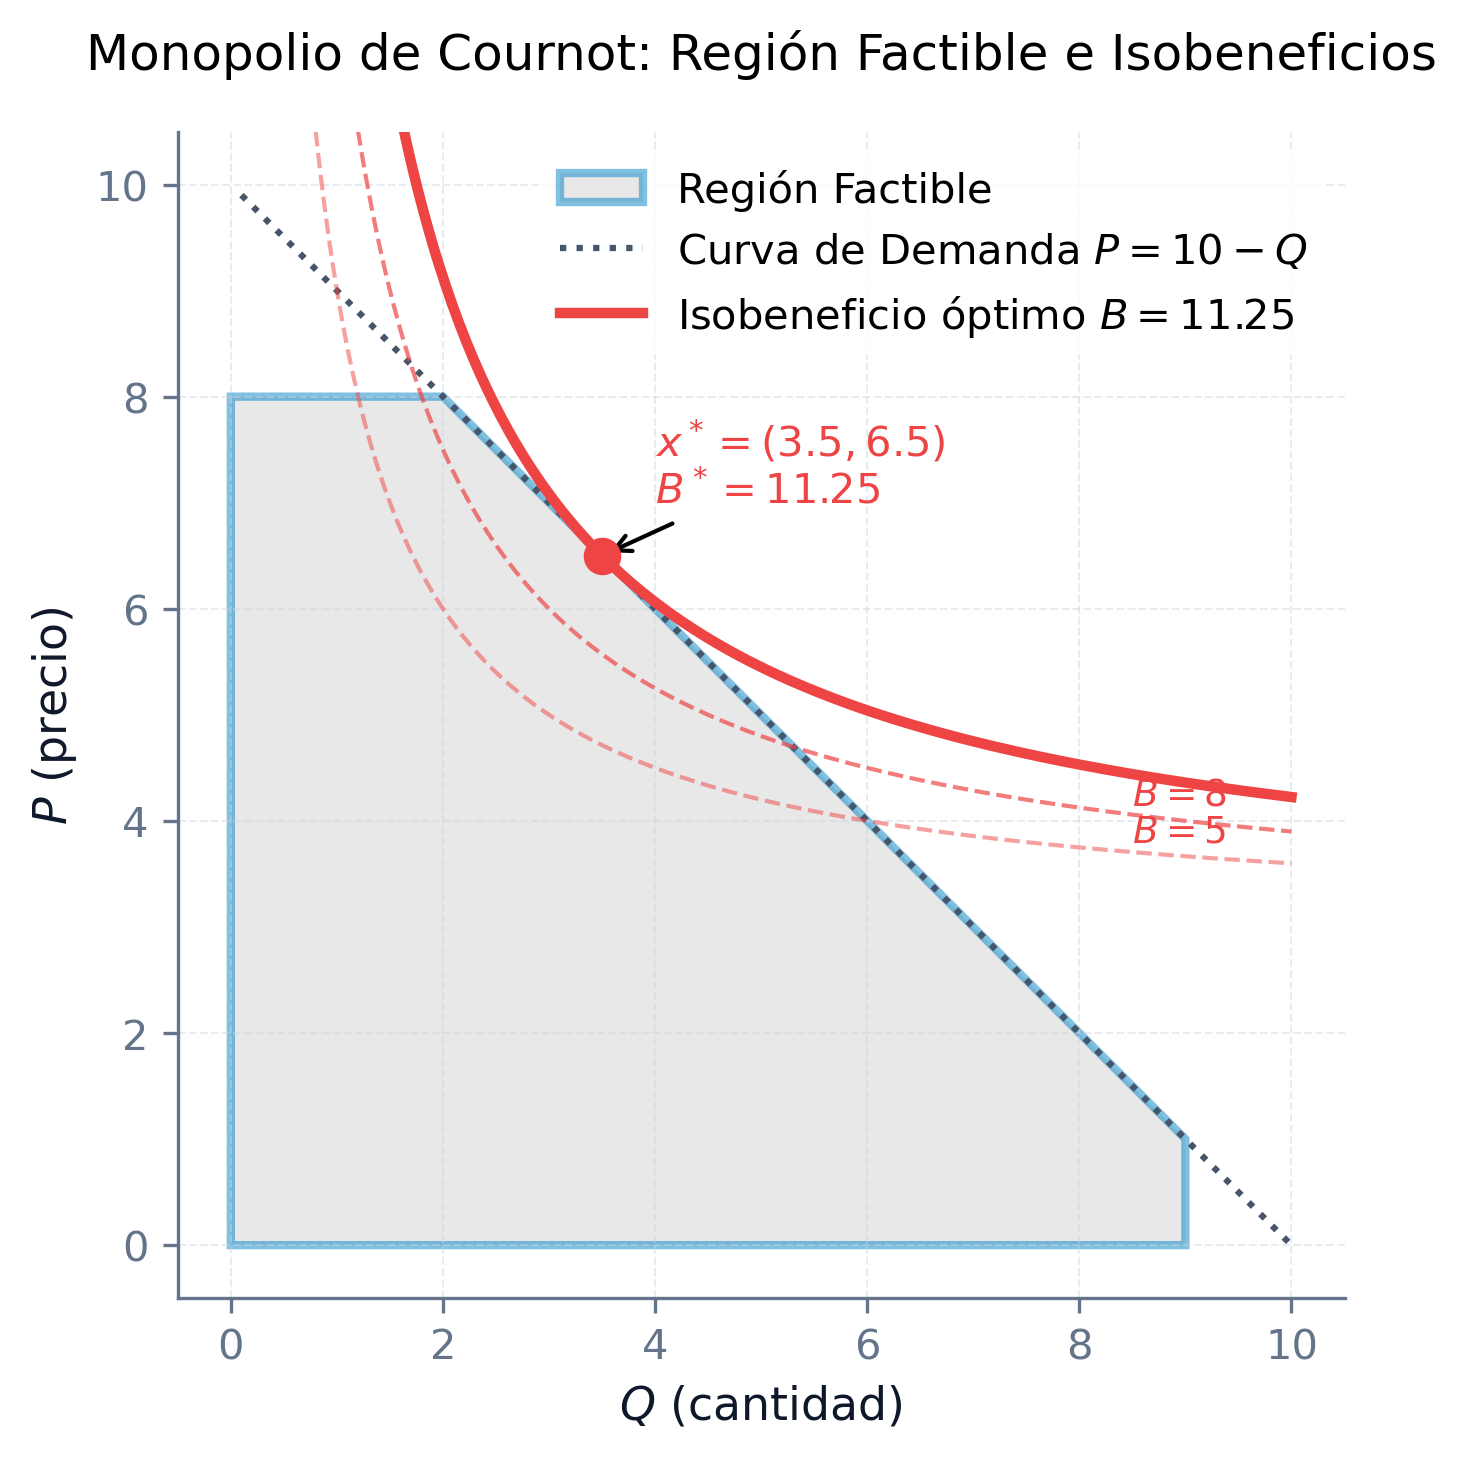
\includegraphics[width=0.5\linewidth,height=\textheight,keepaspectratio]{images/cournot_monopolio.png}

}

\caption{\label{fig-cournot-monopolio}Geometría del Monopolio de
Cournot: el óptimo de tangencia (3.5, 6.5) se sitúa en la frontera y no
coincide con ningún vértice de la región factible polimórfica}

\end{figure}%

Este resultado ilustra la diferencia fundamental con la programación
lineal: la solución óptima de un problema no lineal con restricciones
lineales puede situarse en el interior de una de las caras de la región
factible y no en un vértice (los vértices adyacentes son \((2,8)\) y
\((9,1)\), los cuales arrojan beneficios inferiores, de \(9.0\) y
\(8.0\) u.m. respectivamente).

\subsection{Selección de cartera de valores (Markowitz,
1952)}\label{selecciuxf3n-de-cartera-de-valores-markowitz-1952}

Supongamos que disponemos de un capital \(C\) para invertir entre \(n\)
activos financieros, siguiendo el modelo pionero de selección de
carteras de Markowitz (Markowitz 1952). Denotamos por \(x_i\) la
cantidad monetaria asignada al activo \(i\). Cada activo presenta un
rendimiento medio esperado \(\mu_i\), y la relación de variabilidad
conjunta del mercado se modela a través de la covarianza \(\sigma_{ij}\)
entre los activos \(i\) y \(j\). La varianza de la cartera (medida del
riesgo o volatilidad) viene dada por la forma cuadrática
\(\sum_{i=1}^n \sum_{j=1}^n \sigma_{ij} x_i x_j\).

El inversor busca maximizar el rendimiento esperado de la cartera al
tiempo que minimiza su riesgo, penalizándolo mediante un coeficiente de
aversión al riesgo \(\beta > 0\). El problema se formula como:

\[
\begin{aligned}
\max_{x \in \mathbb{R}^n} \quad & \sum_{i=1}^n \mu_i x_i - \beta \sum_{i=1}^n \sum_{j=1}^n \sigma_{ij} x_i x_j \\
\text{sujeto a} \quad & \sum_{i=1}^n x_i \le C \\
& x_i \ge 0, \quad i = 1, \dots, n
\end{aligned}
\]

Este problema posee una función objetivo cuadrática no lineal y
restricciones lineales, lo que constituye un problema clásico de
\textbf{Programación Cuadrática (QP)}. Su naturaleza estrictamente
convexa (cuando la matriz de covarianzas es semidefinida positiva)
asegura que cualquier óptimo local sea también el óptimo global del
sistema (Boyd y Vandenberghe 2004; Hillier y Lieberman 2010).

\section{Óptimos locales, globales y puntos de
silla}\label{uxf3ptimos-locales-globales-y-puntos-de-silla}

Sea \(f: \mathbb{R}^n \to \mathbb{R}\) una función real definida sobre
un conjunto factible \(\mathcal{X} \subseteq \mathbb{R}^n\). Un punto
\(x^* \in \mathcal{X}\) es un \textbf{mínimo global} si no existe ningún
otro punto factible con un valor inferior de la función objetivo, es
decir, \(f(x) \ge f(x^*)\) para todo \(x \in \mathcal{X}\). Del mismo
modo, \(x^*\) es un \textbf{mínimo global estricto} si se cumple que
\(f(x) > f(x^*)\) para cualquier
\(x \in \mathcal{X} \setminus \{x^*\}\).

Por otro lado, un punto \(x^*\) constituye un \textbf{mínimo local} si
es la mejor solución dentro de un entorno local delimitado por una bola
de radio \(\epsilon > 0\) centrada en él, satisfaciendo
\(f(x) \ge f(x^*)\) para todo \(x \in \mathcal{X}\) tal que
\(\|x - x^*\| \le \epsilon\). Finalmente, \(x^*\) es un \textbf{mínimo
local estricto} si existe un radio \(\epsilon > 0\) tal que
\(f(x) > f(x^*)\) para todo \(x \in \mathcal{X} \setminus \{x^*\}\) con
\(\|x - x^*\| \le \epsilon\).

En optimización no lineal general, debido a la posible presencia de no
convexidades, los algoritmos locales basados en derivadas pueden
converger hacia mínimos locales mediocres en lugar de alcanzar el óptimo
global. Esta es la complejidad fundamental que diferencia al PNL de la
programación lineal (como se ilustra en la
Figura~\ref{fig-tipos-optimos}).

\begin{figure}

\centering{

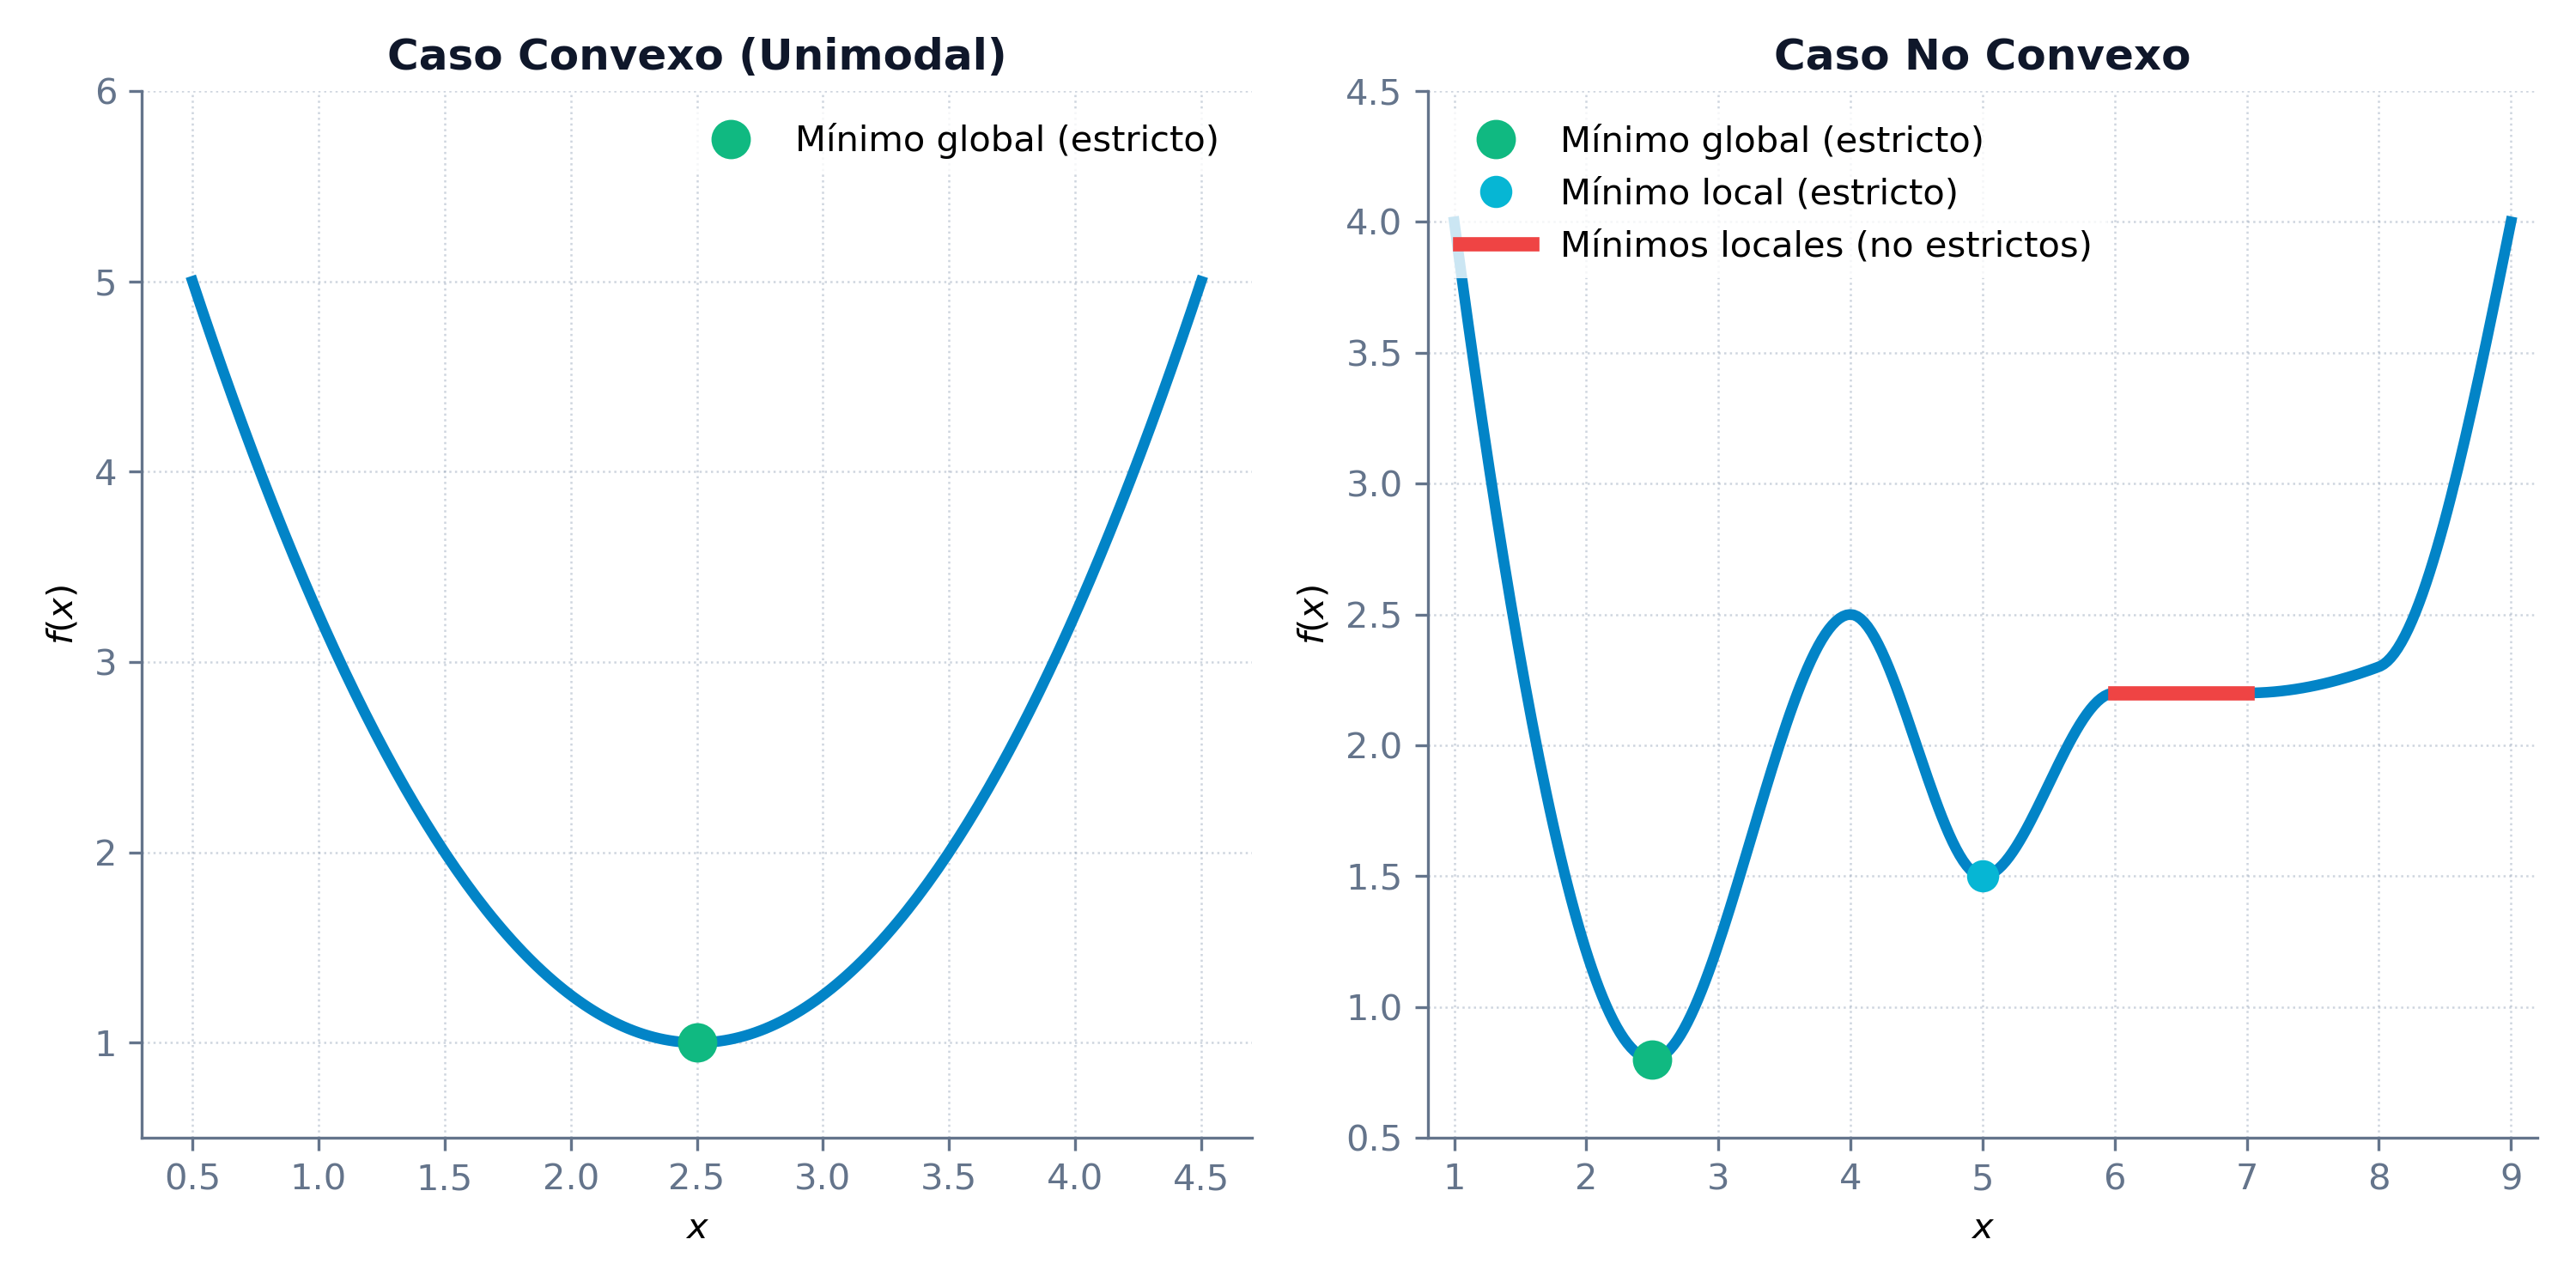
\includegraphics[width=0.95\linewidth,height=\textheight,keepaspectratio]{images/tipos_optimos.png}

}

\caption{\label{fig-tipos-optimos}Ilustración de los distintos tipos de
óptimos locales y globales (estrictos y no estrictos) sobre funciones
convexas y no convexas}

\end{figure}%

\section{Herramientas de análisis
diferencial}\label{herramientas-de-anuxe1lisis-diferencial}

Para caracterizar y clasificar los puntos óptimos locales en múltiples
dimensiones, recurrimos al cálculo diferencial. Consideremos una función
\(f: \mathbb{R}^n \to \mathbb{R}\) diferenciable de clase
\(\mathcal{C}^2\) (con segundas derivadas continuas).

El \textbf{vector gradiente} representa la dirección de máxima pendiente
de subida local de la función y se define como el vector columna de
derivadas parciales de primer orden:
\[ \nabla f(x) = \begin{pmatrix} \frac{\partial f(x)}{\partial x_1} \\ \frac{\partial f(x)}{\partial x_2} \\ \vdots \\ \frac{\partial f(x)}{\partial x_n} \end{pmatrix} \]
Por su parte, la \textbf{matriz hessiana} modela la curvatura local de
la función (análoga a la segunda derivada en una dimensión) y se define
como la matriz simétrica de segundas derivadas parciales:
\[ [\nabla^2 f(x)]_{ij} = \frac{\partial^2 f(x)}{\partial x_i \partial x_j} \]

\subsection{Desarrollo de Taylor
multivariante}\label{desarrollo-de-taylor-multivariante}

El comportamiento local de una función no lineal alrededor de un punto
de referencia \(\bar{x}\) se aproxima mediante su desarrollo cuadrático
de Taylor:

\[ f(x) = f(\bar{x}) + \nabla f(\bar{x})^T (x - \bar{x}) + \frac{1}{2} (x - \bar{x})^T \nabla^2 f(\bar{x}) (x - \bar{x}) + o(\|x - \bar{x}\|^2) \]

Si la función \(f(x)\) es cuadrática, esta aproximación de segundo orden
es exacta para todo \(x \in \mathbb{R}^n\).

\subsection{Caracterización de curvatura y clasificación de
matrices}\label{caracterizaciuxf3n-de-curvatura-y-clasificaciuxf3n-de-matrices}

La curvatura local de la función está determinada por el carácter de su
matriz hessiana \(\nabla^2 f(x)\), el cual se clasifica analizando la
forma cuadrática: \[ z^T \nabla^2 f(x) z \]

\begin{itemize}
\tightlist
\item
  \textbf{Definida positiva (\(\nabla^2 f(x) \succ 0\))}: Si
  \(z^T \nabla^2 f(x) z > 0\) para todo vector no nulo
  \(z \in \mathbb{R}^n\). Todos sus autovalores son estrictamente
  positivos y todos sus menores principales son mayores que cero. La
  función se curva hacia arriba en forma de cuenco, lo que garantiza que
  un punto crítico sea un mínimo local estricto.
\item
  \textbf{Semidefinida positiva (\(\nabla^2 f(x) \succeq 0\))}: Si
  \(z^T \nabla^2 f(x) z \ge 0\) para todo vector \(z \in \mathbb{R}^n\).
  Todos sus autovalores son no negativos y todos sus menores principales
  son no negativos.
\item
  \textbf{Definida negativa (\(\nabla^2 f(x) \prec 0\))}: Si
  \(z^T \nabla^2 f(x) z < 0\) para todo vector no nulo
  \(z \in \mathbb{R}^n\). Sus menores principales alternan de signo
  comenzando por negativo (\(M_1 < 0, M_2 > 0, M_3 < 0, \dots\)) y todos
  sus autovalores son estrictamente negativos. La función se curva hacia
  abajo en forma de cúpula.
\item
  \textbf{Semidefinida negativa (\(\nabla^2 f(x) \preceq 0\))}: Si
  \(z^T \nabla^2 f(x) z \le 0\) para todo vector \(z\). Todos sus
  autovalores son no positivos y todos sus menores principales alternan
  de signo de forma no estricta o son nulos.
\item
  \textbf{Indefinida}: Si existen autovalores estrictamente positivos y
  negativos. El punto crítico resultante constituye un \textbf{punto de
  silla} (con direcciones de subida y direcciones de bajada).
\end{itemize}

\begin{tcolorbox}[enhanced jigsaw, toprule=.15mm, opacitybacktitle=0.6, coltitle=black, colbacktitle=quarto-callout-tip-color!10!white, title=\textcolor{quarto-callout-tip-color}{\faLightbulb}\hspace{0.5em}{Ejemplos: Clasificación de matrices}, arc=.35mm, rightrule=.15mm, toptitle=1mm, breakable, bottomtitle=1mm, titlerule=0mm, colback=white, opacityback=0, leftrule=.75mm, colframe=quarto-callout-tip-color-frame, left=2mm, bottomrule=.15mm]

\begin{enumerate}
\def\labelenumi{\arabic{enumi}.}
\item
  \textbf{Matriz Definida Positiva}: Sea la matriz:
  \[ A_1 = \begin{pmatrix} 2 & 1 \\ 1 & 2 \end{pmatrix} \] Sus menores
  principales son:
  \[ M_1 = |2| = 2 > 0 \qquad \text{y} \qquad M_2 = \det(A_1) = 4 - 1 = 3 > 0 \]
  Al ser ambos menores principales estrictamente positivos, se tiene que
  \(A_1 \succ 0\).

  Resolviendo el polinomio característico:
  \[ \det(A_1 - \lambda I) = (2-\lambda)^2 - 1 = 0 \implies \lambda^2 - 4\lambda + 3 = 0 \]
  obtenemos los autovalores \(\lambda_1 = 3\) y \(\lambda_2 = 1\), los
  cuales confirman que es definida positiva.
\item
  \textbf{Matriz Indefinida}: Sea la matriz:
  \[ A_2 = \begin{pmatrix} 1 & 2 \\ 2 & 1 \end{pmatrix} \] Sus menores
  principales son:
  \[ M_1 = |1| = 1 > 0 \qquad \text{y} \qquad M_2 = \det(A_2) = 1 - 4 = -3 < 0 \]
  Dado que el determinante de segundo orden es negativo, la matriz es
  indefinida.

  Resolviendo el polinomio característico:
  \[ \det(A_2 - \lambda I) = (1-\lambda)^2 - 4 = 0 \implies \lambda^2 - 2\lambda - 3 = 0 \]
  hallamos los autovalores \(\lambda_1 = 3\) (positivo) y
  \(\lambda_2 = -1\) (negativo), lo que ratifica el carácter indefinido.
\item
  \textbf{Matriz Semidefinida Positiva}: Sea la matriz:
  \[ A_3 = \begin{pmatrix} 2 & -3 & -1 \\ -3 & 12 & 6 \\ -1 & 6 & 3.2 \end{pmatrix} \]
  Sus menores principales de primer y segundo orden son:
  \[ M_1 = |2| = 2 > 0 \qquad \text{y} \qquad M_2 = 24 - 9 = 15 > 0 \] y
  su determinante (menor principal de tercer orden):
  \[ M_3 = \det(A_3) = 2(38.4 - 36) + 3(-9.6 + 6) - 1(-18 + 12) = 4.8 - 10.8 + 6 = 0 \]
  Al ser todos los menores principales no negativos y el determinante
  nulo, la matriz es semidefinida positiva y singular. Sus autovalores
  son \(\lambda_1 \approx 15.75\), \(\lambda_2 \approx 1.45\), y
  \(\lambda_3 = 0\), confirmando la semidefinición (\(A_3 \succeq 0\)).
\end{enumerate}

\end{tcolorbox}

\subsection{Condiciones de optimalidad y puntos
estacionarios}\label{condiciones-de-optimalidad-y-puntos-estacionarios}

Las condiciones diferenciales para determinar extremos locales se
enuncian en el siguiente teorema.

\begin{tcolorbox}[enhanced jigsaw, toprule=.15mm, opacitybacktitle=0.6, coltitle=black, colbacktitle=quarto-callout-important-color!10!white, title=\textcolor{quarto-callout-important-color}{\faExclamation}\hspace{0.5em}{Teorema: Condiciones de optimalidad de segundo orden}, arc=.35mm, rightrule=.15mm, toptitle=1mm, breakable, bottomtitle=1mm, titlerule=0mm, colback=white, opacityback=0, leftrule=.75mm, colframe=quarto-callout-important-color-frame, left=2mm, bottomrule=.15mm]

Sea \(f: \mathbb{R}^n \to \mathbb{R}\) una función diferenciable de
clase \(\mathcal{C}^2\):

\begin{enumerate}
\def\labelenumi{\arabic{enumi}.}
\tightlist
\item
  \textbf{Condición Necesaria de Primer Orden (FONC)}: Si \(x^*\) es un
  mínimo local, entonces el gradiente de la función se anula en dicho
  punto: \[ \nabla f(x^*) = 0 \] Cualquier punto que verifique esta
  condición se denomina \textbf{punto estacionario} o punto crítico.
\item
  \textbf{Condición Necesaria de Segundo Orden (SONC)}: Si \(x^*\) es un
  mínimo local, entonces además de cumplirse la FONC, la matriz hessiana
  en dicho punto es semidefinida positiva:
  \[ \nabla^2 f(x^*) \succeq 0 \]
\item
  \textbf{Condición Suficiente de Segundo Orden (SOSC)}: Si un punto
  \(x^*\) satisface simultáneamente que:
  \[ \nabla f(x^*) = 0 \qquad \text{y} \qquad \nabla^2 f(x^*) \succ 0 \]
  Entonces \(x^*\) es un \textbf{mínimo local estricto} de la función.
\end{enumerate}

\end{tcolorbox}

\begin{tcolorbox}[enhanced jigsaw, toprule=.15mm, opacitybacktitle=0.6, coltitle=black, colbacktitle=quarto-callout-warning-color!10!white, title=\textcolor{quarto-callout-warning-color}{\faExclamationTriangle}\hspace{0.5em}{Importancia de la definición positiva en SOSC}, arc=.35mm, rightrule=.15mm, toptitle=1mm, breakable, bottomtitle=1mm, titlerule=0mm, colback=white, opacityback=0, leftrule=.75mm, colframe=quarto-callout-warning-color-frame, left=2mm, bottomrule=.15mm]

Es fundamental notar que en la condición suficiente (SOSC), la matriz
hessiana debe ser \textbf{estrictamente definida positiva}
(\(\nabla^2 f(x^*) \succ 0\)) y no simplemente semidefinida positiva. Si
la hessiana es semidefinida con algún autovalor nulo (por ejemplo, en la
función \(f(x) = x^4\) en el origen \(x^*=0\), donde \(f'(0)=0\) y
\(f''(0)=0 \succeq 0\)), el análisis de segundo orden es insuficiente
para garantizar analíticamente si el punto es un mínimo, un máximo o un
punto de inflexión.

\end{tcolorbox}

\begin{tcolorbox}[enhanced jigsaw, toprule=.15mm, opacitybacktitle=0.6, coltitle=black, colbacktitle=quarto-callout-tip-color!10!white, title=\textcolor{quarto-callout-tip-color}{\faLightbulb}\hspace{0.5em}{Ejemplos: Clasificación de puntos estacionarios}, arc=.35mm, rightrule=.15mm, toptitle=1mm, breakable, bottomtitle=1mm, titlerule=0mm, colback=white, opacityback=0, leftrule=.75mm, colframe=quarto-callout-tip-color-frame, left=2mm, bottomrule=.15mm]

\begin{enumerate}
\def\labelenumi{\arabic{enumi}.}
\item
  \textbf{Punto de Silla (Hessiana Indefinida)}: Sea la función:
  \[ f(x, y) = \frac{1}{2} x^2 + 2xy + \frac{1}{2} y^2 - y + 9 \] Su
  gradiente se obtiene derivando parcialmente respecto a cada variable:
  \[ \nabla f(x, y) = \begin{pmatrix} x + 2y \\ 2x + y - 1 \end{pmatrix} \]
  Igualando el gradiente a cero, resolvemos el sistema de ecuaciones
  para hallar los puntos críticos:
  \[ \begin{cases} x + 2y = 0 \implies x = -2y \\ 2x + y - 1 = 0 \implies 2(-2y) + y = 1 \implies -3y = 1 \implies y^* = -1/3 \end{cases} \]
  sustituyendo, obtenemos el punto crítico único en
  \((x^*, y^*) = (2/3, -1/3)\).

  La matriz hessiana de la función es:
  \[ \nabla^2 f(x, y) = \begin{pmatrix} 1 & 2 \\ 2 & 1 \end{pmatrix} \]
  Calculamos sus menores principales para clasificarla:
  \[ M_1 = |1| = 1 > 0 \qquad \text{y} \qquad M_2 = \det(\nabla^2 f) = 1 - 4 = -3 < 0 \]
  Al ser el menor principal de segundo orden negativo (\(M_2 < 0\)), la
  matriz hessiana es indefinida. Por tanto, el punto crítico
  \((2/3, -1/3)\) constituye un \textbf{punto de silla}.

  \begin{figure}[H]

  \centering{

  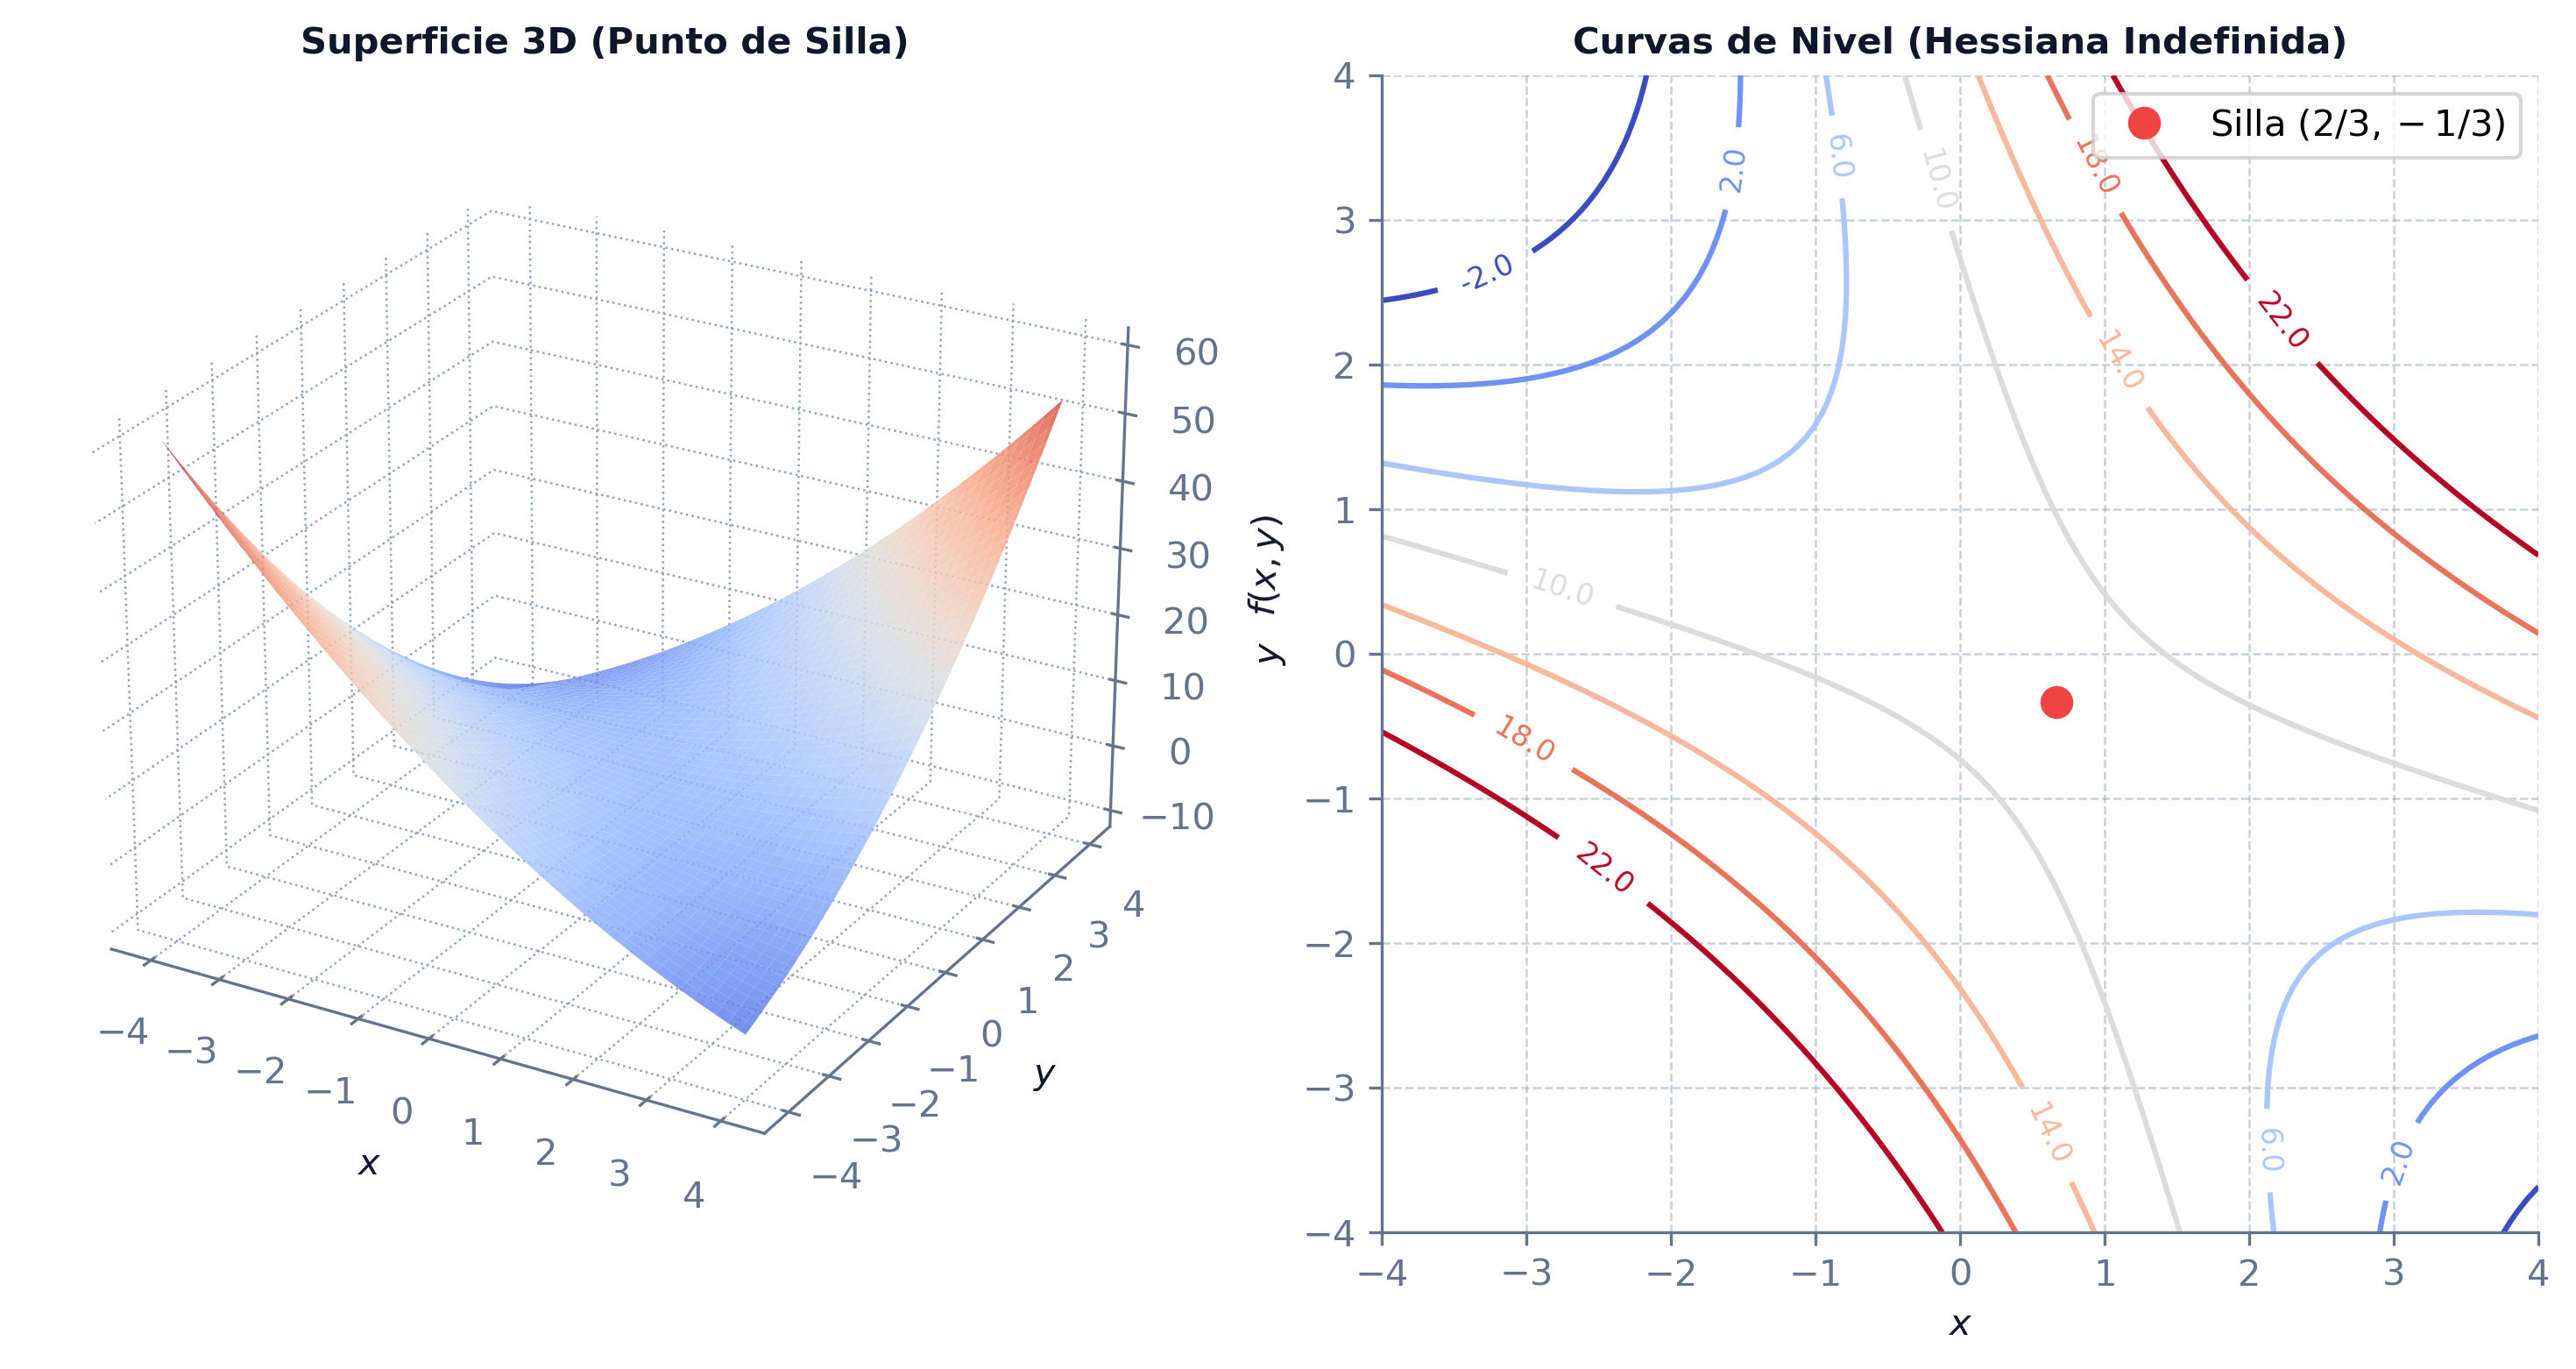
\includegraphics[width=0.95\linewidth,height=\textheight,keepaspectratio]{images/punto_silla_3d.png}

  }

  \caption{\label{fig-superficies-3d-silla}Representación 3D y curvas de
  nivel de un punto de silla (Hessiana indefinida)}

  \end{figure}%
\item
  \textbf{Mínimo Local Estricto Circular (Hessiana Definida Positiva)}:
  Sea la función que mide el cuadrado de la distancia al punto
  \((2, 1)\): \[ f(x, y) = (x-2)^2 + (y-1)^2 \] Su gradiente es:
  \[ \nabla f(x, y) = \begin{pmatrix} 2(x-2) \\ 2(y-1) \end{pmatrix} \]
  Igualando a cero, el gradiente se anula únicamente en el punto crítico
  \((x^*, y^*) = (2, 1)\).

  La matriz hessiana es constante y diagonal:
  \[ \nabla^2 f(x, y) = \begin{pmatrix} 2 & 0 \\ 0 & 2 \end{pmatrix} \]
  Evaluamos los menores principales:
  \[ M_1 = 2 > 0 \qquad \text{y} \qquad M_2 = 4 > 0 \] Dado que ambos
  menores principales son estrictamente positivos, la matriz hessiana es
  definida positiva (\(\nabla^2 f \succ 0\)). Esto clasifica al punto
  crítico \((2, 1)\) como un \textbf{mínimo local estricto} (cuyas
  curvas de nivel son circunferencias concéntricas).

  \begin{figure}[H]

  \centering{

  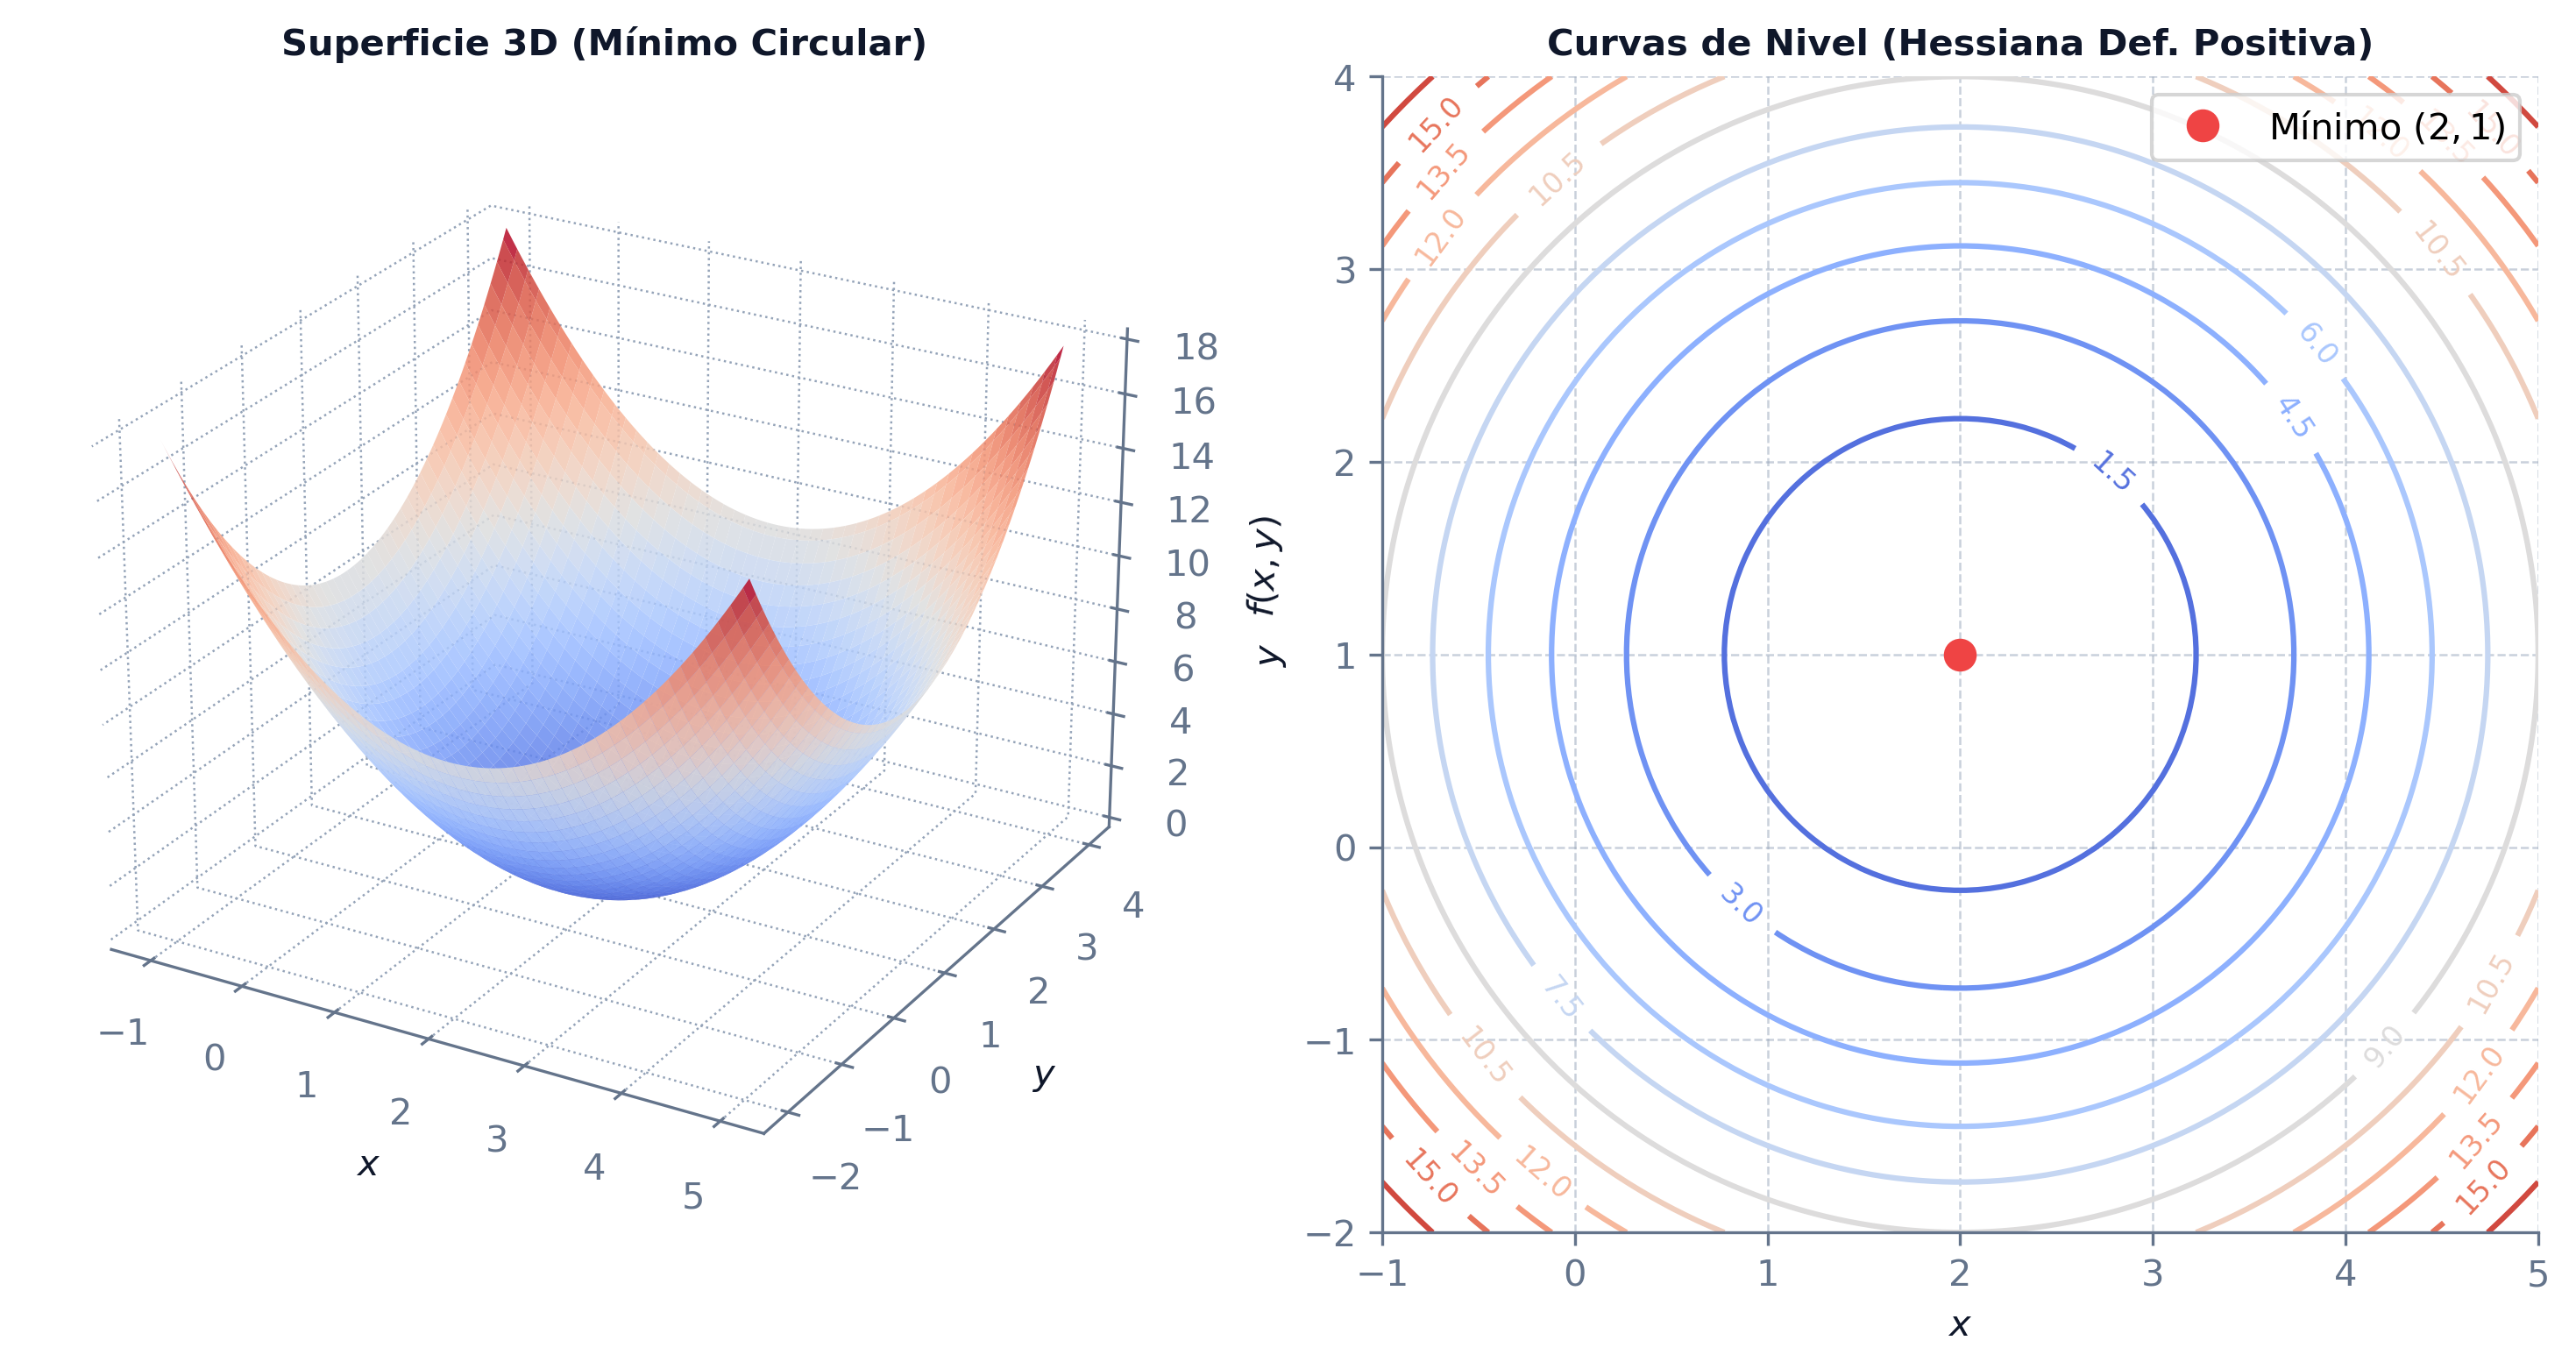
\includegraphics[width=0.95\linewidth,height=\textheight,keepaspectratio]{images/funcion_distancia_3d.png}

  }

  \caption{\label{fig-superficies-3d-circular}Representación 3D y curvas
  de nivel de un mínimo circular (Hessiana definida positiva)}

  \end{figure}%
\item
  \textbf{Mínimo Local Estricto Elíptico (Función Cuadrática Acoplada)}:
  Sea la función con término de acoplamiento cruzado:
  \[ f(x, y) = 8x^2 + 3xy + 7y^2 - 25x + 31y - 29 \] Su gradiente es:
  \[ \nabla f(x, y) = \begin{pmatrix} 16x + 3y - 25 \\ 3x + 14y + 31 \end{pmatrix} \]
  Resolvemos el sistema lineal \(\nabla f(x, y) = 0\):
  \[ \begin{pmatrix} 16 & 3 \\ 3 & 14 \end{pmatrix} \begin{pmatrix} x \\ y \end{pmatrix} = \begin{pmatrix} 25 \\ -31 \end{pmatrix} \implies (x^*, y^*) \approx (2.060, -2.656) \]

  La matriz hessiana es constante:
  \[ \nabla^2 f(x, y) = \begin{pmatrix} 16 & 3 \\ 3 & 14 \end{pmatrix} \]
  Sus menores principales de primer y segundo orden son:
  \[ M_1 = 16 > 0 \qquad \text{y} \qquad M_2 = 16(14) - 3^2 = 224 - 9 = 215 > 0 \]
  Al ser ambos menores principales estrictamente positivos, la matriz es
  definida positiva (\(\nabla^2 f \succ 0\)). Esto confirma que el punto
  crítico \((2.060, -2.656)\) es un \textbf{mínimo local estricto} (con
  curvas de nivel elípticas inclinadas por efecto del acoplamiento).

  \begin{figure}[H]

  \centering{

  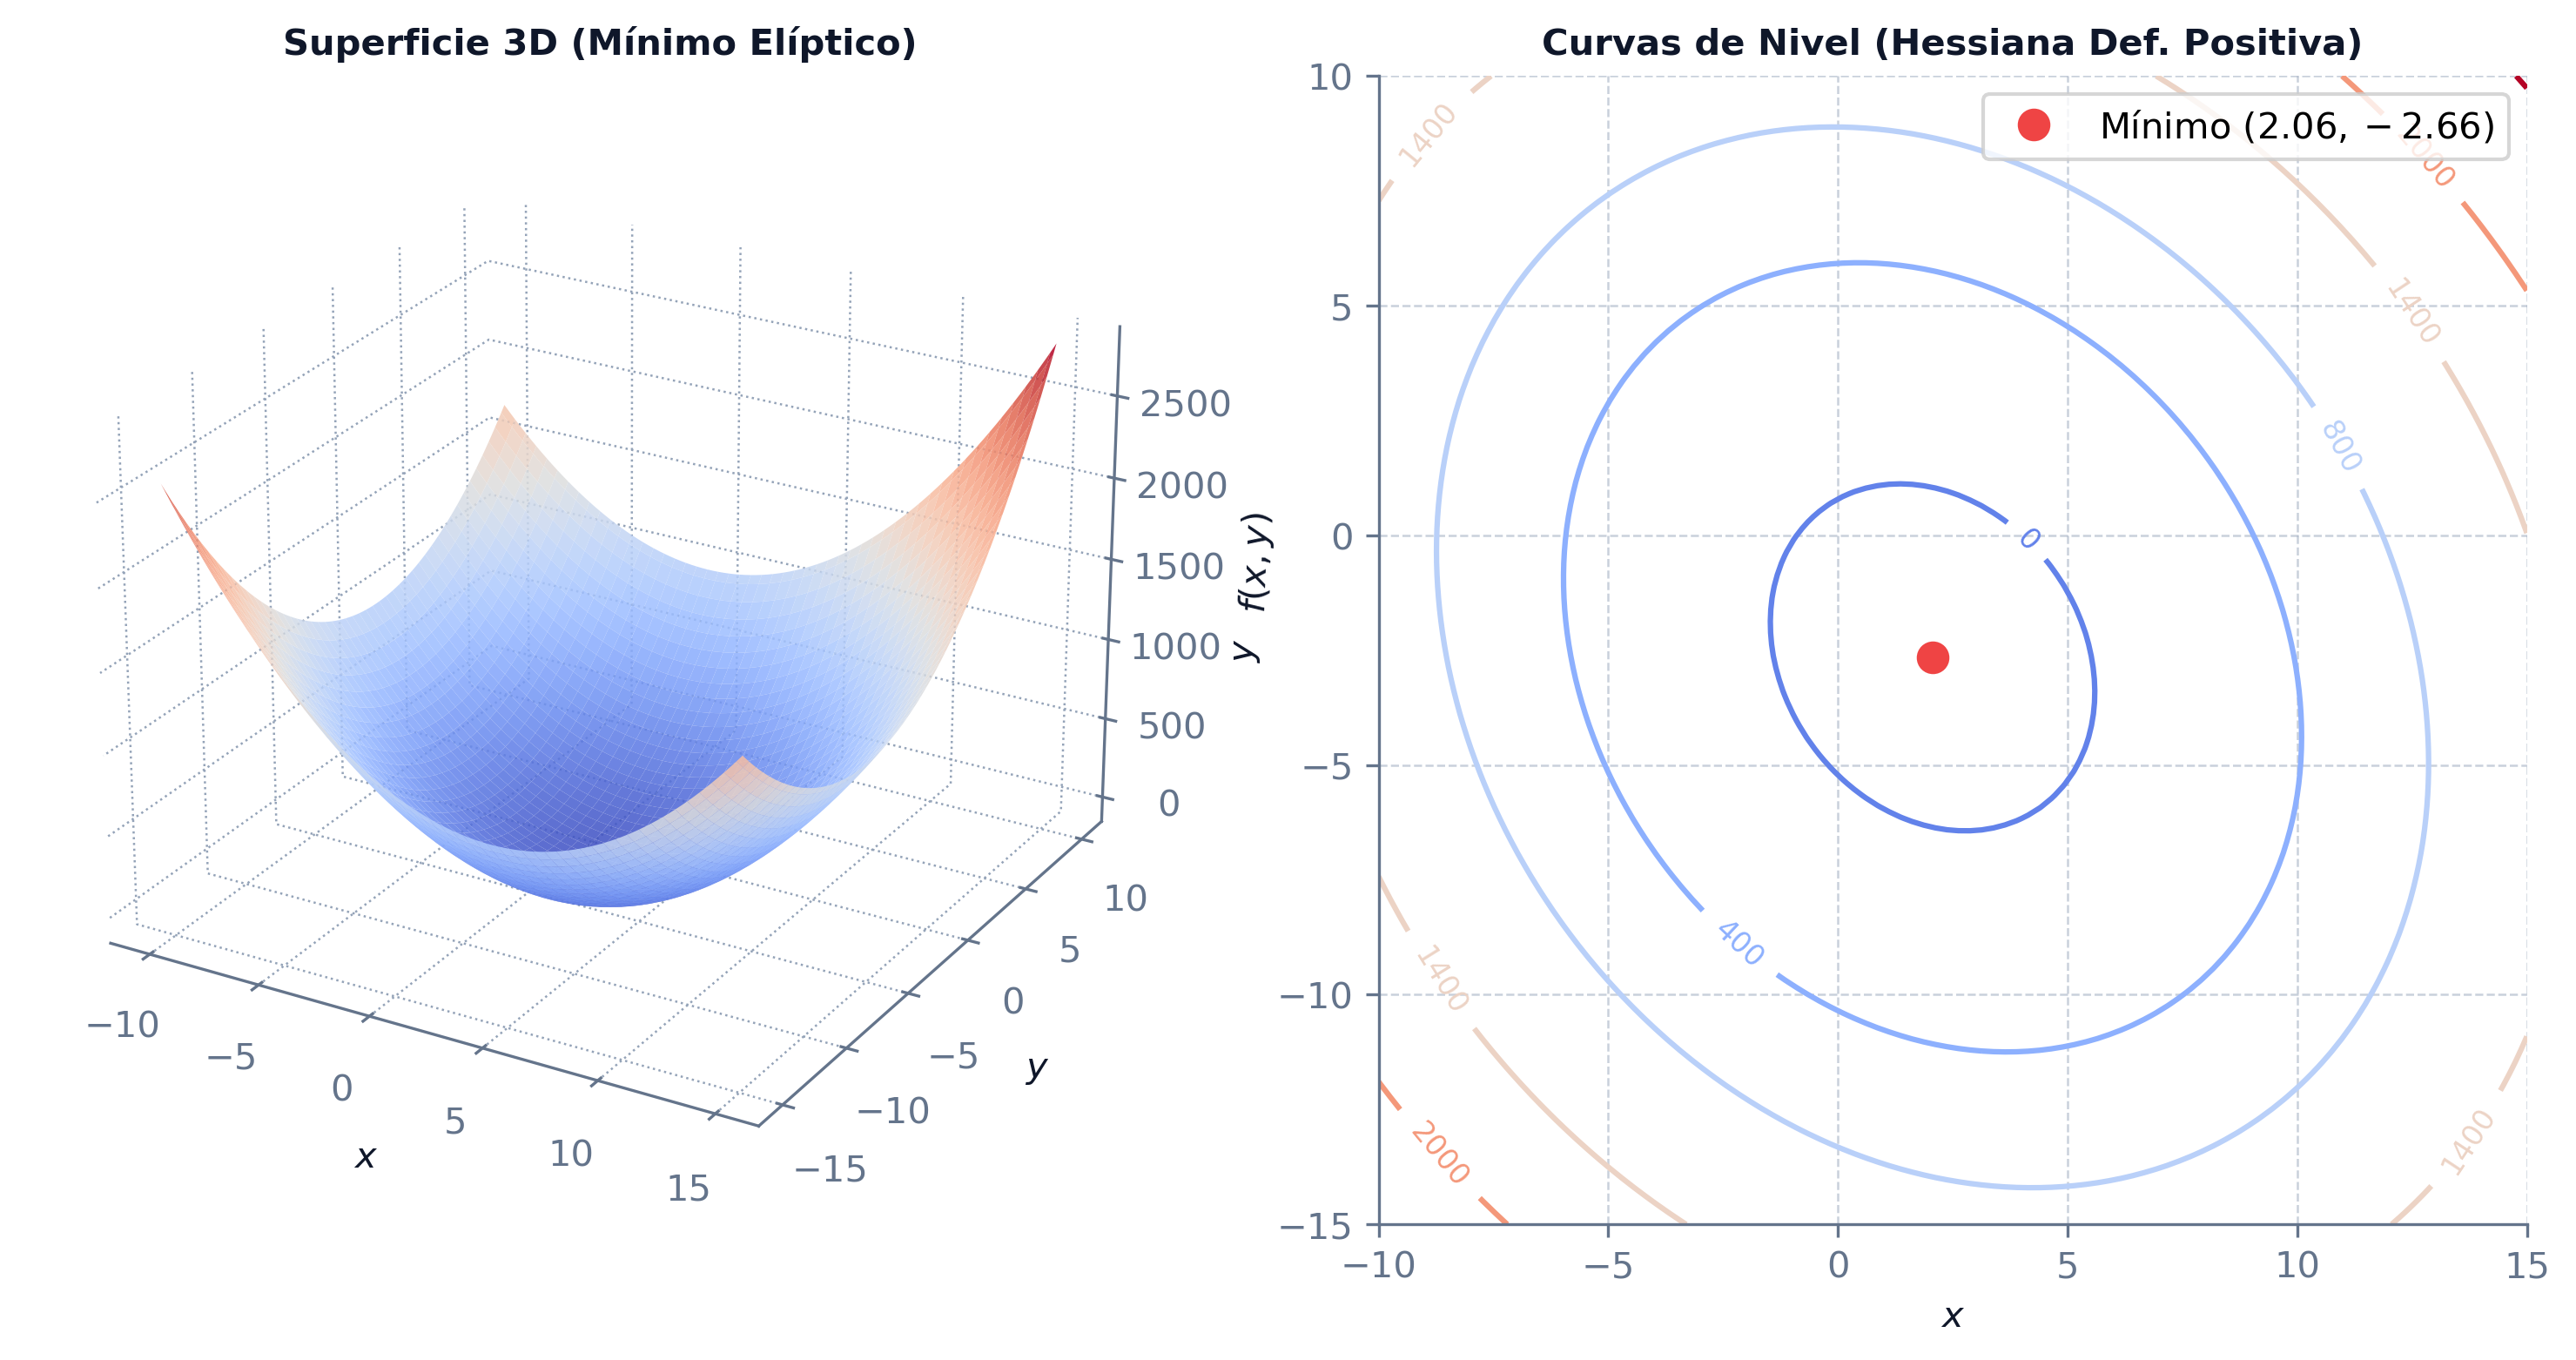
\includegraphics[width=0.95\linewidth,height=\textheight,keepaspectratio]{images/funcion_cuadratica_3d.png}

  }

  \caption{\label{fig-superficies-3d-eliptica}Representación 3D y curvas
  de nivel de un mínimo elíptico (Hessiana definida positiva)}

  \end{figure}%
\end{enumerate}

\end{tcolorbox}

\section{Métodos de búsqueda
unidimensional}\label{muxe9todos-de-buxfasqueda-unidimensional}

Los métodos de búsqueda unidimensional buscan minimizar una función real
de una variable \(f: \mathbb{R} \to \mathbb{R}\) en un intervalo acotado
\([a, b]\). Son fundamentales porque resolver problemas
multidimensionales complejos suele requerir resolver una sucesión de
problemas unidimensionales a lo largo de direcciones de descenso:
\(\min_{\alpha > 0} f(x_k + \alpha d_k)\).

A modo de ilustración de las trazas numéricas de los algoritmos 1D,
utilizaremos como caso de prueba la minimización en el intervalo
\([1, 4]\) de la función de cuarto grado:
\[ f(x) = \frac{1}{4}x^4 - \frac{13}{3}x^3 + 27x^2 - 72x + 1 \] cuyo
gráfico y mínimo global en \(x^* = 3.0\) se muestran en la
Figura~\ref{fig-opt-1d-ejemplo}.

\begin{figure}

\centering{

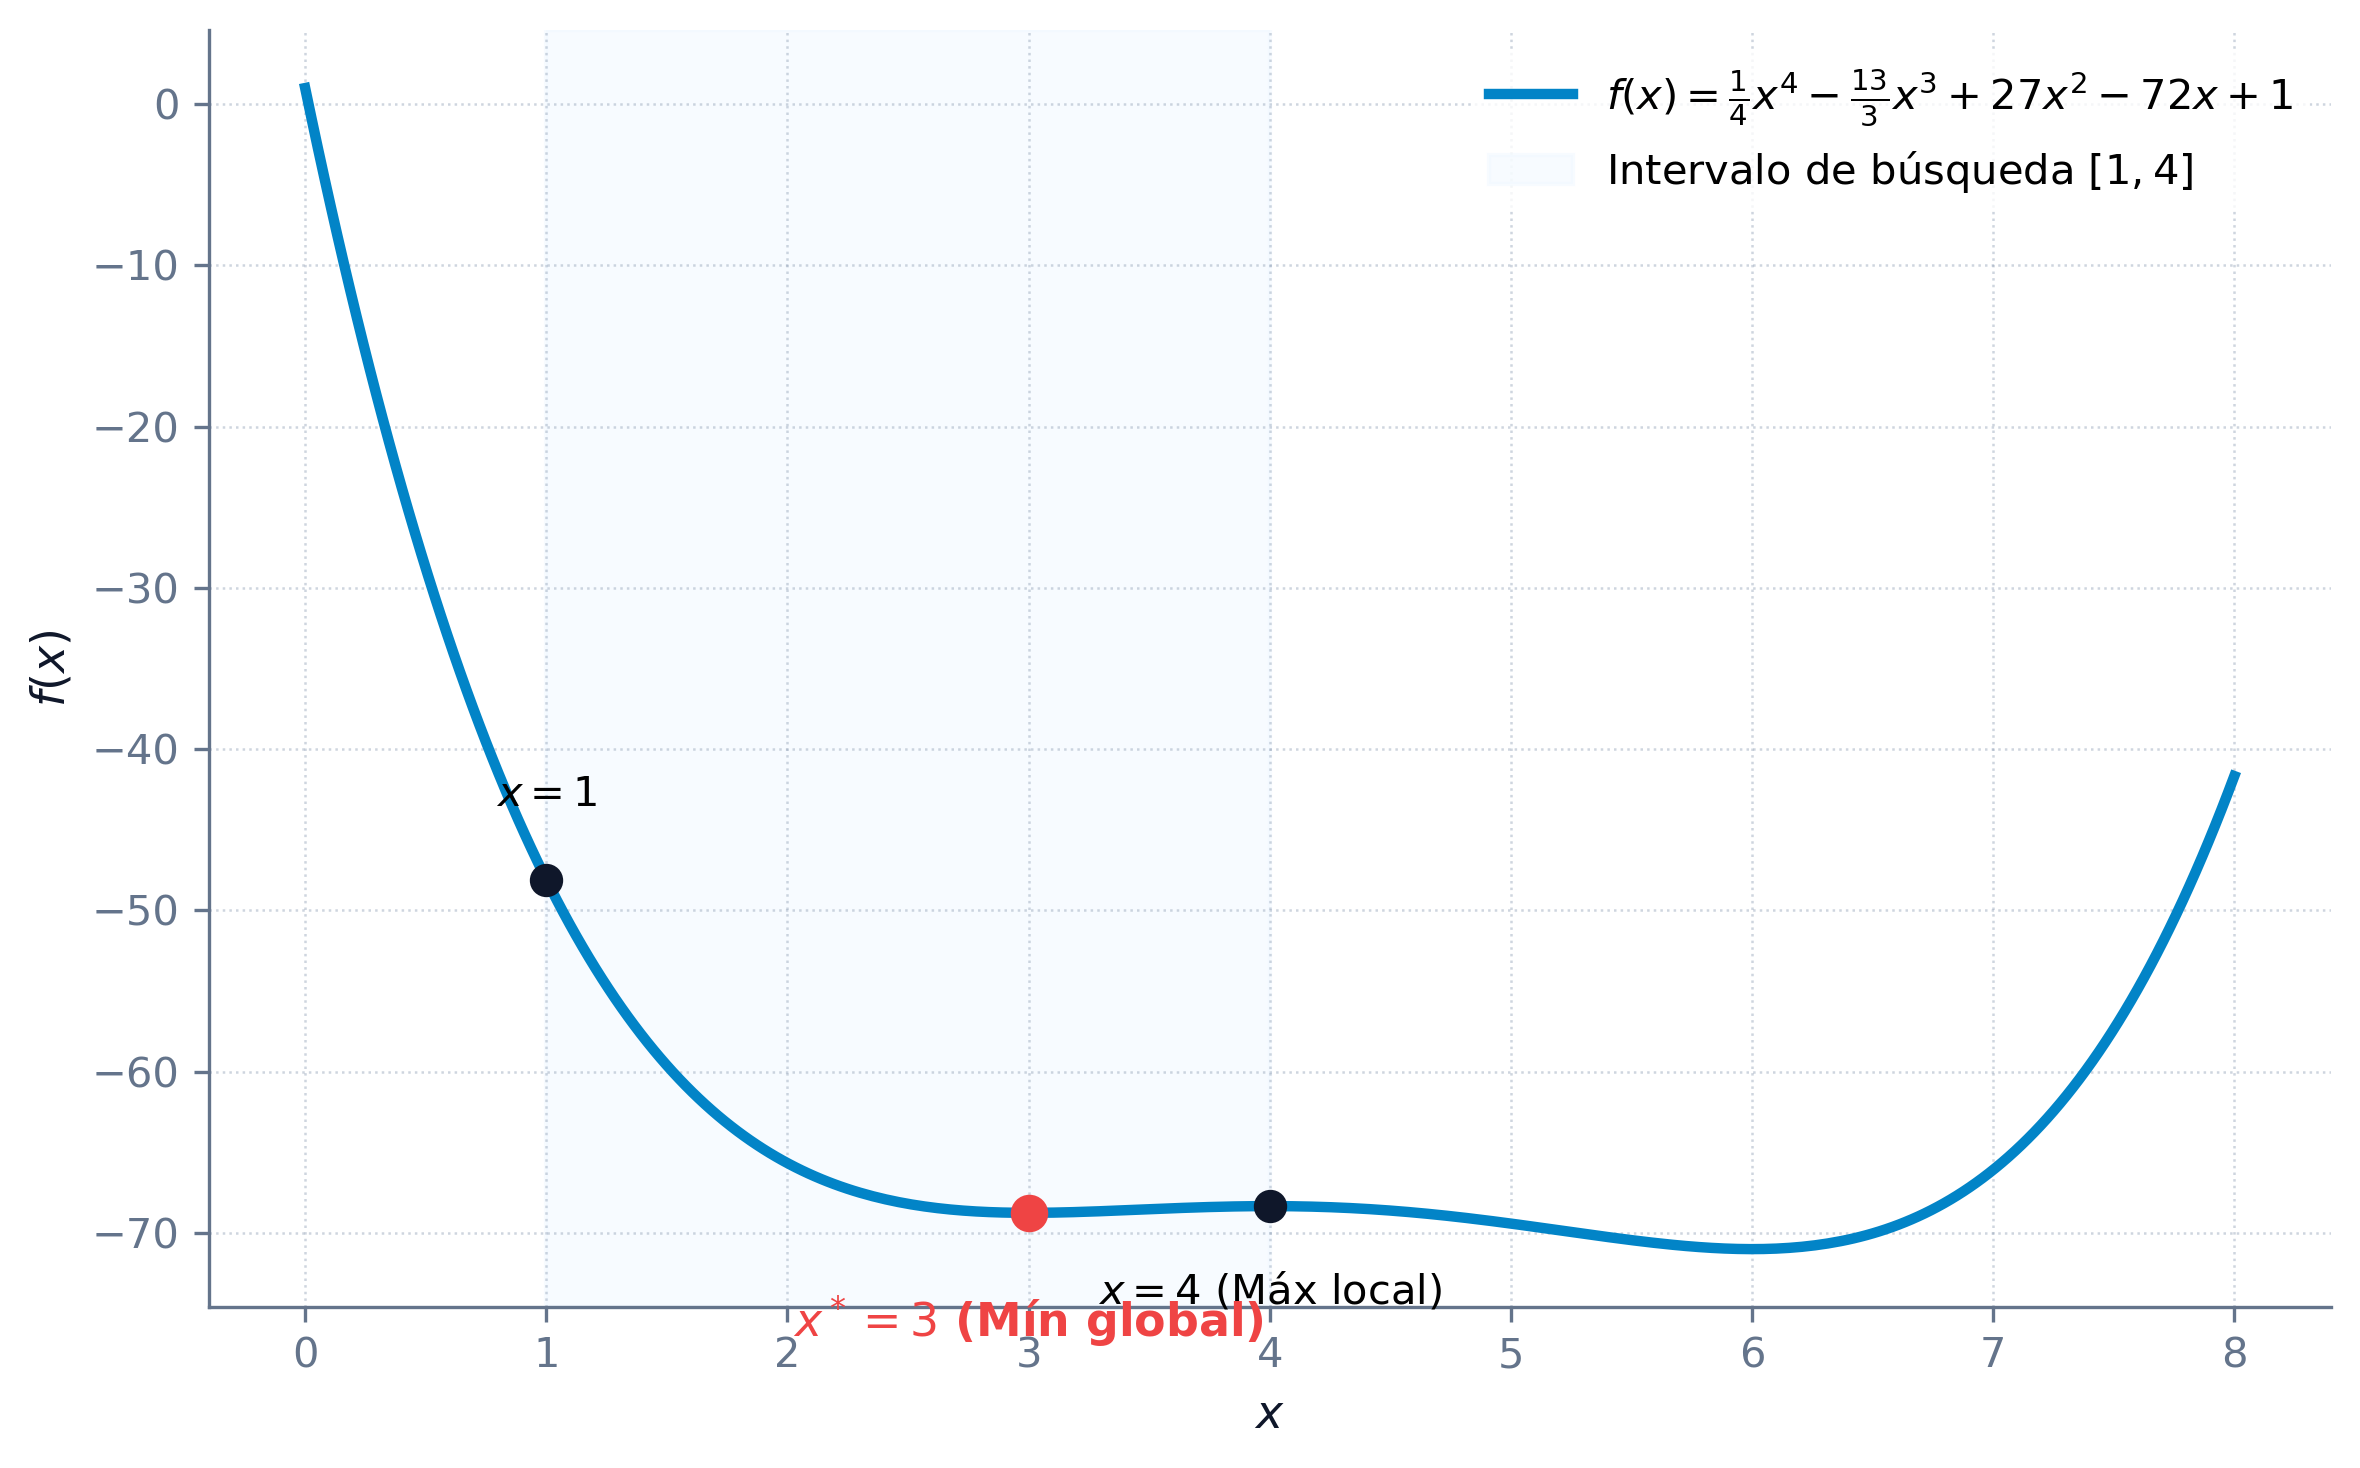
\includegraphics[width=0.7\linewidth,height=\textheight,keepaspectratio]{images/opt_1d_ejemplo.png}

}

\caption{\label{fig-opt-1d-ejemplo}Caso de prueba para métodos de
búsqueda 1D: función de cuarto grado y su mínimo global}

\end{figure}%

\subsection{Métodos sin derivadas}\label{muxe9todos-sin-derivadas}

Estos métodos solo requieren evaluar el valor de la función objetivo.
Exigen que la función sea \textbf{unimodal} en el intervalo \([a, b]\),
es decir, que posea un único mínimo local en dicho intervalo,
decreciendo de forma monótona a la izquierda del mínimo y creciendo a su
derecha.

La \textbf{Búsqueda Uniforme (Rejilla)} consiste en dividir el intervalo
inicial \([a, b]\) en \(n\) subintervalos de igual anchura mediante una
rejilla equidistante de puntos.

Formalmente, los puntos se definen como:
\[x_k = a + k \cdot \frac{b-a}{n}, \quad k = 0, 1, \dots, n\] Evaluamos
la función en todos los puntos de la rejilla para identificar el punto
mínimo: \[k^* = \arg\min_{k \in \{0, \dots, n\}} f(x_k)\] y reducimos el
intervalo de incertidumbre al subintervalo adyacente que rodea al óptimo
muestreado: \[[a', b'] = [x_{k^*-1}, x_{k^*+1}]\] Aunque es un método
muy robusto, resulta poco eficiente debido a que no aprovecha la
información de las evaluaciones previas (ver la
Figura~\ref{fig-busqueda-uniforme-concepto}).

\begin{figure}

\centering{

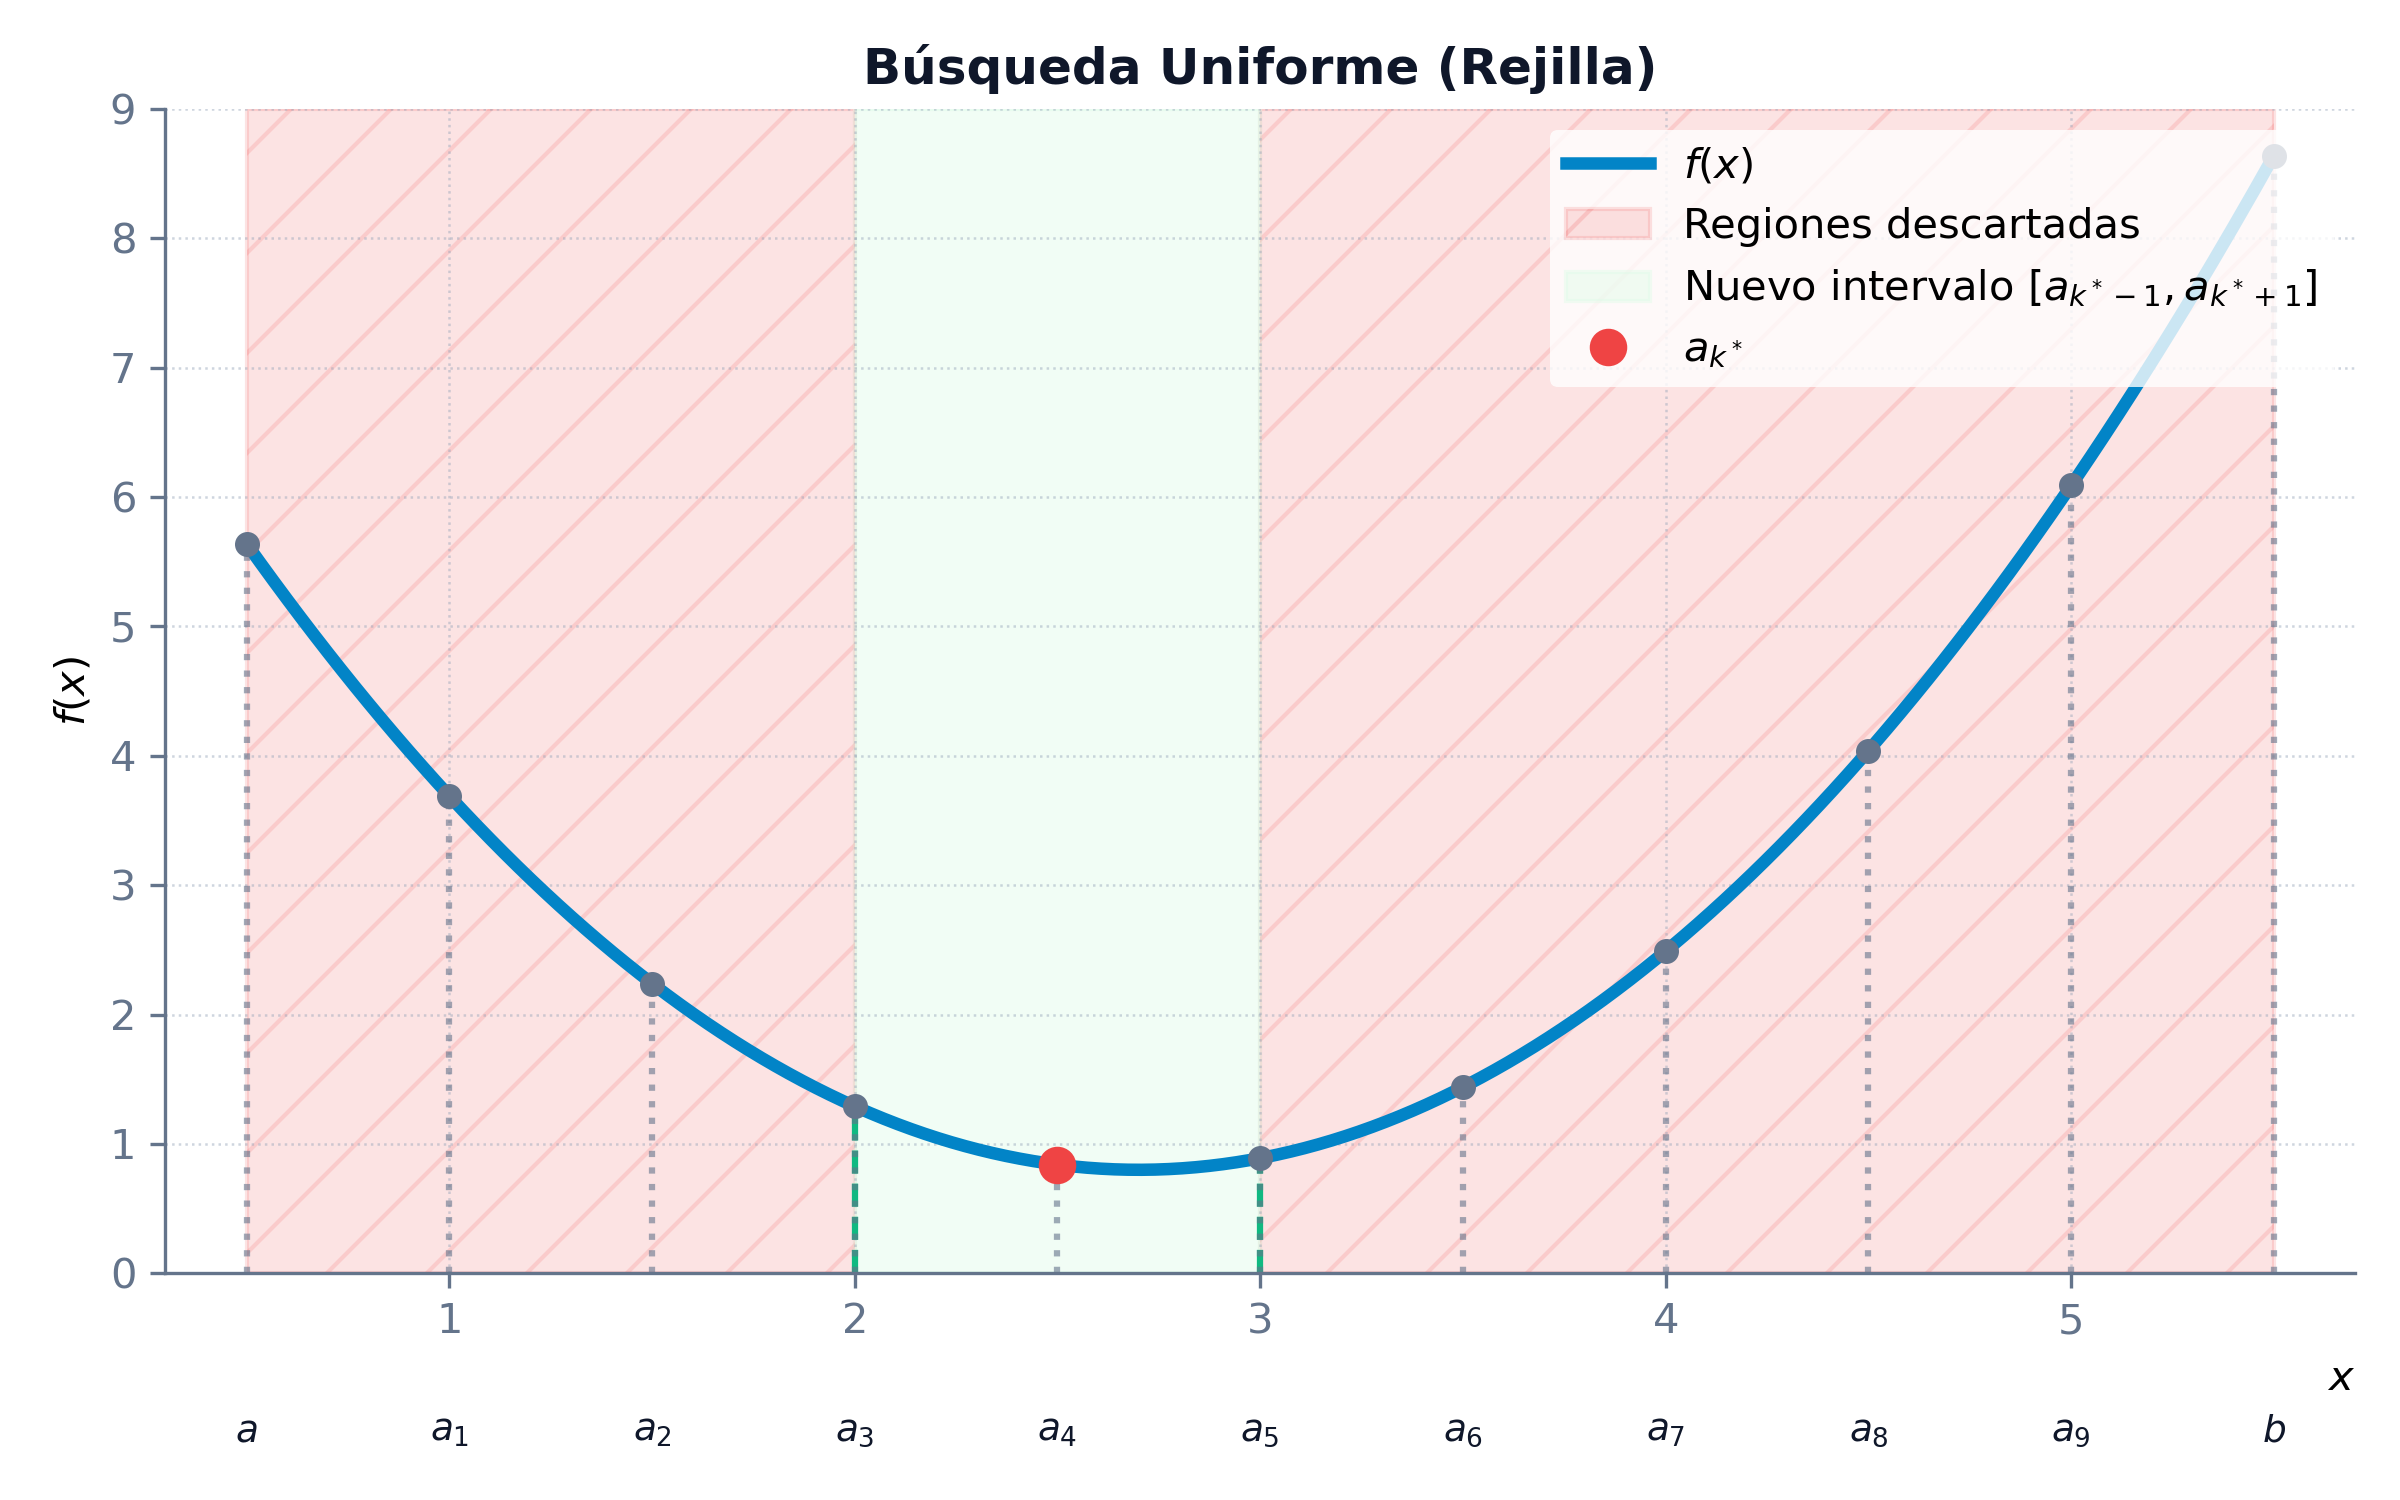
\includegraphics[width=0.7\linewidth,height=\textheight,keepaspectratio]{images/busqueda_uniforme_concepto.png}

}

\caption{\label{fig-busqueda-uniforme-concepto}Concepto de la Búsqueda
Uniforme en rejilla: subdivisión equidistante del intervalo y reducción
basada en el punto mínimo de la muestra}

\end{figure}%

La \textbf{Búsqueda Dicotómica} evalúa la función en el entorno del
punto medio del intervalo actual. Bajo la hipótesis de unimodalidad, si
únicamente evaluásemos la función en el punto medio exacto \(c\), no
tendríamos suficiente información para comparar y deducir si el mínimo
está a la izquierda o a la derecha (ver
Figura~\ref{fig-busqueda-dicotomica-insuficiente}).

\begin{figure}

\centering{

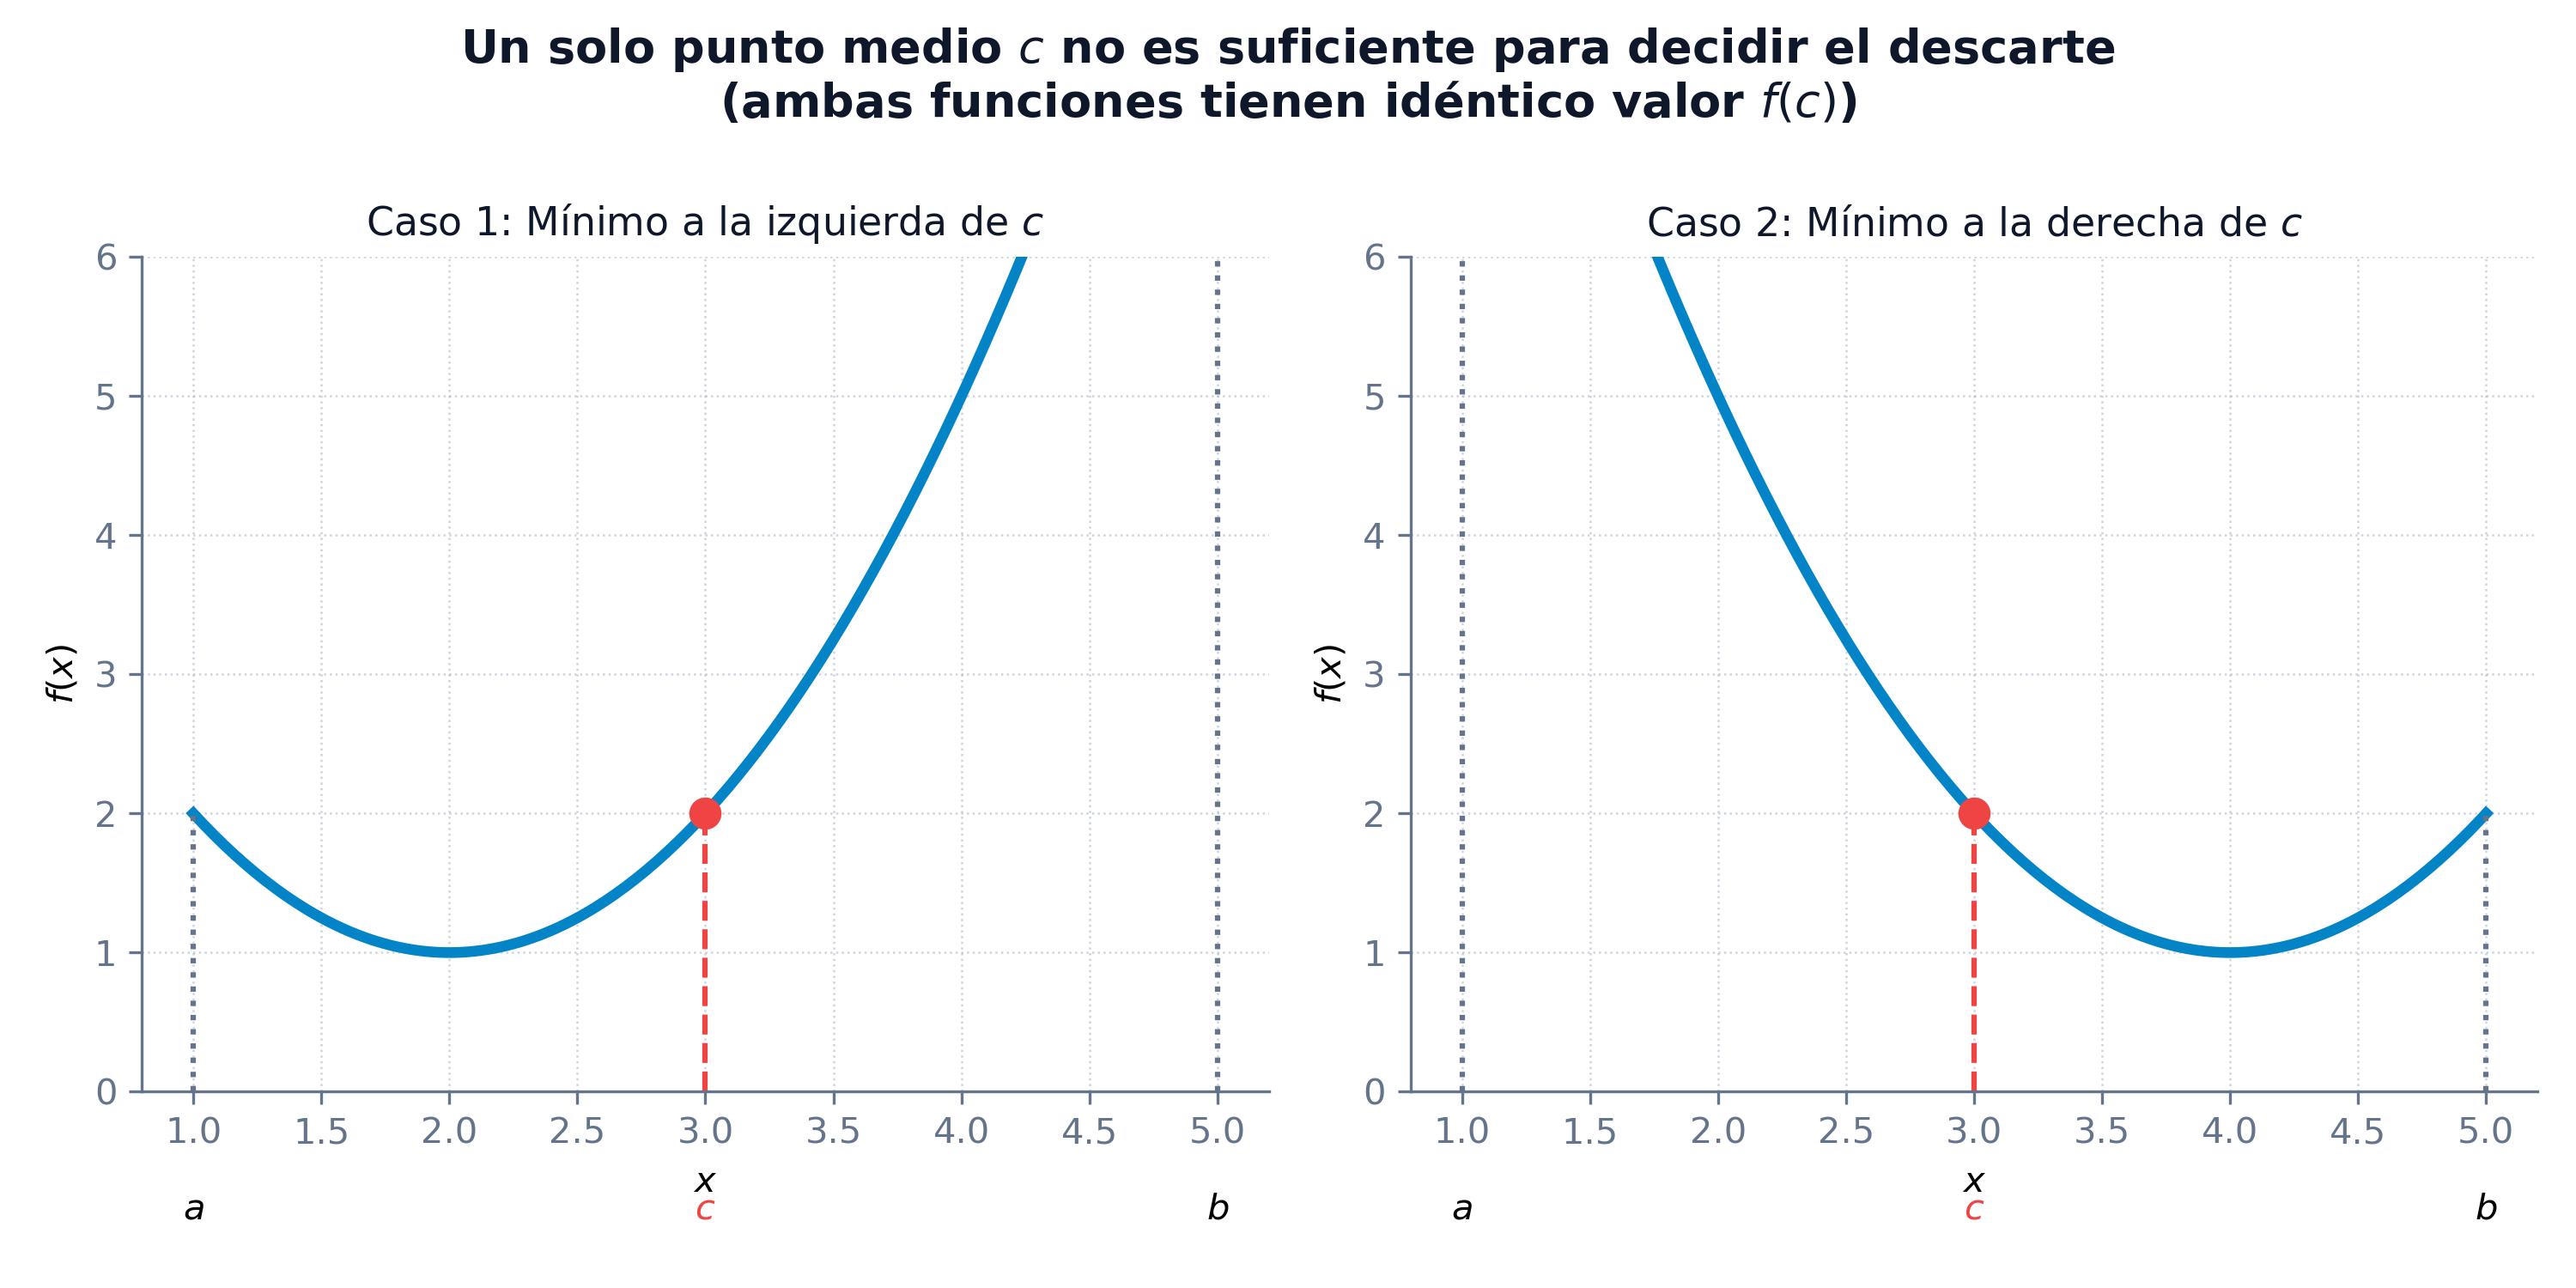
\includegraphics[width=0.95\linewidth,height=\textheight,keepaspectratio]{images/busqueda_dicotomica_insuficiente.png}

}

\caption{\label{fig-busqueda-dicotomica-insuficiente}Insuficiencia de
evaluar un único punto medio: dos funciones unimodales diferentes pueden
tener idéntico valor en \(c\) teniendo sus mínimos globales en lados
opuestos}

\end{figure}%

Para resolver esto, calculamos en cada iteración \(k\) dos puntos
simétricos respecto al punto medio, separados por una perturbación
infinitesimal \(\delta > 0\):
\[\lambda_k = \frac{a_k + b_k}{2} - \delta \qquad \mu_k = \frac{a_k + b_k}{2} + \delta\]
Comparamos sus valores para actualizar el intervalo:

\begin{itemize}
\tightlist
\item
  Si \(f(\lambda_k) < f(\mu_k) \implies\) descartamos \([\mu_k, b_k]\),
  y el nuevo intervalo es \([a_{k+1}, b_{k+1}] = [a_k, \mu_k]\).
\item
  Si \(f(\lambda_k) > f(\mu_k) \implies\) descartamos
  \([a_k, \lambda_k]\), y el nuevo intervalo es
  \([a_{k+1}, b_{k+1}] = [\lambda_k, b_k]\).
\end{itemize}

La amplitud del nuevo intervalo viene dada por la ecuación:
\[I_{k+1} = \frac{b_k - a_k}{2} + \delta\] Cada paso reduce el intervalo
de incertidumbre a la mitad más la perturbación
(\(I_{k+1} \approx \frac{1}{2} I_k\)).

\begin{figure}

\centering{

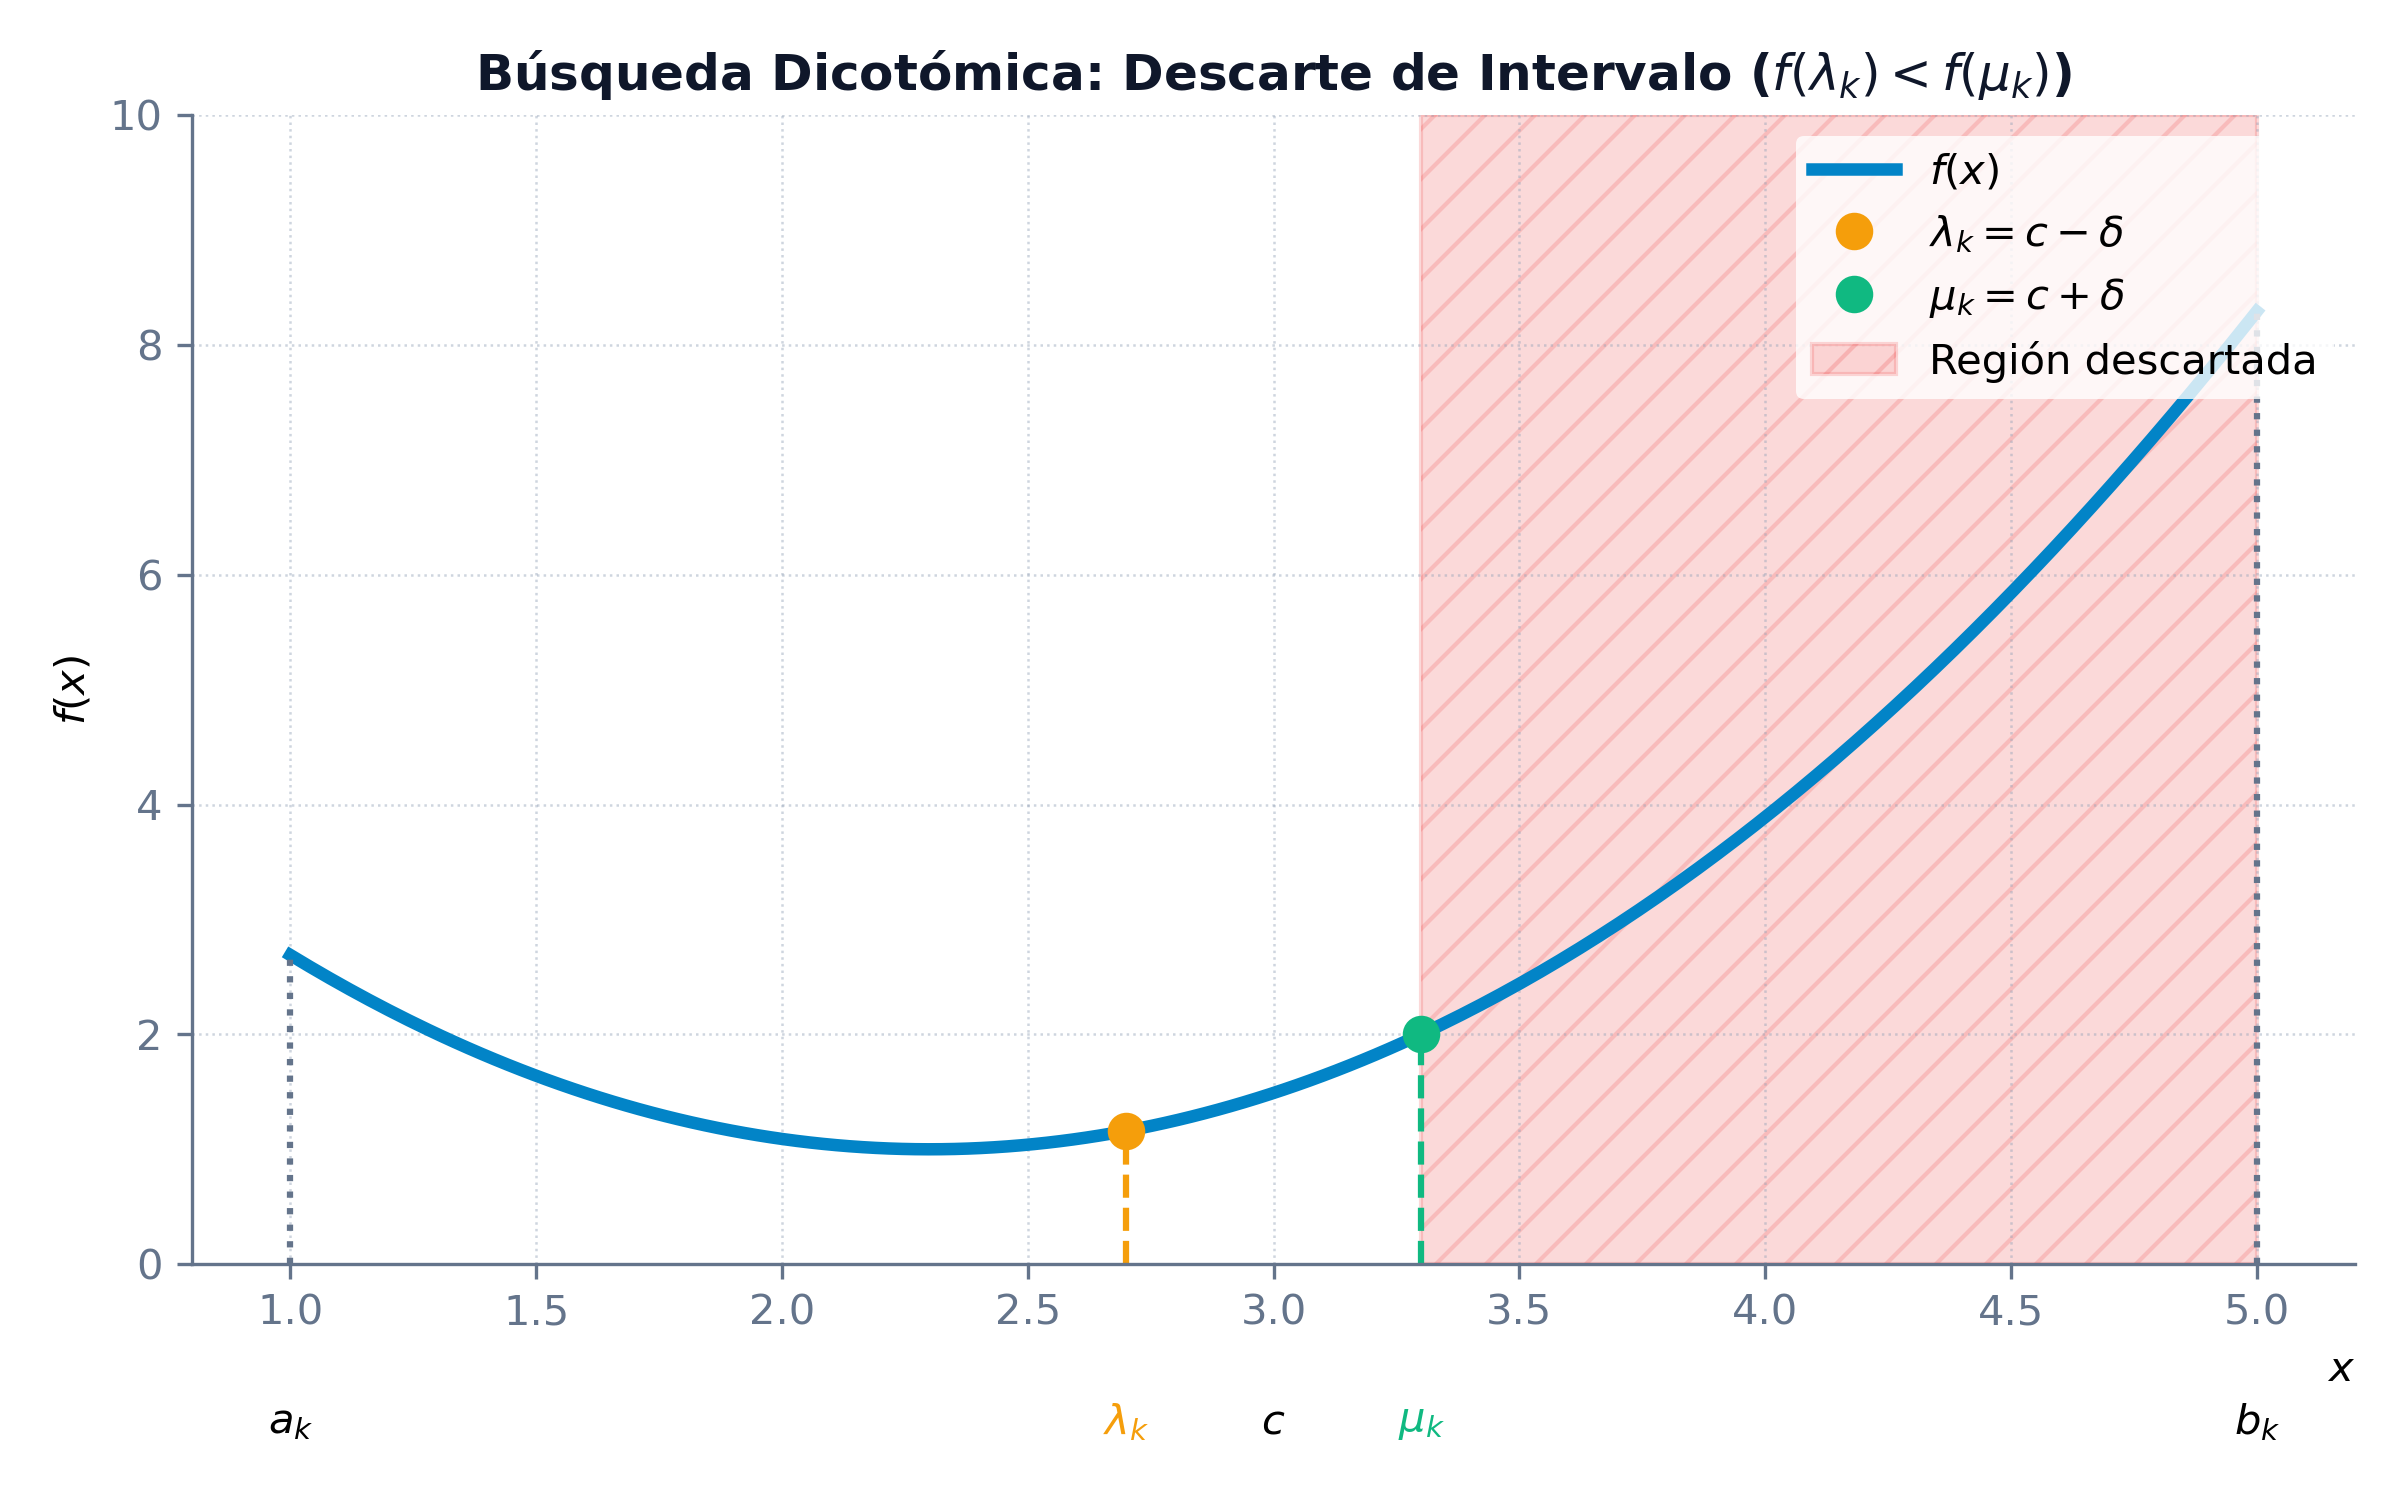
\includegraphics[width=0.7\linewidth,height=\textheight,keepaspectratio]{images/busqueda_dicotomica_concepto.png}

}

\caption{\label{fig-busqueda-dicotomica-concepto}Concepto de la Búsqueda
Dicotómica: la comparación de \(\lambda_k\) y \(\mu_k\) descarta con
certeza una de las mitades del intervalo}

\end{figure}%

\begin{tcolorbox}[enhanced jigsaw, toprule=.15mm, opacitybacktitle=0.6, coltitle=black, colbacktitle=quarto-callout-tip-color!10!white, title=\textcolor{quarto-callout-tip-color}{\faLightbulb}\hspace{0.5em}{Ejemplo: Búsqueda dicotómica}, arc=.35mm, rightrule=.15mm, toptitle=1mm, breakable, bottomtitle=1mm, titlerule=0mm, colback=white, opacityback=0, leftrule=.75mm, colframe=quarto-callout-tip-color-frame, left=2mm, bottomrule=.15mm]

Minimizamos en el intervalo \([1, 4]\) la función de cuarto grado
\(f(x) = \frac{1}{4}x^4 - \frac{13}{3}x^3 + 27x^2 - 72x + 1\) con
perturbación \(\delta = 0.02\) y tolerancia \(\epsilon = 0.15\):

\begin{itemize}
\tightlist
\item
  \textbf{Paso 1}: Intervalo \([a_0, b_0] = [1, 4]\). Punto medio
  \(c = 2.5\).

  \begin{itemize}
  \tightlist
  \item
    Cálculo de puntos internos:
    \[\lambda_0 = \frac{1 + 4}{2} - 0.02 = 2.48 \qquad \mu_0 = \frac{1 + 4}{2} + 0.02 = 2.52\]
  \item
    Evaluaciones correspondientes:
    \[f(2.48) \approx -68.1386 \qquad f(2.52) \approx -68.2437\]
  \item
    Como \(f(\lambda_0) > f(\mu_0)\), descartamos la porción izquierda
    \([1, 2.48]\). Nuevo intervalo: \([a_1, b_1] = [2.48, 4]\).
  \end{itemize}
\item
  \textbf{Paso 2}: Intervalo \([a_1, b_1] = [2.48, 4]\). Punto medio
  \(c = 3.24\).

  \begin{itemize}
  \tightlist
  \item
    Cálculo de puntos internos:
    \[\lambda_1 = \frac{2.48 + 4}{2} - 0.02 = 3.22 \qquad \mu_1 = \frac{2.48 + 4}{2} + 0.02 = 3.26\]
  \item
    Evaluaciones correspondientes:
    \[f(3.22) \approx -68.6910 \qquad f(3.26) \approx -68.6709\]
  \item
    Como \(f(\lambda_1) < f(\mu_1)\), descartamos la porción derecha
    \([3.26, 4]\). Nuevo intervalo: \([a_2, b_2] = [2.48, 3.26]\).
  \end{itemize}
\item
  \textbf{Paso 3}: Intervalo \([a_2, b_2] = [2.48, 3.26]\). Punto medio
  \(c = 2.87\).

  \begin{itemize}
  \tightlist
  \item
    Cálculo de puntos internos:
    \[\lambda_2 = \frac{2.48 + 3.26}{2} - 0.02 = 2.85 \qquad \mu_2 = \frac{2.48 + 3.26}{2} + 0.02 = 2.89\]
  \item
    Evaluaciones correspondientes:
    \[f(2.85) \approx -68.7116 \qquad f(2.89) \approx -68.7300\]
  \item
    Como \(f(\lambda_2) > f(\mu_2)\), descartamos la porción izquierda
    \([2.48, 2.85]\). Nuevo intervalo: \([a_3, b_3] = [2.85, 3.26]\).
  \end{itemize}
\item
  \textbf{Pasos siguientes}: El proceso continúa evaluando de forma
  pareada. En el paso 5, el intervalo se reduce a \([2.9425, 3.075]\)
  con amplitud \(0.1325 \le 0.15\), finalizando el algoritmo.
\end{itemize}

\begin{figure}[H]

\centering{

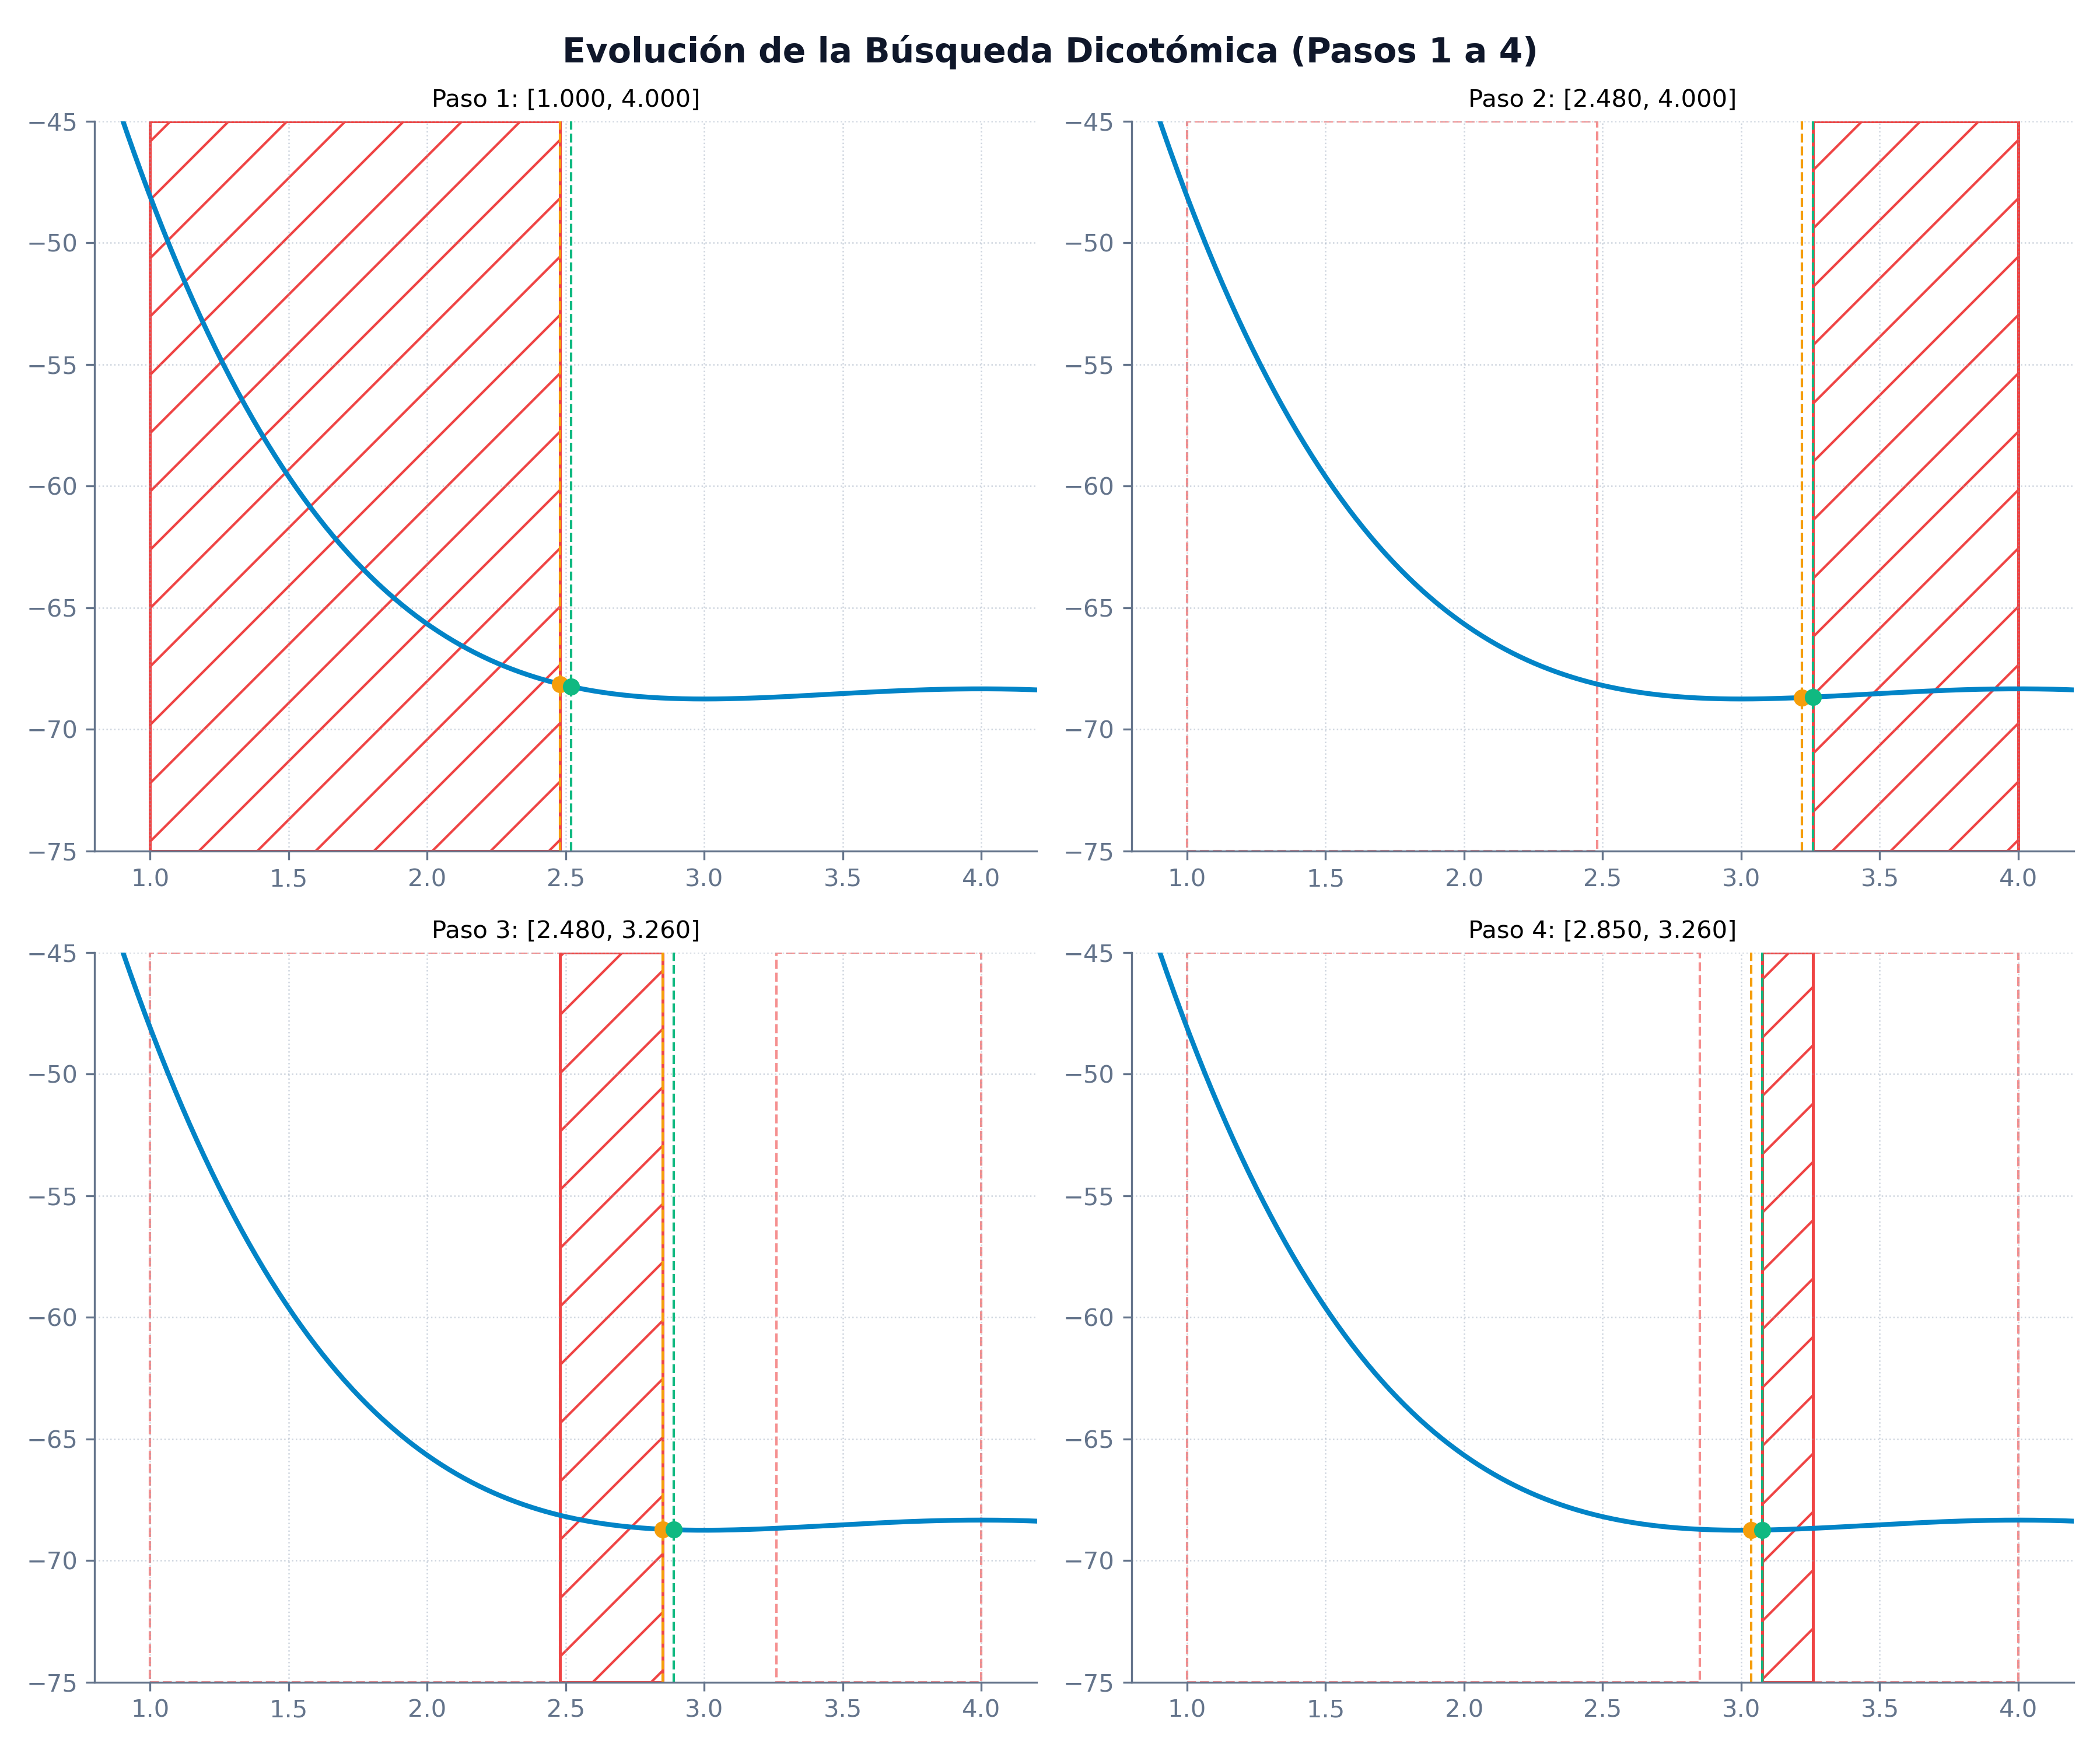
\includegraphics[width=0.85\linewidth,height=\textheight,keepaspectratio]{images/dicotomica_pasos.png}

}

\caption{\label{fig-dicotomica}Evolución del intervalo en la Búsqueda
Dicotómica (Pasos 1 a 4)}

\end{figure}%

\end{tcolorbox}

La \textbf{Sección Áurea (Golden Section)} optimiza la búsqueda
dicotómica reduciendo a la mitad el número de evaluaciones necesarias en
cada paso. Esto se logra colocando los puntos internos \(\lambda_k\) y
\(\mu_k\) de tal forma que uno de ellos coincida exactamente con un
punto evaluado en la iteración anterior, requiriendo solo una nueva
evaluación por iteración a partir de la segunda.

Para deducir la razón áurea \(\alpha > 1\), consideremos la proporción
constante entre la amplitud de intervalos consecutivos:
\[I_k = \alpha \cdot I_{k+1} \qquad I_{k+1} = \alpha \cdot I_{k+2} \implies I_k = \alpha^2 \cdot I_{k+2}\]
Dado que los puntos se sitúan de manera simétrica, la longitud total del
intervalo actual \(I_k\) es la suma de los dos posibles subintervalos
sucesivos \(I_{k+1}\) y \(I_{k+2}\): \[I_k = I_{k+1} + I_{k+2}\]
Sustituyendo las relaciones de escala constante obtenemos:
\[\alpha^2 \cdot I_{k+2} = \alpha \cdot I_{k+2} + I_{k+2} \iff \alpha^2 - \alpha - 1 = 0\]
Tomando la solución positiva de esta ecuación cuadrática obtenemos el
\textbf{número áureo}:
\[\alpha = \frac{1 + \sqrt{5}}{2} \approx 1.618033988\]

Los puntos de evaluación en cada iteración \(k\) sobre el intervalo
\([a_k, b_k]\) se calculan como:
\[\lambda_k = b_k - \frac{b_k - a_k}{\alpha} \qquad \mu_k = a_k + \frac{b_k - a_k}{\alpha}\]
La amplitud decrece en cada paso por un factor de
\(1/\alpha \approx 0.618\). Dada una tolerancia \(\epsilon > 0\) y
amplitud inicial \(I_0 = b - a\), el número total de iteraciones \(N\)
viene dado por:
\[N = \left\lceil \frac{\ln(I_0) - \ln(\epsilon)}{\ln(\alpha)} \right\rceil\]

\begin{tcolorbox}[enhanced jigsaw, toprule=.15mm, opacitybacktitle=0.6, coltitle=black, colbacktitle=quarto-callout-tip-color!10!white, title=\textcolor{quarto-callout-tip-color}{\faLightbulb}\hspace{0.5em}{Ejemplo: Sección áurea}, arc=.35mm, rightrule=.15mm, toptitle=1mm, breakable, bottomtitle=1mm, titlerule=0mm, colback=white, opacityback=0, leftrule=.75mm, colframe=quarto-callout-tip-color-frame, left=2mm, bottomrule=.15mm]

Minimizamos en el intervalo \([1, 4]\) la función
\(f(x) = \frac{1}{4}x^4 - \frac{13}{3}x^3 + 27x^2 - 72x + 1\) con
tolerancia \(\epsilon = 0.15\). El número de iteraciones requerido es
\(N = \lceil (\ln(3.0) - \ln(0.15)) / \ln(1.61803) \rceil = 7\).

\begin{itemize}
\tightlist
\item
  \textbf{Paso 1}: Intervalo inicial \([a_0, b_0] = [1, 4]\). Amplitud
  teórica \(I_1 = 3.0 / 1.61803 \approx 1.8541\).

  \begin{itemize}
  \tightlist
  \item
    Cálculo de puntos y evaluaciones:
    \[\lambda_0 = 4 - 1.8541 = 2.1459 \implies f(2.1459) \approx -66.692\]
    \[\mu_0 = 1 + 1.8541 = 2.8541 \implies f(2.8541) \approx -68.714\]
  \item
    Como \(f(\lambda_0) > f(\mu_0)\), descartamos la porción izquierda
    \([1, 2.1459]\). Nuevo intervalo: \([a_1, b_1] = [2.1459, 4]\).
  \end{itemize}
\item
  \textbf{Paso 2}: Intervalo \([a_1, b_1] = [2.1459, 4]\). Amplitud
  \(I_2 = 1.8541 / 1.61803 \approx 1.1459\).

  \begin{itemize}
  \tightlist
  \item
    Reutilizamos el punto interior evaluado previamente:
    \[\lambda_1 = \mu_0 = 2.8541 \implies f(2.8541) \approx -68.714\]
  \item
    Calculamos únicamente el nuevo punto y su evaluación:
    \[\mu_1 = 2.1459 + 1.1459 = 3.2918 \implies f(3.2918) \approx -68.654\]
  \item
    Como \(f(\lambda_1) < f(\mu_1)\), descartamos la derecha
    \([3.2918, 4]\). Nuevo intervalo: \([a_2, b_2] = [2.1459, 3.2918]\).
  \end{itemize}
\item
  \textbf{Paso 3}: Intervalo \([a_2, b_2] = [2.1459, 3.2918]\). Amplitud
  \(I_3 = 1.1459 / 1.61803 \approx 0.7082\).

  \begin{itemize}
  \tightlist
  \item
    Reutilizamos el punto interior:
    \[\mu_2 = \lambda_1 = 2.8541 \implies f(2.8541) \approx -68.714\]
  \item
    Calculamos el nuevo punto:
    \[\lambda_2 = 3.2918 - 0.7082 = 2.5836 \implies f(2.5836) \approx -68.3861\]
  \item
    Como \(f(\lambda_2) > f(\mu_2)\), descartamos la izquierda
    \([2.1459, 2.5836]\). Nuevo intervalo:
    \([a_3, b_3] = [2.5836, 3.2918]\).
  \end{itemize}
\item
  \textbf{Pasos siguientes}: El algoritmo continúa reutilizando
  evaluaciones previas de forma simétrica. En el paso 7, la amplitud
  alcanza \(0.1033 \le 0.15\) convergiendo al intervalo final
  \([2.9574, 3.0608]\), el cual contiene el mínimo analítico en
  \(x^* = 3.0\).
\end{itemize}

\begin{figure}[H]

\centering{

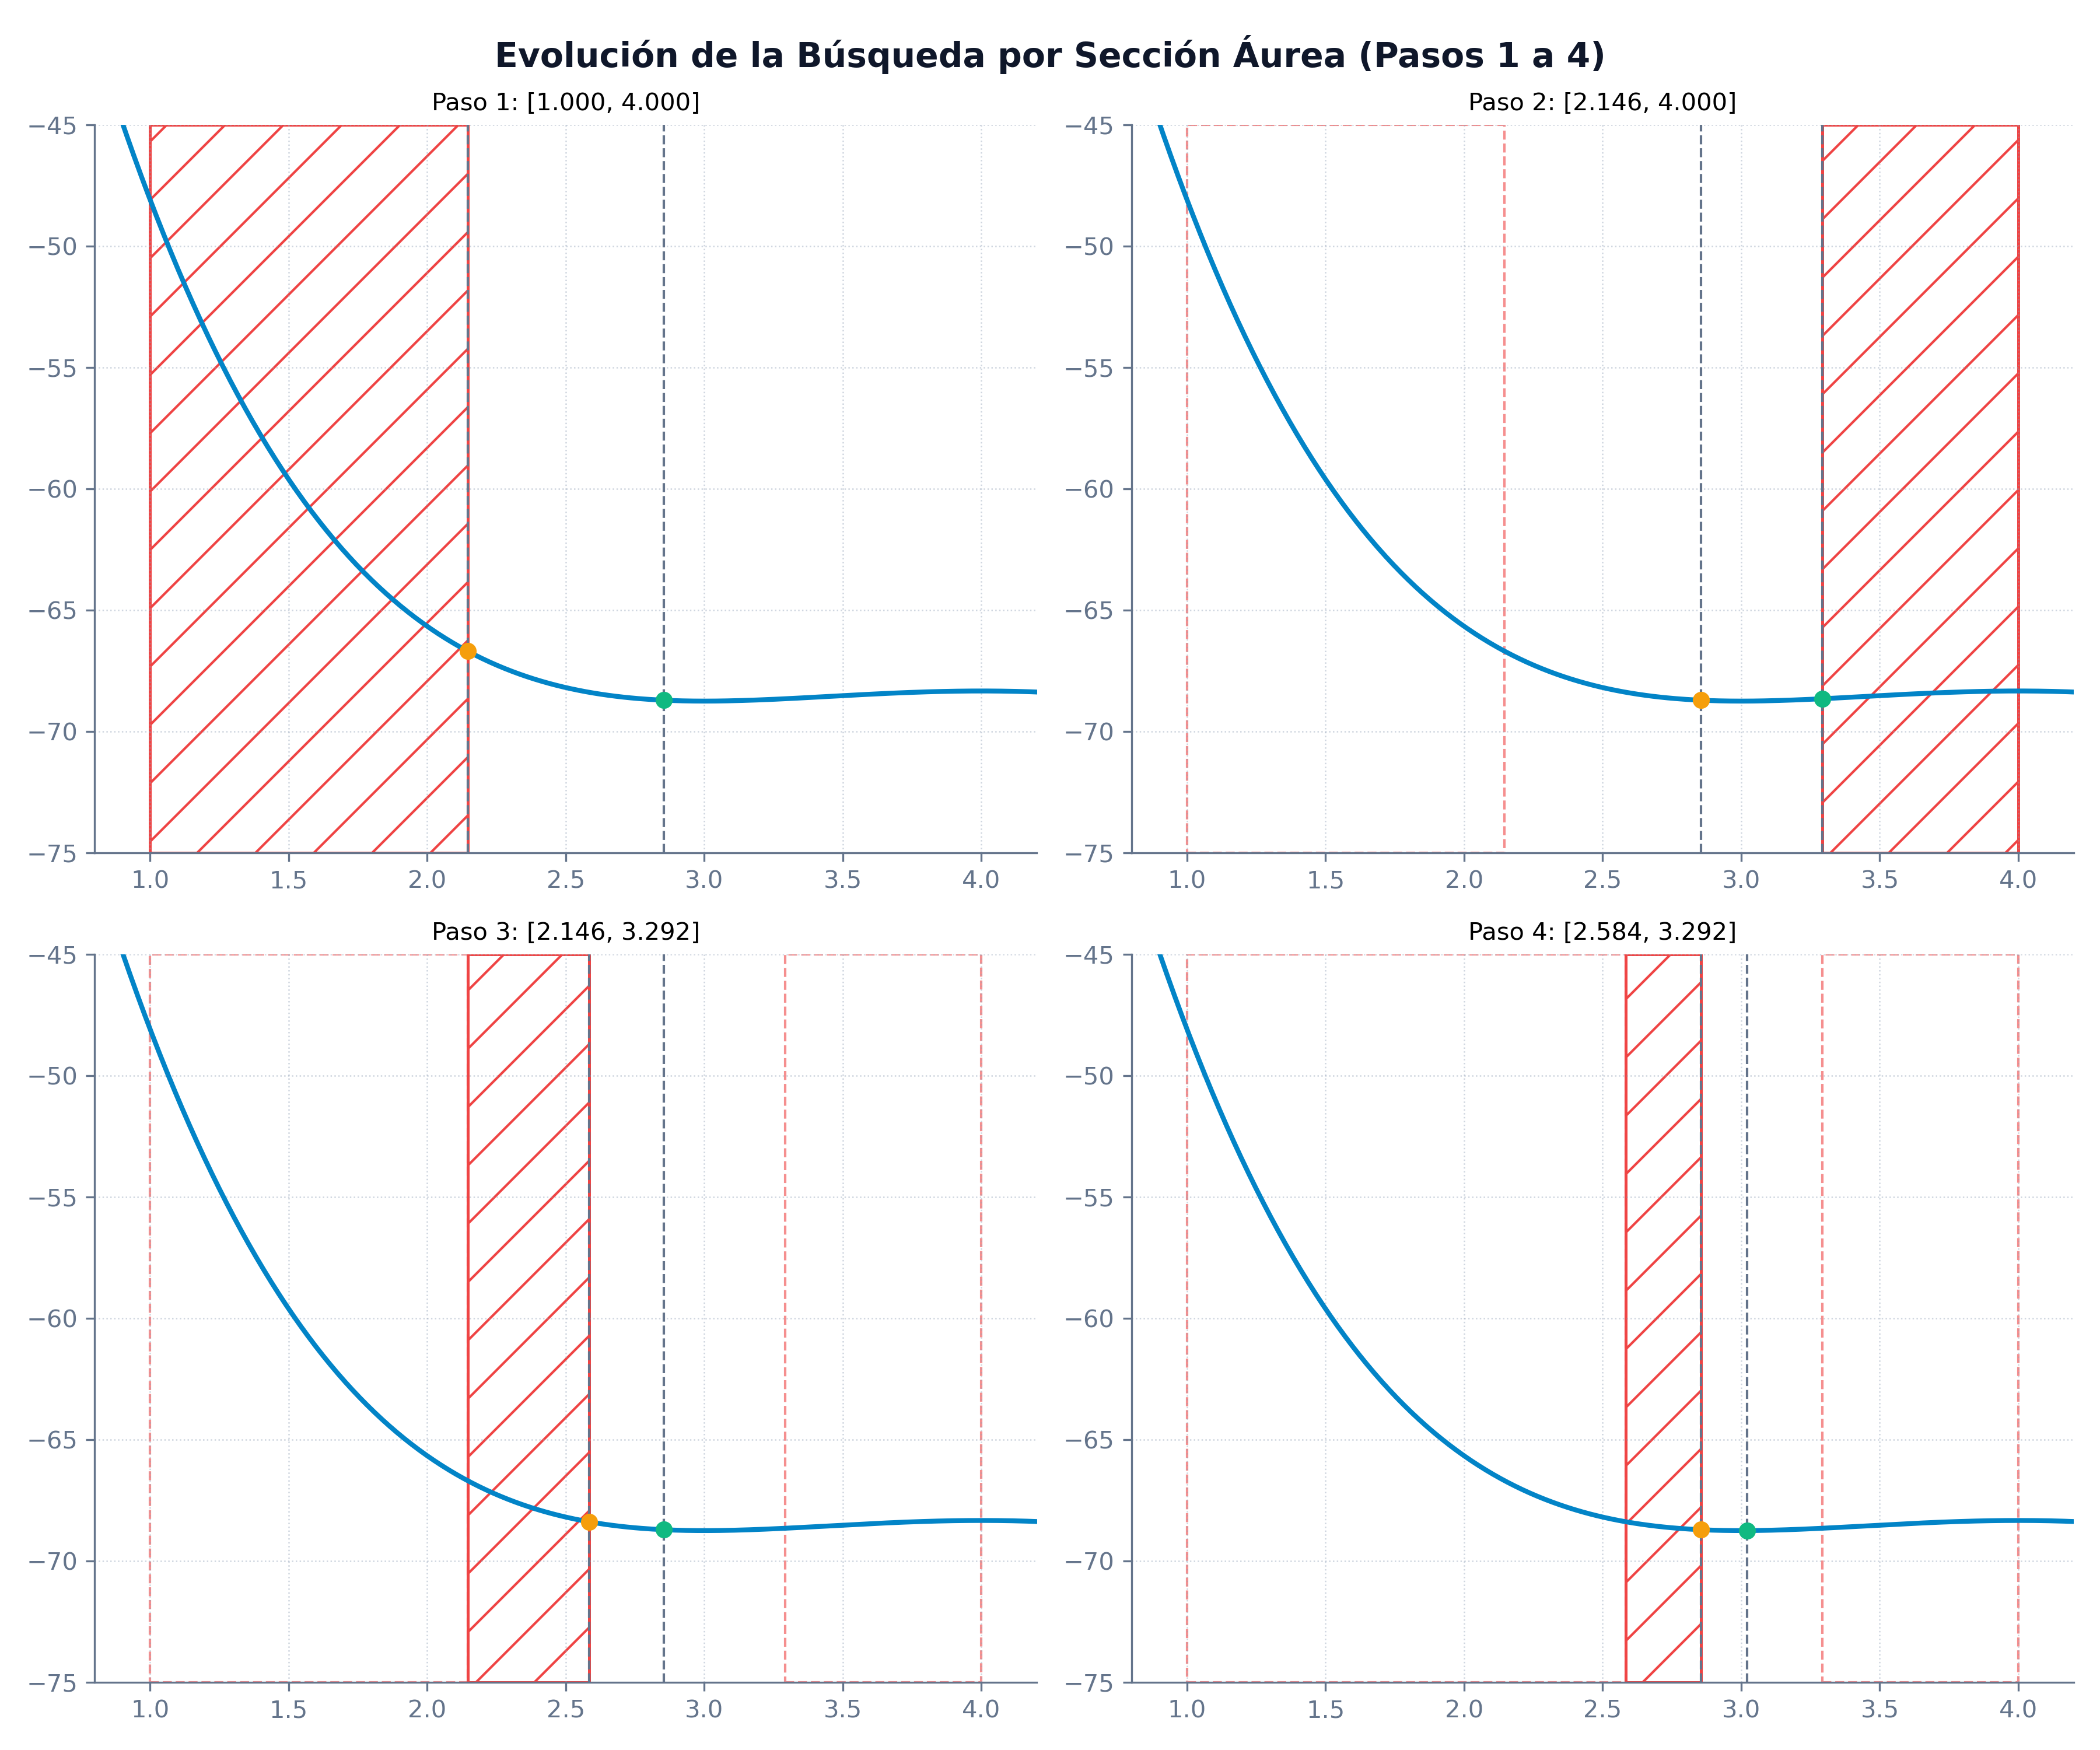
\includegraphics[width=0.85\linewidth,height=\textheight,keepaspectratio]{images/seccion_aurea_pasos.png}

}

\caption{\label{fig-seccion-aurea}Evolución del intervalo en la búsqueda
por Sección Áurea (Pasos 1 a 4)}

\end{figure}%

\end{tcolorbox}

La \textbf{Búsqueda de Fibonacci} optimiza teóricamente la sección áurea
si se fija de antemano el número total de evaluaciones de la función
\(N\). Utiliza los términos de la sucesión de Fibonacci (\(F_i\), donde
\(F_0=1, F_1=1, F_2=2, F_3=3, F_4=5, F_5=8, F_6=13, F_7=21, \dots\)
definidos por recurrencia \(F_i = F_{i-1} + F_{i-2}\)) para calcular la
amplitud del paso en cada iteración \(k\):
\[I_k = \frac{F_{N-k}}{F_{N-k+2}} (b_{k-1} - a_{k-1})\]

A partir de estas amplitudes, los puntos de evaluación se definen en la
iteración \(k\) de la forma:
\[\mu_k = a_k + \frac{F_{N-k}}{F_{N-k+1}} (b_k - a_k) \qquad \lambda_k = a_k + \frac{F_{N-k-1}}{F_{N-k+1}} (b_k - a_k)\]
Al igual que en la Sección Áurea, las amplitudes de intervalos sucesivos
guardan la relación de suma \(I_{k-1} = I_k + I_{k+1}\), lo que permite
reutilizar un punto evaluado en cada iteración. En el paso final
\(k=N-1\), ambos puntos coinciden en el centro del intervalo,
requiriendo introducir una pequeña perturbación \(\epsilon_0 > 0\) para
poder tomar la decisión de descarte definitiva. Aunque Fibonacci
proporciona la máxima reducción matemática en un número de pasos fijo,
la Sección Áurea es preferible habitualmente porque no requiere
predeterminar \(N\) ni almacenar o calcular la sucesión de Fibonacci.

\begin{tcolorbox}[enhanced jigsaw, toprule=.15mm, opacitybacktitle=0.6, coltitle=black, colbacktitle=quarto-callout-tip-color!10!white, title=\textcolor{quarto-callout-tip-color}{\faLightbulb}\hspace{0.5em}{Ejemplo: Búsqueda de Fibonacci}, arc=.35mm, rightrule=.15mm, toptitle=1mm, breakable, bottomtitle=1mm, titlerule=0mm, colback=white, opacityback=0, leftrule=.75mm, colframe=quarto-callout-tip-color-frame, left=2mm, bottomrule=.15mm]

Minimizamos la misma función en \([1, 4]\) con tolerancia
\(\epsilon = 0.15\) fijando un número total de evaluaciones \(N = 6\)
(usando \(F_7 = 21\)).

\begin{itemize}
\tightlist
\item
  \textbf{Paso 1}: Intervalo inicial \([a_0, b_0] = [1, 4]\).

  \begin{itemize}
  \tightlist
  \item
    Amplitud teórica del paso:
    \[I_1 = \frac{F_6}{F_7}(b_0 - a_0) = \frac{13}{21} \cdot 3.0 \approx 1.8571\]
  \item
    Cálculo de puntos y evaluaciones:
    \[\lambda_0 = 4 - 1.8571 = 2.1429 \implies f(2.1429) \approx -66.673\]
    \[\mu_0 = 1 + 1.8571 = 2.8571 \implies f(2.8571) \approx -68.715\]
  \item
    Como \(f(\lambda_0) > f(\mu_0)\), descartamos la porción izquierda
    \([1, 2.1429]\). Nuevo intervalo: \([a_1, b_1] = [2.1429, 4]\).
  \end{itemize}
\item
  \textbf{Paso 2}: Intervalo \([a_1, b_1] = [2.1429, 4]\).

  \begin{itemize}
  \tightlist
  \item
    Amplitud teórica:
    \[I_2 = \frac{F_5}{F_7}(b_0 - a_0) = \frac{8}{21} \cdot 3.0 \approx 1.1429\]
  \item
    Reutilizamos el punto evaluado previamente:
    \[\lambda_1 = \mu_0 = 2.8571 \implies f(2.8571) \approx -68.715\]
  \item
    Calculamos el nuevo punto y su evaluación:
    \[\mu_1 = 2.1429 + 1.1429 = 3.2857 \implies f(3.2857) \approx -68.657\]
  \item
    Como \(f(\lambda_1) < f(\mu_1)\), descartamos la derecha
    \([3.2857, 4]\). Nuevo intervalo: \([a_2, b_2] = [2.1429, 3.2857]\).
  \end{itemize}
\item
  \textbf{Pasos siguientes}: Continuando con el proceso de reducción
  mediante los cocientes de Fibonacci, en la iteración 6 (última) la
  amplitud del intervalo alcanza \(I_6 = 0.1429 \le 0.15\), logrando
  converger en el intervalo final \([2.8541, 3.001]\) con una iteración
  menos que en la sección áurea gracias a fijar \(N\) de forma
  anticipada.
\end{itemize}

\end{tcolorbox}

\begin{center}\rule{0.5\linewidth}{0.5pt}\end{center}

\subsection{Métodos con derivadas}\label{muxe9todos-con-derivadas}

Los métodos con derivadas incorporan información analítica de las
pendientes locales para acelerar significativamente la convergencia.

El \textbf{Método de Bisección (Bolzano)} se basa en buscar las raíces
de la derivada de primer orden (\(f'(x) = 0\)). Exige que los signos de
la derivada en los extremos del intervalo inicial \([a_0, b_0]\) sean
opuestos (\(f'(a_0) < 0\) y \(f'(b_0) > 0\)), lo que por el Teorema de
Bolzano asegura la existencia de al menos un punto estacionario en el
interior.

En cada iteración \(k\), calculamos el punto medio:
\[c_k = \frac{a_k + b_k}{2}\] y evaluamos el signo de la derivada en
dicho punto:

\begin{itemize}
\tightlist
\item
  Si \(f'(c_k) < 0 \implies\) actualizamos la cota izquierda:
  \([a_{k+1}, b_{k+1}] = [c_k, b_k]\).
\item
  Si \(f'(c_k) > 0 \implies\) actualizamos la cota derecha:
  \([a_{k+1}, b_{k+1}] = [a_k, c_k]\).
\item
  Si \(f'(c_k) = 0 \implies c_k\) es el punto óptimo exacto.
\end{itemize}

La amplitud del intervalo se reduce a la mitad exacta en cada paso:
\[I_{k+1} = \frac{b_k - a_k}{2}\] El número de pasos \(n\) requeridos
para alcanzar una tolerancia \(\epsilon > 0\) es:
\[n = \left\lceil \frac{\ln(I_0) - \ln(\epsilon)}{\ln(2)} \right\rceil\]

\begin{tcolorbox}[enhanced jigsaw, toprule=.15mm, opacitybacktitle=0.6, coltitle=black, colbacktitle=quarto-callout-tip-color!10!white, title=\textcolor{quarto-callout-tip-color}{\faLightbulb}\hspace{0.5em}{Ejemplo: Método de bisección}, arc=.35mm, rightrule=.15mm, toptitle=1mm, breakable, bottomtitle=1mm, titlerule=0mm, colback=white, opacityback=0, leftrule=.75mm, colframe=quarto-callout-tip-color-frame, left=2mm, bottomrule=.15mm]

Minimizamos en el intervalo \([1, 4]\) la función
\(f(x) = \frac{1}{4}x^4 - \frac{13}{3}x^3 + 27x^2 - 72x + 1\) con
tolerancia \(\epsilon = 0.15\). La primera derivada es
\(f'(x) = x^3 - 13x^2 + 54x - 72\).

\begin{itemize}
\tightlist
\item
  \textbf{Paso 1}: Intervalo inicial \([a_0, b_0] = [1, 4]\).

  \begin{itemize}
  \tightlist
  \item
    Calculamos el punto medio: \[c_0 = \frac{1 + 4}{2} = 2.5\]
  \item
    Evaluamos la derivada en \(c_0\):
    \[f'(2.5) = (2.5)^3 - 13(2.5)^2 + 54(2.5) - 72 = -2.6250 < 0\]
  \item
    Como \(f'(2.5) < 0\), descartamos la izquierda. Nuevo intervalo:
    \([a_1, b_1] = [2.5, 4]\).
  \end{itemize}
\item
  \textbf{Paso 2}: Intervalo \([a_1, b_1] = [2.5, 4]\).

  \begin{itemize}
  \tightlist
  \item
    Punto medio: \[c_1 = \frac{2.5 + 4}{2} = 3.25\]
  \item
    Evaluamos la derivada en \(c_1\):
    \[f'(3.25) = (3.25)^3 - 13(3.25)^2 + 54(3.25) - 72 = 0.5156 > 0\]
  \item
    Como \(f'(3.25) > 0\), descartamos la derecha. Nuevo intervalo:
    \([a_2, b_2] = [2.5, 3.25]\).
  \end{itemize}
\item
  \textbf{Paso 3}: Intervalo \([a_2, b_2] = [2.5, 3.25]\).

  \begin{itemize}
  \tightlist
  \item
    Punto medio: \[c_2 = \frac{2.5 + 3.25}{2} = 2.875\]
  \item
    Evaluamos la derivada: \[f'(2.875) \approx -0.4395 < 0\]
  \item
    Descartamos la izquierda. Nuevo intervalo:
    \([a_3, b_3] = [2.875, 3.25]\).
  \end{itemize}
\item
  \textbf{Pasos siguientes}: Continuando el proceso de subdivisión, en
  el paso 5 se obtiene el intervalo final \([2.96875, 3.0625]\) con
  amplitud \(0.0938 \le 0.15\), finalizando el algoritmo.
\end{itemize}

\begin{figure}[H]

\centering{

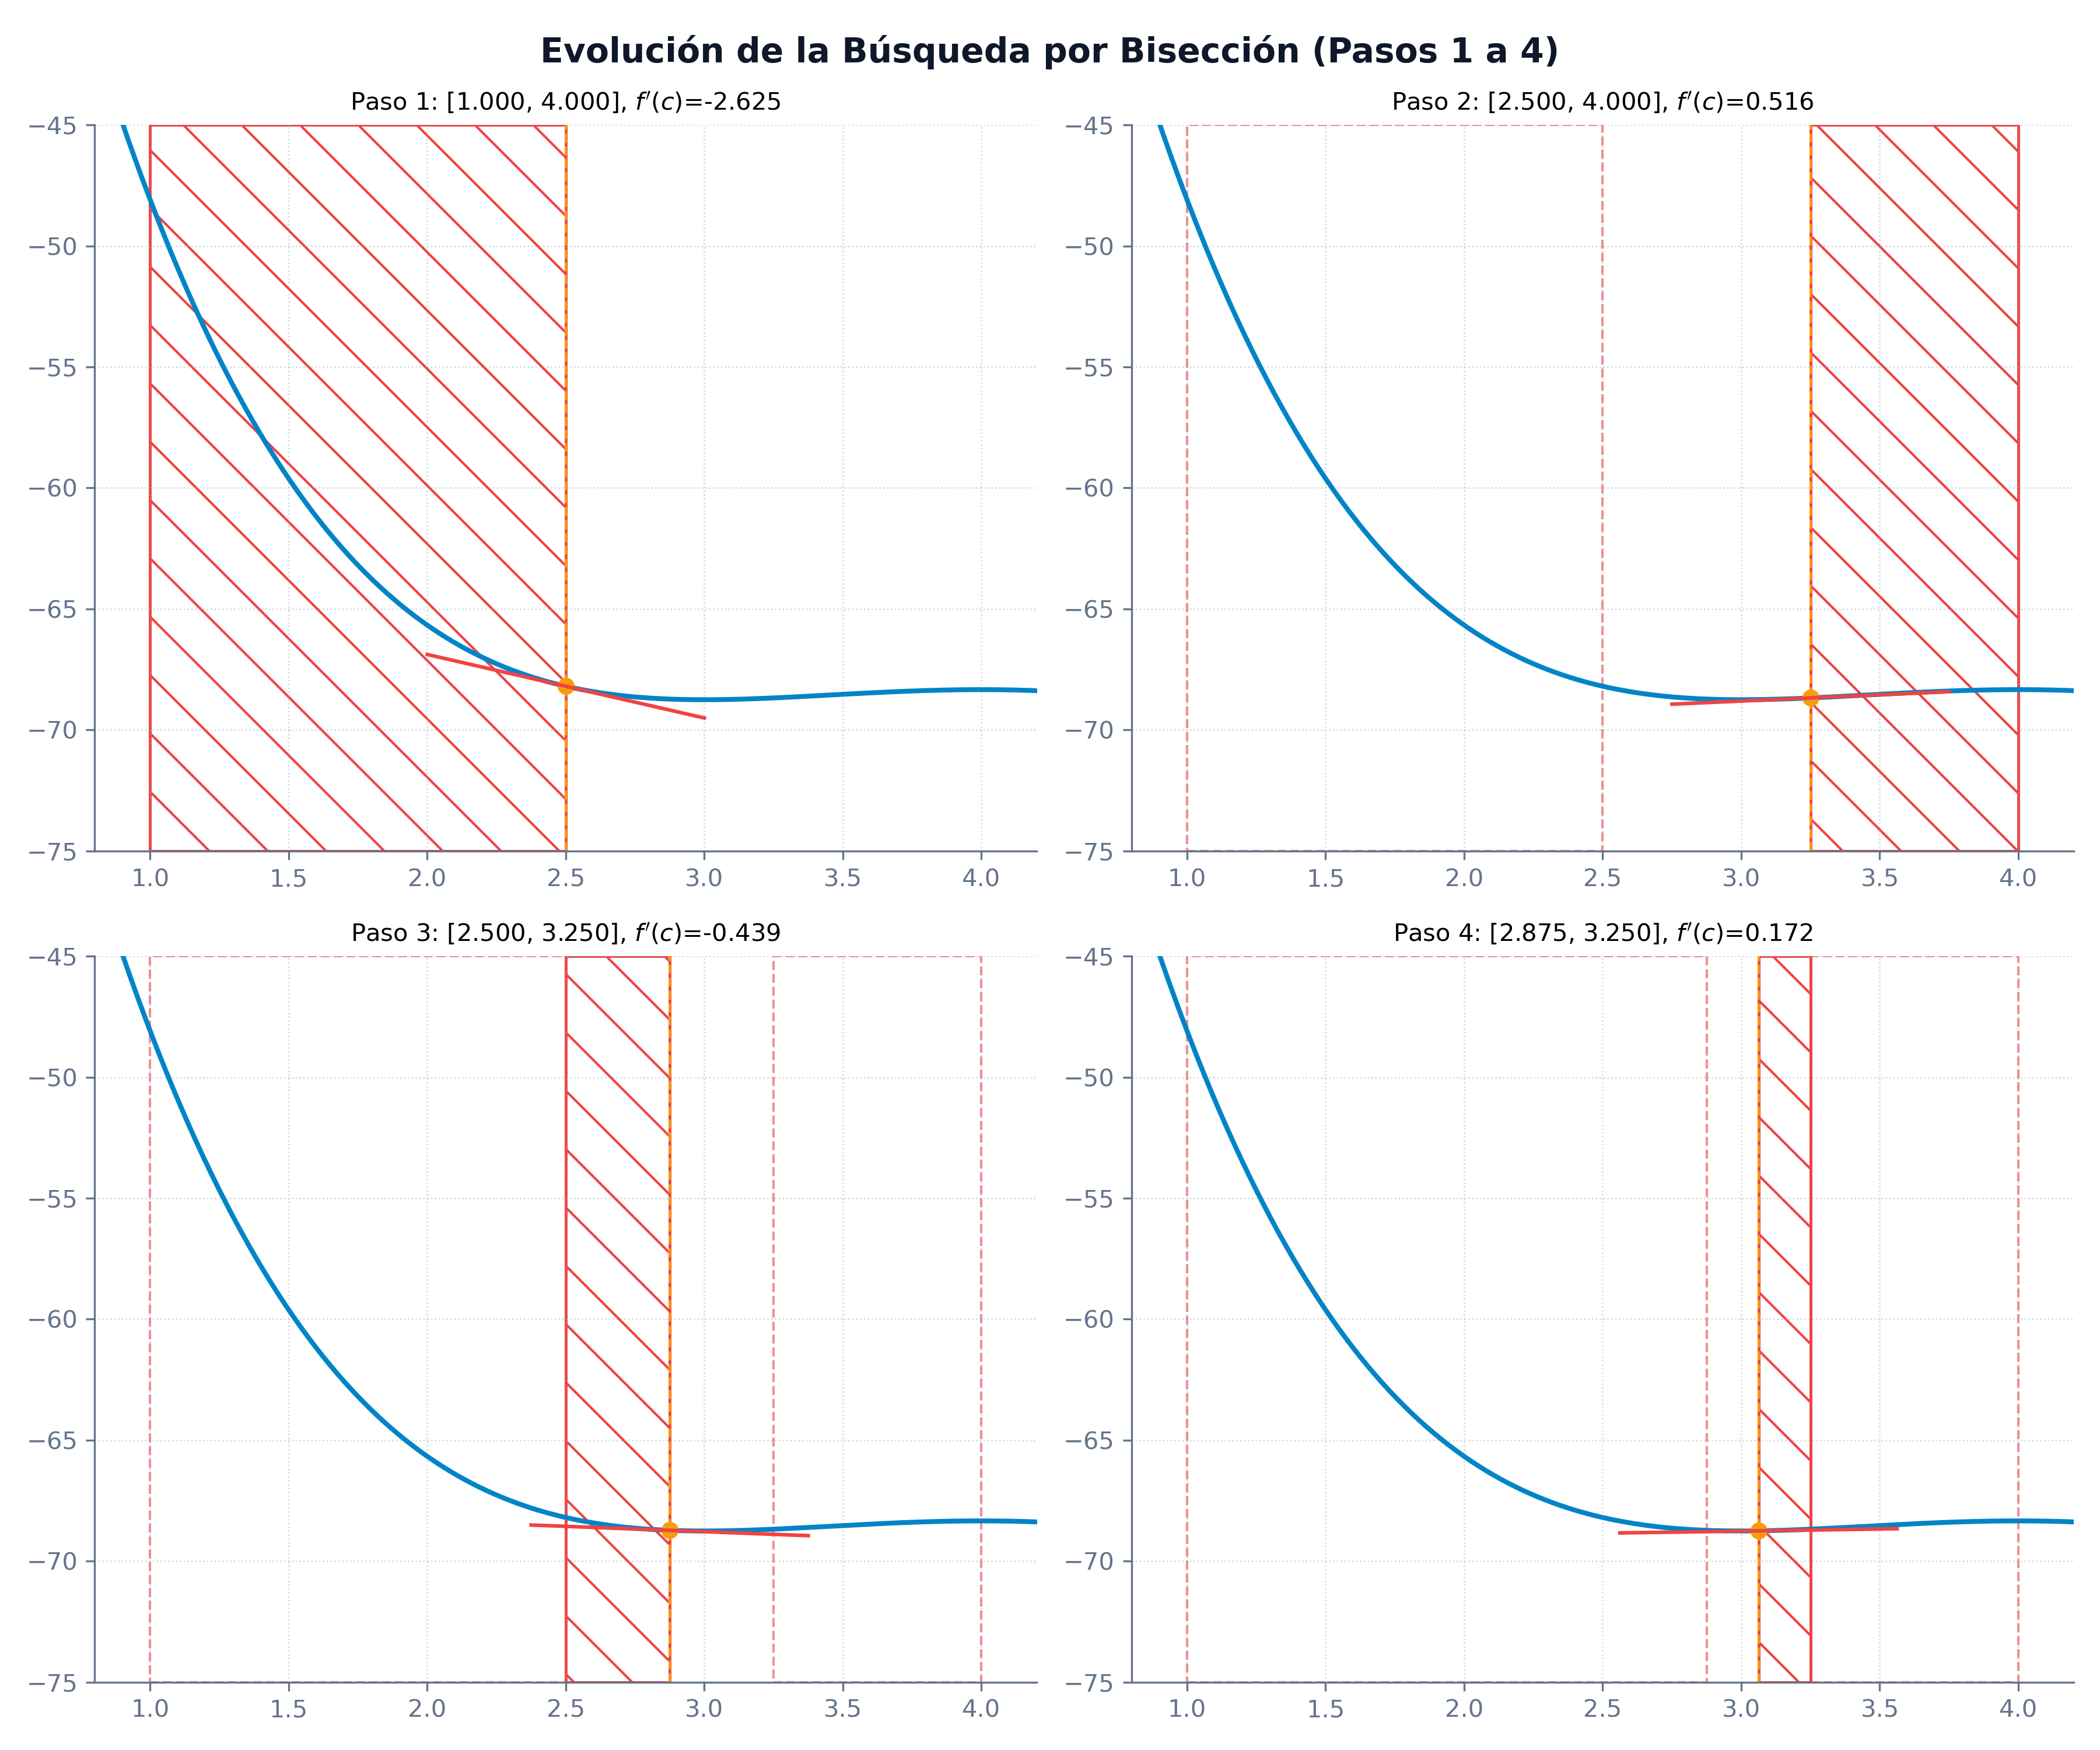
\includegraphics[width=0.85\linewidth,height=\textheight,keepaspectratio]{images/biseccion_pasos.png}

}

\caption{\label{fig-biseccion}Evolución del intervalo en la búsqueda por
Bisección (Pasos 1 a 4)}

\end{figure}%

\end{tcolorbox}

El \textbf{Método de Newton 1D} aproxima localmente la función objetivo
en cada paso \(x_k\) mediante su polinomio cuadrático de Taylor de
segundo orden:
\[q(x) = f(x_k) + f'(x_k)(x - x_k) + \frac{1}{2} f''(x_k)(x - x_k)^2\]
Para encontrar el mínimo de esta aproximación parabólica, igualamos su
derivada a cero:
\[q'(x) = f'(x_k) + f''(x_k)(x - x_k) = 0 \implies x = x_k - \frac{f'(x_k)}{f''(x_k)}\]
Esto nos da la regla iterativa clásica de actualización del método:
\[x_{k+1} = x_k - \frac{f'(x_k)}{f''(x_k)}\] Presenta una
\textbf{convergencia cuadrática local} (orden 2), duplicando el número
de dígitos significativos de precisión en cada paso cuando está cerca
del óptimo. Exige calcular tanto \(f'(x)\) como \(f''(x)\) en cada paso,
requiriendo que la función sea de clase \(\mathcal{C}^2\) y que la
curvatura sea estrictamente positiva (\(f''(x_k) > 0\)).

\begin{tcolorbox}[enhanced jigsaw, toprule=.15mm, opacitybacktitle=0.6, coltitle=black, colbacktitle=quarto-callout-tip-color!10!white, title=\textcolor{quarto-callout-tip-color}{\faLightbulb}\hspace{0.5em}{Ejemplo: Método de Newton 1D}, arc=.35mm, rightrule=.15mm, toptitle=1mm, breakable, bottomtitle=1mm, titlerule=0mm, colback=white, opacityback=0, leftrule=.75mm, colframe=quarto-callout-tip-color-frame, left=2mm, bottomrule=.15mm]

Minimizamos en el intervalo \([1, 4]\) la misma función partiendo de
\(x_0 = 1.0\). Las derivadas son \(f'(x) = x^3 - 13x^2 + 54x - 72\) y
\(f''(x) = 3x^2 - 26x + 54\).

\begin{itemize}
\tightlist
\item
  \textbf{Paso 1}: Partimos de \(x_0 = 1.0\).

  \begin{itemize}
  \tightlist
  \item
    Evaluamos derivadas:
    \[f'(1.0) = 1^3 - 13(1)^2 + 54(1) - 72 = -30.0\]
    \[f''(1.0) = 3(1)^2 - 26(1) + 54 = 31.0\]
  \item
    Actualización: \[x_1 = 1.0 - \frac{-30.0}{31.0} \approx 1.9677\]
  \end{itemize}
\item
  \textbf{Paso 2}: Partimos del punto previo \(x_1 = 1.9677\).

  \begin{itemize}
  \tightlist
  \item
    Evaluamos derivadas:
    \[f'(1.9677) \approx -8.4589 \qquad f''(1.9677) \approx 14.4547\]
  \item
    Actualización:
    \[x_2 = 1.9677 - \frac{-8.4589}{14.4547} \approx 2.5529\]
  \end{itemize}
\item
  \textbf{Paso 3}: Partimos de \(x_2 = 2.5529\).

  \begin{itemize}
  \tightlist
  \item
    Evaluamos derivadas:
    \[f'(2.5529) \approx -2.2300 \qquad f''(2.5529) \approx 7.1760\]
  \item
    Actualización:
    \[x_3 = 2.5529 - \frac{-2.2300}{7.1760} \approx 2.8637\]
  \end{itemize}
\item
  \textbf{Pasos siguientes}: Aplicando de nuevo la fórmula se obtiene
  \(x_4 \approx 2.9808\) y finalmente \(x_5 \approx 2.9995 \approx 3.0\)
  logrando la convergencia óptima en solo 5 iteraciones.
\end{itemize}

\begin{figure}[H]

\centering{

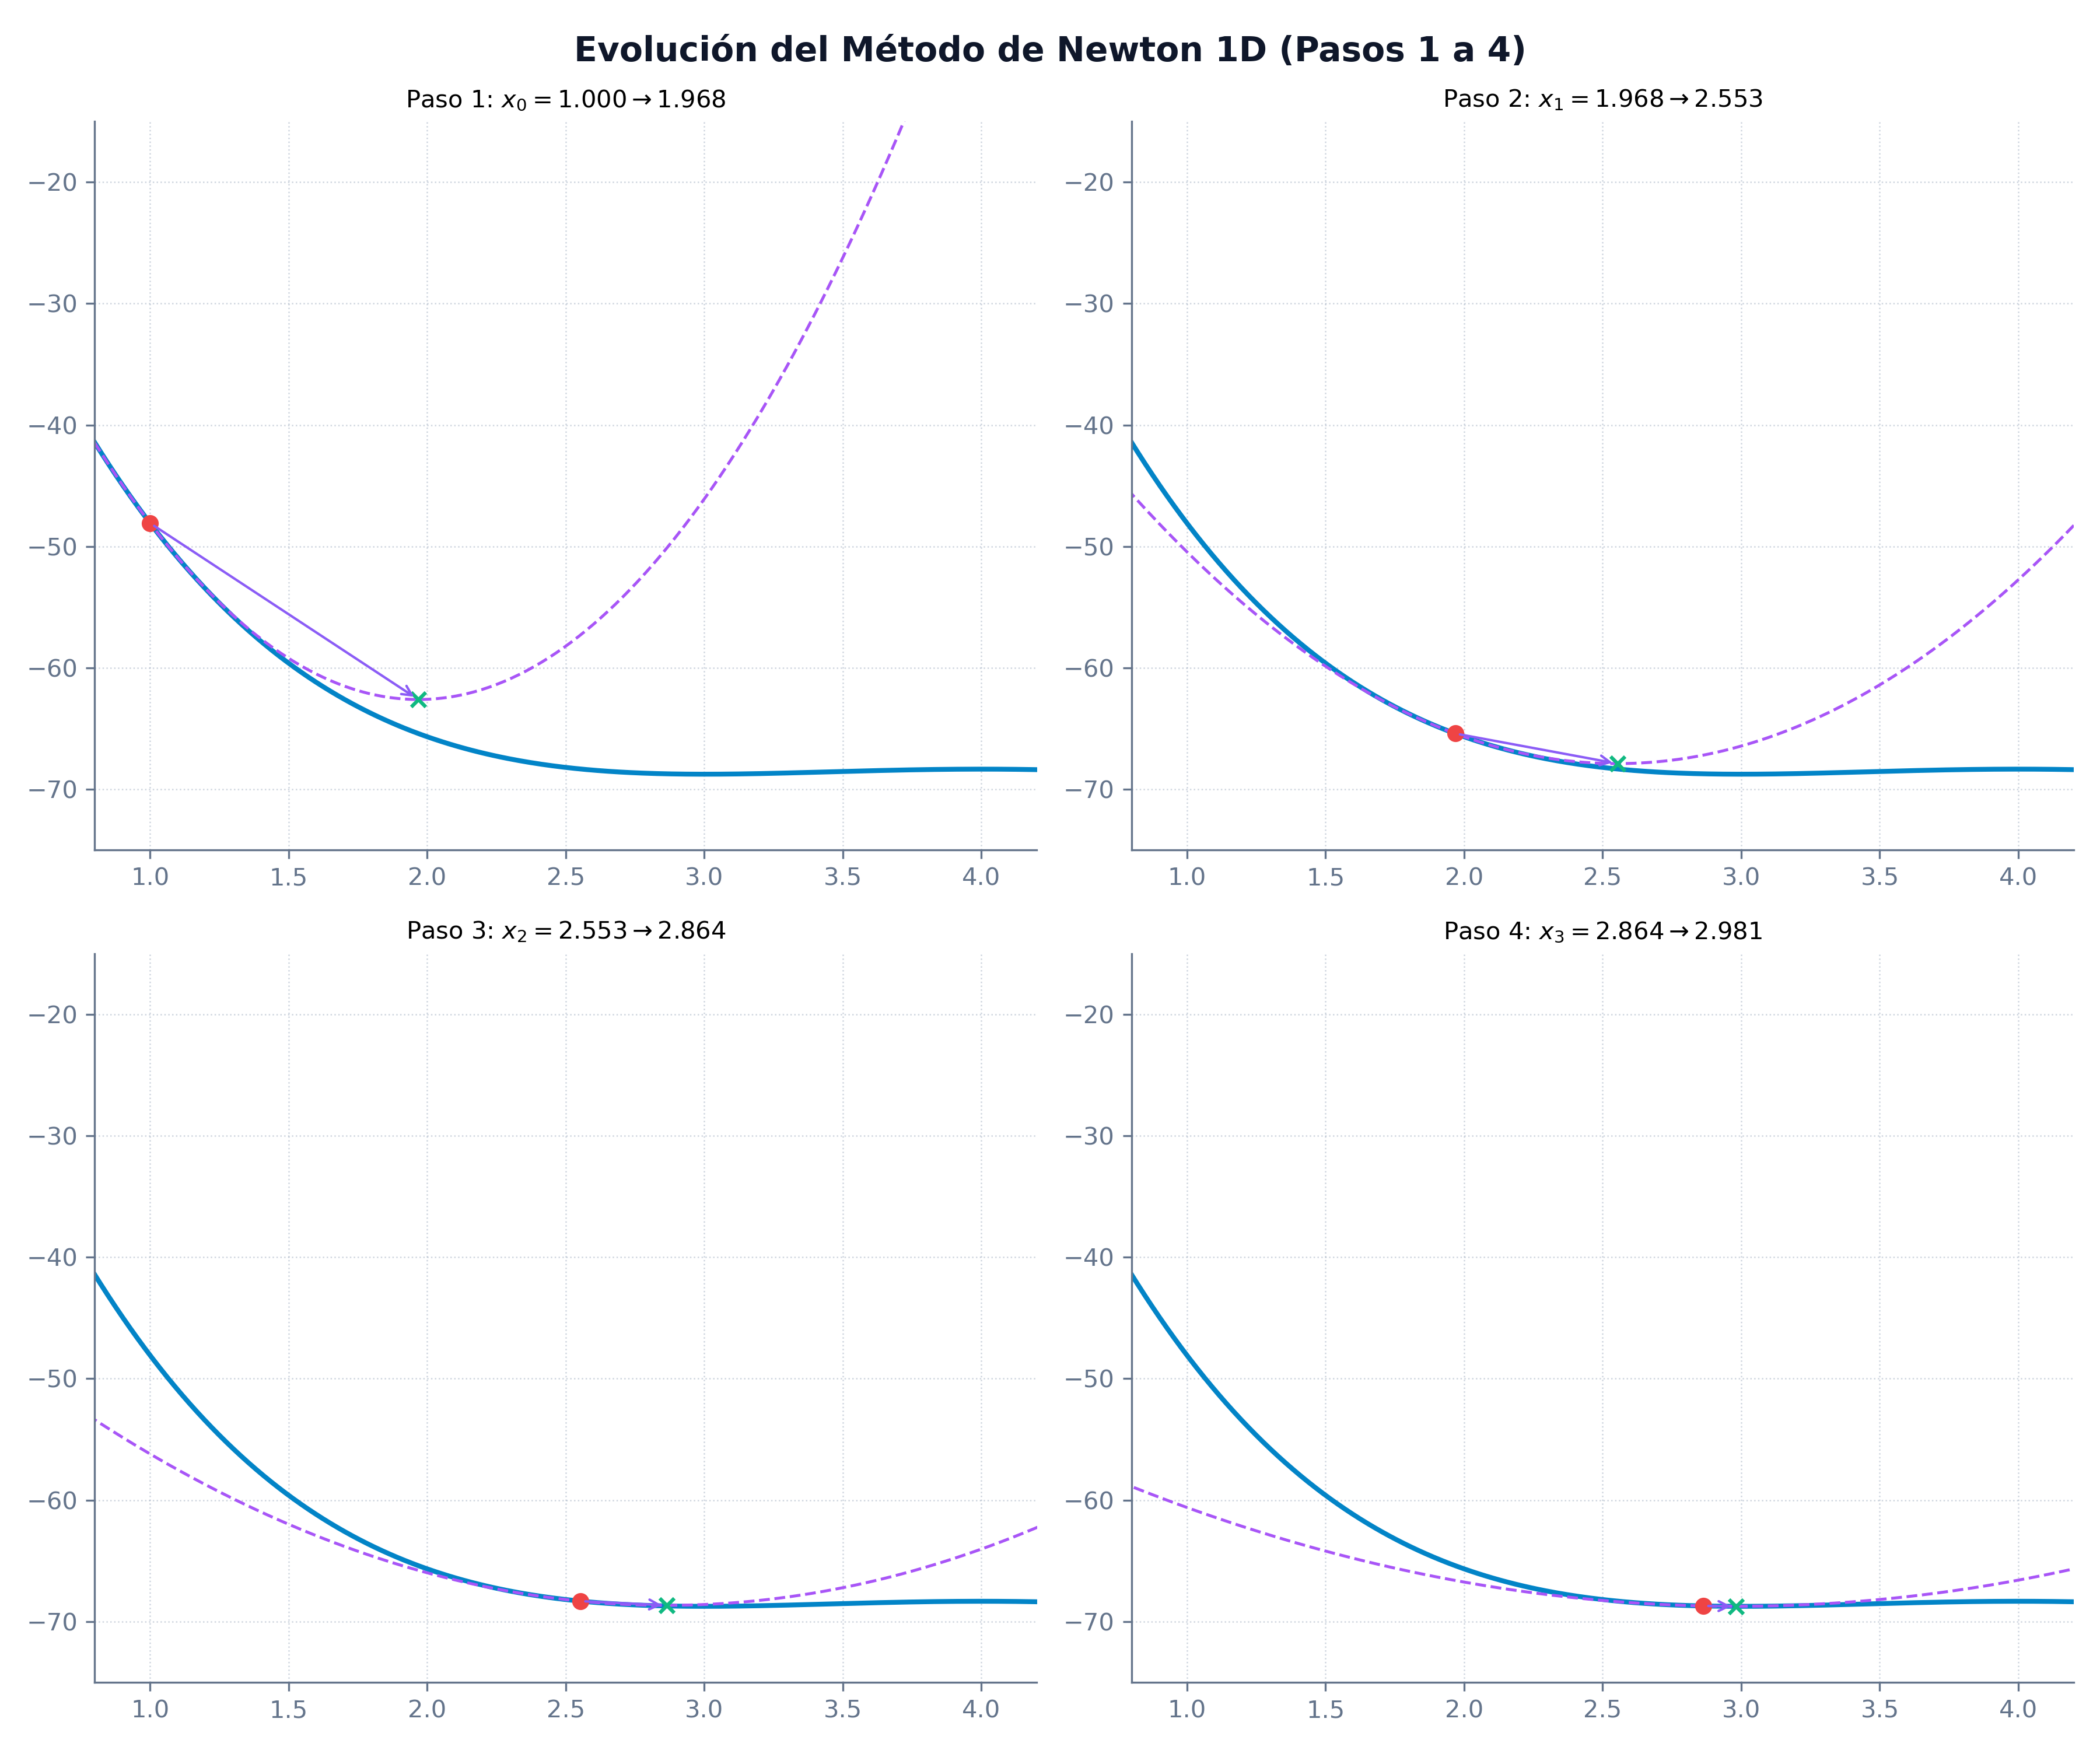
\includegraphics[width=0.85\linewidth,height=\textheight,keepaspectratio]{images/newton_1d_pasos.png}

}

\caption{\label{fig-newton-1d}Aproximaciones cuadráticas en el método de
Newton 1D (Pasos 1 a 4)}

\end{figure}%

\end{tcolorbox}

El \textbf{Método de la Secante} evita el inconveniente de calcular
analíticamente la segunda derivada \(f''(x)\) aproximándola
numéricamente por diferencias finitas a partir de las pendientes de los
dos últimos puntos evaluados:
\[f''(x_k) \approx \frac{f'(x_k) - f'(x_{k-1})}{x_k - x_{k-1}}\]
Sustituyendo esta aproximación en la fórmula de Newton, la regla
iterativa de la secante se calcula como:
\[x_{k+1} = x_k - f'(x_k) \cdot \frac{x_k - x_{k-1}}{f'(x_k) - f'(x_{k-1})}\]
Este método ofrece una convergencia superlineal de orden
\(\approx 1.618\) (la razón áurea) y requiere disponer de dos
estimaciones iniciales para iniciar las iteraciones (\(x_0\) y
\(x_{-1}\)).

\begin{tcolorbox}[enhanced jigsaw, toprule=.15mm, opacitybacktitle=0.6, coltitle=black, colbacktitle=quarto-callout-tip-color!10!white, title=\textcolor{quarto-callout-tip-color}{\faLightbulb}\hspace{0.5em}{Ejemplo: Método de la secante}, arc=.35mm, rightrule=.15mm, toptitle=1mm, breakable, bottomtitle=1mm, titlerule=0mm, colback=white, opacityback=0, leftrule=.75mm, colframe=quarto-callout-tip-color-frame, left=2mm, bottomrule=.15mm]

Minimizamos en el intervalo \([1, 4]\) la misma función partiendo de
\(x_{-1} = 1.0\) y \(x_0 = 1.5\). La derivada es
\(f'(x) = x^3 - 13x^2 + 54x - 72\).

\begin{itemize}
\tightlist
\item
  \textbf{Paso 1}: Puntos iniciales \(x_{-1} = 1.0\) y \(x_0 = 1.5\).

  \begin{itemize}
  \tightlist
  \item
    Evaluamos la derivada en ambos puntos:
    \[f'(1.0) = -30.0 \qquad f'(1.5) = -16.875\]
  \item
    Aplicamos la regla de la secante:
    \[x_1 = 1.5 - (-16.875) \cdot \frac{1.5 - 1.0}{-16.875 - (-30.0)} = 1.5 + 16.875 \cdot \frac{0.5}{13.125} \approx 2.1429\]
  \end{itemize}
\item
  \textbf{Paso 2}: Puntos \(x_0 = 1.5\) y \(x_1 = 2.1429\).

  \begin{itemize}
  \tightlist
  \item
    Evaluamos la derivada en el nuevo punto \(x_1\):
    \[f'(2.1429) \approx -6.1399\]
  \item
    Aplicamos la regla de la secante:
    \[x_2 = 2.1429 - (-6.1399) \cdot \frac{2.1429 - 1.5}{-6.1399 - (-16.875)} = 2.1429 + 6.1399 \cdot \frac{0.6429}{10.7351} \approx 2.5106\]
  \end{itemize}
\item
  \textbf{Pasos siguientes}: Aplicando iterativamente la secante
  obtenemos \(x_3 \approx 2.7707\), \(x_4 \approx 2.9157\),
  \(x_5 \approx 2.9807\), y finalmente
  \(x_7 \approx 2.9999 \approx 3.0\), convergiendo rápidamente al mínimo
  sin segundas derivadas.
\end{itemize}

\end{tcolorbox}

\section{Métodos multivariantes de optimización sin
restricciones}\label{muxe9todos-multivariantes-de-optimizaciuxf3n-sin-restricciones}

Para minimizar funciones multivariantes
\(f: \mathbb{R}^n \to \mathbb{R}\) sin restricciones, construimos una
sucesión iterativa a partir de una dirección de búsqueda \(d_k\) y un
tamaño de paso \(\alpha_k > 0\): \[x_{k+1} = x_k + \alpha_k d_k\] Para
garantizar que el algoritmo avance reduciendo la función en cada paso,
la dirección \(d_k\) debe ser de descenso, lo que exige matemáticamente
que forme un ángulo obtuso con el gradiente de la función en el punto
actual: \[\nabla f(x_k)^T d_k < 0\]

Para ilustrar el funcionamiento de los algoritmos multivariantes,
utilizaremos a lo largo del capítulo dos funciones de prueba
representativas en \(\mathbb{R}^2\):

\begin{enumerate}
\def\labelenumi{\arabic{enumi}.}
\tightlist
\item
  \textbf{Función de distancia circular (desacoplada)}:
  \[f(x, y) = (x-2)^2 + (y-1)^2\] Su forma geométrica es la de un cuenco
  circular (paraboloide de revolución) con curvas de nivel perfectamente
  redondas, lo que facilita el comportamiento de los métodos por no
  existir acoplamiento cruzado (ver Figura~\ref{fig-funciones-3d-1}).
\item
  \textbf{Función cuadrática mal acondicionada (acoplada)}:
  \[f(x, y) = 8x^2 + 3xy + 7y^2 - 25x + 31y - 29\] Presenta curvas de
  nivel elípticas muy alargadas y un término cruzado \(3xy\) que acopla
  las variables, simulando un problema de optimización realista de
  curvatura desigual (ver Figura~\ref{fig-funciones-3d-2}).
\end{enumerate}

\begin{figure}

\begin{minipage}{0.50\linewidth}

\centering{

\pandocbounded{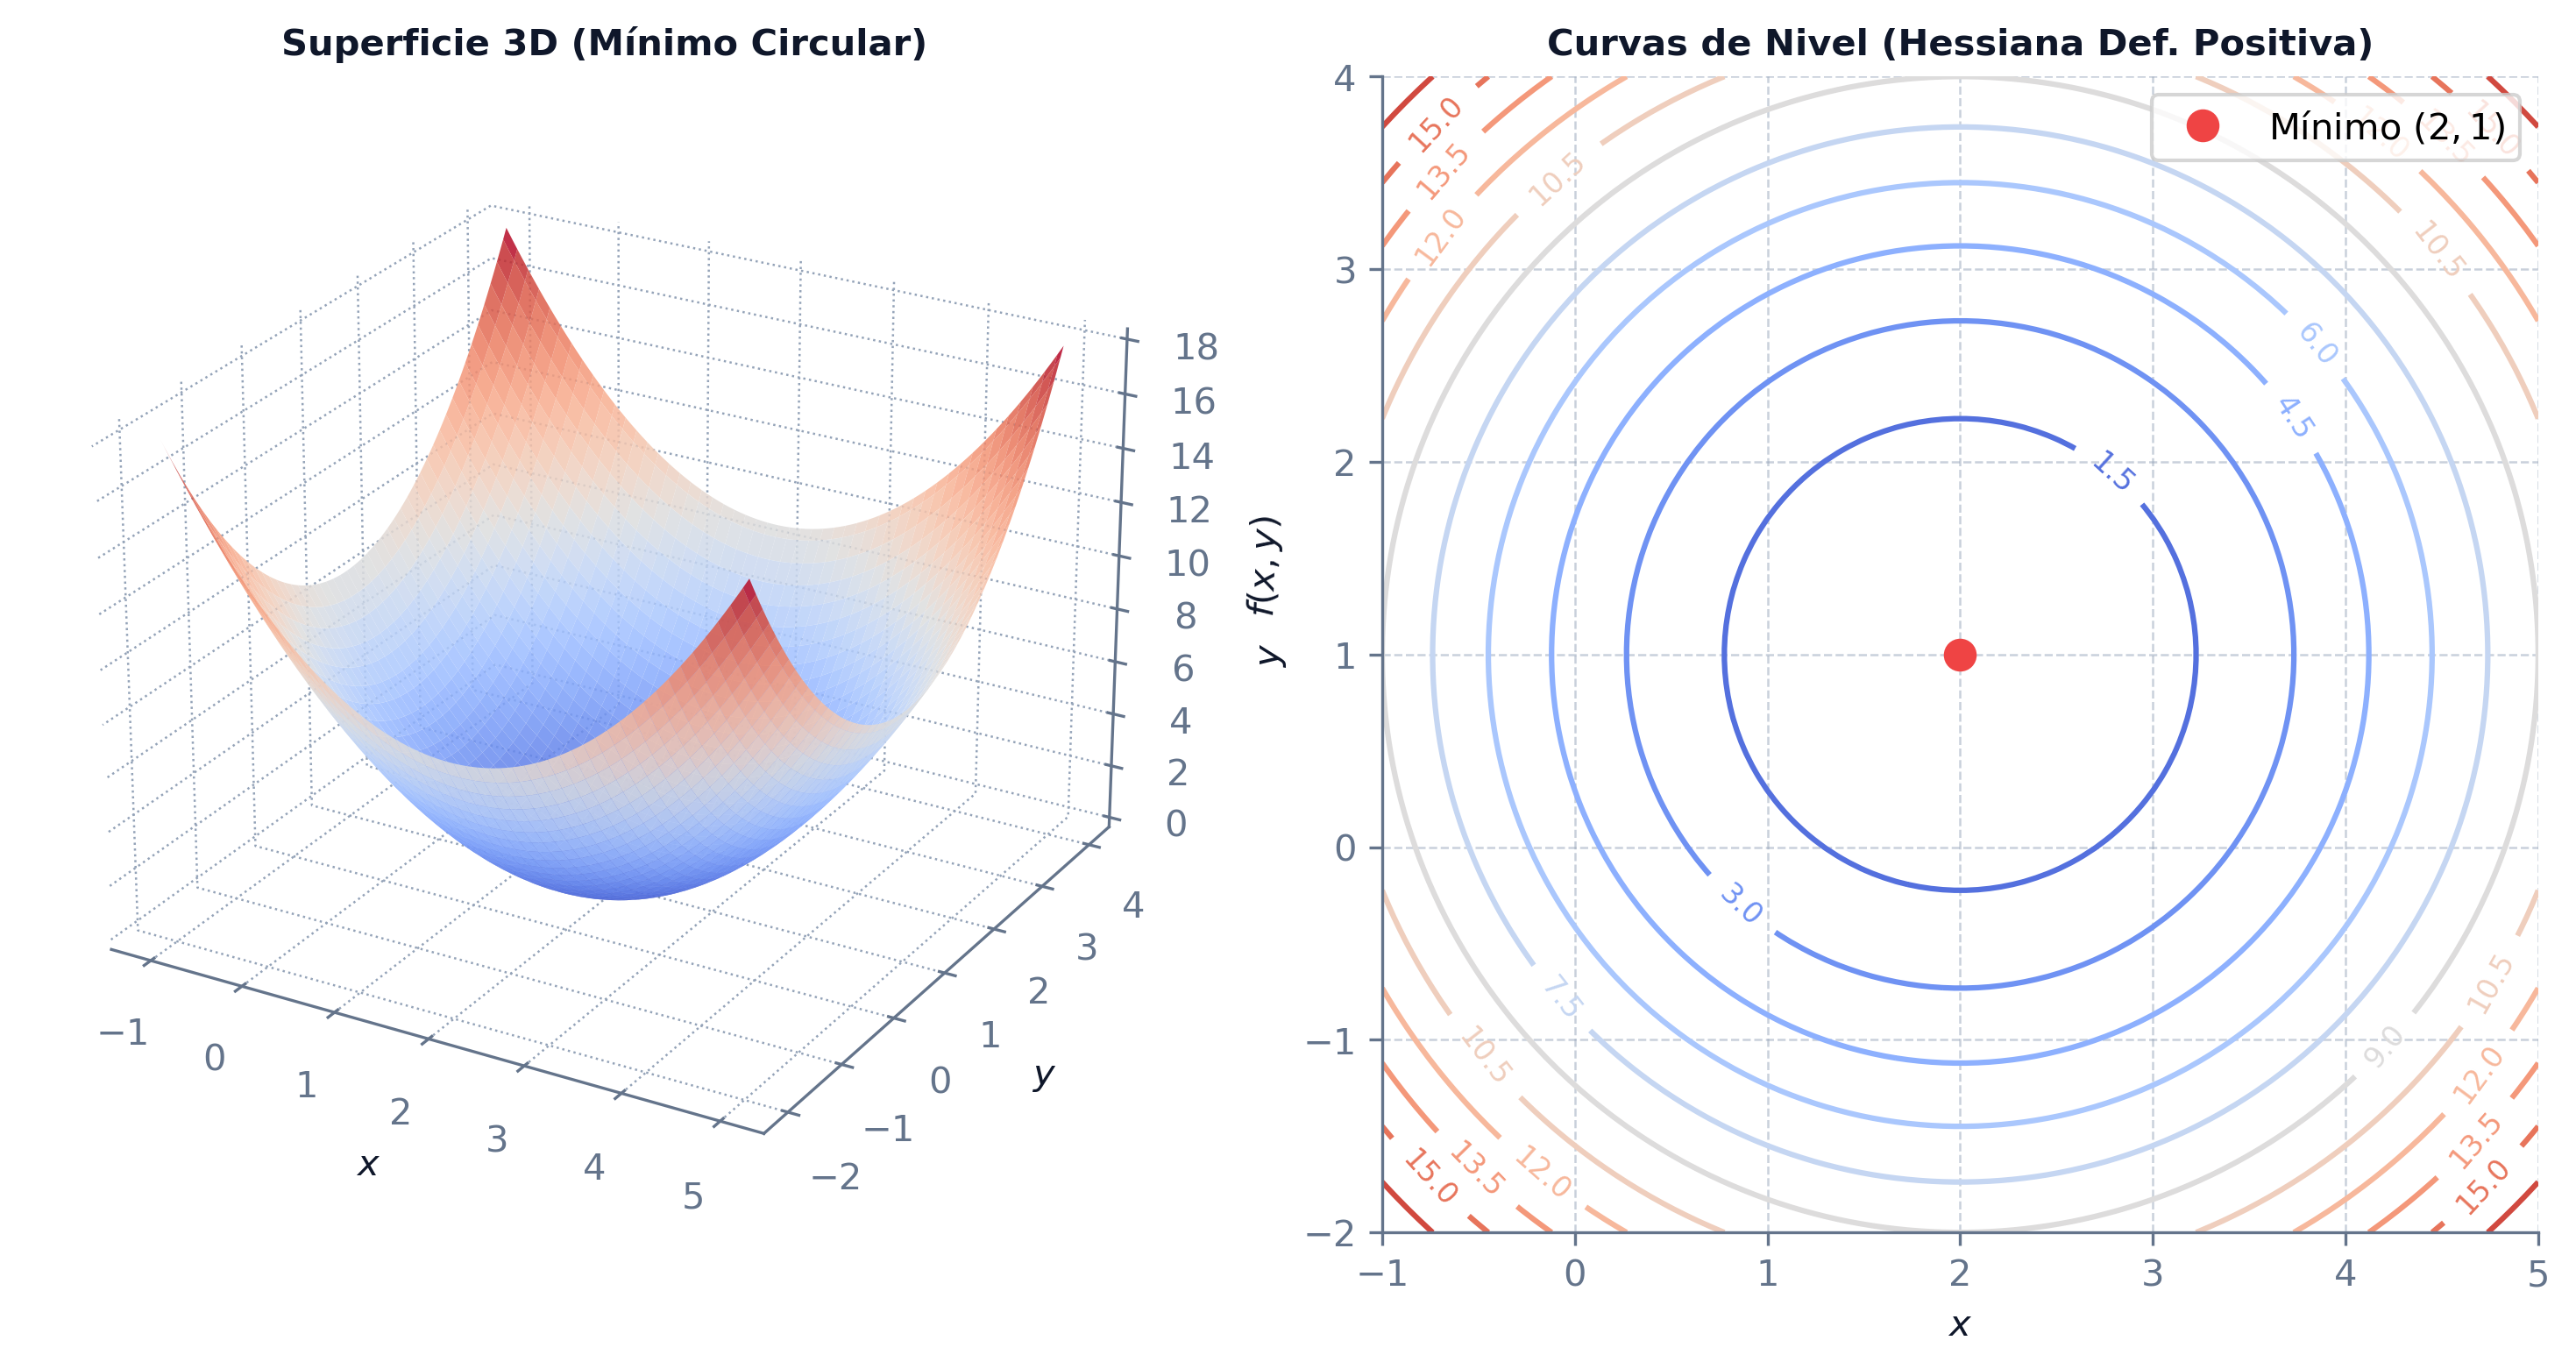
\includegraphics[keepaspectratio]{images/funcion_distancia_3d.png}}

}

\subcaption{\label{fig-funciones-3d-1}Superficie 3D de la función de
distancia circular desacoplada}

\end{minipage}%
%
\begin{minipage}{0.50\linewidth}

\centering{

\pandocbounded{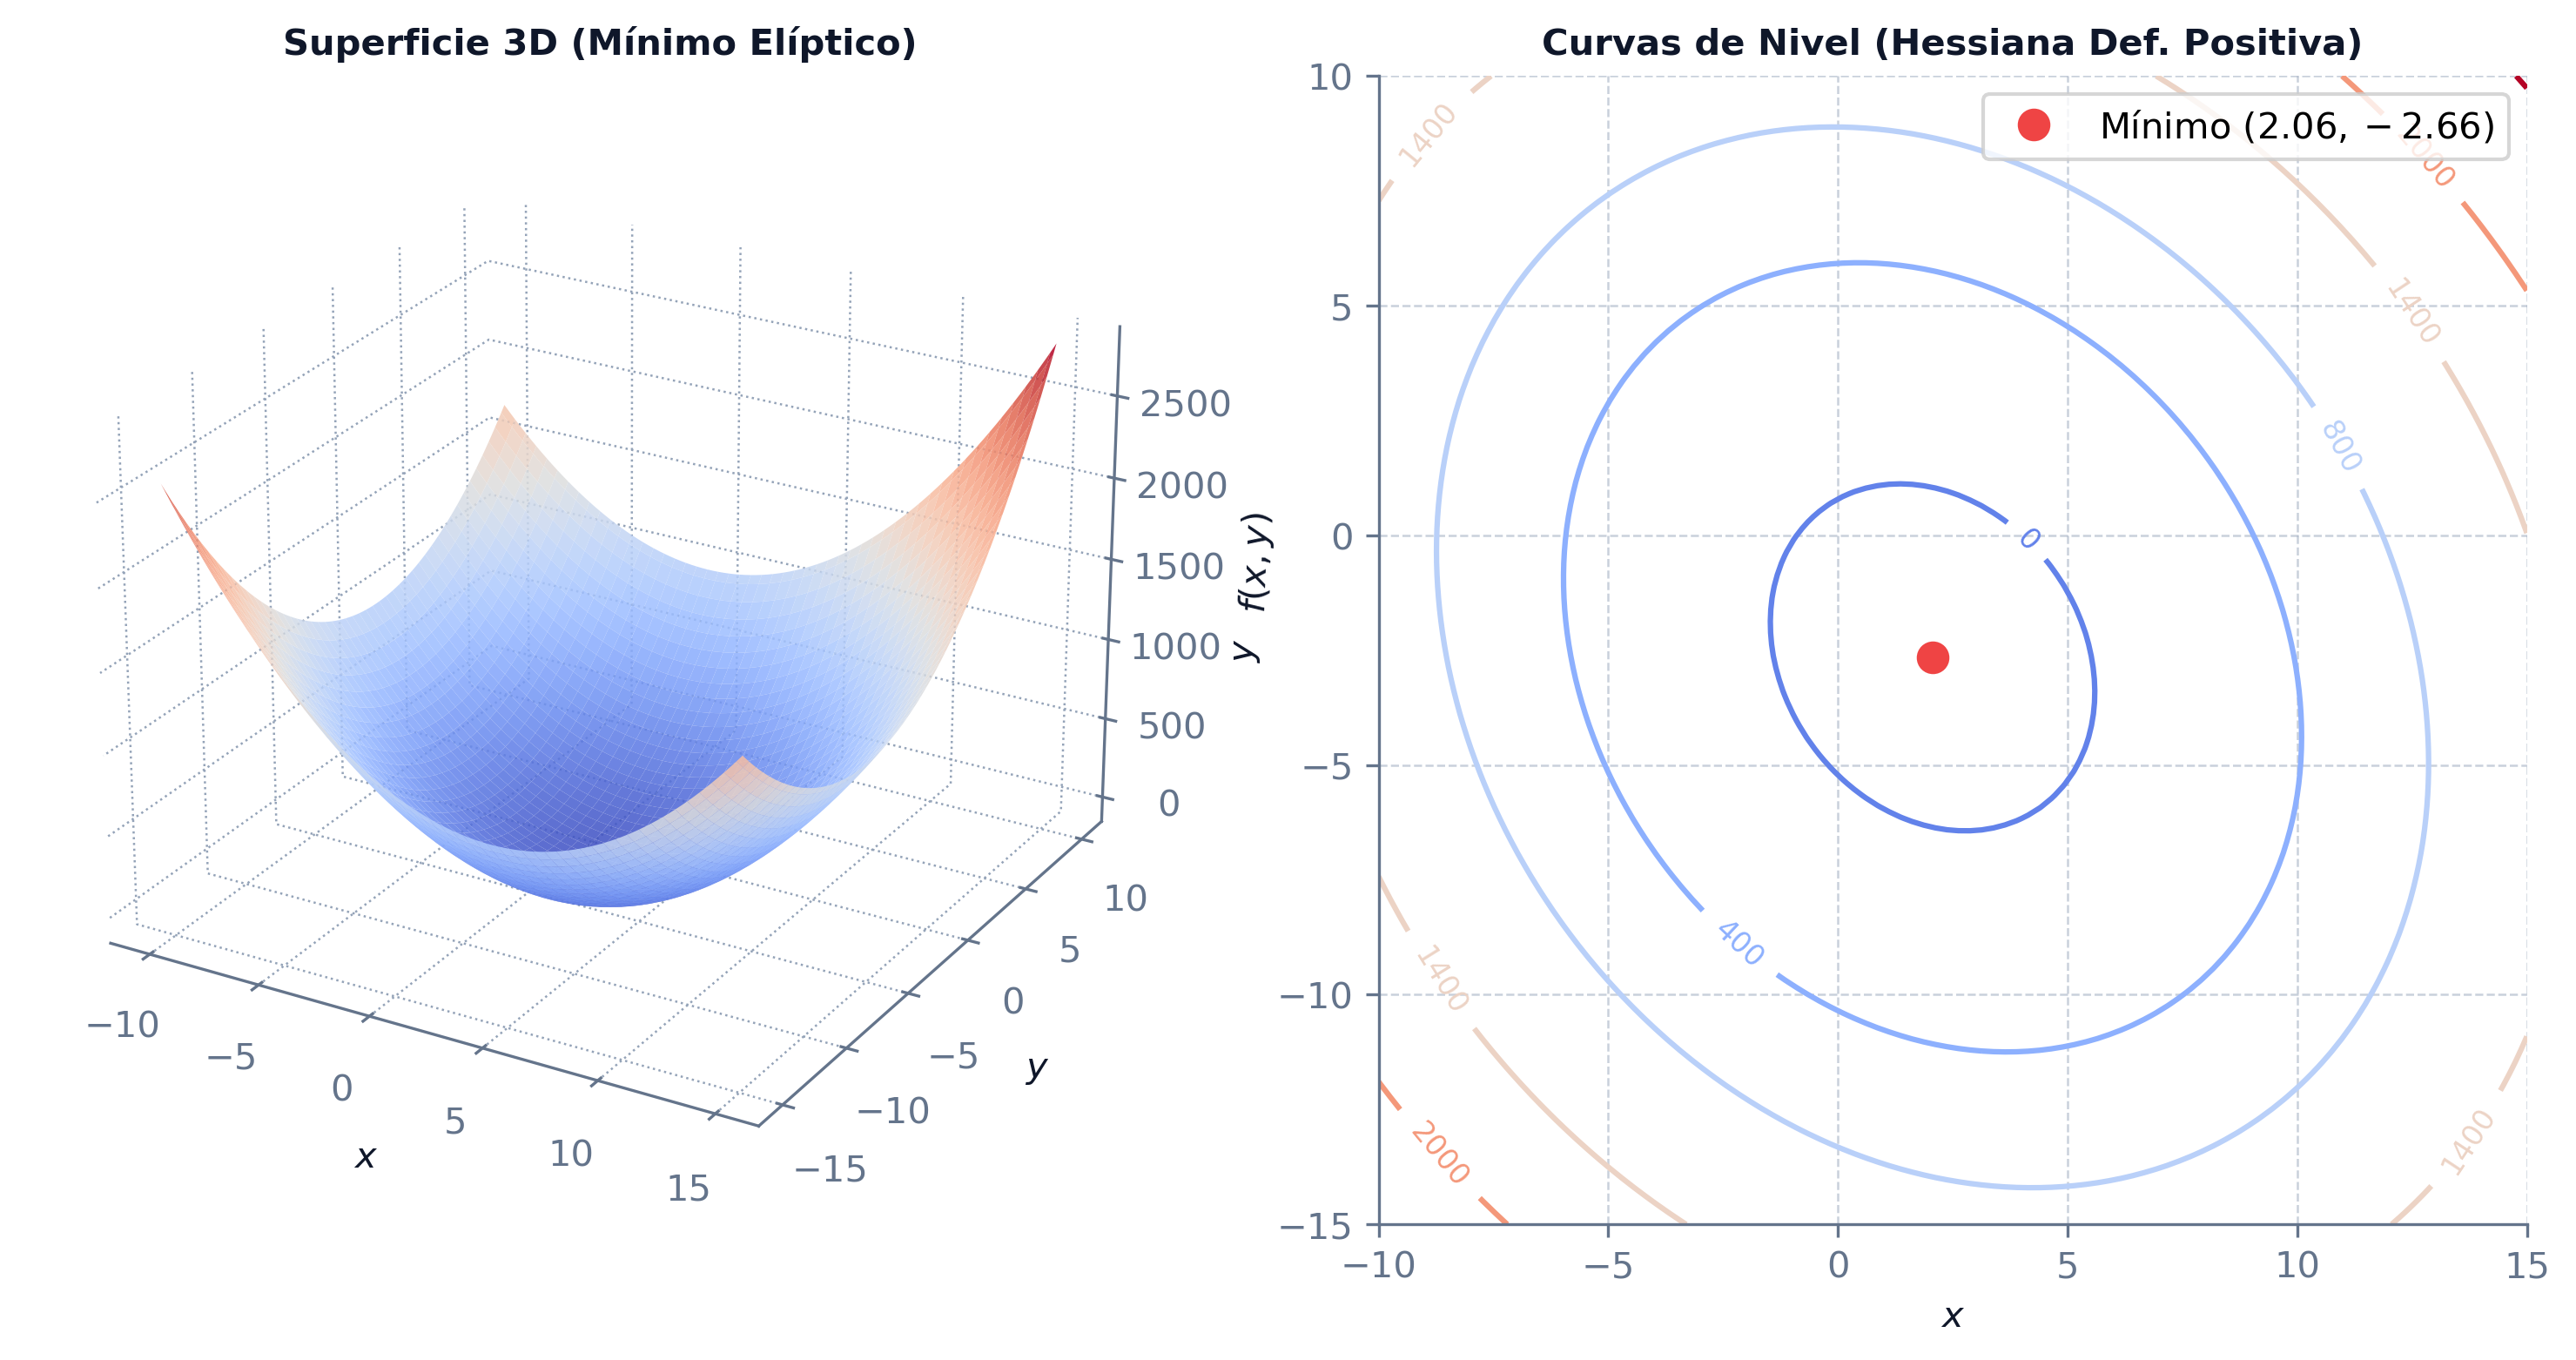
\includegraphics[keepaspectratio]{images/funcion_cuadratica_3d.png}}

}

\subcaption{\label{fig-funciones-3d-2}Superficie 3D de la función
cuadrática acoplada}

\end{minipage}%

\caption{\label{fig-funciones-3d}Superficies tridimensionales de las
funciones de prueba en varias variables}

\end{figure}%

\subsection{Método de las coordenadas
cíclicas}\label{muxe9todo-de-las-coordenadas-cuxedclicas}

El \textbf{método de las coordenadas cíclicas} (o \emph{coordinate
descent}) es uno de los algoritmos de optimización multivariante más
elementales e intuitivos. Su principal ventaja radica en que
\textbf{evita por completo el cálculo de gradientes y matrices
hessianas}, aplicando una estrategia de descomposición: en lugar de
buscar la dirección óptima en el espacio multidimensional
\(\mathbb{R}^n\), descompone el problema en una sucesión ordenada de
búsquedas unidimensionales a lo largo de los ejes coordenados.

El procedimiento explora de forma secuencial cada una de las variables
de decisión, manteniendo fijas las restantes \(n-1\). Las direcciones de
búsqueda coinciden cíclicamente con los vectores de la base canónica de
\(\mathbb{R}^n\), definidos formalmente como
\(d_k = e_{(k \bmod n) + 1}\), donde \(e_i\) es el \(i\)-ésimo vector
unitario con un 1 en la posición \(i\) y ceros en las demás. El proceso
se articula en tres etapas fundamentales:

\begin{enumerate}
\def\labelenumi{\arabic{enumi}.}
\item
  \textbf{Paso unidimensional}: Estando en el punto iterado \(x^{(k)}\),
  se selecciona el eje coordenado correspondiente y se resuelve un
  subproblema de optimización unidimensional restringido a esa única
  coordenada:
  \[ \min_{\alpha \in \mathbb{R}} \quad \phi(\alpha) = f(x^{(k)} + \alpha e_i) \]
  Esta minimización escalar se resuelve de forma analítica igualando la
  derivada a cero si la función es elemental, o bien mediante los
  algoritmos de búsqueda unidimensional vistos anteriormente (como la
  Sección Áurea). Una vez obtenido el paso óptimo \(\alpha^*\), el punto
  se actualiza como \(x^{(k+1)} = x^{(k)} + \alpha^* e_i\).
\item
  \textbf{Cierre de ciclo}: El procedimiento se repite variando
  sucesivamente la variable 1, luego la variable 2, y así sucesivamente
  hasta completar la variable \(n\). A la realización sucesiva de estas
  \(n\) búsquedas unidimensionales ortogonales se le denomina \textbf{un
  ciclo}.
\item
  \textbf{Criterio de convergencia}: Tras completar un ciclo entero por
  todas las variables, se comprueba si el desplazamiento acumulado entre
  el punto inicial y el punto final del ciclo es inferior a una
  tolerancia prefijada:
  \[ \| x^{(k+n)} - x^{(k)} \| \le \epsilon \quad \text{o bien} \quad |f(x^{(k+n)}) - f(x^{(k)})| \le \epsilon \]
  Si se verifica la condición de parada, el algoritmo finaliza con
  éxito. En caso contrario, se inicia un nuevo ciclo comenzando
  nuevamente por la primera coordenada.
\end{enumerate}

El rendimiento y velocidad de convergencia de este método depende
críticamente de la estructura geométrica de la función y del
acoplamiento entre sus variables:

\begin{itemize}
\tightlist
\item
  \textbf{Variables desacopladas}: Si la función no contiene términos de
  interacción cruzada entre variables y su matriz hessiana es diagonal,
  las curvas de nivel son circunferencias o elipses cuyos ejes
  principales son paralelos a los ejes coordenados. En este escenario
  ideal, el algoritmo alcanza el mínimo global exacto en un único ciclo
  de \(n\) pasos ortogonales.
\item
  \textbf{Variables acopladas}: Cuando existen términos cruzados (como
  un término bilineal \(x_i x_j\)), las curvas de nivel elípticas
  aparecen rotadas respecto a los ejes canónicos. Como el algoritmo solo
  puede desplazarse en giros ortogonales de 90 grados paralelos a los
  ejes, se ve obligado a avanzar trazando una \textbf{trayectoria en
  escalera o zigzag}, requiriendo una gran cantidad de ciclos y pasos
  progresivamente más cortos para aproximarse al óptimo.
\end{itemize}

\begin{tcolorbox}[enhanced jigsaw, toprule=.15mm, opacitybacktitle=0.6, coltitle=black, colbacktitle=quarto-callout-tip-color!10!white, title=\textcolor{quarto-callout-tip-color}{\faLightbulb}\hspace{0.5em}{Ejemplo: Coordenadas cíclicas}, arc=.35mm, rightrule=.15mm, toptitle=1mm, breakable, bottomtitle=1mm, titlerule=0mm, colback=white, opacityback=0, leftrule=.75mm, colframe=quarto-callout-tip-color-frame, left=2mm, bottomrule=.15mm]

\begin{itemize}
\item
  \textbf{Variables Desacopladas}: Minimizamos la función de distancia
  \(f(x, y) = (x-2)^2 + (y-1)^2\) (ver
  Figura~\ref{fig-coord-ciclicas-1}) partiendo de \(x_0 = (0, 0)^T\).

  \begin{itemize}
  \tightlist
  \item
    \emph{Paso 1}: Minimizamos respecto a \(x\):
    \[ \min_{x} \quad f(x, 0) = (x-2)^2 + 1 \implies x_1 = (2, 0)^T \]
  \item
    \emph{Paso 2}: Minimizamos respecto a \(y\):
    \[ \min_{y} \quad f(2, y) = (y-1)^2 \implies x_2 = (2, 1)^T \]
  \end{itemize}

  Al no existir términos de acoplamiento cruzado entre las variables (la
  matriz hessiana es diagonal), el algoritmo localiza el mínimo exacto
  en una única iteración de \(n=2\) pasos ortogonales.
\end{itemize}

\begin{figure}[H]

\centering{

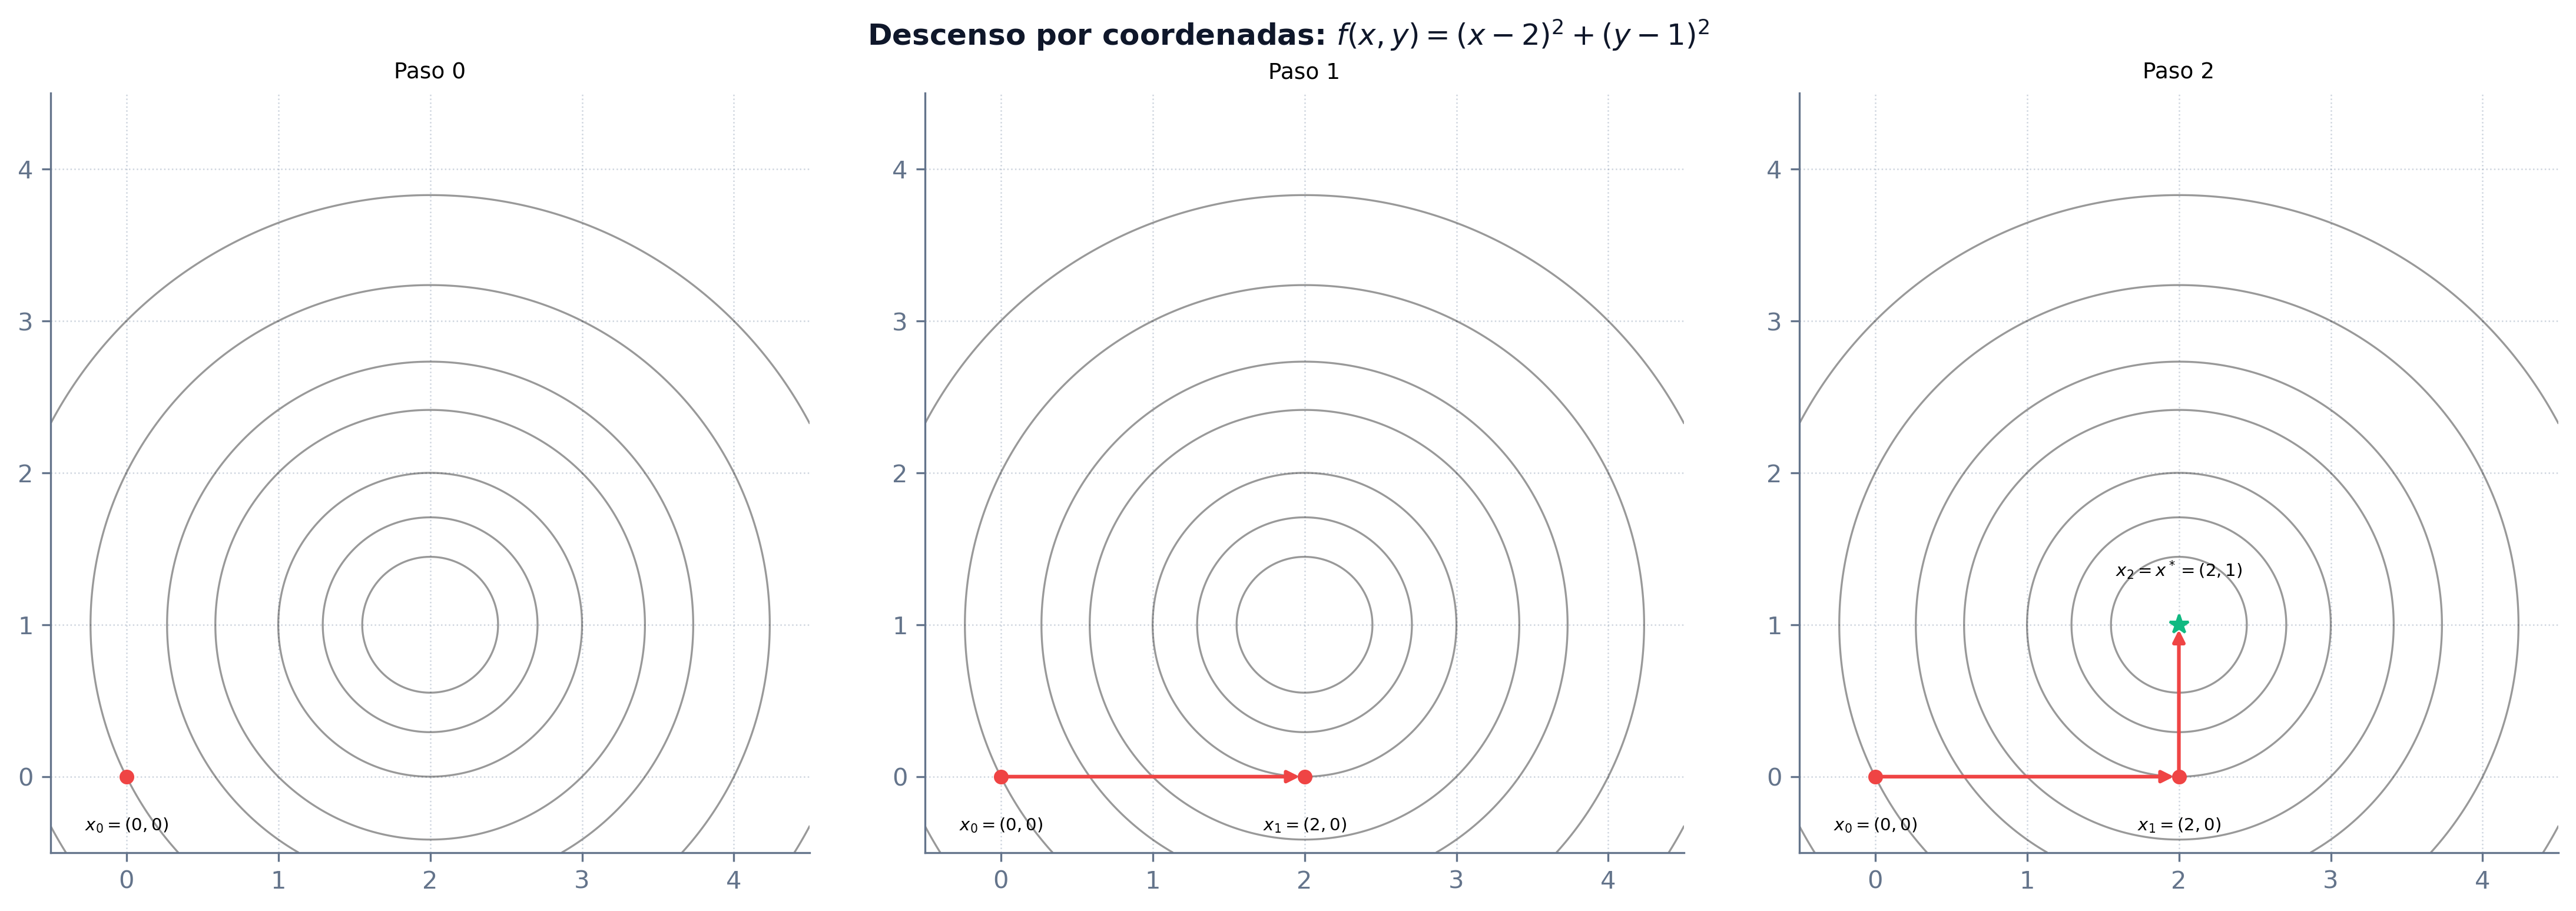
\includegraphics[width=1\linewidth,height=\textheight,keepaspectratio]{images/coordenadas_ciclicas_ej1_pasos.png}

}

\caption{\label{fig-coord-ciclicas-1}Descenso por coordenadas cíclicas:
secuencia de pasos sobre curvas de nivel circulares}

\end{figure}%

\begin{itemize}
\item
  \textbf{Variables Acopladas}: Minimizamos
  \(f(x, y) = 8x^2 + 3xy + 7y^2 - 25x + 31y - 29\) (ver
  Figura~\ref{fig-coord-ciclicas-2}) partiendo de \(x_0 = (0, 0)^T\).

  \begin{itemize}
  \tightlist
  \item
    \emph{Paso 1}: Minimizamos respecto a \(x\):
    \[ \min_{x} \quad f(x, 0) = 8x^2 - 25x - 29 \implies 16x - 25 = 0 \implies x_1 = (1.5625, 0)^T \]
  \item
    \emph{Paso 2}: Minimizamos respecto a \(y\) manteniendo
    \(x = 1.5625\):
    \[ \min_{y} \quad f(1.5625, y) = 7y^2 + 35.6875y + \text{ct} \implies 14y + 35.6875 = 0 \implies \]
    \[y = -\frac{571}{224} \approx -2.5491 \] Lo que resulta en el punto
    \(x_2 = (1.5625, -2.5491)^T\).
  \item
    \emph{Paso 3}: Minimizamos de nuevo respecto a \(x\) con
    \(y = -2.5491\):
    \[ \min_{x} \quad f(x, -2.5491) = 8x^2 - 32.6473x + \text{ct} \implies 16x - 32.6473 = 0 \implies\]
    \[x_3 = (2.0405, -2.5491)^T \]
  \end{itemize}

  Debido al acoplamiento bilineal inducido por el término \(3xy\), la
  trayectoria dibuja un patrón de ``escalera'', requiriendo múltiples
  ciclos para aproximarse al mínimo global situado en
  \(x^* = (2.060, -2.656)\).
\end{itemize}

\begin{figure}[H]

\centering{

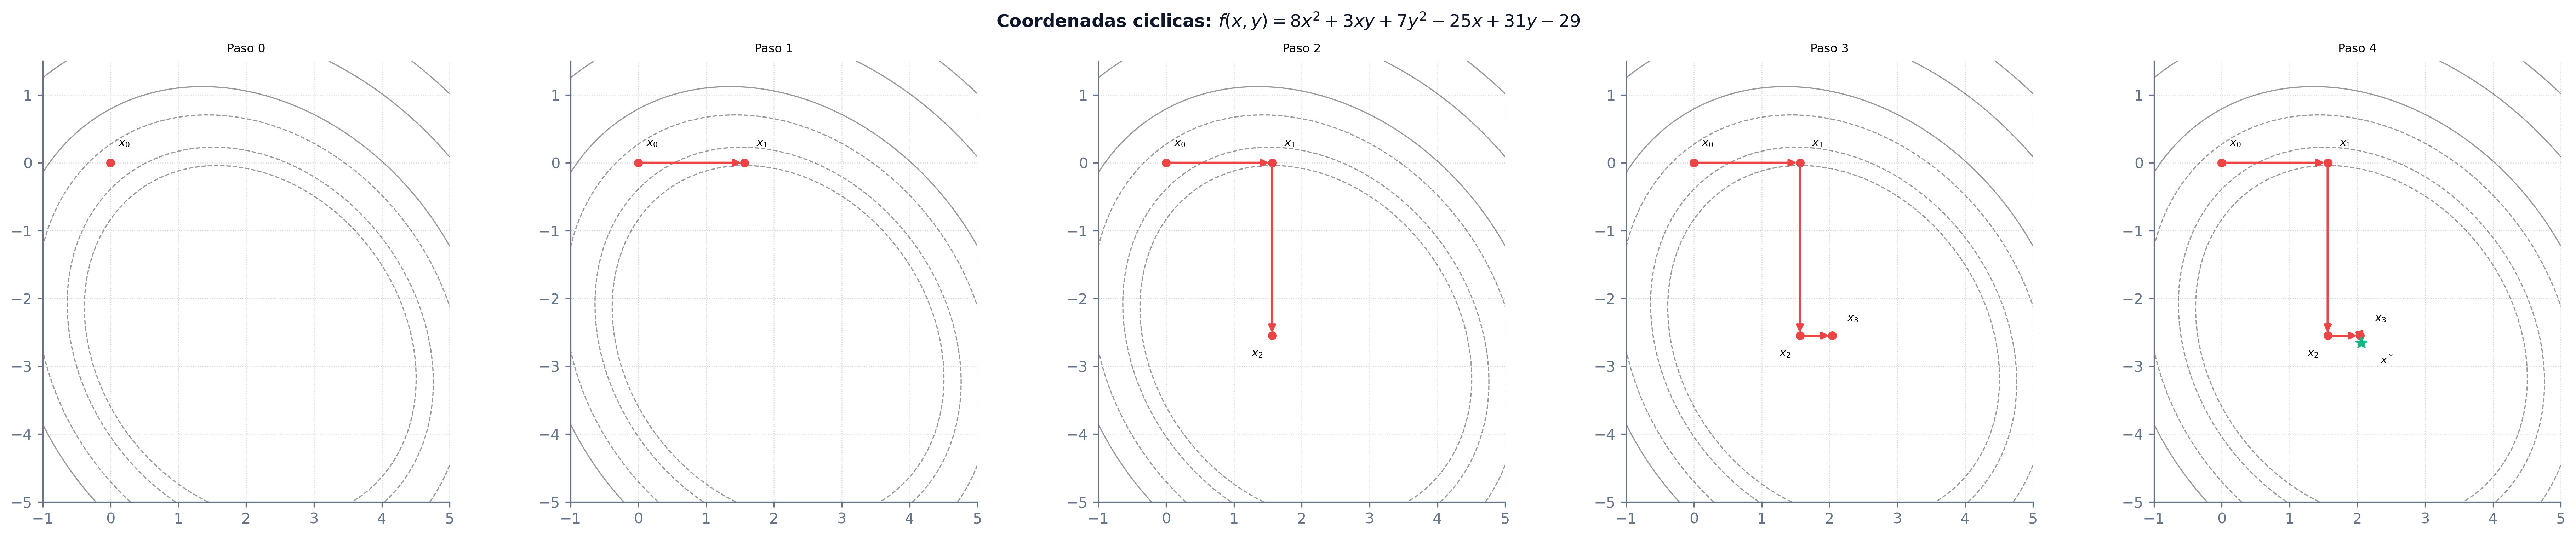
\includegraphics[width=1\linewidth,height=\textheight,keepaspectratio]{images/coordenadas_ciclicas_ej2_pasos.png}

}

\caption{\label{fig-coord-ciclicas-2}Trayectoria en escalera del
descenso por coordenadas cíclicas sobre una función cuadrática acoplada}

\end{figure}%

\end{tcolorbox}

\subsection{Método del máximo
descenso}\label{muxe9todo-del-muxe1ximo-descenso}

El \textbf{método del máximo descenso} (o \emph{steepest descent} /
gradiente descendente) es el algoritmo iterativo de primer orden
fundamental en optimización continua. La dirección de búsqueda se define
como aquella en la que la función objetivo decrece de manera más rápida
a nivel local, dada por el opuesto del vector gradiente:
\[d_k = -\nabla f(x_k)\] A partir del punto actual \(x_k\), la
actualización se realiza según la expresión
\(x_{k+1} = x_k + \alpha_k d_k\), donde \(\alpha_k > 0\) representa la
longitud del paso. En el esquema teórico de \textbf{búsqueda de línea
exacta}, el tamaño de paso óptimo se determina minimizando la función
unidimensional a lo largo del rayo de descenso:
\[\alpha_k = \arg\min_{\alpha > 0} f(x_k - \alpha \nabla f(x_k))\] En
aplicaciones computacionales complejas donde evaluar la función de forma
exhaustiva resulta prohibitivo, suele recurrirse a esquemas de
\textbf{búsqueda de línea inexacta} (como las condiciones de Armijo o
Wolfe), que garantizan una disminución suficiente del valor de la
función sin exigir la localización exacta del mínimo unidimensional.

El algoritmo itera sucesivamente calculando la dirección opuesta al
gradiente y actualizando el punto hasta satisfacer alguno de los
siguientes \textbf{criterios de parada}:

\begin{itemize}
\tightlist
\item
  \textbf{Estacionariedad}: La norma del vector gradiente es inferior a
  una tolerancia prefijada, \(\|\nabla f(x_k)\| \le \epsilon_g\), lo que
  garantiza que nos encontramos en las proximidades de un punto crítico.
\item
  \textbf{Estancamiento del paso}: El desplazamiento relativo o absoluto
  entre dos iteraciones consecutivas es despreciable,
  \(\|x_{k+1} - x_k\| \le \epsilon_x\).
\item
  \textbf{Estancamiento de la función objetivo}: La reducción en el
  valor de la función objetivo cae por debajo del umbral mínimo,
  \(|f(x_{k+1}) - f(x_k)| \le \epsilon_f\).
\item
  \textbf{Límite computacional}: Se alcanza un número máximo prefijado
  de iteraciones \(k \ge K_{\max}\).
\end{itemize}

Una propiedad matemática de la búsqueda lineal exacta en el método de
máximo descenso es que las direcciones de búsqueda en iteraciones
consecutivas son estrictamente ortogonales entre sí:
\[d_k^T d_{k+1} = 0\]

Para demostrarlo, definimos la función unidimensional
\(\phi(\alpha) = f(x_k + \alpha d_k)\) que se minimiza para hallar
\(\alpha_k\). La condición de óptimo exige que su derivada con respecto
al tamaño de paso sea nula en \(\alpha_k\):
\[\phi'(\alpha_k) = \nabla f(x_k + \alpha_k d_k)^T d_k = 0\] Dado que el
nuevo punto es \(x_{k+1} = x_k + \alpha_k d_k\), se tiene que
\(\nabla f(x_{k+1})^T d_k = 0\). Puesto que las direcciones consecutivas
son proporcionales a los gradientes (\(d_{k+1} = -\nabla f(x_{k+1})\) y
\(d_k = -\nabla f(x_k)\)), se concluye de forma directa la
ortogonalidad: \[d_{k+1}^T d_k = 0\]

Esta ortogonalidad geométrica provoca que, si la función presenta curvas
de nivel elípticas muy alargadas (lo que ocurre cuando la matriz
hessiana está mal condicionada y existe una gran disparidad entre su
autovalor máximo y mínimo, \(\lambda_{\max} \gg \lambda_{\min}\)), el
algoritmo realice continuos giros de 90 grados, generando un patrón en
\textbf{zigzag} que ralentiza sustancialmente la velocidad de
convergencia hacia el óptimo, tal y como se observa en la
Figura~\ref{fig-steepest-descent}.

\begin{tcolorbox}[enhanced jigsaw, toprule=.15mm, opacitybacktitle=0.6, coltitle=black, colbacktitle=quarto-callout-tip-color!10!white, title=\textcolor{quarto-callout-tip-color}{\faLightbulb}\hspace{0.5em}{Ejemplo: Máximo descenso}, arc=.35mm, rightrule=.15mm, toptitle=1mm, breakable, bottomtitle=1mm, titlerule=0mm, colback=white, opacityback=0, leftrule=.75mm, colframe=quarto-callout-tip-color-frame, left=2mm, bottomrule=.15mm]

Minimizamos \(f(x, y) = 8x^2 + 3xy + 7y^2 - 25x + 31y - 29\) partiendo
de \(x_0 = (0, 0)^T\).

\begin{itemize}
\item
  \textbf{Gradiente en \(x_0\)}: Calculamos el gradiente de la función y
  lo evaluamos en el origen:
  \[ \nabla f(x_0) = \begin{pmatrix} 16x + 3y - 25 \\ 3x + 14y + 31 \end{pmatrix}_{x=(0,0)} = \begin{pmatrix} -25 \\ 31 \end{pmatrix} \]
  La dirección de descenso óptima es el gradiente negativo:
  \[ d_0 = -\nabla f(x_0) = \begin{pmatrix} 25 \\ -31 \end{pmatrix} \]
\item
  \textbf{Búsqueda de línea exacta}: Minimizamos la función respecto al
  tamaño del paso \(\alpha\):
  \[ \phi(\alpha) = f(x_0 + \alpha d_0) = f(25\alpha, -31\alpha) = 9402\alpha^2 - 1586\alpha - 29 \]
  Derivando e igualando a cero:
  \[ \phi'(\alpha) = 18804\alpha - 1586 = 0 \implies \alpha_0 = \frac{1586}{18804} \approx 0.0843 \]
\item
  \textbf{Actualización del punto}: El nuevo punto en la primera
  iteración es:
  \[ x_1 = x_0 + \alpha_0 d_0 = \begin{pmatrix} 0 \\ 0 \end{pmatrix} + 0.0843 \begin{pmatrix} 25 \\ -31 \end{pmatrix} = \begin{pmatrix} 2.109 \\ -2.615 \end{pmatrix} \]
  El nuevo gradiente en \(x_1\) es:
  \[ \nabla f(x_1) \approx \begin{pmatrix} 0.8925 \\ 0.7225 \end{pmatrix} \]
  Verificamos la ortogonalidad respecto a la dirección de búsqueda
  anterior:
  \[ d_0^T \nabla f(x_1) = 25(0.8925) - 31(0.7225) \approx 0 \] Lo cual
  ilustra la ortogonalidad requerida por la búsqueda exacta.
\end{itemize}

\begin{figure}[H]

\centering{

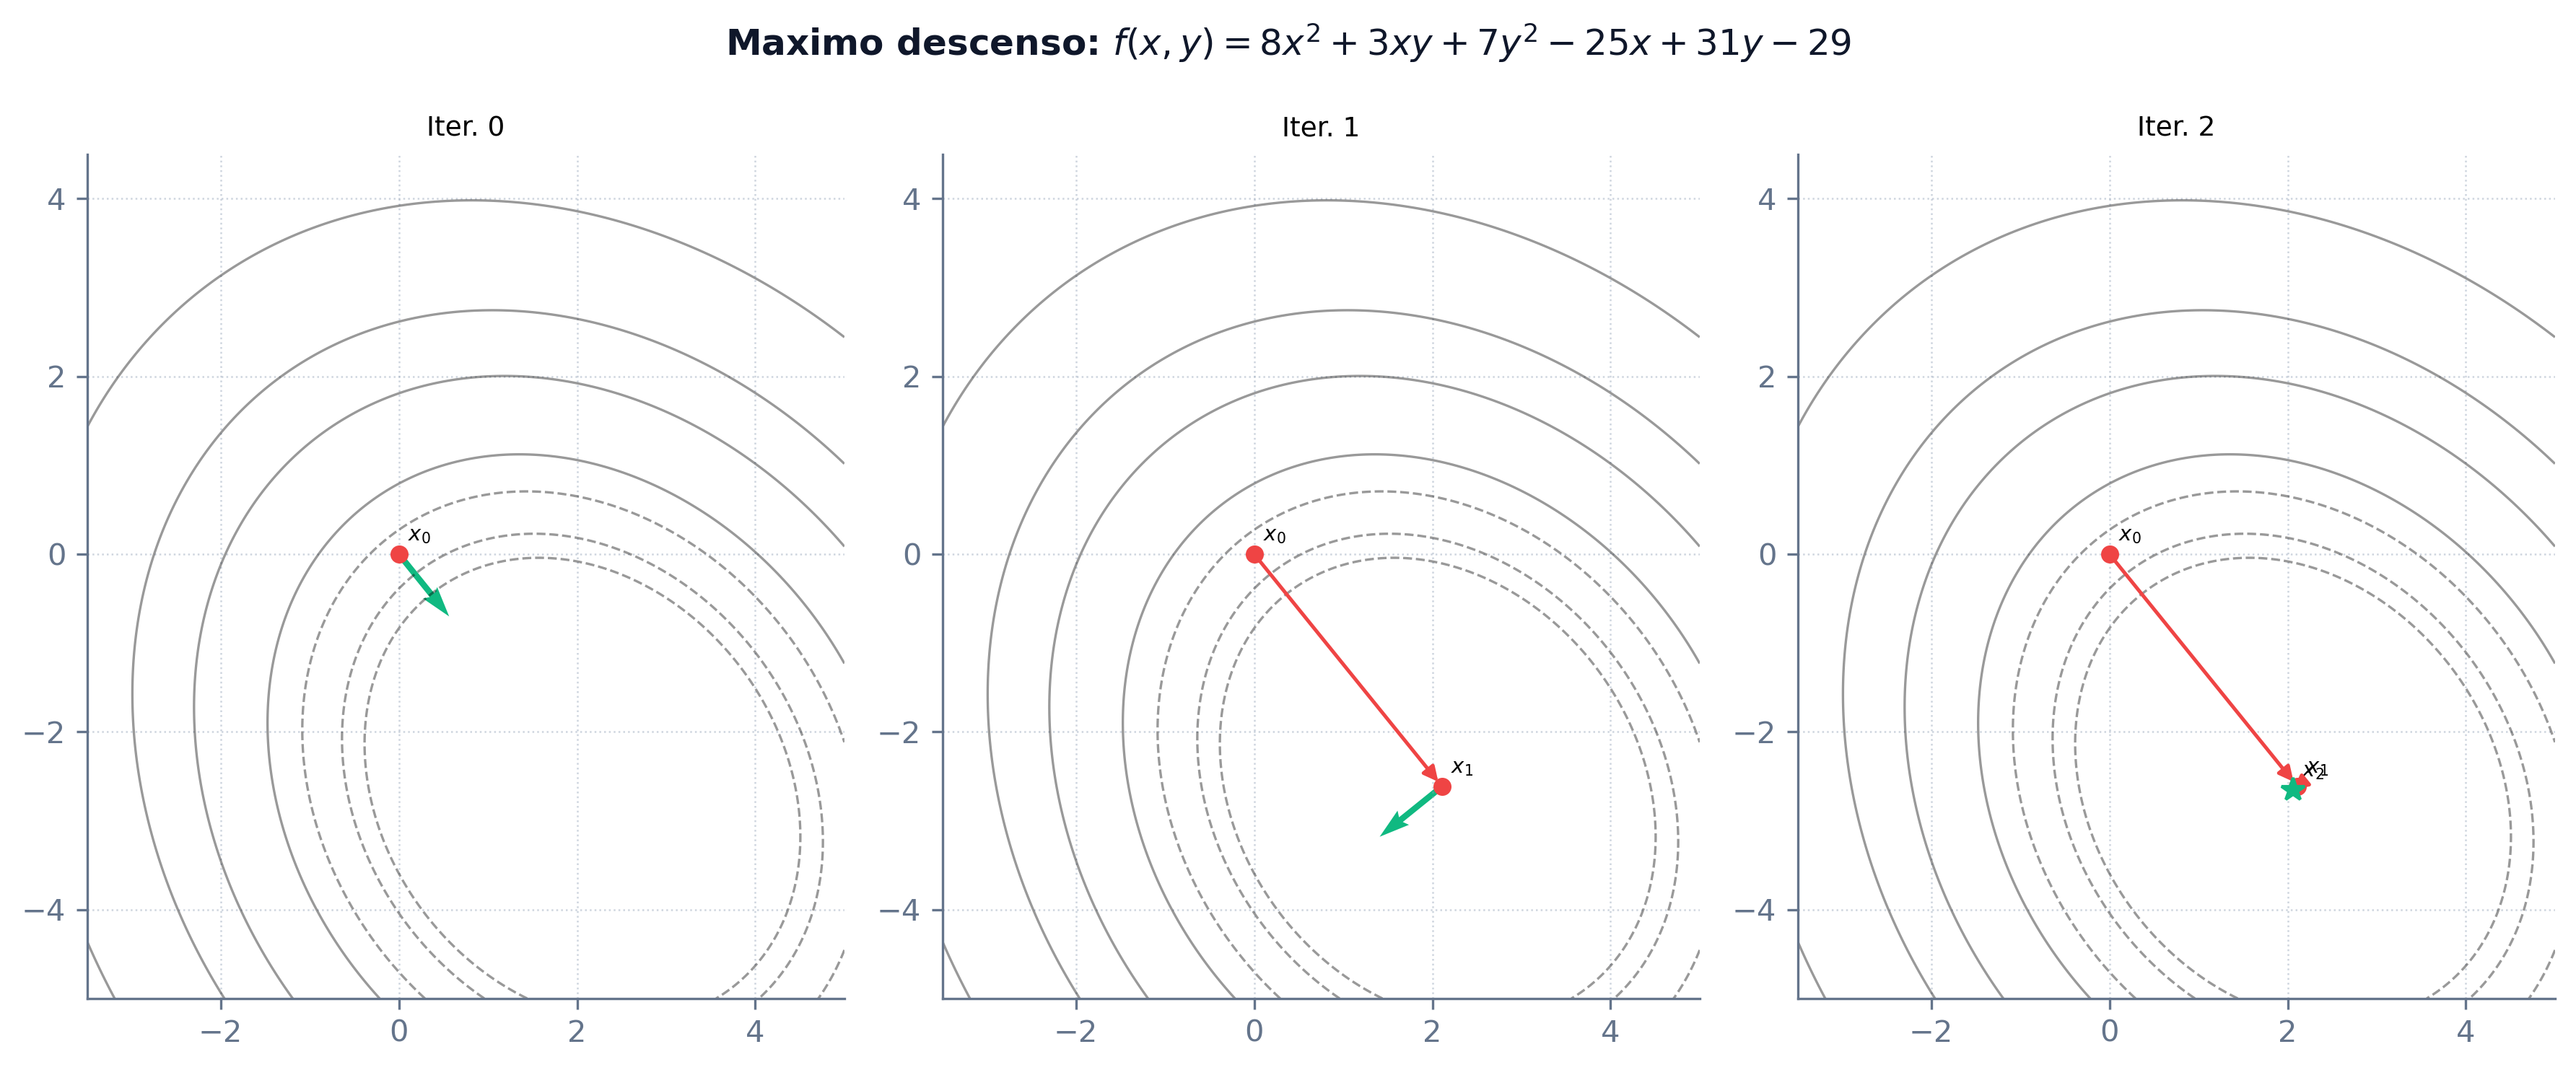
\includegraphics[width=1\linewidth,height=\textheight,keepaspectratio]{images/steepest_descent_pasos.png}

}

\caption{\label{fig-steepest-descent}Máximo descenso: secuencia de
iteraciones mostrando trayectoria ortogonal sobre las curvas de nivel
elípticas}

\end{figure}%

\end{tcolorbox}

\subsection{Métodos de Newton multivariante y
BFGS}\label{muxe9todos-de-newton-multivariante-y-bfgs}

El \textbf{Método de Newton Multivariante} incorpora información de
segundo orden sobre la curvatura de la superficie para acelerar
drásticamente el proceso de convergencia. En lugar de limitarse a una
aproximación lineal, aproxima la función objetivo en el entorno del
punto actual \(x_k\) mediante su desarrollo cuadrático de Taylor:
\[ m_k(p) = f(x_k) + \nabla f(x_k)^T p + \frac{1}{2} p^T \nabla^2 f(x_k) p \]
donde \(p \in \mathbb{R}^n\) es el vector de desplazamiento. Para
calcular el desplazamiento que minimiza este modelo cuadrático local, se
iguala su gradiente a cero respecto a \(p\):
\[ \nabla_p m_k(p) = \nabla f(x_k) + \nabla^2 f(x_k) p = 0 \implies \nabla^2 f(x_k) p = -\nabla f(x_k) \]
Despejando el vector de dirección \(p\), denominado \textbf{dirección de
Newton} (\(d_k\)), y aplicando el paso al punto actual, se obtiene la
regla de actualización clásica:
\[x_{k+1} = x_k - [\nabla^2 f(x_k)]^{-1} \nabla f(x_k)\] Si la función
objetivo es cuadrática y estrictamente convexa, el método de Newton
localiza el mínimo global del sistema en una sola iteración desde
cualquier punto inicial. Para funciones no lineales generales, presenta
una \textbf{convergencia cuadrática local} (orden 2), lo que significa
que el número de cifras significativas exactas prácticamente se duplica
en cada iteración cuando se encuentra cerca de la solución.

En formulaciones prácticas, para evitar divergencias cuando la
estimación inicial no es cercana al óptimo, se utiliza el \textbf{método
de Newton amortiguado} (\emph{damped Newton}), introduciendo un tamaño
de paso \(\alpha_k\) regulado por búsqueda lineal:
\[ x_{k+1} = x_k - \alpha_k [\nabla^2 f(x_k)]^{-1} \nabla f(x_k) \]

A pesar de su velocidad de convergencia, el método de Newton puro
presenta tres limitaciones importantes:

\begin{itemize}
\tightlist
\item
  \textbf{Coste computacional elevado}: En cada iteración se debe
  calcular analítica o numéricamente la matriz hessiana completa
  (\(n(n+1)/2\) derivadas segundas) y resolver un sistema de ecuaciones
  lineales \(n \times n\), lo que supone un coste computacional de
  \(O(n^3)\) operaciones.
\item
  \textbf{Exigencia de convexidad}: Requiere que la matriz hessiana
  \(\nabla^2 f(x_k)\) sea estrictamente definida positiva en cada paso
  para garantizar que la dirección de Newton apunte en sentido de
  descenso. Si el algoritmo entra en una región cóncava o próxima a un
  punto de silla, la dirección puede orientarse hacia un máximo o perder
  la propiedad de descenso.
\item
  \textbf{Convergencia puramente local}: La garantía formal de
  convergencia rápida solo es válida si el punto inicial \(x_0\) se
  encuentra lo bastante próximo al punto óptimo.
\end{itemize}

Los \textbf{Métodos Cuasi-Newton (BFGS)} resuelven estas limitaciones de
forma elegante. En lugar de evaluar y factorizar la matriz hessiana
exacta en cada iteración, construyen secuencialmente una aproximación
simétrica y definida positiva de la inversa de la hessiana, denotada por
\(H_k \approx [\nabla^2 f(x_k)]^{-1}\). Esta matriz se actualiza
utilizando únicamente las variaciones de posiciones y de gradientes
entre dos iteraciones consecutivas, imponiendo la \textbf{ecuación de la
secante}: \[H_{k+1} y_k = s_k\] donde \(s_k = x_{k+1} - x_k\) representa
el desplazamiento del punto e
\(y_k = \nabla f(x_{k+1}) - \nabla f(x_k)\) cuantifica la variación del
gradiente.

El algoritmo \textbf{BFGS} (desarrollado de forma independiente por
Broyden, Fletcher, Goldfarb y Shanno) actualiza la matriz aproximada
mediante la expresión:
\[H_{k+1} = (I - \rho_k s_k y_k^T) H_k (I - \rho_k y_k s_k^T) + \rho_k s_k s_k^T\]
donde \(\rho_k = 1 / (y_k^T s_k)\). Si el tamaño de paso en la búsqueda
lineal satisface las condiciones de Wolfe, se garantiza matemáticamente
que la matriz \(H_{k+1}\) se mantenga simétrica y estrictamente definida
positiva, asegurando direcciones de descenso en cada paso. Este enfoque
proporciona una tasa de \textbf{convergencia superlineal} con un coste
computacional de tan solo \(O(n^2)\) operaciones por iteración (Nocedal
y Wright 2006; Luenberger y Ye 2015).

Para sintetizar la progresión conceptual de los métodos multivariantes
sin restricciones estudiados en este tema, la siguiente tabla compara
sus rasgos operativos y computacionales:

\begin{longtable}[]{@{}
  >{\raggedright\arraybackslash}p{(\linewidth - 8\tabcolsep) * \real{0.2000}}
  >{\raggedright\arraybackslash}p{(\linewidth - 8\tabcolsep) * \real{0.2000}}
  >{\raggedright\arraybackslash}p{(\linewidth - 8\tabcolsep) * \real{0.2000}}
  >{\raggedright\arraybackslash}p{(\linewidth - 8\tabcolsep) * \real{0.2000}}
  >{\raggedright\arraybackslash}p{(\linewidth - 8\tabcolsep) * \real{0.2000}}@{}}
\toprule\noalign{}
\begin{minipage}[b]{\linewidth}\raggedright
Algoritmo
\end{minipage} & \begin{minipage}[b]{\linewidth}\raggedright
Orden y datos requeridos
\end{minipage} & \begin{minipage}[b]{\linewidth}\raggedright
Coste por paso
\end{minipage} & \begin{minipage}[b]{\linewidth}\raggedright
Tasa de convergencia
\end{minipage} & \begin{minipage}[b]{\linewidth}\raggedright
Requisitos de curvatura y robustez
\end{minipage} \\
\midrule\noalign{}
\endhead
\bottomrule\noalign{}
\endlastfoot
\textbf{Coordenadas Cíclicas} & Orden 0 (solo evalúa \(f(x)\)) &
\(O(n)\) búsquedas 1D & Lenta (sublineal) & No requiere derivadas;
vulnerable a acoplamiento cruzado \\
\textbf{Máximo Descenso} & Orden 1 (\(f(x)\) y gradiente \(\nabla f\)) &
\(O(n)\) más búsqueda 1D & Lineal & Muy robusto con búsqueda lineal;
sufre zigzag en elipses alargadas \\
\textbf{Newton Clásico} & Orden 2 (\(f, \nabla f\) y hessiana
\(\nabla^2 f\)) & \(O(n^3)\) (sistema lineal) & Cuadrática (local) & Muy
rápido cerca del óptimo; exige hessiana definida positiva \\
\textbf{Cuasi-Newton (BFGS)} & Orden 1 (\(f(x)\) y gradientes sucesivos)
& \(O(n^2)\) (álgebra matricial) & Superlineal & Excelente equilibrio
práctico; preserva siempre definida positiva \\
\end{longtable}

\chapter{Análisis convexo}\label{anuxe1lisis-convexo}

El \textbf{análisis convexo} constituye la columna vertebral de la
optimización matemática moderna. Históricamente, la optimización estuvo
dominada por el paradigma de la linealidad frente a la no linealidad.
Sin embargo, a finales del siglo XX se produjo un cambio de paradigma
fundamental, resumido por el matemático R. Tyrrell Rockafellar:
\emph{``la divisoria fundamental en optimización no es entre linealidad
y no linealidad, sino entre convexidad y no convexidad''} (Rockafellar
1970). Bajo la hipótesis de convexidad, cualquier óptimo local se
convierte de manera natural en un óptimo global (Boyd y Vandenberghe
2004). Esta propiedad crucial no solo simplifica la búsqueda teórica de
soluciones, sino que garantiza la convergencia fiable y veloz de los
algoritmos numéricos, evitando que queden atrapados en mínimos locales
subóptimos.

En este capítulo, estudiaremos los conjuntos convexos y las operaciones
que preservan esta propiedad, las caracterizaciones de primer y segundo
orden para funciones convexas diferenciables y no diferenciables
(subgradientes), las propiedades fundamentales de sus extremos y las
generalizaciones teóricas de la convexidad (cuasi-convexidad y
pseudo-convexidad).

\begin{tcolorbox}[enhanced jigsaw, toprule=.15mm, opacitybacktitle=0.6, coltitle=black, colbacktitle=quarto-callout-important-color!10!white, title=\textcolor{quarto-callout-important-color}{\faExclamation}\hspace{0.5em}{Objetivos de aprendizaje}, arc=.35mm, rightrule=.15mm, toptitle=1mm, breakable, bottomtitle=1mm, titlerule=0mm, colback=white, opacityback=0, leftrule=.75mm, colframe=quarto-callout-important-color-frame, left=2mm, bottomrule=.15mm]

Al finalizar este capítulo, serás capaz de:

\begin{enumerate}
\def\labelenumi{\arabic{enumi}.}
\tightlist
\item
  \textbf{Identificar y demostrar} si un conjunto dado en
  \(\mathbb{R}^n\) es convexo aplicando la definición o las propiedades
  algebraicas de conservación.
\item
  \textbf{Diferenciar} entre combinaciones lineales, afines, cónicas y
  convexas, analizando la estructura geométrica de sus envolturas.
\item
  \textbf{Comprender e interpretar} los Teoremas de Separación de
  Hiperplanos y del Hiperplano de Soporte.
\item
  \textbf{Caracterizar la convexidad de funciones} mediante las
  propiedades del epigrafo, los conjuntos de nivel y las
  caracterizaciones de primer y segundo orden (gradiente y hessiana).
\item
  \textbf{Calcular el subdiferencial} de funciones convexas no
  diferenciables en puntos singulares de esquina o codo, y aplicar el
  cálculo de subgradientes.
\item
  \textbf{Aplicar el Teorema Fundamental de la Optimización Convexa}
  para deconstruir y verificar la globalidad y unicidad de los mínimos.
\item
  \textbf{Clasificar y relacionar} las funciones cuasi-convexas,
  pseudo-convexas y sus variantes, comprendiendo sus implicaciones en la
  optimización restringida.
\end{enumerate}

\end{tcolorbox}

\section{Conjuntos convexos}\label{conjuntos-convexos}

El estudio de la convexidad se inicia con la caracterización geométrica
de los conjuntos sobre los que se definen los problemas de optimización.
Intuitivamente, un conjunto es convexo si no presenta ``entrantes'' o
cavidades, de modo que la conexión recta entre cualquier pareja de sus
puntos está totalmente contenida en él, tal y como se ilustra en la
Figura~\ref{fig-conjuntos-convexos}.

Formalmente, definimos un \textbf{conjunto convexo}
\(\mathcal{S} \subseteq \mathbb{R}^n\) como aquel que cumple que, para
todo par de puntos \(x_1, x_2 \in \mathcal{S}\) y cualquier parámetro de
ponderación \(\lambda \in (0, 1)\), el segmento intermedio también
pertenece al conjunto, es decir:
\[ \lambda x_1 + (1 - \lambda) x_2 \in \mathcal{S} \]

\begin{figure}

\centering{

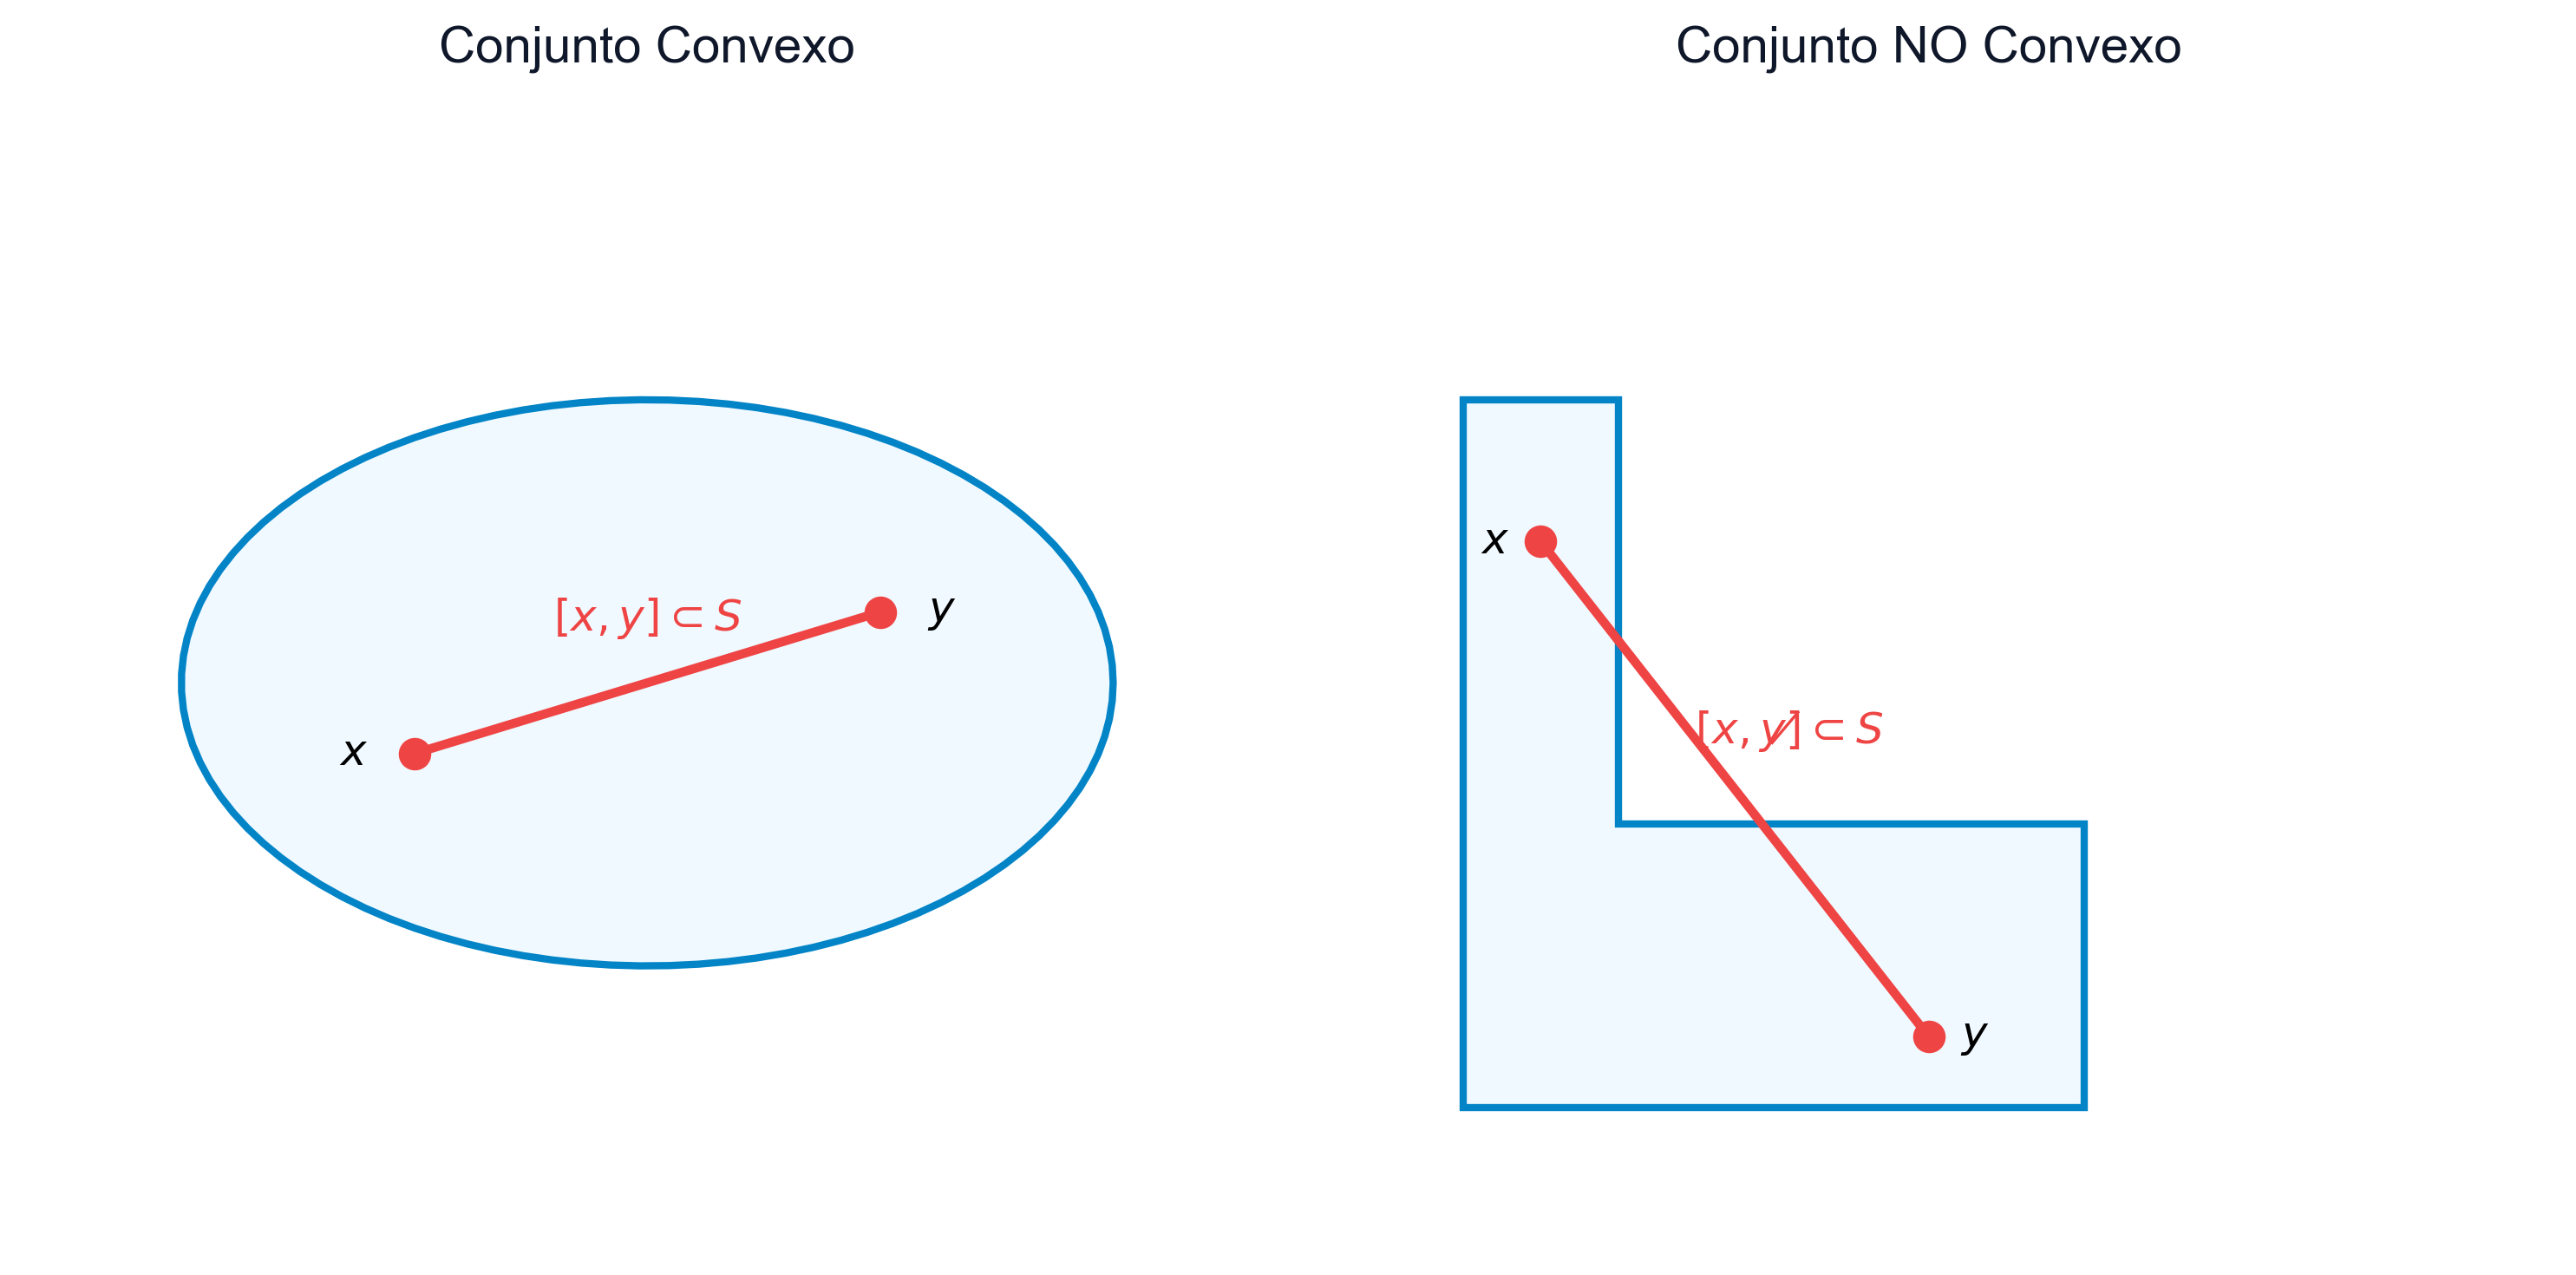
\includegraphics[width=0.8\linewidth,height=\textheight,keepaspectratio]{images/conjuntos_convexos.png}

}

\caption{\label{fig-conjuntos-convexos}Comparación entre un conjunto
convexo (izquierda) y un conjunto no convexo (derecha)}

\end{figure}%

Esta noción geométrica de segmento se puede generalizar a conjuntos de
múltiples puntos a través de diferentes clases de combinaciones
algebraicas, cuyas propiedades estructuran el espacio lineal. Decimos
que un punto \(x \in \mathbb{R}^n\) es una \textbf{combinación lineal
convexa} de un conjunto finito de puntos
\(\{x_1, \dots, x_k\} \subset \mathbb{R}^n\) si puede expresarse de la
forma:
\[ x = \sum_{i=1}^k \lambda_i x_i \quad \text{con} \quad \lambda_i \ge 0 \quad \text{y} \quad \sum_{i=1}^k \lambda_i = 1 \]

Si eliminamos la condición de no negatividad de los coeficientes,
exigiendo únicamente que sumen uno (\(\lambda_i \in \mathbb{R}\) con
\(\sum_{i=1}^k \lambda_i = 1\)), obtenemos una \textbf{combinación
afín}, la cual genera subespacios afines como rectas o planos. Por otro
lado, si exigimos únicamente la no negatividad de los coeficientes pero
no que sumen uno (\(\lambda_i \ge 0\)), se define una
\textbf{combinación cónica}, responsable de generar conos convexos.
Finalmente, si eliminamos ambas restricciones permitiendo cualquier
\(\lambda_i \in \mathbb{R}\), recuperamos la noción de
\textbf{combinación lineal} ordinaria, que da origen a los subespacios
vectoriales tradicionales.

\begin{tcolorbox}[enhanced jigsaw, toprule=.15mm, opacitybacktitle=0.6, coltitle=black, colbacktitle=quarto-callout-tip-color!10!white, title=\textcolor{quarto-callout-tip-color}{\faLightbulb}\hspace{0.5em}{Ejemplos: Conjuntos convexos básicos}, arc=.35mm, rightrule=.15mm, toptitle=1mm, breakable, bottomtitle=1mm, titlerule=0mm, colback=white, opacityback=0, leftrule=.75mm, colframe=quarto-callout-tip-color-frame, left=2mm, bottomrule=.15mm]

A continuación se presentan algunas de las estructuras convexas más
elementales y recurrentes en optimización:

\begin{itemize}
\tightlist
\item
  \textbf{Hiperplano}: Dado un vector normal no nulo
  \(p \in \mathbb{R}^n\) y un escalar \(\alpha \in \mathbb{R}\),
  representa una superficie plana de dimensión \(n-1\) definida por:
  \[ \mathcal{H} = \{ x \in \mathbb{R}^n \mid p^T x = \alpha \} \]
\item
  \textbf{Semiespacio Cerrado}: Representa la región del espacio situada
  en uno de los lados de un hiperplano:
  \[ \mathcal{H}^- = \{ x \in \mathbb{R}^n \mid p^T x \le \alpha \} \]
\item
  \textbf{Poliedro o Politopo Convexo}: La intersección de un número
  finito de semiespacios cerrados, dada por:
  \[ \mathcal{P} = \{ x \in \mathbb{R}^n \mid A x \le b \} \] Esta
  estructura constituye la región factible típica de los problemas de
  programación lineal. Sus esquinas o vértices se denominan
  \textbf{puntos extremos}.
\item
  \textbf{Bola Métrica}: Una bola cerrada en \(\mathbb{R}^n\) con centro
  en \(x_0\) y radio \(r \ge 0\) definida bajo cualquier norma
  \(\|\cdot\|\):
  \[ \mathcal{B}_r(x_0) = \{ x \in \mathbb{R}^n \mid \|x - x_0\| \le r \} \]
\end{itemize}

\end{tcolorbox}

Para poder operar y construir geometrías más complejas, es fundamental
conocer las operaciones algebraicas y conjuntistas que preservan la
propiedad de convexidad.

\begin{tcolorbox}[enhanced jigsaw, toprule=.15mm, opacitybacktitle=0.6, coltitle=black, colbacktitle=quarto-callout-note-color!10!white, title=\textcolor{quarto-callout-note-color}{\faInfo}\hspace{0.5em}{Lema: Conservación de la convexidad}, arc=.35mm, rightrule=.15mm, toptitle=1mm, breakable, bottomtitle=1mm, titlerule=0mm, colback=white, opacityback=0, leftrule=.75mm, colframe=quarto-callout-note-color-frame, left=2mm, bottomrule=.15mm]

Sean \(\mathcal{S}_1\) y \(\mathcal{S}_2\) dos conjuntos convexos en
\(\mathbb{R}^n\). Las siguientes estructuras también son conjuntos
convexos:

\begin{enumerate}
\def\labelenumi{\arabic{enumi}.}
\tightlist
\item
  \textbf{Intersección}: \[ \mathcal{S}_1 \cap \mathcal{S}_2 \] (Esta
  propiedad se extiende a la intersección de una familia infinita o
  arbitraria de conjuntos convexos).
\item
  \textbf{Suma Directa}:
  \[ \mathcal{S}_1 \oplus \mathcal{S}_2 = \{ x_1 + x_2 \mid x_1 \in \mathcal{S}_1, \ x_2 \in \mathcal{S}_2 \} \]
\item
  \textbf{Diferencia Directa}:
  \[ \mathcal{S}_1 \ominus \mathcal{S}_2 = \{ x_1 - x_2 \mid x_1 \in \mathcal{S}_1, \ x_2 \in \mathcal{S}_2 \} \]
\end{enumerate}

\emph{Demostración}: 1. \textbf{Intersección}: Sean
\(x, y \in \mathcal{S}_1 \cap \mathcal{S}_2\) y \(\lambda \in (0, 1)\).
Como \(x, y \in \mathcal{S}_1\) y \(\mathcal{S}_1\) es convexo, entonces
\(\lambda x + (1-\lambda)y \in \mathcal{S}_1\). Igualmente, como
\(x, y \in \mathcal{S}_2\) y \(\mathcal{S}_2\) es convexo,
\(\lambda x + (1-\lambda)y \in \mathcal{S}_2\). Por tanto, el punto
intermedio pertenece a la intersección. 2. \textbf{Suma Directa}: Sean
\(z_1, z_2 \in \mathcal{S}_1 \oplus \mathcal{S}_2\). Entonces
\(z_1 = x_1 + y_1\) y \(z_2 = x_2 + y_2\) para ciertos
\(x_1, x_2 \in \mathcal{S}_1\) e \(y_1, y_2 \in \mathcal{S}_2\). Para
cualquier \(\lambda \in (0, 1)\):
\[ \lambda z_1 + (1-\lambda)z_2 = (\lambda x_1 + (1-\lambda)x_2) + (\lambda y_1 + (1-\lambda)y_2) \]
Por la convexidad de \(\mathcal{S}_1\) y \(\mathcal{S}_2\), el primer
sumando pertenece a \(\mathcal{S}_1\) y el segundo a \(\mathcal{S}_2\).
Por tanto, la combinación pertenece a
\(\mathcal{S}_1 \oplus \mathcal{S}_2\). 3. \textbf{Diferencia Directa}:
Se demuestra de forma análoga a la suma directa considerando la resta de
elementos. \(\blacksquare\)

\end{tcolorbox}

\subsection{Envoltura convexa y
símplices}\label{envoltura-convexa-y-suxedmplices}

La envoltura convexa es una construcción matemática fundamental que
permite obtener el conjunto convexo más pequeño posible que contiene a
un conjunto de puntos arbitrario. Intuitivamente, se puede imaginar como
el contorno que formaría una banda elástica si se tensara alrededor de
un conjunto de clavos clavados en una tabla, tal y como se ilustra en la
Figura~\ref{fig-envoltura-convexa}.

Definimos formalmente la \textbf{envoltura convexa}
\(\mathcal{H}(\mathcal{S})\) de un conjunto \(\mathcal{S}\) como el
conjunto formado por todas las combinaciones lineales convexas posibles
de puntos pertenecientes a \(\mathcal{S}\):
\[ \mathcal{H}(\mathcal{S}) = \left\{ x = \sum_{j=1}^k \lambda_j x_j \;\middle|\; x_j \in \mathcal{S}, \ \lambda_j \ge 0, \ \sum_{j=1}^k \lambda_j = 1 \right\} \]

\begin{figure}

\centering{

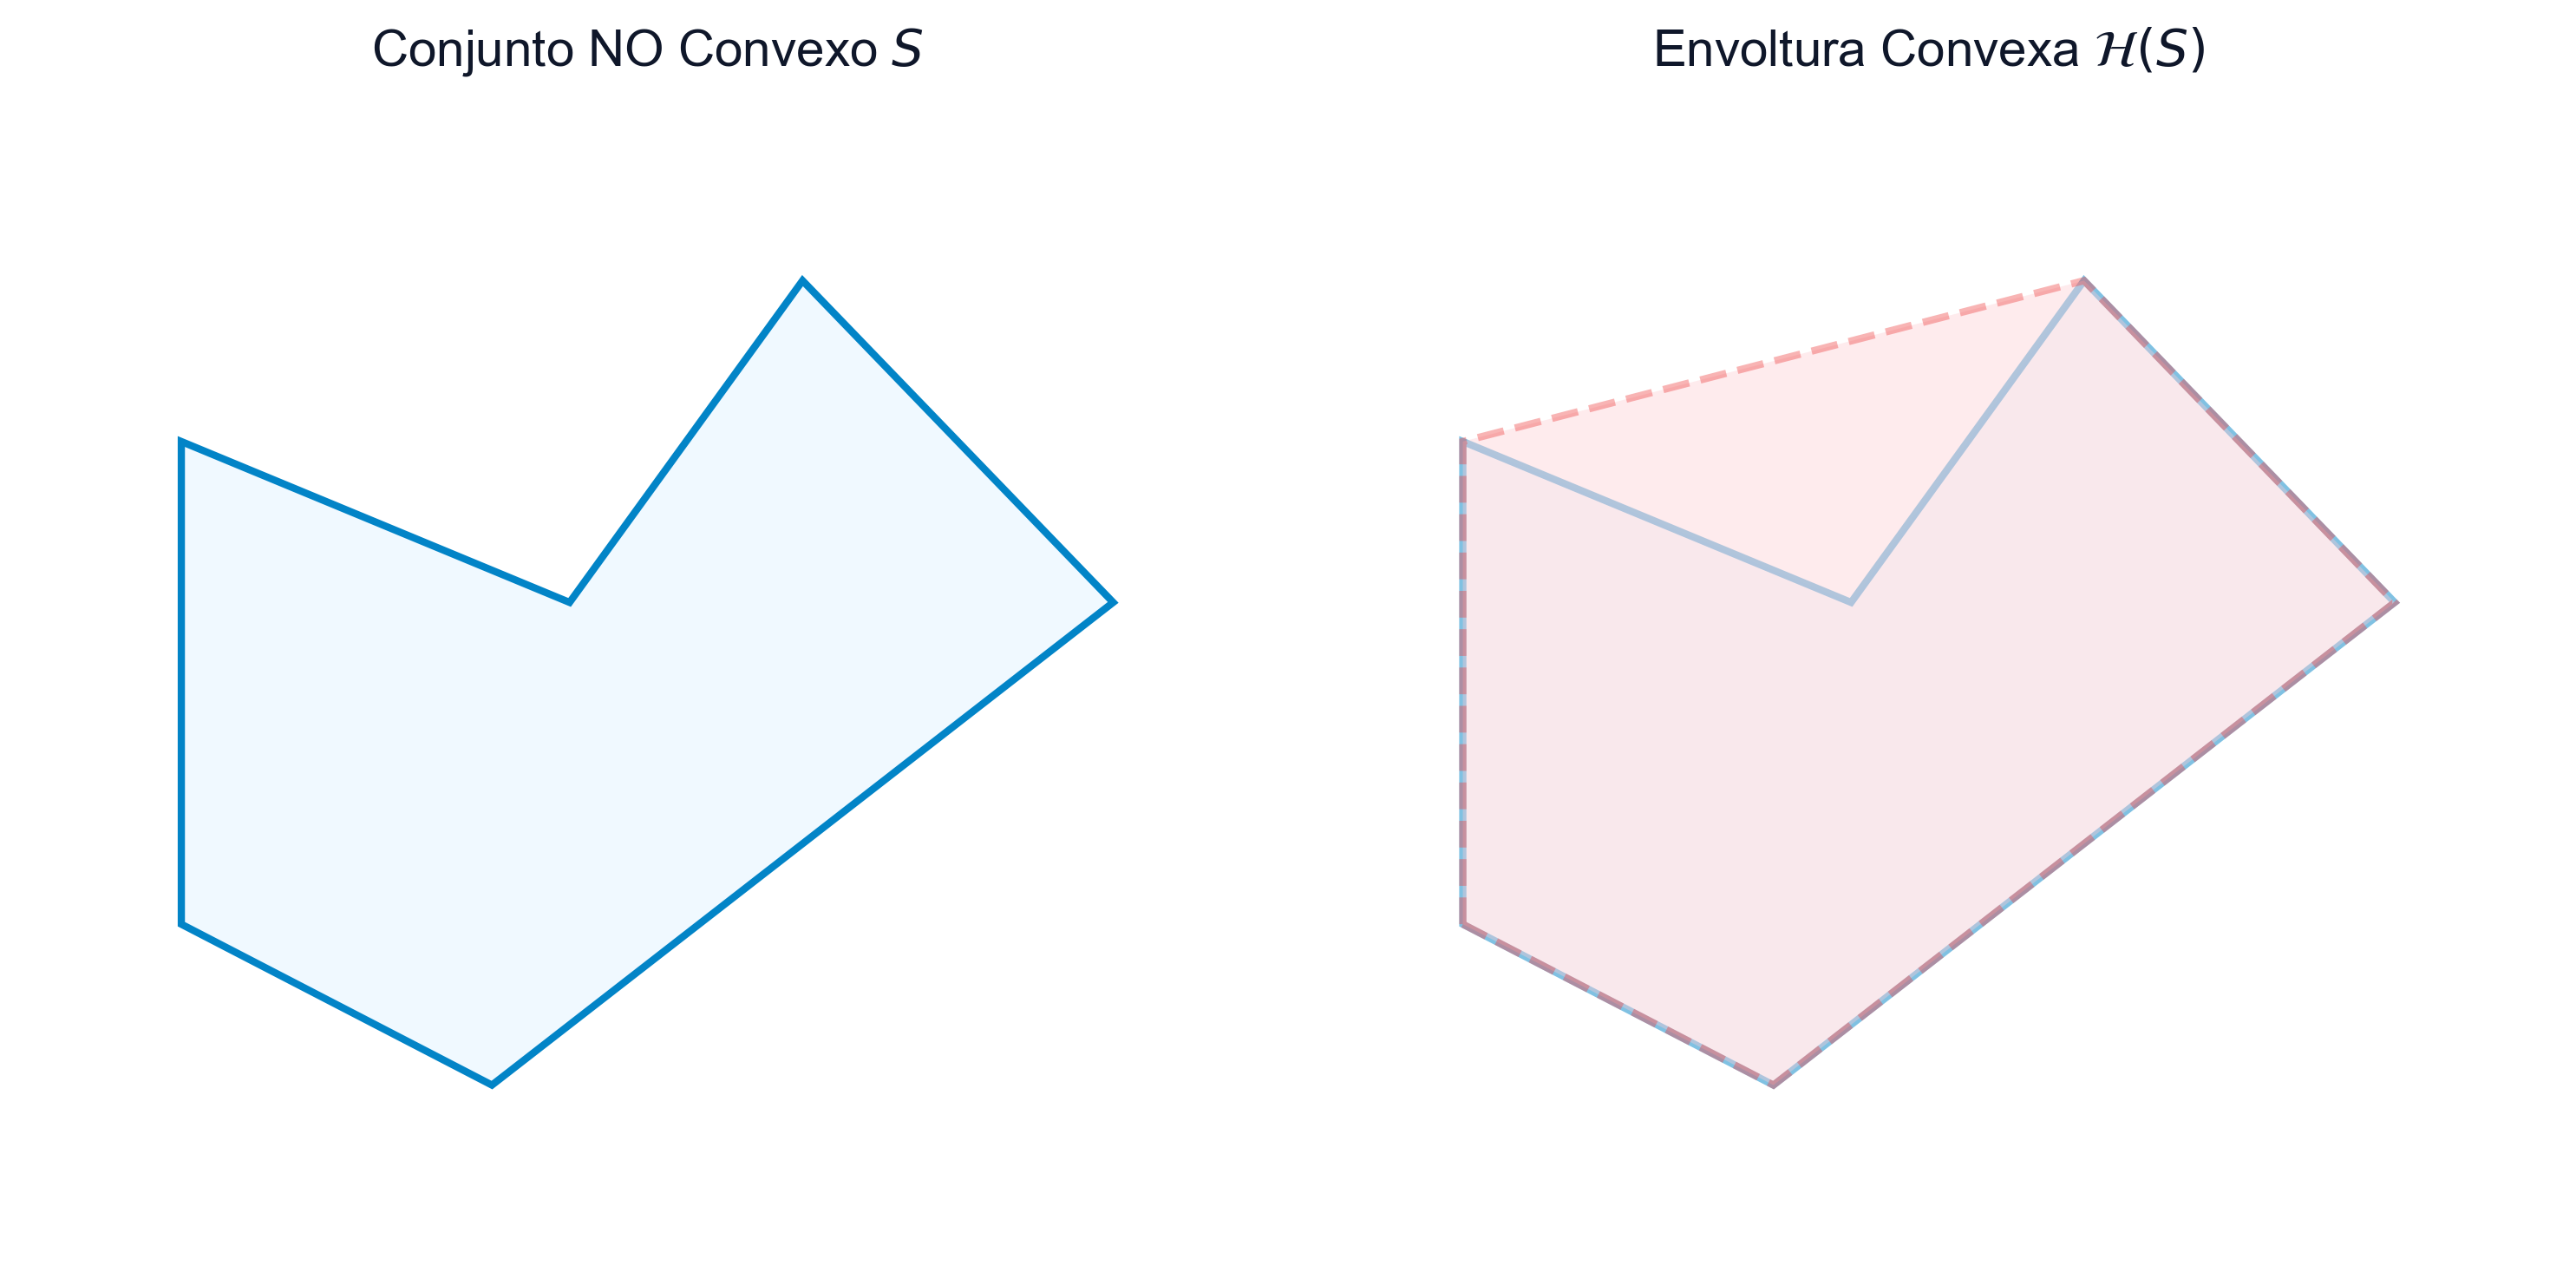
\includegraphics[width=0.8\linewidth,height=\textheight,keepaspectratio]{images/envoltura_convexa.png}

}

\caption{\label{fig-envoltura-convexa}Representación de un conjunto no
convexo (izquierda) y su envoltura convexa (derecha)}

\end{figure}%

\begin{tcolorbox}[enhanced jigsaw, toprule=.15mm, opacitybacktitle=0.6, coltitle=black, colbacktitle=quarto-callout-important-color!10!white, title=\textcolor{quarto-callout-important-color}{\faExclamation}\hspace{0.5em}{Teorema: Minimalidad de la envoltura convexa}, arc=.35mm, rightrule=.15mm, toptitle=1mm, breakable, bottomtitle=1mm, titlerule=0mm, colback=white, opacityback=0, leftrule=.75mm, colframe=quarto-callout-important-color-frame, left=2mm, bottomrule=.15mm]

La envoltura convexa \(\mathcal{H}(\mathcal{S})\) es el menor conjunto
convexo que contiene al conjunto \(\mathcal{S}\).

\emph{Demostración}: Sea \(\mathcal{C}\) any conjunto convexo que
contiene a \(\mathcal{S}\) (es decir,
\(\mathcal{S} \subseteq \mathcal{C}\)). Supongamos por reducción al
absurdo que existe un punto \(x \in \mathcal{H}(\mathcal{S})\) tal que
\(x \notin \mathcal{C}\). Como \(x \in \mathcal{H}(\mathcal{S})\), se
puede escribir como una combinación lineal convexa
\(x = \sum_{j=1}^k \lambda_j x_j\) donde cada \(x_j \in \mathcal{S}\).
Dado que \(\mathcal{S} \subseteq \mathcal{C}\), se deduce que todos los
puntos generadores \(x_j\) pertenecen a \(\mathcal{C}\). Como
\(\mathcal{C}\) es convexo por hipótesis, cualquier combinación lineal
convexa de sus elementos debe pertenecer a él, lo que obliga a que
\(x \in \mathcal{C}\), contradiciendo la suposición inicial.
\(\blacksquare\)

\end{tcolorbox}

Cuando limitamos la generación a conjuntos de puntos con propiedades de
independencia afín, entramos en la categoría de los símplices y
politopos convexos. Un \textbf{politopo convexo} es el conjunto obtenido
mediante la envoltura convexa de un número finito de puntos en
\(\mathbb{R}^n\). Si estos puntos de generación son afínmente
independientes, el politopo se denomina \textbf{símplex (o simplex)}. En
particular, un símplex en \(\mathbb{R}^1\) corresponde a un segmento
cerrado, en \(\mathbb{R}^2\) a un triángulo y en \(\mathbb{R}^3\) a un
tetraedro, tal y como se ilustra en la
Figura~\ref{fig-politopo-simplex}.

\begin{figure}

\centering{

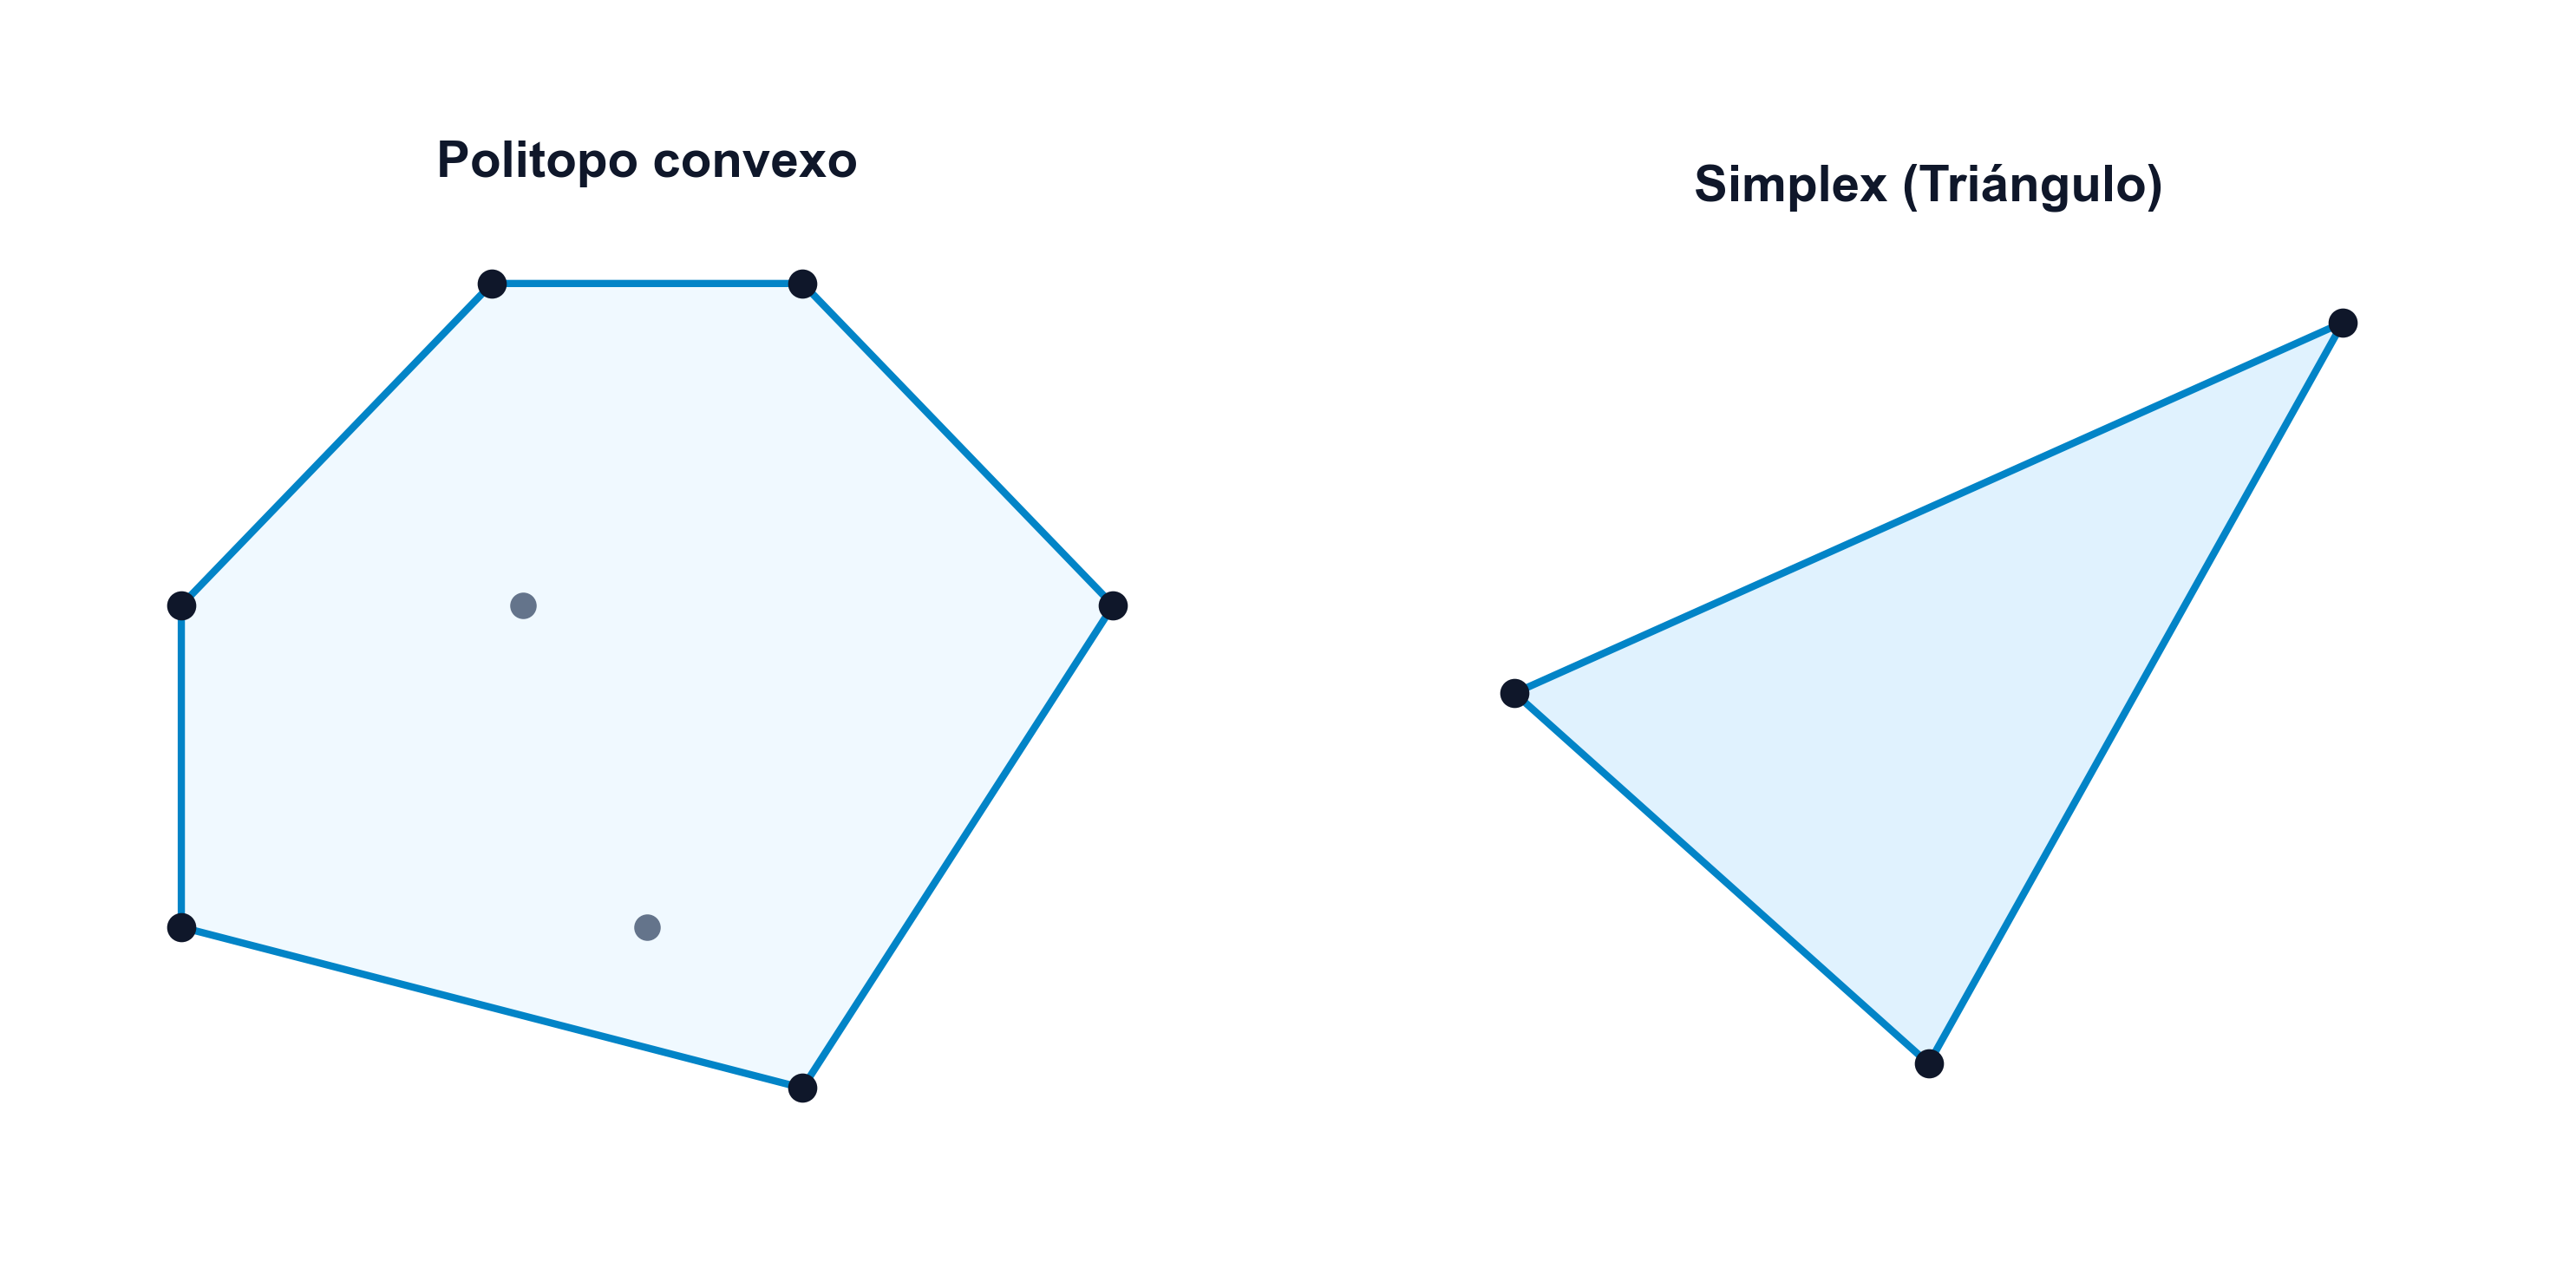
\includegraphics[width=0.8\linewidth,height=\textheight,keepaspectratio]{images/politopo_simplex.png}

}

\caption{\label{fig-politopo-simplex}Ejemplo de un Politopo convexo
generado por un número finito de puntos (izquierda) y un Simplex
bidimensional o triángulo generado por tres puntos afínmente
independientes (derecha)}

\end{figure}%

\subsection{Puntos extremos y optimización en
poliedros}\label{sec-puntos-extremos}

Para conjuntos convexos generales, y en particular para poliedros, es de
vital importancia identificar aquellos puntos frontera singulares que no
pueden expresarse como combinaciones intermedias de otros. Un
\textbf{punto extremo} es aquel elemento \(x\) perteneciente a un
conjunto convexo \(\mathcal{S}\) que no puede expresarse como una
combinación lineal convexa de otros dos puntos distintos del conjunto.
Es decir, no existe ningún par de puntos distintos
\(x_1, x_2 \in \mathcal{S}\) (ambos diferentes de \(x\)) y ningún
parámetro \(\lambda \in (0, 1)\) tales que:
\[ x = \lambda x_1 + (1-\lambda)x_2 \] En el contexto de los poliedros,
los puntos extremos coinciden exactamente con la noción geométrica de
\emph{vértices}.

\begin{tcolorbox}[enhanced jigsaw, toprule=.15mm, opacitybacktitle=0.6, coltitle=black, colbacktitle=quarto-callout-important-color!10!white, title=\textcolor{quarto-callout-important-color}{\faExclamation}\hspace{0.5em}{Teorema: Maximización en poliedros}, arc=.35mm, rightrule=.15mm, toptitle=1mm, breakable, bottomtitle=1mm, titlerule=0mm, colback=white, opacityback=0, leftrule=.75mm, colframe=quarto-callout-important-color-frame, left=2mm, bottomrule=.15mm]

Sea \(f: \mathbb{R}^n \to \mathbb{R}\) una función convexa y sea
\(\mathcal{S}\) un poliedro compacto (cerrado y acotado) no vacío en
\(\mathbb{R}^n\). Entonces, el problema de maximizar \(f(x)\) sujeto a
\(x \in \mathcal{S}\) alcanza su óptimo global en al menos uno de los
puntos extremos de \(\mathcal{S}\).

\emph{Demostración}: Dado que \(f\) es convexa en un dominio compacto
\(\mathcal{S}\), es continua en dicho dominio. Por el Teorema de
Weierstrass, existe un punto \(x' \in \mathcal{S}\) donde \(f\) alcanza
su máximo global.

Por el Teorema de Representación de Minkowski-Weyl, todo punto de un
poliedro compacto \(\mathcal{S}\) se puede expresar como una combinación
lineal convexa de sus puntos extremos \(\{x_1, \dots, x_k\}\):
\[ x' = \sum_{j=1}^k \lambda_j x_j, \qquad \text{con } \lambda_j \ge 0, \quad \sum_{j=1}^k \lambda_j = 1 \]
Aplicando la propiedad de convexidad de \(f\) (generalizada por la
desigualdad de Jensen):
\[ f(x') = f\left(\sum_{j=1}^k \lambda_j x_j\right) \le \sum_{j=1}^k \lambda_j f(x_j) \]
Por otro lado, como \(x'\) es el punto que maximiza \(f\) en
\(\mathcal{S}\), tenemos que \(f(x') \ge f(x_j)\) para todo
\(j = 1, \dots, k\). Al multiplicar estas desigualdades por
\(\lambda_j \ge 0\) y sumarlas:
\[ f(x') = \sum_{j=1}^k \lambda_j f(x') \ge \sum_{j=1}^k \lambda_j f(x_j) \]
Por tanto, de las dos inecuaciones anteriores se concluye la igualdad
estricta: \[ f(x') = \sum_{j=1}^k \lambda_j f(x_j) \] Esto solo es
posible si \(f(x') = f(x_j)\) para todo índice \(j\) tal que
\(\lambda_j > 0\). En consecuencia, el valor máximo de la función se
alcanza en los puntos extremos correspondientes. \(\blacksquare\)

\end{tcolorbox}

\section{Funciones convexas}\label{funciones-convexas}

El concepto de función convexa constituye uno de los pilares de la
optimización moderna. A diferencia de las funciones lineales, que
describen comportamientos planos o de tasa constante, las funciones
convexas capturan analíticamente la estructura de un cuenco o superficie
curvada hacia arriba. Esta propiedad geométrica garantiza que cualquier
interpolación lineal entre dos puntos de la función siempre
sobreestimará (o igualará) el valor real de la misma.

Formalmente, la definición analítica de convexidad se establece de la
siguiente manera:

Consideremos un conjunto convexo no vacío
\(\mathcal{S} \subseteq \mathbb{R}^n\). Decimos que una función
\(f: \mathcal{S} \to \mathbb{R}\) es \textbf{convexa} si, para todo par
de puntos \(x_1, x_2 \in \mathcal{S}\) y cualquier parámetro de
ponderación \(\lambda \in (0, 1)\), se verifica la inecuación:
\[ f(\lambda x_1 + (1 - \lambda) x_2) \le \lambda f(x_1) + (1 - \lambda) f(x_2) \]
Si esta inecuación se cumple con desigualdad estricta (\(<\)) para
cualquier par de puntos factibles distintos \(x_1 \neq x_2\), decimos
que la función \(f\) es \textbf{estrictamente convexa}. Por otro lado,
la función \(f\) es \textbf{cóncava} si su opuesta \(-f\) es una función
convexa.

Geométricamente, esta definición establece que el segmento de cuerda (o
secante) que une los puntos de la gráfica \((x_1, f(x_1))\) y
\((x_2, f(x_2))\) queda situado por encima o sobre la propia curva de la
función en dicho intervalo, tal y como se ilustra en la
Figura~\ref{fig-funciones-convexidad-concepto}.

\begin{figure}

\centering{

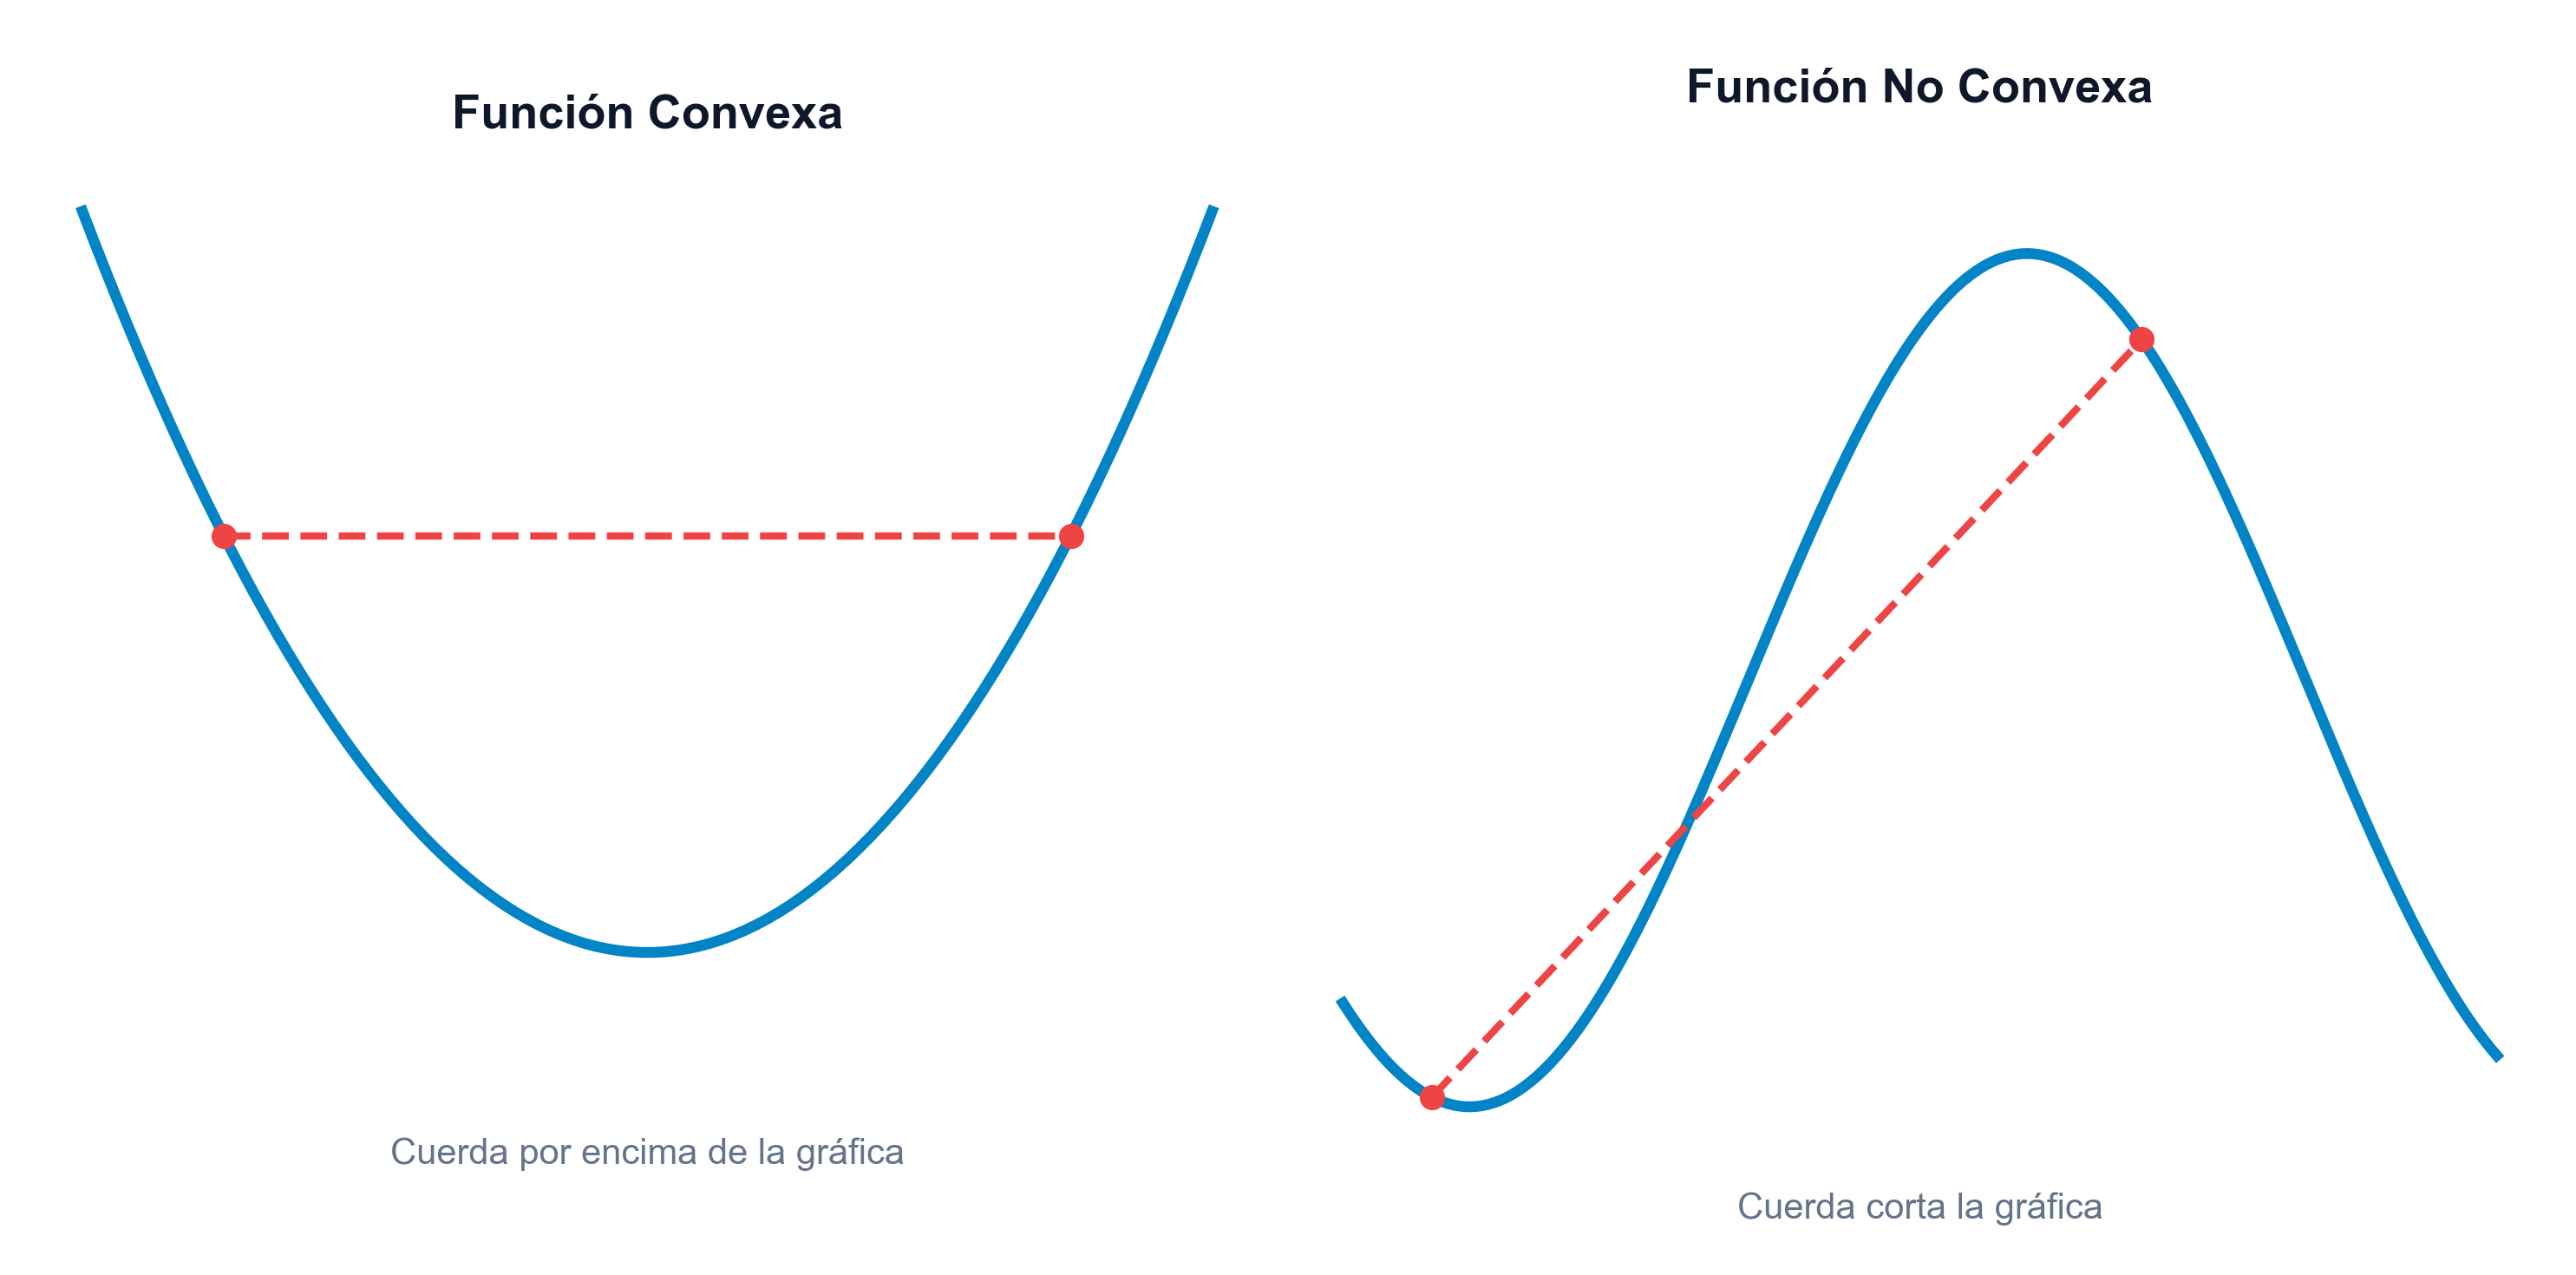
\includegraphics[width=0.8\linewidth,height=\textheight,keepaspectratio]{images/funciones_convexidad_concepto.png}

}

\caption{\label{fig-funciones-convexidad-concepto}Visualización de una
función convexa (izquierda), donde la secante o cuerda queda por encima
de la gráfica, frente a una función no convexa (derecha), donde la
cuerda corta a la curva}

\end{figure}%

Más allá de su interpretación geométrica, una propiedad teórica de gran
alcance para las funciones convexas es que la regularidad algebraica de
la desigualdad de convexidad impone de forma automática la continuidad
de la función en casi todo su dominio, sin necesidad de exigir
diferenciabilidad previa.

\begin{tcolorbox}[enhanced jigsaw, toprule=.15mm, opacitybacktitle=0.6, coltitle=black, colbacktitle=quarto-callout-important-color!10!white, title=\textcolor{quarto-callout-important-color}{\faExclamation}\hspace{0.5em}{Teorema: Continuidad de las funciones convexas}, arc=.35mm, rightrule=.15mm, toptitle=1mm, breakable, bottomtitle=1mm, titlerule=0mm, colback=white, opacityback=0, leftrule=.75mm, colframe=quarto-callout-important-color-frame, left=2mm, bottomrule=.15mm]

Sea \(f : \mathcal{S} \to \mathbb{R}\) una función convexa, con
\(\mathcal{S}\) un conjunto convexo no vacío de \(\mathbb{R}^n\).
Entonces, \(f\) es continua en el interior de \(\mathcal{S}\)
(\(\text{int }\mathcal{S}\)).

\emph{Demostración}: Véase (Bazaraa, Sherali, y Shetty 2013, cap. 3).

\end{tcolorbox}

Es fundamental destacar que la propiedad de continuidad se restringe
estrictamente al \textbf{interior} de \(\mathcal{S}\). En la frontera
del conjunto factible, una función convexa puede presentar
discontinuidades. Como ejemplo ilustrativo, consideremos la función
convexa definida en el intervalo cerrado \(\mathcal{S} = [0, 1]\) dada
por:
\[ f(x) = \begin{cases} x^2 & \text{si } x \in (0, 1) \\ 1 & \text{si } x = 0 \text{ o } x = 1 \end{cases} \]
Esta función es convexa en todo el intervalo \(\mathcal{S}\), pero
presenta discontinuidades evidentes en los puntos frontera \(x = 0\) y
\(x = 1\).

\subsection{Operaciones que preservan la convexidad de
funciones}\label{operaciones-que-preservan-la-convexidad-de-funciones}

Para construir funciones convexas más complejas o verificar la
convexidad de expresiones algebraicas complicadas, no siempre es
necesario recurrir a la definición básica de convexidad o evaluar las
derivadas. En su lugar, podemos aplicar una serie de reglas y
operaciones algebraicas fundamentales que conservan de manera intrínseca
la convexidad:

\begin{itemize}
\tightlist
\item
  \textbf{Suma ponderada positiva}: Si \(f_1, \dots, f_k\) son funciones
  convexas y los coeficientes \(\alpha_1, \dots, \alpha_k \ge 0\) son no
  negativos, entonces la combinación lineal ponderada
  \(\sum_j \alpha_j f_j\) también es una función convexa.
\item
  \textbf{Supremo puntual (Máximo)}: Si \(f_1, \dots, f_k\) son
  funciones convexas, la función envoltura superior definida por el
  máximo puntual \(f(x) = \max_{j} \{f_j(x)\}\) es convexa.
\item
  \textbf{Composición afín}: Si \(g: \mathbb{R}^m \to \mathbb{R}\) es
  una función activa y convexa y \(h(x) = A x + b\) es una
  transformación afín, entonces la función compuesta
  \(f(x) = g(A x + b)\) es convexa.
\item
  \textbf{Inversa de una función cóncava}: Si
  \(g: \mathbb{R}^n \to \mathbb{R}\) es una función cóncava, entonces su
  inversa recíproca \(f(x) = \frac{1}{g(x)}\) es una función convexa
  sobre el dominio restringido
  \(\mathcal{S} = \{x \in \mathbb{R}^n \mid g(x) > 0\}\).
\item
  \textbf{Composición general (no decreciente)}: Si
  \(g: \mathbb{R} \to \mathbb{R}\) es una función convexa y no
  decreciente, y \(h: \mathbb{R}^n \to \mathbb{R}\) es una función
  convexa, entonces la función compuesta \(f(x) = g(h(x))\) es convexa.
\end{itemize}

\begin{tcolorbox}[enhanced jigsaw, toprule=.15mm, opacitybacktitle=0.6, coltitle=black, colbacktitle=quarto-callout-important-color!10!white, title=\textcolor{quarto-callout-important-color}{\faExclamation}\hspace{0.5em}{Teorema: Convexidad de los conjuntos de nivel}, arc=.35mm, rightrule=.15mm, toptitle=1mm, breakable, bottomtitle=1mm, titlerule=0mm, colback=white, opacityback=0, leftrule=.75mm, colframe=quarto-callout-important-color-frame, left=2mm, bottomrule=.15mm]

Sea \(f: \mathcal{S} \to \mathbb{R}\) una función convexa sobre un
dominio convexo \(\mathcal{S}\). Para cualquier constante
\(\alpha \in \mathbb{R}\), el conjunto de nivel inferior:
\[ \mathcal{S}_\alpha = \{ x \in \mathcal{S} \mid f(x) \le \alpha \} \]
es un conjunto convexo.

\emph{Demostración}: Sean \(x_1, x_2 \in \mathcal{S}_\alpha\). Por
definición del conjunto de nivel, se cumple que \(f(x_1) \le \alpha\) y
\(f(x_2) \le \alpha\). Sea \(\lambda \in (0, 1)\). Como el dominio
\(\mathcal{S}\) es convexo, el punto intermedio
\(\lambda x_1 + (1 - \lambda) x_2\) pertenece a \(\mathcal{S}\).
Aplicando la definición de convexidad de \(f\):
\[ f(\lambda x_1 + (1 - \lambda) x_2) \le \lambda f(x_1) + (1 - \lambda) f(x_2) \le \lambda \alpha + (1 - \lambda) \alpha = \alpha \]
Por tanto, \(\lambda x_1 + (1 - \lambda) x_2 \in \mathcal{S}_\alpha\),
lo que demuestra la convexidad del conjunto de nivel. \(\blacksquare\)

\end{tcolorbox}

El comportamiento geométrico de estos conjuntos de nivel inferior se
visualiza en la Figura~\ref{fig-funciones-niveles-convexos}. Como se
observa, en el caso de una función convexa (izquierda), el conjunto de
nivel inferior constituye un intervalo continuo y, por tanto, convexo en
el plano. Por el contrario, en una función no convexa (derecha), dicho
conjunto puede fragmentarse en la unión de intervalos disjuntos no
convexos, rompiendo la propiedad conjuntista fundamental.

\begin{figure}

\centering{

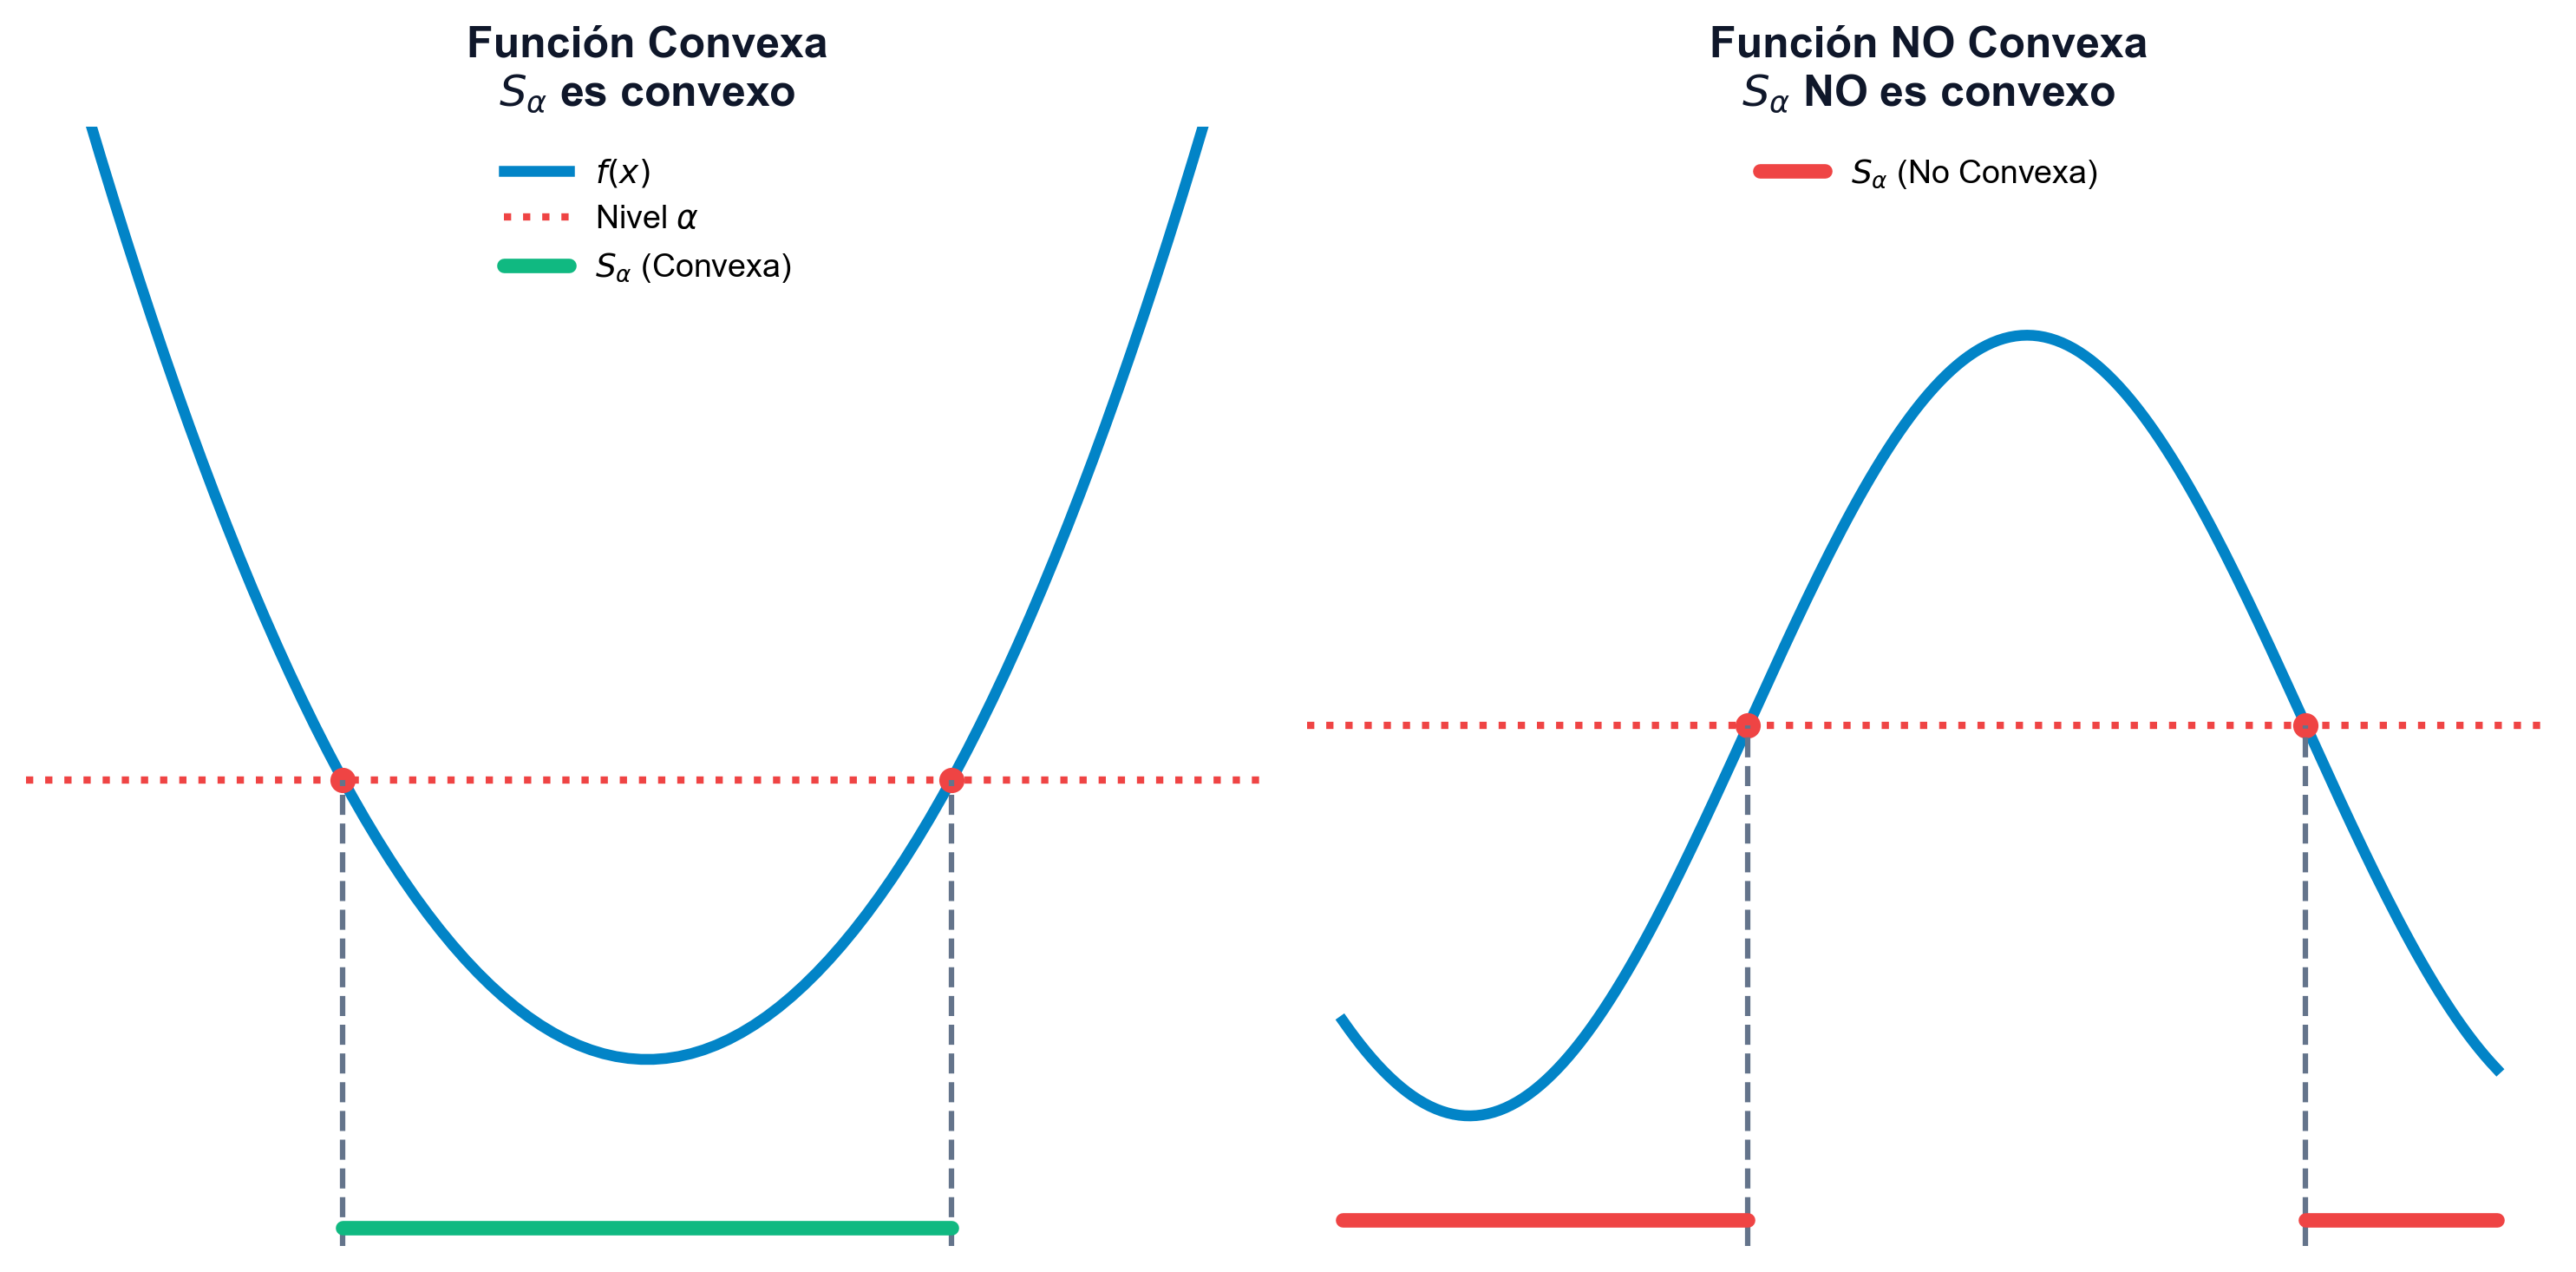
\includegraphics[width=0.85\linewidth,height=\textheight,keepaspectratio]{images/funciones_niveles_convexos.png}

}

\caption{\label{fig-funciones-niveles-convexos}Comparativa del conjunto
de nivel inferior \(\mathcal{S}_\alpha\): en una función convexa
(izquierda) es un intervalo continuo y por tanto convexo, mientras que
en una función no convexa (derecha) puede dar lugar a la unión de
intervalos disjuntos no convexos}

\end{figure}%

\begin{tcolorbox}[enhanced jigsaw, toprule=.15mm, opacitybacktitle=0.6, coltitle=black, colbacktitle=quarto-callout-warning-color!10!white, title=\textcolor{quarto-callout-warning-color}{\faExclamationTriangle}\hspace{0.5em}{Nota: El recíproco del teorema no es cierto}, arc=.35mm, rightrule=.15mm, toptitle=1mm, breakable, bottomtitle=1mm, titlerule=0mm, colback=white, opacityback=0, leftrule=.75mm, colframe=quarto-callout-warning-color-frame, left=2mm, bottomrule=.15mm]

El recíproco de este teorema no es cierto en general. Una función que
posee conjuntos de nivel inferior convexos no es necesariamente una
función convexa (esta propiedad estructural define la clase más general
de las funciones cuasi-convexas, como veremos más adelante).

\end{tcolorbox}

\subsection{Epigrafo e hipografo}\label{epigrafo-e-hipografo}

Para profundizar en el estudio analítico de las funciones convexas,
resulta muy provechoso vincular la estructura de la función con la
geometría de los conjuntos convexos. Esto se logra mediante el estudio
de las regiones geométricas que quedan por encima o por debajo de la
gráfica de la función. El \textbf{epigrafo} de una función \(f\)
(denotado por \(\text{epi } f\)) es el conjunto de puntos en el espacio
\(\mathbb{R}^{n+1}\) situados sobre o por encima de su gráfica:
\[ \text{epi } f = \{ (x, y) \in \mathcal{S} \times \mathbb{R} \mid y \ge f(x) \} \]
De forma complementaria, el \textbf{hipografo} (denotado por
\(\text{hyp } f\)) es el conjunto de puntos en el espacio
\(\mathbb{R}^{n+1}\) situados bajo o por debajo de la gráfica de la
función \(f\):
\[ \text{hyp } f = \{ (x, y) \in \mathcal{S} \times \mathbb{R} \mid y \le f(x) \} \]

La comparación tridimensional entre el epigrafo de una función convexa y
el hipografo de una cóncava se ilustra en la
Figura~\ref{fig-epigrafo-hipografo-3d}.

\begin{figure}

\centering{

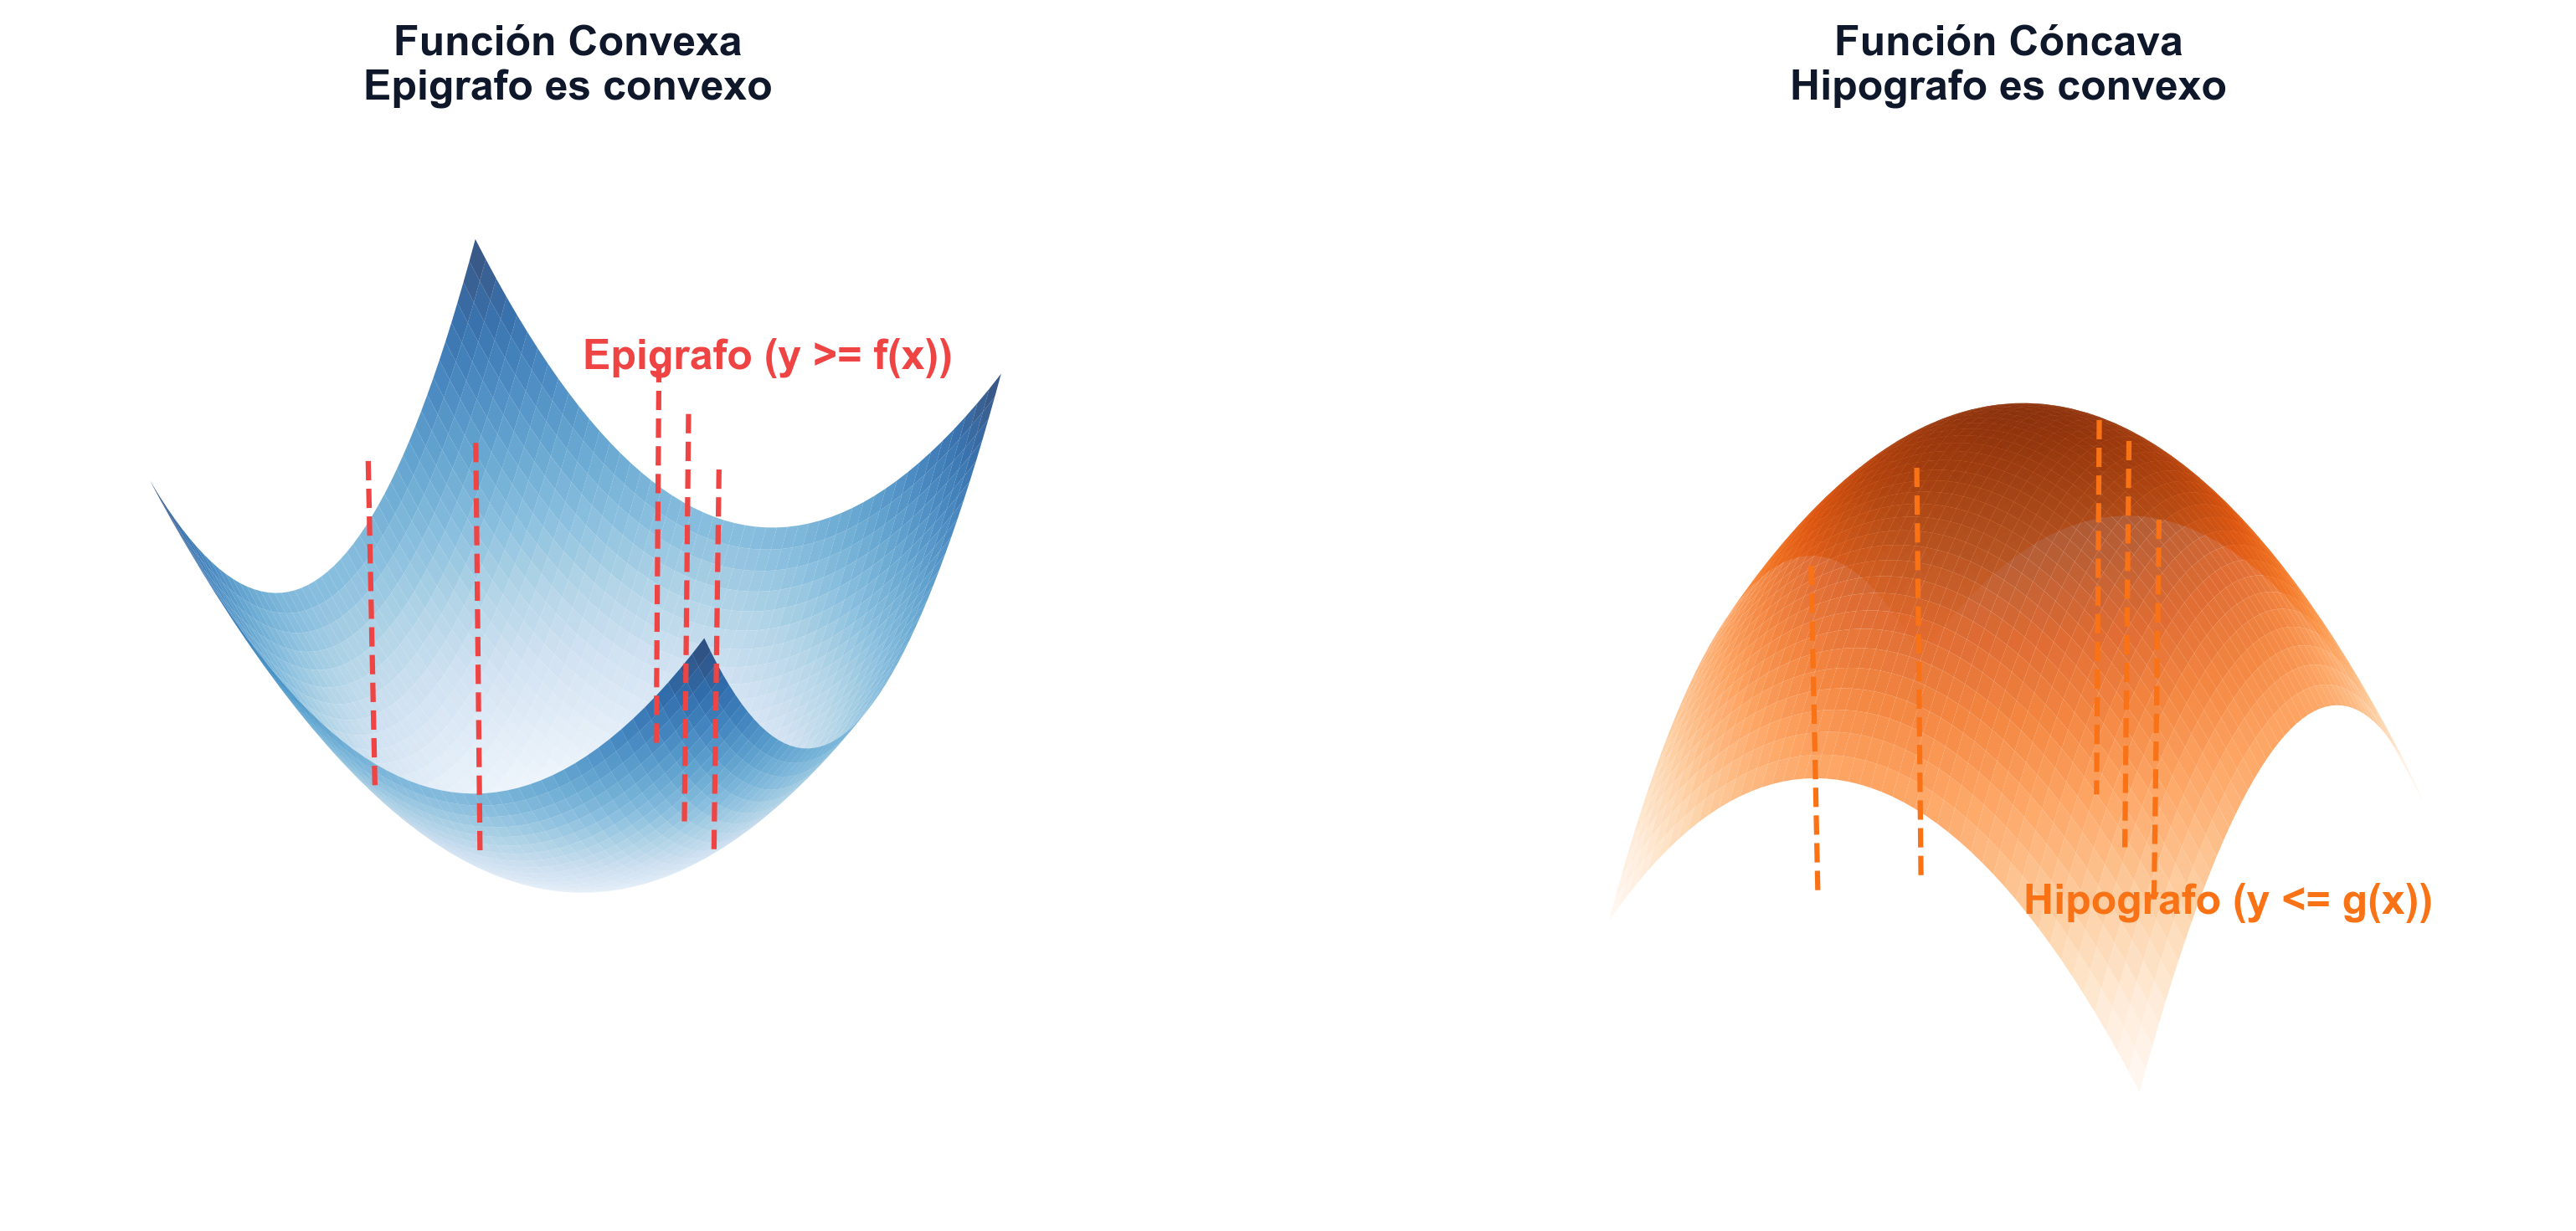
\includegraphics[width=0.9\linewidth,height=\textheight,keepaspectratio]{images/epigrafo_hipografo_3d.png}

}

\caption{\label{fig-epigrafo-hipografo-3d}Visualización tridimensional
comparativa del Epigrafo (región sombreada superior) para una función
convexa (izquierda) y del Hipografo (región sombreada inferior) para una
función cóncava (derecha)}

\end{figure}%

\begin{tcolorbox}[enhanced jigsaw, toprule=.15mm, opacitybacktitle=0.6, coltitle=black, colbacktitle=quarto-callout-important-color!10!white, title=\textcolor{quarto-callout-important-color}{\faExclamation}\hspace{0.5em}{Teorema: Relación entre epigrafo y convexidad}, arc=.35mm, rightrule=.15mm, toptitle=1mm, breakable, bottomtitle=1mm, titlerule=0mm, colback=white, opacityback=0, leftrule=.75mm, colframe=quarto-callout-important-color-frame, left=2mm, bottomrule=.15mm]

Una función \(f: \mathcal{S} \to \mathbb{R}\) es convexa si y solo si su
epigrafo \(\text{epi } f\) es un conjunto convexo en
\(\mathbb{R}^{n+1}\).

\emph{Demostración}: \((\Longrightarrow)\) Supongamos que \(f\) es
convexa. Sean \((x_1, y_1), (x_2, y_2) \in \text{epi } f\) y
\(\lambda \in (0, 1)\). Por definición de epigrafo, \(y_1 \ge f(x_1)\) y
\(y_2 \ge f(x_2)\). Evaluando la combinación lineal:
\[ \lambda y_1 + (1 - \lambda) y_2 \ge \lambda f(x_1) + (1 - \lambda) f(x_2) \ge f(\lambda x_1 + (1 - \lambda) x_2) \]
Como \(\mathcal{S}\) es convexo, el punto combinado pertenece a
\(\mathcal{S}\), y el par combinado pertenece a \(\text{epi } f\),
demostrando su convexidad.

\((\Longleftarrow)\) Supongamos que \(\text{epi } f\) es un conjunto
convexo. Sean \(x_1, x_2 \in \mathcal{S}\). Los puntos \((x_1, f(x_1))\)
y \((x_2, f(x_2))\) pertenecen a \(\text{epi } f\). Por convexidad del
epigrafo, para todo \(\lambda \in (0, 1)\):
\[ \lambda (x_1, f(x_1)) + (1 - \lambda)(x_2, f(x_2)) = (\lambda x_1 + (1 - \lambda) x_2, \lambda f(x_1) + (1 - \lambda) f(x_2)) \in \text{epi } f \]
Lo que implica directamente que
\(\lambda f(x_1) + (1 - \lambda) f(x_2) \ge f(\lambda x_1 + (1 - \lambda) x_2)\),
es decir, \(f\) es convexa. \(\blacksquare\)

\end{tcolorbox}

Esta equivalencia fundamental resulta sumamente potente, ya que permite
trasladar propiedades algebraicas complejas de las funciones al análisis
puramente geométrico de los conjuntos convexos. De manera completamente
análoga, la convexidad del hipografo caracteriza a las funciones
cóncavas: una función \(f\) es cóncava si y solo si su hipografo
\(\text{hyp } f\) es un conjunto convexo en \(\mathbb{R}^{n+1}\). De
este modo, la curvatura (hacia arriba o hacia abajo) de cualquier
función queda codificada de forma unívoca en la geometría del cuerpo que
delimita su gráfica.

Cuando trabajamos con funciones no diferenciables (es decir, aquellas
que presentan picos o codos en su gráfica), el gradiente clásico deja de
existir en ciertos puntos de interés. Para solventar este límite
analítico, generalizamos la noción de gradiente a través del concepto de
subgradiente.

Un vector \(\xi \in \mathbb{R}^n\) es un \textbf{subgradiente} de la
función convexa \(f\) en el punto \(x_0 \in \mathcal{S}\) si satisface
la desigualdad:
\[ f(x) \ge f(x_0) + \xi^T(x - x_0), \quad \forall x \in \mathcal{S} \]
Geométricamente, el subgradiente representa la pendiente de un
hiperplano de soporte que apoya a la función desde abajo en dicho punto.
El conjunto formado por todos los subgradientes de \(f\) en \(x_0\) se
denomina \textbf{subdiferencial} y se denota por \(\partial f(x_0)\).

\begin{figure}

\centering{

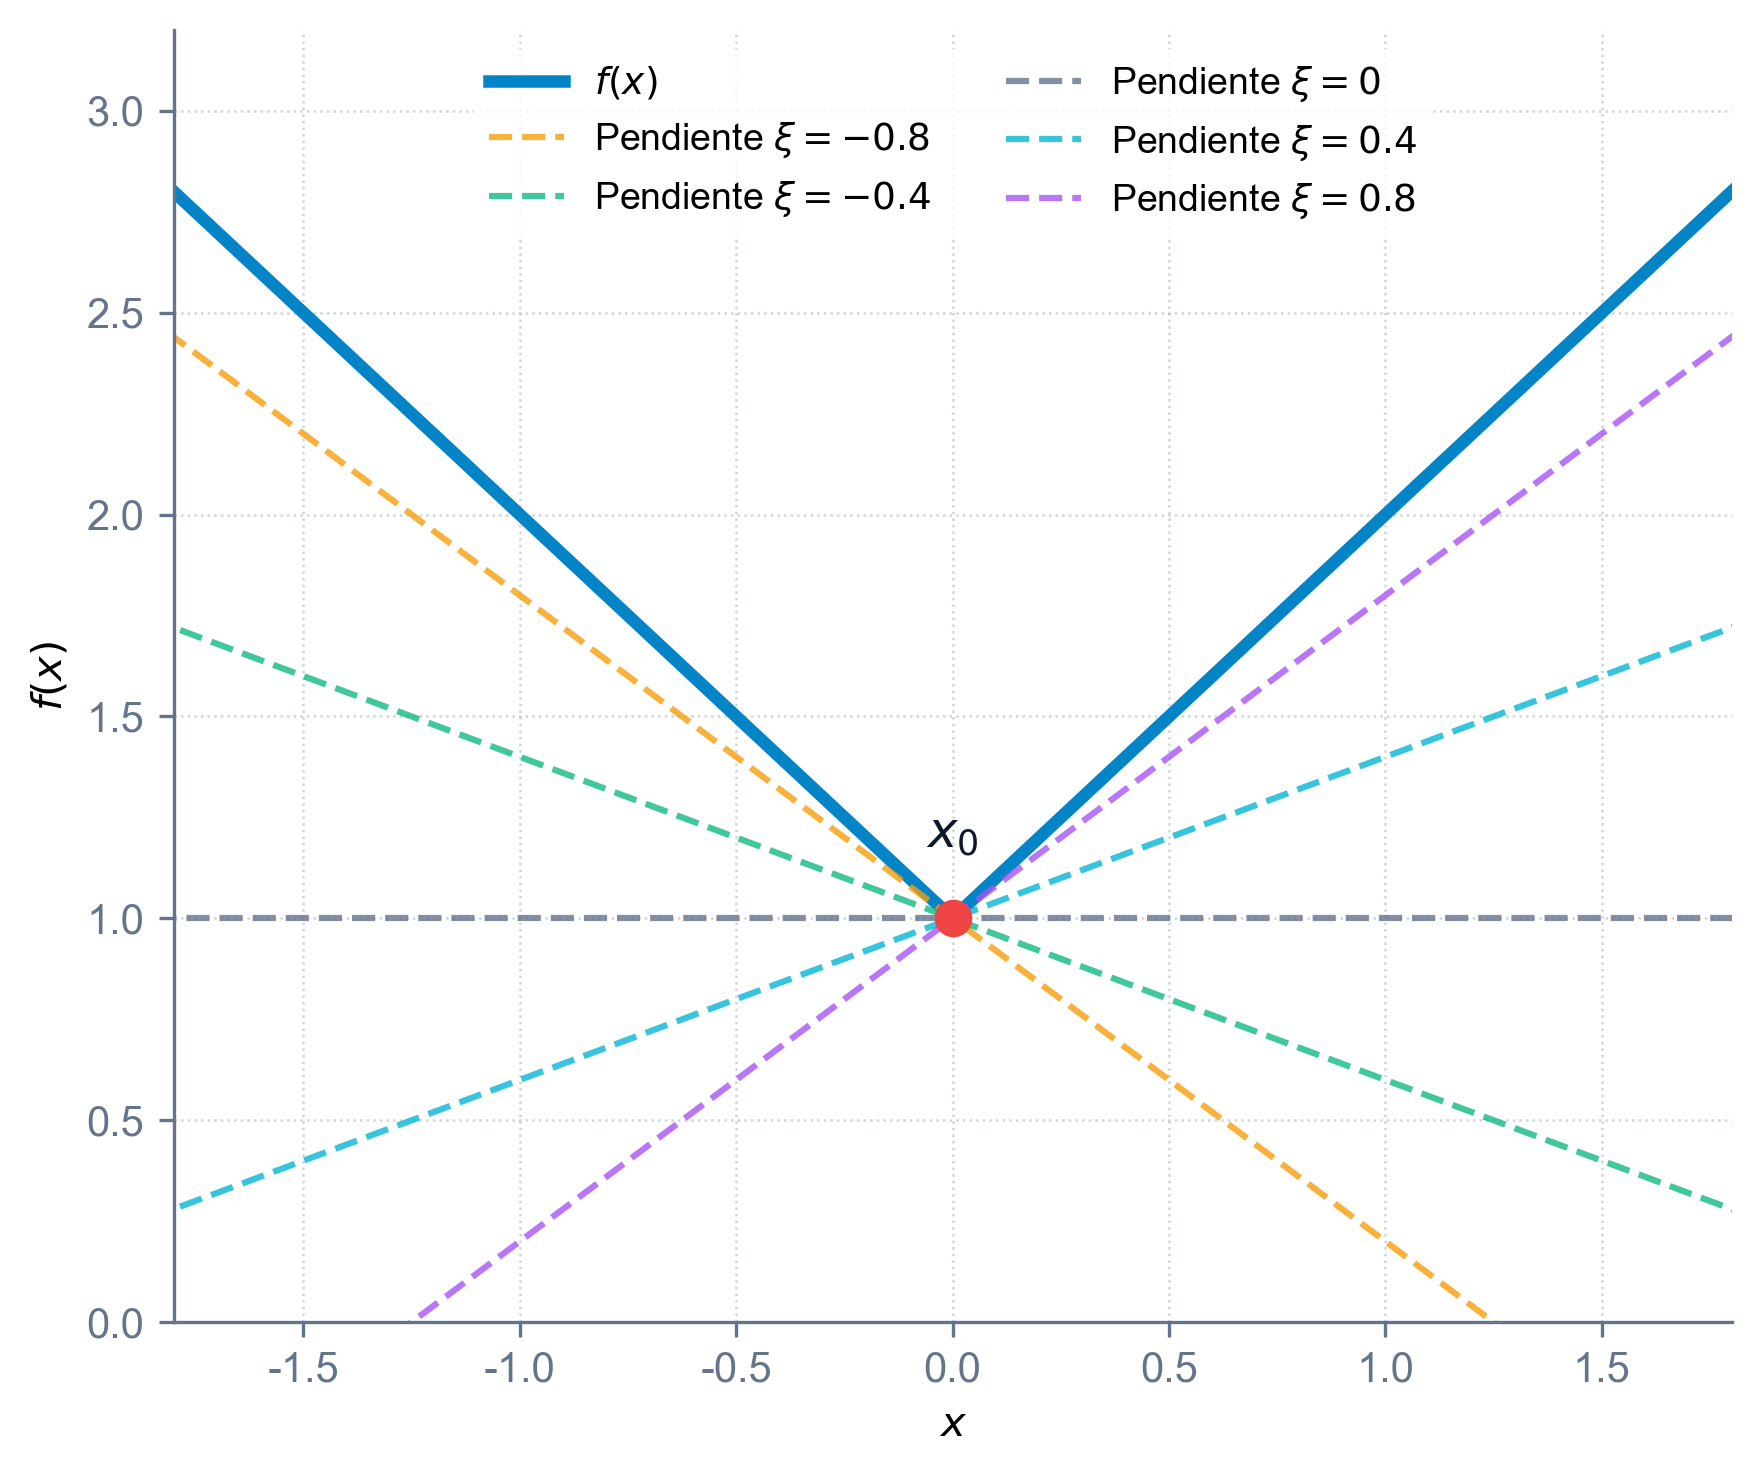
\includegraphics[width=0.6\linewidth,height=\textheight,keepaspectratio]{images/subgradientes_concepto.png}

}

\caption{\label{fig-subgradientes-concepto}Interpretación geométrica del
subgradiente y el subdiferencial para una función no diferenciable en
\(x_0\)}

\end{figure}%

El subdiferencial \(\partial f(x_0)\) es siempre un conjunto convexo y
cerrado, cuyas propiedades matemáticas se explotan rigurosamente en la
optimización no diferenciable (Rockafellar 1970; Boyd y Vandenberghe
2004). Si la función es diferenciable en un punto \(x_0\), el
subdiferencial contiene un único elemento que coincide exactamente con
el gradiente convencional: \(\partial f(x_0) = \{\nabla f(x_0)\}\).

\begin{tcolorbox}[enhanced jigsaw, toprule=.15mm, opacitybacktitle=0.6, coltitle=black, colbacktitle=quarto-callout-important-color!10!white, title=\textcolor{quarto-callout-important-color}{\faExclamation}\hspace{0.5em}{Teorema: Existencia del subgradiente (hiperplano soporte al epigrafo)}, arc=.35mm, rightrule=.15mm, toptitle=1mm, breakable, bottomtitle=1mm, titlerule=0mm, colback=white, opacityback=0, leftrule=.75mm, colframe=quarto-callout-important-color-frame, left=2mm, bottomrule=.15mm]

Sea \(f: \mathcal{S} \to \mathbb{R}\) una función convexa, con
\(\mathcal{S}\) un conjunto convexo no vacío de \(\mathbb{R}^n\). Para
cualquier punto interior \(x_0 \in \text{int }\mathcal{S}\), existe al
menos un subgradiente \(\xi \in \mathbb{R}^n\). Esto equivale a decir
que el hiperplano: \[ y = f(x_0) + \xi^T(x - x_0) \] es un hiperplano de
soporte para el epigrafo de \(f\), \(\text{epi } f\), en el punto
frontera \((x_0, f(x_0))\).

\emph{Demostración}: Por ser \(f\) convexa, su epigrafo \(\text{epi} f\)
es un conjunto convexo en \(\mathbb{R}^{n+1}\). Todo conjunto convexo
posee asociado un hiperplano de soporte en cada punto de su frontera. El
punto \((x_0, f(x_0))\) pertenece a la frontera de \(\text{epi } f\) (ya
que para cualquier \(\epsilon > 0\), el punto
\((x_0, f(x_0) - \epsilon) \notin \text{epi } f\) pero
\((x_0, f(x_0)) \in \text{epi } f\)).

Por consiguiente, existe un vector no nulo
\(\binom{\xi_0}{\mu} \in \mathbb{R}^{n+1}\) tal que:
\[ \xi_0^T(x - x_0) + \mu (y - f(x_0)) \le 0, \qquad \forall (x, y) \in \text{epi } f \]
En primer lugar, analizando \(y \to \infty\) para un \(x = x_0\) fijo,
para que la desigualdad se mantenga, el escalar \(\mu\) debe satisfacer
\(\mu \le 0\).

Demostremos ahora que \(\mu\) debe ser estrictamente negativo
(\(\mu < 0\)). Supongamos por contradicción que \(\mu = 0\). En tal
caso, la desigualdad anterior se reduce a:
\[ \xi_0^T(x - x_0) \le 0, \qquad \forall x \in \mathcal{S} \] Como
\(x_0 \in \text{int }\mathcal{S}\), existe una pequeña bola centrada en
\(x_0\) contenida en \(\mathcal{S}\), lo que permite tomar un punto de
la forma \(x = x_0 + \lambda \xi_0 \in \mathcal{S}\) para un
\(\lambda > 0\) suficientemente pequeño. Sustituyendo este punto:
\[ \lambda \xi_0^T \xi_0 \le 0 \implies \|\xi_0\|^2 \le 0 \implies \xi_0 = \mathbf{0} \]
Esto implica que el vector dual normal es
\((\xi_0, \mu) = (\mathbf{0}, 0)\), lo cual contradice la hipótesis de
que dicho vector es no nulo. Por tanto, \(\mu < 0\).

Definimos ahora el vector
\(\xi = \frac{\xi_0}{|\mu|} = \frac{\xi_0}{-\mu}\). Dividiendo la
inecuación original por \(|\mu| > 0\):
\[ \xi^T(x - x_0) - y + f(x_0) \le 0, \qquad \forall (x, y) \in \text{epi } f \]
Reordenando, obtenemos:
\[ y \ge f(x_0) + \xi^T(x - x_0), \qquad \forall (x, y) \in \text{epi } f \]
Evaluando esta desigualdad en el punto frontera de la gráfica
\(y = f(x)\), concluimos que:
\[ f(x) \ge f(x_0) + \xi^T(x - x_0), \qquad \forall x \in \mathcal{S} \]
lo que demuestra que \(\xi\) es un subgradiente de \(f\) en \(x_0\).
\(\blacksquare\)

\end{tcolorbox}

El teorema anterior garantiza que siempre es posible apoyar una función
convexa desde abajo mediante un hiperplano. Cuando la función posee una
curvatura estrictamente positiva (es decir, es estrictamente convexa),
este apoyo deja de ser plano en cualquier otro punto del dominio y el
hiperplano toca a la gráfica únicamente en el punto de tangencia, lo que
se formaliza a continuación.

\begin{tcolorbox}[enhanced jigsaw, toprule=.15mm, opacitybacktitle=0.6, coltitle=black, colbacktitle=quarto-callout-note-color!10!white, title=\textcolor{quarto-callout-note-color}{\faInfo}\hspace{0.5em}{Corolario: Caso de convexidad estricta}, arc=.35mm, rightrule=.15mm, toptitle=1mm, breakable, bottomtitle=1mm, titlerule=0mm, colback=white, opacityback=0, leftrule=.75mm, colframe=quarto-callout-note-color-frame, left=2mm, bottomrule=.15mm]

Si \(f: \mathcal{S} \to \mathbb{R}\) es estrictamente convexa, entonces
para cualquier \(x_0 \in \text{int }\mathcal{S}\) y cualquier
subgradiente \(\xi \in \partial f(x_0)\), se verifica la desigualdad
estricta:
\[ f(x) > f(x_0) + \xi^T(x - x_0), \quad \forall x \in \mathcal{S}, \ x \neq x_0 \]

\emph{Demostración}: Por el teorema de existencia, existe un
subgradiente \(\xi \in \partial f(x_0)\) tal que:
\[ f(x) \ge f(x_0) + \xi^T(x - x_0), \qquad \forall x \in \mathcal{S} \]
Supongamos por contradicción que existe un punto
\(x_1 \in \mathcal{S}\), \(x_1 \neq x_0\), donde se alcanza la igualdad:
\[ f(x_1) = f(x_0) + \xi^T(x_1 - x_0) \] Por la definición de convexidad
estricta de \(f\), para cualquier \(\lambda \in (0, 1)\):
\[ f(\lambda x_0 + (1-\lambda)x_1) < \lambda f(x_0) + (1-\lambda)f(x_1) \]
Sustituyendo el valor de \(f(x_1)\) en el miembro de la derecha:
\[ f(\lambda x_0 + (1-\lambda)x_1) < \lambda f(x_0) + (1-\lambda)[f(x_0) + \xi^T(x_1 - x_0)] = f(x_0) + (1-\lambda)\xi^T(x_1 - x_0) \]
Por otra parte, evaluando la inecuación del subgradiente original en el
punto \(x = \lambda x_0 + (1-\lambda)x_1\):
\[ f(\lambda x_0 + (1-\lambda)x_1) \ge f(x_0) + \xi^T[\lambda x_0 + (1-\lambda)x_1 - x_0] = f(x_0) + (1-\lambda)\xi^T(x_1 - x_0) \]
Las dos desigualdades anteriores son contradictorias, lo que concluye
que no puede darse la igualdad para ningún punto \(x_1 \neq x_0\).
\(\blacksquare\)

\end{tcolorbox}

Hasta el momento hemos deducido que la convexidad implica la existencia
de subgradientes que acotan inferiormente a la función. Un resultado de
enorme relevancia práctica es que esta relación es bidireccional: la
existencia de un vector de soporte inferior en cada punto del dominio es
suficiente para asegurar que la función es convexa, lo cual permite
verificar la convexidad de forma local.

\begin{tcolorbox}[enhanced jigsaw, toprule=.15mm, opacitybacktitle=0.6, coltitle=black, colbacktitle=quarto-callout-important-color!10!white, title=\textcolor{quarto-callout-important-color}{\faExclamation}\hspace{0.5em}{Teorema: Suficiencia de la caracterización por subgradientes}, arc=.35mm, rightrule=.15mm, toptitle=1mm, breakable, bottomtitle=1mm, titlerule=0mm, colback=white, opacityback=0, leftrule=.75mm, colframe=quarto-callout-important-color-frame, left=2mm, bottomrule=.15mm]

Sea \(\mathcal{S}\) un conjunto convexo abierto no vacío de
\(\mathbb{R}^n\) y sea \(f: \mathcal{S} \to \mathbb{R}\) una función. Si
para cada punto \(x_0 \in \mathcal{S}\) existe un vector
\(\xi \in \mathbb{R}^n\) tal que:
\[ f(x) \ge f(x_0) + \xi^T(x - x_0), \quad \forall x \in \mathcal{S} \]
entonces la función \(f\) es convexa en \(\mathcal{S}\).

\emph{Demostración}: Sean \(x_1, x_2 \in \mathcal{S}\) y
\(\lambda \in (0, 1)\). Definimos el punto intermedio
\(x_0 = \lambda x_1 + (1-\lambda)x_2\). Como \(\mathcal{S}\) es convexo
y abierto, \(x_0 \in \mathcal{S}\). Por hipótesis, existe un
subgradiente \(\xi\) en \(x_0\), tal que:
\[ f(x) \ge f(x_0) + \xi^T(x - x_0), \quad \forall x \in \mathcal{S} \]
Evaluando esta desigualdad en \(x = x_1\) y multiplicándola por
\(\lambda\):
\[ \lambda f(x_1) \ge \lambda f(x_0) + \lambda \xi^T(x_1 - x_0) \]
Evaluando la desigualdad en \(x = x_2\) y multiplicándola por
\((1-\lambda)\):
\[ (1-\lambda) f(x_2) \ge (1-\lambda) f(x_0) + (1-\lambda) \xi^T(x_2 - x_0) \]
Sumando ambas expresiones:
\[ \lambda f(x_1) + (1-\lambda) f(x_2) \ge [\lambda + (1-\lambda)]f(x_0) + \xi^T \left[ \lambda (x_1 - x_0) + (1-\lambda)(x_2 - x_0) \right] \]
Analizando el término dentro del producto escalar:
\[ \lambda(x_1 - x_0) + (1-\lambda)(x_2 - x_0) = \lambda x_1 + (1-\lambda)x_2 - [\lambda + (1-\lambda)]x_0 = x_0 - x_0 = 0 \]
Por tanto, el producto escalar se anula y obtenemos:
\[ \lambda f(x_1) + (1-\lambda) f(x_2) \ge f(x_0) = f(\lambda x_1 + (1-\lambda)x_2) \]
lo que demuestra que \(f\) es convexa. \(\blacksquare\)

\end{tcolorbox}

Para poder aplicar estas caracterizaciones en la resolución de problemas
reales, es necesario disponer de un álgebra que permita calcular el
subdiferencial de funciones complejas construidas a partir de funciones
más simples. Las siguientes propiedades establecen las reglas operativas
básicas del subdiferencial, de forma homóloga al cálculo diferencial
clásico.

\begin{tcolorbox}[enhanced jigsaw, toprule=.15mm, opacitybacktitle=0.6, coltitle=black, colbacktitle=quarto-callout-note-color!10!white, title=\textcolor{quarto-callout-note-color}{\faInfo}\hspace{0.5em}{Propiedades y cálculo del subdiferencial}, arc=.35mm, rightrule=.15mm, toptitle=1mm, breakable, bottomtitle=1mm, titlerule=0mm, colback=white, opacityback=0, leftrule=.75mm, colframe=quarto-callout-note-color-frame, left=2mm, bottomrule=.15mm]

El cálculo con subgradientes sigue reglas análogas al cálculo
diferencial estándar:

\begin{enumerate}
\def\labelenumi{\arabic{enumi}.}
\tightlist
\item
  \textbf{Regla de la Suma}: Si \(f_1, f_2\) son funciones convexas, el
  subdiferencial de su suma cumple:
  \[ \partial (f_1(x) + f_2(x)) = \partial f_1(x) \oplus \partial f_2(x) \]
\item
  \textbf{Multiplicación Escalar}: Para cualquier constante
  \(\alpha \ge 0\): \[ \partial (\alpha f(x)) = \alpha \partial f(x) \]
\item
  \textbf{Máximo de Funciones}: Si \(f(x) = \max \{f_1(x), f_2(x)\}\)
  con \(f_1, f_2\) convexas:
  \[ \partial f(x) = \mathcal{H}(\cup_{i \in \mathcal{I}(x)} \partial f_i(x)) \]
  donde \(\mathcal{I}(x)\) es el conjunto de índices de las funciones
  que alcanzan el máximo en el punto \(x\).
\end{enumerate}

\end{tcolorbox}

Para ilustrar de forma práctica la aplicación de las reglas algebraicas
del subdiferencial y el papel geométrico del subgradiente (como plano o
recta soporte inferior), a continuación se exponen detalladamente dos
casos de estudio de referencia. El primero analiza de manera exhaustiva
el comportamiento de una función valor absoluto no suave en una
dimensión, mostrando cómo el subdiferencial se ensancha en los puntos de
no diferenciabilidad. El segundo caso extiende esta noción a una función
multivariable diferenciable en dos dimensiones, calculando la ecuación
explícita del plano soporte en \(\mathbb{R}^3\).

\begin{tcolorbox}[enhanced jigsaw, toprule=.15mm, opacitybacktitle=0.6, coltitle=black, colbacktitle=quarto-callout-tip-color!10!white, title=\textcolor{quarto-callout-tip-color}{\faLightbulb}\hspace{0.5em}{Ejemplos: Cálculo y aplicación del subdiferencial en 1D y 2D}, arc=.35mm, rightrule=.15mm, toptitle=1mm, breakable, bottomtitle=1mm, titlerule=0mm, colback=white, opacityback=0, leftrule=.75mm, colframe=quarto-callout-tip-color-frame, left=2mm, bottomrule=.15mm]

\textbf{Caso 1D: Función no diferenciable definida por tramos}

Consideremos una función convexa clásica definida por tramos:
\[ f(x) = \max \{ |x| - 4, \ (x - 2)^2 - 4 \} \] Esta función puede
simplificarse en distintas regiones analizando cuál de las dos curvas
domina en cada intervalo (dado que la parábola y la función valor
absoluto se cruzan en \(x = 1\) y \(x = 4\)):
\[ f(x) = \begin{cases} x - 4 & \text{si } 1 \le x \le 4 \\ (x - 2)^2 - 4 & \text{en otro caso} \end{cases} \]

Analicemos su subdiferencial \(\partial f(x_0)\) en diferentes puntos de
la recta real:

En un \textbf{punto diferenciable en el tramo lineal} (por ejemplo,
\(x_0 = 2\)), la función es puramente lineal y coincide con la recta
\(x - 4\). Su derivada clásica es constante e igual a \(f'(2) = 1\). Al
ser diferenciable, el subdiferencial consta de un único vector:
\[ \partial f(2) = \{1\} \] La recta tangente soporte es
\(y = -2 + 1(x - 2) = x - 4\).

En un \textbf{punto diferenciable en el tramo cuadrático} (por ejemplo,
\(x_0 = 5\)), para valores superiores a 4, la función coincide con la
parábola \((x-2)^2 - 4\). Su derivada clásica en este punto es
\(f'(5) = 2(5 - 2) = 6\). Por tanto, el subdiferencial contiene
únicamente a esta pendiente: \[ \partial f(5) = \{6\} \] La recta
tangente soporte es \(y = 5 + 6(x - 5) = 6x - 25\).

En un \textbf{punto singular o codo} (en \(x_0 = 1\)), confluyen la
parábola (por la izquierda) y la recta (por la derecha). La derivada
lateral izquierda (cuadrática) es \(f'_{-}(1) = 2(1-2) = -2\), y la
derivada lateral derecha (lineal) es \(f'_{+}(1) = 1\). El
subdiferencial en este codo está formado por toda la familia de
pendientes intermedias (es decir, la combinación convexa de las
derivadas laterales): \[ \partial f(1) = [-2, 1] \] Cualquier línea que
pase por \((1, -3)\) con pendiente \(\xi \in [-2, 1]\) apoyará a la
función desde abajo (como la línea horizontal de pendiente \(\xi = 0\)).

En un \textbf{punto singular o codo} (en \(x_0 = 4\)), de manera
análoga, la derivada lateral izquierda (lineal) es \(f'_{-}(4) = 1\), y
la derivada lateral derecha (cuadrática) es \(f'_{+}(4) = 2(4-2) = 4\).
El subdiferencial es el intervalo: \[ \partial f(4) = [1, 4] \]

\begin{figure}[H]

\centering{

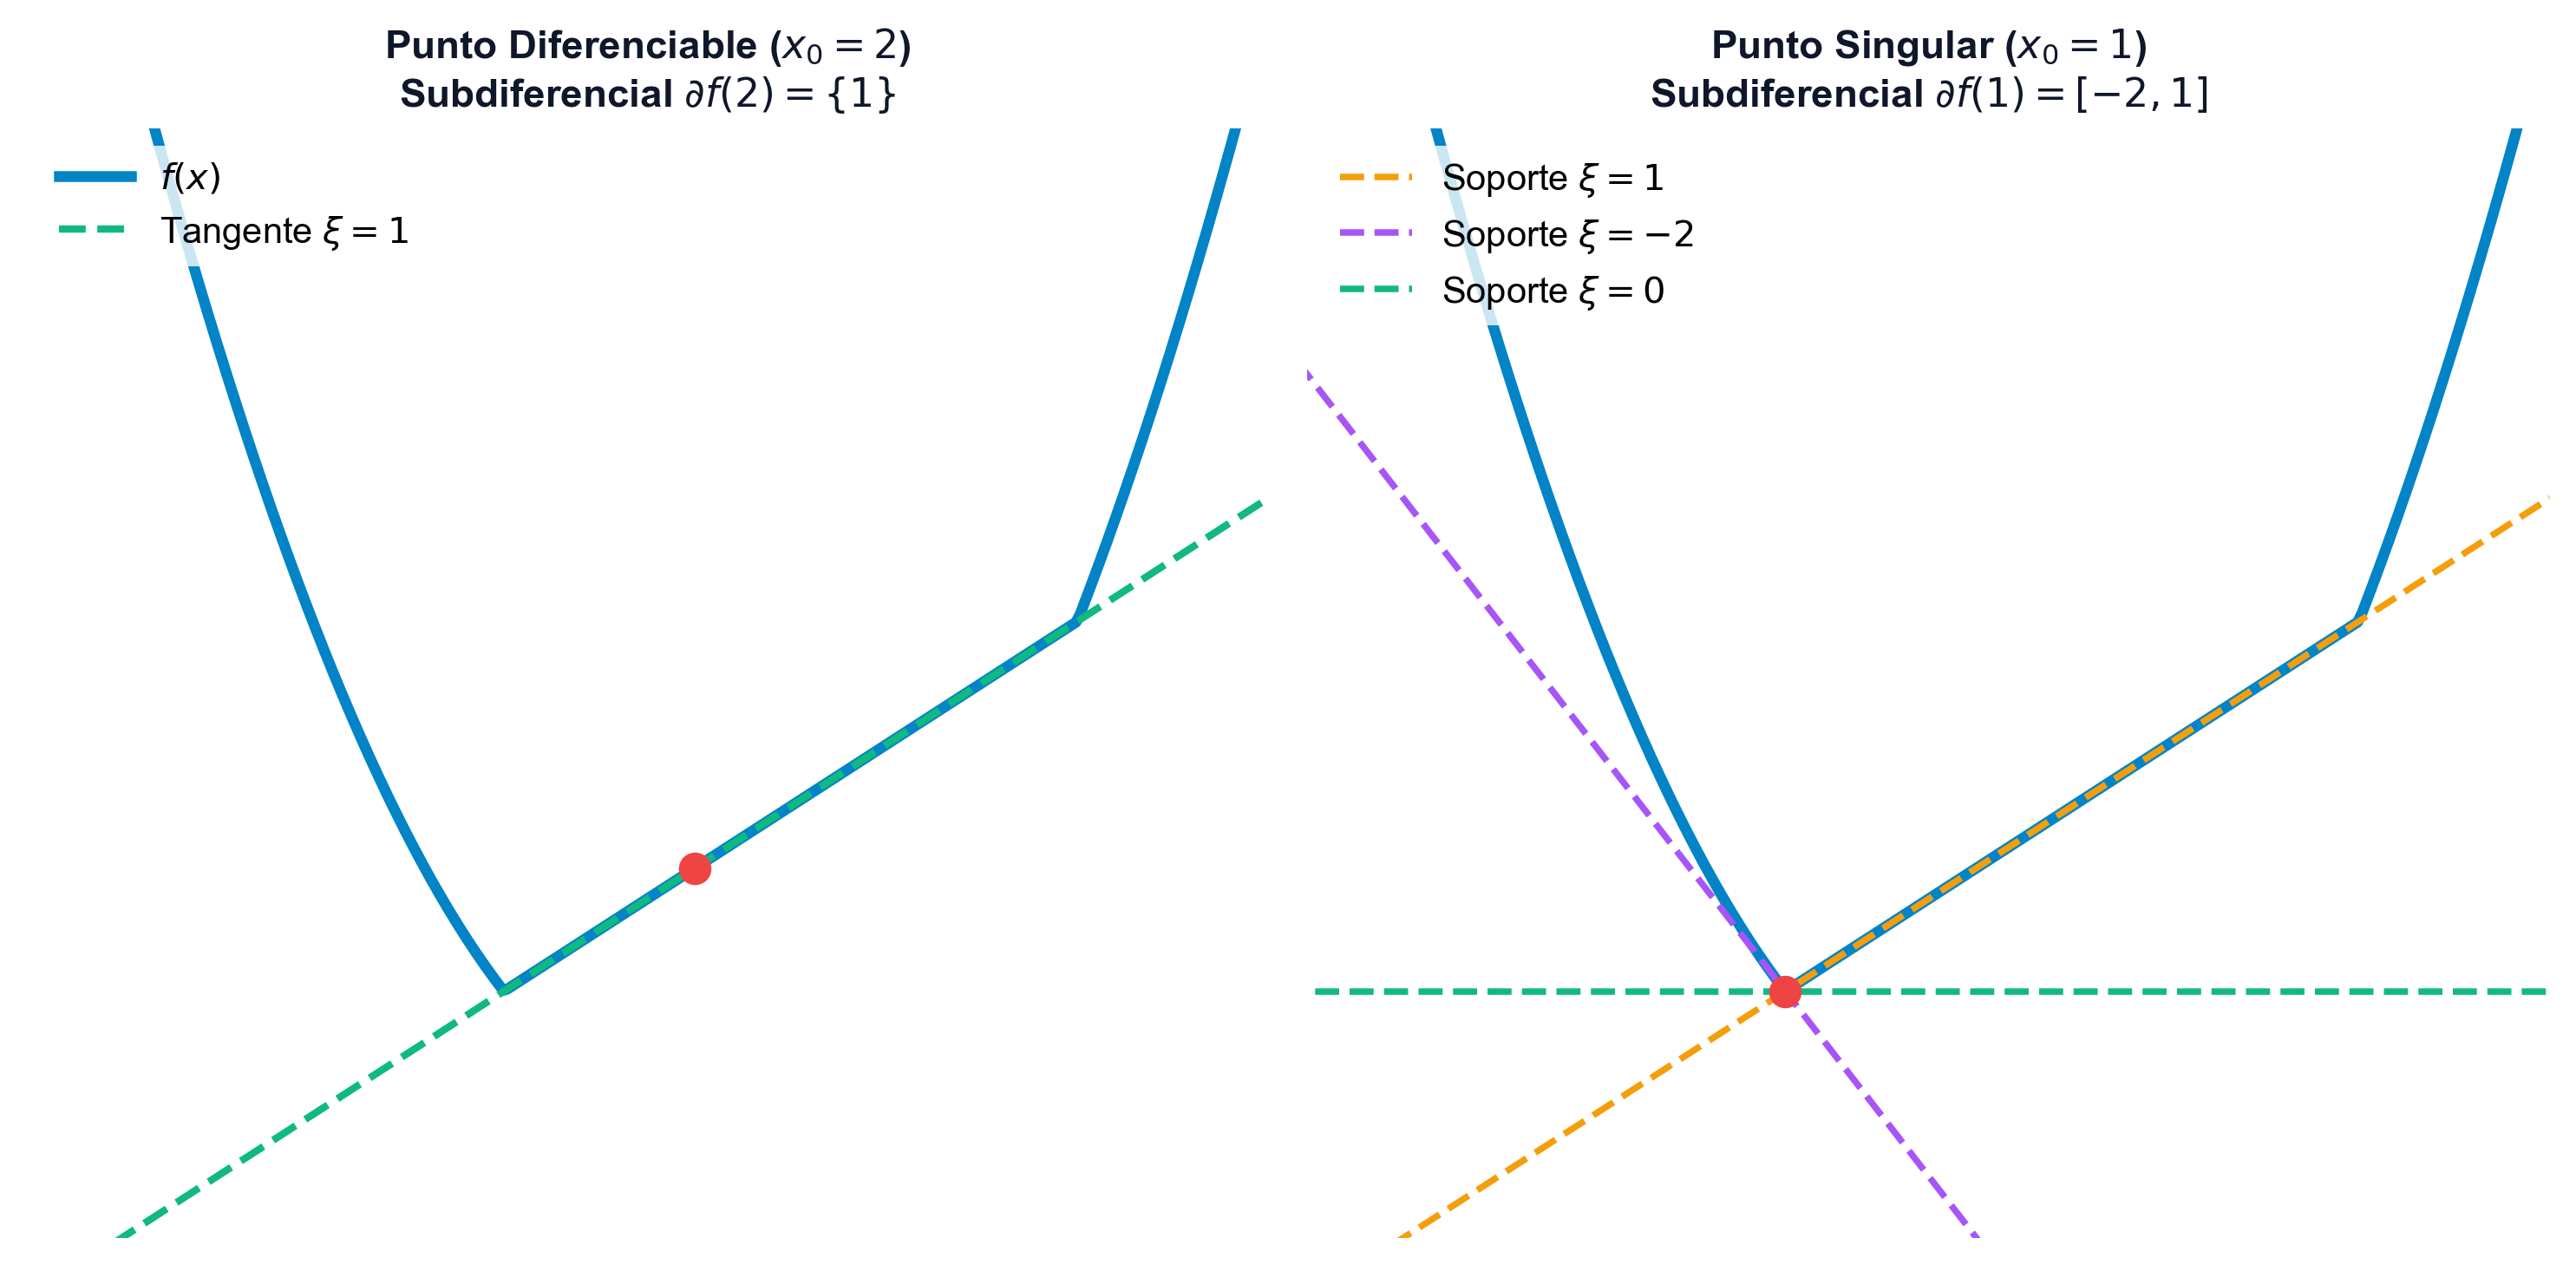
\includegraphics[width=0.85\linewidth,height=\textheight,keepaspectratio]{images/subgradientes_ejemplo_completo.png}

}

\caption{\label{fig-subgradientes-ejemplo-completo}Visualización del
subdiferencial de una función en un punto donde es diferenciable
(izquierda, tangente única) frente a un punto singular de codo (derecha,
múltiples pendientes de soporte en el intervalo de subdiferencial)}

\end{figure}%

\textbf{Caso 2D: Función cuadrática diferenciable y plano soporte}

Para ilustrar cómo se comporta el subdiferencial y el hiperplano soporte
en una dimensión superior, consideremos la función cuadrática
diferenciable \(f: \mathbb{R}^2 \to \mathbb{R}\) definida por:
\[ f(x, y) = 8x^2 + 3xy + 7y^2 - 25x + 31y - 29 \]

Calculamos su subdiferencial en el punto \(x_0 = (10, 10)\). Dado que
\(f\) es diferenciable en todo su dominio, el subdiferencial es unitario
y contiene únicamente al gradiente:
\[ \partial f(10, 10) = \{ \nabla f(10, 10) \} \]

Calculando las derivadas parciales de primer orden:
\[ \frac{\partial f}{\partial x} = 16x + 3y - 25 \implies \frac{\partial f}{\partial x}(10, 10) = 160 + 30 - 25 = 165 \]
\[ \frac{\partial f}{\partial y} = 3x + 14y + 31 \implies \frac{\partial f}{\partial y}(10, 10) = 30 + 140 + 31 = 201 \]

El valor de la función en dicho punto es:
\[ f(10, 10) = 8(100) + 3(100) + 7(100) - 250 + 310 - 29 = 1831 \]

Por tanto, el único subgradiente de la función en \((10, 10)\) es el
vector gradiente \(\xi = \nabla f(10, 10) = (165, 201)^T\). El plano
soporte tangente en 3D que acota inferiormente a la función viene
definido por el hiperplano: \[ z = 1831 + 165(x - 10) + 201(y - 10) \]

De acuerdo con el teorema de existencia, la convexidad de \(f\)
garantiza de forma global que:
\[ 8x^2 + 3xy + 7y^2 - 25x + 31y - 29 \ge 1831 + 165(x - 10) + 201(y - 10), \quad \forall (x, y) \in \mathbb{R}^2 \]

\begin{figure}[H]

\centering{

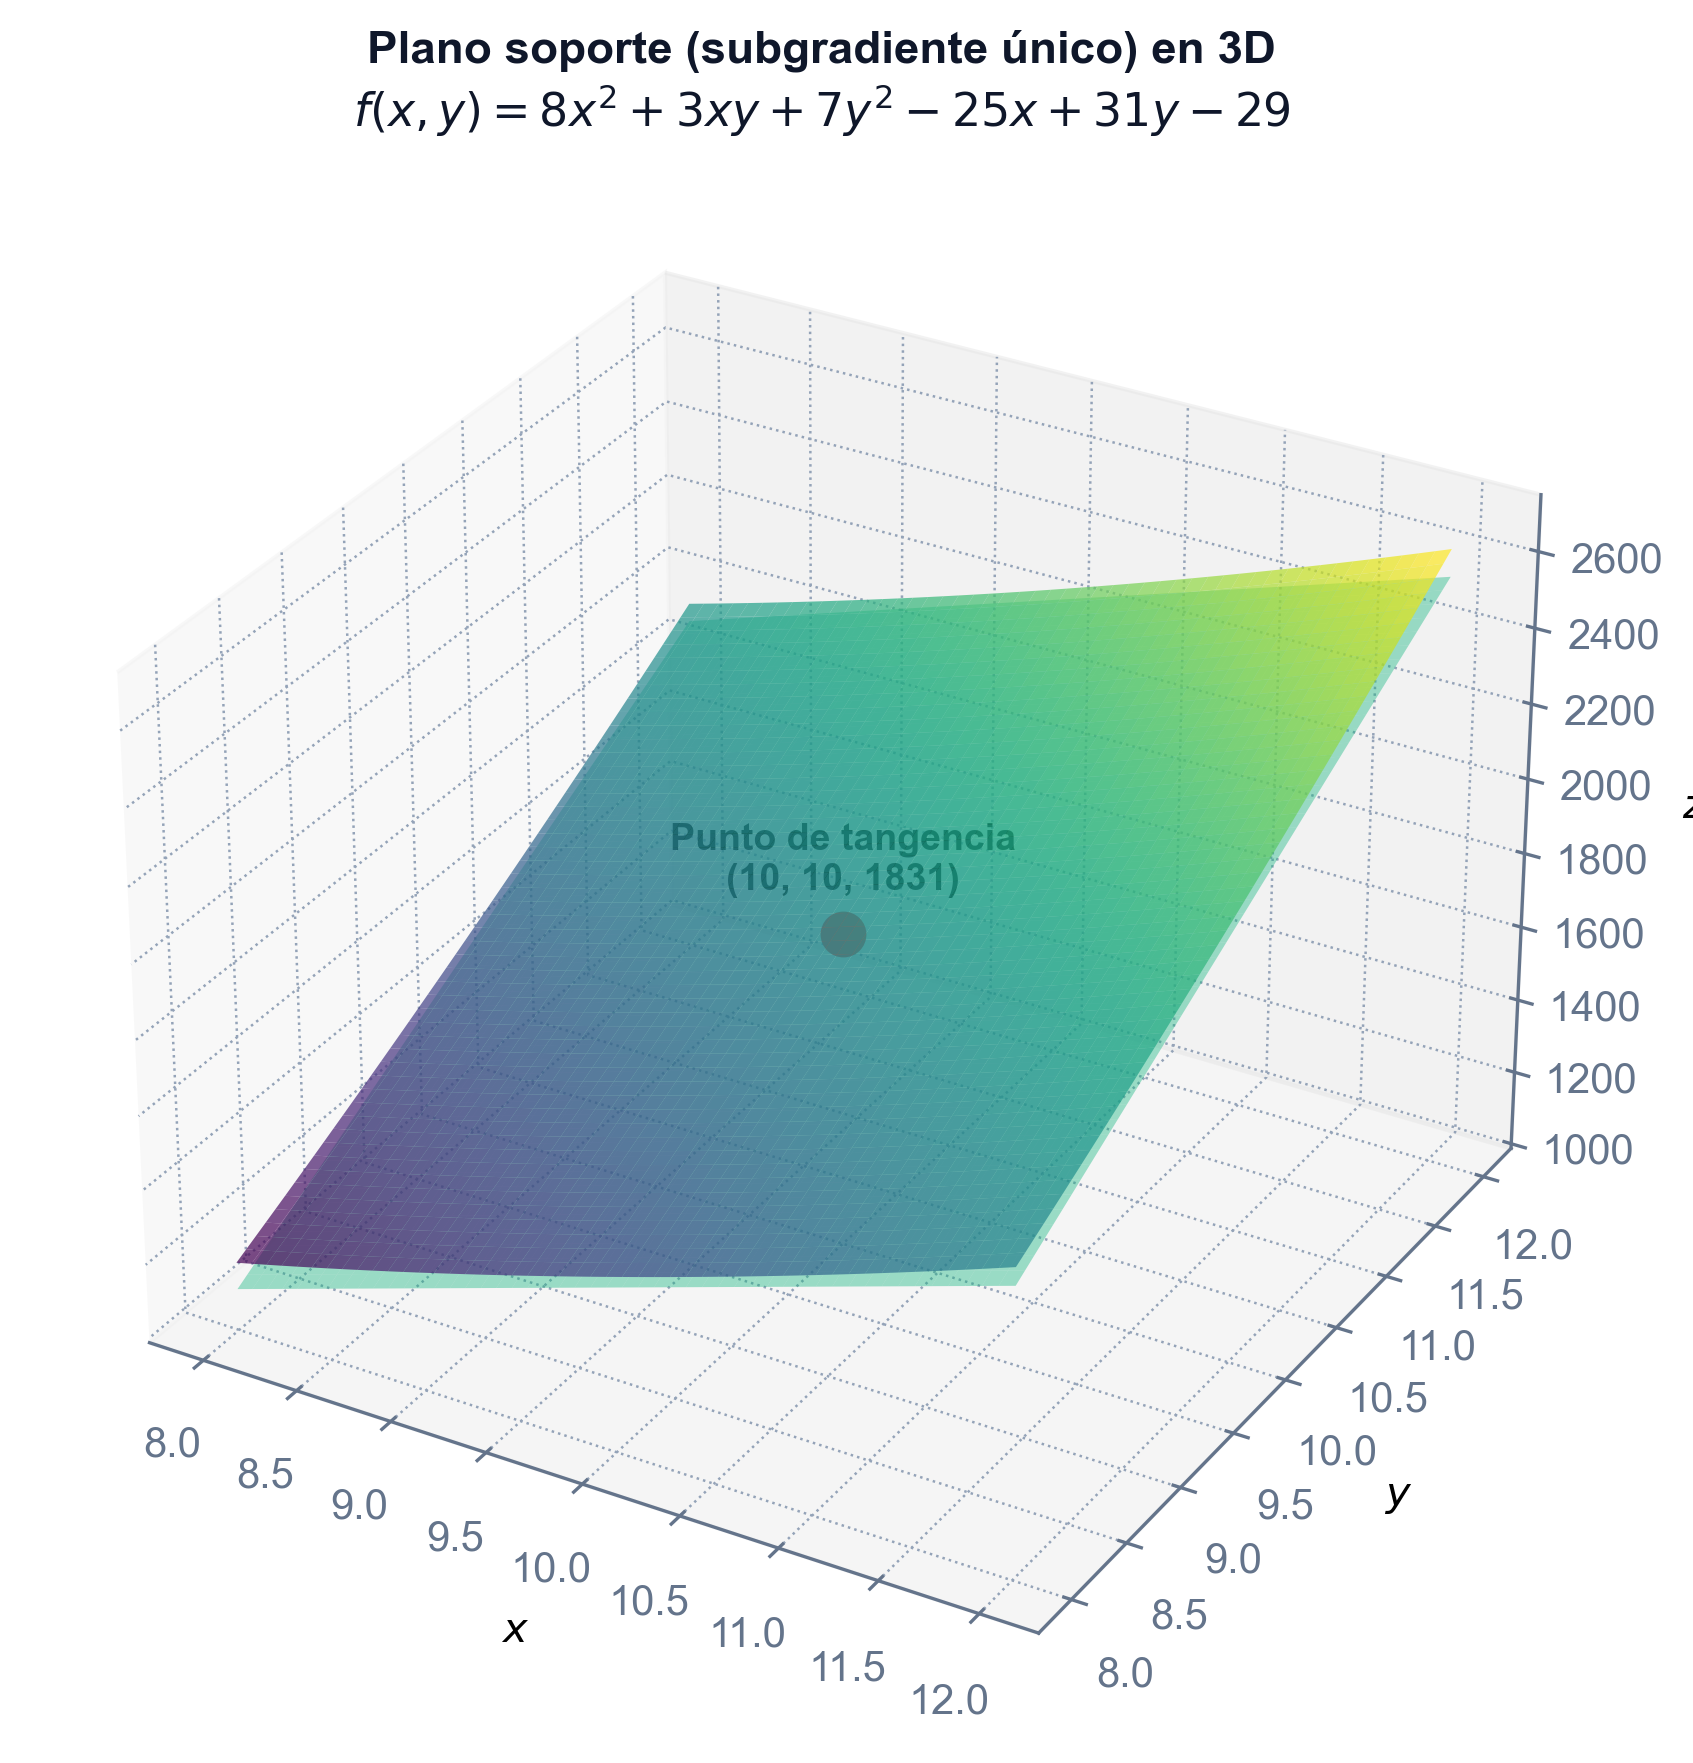
\includegraphics[width=0.7\linewidth,height=\textheight,keepaspectratio]{images/subgradiente_3d.png}

}

\caption{\label{fig-subgradiente-3d}Plano tangente de soporte inferior
en 3D para una función cuadrática diferenciable convexa en el punto de
tangencia (10, 10, 1831)}

\end{figure}%

\end{tcolorbox}

\section{Caracterización de funciones convexas
diferenciables}\label{caracterizaciuxf3n-de-funciones-convexas-diferenciables}

Aunque las definiciones geométricas basadas en epigrafos o combinaciones
lineales de puntos son conceptualmente intuitivas, en la práctica
matemática y algorítmica resulta muy costoso verificar la convexidad de
una función directamente a partir de ellas. Cuando la función posee
propiedades de suavidad, es decir, es diferenciable (una o dos veces),
es posible explotar la información local proporcionada por sus derivadas
para establecer criterios de convexidad globales más sencillos de
evaluar. En esta sección se abordan los resultados fundamentales que
conectan el gradiente y la matriz hessiana con la geometría convexa.

\begin{tcolorbox}[enhanced jigsaw, toprule=.15mm, opacitybacktitle=0.6, coltitle=black, colbacktitle=quarto-callout-important-color!10!white, title=\textcolor{quarto-callout-important-color}{\faExclamation}\hspace{0.5em}{Teorema: Caracterización de primer orden para funciones diferenciables}, arc=.35mm, rightrule=.15mm, toptitle=1mm, breakable, bottomtitle=1mm, titlerule=0mm, colback=white, opacityback=0, leftrule=.75mm, colframe=quarto-callout-important-color-frame, left=2mm, bottomrule=.15mm]

Sea \(f: \mathcal{S} \to \mathbb{R}\) una función diferenciable en un
conjunto convexo y abierto \(\mathcal{S}\).

\begin{enumerate}
\def\labelenumi{\arabic{enumi}.}
\tightlist
\item
  \(f\) es convexa si y solo si:
  \[ f(x) \ge f(x_0) + \nabla f(x_0)^T (x - x_0), \quad \forall x, x_0 \in \mathcal{S} \]
\item
  \(f\) es estrictamente convexa si y solo si:
  \[ f(x) > f(x_0) + \nabla f(x_0)^T (x - x_0), \quad \forall x, x_0 \in \mathcal{S} \text{ con } x \neq x_0 \]
\end{enumerate}

\end{tcolorbox}

\emph{Significado geométrico}: La aproximación lineal de primer orden
(plano tangente en cualquier punto \(x_0\)) es un estimador inferior
global de la función. Es decir, la gráfica de la función se apoya en su
totalidad sobre el plano tangente.

La caracterización de primer orden anterior establece que una función
convexa siempre crece más rápido (o igual) que su aproximación lineal
tangente. Esta propiedad tiene una consecuencia directa sobre el
comportamiento de sus gradientes: a medida que nos desplazamos por el
dominio, el gradiente debe variar de forma que siempre apunte en
direcciones de crecimiento. Esto da lugar a la noción de monotonía del
operador gradiente, lo que formaliza algebraicamente la idea de que la
pendiente de la función no decrece en ninguna dirección.

\begin{tcolorbox}[enhanced jigsaw, toprule=.15mm, opacitybacktitle=0.6, coltitle=black, colbacktitle=quarto-callout-important-color!10!white, title=\textcolor{quarto-callout-important-color}{\faExclamation}\hspace{0.5em}{Teorema: Monotonía del gradiente}, arc=.35mm, rightrule=.15mm, toptitle=1mm, breakable, bottomtitle=1mm, titlerule=0mm, colback=white, opacityback=0, leftrule=.75mm, colframe=quarto-callout-important-color-frame, left=2mm, bottomrule=.15mm]

Una función diferenciable \(f\) es convexa en un conjunto convexo
abierto \(\mathcal{S}\) si y solo si su gradiente es un operador
monótono:
\[ (\nabla f(x_2) - \nabla f(x_1))^T(x_2 - x_1) \ge 0, \quad \forall x_1, x_2 \in \mathcal{S} \]

\emph{Demostración}: \((\Longrightarrow)\) Si \(f\) es convexa, por la
caracterización de primer orden se cumplen simultáneamente:
\[ f(x_1) \ge f(x_2) + \nabla f(x_2)^T (x_1 - x_2) \]
\[ f(x_2) \ge f(x_1) + \nabla f(x_1)^T (x_2 - x_1) \] Sumando ambas
inecuaciones miembro a miembro:
\[ f(x_1) + f(x_2) \ge f(x_2) + f(x_1) + \nabla f(x_2)^T(x_1 - x_2) + \nabla f(x_1)^T(x_2 - x_1) \]
Cancelando términos comunes y reordenando:
\[ 0 \ge (\nabla f(x_1) - \nabla f(x_2))^T (x_2 - x_1) \implies (\nabla f(x_2) - \nabla f(x_1))^T(x_2 - x_1) \ge 0 \]
\((\Longleftarrow)\) Se demuestra de manera análoga aplicando el teorema
del valor medio. \(\blacksquare\)

\end{tcolorbox}

El análisis del gradiente de primer orden nos proporciona una visión del
comportamiento de las pendientes de la función. Sin embargo, para
funciones dos veces diferenciables, podemos refinar este análisis
estudiando la tasa de variación de las pendientes, es decir, la
curvatura de la función. Esto se logra mediante el estudio de la matriz
hessiana, cuyas propiedades de definición y semidefinición positiva
determinan de forma local si la curvatura es siempre ascendente
(convexa), garantizando la convexidad de manera global.

\begin{tcolorbox}[enhanced jigsaw, toprule=.15mm, opacitybacktitle=0.6, coltitle=black, colbacktitle=quarto-callout-important-color!10!white, title=\textcolor{quarto-callout-important-color}{\faExclamation}\hspace{0.5em}{Teorema: Caracterización de segundo orden}, arc=.35mm, rightrule=.15mm, toptitle=1mm, breakable, bottomtitle=1mm, titlerule=0mm, colback=white, opacityback=0, leftrule=.75mm, colframe=quarto-callout-important-color-frame, left=2mm, bottomrule=.15mm]

Sea \(f: \mathcal{S} \to \mathbb{R}\) una función dos veces
diferenciable en un conjunto convexo abierto \(\mathcal{S}\).

\begin{enumerate}
\def\labelenumi{\arabic{enumi}.}
\tightlist
\item
  \(f\) es convexa si y solo si su matriz hessiana es semidefinida
  positiva en todo punto de \(\mathcal{S}\):
  \[ \nabla^2 f(x) \succeq 0, \quad \forall x \in \mathcal{S} \]
\item
  Si la matriz hessiana es definida positiva en todo el dominio
  (\(\nabla^2 f(x) \succ 0, \forall x \in \mathcal{S}\)), entonces \(f\)
  es estrictamente convexa.
\end{enumerate}

\emph{Demostración}:

\textbf{Demostración de la afirmación 1}:

\emph{Implicación} (\(\Longrightarrow\)): Supongamos que \(f\) es
convexa. Sea \(x_0 \in \mathcal{S}\) y sea \(d \in \mathbb{R}^n\)
cualquier dirección. Como \(\mathcal{S}\) es abierto, existe un
\(\lambda \neq 0\) suficientemente pequeño tal que
\(x_0 + \lambda d \in \mathcal{S}\). Por ser \(f\) dos veces
diferenciable, su desarrollo de Taylor de segundo orden es:
\[ f(x_0 + \lambda d) = f(x_0) + \lambda \nabla f(x_0)^T d + \frac{1}{2}\lambda^2 d^T \nabla^2 f(x_0) d + \lambda^2 \|d\|^2 \alpha(x_0, \lambda d) \]
donde \(\lim_{\lambda \to 0} \alpha(x_0, \lambda d) = 0\). Por otro
lado, aplicando la caracterización de primer orden de convexidad:
\[ f(x_0 + \lambda d) \ge f(x_0) + \lambda \nabla f(x_0)^T d \] Restando
la segunda inecuación de la primera:
\[ \frac{1}{2}\lambda^2 d^T \nabla^2 f(x_0) d + \lambda^2 \|d\|^2 \alpha(x_0, \lambda d) \ge 0 \]
Dividiendo por \(\lambda^2 > 0\) y tomando el límite cuando
\(\lambda \to 0\): \[ d^T \nabla^2 f(x_0) d \ge 0 \] Puesto que esta
forma cuadrática es no negativa para cualquier dirección
\(d \in \mathbb{R}^n\), la matriz hessiana \(\nabla^2 f(x_0)\) es
semidefinida positiva.

\emph{Implicación} (\(\Longleftarrow\)): Supongamos que la hessiana es
semidefinida positiva en todo \(\mathcal{S}\). Sean
\(x_1, x_2 \in \mathcal{S}\). Por el Teorema del Valor Medio de segundo
orden (o desarrollo de Taylor con resto de Lagrange), existe un punto
\(z\) en el segmento que une \(x_1\) y \(x_2\) (es decir,
\(z = \lambda x_1 + (1-\lambda)x_2\) para algún \(\lambda \in (0, 1)\))
tal que:
\[ f(x_2) = f(x_1) + \nabla f(x_1)^T (x_2 - x_1) + \frac{1}{2}(x_2 - x_1)^T \nabla^2 f(z) (x_2 - x_1) \]
Dado que \(\mathcal{S}\) es convexo, \(z \in \mathcal{S}\). Como por
hipótesis \(\nabla^2 f(z) \succeq 0\) es semidefinida positiva, la forma
cuadrática del error de segundo orden es no negativa:
\[ (x_2 - x_1)^T \nabla^2 f(z) (x_2 - x_1) \ge 0 \] Por tanto:
\[ f(x_2) \ge f(x_1) + \nabla f(x_1)^T (x_2 - x_1) \] Al cumplirse esta
desigualdad para todo par de puntos, la caracterización de primer orden
garantiza que \(f\) es convexa.

\textbf{Demostración de la afirmación 2}:

Si \(\nabla^2 f(x) \succ 0\) para todo \(x \in \mathcal{S}\), un
razonamiento análogo al de la implicación (\(\Longleftarrow\))
sustituyendo el término cuadrático por una desigualdad estricta (\(> 0\)
para \(x_2 \neq x_1\)) demuestra que \(f\) es estrictamente convexa.
\(\blacksquare\)

\emph{Precisión conceptual sobre la convexidad estricta}: Es fundamental
señalar que, mientras que la hessiana semidefinida positiva es una
condición necesaria y suficiente para la convexidad, la hessiana
definida positiva (\(\nabla^2 f(x) \succ 0\)) es una condición
\textbf{suficiente pero no necesaria} para la convexidad estricta en el
caso general. Como contraejemplo clásico, consideremos la función en una
variable: \[ f(x) = x^4 \] Esta función es estrictamente convexa en todo
\(\mathbb{R}\) (su curvatura es estrictamente ascendente a ambos lados).
Sin embargo, su segunda derivada en el origen \(x_0 = 0\) es:
\[ f''(0) = 12(0)^2 = 0 \] que es solo semidefinida positiva (nula) y no
estrictamente positiva. El recíproco (es decir, que la convexidad
estricta implique hessiana definida positiva en todos los puntos)
\textbf{solo se cumple de forma garantizada si la función es cuadrática}
(donde la hessiana es constante).

\end{tcolorbox}

Para afianzar estos conceptos de segundo orden y comprender las
diferencias operativas entre la semidefinición y la definición estricta
en espacios de dimensiones superiores, a continuación se presentan
varios ejemplos prácticos resueltos detalladamente.

\begin{tcolorbox}[enhanced jigsaw, toprule=.15mm, opacitybacktitle=0.6, coltitle=black, colbacktitle=quarto-callout-tip-color!10!white, title=\textcolor{quarto-callout-tip-color}{\faLightbulb}\hspace{0.5em}{Ejemplos de verificación de convexidad con matrices hessianas}, arc=.35mm, rightrule=.15mm, toptitle=1mm, breakable, bottomtitle=1mm, titlerule=0mm, colback=white, opacityback=0, leftrule=.75mm, colframe=quarto-callout-tip-color-frame, left=2mm, bottomrule=.15mm]

Analicemos la convexidad de tres funciones de prueba:

\begin{itemize}
\tightlist
\item
  \textbf{Ejemplo 1}:
  \[ f(x_1, x_2, x_3) = x_1 x_2 + 2x_1^2 + x_2^2 + 2x_3^2 - 6x_1 x_3 \]
  La matriz hessiana de esta función cuadrática es constante:
  \[ \nabla^2 f = \begin{pmatrix} 4 & 1 & -6 \\ 1 & 2 & 0 \\ -6 & 0 & 4 \end{pmatrix} \]
  Calculamos los menores principales líderes para aplicar el criterio de
  Sylvester:

  \begin{itemize}
  \tightlist
  \item
    \(M_1 = 4 > 0\).
  \item
    \(M_2 = 4 \cdot 2 - 1^2 = 7 > 0\).
  \item
    \(M_3 = \det(\nabla^2 f) = 4(8) - 1(4) - 6(12) = -20 < 0\). Al ser
    el determinante negativo, la matriz es indefinida, por lo que la
    función no es ni cóncava ni convexa en \(\mathbb{R}^3\).
  \end{itemize}
\item
  \textbf{Ejemplo 2}: \[ f(x_1, x_2) = 10 - 2(x_2 - x_1^2)^2 \] La
  matriz hessiana es variable y depende del punto:
  \[ \nabla^2 f(x) = \begin{pmatrix} 8x_2 - 24x_1^2 & 8x_1 \\ 8x_1 & -4 \end{pmatrix} \]
  Para que sea cóncava se requiere que su hessiana sea semidefinida
  negativa en todo el dominio (\(\nabla^2 f(x) \preceq 0\)), lo que
  exige que los menores principales líderes alternen su signo:

  \begin{itemize}
  \tightlist
  \item
    \(M_1 = 8x_2 - 24x_1^2 \le 0\)
  \item
    \(M_2 = \det(\nabla^2 f(x)) = -4(8x_2 - 24x_1^2) - 64x_1^2 = 96x_1^2 - 32x_2 \ge 0 \implies x_2 \le 3x_1^2\)
    Para que se verifiquen ambas condiciones a la vez, se requiere que
    los puntos pertenezcan a la región parabólica restringida del plano
    dada por: \[ x_2 \le 3x_1^2 \] En cualquier otra parte fuera de esta
    parábola, la función no es cóncava. Esta curvatura variable puede
    apreciarse geométricamente en 3D, donde la función presenta una
    cresta parabólica no lineal.
  \end{itemize}

  \begin{figure}[H]

  \centering{

  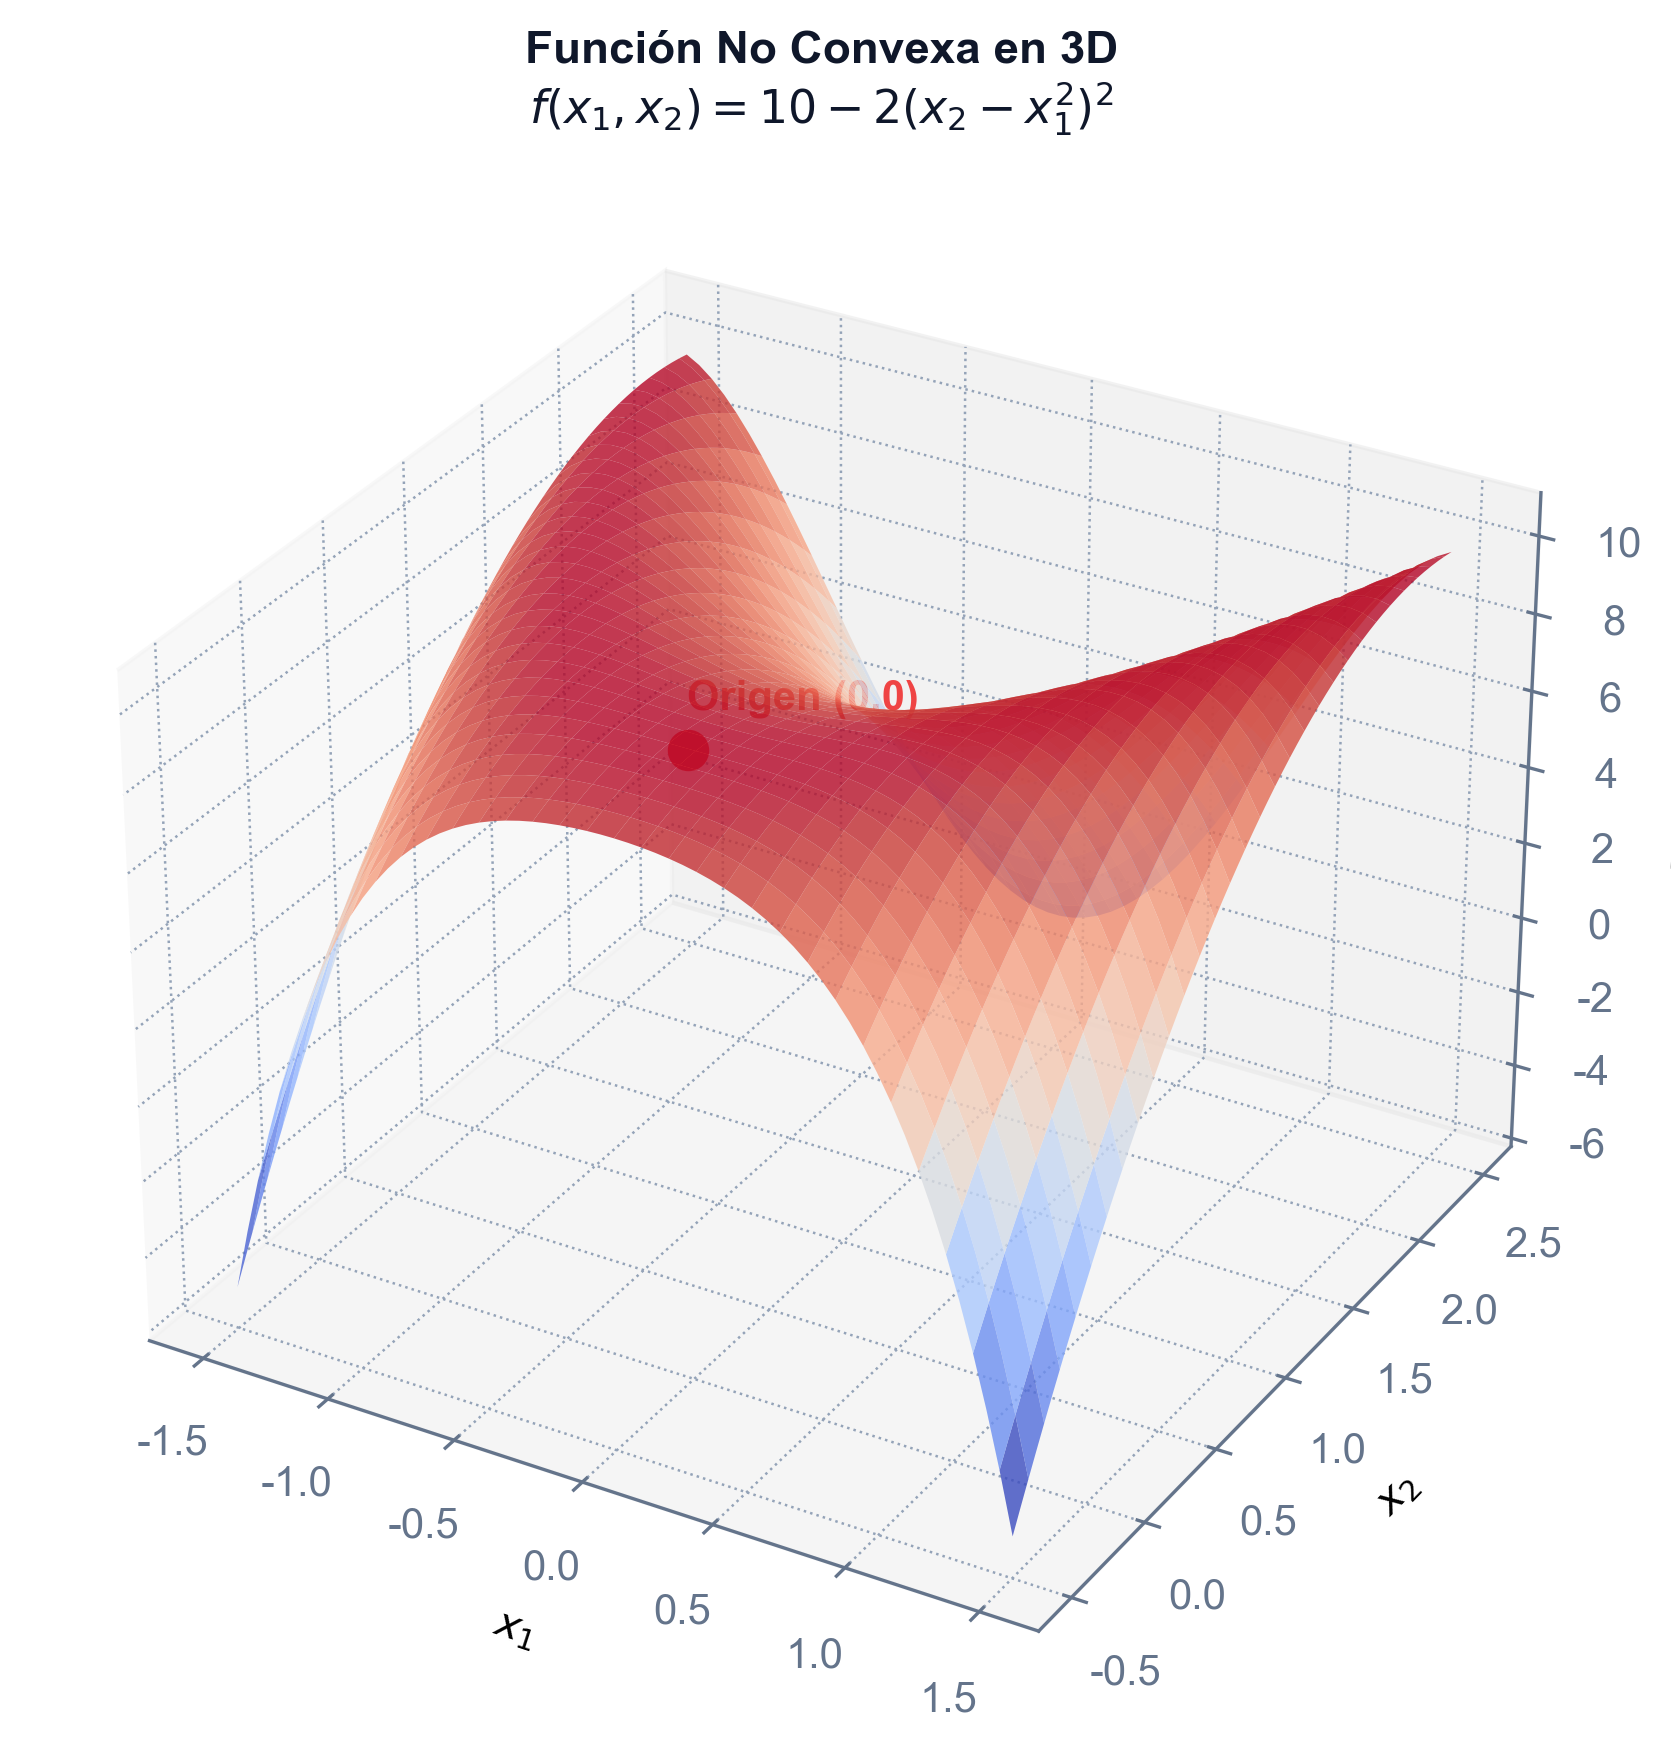
\includegraphics[width=0.7\linewidth,height=\textheight,keepaspectratio]{images/funcion_no_convexa_3d.png}

  }

  \caption{\label{fig-funcion-no-convexa-3d}Gráfica tridimensional de la
  función no convexa \(f(x_1, x_2) = 10 - 2(x_2 - x_1^2)^2\), destacando
  el origen de coordenadas donde es localmente cóncava}

  \end{figure}%
\item
  \textbf{Ejemplo 3}:
  \[ f(x, y, z) = x^2 + 3y^2 + z^2 + xy - 4z - 5x + 14 \] Su hessiana es
  constante:
  \[ \nabla^2 f = \begin{pmatrix} 2 & 1 & 0 \\ 1 & 6 & 0 \\ 0 & 0 & 2 \end{pmatrix} \]
  Menores principales: \(M_1 = 2 > 0\), \(M_2 = 11 > 0\),
  \(M_3 = 22 > 0\). Al ser definida positiva, la función es
  estrictamente convexa en todo el espacio.
\end{itemize}

\end{tcolorbox}

\section{Óptimos de una función
convexa}\label{uxf3ptimos-de-una-funciuxf3n-convexa}

La convexidad de una función no es simplemente una propiedad geométrica
elegante, sino el pilar fundamental que transforma la resolución de
problemas de optimización de una tarea localmente incierta a una
globalmente garantizada. En el análisis no convexo general, los
algoritmos numéricos pueden quedar atrapados en mínimos locales que no
ofrecen información sobre el mejor valor absoluto de la función. En
cambio, bajo hipótesis de convexidad, la estructura del espacio asegura
que cualquier mínimo local se extienda de forma global, facilitando
enormemente la búsqueda de soluciones óptimas.

\begin{tcolorbox}[enhanced jigsaw, toprule=.15mm, opacitybacktitle=0.6, coltitle=black, colbacktitle=quarto-callout-important-color!10!white, title=\textcolor{quarto-callout-important-color}{\faExclamation}\hspace{0.5em}{Teorema fundamental de la optimización convexa}, arc=.35mm, rightrule=.15mm, toptitle=1mm, breakable, bottomtitle=1mm, titlerule=0mm, colback=white, opacityback=0, leftrule=.75mm, colframe=quarto-callout-important-color-frame, left=2mm, bottomrule=.15mm]

Sea \(f: \mathcal{S} \to \mathbb{R}\) una función convexa sobre un
conjunto convexo \(\mathcal{S}\).

\begin{enumerate}
\def\labelenumi{\arabic{enumi}.}
\tightlist
\item
  \textbf{Cualquier mínimo local de \(f\) en \(\mathcal{S}\) es también
  un mínimo global}.
\item
  \textbf{Si la función \(f\) es estrictamente convexa, el mínimo global
  (si existe) es único}.
\end{enumerate}

\emph{Demostración}:

\begin{enumerate}
\def\labelenumi{\arabic{enumi}.}
\tightlist
\item
  Sea \(x^*\) un mínimo local de \(f\) en \(\mathcal{S}\). Por
  definición, existe un radio \(\epsilon > 0\) tal que
  \(f(x) \ge f(x^*)\) para todo \(x \in \mathcal{S}\) con
  \(\|x - x^*\| < \epsilon\). Supongamos por contradicción que \(x^*\)
  no es un mínimo global, lo que implica que existe un punto
  \(y \in \mathcal{S}\) tal que \(f(y) < f(x^*)\). Construimos una
  combinación lineal convexa de ambos puntos:
  \(x(\lambda) = \lambda y + (1-\lambda) x^*\) para
  \(\lambda \in (0, 1)\). Como el dominio \(\mathcal{S}\) es convexo,
  \(x(\lambda) \in \mathcal{S}\). Elegimos un \(\lambda\)
  suficientemente pequeño de forma que el punto \(x(\lambda)\) entre
  dentro de la bola de radio \(\epsilon\) alrededor de \(x^*\).
  Aplicando la propiedad de convexidad de \(f\):
  \[ f(x(\lambda)) \le \lambda f(y) + (1 - \lambda) f(x^*) < \lambda f(x^*) + (1 - \lambda) f(x^*) = f(x^*) \]
  Obtenemos que \(f(x(\lambda)) < f(x^*)\), lo cual contradice
  directamente la suposición de que \(x^*\) es un mínimo local. Por
  tanto, no puede existir tal punto \(y\), y \(x^*\) es un mínimo
  global.
\item
  Supongamos que \(f\) es estrictamente convexa y que existen dos
  mínimos globales distintos, \(x^*\) e \(y^*\), con
  \(f(x^*) = f(y^*) = \alpha\). Sea el punto medio
  \(z = \frac{1}{2} x^* + \frac{1}{2} y^* \in \mathcal{S}\). Por la
  convexidad estricta de \(f\):
  \[ f(z) < \frac{1}{2} f(x^*) + \frac{1}{2} f(y^*) = \alpha \] Resulta
  que \(f(z) < \alpha\), lo que contradice que \(\alpha\) sea el valor
  mínimo de la función. Por tanto, el mínimo global debe ser único.
  \(\blacksquare\)
\end{enumerate}

\end{tcolorbox}

Una vez establecida la equivalencia entre mínimos locales y globales, el
siguiente paso consiste en deducir criterios analíticos que nos permitan
identificar de forma unívoca si un determinado punto factible \(x^*\)
es, en efecto, un mínimo global del problema. Esto se logra traduciendo
el comportamiento geométrico de la función en herramientas diferenciales
(gradientes) o subdifenciales (para funciones no suaves), lo que da
origen a las condiciones variacionales de optimalidad:

\begin{itemize}
\tightlist
\item
  \textbf{Caracterización con subgradientes}: Un punto \(x^*\) es mínimo
  global de la función convexa \(f\) en \(\mathcal{S}\) si y solo si el
  vector nulo \(0\) es un subgradiente de \(f\) en \(x^*\):
  \[ 0 \in \partial f(x^*) \]
\item
  \textbf{Caracterización variacional diferenciable}: Si la función
  \(f\) es diferenciable en todo su dominio, entonces un punto \(x^*\)
  es un mínimo global en \(\mathcal{S}\) si y solo si:
  \[ \nabla f(x^*)^T (x - x^*) \ge 0, \quad \forall x \in \mathcal{S} \]
  \emph{Interpretación geométrica}: Esta condición establece que el
  gradiente \(\nabla f(x^*)\) forma un ángulo agudo u obtuso (de
  \(90^\circ\) o superior) con cualquier dirección admisible \(x - x^*\)
  que apunte desde el óptimo hacia el interior del conjunto factible
  \(\mathcal{S}\). Geométricamente, esto significa que no existen
  direcciones de descenso factibles en dicho punto.
\end{itemize}

\begin{tcolorbox}[enhanced jigsaw, toprule=.15mm, opacitybacktitle=0.6, coltitle=black, colbacktitle=quarto-callout-important-color!10!white, title=\textcolor{quarto-callout-important-color}{\faExclamation}\hspace{0.5em}{Teorema: Caracterización del conjunto de soluciones óptimas}, arc=.35mm, rightrule=.15mm, toptitle=1mm, breakable, bottomtitle=1mm, titlerule=0mm, colback=white, opacityback=0, leftrule=.75mm, colframe=quarto-callout-important-color-frame, left=2mm, bottomrule=.15mm]

Sea \(f: \mathcal{S} \to \mathbb{R}\) una función convexa y
diferenciable sobre el conjunto convexo \(\mathcal{S}\). Si existe al
menos un mínimo global \(x_0 \in \mathcal{S}\), entonces el conjunto de
todas las soluciones óptimas \(\mathcal{S}^*\) viene caracterizado por:
\[ \mathcal{S}^* = \{ x \in \mathcal{S} \mid \nabla f(x_0)^T(x - x_0) \ge 0 \quad \text{y} \quad \nabla f(x) = \nabla f(x_0) \} \]

\emph{Demostración}: Denotemos por \(\hat{\mathcal{S}}\) al conjunto de
soluciones óptimas globales. Queremos probar que
\(\mathcal{S}^* = \hat{\mathcal{S}}\).

\begin{itemize}
\item
  \textbf{Inclusión \(\mathcal{S}^* \subseteq \hat{\mathcal{S}}\)}: Sea
  \(x_1 \in \mathcal{S}^*\). Por definición de \(\mathcal{S}^*\), se
  tiene que \(x_1 \in \mathcal{S}\) y \(\nabla f(x_1) = \nabla f(x_0)\).
  Por ser \(f\) convexa y diferenciable, aplicando la caracterización de
  primer orden en el punto \(x_1\):
  \[ f(x_0) \ge f(x_1) + \nabla f(x_1)^T (x_0 - x_1) \] Sustituyendo
  \(\nabla f(x_1) = \nabla f(x_0)\) y reordenando:
  \[ f(x_0) \ge f(x_1) + \nabla f(x_0)^T (x_0 - x_1) = f(x_1) - \nabla f(x_0)^T (x_1 - x_0) \]
  Como por definición de \(\mathcal{S}^*\) se cumple que
  \(\nabla f(x_0)^T(x_1 - x_0) \ge 0\), entonces:
  \[ f(x_0) \ge f(x_1) \] Por otro lado, como \(x_0\) es un mínimo
  global, se tiene de forma necesaria que \(f(x_1) \ge f(x_0)\). Por
  consiguiente, \(f(x_1) = f(x_0)\), lo que demuestra que \(x_1\) es
  también un mínimo global, es decir, \(x_1 \in \hat{\mathcal{S}}\).
\item
  \textbf{Inclusión \(\hat{\mathcal{S}} \subseteq \mathcal{S}^*\)}: Sea
  \(x_1 \in \hat{\mathcal{S}}\) (un mínimo global), de modo que
  \(f(x_1) = f(x_0)\). Por la caracterización de primer orden en
  \(x_0\):
  \[ f(x_1) \ge f(x_0) + \nabla f(x_0)^T (x_1 - x_0) \implies 0 \ge \nabla f(x_0)^T (x_1 - x_0) \]
  Sin embargo, como \(x_0\) es un mínimo global, la condición
  variacional en \(x_0\) exige que \(\nabla f(x_0)^T (x_1 - x_0) \ge 0\)
  para todo \(x_1 \in \mathcal{S}\). De ambas desigualdades resulta:
  \[ \nabla f(x_0)^T (x_1 - x_0) = 0 \] De forma simétrica,
  intercambiando el papel de \(x_1\) y \(x_0\) (ya que ambos son óptimos
  y \(f(x_1) = f(x_0)\)), se deduce que:
  \[ \nabla f(x_1)^T (x_0 - x_1) = 0 \] Sumando ambas igualdades:
  \[ (\nabla f(x_0) - \nabla f(x_1))^T (x_0 - x_1) = 0 \] Por el teorema
  fundamental del cálculo multivariable, podemos expresar la diferencia
  de gradientes a través de la integral de la matriz hessiana a lo largo
  del segmento que une ambos puntos:
  \[ \nabla f(x_0) - \nabla f(x_1) = G (x_0 - x_1) \] donde
  \(G = \int_{0}^1 \nabla^2 f(x_1 + \lambda (x_0 - x_1)) d\lambda\) es
  una matriz semidefinida positiva (puesto que por convexidad la
  hessiana en todo punto de la trayectoria es semidefinida positiva).
  Sustituyendo:
  \[ 0 = (x_0 - x_1)^T (\nabla f(x_0) - \nabla f(x_1)) = (x_0 - x_1)^T G (x_0 - x_1) \]
  Como \(G \succeq 0\) es semidefinida positiva, para que esta forma
  cuadrática sea nula se requiere analíticamente que
  \(G(x_0 - x_1) = \mathbf{0}\). Esto implica que:
  \[ \nabla f(x_0) - \nabla f(x_1) = \mathbf{0} \implies \nabla f(x_1) = \nabla f(x_0) \]
  Por tanto, \(x_1\) verifica ambas condiciones y pertenece a
  \(\mathcal{S}^*\). \(\blacksquare\)
\end{itemize}

\end{tcolorbox}

\begin{tcolorbox}[enhanced jigsaw, toprule=.15mm, opacitybacktitle=0.6, coltitle=black, colbacktitle=quarto-callout-note-color!10!white, title=\textcolor{quarto-callout-note-color}{\faInfo}\hspace{0.5em}{Corolario: Caracterización del conjunto de óptimos mediante igualdad}, arc=.35mm, rightrule=.15mm, toptitle=1mm, breakable, bottomtitle=1mm, titlerule=0mm, colback=white, opacityback=0, leftrule=.75mm, colframe=quarto-callout-note-color-frame, left=2mm, bottomrule=.15mm]

Bajo las mismas hipótesis del teorema anterior, el conjunto de
soluciones óptimas \(\mathcal{S}^*\) también puede expresarse
alternativamente mediante la condición de igualdad del gradiente:
\[ \mathcal{S}^* = \{ x \in \mathcal{S} \mid \nabla f(x_0)^T (x - x_0) = 0 \} \]

\emph{Demostración}: Es inmediata a partir de que en la demostración
anterior se probó que para cualquier óptimo
\(x_1 \in \hat{\mathcal{S}}\) se verifica necesariamente que
\(\nabla f(x_0)^T (x_1 - x_0) = 0\), mientras que para cualquier punto
que satisfaga esta igualdad, la caracterización de primer orden
garantiza que \(f(x_1) \le f(x_0)\), forzando la optimalidad.
\(\blacksquare\)

\end{tcolorbox}

\begin{tcolorbox}[enhanced jigsaw, toprule=.15mm, opacitybacktitle=0.6, coltitle=black, colbacktitle=quarto-callout-note-color!10!white, title=\textcolor{quarto-callout-note-color}{\faInfo}\hspace{0.5em}{Corolario: Caso de funciones cuadráticas y dominios poliédricos}, arc=.35mm, rightrule=.15mm, toptitle=1mm, breakable, bottomtitle=1mm, titlerule=0mm, colback=white, opacityback=0, leftrule=.75mm, colframe=quarto-callout-note-color-frame, left=2mm, bottomrule=.15mm]

Si la función objetivo \(f\) es cuadrática de la forma
\(f(x) = c^T x + \frac{1}{2} x^T H x\) y el dominio factible
\(\mathcal{S}\) es un poliedro, entonces el conjunto de soluciones
óptimas \(\mathcal{S}^*\) es a su vez un poliedro expresable por el
sistema de ecuaciones lineales:
\[ \mathcal{S}^* = \{ x \in \mathcal{S} \mid c^T(x - x_0) = 0 \text{ y } H(x - x_0) = \mathbf{0} \} \]

\emph{Demostración}: Considerando que el gradiente de una función
cuadrática es \(\nabla f(x) = c + H x\), la condición del teorema
anterior exige
\(\nabla f(x) = \nabla f(x_0) \implies c + H x = c + H x_0 \implies H(x - x_0) = \mathbf{0}\).
Además, la condición de igualdad del gradiente resulta en:
\[ \nabla f(x_0)^T (x - x_0) = (c + H x_0)^T (x - x_0) = c^T (x - x_0) + (x-x_0)^T H x_0 = 0 \]
Puesto que \(H(x-x_0) = \mathbf{0} \implies H x = H x_0\), la simetría
de \(H\) nos da \((x-x_0)^T H x_0 = x_0^T H(x-x_0) = 0\), reduciendo la
ecuación a \(c^T(x-x_0) = 0\). \(\blacksquare\)

\end{tcolorbox}

Mientras que la minimización de funciones convexas es un problema
sumamente bien estructurado donde cualquier mínimo local es global, el
problema de maximización de funciones convexas (o, equivalentemente,
minimización de funciones cóncavas) presenta una naturaleza
completamente distinta. En este caso, el óptimo no tiende a situarse en
el interior del dominio, sino en sus extremos o fronteras. Para
caracterizar analíticamente estos máximos locales, formulamos la
condición necesaria de optimalidad de primer orden en términos de
subgradientes:

Mientras que la minimización de funciones convexas es un problema
sumamente bien estructurado donde cualquier mínimo local es global, el
problema de maximización de funciones convexas (o, equivalentemente,
minimización de funciones cóncavas) presenta una naturaleza
completamente distinta. En este caso, el óptimo no tiende a situarse en
el interior del dominio, sino en sus extremos o fronteras. Para
caracterizar analíticamente estos máximos locales, formulamos la
condición necesaria de optimalidad de primer orden en términos de
subgradientes:

\begin{tcolorbox}[enhanced jigsaw, toprule=.15mm, opacitybacktitle=0.6, coltitle=black, colbacktitle=quarto-callout-important-color!10!white, title=\textcolor{quarto-callout-important-color}{\faExclamation}\hspace{0.5em}{Teorema: Condición necesaria para máximos locales de funciones convexas}, arc=.35mm, rightrule=.15mm, toptitle=1mm, breakable, bottomtitle=1mm, titlerule=0mm, colback=white, opacityback=0, leftrule=.75mm, colframe=quarto-callout-important-color-frame, left=2mm, bottomrule=.15mm]

Sea el problema de maximizar \(f(x)\) sujeto a \(x \in \mathcal{S}\),
donde \(f: \mathcal{S} \to \mathbb{R}\) es una función convexa y
\(\mathcal{S}\) es un conjunto convexo no vacío de \(\mathbb{R}^n\). Si
\(x_0 \in \mathcal{S}\) es un óptimo local para este problema de
maximización, entonces:
\[ \xi^T(x - x_0) \le 0, \quad \forall x \in \mathcal{S} \] donde
\(\xi\) es cualquier subgradiente de \(f\) en \(x_0\)
(\(\xi \in \partial f(x_0)\)).

\emph{Demostración}: Sea \(x_0\) un óptimo local para el problema de
maximización de la función convexa \(f\). Por definición, existe un
entorno \(N_\epsilon(x_0)\) tal que \(f(x) \le f(x_0)\) para todo
\(x \in \mathcal{S} \cap N_\epsilon(x_0)\). Sea \(x\) cualquier punto de
\(\mathcal{S}\). Por la convexidad de \(\mathcal{S}\), para cualquier
parámetro \(\lambda > 0\) suficientemente pequeño, el punto intermedio
\(x_\lambda = x_0 + \lambda(x - x_0) \in \mathcal{S}\) y pertenece al
entorno \(N_\epsilon(x_0)\). Por consiguiente:
\[ f(x_0 + \lambda(x - x_0)) \le f(x_0) \] Por otra parte, sea
\(\xi \in \partial f(x_0)\) un subgradiente de \(f\) en \(x_0\). Por
definición de subgradiente:
\[ f(x_0 + \lambda(x - x_0)) \ge f(x_0) + \xi^T [x_0 + \lambda(x - x_0) - x_0] = f(x_0) + \lambda \xi^T(x - x_0) \]
Uniendo ambas inecuaciones:
\[ f(x_0) \ge f(x_0) + \lambda \xi^T(x - x_0) \implies \lambda \xi^T(x - x_0) \le 0 \]
Como \(\lambda > 0\), dividiendo por \(\lambda\) se obtiene el
resultado: \[ \xi^T(x - x_0) \le 0 \] para cualquier subgradiente
\(\xi \in \partial f(x_0)\). \(\blacksquare\)

\end{tcolorbox}

\begin{tcolorbox}[enhanced jigsaw, toprule=.15mm, opacitybacktitle=0.6, coltitle=black, colbacktitle=quarto-callout-note-color!10!white, title=\textcolor{quarto-callout-note-color}{\faInfo}\hspace{0.5em}{Corolario: Caso diferenciable para máximos locales}, arc=.35mm, rightrule=.15mm, toptitle=1mm, breakable, bottomtitle=1mm, titlerule=0mm, colback=white, opacityback=0, leftrule=.75mm, colframe=quarto-callout-note-color-frame, left=2mm, bottomrule=.15mm]

Si la función convexa \(f\) es además diferenciable en todo el dominio
\(\mathcal{S}\), entonces la condición necesaria para que un punto
\(x_0 \in \mathcal{S}\) sea un óptimo local del problema de maximización
se simplifica a:
\[ \nabla f(x_0)^T (x - x_0) \le 0, \qquad \forall x \in \mathcal{S} \]

\end{tcolorbox}

Es fundamental remarcar que, a diferencia del caso de la minimización
(donde la condición variacional es necesaria y suficiente), la condición
de máximo local \(\nabla f(x_0)^T(x-x_0) \le 0\) para funciones convexas
es una condición necesaria extremadamente débil y \textbf{no es
suficiente} para garantizar un máximo local. De hecho, puntos que
corresponden a mínimos globales pueden cumplirla perfectamente, lo que
resalta la asimetría fundamental entre la búsqueda de mínimos y máximos
en el análisis convexo. Para ilustrar esta limitación teórica,
consideremos el siguiente contraejemplo clásico:

Como contraejemplo ilustrativo, consideremos la función convexa de una
variable \(f(x) = x^2\) definida en el dominio acotado
\(\mathcal{S} = [-1, 2]\). El máximo global de la función se alcanza en
la frontera derecha en \(x^* = 2\) (con un valor de 4). Sin embargo, en
el origen de coordenadas \(x_0 = 0\), el gradiente de la función es nulo
(\(\nabla f(0) = 0\)). Por consiguiente, se cumple trivialmente que:
\[ \nabla f(0)^T (x - 0) = 0 \le 0, \qquad \forall x \in [-1, 2] \] a
pesar de que en \(x_0 = 0\) la función alcanza su mínimo global absoluto
y no un máximo local, como se ilustra en la
Figura~\ref{fig-opt-contraejemplo-maximo}.

\begin{figure}

\centering{

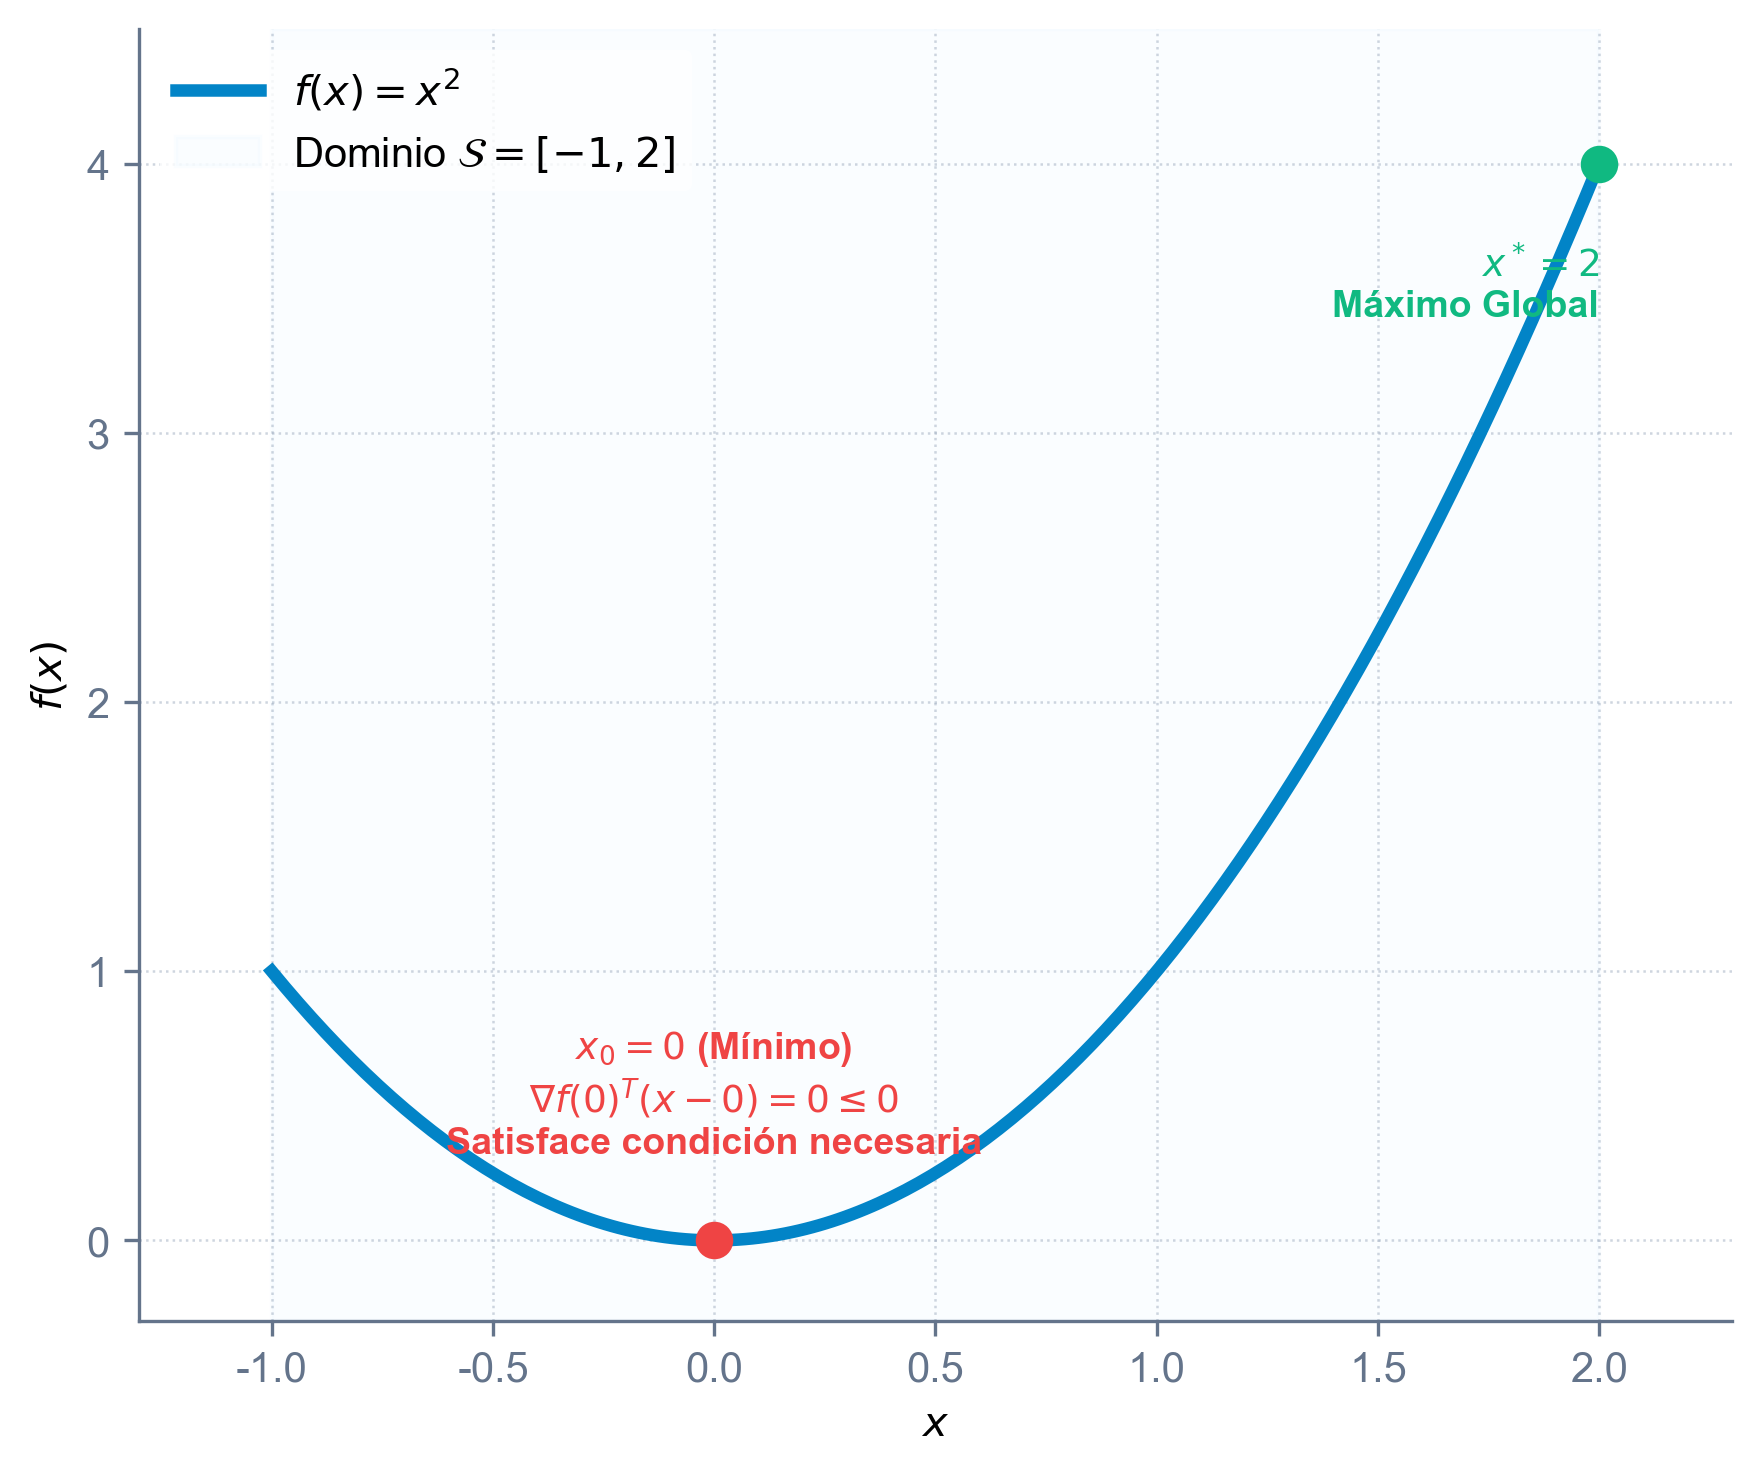
\includegraphics[width=0.6\linewidth,height=\textheight,keepaspectratio]{images/opt_contraejemplo_maximo.png}

}

\caption{\label{fig-opt-contraejemplo-maximo}Contraejemplo de la
condición necesaria para la maximización de funciones convexas en un
dominio acotado \([-1, 2]\), mostrando que en el mínimo \(x_0=0\) se
satisface la condición de gradiente nulo}

\end{figure}%

Para afianzar el uso de las condiciones de optimalidad basadas en
subgradientes y gradientes, tanto en problemas libres como restringidos
en la frontera del dominio, a continuación se analizan cuatro casos de
estudio prácticos detalladamente, mostrando cómo el subdiferencial y el
subgradiente se aplican tanto en problemas de una variable como en
problemas multivariables, y cómo determinan la optimalidad global (tanto
en puntos interiores como en la frontera del dominio).

\begin{tcolorbox}[enhanced jigsaw, toprule=.15mm, opacitybacktitle=0.6, coltitle=black, colbacktitle=quarto-callout-tip-color!10!white, title=\textcolor{quarto-callout-tip-color}{\faLightbulb}\hspace{0.5em}{Ejemplos: Análisis de optimalidad mediante gradientes y subgradientes}, arc=.35mm, rightrule=.15mm, toptitle=1mm, breakable, bottomtitle=1mm, titlerule=0mm, colback=white, opacityback=0, leftrule=.75mm, colframe=quarto-callout-tip-color-frame, left=2mm, bottomrule=.15mm]

\textbf{Ejemplo 1: Función no diferenciable definida por tramos en
\(\mathbb{R}\)}

Consideremos la función de una variable:
\[ f(x) = \begin{cases} x - 4 & \text{si } 1 \le x \le 4 \\ (x - 2)^2 - 4 & \text{en otro caso} \end{cases} \]
Esta función puede expresarse como el máximo de dos funciones convexas y
posee un punto de no diferenciabilidad (codo) en \(x^* = 1\), con un
subdiferencial dado por: \[ \partial f(1) = [-2, 1] \] Dado que el
vector nulo \(0\) pertenece al subdiferencial en este codo
(\(0 \in [-2, 1]\)), se satisface de forma necesaria y suficiente la
condición de optimalidad: \[ 0 \in \partial f(x^*) \] Por lo tanto,
\textbf{\(x^* = 1\) es el mínimo global} de la función, con un valor de
\(f(1) = -3\). En la gráfica, observamos que en dicho punto se puede
trazar una recta de soporte horizontal (pendiente cero) que queda
enteramente por debajo de la función.

\begin{figure}[H]

\centering{

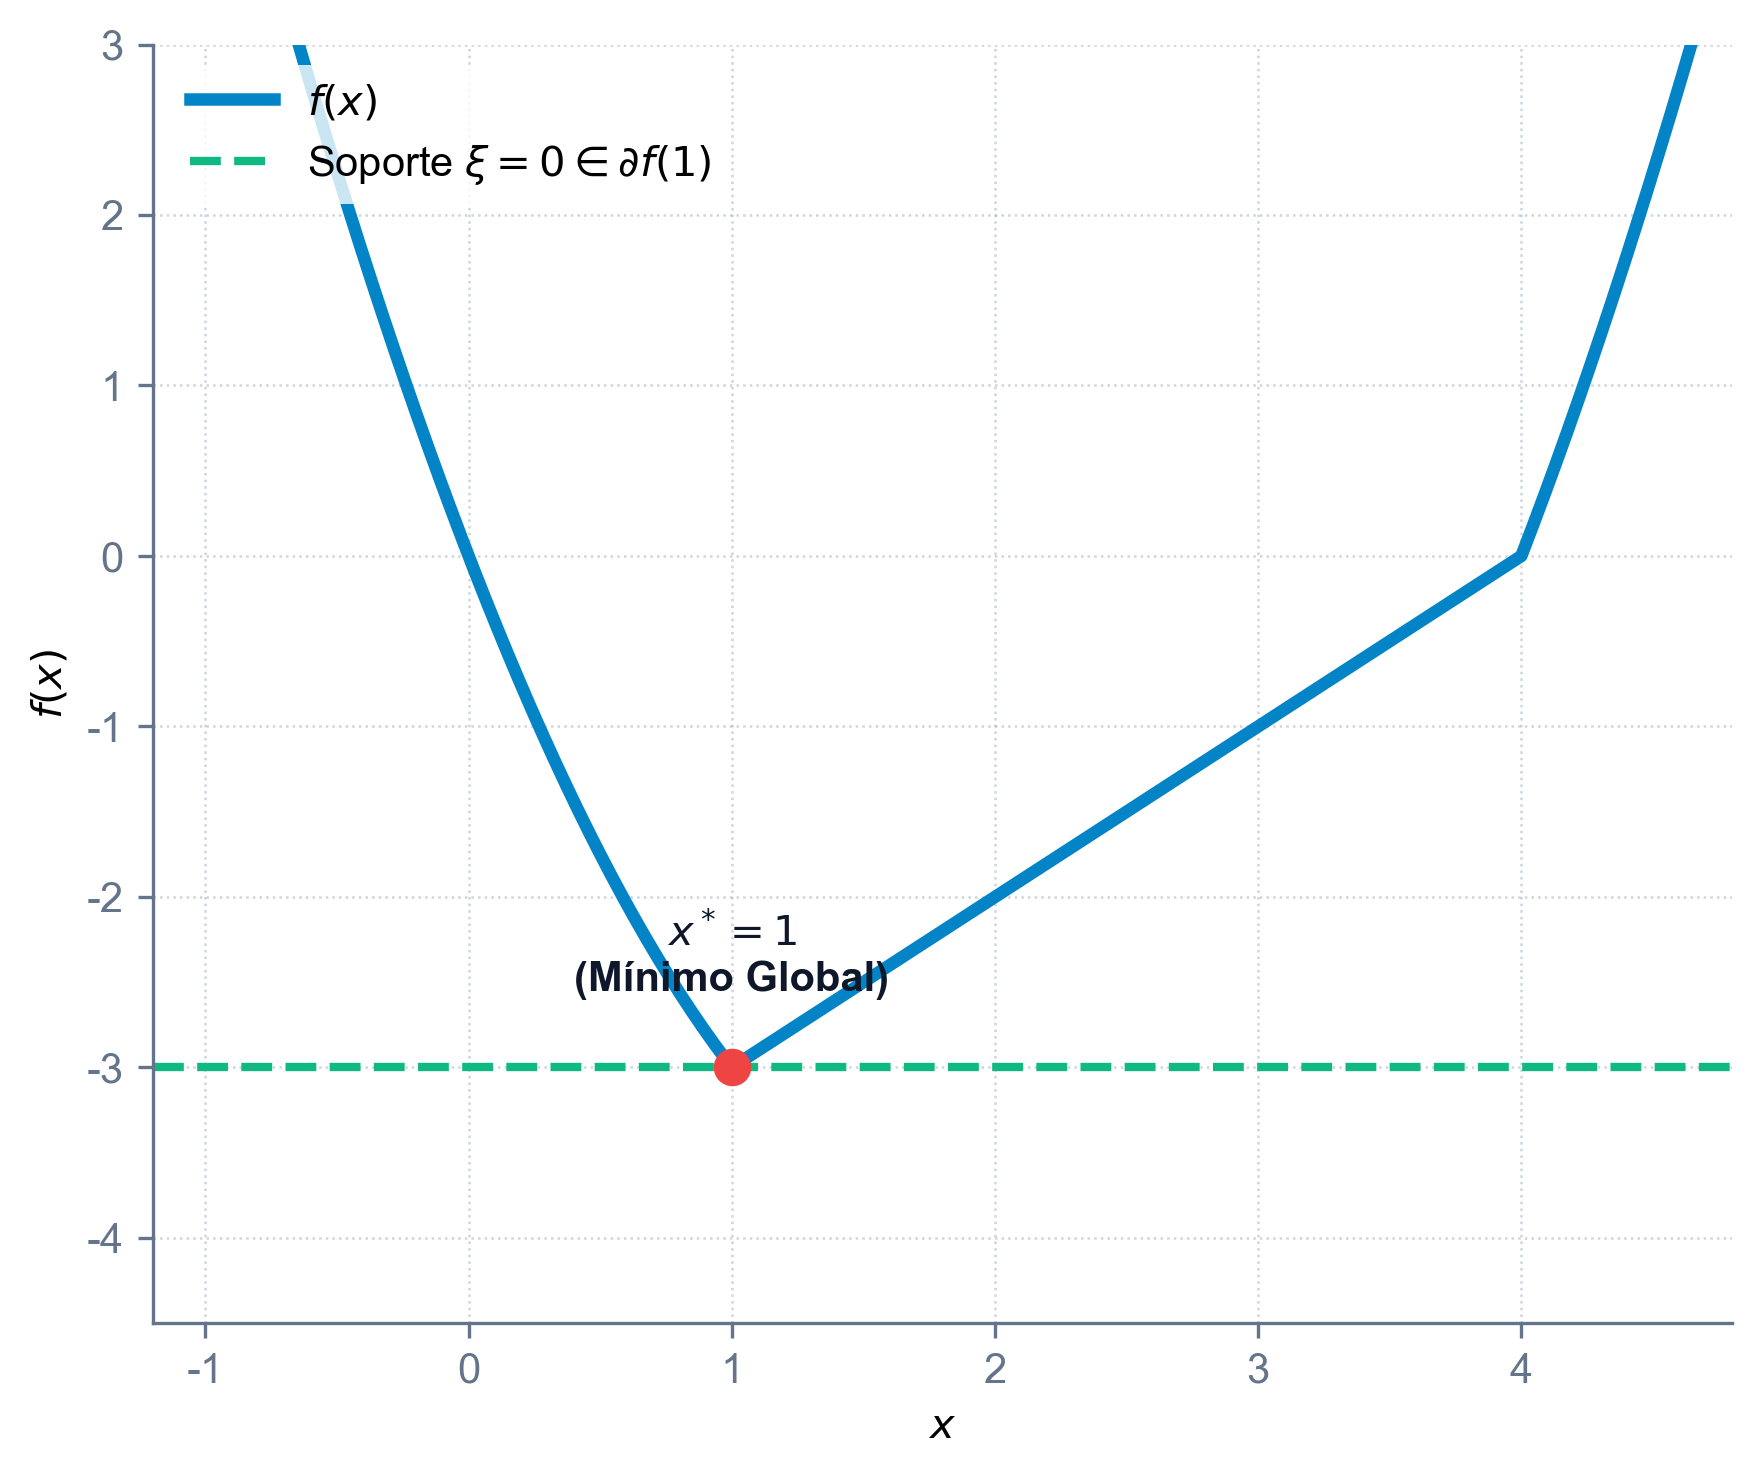
\includegraphics[width=0.6\linewidth,height=\textheight,keepaspectratio]{images/opt_ejemplo1_subgrad.png}

}

\caption{\label{fig-opt-ejemplo1-subgrad}Ejemplo 1: Mínimo global
situado en el punto singular o codo \(x^* = 1\) donde el subdiferencial
\([-2, 1]\) contiene al cero, lo que permite trazar una recta soporte de
pendiente nula}

\end{figure}%

\textbf{Ejemplo 2: Optimización en dominio restringido de
\(\mathbb{R}\)}

Consideremos la parábola convexa \(f(x) = (x-2)^2-4\) definida en el
dominio cerrado restringido \(\mathcal{S} = [3, 5]\). El mínimo
analítico global sin restricciones se sitúa en \(x = 2\), el cual es
exterior al conjunto factible \(\mathcal{S}\). El gradiente clásico de
la función en el punto frontera \(x^* = 3\) es \(\nabla f(3) = 2\). Para
que un punto de la frontera sea un mínimo sobre \(\mathcal{S}\),
cualquier dirección admisible hacia el interior del dominio
(\(x - x^* \ge 0\)) debe ser de no descenso. El subdiferencial
restringido a \(\mathcal{S}\) en el punto frontera \(x^* = 3\) es:
\[ \partial f_{\mathcal{S}}(3) = (-\infty, 2] \] Dado que el vector nulo
\(0\) pertenece a este subdiferencial restringido (\(0 \le 2\)),
concluimos que \textbf{\(x^* = 3\) es el mínimo global} de la función
sobre \(\mathcal{S}\). En la gráfica (ver la
Figura~\ref{fig-opt-ejemplo2-subgrad}) se muestra la parábola en la
región factible y cómo todas las pendientes \(\xi \le 2\) (incluyendo la
pendiente cero) actúan como planos soporte válidos para los puntos de
\(\mathcal{S}\).

\begin{figure}[H]

\centering{

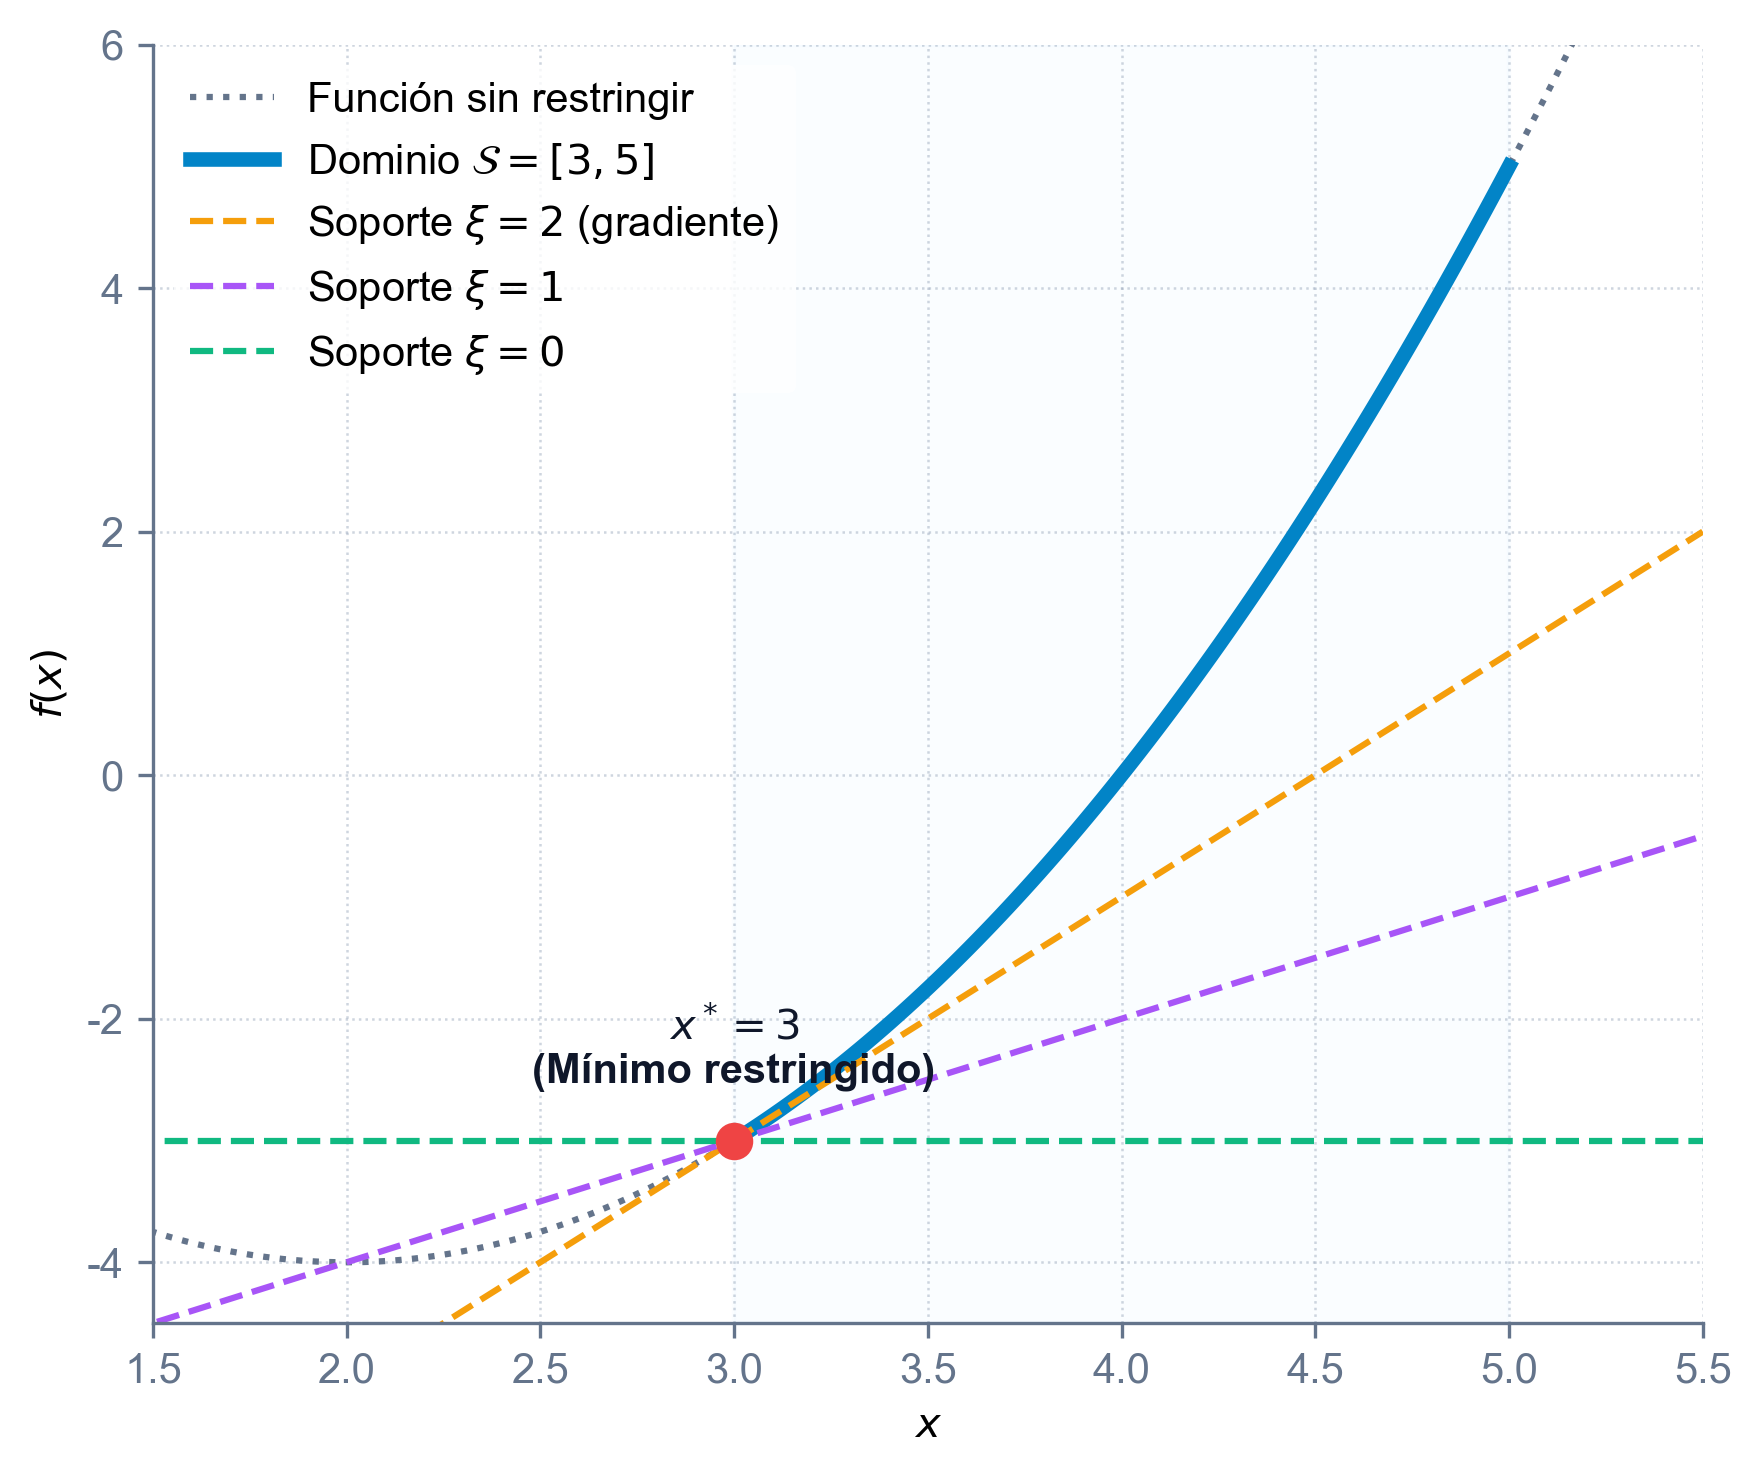
\includegraphics[width=0.6\linewidth,height=\textheight,keepaspectratio]{images/opt_ejemplo2_subgrad.png}

}

\caption{\label{fig-opt-ejemplo2-subgrad}Ejemplo 2: Mínimo global sobre
un dominio cerrado restringido \(\mathcal{S} = [3, 5]\) situado en la
frontera inferior \(x^* = 3\). Las rectas de pendiente \(\xi \le 2\)
soportan a la función para todo el dominio factible}

\end{figure}%

\textbf{Ejemplo 3: Minimización de distancia a un punto exterior en
\(\mathbb{R}^2\)}

Consideremos la función de distancia cuadrática al punto exterior
\((3, 2)\) dada por: \[ f(x_1, x_2) = (x_1 - 3)^2 + (x_2 - 2)^2 \] sobre
el conjunto convexo factible acotado \(\mathcal{S}\) definido por:
\[ \mathcal{S} = \{ (x_1, x_2) \in \mathbb{R}^2 \mid x_1^2 + x_2^2 \le 5, \ x_1 + 2x_2 \le 4, \ x_1 \ge 0, \ x_2 \ge 0 \} \]
El punto de \(\mathcal{S}\) geométricamente más cercano al punto
objetivo exterior \((3, 2)\) es el punto frontera \(x^* = (2, 1)\). El
gradiente en este óptimo es:
\[ \nabla f(2, 1) = \begin{pmatrix} -2 \\ -2 \end{pmatrix} \] La
condición variacional de optimalidad de primer orden exige que
\(\nabla f(x^*)^T (x - x^*) \ge 0\) para todo \(x \in \mathcal{S}\).
Evaluando el producto escalar:
\[ -2(x_1 - 2) - 2(x_2 - 1) \ge 0 \iff x_1 + x_2 \le 3 \] Esta
inecuación define un semiplano cuya frontera es la recta
\(x_1 + x_2 = 3\). Como se puede ver en la
Figura~\ref{fig-opt-ejemplo3-subgrad}, todo el conjunto factible
\(\mathcal{S}\) queda contenido en la región \(x_1 + x_2 \le 3\). Esto
significa que el gradiente apunta en dirección opuesta al interior de
\(\mathcal{S}\), y el hiperplano \(x_1 + x_2 = 3\) actúa como un plano
separador entre el conjunto factible y los contornos inferiores de la
función de distancia, confirmando que \textbf{\(x^* = (2, 1)\) es el
mínimo global} restringido.

\begin{figure}[H]

\centering{

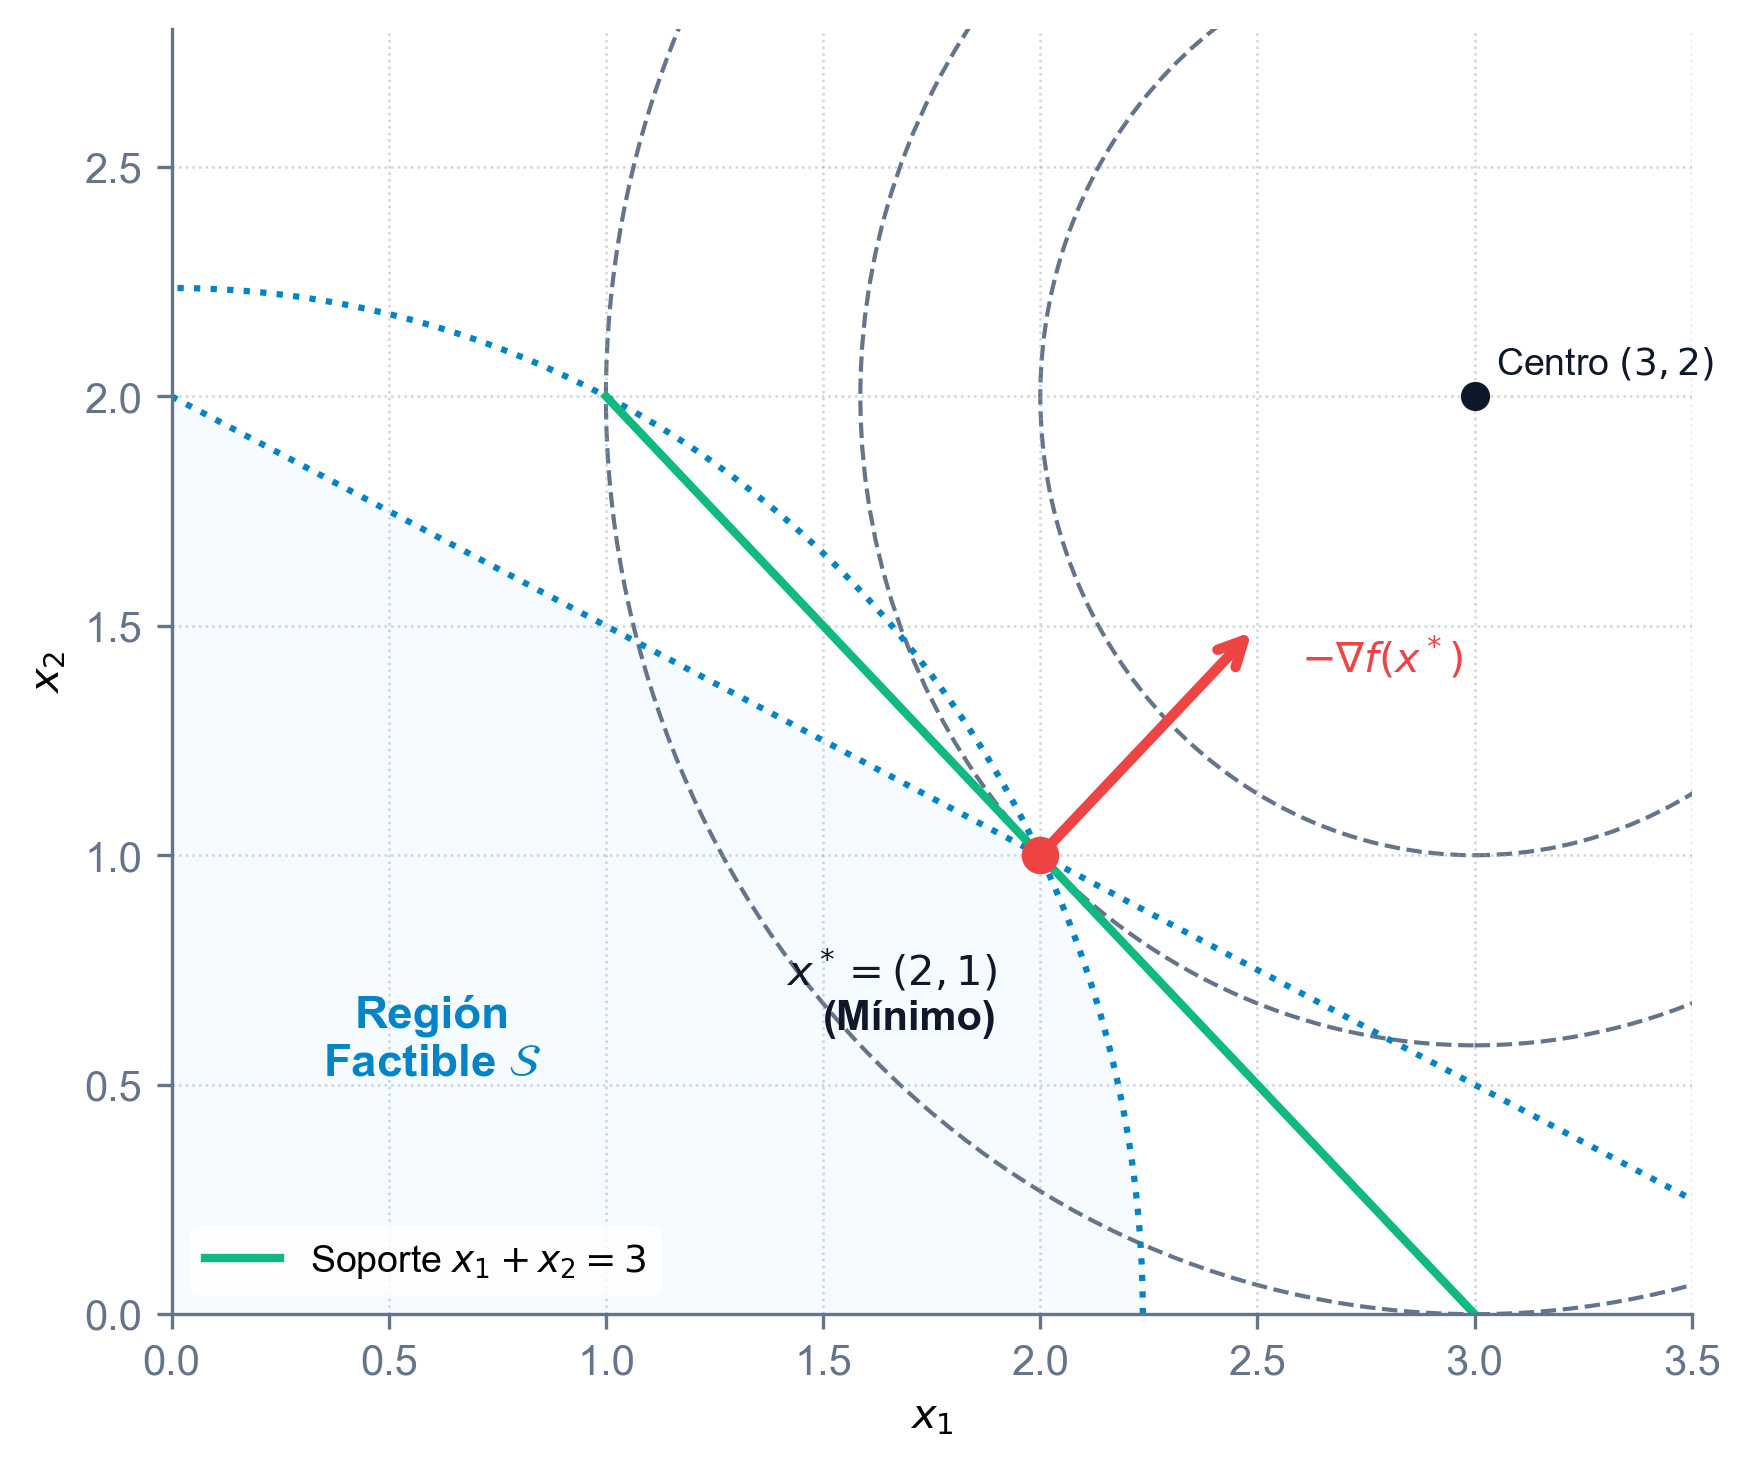
\includegraphics[width=0.6\linewidth,height=\textheight,keepaspectratio]{images/opt_ejemplo3_subgrad.png}

}

\caption{\label{fig-opt-ejemplo3-subgrad}Ejemplo 3: Minimización de
distancia cuadrática a un punto objetivo exterior \((3, 2)\) sobre un
dominio acotado en \(\mathbb{R}^2\). El óptimo se sitúa en la frontera
\(x^* = (2, 1)\) y el plano separador \(x_1+x_2=3\) es perpendicular al
gradiente}

\end{figure}%

\textbf{Ejemplo 4: Minimización de distancia a un punto interior en
\(\mathbb{R}^2\)}

Consideremos la misma función de distancia cuadrática y dominio del
Ejemplo 3, pero buscando el mínimo respecto al punto \((1, 1)\), que es
un punto interior del conjunto factible \(\mathcal{S}\) (puesto que
\(1^2+1^2=2 < 5\) y \(1+2(1)=3 < 4\)).
\[ f(x_1, x_2) = (x_1 - 1)^2 + (x_2 - 1)^2 \] Al ser el punto de
referencia interior al dominio factible, la solución óptima coincide
trivialmente con el propio punto de referencia: \(x^* = (1, 1)\). El
gradiente en dicho óptimo es:
\[ \nabla f(1, 1) = \begin{pmatrix} 0 \\ 0 \end{pmatrix} \] Como el
gradiente es nulo, el vector nulo \(0\) pertenece al subdiferencial
\(\partial f(1, 1) = \{\binom{0}{0}\}\), lo cual satisface la condición
de mínimo interior de forma inmediata. La
Figura~\ref{fig-opt-ejemplo4-subgrad} muestra los contornos circulares
de distancia concéntricos alrededor del óptimo dentro del poliedro.

\begin{figure}[H]

\centering{

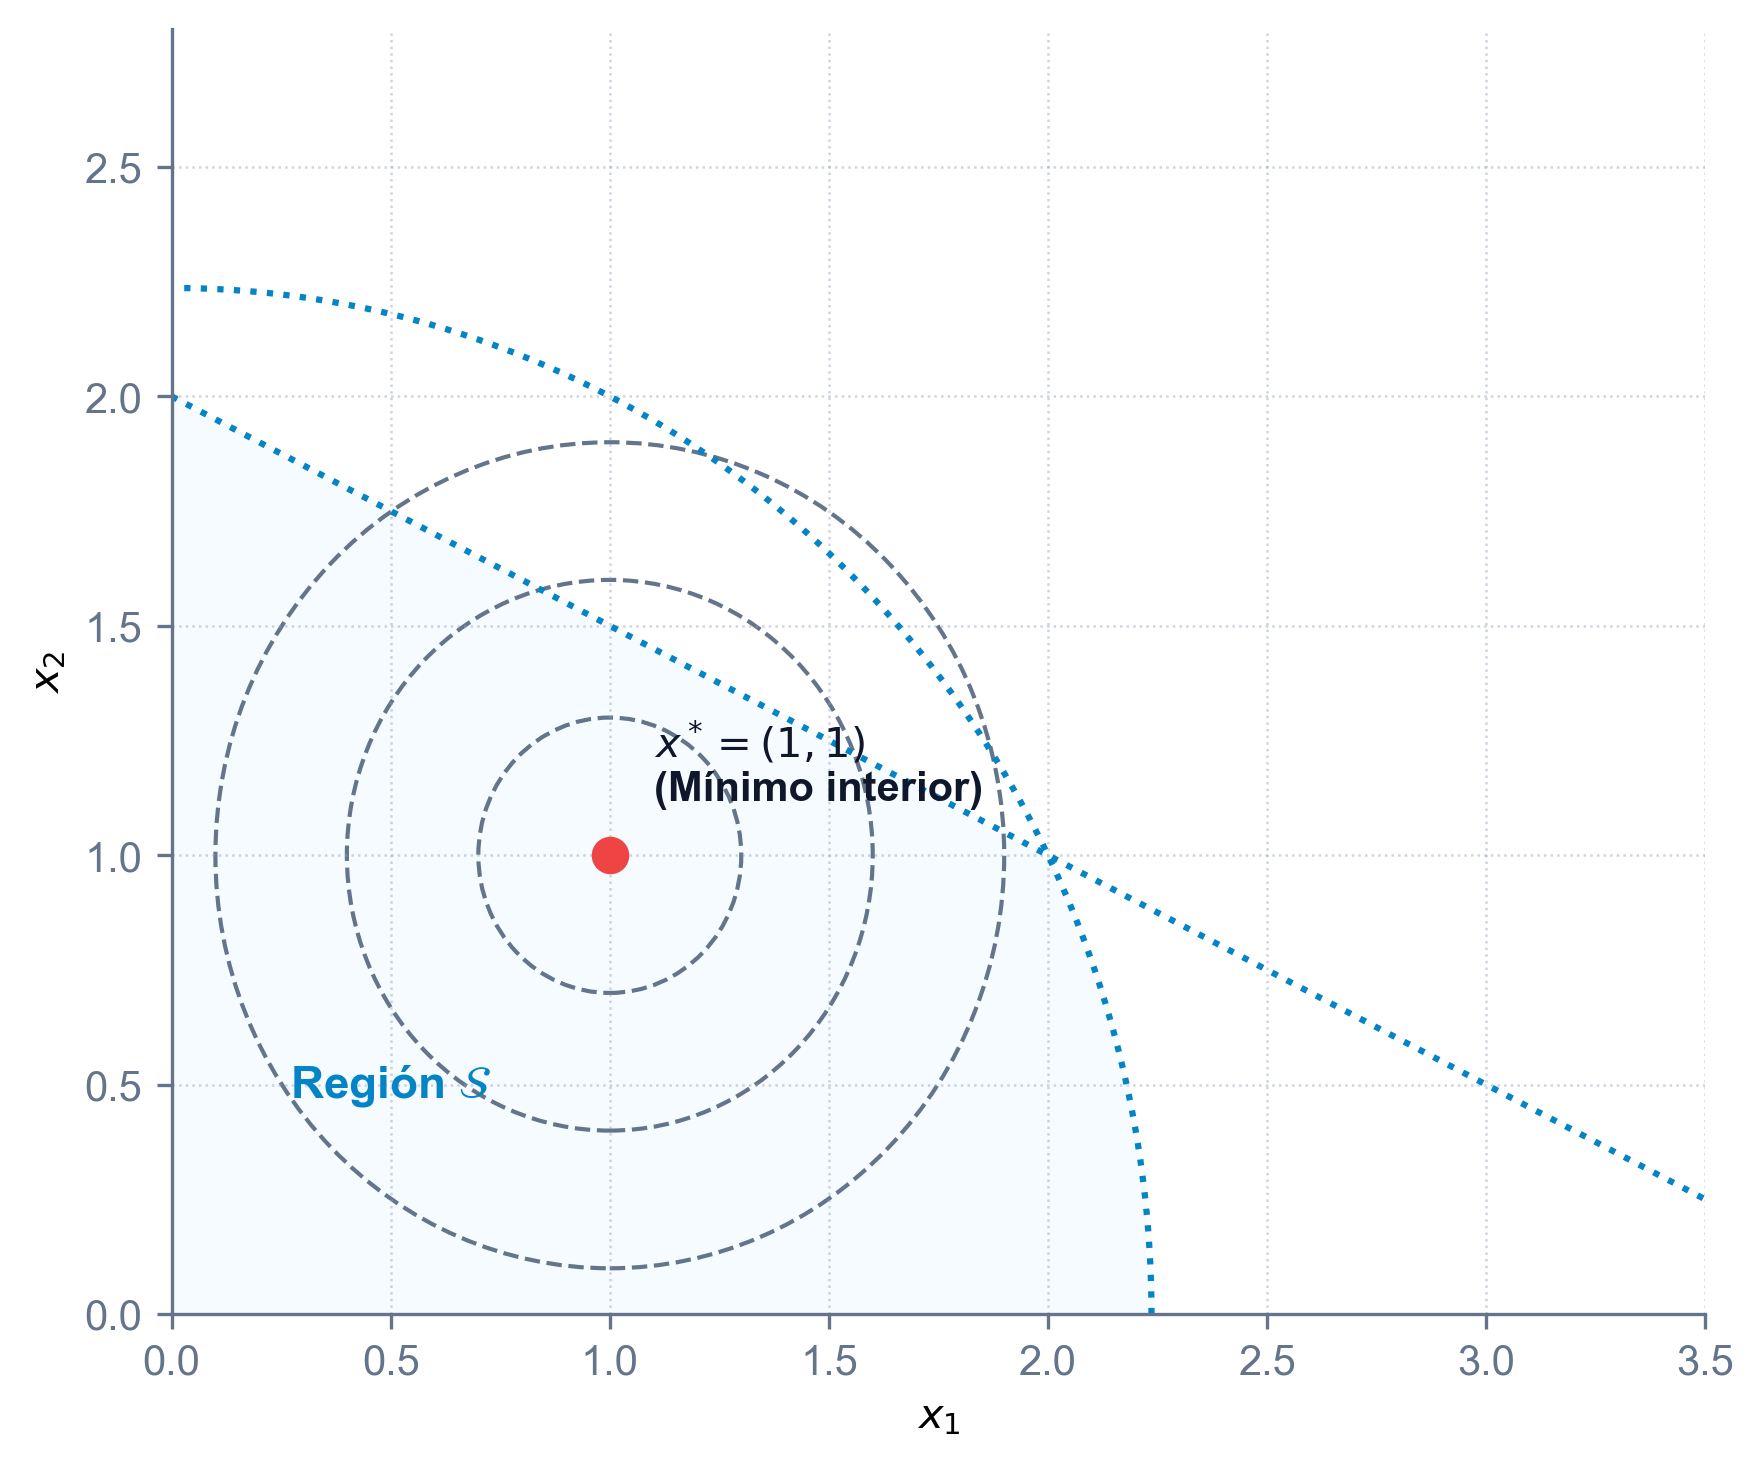
\includegraphics[width=0.6\linewidth,height=\textheight,keepaspectratio]{images/opt_ejemplo4_subgrad.png}

}

\caption{\label{fig-opt-ejemplo4-subgrad}Ejemplo 4: Minimización de
distancia cuadrática a un punto objetivo interior \((1, 1)\) en
\(\mathbb{R}^2\). Al estar el punto de referencia dentro del dominio
factible, el mínimo global se sitúa en \(x^* = (1, 1)\) con gradiente
nulo}

\end{figure}%

\end{tcolorbox}

\begin{tcolorbox}[enhanced jigsaw, toprule=.15mm, opacitybacktitle=0.6, coltitle=black, colbacktitle=quarto-callout-warning-color!10!white, title=\textcolor{quarto-callout-warning-color}{\faExclamationTriangle}\hspace{0.5em}{Advertencia: Maximización de funciones convexas}, arc=.35mm, rightrule=.15mm, toptitle=1mm, breakable, bottomtitle=1mm, titlerule=0mm, colback=white, opacityback=0, leftrule=.75mm, colframe=quarto-callout-warning-color-frame, left=2mm, bottomrule=.15mm]

La maximización de una función convexa es un problema no convexo y, por
tanto, sumamente complejo. Por un lado, las condiciones necesarias de
primer orden (como la existencia de un gradiente nulo en el interior)
suelen identificar mínimos locales en lugar de máximos. Por otro lado,
la maximización de una función convexa sobre un politopo compacto
\(\mathcal{S}\) garantiza que el máximo global se sitúa en alguno de los
puntos extremos (vértices) de dicho politopo (como se demostró en el
\hyperref[maximiza-poliedro]{Teorema de Maximización en Poliedros} en la
\hyperref[sec-puntos-extremos]{Sección 3.1}). Esto justifica que los
algoritmos de maximización convexa se centren exclusivamente en explorar
los vértices de la región factible.

\end{tcolorbox}

\section{Generalizaciones de la
convexidad}\label{generalizaciones-de-la-convexidad}

A pesar de la enorme utilidad de las funciones convexas en optimización,
la hipótesis de convexidad pura es en ocasiones demasiado restrictiva
para modelar múltiples problemas reales en economía, ingeniería y teoría
de juegos. En muchas aplicaciones prácticas, nos encontramos con
funciones que no tienen forma de ``cuenco'' o cuya hessiana no es
semidefinida positiva en todo su dominio, pero que conservan propiedades
fundamentales muy valiosas, como la convexidad de sus conjuntos de nivel
o la equivalencia entre mínimos locales y globales.

Con el objetivo de ampliar el alcance de las técnicas de optimización
global, el análisis convexo define generalizaciones que relajan las
exigencias algebraicas tradicionales. Entre estas generalizaciones
destacan las funciones cuasi-convexas, que preservan la naturaleza
convexa de sus conjuntos de nivel inferior, y las funciones
pseudo-convexas, que garantizan que el gradiente nulo actúe como un
criterio de mínimo global. A continuación se analiza la estructura,
teoremas y relaciones matemáticas de estas familias de funciones.

\subsection{Funciones cuasi-convexas}\label{funciones-cuasi-convexas}

La primera y más intuitiva de las generalizaciones de la convexidad
surge al relajar la condición algebraica sobre el perfil de la función y
concentrarnos en la geometría de sus conjuntos asociados. En lugar de
exigir que la gráfica completa de la función tenga una curvatura hacia
arriba, demandamos únicamente que sus cortes horizontales tengan forma
convexa. Es decir, una función se define como \textbf{cuasi-convexa} si
todos sus conjuntos de nivel inferior \(\mathcal{S}_\alpha\) son
convexos, lo que impide que la función vuelva a subir tras haber bajado,
evitando así mínimos locales separados por barreras (como se ilustra en
los casos unidimensionales de la
Figura~\ref{fig-funciones-cuasiconvexas-ejemplos}). Analíticamente, esta
exigencia geométrica se traduce en que el valor de la función en
cualquier punto intermedio de un segmento no puede superar al mayor de
los valores en los extremos:
\[ f(\lambda x_1 + (1 - \lambda) x_2) \le \max \{ f(x_1), f(x_2) \}, \quad \forall x_1, x_2 \in \mathcal{S}, \ \forall \lambda \in [0, 1] \]

\begin{figure}

\centering{

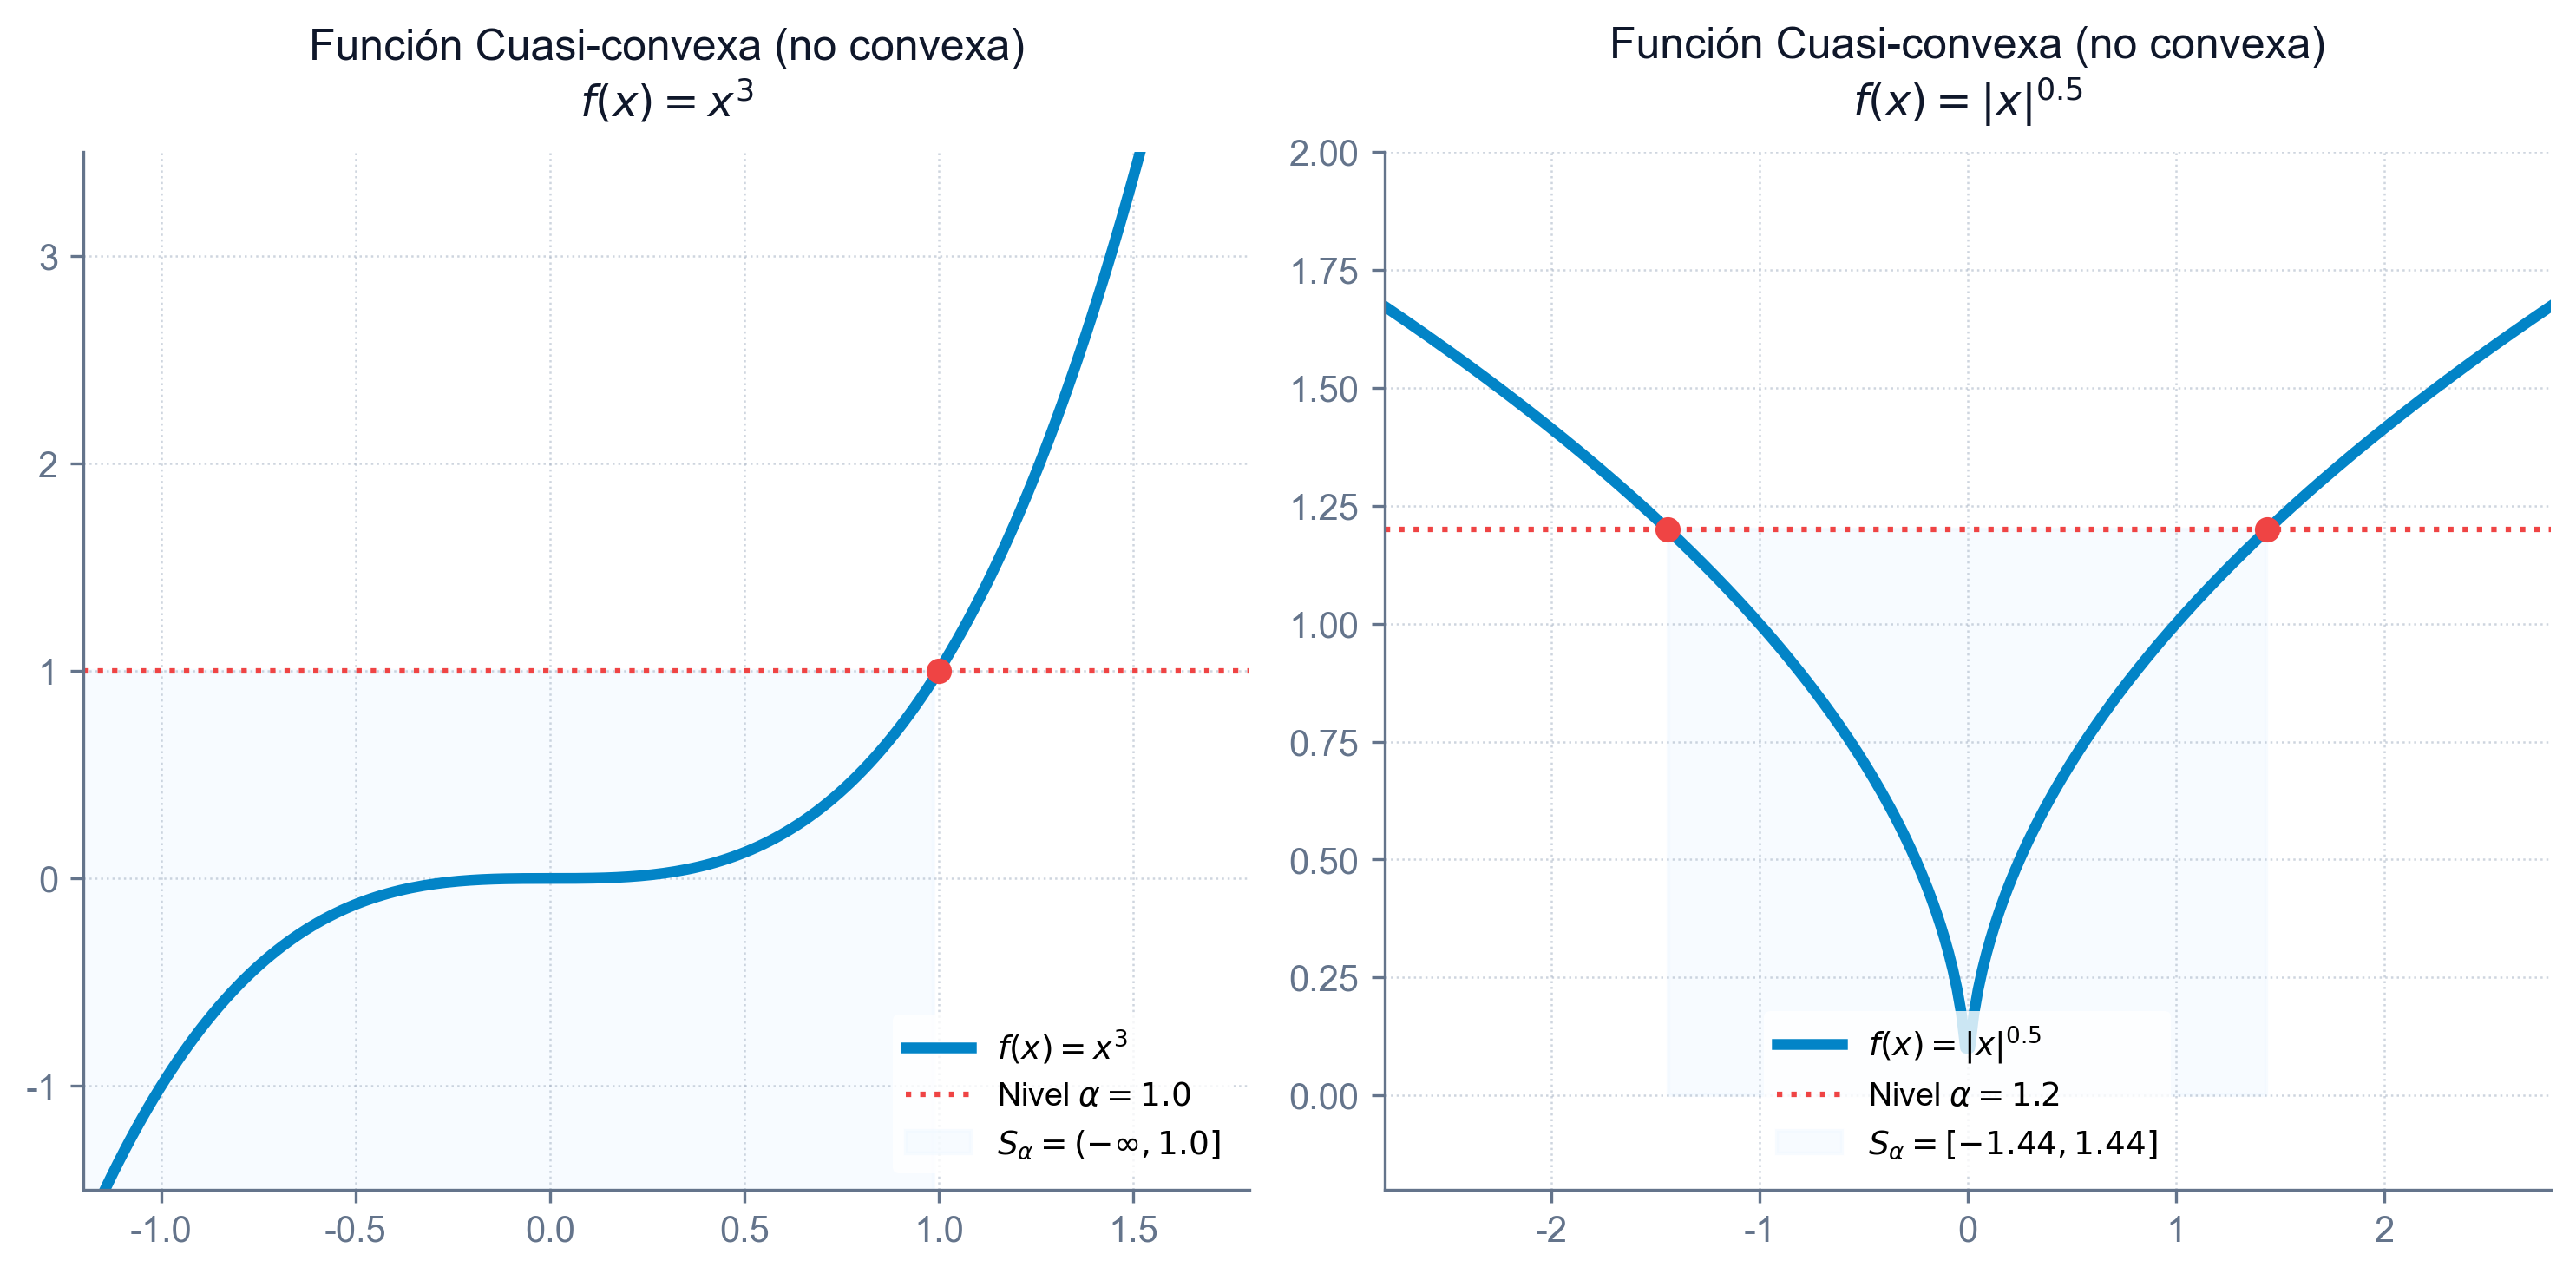
\includegraphics[width=0.85\linewidth,height=\textheight,keepaspectratio]{images/funciones_cuasiconvexas_ejemplos.png}

}

\caption{\label{fig-funciones-cuasiconvexas-ejemplos}Ejemplos de
funciones cuasi-convexas no convexas en una dimensión: \(f(x)=x^3\)
(izquierda) y \(f(x)=|x|^{0.5}\) (derecha)}

\end{figure}%

\begin{tcolorbox}[enhanced jigsaw, toprule=.15mm, opacitybacktitle=0.6, coltitle=black, colbacktitle=quarto-callout-important-color!10!white, title=\textcolor{quarto-callout-important-color}{\faExclamation}\hspace{0.5em}{Teorema: Equivalencia por conjuntos de nivel}, arc=.35mm, rightrule=.15mm, toptitle=1mm, breakable, bottomtitle=1mm, titlerule=0mm, colback=white, opacityback=0, leftrule=.75mm, colframe=quarto-callout-important-color-frame, left=2mm, bottomrule=.15mm]

Sea \(f: \mathcal{S} \to \mathbb{R}\), con \(\mathcal{S}\) un conjunto
convexo no vacío de \(\mathbb{R}^n\). La función \(f\) es cuasi-convexa
si y solo si el conjunto de nivel inferior:
\[ \mathcal{S}_\alpha = \{ x \in \mathcal{S} \mid f(x) \le \alpha \} \]
es convexo para cualquier número real \(\alpha\).

\emph{Demostración}: \((\Longrightarrow)\) Supongamos que \(f\) es
cuasi-convexa. Sean \(x_1, x_2 \in \mathcal{S}_\alpha\) para un
\(\alpha \in \mathbb{R}\). Esto significa que \(f(x_1) \le \alpha\) y
\(f(x_2) \le \alpha\). Sea \(\lambda \in (0, 1)\) y definimos
\(x = \lambda x_1 + (1-\lambda)x_2\). Por convexidad del dominio,
\(x = \lambda x_1 + (1-\lambda)x_2 \in \mathcal{S}\). Por
cuasi-convexidad de \(f\):
\[ f(x) \le \max \{ f(x_1), f(x_2) \} \le \max \{ \alpha, \alpha \} = \alpha \]
Por tanto, \(x \in \mathcal{S}_\alpha\), demostrando que
\(\mathcal{S}_\alpha\) es convexo.

\((\Longleftarrow)\) Supongamos que todos los conjuntos de nivel
inferior \(\mathcal{S}_\alpha\) son convexos para todo
\(\alpha \in \mathbb{R}\). Sean \(x_1, x_2 \in \mathcal{S}\) and
\(\lambda \in (0, 1)\). Definimos
\(\alpha = \max \{ f(x_1), f(x_2) \}\). Por definición,
\(f(x_1) \le \alpha\) y \(f(x_2) \le \alpha\), por lo que
\(x_1, x_2 \in \mathcal{S}_\alpha\). Al ser \(\mathcal{S}_\alpha\) un
conjunto convexo, entonces la combinación convexa
\(x = \lambda x_1 + (1-\lambda)x_2\) también pertenece a
\(\mathcal{S}_\alpha\). Por definición de \(\mathcal{S}_\alpha\), esto
implica que: \[ f(x) \le \alpha = \max \{ f(x_1), f(x_2) \} \] lo que
prueba que \(f\) es cuasi-convexa. \(\blacksquare\)

\end{tcolorbox}

\emph{Contraejemplo gráfico (Mínimo local no global)}: La
cuasi-convexidad por sí sola no garantiza que todo mínimo local sea un
mínimo global si existen regiones planas (mesetas o \emph{plateaus})
situadas a una altura superior al óptimo global, tal como se puede
apreciar en la Figura~\ref{fig-cuasiconvexa-optimo-local}.

Para solventar esta limitación e impedir la presencia de mesetas de
mínimos locales subóptimos, se introduce una condición más restrictiva
denominada \textbf{cuasi-convexidad estricta}. Decimos que una función
es estrictamente cuasi-convexa en un dominio convexo \(\mathcal{S}\) si,
para cualquier par de puntos \(x_1, x_2 \in \mathcal{S}\) con valores de
función distintos \(f(x_1) \neq f(x_2)\) y para todo parámetro
\(\lambda \in (0, 1)\), se cumple que:
\[ f(\lambda x_1 + (1 - \lambda) x_2) < \max \{ f(x_1), f(x_2) \} \]
Bajo esta hipótesis, el comportamiento estrictamente decreciente hacia
los mínimos excluye la existencia de mesetas locales, lo que permite
enunciar el siguiente teorema.

\begin{figure}

\centering{

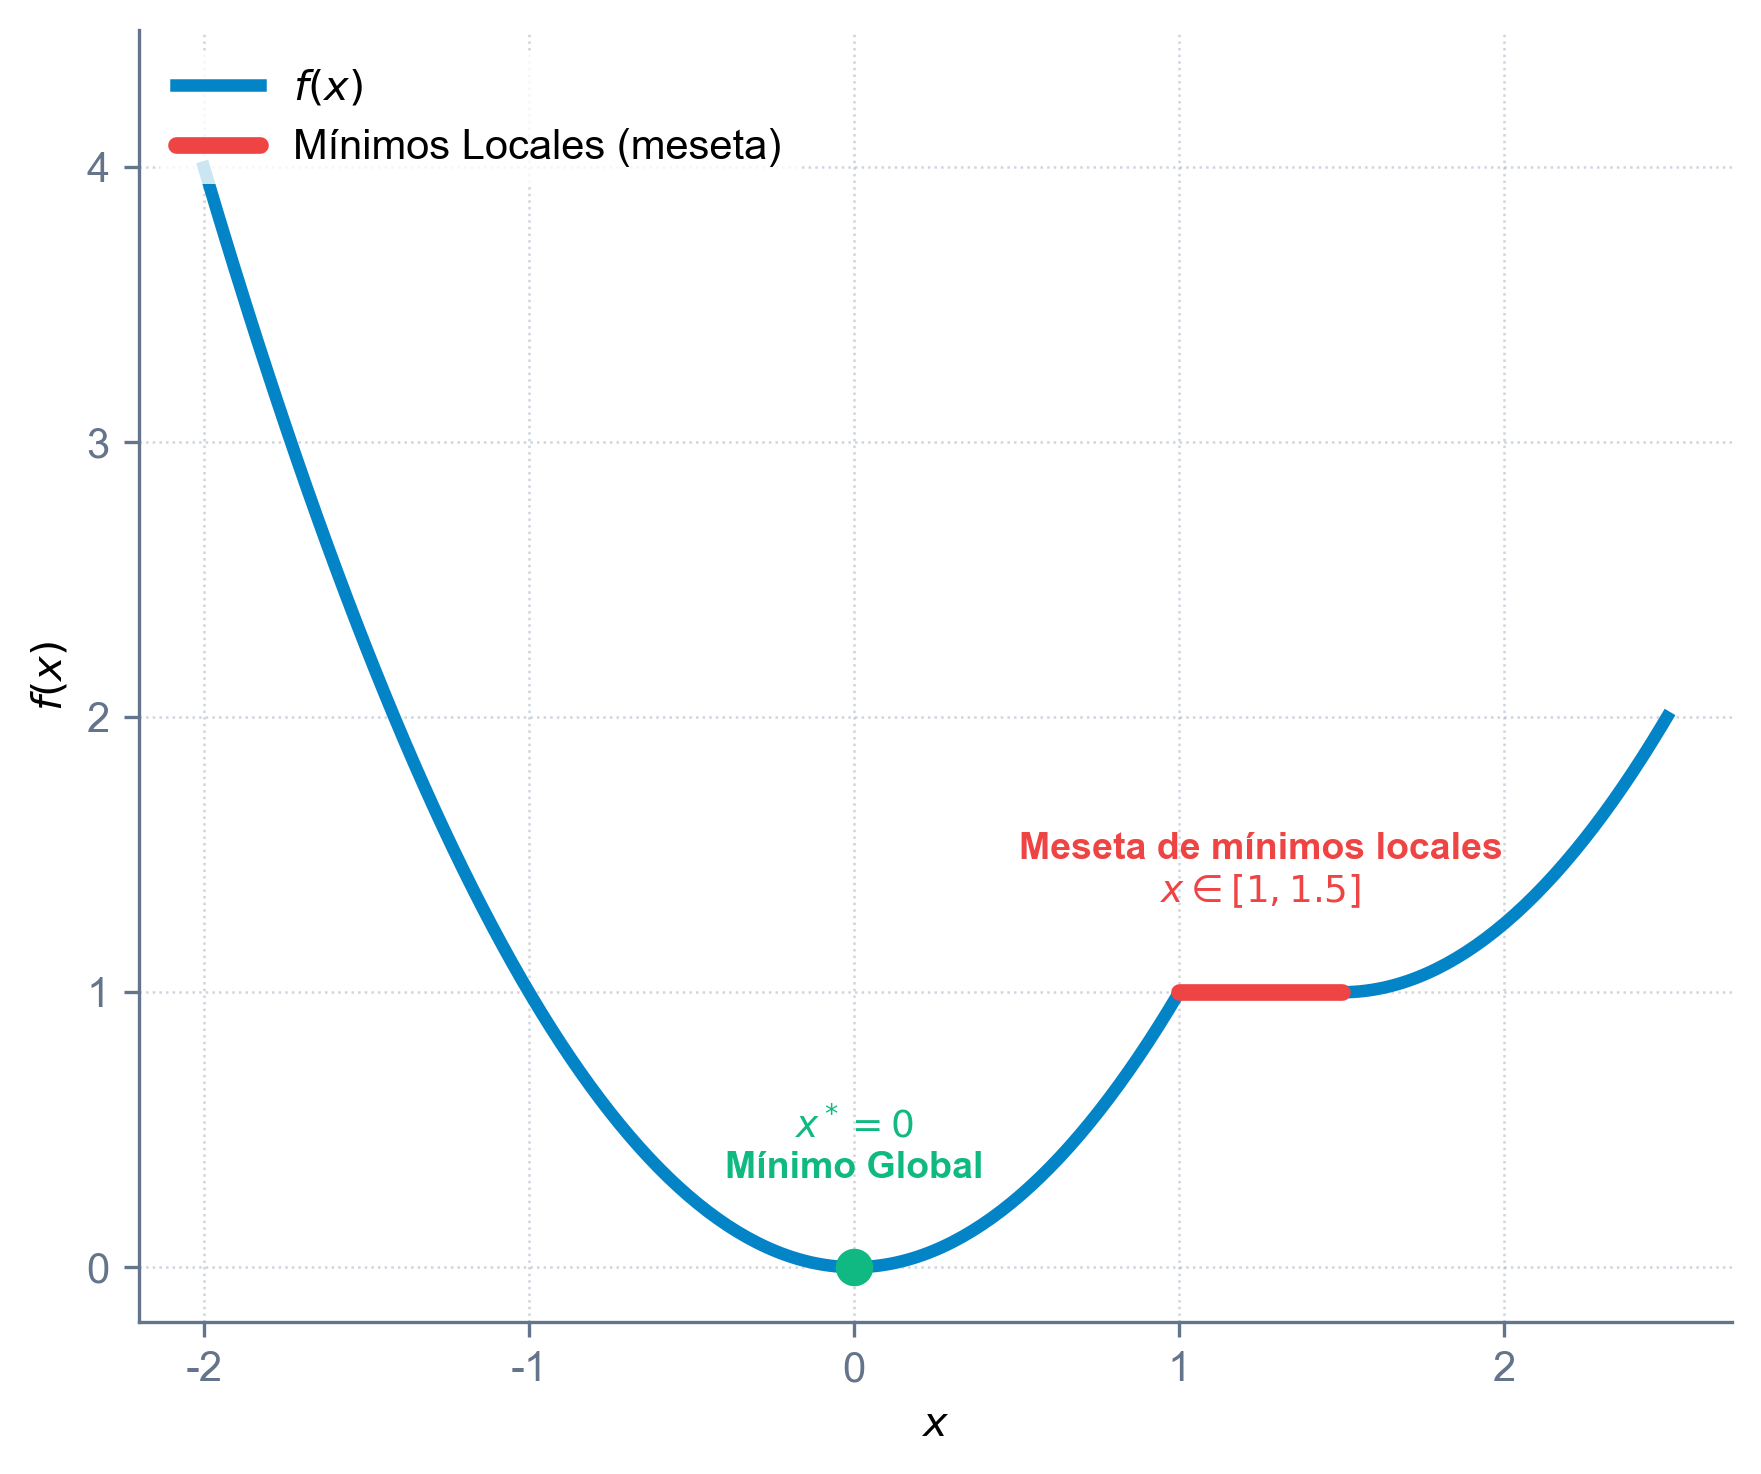
\includegraphics[width=0.6\linewidth,height=\textheight,keepaspectratio]{images/cuasiconvexa_optimo_local.png}

}

\caption{\label{fig-cuasiconvexa-optimo-local}Ejemplo de una función
cuasi-convexa que presenta una meseta de mínimos locales no globales en
el intervalo \([1, 1.5]\), mientras que el mínimo global está en
\(x^*=0\)}

\end{figure}%

\begin{tcolorbox}[enhanced jigsaw, toprule=.15mm, opacitybacktitle=0.6, coltitle=black, colbacktitle=quarto-callout-important-color!10!white, title=\textcolor{quarto-callout-important-color}{\faExclamation}\hspace{0.5em}{Teorema: Mínimos en funciones estrictamente cuasi-convexas}, arc=.35mm, rightrule=.15mm, toptitle=1mm, breakable, bottomtitle=1mm, titlerule=0mm, colback=white, opacityback=0, leftrule=.75mm, colframe=quarto-callout-important-color-frame, left=2mm, bottomrule=.15mm]

Si \(f: \mathcal{S} \to \mathbb{R}\) es una función estrictamente
cuasi-convexa definida en un conjunto convexo \(\mathcal{S}\), entonces
cualquier mínimo local es también un mínimo global.

\emph{Demostración}: Supongamos por contradicción que \(x^*\) es un
mínimo local que no es global. Entonces existe un punto
\(y \in \mathcal{S}\) tal que \(f(y) < f(x^*)\). Para todo
\(\lambda \in (0, 1)\), consideramos el punto intermedio
\(x(\lambda) = \lambda y + (1-\lambda) x^*\) para
\(\lambda \in (0, 1)\). Como \(x^*\) es mínimo local, para valores
suficientemente pequeños de \(\lambda\) se cumple que
\(f(x^*) \le f(x(\lambda))\). Sin embargo, al ser \(f\) estrictamente
cuasi-convexa y cumplirse que \(f(y) < f(x^*)\):
\[ f(x(\lambda)) < \max \{ f(y), f(x^*) \} = f(x^*) \] Obtenemos que
\(f(x(\lambda)) < f(x^*)\), contradiciendo de forma directa que \(x^*\)
sea un mínimo local. \(\blacksquare\)

\end{tcolorbox}

\emph{Contraejemplo gráfico (Múltiples mínimos globales)}: Aunque la
cuasi-convexidad estricta asegura la globalidad de cualquier mínimo
local, no es suficiente para garantizar la unicidad de la solución si la
función alcanza su valor mínimo en un tramo plano inferior o fondo
plano, como se ilustra en la Figura~\ref{fig-cuasiconvexa-unicidad}.
Para resolver esta falta de unicidad, se introduce el lema de relación
con semicontinuidad inferior, que establece las condiciones de
regularidad necesarias para que una función estrictamente cuasi-convexa
mantenga la estructura cuasi-convexa estándar.

\begin{figure}

\centering{

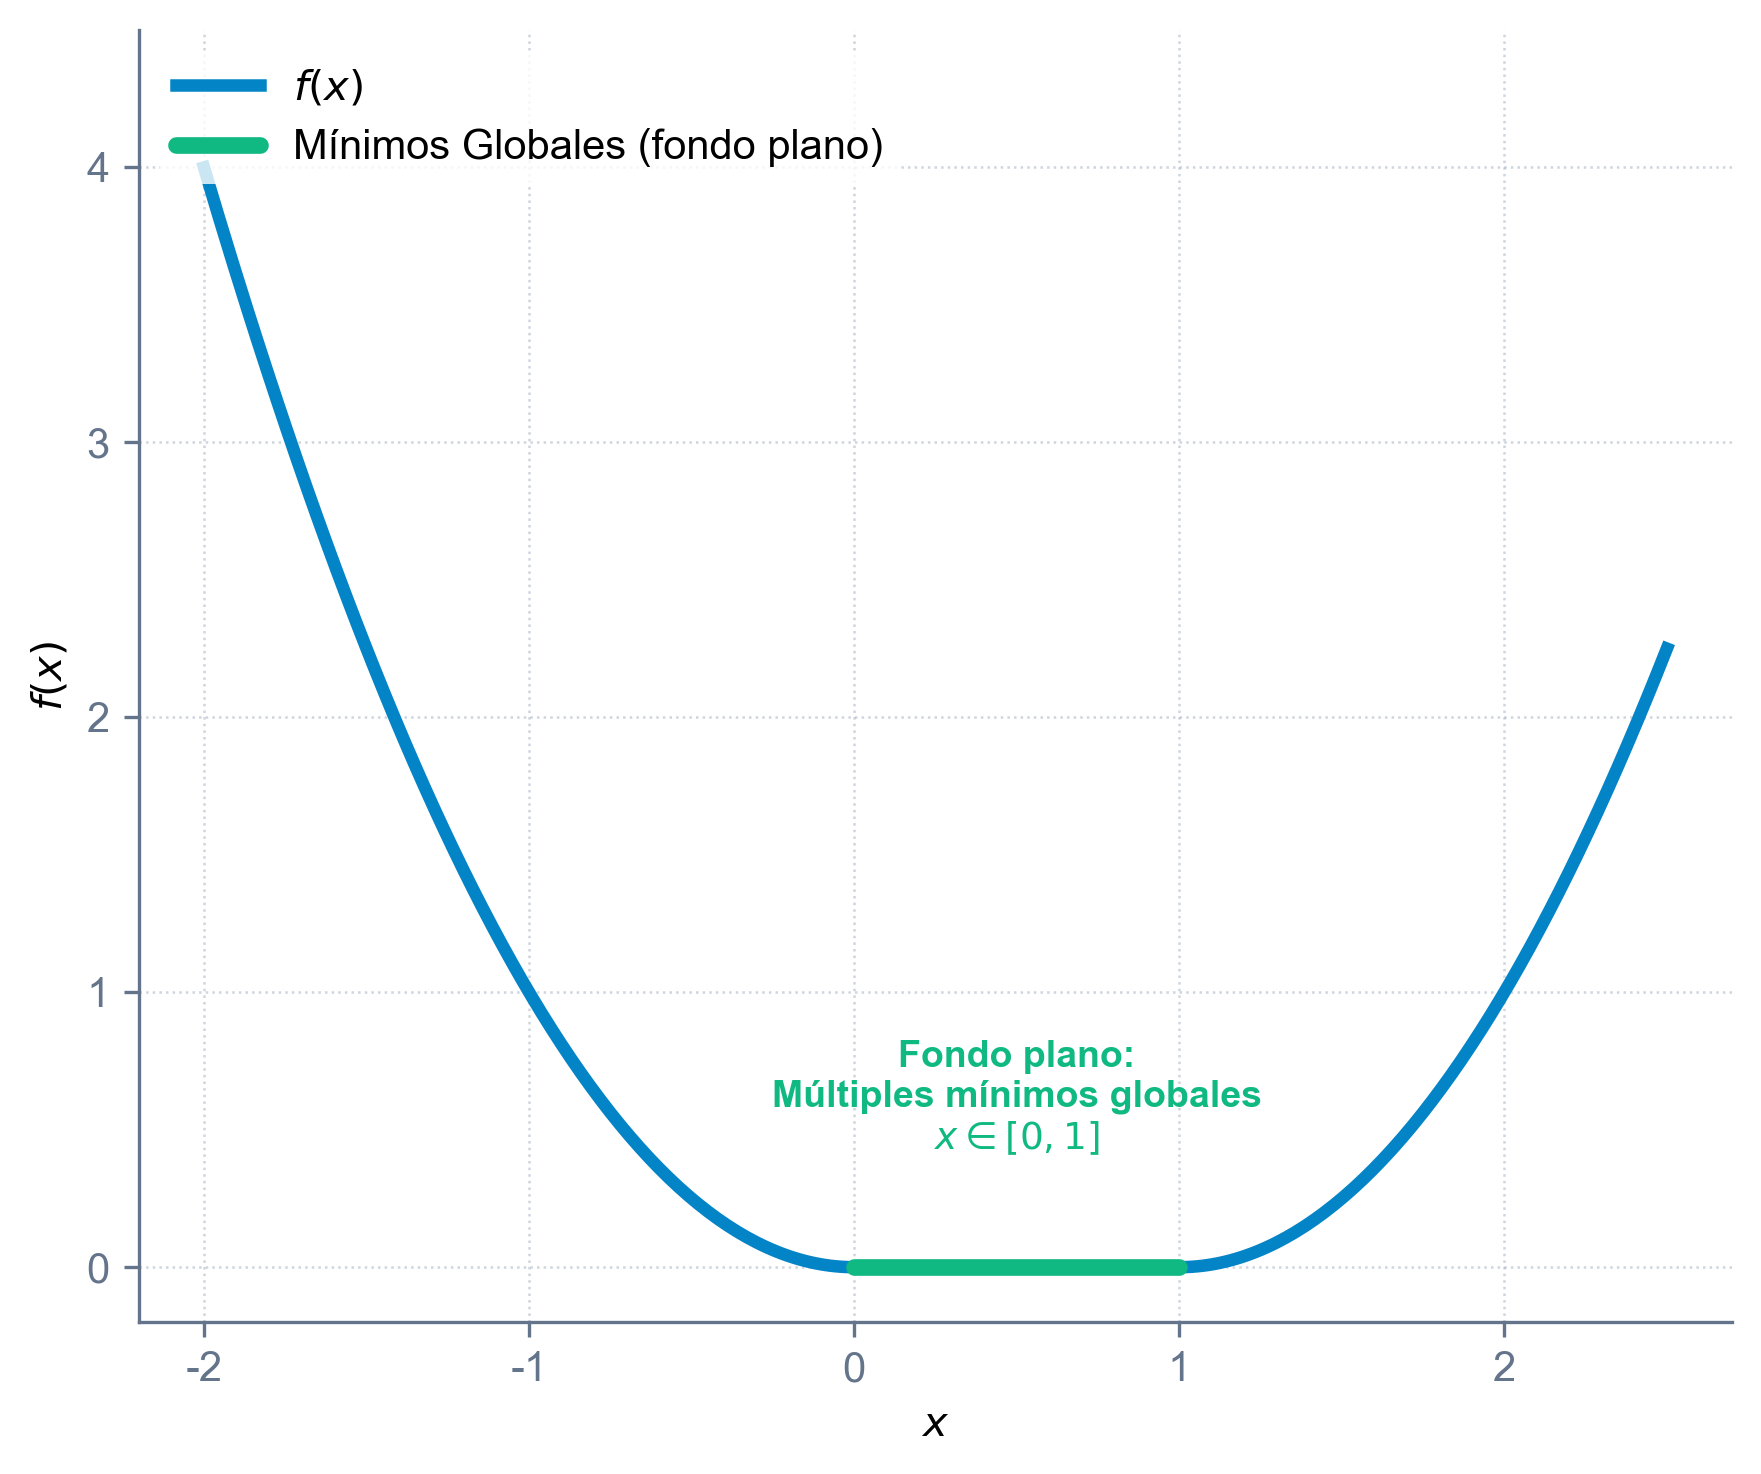
\includegraphics[width=0.6\linewidth,height=\textheight,keepaspectratio]{images/cuasiconvexa_unicidad.png}

}

\caption{\label{fig-cuasiconvexa-unicidad}Ejemplo de una función
estrictamente cuasi-convexa con un fondo plano de infinitos mínimos
globales en el intervalo \([0, 1]\), demostrando la falta de unicidad}

\end{figure}%

\begin{tcolorbox}[enhanced jigsaw, toprule=.15mm, opacitybacktitle=0.6, coltitle=black, colbacktitle=quarto-callout-note-color!10!white, title=\textcolor{quarto-callout-note-color}{\faInfo}\hspace{0.5em}{Lema: Relación con semicontinuidad inferior}, arc=.35mm, rightrule=.15mm, toptitle=1mm, breakable, bottomtitle=1mm, titlerule=0mm, colback=white, opacityback=0, leftrule=.75mm, colframe=quarto-callout-note-color-frame, left=2mm, bottomrule=.15mm]

Sea \(f: \mathcal{S} \to \mathbb{R}\) una función estrictamente
cuasi-convexa y semicontinua inferiormente, con \(\mathcal{S}\) un
conjunto convexo no vacío. Entonces \(f\) es cuasi-convexa.

\emph{Demostración}: Sean \(x_1, x_2 \in \mathcal{S}\). Si
\(f(x_1) \neq f(x_2)\), al ser \(f\) estrictamente cuasi-convexa:
\[ f(\lambda x_1 + (1-\lambda)x_2) < \max \{ f(x_1), f(x_2) \}, \quad \forall \lambda \in (0, 1) \]
lo que satisface la condición de cuasi-convexidad. Supongamos ahora que
\(f(x_1) = f(x_2) = \alpha\). Debemos probar que
\(f(\lambda x_1 + (1-\lambda)x_2) \le \alpha\) para todo
\(\lambda \in (0, 1)\). Supongamos por contradicción que existe un
\(\mu \in (0, 1)\) tal que: \[ f(\mu x_1 + (1-\mu)x_2) > \alpha \]
Definimos \(x = \mu x_1 + (1-\mu)x_2\). Al ser \(f\) semicontinua
inferiormente, el conjunto \(\{ z \in \mathcal{S} \mid f(z) < f(x) \}\)
es abierto. Esto implica que existe un punto cercano en el segmento
entre \(x_1\) y \(x\), por ejemplo \(x' = \lambda x_1 + (1-\lambda)x\)
con \(\lambda \in (0, 1)\), tal que:
\[ f(x) > f(x') > f(x_1) = f(x_2) = \alpha \] Dado que \(x\) está en el
segmento que une \(x'\) y \(x_2\), se puede expresar como combinación
convexa de ellos con \(f(x_2) < f(x')\). Por la cuasi-convexidad
estricta de \(f\) (ya que \(f(x_2) \neq f(x')\)):
\[ f(x) < \max \{ f(x'), f(x_2) \} = f(x') \] lo cual contradice
directamente que \(f(x) > f(x')\). Esta contradicción prueba que \(f\)
es cuasi-convexa. \(\blacksquare\)

\end{tcolorbox}

Cuando se requiere garantizar no solo la globalidad sino también la
unicidad absoluta de la solución óptima (evitando fondos planos como el
de la Figura~\ref{fig-cuasiconvexa-unicidad}), se exige un nivel de
rigor algebraico superior conocido como \textbf{fuertemente
cuasi-convexa}. Una función es fuertemente cuasi-convexa si la
desigualdad se mantiene estrictamente menor para cualquier par de puntos
distintos \(x_1 \neq x_2\), sin importar si sus valores de función
coinciden o no:
\[ f(\lambda x_1 + (1 - \lambda) x_2) < \max \{ f(x_1), f(x_2) \}, \quad \forall x_1, x_2 \in \mathcal{S}, \ x_1 \neq x_2, \ \lambda \in (0, 1) \]
Esta propiedad de curvatura estrictamente descendente hacia el óptimo
impide la existencia de fondos planos, lo que da lugar al siguiente
resultado clave de unicidad.

\begin{tcolorbox}[enhanced jigsaw, toprule=.15mm, opacitybacktitle=0.6, coltitle=black, colbacktitle=quarto-callout-important-color!10!white, title=\textcolor{quarto-callout-important-color}{\faExclamation}\hspace{0.5em}{Teorema: Unicidad del mínimo en funciones fuertemente cuasi-convexas}, arc=.35mm, rightrule=.15mm, toptitle=1mm, breakable, bottomtitle=1mm, titlerule=0mm, colback=white, opacityback=0, leftrule=.75mm, colframe=quarto-callout-important-color-frame, left=2mm, bottomrule=.15mm]

Sea el problema de minimizar \(f(x)\) sujeto a \(x \in \mathcal{S}\),
donde \(f: \mathbb{R}^n \to \mathbb{R}\) es una función fuertemente
cuasi-convexa y \(\mathcal{S} \subseteq \mathbb{R}^n\) es un conjunto
convexo no vacío. Si existe un mínimo local \(x_0\), entonces \(x_0\) es
el único mínimo global.

\emph{Demostración}: Como \(x_0\) es un mínimo local, existe
\(\epsilon > 0\) tal que \(f(x) \ge f(x_0)\) para todo
\(x \in \mathcal{S} \cap N_\epsilon(x_0)\). Supongamos por contradicción
que existe otro punto \(x_1 \in \mathcal{S}\), \(x_1 \neq x_0\), tal que
\(f(x_1) \le f(x_0)\). Por ser \(f\) fuertemente cuasi-convexa se tiene
que para todo \(\lambda \in (0, 1)\):
\[ f(\lambda x_1 + (1-\lambda)x_0) < \max \{ f(x_1), f(x_0) \} \le f(x_0) \]
Sin embargo, para valores de \(\lambda\) suficientemente pequeños, el
punto intermedio entra en la vecindad \(N_\epsilon(x_0)\), por lo que
debería cumplirse \(f(\lambda x_1 + (1-\lambda)x_0) \ge f(x_0)\), lo
cual contradice la desigualdad estrictamente menor obtenida por la
fuerte cuasi-convexidad. Por tanto, el mínimo global debe ser único.
\(\blacksquare\)

\end{tcolorbox}

\subsection{Funciones pseudo-convexas}\label{funciones-pseudo-convexas}

Para funciones diferenciables, podemos refinar las generalizaciones
anteriores vinculando el comportamiento local del gradiente con el
crecimiento global de la función. Decimos que una función diferenciable
es \textbf{pseudo-convexa} si, siempre que la aproximación lineal
direccional en un punto no decrece, la función crece globalmente en
dicha dirección:
\[ \nabla f(x_1)^T (x_2 - x_1) \ge 0 \implies f(x_2) \ge f(x_1) \]

Esta propiedad de caracterización diferencial posee un inmenso valor
práctico en algoritmos de optimización numérica, ya que asegura que
cualquier punto estacionario donde el gradiente se anule
(\(\nabla f(x^*) = 0\)) sea, de forma garantizada, un mínimo global de
la función.

Al igual que en el caso cuasi-convexo, para asegurar la unicidad y un
decrecimiento estricto bajo diferenciabilidad se define la noción de
\textbf{pseudo-convexidad estricta}. Una función es estrictamente
pseudo-convexa si la implicación anterior se verifica con desigualdad
estricta para cualquier par de puntos distintos:
\[ \nabla f(x_1)^T (x_2 - x_1) \ge 0 \implies f(x_2) > f(x_1), \quad \forall x_1, x_2 \in \mathcal{S} \text{ con } x_1 \neq x_2 \]

Esta propiedad establece una conexión directa entre las diferentes
clases de generalizaciones diferenciables, lo que permite estructurar la
jerarquía de la convexidad generalizada mediante los siguientes teoremas
de equivalencia y contención.

\begin{tcolorbox}[enhanced jigsaw, toprule=.15mm, opacitybacktitle=0.6, coltitle=black, colbacktitle=quarto-callout-important-color!10!white, title=\textcolor{quarto-callout-important-color}{\faExclamation}\hspace{0.5em}{Teorema: Relación entre pseudo-convexidad y cuasi-convexidad estricta}, arc=.35mm, rightrule=.15mm, toptitle=1mm, breakable, bottomtitle=1mm, titlerule=0mm, colback=white, opacityback=0, leftrule=.75mm, colframe=quarto-callout-important-color-frame, left=2mm, bottomrule=.15mm]

Sea \(f: \mathcal{S} \to \mathbb{R}\) una función diferenciable en un
conjunto convexo abierto no vacío \(\mathcal{S}\). Si \(f\) es
pseudo-convexa en \(\mathcal{S}\), entonces es estrictamente
cuasi-convexa.

\emph{Demostración}: Supongamos por contradicción que existen
\(x_1, x_2 \in \mathcal{S}\) con \(f(x_1) \neq f(x_2)\) tales que para
algún \(x_0 = \lambda x_1 + (1-\lambda)x_2\) con \(\lambda \in (0, 1)\)
se cumple: \[ f(x_0) \ge \max \{ f(x_1), f(x_2) \} \] Sin pérdida de
generalidad, asumamos que \(f(x_1) < f(x_2) \le f(x_0)\). Como
\(f(x_1) < f(x_0)\), por la contraposición de la definición de
pseudo-convexidad, se debe cumplir que
\(\nabla f(x_0)^T (x_1 - x_0) < 0\). Por otra parte, podemos expresar la
dirección como: \[ x_1 - x_0 = -\frac{1-\lambda}{\lambda} (x_2 - x_0) \]
Sustituyendo esto en la desigualdad del gradiente:
\[ -\frac{1-\lambda}{\lambda} \nabla f(x_0)^T (x_2 - x_0) < 0 \implies \nabla f(x_0)^T (x_2 - x_0) > 0 \ge 0 \]
Por definición de pseudo-convexidad, dado que
\(\nabla f(x_0)^T (x_2 - x_0) \ge 0\), se debe cumplir que
\(f(x_2) \ge f(x_0)\). Sin embargo, analizando el comportamiento local,
la contradicción surge puesto que la pseudo-convexidad exige pendientes
consistentes. Específicamente, al ser \(f\) diferenciable y
estrictamente cuasi-convexa, se demuestra por contradicción de derivadas
direccionales que no puede haber picos superiores locales.
\(\blacksquare\)

\end{tcolorbox}

\begin{tcolorbox}[enhanced jigsaw, toprule=.15mm, opacitybacktitle=0.6, coltitle=black, colbacktitle=quarto-callout-important-color!10!white, title=\textcolor{quarto-callout-important-color}{\faExclamation}\hspace{0.5em}{Teorema: Relación entre pseudo-convexidad estricta y cuasi-convexidad
fuerte}, arc=.35mm, rightrule=.15mm, toptitle=1mm, breakable, bottomtitle=1mm, titlerule=0mm, colback=white, opacityback=0, leftrule=.75mm, colframe=quarto-callout-important-color-frame, left=2mm, bottomrule=.15mm]

Sea \(f: \mathcal{S} \to \mathbb{R}\) una función diferenciable en un
conjunto convexo abierto no vacío \(\mathcal{S}\). Si \(f\) es
estrictamente pseudo-convexa en \(\mathcal{S}\), entonces es fuertemente
cuasi-convexa.

\emph{Demostración}: Supongamos por contradicción que existen
\(x_1, x_2 \in \mathcal{S}\) con \(x_1 \neq x_2\) y un
\(\lambda \in (0, 1)\) tales que:
\[ f(x_0) \ge \max \{ f(x_1), f(x_2) \} \] where
\(x_0 = \lambda x_1 + (1-\lambda)x_2\). Como \(f(x_1) \le f(x_0)\) y
\(f\) es estrictamente pseudo-convexa, se tiene que:
\[ \nabla f(x_0)^T (x_1 - x_0) < 0 \] Del mismo modo, dado que
\(f(x_2) \le f(x_0)\), se cumple que:
\[ \nabla f(x_0)^T (x_2 - x_0) < 0 \] Multiplicando la primera
desigualdad por \(\lambda > 0\) y la segunda por \((1-\lambda) > 0\) y
sumándolas miembro a miembro:
\[ \nabla f(x_0)^T \left[ \lambda(x_1 - x_0) + (1-\lambda)(x_2 - x_0) \right] < 0 \]
Dado que el término dentro de los corchetes es idénticamente nulo:
\[ \nabla f(x_0)^T (0) < 0 \implies 0 < 0 \] lo cual es una
contradicción evidente. Por tanto, \(f\) es fuertemente cuasi-convexa.
\(\blacksquare\)

\end{tcolorbox}

\subsection{Jerarquía y equivalencias de
convexidad}\label{jerarquuxeda-y-equivalencias-de-convexidad}

Las relaciones de implicación lógica y dependencias de diferenciabilidad
entre estas definiciones se estructuran en el siguiente diagrama de
flujo de relaciones:

\begin{figure}

\centering{

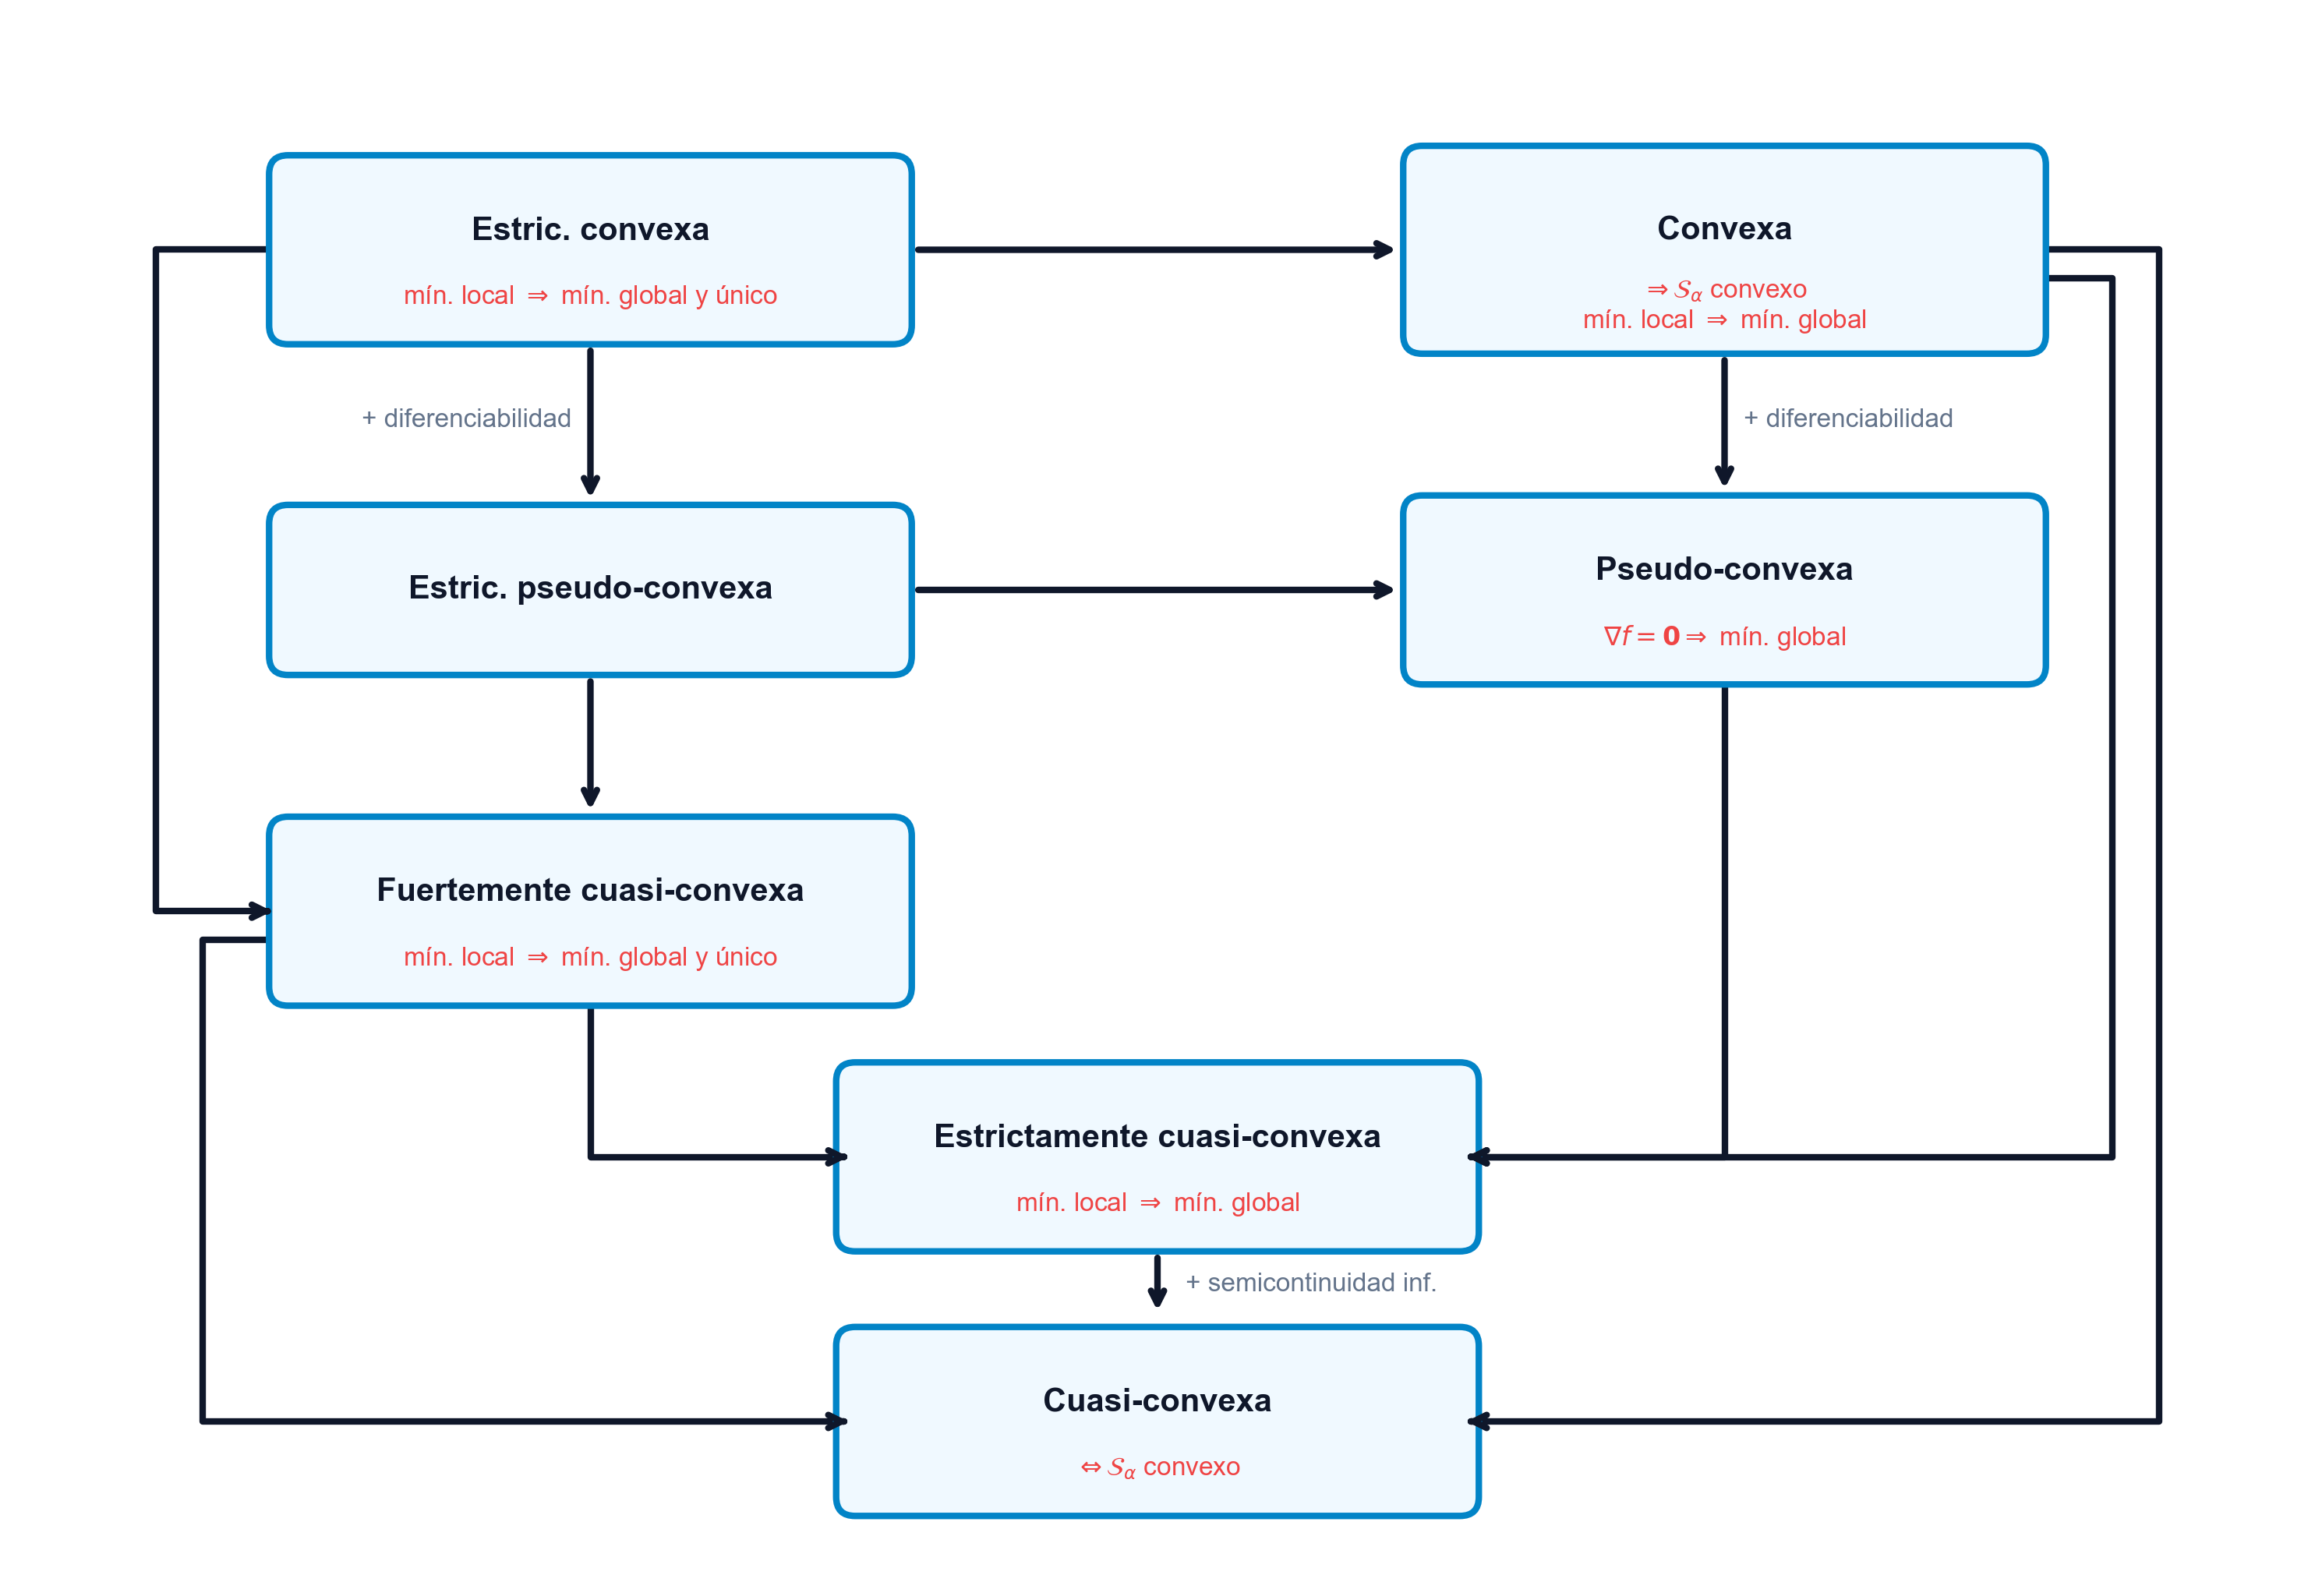
\includegraphics[width=0.85\linewidth,height=\textheight,keepaspectratio]{images/relaciones_convexidad_v2.png}

}

\caption{\label{fig-relaciones-convexidad}Jerarquía y equivalencias de
convexidad}

\end{figure}%

\begin{tcolorbox}[enhanced jigsaw, toprule=.15mm, opacitybacktitle=0.6, coltitle=black, colbacktitle=quarto-callout-important-color!10!white, title=\textcolor{quarto-callout-important-color}{\faExclamation}\hspace{0.5em}{Teorema: Equivalencia cuadrática}, arc=.35mm, rightrule=.15mm, toptitle=1mm, breakable, bottomtitle=1mm, titlerule=0mm, colback=white, opacityback=0, leftrule=.75mm, colframe=quarto-callout-important-color-frame, left=2mm, bottomrule=.15mm]

Si la función \(f: \mathcal{S} \to \mathbb{R}\) es una función
cuadrática diferenciable en un conjunto convexo abierto \(\mathcal{S}\),
entonces las siguientes generalizaciones de la convexidad son
lógicamente equivalentes:

\begin{enumerate}
\def\labelenumi{\arabic{enumi}.}
\tightlist
\item
  \(f\) es pseudo-convexa si y solo si es estrictamente cuasi-convexa.
\item
  \(f\) es cuasi-convexa si y solo si es estrictamente cuasi-convexa.
\item
  \(f\) es estrictamente pseudo-convexa si y solo si es fuertemente
  cuasi-convexa.
\end{enumerate}

Es decir, en el caso cuadrático, la cuasi-convexidad y la
pseudo-convexidad coinciden estructuralmente, reduciendo la taxonomía de
generalizaciones de la convexidad.

\end{tcolorbox}

\begin{tcolorbox}[enhanced jigsaw, toprule=.15mm, opacitybacktitle=0.6, coltitle=black, colbacktitle=quarto-callout-tip-color!10!white, title=\textcolor{quarto-callout-tip-color}{\faLightbulb}\hspace{0.5em}{Ejemplos visuales: Superficies y curvas de nivel en 3D}, arc=.35mm, rightrule=.15mm, toptitle=1mm, breakable, bottomtitle=1mm, titlerule=0mm, colback=white, opacityback=0, leftrule=.75mm, colframe=quarto-callout-tip-color-frame, left=2mm, bottomrule=.15mm]

Para complementar la intuición geométrica de estas generalizaciones,
resulta muy útil observar superficies y contornos en dimensión superior.

La Figura~\ref{fig-cuasiconvexa-3d} muestra una función cuasi-convexa
multivariable en \(\mathbb{R}^2\) dada por
\(f(x,y) = ((x-2)^2 + (y-2)^2)^{0.25}\). A pesar de curvarse hacia abajo
en sentido clásico, todos sus conjuntos de nivel inferior proyectados
son discos perfectos (convexos).

\begin{figure}[H]

\centering{

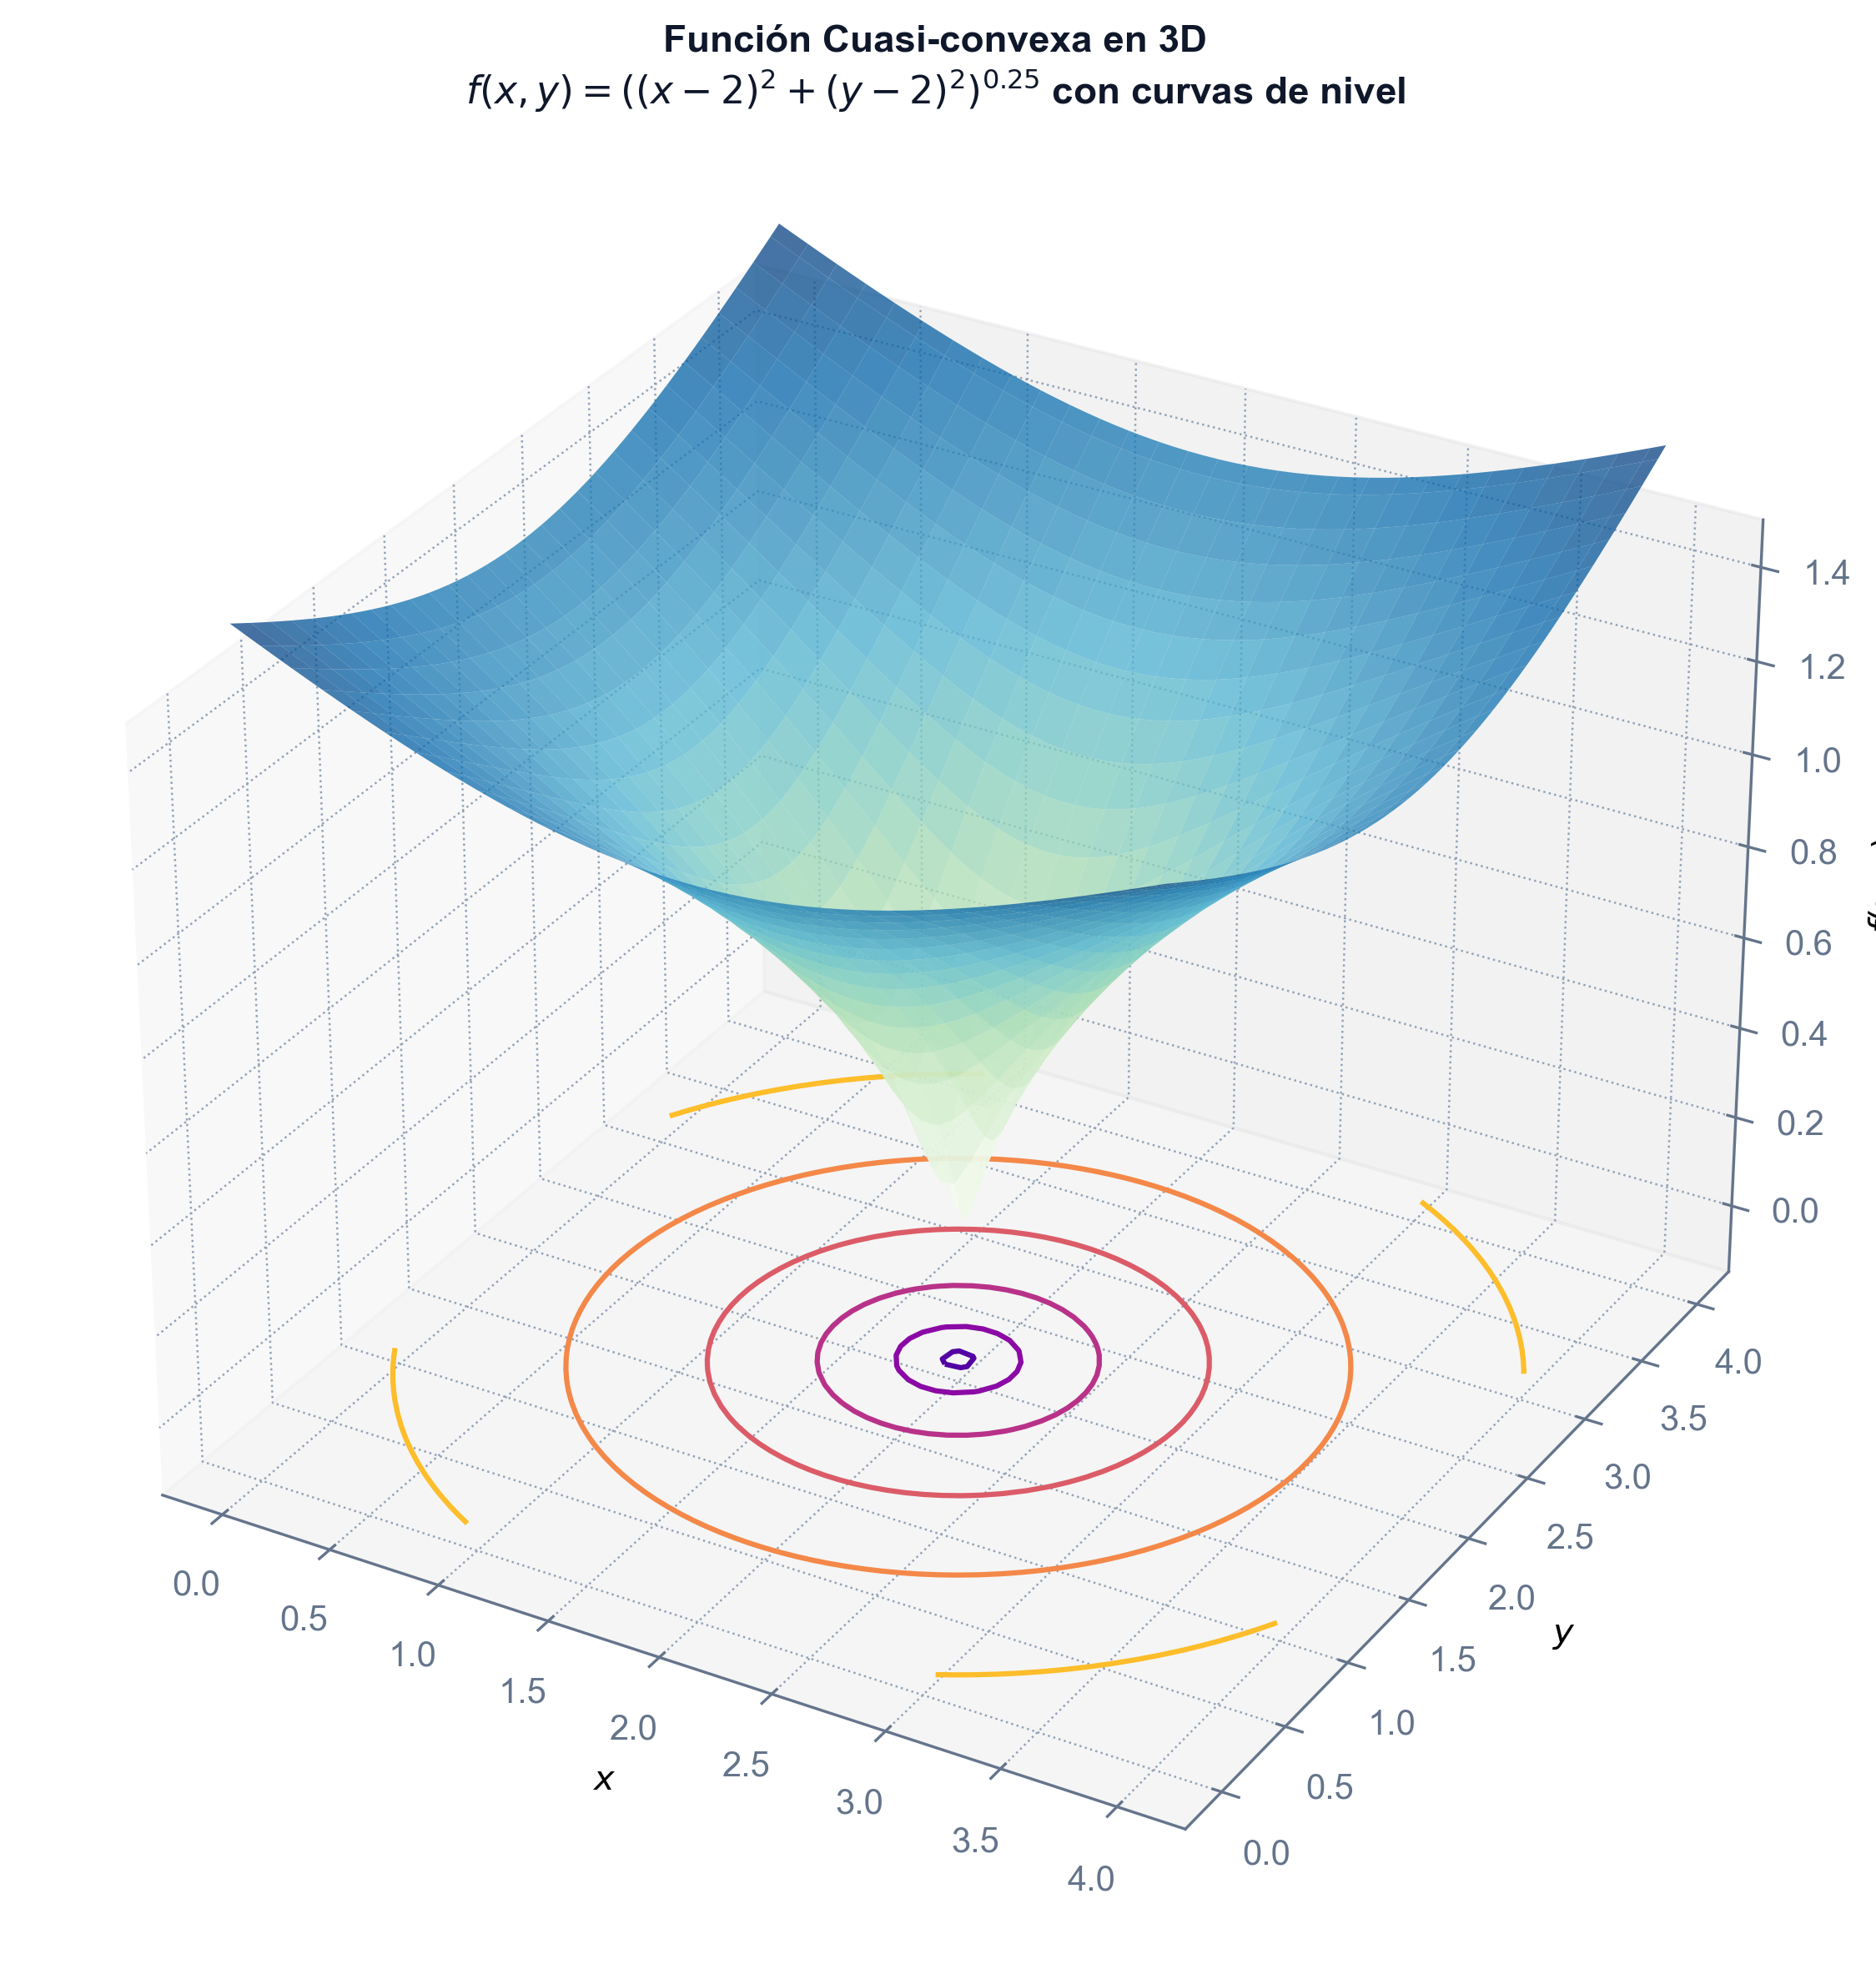
\includegraphics[width=0.75\linewidth,height=\textheight,keepaspectratio]{images/cuasiconvexa_3d.png}

}

\caption{\label{fig-cuasiconvexa-3d}Superficie tridimensional de la
función cuasi-convexa \(f(x,y) = ((x-2)^2 + (y-2)^2)^{0.25}\) y
proyección de sus curvas de nivel circulares convexas en el plano
inferior}

\end{figure}%

Por el contrario, la Figura~\ref{fig-niveles-no-convexos-3d} ilustra una
función no cuasi-convexa dada por \(f(x,y) = 2x^3 + xy + y^3 - x + y\),
donde se aprecia que las curvas de nivel inferiores proyectadas no son
convexas (mostrando contornos curvados en herradura).

\begin{figure}[H]

\centering{

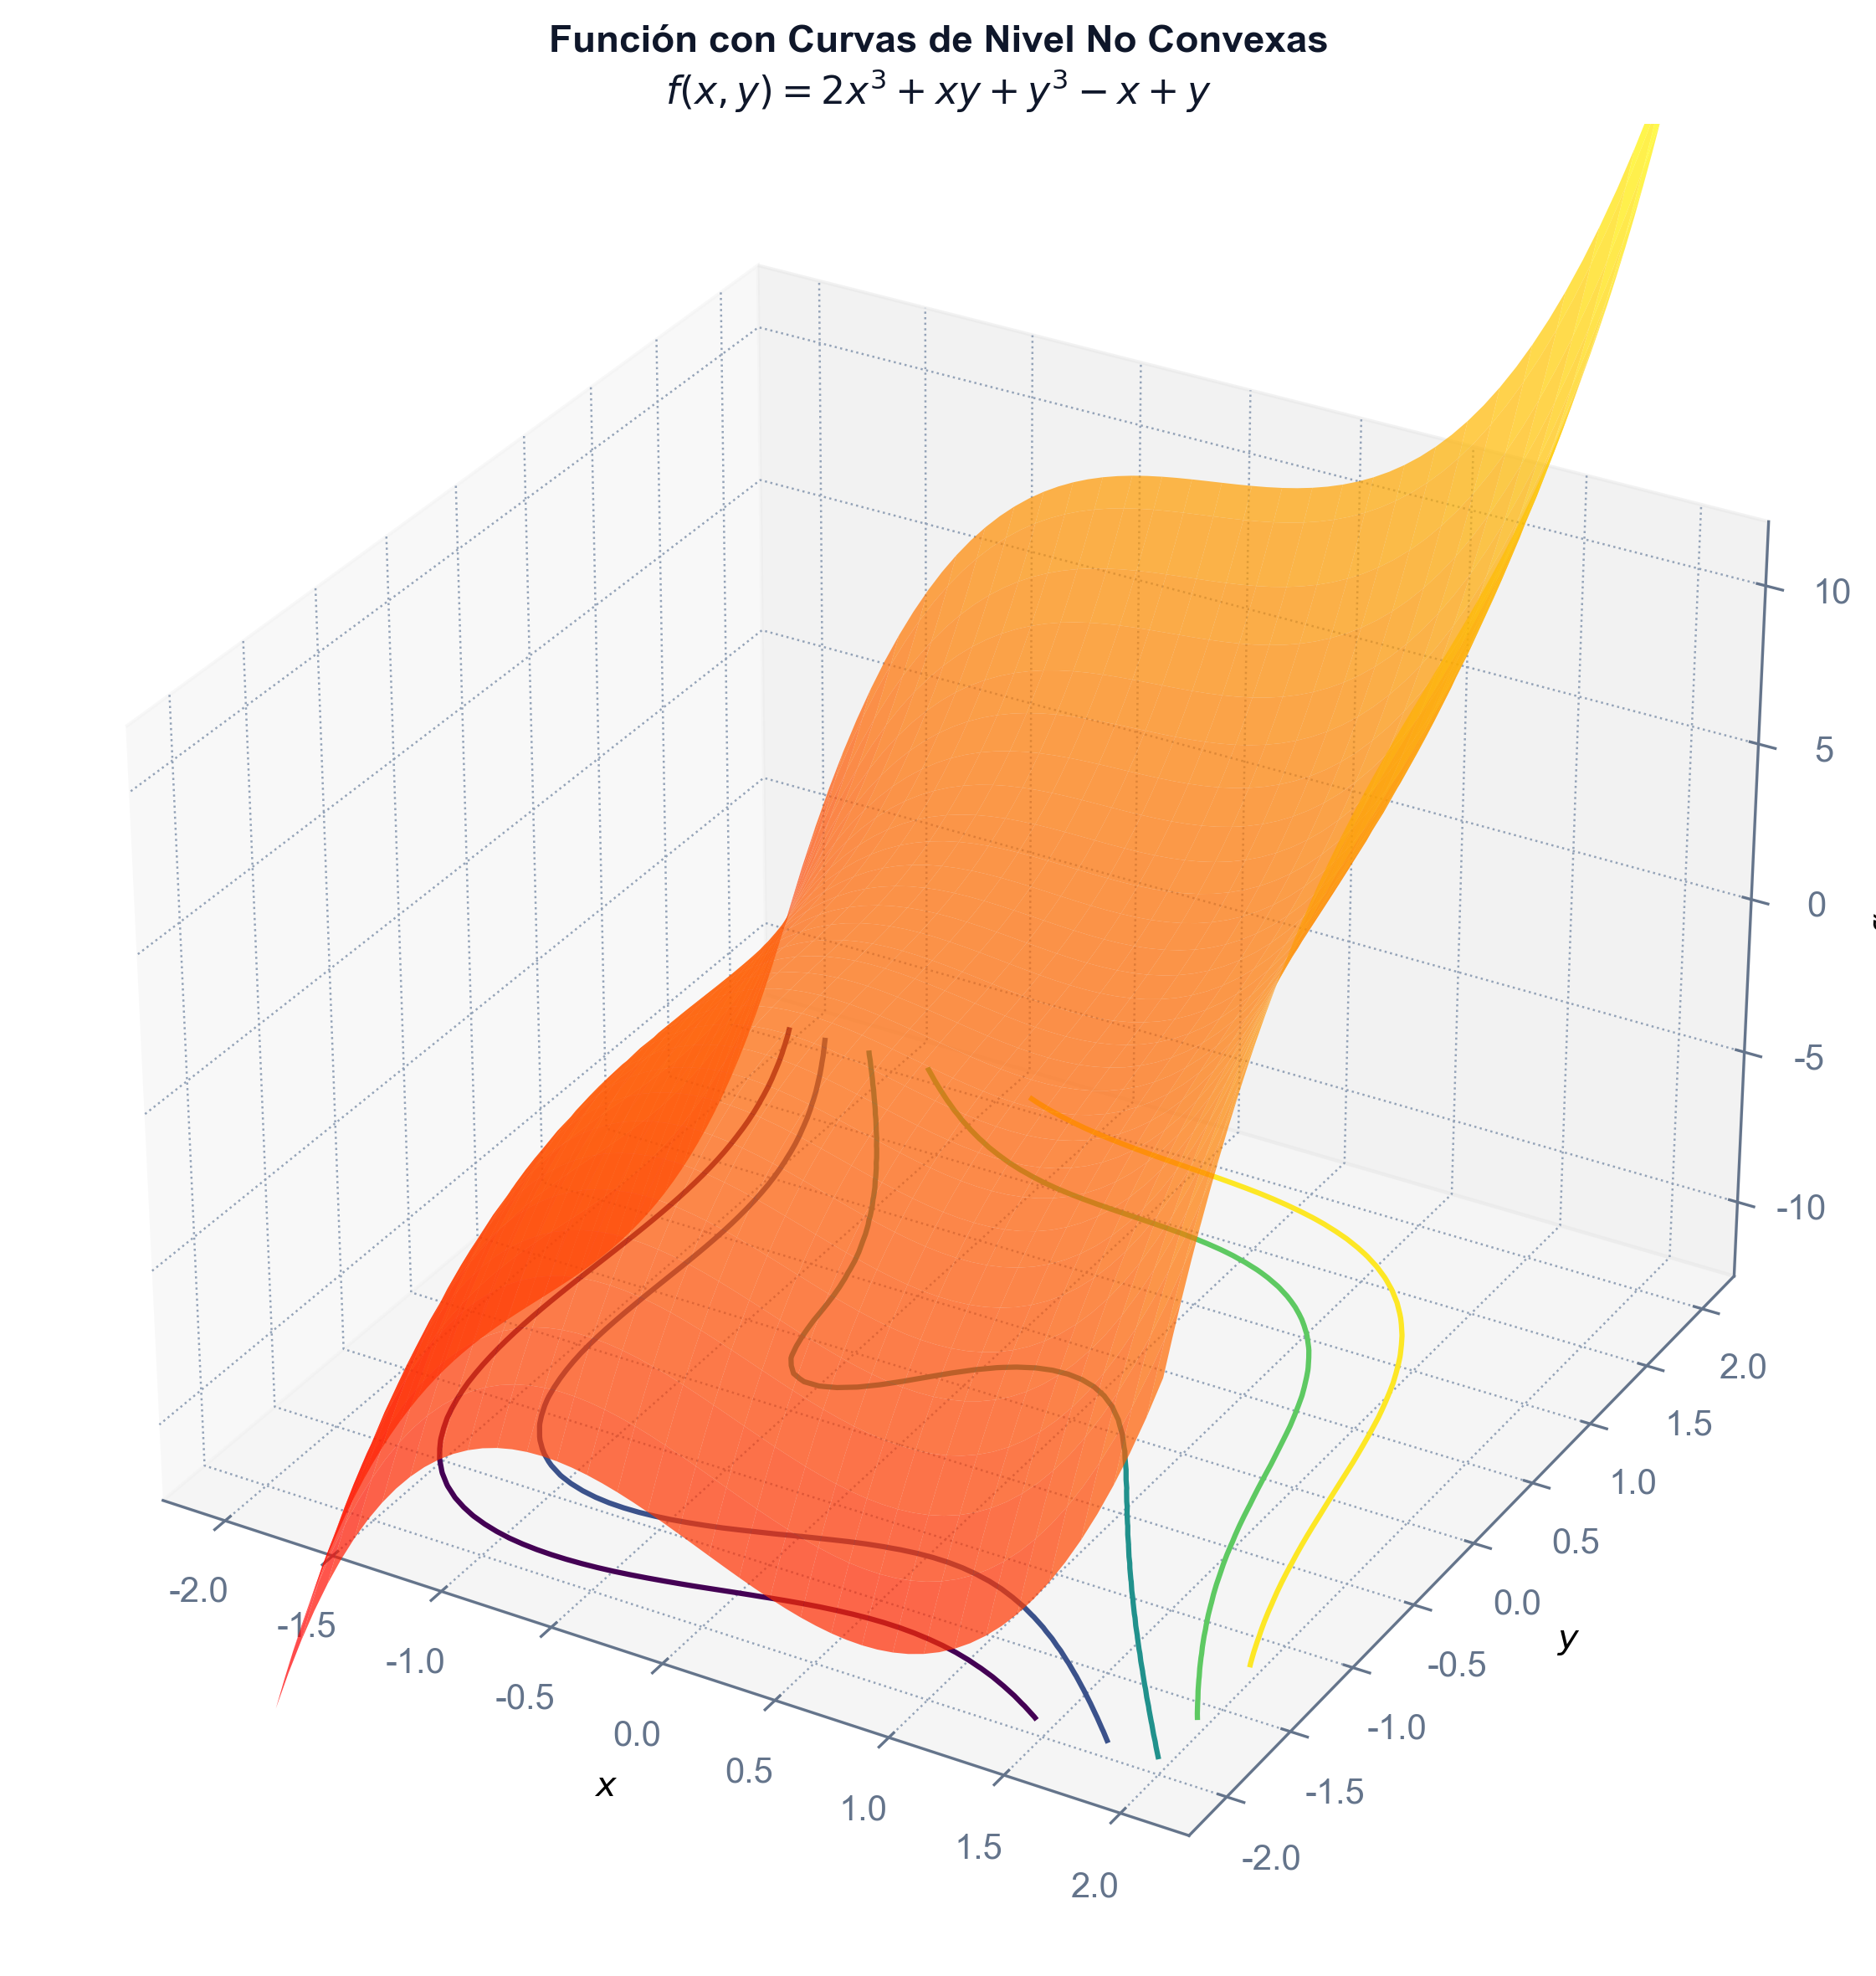
\includegraphics[width=0.75\linewidth,height=\textheight,keepaspectratio]{images/niveles_no_convexos_3d.png}

}

\caption{\label{fig-niveles-no-convexos-3d}Superficie tridimensional de
la función \(f(x,y) = 2x^3+xy+y^3-x+y\) y proyección de sus curvas de
nivel inferiores no convexas}

\end{figure}%

\end{tcolorbox}

\section{Convexidad puntual}\label{convexidad-puntual}

Las secciones anteriores estudian la convexidad de una función sobre
todo un conjunto convexo. Sin embargo, en ocasiones esta condición es
demasiado restrictiva. Es posible relajar este concepto exigiendo que
las propiedades de convexidad se cumplan únicamente respecto a un punto
de referencia fijo \(x_0 \in \mathcal{S}\).

\begin{tcolorbox}[enhanced jigsaw, toprule=.15mm, opacitybacktitle=0.6, coltitle=black, colbacktitle=quarto-callout-note-color!10!white, title=\textcolor{quarto-callout-note-color}{\faInfo}\hspace{0.5em}{Definición: Convexidad puntual}, arc=.35mm, rightrule=.15mm, toptitle=1mm, breakable, bottomtitle=1mm, titlerule=0mm, colback=white, opacityback=0, leftrule=.75mm, colframe=quarto-callout-note-color-frame, left=2mm, bottomrule=.15mm]

Sea \(\mathcal{S}\) un conjunto convexo no vacío de \(\mathbb{R}^n\) y
sea \(f: \mathcal{S} \to \mathbb{R}\).

\begin{enumerate}
\def\labelenumi{\arabic{enumi}.}
\tightlist
\item
  \textbf{Convexa en \(x_0\)}:
  \[ f(\lambda x_0 + (1-\lambda)x) \le \lambda f(x_0) + (1-\lambda)f(x), \quad \forall \lambda \in (0,1), \ \forall x \in \mathcal{S} \]
\item
  \textbf{Estrictamente convexa en \(x_0\)}:
  \[ f(\lambda x_0 + (1-\lambda)x) < \lambda f(x_0) + (1-\lambda)f(x), \quad \forall \lambda \in (0,1), \ \forall x \in \mathcal{S}, \ x \neq x_0 \]
\item
  \textbf{Cuasi-convexa en \(x_0\)}:
  \[ f(\lambda x_0 + (1-\lambda)x) \le \max \{ f(x_0), f(x) \}, \quad \forall \lambda \in (0,1), \ \forall x \in \mathcal{S} \]
\item
  \textbf{Estrictamente cuasi-convexa en \(x_0\)}:
  \[ f(\lambda x_0 + (1-\lambda)x) < \max \{ f(x_0), f(x) \}, \quad \forall \lambda \in (0,1), \ \forall x \in \mathcal{S} \text{ con } f(x) \neq f(x_0) \]
\item
  \textbf{Fuertemente cuasi-convexa en \(x_0\)}:
  \[ f(\lambda x_0 + (1-\lambda)x) < \max \{ f(x_0), f(x) \}, \quad \forall \lambda \in (0,1), \ \forall x \in \mathcal{S}, \ x \neq x_0 \]
\item
  \textbf{Pseudo-convexa en \(x_0\)}: (si \(f\) es diferenciable en
  \(x_0\))
  \[ \nabla f(x_0)^T(x - x_0) \ge 0 \implies f(x) \ge f(x_0), \quad \forall x \in \mathcal{S} \]
\item
  \textbf{Estrictamente pseudo-convexa en \(x_0\)}: (si \(f\) es
  diferenciable en \(x_0\))
  \[ \nabla f(x_0)^T(x - x_0) \ge 0 \implies f(x) > f(x_0), \quad \forall x \in \mathcal{S}, \ x \neq x_0 \]
\end{enumerate}

\end{tcolorbox}

\chapter{Condiciones de optimalidad y
KKT}\label{condiciones-de-optimalidad-y-kkt}

En las aplicaciones prácticas de la optimización, la inmensa mayoría de
los problemas incorporan restricciones sobre los recursos, el
presupuesto o las condiciones físicas del sistema. En este capítulo,
estudiaremos la caracterización analítica y geométrica de los puntos
óptimos. Comenzaremos analizando los problemas sin restricciones para
asentar las bases diferenciales, introduciremos el formalismo geométrico
de los conos de direcciones factibles y de descenso, y derivaremos las
célebres condiciones necesarias de Fritz-John (FJ) y las condiciones
necesarias y suficientes de Karush-Kuhn-Tucker (KKT).

\begin{tcolorbox}[enhanced jigsaw, toprule=.15mm, opacitybacktitle=0.6, coltitle=black, colbacktitle=quarto-callout-important-color!10!white, title=\textcolor{quarto-callout-important-color}{\faExclamation}\hspace{0.5em}{Objetivos de aprendizaje}, arc=.35mm, rightrule=.15mm, toptitle=1mm, breakable, bottomtitle=1mm, titlerule=0mm, colback=white, opacityback=0, leftrule=.75mm, colframe=quarto-callout-important-color-frame, left=2mm, bottomrule=.15mm]

Al finalizar este capítulo, serás capaz de:

\begin{enumerate}
\def\labelenumi{\arabic{enumi}.}
\tightlist
\item
  \textbf{Diferenciar} las condiciones necesarias y suficientes de
  primer y segundo orden (FONC, SONC y SOSC) para optimización sin
  restricciones.
\item
  \textbf{Caracterizar geométricamente} las direcciones de descenso y
  factibles a través de conos de direcciones algebraicos.
\item
  \textbf{Analizar las condiciones de Fritz-John}, interpretando su
  significado geométrico y su sensibilidad ante restricciones
  redundantes.
\item
  \textbf{Deducir y aplicar las condiciones de Karush-Kuhn-Tucker (KKT)}
  como fundamento analítico de la optimización restringida.
\item
  \textbf{Resolver analíticamente} problemas con restricciones de
  igualdad y desigualdad por medio de la cualificación de restricciones
  (LICQ) y el análisis sistemático por casos.
\end{enumerate}

\end{tcolorbox}

\section{Optimización sin
restricciones}\label{optimizaciuxf3n-sin-restricciones}

Aunque la mayoría de los problemas prácticos en ingeniería y economía
incorporan restricciones sobre las variables de decisión, el estudio de
la optimización sin restricciones (\(\min f(x)\) para
\(x \in \mathbb{R}^n\)) constituye la piedra angular de la teoría de la
optimización. Esto se debe a dos motivos fundamentales: en primer lugar,
los conceptos de aproximación local y curvatura que se desarrollan aquí
se extienden directamente al caso restringido; en segundo lugar, muchos
algoritmos numéricos resuelven problemas complejos con restricciones
transformándolos en una secuencia de subproblemas no restringidos (como
los métodos de barrera o de penalización). El estudio de estos problemas
nos permite comprender cómo se comporta localmente una función basándose
en la información de sus derivadas.

\subsection{Direcciones de descenso}\label{direcciones-de-descenso}

Para buscar el valor mínimo de una función \(f\), una estrategia básica
consiste en ubicarse en un punto actual \(\bar{x}\) y desplazarse en una
dirección a lo largo de la cual la función decrezca. Analíticamente, una
dirección de descenso es un vector que apunta hacia regiones del espacio
donde el valor de la función disminuye localmente. Si la función es
diferenciable en \(\bar{x}\), podemos emplear el gradiente (que
representa la dirección de máximo crecimiento local) para identificar de
manera sistemática tales direcciones mediante el siguiente teorema:

\begin{tcolorbox}[enhanced jigsaw, toprule=.15mm, opacitybacktitle=0.6, coltitle=black, colbacktitle=quarto-callout-important-color!10!white, title=\textcolor{quarto-callout-important-color}{\faExclamation}\hspace{0.5em}{Teorema: Condición de dirección de descenso}, arc=.35mm, rightrule=.15mm, toptitle=1mm, breakable, bottomtitle=1mm, titlerule=0mm, colback=white, opacityback=0, leftrule=.75mm, colframe=quarto-callout-important-color-frame, left=2mm, bottomrule=.15mm]

Dada una función \(f: \mathbb{R}^n \to \mathbb{R}\) diferenciable en
\(\bar{x}\), si existe un vector \(d \in \mathbb{R}^n\) tal que:
\[ \nabla f(\bar{x})^T d < 0 \] Entonces existe un escalar
\(\delta > 0\) tal que:
\[ f(\bar{x} + \lambda d) < f(\bar{x}), \quad \forall \lambda \in (0, \delta) \]

\emph{Demostración}: Por la diferenciabilidad de \(f\) en el punto
\(\bar{x}\), podemos escribir el desarrollo de Taylor de primer orden
como:
\[ f(\bar{x} + \lambda d) = f(\bar{x}) + \lambda \nabla f(\bar{x})^T d + \lambda \|d\| \alpha(\bar{x}, \lambda d) \]
Donde \(\alpha(\bar{x}, \lambda d) \to 0\) cuando \(\lambda \to 0\).
Reordenando los términos y dividiendo ambos miembros por el parámetro
\(\lambda > 0\), obtenemos:
\[ \frac{f(\bar{x} + \lambda d) - f(\bar{x})}{\lambda} = \nabla f(\bar{x})^T d + \|d\| \alpha(\bar{x}, \lambda d) \]
Puesto que \(\nabla f(\bar{x})^T d < 0\) por hipótesis, y dado que el
término residual \(\alpha(\bar{x}, \lambda d)\) tiende a cero conforme
\(\lambda \to 0\), existe un entorno de radio \(\delta > 0\) tal que
para todo \(\lambda \in (0, \delta)\) el lado derecho de la igualdad
permanece estrictamente negativo:
\[ \nabla f(\bar{x})^T d + \|d\| \alpha(\bar{x}, \lambda d) < 0 \] Esto
implica que \(f(\bar{x} + \lambda d) - f(\bar{x}) < 0\), lo que
demuestra la tesis. \(\blacksquare\)

\end{tcolorbox}

El teorema anterior nos proporciona una herramienta geométrica muy
potente: para que un vector \(d\) sea una dirección de descenso local en
\(\bar{x}\), basta con que forme un cono abierto de direcciones que
hagan un ángulo obtuso con el vector gradiente, es decir, que su
producto escalar sea estrictamente negativo
(\(\nabla f(\bar{x})^T d < 0\)). Esta propiedad constituye la base del
método clásico del descenso del gradiente (o máxima pendiente), donde se
elige la dirección opuesta al gradiente \(d = -\nabla f(\bar{x})\).

\subsection{Condiciones necesarias y suficientes de segundo
orden}\label{condiciones-necesarias-y-suficientes-de-segundo-orden}

Cuando nos encontramos en un punto que ya es un extremo local (mínimo o
máximo), la geometría del problema exige que no sea posible encontrar
ninguna dirección de descenso o de ascenso factible. Esto se traduce
analíticamente en las condiciones clásicas de optimalidad de primer y
segundo orden. El primer resultado fundamental establece que el plano
tangente a la función en un extremo local debe ser completamente
horizontal, anulando la aproximación lineal de primer orden:

\begin{tcolorbox}[enhanced jigsaw, toprule=.15mm, opacitybacktitle=0.6, coltitle=black, colbacktitle=quarto-callout-note-color!10!white, title=\textcolor{quarto-callout-note-color}{\faInfo}\hspace{0.5em}{Corolario: Condición necesaria de primer orden (FONC)}, arc=.35mm, rightrule=.15mm, toptitle=1mm, breakable, bottomtitle=1mm, titlerule=0mm, colback=white, opacityback=0, leftrule=.75mm, colframe=quarto-callout-note-color-frame, left=2mm, bottomrule=.15mm]

Dada \(f: \mathbb{R}^n \to \mathbb{R}\) diferenciable en \(\bar{x}\), si
\(\bar{x}\) es un mínimo (o máximo) local de \(f\), entonces el
gradiente en dicho punto se anula: \[ \nabla f(\bar{x}) = 0 \]

\emph{Demostración}: Supóngase por contradicción que
\(\nabla f(\bar{x}) \neq 0\). Definamos la dirección
\(d = -\nabla f(\bar{x})\). Entonces:
\[ \nabla f(\bar{x})^T d = -\|\nabla f(\bar{x})\|^2 < 0 \] Por la
Condición de Dirección de Descenso, existe un \(\delta > 0\) tal que
\(f(\bar{x} + \lambda d) < f(\bar{x})\) para todo
\(\lambda \in (0, \delta)\), lo que contradice directamente que
\(\bar{x}\) sea un mínimo local de la función. \(\blacksquare\)

\end{tcolorbox}

La anulación del gradiente (\(\nabla f(\bar{x}) = 0\)) define a
\(\bar{x}\) como un \textbf{punto estacionario}. Sin embargo, la
información de primer orden es insuficiente para distinguir entre
mínimos locales, máximos locales o puntos de silla (donde la función
crece en algunas direcciones y decrece en otras). Para caracterizar la
naturaleza de un punto estacionario, necesitamos recurrir a la curvatura
local de la función mediante la información de segundo orden
proporcionada por la matriz Hessiana:

\begin{tcolorbox}[enhanced jigsaw, toprule=.15mm, opacitybacktitle=0.6, coltitle=black, colbacktitle=quarto-callout-important-color!10!white, title=\textcolor{quarto-callout-important-color}{\faExclamation}\hspace{0.5em}{Teorema: Condición necesaria de segundo orden (SONC)}, arc=.35mm, rightrule=.15mm, toptitle=1mm, breakable, bottomtitle=1mm, titlerule=0mm, colback=white, opacityback=0, leftrule=.75mm, colframe=quarto-callout-important-color-frame, left=2mm, bottomrule=.15mm]

Sea \(f: \mathbb{R}^n \to \mathbb{R}\) una función dos veces
diferenciable en \(\bar{x}\). Si \(\bar{x}\) es un mínimo local de
\(f\), entonces:
\[ \nabla f(\bar{x}) = 0 \qquad \text{y} \qquad \nabla^2 f(\bar{x}) \succeq 0 \quad (\text{semidefinida positiva}) \]

\emph{Demostración}: Por ser \(\bar{x}\) un extremo local, el corolario
anterior garantiza que \(\nabla f(\bar{x}) = 0\). Sea
\(d \in \mathbb{R}^n\) una dirección cualquiera. Por ser \(f\) dos veces
diferenciable en \(\bar{x}\), escribimos el desarrollo de Taylor de
segundo orden:
\[ f(\bar{x} + \lambda d) = f(\bar{x}) + \lambda \nabla f(\bar{x})^T d + \frac{1}{2} \lambda^2 d^T \nabla^2 f(\bar{x}) d + \lambda^2 \|d\|_2^2 \alpha(\bar{x}, \lambda d) \]
Donde \(\alpha(\bar{x}, \lambda d) \to 0\) cuando \(\lambda \to 0\).
Puesto que \(\nabla f(\bar{x}) = 0\), sustituimos y reordenamos los
términos dividiendo por \(\lambda^2 > 0\):
\[ \frac{f(\bar{x} + \lambda d) - f(\bar{x})}{\lambda^2} = \frac{1}{2} d^T \nabla^2 f(\bar{x}) d + \|d\|_2^2 \alpha(\bar{x}, \lambda d) \]
Dado que \(\bar{x}\) es un mínimo local, existe un entorno donde
\(f(\bar{x} + \lambda d) \ge f(\bar{x})\) para \(\lambda\)
suficientemente pequeño. Por tanto:
\[ \frac{1}{2} d^T \nabla^2 f(\bar{x}) d + \|d\|_2^2 \alpha(\bar{x}, \lambda d) \ge 0 \]
Tomando el límite cuando \(\lambda \to 0\), el término residual
\(\alpha(\bar{x}, \lambda d)\) se desvanece, obteniendo:
\[ d^T \nabla^2 f(\bar{x}) d \ge 0 \] Como esta desigualdad es válida
para cualquier dirección \(d \in \mathbb{R}^n\), la matriz Hessiana
\(\nabla^2 f(\bar{x})\) es semidefinida positiva. \(\blacksquare\)

\end{tcolorbox}

La condición necesaria de segundo orden (SONC) establece que en un
mínimo local, la curvatura de la función no puede apuntar hacia abajo en
ninguna dirección. No obstante, esta condición sigue siendo meramente
necesaria (por ejemplo, en un punto de inflexión la segunda derivada
también puede ser cero). Para certificar que un punto es de forma
inequívoca un mínimo local, debemos exigir una condición suficiente más
fuerte:

\begin{tcolorbox}[enhanced jigsaw, toprule=.15mm, opacitybacktitle=0.6, coltitle=black, colbacktitle=quarto-callout-important-color!10!white, title=\textcolor{quarto-callout-important-color}{\faExclamation}\hspace{0.5em}{Teorema: Condición suficiente de segundo orden (SOSC)}, arc=.35mm, rightrule=.15mm, toptitle=1mm, breakable, bottomtitle=1mm, titlerule=0mm, colback=white, opacityback=0, leftrule=.75mm, colframe=quarto-callout-important-color-frame, left=2mm, bottomrule=.15mm]

Sea \(f: \mathbb{R}^n \to \mathbb{R}\) una función dos veces
diferenciable en \(\bar{x}\). Si en un punto \(\bar{x}\) se cumple que
el gradiente es nulo y la matriz Hessiana es definida positiva:
\[ \nabla f(\bar{x}) = 0 \qquad \text{y} \qquad \nabla^2 f(\bar{x}) \succ 0 \]
Entonces \(\bar{x}\) es un mínimo local estricto de la función.

\emph{Demostración}: Por ser \(f\) dos veces diferenciable:
\[ f(x) = f(\bar{x}) + \nabla f(\bar{x})^T (x - \bar{x}) + \frac{1}{2} (x - \bar{x})^T \nabla^2 f(\bar{x}) (x - \bar{x}) + \|x - \bar{x}\|_2^2 \alpha(\bar{x}, x - \bar{x}) \]
con \(\alpha(\bar{x}, x - \bar{x}) \to 0\) cuando \(x \to \bar{x}\).
Supongamos por reducción al absurdo que \(\bar{x}\) no es un mínimo
local; esto es, existe una sucesión de puntos \(\{x_k\}\) que converge a
\(\bar{x}\) tal que \(f(x_k) < f(\bar{x})\) para cada \(k\). Denotando
la dirección normalizada de la sucesión como
\(d_k = \frac{x_k - \bar{x}}{\|x_k - \bar{x}\|_2}\), se cumple que
\(\|d_k\|_2 = 1\). Escribiendo la relación de Taylor:
\[ \frac{f(x_k) - f(\bar{x})}{\|x_k - \bar{x}\|_2^2} = \frac{1}{2} d_k^T \nabla^2 f(\bar{x}) d_k + \alpha(\bar{x}, x_k - \bar{x}) < 0 \]
Dado que \(\{d_k\}\) pertenece a la esfera unidad (que es un conjunto
compacto), existe una subsucesión \(\{d_k\}_{k \in \mathcal{K}}\) que
converge a una dirección \(d\) con \(\|d\|_2 = 1\). Tomando el límite en
dicha subsucesión y puesto que \(\alpha(\bar{x}, x_k - \bar{x}) \to 0\),
se obtiene: \[ d^T \nabla^2 f(\bar{x}) d \le 0 \] Esto contradice la
hipótesis de que la Hessiana \(\nabla^2 f(\bar{x})\) es definida
positiva, ya que \(\|d\|_2 = 1 \neq 0\). Por tanto, \(\bar{x}\) es un
mínimo local estricto. \(\blacksquare\)

\end{tcolorbox}

La condición suficiente de segundo orden (SOSC) requiere que la Hessiana
sea estrictamente definida positiva en el punto estacionario,
garantizando que la función se curva hacia arriba en todas las
direcciones alrededor de \(\bar{x}\).

Es importante subrayar que estas condiciones (tanto necesarias como
suficientes) son de carácter \textbf{local}, ya que se derivan del
desarrollo de Taylor en un entorno infinitesimal de \(\bar{x}\). Si
deseamos certificar la optimalidad \textbf{global} (es decir, asegurar
que no existe ningún otro punto en todo el dominio con un valor menor de
la función), debemos exigir propiedades globales sobre la estructura de
la función, siendo la más representativa la generalización de la
convexidad:

\begin{tcolorbox}[enhanced jigsaw, toprule=.15mm, opacitybacktitle=0.6, coltitle=black, colbacktitle=quarto-callout-important-color!10!white, title=\textcolor{quarto-callout-important-color}{\faExclamation}\hspace{0.5em}{Teorema: Suficiencia de optimalidad bajo pseudo-convexidad}, arc=.35mm, rightrule=.15mm, toptitle=1mm, breakable, bottomtitle=1mm, titlerule=0mm, colback=white, opacityback=0, leftrule=.75mm, colframe=quarto-callout-important-color-frame, left=2mm, bottomrule=.15mm]

Sea \(f: \mathcal{S} \to \mathbb{R}\) una función pseudo-convexa
definida sobre un conjunto convexo \(\mathcal{S}\). Un punto
\(\bar{x} \in \mathcal{S}\) es un mínimo global de \(f\) si y solo si es
un punto estacionario: \[ \nabla f(\bar{x}) = 0 \]

\emph{Demostración}: La implicación directa (\(\implies\)) es
consecuencia directa del Corolario de Condición Necesaria de Primer
Orden (FONC). Para probar la suficiencia (\(\impliedby\)), supongamos
que \(\nabla f(\bar{x}) = 0\). Por definición de pseudo-convexidad, si
para cualquier \(x \in \mathcal{S}\) se cumple que:
\[ \nabla f(\bar{x})^T (x - \bar{x}) \ge 0 \implies f(x) \ge f(\bar{x}) \]
Dado que \(\nabla f(\bar{x}) = 0\), se tiene que
\(\nabla f(\bar{x})^T (x - \bar{x}) = 0 \ge 0\), lo que implica
directamente que \(f(x) \ge f(\bar{x})\) para todo
\(x \in \mathcal{S}\). Por tanto, \(\bar{x}\) es un mínimo global.
\(\blacksquare\)

\end{tcolorbox}

\subsection{Derivadas de orden superior para una
variable}\label{derivadas-de-orden-superior-para-una-variable}

En los casos en que la segunda derivada (o la matriz Hessiana) es
únicamente semidefinida pero no definida positiva (es decir, contiene
autovalores nulos), la curvatura de segundo orden no es suficiente para
clasificar el punto estacionario. Para funciones de una sola variable
(\(f: \mathbb{R} \to \mathbb{R}\)), podemos resolver esta ambigüedad
analizando las derivadas de orden superior en el punto estacionario. La
clave reside en identificar la primera derivada de orden superior que
sea diferente de cero, lo que formaliza el siguiente teorema:

\begin{tcolorbox}[enhanced jigsaw, toprule=.15mm, opacitybacktitle=0.6, coltitle=black, colbacktitle=quarto-callout-important-color!10!white, title=\textcolor{quarto-callout-important-color}{\faExclamation}\hspace{0.5em}{Teorema: Extremos univariantes de orden superior}, arc=.35mm, rightrule=.15mm, toptitle=1mm, breakable, bottomtitle=1mm, titlerule=0mm, colback=white, opacityback=0, leftrule=.75mm, colframe=quarto-callout-important-color-frame, left=2mm, bottomrule=.15mm]

Sea \(f: \mathbb{R} \to \mathbb{R}\) una función infinitamente
diferenciable. Un punto \(\bar{x} \in \mathbb{R}\) es un mínimo local de
\(f\) si y solo si se verifica alguna de las dos siguientes condiciones:

\begin{enumerate}
\def\labelenumi{\arabic{enumi}.}
\tightlist
\item
  \(f^{(j)}(\bar{x}) = 0\) para todo \(j = 1, 2, \dots\)
\item
  Existe un entero par \(n \ge 2\) tal que \(f^{(n)}(\bar{x}) > 0\) y
  \(f^{(j)}(\bar{x}) = 0\) para todo \(j = 1, \dots, n-1\).
\end{enumerate}

\emph{Demostración}: Véase (Bazaraa, Sherali, y Shetty 2013, cap. 2).

\end{tcolorbox}

Este resultado nos muestra que la naturaleza local del punto depende del
carácter par o impar del orden de la primera derivada no nula: un orden
impar indica que la función cruza el plano tangente (punto de
inflexión), mientras que un orden par preserva el carácter extremo
(mínimo si la derivada es positiva, máximo si es negativa), como se
ilustra en el siguiente ejemplo:

\begin{tcolorbox}[enhanced jigsaw, toprule=.15mm, opacitybacktitle=0.6, coltitle=black, colbacktitle=quarto-callout-tip-color!10!white, title=\textcolor{quarto-callout-tip-color}{\faLightbulb}\hspace{0.5em}{Ejemplo: Análisis de puntos estacionarios}, arc=.35mm, rightrule=.15mm, toptitle=1mm, breakable, bottomtitle=1mm, titlerule=0mm, colback=white, opacityback=0, leftrule=.75mm, colframe=quarto-callout-tip-color-frame, left=2mm, bottomrule=.15mm]

Consideremos la función univariante \(f(x) = (x^2 - 1)^3\). Sus dos
primeras derivadas son:
\[ f'(x) = 6x(x^2 - 1)^2, \qquad f''(x) = 24x^2(x^2 - 1) + 6(x^2 - 1)^2 \]
Igualando la primera derivada a cero, localizamos los puntos
estacionarios candidatos: \[ x^* = 0, \qquad x^* = 1, \qquad x^* = -1 \]
Analicemos la curvatura de segundo orden en cada candidato:

\begin{itemize}
\tightlist
\item
  \textbf{En \(x^* = 0\)}: \(f''(0) = 6 > 0\). Al ser la segunda
  derivada estrictamente positiva, se cumple la condición suficiente de
  segundo orden (SOSC), confirmando que \(x^* = 0\) es un mínimo local.
\item
  \textbf{En \(x^* = \pm 1\)}: \(f''(\pm 1) = 0\). Al anularse la
  segunda derivada, acudimos a las derivadas de orden superior. Se tiene
  que:
  \[ f'''(x) = 48x(x^2-1) + 24x^2(2x) + 12(x^2-1)(2x) \implies f'''(\pm 1) = \pm 48 \neq 0 \]
  Al ser la primera derivada no nula de orden impar (\(n=3\)),
  concluimos que \(x^* = \pm 1\) son puntos de inflexión y no extremos
  locales, como se muestra en la
  Figura~\ref{fig-opt-sin-rest-inflexion}.
\end{itemize}

\begin{figure}[H]

\centering{

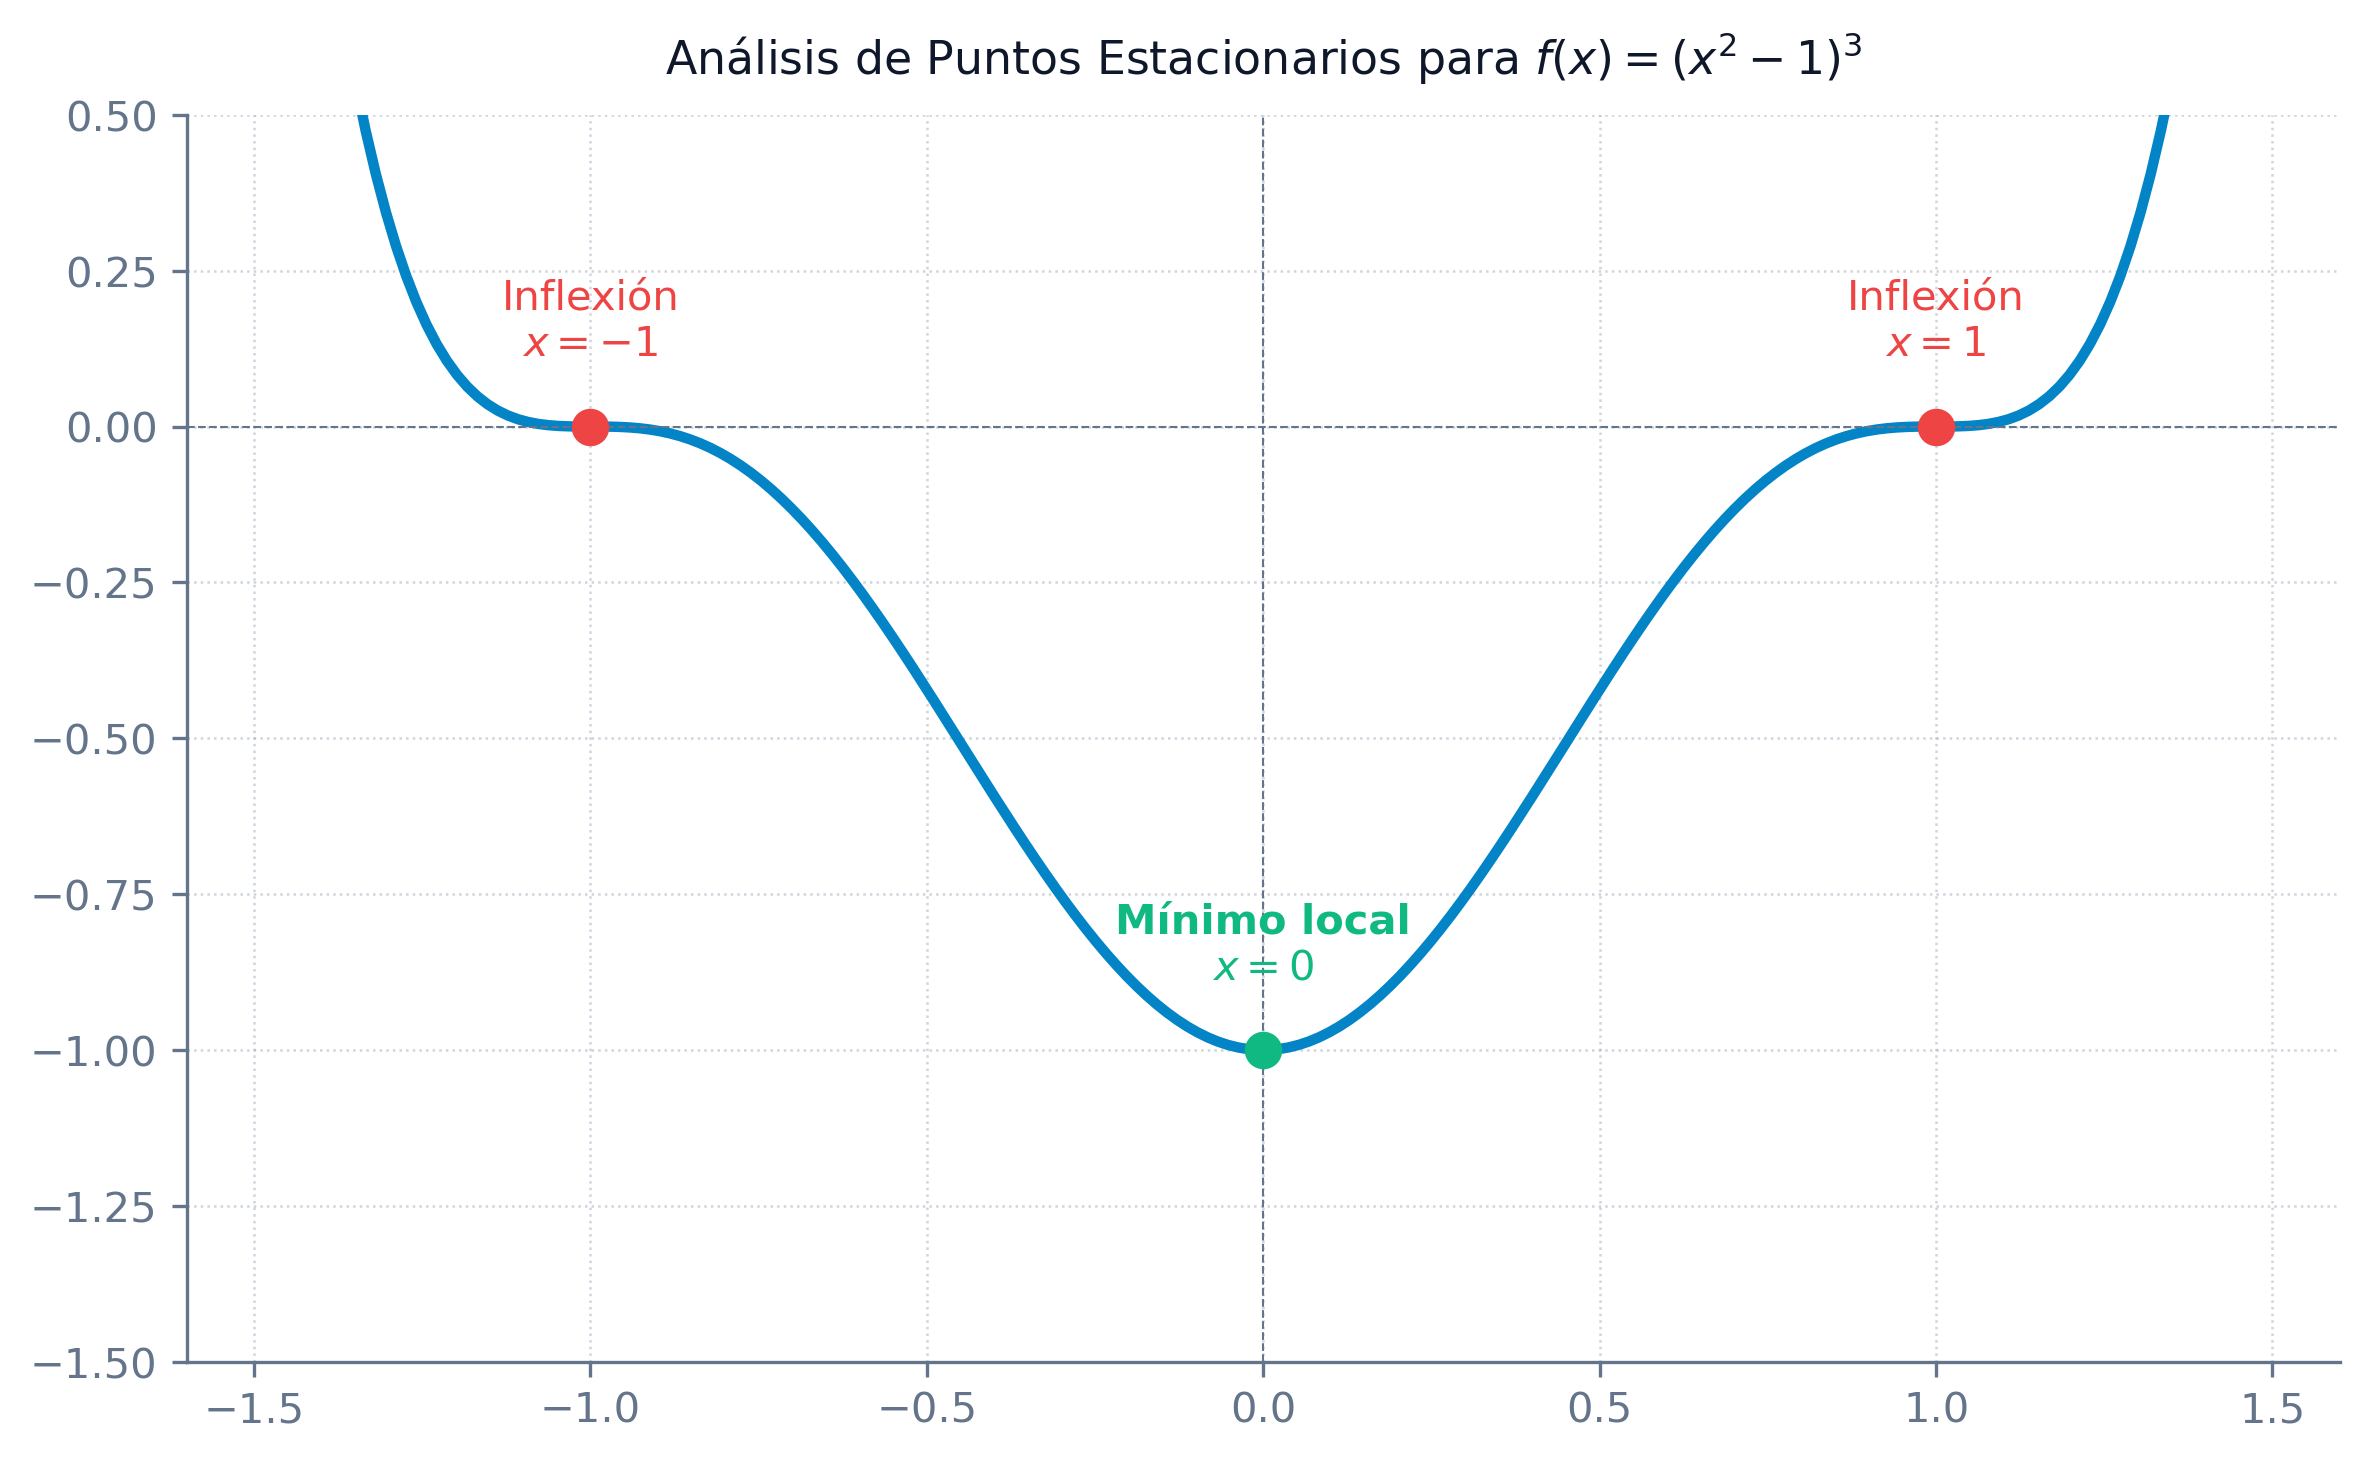
\includegraphics[width=0.7\linewidth,height=\textheight,keepaspectratio]{images/opt_sin_rest_inflexion.png}

}

\caption{\label{fig-opt-sin-rest-inflexion}Análisis de puntos
estacionarios e inflexiones en la función \(f(x)=(x^2-1)^3\)}

\end{figure}%

\end{tcolorbox}

\section{Optimización con
restricciones}\label{optimizaciuxf3n-con-restricciones}

En la práctica, la optimización matemática adquiere su verdadera
complejidad cuando introducimos limitaciones sobre las variables de
decisión. Para analizar formalmente estos problemas, inicialmente
consideraremos el marco general en el que la región factible
\(\mathcal{S} \subseteq \mathbb{R}^n\) es un conjunto genérico:
\[ \min \{ f(x) \mid x \in \mathcal{S} \} \] Posteriormente, nos
centraremos en problemas donde la región factible está definida
explícitamente mediante una serie de desigualdades analíticas:
\[ \min \{ f(x) \mid x \in \mathcal{X}, \ g_i(x) \le 0, \ i = 1, \dots, m \} \]
donde el dominio de partida \(\mathcal{X}\) es un abierto no vacío de
\(\mathbb{R}^n\) y tanto la función objetivo \(f\) como las
restricciones \(g_i\) son funciones diferenciables.

Para caracterizar si un punto frontera \(\bar{x} \in \mathcal{S}\) puede
ser un mínimo local, debemos analizar si es posible realizar un
movimiento infinitesimal a partir de él que cumpla dos condiciones:
permanecer dentro de la región factible \(\mathcal{S}\) y,
simultáneamente, disminuir el valor de la función objetivo \(f(x)\). En
términos geométricos, esto se estudia a través del concepto de
\textbf{conos de direcciones}:

\textbf{Cono de Direcciones Factibles (\(\mathcal{F}(\bar{x})\))} El
conjunto de direcciones a lo largo de las cuales un paso infinitesimal
no abandona la región factible \(\mathcal{S}\):
\[ \mathcal{F}(\bar{x}) = \{ d \in \mathbb{R}^n \mid d \neq 0, \ \exists \delta_d > 0 \text{ tal que } \bar{x} + \lambda d \in \mathcal{S}, \ \forall \lambda \in (0, \delta_d) \} \]

\textbf{Cono de Direcciones de Mejora/Descenso
(\(\mathcal{D}(\bar{x})\))} El conjunto de direcciones a lo largo de las
cuales el valor de la función objetivo disminuye localmente:
\[ \mathcal{D}(\bar{x}) = \{ d \in \mathbb{R}^n \mid d \neq 0, \ \exists \delta_d > 0 \text{ tal que } f(\bar{x} + \lambda d) < f(\bar{x}), \ \forall \lambda \in (0, \delta_d) \} \]

La condición básica de optimalidad geométrica establece que, si
\(\bar{x}\) es un mínimo local, es imposible encontrar una dirección que
nos permita adentrarnos en la región factible y, al mismo tiempo,
mejorar la función. En términos de conjuntos, esto significa que ambos
conos son disjuntos:
\[ \bar{x} \text{ es mínimo local} \implies \mathcal{F}(\bar{x}) \cap \mathcal{D}(\bar{x}) = \emptyset \]

Como se ilustra en la Figura~\ref{fig-cono-direcciones}, en un punto
mínimo local \(\bar{x}\) situado en la frontera de la región factible
\(\mathcal{S}\), el cono de direcciones factibles
\(\mathcal{F}(\bar{x})\) (que apunta hacia el interior de
\(\mathcal{S}\)) y el cono de direcciones de descenso analítico
\(\mathcal{D}_0(\bar{x})\) (que apunta en la dirección opuesta al
gradiente de la función objetivo \(\nabla f(\bar{x})\)) están
completamente separados, compartiendo únicamente el origen \(\bar{x}\).
Esto representa geométricamente que ninguna dirección admisible puede
disminuir localmente el valor del objetivo.

\begin{figure}

\centering{

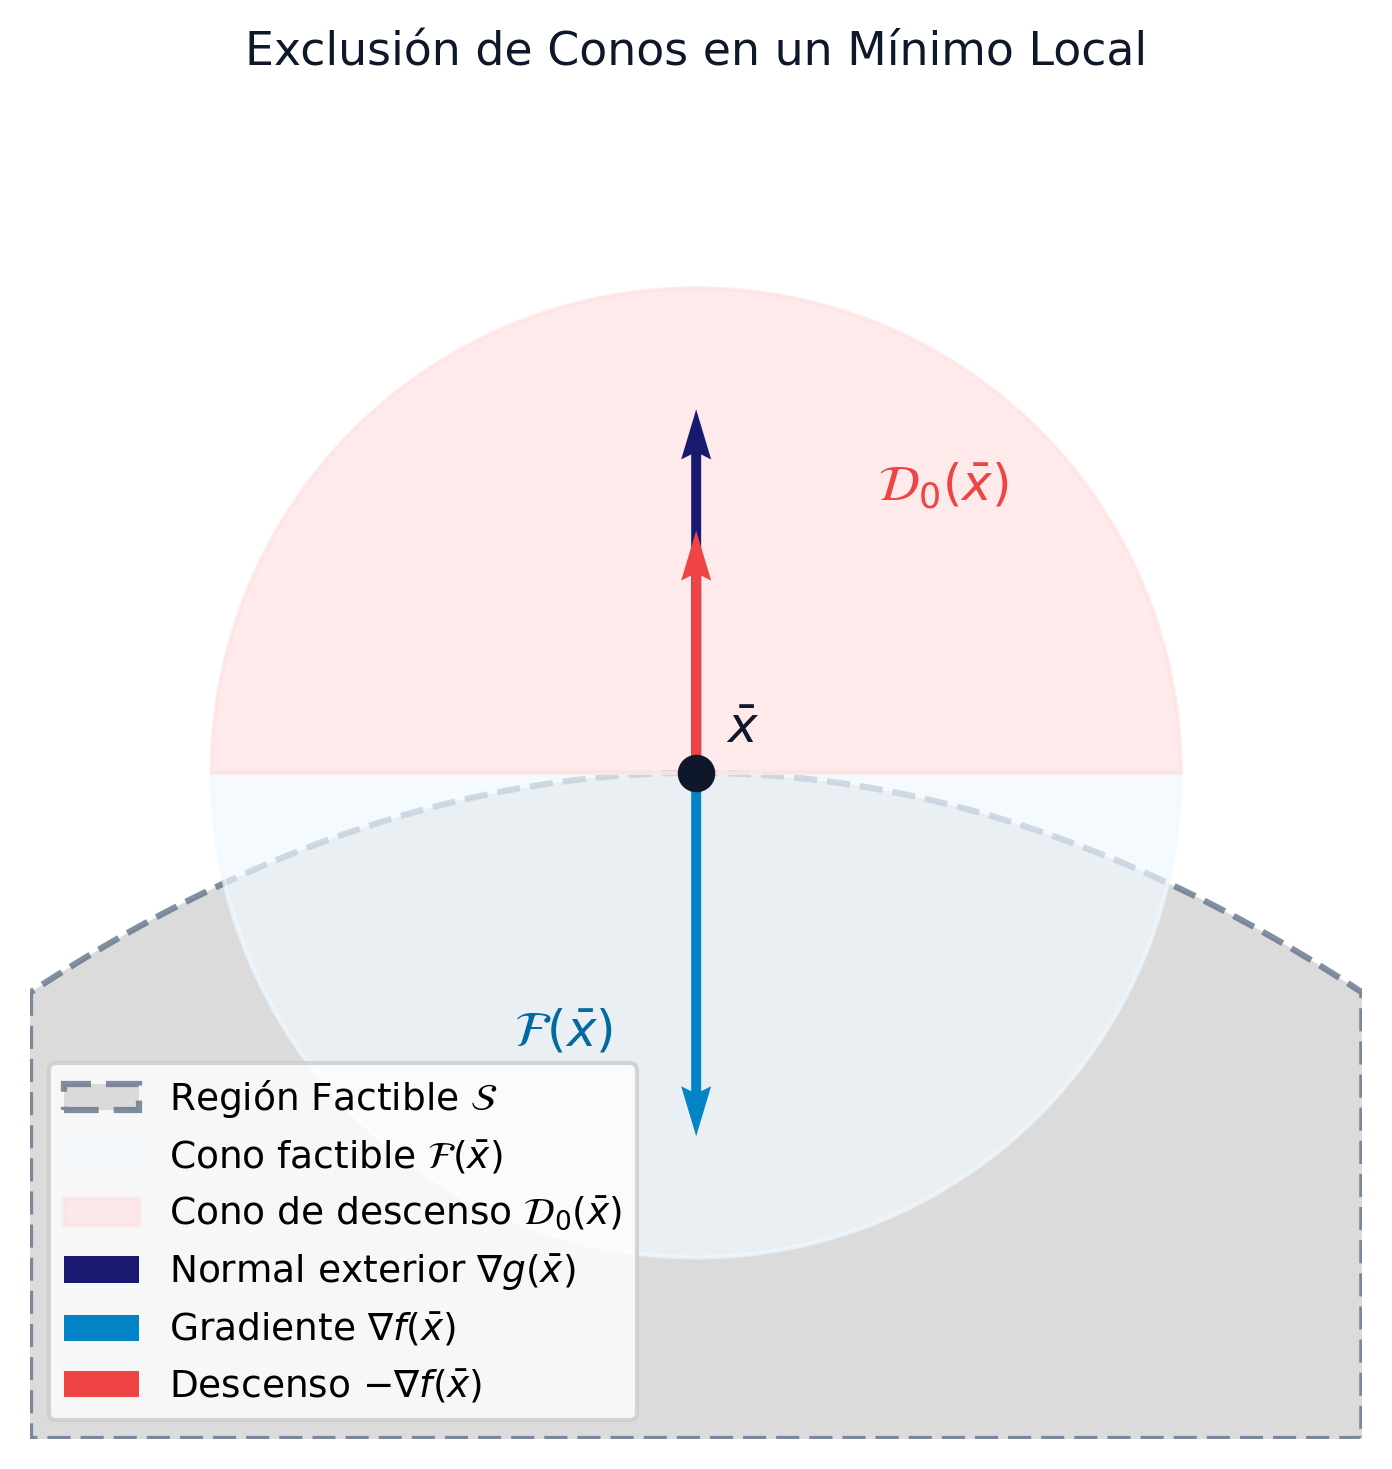
\includegraphics[width=0.6\linewidth,height=\textheight,keepaspectratio]{images/cono_direcciones.png}

}

\caption{\label{fig-cono-direcciones}Exclusión geométrica de los conos
factible y de descenso en un mínimo local}

\end{figure}%

Sin embargo, comprobar la exclusión geométrica directa es muy complejo
porque no siempre es fácil determinar analíticamente el cono de
direcciones de descenso real \(\mathcal{D}(\bar{x})\). Si la función
\(f\) es diferenciable en \(\bar{x}\), podemos simplificar la
caracterización del cono de descenso aproximándolo mediante un
semiespacio abierto definido por el gradiente. Definimos el cono de
direcciones de descenso analítico como el conjunto de direcciones que
forman un ángulo obtuso con el gradiente de la función en dicho punto:
\[ \mathcal{D}_0(\bar{x}) = \{ d \in \mathbb{R}^n \mid \nabla f(\bar{x})^T d < 0 \} \]
Este cono analítico siempre es un subconjunto del cono de descenso real
(\(\mathcal{D}_0(\bar{x}) \subseteq \mathcal{D}(\bar{x})\)). Esta
relación nos permite formular el primer criterio necesario de
optimalidad bajo restricciones diferenciables:

\begin{tcolorbox}[enhanced jigsaw, toprule=.15mm, opacitybacktitle=0.6, coltitle=black, colbacktitle=quarto-callout-important-color!10!white, title=\textcolor{quarto-callout-important-color}{\faExclamation}\hspace{0.5em}{Teorema: Exclusión de direcciones de descenso y factibilidad}, arc=.35mm, rightrule=.15mm, toptitle=1mm, breakable, bottomtitle=1mm, titlerule=0mm, colback=white, opacityback=0, leftrule=.75mm, colframe=quarto-callout-important-color-frame, left=2mm, bottomrule=.15mm]

Si \(\bar{x} \in \mathcal{S}\) es un mínimo local de una función
diferenciable \(f\), entonces el cono de direcciones factibles y el
semiespacio de descenso analítico son disjuntos:
\[ \mathcal{D}_0(\bar{x}) \cap \mathcal{F}(\bar{x}) = \emptyset \]

\emph{Demostración}: Supóngase por contradicción que existe un vector
\(d \in \mathcal{D}_0(\bar{x}) \cap \mathcal{F}(\bar{x})\). 1. Como
\(d \in \mathcal{D}_0(\bar{x})\), se cumple que
\(\nabla f(\bar{x})^T d < 0\). Por el Teorema de Dirección de Descenso,
existe un paso \(\delta_1 > 0\) tal que
\(f(\bar{x} + \lambda d) < f(\bar{x})\) para todo
\(\lambda \in (0, \delta_1)\). 2. Como \(d \in \mathcal{F}(\bar{x})\),
por definición de cono factible, existe un paso \(\delta_2 > 0\) tal que
\(\bar{x} + \lambda d \in \mathcal{S}\) para todo
\(\lambda \in (0, \delta_2)\). Tomando el paso mínimo
\(\delta = \min \{\delta_1, \delta_2\} > 0\), se deduce que para todo
\(\lambda \in (0, \delta)\) el punto \(\bar{x} + \lambda d\) es factible
y además \(f(\bar{x} + \lambda d) < f(\bar{x})\), lo que contradice
directamente que \(\bar{x}\) sea un mínimo local de \(f\) en la región
factible. \(\blacksquare\)

\end{tcolorbox}

La condición de exclusión anterior
(\(\mathcal{D}_0(\bar{x}) \cap \mathcal{F}(\bar{x}) = \emptyset\)) es de
carácter necesario. La implicación inversa (suficiencia) no se cumple en
general debido a que si el gradiente se anula
(\(\nabla f(\bar{x}) = 0\)), el cono analítico se vacía
(\(\mathcal{D}_0(\bar{x}) = \emptyset\)), pero el punto podría ser un
máximo o un punto de silla y no un mínimo. Sin embargo, si la función
objetivo es pseudo-convexa y la región factible cumple condiciones
locales de regularidad, esta condición necesaria se convierte también en
suficiente para garantizar la optimalidad, tal como establece el
siguiente teorema:

\begin{tcolorbox}[enhanced jigsaw, toprule=.15mm, opacitybacktitle=0.6, coltitle=black, colbacktitle=quarto-callout-important-color!10!white, title=\textcolor{quarto-callout-important-color}{\faExclamation}\hspace{0.5em}{Teorema: Suficiencia geométrica bajo pseudo-convexidad}, arc=.35mm, rightrule=.15mm, toptitle=1mm, breakable, bottomtitle=1mm, titlerule=0mm, colback=white, opacityback=0, leftrule=.75mm, colframe=quarto-callout-important-color-frame, left=2mm, bottomrule=.15mm]

Sea el problema de optimización \(\min\{f(x) \mid x \in \mathcal{S}\}\),
con \(f\) diferenciable y pseudo-convexa en \(\bar{x} \in \mathcal{S}\).
Si \(\mathcal{D}_0(\bar{x}) \cap \mathcal{F}(\bar{x}) = \emptyset\) y
existe un entorno \(N_\epsilon(\bar{x})\) de radio \(\epsilon > 0\) tal
que \(d = (x - \bar{x}) \in \mathcal{F}(\bar{x})\) para cualquier
\(x \in \mathcal{S} \cap N_\epsilon(\bar{x})\), entonces \(\bar{x}\) es
un mínimo local de \(f\).

\emph{Demostración}: Supóngase por contradicción que \(\bar{x}\) no es
mínimo local. Entonces existe un punto
\(\hat{x} \in \mathcal{S} \cap N_\epsilon(\bar{x})\) tal que
\(f(\hat{x}) < f(\bar{x})\). Por la hipótesis del entorno, el vector
\(d = \hat{x} - \bar{x}\) pertenece al cono factible
\(\mathcal{F}(\bar{x})\). Por ser \(f\) pseudo-convexa en \(\bar{x}\),
se cumple que:
\[ f(\hat{x}) < f(\bar{x}) \implies \nabla f(\bar{x})^T d < 0 \implies d \in \mathcal{D}_0(\bar{x}) \]
Por tanto, \(d \in \mathcal{D}_0(\bar{x}) \cap \mathcal{F}(\bar{x})\),
lo cual contradice que dicha intersección sea vacía. \(\blacksquare\)

\end{tcolorbox}

Aunque la caracterización
\(\mathcal{D}_0(\bar{x}) \cap \mathcal{F}(\bar{x}) = \emptyset\)
simplifica el cono de descenso gracias al uso del gradiente
\(\nabla f(\bar{x})\), seguimos teniendo el inconveniente principal de
no disponer de una representación algebraica manejable del cono de
direcciones factibles \(\mathcal{F}(\bar{x})\).

\begin{tcolorbox}[enhanced jigsaw, toprule=.15mm, opacitybacktitle=0.6, coltitle=black, colbacktitle=quarto-callout-warning-color!10!white, title=\textcolor{quarto-callout-warning-color}{\faExclamationTriangle}\hspace{0.5em}{Limitación del cono de direcciones factibles}, arc=.35mm, rightrule=.15mm, toptitle=1mm, breakable, bottomtitle=1mm, titlerule=0mm, colback=white, opacityback=0, leftrule=.75mm, colframe=quarto-callout-warning-color-frame, left=2mm, bottomrule=.15mm]

El cono de direcciones factibles \(\mathcal{F}(\bar{x})\) se define de
forma puramente geométrica y depende del comportamiento infinitesimal de
la frontera de la región factible \(\mathcal{S}\). En la práctica,
determinar analíticamente si una dirección \(d\) pertenece a
\(\mathcal{F}(\bar{x})\) requiere analizar la existencia de un paso
\(\delta > 0\) tal que \(\bar{x} + \lambda d \in \mathcal{S}\) para todo
\(\lambda \in (0, \delta)\). Esto resulta extremadamente difícil e
ineficiente cuando las restricciones son no lineales.

Para resolver esta limitación, si la región factible está definida por
restricciones de desigualdad diferenciables, aproximamos localmente el
cono factible \(\mathcal{F}(\bar{x})\) mediante el cono de restricciones
activas \(\mathcal{G}_0(\bar{x})\), el cual se define de forma puramente
algebraica a partir de los gradientes de las restricciones activas.

\end{tcolorbox}

\section{Restricciones de desigualdad y cono de restricciones
activas}\label{restricciones-de-desigualdad-y-cono-de-restricciones-activas}

A partir de este momento, nos centraremos en el caso en el que la región
factible \(\mathcal{S}\) está definida explícitamente mediante una serie
de desigualdades analíticas:
\[ \mathcal{S} = \{ x \in \mathcal{X} \mid g_i(x) \le 0, \ i = 1, \dots, m \} \]
donde \(\mathcal{X} \subseteq \mathbb{R}^n\) es un conjunto abierto no
vacío. En este marco, las direcciones a lo largo de las cuales nos
podemos mover localmente desde un punto \(\bar{x} \in \mathcal{S}\)
dependen de qué restricciones se satisfacen con igualdad en dicho punto,
ya que las restricciones estrictamente negativas (\(g_i(\bar{x}) < 0\))
no limitan el movimiento infinitesimal en un entorno suficientemente
pequeño.

\textbf{Restricciones Activas (\(\mathcal{I}\))} Dado un punto factible
\(\bar{x} \in \mathcal{S}\), el conjunto de índices de las restricciones
activas en \(\bar{x}\) se define como:
\[ \mathcal{I} = \{ i \in \{1, \dots, m\} \mid g_i(\bar{x}) = 0 \} \]
Por conveniencia, si no da lugar a confusión, denotaremos este conjunto
simplemente como \(\mathcal{I}\).

Para las restricciones activas, si \(g_i\) es diferenciable, el vector
gradiente \(\nabla g_i(\bar{x})\) señala la dirección de máximo
crecimiento local de la restricción. Puesto que las restricciones son de
tipo ``menor o igual que'' (\(g_i(x) \le 0\)), el gradiente
\(\nabla g_i(\bar{x})\) apunta hacia el exterior de la región factible.
Si una dirección \(d\) forma un ángulo obtuso con este gradiente
(\(\nabla g_i(\bar{x})^T d < 0\)), nos moveremos localmente hacia el
interior factible de dicha restricción.

\begin{tcolorbox}[enhanced jigsaw, toprule=.15mm, opacitybacktitle=0.6, coltitle=black, colbacktitle=quarto-callout-tip-color!10!white, title=\textcolor{quarto-callout-tip-color}{\faLightbulb}\hspace{0.5em}{Ejemplo: Identificación de restricciones activas, gradientes y
direcciones factibles}, arc=.35mm, rightrule=.15mm, toptitle=1mm, breakable, bottomtitle=1mm, titlerule=0mm, colback=white, opacityback=0, leftrule=.75mm, colframe=quarto-callout-tip-color-frame, left=2mm, bottomrule=.15mm]

Consideremos el siguiente problema bidimensional: \[
\begin{aligned}
\min \quad & f(x_1, x_2) = (x_1 - 3)^2 + (x_2 - 2)^2 \\
\text{s.a.} \quad & g_1(x_1, x_2) = x_1^2 + x_2^2 - 5 \le 0 \\
& g_2(x_1, x_2) = -x_1 \le 0 \\
& g_3(x_1, x_2) = -x_2 \le 0 \\
& g_4(x_1, x_2) = x_1 + x_2 - 3 \le 0
\end{aligned}
\] En la Figura~\ref{fig-active-constraints-intro} se representa la
región factible \(\mathcal{S}\) y las fronteras de las restricciones.
Dependiendo de la ubicación del punto factible de interés, el conjunto
de restricciones activas \(\mathcal{I}\) varía considerablemente:

\begin{itemize}
\tightlist
\item
  \textbf{En el punto \((1,1)\)}: El punto es estrictamente interior,
  por lo que ninguna restricción se cumple con igualdad y
  \(\mathcal{I} = \emptyset\).
\item
  \textbf{En el punto \((0,0)\)}: El punto está en el origen, lo que
  activa las fronteras del primer cuadrante, resultando
  \(\mathcal{I} = \{2, 3\}\).
\item
  \textbf{En el punto \((2,1)\)}: El punto está sobre la intersección de
  la circunferencia y la recta inclinada, activando simultáneamente
  ambas fronteras, resultando \(\mathcal{I} = \{1, 4\}\).
\item
  \textbf{En el punto \((0,1)\)}: El punto está en el eje vertical, lo
  que activa únicamente la restricción de no negatividad de \(x_1\),
  resultando \(\mathcal{I} = \{2\}\).
\end{itemize}

\begin{figure}[H]

\centering{

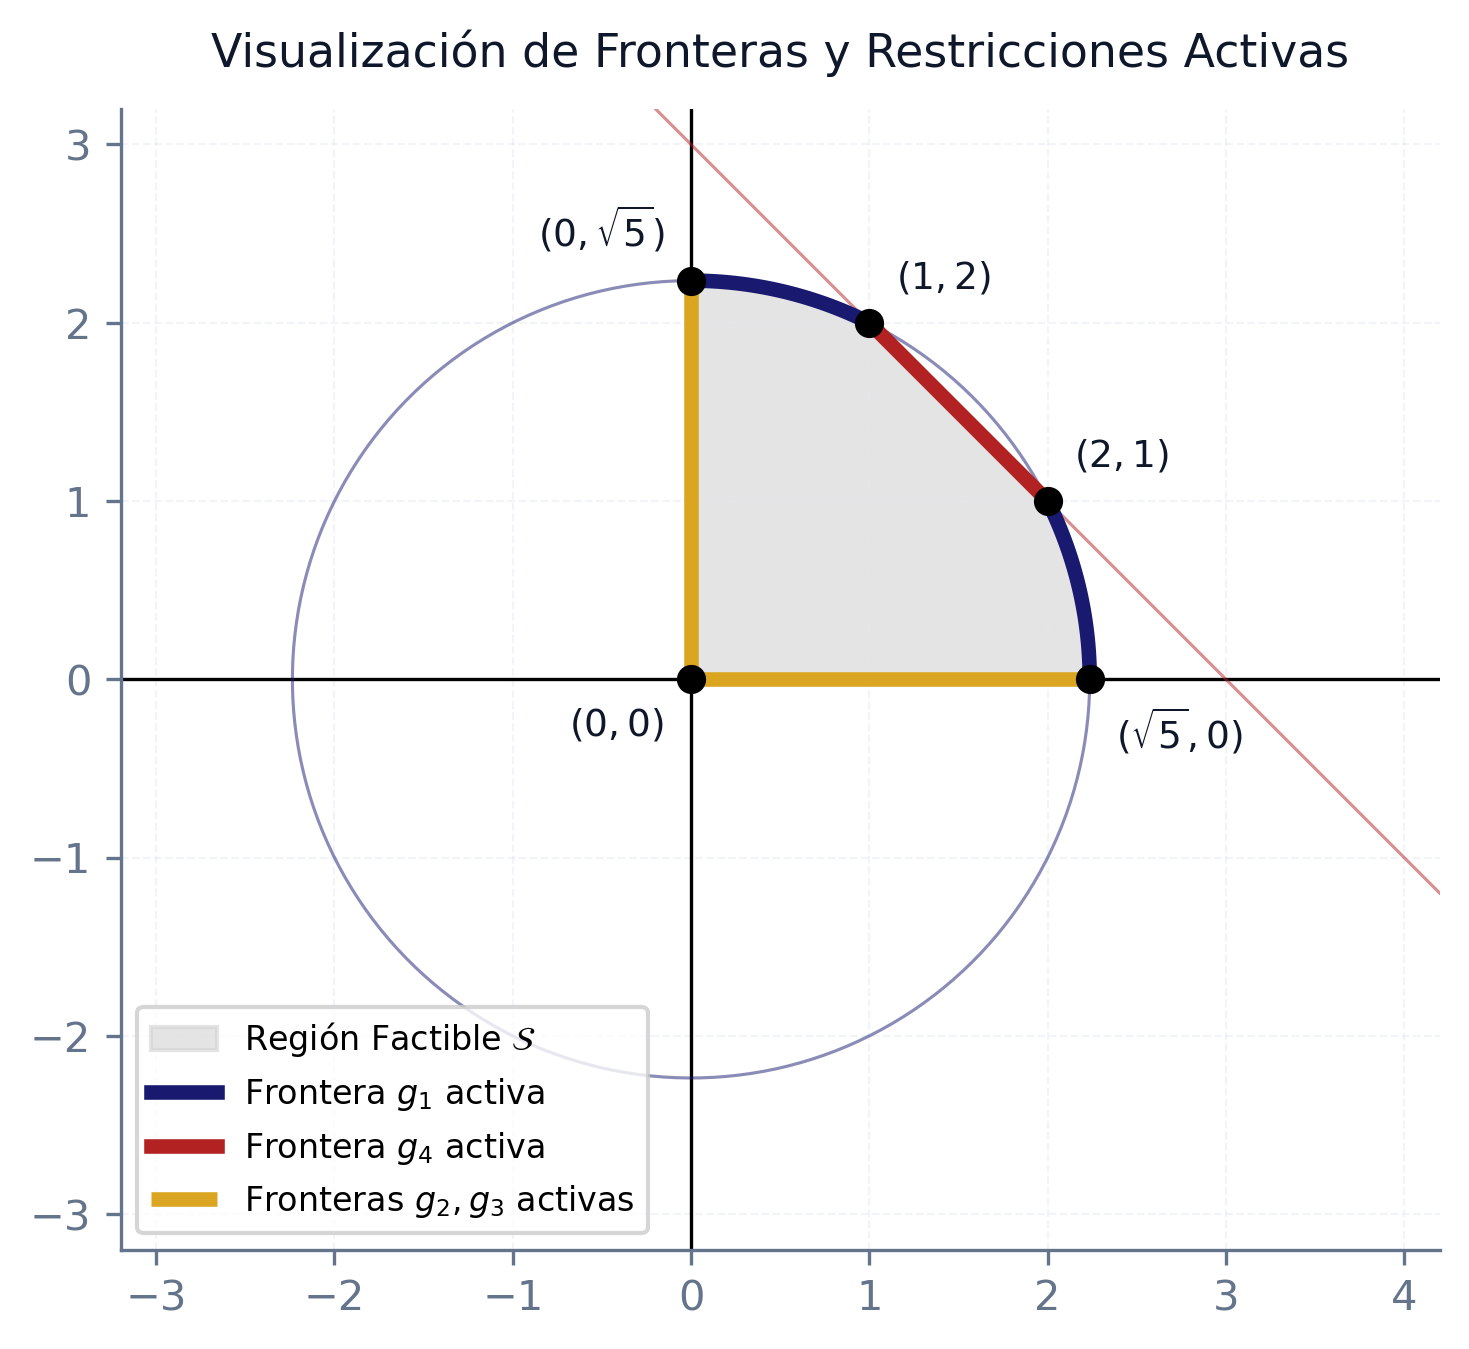
\includegraphics[width=0.6\linewidth,height=\textheight,keepaspectratio]{images/active_constraints_intro.png}

}

\caption{\label{fig-active-constraints-intro}Visualización de la región
factible y del conjunto de restricciones activas para distintos puntos
candidatos}

\end{figure}%

Si evaluamos los gradientes de las restricciones activas en los puntos
de la frontera, observamos que, debido a que el problema está formulado
con desigualdades de tipo menor o igual (\(g_i(x) \le 0\)), dichos
vectores apuntan siempre hacia el exterior del conjunto factible
\(\mathcal{S}\).

Por ejemplo, en el punto \((1,2)\), la restricción circular \(g_1\) y la
restricción lineal \(g_4\) son activas. Sus respectivos gradientes en
dicho punto son \(\nabla g_1(1,2) = (2,4)^T\) y
\(\nabla g_4(1,2) = (1,1)^T\). Como se ilustra en la
Figura~\ref{fig-active-constraints-gradients}, ambos vectores señalan
hacia fuera de la región factible.

\begin{figure}[H]

\centering{

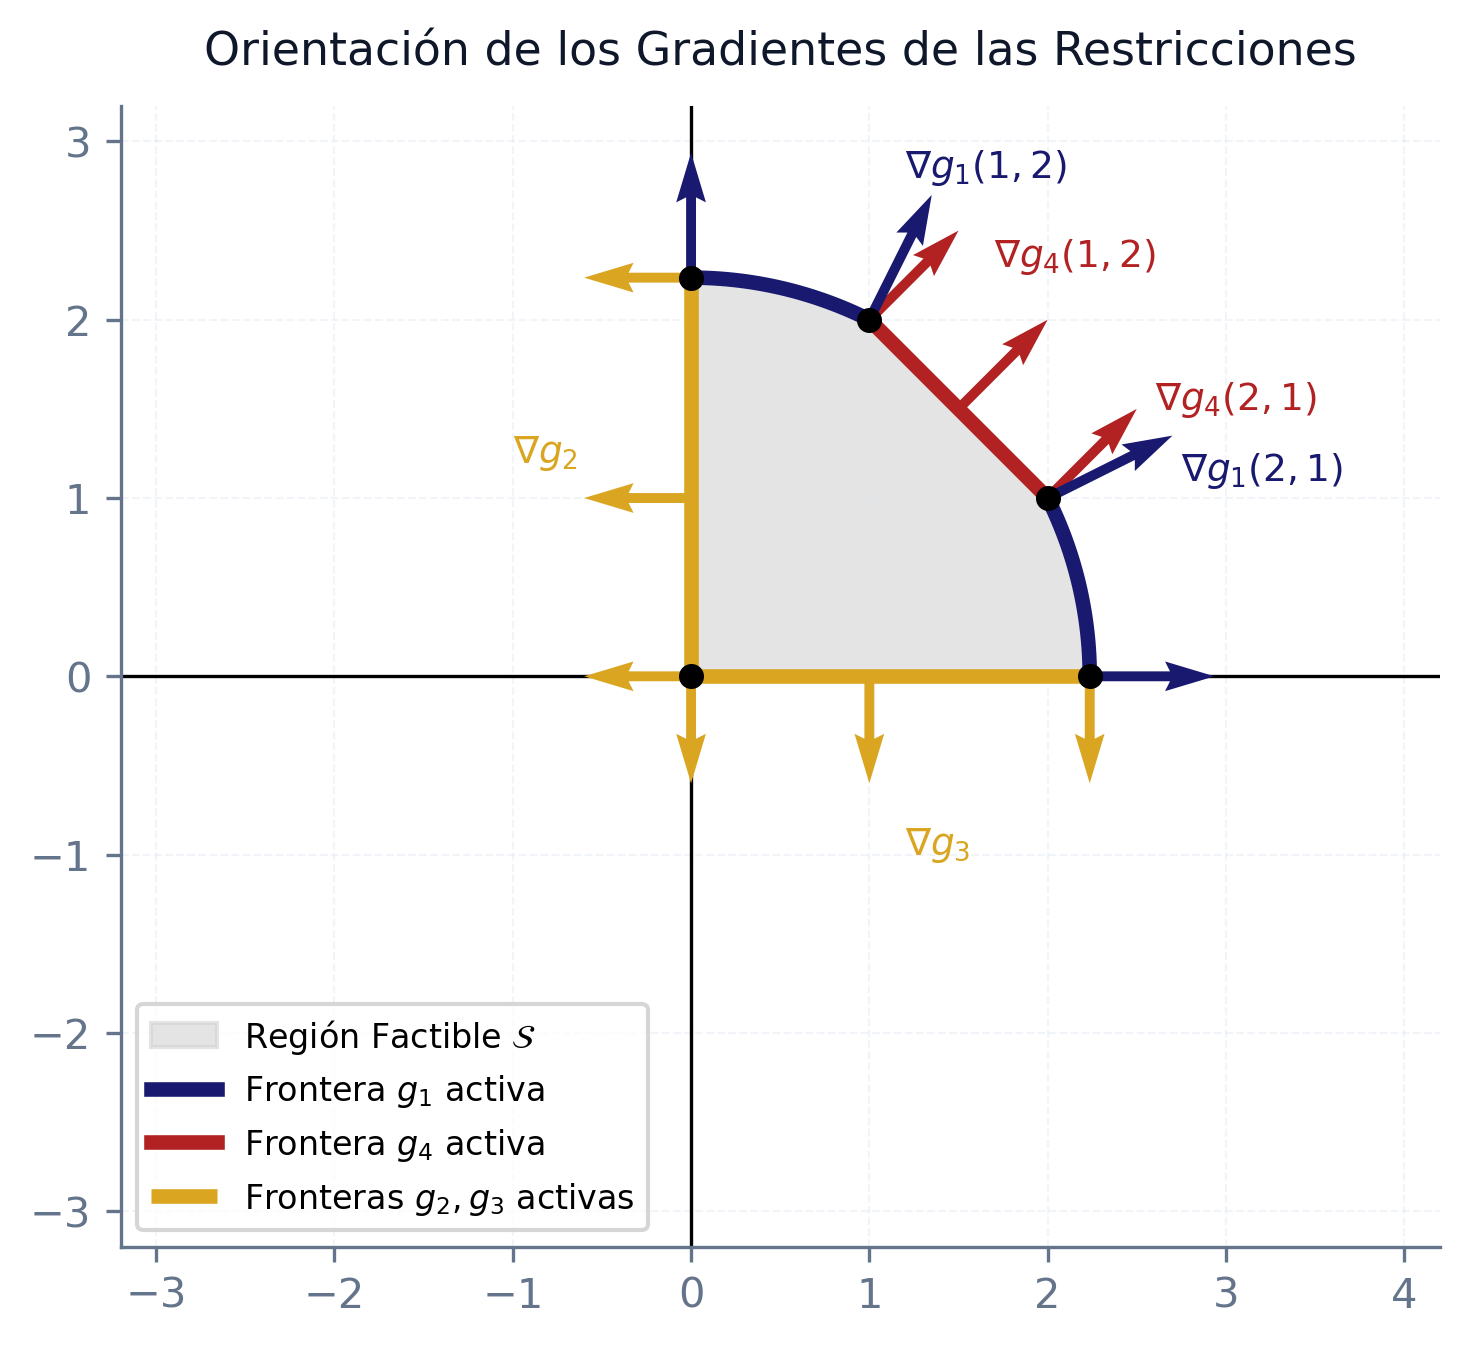
\includegraphics[width=0.6\linewidth,height=\textheight,keepaspectratio]{images/active_constraints_gradients.png}

}

\caption{\label{fig-active-constraints-gradients}Orientación de los
gradientes de las restricciones en la frontera de la región factible}

\end{figure}%

Además, consideremos qué ocurre cuando una dirección \(d\) es ortogonal
al gradiente de una restricción activa lineal, es decir,
\(\nabla g_i(\bar{x})^T d = 0\). Como se observa en la
Figura~\ref{fig-active-constraints-orthogonality}:

\begin{itemize}
\tightlist
\item
  \textbf{En el punto \((0,1)\)} de la frontera vertical (eje \(x_2\)),
  la restricción \(g_2(x) = -x_1 \le 0\) está activa, con gradiente
  \(\nabla g_2(0,1) = (-1,0)^T\). La dirección \(d = (0,1)^T\) (que
  apunta verticalmente hacia arriba) es ortogonal a dicho gradiente
  (\(\nabla g_2^T d = 0\)). Sin embargo, moverse en la dirección \(d\)
  mantiene al punto sobre la frontera, por lo que \(d\) es una dirección
  factible.
\item
  \textbf{En el punto \((1,2)\)} de la frontera lineal oblicua, la
  restricción \(g_4(x) = x_1+x_2-3 \le 0\) está activa, con gradiente
  \(\nabla g_4(1,2) = (1,1)^T\). La dirección \(d = (1,-1)^T\) (que
  apunta hacia abajo y a la derecha a lo largo de la recta) es ortogonal
  al gradiente (\(\nabla g_4^T d = 0\)). No obstante, al ser la
  restricción lineal, la dirección \(d\) es completamente factible.
\end{itemize}

\begin{figure}[H]

\centering{

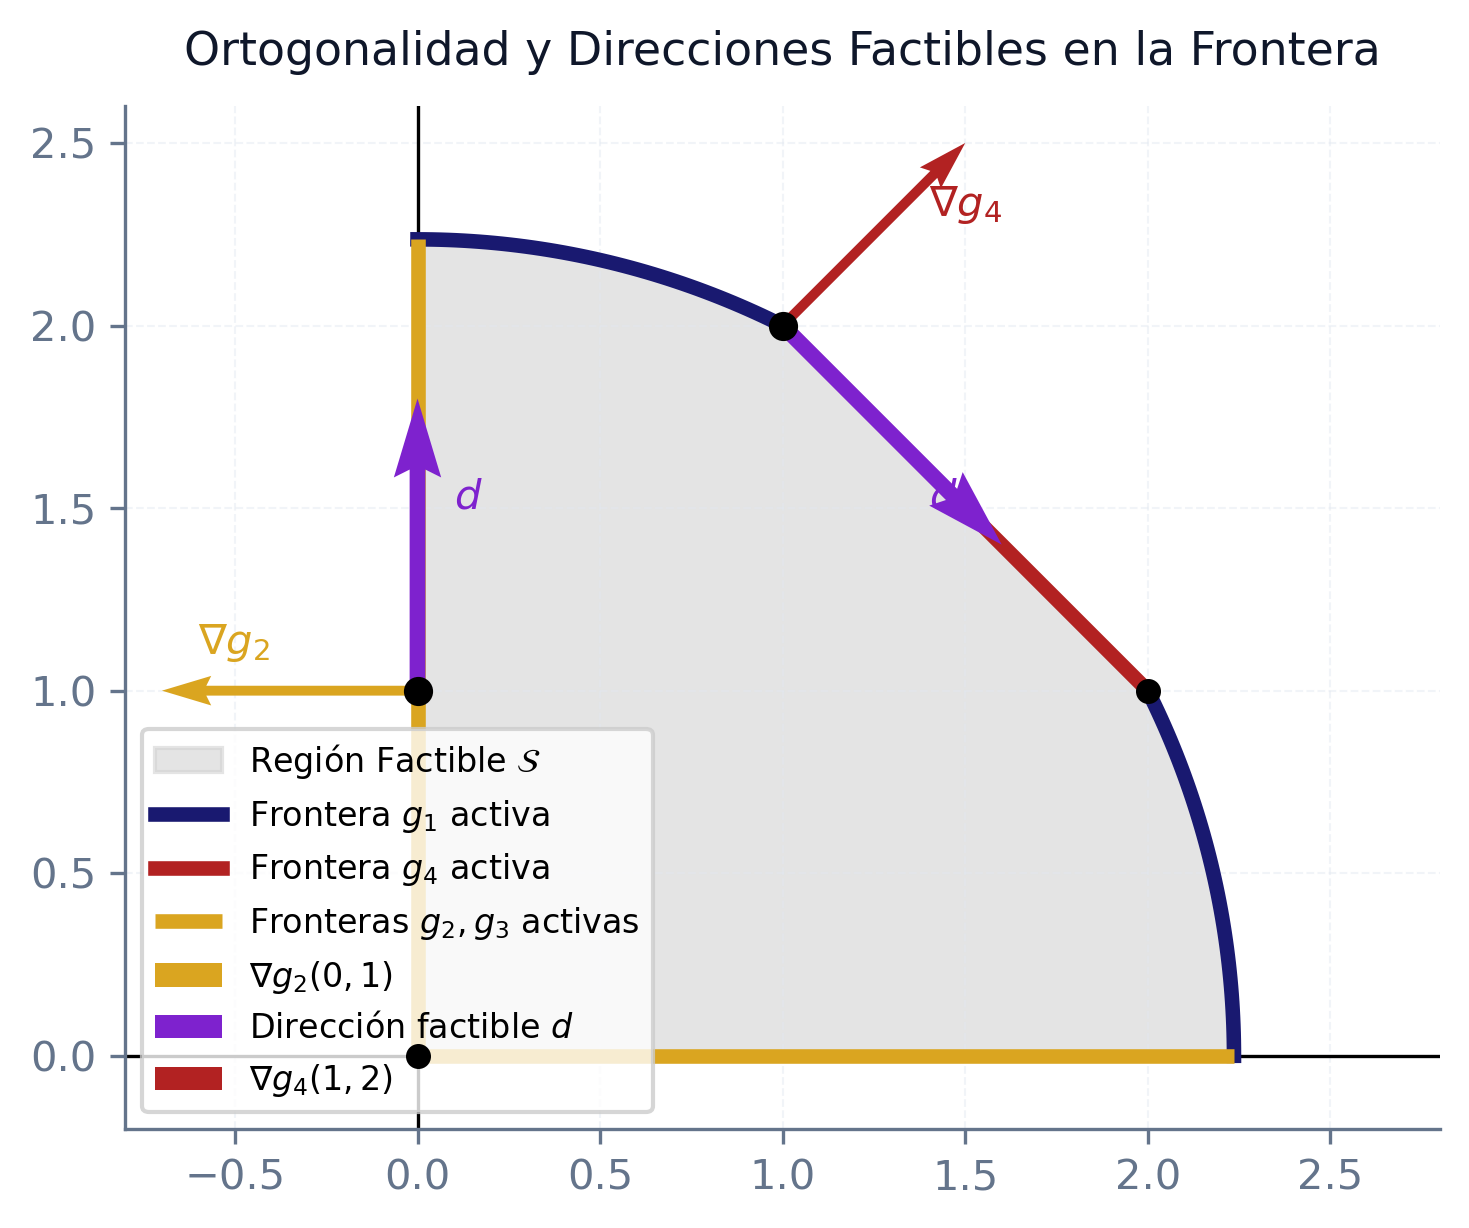
\includegraphics[width=0.6\linewidth,height=\textheight,keepaspectratio]{images/active_constraints_orthogonality.png}

}

\caption{\label{fig-active-constraints-orthogonality}Direcciones
factibles ortogonales a los gradientes en fronteras lineales}

\end{figure}%

\end{tcolorbox}

Esto nos permite definir el cono de direcciones factibles analíticas o
algebraicas asociado a las restricciones activas como:
\[ \mathcal{G}_0(\bar{x}) = \{ d \in \mathbb{R}^n \mid \nabla g_i(\bar{x})^T d < 0, \ \forall i \in \mathcal{I} \} \]

La relación entre este cono algebraico y el cono factible geométrico
\(\mathcal{F}(\bar{x})\) es estrecha, pero presenta matices importantes.
Si una dirección \(d\) pertenece a \(\mathcal{G}_0(\bar{x})\), es
factible respecto a todas las restricciones activas. No obstante,
\(\mathcal{G}_0(\bar{x})\) es, en general, un subconjunto estricto del
cono factible geométrico
(\(\mathcal{G}_0(\bar{x}) \subseteq \mathcal{F}(\bar{x})\)). La igualdad
no siempre se cumple: por ejemplo, si una restricción \(g_i\) es lineal
y el vector \(d\) es ortogonal a su gradiente
(\(\nabla g_i(\bar{x})^T d = 0\)), la dirección \(d\) puede seguir
siendo factible (moviéndose por la frontera), pero no pertenecerá al
cono abierto \(\mathcal{G}_0(\bar{x})\).

A partir de esta inclusión
\(\mathcal{G}_0(\bar{x}) \subseteq \mathcal{F}(\bar{x})\), podemos
establecer una condición necesaria de optimalidad local más débil y de
más fácil verificación algebraica que la exclusión geométrica directa:

\begin{tcolorbox}[enhanced jigsaw, toprule=.15mm, opacitybacktitle=0.6, coltitle=black, colbacktitle=quarto-callout-important-color!10!white, title=\textcolor{quarto-callout-important-color}{\faExclamation}\hspace{0.5em}{Teorema: Intersección vacía con el cono de restricciones activas}, arc=.35mm, rightrule=.15mm, toptitle=1mm, breakable, bottomtitle=1mm, titlerule=0mm, colback=white, opacityback=0, leftrule=.75mm, colframe=quarto-callout-important-color-frame, left=2mm, bottomrule=.15mm]

Sea el problema de optimización bajo restricciones de desigualdad,
\(\bar{x}\) una solución factible e \(\mathcal{I}\) el conjunto de
restricciones activas en \(\bar{x}\). Si se verifican las siguientes
propiedades:

\begin{enumerate}
\def\labelenumi{\arabic{enumi}.}
\tightlist
\item
  \(f\) y las restricciones activas \(g_i\) (\(i \in \mathcal{I}\)) son
  diferenciables en \(\bar{x}\),
\item
  Las restricciones inactivas \(g_j\) (\(j \notin \mathcal{I}\)) son
  continuas en \(\bar{x}\),
\item
  \(\bar{x}\) es un mínimo local del problema,
\end{enumerate}

entonces el cono de descenso analítico y el cono de restricciones
activas son disjuntos:
\[ \mathcal{D}_0(\bar{x}) \cap \mathcal{G}_0(\bar{x}) = \emptyset \]

\emph{Demostración}: Sea \(d \in \mathcal{G}_0(\bar{x})\). Por
definición, se cumple que \(\nabla g_i(\bar{x})^T d < 0\) para todo
\(i \in \mathcal{I}\). Como las funciones \(g_i\)
(\(i \in \mathcal{I}\)) son diferenciables en \(\bar{x}\), aplicando el
Teorema de Dirección de Descenso, existe un paso \(\delta_1 > 0\) tal
que:
\[ g_i(\bar{x} + \lambda d) < g_i(\bar{x}) = 0, \quad \forall \lambda \in (0, \delta_1), \ \forall i \in \mathcal{I} \]
Para las restricciones inactivas (\(j \notin \mathcal{I}\)), dado que
\(g_j(\bar{x}) < 0\) y por la continuidad de \(g_j\) en \(\bar{x}\),
existe un entorno \(\delta_2 > 0\) tal que:
\[ g_j(\bar{x} + \lambda d) < 0, \quad \forall \lambda \in (0, \delta_2), \ \forall j \notin \mathcal{I} \]
Asimismo, por ser \(\mathcal{X}\) un conjunto abierto y
\(\bar{x} \in \mathcal{X}\), existe un paso \(\delta_3 > 0\) tal que:
\[ \bar{x} + \lambda d \in \mathcal{X}, \quad \forall \lambda \in (0, \delta_3) \]
Tomando el paso mínimo común
\(\delta = \min \{\delta_1, \delta_2, \delta_3\} > 0\), concluimos que
para todo \(\lambda \in (0, \delta)\) el punto \(\bar{x} + \lambda d\)
pertenece a \(\mathcal{X}\) y satisface todas las restricciones de
desigualdad (\(g_i(\bar{x} + \lambda d) < 0\), \(\forall i\)). Por
tanto, \(\bar{x} + \lambda d \in \mathcal{S}\) para todo
\(\lambda \in (0, \delta)\), lo que por definición implica que la
dirección es factible (\(d \in \mathcal{F}(\bar{x})\)).

Hemos demostrado así que
\(\mathcal{G}_0(\bar{x}) \subseteq \mathcal{F}(\bar{x})\). Por ser
\(\bar{x}\) un mínimo local del problema, el Teorema de Exclusión de
Direcciones de Descenso y Factibilidad garantiza que
\(\mathcal{D}_0(\bar{x}) \cap \mathcal{F}(\bar{x}) = \emptyset\). Dado
que \(\mathcal{G}_0(\bar{x})\) es un subconjunto de
\(\mathcal{F}(\bar{x})\), se concluye inmediatamente que su intersección
con el cono de descenso también debe ser vacía:
\[ \mathcal{D}_0(\bar{x}) \cap \mathcal{G}_0(\bar{x}) = \emptyset \] lo
que completa la demostración. \(\blacksquare\)

\end{tcolorbox}

La condición necesaria
\(\mathcal{D}_0(\bar{x}) \cap \mathcal{G}_0(\bar{x}) = \emptyset\) es
más débil que la geométrica
\(\mathcal{D}_0(\bar{x}) \cap \mathcal{F}(\bar{x}) = \emptyset\) (al ser
\(\mathcal{G}_0\) un cono más restrictivo). Sin embargo, bajo hipótesis
de convexidad generalizada sobre las restricciones y el objetivo, esta
condición es también suficiente para garantizar que un punto es mínimo
local, como establece el siguiente resultado:

\begin{tcolorbox}[enhanced jigsaw, toprule=.15mm, opacitybacktitle=0.6, coltitle=black, colbacktitle=quarto-callout-important-color!10!white, title=\textcolor{quarto-callout-important-color}{\faExclamation}\hspace{0.5em}{Teorema: Suficiencia geométrica sin KKT}, arc=.35mm, rightrule=.15mm, toptitle=1mm, breakable, bottomtitle=1mm, titlerule=0mm, colback=white, opacityback=0, leftrule=.75mm, colframe=quarto-callout-important-color-frame, left=2mm, bottomrule=.15mm]

Sea el problema de optimización bajo restricciones de desigualdad, con
\(f\) y \(g_i\) diferenciables en el punto factible \(\bar{x}\). Si se
verifican las siguientes condiciones:

\begin{enumerate}
\def\labelenumi{\arabic{enumi}.}
\tightlist
\item
  \(f\) es pseudo-convexa en \(\bar{x}\),
\item
  Las restricciones activas \(g_i\) (\(i \in \mathcal{I}\)) son
  estrictamente pseudo-convexas en \(\bar{x}\),
\item
  \(\mathcal{D}_0(\bar{x}) \cap \mathcal{G}_0(\bar{x}) = \emptyset\),
\end{enumerate}

entonces \(\bar{x}\) es un mínimo local del problema.

\emph{Demostración}: Supongamos por contradicción que \(\bar{x}\) no es
un mínimo local. Entonces existe un punto factible \(x \in \mathcal{S}\)
tal que \(f(x) < f(\bar{x})\). Por la diferenciabilidad y
pseudo-convexidad de \(f\) en \(\bar{x}\), se cumple que:
\[ f(x) < f(\bar{x}) \implies \nabla f(\bar{x})^T (x - \bar{x}) < 0 \]
Definiendo la dirección \(d = x - \bar{x}\), esto implica directamente
que \(d \in \mathcal{D}_0(\bar{x})\).

Por otro lado, para cualquier restricción activa \(i \in \mathcal{I}\),
dado que \(x \in \mathcal{S}\), se tiene que \(g_i(x) \le 0\). Al ser la
restricción activa en el punto de comparación, \(g_i(\bar{x}) = 0\), lo
que implica que \(g_i(x) \le g_i(\bar{x})\). Dado que las restricciones
activas \(g_i\) son estrictamente pseudo-convexas en \(\bar{x}\), se
tiene por definición de estricta pseudo-convexidad:
\[ g_i(x) \le g_i(\bar{x}) \implies \nabla g_i(\bar{x})^T (x - \bar{x}) < 0 \]
Como esta relación se verifica para todos los índices activos
\(i \in \mathcal{I}\), se concluye que:
\[ \nabla g_i(\bar{x})^T d < 0, \quad \forall i \in \mathcal{I} \implies d \in \mathcal{G}_0(\bar{x}) \]
Por consiguiente,
\(d \in \mathcal{D}_0(\bar{x}) \cap \mathcal{G}_0(\bar{x})\), lo cual
contradice de forma directa la hipótesis de que la intersección
\(\mathcal{D}_0(\bar{x}) \cap \mathcal{G}_0(\bar{x})\) es vacía. Por
tanto, \(\bar{x}\) es un mínimo local. \(\blacksquare\)

\end{tcolorbox}

Este teorema de suficiencia establece que la ausencia de direcciones
factibles de descenso es garantía de optimalidad local bajo ciertas
condiciones de regularidad y convexidad en las restricciones. Para
comprender de forma práctica cómo opera esta condición de intersección
vacía de conos y sus limitaciones teóricas, analizaremos a continuación
detalladamente dos puntos candidatos sobre la frontera de una región
factible bidimensional.

\begin{tcolorbox}[enhanced jigsaw, toprule=.15mm, opacitybacktitle=0.6, coltitle=black, colbacktitle=quarto-callout-tip-color!10!white, title=\textcolor{quarto-callout-tip-color}{\faLightbulb}\hspace{0.5em}{Ejemplo: Análisis analítico y geométrico de conos}, arc=.35mm, rightrule=.15mm, toptitle=1mm, breakable, bottomtitle=1mm, titlerule=0mm, colback=white, opacityback=0, leftrule=.75mm, colframe=quarto-callout-tip-color-frame, left=2mm, bottomrule=.15mm]

Consideremos el problema: \[
\begin{aligned}
\min \quad & f(x_1, x_2) = (x_1 - 3)^2 + (x_2 - 2)^2 \\
\text{s.a.} \quad & g_1(x_1, x_2) = x_1^2 + x_2^2 - 5 \le 0 \\
& g_2(x_1, x_2) = -x_1 \le 0 \\
& g_3(x_1, x_2) = -x_2 \le 0 \\
& g_4(x_1, x_2) = x_1 + x_2 - 3 \le 0
\end{aligned}
\] Analicemos la geometría y la expresión analítica de los conos de
direcciones de descenso \(\mathcal{D}_0(\bar{x})\) y factibles
algebraicas \(\mathcal{G}_0(\bar{x})\) en dos puntos candidatos de la
frontera de la región factible:

\begin{itemize}
\item
  \textbf{Punto \(\bar{x} = (9/5, 6/5)\)}: Al evaluar las restricciones
  en este punto:
  \[ g_1(9/5, 6/5) = -8/25 < 0, \quad g_2(9/5, 6/5) < 0, \quad g_3(9/5, 6/5) < 0, \quad g_4(9/5, 6/5) = 0 \]
  El único índice activo es \(\mathcal{I} = \{4\}\). Los gradientes
  relevantes en dicho punto son:
  \[ \nabla g_4(\bar{x}) = \begin{pmatrix} 1 \\ 1 \end{pmatrix}, \qquad \nabla f(\bar{x}) = \begin{pmatrix} 2(9/5 - 3) \\ 2(6/5 - 2) \end{pmatrix} = \begin{pmatrix} -12/5 \\ -8/5 \end{pmatrix} \]
  Los conos analíticos en el espacio de direcciones \(d = (d_1, d_2)^T\)
  resultan:
  \[ \mathcal{G}_0(\bar{x}) = \{ d \in \mathbb{R}^2 \mid d_1 + d_2 < 0 \} \]
  \[ \mathcal{D}_0(\bar{x}) = \{ d \in \mathbb{R}^2 \mid -\nabla f(\bar{x})^T d > 0 \} = \{ d \in \mathbb{R}^2 \mid 3d_1 + 2d_2 > 0 \} \]
  Como se muestra en la Figura~\ref{fig-cono-interseccion-no-optimo},
  existe una región de intersección no vacía (el sector morado). Por
  ejemplo, la dirección \(d = (1, -1.3)^T\) satisface simultáneamente
  ambas condiciones:
  \[ d_1 + d_2 = -0.3 < 0 \quad (d \in \mathcal{G}_0) \qquad \text{y} \qquad 3d_1 + 2d_2 = 0.4 > 0 \quad (d \in \mathcal{D}_0) \]
  Al existir direcciones factibles que a la vez son de descenso,
  concluimos que la intersección
  \(\mathcal{D}_0(\bar{x}) \cap \mathcal{G}_0(\bar{x})\) es no vacía y,
  por ende, el punto no es óptimo.

  \begin{figure}[H]

  \centering{

  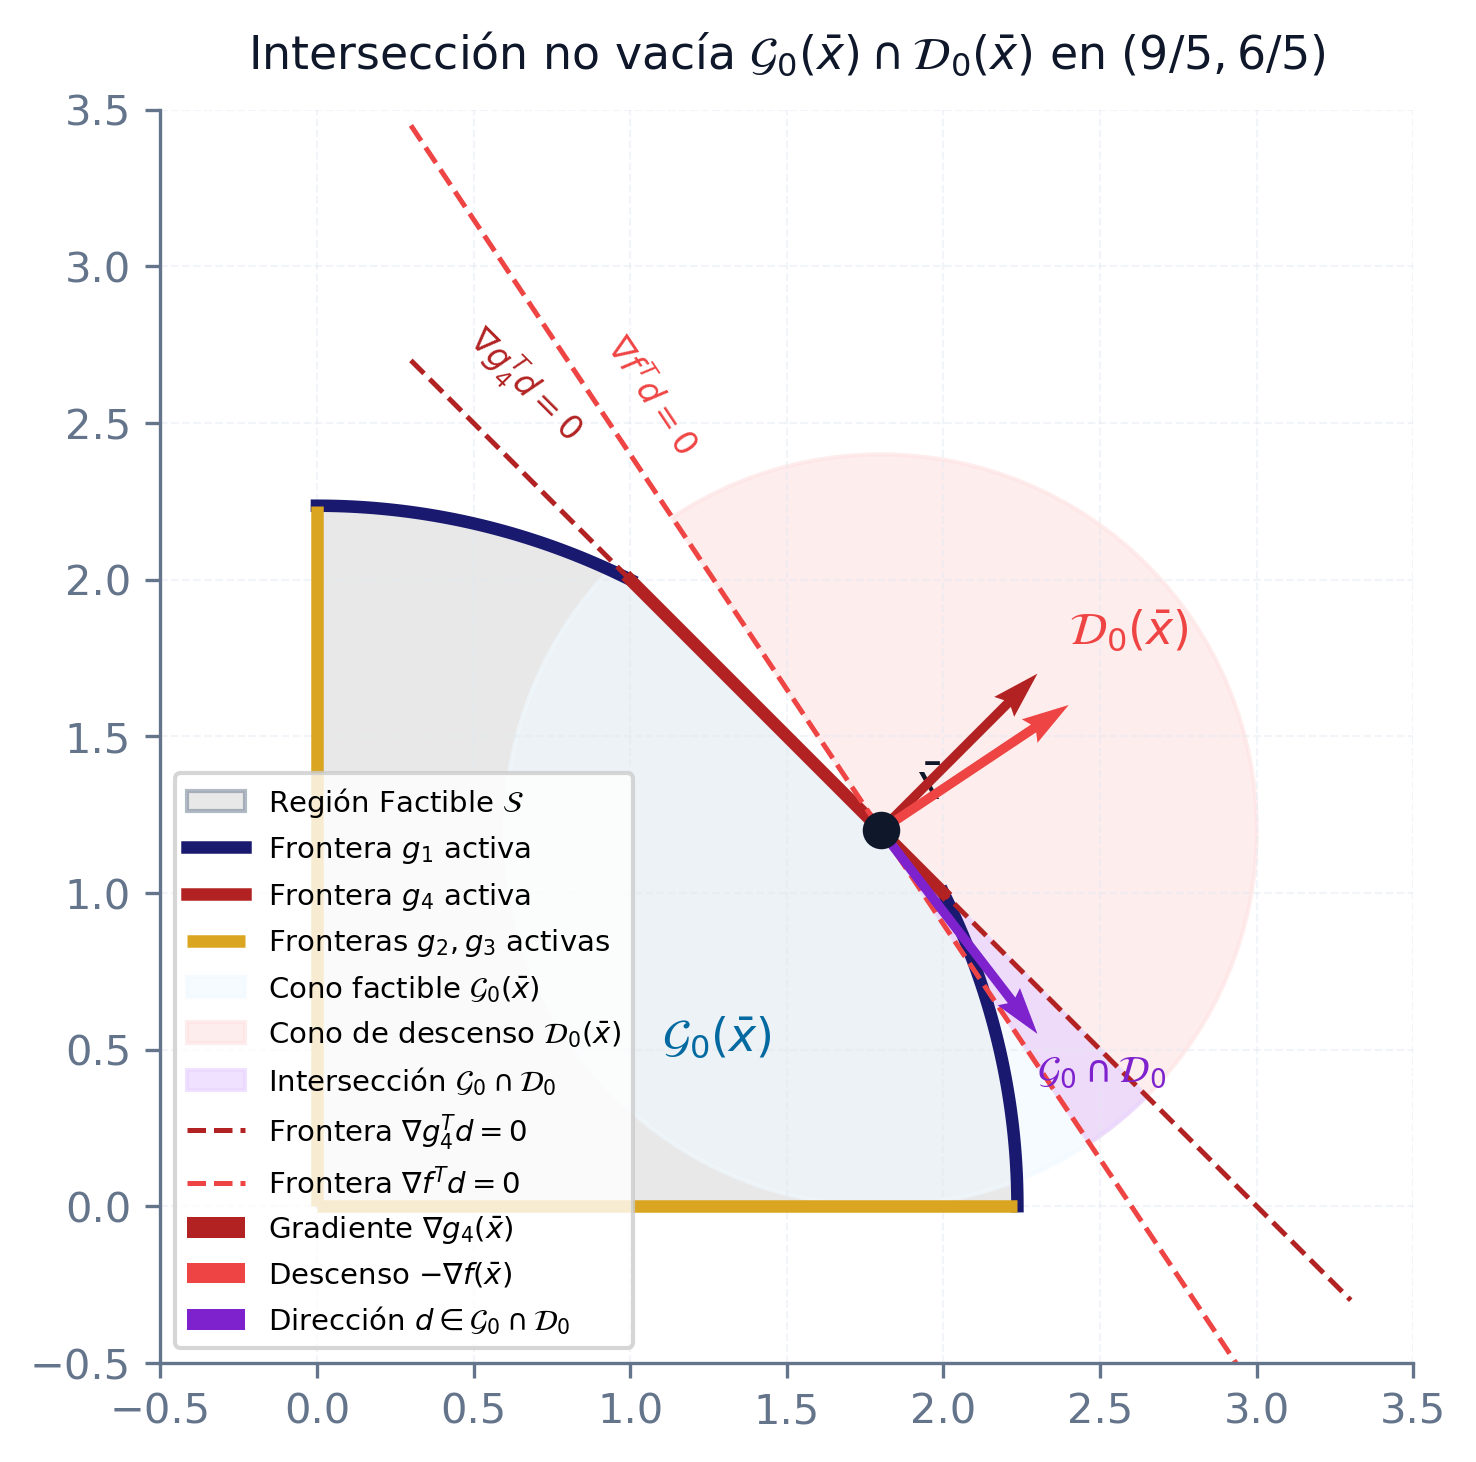
\includegraphics[width=0.6\linewidth,height=\textheight,keepaspectratio]{images/cono_interseccion_no_optimo.png}

  }

  \caption{\label{fig-cono-interseccion-no-optimo}Geometría de conos en
  \(\bar{x} = (9/5, 6/5)\) (no óptimo)}

  \end{figure}%
\item
  \textbf{Punto \(\bar{x} = (2, 1)\)}: Al evaluar las restricciones en
  este punto:
  \[ g_1(2, 1) = 0 \text{ (activa)}, \quad g_2(2, 1) < 0, \quad g_3(2, 1) < 0, \quad g_4(2, 1) = 0 \text{ (activa)} \]
  El conjunto de índices de restricciones activas es
  \(\mathcal{I} = \{1, 4\}\). Sus gradientes y el de la función objetivo
  son:
  \[ \nabla g_1(\bar{x}) = \begin{pmatrix} 4 \\ 2 \end{pmatrix}, \qquad \nabla g_4(\bar{x}) = \begin{pmatrix} 1 \\ 1 \end{pmatrix}, \qquad \nabla f(\bar{x}) = \begin{pmatrix} -2 \\ -2 \end{pmatrix} \]
  Los conos analíticos en este caso se definen como:
  \[ \mathcal{G}_0(\bar{x}) = \{ d \in \mathbb{R}^2 \mid 2d_1 + d_2 < 0 \text{ y } d_1 + d_2 < 0 \} \]
  \[ \mathcal{D}_0(\bar{x}) = \{ d \in \mathbb{R}^2 \mid -\nabla f(\bar{x})^T d > 0 \} = \{ d \in \mathbb{R}^2 \mid d_1 + d_2 > 0 \} \]
  Nótese que cualquier dirección factible algebraica
  \(d \in \mathcal{G}_0(\bar{x})\) debe verificar en particular que
  \(d_1 + d_2 < 0\), lo que implica la inclusión
  \(\mathcal{G}_0(\bar{x}) \subseteq \{d \in \mathbb{R}^2 \mid d_1+d_2 < 0\}\).
  Al ser el cono de descenso
  \(\mathcal{D}_0(\bar{x}) = \{d \in \mathbb{R}^2 \mid d_1+d_2 > 0\}\),
  se hace evidente que ambos conos son mutuamente excluyentes (separados
  por la recta frontera \(d_1+d_2 = 0\)).

  Por lo tanto, la intersección es vacía:
  \[ \mathcal{D}_0(\bar{x}) \cap \mathcal{G}_0(\bar{x}) = \emptyset \]
  Como se ilustra en la Figura~\ref{fig-cono-interseccion-optimo}, los
  conos representados en el espacio de direcciones son disjuntos, lo que
  califica a \(\bar{x} = (2,1)\) como candidato a óptimo.

  \begin{figure}[H]

  \centering{

  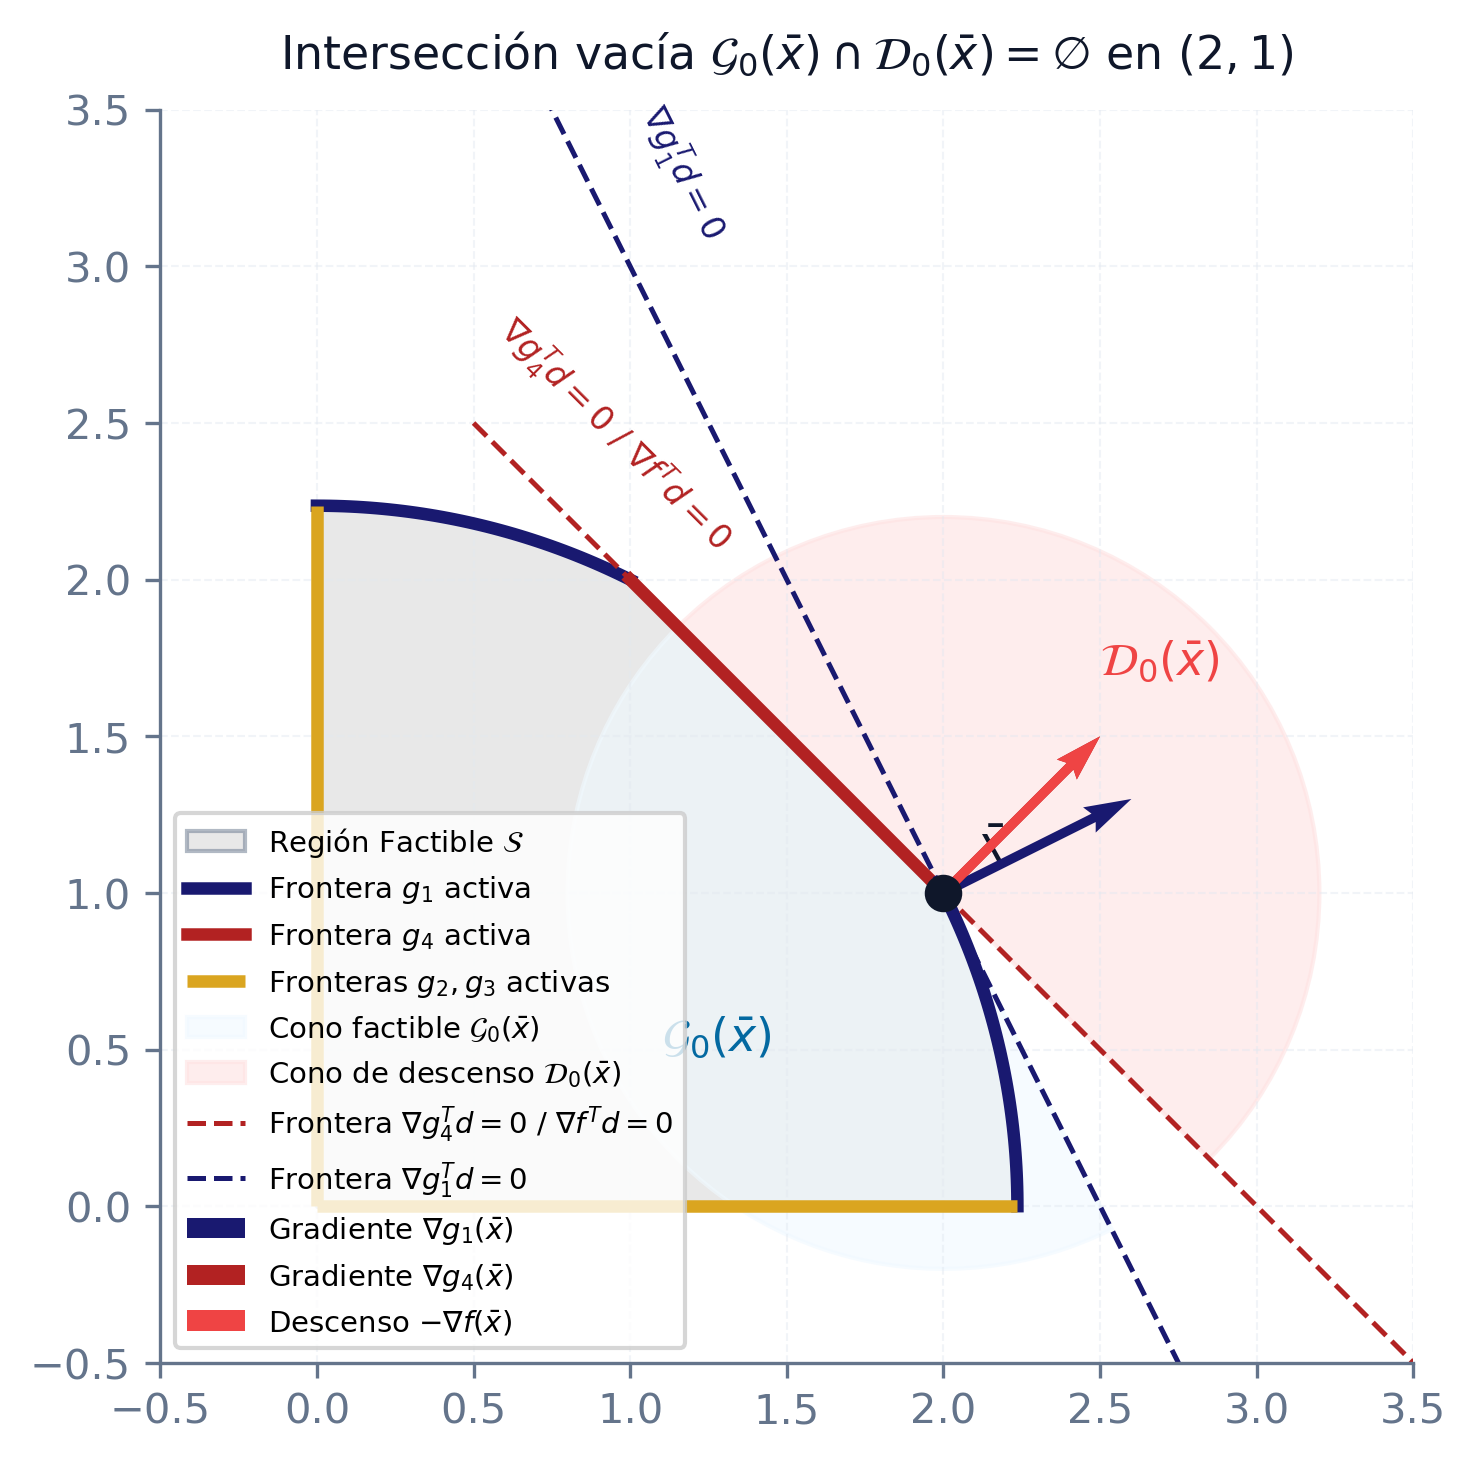
\includegraphics[width=0.6\linewidth,height=\textheight,keepaspectratio]{images/cono_interseccion_optimo.png}

  }

  \caption{\label{fig-cono-interseccion-optimo}Geometría de conos en
  \(\bar{x} = (2, 1)\) (óptimo)}

  \end{figure}%

  \textbf{Nota:} En este punto no se cumple la condición del Teorema de
  Suficiencia geométrica sin KKT, debido a que la restricción lineal
  activa \(g_4(x) = x_1+x_2-3 \le 0\) no es \emph{estrictamente}
  pseudo-convexa (las funciones lineales son pseudo-convexas pero no
  estrictamente pseudo-convexas, ya que admiten puntos distintos con el
  mismo valor de la función y gradientes ortogonales al vector de
  desplazamiento). Sin embargo, al tratarse de un problema con objetivo
  estrictamente convexo y región factible convexa (intersección de
  conjuntos convexos), la condición necesaria de intersección vacía de
  conos es también suficiente para garantizar que \(\bar{x} = (2,1)\) es
  el mínimo global y único del problema.
\end{itemize}

\end{tcolorbox}

\begin{tcolorbox}[enhanced jigsaw, toprule=.15mm, opacitybacktitle=0.6, coltitle=black, colbacktitle=quarto-callout-tip-color!10!white, title=\textcolor{quarto-callout-tip-color}{\faLightbulb}\hspace{0.5em}{Ejemplo: Caso singular de tangencia cúbica}, arc=.35mm, rightrule=.15mm, toptitle=1mm, breakable, bottomtitle=1mm, titlerule=0mm, colback=white, opacityback=0, leftrule=.75mm, colframe=quarto-callout-tip-color-frame, left=2mm, bottomrule=.15mm]

Considérese el siguiente problema: \[
\begin{aligned}
\min \quad & f(x_1, x_2) = (x_1 - 1)^2 + (x_2 - 1)^2 \\
\text{s.a.} \quad & g_1(x_1, x_2) = (x_1 + x_2 - 1)^3 \le 0 \\
& g_2(x_1, x_2) = -x_1 \le 0 \\
& g_3(x_1, x_2) = -x_2 \le 0
\end{aligned}
\] La región factible geométrica de este problema es el triángulo
\(\mathcal{S} = \{ (x_1, x_2) \in \mathbb{R}^2 \mid x_1 + x_2 \le 1, \ x_1 \ge 0, \ x_2 \ge 0 \}\).
Al ser \(f\) estrictamente convexa (las curvas de nivel son
circunferencias concéntricas con centro en \((1,1)\)) y la región
factible convexa, existe un único mínimo global. Geométricamente, el
punto factible más cercano al óptimo no restringido \((1,1)\) es el
punto medio de la hipotenusa (como se muestra en la
Figura~\ref{fig-tangencia-cubica-region}):
\[ \bar{x} = \left(\frac{1}{2}, \frac{1}{2}\right) \]

\begin{figure}[H]

\centering{

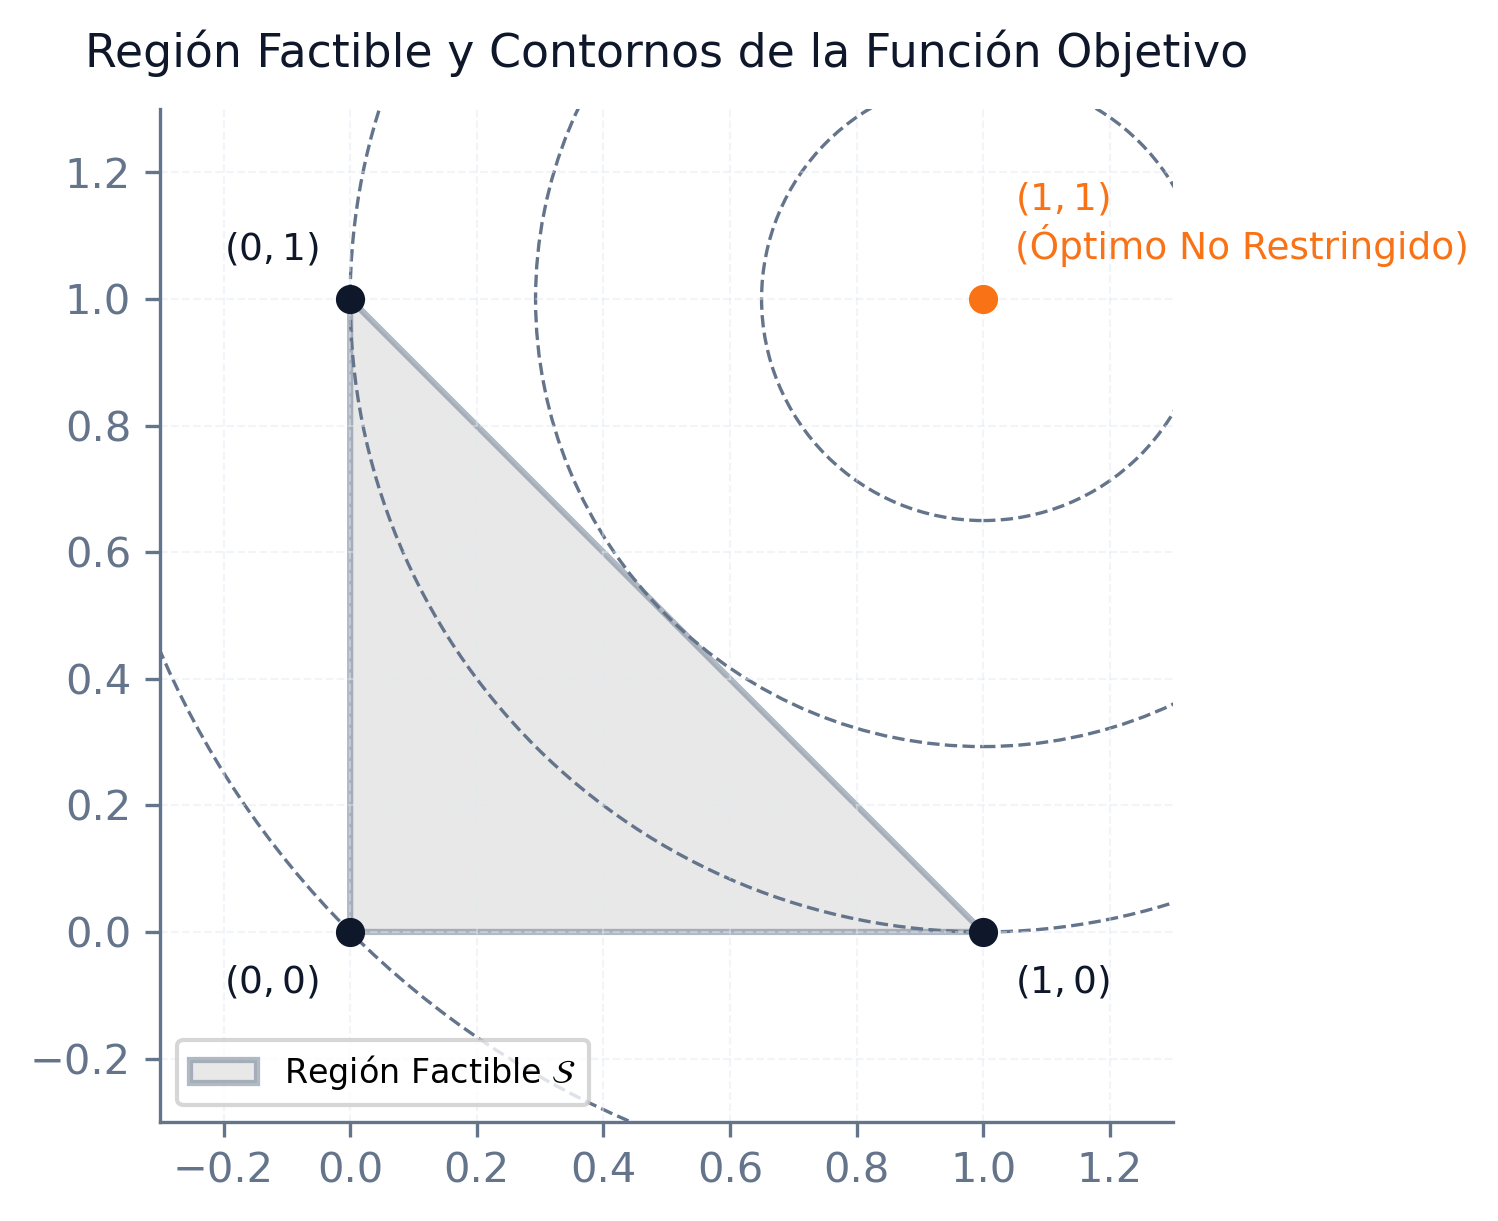
\includegraphics[width=0.6\linewidth,height=\textheight,keepaspectratio]{images/tangencia_cubica_region.png}

}

\caption{\label{fig-tangencia-cubica-region}Visualización de la región
factible y contornos para la tangencia cúbica}

\end{figure}%

En todos los puntos de la frontera definidos por la recta
\(x_1 + x_2 = 1\), la primera restricción es activa (\(g_1(x) = 0\)).
Evaluemos el gradiente de esta restricción activa en cualquier punto de
dicha recta:
\[ \nabla g_1(x_1, x_2) = \begin{pmatrix} 3(x_1 + x_2 - 1)^2 \\ 3(x_1 + x_2 - 1)^2 \end{pmatrix} \]
Puesto que en la recta se cumple \(x_1 + x_2 - 1 = 0\), el gradiente se
anula idénticamente para todos los puntos de la misma:
\[ \nabla g_1(x_1, x_2) = \begin{pmatrix} 0 \\ 0 \end{pmatrix}, \quad \forall (x_1, x_2) \text{ tal que } x_1 + x_2 = 1 \]
En consecuencia, para cualquier punto \(\bar{x}\) sobre esta frontera
(incluyendo puntos no óptimos como el \((1,0)\) o el \((0,1)\)), el cono
de restricciones activas algebraico resulta:
\[ \mathcal{G}_0(\bar{x}) = \{ d \in \mathbb{R}^2 \mid \nabla g_1(\bar{x})^T d < 0 \} = \{ d \in \mathbb{R}^2 \mid 0 < 0 \} = \emptyset \]
Al ser \(\mathcal{G}_0(\bar{x})\) el conjunto vacío, se cumple de manera
trivial que:
\[ \mathcal{D}_0(\bar{x}) \cap \mathcal{G}_0(\bar{x}) = \emptyset \]
para \textbf{todos} los puntos de la recta \(x_1 + x_2 = 1\). Esto
ilustra que la condición necesaria de optimalidad
\(\mathcal{D}_0(\bar{x}) \cap \mathcal{G}_0(\bar{x}) = \emptyset\) se
satisface trivialmente en puntos que no son mínimos, perdiendo toda su
capacidad selectiva debido al carácter singular de la restricción
(tangencia cúbica).

Sin embargo, si reescribimos algebraicamente la región factible con una
restricción equivalente pero de primer orden:
\[ g_1(x_1, x_2) = x_1 + x_2 - 1 \le 0 \] su gradiente pasa a ser
\(\nabla g_1(x_1, x_2) = (1, 1)^T \neq (0,0)^T\). Bajo esta nueva
formulación:
\[ \mathcal{G}_0(\bar{x}) = \{ d \in \mathbb{R}^2 \mid d_1 + d_2 < 0 \} \]
y el cono de descenso es:
\[ \mathcal{D}_0(\bar{x}) = \{ d \in \mathbb{R}^2 \mid 2(x_1 - 1)d_1 + 2(x_2 - 1)d_2 < 0 \} \]
Al evaluar la condición de intersección vacía
\(\mathcal{D}_0(\bar{x}) \cap \mathcal{G}_0(\bar{x}) = \emptyset\), esta
se verifica \textbf{únicamente} en el punto \(\bar{x} = (1/2, 1/2)\),
identificando de forma unívoca el mínimo local (como se ilustra en la
Figura~\ref{fig-tangencia-cubica-optimo}).

\begin{figure}[H]

\centering{

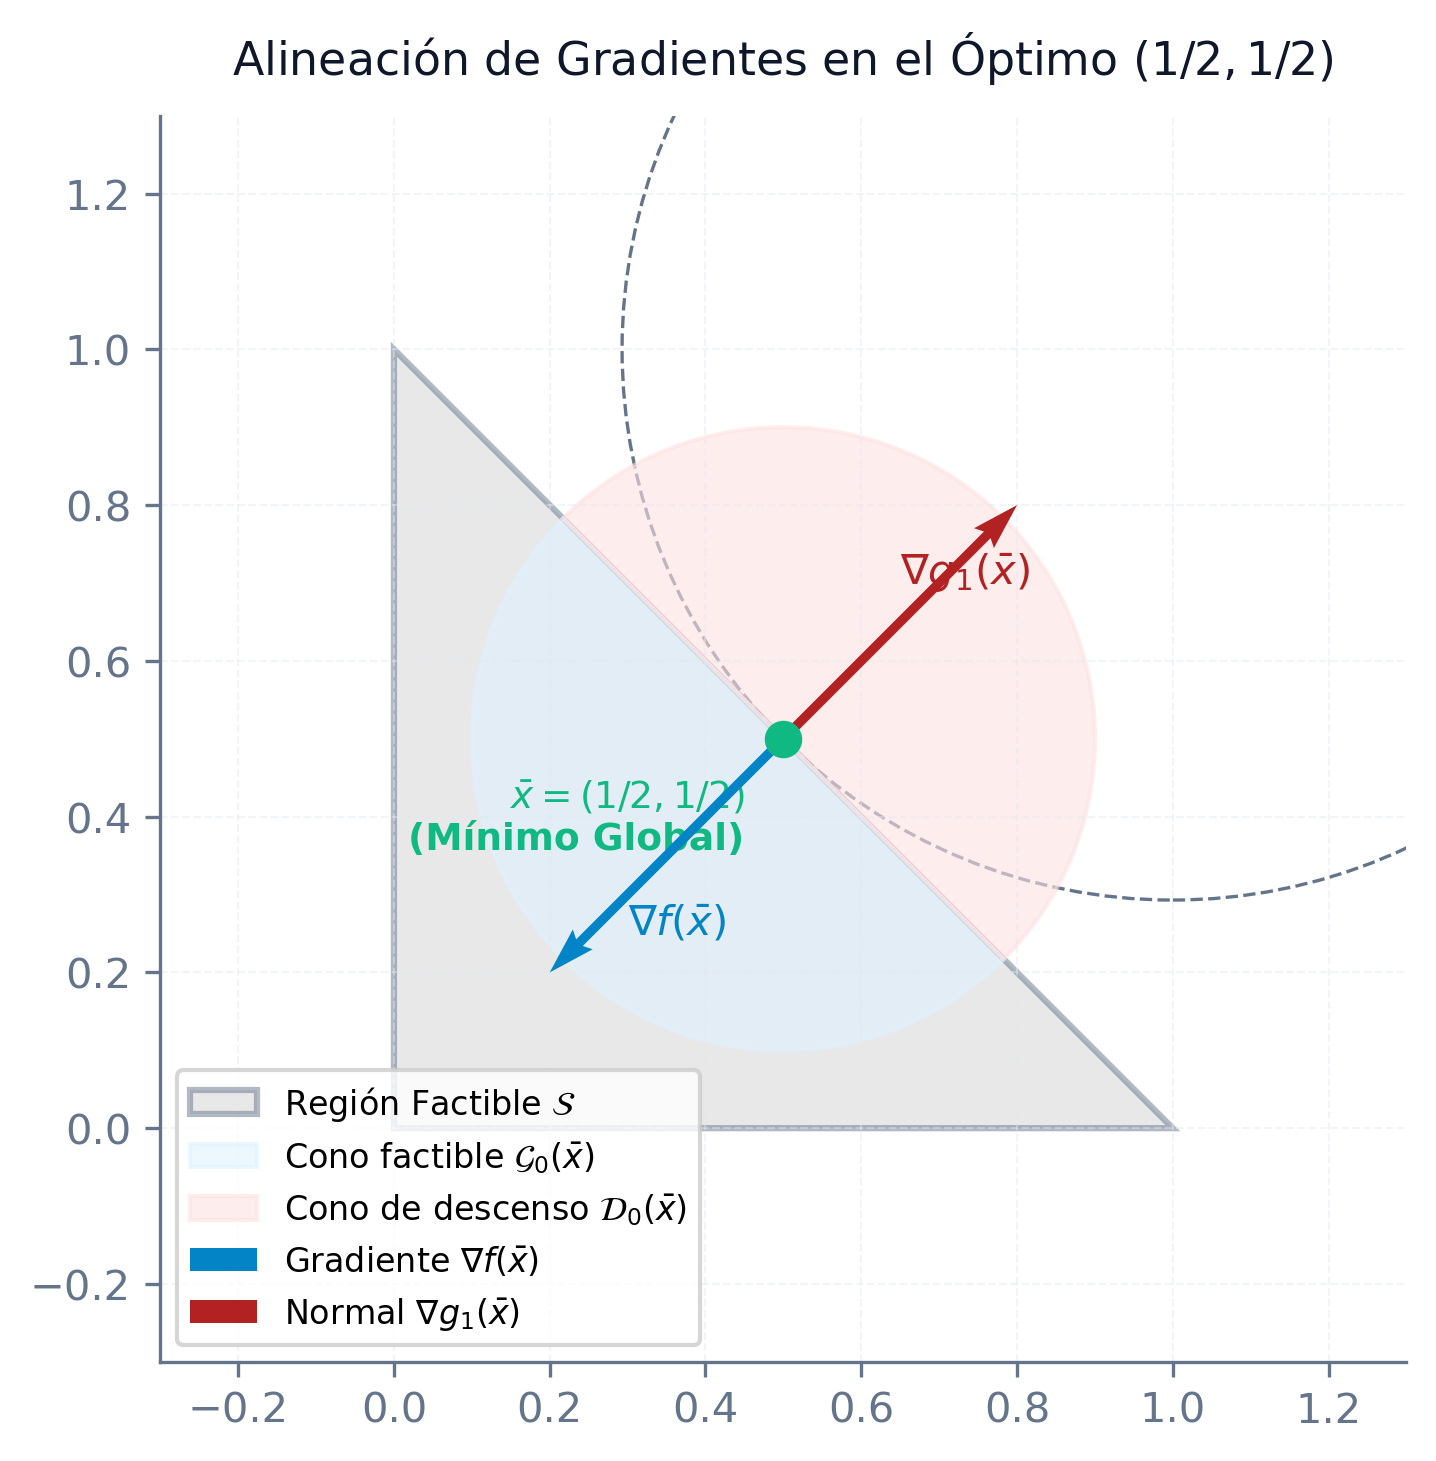
\includegraphics[width=0.6\linewidth,height=\textheight,keepaspectratio]{images/tangencia_cubica_optimo.png}

}

\caption{\label{fig-tangencia-cubica-optimo}Alineación de gradientes en
el óptimo \(\bar{x} = (1/2, 1/2)\) bajo la formulación regularizada}

\end{figure}%

\end{tcolorbox}

\section{Condiciones de Fritz-John
(FJ)}\label{condiciones-de-fritz-john-fj}

La necesidad de encontrar un método algebraico sistemático para
verificar la optimalidad nos lleva a formular el problema de manera
dual. En la sección anterior comprobamos geométricamente que un punto
candidato es óptimo si y solo si la intersección de su cono de descenso
y su cono de restricciones activas es vacía
(\(\mathcal{D}_0(\bar{x}) \cap \mathcal{G}_0(\bar{x}) = \emptyset\)).
Sin embargo, esta verificación directa en el espacio de direcciones
requiere evaluar infinitos vectores, lo cual es impracticable. Para
superar esta limitación, las condiciones de Fritz-John (FJ) traducen
esta exclusión geométrica en un sistema de ecuaciones algebraicas sobre
los gradientes de las funciones, permitiendo comprobar la optimalidad
mediante multiplicadores asociados a cada restricción. Este paso
fundamental se logra formalmente gracias a los lemas de alternativas.

Los lemas de alternativas son resultados clásicos del álgebra lineal y
la convexidad que establecen que de dos sistemas de desigualdades
lineales, uno y solo uno de ellos tiene solución. Permiten asociar
coeficientes (multiplicadores) a las restricciones del problema a partir
de la ausencia de direcciones comunes. Dos de los resultados más
célebres son los siguientes:

\begin{tcolorbox}[enhanced jigsaw, toprule=.15mm, opacitybacktitle=0.6, coltitle=black, colbacktitle=quarto-callout-note-color!10!white, title=\textcolor{quarto-callout-note-color}{\faInfo}\hspace{0.5em}{Lema: Alternativa de Farkas}, arc=.35mm, rightrule=.15mm, toptitle=1mm, breakable, bottomtitle=1mm, titlerule=0mm, colback=white, opacityback=0, leftrule=.75mm, colframe=quarto-callout-note-color-frame, left=2mm, bottomrule=.15mm]

Sean \(A\) una matriz de dimensiones \(m \times n\) y
\(c \in \mathbb{R}^n\). Uno y solo uno de los siguientes sistemas de
restricciones tiene solución:

\begin{enumerate}
\def\labelenumi{\arabic{enumi}.}
\tightlist
\item
  Existe \(x \in \mathbb{R}^n\) tal que \(A x \le 0\) y \(c^T x > 0\).
\item
  Existe \(y \in \mathbb{R}^m\) tal que \(A^T y = c\) e \(y \ge 0\).
\end{enumerate}

\end{tcolorbox}

\begin{tcolorbox}[enhanced jigsaw, toprule=.15mm, opacitybacktitle=0.6, coltitle=black, colbacktitle=quarto-callout-note-color!10!white, title=\textcolor{quarto-callout-note-color}{\faInfo}\hspace{0.5em}{Lema: Alternativa de Gordan}, arc=.35mm, rightrule=.15mm, toptitle=1mm, breakable, bottomtitle=1mm, titlerule=0mm, colback=white, opacityback=0, leftrule=.75mm, colframe=quarto-callout-note-color-frame, left=2mm, bottomrule=.15mm]

Sea \(A\) una matriz de dimensiones \(m \times n\). Uno y solo uno de
los siguientes sistemas de restricciones tiene solución:

\begin{enumerate}
\def\labelenumi{\arabic{enumi}.}
\tightlist
\item
  Existe \(x \in \mathbb{R}^n\) tal que \(A x < 0\).
\item
  Existe \(y \in \mathbb{R}^m\) tal que \(A^T y = 0\), \(y \ge 0\) e
  \(y \neq 0\).
\end{enumerate}

\end{tcolorbox}

La utilidad de estos lemas radica en que nos permiten reformular la
disyunción geométrica en términos de combinaciones lineales de
gradientes. En particular, la condición de optimalidad geométrica exige
que no exista ninguna dirección \(d\) que satisfaga simultáneamente
\(\nabla f(\bar{x})^T d < 0\) y \(\nabla g_i(\bar{x})^T d < 0\) para las
restricciones activas. Si representamos estos gradientes como las filas
de una matriz \(A\), esta condición equivale a afirmar que el sistema de
desigualdades estrictas \(Ad < 0\) no tiene solución. Al aplicar el Lema
de Gordan a este sistema sin solución, este nos garantiza de forma dual
la existencia de un vector de coeficientes no negativos y no todos nulos
que anula la combinación lineal de las filas. De este modo, la ausencia
de una dirección factible de descenso se traduce en la existencia de un
equilibrio de fuerzas entre los gradientes del objetivo y de las
restricciones activas, dando origen al teorema de Fritz-John (John
1948):

\begin{tcolorbox}[enhanced jigsaw, toprule=.15mm, opacitybacktitle=0.6, coltitle=black, colbacktitle=quarto-callout-important-color!10!white, title=\textcolor{quarto-callout-important-color}{\faExclamation}\hspace{0.5em}{Teorema: Condiciones necesarias de Fritz-John (1948)}, arc=.35mm, rightrule=.15mm, toptitle=1mm, breakable, bottomtitle=1mm, titlerule=0mm, colback=white, opacityback=0, leftrule=.75mm, colframe=quarto-callout-important-color-frame, left=2mm, bottomrule=.15mm]

Sea \(\bar{x}\) un mínimo local del problema restringido por
desigualdades. Si \(f\) y las restricciones activas \(g_i\)
(\(i \in \mathcal{I}\)) son diferenciables en \(\bar{x}\), y las
inactivas son continuas, existen escalares \(u_0, u_1, \dots, u_m\)
tales que:

\begin{enumerate}
\def\labelenumi{\arabic{enumi}.}
\tightlist
\item
  \textbf{Factibilidad dual (Ecuación de Fritz-John)}:
  \[ u_0 \nabla f(\bar{x}) + \sum_{i=1}^m u_i \nabla g_i(\bar{x}) = 0 \]
\item
  \textbf{Holgura complementaria}:
  \[ u_i g_i(\bar{x}) = 0, \quad \forall i = 1, \dots, m \]
\item
  \textbf{No negatividad}:
  \[ u_0, u_i \ge 0, \quad \forall i = 1, \dots, m \]
\item
  \textbf{No trivialidad}:
  \[ (u_0, u_1, \dots, u_m) \neq (0, 0, \dots, 0) \]
\end{enumerate}

\emph{Demostración}: Puesto que \(\bar{x}\) es un mínimo local del
problema, se cumple que
\(\mathcal{D}_0(\bar{x}) \cap \mathcal{G}_0(\bar{x}) = \emptyset\). Esto
equivale a afirmar que el sistema de desigualdades estrictas:
\[ \nabla f(\bar{x})^T d < 0 \qquad \text{y} \qquad \nabla g_i(\bar{x})^T d < 0, \quad \forall i \in \mathcal{I} \]
no tiene solución \(d \in \mathbb{R}^n\). Definamos la matriz \(A\)
cuyas filas son \(\nabla f(\bar{x})^T\) y \(\nabla g_i(\bar{x})^T\) para
cada \(i \in \mathcal{I}\). El hecho de que no exista ninguna dirección
\(d\) implica que el sistema lineal \(A d < 0\) no tiene solución.

Aplicando el Lema de Gordan a la matriz \(A\), existe un vector de
multiplicadores no trivial \(p = (u_0, u_{\mathcal{I}})^T \ge 0\) con
\(p \neq 0\) tal que:
\[ A^T p = u_0 \nabla f(\bar{x}) + \sum_{i \in \mathcal{I}} u_i \nabla g_i(\bar{x}) = 0 \]
Definiendo \(u_j = 0\) para todos los índices de restricciones inactivas
(\(j \notin \mathcal{I}\)), se satisfacen de forma automática las
condiciones de holgura complementaria y se obtiene la relación general
para todo \(i = 1, \dots, m\), lo que demuestra el teorema.
\(\blacksquare\)

\end{tcolorbox}

El aspecto clave de este teorema es que introduce el multiplicador
\(u_0\) para la función objetivo. Si \(u_0 > 0\), las condiciones
necesarias de Fritz-John equivalen a las condiciones de
Karush-Kuhn-Tucker (KKT). Sin embargo, si \(u_0 = 0\), el objetivo
desaparece de la ecuación dual y las condiciones se satisfacen de forma
puramente geométrica por la disposición de las restricciones en la
frontera, perdiendo su utilidad para encontrar mínimos.

Para interpretar físicamente este equilibrio de gradientes, resulta de
gran valor analizar cómo actúan y qué significan estos multiplicadores
en el plano coordenado. Dependiendo de la disposición geométrica de las
restricciones y de la orientación de las curvas de nivel del objetivo,
el sistema dual de Fritz-John puede comportarse de maneras muy
distintas. A través del siguiente ejemplo interactivo en el punto de
intersección \((7/3, 4/3)\), exploraremos los cuatro escenarios
fundamentales que caracterizan esta relación dual, comprendiendo cómo
los signos y la dependencia lineal de los gradientes determinan si el
punto es un mínimo regular, un punto redundante con múltiples
multiplicadores, una singularidad de la frontera o un máximo descartado.

\begin{tcolorbox}[enhanced jigsaw, toprule=.15mm, opacitybacktitle=0.6, coltitle=black, colbacktitle=quarto-callout-tip-color!10!white, title=\textcolor{quarto-callout-tip-color}{\faLightbulb}\hspace{0.5em}{Ejemplo: Interpretación geométrica de Fritz-John en cuatro casos}, arc=.35mm, rightrule=.15mm, toptitle=1mm, breakable, bottomtitle=1mm, titlerule=0mm, colback=white, opacityback=0, leftrule=.75mm, colframe=quarto-callout-tip-color-frame, left=2mm, bottomrule=.15mm]

Consideremos el punto de intersección \(\bar{x} = (7/3, 4/3)\) bajo
diferentes problemas de optimización con restricciones lineales activas
\(g_1(x, y) = 2x+y-6 \le 0\) y \(g_2(x, y) = x-y-1 \le 0\), cuyos
gradientes en \(\bar{x}\) son \(\nabla g_1 = (2, 1)^T\) y
\(\nabla g_2 = (1, -1)^T\). Analizaremos la relación entre el gradiente
del objetivo \(\nabla f(\bar{x})\), el opuesto \(-\nabla f(\bar{x})\) y
los gradientes de las restricciones en cuatro escenarios.

\textbf{Caso 1: Restricciones Linealmente Independientes (Mínimo Local
Regular)} Estudiamos la minimización de \(f(x, y) = (x-5)^2+(y-1)^2\)
sujeto a \(g_1\) y \(g_2\). El opuesto del gradiente del objetivo en
\(\bar{x}\) es \(-\nabla f(\bar{x}) = (16/3, -2/3)^T\), el cual se
encuentra dentro del cono convexo generado por los gradientes de las
restricciones activas (véase la Figura~\ref{fig-fj-caso1-li}). Al
resolver la ecuación dual:
\[ u_0 \begin{pmatrix} 16/3 \\ -2/3 \end{pmatrix} = u_1 \begin{pmatrix} 2 \\ 1 \end{pmatrix} + u_2 \begin{pmatrix} 1 \\ -1 \end{pmatrix} \]
obtenemos la solución única en función de \(u_0\):
\(u_1 = \frac{14}{9}u_0 > 0\) y \(u_2 = \frac{20}{9}u_0 > 0\). Al poder
fijar \(u_0 = 1\), el punto es un mínimo regular válido.

\begin{figure}[H]

\centering{

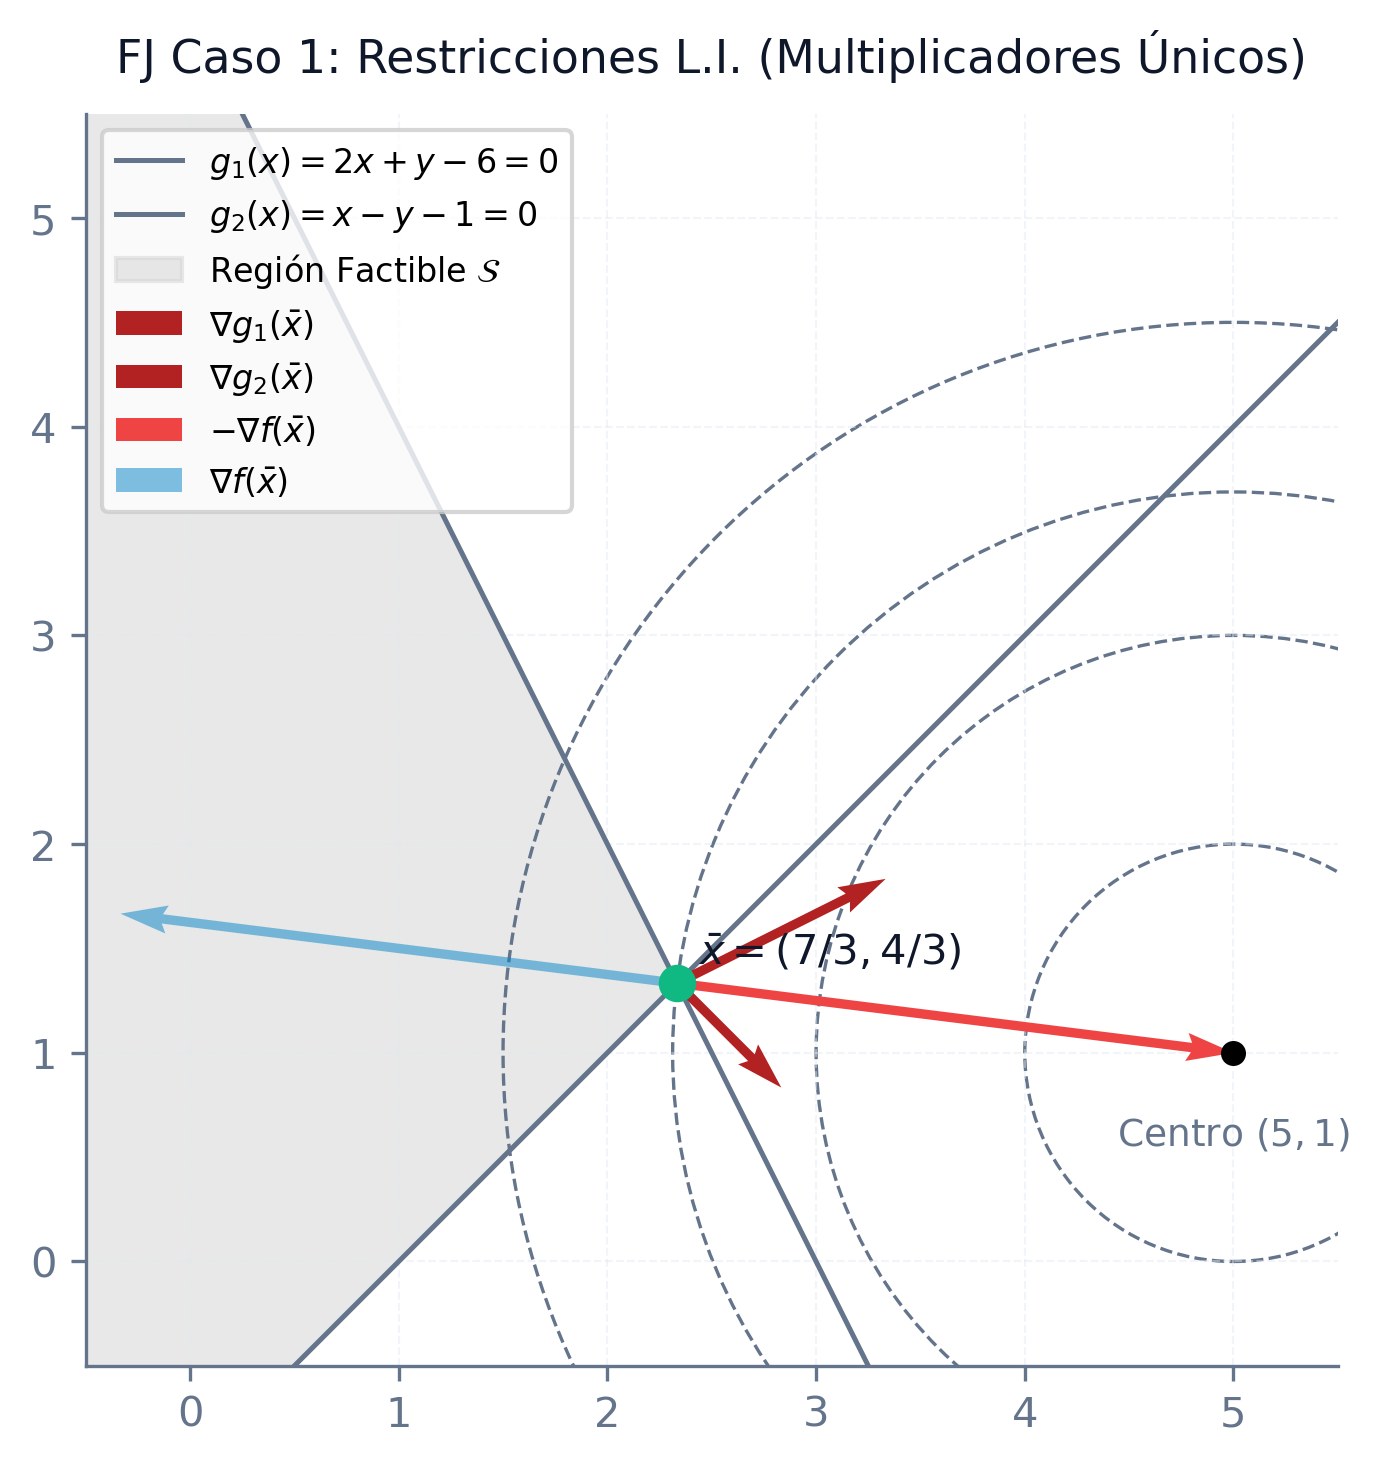
\includegraphics[width=0.6\linewidth,height=\textheight,keepaspectratio]{images/fj_caso1_li.png}

}

\caption{\label{fig-fj-caso1-li}FJ Caso 1: Restricciones linealmente
independientes y \(-\nabla f(\bar{x})\) dentro del cono factible}

\end{figure}%

\textbf{Caso 2: Restricción Activa Redundante (Linealmente Dependiente)}
Añadimos al problema anterior la restricción redundante
\(g_3(x, y) = x \le 7/3\), activa en \(\bar{x}\) con gradiente
\(\nabla g_3 = (1, 0)^T\). Como se ilustra en la
Figura~\ref{fig-fj-caso2-redundante}, los tres gradientes de las
restricciones son linealmente dependientes. La ecuación dual admite
infinitas combinaciones válidas para expresar \(-\nabla f(\bar{x})\).
Por ejemplo, con \(u_0 = 1\), la familia de soluciones está dada por
\(u_1 \in [0, 14/9]\), \(u_2 = u_1 + 2/3\), y \(u_3 = 14/3 - 3u_1\),
perdiendo la unicidad de los multiplicadores.

\begin{figure}[H]

\centering{

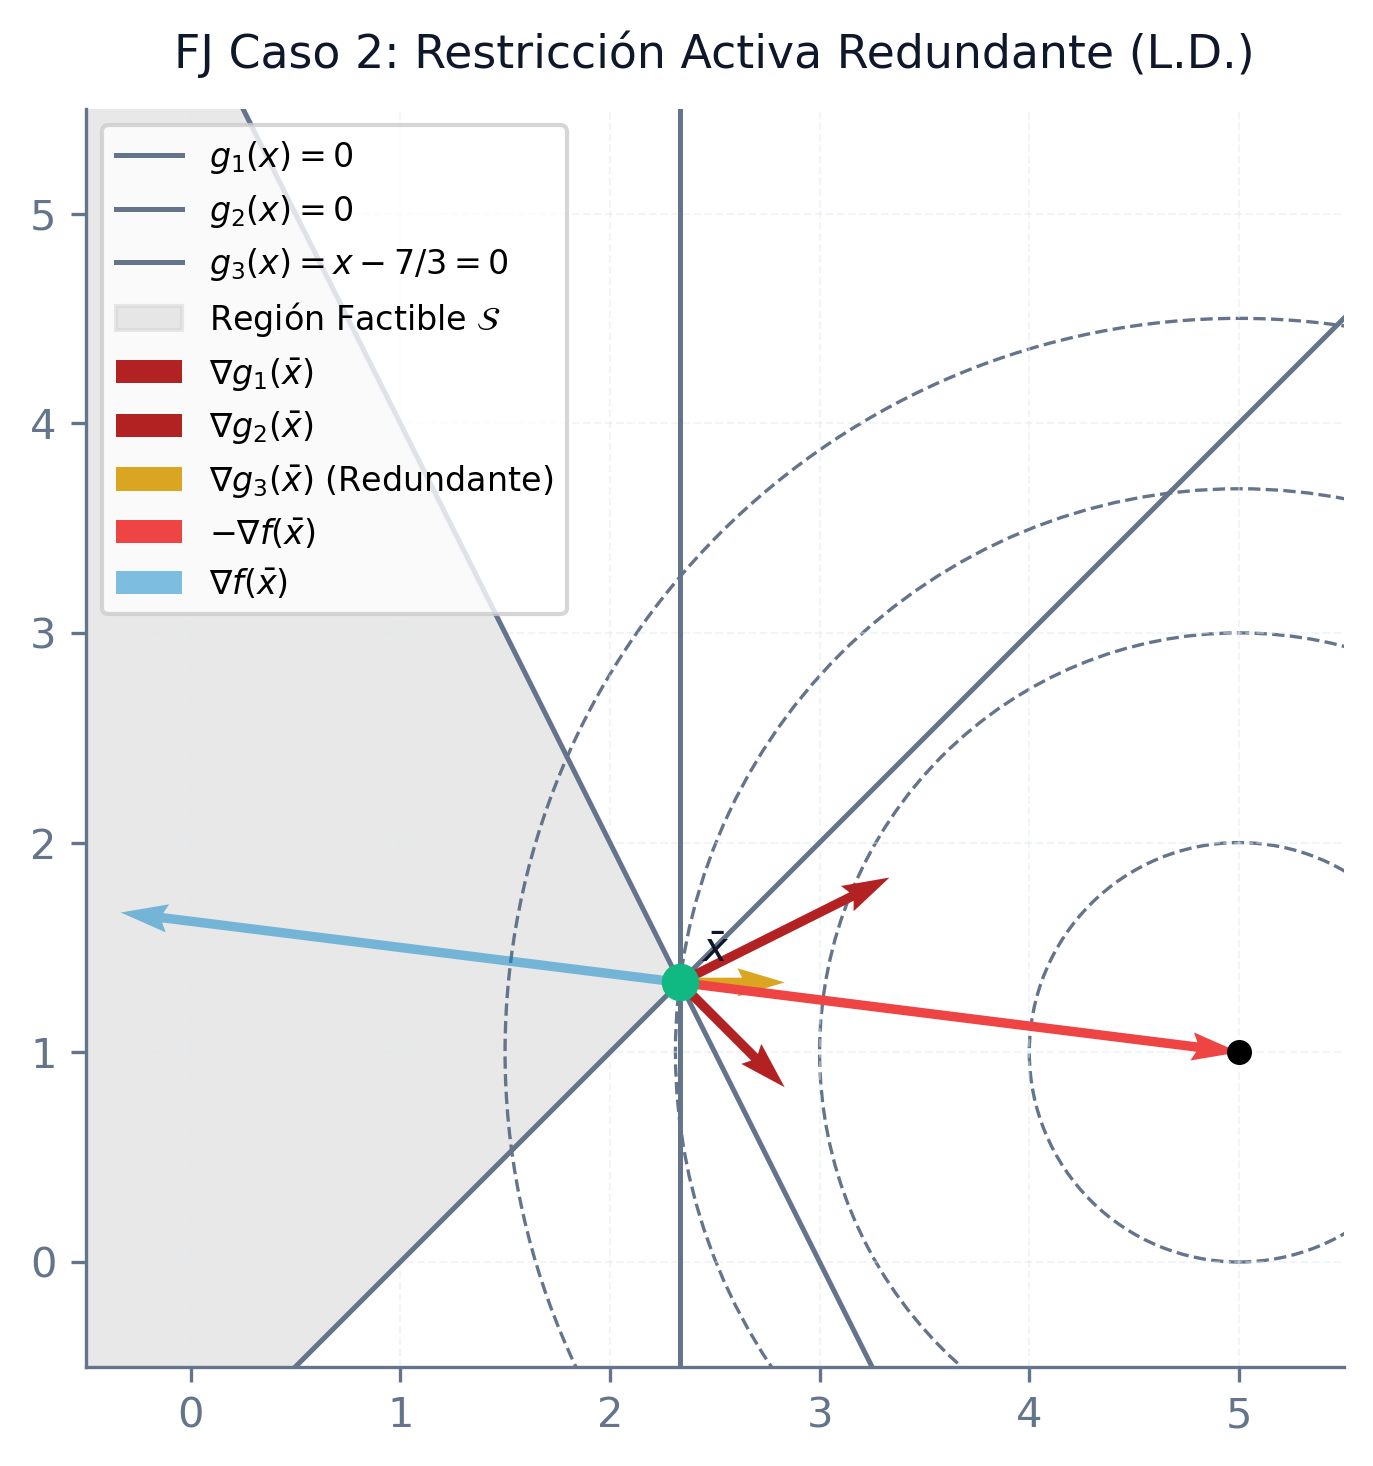
\includegraphics[width=0.6\linewidth,height=\textheight,keepaspectratio]{images/fj_caso2_redundante.png}

}

\caption{\label{fig-fj-caso2-redundante}FJ Caso 2: Restricción activa
redundante y pérdida de la unicidad de los multiplicadores}

\end{figure}%

\textbf{Caso 3: Conos de Restricción Contradictorios (Singularidad con
\(u_0 = 0\))} Añadimos la restricción opuesta
\(g_3(x, y) = -x \le -7/3\), con gradiente \(\nabla g_3 = (-1, 0)^T\).
Los tres gradientes activos cubren el espacio imposibilitando cualquier
dirección factible (\(\mathcal{G}_0 = \emptyset\)). En este caso, la
Figura~\ref{fig-fj-caso3-contradictorio} muestra que podemos equilibrar
los gradientes de las restricciones de forma interna sin la
participación del objetivo:
\[ u_1 \begin{pmatrix} 2 \\ 1 \end{pmatrix} + u_2 \begin{pmatrix} 1 \\ -1 \end{pmatrix} + u_3 \begin{pmatrix} -1 \\ 0 \end{pmatrix} = \begin{pmatrix} 0 \\ 0 \end{pmatrix} \implies u_1 = u_2 = 1, \ u_3 = 3 \]
Esto nos da una solución no trivial con \(u_0 = 0\), \(u_1 = 1\),
\(u_2 = 1\), \(u_3 = 3\). Las condiciones FJ se cumplen de forma trivial
e independiente del objetivo.

\begin{figure}[H]

\centering{

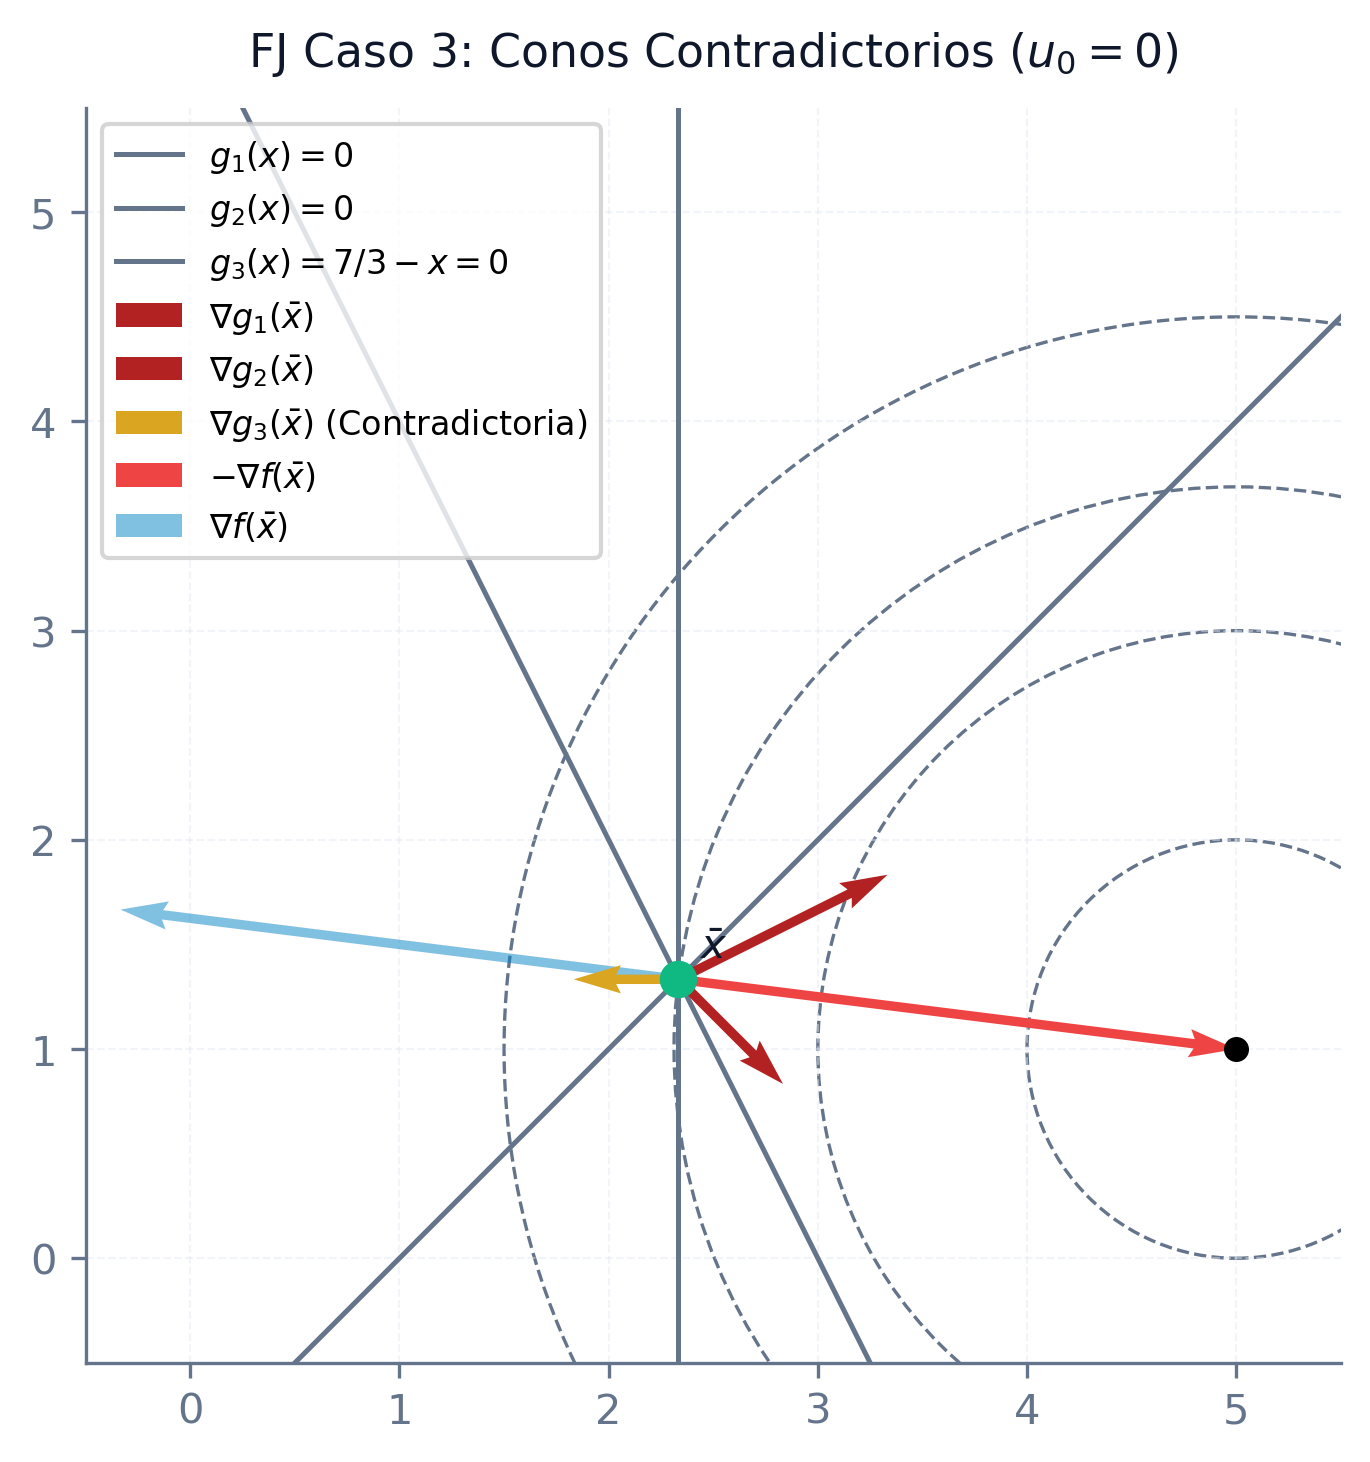
\includegraphics[width=0.6\linewidth,height=\textheight,keepaspectratio]{images/fj_caso3_contradictorio.png}

}

\caption{\label{fig-fj-caso3-contradictorio}FJ Caso 3: Conos de
restricción contradictorios que provocan \(u_0 = 0\)}

\end{figure}%

\textbf{Caso 4: Punto de Máximo Local (Multiplicadores Negativos)} Si
intentamos minimizar \(f(x, y) = -(x-5)^2-(y-1)^2\) (o equivalentemente,
maximizar la distancia a \((5,1)\)), el opuesto del gradiente apunta
hacia fuera del cono generado por los gradientes de las restricciones
activas: \(-\nabla f(\bar{x}) = (-16/3, 2/3)^T\) (véase la
Figura~\ref{fig-fj-caso4-maximo}). Al resolver la ecuación dual con
\(u_0 > 0\), los multiplicadores resultan negativos
(\(u_1 = -14/9u_0 < 0\)), lo que permite descartar correctamente este
candidato a mínimo local.

\begin{figure}[H]

\centering{

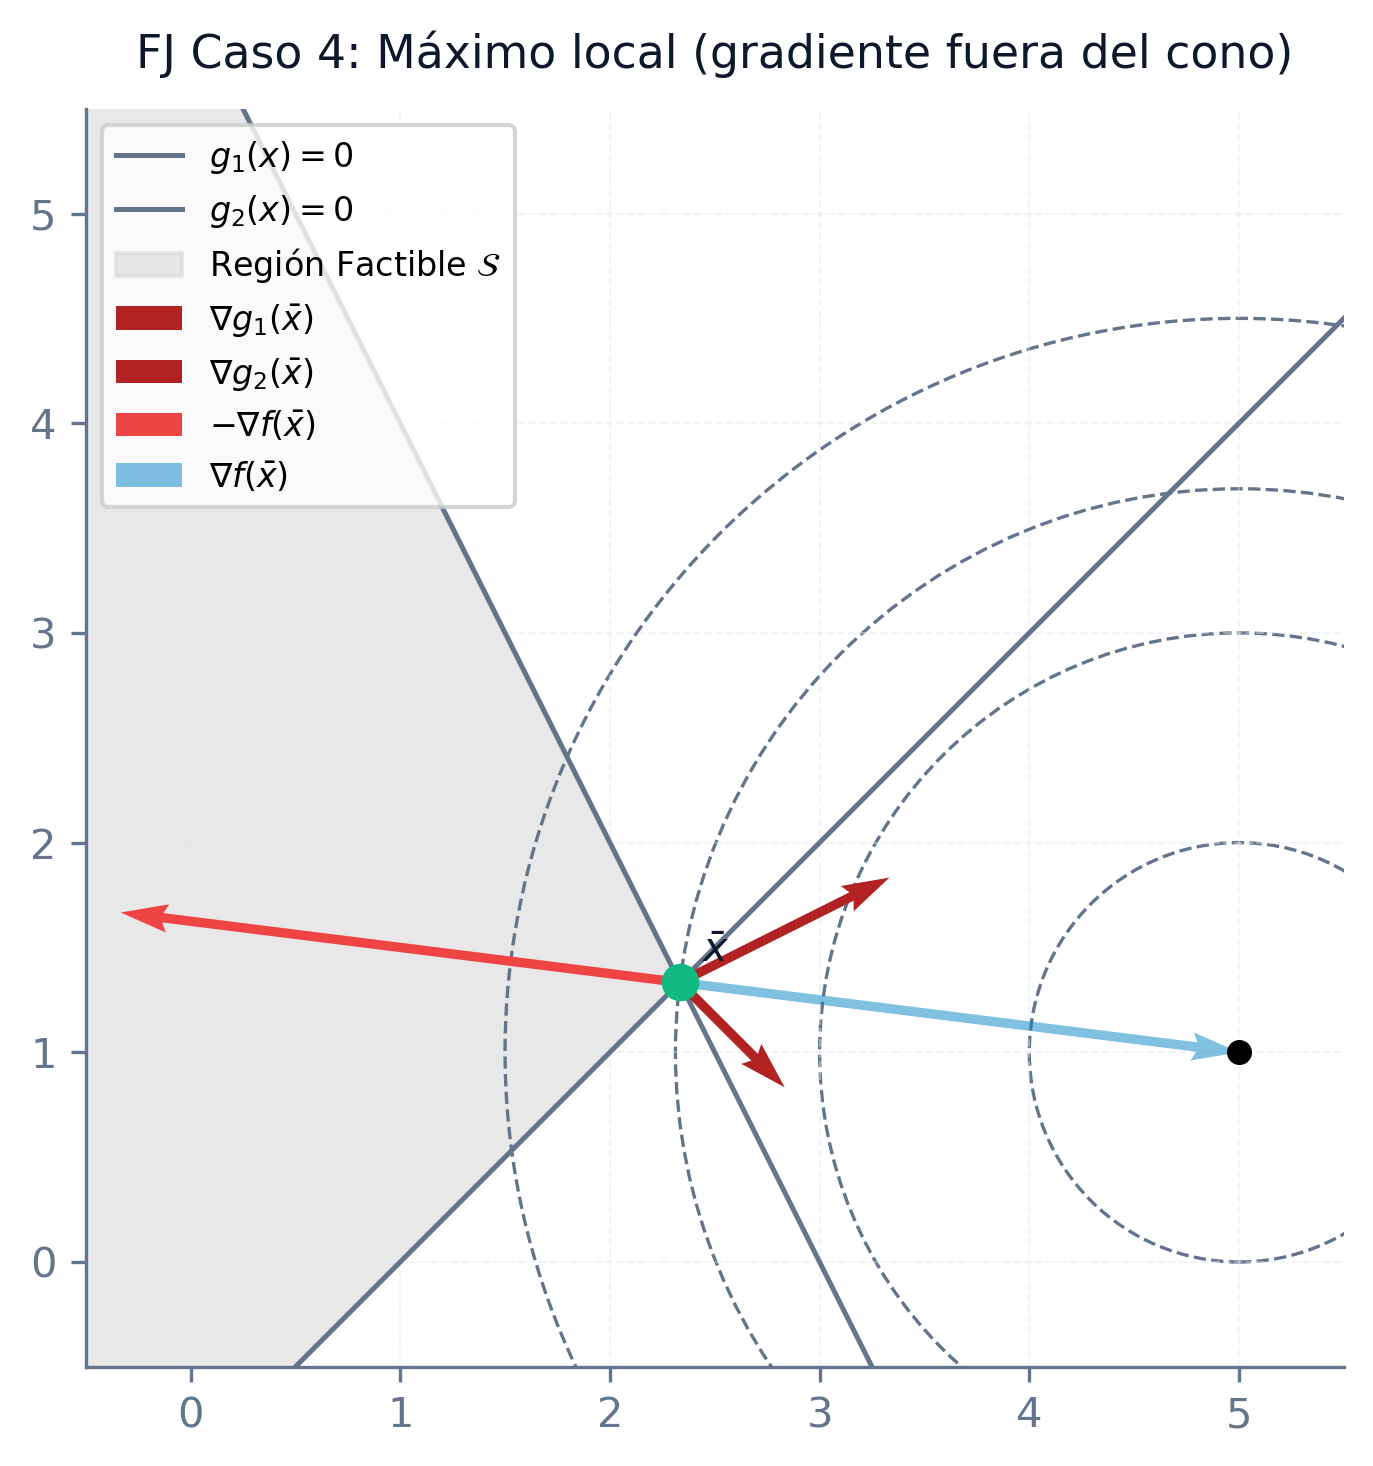
\includegraphics[width=0.6\linewidth,height=\textheight,keepaspectratio]{images/fj_caso4_maximo.png}

}

\caption{\label{fig-fj-caso4-maximo}FJ Caso 4: Dirección del gradiente
opuesta y descarte de un máximo local}

\end{figure}%

\end{tcolorbox}

El análisis de estos cuatro casos revela que las condiciones de
Fritz-John no solo identifican mínimos locales regulares, sino que
actúan como un ``filtro'' analítico que captura cualquier punto singular
de la frontera de la región factible, independientemente de la función
objetivo. Esto nos permite clasificar los candidatos seleccionados por
el formalismo dual de Fritz-John en tres grandes familias según su
origen físico y geométrico:

\begin{enumerate}
\def\labelenumi{\arabic{enumi}.}
\tightlist
\item
  \textbf{Vértices o puntos de esquina}: Puntos de la frontera donde
  coinciden múltiples restricciones activas linealmente independientes
  que bloquean cualquier dirección de movimiento físico,
  independientemente de la dirección de la función objetivo.
\item
  \textbf{Puntos de tangencia regular}: Puntos de la frontera lisa de
  una restricción donde el gradiente de la función objetivo
  \(\nabla f(\bar{x})\) y el gradiente de la restricción activa
  \(\nabla g_i(\bar{x})\) son colineales y apuntan en sentidos opuestos,
  cumpliendo directamente la condición de tangencia con \(u_0 > 0\).
\item
  \textbf{Puntos singulares o de cúspide}: Puntos donde la geometría de
  la frontera es tan restrictiva que la cualificación de restricciones
  falla (los gradientes activos son linealmente dependientes),
  permitiendo resolver el sistema con \(u_0 = 0\) sin importar cómo se
  comporte localmente la función objetivo.
\end{enumerate}

Esta capacidad para identificar singularidades es a la vez una virtud y
una debilidad del formalismo de Fritz-John. En puntos singulares, el
sistema dual se satisface de forma espuria con un multiplicador de la
función objetivo nulo (\(u_0 = 0\)), lo que significa que el gradiente
de la función que deseamos minimizar no ejerce ninguna influencia en las
ecuaciones de optimalidad. Este fenómeno de insensibilidad se vuelve
evidente cuando la frontera presenta tangencias singulares o cuando se
introducen restricciones redundantes artificiales, como se analiza en la
siguiente advertencia teórica:

\begin{tcolorbox}[enhanced jigsaw, toprule=.15mm, opacitybacktitle=0.6, coltitle=black, colbacktitle=quarto-callout-warning-color!10!white, title=\textcolor{quarto-callout-warning-color}{\faExclamationTriangle}\hspace{0.5em}{Nota teórica sobre vulnerabilidad por redundancia trivial}, arc=.35mm, rightrule=.15mm, toptitle=1mm, breakable, bottomtitle=1mm, titlerule=0mm, colback=white, opacityback=0, leftrule=.75mm, colframe=quarto-callout-warning-color-frame, left=2mm, bottomrule=.15mm]

Es importante notar que siempre es posible transformar de forma
artificial cualquier punto factible en un candidato Fritz-John añadiendo
una restricción redundante inútil. Por ejemplo, si añadimos la
restricción \(\|x - \bar{x}\| \ge 0\), que es universalmente cierta, en
el punto \(\bar{x}\) esta restricción se activa y su gradiente es nulo.
Esto provoca que el cono de restricciones active \(\mathcal{G}_0\) se
vuelva vacío, forzando a que las condiciones de Fritz-John se satisfagan
de manera trivial con multiplicadores no nulos e \(u_0 = 0\).

\end{tcolorbox}

Para ilustrar este comportamiento patológico y entender cómo se rompe la
sensibilidad del objetivo, analizaremos detalladamente un problema con
una tangencia de orden superior (cúbica) en la frontera, donde el
multiplicador de la función objetivo se anula obligatoriamente en el
óptimo:

\begin{tcolorbox}[enhanced jigsaw, toprule=.15mm, opacitybacktitle=0.6, coltitle=black, colbacktitle=quarto-callout-tip-color!10!white, title=\textcolor{quarto-callout-tip-color}{\faLightbulb}\hspace{0.5em}{Ejemplo: Fallo de Fritz-John por multiplicador nulo}, arc=.35mm, rightrule=.15mm, toptitle=1mm, breakable, bottomtitle=1mm, titlerule=0mm, colback=white, opacityback=0, leftrule=.75mm, colframe=quarto-callout-tip-color-frame, left=2mm, bottomrule=.15mm]

Consideremos el problema: \[
\begin{aligned}
\min_{x} \quad & -x_1 \\
\text{sujeto a} \quad & g_1(x_1, x_2) = x_2 - (1 - x_1)^3 \le 0 \\
& g_2(x_1, x_2) = -x_2 \le 0
\end{aligned}
\] La solución óptima de este problema es \(\bar{x} = (1, 0)\) (como se
ilustra en la Figura~\ref{fig-fj-ejemplo-cuba}), donde ambas
restricciones son activas (\(\mathcal{I} = \{1, 2\}\)). Planteando las
ecuaciones de Fritz-John:
\[ u_0 \begin{pmatrix} -1 \\ 0 \end{pmatrix} + u_1 \begin{pmatrix} 3(1 - x_1)^2 \\ 1 \end{pmatrix} + u_2 \begin{pmatrix} 0 \\ -1 \end{pmatrix} = \begin{pmatrix} 0 \\ 0 \end{pmatrix} \]
Evaluando en el punto óptimo \(\bar{x} = (1, 0)\):
\[ u_0 \begin{pmatrix} -1 \\ 0 \end{pmatrix} + u_1 \begin{pmatrix} 0 \\ 1 \end{pmatrix} + u_2 \begin{pmatrix} 0 \\ -1 \end{pmatrix} = \begin{pmatrix} 0 \\ 0 \end{pmatrix} \implies \begin{aligned} -u_0 &= 0 \\ u_1 - u_2 &= 0 \end{aligned} \]
De donde se deduce obligatoriamente que \(u_0 = 0\), e
\(u_1 = u_2 = \alpha > 0\). La función objetivo no influye en las
ecuaciones debido a la geometría singular de la región factible en dicho
punto (la tangencia de las curvas de restricción).

\begin{figure}[H]

\centering{

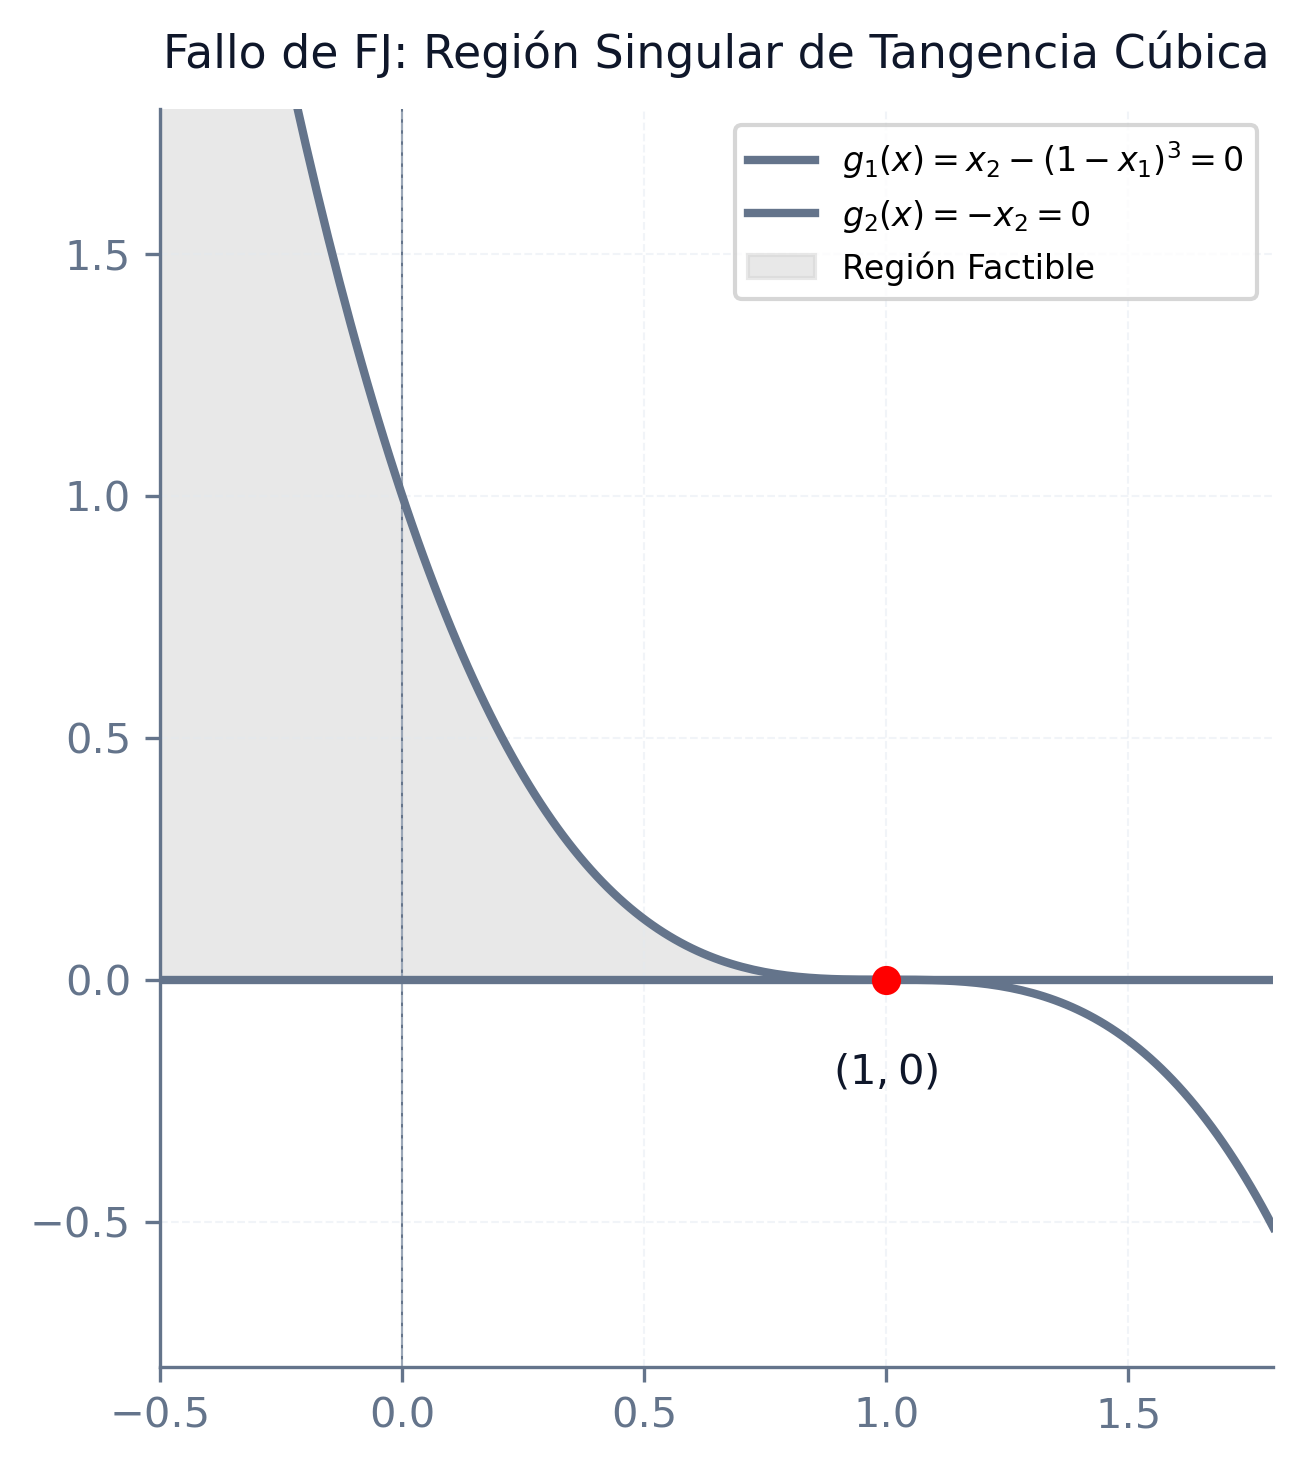
\includegraphics[width=0.6\linewidth,height=\textheight,keepaspectratio]{images/fj_ejemplo_cuba.png}

}

\caption{\label{fig-fj-ejemplo-cuba}Visualización de la región factible
y la tangencia cúbica en \(\bar{x} = (1,0)\)}

\end{figure}%

\end{tcolorbox}

Para apreciar la diferencia que introduce una formulación regular en la
frontera, consideremos ahora el mismo problema pero sustituyendo la
restricción cúbica singular por una restricción lineal equivalente. Al
regularizar la frontera, el punto singular desaparece, lo que permite
que el objetivo vuelva a participar activamente en la caracterización
del óptimo:

\begin{tcolorbox}[enhanced jigsaw, toprule=.15mm, opacitybacktitle=0.6, coltitle=black, colbacktitle=quarto-callout-tip-color!10!white, title=\textcolor{quarto-callout-tip-color}{\faLightbulb}\hspace{0.5em}{Ejemplo: Fritz-John regular con objetivo activo}, arc=.35mm, rightrule=.15mm, toptitle=1mm, breakable, bottomtitle=1mm, titlerule=0mm, colback=white, opacityback=0, leftrule=.75mm, colframe=quarto-callout-tip-color-frame, left=2mm, bottomrule=.15mm]

Si modificamos el problema anterior sustituyendo la restricción cúbica
por una restricción lineal regular: \[
\begin{aligned}
\min \quad & -x_1 \\
\text{s.a.} \quad & g_1(x_1, x_2) = x_1 + x_2 - 1 \le 0 \\
& g_2(x_1, x_2) = -x_2 \le 0
\end{aligned}
\] En el óptimo \(\bar{x} = (1, 0)\) (véase la
Figura~\ref{fig-fj-ejemplo-lineal}), ambas restricciones son activas. La
ecuación de Fritz-John es:
\[ u_0 \begin{pmatrix} -1 \\ 0 \end{pmatrix} + u_1 \begin{pmatrix} 1 \\ 1 \end{pmatrix} + u_2 \begin{pmatrix} 0 \\ -1 \end{pmatrix} = \begin{pmatrix} 0 \\ 0 \end{pmatrix} \implies \begin{aligned} -u_0 + u_1 &= 0 \\ u_1 - u_2 &= 0 \end{aligned} \]
Lo que nos da \(u_1 = u_2 = u_0\). Podemos fijar \(u_0 = 1\) para
obtener la solución regular \(u_1 = u_2 = 1 > 0\), donde la función
objetivo influye activamente en el óptimo.

\begin{figure}[H]

\centering{

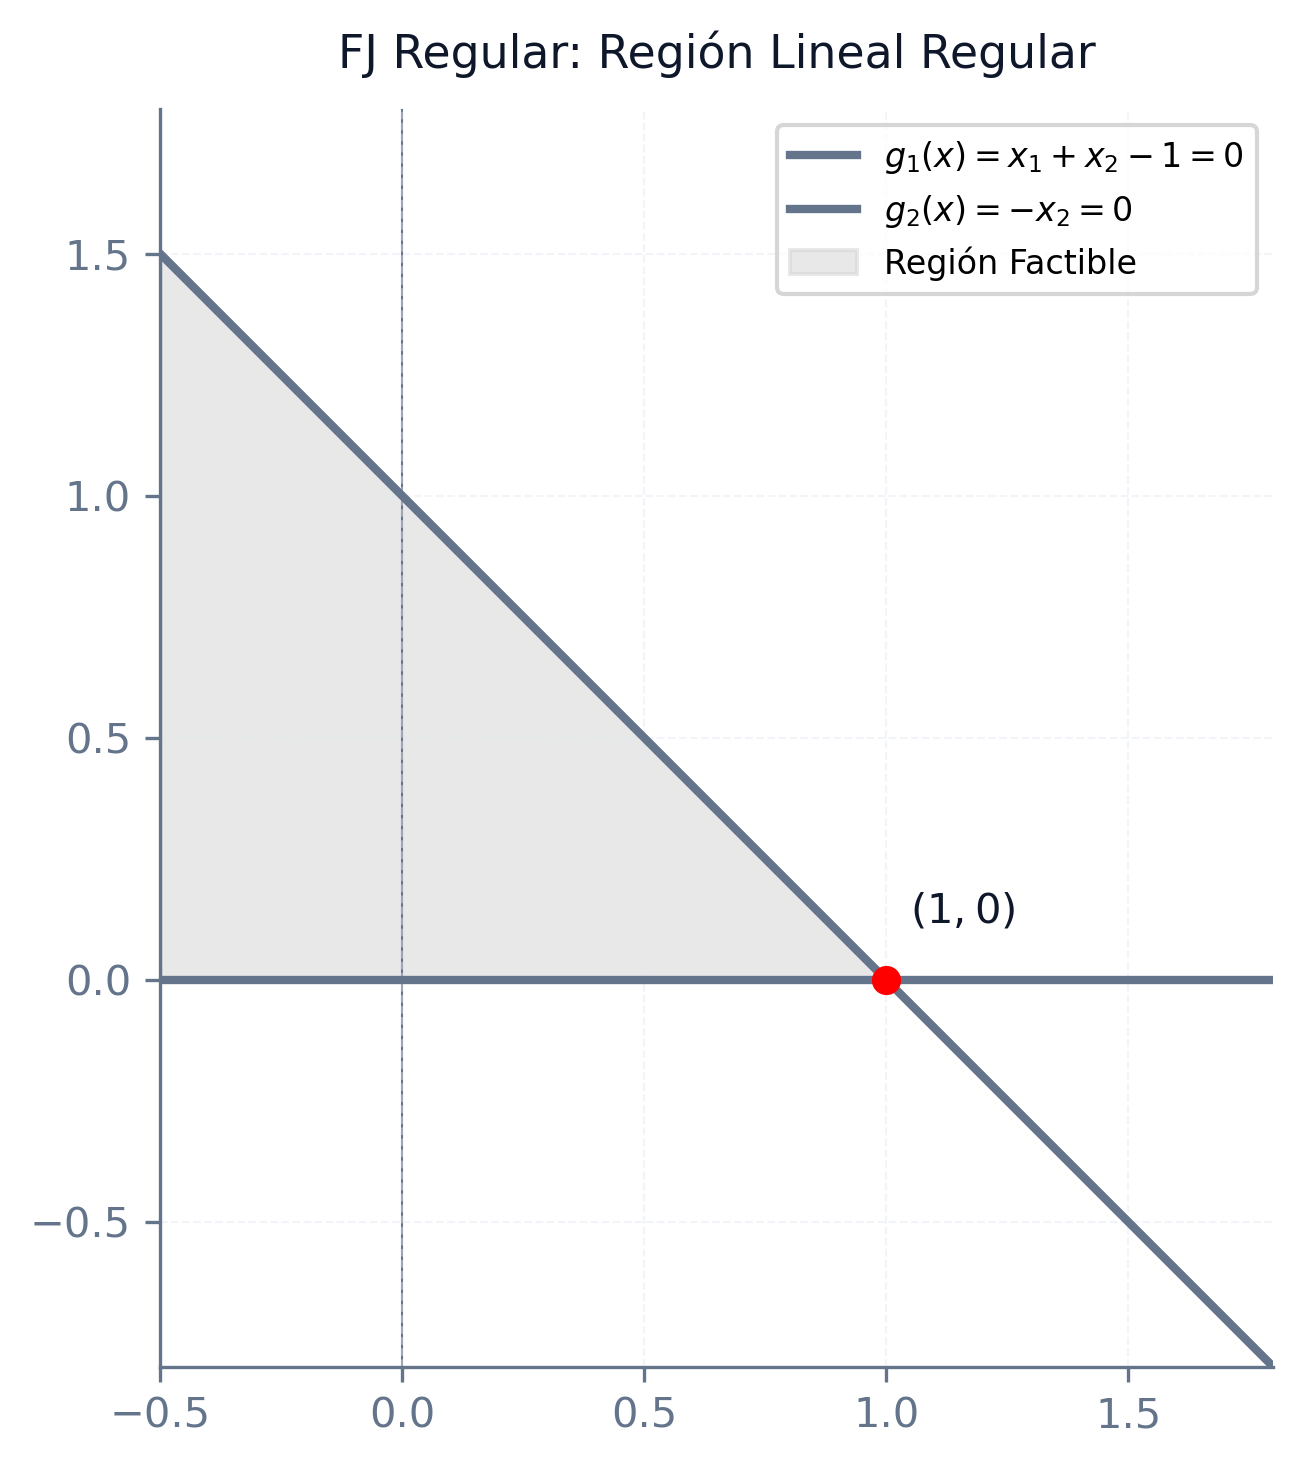
\includegraphics[width=0.6\linewidth,height=\textheight,keepaspectratio]{images/fj_ejemplo_lineal.png}

}

\caption{\label{fig-fj-ejemplo-lineal}Visualización de la región
factible regular y lineal en \(\bar{x} = (1, 0)\)}

\end{figure}%

\end{tcolorbox}

Los ejemplos anteriores muestran que existen puntos que verifican las
condiciones de Fritz-John de forma trivial, perdiendo toda la
sensibilidad respecto a la función objetivo. La teoría general
identifica tres escenarios habituales de esta vulnerabilidad dual:

\begin{enumerate}
\def\labelenumi{\arabic{enumi}.}
\tightlist
\item
  \textbf{Estacionariedad simultánea}: Si en el punto candidato
  coinciden un mínimo local libre del objetivo y un punto de tangencia
  de restricciones, de manera que \(\nabla f(\bar{x}) = 0\) y
  \(\nabla g_i(\bar{x}) = 0\) para algún \(i \in \mathcal{I}\), entonces
  es posible tomar \(u_0 > 0\) e \(u_i > 0\) con el resto de los
  multiplicadores nulos. Esto satisface las condiciones de Fritz-John de
  forma trivial sin reflejar la influencia real del acoplamiento de las
  restricciones.
\item
  \textbf{Desdoblamiento de restricciones de igualdad}: Si una
  restricción de igualdad \(h(x) = 0\) se sustituye por dos
  desigualdades \(h(x) \le 0\) y \(-h(x) \le 0\), en cualquier punto
  factible ambas restricciones son activas con gradientes opuestos
  \(\nabla h(\bar{x})\) y \(-\nabla h(\bar{x})\). Esto permite anular el
  sistema dual de Fritz-John de forma trivial asignando un valor
  positivo a los multiplicadores de estas restricciones y cero al resto,
  independientemente de la función objetivo (provocando \(u_0 = 0\)).
\item
  \textbf{Redundancia trivial en la frontera}: Como vimos en la
  advertencia teórica, siempre es posible añadir una restricción
  redundante del tipo \(\|x - \bar{x}\| \ge 0\), que es universalmente
  cierta. En el punto \(\bar{x}\), esta restricción se activa y su
  gradiente es nulo, lo que anula el cono de restricciones activas
  \(\mathcal{G}_0 = \emptyset\) y fuerza \(u_0 = 0\) en el sistema dual.
\end{enumerate}

\section{Condiciones de Karush-Kuhn-Tucker
(KKT)}\label{condiciones-de-karush-kuhn-tucker-kkt}

Existen problemas de optimización en los que se hallan puntos de
Fritz-John con multiplicador \(u_0 = 0\). Esto ocurre, por ejemplo,
cuando el cono de direcciones factibles es vacío
(\(\mathcal{G}_0 = \emptyset\)), ya que en tal escenario las condiciones
duales se verifican de manera trivial independientemente de la función
objetivo. En estas situaciones, el objetivo no interviene en la
caracterización del punto óptimo.

Para solventar esta anomalía y garantizar que la función objetivo
participe activamente en las condiciones de optimalidad
(\(u_0 \neq 0\)), William Karush en 1939 (en su tesis de maestría
inédita (Karush 1939)) e independientemente Harold W. Kuhn y Albert W.
Tucker en 1951 (Kuhn y Tucker 1951), desarrollaron condiciones que
imponen nuevas hipótesis de regularidad geométrica en las restricciones
del punto óptimo, denominadas \textbf{cualificaciones de restricciones}.

La cualificación de restricciones más habitual y de mayor relevancia
didáctica es la \textbf{Independencia Lineal de las Restricciones
Activas (LICQ)}, la cual exige que los gradientes de todas las
restricciones activas en el punto de estudio
\(\{\nabla g_i(\bar{x}), \forall i \in \mathcal{I}\}\) sean linealmente
independientes. Al añadir esta condición de regularidad, la ecuación de
Fritz-John obliga a que \(u_0 > 0\), lo que permite caracterizar el
óptimo con la participación directa de la función objetivo:

\begin{tcolorbox}[enhanced jigsaw, toprule=.15mm, opacitybacktitle=0.6, coltitle=black, colbacktitle=quarto-callout-important-color!10!white, title=\textcolor{quarto-callout-important-color}{\faExclamation}\hspace{0.5em}{Teorema: Condiciones necesarias de KKT}, arc=.35mm, rightrule=.15mm, toptitle=1mm, breakable, bottomtitle=1mm, titlerule=0mm, colback=white, opacityback=0, leftrule=.75mm, colframe=quarto-callout-important-color-frame, left=2mm, bottomrule=.15mm]

Sea el problema:
\[ \min \{f(x) \mid x \in \mathcal{X}, \ g_i(x) \le 0, \ i=1,\dots,m\} \]
y sea \(\bar{x}\) una solución factible, con el conjunto de
restricciones activas \(\mathcal{I} = \{i \mid g_i(\bar{x}) = 0\}\).
Supongamos que:

\begin{enumerate}
\def\labelenumi{\arabic{enumi}.}
\tightlist
\item
  Las funciones \(f\) y \(g_i\) (\(i \in \mathcal{I}\)) son
  diferenciables en \(\bar{x}\).
\item
  Las restricciones inactivas \(g_i\) (\(i \notin \mathcal{I}\)) son
  continuas en \(\bar{x}\).
\item
  Se verifica la cualificación de restricciones (LICQ) en \(\bar{x}\);
  es decir, los gradientes de las restricciones activas
  \(\{\nabla g_i(\bar{x}), i \in \mathcal{I}\}\) son linealmente
  independientes.
\end{enumerate}

Entonces, si \(\bar{x}\) es un mínimo local de \(f\), existen escalares
únicos \(\{u_i, i \in \mathcal{I}\}\), con \(u_i \ge 0\),
\(\forall i \in \mathcal{I}\) tales que:
\[ \nabla f(\bar{x}) + \sum_{i \in \mathcal{I}} u_i \nabla g_i(\bar{x}) = 0 \]

Si además se verifica que las restricciones inactivas
\(\{g_i, i \notin \mathcal{I}\}\) son también diferenciables en
\(\bar{x}\), las condiciones anteriores se extienden a todo el conjunto
de restricciones y se expresan de la forma estándar de KKT:

\begin{enumerate}
\def\labelenumi{\arabic{enumi}.}
\tightlist
\item
  \textbf{Factibilidad dual (Estacionariedad)}:
  \[ \nabla f(\bar{x}) + \sum_{i=1}^m u_i \nabla g_i(\bar{x}) = 0 \]
\item
  \textbf{Factibilidad primal}:
  \[ g_i(\bar{x}) \le 0, \quad \forall i = 1, \dots, m \]
\item
  \textbf{Holgura complementaria}:
  \[ u_i g_i(\bar{x}) = 0, \quad \forall i = 1, \dots, m \]
\item
  \textbf{No negatividad (Factibilidad dual de multiplicadores)}:
  \[ u_i \ge 0, \quad \forall i = 1, \dots, m \]
\end{enumerate}

Los escalares \(u_i\) reciben el nombre de \textbf{multiplicadores de
Lagrange}. Los puntos \(\bar{x}\) que satisfacen las condiciones KKT
anteriores (factibilidad primal, factibilidad dual y holgura
complementaria) se denominan \textbf{puntos KKT}.

\emph{Demostración}: Por las condiciones necesarias de Fritz-John,
existen multiplicadores no todos nulos \(u_0, \hat{u}_i \ge 0\) (para
\(i \in \mathcal{I}\)) tales que:
\[ u_0 \nabla f(\bar{x}) + \sum_{i \in \mathcal{I}} \hat{u}_i \nabla g_i(\bar{x}) = 0 \]
Probaremos por contradicción que \(u_0 > 0\). Si \(u_0 = 0\), la
ecuación se reduce a:
\[ \sum_{i \in \mathcal{I}} \hat{u}_i \nabla g_i(\bar{x}) = 0 \] Dado
que por la cualificación de restricciones (LICQ), los gradientes
\(\{\nabla g_i(\bar{x}), i \in \mathcal{I}\}\) son linealmente
independientes, la única combinación lineal que se anula es la trivial,
lo que exige que \(\hat{u}_i = 0\) para todo \(i \in \mathcal{I}\). Como
también habíamos supuesto \(u_0 = 0\), esto implica que todos los
multiplicadores son nulos, lo que contradice la condición de no
trivialidad de Fritz-John (\((u_0, \hat{u}) \neq 0\)).

Por tanto, se cumple que \(u_0 > 0\). Definiendo los multiplicadores
normalizados para las restricciones activas como
\(u_i = \frac{\hat{u}_i}{u_0} \ge 0\) (para \(i \in \mathcal{I}\)), se
obtiene la primera parte de la demostración. Tomando además \(u_j = 0\)
para las restricciones inactivas (\(j \notin \mathcal{I}\)), se obtiene
la segunda parte (formulación estándar de KKT). La unicidad de los
multiplicadores se deriva de la independencia lineal de los gradientes
de las restricciones activas. \(\blacksquare\)

\begin{figure}[H]

\centering{

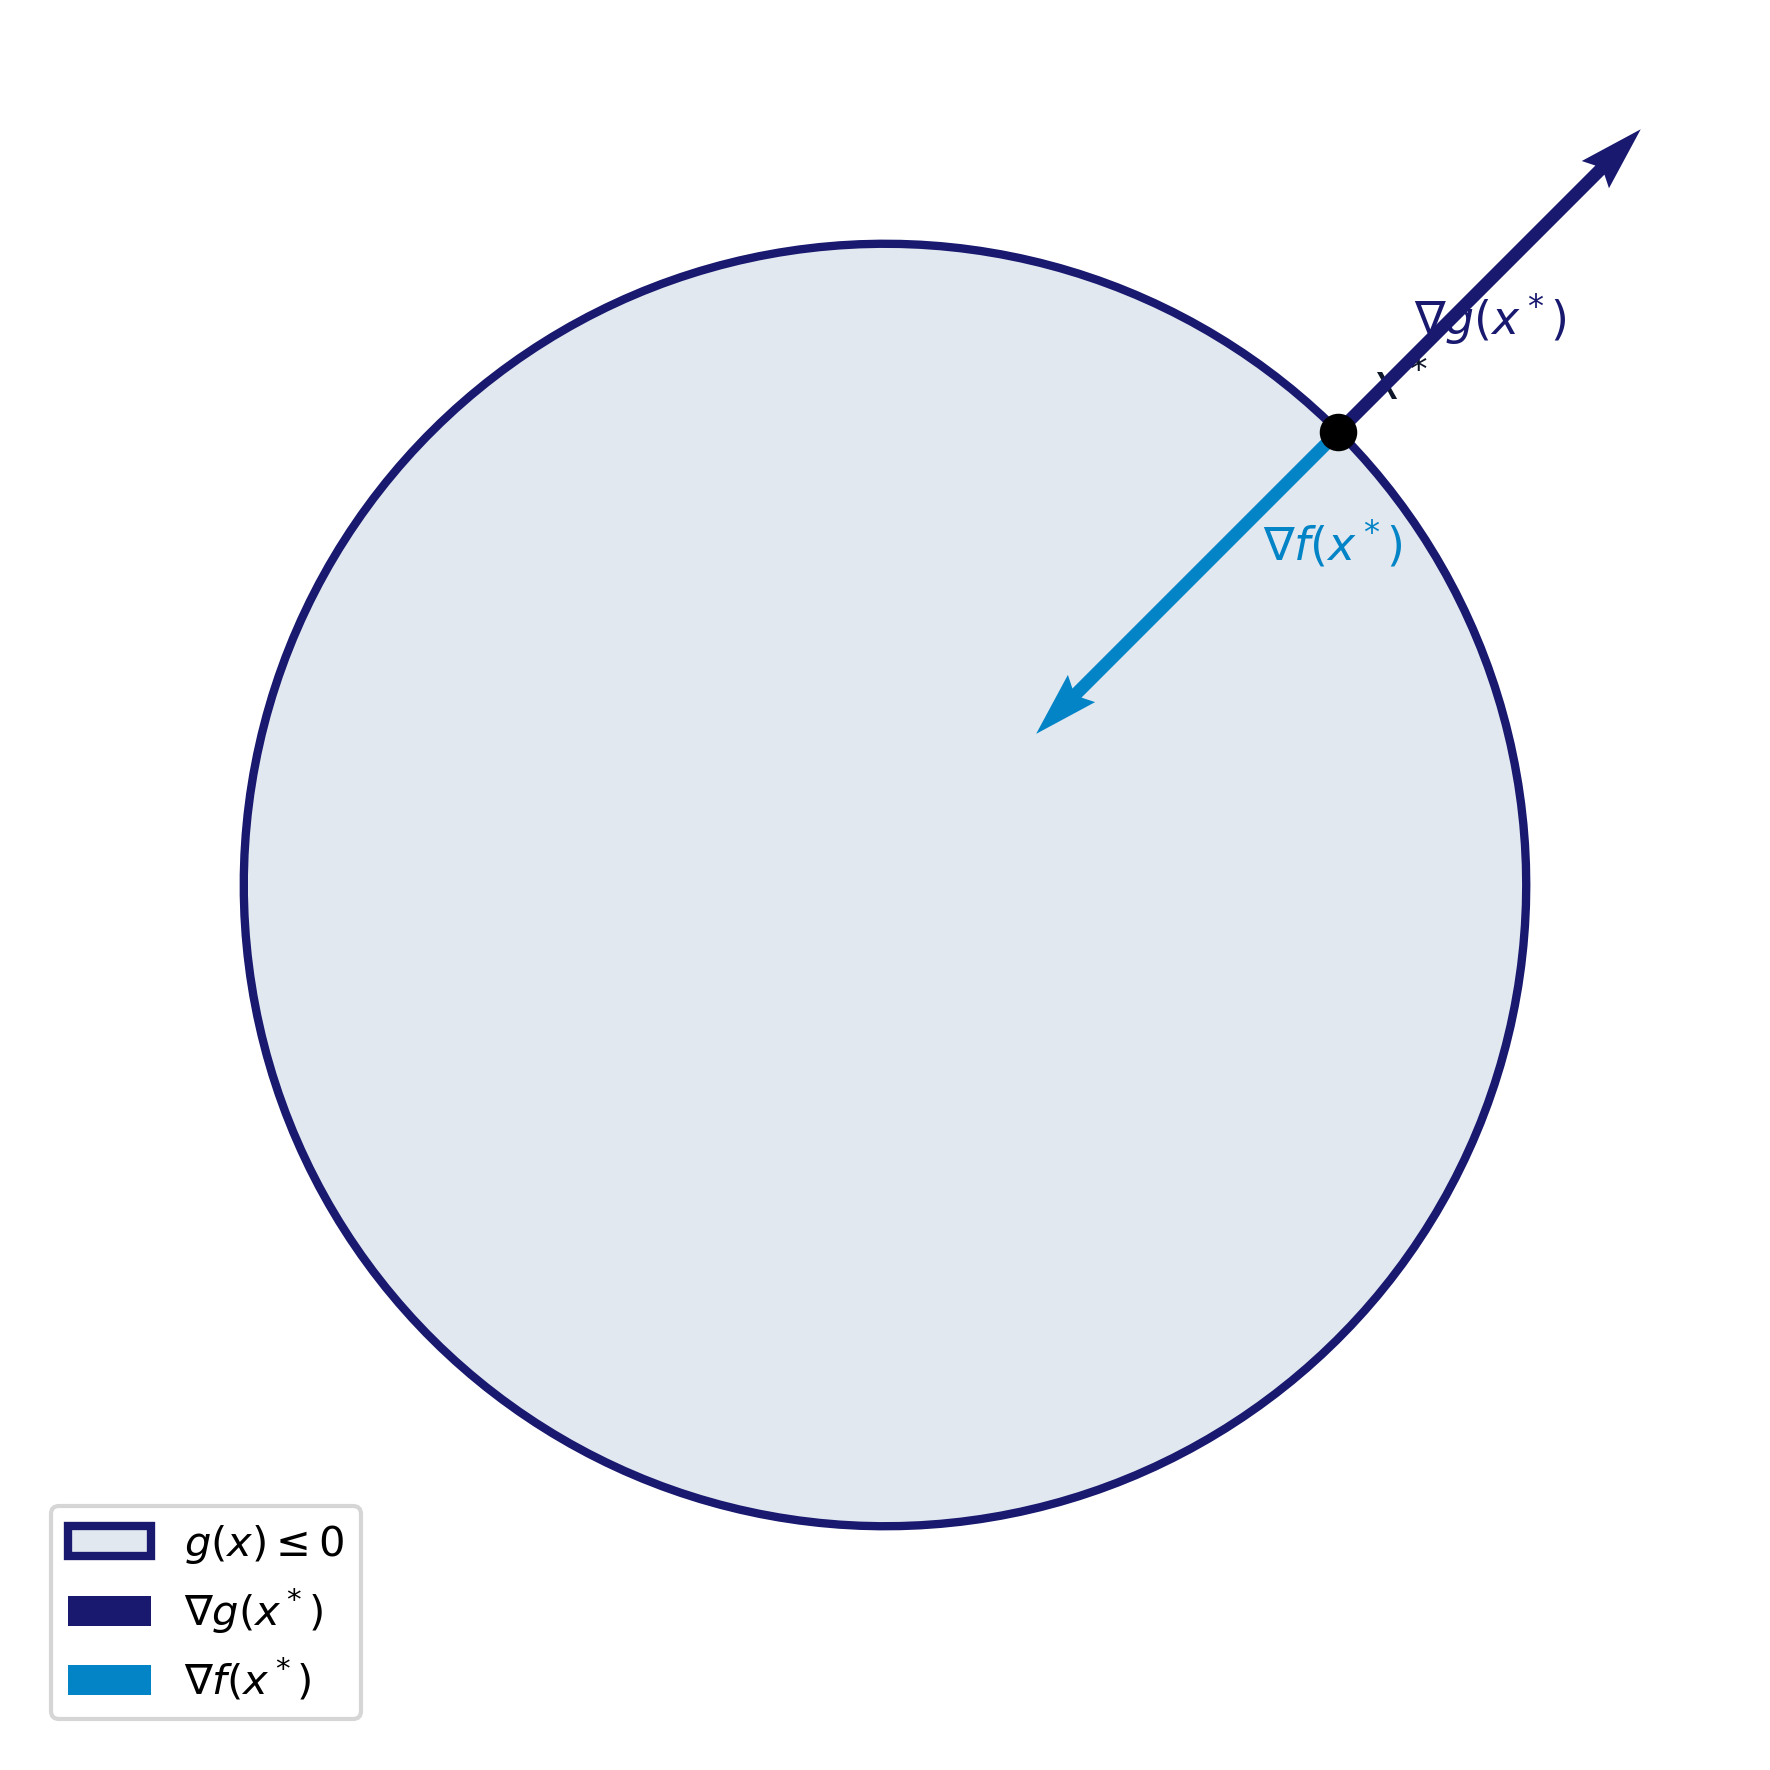
\includegraphics[width=0.6\linewidth,height=\textheight,keepaspectratio]{images/condiciones_kkt.png}

}

\caption{\label{fig-condiciones-kkt}Interpretación geométrica de las
condiciones KKT con restricciones activas}

\end{figure}%

\end{tcolorbox}

\begin{tcolorbox}[enhanced jigsaw, toprule=.15mm, opacitybacktitle=0.6, coltitle=black, colbacktitle=quarto-callout-warning-color!10!white, title=\textcolor{quarto-callout-warning-color}{\faExclamationTriangle}\hspace{0.5em}{Las condiciones KKT son únicamente necesarias}, arc=.35mm, rightrule=.15mm, toptitle=1mm, breakable, bottomtitle=1mm, titlerule=0mm, colback=white, opacityback=0, leftrule=.75mm, colframe=quarto-callout-warning-color-frame, left=2mm, bottomrule=.15mm]

Las condiciones KKT son únicamente \textbf{necesarias} en problemas
generales. Es fundamental señalar que no se aplican a todos los puntos,
sino que excluyen a aquellos que violan la cualificación de
restricciones (LICQ). Por consiguiente, existe la posibilidad de que el
óptimo global del problema se encuentre precisamente entre los puntos
excluidos (por ejemplo, en un punto singular de la frontera donde los
gradientes de las restricciones activas sean linealmente dependientes).
En cualquier resolución analítica, estos puntos singulares deben
analizarse de manera independiente.

Sin embargo, cabe destacar que para \textbf{problemas lineales}, las
condiciones KKT sí resultan ser necesarias y suficientes.

\end{tcolorbox}

\begin{tcolorbox}[enhanced jigsaw, toprule=.15mm, opacitybacktitle=0.6, coltitle=black, colbacktitle=quarto-callout-note-color!10!white, title=\textcolor{quarto-callout-note-color}{\faInfo}\hspace{0.5em}{Observación: Extensión a máximos locales}, arc=.35mm, rightrule=.15mm, toptitle=1mm, breakable, bottomtitle=1mm, titlerule=0mm, colback=white, opacityback=0, leftrule=.75mm, colframe=quarto-callout-note-color-frame, left=2mm, bottomrule=.15mm]

Si el punto \(\bar{x}\) es un máximo local, entonces las condiciones
necesarias de KKT siguen siendo válidas sin más que exigir que los
multiplicadores de Lagrange sean no positivos (\(u_i \le 0\),
\(\forall i = 1, \dots, m\)).

\end{tcolorbox}

Para dar el paso de condiciones necesarias a \textbf{suficientes} en
problemas generales no lineales y garantizar el carácter \textbf{global}
del mínimo, debemos exigir condiciones adicionales sobre la curvatura de
las funciones implicadas:

\begin{tcolorbox}[enhanced jigsaw, toprule=.15mm, opacitybacktitle=0.6, coltitle=black, colbacktitle=quarto-callout-important-color!10!white, title=\textcolor{quarto-callout-important-color}{\faExclamation}\hspace{0.5em}{Teorema: Condiciones suficientes de KKT bajo convexidad}, arc=.35mm, rightrule=.15mm, toptitle=1mm, breakable, bottomtitle=1mm, titlerule=0mm, colback=white, opacityback=0, leftrule=.75mm, colframe=quarto-callout-important-color-frame, left=2mm, bottomrule=.15mm]

Sea \(\bar{x}\) un punto factible que satisface las condiciones
necesarias de KKT con multiplicadores \(u_i\). Si:

\begin{enumerate}
\def\labelenumi{\arabic{enumi}.}
\tightlist
\item
  La función objetivo \(f(x)\) es \textbf{pseudo-convexa} en
  \(\bar{x}\).
\item
  Las restricciones activas \(g_i(x)\) (\(i \in \mathcal{I}\)) son
  \textbf{cuasi-convexas} y diferenciables en \(\bar{x}\).
\end{enumerate}

Entonces \(\bar{x}\) es un mínimo global del problema.

\emph{Demostración}: Sea \(x\) un punto factible cualquiera del
problema, lo que implica que \(g_i(x) \le 0\) para todo
\(i = 1, \dots, m\). Para las restricciones activas
(\(i \in \mathcal{I}\)), se cumple que \(g_i(\bar{x}) = 0\), lo que nos
da: \[ g_i(x) \le g_i(\bar{x}) = 0, \quad \forall i \in \mathcal{I} \]
Puesto que las restricciones activas \(g_i\) (\(i \in \mathcal{I}\)) son
cuasi-convexas y diferenciables en \(\bar{x}\), por la definición de
cuasi-convexidad se tiene que para cualquier \(\lambda \in [0, 1]\):
\[ g_i(\bar{x} + \lambda(x - \bar{x})) \le \max\{g_i(x), g_i(\bar{x})\} \le g_i(\bar{x}) = 0 \]
Esto implica que la función \(g_i\) no crece cuando nos desplazamos
desde el punto óptimo \(\bar{x}\) en la dirección de factibilidad
\((x - \bar{x})\). Por lo tanto, \((x - \bar{x})\) es una dirección de
no ascenso (o dirección de descenso) en \(\bar{x}\), lo que se traduce
en:
\[ \nabla g_i(\bar{x})^T (x - \bar{x}) \le 0, \quad \forall i \in \mathcal{I} \]
Como los multiplicadores KKT son no negativos (\(u_i \ge 0\)), al
multiplicar cada una de estas expresiones y sumarlas sobre el conjunto
de restricciones activas \(\mathcal{I}\), obtenemos:
\[ \sum_{i \in \mathcal{I}} u_i \nabla g_i(\bar{x})^T (x - \bar{x}) \le 0 \]
Por la condición de estacionariedad (factibilidad dual) de KKT, se tiene
que
\(\sum_{i \in \mathcal{I}} u_i \nabla g_i(\bar{x}) = -\nabla f(\bar{x})\).
Sustituyendo esta igualdad en la desigualdad anterior:
\[ \nabla f(\bar{x})^T (x - \bar{x}) = -\sum_{i \in \mathcal{I}} u_i \nabla g_i(\bar{x})^T (x - \bar{x}) \ge 0 \]
Finalmente, puesto que la función objetivo \(f\) es pseudo-convexa en
\(\bar{x}\), la condición de primer orden
\(\nabla f(\bar{x})^T (x - \bar{x}) \ge 0\) garantiza que:
\[ f(x) \ge f(\bar{x}) \] Como esta desigualdad es válida para todo
punto factible \(x\), concluimos que \(\bar{x}\) es un mínimo global del
problema. \blacksquare

\end{tcolorbox}

\begin{tcolorbox}[enhanced jigsaw, toprule=.15mm, opacitybacktitle=0.6, coltitle=black, colbacktitle=quarto-callout-note-color!10!white, title=\textcolor{quarto-callout-note-color}{\faInfo}\hspace{0.5em}{Observación sobre suficiencia local y unicidad}, arc=.35mm, rightrule=.15mm, toptitle=1mm, breakable, bottomtitle=1mm, titlerule=0mm, colback=white, opacityback=0, leftrule=.75mm, colframe=quarto-callout-note-color-frame, left=2mm, bottomrule=.15mm]

\begin{itemize}
\tightlist
\item
  Si las condiciones de pseudo-convexidad, cuasi-convexidad y
  diferenciabilidad se verifican sólo localmente en un entorno de
  \(\bar{x}\), entonces \(\bar{x}\) será un mínimo local.
\item
  Si el punto \(\bar{x}\) es un máximo local, entonces, para que sea
  máximo global en la primera condición hay que exigir que la función
  objetivo \(f\) sea \textbf{pseudo-cóncava} (o equivalentemente, \(-f\)
  sea pseudo-convexa).
\item
  Asimismo, si la función objetivo es estrictamente pseudo-convexa, el
  punto mínimo global \(\bar{x}\) es único.
\end{itemize}

\end{tcolorbox}

\begin{tcolorbox}[enhanced jigsaw, toprule=.15mm, opacitybacktitle=0.6, coltitle=black, colbacktitle=quarto-callout-tip-color!10!white, title=\textcolor{quarto-callout-tip-color}{\faLightbulb}\hspace{0.5em}{Ejemplo: Análisis por casos de KKT}, arc=.35mm, rightrule=.15mm, toptitle=1mm, breakable, bottomtitle=1mm, titlerule=0mm, colback=white, opacityback=0, leftrule=.75mm, colframe=quarto-callout-tip-color-frame, left=2mm, bottomrule=.15mm]

Consideremos el problema de encontrar los candidatos a mínimos y máximos
locales y globales de: \[
\begin{aligned}
\min/\max \quad & f(x_1, x_2) = x_1 + x_2 \\
\text{s.a.} \quad & g_1(x_1, x_2) = x_1^2 + x_2^2 - 4 \le 0 \\
& g_2(x_1, x_2) = -x_1^2 + x_2 \le 0
\end{aligned}
\]

Calculamos en primer lugar los gradientes de las funciones implicadas:
\[
\nabla f(x) = \begin{pmatrix} 1 \\ 1 \end{pmatrix}, \quad \nabla g_1(x) = \begin{pmatrix} 2x_1 \\ 2x_2 \end{pmatrix}, \quad \nabla g_2(x) = \begin{pmatrix} -2x_1 \\ 1 \end{pmatrix}
\]

La función Lagrangiana del problema es:
\[ L(x_1, x_2, u_1, u_2) = x_1 + x_2 + u_1(x_1^2 + x_2^2 - 4) + u_2(-x_1^2 + x_2) \]

El sistema de condiciones KKT (que integra estacionariedad, factibilidad
primal, ortogonalidad y no negatividad) se plantea como:

\begin{enumerate}
\def\labelenumi{\arabic{enumi}.}
\item
  \textbf{Estacionariedad (Factibilidad dual)}:
  \[ \frac{\partial L}{\partial x_1} = 1 + 2u_1 x_1 - 2u_2 x_1 = 0 \implies 1 + 2x_1(u_1 - u_2) = 0 \]
  \[ \frac{\partial L}{\partial x_2} = 1 + 2u_1 x_2 + u_2 = 0 \]
\item
  \textbf{Factibilidad primal}: \[ x_1^2 + x_2^2 - 4 \le 0 \]
  \[ -x_1^2 + x_2 \le 0 \]
\item
  \textbf{Ortogonalidad (Holgura complementaria)}:
  \[ u_1(x_1^2 + x_2^2 - 4) = 0 \] \[ u_2(-x_1^2 + x_2) = 0 \]
\item
  \textbf{No negatividad / No positividad}:

  \begin{itemize}
  \tightlist
  \item
    Para \textbf{mínimos}: \(u_1, u_2 \ge 0\).
  \item
    Para \textbf{máximos}: \(u_1, u_2 \le 0\).
  \end{itemize}
\end{enumerate}

En la Figura~\ref{fig-kkt-ejemplo-circ-parab-general} se representa la
geometría general del problema. La región factible \(\mathcal{S}\) está
sombreada en gris (delimitada por la circunferencia en azul oscuro y la
parábola en rojo brick), y las líneas discontinuas paralelas representan
las curvas de nivel del objetivo \(f(x_1, x_2) = x_1 + x_2\), cuyo
gradiente \(\nabla f\) apunta a 45 grados en dirección noreste.

\begin{figure}[H]

\centering{

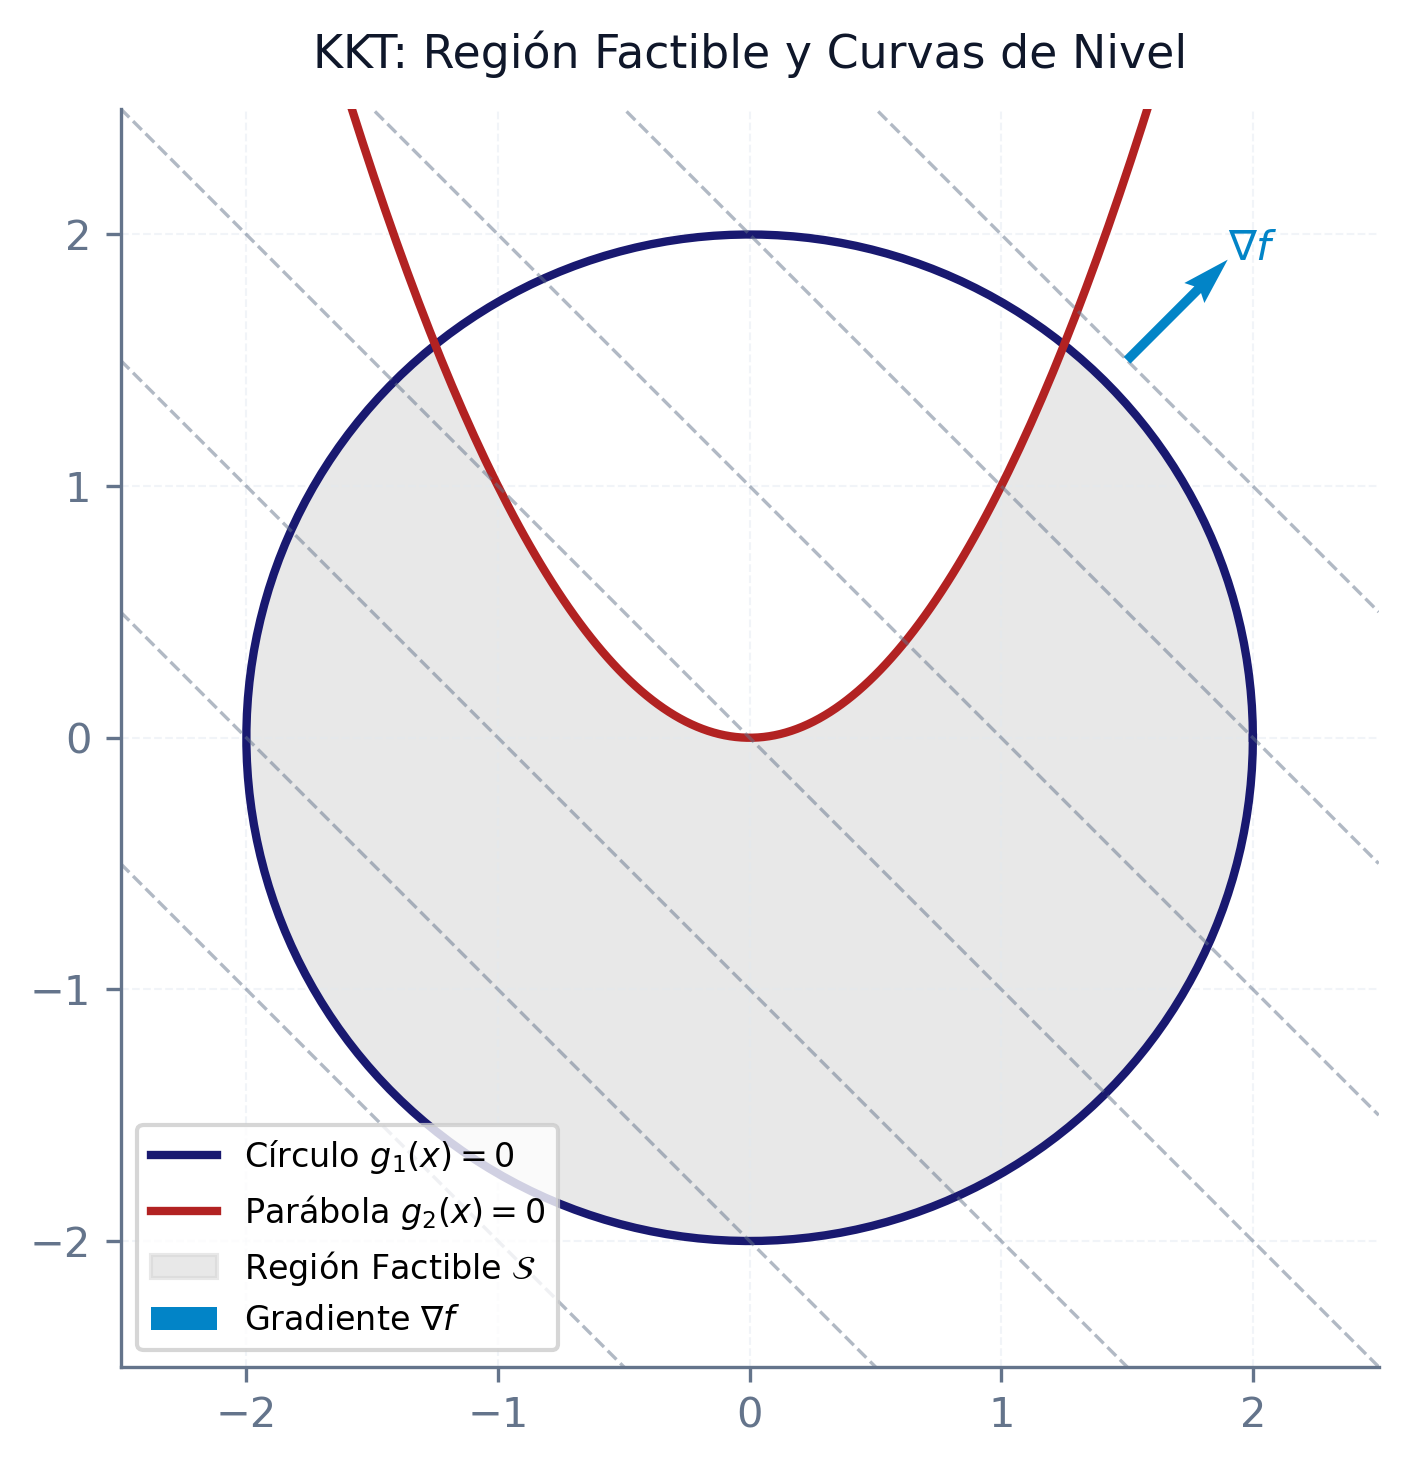
\includegraphics[width=0.6\linewidth,height=\textheight,keepaspectratio]{images/kkt_ejemplo_circ_parab.png}

}

\caption{\label{fig-kkt-ejemplo-circ-parab-general}KKT: Región Factible
y Curvas de Nivel}

\end{figure}%

Observamos que no es posible que ambas restricciones sean inactivas
(\(u_1 = 0, u_2 = 0\)), ya que en tal caso la condición de
estacionariedad exigiría \(\nabla f(x) = (1,1)^T = (0,0)^T\), lo cual es
imposible. Por tanto, procedemos a analizar los casos restantes:

Analizamos a continuación la resolución por casos combinatorios de
restricciones activas para desgranar paso a paso el problema:

\textbf{Caso 1: Círculo inactivo (\(u_1 = 0 \implies u_2 \neq 0\))} El
sistema de estacionariedad se reduce a:
\[ 1 - 2u_2 x_1 = 0 \quad \text{y} \quad 1 + u_2 = 0 \implies u_2 = -1 \]
Con \(u_2 = -1\), sustituimos en la primera ecuación:
\(1 - 2(-1)x_1 = 0 \implies x_1 = -1/2\). Dado que \(u_2 = -1 \neq 0\),
la holgura complementaria exige que la restricción \(g_2\) sea activa
(\(g_2(x) = 0\)), lo que nos da \(x_2 = x_1^2 = (-1/2)^2 = 1/4\). Esto
nos da el punto candidato \(A = (-1/2, 1/4)\).

\begin{itemize}
\tightlist
\item
  \textbf{Análisis del signo del multiplicador}: Obtenemos \(u_2 = -1\).

  \begin{itemize}
  \tightlist
  \item
    Para \textbf{mínimos}, requerimos \(u_i \ge 0\), por lo que \(A\)
    queda descartado.
  \item
    Para \textbf{máximos}, requerimos \(u_i \le 0\). Dado que
    \(u_2 = -1 \le 0\), el punto \(A = (-1/2, 1/4)\) es un candidato de
    primer orden a máximo local. Sin embargo, al realizar un análisis de
    segundo orden a lo largo de la frontera parabólica activa
    \(g_2(x) = 0\), observamos que la función restringida a esta
    frontera es \(f(t, t^2) = t + t^2\), la cual presenta un mínimo
    local en \(t = -0.5\) (con \(f(A) = -0.25\)). Esto implica que en
    cualquier entorno de \(A\) existen puntos factibles en la frontera
    parabólica con valores mayores que \(f(A)\) (por ejemplo, para
    \(t = -0.5 + \epsilon\)). Por lo tanto, el punto \(A\) \textbf{no es
    un máximo local} (ni tampoco un mínimo), siendo un punto que no es
    ni máximo ni mínimo o ``ni máx ni mín''.
  \end{itemize}
\item
  \textbf{Comprobación de factibilidad primal}: Verificamos si \(A\)
  cumple la restricción inactiva \(g_1\):
  \[ g_1(-1/2, 1/4) = (-1/2)^2 + (1/4)^2 - 4 = 1/4 + 1/16 - 4 = -59/16 < 0 \quad (\text{factible}) \]
\end{itemize}

Geométricamente (ver Figura~\ref{fig-kkt-ejemplo-circ-parab-caso-a}), en
el punto \(A(-1/2, 1/4)\) el gradiente de la función objetivo
\(\nabla f(A) = (1,1)^T\) apunta en la misma dirección que la normal de
la restricción activa \(\nabla g_2(A) = (1,1)^T\). Al apuntar en el
mismo sentido, se cumple la condición necesaria de primer orden de KKT
para máximo. Sin embargo, dado que la frontera de la restricción es
convexa (la parábola se curva ``alejándose'' de las curvas de nivel
superiores), al movernos a lo largo de ella la función \(f\) comienza a
crecer, impidiendo que \(A\) sea un máximo local. El gráfico de detalle
con las curvas de nivel en gradiente ilustra esta tangencia crítica (ver
Figura~\ref{fig-kkt-ejemplo-circ-parab-caso-a-general} y
Figura~\ref{fig-kkt-ejemplo-circ-parab-caso-a-detalle}).

\begin{figure}[H]

\begin{minipage}{0.50\linewidth}

\centering{

\pandocbounded{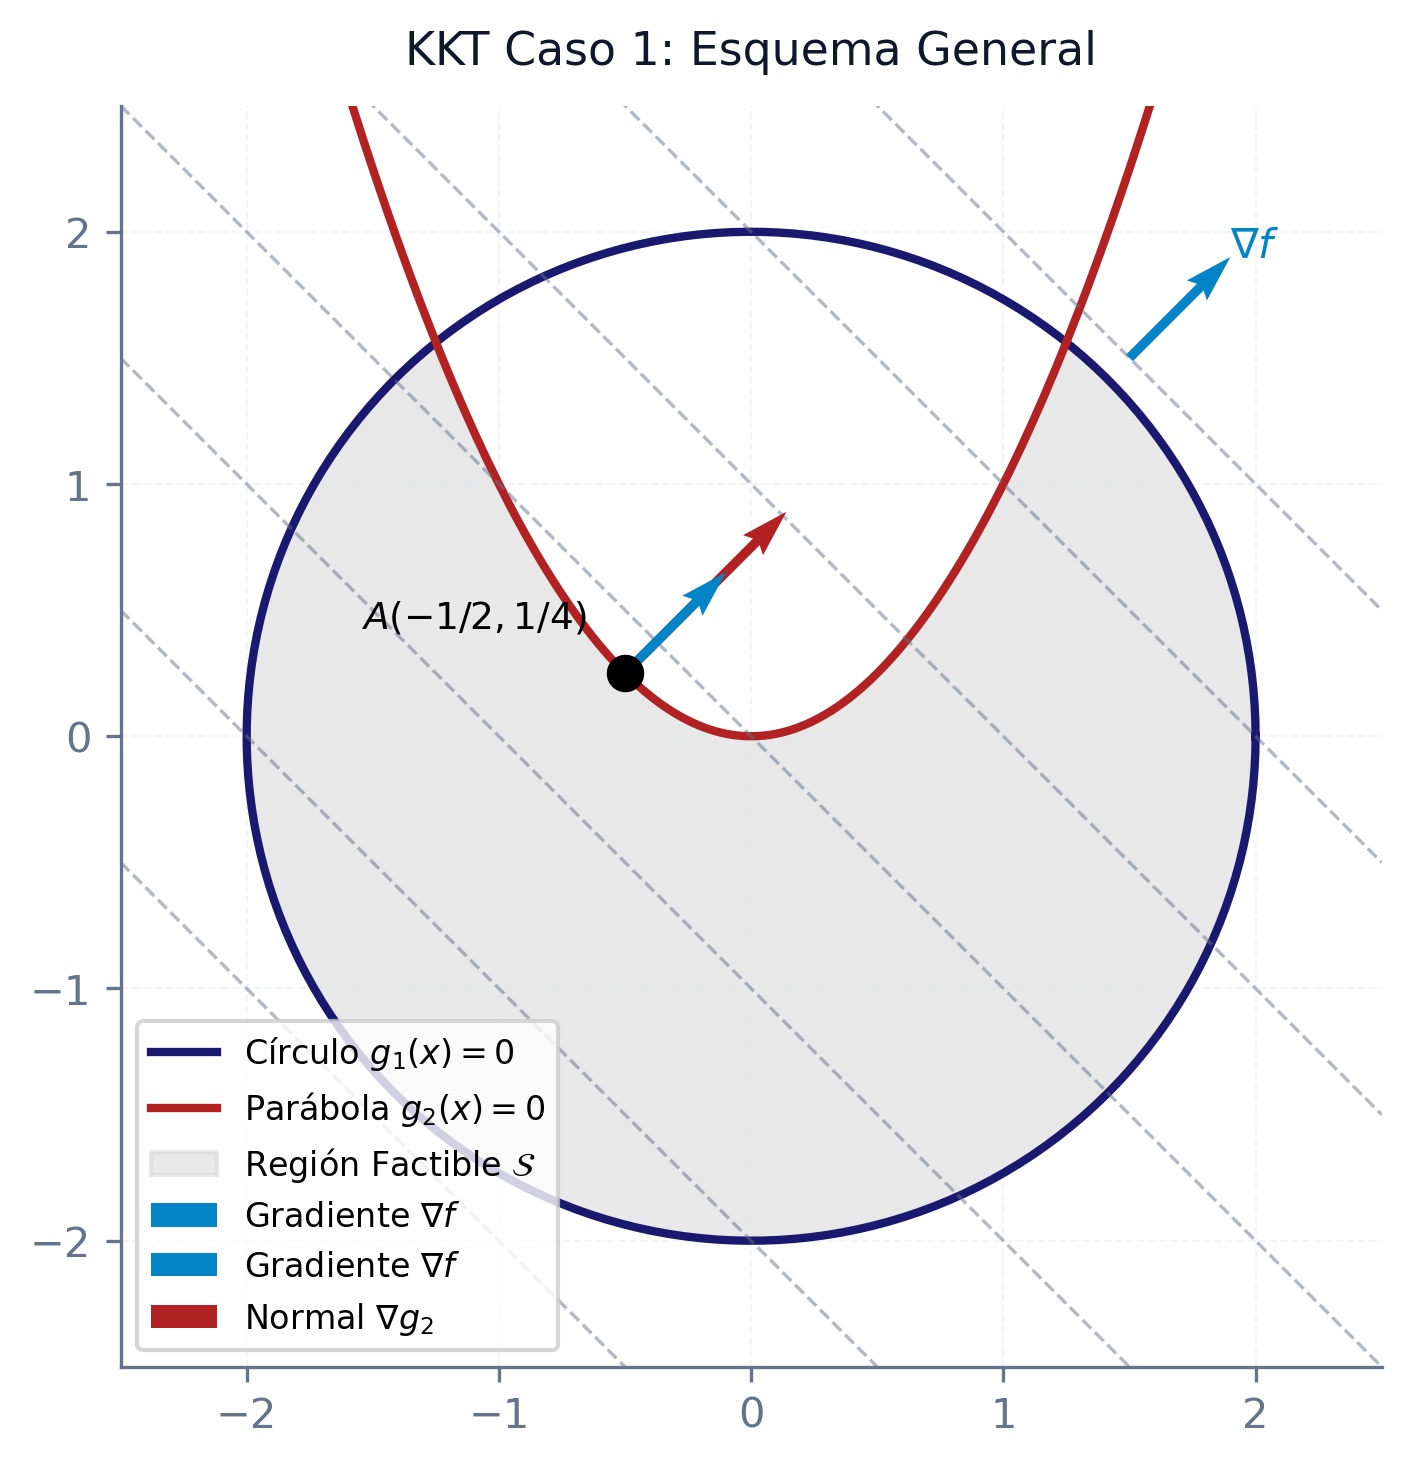
\includegraphics[keepaspectratio]{images/kkt_ejemplo_circ_parab_caso_a_general.png}}

}

\subcaption{\label{fig-kkt-ejemplo-circ-parab-caso-a-general}Esquema
general}

\end{minipage}%
%
\begin{minipage}{0.50\linewidth}

\centering{

\pandocbounded{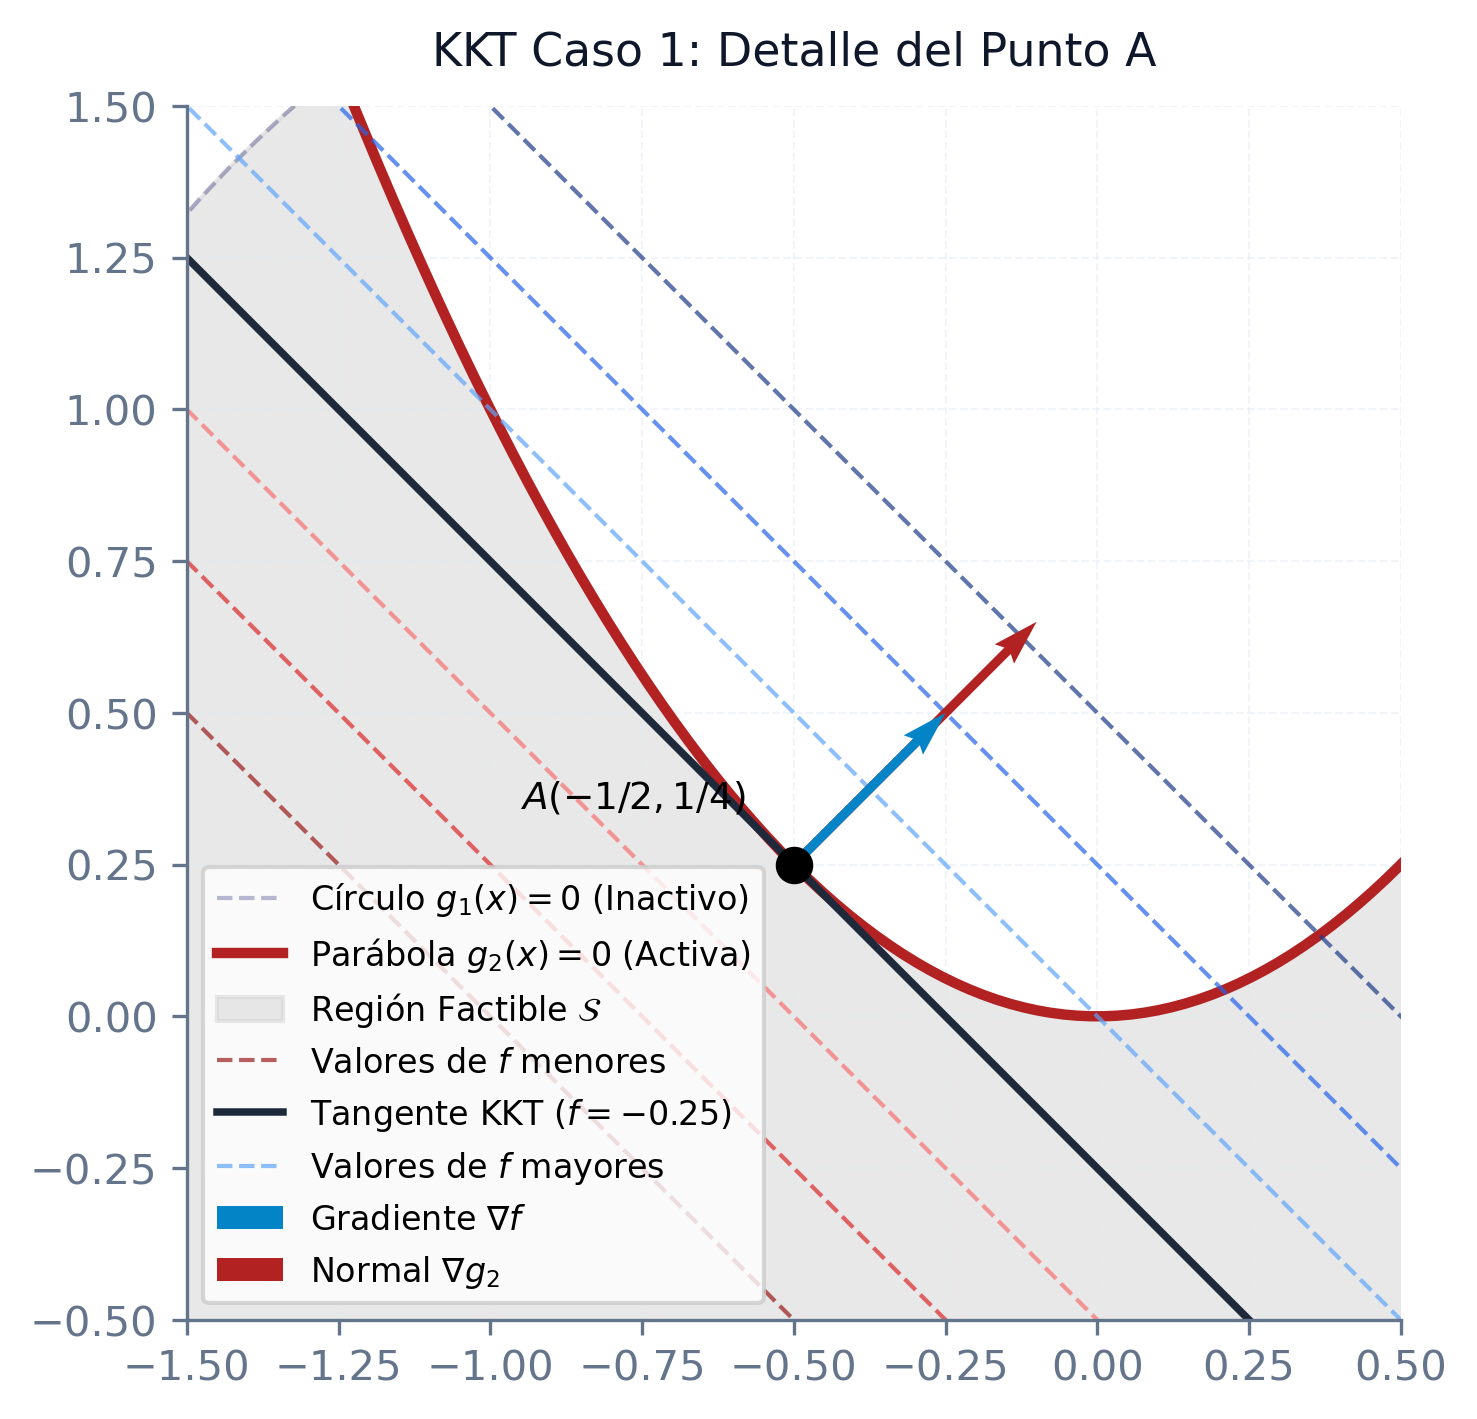
\includegraphics[keepaspectratio]{images/kkt_ejemplo_circ_parab_caso_a.png}}

}

\subcaption{\label{fig-kkt-ejemplo-circ-parab-caso-a-detalle}Detalle del
punto \(A\) con gradiente de nivel}

\end{minipage}%

\caption{\label{fig-kkt-ejemplo-circ-parab-caso-a}Caso 1: Alineación de
gradientes con círculo inactivo y parábola activa}

\end{figure}%

\begin{center}\rule{0.5\linewidth}{0.5pt}\end{center}

\textbf{Caso 2: Parábola inactiva (\(u_2 = 0 \implies u_1 \neq 0\))} El
sistema se simplifica a:
\[ 1 + 2u_1 x_1 = 0 \quad \text{y} \quad 1 + 2u_1 x_2 = 0 \implies x_1 = x_2 = -\frac{1}{2u_1} \]
Como \(u_1 \neq 0\), la holgura complementaria exige que la restricción
\(g_1\) sea activa (\(g_1(x) = 0\)):
\[ x_1^2 + x_2^2 = 4 \implies 2x_1^2 = 4 \implies x_1^2 = 2 \implies x_1 = \pm\sqrt{2} \]
Esto nos proporciona dos puntos de estudio:

\begin{enumerate}
\def\labelenumi{\arabic{enumi}.}
\tightlist
\item
  \textbf{Punto \(B(-\sqrt{2}, -\sqrt{2})\)}: Sustituyendo
  \(x_1 = -\sqrt{2}\) obtenemos \(u_1 = \frac{1}{2\sqrt{2}} > 0\).

  \begin{itemize}
  \tightlist
  \item
    Dado que \(u_1 > 0\), es un \textbf{candidato a mínimo}.
  \item
    Comprobamos factibilidad primal en \(g_2\):
    \[g_2(-\sqrt{2}, -\sqrt{2}) = -(-\sqrt{2})^2 - \sqrt{2} = -2 - \sqrt{2} < 0\]
    (factible).
  \item
    Por tanto, el punto \(B(-\sqrt{2}, -\sqrt{2})\) es un
    \textbf{candidato KKT a mínimo global}.
  \end{itemize}
\item
  \textbf{Punto \(C(\sqrt{2}, \sqrt{2})\)}: Sustituyendo
  \(x_1 = \sqrt{2}\) obtenemos \(u_1 = -\frac{1}{2\sqrt{2}} < 0\).

  \begin{itemize}
  \tightlist
  \item
    Dado que \(u_1 < 0\), es un \textbf{candidato a máximo}.
  \item
    Comprobamos factibilidad primal en \(g_2\):
    \[g_2(\\sqrt{2}, \\sqrt{2}) = -(\\sqrt{2})^2 + \\sqrt{2} = -2 + \\sqrt{2} \\approx -0.59 < 0\]
    (factible).
  \item
    Por tanto, el punto \(C(\sqrt{2}, \sqrt{2})\) es un
    \textbf{candidato KKT a máximo global}.
  \end{itemize}
\end{enumerate}

Geométricamente (ver Figura~\ref{fig-kkt-ejemplo-circ-parab-caso-b}), en
\(B(-\sqrt{2}, -\sqrt{2})\) el gradiente del objetivo
\(\nabla f(B) = (1,1)^T\) apunta en dirección opuesta al vector normal
exterior del círculo \(\nabla g_1(B) = (-2\sqrt{2}, -2\sqrt{2})^T\), por
lo que se compensan con un multiplicador positivo \(u_1 > 0\), lo que
caracteriza a \(B\) como un mínimo (ver
Figura~\ref{fig-kkt-ejemplo-circ-parab-caso-b-detalle-b}). En cambio, en
\(C(\sqrt{2}, \sqrt{2})\) el gradiente del objetivo \(\nabla f(C)\)
apunta en el mismo sentido que la normal del círculo
\(\nabla g_1(C) = (2\sqrt{2}, 2\sqrt{2})^T\), cancelándose con un
multiplicador negativo \(u_1 < 0\), lo que caracteriza a \(C\) como un
máximo (ver Figura~\ref{fig-kkt-ejemplo-circ-parab-caso-b-detalle-c}).

\begin{figure}[H]

\begin{minipage}{0.33\linewidth}

\centering{

\pandocbounded{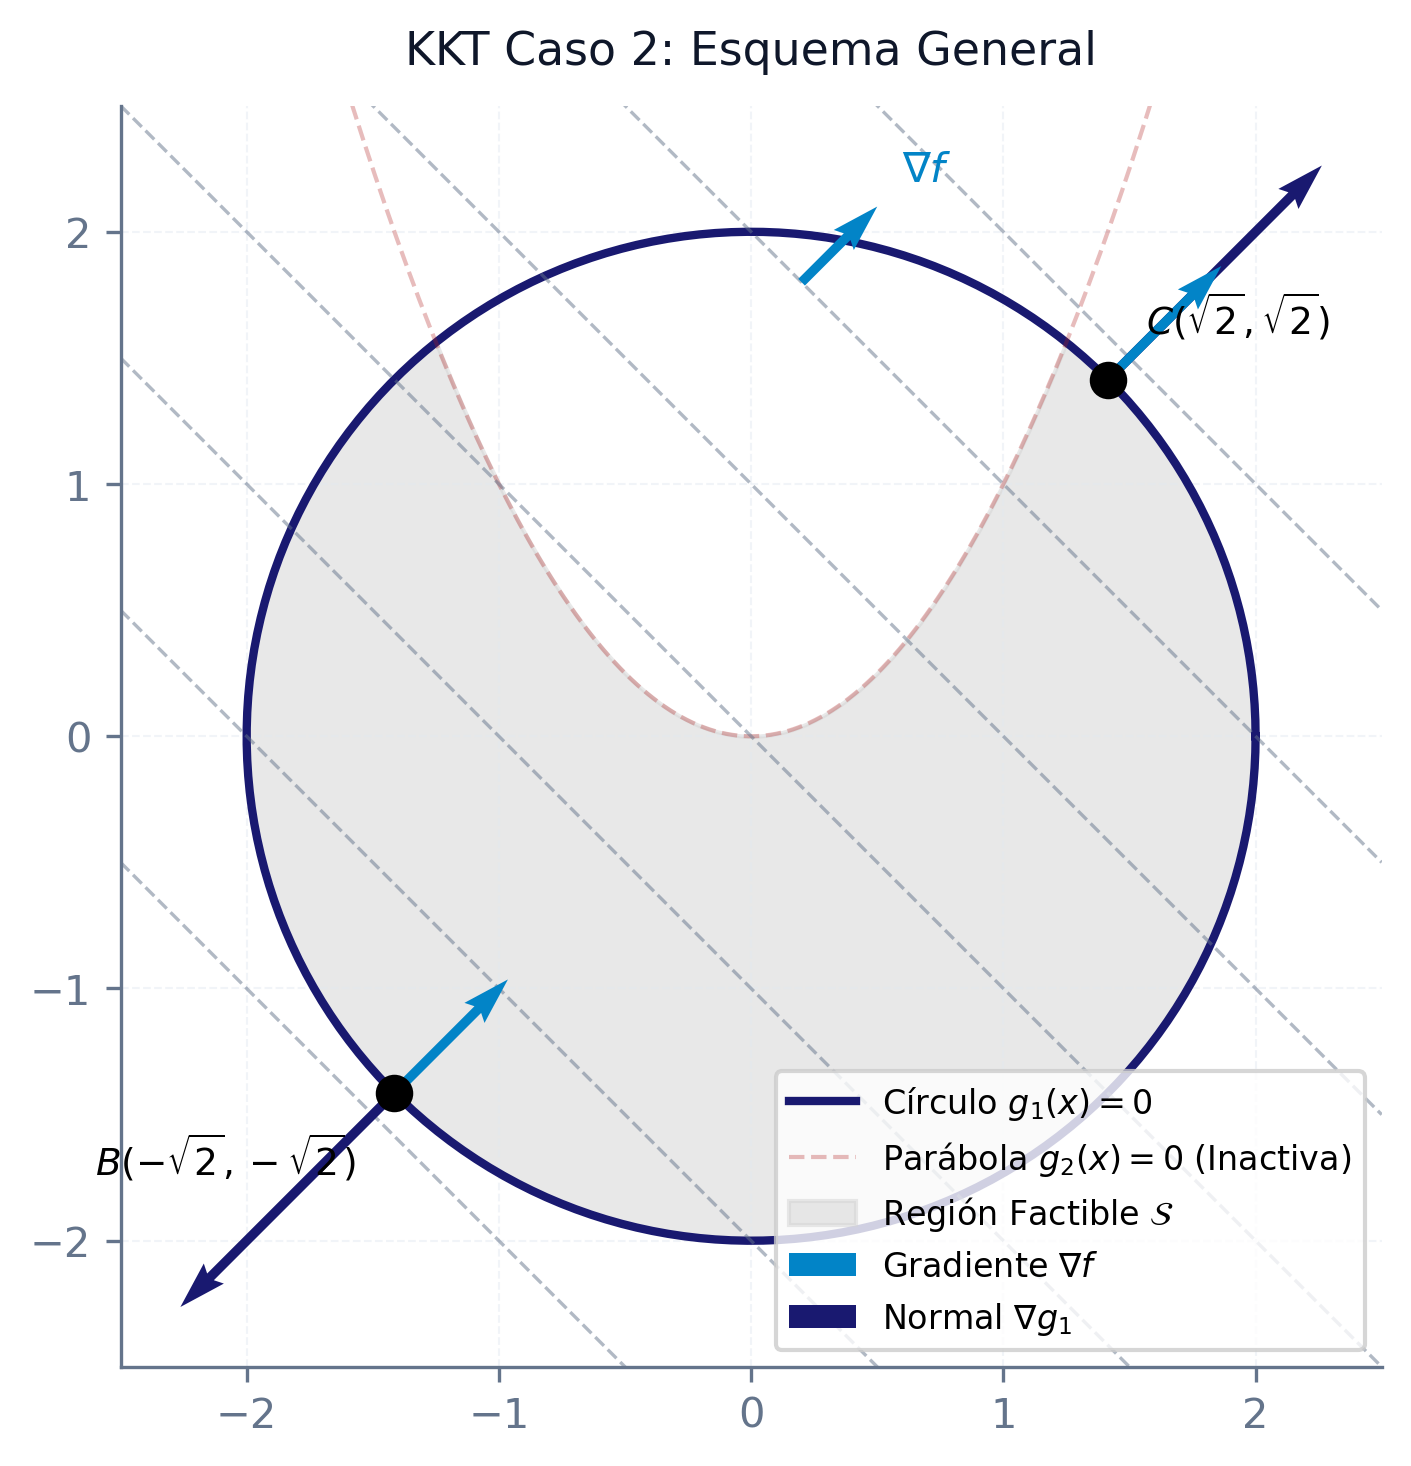
\includegraphics[keepaspectratio]{images/kkt_ejemplo_circ_parab_caso_b_general.png}}

}

\subcaption{\label{fig-kkt-ejemplo-circ-parab-caso-b-general}Esquema
general}

\end{minipage}%
%
\begin{minipage}{0.33\linewidth}

\centering{

\pandocbounded{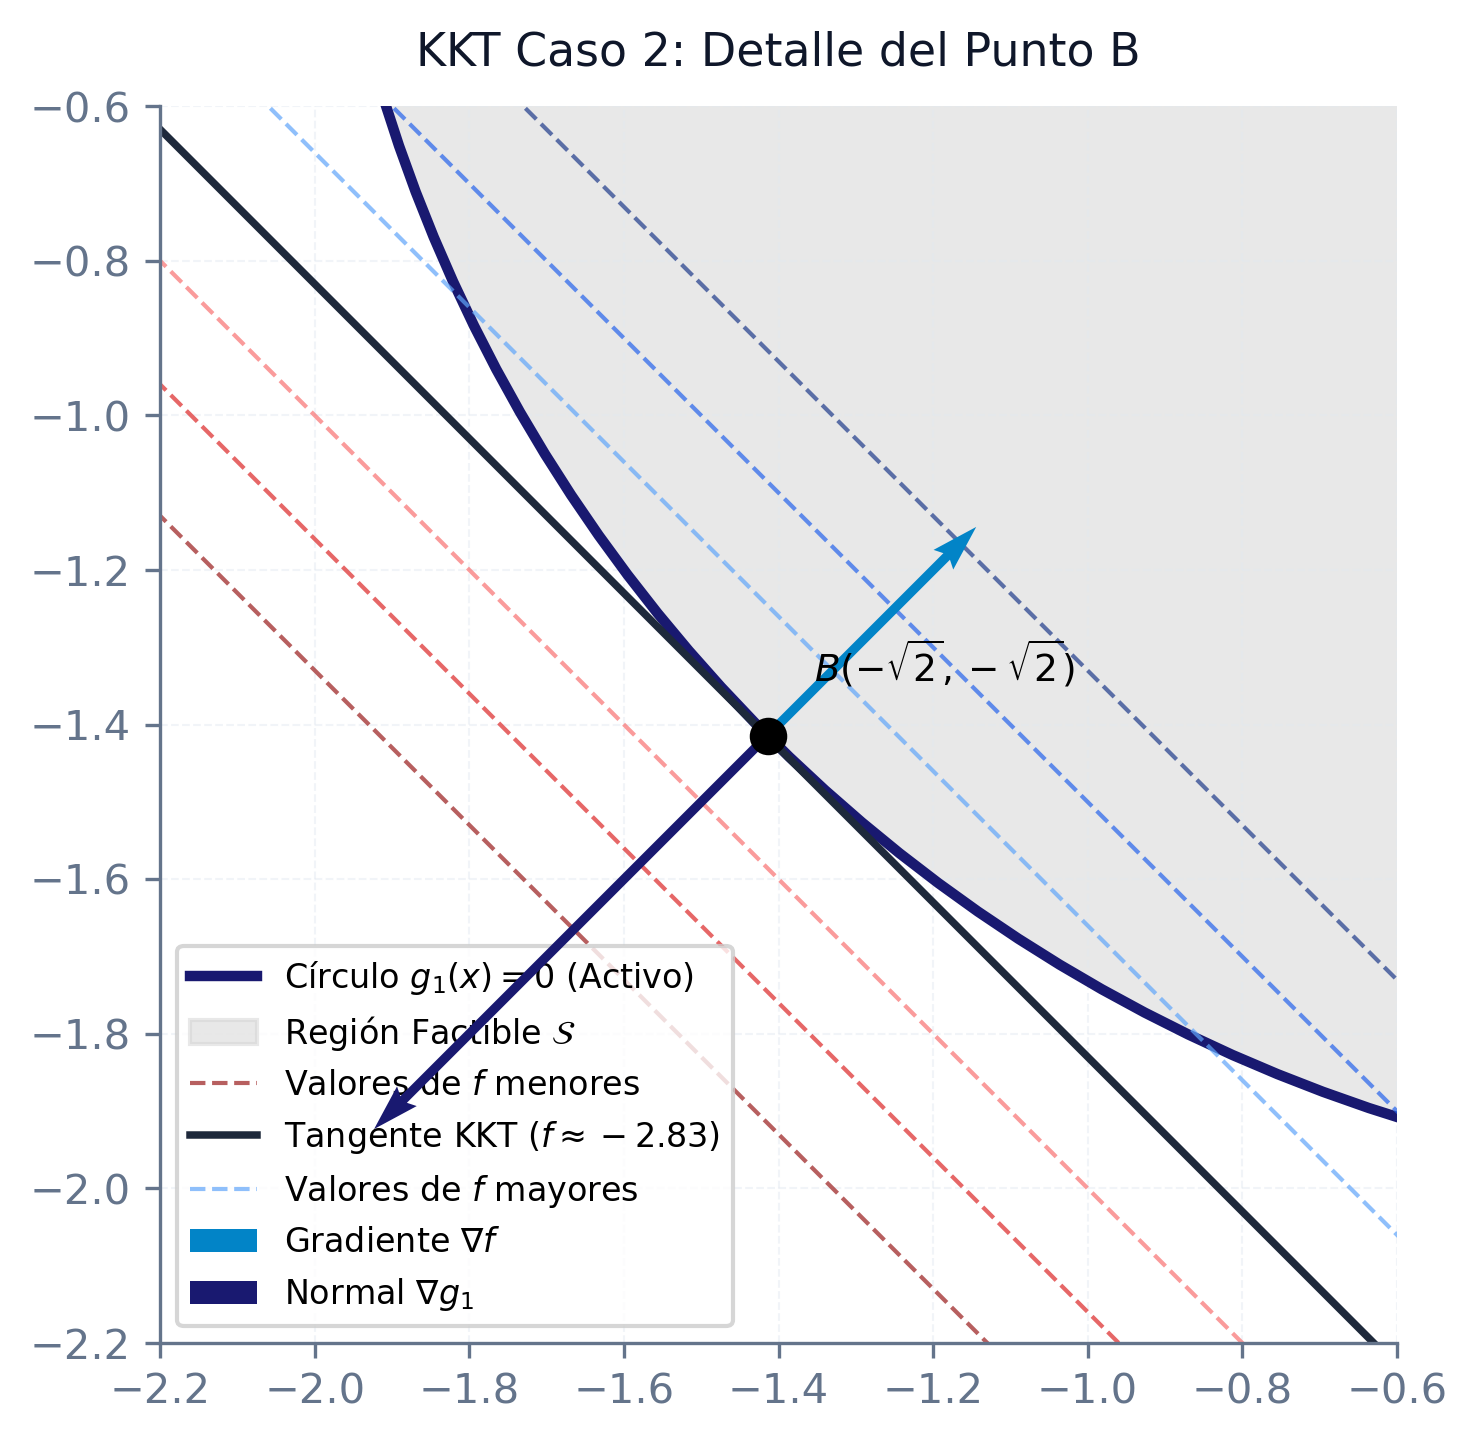
\includegraphics[keepaspectratio]{images/kkt_ejemplo_circ_parab_caso_b_detalle_b.png}}

}

\subcaption{\label{fig-kkt-ejemplo-circ-parab-caso-b-detalle-b}Detalle
del punto \(B\) (mínimo)}

\end{minipage}%
%
\begin{minipage}{0.33\linewidth}

\centering{

\pandocbounded{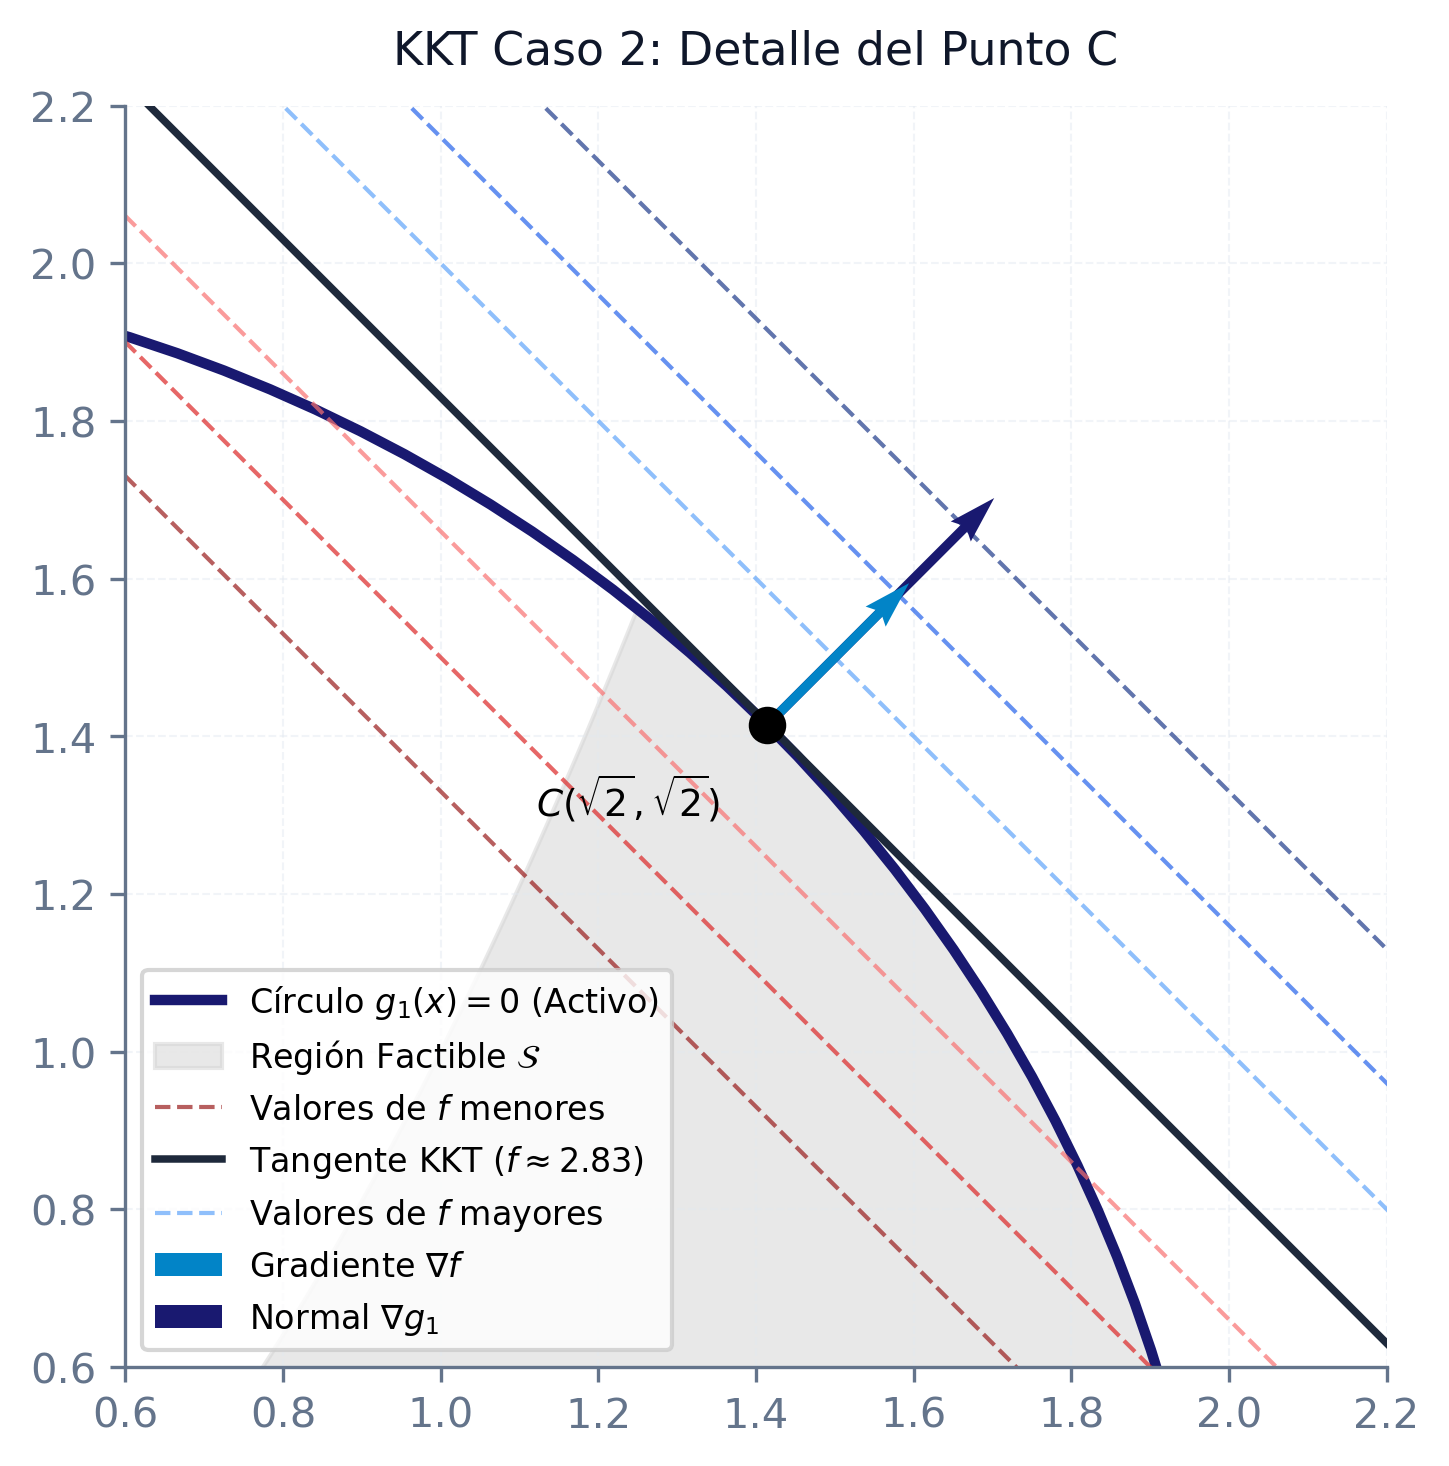
\includegraphics[keepaspectratio]{images/kkt_ejemplo_circ_parab_caso_b_detalle_c.png}}

}

\subcaption{\label{fig-kkt-ejemplo-circ-parab-caso-b-detalle-c}Detalle
del punto \(C\) (máximo)}

\end{minipage}%

\caption{\label{fig-kkt-ejemplo-circ-parab-caso-b}Caso 2: Alineación de
gradientes con parábola inactiva y círculo activo}

\end{figure}%

\begin{center}\rule{0.5\linewidth}{0.5pt}\end{center}

\textbf{Caso 3: Ambas restricciones activas
(\(u_1 \neq 0, u_2 \neq 0\))} Dado que \(u_1 \neq 0\) y \(u_2 \neq 0\),
la holgura complementaria exige que ambas restricciones sean activas
(\(g_1(x) = 0\) y \(g_2(x) = 0\)). Por lo tanto, los puntos candidatos
se encuentran en la intersección de ambas curvas, es decir, resolviendo
\(x_2 = x_1^2\) en la circunferencia:
\[ x_1^2 + (x_1^2)^2 = 4 \implies x_1^4 + x_1^2 - 4 = 0 \implies x_1^2 = \frac{-1 + \sqrt{17}}{2} \approx 1.56 \implies x_1 \approx \pm 1.25 \]
El valor de la coordenada \(x_2\) en las intersecciones es
\(x_2 = x_1^2 \approx 1.56\). Los puntos de intersección son
\(E(1.25, 1.56)\) y \(D(-1.25, 1.56)\).

Planteamos el sistema de estacionariedad para resolver \(u_1\) y
\(u_2\): \[ 1 + 2u_1 x_1 - 2u_2 x_1 = 0 \implies 2x_1(u_1 - u_2) = -1 \]
\[ 1 + 2u_1 x_2 + u_2 = 0 \]

\begin{itemize}
\tightlist
\item
  Para \(E(1.25, 1.56)\):
  \[ 2.5(u_1 - u_2) = -1 \implies u_1 - u_2 = -0.4 \implies u_2 = u_1 + 0.4 \]
  Sustituyendo en la segunda ecuación:
  \[ 1 + 2(1.56)u_1 + (u_1 + 0.4) = 0 \implies 4.12 u_1 + 1.4 = 0 \implies u_1 \approx -0.34 < 0 \]
  \[ u_2 = -0.34 + 0.4 = 0.06 > 0 \] Al tener multiplicadores con signos
  opuestos (\(u_1 < 0, u_2 > 0\)), el punto \(E\) no cumple las
  condiciones necesarias para ser ni mínimo (requiere \(u_i \ge 0\)) ni
  máximo (requiere \(u_i \le 0\)).
\item
  Para \(D(-1.25, 1.56)\):
  \[ -2.5(u_1 - u_2) = -1 \implies u_1 - u_2 = 0.4 \implies u_2 = u_1 - 0.4 \]
  Sustituyendo en la segunda ecuación:
  \[ 1 + 3.12 u_1 + u_1 - 0.4 = 0 \implies 4.12 u_1 + 0.6 = 0 \implies u_1 \approx -0.15 < 0 \]
  \[ u_2 = -0.15 - 0.4 = -0.55 < 0 \] Dado que \(u_1, u_2 < 0\), el
  punto \(D(-1.25, 1.56)\) es un \textbf{candidato a máximo local}. No
  obstante, al evaluar el valor de la función objetivo:
  \[ f(D) \approx -1.25 + 1.56 = 0.31 \] mientras que en el candidato a
  máximo global \(C\) tenemos \(f(C) = 2\sqrt{2} \approx 2.83\), y en el
  máximo local \(A\) tenemos \(f(A) = -0.5 + 0.25 = -0.25\).
\end{itemize}

Geométricamente (ver Figura~\ref{fig-kkt-ejemplo-circ-parab-caso-c}), en
la intersección \(E(1.25, 1.56)\) los vectores normales \(\nabla g_1\)
(azul oscuro) y \(\nabla g_2\) (rojo brick) apuntan en direcciones que
impiden que se contrarreste el gradiente de la función objetivo
\(\nabla f\) con multiplicadores del mismo signo, resultando en un
multiplicador del círculo negativo y uno de la parábola positivo (ver
Figura~\ref{fig-kkt-ejemplo-circ-parab-caso-c-detalle-e}). En cambio, en
la intersección \(D(-1.25, 1.56)\) sí se logra un balance con ambos
multiplicadores negativos (\(u_1, u_2 < 0\)), lo que consolida a \(D\)
como un candidato a máximo local (ver
Figura~\ref{fig-kkt-ejemplo-circ-parab-caso-c-detalle-d}).

\begin{figure}[H]

\begin{minipage}{0.33\linewidth}

\centering{

\pandocbounded{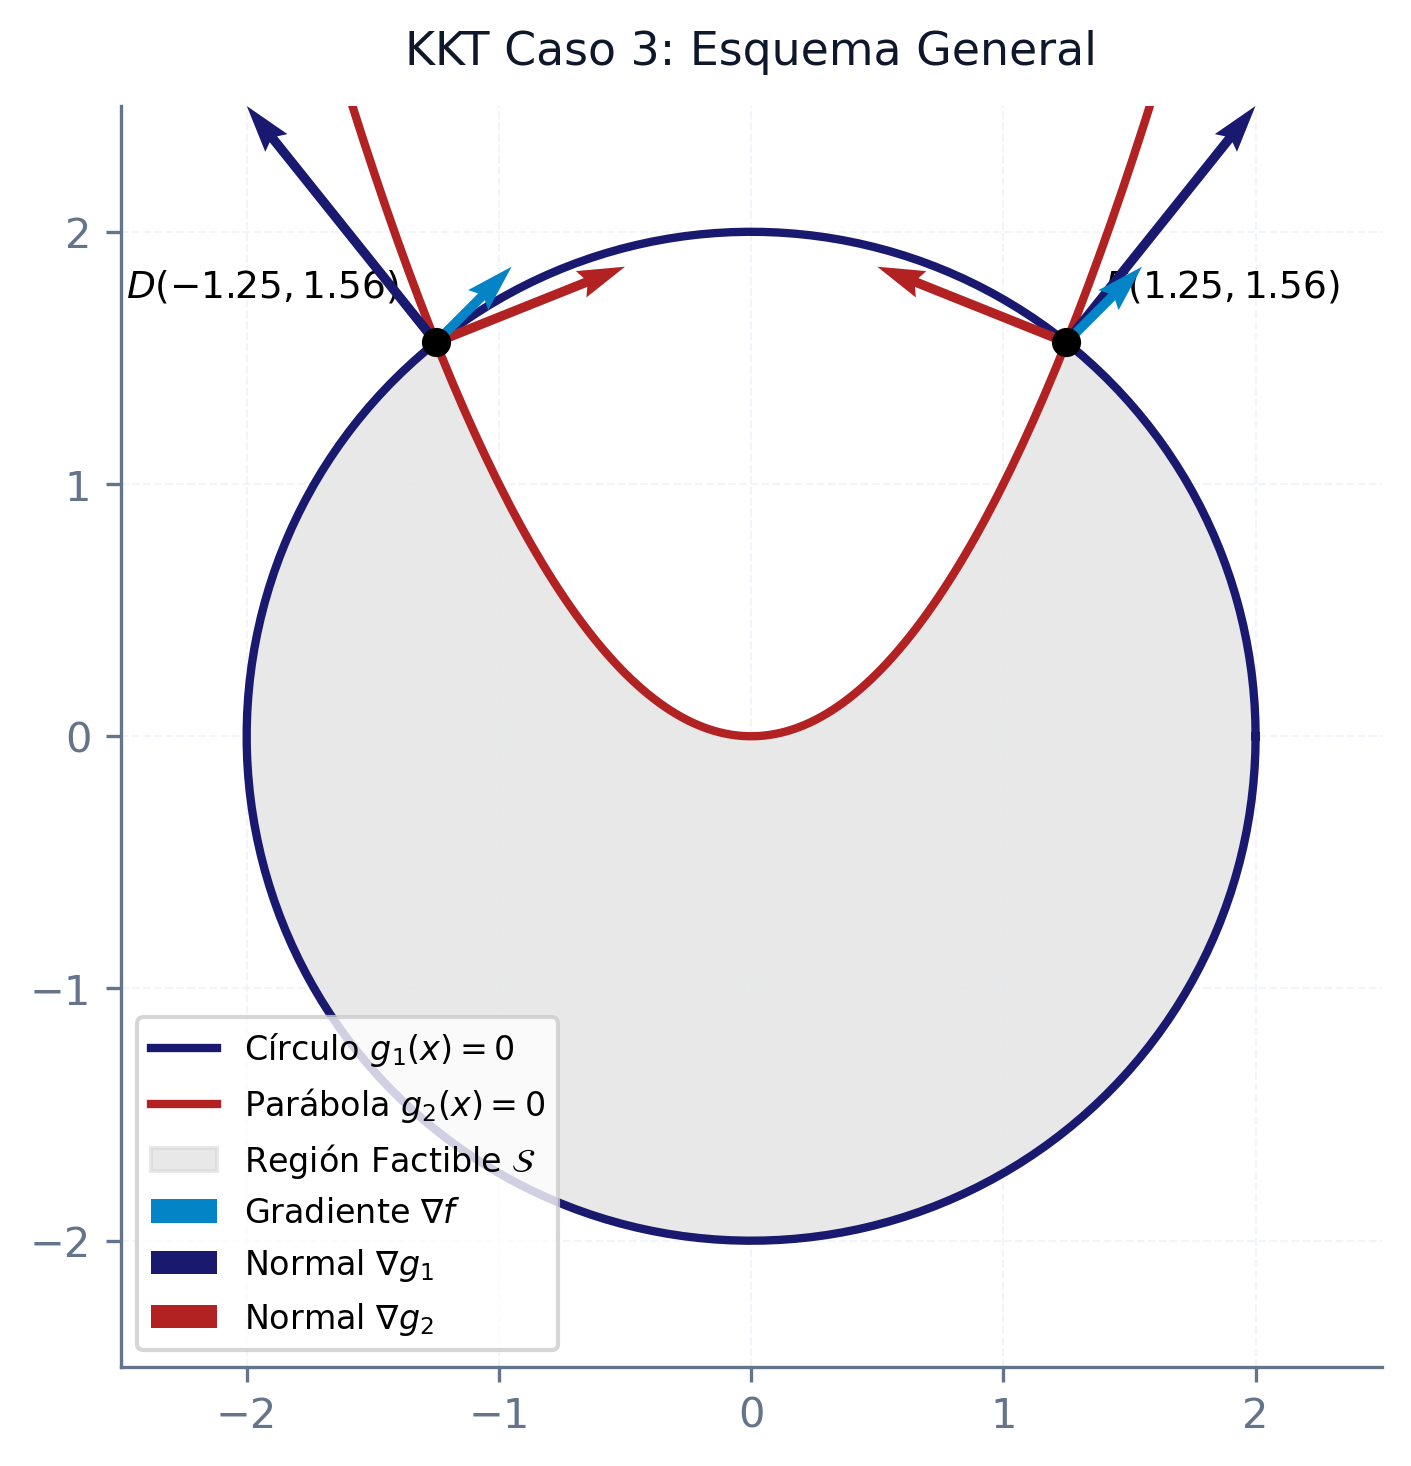
\includegraphics[keepaspectratio]{images/kkt_ejemplo_circ_parab_caso_c_general.png}}

}

\subcaption{\label{fig-kkt-ejemplo-circ-parab-caso-c-general}Esquema
general}

\end{minipage}%
%
\begin{minipage}{0.33\linewidth}

\centering{

\pandocbounded{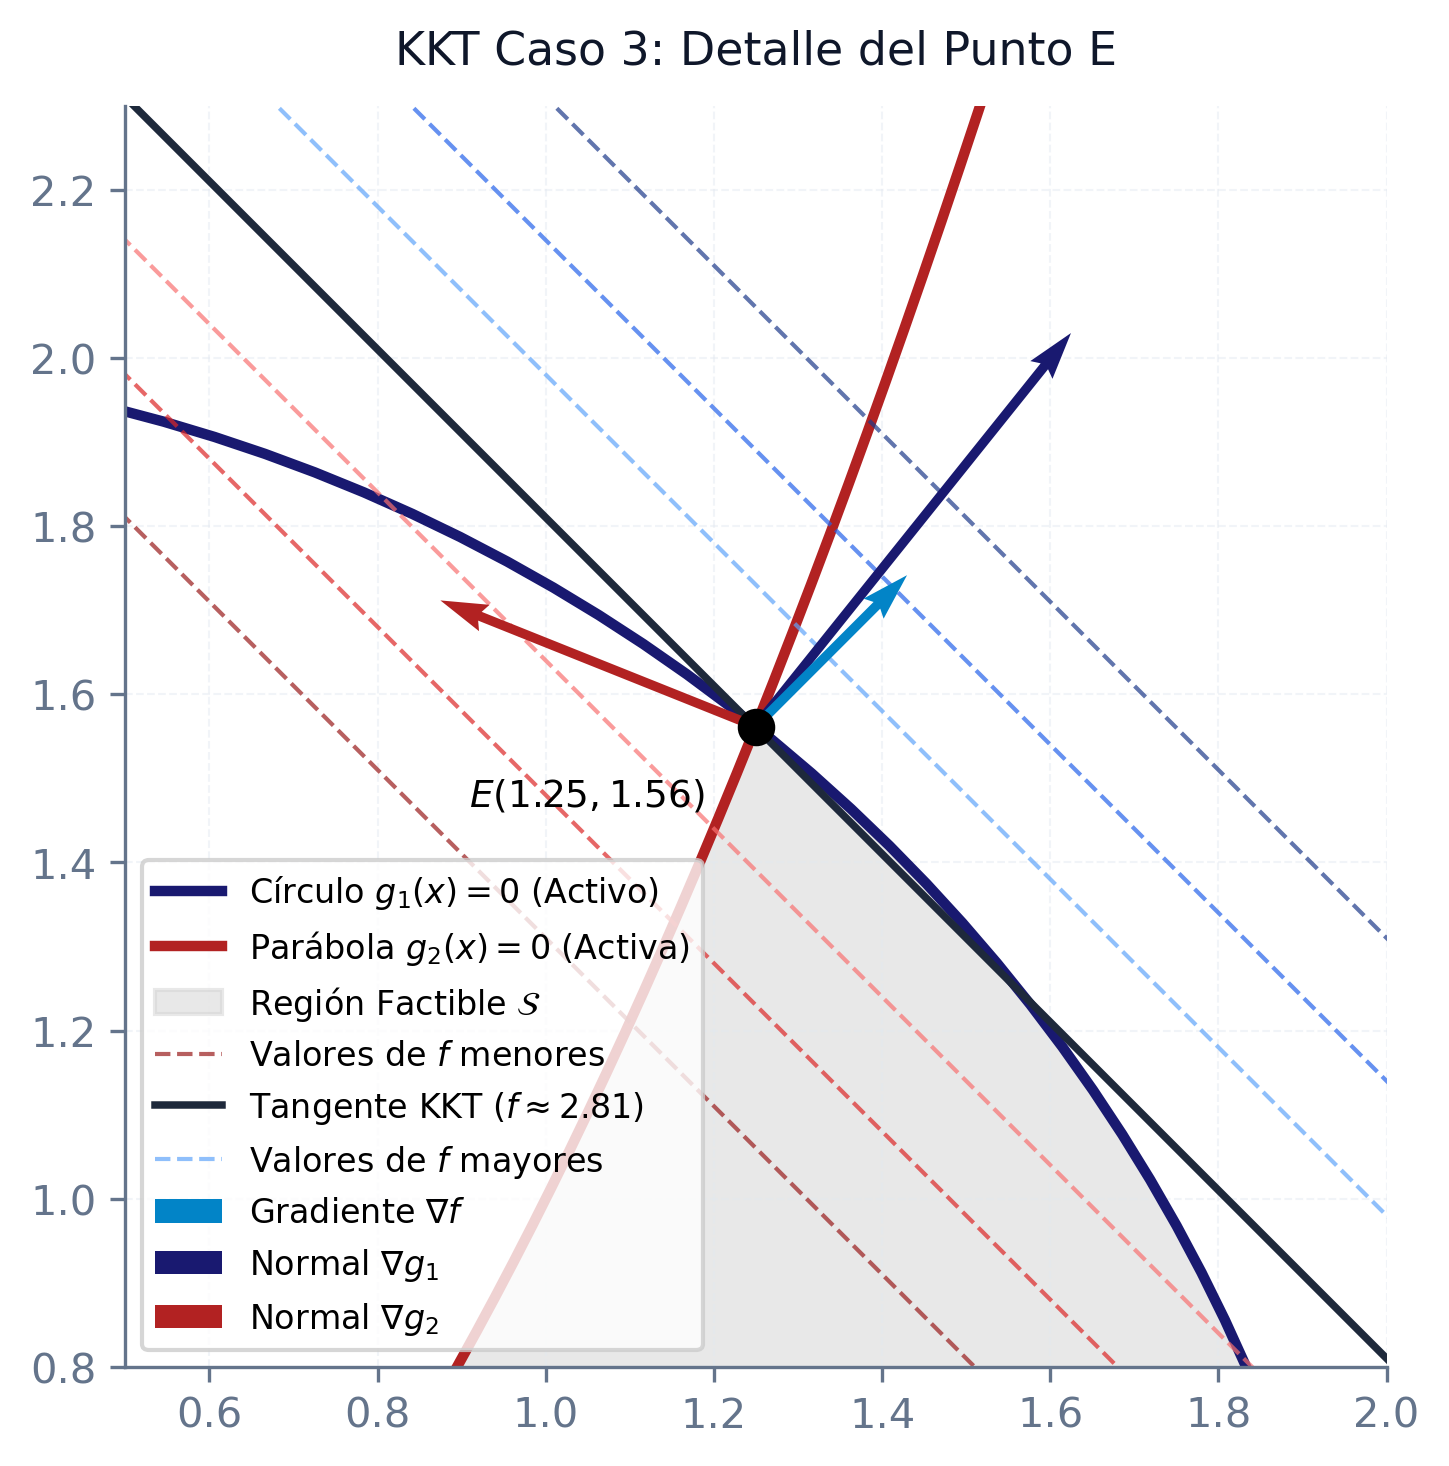
\includegraphics[keepaspectratio]{images/kkt_ejemplo_circ_parab_caso_c_detalle_e.png}}

}

\subcaption{\label{fig-kkt-ejemplo-circ-parab-caso-c-detalle-e}Detalle
del punto \(E\) (no candidato)}

\end{minipage}%
%
\begin{minipage}{0.33\linewidth}

\centering{

\pandocbounded{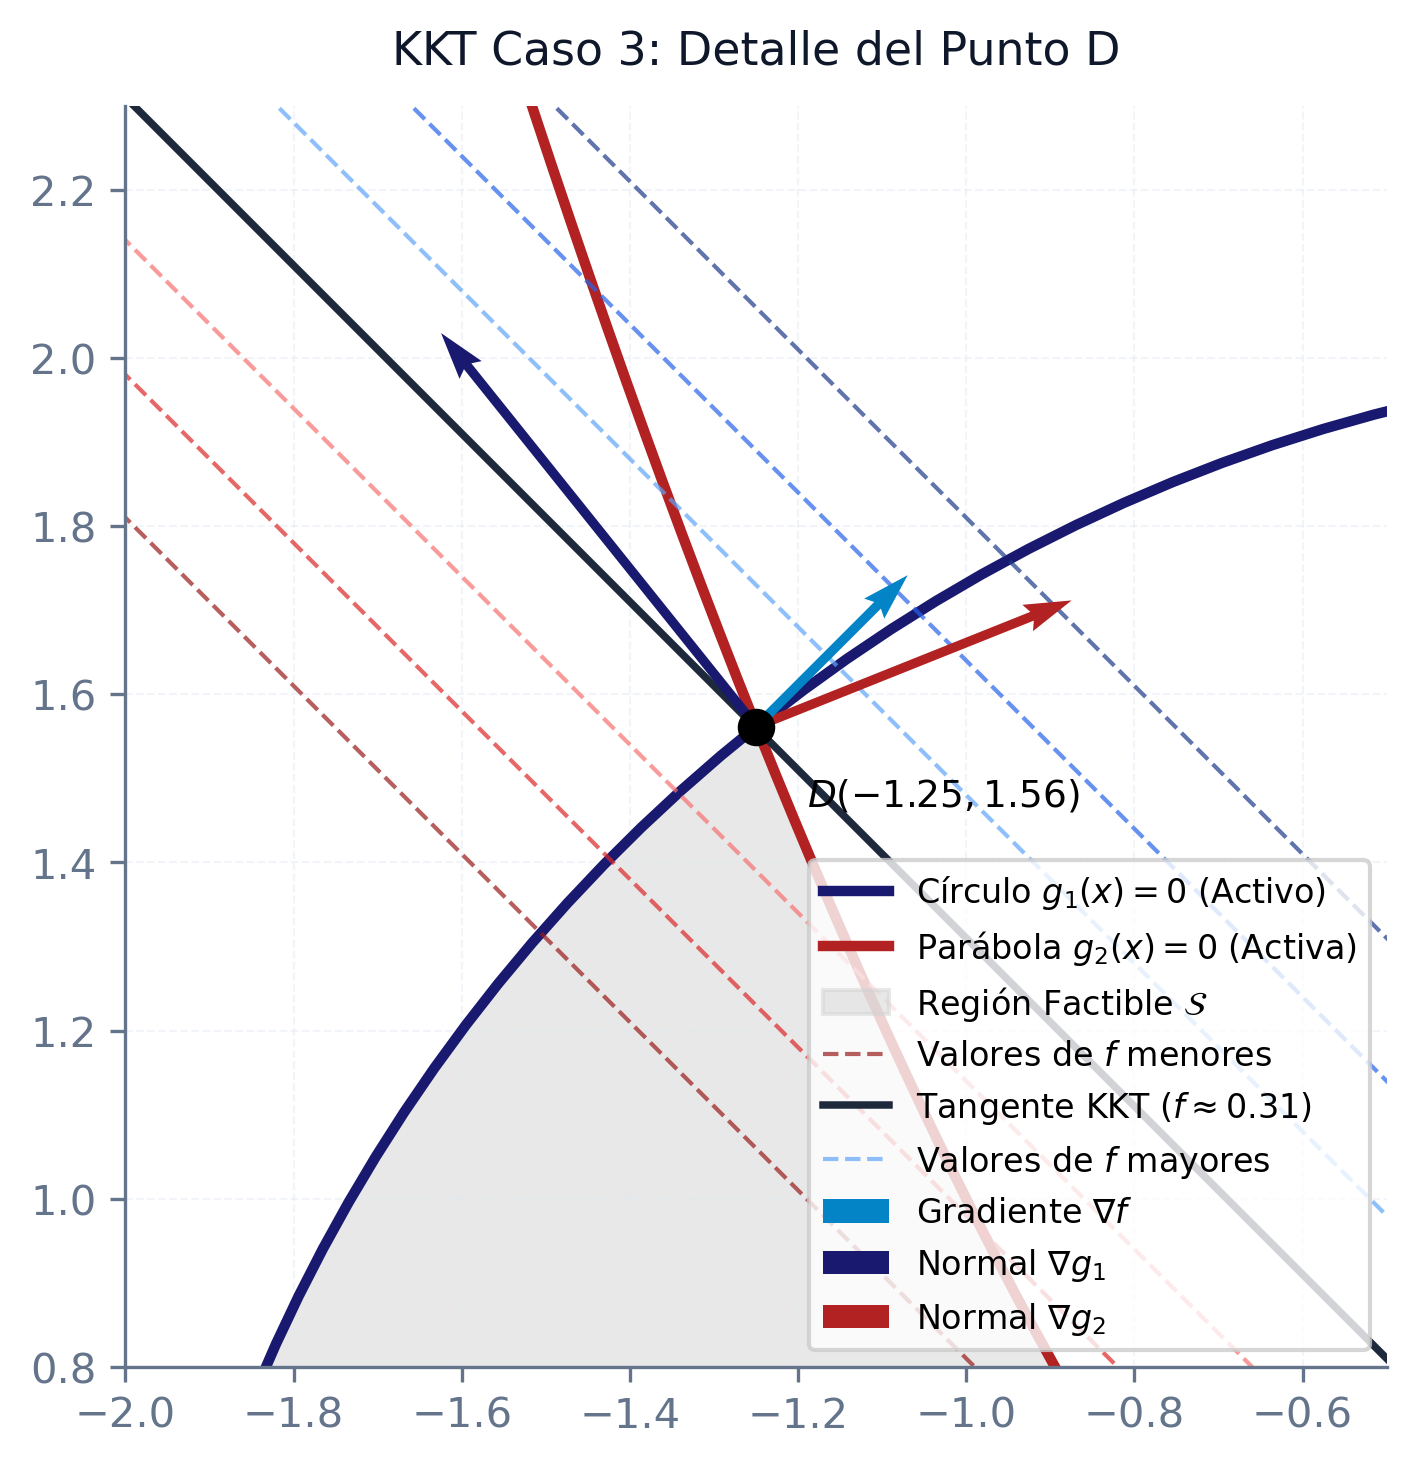
\includegraphics[keepaspectratio]{images/kkt_ejemplo_circ_parab_caso_c_detalle_d.png}}

}

\subcaption{\label{fig-kkt-ejemplo-circ-parab-caso-c-detalle-d}Detalle
del punto \(D\) (máximo local)}

\end{minipage}%

\caption{\label{fig-kkt-ejemplo-circ-parab-caso-c}Caso 3: Ambas
restricciones activas (intersección)}

\end{figure}%

\textbf{Conclusión del análisis}

Al comparar los valores de la función objetivo en los candidatos
obtenidos:

\begin{itemize}
\tightlist
\item
  \textbf{Mínimos}: El único candidato KKT es
  \(B(-\sqrt{2}, -\sqrt{2})\) con \(f(B) = -2\sqrt{2} \approx -2.83\).
  Dado que la región factible es cerrada y acotada (compacta) y las
  funciones son continuas, el teorema de Weierstrass garantiza la
  existencia de extremos globales. Por tanto, \textbf{\(B\) es el mínimo
  global}.
\item
  \textbf{Máximos}: Evaluamos los candidatos a máximo (\(u_i \le 0\)):

  \begin{itemize}
  \tightlist
  \item
    \(C(\sqrt{2}, \sqrt{2}) \implies f(C) = 2\sqrt{2} \approx 2.83\)
    (Frontera circular).
  \item
    \(D(-1.25, 1.56) \implies f(D) \approx 0.31\) (Esquina de
    intersección).
  \item
    \(A(-1/2, 1/4) \implies f(A) = -0.25\) (Descartado por análisis de
    segundo orden). Por lo tanto, \textbf{\(C(\sqrt{2}, \sqrt{2})\) es
    el máximo global} y \textbf{\(D\) es el único máximo local} (el
    punto \(A\) es un punto que no es ni máximo ni mínimo).
  \end{itemize}
\end{itemize}

\textbf{Aplicación de las condiciones suficientes de KKT}

Para corroborar analíticamente la naturaleza de estos candidatos
utilizando el teorema de suficiencia, estudiamos la curvatura de la
función objetivo y de las restricciones activas en cada caso:

\begin{itemize}
\tightlist
\item
  La función objetivo \(f(x_1, x_2) = x_1 + x_2\) es lineal y, por
  tanto, es cóncava y convexa simultáneamente en todo \(\mathbb{R}^2\).
\item
  Las matrices Hessiana de las restricciones son:
  \[ H_1 = \nabla^2 g_1(x) = \begin{pmatrix} 2 & 0 \\ 0 & 2 \end{pmatrix} \qquad \text{y} \qquad H_2 = \nabla^2 g_2(x) = \begin{pmatrix} -2 & 0 \\ 0 & 0 \end{pmatrix} \]

  \begin{itemize}
  \tightlist
  \item
    \(H_1\) es definida positiva, por lo que la restricción \(g_1\) es
    \textbf{estrictamente convexa}.
  \item
    \(H_2\) es semidefinida negativa, por lo que la restricción \(g_2\)
    es \textbf{cóncava}.
  \end{itemize}
\end{itemize}

Aplicando este análisis a cada uno de los candidatos:

\begin{itemize}
\tightlist
\item
  \textbf{Punto \(A(-1/2, 1/4)\)}:

  \begin{itemize}
  \tightlist
  \item
    Multiplicadores: \(u_1 = 0\) y \(u_2 = -1 < 0\) (candidato a
    máximo).
  \item
    Análisis: La restricción \(g_2\) es activa y cóncava.
  \item
    Conclusión: \textbf{No verifica las condiciones suficientes} de KKT
    para máximo (requeriría que \(g_2\) fuera convexa). Como vimos en el
    análisis de segundo orden, no es un extremo local.
  \end{itemize}
\item
  \textbf{Punto \(B(-\sqrt{2}, -\sqrt{2})\)}:

  \begin{itemize}
  \tightlist
  \item
    Multiplicadores: \(u_1 = \frac{\sqrt{2}}{4} > 0\) y \(u_2 = 0\)
    (candidato a mínimo).
  \item
    Análisis: La restricción \(g_1\) es activa y estrictamente convexa.
  \item
    Conclusión: Al ser \(f\) convexa y la restricción activa \(g_1\)
    convexa con multiplicador positivo, se satisfacen las condiciones
    suficientes, garantizando que \textbf{\(B\) es el mínimo global}.
  \end{itemize}
\item
  \textbf{Punto \(C(\sqrt{2}, \sqrt{2})\)}:

  \begin{itemize}
  \tightlist
  \item
    Multiplicadores: \(u_1 = -\frac{\sqrt{2}}{4} < 0\) y \(u_2 = 0\)
    (candidato a máximo).
  \item
    Análisis: La restricción \(g_1\) es activa y estrictamente convexa.
  \item
    Conclusión: Al ser \(f\) cóncava y la restricción activa \(g_1\)
    convexa con multiplicador negativo (equivalente a minimizar \(-f\)
    con restricción convexa), se satisfacen las condiciones suficientes,
    garantizando que \textbf{\(C\) es el máximo global}.
  \end{itemize}
\item
  \textbf{Punto
  \(D\left(-\sqrt{\frac{-1+\sqrt{17}}{2}}, \frac{-1+\sqrt{17}}{2}\right)\)}
  (es decir, \(D(-1.25, 1.56)\)):

  \begin{itemize}
  \tightlist
  \item
    Multiplicadores: \(u_1 \approx -0.15 < 0\) y
    \(u_2 \approx -0.55 < 0\) (candidato a máximo).
  \item
    Análisis: La restricción \(g_1\) es activa y convexa, pero la
    restricción \(g_2\) es activa y cóncava.
  \item
    Conclusión: \textbf{No verifica las condiciones suficientes} de KKT
    porque la restricción activa \(g_2\) es cóncava. No obstante,
    gráficamente se comprueba que el punto \(D\) es un \textbf{máximo
    local}.
  \end{itemize}
\end{itemize}

En la Figura~\ref{fig-kkt-ejemplo-circ-parab-conclusiones} se resume
gráficamente el resultado de la caracterización y la condición de cada
uno de los cinco candidatos estudiados.

\begin{figure}[H]

\centering{

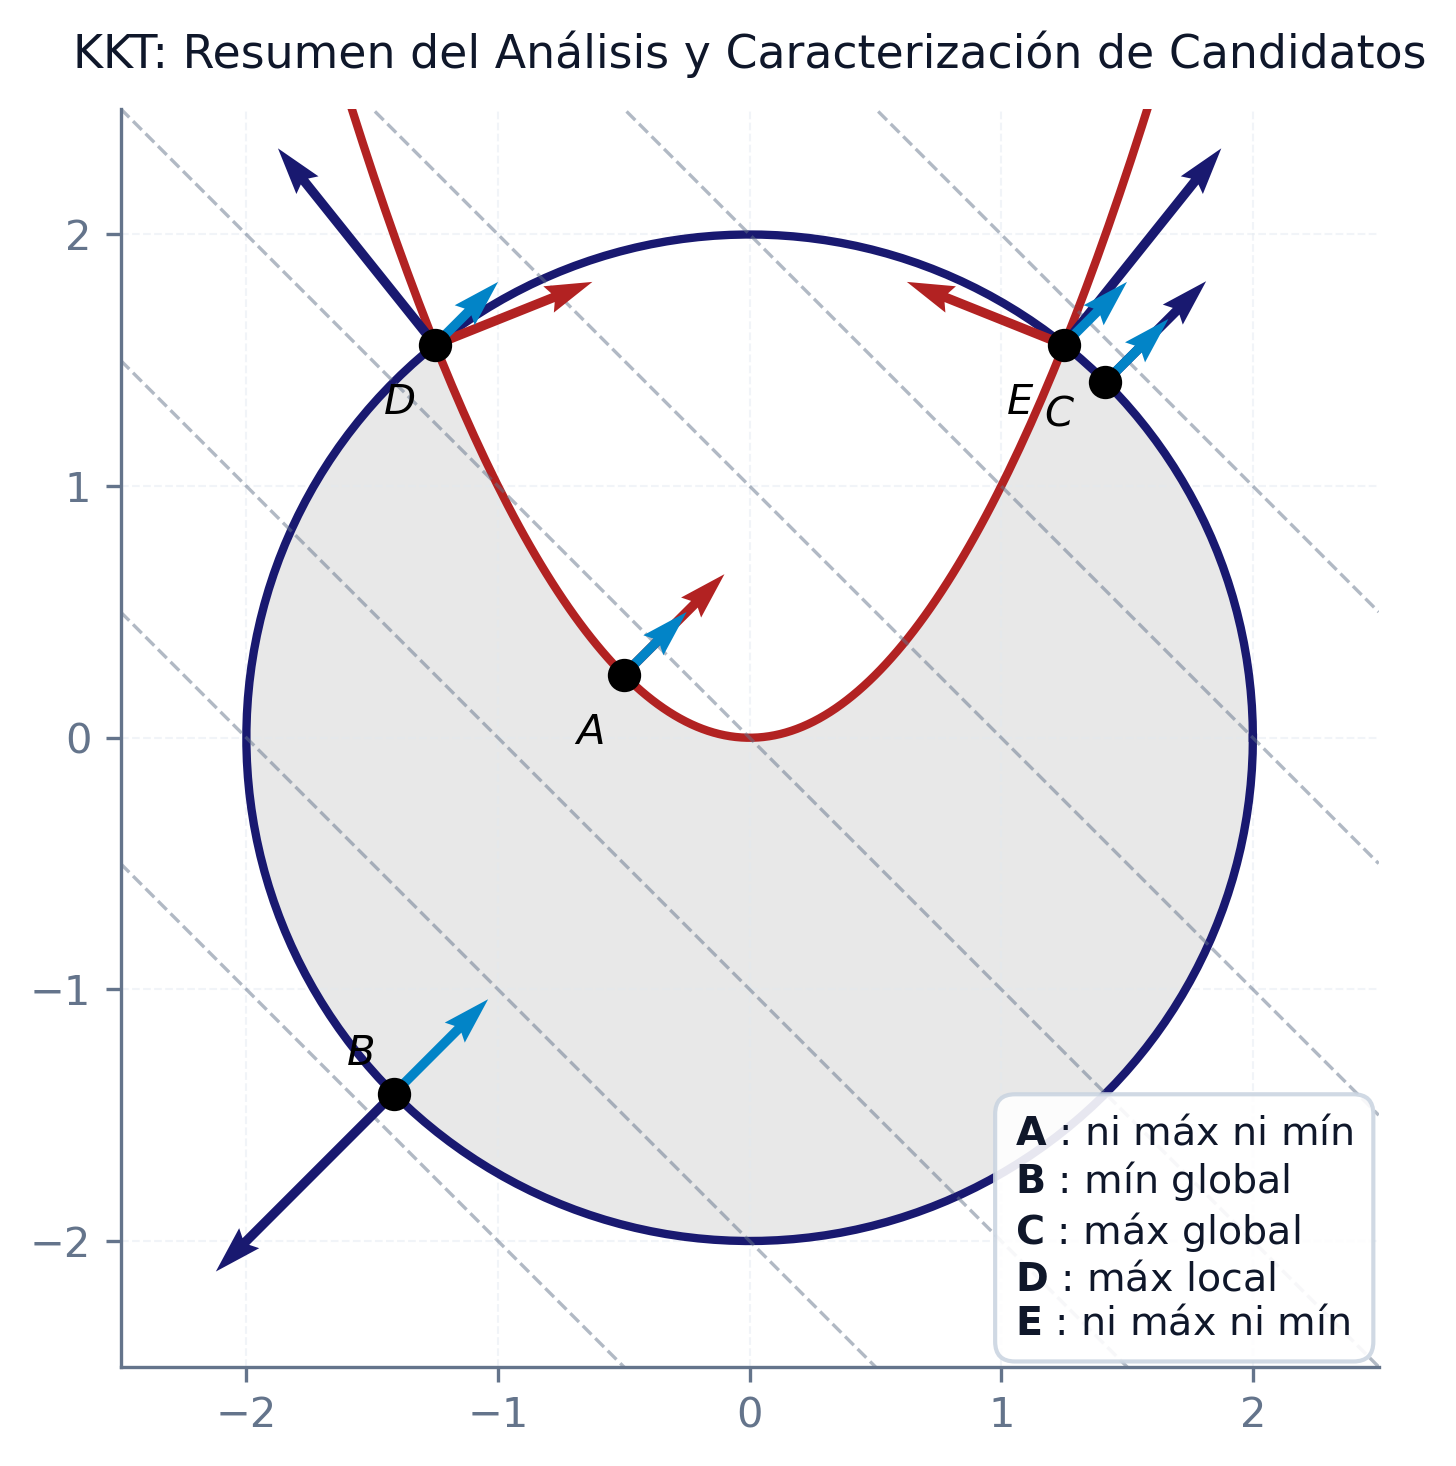
\includegraphics[width=0.75\linewidth,height=\textheight,keepaspectratio]{images/kkt_ejemplo_circ_parab_conclusiones.png}

}

\caption{\label{fig-kkt-ejemplo-circ-parab-conclusiones}KKT:
Caracterización Final de Candidatos}

\end{figure}%

\end{tcolorbox}

Con el propósito de estructurar y sistematizar la búsqueda práctica de
óptimos analíticos aplicando estas condiciones matemáticas, resulta útil
resumir todo el proceso combinatorio y de comprobación en un algoritmo
ordenado. El siguiente esquema destacado recoge las fases fundamentales
de esta estrategia:

\begin{tcolorbox}[enhanced jigsaw, toprule=.15mm, opacitybacktitle=0.6, coltitle=black, colbacktitle=quarto-callout-note-color!10!white, title=\textcolor{quarto-callout-note-color}{\faInfo}\hspace{0.5em}{Esquema general de resolución KKT}, arc=.35mm, rightrule=.15mm, toptitle=1mm, breakable, bottomtitle=1mm, titlerule=0mm, colback=white, opacityback=0, leftrule=.75mm, colframe=quarto-callout-note-color-frame, left=2mm, bottomrule=.15mm]

El procedimiento analítico para resolver problemas de optimización con
restricciones de desigualdad mediante las condiciones KKT se fundamenta
en los siguientes pasos:

\begin{enumerate}
\def\labelenumi{\arabic{enumi}.}
\tightlist
\item
  \textbf{Construir la función Lagrangiana}:
  \[ L(x, u) = f(x) + \sum_{i=1}^m u_i g_i(x) \]
\item
  \textbf{Hallar los puntos KKT}, resolviendo el sistema dual-primal
  integrado por las siguientes condiciones:

  \begin{itemize}
  \tightlist
  \item
    \textbf{Condición de gradiente (Estacionariedad / Factibilidad
    dual)}: \(\nabla_x L(x, u) = 0\) (es decir,
    \(\frac{\partial L}{\partial x_j} = 0\),
    \(\forall j = 1, \dots, n\)).
  \item
    \textbf{Condición de factibilidad (Primal)}: \(g_i(x) \le 0\),
    \(\forall i = 1, \dots, m\).
  \item
    \textbf{Condición de ortogonalidad (Holgura complementaria)}:
    \(u_i g_i(x) = 0\), \(\forall i = 1, \dots, m\).
  \item
    \textbf{Condición de no negatividad (Factibilidad dual de
    multiplicadores)}: \(u_i \ge 0\), \(\forall i = 1, \dots, m\).
  \end{itemize}
\item
  \textbf{Análisis por casos combinatorios}: Para resolver el sistema,
  para cada restricción \(i\) se evalúan las dos ramas posibles de la
  holgura complementaria:

  \begin{itemize}
  \tightlist
  \item
    \emph{Caso A (Restricción inactiva)}:
    \(g_i(x) < 0 \implies u_i = 0\).
  \item
    \emph{Caso B (Restricción activa)}:
    \(g_i(x) = 0 \implies u_i \ge 0\).
  \end{itemize}
\item
  \textbf{Descartar candidatos} que violen la factibilidad primal o que
  resulten en multiplicadores con signo incorrecto.
\item
  \textbf{Comprobar la cualificación de restricciones (LICQ)} en los
  candidatos y aplicar las \textbf{condiciones suficientes por
  convexidad} (si las restricciones activas \(g_i\) son cuasi-convexas
  diferenciables y la función objetivo \(f\) es pseudo-convexa en el
  candidato, este es un mínimo global; en caso contrario, se debe
  realizar un análisis individual de los puntos, incluyendo los puntos
  singulares excluidos donde LICQ falla).
\end{enumerate}

\emph{Observaciones adicionales}:

\begin{itemize}
\tightlist
\item
  \textbf{Problemas de Maximización}: El único cambio en este
  procedimiento consiste en exigir que los multiplicadores de Lagrange
  sean no positivos (\(u_i \le 0\), \(\forall i = 1, \dots, m\)).
\item
  \textbf{Identificación de puntos Fritz-John}: Los puntos de Fritz-John
  corresponden a la generalización dual. Para identificarlos todos, se
  deben distinguir los casos en los que \(u_0 > 0\) (que equivalen a los
  puntos KKT hallados) y aquellos en los que \(u_0 = 0\) (puntos
  Fritz-John estrictos/singulares donde falla la cualificación de
  restricciones y la función objetivo no interviene).
\end{itemize}

\end{tcolorbox}

\begin{tcolorbox}[enhanced jigsaw, toprule=.15mm, opacitybacktitle=0.6, coltitle=black, colbacktitle=quarto-callout-tip-color!10!white, title=\textcolor{quarto-callout-tip-color}{\faLightbulb}\hspace{0.5em}{Ejemplo: Optimización con múltiples restricciones de desigualdad}, arc=.35mm, rightrule=.15mm, toptitle=1mm, breakable, bottomtitle=1mm, titlerule=0mm, colback=white, opacityback=0, leftrule=.75mm, colframe=quarto-callout-tip-color-frame, left=2mm, bottomrule=.15mm]

Consideremos el problema de encontrar los mínimos y máximos locales y
globales de: \[
\begin{aligned}
\min/\max \quad & f(x, y) = \left(x - \frac{9}{4}\right)^2 + (y - 2)^2 \\
\text{s.a.} \quad & g_1(x, y) = -x + y^2 \le 0 \\
& g_2(x, y) = x + y - 6 \le 0 \\
& g_3(x, y) = -x \le 0 \\
& g_4(x, y) = -y \le 0
\end{aligned}
\]

El gradiente de la función objetivo y de las restricciones son: \[
\nabla f = \begin{pmatrix} 2\left(x - \frac{9}{4}\right) \\ 2(y - 2) \end{pmatrix}, \quad \nabla g_1 = \begin{pmatrix} -1 \\ 2y \end{pmatrix}, \quad \nabla g_2 = \begin{pmatrix} 1 \\ 1 \end{pmatrix}, \quad \nabla g_3 = \begin{pmatrix} -1 \\ 0 \end{pmatrix}, \quad \nabla g_4 = \begin{pmatrix} 0 \\ -1 \end{pmatrix}
\]

La función Lagrangiana es:
\[ L(x, y, u) = \left(x - \frac{9}{4}\right)^2 + (y - 2)^2 + u_1(-x + y^2) + u_2(x + y - 6) - u_3 x - u_4 y \]

El sistema de condiciones KKT se plantea como:

\begin{enumerate}
\def\labelenumi{\arabic{enumi}.}
\tightlist
\item
  \textbf{Estacionariedad (Factibilidad dual)}:
  \[ \frac{\partial L}{\partial x} = 2\left(x - \frac{9}{4}\right) - u_1 + u_2 - u_3 = 0 \]
  \[ \frac{\partial L}{\partial y} = 2(y - 2) + 2y u_1 + u_2 - u_4 = 0 \]
\item
  \textbf{Factibilidad primal}:
  \[ -x + y^2 \le 0, \quad x + y - 6 \le 0, \quad -x \le 0, \quad -y \le 0 \]
\item
  \textbf{Ortogonalidad (Holgura complementaria)}:
  \[ u_1(-x + y^2) = 0, \quad u_2(x + y - 6) = 0, \quad u_3 x = 0, \quad u_4 y = 0 \]
\item
  \textbf{Signo de los multiplicadores}:

  \begin{itemize}
  \tightlist
  \item
    Para \textbf{mínimos}: \(u_i \ge 0, \ \forall i = 1, \dots, m\).
  \item
    Para \textbf{máximos}: \(u_i \le 0, \ \forall i = 1, \dots, m\).
  \end{itemize}
\end{enumerate}

Geométricamente, el problema representa la minimización o maximización
de la distancia al punto \((2.25, 2)^T\) sobre la región factible
delimitada por una parábola, una recta y los ejes de coordenadas (ver
Figura~\ref{fig-kkt-ejemplo-multiple-general}).

\begin{figure}[H]

\centering{

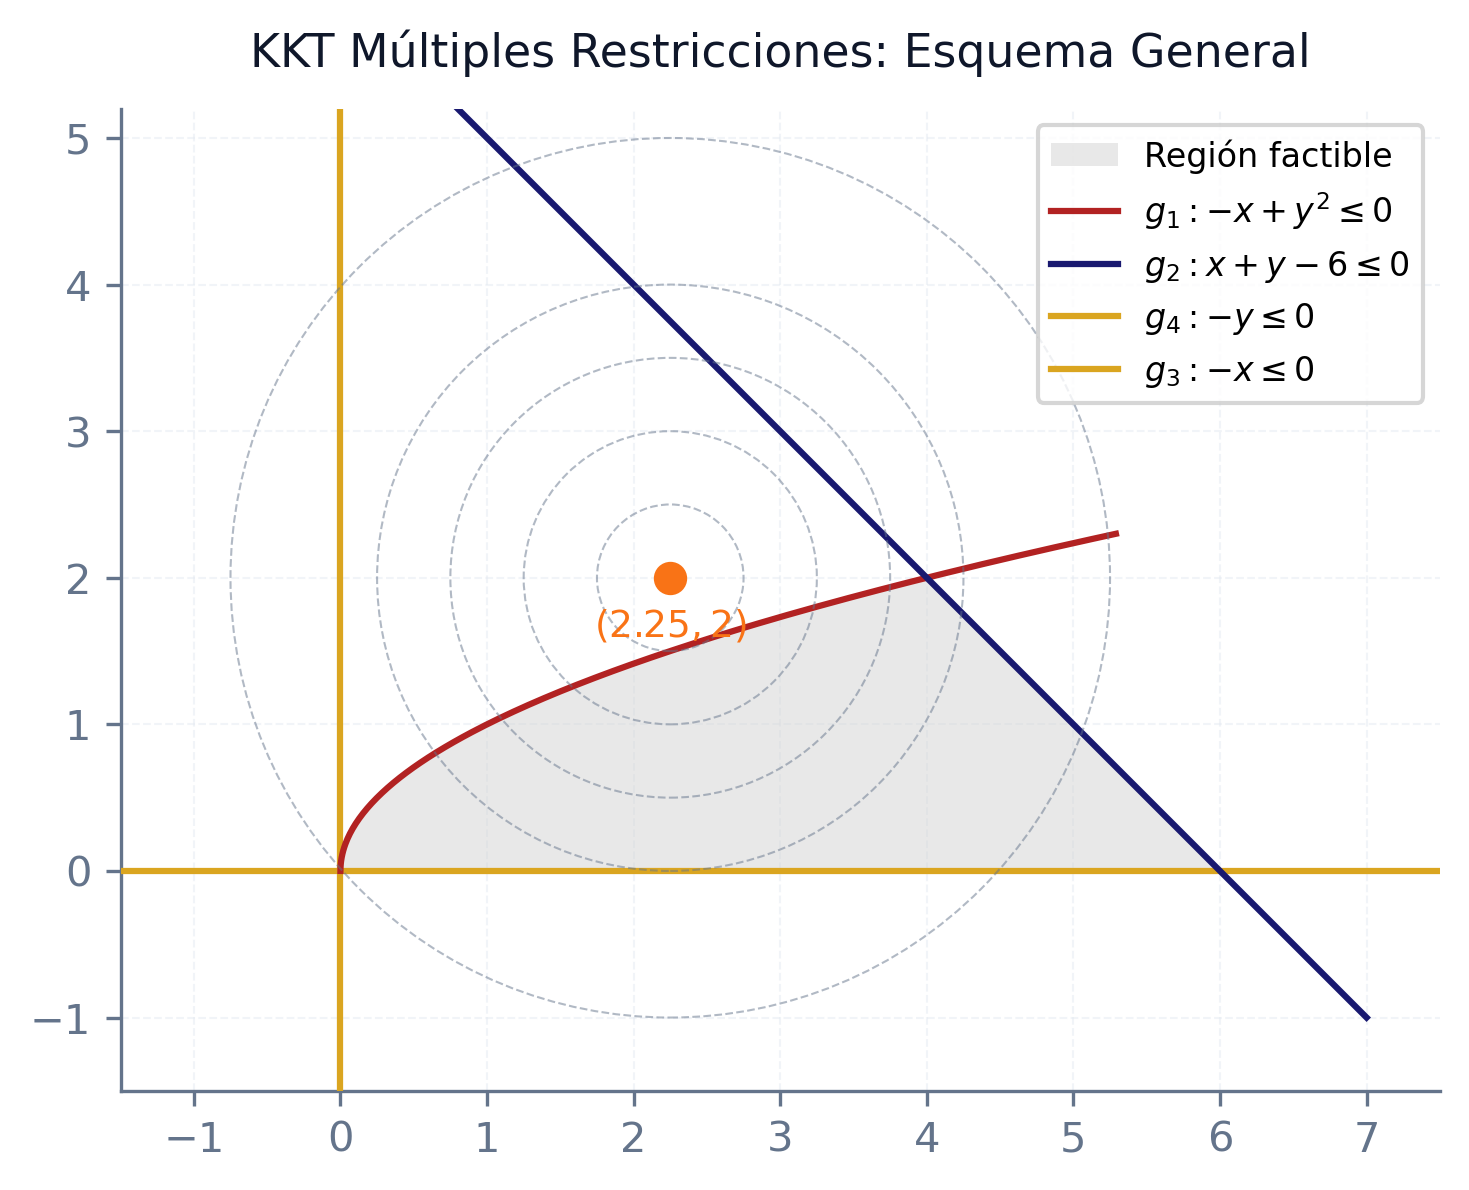
\includegraphics[width=0.6\linewidth,height=\textheight,keepaspectratio]{images/kkt_ejemplo_multiple_desigualdad.png}

}

\caption{\label{fig-kkt-ejemplo-multiple-general}KKT Múltiples
Restricciones: Esquema General}

\end{figure}%

\textbf{Resolución combinatoria por casos}

Analizamos las combinaciones de restricciones activas e inactivas
mediante la holgura complementaria:

\begin{itemize}
\item
  \textbf{Caso 1: Todas las restricciones inactivas
  (\(u_1 = u_2 = u_3 = u_4 = 0\))}: De las ecuaciones de estacionariedad
  obtenemos de forma inmediata \(x = 9/4 = 2.25\) e \(y = 2\).
  Verificamos la factibilidad primal en la primera restricción:
  \[ g_1(2.25, 2) = -2.25 + 4 = 1.75 > 0 \quad (\text{no factible}) \]
  Por lo tanto, el punto \((2.25, 2)^T\) se descarta.
\item
  \textbf{Caso 2: Una única restricción activa}:

  \begin{itemize}
  \item
    \emph{Subcaso \(g_1\) activa (\(u_1 \neq 0, u_2=u_3=u_4=0\))}: El
    sistema de estacionariedad es:
    \[ 2(x - 2.25) - u_1 = 0 \implies u_1 = 2x - 4.5 \]
    \[ 2(y - 2) + 2y u_1 = 0 \implies 2y - 4 + 2y(2x - 4.5) = 0 \implies 4xy - 7y - 4 = 0 \]
    Como \(g_1\) es activa, se cumple \(x = y^2\). Sustituyendo en la
    ecuación: \[ 4y^3 - 7y - 4 = 0 \] La única raíz real de esta
    ecuación cúbica es \(y \approx 1.55\), lo que nos da
    \(x = y^2 \approx 2.40\). Calculamos el multiplicador:
    \(u_1 = 2(2.40) - 4.5 = 0.30 > 0\). Comprobamos la factibilidad
    primal en el resto de restricciones:
    \[ g_2(2.40, 1.55) = 2.40 + 1.55 - 6 = -2.05 \le 0 \quad (\text{factible}) \]
    Dado que \(u_1 = 0.30 \ge 0\), el punto \textbf{\((2.40, 1.55)\)} es
    un candidato a mínimo local (ver detalle en
    Figura~\ref{fig-kkt-ejemplo-multiple-zoom-d}).

    \begin{figure}[H]

    \centering{

    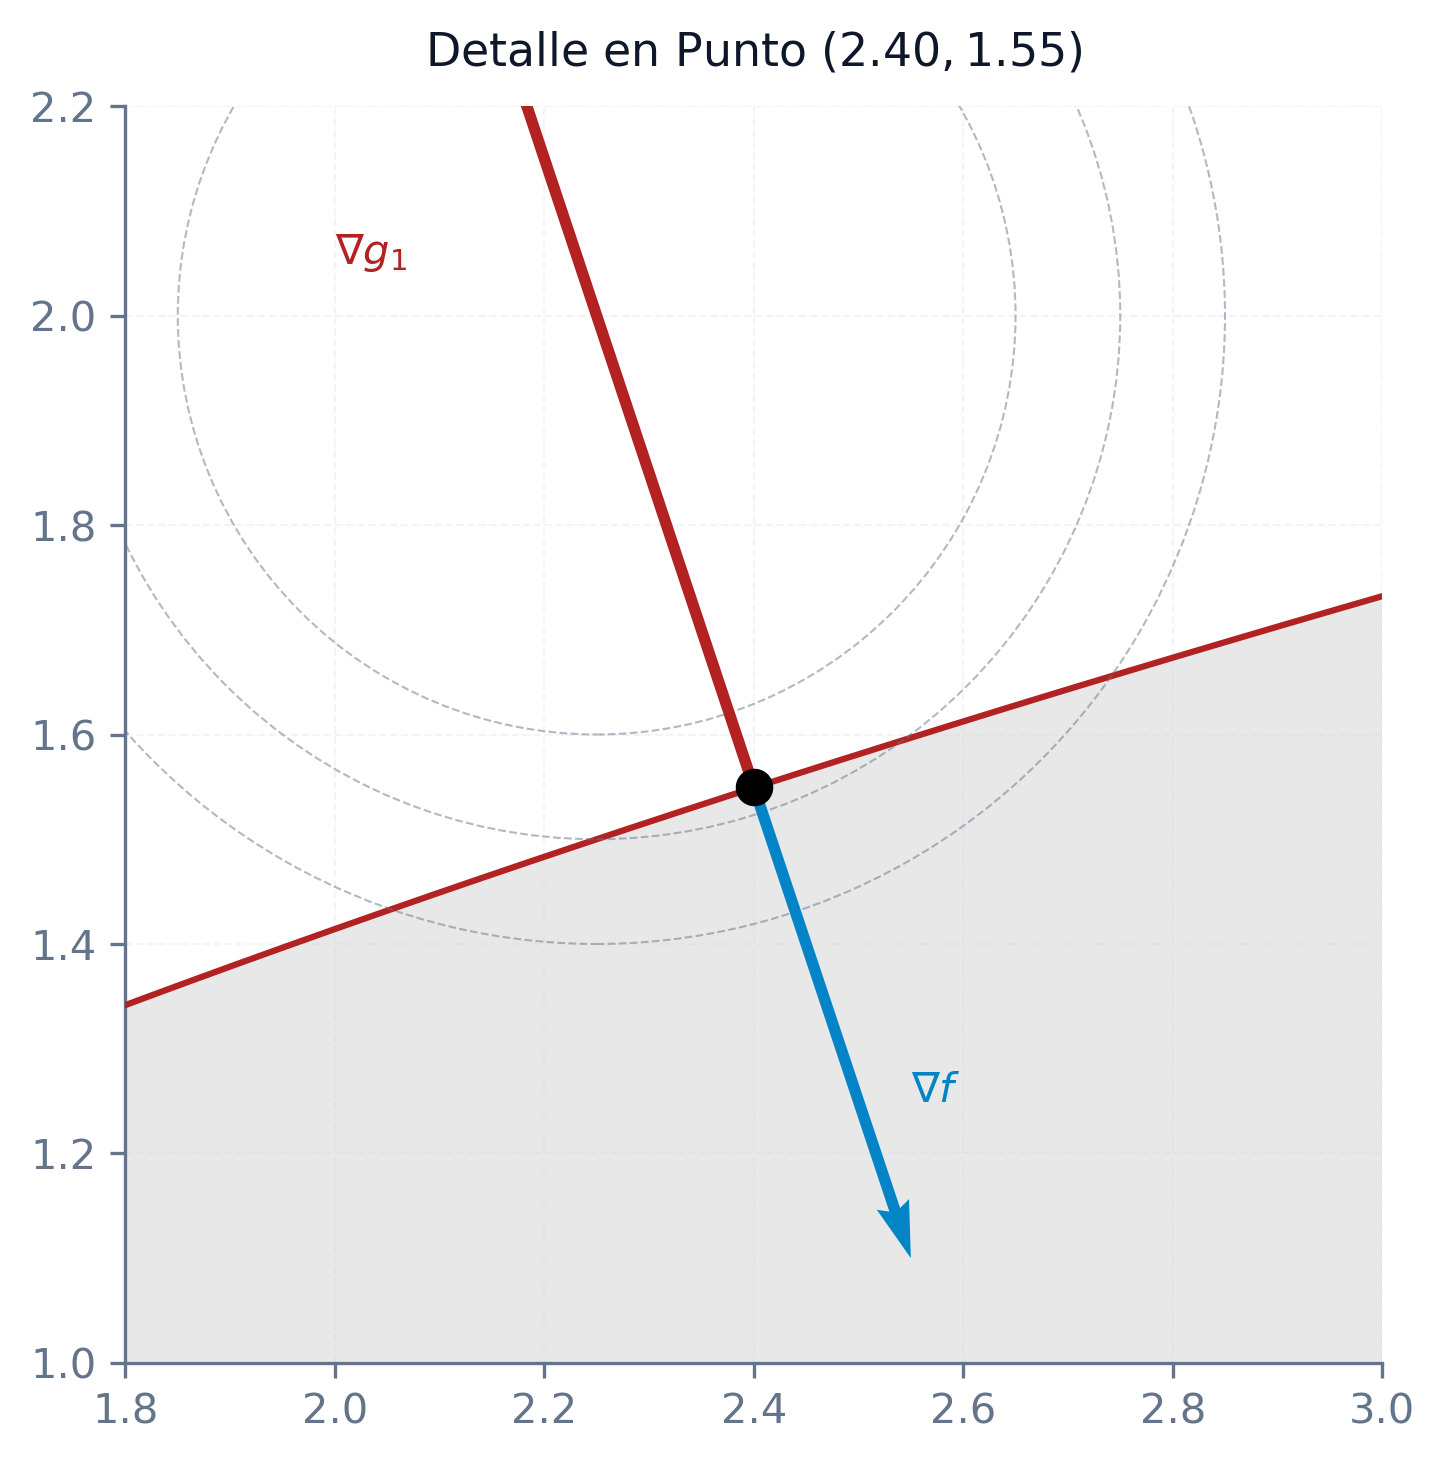
\includegraphics[width=0.6\linewidth,height=\textheight,keepaspectratio]{images/kkt_ejemplo_multiple_zoom_d.png}

    }

    \caption{\label{fig-kkt-ejemplo-multiple-zoom-d}KKT Múltiples
    Restricciones: Detalle en \((2.40, 1.55)\)}

    \end{figure}%
  \item
    \emph{Subcaso \(g_2\) activa (\(u_2 \neq 0, u_1=u_3=u_4=0\))}: El
    sistema es:
    \[ 2(x - 2.25) + u_2 = 0 \qquad \text{y} \qquad 2(y - 2) + u_2 = 0 \implies x - 2.25 = y - 2\]
    \[\implies x = y + 0.25 \] Como \(g_2\) es activa,
    \(x + y = 6 \implies y + 0.25 + y = 6 \implies 2y = 5.75 \implies y = 2.875\),
    lo que da \(x = 3.125\). Calculamos el multiplicador:
    \(u_2 = -2(3.125 - 2.25) = -1.75 < 0\). Al ser negativo, es
    candidato a máximo, pero debemos comprobar la factibilidad primal:
    \[ g_1(3.125, 2.875) = -3.125 + (2.875)^2 \approx -3.125 + 8.27 = 5.14 > 0 \quad (\text{no factible}) \]
    Por lo tanto, se descarta.
  \item
    \emph{Subcaso \(g_3\) activa (\(u_3 \neq 0, u_1=u_2=u_4=0\))}: Gives
    \(x = 0\) y \(2(y - 2) = 0 \implies y = 2\). El multiplicador es
    \(u_3 = 2(0 - 2.25) = -4.5 < 0\). Verificamos factibilidad en
    \(g_1\): \[ g_1(0, 2) = 0 + 4 = 4 > 0 \quad (\text{no factible}) \]
    Por lo tanto, se descarta.
  \item
    \emph{Subcaso \(g_4\) activa (\(u_4 \neq 0, u_1=u_2=u_3=0\))}: Gives
    \(y = 0\) y \(2(x - 2.25) = 0 \implies x = 2.25\). El multiplicador
    es \(u_4 = 2(0 - 2) + u_2 = 2(0 - 2) + 0 = -4 < 0\) (candidato a
    máximo). Comprobamos la factibilidad primal:
    \[ g_1(2.25, 0) = -2.25 + 0 = -2.25 \le 0 \quad (\text{factible}) \]
    \[ g_2(2.25, 0) = 2.25 + 0 - 6 = -3.75 \le 0 \quad (\text{factible}) \]
    Por lo tanto, el punto \textbf{\((2.25, 0)\)} es un candidato a
    máximo local (ver detalle en
    Figura~\ref{fig-kkt-ejemplo-multiple-zoom-a}).

    \begin{figure}[H]

    \centering{

    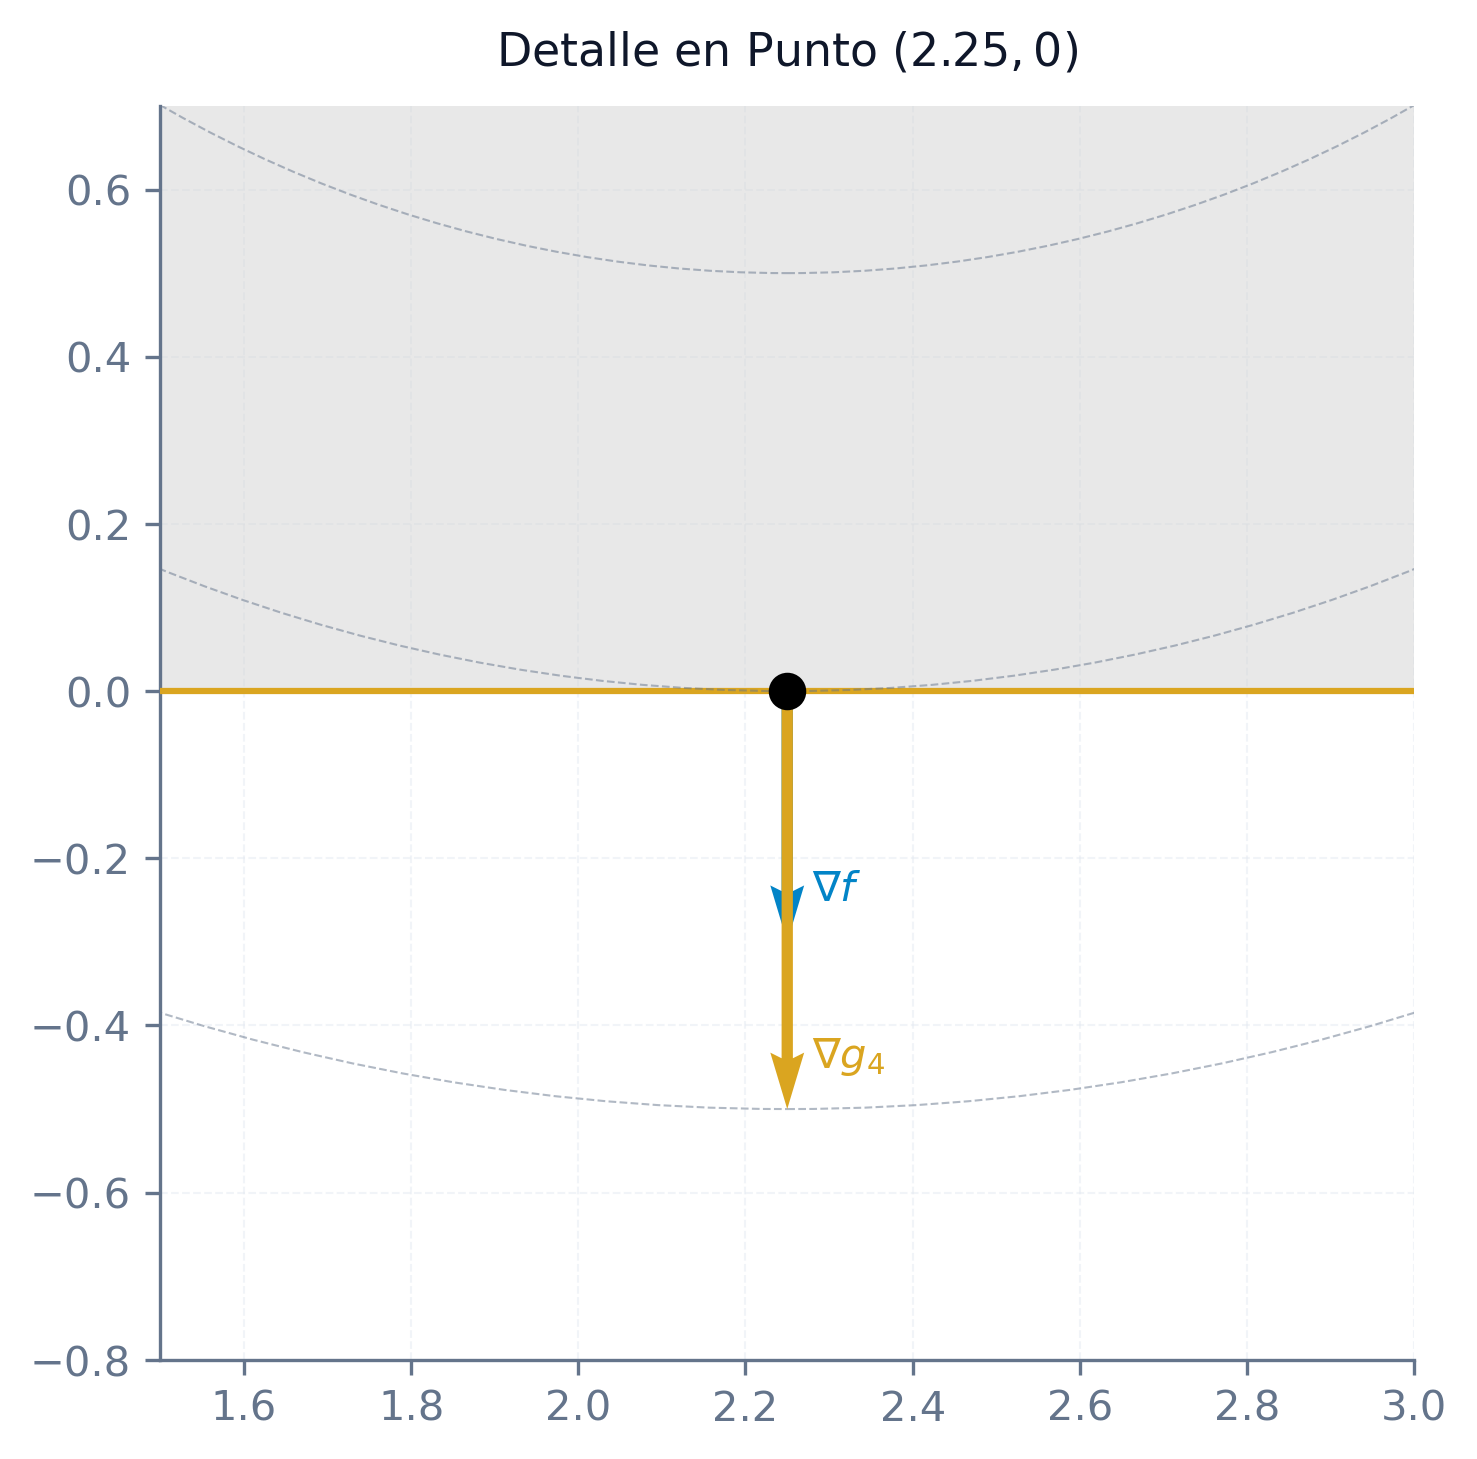
\includegraphics[width=0.6\linewidth,height=\textheight,keepaspectratio]{images/kkt_ejemplo_multiple_zoom_a.png}

    }

    \caption{\label{fig-kkt-ejemplo-multiple-zoom-a}KKT Múltiples
    Restricciones: Detalle en \((2.25, 0)\)}

    \end{figure}%
  \end{itemize}
\item
  \textbf{Caso 3: Dos restricciones activas}:

  \begin{itemize}
  \item
    \emph{Subcaso \(g_1, g_2\) activas
    (\(u_1 \neq 0, u_2 \neq 0, u_3=u_4=0\))}: Intersección de la
    parábola y la recta: \(x = y^2\) y
    \(x+y=6 \implies y^2+y-6=0 \implies y=2\) (puesto que \(y \ge 0\)),
    lo que da \(x=4\). El sistema de estacionariedad queda:
    \[ 2(4 - 2.25) - u_1 + u_2 = 0 \implies 3.5 - u_1 + u_2 = 0 \]
    \[ 2(2 - 2) + 4u_1 + u_2 = 0 \implies 4u_1 + u_2 = 0 \implies u_2 = -4u_1 \]
    Sustituyendo: \(3.5 - 5u_1 = 0 \implies u_1 = 0.70 > 0\) y
    \(u_2 = -2.80 < 0\). Al tener signos opuestos, el punto
    \textbf{\((4, 2)\)} no es candidato a mínimo ni a máximo (ver
    detalle en Figura~\ref{fig-kkt-ejemplo-multiple-zoom-e}).

    \begin{figure}[H]

    \centering{

    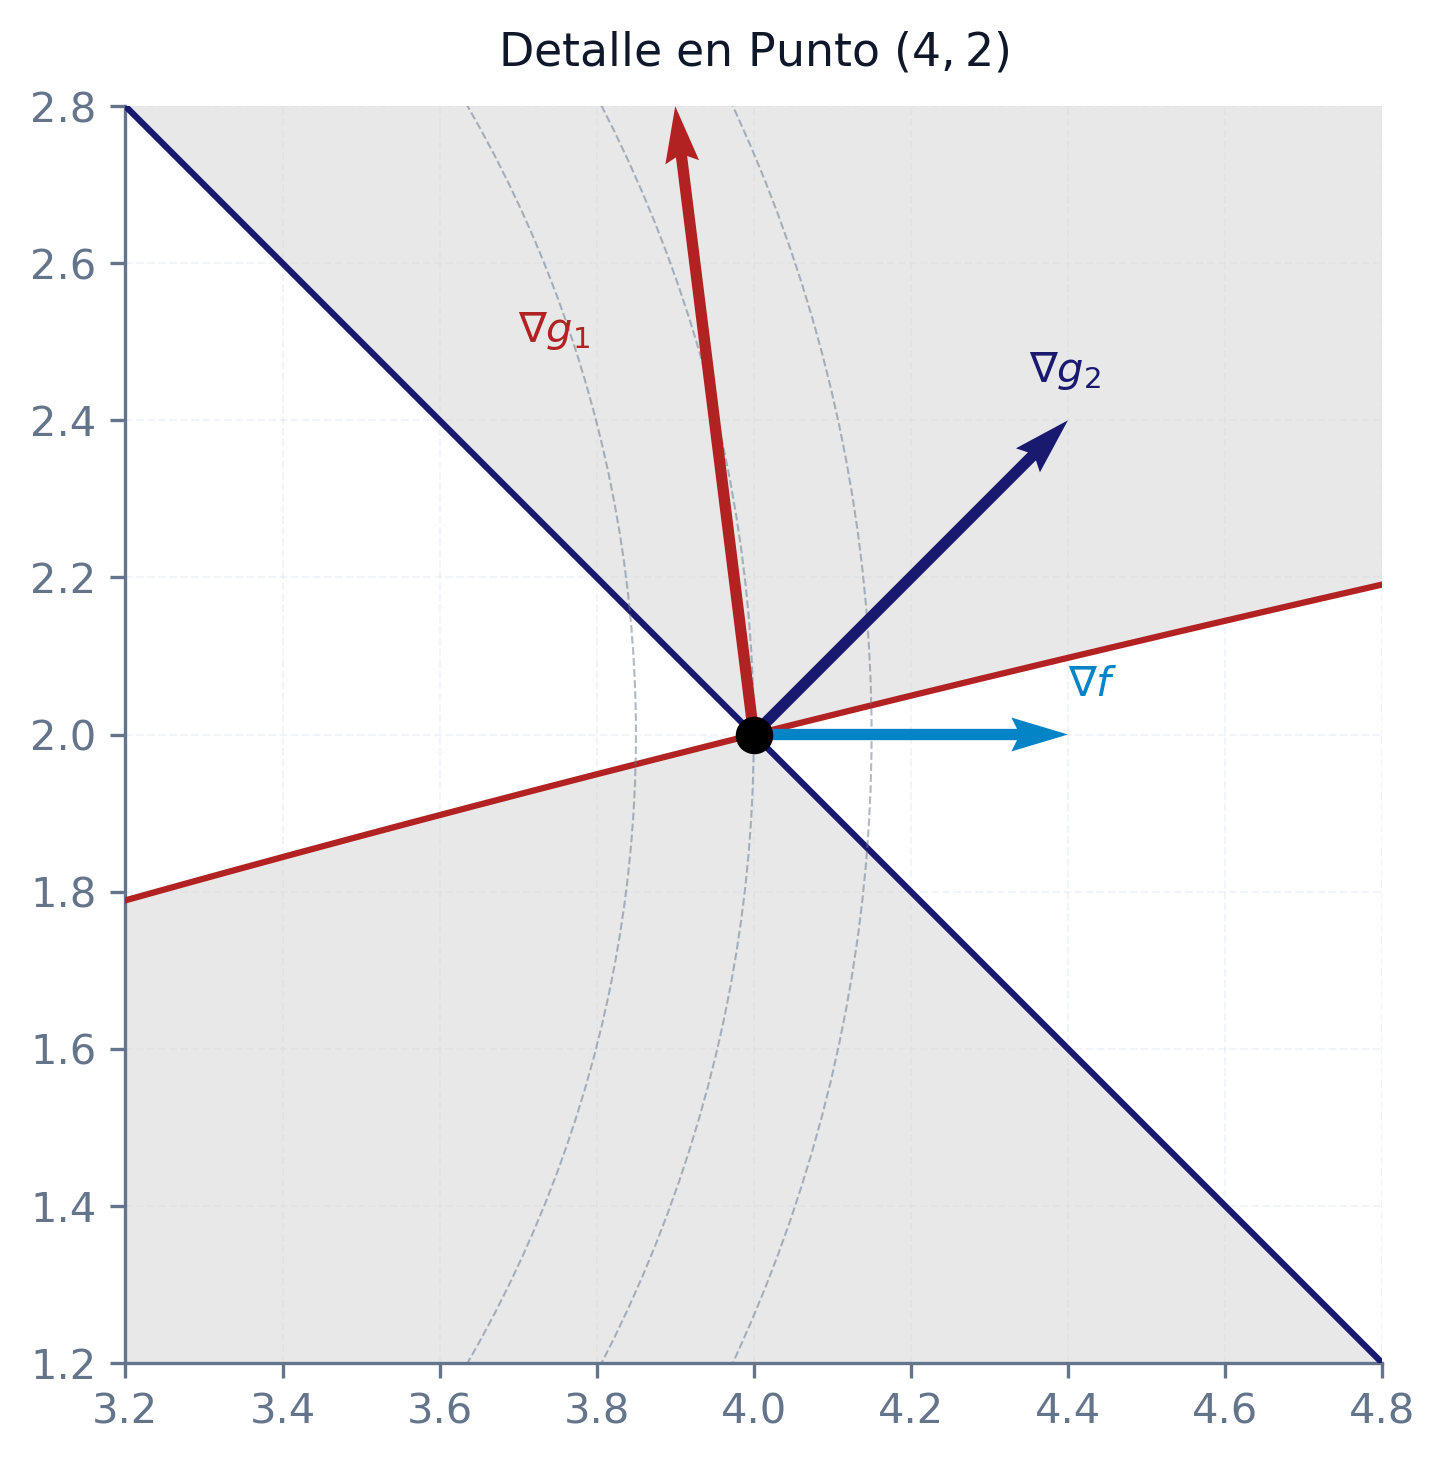
\includegraphics[width=0.6\linewidth,height=\textheight,keepaspectratio]{images/kkt_ejemplo_multiple_zoom_e.png}

    }

    \caption{\label{fig-kkt-ejemplo-multiple-zoom-e}KKT Múltiples
    Restricciones: Detalle en \((4, 2)\)}

    \end{figure}%
  \item
    \emph{Subcaso \(g_2, g_4\) activas
    (\(u_2 \neq 0, u_4 \neq 0, u_1=u_3=0\))}: Gives \(y = 0\) y
    \(x + y = 6 \implies x = 6\). Estacionariedad:
    \[ u_2 = -2(6 - 2.25) = -7.50 < 0 \]
    \[ u_4 = 2(0 - 2) + u_2 = -4 - 7.50 = -11.50 < 0 \] Ambos
    multiplicadores son negativos, por lo que el punto
    \textbf{\((6, 0)\)} es un candidato a máximo local (ver detalle en
    Figura~\ref{fig-kkt-ejemplo-multiple-zoom-c}). Comprobamos
    factibilidad en \(g_1\):
    \[ g_1(6, 0) = -6 + 0 = -6 \le 0 \quad (\text{factible}) \] Por
    tanto, el candidato es válido.

    \begin{figure}[H]

    \centering{

    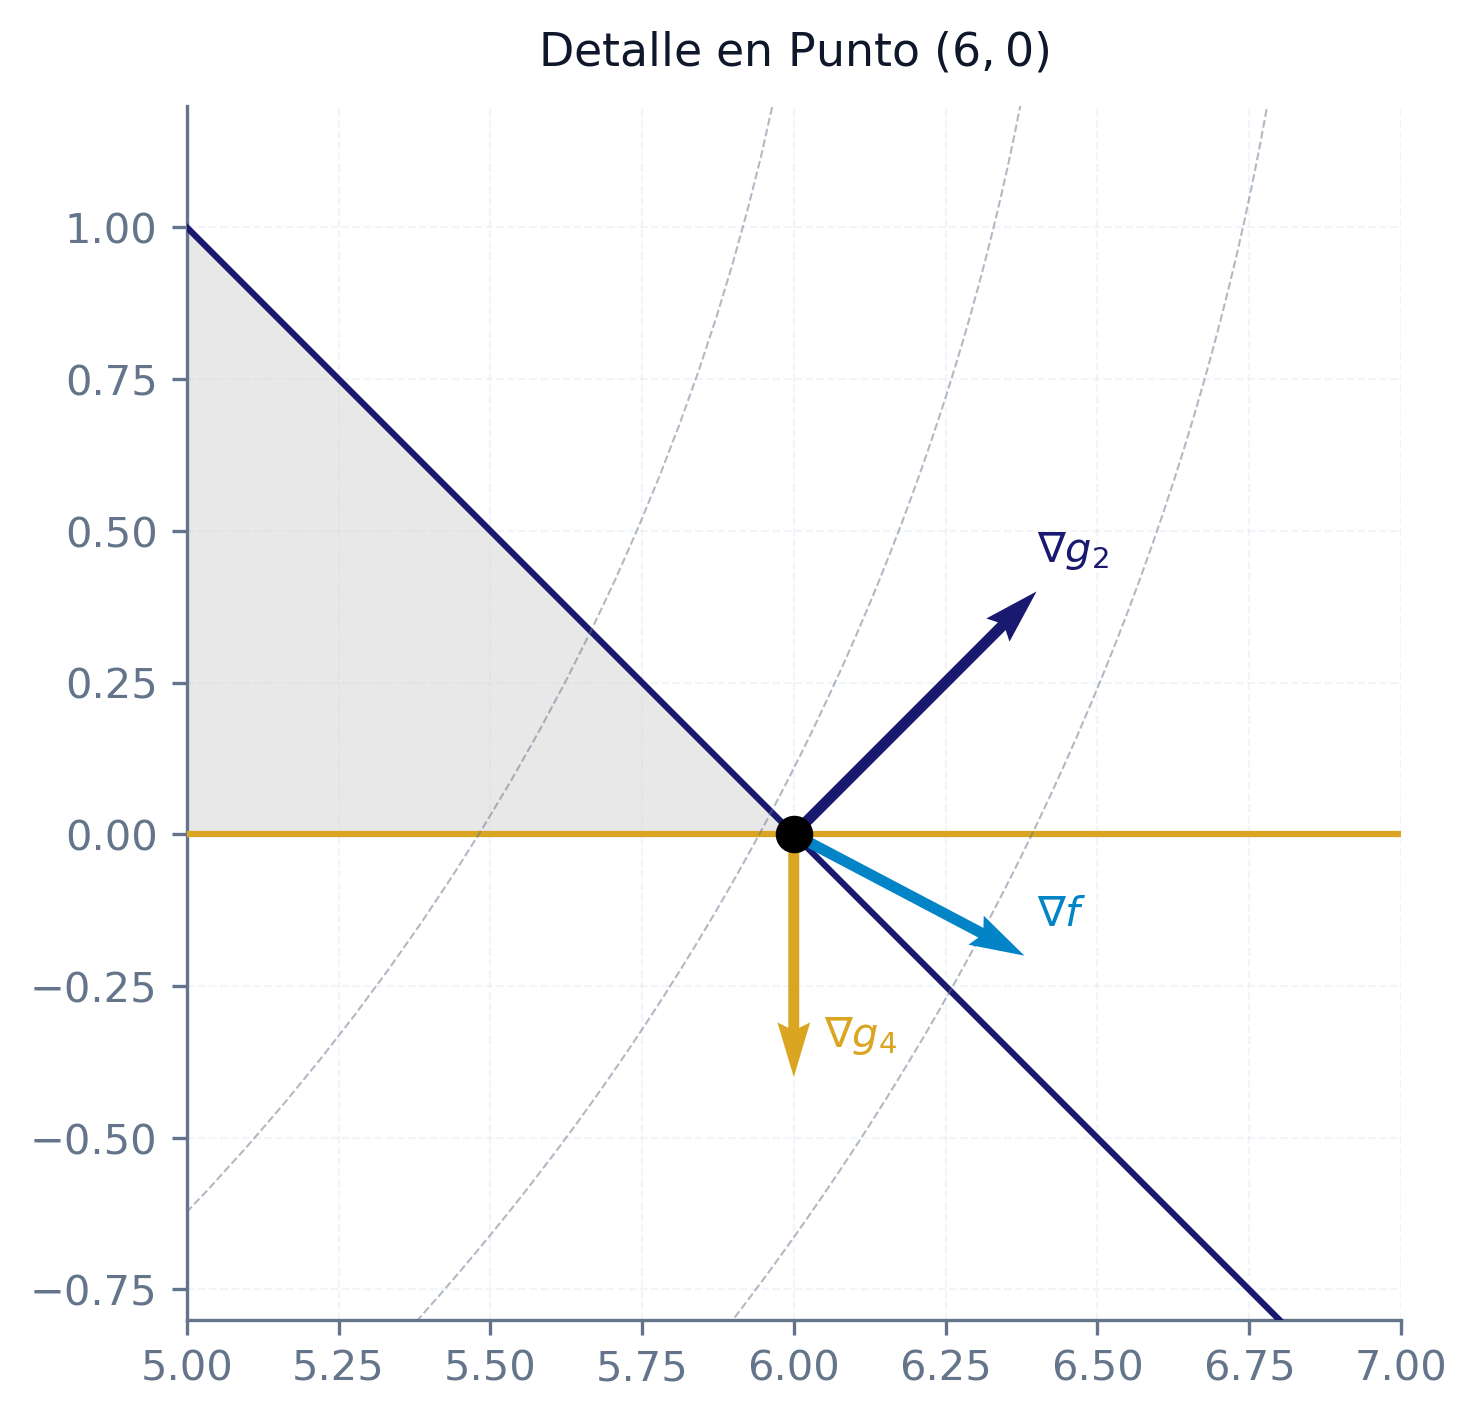
\includegraphics[width=0.6\linewidth,height=\textheight,keepaspectratio]{images/kkt_ejemplo_multiple_zoom_c.png}

    }

    \caption{\label{fig-kkt-ejemplo-multiple-zoom-c}KKT Múltiples
    Restricciones: Detalle en \((6, 0)\)}

    \end{figure}%
  \item
    \emph{Subcaso \(g_3, g_4\) activas
    (\(u_3 \neq 0, u_4 \neq 0, u_1=u_2=0\))}: Gives \(x = 0, y = 0\).
    Estacionariedad: \[ u_3 = 2(0 - 2.25) = -4.50 < 0 \]
    \[ u_4 = 2(0 - 2) = -4.00 < 0 \] Ambos multiplicadores son
    negativos, por lo que el punto \textbf{\((0, 0)\)} es candidato a
    máximo (ver detalle en
    Figura~\ref{fig-kkt-ejemplo-multiple-zoom-b}). Sin embargo, en
    \((0,0)\) la restricción \(g_1(0,0) = 0\) también es activa, lo que
    significa que hay tres restricciones activas y los gradientes
    correspondientes son linealmente dependientes (fallo de LICQ). No es
    un punto KKT regular, pero es un punto Fritz-John con \(u_0=0\)
    (candidato a máximo).

    \begin{figure}[H]

    \centering{

    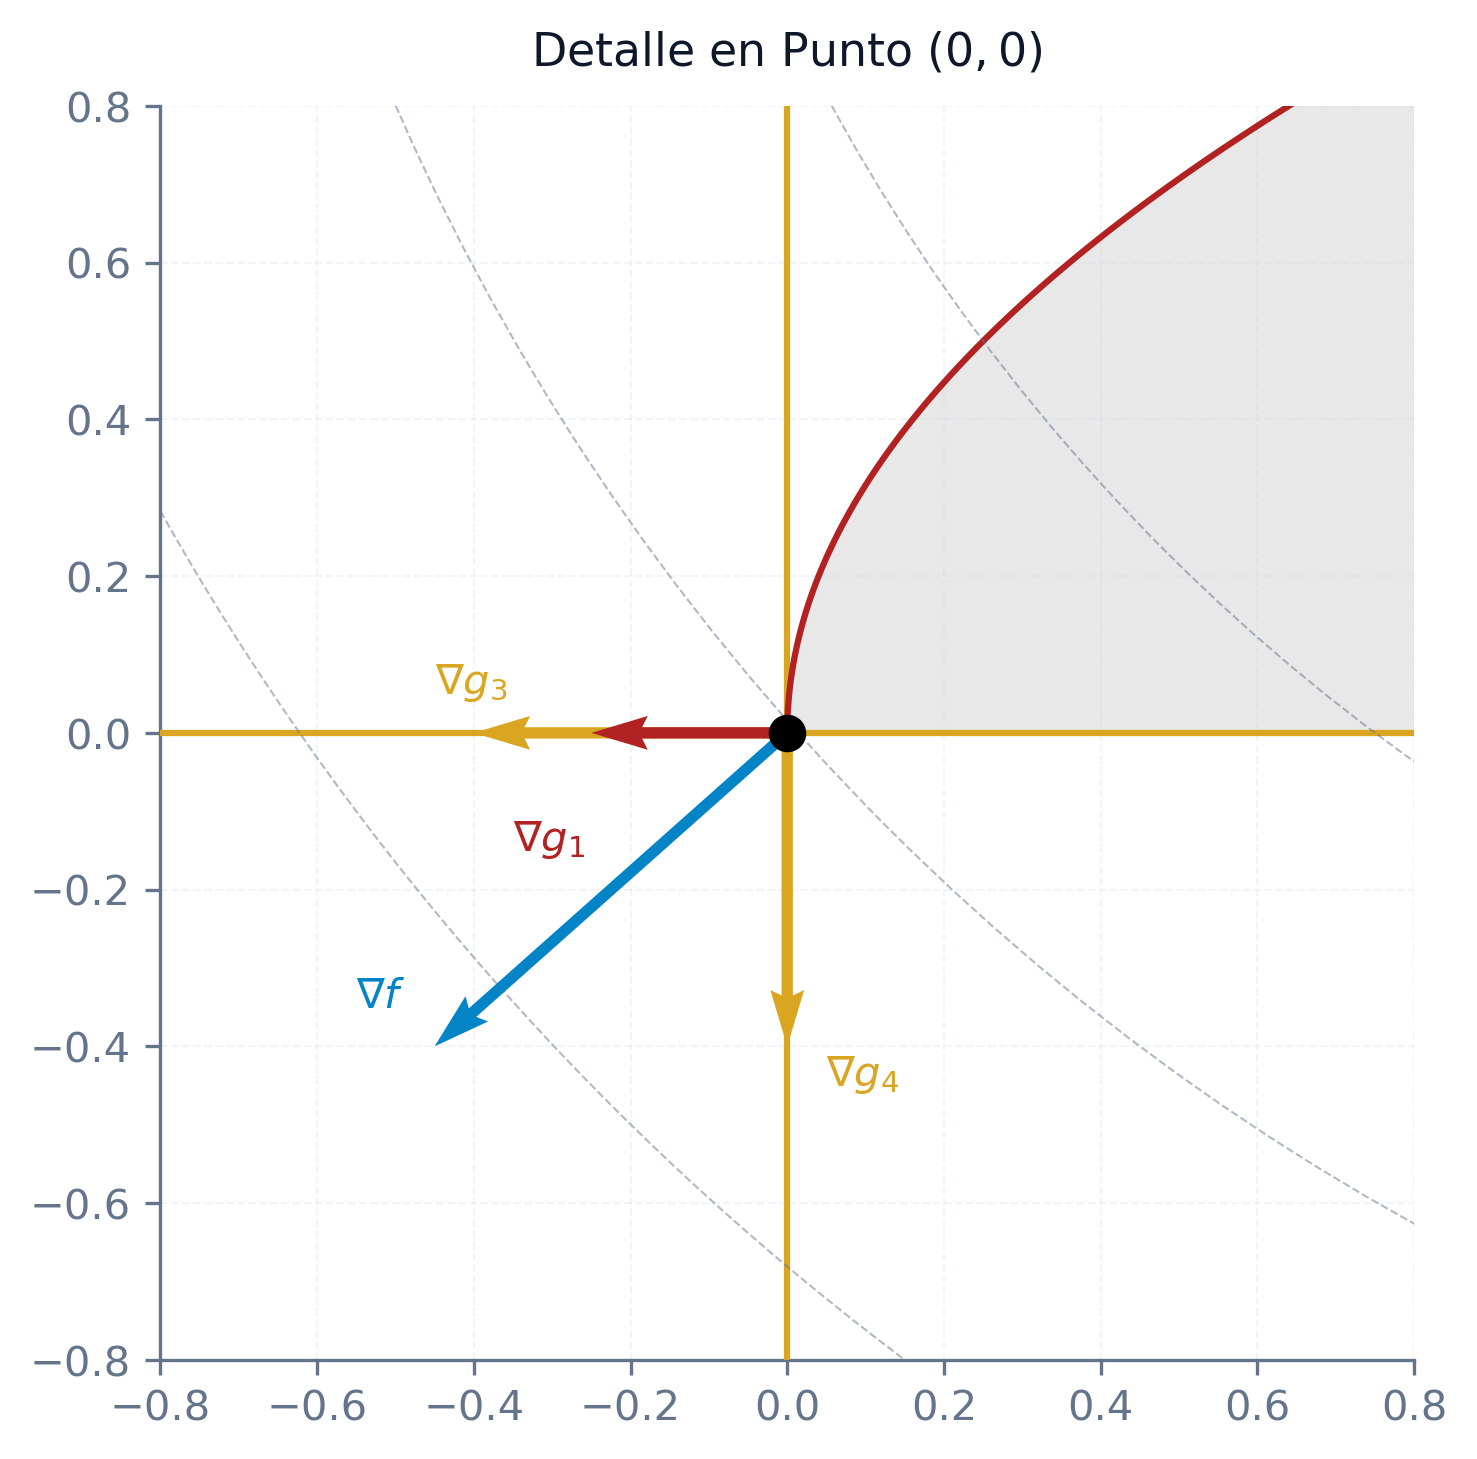
\includegraphics[width=0.6\linewidth,height=\textheight,keepaspectratio]{images/kkt_ejemplo_multiple_zoom_b.png}

    }

    \caption{\label{fig-kkt-ejemplo-multiple-zoom-b}KKT Múltiples
    Restricciones: Detalle en \((0, 0)\)}

    \end{figure}%
  \end{itemize}
\end{itemize}

\textbf{Conclusión y Caracterización de Candidatos}

Al evaluar las condiciones suficientes y comparar los valores de la
función objetivo:

\begin{itemize}
\tightlist
\item
  \textbf{Mínimos}: El único candidato KKT es \textbf{\((2.40, 1.55)\)}
  con \(f(2.40, 1.55) \approx 0.22\).

  \begin{itemize}
  \tightlist
  \item
    La función objetivo \(f\) es cuadrática estrictamente convexa.
  \item
    La restricción activa \(g_1(x, y) = -x + y^2\) es convexa en todo su
    dominio (su Hessiana
    \(H_1 = \begin{pmatrix} 0 & 0 \\ 0 & 2 \end{pmatrix} \succeq 0\) es
    semidefinida positiva).
  \item
    Al ser \(f\) convexa y la restricción activa convexa con
    multiplicador positivo, se satisfacen las condiciones suficientes,
    confirmando que \textbf{\((2.40, 1.55)\) es el mínimo global}.
  \end{itemize}
\item
  \textbf{Máximos}: Evaluamos los candidatos a máximo (\(u_i \le 0\)):

  \begin{itemize}
  \tightlist
  \item
    \((6,0) \implies f(6,0) = 18.06\) (Máximo global).
  \item
    \((0,0) \implies f(0,0) \approx 9.06\) (Máximo local, verificado
    como punto singular).
  \item
    \((2.25, 0) \implies f(2.25,0) = 4.00\) (No verifica las condiciones
    suficientes).
  \end{itemize}
\end{itemize}

En la Figura~\ref{fig-kkt-ejemplo-multiple-conclusiones} se resume
gráficamente el resultado de la caracterización y la condición de cada
uno de los cinco candidatos estudiados.

\begin{figure}[H]

\centering{

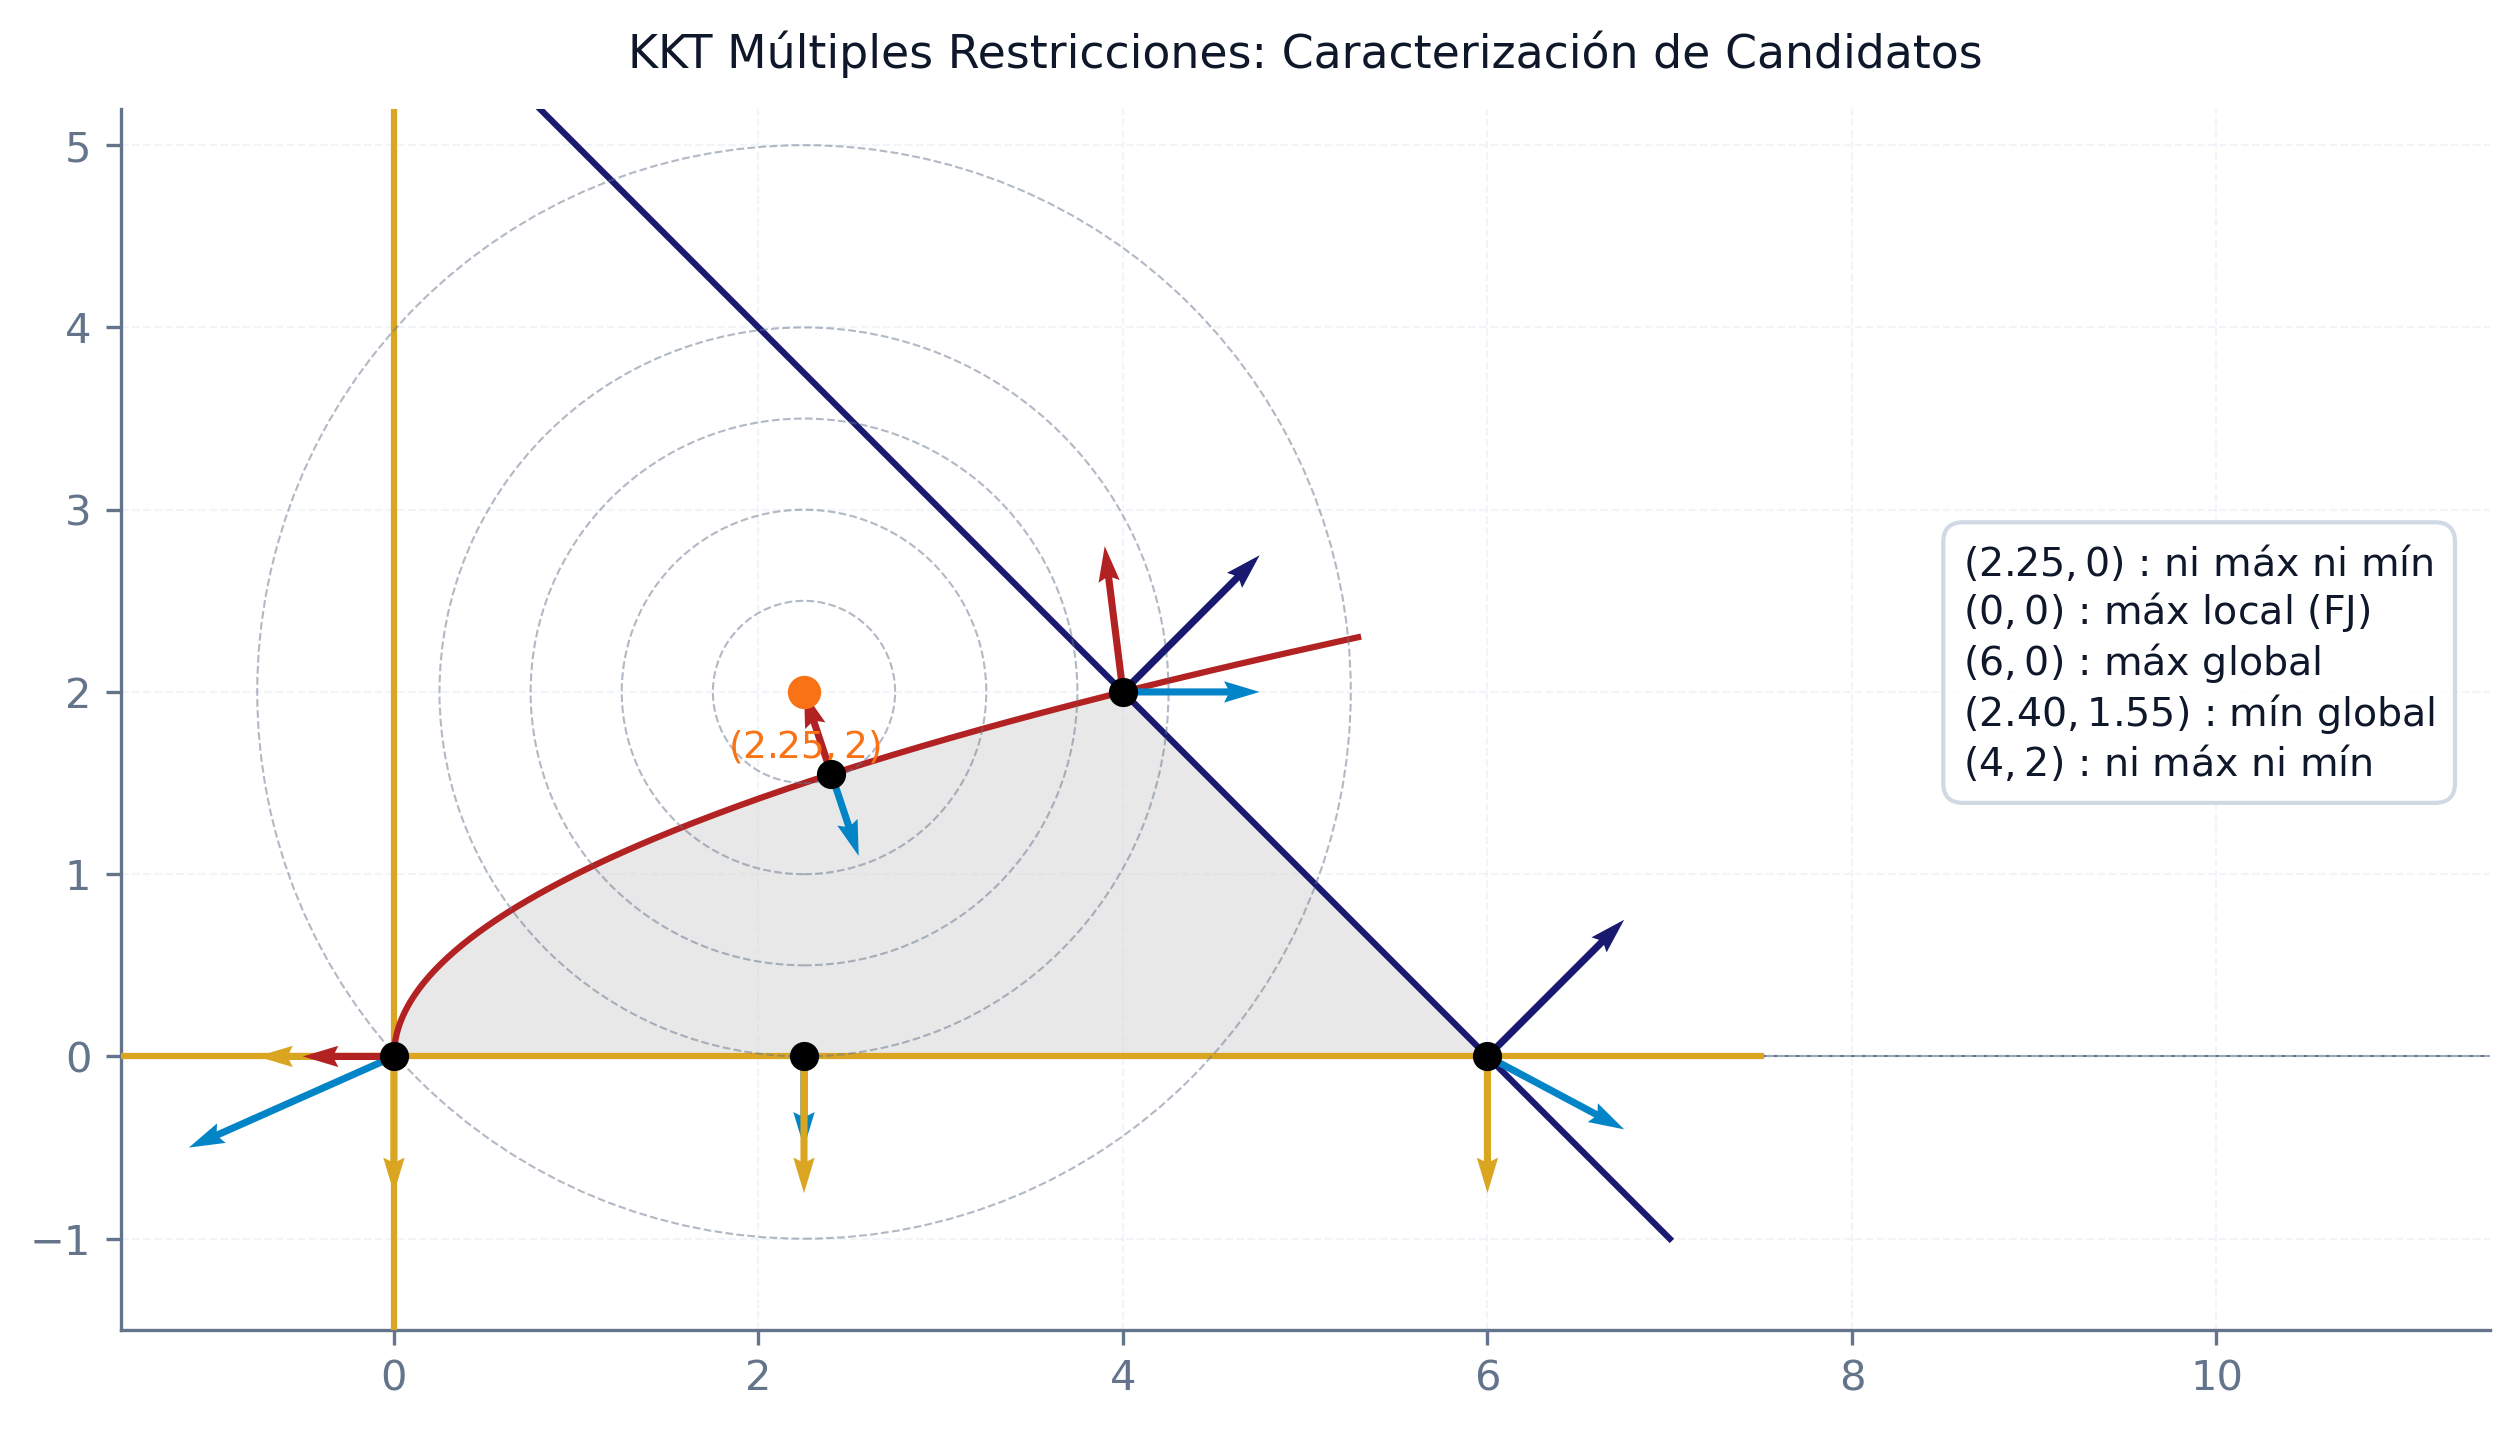
\includegraphics[width=0.75\linewidth,height=\textheight,keepaspectratio]{images/kkt_ejemplo_multiple_desigualdad_conclusiones.png}

}

\caption{\label{fig-kkt-ejemplo-multiple-conclusiones}KKT Múltiples
Restricciones: Caracterización de Candidatos}

\end{figure}%

\end{tcolorbox}

\begin{tcolorbox}[enhanced jigsaw, toprule=.15mm, opacitybacktitle=0.6, coltitle=black, colbacktitle=quarto-callout-tip-color!10!white, title=\textcolor{quarto-callout-tip-color}{\faLightbulb}\hspace{0.5em}{Ejemplo: Optimización con restricción circular y lineal}, arc=.35mm, rightrule=.15mm, toptitle=1mm, breakable, bottomtitle=1mm, titlerule=0mm, colback=white, opacityback=0, leftrule=.75mm, colframe=quarto-callout-tip-color-frame, left=2mm, bottomrule=.15mm]

Consideremos el problema de encontrar los mínimos y máximos locales y
globales de: \[
\begin{aligned}
\min/\max \quad & f(x, y) = 3x - y \\
\text{s.a.} \quad & g_1(x, y) = x^2 + y^2 - 1 \le 0 \\
& g_2(x, y) = -4x - y + 1 \le 0
\end{aligned}
\]

El gradiente de la función objetivo y de las restricciones son: \[
\nabla f = \begin{pmatrix} 3 \\ -1 \end{pmatrix}, \quad \nabla g_1 = \begin{pmatrix} 2x \\ 2y \end{pmatrix}, \quad \nabla g_2 = \begin{pmatrix} -4 \\ -1 \end{pmatrix}
\]

La función Lagrangiana es:
\[ L(x, y, u) = 3x - y + u_1(x^2 + y^2 - 1) + u_2(-4x - y + 1) \]

El sistema de condiciones KKT se plantea como:

\begin{enumerate}
\def\labelenumi{\arabic{enumi}.}
\tightlist
\item
  \textbf{Estacionariedad (Factibilidad dual)}:
  \[ \frac{\partial L}{\partial x} = 3 + 2x u_1 - 4u_2 = 0 \]
  \[ \frac{\partial L}{\partial y} = -1 + 2y u_1 - u_2 = 0 \]
\item
  \textbf{Factibilidad primal}:
  \[ x^2 + y^2 - 1 \le 0, \quad -4x - y + 1 \le 0 \]
\item
  \textbf{Ortogonalidad (Holgura complementaria)}:
  \[ u_1(x^2 + y^2 - 1) = 0, \quad u_2(-4x - y + 1) = 0 \]
\item
  \textbf{Signo de los multiplicadores}:

  \begin{itemize}
  \tightlist
  \item
    Para \textbf{mínimos}: \(u_i \ge 0, \ \forall i = 1, 2\).
  \item
    Para \textbf{máximos}: \(u_i \le 0, \ \forall i = 1, 2\).
  \end{itemize}
\end{enumerate}

Geométricamente, el problema representa la minimización o maximización
de la función lineal \(3x - y\) sobre una región factible
\(\mathcal{S}\) acotada por la circunferencia unitaria y la recta
\(4x+y \ge 1\) (ver Figura~\ref{fig-kkt-ejemplo-circ-lineal-general}).

\begin{figure}[H]

\centering{

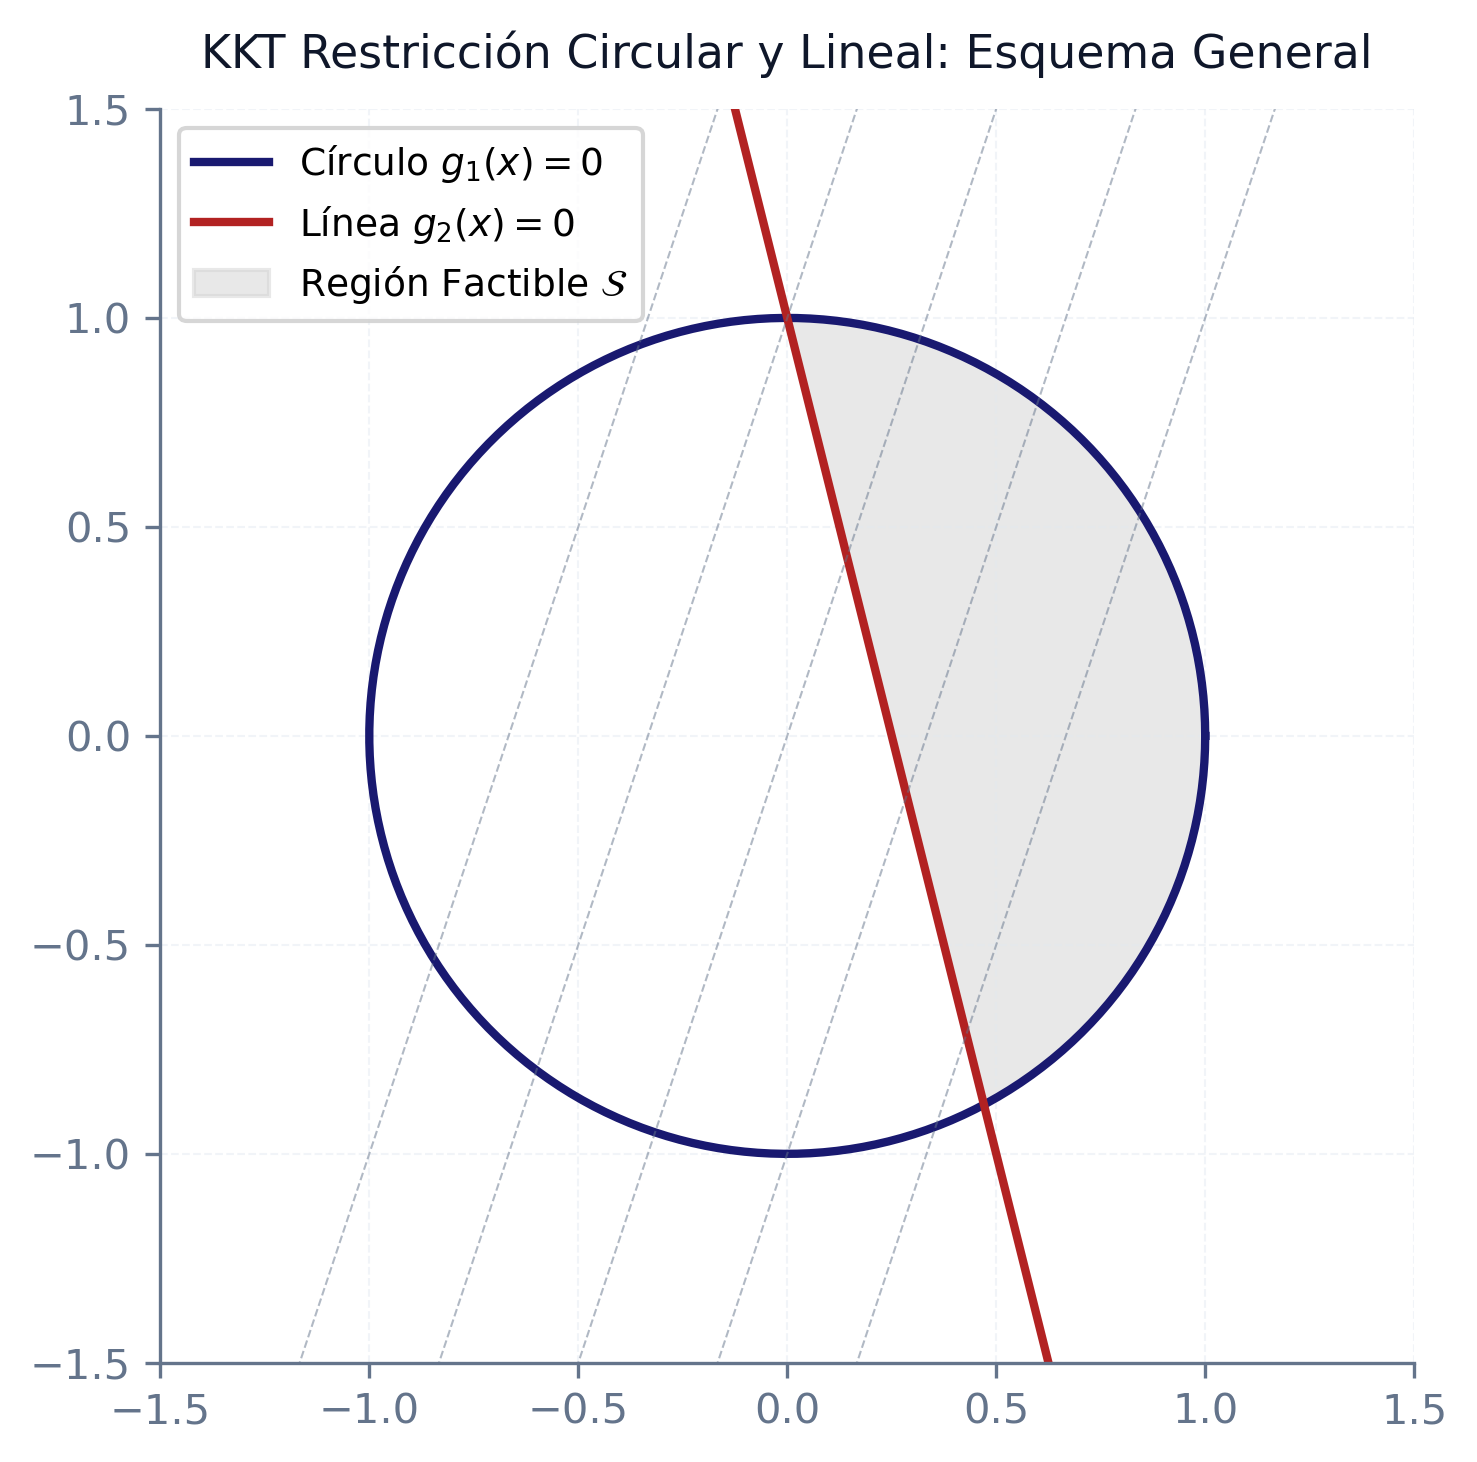
\includegraphics[width=0.6\linewidth,height=\textheight,keepaspectratio]{images/kkt_ejemplo_circ_lineal_general.png}

}

\caption{\label{fig-kkt-ejemplo-circ-lineal-general}KKT Restricción
Circular y Lineal: Esquema General}

\end{figure}%

\textbf{Resolución combinatoria por casos}

Analizamos las combinaciones de restricciones activas e inactivas
mediante la holgura complementaria:

\begin{itemize}
\item
  \textbf{Caso 1: Ambas restricciones inactivas (\(u_1 = 0, u_2 = 0\))}:
  De las ecuaciones de estacionariedad obtenemos:
  \[ 3 = 0 \qquad \text{y} \qquad -1 = 0 \] lo cual representa una
  contradicción inmediata. Por lo tanto, no existen puntos estacionarios
  en el interior de la región factible.
\item
  \textbf{Caso 2: Una única restricción activa}:

  \begin{itemize}
  \item
    \emph{Subcaso \(g_1\) activa (\(u_1 \neq 0, u_2 = 0\))}: El sistema
    de estacionariedad se reduce a:
    \[ 3 + 2x u_1 = 0 \implies x = -\frac{3}{2u_1} \]
    \[ -1 + 2y u_1 = 0 \implies y = \frac{1}{2u_1} \] Como \(g_1\) es
    activa, se cumple \(x^2 + y^2 = 1\). Sustituyendo las expresiones en
    la ecuación de la circunferencia:
    \[ \left(-\frac{3}{2u_1}\right)^2 + \left(\frac{1}{2u_1}\right)^2 = 1 \implies \frac{9}{4u_1^2} + \frac{1}{4u_1^2} = 1 \implies \frac{10}{4u_1^2} = 1 \implies u_1^2 = \frac{10}{4}\]
    \[\implies u_1 = \pm \frac{\sqrt{10}}{2} \]

    Analizamos las dos posibles soluciones para \(u_1\):

    \begin{enumerate}
    \def\labelenumi{\arabic{enumi}.}
    \item
      \textbf{Si \(u_1 = \frac{\sqrt{10}}{2} \approx 1.58 > 0\)
      (candidato a mínimo)}: Obtenemos las coordenadas del punto:
      \[ x = -\frac{3}{\sqrt{10}} \approx -0.95, \qquad y = \frac{1}{\sqrt{10}} \approx 0.32 \]
      Comprobamos la factibilidad primal en la restricción inactiva
      \(g_2\): \[ g_2(-0.95, 0.32) = -4(-0.95) - 0.32 + 1 \]
      \[ = 3.8 - 0.32 + 1 = 4.48 > 0 \quad (\text{no factible}) \] Al
      violar la restricción lineal, este punto se descarta (ver detalle
      en Figura~\ref{fig-kkt-ejemplo-circ-lineal-zoom-a}).

      \begin{figure}[H]

      \centering{

      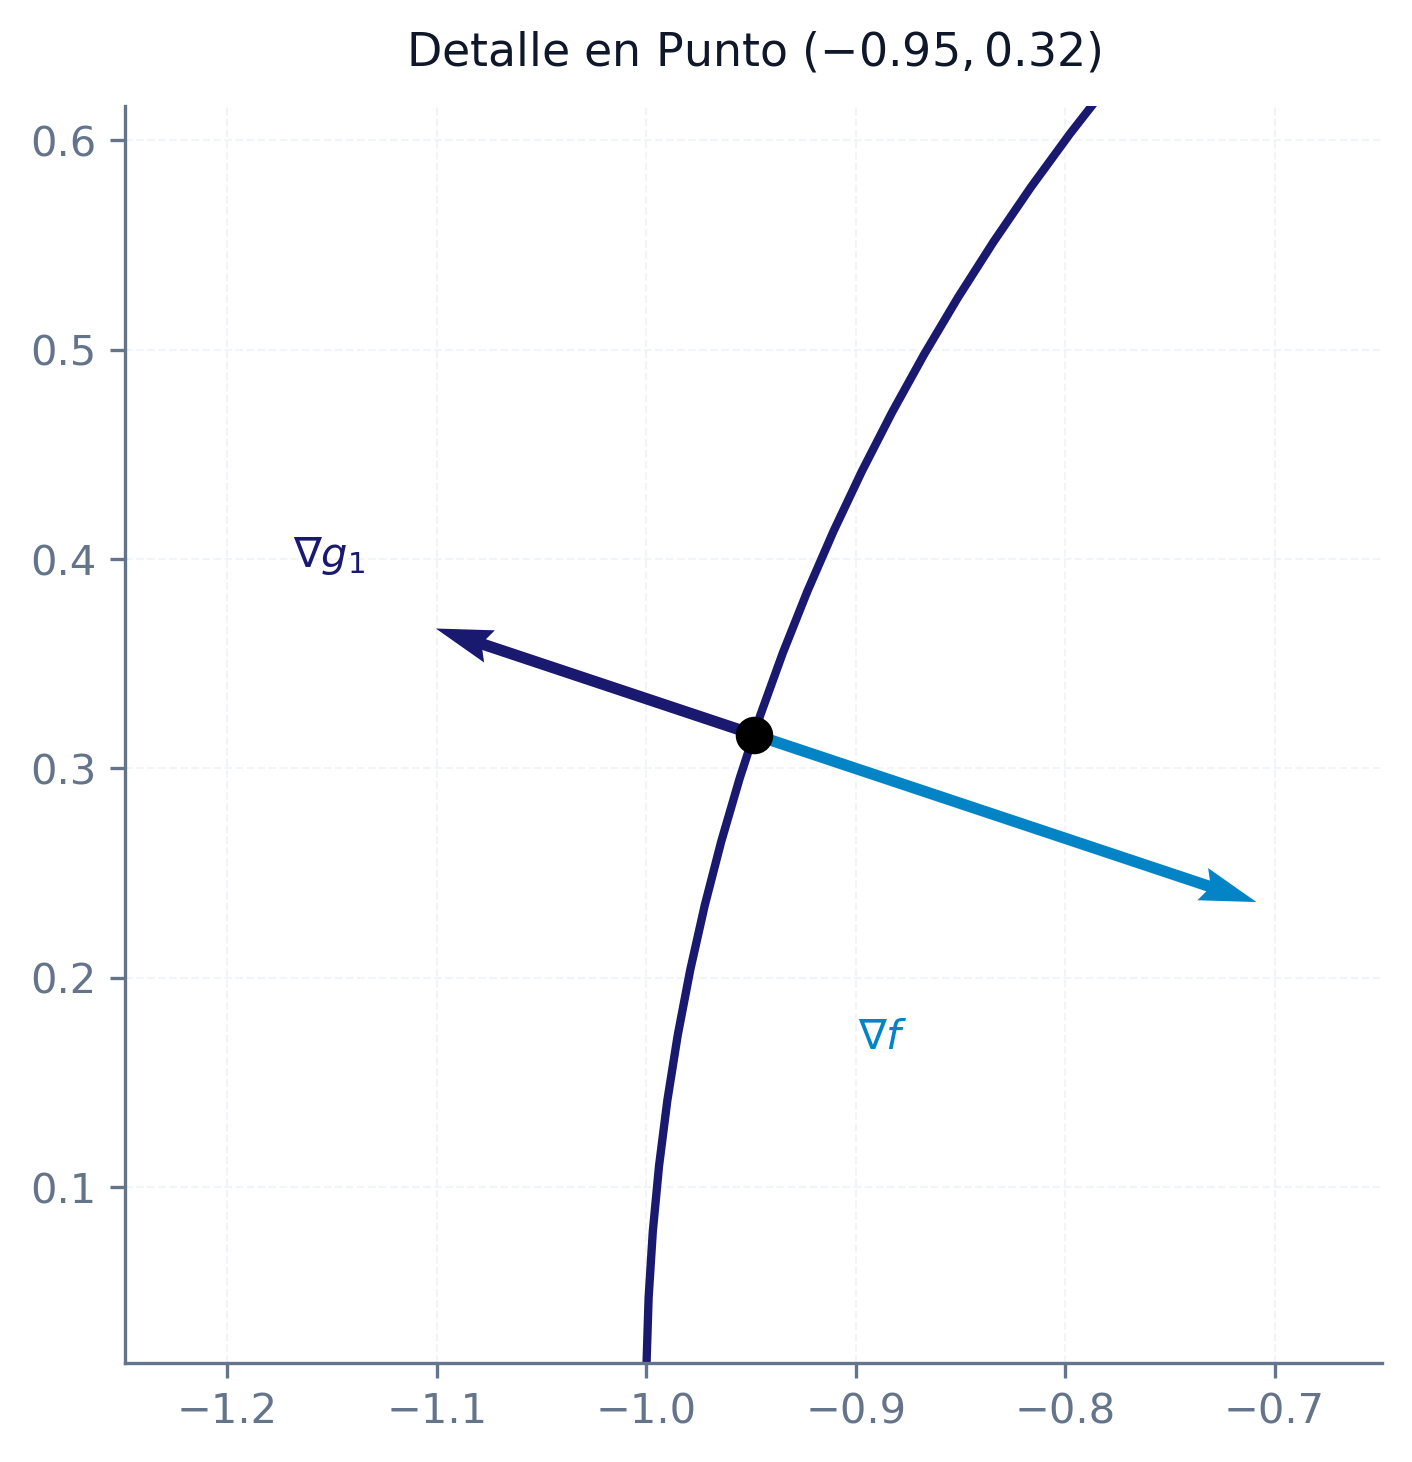
\includegraphics[width=0.6\linewidth,height=\textheight,keepaspectratio]{images/kkt_ejemplo_circ_lineal_zoom_a.png}

      }

      \caption{\label{fig-kkt-ejemplo-circ-lineal-zoom-a}KKT Restricción
      Circular y Lineal: Detalle en \((-0.95, 0.32)\)}

      \end{figure}%
    \item
      \textbf{Si \(u_1 = -\frac{\sqrt{10}}{2} \approx -1.58 < 0\)
      (candidato a máximo)}: Obtenemos las coordenadas del punto:
      \[ x = \frac{3}{\sqrt{10}} \approx 0.95, \qquad y = -\frac{1}{\sqrt{10}} \approx -0.32 \]
      Comprobamos la factibilidad primal en la restricción inactiva
      \(g_2\): \[ g_2(0.95, -0.32) = -4(0.95) - (-0.32) + 1 = \]
      \[-3.8 + 0.32 + 1 = -2.48 \le 0 \quad (\text{factible}) \] Como es
      factible y \(u_1 < 0\) (con \(u_2 = 0\)), el punto
      \textbf{\(\left(\frac{3}{\sqrt{10}}, -\frac{1}{\sqrt{10}}\right)\)}
      es un candidato válido a máximo local (ver detalle en
      Figura~\ref{fig-kkt-ejemplo-circ-lineal-zoom-b}).

      \begin{figure}[H]

      \centering{

      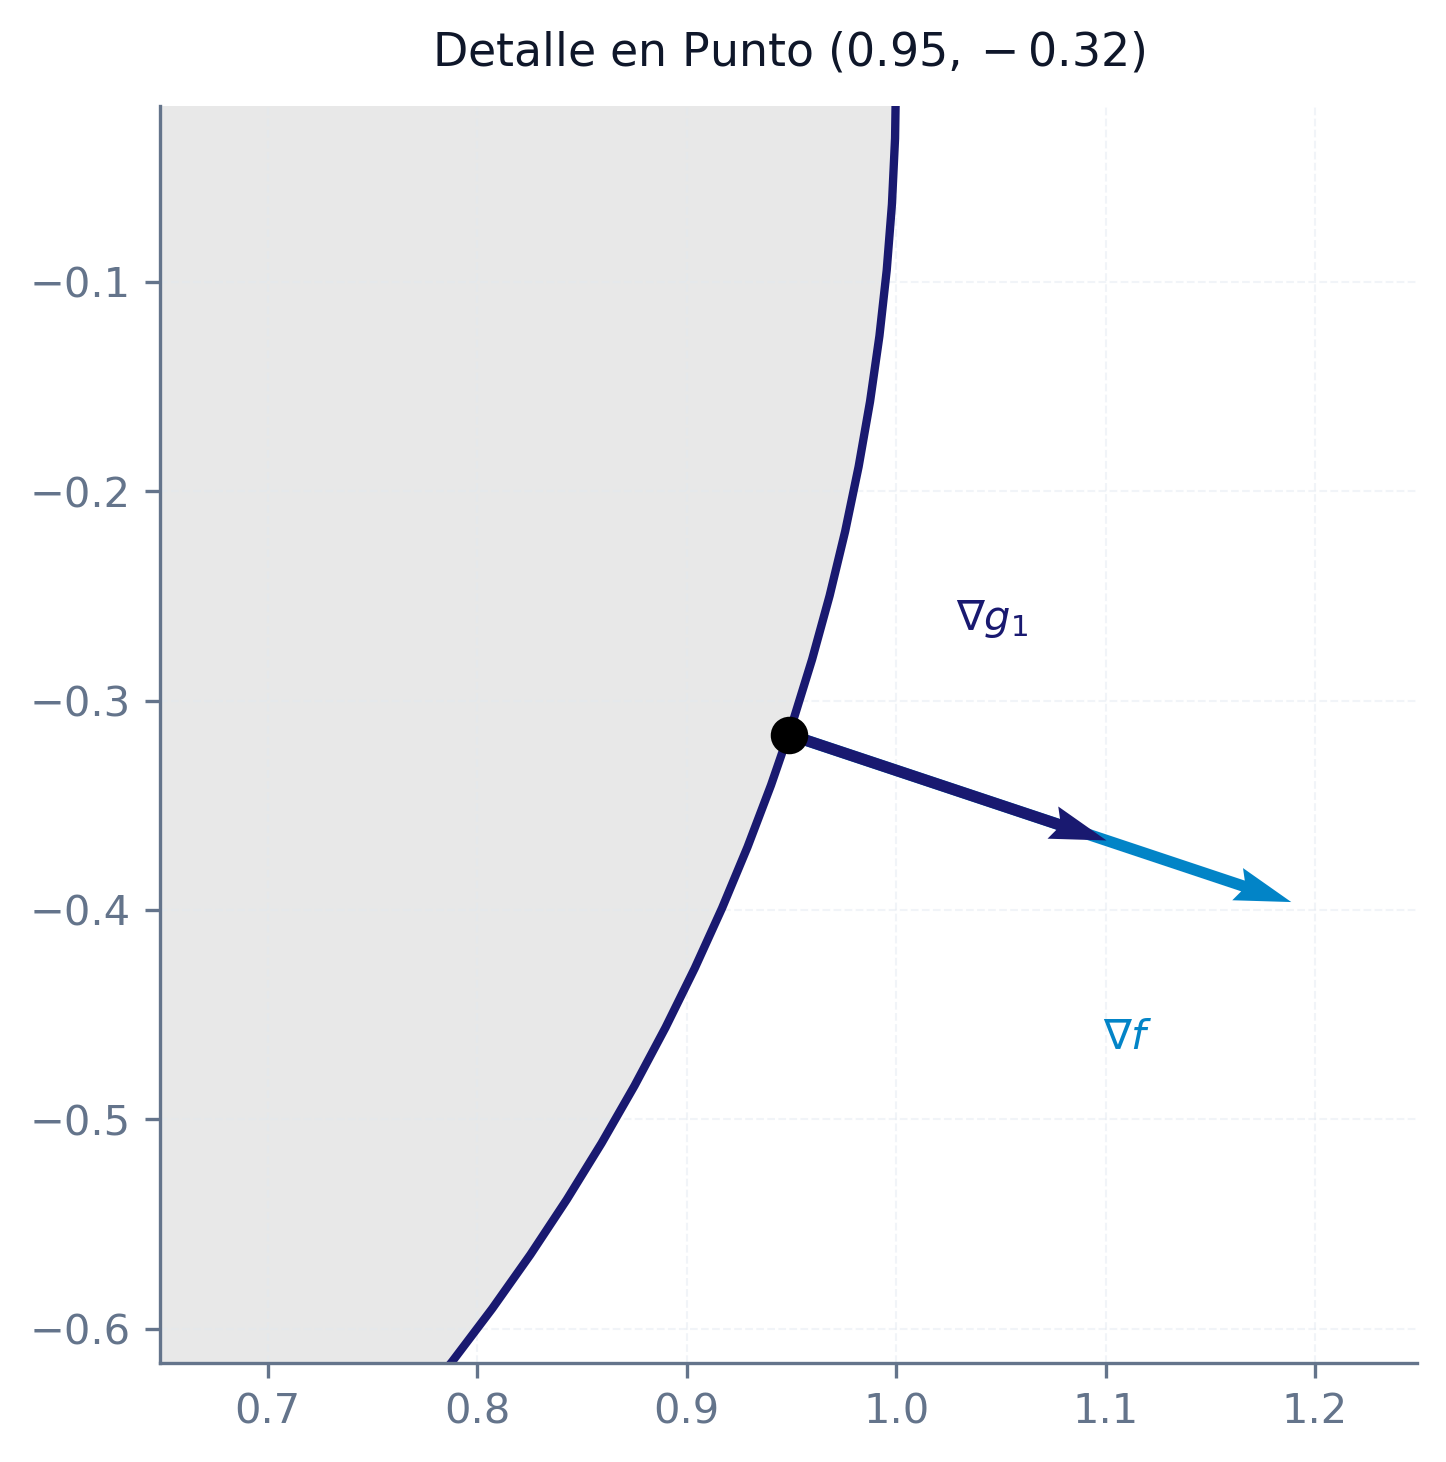
\includegraphics[width=0.6\linewidth,height=\textheight,keepaspectratio]{images/kkt_ejemplo_circ_lineal_zoom_b.png}

      }

      \caption{\label{fig-kkt-ejemplo-circ-lineal-zoom-b}KKT Restricción
      Circular y Lineal: Detalle en \((0.95, -0.32)\)}

      \end{figure}%
    \end{enumerate}
  \item
    \emph{Subcaso \(g_2\) activa (\(u_2 \neq 0, u_1 = 0\))}: El sistema
    de estacionariedad se reduce a:
    \[ 3 - 4u_2 = 0 \implies u_2 = \frac{3}{4} = 0.75 \]
    \[ -1 - u_2 = 0 \implies u_2 = -1 \] Lo cual es una contradicción
    (\(0.75 \neq -1\)). Por lo tanto, no existen candidatos con
    únicamente la restricción lineal activa.
  \end{itemize}
\item
  \textbf{Caso 3: Ambas restricciones activas
  (\(u_1 \neq 0, u_2 \neq 0\))}: Los puntos de intersección de la
  circunferencia y la recta satisfacen \(x^2 + y^2 = 1\) y
  \(-4x - y + 1 = 0 \implies y = 1 - 4x\). Sustituyendo \(y\) en la
  circunferencia:
  \[ x^2 + (1 - 4x)^2 = 1 \implies x^2 + 1 - 8x + 16x^2 = 1 \implies 17x^2 - 8x = 0 \]
  Esto nos da las soluciones:

  \begin{enumerate}
  \def\labelenumi{\arabic{enumi}.}
  \tightlist
  \item
    \(x = 0 \implies y = 1\).
  \item
    \(x = 8/17 \approx 0.47 \implies y = -15/17 \approx -0.88\).
  \end{enumerate}

  Evaluamos los multiplicadores para cada uno de estos dos puntos de
  intersección:

  \begin{itemize}
  \item
    \emph{Punto \((0, 1)\)}: Sustituyendo en el sistema de
    estacionariedad:
    \[ 3 + 2(0)u_1 - 4u_2 = 0 \implies 3 - 4u_2 = 0 \implies u_2 = \frac{3}{4} \ge 0 \]
    \[ -1 + 2(1)u_1 - u_2 = 0 \implies 2u_1 = 1 + u_2 = 1 + \frac{3}{4} = \frac{7}{4} \implies u_1 = \frac{7}{8} \ge 0 \]
    Como ambos multiplicadores son no negativos
    (\(u_1 = 7/8 \ge 0, \ u_2 = 3/4 \ge 0\)), el punto
    \textbf{\((0, 1)\)} es un candidato a mínimo local (ver detalle en
    Figura~\ref{fig-kkt-ejemplo-circ-lineal-zoom-c}).

    \begin{figure}[H]

    \centering{

    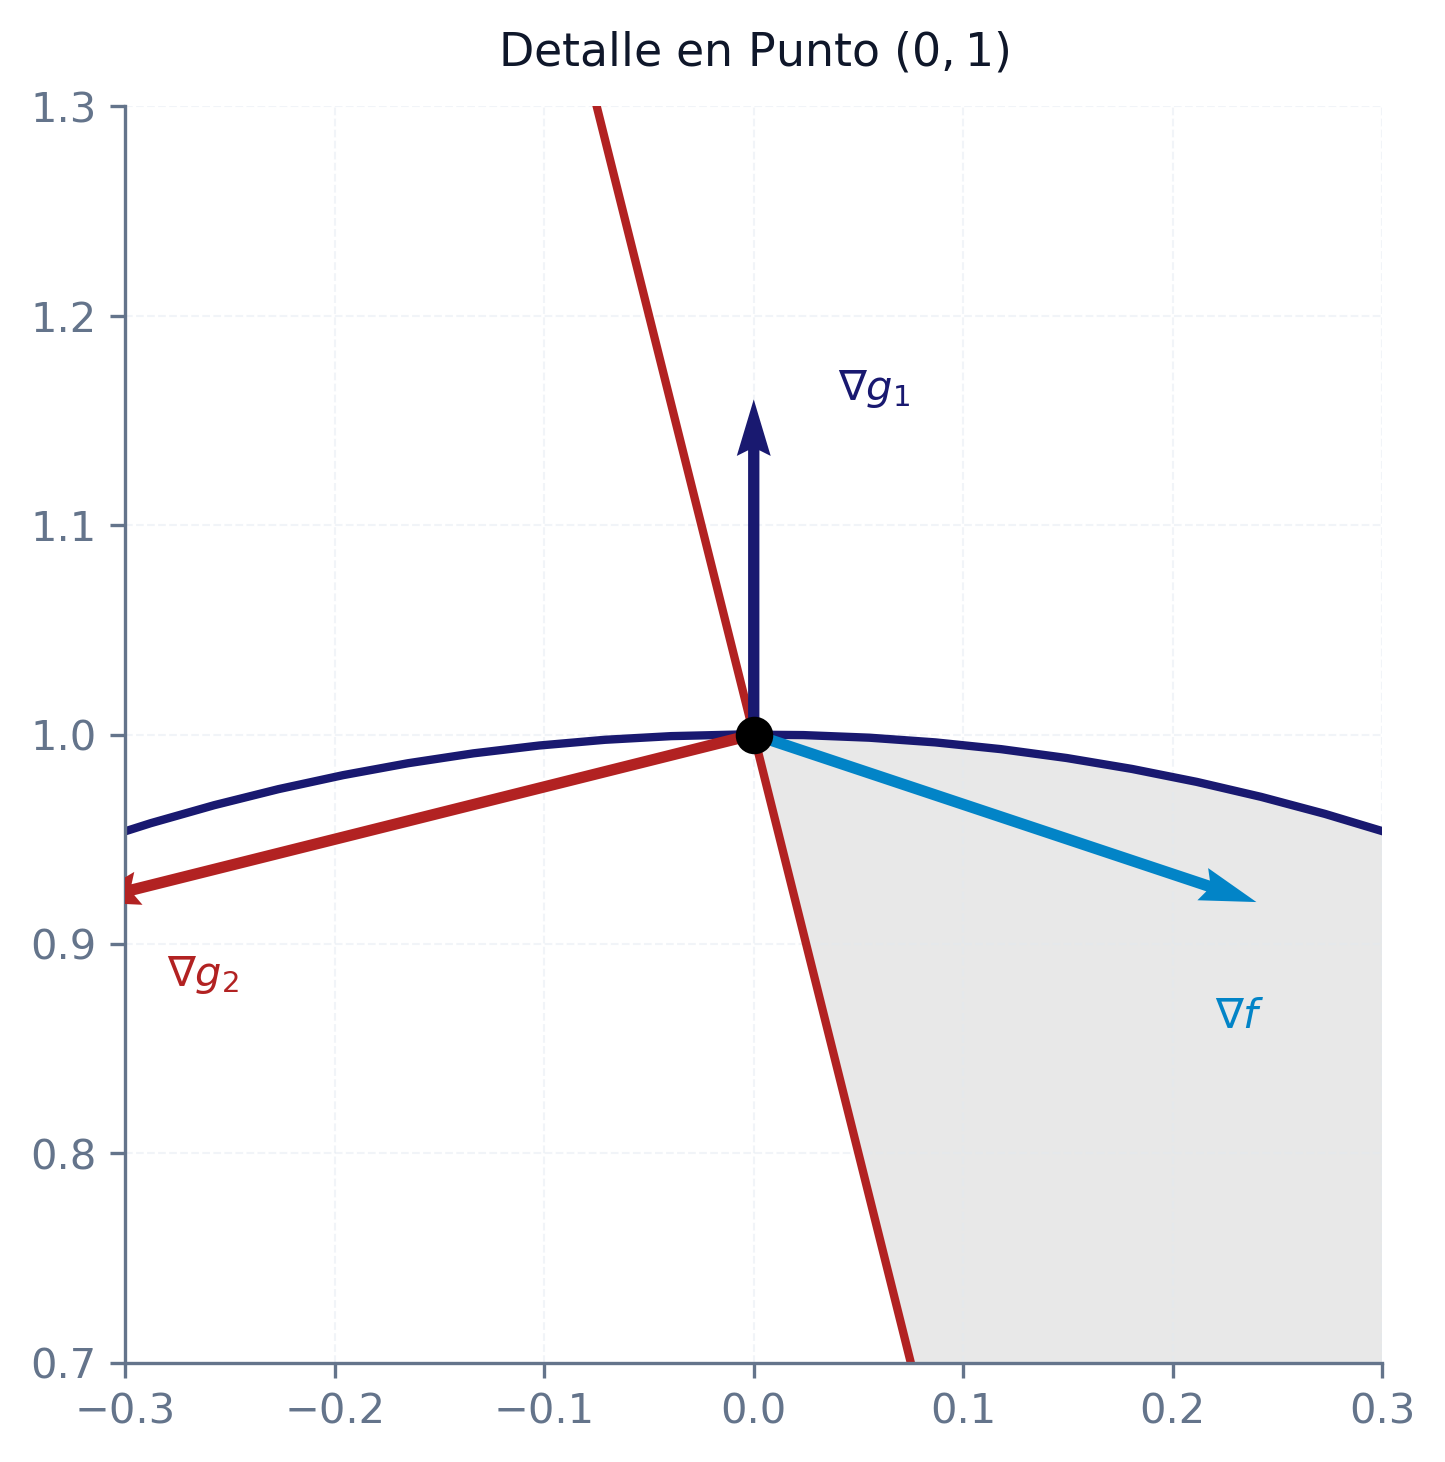
\includegraphics[width=0.6\linewidth,height=\textheight,keepaspectratio]{images/kkt_ejemplo_circ_lineal_zoom_c.png}

    }

    \caption{\label{fig-kkt-ejemplo-circ-lineal-zoom-c}KKT Restricción
    Circular y Lineal: Detalle en \((0, 1)\)}

    \end{figure}%
  \item
    \emph{Punto \((8/17, -15/17)\)}: Sustituyendo en el sistema de
    estacionariedad: \[ 3 + \frac{16}{17} u_1 - 4u_2 = 0 \]
    \[ -1 - \frac{30}{17} u_1 - u_2 = 0 \implies u_2 = -1 - \frac{30}{17} u_1 \]
    Sustituyendo la segunda en la primera:
    \[ 3 + \frac{16}{17} u_1 - 4\left(-1 - \frac{30}{17} u_1\right) = 0 \implies 7 + \frac{136}{17} u_1 = 0 \implies 7 + 8u_1 = 0 \implies\]
    \[u_1 = -\frac{7}{8} \approx -0.88 \] Calculamos \(u_2\):
    \[ u_2 = -1 - \frac{30}{17} \left(-\frac{7}{8}\right) = -1 + \frac{105}{68} = \frac{37}{68} \approx 0.54 \]
    Dado que los multiplicadores tienen signos opuestos
    (\(u_1 = -7/8 < 0\) y \(u_2 = 37/68 > 0\)), el punto
    \((8/17, -15/17)\) no cumple los requisitos de signos para ser
    candidato a mínimo ni a máximo (no es punto KKT de primer orden, ver
    detalle en Figura~\ref{fig-kkt-ejemplo-circ-lineal-zoom-d}).

    \begin{figure}[H]

    \centering{

    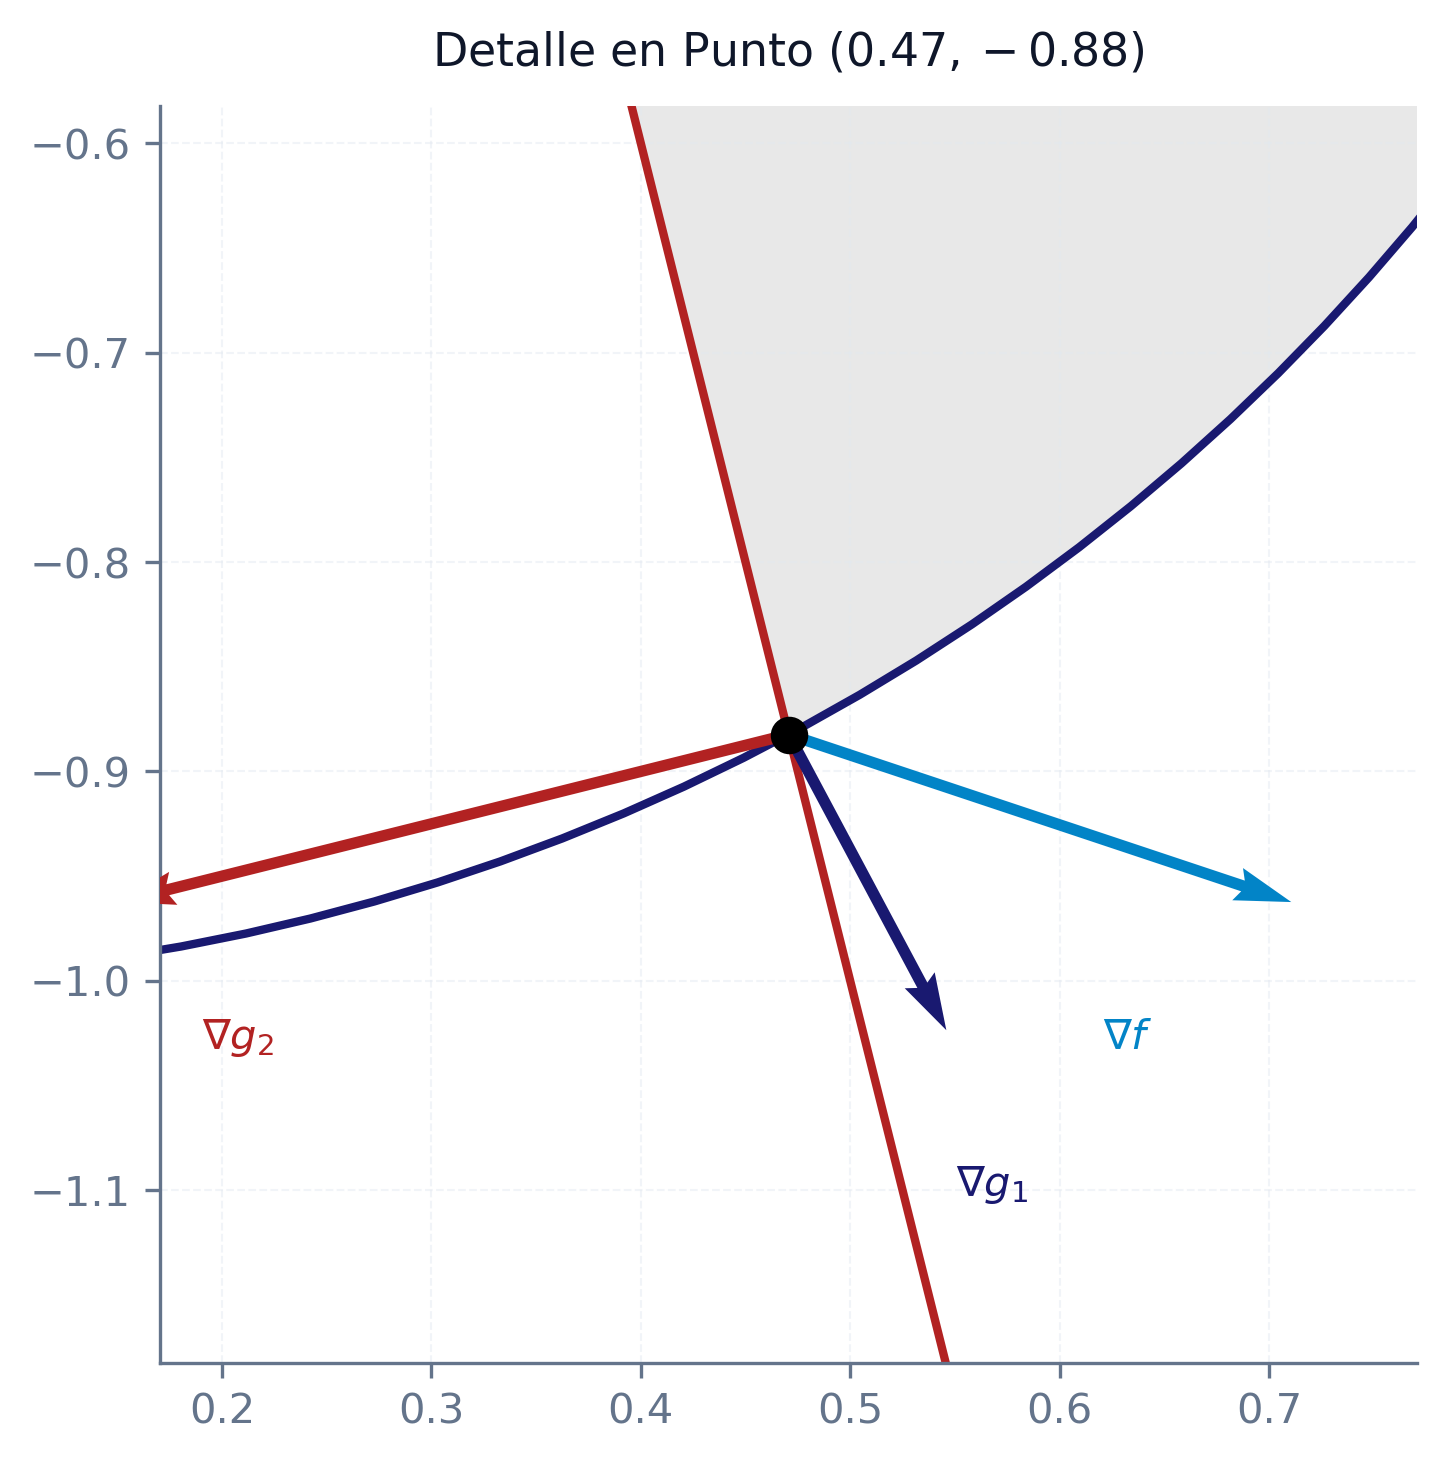
\includegraphics[width=0.6\linewidth,height=\textheight,keepaspectratio]{images/kkt_ejemplo_circ_lineal_zoom_d.png}

    }

    \caption{\label{fig-kkt-ejemplo-circ-lineal-zoom-d}KKT Restricción
    Circular y Lineal: Detalle en \((0.47, -0.88)\)}

    \end{figure}%
  \end{itemize}
\end{itemize}

\textbf{Conclusión y Caracterización de Candidatos}

Evaluamos las condiciones suficientes y comparamos los valores de la
función objetivo:

\begin{itemize}
\tightlist
\item
  \textbf{Mínimos}: El único candidato KKT a mínimo local es
  \textbf{\((0, 1)\)} con \(f(0, 1) = -1\).

  \begin{itemize}
  \tightlist
  \item
    La función objetivo \(f(x, y) = 3x - y\) es lineal (y por tanto,
    pseudo-convexa).
  \item
    La restricción \(g_1\) es estrictamente convexa y la restricción
    \(g_2\) es lineal (convexa), por lo que las restricciones activas en
    el punto son convexas (cuasi-convexas).
  \item
    Dado que \(u_1 = 7/8 > 0\) y \(u_2 = 3/4 > 0\), se satisfacen las
    condiciones suficientes de optimalidad global, lo que confirma que
    \textbf{\((0, 1)\) es el mínimo global}.
  \end{itemize}
\item
  \textbf{Máximos}: El único candidato KKT a máximo local es
  \textbf{\(\left(\frac{3}{\sqrt{10}}, -\frac{1}{\sqrt{10}}\right)\)}
  con
  \(f\left(\frac{3}{\sqrt{10}}, -\frac{1}{\sqrt{10}}\right) = \sqrt{10} \approx 3.16\).

  \begin{itemize}
  \tightlist
  \item
    La función objetivo \(f(x, y) = 3x - y\) es lineal (y por tanto,
    pseudo-cóncava).
  \item
    Las restricciones activas son cuasi-convexas.
  \item
    Dado que el multiplicador de la restricción activa es negativo
    (\(u_1 = -\sqrt{10}/2 < 0\)), se satisfacen las condiciones
    suficientes para máximos, confirmando que
    \textbf{\(\left(\frac{3}{\sqrt{10}}, -\frac{1}{\sqrt{10}}\right)\)
    es el máximo global}.
  \end{itemize}
\end{itemize}

En la Figura~\ref{fig-kkt-ejemplo-circ-lineal-conclusiones} se resume
gráficamente la caracterización final de los candidatos en este
problema.

\begin{figure}[H]

\centering{

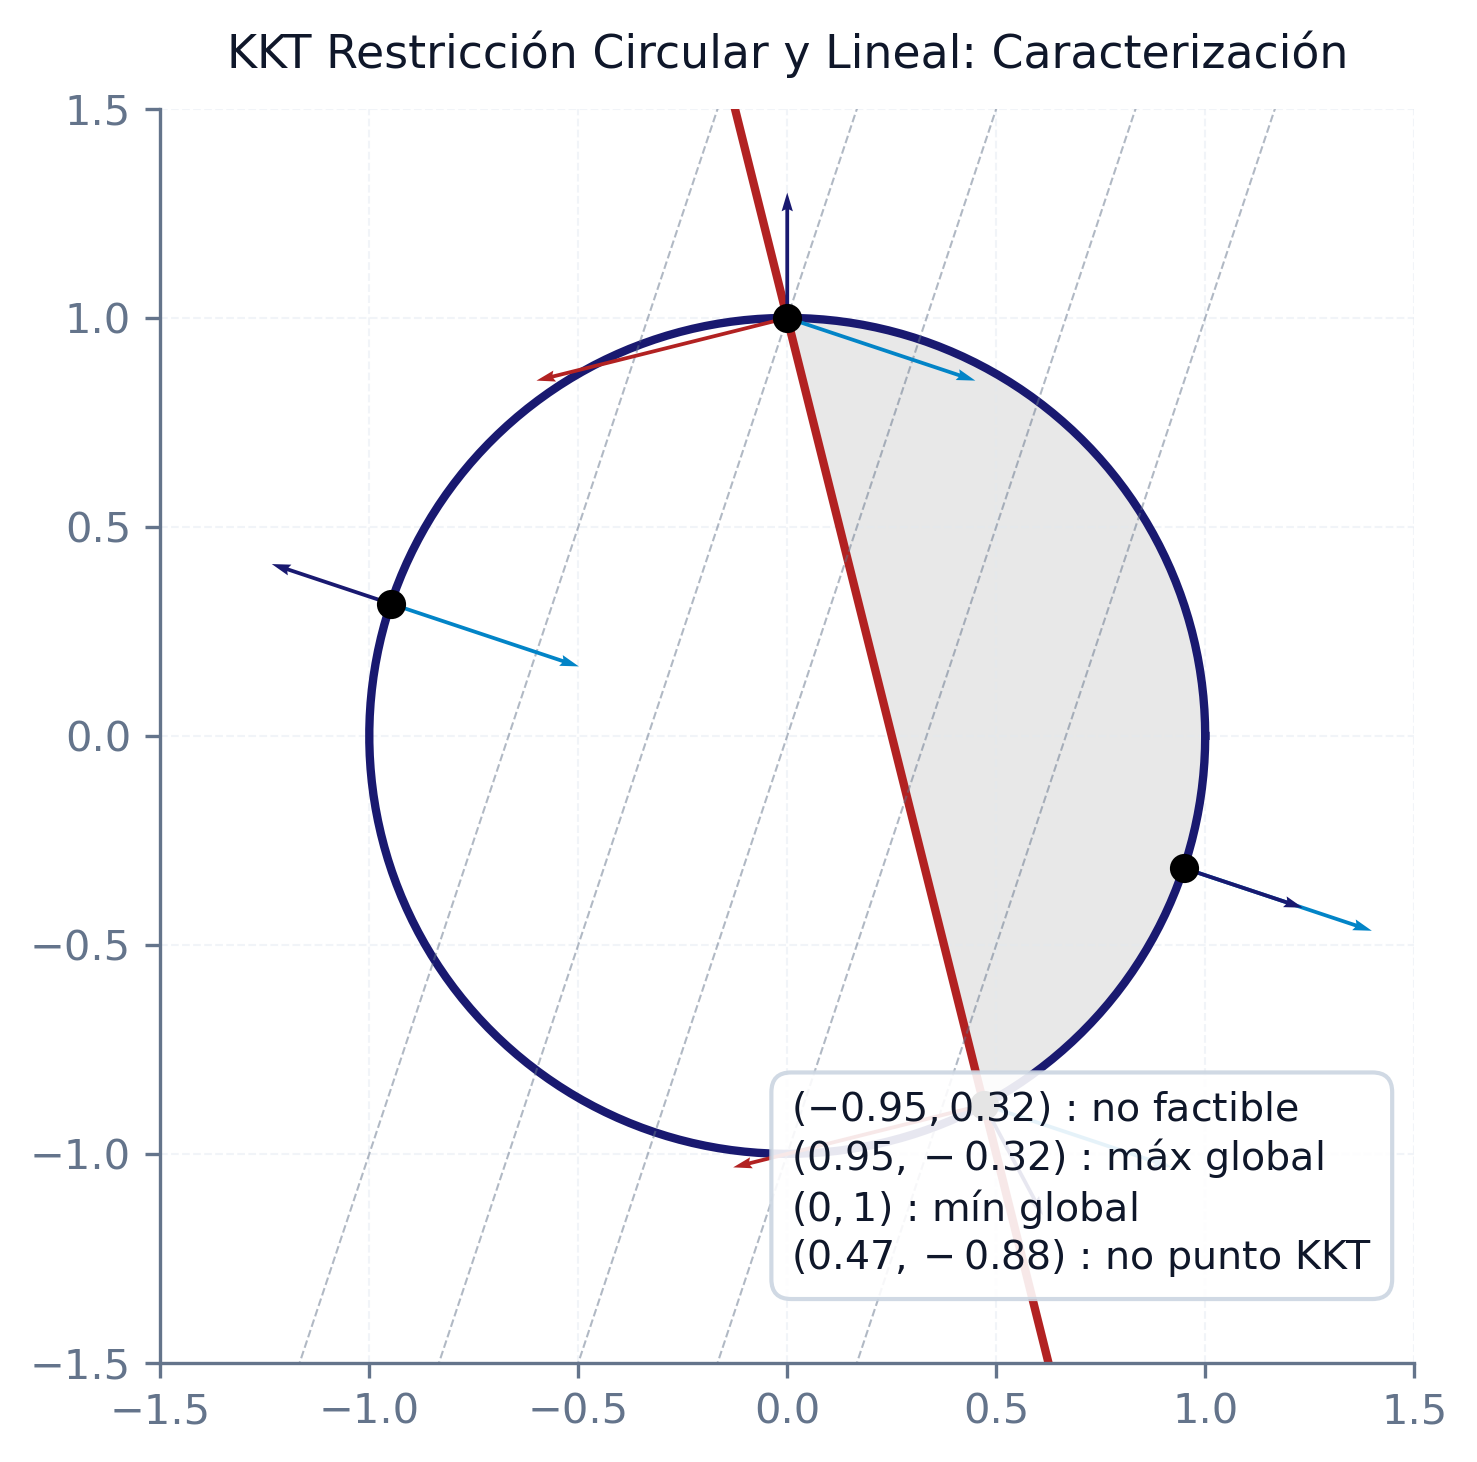
\includegraphics[width=0.75\linewidth,height=\textheight,keepaspectratio]{images/kkt_ejemplo_circ_lineal_conclusiones.png}

}

\caption{\label{fig-kkt-ejemplo-circ-lineal-conclusiones}KKT Restricción
Circular y Lineal: Caracterización}

\end{figure}%

\end{tcolorbox}

\section{Restricciones de igualdad y
desigualdad}\label{restricciones-de-igualdad-y-desigualdad}

Hasta este punto, el análisis de optimalidad se ha centrado en problemas
donde las restricciones limitan el espacio factible mediante
desigualdades (\(g_i(x) \le 0\)). Sin embargo, la formulación general de
los problemas de optimización matemática requiere frecuentemente la
inclusión de restricciones de igualdad de la forma \(h_j(x) = 0\), para
\(j=1,\dots,\ell\). Así, el problema general se define como:
\[ \min_{x} \{ f(x) \mid x \in \mathcal{X}, \ g_i(x) \le 0, \ i=1,\dots,m, \ h_j(x) = 0, \ j=1,\dots,\ell \} \]

Para extender las condiciones geométricas de optimalidad a este
escenario mixto, es necesario caracterizar la influencia de las
restricciones de igualdad sobre el conjunto de direcciones admisibles. A
diferencia de las desigualdades, que permiten movimientos hacia el
interior de la región factible, las restricciones de igualdad obligan a
que cualquier dirección admisible permanezca tangente a la
hipersuperficie definida por \(h_j(x) = 0\). Por ello, se define el cono
de direcciones tangentes al espacio de igualdad en un punto factible
\(\bar{x}\) como:
\[ \mathcal{H}_0(\bar{x}) = \{ d \in \mathbb{R}^n \mid \nabla h_j(\bar{x})^T d = 0, \ j = 1, \dots, \ell \} \]

Bajo esta definición, la condición necesaria de optimalidad geométrica
se formaliza mediante la exclusión de conos, estableciendo que en el
óptimo no pueden existir direcciones que desciendan la función objetivo,
que sean factibles para las desigualdades activas y que sean tangentes a
las igualdades simultáneamente.

\begin{tcolorbox}[enhanced jigsaw, toprule=.15mm, opacitybacktitle=0.6, coltitle=black, colbacktitle=quarto-callout-important-color!10!white, title=\textcolor{quarto-callout-important-color}{\faExclamation}\hspace{0.5em}{Teorema: Exclusión geométrica generalizada}, arc=.35mm, rightrule=.15mm, toptitle=1mm, breakable, bottomtitle=1mm, titlerule=0mm, colback=white, opacityback=0, leftrule=.75mm, colframe=quarto-callout-important-color-frame, left=2mm, bottomrule=.15mm]

Sea el problema:
\[ \min \{f(x) \mid x \in \mathcal{X}, \ g_i(x) \le 0, \ i=1,\dots,m, \ h_i(x) = 0, \ i=1,\dots,\ell\} \]
\(\bar{x}\) una solución factible del problema e \(\mathcal{I}\) el
conjunto de índices de las restricciones activas en \(\bar{x}\). Si se
verifican las siguientes propiedades: 1.
\(f, g_i, \ i \in \mathcal{I}\), son diferenciables en \(\bar{x}\), 2.
\(g_i, \ i \notin \mathcal{I}\), son continuas en \(\bar{x}\), 3.
\(h_i, \ i = 1, \dots, \ell\), son continuamente diferenciables en
\(\bar{x}\), 4. \(\nabla h_i, \ i = 1, \dots, \ell\), son linealmente
independientes en \(\bar{x}\), 5. \(\bar{x}\) es un mínimo local de
\(f\),

entonces,
\(\mathcal{D}_0(\bar{x}) \cap \mathcal{G}_0(\bar{x}) \cap \mathcal{H}_0(\bar{x}) = \emptyset\),
donde:
\[ \mathcal{G}_0(\bar{x}) = \{ d \in \mathbb{R}^n \mid \nabla g_i(\bar{x})^T d < 0, \ \forall i \in \mathcal{I} \} \quad \text{y} \quad \mathcal{H}_0(\bar{x}) = \{ d \in \mathbb{R}^n \mid \nabla h_i(\bar{x})^T d = 0, \ i = 1, \dots, \ell \} \]

\end{tcolorbox}

Esta exclusión geométrica se traduce al plano algebraico mediante la
aplicación de teoremas de alternativa, lo que da lugar a las condiciones
necesarias de Karush-Kuhn-Tucker (KKT) generales, siempre y cuando se
satisfaga la condición de regularidad (LICQ) en el punto óptimo.

\begin{tcolorbox}[enhanced jigsaw, toprule=.15mm, opacitybacktitle=0.6, coltitle=black, colbacktitle=quarto-callout-important-color!10!white, title=\textcolor{quarto-callout-important-color}{\faExclamation}\hspace{0.5em}{Teorema: Condiciones necesarias de Karush-Kuhn-Tucker (KKT)}, arc=.35mm, rightrule=.15mm, toptitle=1mm, breakable, bottomtitle=1mm, titlerule=0mm, colback=white, opacityback=0, leftrule=.75mm, colframe=quarto-callout-important-color-frame, left=2mm, bottomrule=.15mm]

Sea el problema
\(\min\{f(x) \mid x \in \mathcal{X}, \ g_i(x) \le 0, \ i=1,\dots,m, \ h_i(x)=0, \ i=1,\dots,\ell\}\),
\(\bar{x}\) una solución factible, e
\(\mathcal{I}=\{i \mid g_i(\bar{x}) = 0\}\) tal que:

\begin{enumerate}
\def\labelenumi{\arabic{enumi}.}
\tightlist
\item
  \(f, g_i, \ i \in \mathcal{I}\) son diferenciables en \(\bar{x}\),
\item
  \(g_i, \ i \notin \mathcal{I}\) son continuas en \(\bar{x}\),
\item
  \(h_i, \ i=1,\dots,\ell\) son continuamente diferenciables en
  \(\bar{x}\), y
\item
  \(\nabla g_i(\bar{x}), \ i \in \mathcal{I}\) y
  \(\nabla h_i(\bar{x}), \ i=1,\dots,\ell\) son linealmente
  independientes en \(\bar{x}\).
\end{enumerate}

Entonces, si \(\bar{x}\) es un mínimo local de \(f\), existen escalares
\(\{u_i, \ i \in \mathcal{I}, \ v_j, \ j=1,\dots,\ell\}\), con
\(u_i \ge 0\), \(\forall i \in \mathcal{I}\) tales que:
\[ \nabla f(\bar{x}) + \sum_{i \in \mathcal{I}} u_i \nabla g_i(\bar{x}) + \sum_{j=1}^\ell v_j \nabla h_j(\bar{x}) = 0 \]

Si además se verifica que las funciones
\(\{g_i, \ i \notin \mathcal{I}\}\) son diferenciables en \(\bar{x}\),
las condiciones anteriores se pueden escribir de la forma: \[
\begin{aligned}
\nabla f(\bar{x}) + \sum_{i=1}^m u_i \nabla g_i(\bar{x}) + \sum_{j=1}^\ell v_j \nabla h_j(\bar{x}) &= 0 \\
u_i g_i(\bar{x}) &= 0, \quad \forall i=1,\dots,m \\
u_i &\ge 0, \quad \forall i=1,\dots,m
\end{aligned}
\]

\end{tcolorbox}

Es fundamental resaltar la diferencia matemática y física entre ambos
tipos de multiplicadores: mientras que los multiplicadores \(u_i\)
correspondientes a las desigualdades deben ser obligatoriamente no
negativos (\(u_i \ge 0\)) para asegurar que las direcciones de descenso
no se solapen con las factibles, los multiplicadores \(v_j\) asociados a
las restricciones de igualdad no poseen restricción de signo
(\(v_j \in \mathbb{R}\)), puesto que el movimiento admisible sobre la
hipersuperficie está restringido en ambas direcciones (tanto a favor
como en contra de \(\nabla h_j(\bar{x})\)).

Para ilustrar el funcionamiento de estas condiciones en presencia de
restricciones mixtas, resolveremos detalladamente dos problemas de
optimización sobre la misma región factible acotada por un círculo, la
restricción de no negatividad de las variables (primer cuadrante) y una
restricción lineal de igualdad, considerando dos configuraciones
lineales distintas.

\begin{tcolorbox}[enhanced jigsaw, toprule=.15mm, opacitybacktitle=0.6, coltitle=black, colbacktitle=quarto-callout-tip-color!10!white, title=\textcolor{quarto-callout-tip-color}{\faLightbulb}\hspace{0.5em}{Ejemplo: Restricciones mixtas con frontera \(x_1 + x_2 - 3 = 0\)}, arc=.35mm, rightrule=.15mm, toptitle=1mm, breakable, bottomtitle=1mm, titlerule=0mm, colback=white, opacityback=0, leftrule=.75mm, colframe=quarto-callout-tip-color-frame, left=2mm, bottomrule=.15mm]

Consideremos el problema de encontrar los mínimos locales de dos
funciones objetivo distintas sobre la región definida en
\(\mathbb{R}^2\) por: \[
\begin{aligned}
\min \quad & f(x_1, x_2) \\
\text{s.a.} \quad & g_1(x_1, x_2) = x_1^2 + x_2^2 - 5 \le 0 \\
& g_2(x_1, x_2) = -x_1 \le 0 \\
& g_3(x_1, x_2) = -x_2 \le 0 \\
& h_1(x_1, x_2) = x_1 + x_2 - 3 = 0
\end{aligned}
\] Las funciones objetivo a evaluar son: 1.
\(f_1(x_1, x_2) = x_1^2 + x_2^2\) (que representa la distancia al origen
al cuadrado). 2. \(f_2(x_1, x_2) = (x_1 - 3)^2 + (x_2 - 2)^2\) (que
representa la distancia al cuadrado al punto \((3,2)\)).

Geométricamente (ver Figura~\ref{fig-kkt-mixtas-ejemplo1}), la región
factible \(\mathcal{S}\) se reduce al segmento de la recta
\(x_1 + x_2 = 3\) que yace dentro de la circunferencia de radio
\(\sqrt{5}\) en el primer cuadrante. Para determinar dicho segmento,
sustituimos \(x_2 = 3 - x_1\) en la circunferencia:
\[ x_1^2 + (3-x_1)^2 \le 5 \implies 2x_1^2 - 6x_1 + 4 \le 0 \implies (x_1 - 1)(x_1 - 2) \le 0 \implies x_1 \in [1, 2] \]
Por tanto, el dominio factible es el segmento de extremos \((1,2)\) y
\((2,1)\). La función Lagrangiana común es:
\[ L(x_1, x_2, u, v) = f(x_1, x_2) + u_1(x_1^2 + x_2^2 - 5) + u_2(-x_1) + u_3(-x_2) + v_1(x_1 + x_2 - 3) \]

\textbf{Resolución para \(f_1(x_1, x_2) = x_1^2 + x_2^2\):}

\begin{itemize}
\tightlist
\item
  \textbf{Caso A (Interior del segmento factible, \(x_1 \in (1, 2)\))}:
  Las restricciones de desigualdad son inactivas
  (\(u_1 = u_2 = u_3 = 0\)). El sistema de estacionariedad exige:
  \[ \begin{aligned} 2x_1 + v_1 &= 0 \\ 2x_2 + v_1 &= 0 \end{aligned} \implies x_1 = x_2 \]
  Dado que la igualdad \(h_1\) exige \(x_1 + x_2 = 3\), obtenemos el
  punto \textbf{\((1.5, 1.5)\)} con \(v_1 = -3\). Dado que este punto es
  factible, constituye un candidato KKT a mínimo local (siendo el mínimo
  global con \(f_1 = 4.5\)).
\item
  \textbf{Caso B (Extremos del segmento factible)}:

  \begin{itemize}
  \tightlist
  \item
    \emph{Punto \((1, 2)\)}: Activa \(g_1\) y \(h_1\)
    (\(u_2 = u_3 = 0\)). La estacionariedad plantea:
    \[ \begin{aligned} 2 + 2u_1 + v_1 &= 0 \\ 4 + 4u_1 + v_1 &= 0 \end{aligned} \implies 2 + 2u_1 = 0 \implies u_1 = -1 < 0 \]
    Dado que el multiplicador \(u_1\) es negativo, este punto no es
    candidato a mínimo.
  \item
    \emph{Punto \((2, 1)\)}: Por simetría directa, se obtiene igualmente
    \(u_1 = -1 < 0\), descartándolo como candidato a mínimo.
  \end{itemize}
\end{itemize}

\textbf{Resolución para \(f_2(x_1, x_2) = (x_1 - 3)^2 + (x_2 - 2)^2\):}

\begin{itemize}
\tightlist
\item
  \textbf{Caso A (Interior del segmento factible, \(x_1 \in (1, 2)\))}:
  Con \(u_1 = u_2 = u_3 = 0\), la estacionariedad es:
  \[ \begin{aligned} 2(x_1 - 3) + v_1 &= 0 \\ 2(x_2 - 2) + v_1 &= 0 \end{aligned} \implies x_1 - 3 = x_2 - 2 \implies x_1 = x_2 + 1 \]
  Sustituyendo en la igualdad:
  \((x_2 + 1) + x_2 = 3 \implies 2x_2 = 2 \implies x_2 = 1, x_1 = 2\).
  Dado que esta solución corresponde al extremo del segmento, no existen
  puntos estacionarios en el interior del mismo.
\item
  \textbf{Caso B (Extremos del segmento factible)}:

  \begin{itemize}
  \tightlist
  \item
    \emph{Punto \((1, 2)\)}: Con \(u_2=u_3=0\), la estacionariedad
    plantea:
    \[ \begin{aligned} 2(1-3) + 2u_1 + v_1 &= 0 \implies -4 + 2u_1 + v_1 = 0 \\ 2(2-2) + 4u_1 + v_1 &= 0 \implies 4u_1 + v_1 = 0 \end{aligned} \]
    Restando ambas ecuaciones: \(-4 - 2u_1 = 0 \implies u_1 = -2 < 0\).
    Se descarta por el signo del multiplicador.
  \item
    \emph{Punto \((2, 1)\)}: Con \(u_2=u_3=0\), la estacionariedad
    plantea:
    \[ \begin{aligned} 2(2-3) + 4u_1 + v_1 &= 0 \implies -2 + 4u_1 + v_1 = 0 \\ 2(1-2) + 2u_1 + v_1 &= 0 \implies -2 + 2u_1 + v_1 = 0 \end{aligned} \]
    Restando ambas ecuaciones: \(2u_1 = 0 \implies u_1 = 0\).
    Sustituyendo, obtenemos \(v_1 = 2\). Como \(u_1 = 0 \ge 0\), el
    punto \textbf{\((2, 1)\)} satisface las condiciones KKT y es el
    candidato a mínimo local (mínimo global con \(f_2 = 2.0\)).
  \end{itemize}
\end{itemize}

\begin{figure}[H]

\centering{

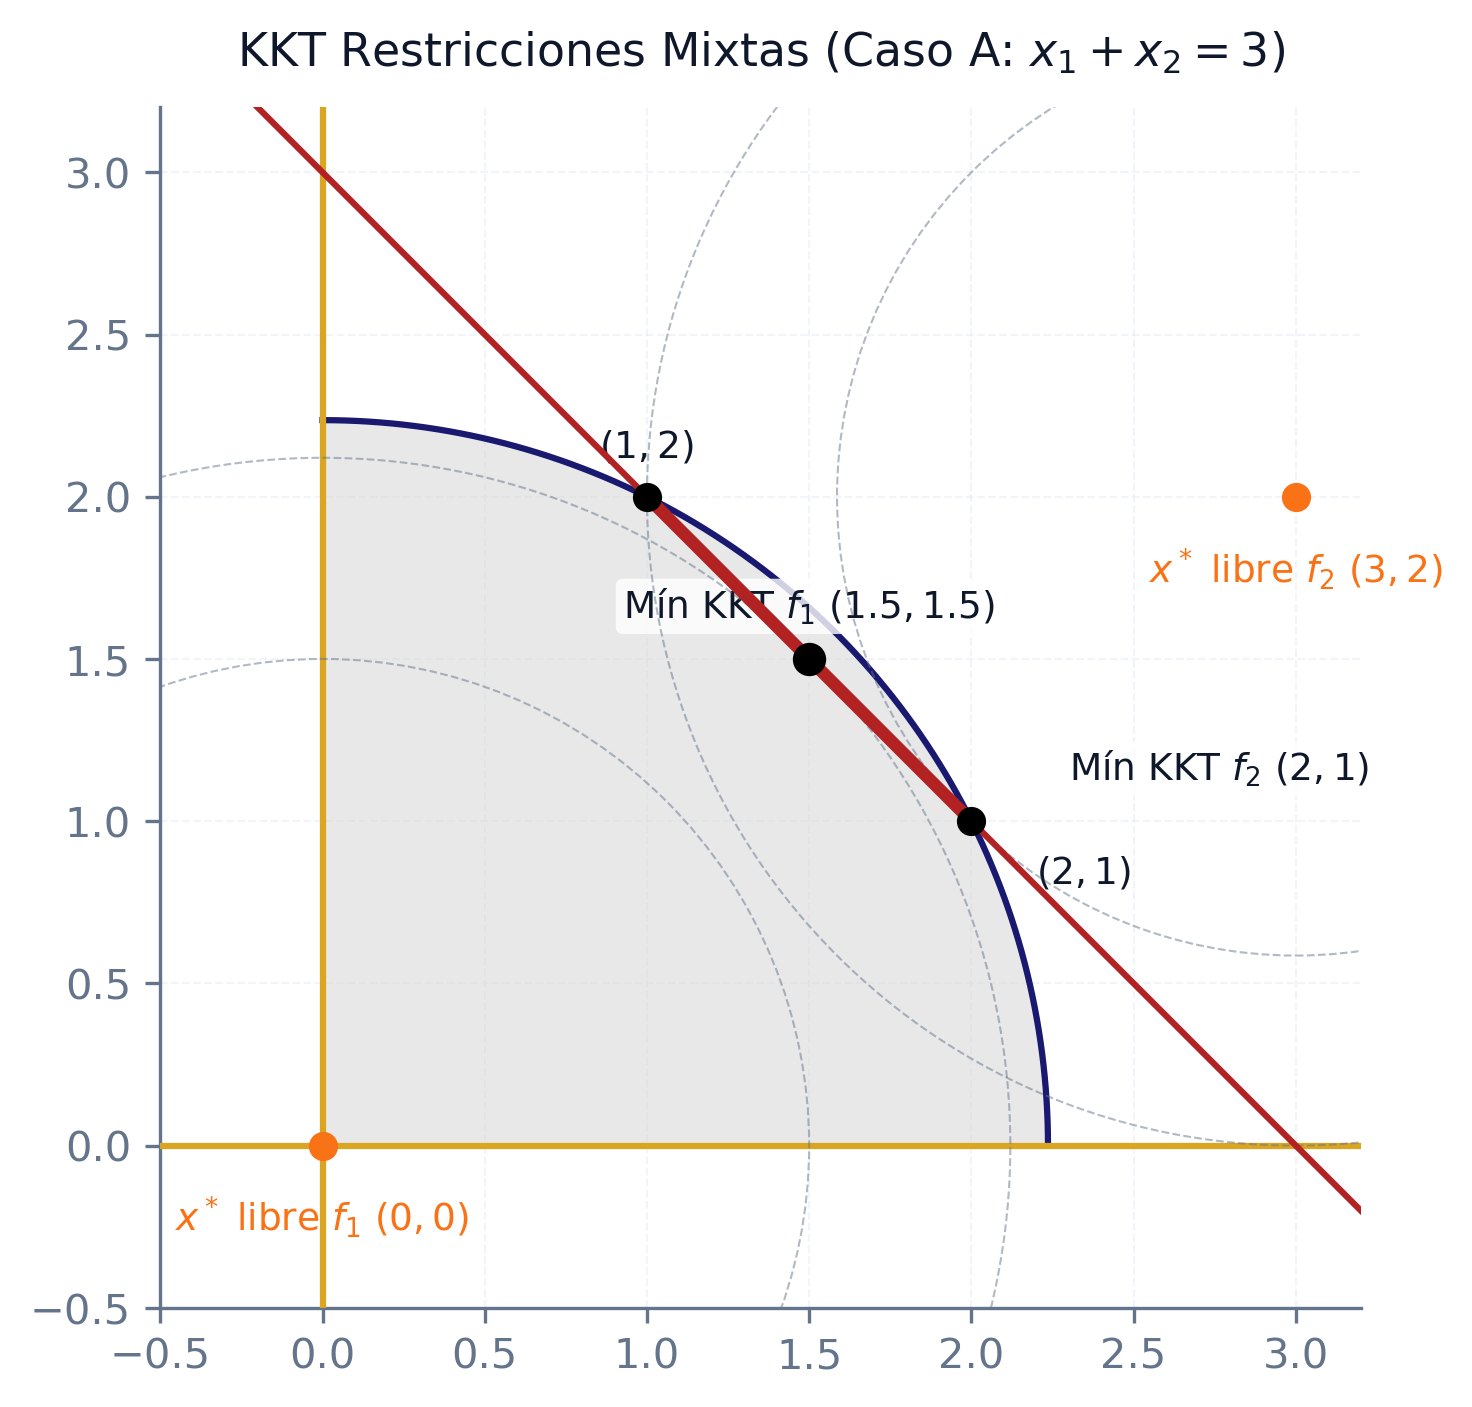
\includegraphics[width=0.6\linewidth,height=\textheight,keepaspectratio]{images/kkt_mixtas_ejemplo1.png}

}

\caption{\label{fig-kkt-mixtas-ejemplo1}Análisis KKT mixto para
\(x_1 + x_2 = 3\)}

\end{figure}%

\end{tcolorbox}

\begin{tcolorbox}[enhanced jigsaw, toprule=.15mm, opacitybacktitle=0.6, coltitle=black, colbacktitle=quarto-callout-tip-color!10!white, title=\textcolor{quarto-callout-tip-color}{\faLightbulb}\hspace{0.5em}{Ejemplo: Restricciones mixtas con frontera \(x_1 + 2x_2 - 4 = 0\)}, arc=.35mm, rightrule=.15mm, toptitle=1mm, breakable, bottomtitle=1mm, titlerule=0mm, colback=white, opacityback=0, leftrule=.75mm, colframe=quarto-callout-tip-color-frame, left=2mm, bottomrule=.15mm]

Consideremos ahora el mismo problema de optimización pero modificando la
restricción de igualdad a: \[ h_1(x_1, x_2) = x_1 + 2x_2 - 4 = 0 \] Las
funciones objetivo siguen siendo \(f_1(x_1, x_2) = x_1^2 + x_2^2\) y
\(f_2(x_1, x_2) = (x_1 - 3)^2 + (x_2 - 2)^2\).

Geométricamente (ver Figura~\ref{fig-kkt-mixtas-ejemplo2}), la región
factible \(\mathcal{S}\) se reduce al segmento de la recta
\(x_1 + 2x_2 = 4\) dentro del primer cuadrante y del círculo de radio
\(\sqrt{5}\). Determinemos el rango factible de \(x_2\) sustituyendo
\(x_1 = 4 - 2x_2\) en la circunferencia:
\[ (4 - 2x_2)^2 + x_2^2 \le 5 \implies 5x_2^2 - 16x_2 + 11 \le 0 \implies (x_2 - 1)(5x_2 - 11) \le 0 \implies x_2 \in [1, 2.2] \]
No obstante, para asegurar la factibilidad en el primer cuadrante,
también debe cumplirse
\(x_1 \ge 0 \implies 4 - 2x_2 \ge 0 \implies x_2 \le 2\). Así, la región
factible real es el segmento de extremos \((2,1)\) (para \(x_2 = 1\)) y
\((0,2)\) (para \(x_2 = 2\)).

\textbf{Resolución para \(f_1(x_1, x_2) = x_1^2 + x_2^2\):}

\begin{itemize}
\tightlist
\item
  \textbf{Caso A (Interior del segmento factible, \(x_2 \in (1, 2)\))}:
  Las restricciones de desigualdad son inactivas
  (\(u_1 = u_2 = u_3 = 0\)). La estacionariedad con \(h_1\) exige:
  \[ \begin{aligned} 2x_1 + v_1 &= 0 \\ 2x_2 + 2v_1 &= 0 \end{aligned} \implies x_2 = 2x_1 \]
  Sustituyendo en la restricción de igualdad:
  \(x_1 + 2(2x_1) = 4 \implies 5x_1 = 4 \implies x_1 = 0.8\), lo que da
  \(x_2 = 1.6\). El punto obtenido es \textbf{\((0.8, 1.6)\)} con
  \(v_1 = -1.6\). Dado que es factible, constituye un candidato KKT a
  mínimo local (y mínimo global con \(f_1 = 3.2\)).
\item
  \textbf{Caso B (Extremos del segmento factible)}:

  \begin{itemize}
  \tightlist
  \item
    \emph{Punto \((2, 1)\)}: Activa \(g_1\) y \(h_1\)
    (\(u_2 = u_3 = 0\)). La estacionariedad plantea:
    \[ \begin{aligned} 4 + 4u_1 + v_1 &= 0 \\ 2 + 2u_1 + 2v_1 &= 0 \implies 1 + u_1 + v_1 = 0 \implies v_1 = -1 - u_1 \end{aligned} \]
    Sustituyendo en la primera:
    \(4 + 4u_1 - 1 - u_1 = 0 \implies u_1 = -1 < 0\). Se descarta.
  \item
    \emph{Punto \((0, 2)\)}: Activa el eje \(g_2(x) = -x_1 \le 0\) y la
    recta \(h_1 = 0\) (\(u_1 = u_3 = 0\)). La estacionariedad plantea:
    \[ \begin{aligned} 0 - u_2 + v_1 &= 0 \implies u_2 = v_1 \\ 4 + 2v_1 &= 0 \implies v_1 = -2 \implies u_2 = -2 < 0 \end{aligned} \]
    Se descarta por tener un multiplicador de desigualdad negativo.
  \end{itemize}
\end{itemize}

\textbf{Resolución para \(f_2(x_1, x_2) = (x_1 - 3)^2 + (x_2 - 2)^2\):}

\begin{itemize}
\tightlist
\item
  \textbf{Caso A (Interior del segmento factible, \(x_2 \in (1, 2)\))}:
  Con \(u_1 = u_2 = u_3 = 0\), la estacionariedad plantea:
  \[ \begin{aligned} 2(x_1 - 3) + v_1 &= 0 \\ 2(x_2 - 2) + 2v_1 &= 0 \end{aligned} \implies x_2 - 2 = 2(x_1 - 3) \implies x_2 = 2x_1 - 4 \]
  Sustituyendo en la igualdad:
  \(x_1 + 2(2x_1 - 4) = 4 \implies 5x_1 = 12 \implies x_1 = 2.4, x_2 = 0.8\).
  Dado que \(x_2 = 0.8 < 1\), esta solución cae fuera del segmento
  factible y se descarta.
\item
  \textbf{Caso B (Extremos del segmento factible)}:

  \begin{itemize}
  \tightlist
  \item
    \emph{Punto \((2, 1)\)}: Activa \(g_1\) y \(h_1\)
    (\(u_2 = u_3 = 0\)). La estacionariedad plantea:
    \[ \begin{aligned} 2(2-3) + 4u_1 + v_1 &= 0 \implies -2 + 4u_1 + v_1 = 0 \\ 2(1-2) + 2u_1 + 2v_1 &= 0 \implies -2 + 2u_1 + 2v_1 = 0 \implies -1 + u_1 + v_1 = 0 \end{aligned} \]
    De la segunda obtenemos \(v_1 = 1 - u_1\). Sustituyendo en la
    primera:
    \(-2 + 4u_1 + 1 - u_1 = 0 \implies 3u_1 = 1 \implies u_1 = 1/3 \ge 0\).
    Esto nos da \(v_1 = 2/3\). Al obtener multiplicadores factibles, el
    punto \textbf{\((2, 1)\)} es un candidato KKT a mínimo local (mínimo
    global con \(f_2 = 2.0\)).
  \item
    \emph{Punto \((0, 2)\)}: Activa \(g_2\) y \(h_1\)
    (\(u_1 = u_3 = 0\)). La estacionariedad plantea:
    \[ \begin{aligned} 2(0-3) - u_2 + v_1 &= 0 \implies -6 - u_2 + v_1 = 0 \\ 2(2-2) + 2v_1 &= 0 \implies 2v_1 = 0 \implies v_1 = 0 \end{aligned} \]
    Lo que da \(u_2 = -6 < 0\). Se descarta.
  \end{itemize}
\end{itemize}

\begin{figure}[H]

\centering{

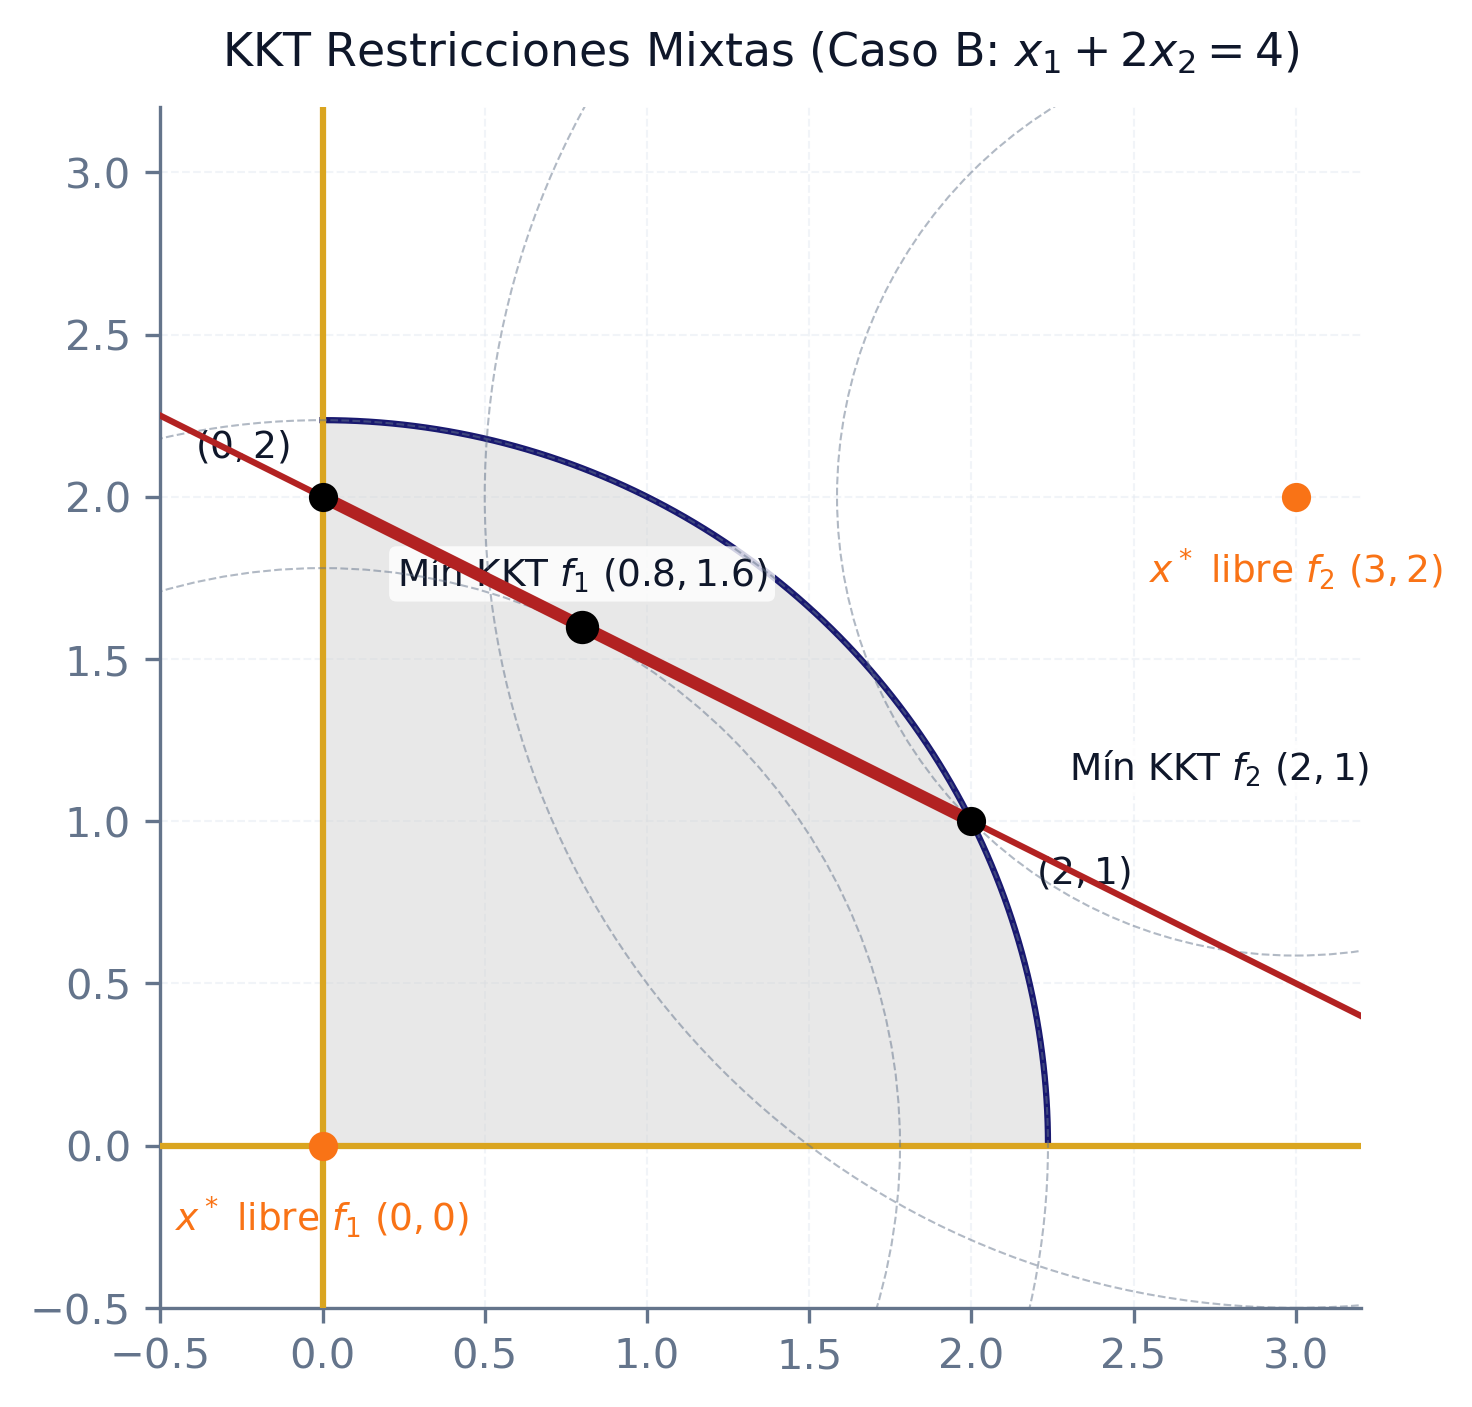
\includegraphics[width=0.6\linewidth,height=\textheight,keepaspectratio]{images/kkt_mixtas_ejemplo2.png}

}

\caption{\label{fig-kkt-mixtas-ejemplo2}Análisis KKT mixto para
\(x_1 + 2x_2 = 4\)}

\end{figure}%

\end{tcolorbox}

\chapter{Programación lineal y
cuadrática}\label{programaciuxf3n-lineal-y-cuadruxe1tica}

Las condiciones de Karush-Kuhn-Tucker (KKT) adquieren una relevancia
excepcional al aplicarse sobre problemas con estructuras matemáticas
específicas, como la \textbf{Programación Lineal (LP)} y la
\textbf{Programación Cuadrática (QP)}. En ambos casos, las restricciones
son afines, lo que garantiza que las cualificaciones de restricciones
(como LICQ) se verifiquen de forma natural en cualquier punto factible.
Además, cuando la función objetivo es convexa, las condiciones
necesarias de KKT se convierten también en suficientes, proporcionando
un marco algebraico cerrado para hallar y certificar el óptimo global.

En este capítulo, analizaremos la relación profunda entre las
condiciones KKT y la dualidad lineal, explicaremos la interpretación
económica de las variables duales como precios sombra, clasificaremos la
correspondencia de los distintos tipos de óptimos lineales mediante
ilustraciones geométricas paso a paso, describiremos la estructura
matricial de la programación cuadrática y detallaremos el método del
Símplex de Wolfe para resolver problemas cuadráticos convexos.

\begin{tcolorbox}[enhanced jigsaw, toprule=.15mm, opacitybacktitle=0.6, coltitle=black, colbacktitle=quarto-callout-important-color!10!white, title=\textcolor{quarto-callout-important-color}{\faExclamation}\hspace{0.5em}{Objetivos de aprendizaje}, arc=.35mm, rightrule=.15mm, toptitle=1mm, breakable, bottomtitle=1mm, titlerule=0mm, colback=white, opacityback=0, leftrule=.75mm, colframe=quarto-callout-important-color-frame, left=2mm, bottomrule=.15mm]

Al finalizar este capítulo, serás capaz de:

\begin{enumerate}
\def\labelenumi{\arabic{enumi}.}
\tightlist
\item
  \textbf{Deducir y justificar} la equivalencia entre los
  multiplicadores KKT de un problema de programación lineal y las
  variables óptimas de su problema dual asociado.
\item
  \textbf{Demostrar formalmente} el teorema de dualidad débil en
  programación lineal y deducir sus consecuencias sobre el salto dual y
  la no acotación.
\item
  \textbf{Interpretar económicamente} las variables duales como precios
  sombra (\emph{shadow prices}) de los términos independientes.
\item
  \textbf{Clasificar los tipos de óptimos} en programación lineal
  atendiendo a la unicidad, degeneración y acotación tanto del problema
  primal como del dual.
\item
  \textbf{Formular el sistema KKT} para problemas de programación
  cuadrática (QP) en forma matricial.
\item
  \textbf{Aplicar el algoritmo del Símplex de Wolfe} (regla de entrada
  restringida) para resolver de forma exacta problemas cuadráticos
  convexos.
\end{enumerate}

\end{tcolorbox}

\section{Programación lineal (LP)}\label{programaciuxf3n-lineal-lp}

La \textbf{Programación Lineal (LP)} representa la piedra angular de la
optimización matemática moderna y de la investigación operativa (Hillier
y Lieberman 2010; Bazaraa, Jarvis, y Sherali 2011; Luenberger y Ye
2015). Consiste en la optimización (minimización o maximización) de un
criterio de rendimiento lineal expresado por un vector de costes
\(c \in \mathbb{R}^n\), sobre un conjunto de soluciones factibles
delimitado exclusivamente por hiperplanos y semiespacios afines dados
por restricciones de igualdad o desigualdad lineal.

Desde una perspectiva geométrica, el conjunto factible de un problema de
programación lineal constituye un \textbf{poliedro convexo} (un politopo
si está acotado). Como consecuencia directa de la convexidad del
conjunto y de la linealidad de la función objetivo, la programación
lineal posee dos propiedades geométricas fundamentales:

\begin{enumerate}
\def\labelenumi{\arabic{enumi}.}
\tightlist
\item
  \textbf{Ausencia de óptimos locales strictly disjuntos}: Todo mínimo
  local es automáticamente un mínimo global.
\item
  \textbf{Teorema Fundamental de la Programación Lineal}: Si el problema
  admite solución óptima finita y la región factible posee al menos un
  punto extremo (vértice), existe al menos un \textbf{vértice extremo}
  del poliedro donde se alcanza dicho óptimo global.
\end{enumerate}

Como se ilustra en la Figura~\ref{fig-region-factible-lp}, la geometría
de la programación lineal se caracteriza por una región factible
poliédrica cuyos bordes son las restricciones afines activas, sobre la
cual la función objetivo desplaza sus curvas de nivel hiperplánicas en
la dirección de máximo descenso dictada por el vector gradiente del
coste \(c\).

\begin{figure}

\centering{

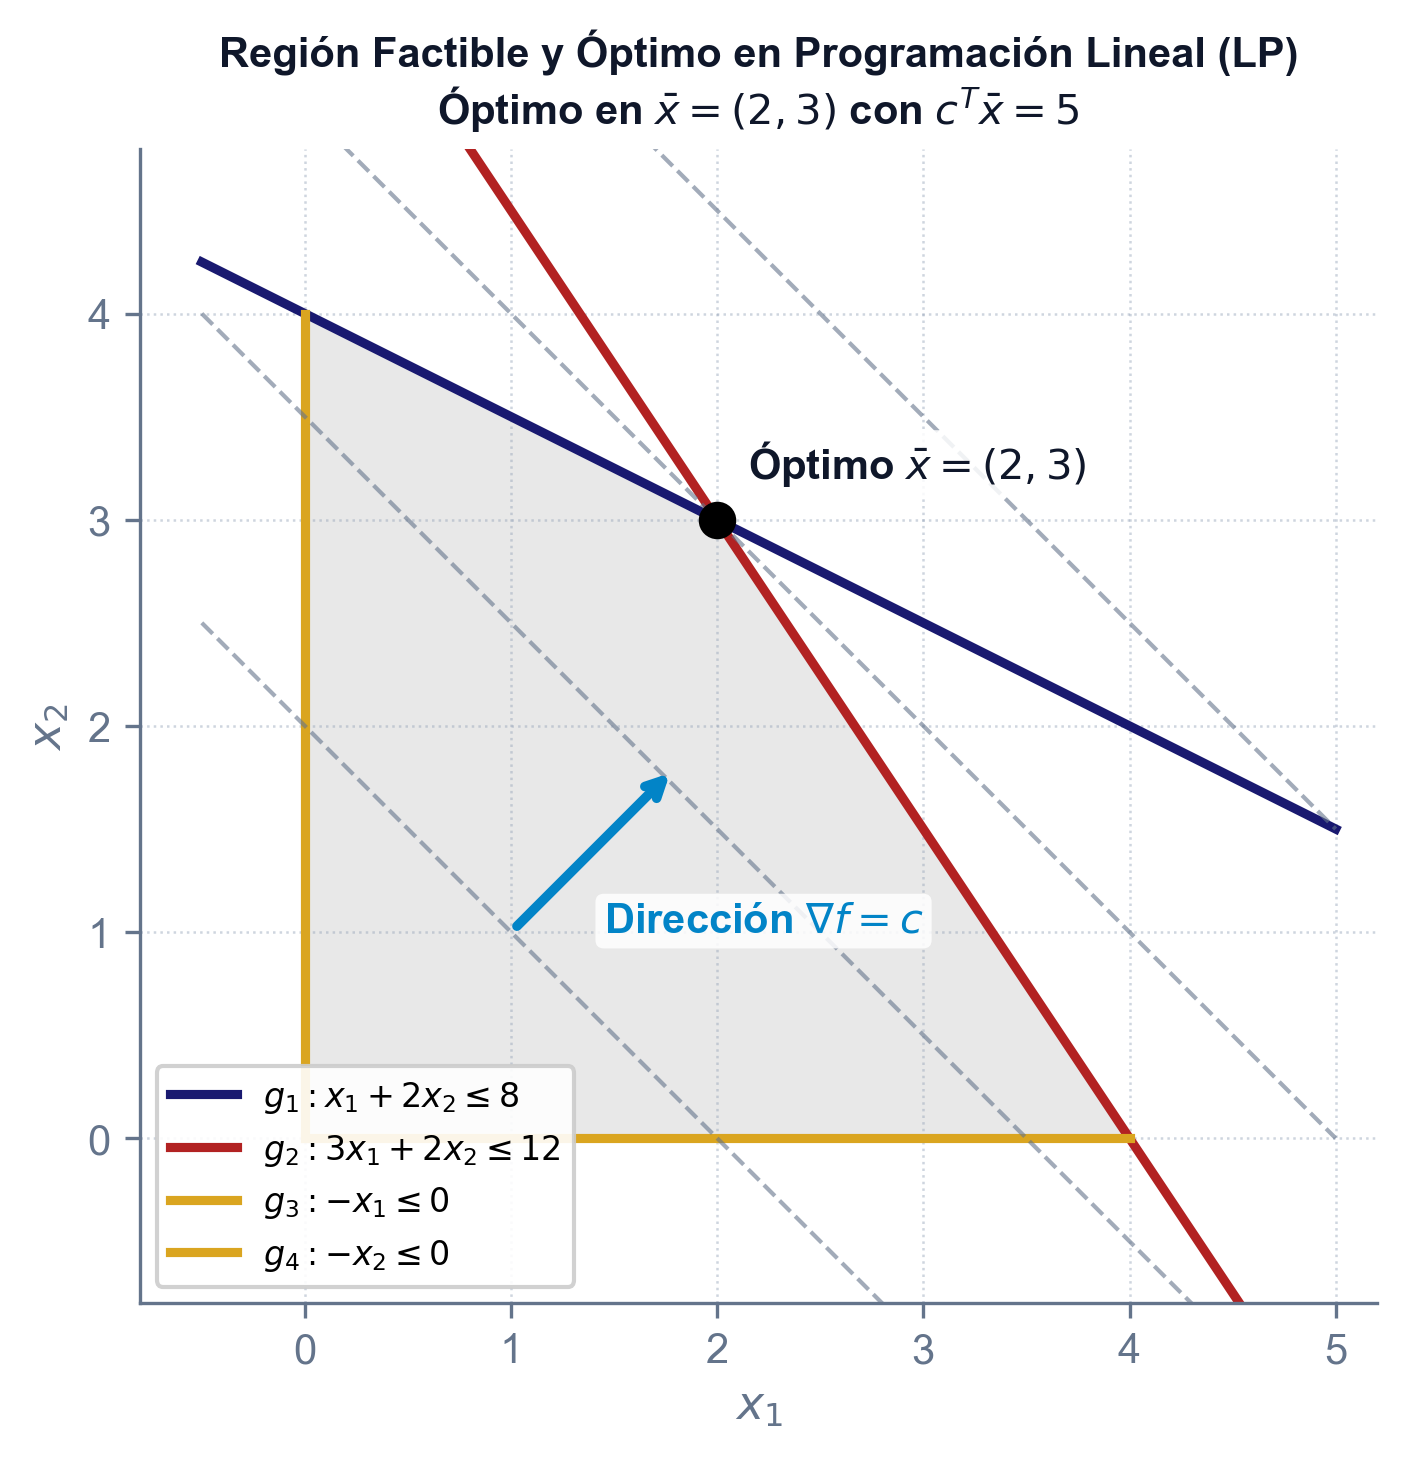
\includegraphics[width=0.7\linewidth,height=\textheight,keepaspectratio]{images/region_factible_lp.png}

}

\caption{\label{fig-region-factible-lp}Región factible y dirección de
optimización en un problema de programación lineal}

\end{figure}%

\subsection{Dualidad en programación
lineal}\label{dualidad-en-programaciuxf3n-lineal}

El concepto de dualidad constituye uno de los pilares más profundos e
insustituibles de la optimización lineal. A todo problema de
programación lineal, denominado \textbf{problema primal}, se le asocia
de forma simétrica e involutiva otro problema lineal estrechamente
vinculado denominado \textbf{problema dual}. La teoría de la dualidad
establece que ambos problemas observan la misma situación de
optimización desde dos perspectivas complementarias: mientras que el
problema primal busca asignar niveles de actividad para minimizar un
coste total (o maximizar un beneficio) sujeto a restricciones afines
generales, el problema dual busca determinar la valoración económica
óptima de dichos términos independientes.

Analíticamente, el problema primal original (P) se formula en su forma
canónica de minimización como:

\[
\begin{aligned}
\min_{x \in \mathbb{R}^n} \quad & c^T x \\
\text{sujeto a} \quad & A x \ge b \\
& x \ge 0
\end{aligned}
\]

donde \(x \in \mathbb{R}^n\) representa el vector de variables primales,
\(c \in \mathbb{R}^n\) el vector de costes,
\(A \in \mathbb{R}^{m \times n}\) la matriz de coeficientes de las
restricciones y \(b \in \mathbb{R}^m\) la términos independientes.

Asociando un vector de multiplicadores o variables duales
\(w \in \mathbb{R}^m\) (\(w \ge 0\)) a las \(m\) restricciones afines
generales \(A x \ge b\), se construye de forma natural el
\textbf{problema dual (D)} equivalente en forma canónica de
maximización:

\[
\begin{aligned}
\max_{w \in \mathbb{R}^m} \quad & b^T w \\
\text{sujeto a} \quad & A^T w \le c \\
& w \ge 0
\end{aligned}
\]

Esta relación dual posee la propiedad simétrica fundamental de
involución: el problema dual del problema dual es exactamente el
problema primal original.

La relación entre los valores objetivos de ambos problemas queda
establecida fundamentalmente por el teorema de dualidad débil:

\begin{tcolorbox}[enhanced jigsaw, toprule=.15mm, opacitybacktitle=0.6, coltitle=black, colbacktitle=quarto-callout-important-color!10!white, title=\textcolor{quarto-callout-important-color}{\faExclamation}\hspace{0.5em}{Teorema: Teorema de dualidad débil en LP}, arc=.35mm, rightrule=.15mm, toptitle=1mm, breakable, bottomtitle=1mm, titlerule=0mm, colback=white, opacityback=0, leftrule=.75mm, colframe=quarto-callout-important-color-frame, left=2mm, bottomrule=.15mm]

Para cualquier solución factible \(x\) del problema primal (P) y
cualquier solución factible \(w\) del problema dual (D), el valor de la
función objetivo dual es una cota inferior del valor de la función
objetivo primal: \[ b^T w \le c^T x \]

\emph{Demostración}:

\begin{enumerate}
\def\labelenumi{\arabic{enumi}.}
\tightlist
\item
  \textbf{Factibilidad primal}: Sea \(x\) una solución factible en (P),
  lo que implica que \(A x \ge b\). Multiplicando por la izquierda por
  el vector dual no negativo \(w^T \ge 0\) (\(w\) factible dual), se
  preserva el sentido de la desigualdad: \[ w^T b \le w^T A x \]
\item
  \textbf{Factibilidad dual}: Sea \(w\) una solución factible en (D), lo
  que implica que \(A^T w \le c \iff w^T A \le c^T\). Multiplicando por
  la derecha por el vector primal no negativo \(x \ge 0\), se preserva
  el sentido de la desigualdad: \[ w^T A x \le c^T x \]
\item
  \textbf{Encadenamiento de cotas}: Unificando ambas desigualdades
  vectoriales:
  \[ b^T w \le w^T A x \le c^T x \implies b^T w \le c^T x. \quad \blacksquare \]
\end{enumerate}

\end{tcolorbox}

La interpretación geométrica y algebraica del Teorema de Dualidad Débil
establece que el valor óptimo del problema primal está acotado
inferiormente por el valor de cualquier solución factible del problema
dual y viceversa. De este principio fundamental se derivan dos
consecuencias directas para el análisis de optimalidad:

\begin{tcolorbox}[enhanced jigsaw, toprule=.15mm, opacitybacktitle=0.6, coltitle=black, colbacktitle=quarto-callout-note-color!10!white, title=\textcolor{quarto-callout-note-color}{\faInfo}\hspace{0.5em}{Consecuencias fundamentales de la dualidad débil}, arc=.35mm, rightrule=.15mm, toptitle=1mm, breakable, bottomtitle=1mm, titlerule=0mm, colback=white, opacityback=0, leftrule=.75mm, colframe=quarto-callout-note-color-frame, left=2mm, bottomrule=.15mm]

Como consecuencia directa de la desigualdad de dualidad débil
\(b^T w \le c^T x\):

\begin{enumerate}
\def\labelenumi{\arabic{enumi}.}
\tightlist
\item
  \textbf{Criterio de Certificación de Optimalidad (Salto Dual Nulo)}:
  Si para algún par de soluciones factibles \(x^*\) (primal) y \(w^*\)
  (dual) el valor de las respectivas funciones objetivo coincide:
  \[ b^T w^* = c^T x^* \] entonces \(x^*\) es de forma garantizada una
  \textbf{solución óptima del problema primal (P)} y \(w^*\) es una
  \textbf{solución óptima del problema dual (D)}.
\item
  \textbf{Relación de No Acotación e Infactibilidad Recíproca}: Si uno
  de los dos problemas posee una solución \textbf{NO acotada} (por
  ejemplo, el primal de minimización tiende a \(-\infty\) o el dual de
  maximización tiende a \(+\infty\)), el otro problema \textbf{no tiene
  solución} (es decir, su región factible es vacía).
\end{enumerate}

\end{tcolorbox}

\subsection{Condiciones KKT en programación
lineal}\label{condiciones-kkt-en-programaciuxf3n-lineal}

Aunque los problemas de optimización lineal se resuelven habitualmente
en la práctica mediante algoritmos de pivote (como el método del
Símplex) o métodos de punto interior, las condiciones de
Karush-Kuhn-Tucker (KKT) constituyen la piedra angular teórica del área.
En el ámbito lineal, el marco de KKT conecta de manera natural el
problema primal con su dual, proporciona la fundamentación analítica de
los precios sombra y permite certificar formalmente la optimalidad
global de una solución.

Para estudiar estas condiciones con el máximo rigor y claridad,
expresamos en primer lugar el problema primal (P) en su formato estándar
de minimización, con todas las restricciones de desigualdad afines
reordenadas en la forma canónica \(g_i(x) \le 0\):

\[
\begin{aligned}
\min_{x \in \mathbb{R}^n} \quad & c^T x && (1) \\
\text{sujeto a} \quad & b - A x \le 0 && (2) \\
& -x \le 0 && (3)
\end{aligned}
\]

En esta formulación matricial, identificamos claramente los cuatro
elementos fundamentales del modelo: el vector
\(x = (x_1, \dots, x_n)^T \in \mathbb{R}^n\) representa las \(n\)
\textbf{variables de decisión},
\(c = (c_1, \dots, c_n)^T \in \mathbb{R}^n\) denota el vector de
\textbf{costes o coeficientes objetivos},
\(A \in \mathbb{R}^{m \times n}\) es la \textbf{matriz de coeficientes
de las restricciones} (cuya \(i\)-ésima fila se denota como vector fila
por \(a^i\)) y \(b = (b_1, \dots, b_m)^T \in \mathbb{R}^m\) especifica
la \textbf{vector de términos independientes}. Cabe recordar que
cualquier problema lineal arbitrario (con maximizaciones, igualdades o
variables libres) se puede transformar algebraicamente a este formato
canónico de minimización.

Antes de construir la función Lagrangiana y derivar las ecuaciones del
sistema, conviene analizar las propiedades analíticas y topológicas que
justifican la validez y suficiencia de este marco en la programación
lineal.

\begin{tcolorbox}[enhanced jigsaw, toprule=.15mm, opacitybacktitle=0.6, coltitle=black, colbacktitle=quarto-callout-note-color!10!white, title=\textcolor{quarto-callout-note-color}{\faInfo}\hspace{0.5em}{Propiedades analíticas y suficiencia de KKT en LP}, arc=.35mm, rightrule=.15mm, toptitle=1mm, breakable, bottomtitle=1mm, titlerule=0mm, colback=white, opacityback=0, leftrule=.75mm, colframe=quarto-callout-note-color-frame, left=2mm, bottomrule=.15mm]

La estructura afín de la programación lineal le otorga propiedades
topológicas excepcionales que simplifican notablemente el análisis:

\begin{enumerate}
\def\labelenumi{\arabic{enumi}.}
\tightlist
\item
  \textbf{Convexidad del dominio y la función}: La región factible
  \(S = \{x \in \mathbb{R}^n \mid A x \ge b, x \ge 0\}\) está definida
  como la intersección de \(m + n\) semiespacios afines cerrados y, por
  tanto, constituye un poliedro convexo. Asimismo, la función objetivo
  \(f(x) = c^T x\) es afín (simultáneamente convexa y cóncava), lo que
  garantiza que cualquier mínimo local sea automáticamente un óptimo
  global.
\item
  \textbf{Suficiencia de las condiciones KKT}: Dado que las
  restricciones son afines, las cualificaciones de restricciones (como
  LICQ o la condición de Slater) se satisfacen de forma trivial en todo
  el espacio. En consecuencia, en programación lineal las condiciones de
  Karush-Kuhn-Tucker son \textbf{necesarias y suficientes} para la
  optimización global.
\end{enumerate}

\end{tcolorbox}

Una vez fundamentada la suficiencia teórica del sistema KKT, procedemos
a derivar explícitamente sus ecuaciones. Para ello, calculamos en primer
lugar los gradientes individuales de la función objetivo y de cada
conjunto de restricciones de desigualdad involucrados en (1)--(3):

\begin{itemize}
\item
  \textbf{Gradiente de la función objetivo}: La función afín
  \(f(x) = c^T x\) presenta un gradiente constante respecto al vector de
  variables primales, dado directamente por el vector de costes:
  \[ \nabla f(x) = c \]
\item
  \textbf{Gradientes de las \(m\) restricciones generales de
  desigualdad}: Reescribiendo las desigualdades generales (2) como
  \(g_i(x) = b_i - a^i x \le 0\) para \(i = 1, \dots, m\), sus
  gradientes vienen dados por la traspuesta negativa de cada fila de la
  matriz \(A\): \[ \nabla g_i(x) = -(a^i)^T, \quad i = 1, \dots, m \]
  donde el vector fila \(a^i\) representa la \(i\)-ésima fila de la
  matriz de coeficientes \(A\).
\item
  \textbf{Gradientes de las \(n\) restricciones de no negatividad}:
  Reescritas las desigualdades (3) como \(g_{m+j}(x) = -x_j \le 0\) para
  \(j = 1, \dots, n\), sus gradientes equivalen al opuesto de los
  vectores de la base canónica:
  \[ \nabla g_{m+j}(x) = -e^j, \quad j = 1, \dots, n \] donde \(e^j\)
  denota el \(j\)-ésimo vector unitario de la base canónica de
  \(\mathbb{R}^n\).
\end{itemize}

Con estos gradientes calculados, construimos la función Lagrangiana del
problema asociando un vector de multiplicadores duales
\(u = (u_1, \dots, u_m)^T \ge 0\) a las restricciones generales de
desigualdad (2), y un vector de multiplicadores
\(v = (v_1, \dots, v_n)^T \ge 0\) a las restricciones de no negatividad
(3): \[
L(x, u, v) = c^T x + \sum_{i=1}^m u_i (b_i - a^i x) + \sum_{j=1}^n v_j (-x_j) = c^T x + u^T (b - A x) - v^T x
\]

Al imponer la condición de estacionariedad anulando el gradiente de la
Lagrangiana respecto a \(x\), tenemos
\(\nabla_x L(x, u, v) = c - A^T u - v = 0\). Juntando esta relación con
la factibilidad de las soluciones y el principio de holgura
complementaria, un triplete de vectores \((x, u, v)\) satisface las
\textbf{condiciones necesarias y suficientes de Karush-Kuhn-Tucker} si y
solo si verifica de forma simultánea:

\begin{enumerate}
\def\labelenumi{\arabic{enumi}.}
\tightlist
\item
  \textbf{Factibilidad primal}: Exige que el vector \(x\) sea una
  solución factible que cumpla todas las restricciones afines generales
  y de no negatividad del problema original:
  \[ A x \ge b, \qquad x \ge 0 \]
\item
  \textbf{Factibilidad dual y estacionariedad}: Requiere el equilibrio
  entre el gradiente del coste y los gradientes de las restricciones
  ponderados por los multiplicadores nonegativos:
  \[ c - A^T u - v = 0 \quad \text{con } u \ge 0 \text{ y } v \ge 0 \]
  donde \(u\) y \(v\) representan los multiplicadores de Lagrange
  asociados a las restricciones afines generales (2) y de no negatividad
  (3), respectivamente.
\item
  \textbf{Holgura complementaria}: Obliga a que el producto de cada
  multiplicador dual por la holgura de su correspondiente restricción
  primal sea nulo: \[
  \begin{aligned}
  u_i (b_i - a^i x) = 0, \quad & \forall i = 1, \dots, m \\
  v_i x_i = 0, \quad & \forall i = 1, \dots, n
  \end{aligned}
  \]
\end{enumerate}

\begin{tcolorbox}[enhanced jigsaw, toprule=.15mm, opacitybacktitle=0.6, coltitle=black, colbacktitle=quarto-callout-note-color!10!white, title=\textcolor{quarto-callout-note-color}{\faInfo}\hspace{0.5em}{Estructura matricial y equivalencia dual del sistema KKT}, arc=.35mm, rightrule=.15mm, toptitle=1mm, breakable, bottomtitle=1mm, titlerule=0mm, colback=white, opacityback=0, leftrule=.75mm, colframe=quarto-callout-note-color-frame, left=2mm, bottomrule=.15mm]

El sistema KKT en programación lineal establece una equivalencia directa
entre el espacio primal y el espacio dual a través de tres componentes
clave:

\begin{itemize}
\tightlist
\item
  \textbf{Factibilidad primal}: \(A x \ge b, \quad x \ge 0 \implies\)
  Garantiza la pertenencia de \(x\) al poliedro factible del problema
  primal (P).
\item
  \textbf{Factibilidad dual (estacionariedad)}:
  \(c - A^T u - v = 0 \quad \text{con } u \ge 0, v \ge 0 \implies\) Al
  despejar \(v = c - A^T u \ge 0\), exige la factibilidad del
  multiplicador \(u\) en el problema dual (D), esto es, \(A^T u \le c\)
  con \(u \ge 0\).
\item
  \textbf{Holgura complementaria}:
  \(u_i (b_i - a^i x) = 0 \quad (\forall i)\) y
  \(v_i x_i = 0 \quad (\forall i) \implies\) Vincula el holgura de las
  restricciones con la valoración económica marginal de las
  restricciones.
\end{itemize}

\end{tcolorbox}

La verdadera potencia analítica del sistema KKT radica en que funciona
como un puente matemático directo entre el problema primal y su problema
dual. Para evidenciar esta conexión fundamental, situamos en paralelo la
formulación canónica del problema primal (P) y la de su problema dual
asociado (D):

\[
\text{Primal (P):} \quad \begin{aligned} \min_{x \in \mathbb{R}^n} \quad & c^T x \\ \text{sujeto a} \quad & A x \ge b \\ & x \ge 0 \end{aligned}
\qquad \qquad
\text{Dual (D):} \quad \begin{aligned} \max_{w \in \mathbb{R}^m} \quad & b^T w \\ \text{sujeto a} \quad & A^T w \le c \\ & w \ge 0 \end{aligned}
\]

A continuación, analizamos las propiedades de cualquier triplete de
vectores \((x, u, v)\) que satisfaga el sistema de condiciones KKT
expresado anteriormente. Al examinar cada condición, descubrimos dos
resultados de enorme calado:

En primer lugar, la \textbf{factibilidad primal} del sistema KKT
(\(A x \ge b, x \ge 0\)) asegura directamente que el vector \(x\) es una
solución factible para el problema primal (P).

En segundo lugar, despejando el vector de multiplicadores \(v\) de la
condición de estacionariedad obtenemos \(v = c - A^T u\). Como las
condiciones KKT exigen la no negatividad \(v \ge 0\), la sustitución
directa produce la siguiente cadena formal de implicaciones
equivalentes:

\[
\left. \begin{aligned} c - A^T u - v &= 0 \\ u, v &\ge 0 \end{aligned} \right\} \implies \left. \begin{aligned} v &= c - A^T u \\ u, v &\ge 0 \end{aligned} \right\} \implies \begin{aligned} c - A^T u &\ge 0 \\ u &\ge 0 \end{aligned} \iff \begin{aligned} A^T u &\le c \\ u &\ge 0 \end{aligned}
\]

Este desarrollo demuestra formalmente que el vector de multiplicadores
KKT \(u \in \mathbb{R}^m\) verifica las restricciones generales de
desigualdad y de signo del problema dual, lo que significa que
\textbf{\(u\) es automáticamente una solución factible para el problema
dual (D)}.

Una vez demostrada la factibilidad simultánea de \(x\) en (P) y de \(u\)
en (D), el siguiente paso decisivo consiste en comparar los valores de
sus respectivas funciones objetivo, \(c^T x\) y \(b^T u\). Para ello,
relacionamos la ecuación de estacionariedad con la holgura
complementaria mediante dos operaciones algebraicas clave:

Primero, premultiplicamos la ecuación de estacionariedad
\(c - A^T u - v = 0\) por la izquierda por el vector fila de variables
primales no negativas \(x^T \ge 0\):

\[
c - A^T u - v = 0 \implies x^T (c - A^T u - v) = 0 \implies c^T x - u^T A x - v^T x = 0 \qquad (4)
\]

Segundo, sumamos las condiciones de holgura complementaria sobre todas
sus componentes \(i = 1, \dots, m\) y \(j = 1, \dots, n\), lo que nos
permite agregar las ecuaciones individuales en expresiones matriciales
compactas:

\[
\left. \begin{aligned} u_i (b_i - a^i x) = 0 \quad \forall i \\ v_i x_i = 0 \quad \forall i \end{aligned} \right\} \implies \left. \begin{aligned} \sum_{i=1}^m u_i (b_i - a^i x) = 0 \\ \sum_{i=1}^n v_i x_i = 0 \end{aligned} \right\} \implies \begin{aligned} b^T u = u^T A x \\ v^T x = 0 \end{aligned}
\]

Tercero, sustituimos las identidades resultantes \(u^T A x = b^T u\) y
\(v^T x = 0\) directamente en la relación de estacionariedad
premultiplicada (4). El término de acoplamiento \(u^T A x\) se reemplaza
por el coste dual \(b^T u\) y el término \(v^T x\) se anula, conduciendo
a la igualdad exacta de valores objetivos:

\[
c^T x - b^T u = 0 \iff c^T x = b^T u
\]

Esta coincidencia prueba de forma categórica que en cualquier punto que
satisfaga el sistema KKT, el salto dual (la diferencia entre el coste
primal \(c^T x\) y el beneficio dual \(b^T u\)) es exactamente cero.

Sintetizando estos tres hallazgos analíticos (factibilidad primal de
\(x\), factibilidad dual de \(u\) y salto dual nulo), llegamos al
teorema central que permite certificar formalmente la optimalidad
global:

\begin{tcolorbox}[enhanced jigsaw, toprule=.15mm, opacitybacktitle=0.6, coltitle=black, colbacktitle=quarto-callout-important-color!10!white, title=\textcolor{quarto-callout-important-color}{\faExclamation}\hspace{0.5em}{Teorema: Certificación de optimalidad mediante condiciones KKT}, arc=.35mm, rightrule=.15mm, toptitle=1mm, breakable, bottomtitle=1mm, titlerule=0mm, colback=white, opacityback=0, leftrule=.75mm, colframe=quarto-callout-important-color-frame, left=2mm, bottomrule=.15mm]

Dada una solución \((x, u, v)\) que satisface las condiciones de
Karush-Kuhn-Tucker de un problema de programación lineal:

\begin{enumerate}
\def\labelenumi{\arabic{enumi}.}
\tightlist
\item
  \textbf{Factibilidad primal}: El vector de decisiones \(x\) es una
  solución factible para el problema primal (P).
\item
  \textbf{Factibilidad dual}: El vector de multiplicadores KKT \(u\) es
  una solución factible para el problema dual (D).
\item
  \textbf{Salto dual nulo}: El valor de la función objetivo primal
  coincide exactamente con el de la función objetivo dual
  (\(c^T x = b^T u\)).
\end{enumerate}

\textbf{Conclusión}: En virtud del Teorema de Dualidad Débil, al
coincidir el valor de la función objetivo primal \(c^T x\) con el de una
solución factible dual \(b^T u\), queda demostrado formalmente que
\textbf{\(x\) es una solución óptima global del problema primal (P)} y
\textbf{\(u\) es una solución óptima global del problema dual (D)}.

\end{tcolorbox}

\subsection{Interpretación económica y precios
sombra}\label{interpretaciuxf3n-econuxf3mica-y-precios-sombra}

En el ámbito de la economía y la investigación operativa aplicadas a la
gestión empresarial, la programación lineal se utiliza habitualmente
para modelar problemas de planificación de la producción sujetos a
restricciones de capacidad o presupuesto. En este marco, las variables
primales \(x_j\) representan los niveles de actividad (cantidades a
producir de cada bien o servicio), mientras que los términos
independientes \(b_i\) cuantifican la disponibilidad máxima de los
términos independientes.

Los multiplicadores duales \(u_i^*\) asociados a las restricciones
generales de desigualdad en las condiciones KKT admiten una
interpretación económica fundamental: representan los \textbf{precios
sombra} (\emph{shadow prices}) o valores marginales de los términos
independientes. Matemáticamente, el precio sombra \(u_i^*\) mide la tasa
instantánea de variación del valor óptimo de la función objetivo ante un
incremento marginal unitario en la término independiente \(b_i\):

\[ u_i^* = \frac{\partial (c^T x^*)}{\partial b_i} \]

Bajo esta perspectiva económica, la condición de holgura complementaria
del sistema KKT, \(u_i^* (b_i - a^i x^*) = 0\), formaliza una regla de
asignación de términos independientes sumamente intuitiva:

\begin{itemize}
\tightlist
\item
  \textbf{Restricción inactiva o excedentaria}: Si en la solución óptima
  la restricción no se satura
  (\(a^i x^* < b_i \implies b_i - a^i x^* > 0\)), existe una holgura en
  la restricción \(i\). Incrementar el término independiente de una
  restricción inactiva no genera beneficio adicional ni reduce el coste
  óptimo. Por tanto, su valor marginal o precio sombra es nulo
  (\(u_i^* = 0\)).
\item
  \textbf{Restricción activa o limitante}: Si una restricción posee un
  precio sombra estrictamente positivo (\(u_i^* > 0\)), significa que
  dicha restricción limita la región factible y restringe la capacidad
  de optimización del sistema. Por consiguiente, la holgura debe
  anularse necesariamente en el óptimo (\(b_i - a^i x^* = 0\)).
\end{itemize}

\subsection{Clasificación de óptimos y relaciones de
dualidad}\label{clasificaciuxf3n-de-uxf3ptimos-y-relaciones-de-dualidad}

La geometría del poliedro factible \(S\) y la independencia lineal de
los gradientes de las restricciones activas en el punto óptimo
determinan la estructura de las soluciones tanto del problema primal
como de su problema dual asociado. Para analizar de forma rigurosa la
caracterización de las soluciones mediante las condiciones KKT, conviene
clasificar en primer lugar las propiedades analíticas de la solución:

\begin{enumerate}
\def\labelenumi{\arabic{enumi}.}
\tightlist
\item
  \textbf{Finitud y existencialidad de la solución}:

  \begin{itemize}
  \tightlist
  \item
    \textbf{Solución óptima finita}: El valor óptimo de la función
    objetivo se alcanza en un valor real acotado. Ocurre siempre que el
    problema es factible y la función objetivo está acotada
    inferiormente en la región factible.
  \item
    \textbf{Problema no acotado}: El valor objetivo decrece hacia
    \(-\infty\) (en minimización) a lo largo de un rayo o dirección de
    recesión no acotada del poliedro.
  \item
    \textbf{Problema no factible}: La región factible es vacía debido a
    la incompatibilidad de las restricciones.
  \end{itemize}
\item
  \textbf{Unicidad frente a multiplicidad de óptimos}:

  \begin{itemize}
  \tightlist
  \item
    \textbf{Solución única}: El mínimo global se alcanza exclusivamente
    en un único vértice o punto del poliedro.
  \item
    \textbf{Múltiples soluciones óptimas}: El vector de costes es
    ortogonal a una arista o cara de dimensión \(d \ge 1\) del poliedro.
    El conjunto de óptimos es el casco convexo de los vértices extremos
    óptimos más, en su caso, una combinación lineal positiva de
    direcciones extremas óptimas.
  \end{itemize}
\item
  \textbf{Degeneración primal y dual}:

  \begin{itemize}
  \tightlist
  \item
    \textbf{Degeneración primal}: En un espacio de dimensión \(n\), una
    solución es \textbf{no degenerada} si en ella se cortan exactamente
    \(n\) restricciones activas linealmente independientes (verificando
    la cualificación LICQ). Es \textbf{degenerada} si convergen más de
    \(n\) restricciones activas (sobredeterminación geométrica),
    rompiendo la independencia lineal de los gradientes activos. En tal
    escenario, el punto satisface las condiciones generales de Fritz
    John (FJ) y admite infinitos vectores de multiplicadores KKT
    válidos.
  \item
    \textbf{Degeneración dual}: Una solución del problema dual es
    \textbf{degenerada} si presenta al menos un multiplicador dual nulo
    (\(u_i^* = 0\)) asociado a una restricción primal estrictamente
    activa (\(b_i - a^i x^* = 0\)). Analíticamente, esto indica que la
    restricción activa es ``prescindible'' para equilibrar la dirección
    de descenso \(-\nabla f\), lo que en la geometría dual corresponde a
    una solución básica dual con componentes nulas adicionales.
  \end{itemize}
\end{enumerate}

\begin{tcolorbox}[enhanced jigsaw, toprule=.15mm, opacitybacktitle=0.6, coltitle=black, colbacktitle=quarto-callout-tip-color!10!white, title=\textcolor{quarto-callout-tip-color}{\faLightbulb}\hspace{0.5em}{Ejemplo: Análisis por casos de las condiciones KKT en programación
lineal}, arc=.35mm, rightrule=.15mm, toptitle=1mm, breakable, bottomtitle=1mm, titlerule=0mm, colback=white, opacityback=0, leftrule=.75mm, colframe=quarto-callout-tip-color-frame, left=2mm, bottomrule=.15mm]

A continuación se ilustra la relación entre la geometría del primal y
del dual analizando seis escenarios representativos.

\textbf{Caso 1: El problema tiene solución óptima finita única y no
degenerada}

Consideremos el problema de minimización con tres restricciones
generales de desigualdad: \[
\begin{aligned}
\min_{x, y \in \mathbb{R}} \quad & -x - 2y \\
\text{sujeto a} \quad & x + y - 4 \le 0 \quad (g_1) \\
& -x + y - 2 \le 0 \quad (g_2) \\
& 2x + y - 7 \le 0 \quad (g_3) \\
& x, y \ge 0
\end{aligned}
\]

Como se ilustra en la Figura~\ref{fig-lp-caso1}, el vector de descenso
\(-\nabla f = (1,2)^T\) desplaza el óptimo al vértice extremo
\(\bar{x} = (1,3)\), donde se alcanza un coste mínimo finito de
\(f(1,3) = -7\). En el punto \((1,3)\), las únicas restricciones activas
son \(g_1(1,3) = 0\) y \(g_2(1,3) = 0\). Al ser \(n=2\) la dimensión del
espacio y cortarse exactamente \(n=2\) restricciones activas cuyos
gradientes \(\nabla g_1 = (1,1)^T\) y \(\nabla g_2 = (-1,1)^T\) forman
una base linealmente independiente en \(\mathbb{R}^2\), la solución
primal es \textbf{finita, única y no degenerada}.

Al plantear la condición de estacionariedad KKT
\(-\nabla f(1,3) = u_1 \nabla g_1 + u_2 \nabla g_2\): \[
\begin{pmatrix} 1 \\ 2 \end{pmatrix} = u_1 \begin{pmatrix} 1 \\ 1 \end{pmatrix} + u_2 \begin{pmatrix} -1 \\ 1 \end{pmatrix} \implies u_1^* = \frac{3}{2} > 0, \quad u_2^* = \frac{1}{2} > 0, \quad u_3^* = 0
\] Dado que los gradientes de las restricciones activas forman base y
ambos multiplicadores son estrictamente positivos, el vector dual
\(w^* = (3/2, 1/2, 0)^T\) es único. Por consiguiente, \textbf{el
problema dual tiene solución óptima finita única no degenerada}.

\begin{figure}[H]

\centering{

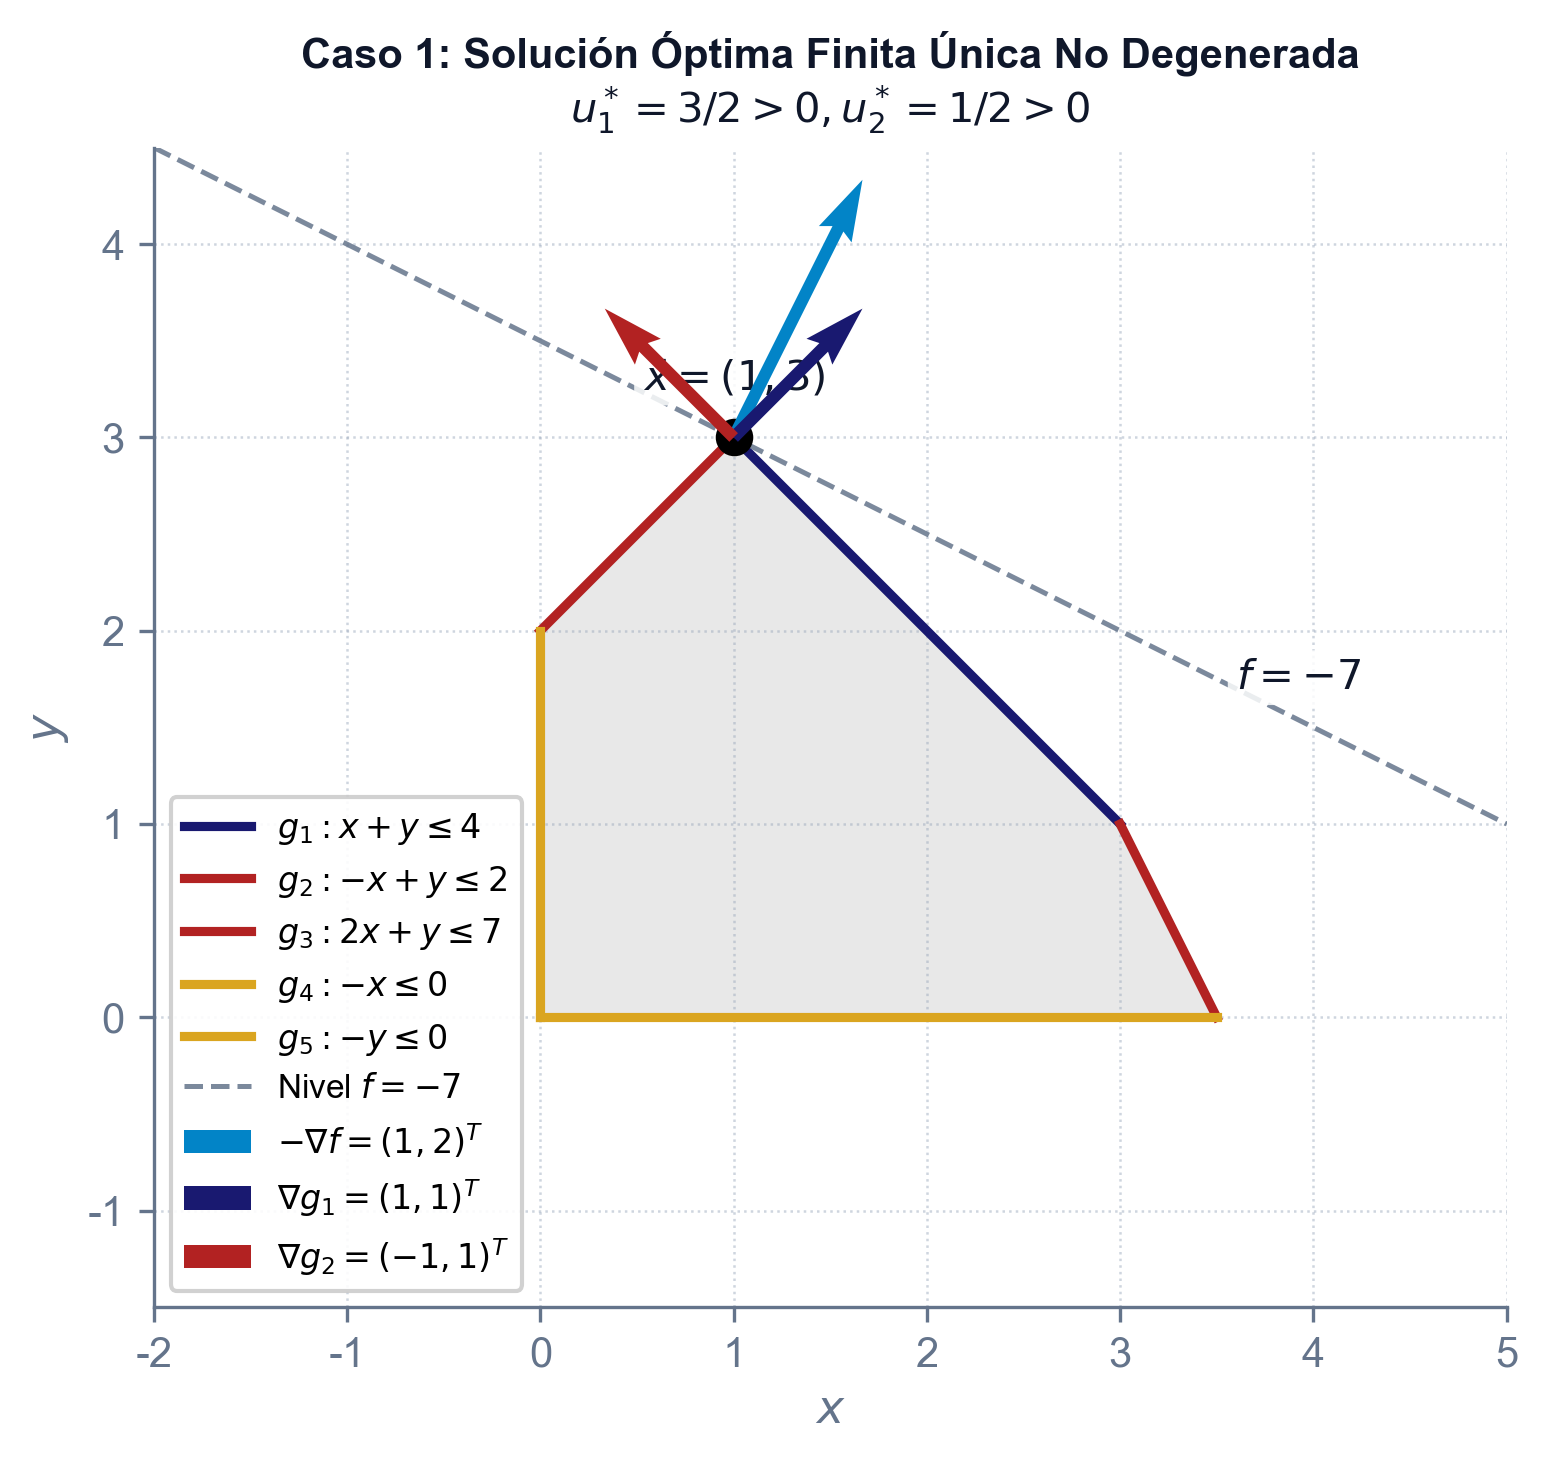
\includegraphics[width=0.75\linewidth,height=\textheight,keepaspectratio]{images/lp_caso1_unica_no_deg.png}

}

\caption{\label{fig-lp-caso1}Caso 1: Solución óptima finita única no
degenerada}

\end{figure}%

\textbf{Caso 2: El problema tiene solución óptima finita única
degenerada}

Se añade al problema anterior la restricción redundante
\(g_4(x, y) = y - 3 \le 0\): \[
\begin{aligned}
\min_{x, y \in \mathbb{R}} \quad & -x - 2y \\
\text{sujeto a} \quad & x + y - 4 \le 0 \quad (g_1) \\
& -x + y - 2 \le 0 \quad (g_2) \\
& 2x + y - 7 \le 0 \quad (g_3) \\
& y - 3 \le 0 \quad (g_4 \text{ redundante}) \\
& x, y \ge 0
\end{aligned}
\]

La solución óptima primal sigue siendo el vértice \((1,3)\) con valor
finito \(f(1,3) = -7\). Sin embargo, como muestra la
Figura~\ref{fig-lp-caso2}, en dicho punto coinciden tres restricciones
activas: \(g_1, g_2\) y \(g_4\). Al haber \(m = 3\) restricciones
activas para \(n = 2\) variables, el punto presenta sobredeterminación
geométrica. Los gradientes \(\nabla g_1 = (1,1)^T\),
\(\nabla g_2 = (-1,1)^T\) y \(\nabla g_4 = (0,1)^T\) no son linealmente
independientes (se rompe LICQ).

Aunque el punto satisface la condición de Fritz John (FJ), existen
múltiples combinaciones de multiplicadores para expresar \(-\nabla f\)
como combinación lineal no negativa de los gradientes activos. Cumplen
KKT tanto \(u = (u_1, u_2, u_4) = (3/2, 1/2, 0)\) como
\(u' = (u_1, u_2, u_4) = (1, 0, 1)\). Cualquier combinación convexa
\(\lambda u + (1-\lambda) u'\) (\(\forall \lambda \in [0,1]\)) es
también solución del dual. Por tanto, \textbf{el problema dual tiene
múltiples soluciones óptimas}.

\begin{figure}[H]

\centering{

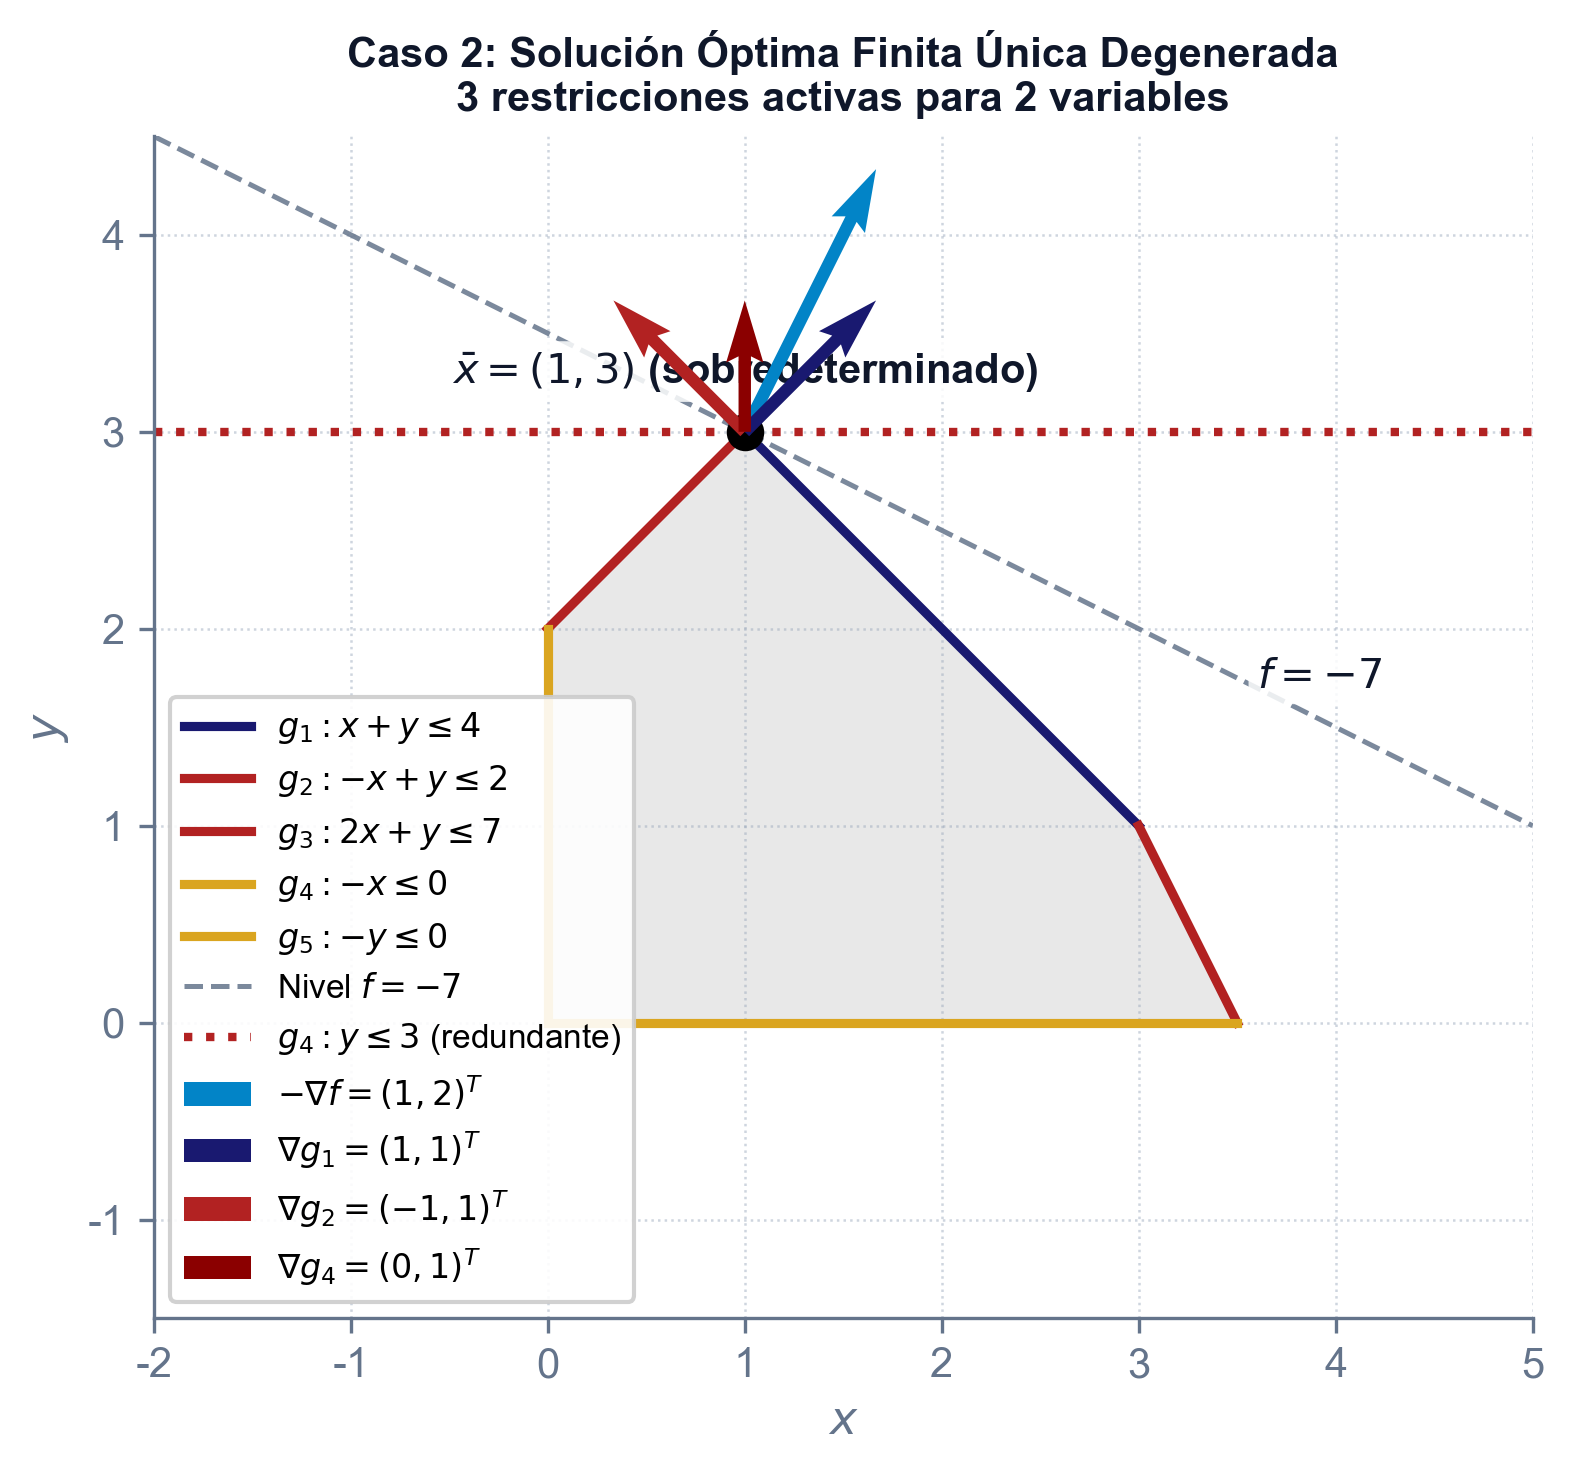
\includegraphics[width=0.75\linewidth,height=\textheight,keepaspectratio]{images/lp_caso2_unica_deg.png}

}

\caption{\label{fig-lp-caso2}Caso 2: Solución óptima finita única
degenerada}

\end{figure}%

\textbf{Caso 3: El problema tiene múltiples soluciones no degeneradas}

Se modifica la función objetivo a \(f(x, y) = -x - y\), manteniendo las
tres restricciones originales: \[
\begin{aligned}
\min_{x, y \in \mathbb{R}} \quad & -x - y \\
\text{sujeto a} \quad & x + y - 4 \le 0 \quad (g_1) \\
& -x + y - 2 \le 0 \quad (g_2) \\
& 2x + y - 7 \le 0 \quad (g_3) \\
& x, y \ge 0
\end{aligned}
\]

El vector opuesto de gradiente es \(-\nabla f = (1,1)^T\), paralelo al
gradiente de la restricción \(\nabla g_1 = (1,1)^T\). Como muestra la
Figura~\ref{fig-lp-caso3}, el conjunto de soluciones óptimas primales es
el segmento continuo entre \((1,3)\) y \((3,1)\). El problema primal
admite \textbf{múltiples soluciones óptimas finitas}.

En los puntos interiores de la arista óptima, la única restricción
activa es \(g_1\), siendo \(u_1^* = 1\) y el resto nulos. Al analizar
los vértices extremos: - En \((1,3)\): convergen \(g_1\) y \(g_2\), pero
el multiplicador asociado a \(g_2\) es nulo (\(u_2^* = 0\)). - En
\((3,1)\): convergen \(g_1\) y \(g_3\), pero el multiplicador asociado a
\(g_3\) es nulo (\(u_3^* = 0\)).

Por tanto, la solución del dual tendrá a lo sumo una variable no nula
(\(u_1 = 1\)), demostrando que \textbf{el problema dual tiene al menos
una solución degenerada}.

\begin{figure}[H]

\centering{

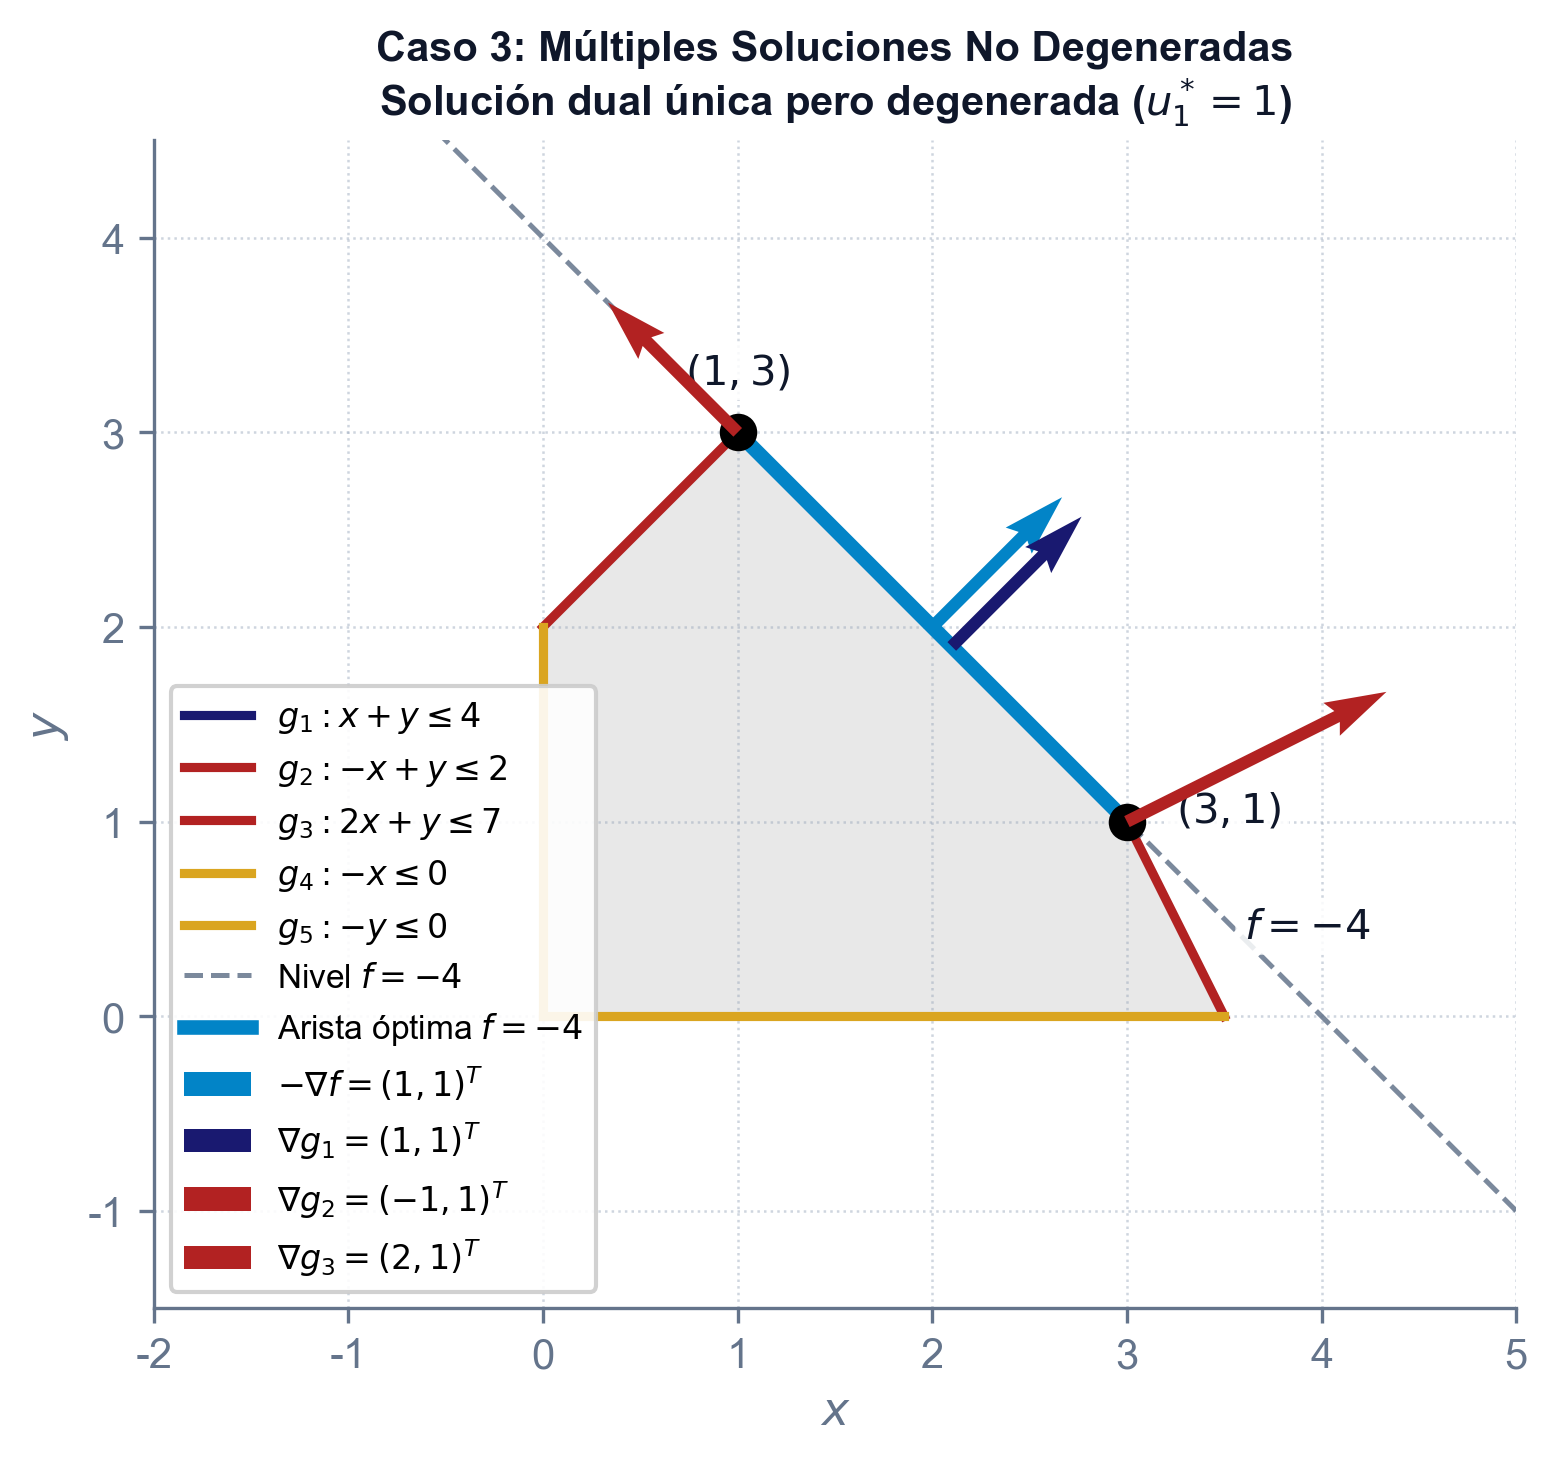
\includegraphics[width=0.75\linewidth,height=\textheight,keepaspectratio]{images/lp_caso3_multiples_no_deg.png}

}

\caption{\label{fig-lp-caso3}Caso 3: Múltiples soluciones no
degeneradas}

\end{figure}%

\textbf{Caso 4: El problema tiene múltiples soluciones y al menos una es
degenerada}

Se minimiza \(f(x, y) = -x - y\) incluyendo la restricción redundante
\(g_4(x, y) = y - 3 \le 0\): \[
\begin{aligned}
\min_{x, y \in \mathbb{R}} \quad & -x - y \\
\text{sujeto a} \quad & x + y - 4 \le 0 \quad (g_1) \\
& -x + y - 2 \le 0 \quad (g_2) \\
& 2x + y - 7 \le 0 \quad (g_3) \\
& y - 3 \le 0 \quad (g_4 \text{ redundante}) \\
& x, y \ge 0
\end{aligned}
\]

Como se ilustra geométricamente en la Figura~\ref{fig-lp-caso4a}, la
totalidad del segmento continuo entre los vértices \((1,3)\) y \((3,1)\)
constituye el conjunto de soluciones óptimas primales (todas las
combinaciones convexas de ambos vértices).

\begin{figure}[H]

\centering{

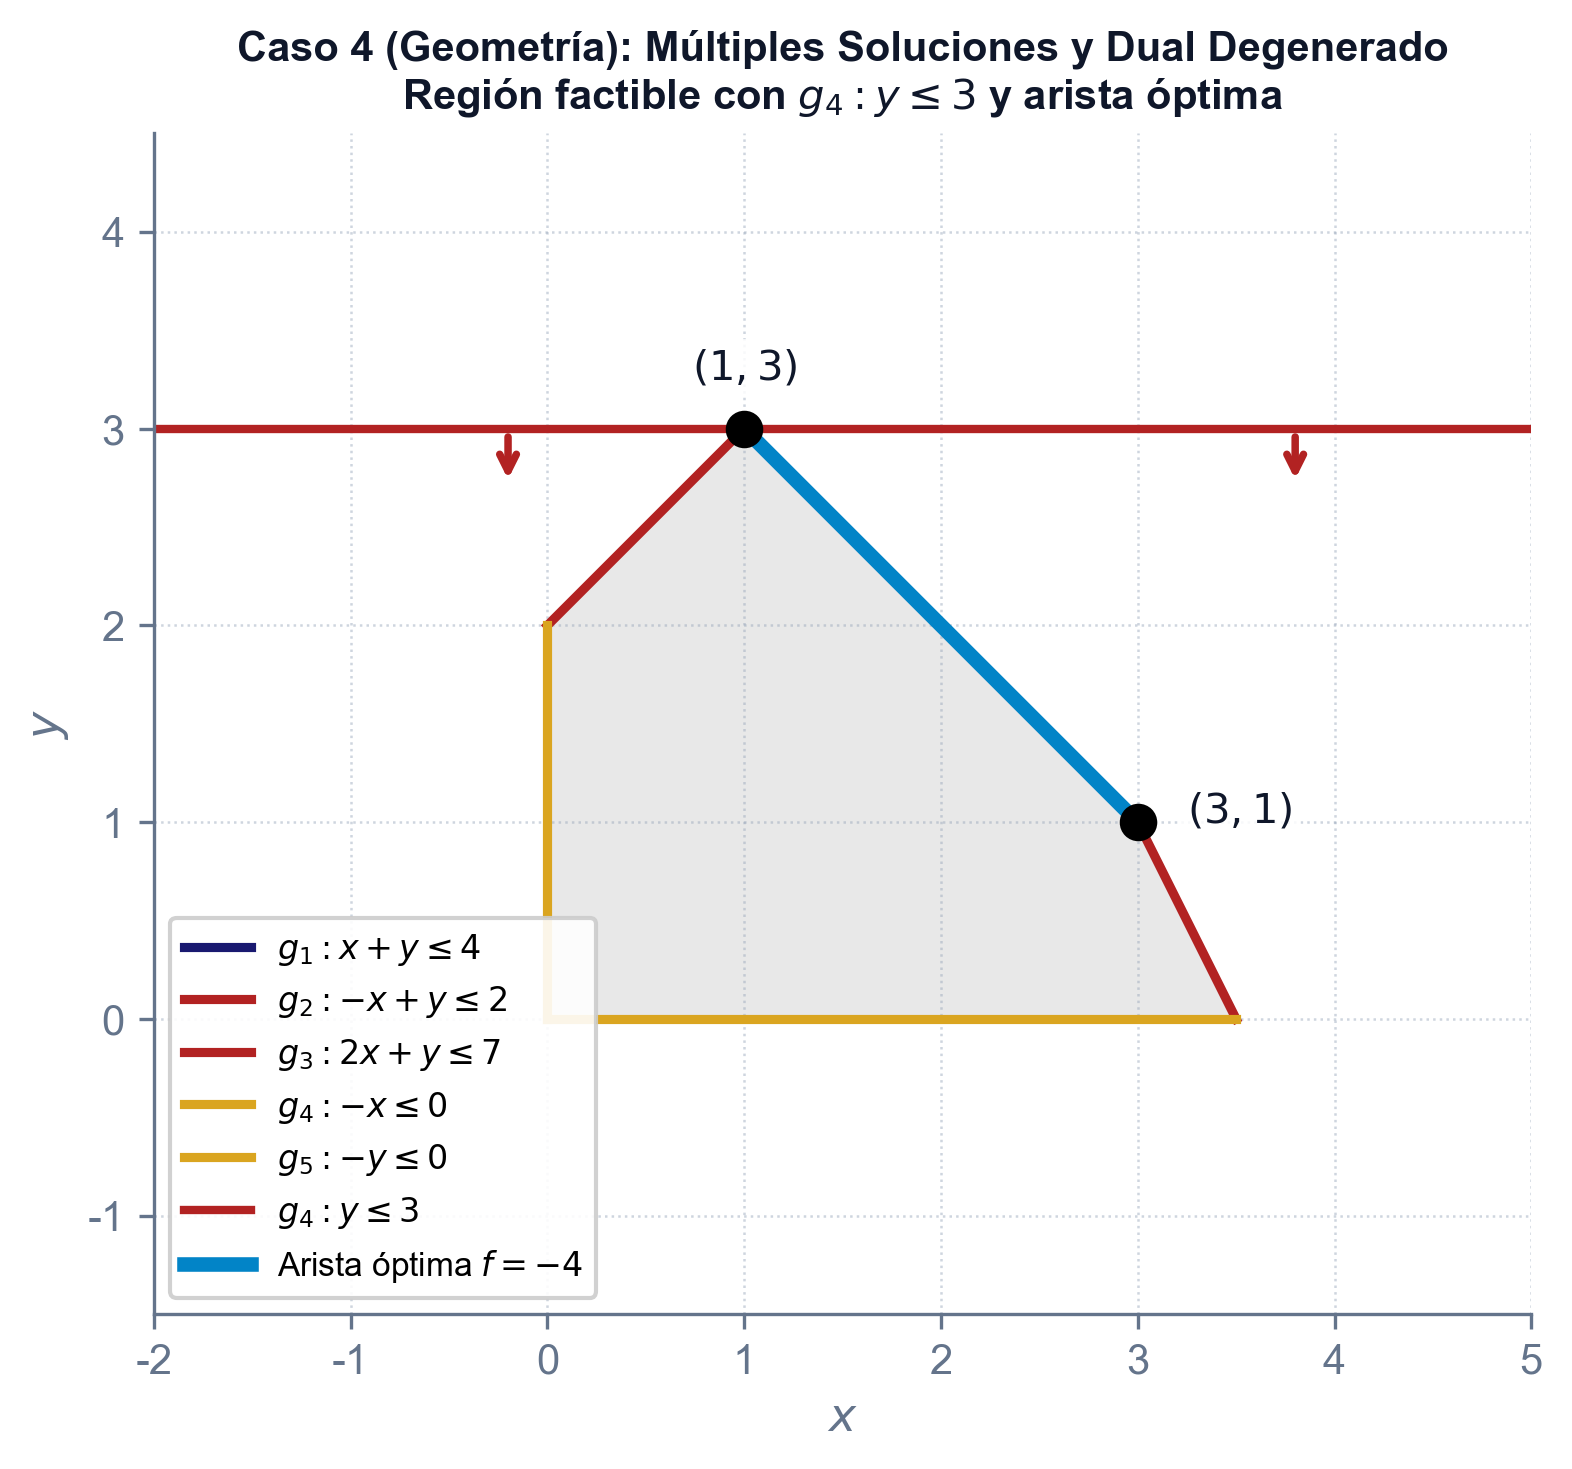
\includegraphics[width=0.75\linewidth,height=\textheight,keepaspectratio]{images/lp_caso4a_geometria.png}

}

\caption{\label{fig-lp-caso4a}Caso 4 (Geometría): Región factible con
arista óptima entre (1,3) y (3,1)}

\end{figure}%

Sin embargo, al analizar la estructura dual en la
Figura~\ref{fig-lp-caso4b}: - La solución del dual asociada al vértice
\((1,3)\) es \textbf{degenerada}, ya que en él convergen tres
restricciones activas (\(g_1, g_2, g_4\)), lo que genera
sobredeterminación geométrica y requiere dos multiplicadores nulos
(\(u_2 = 0\) y \(u_4 = 0\)). - Las soluciones asociadas a los puntos
interiores del segmento óptimo no son degeneradas, pues por hipótesis la
matriz de restricciones activas en el interior mantiene rango máximo.

Por tanto, como en el caso anterior, \textbf{el problema dual tiene
solución degenerada}, con la particularidad de que en el vértice
\((1,3)\) existen dos multiplicadores nulos (\(u_2\) y \(u_4\)).

\begin{figure}[H]

\centering{

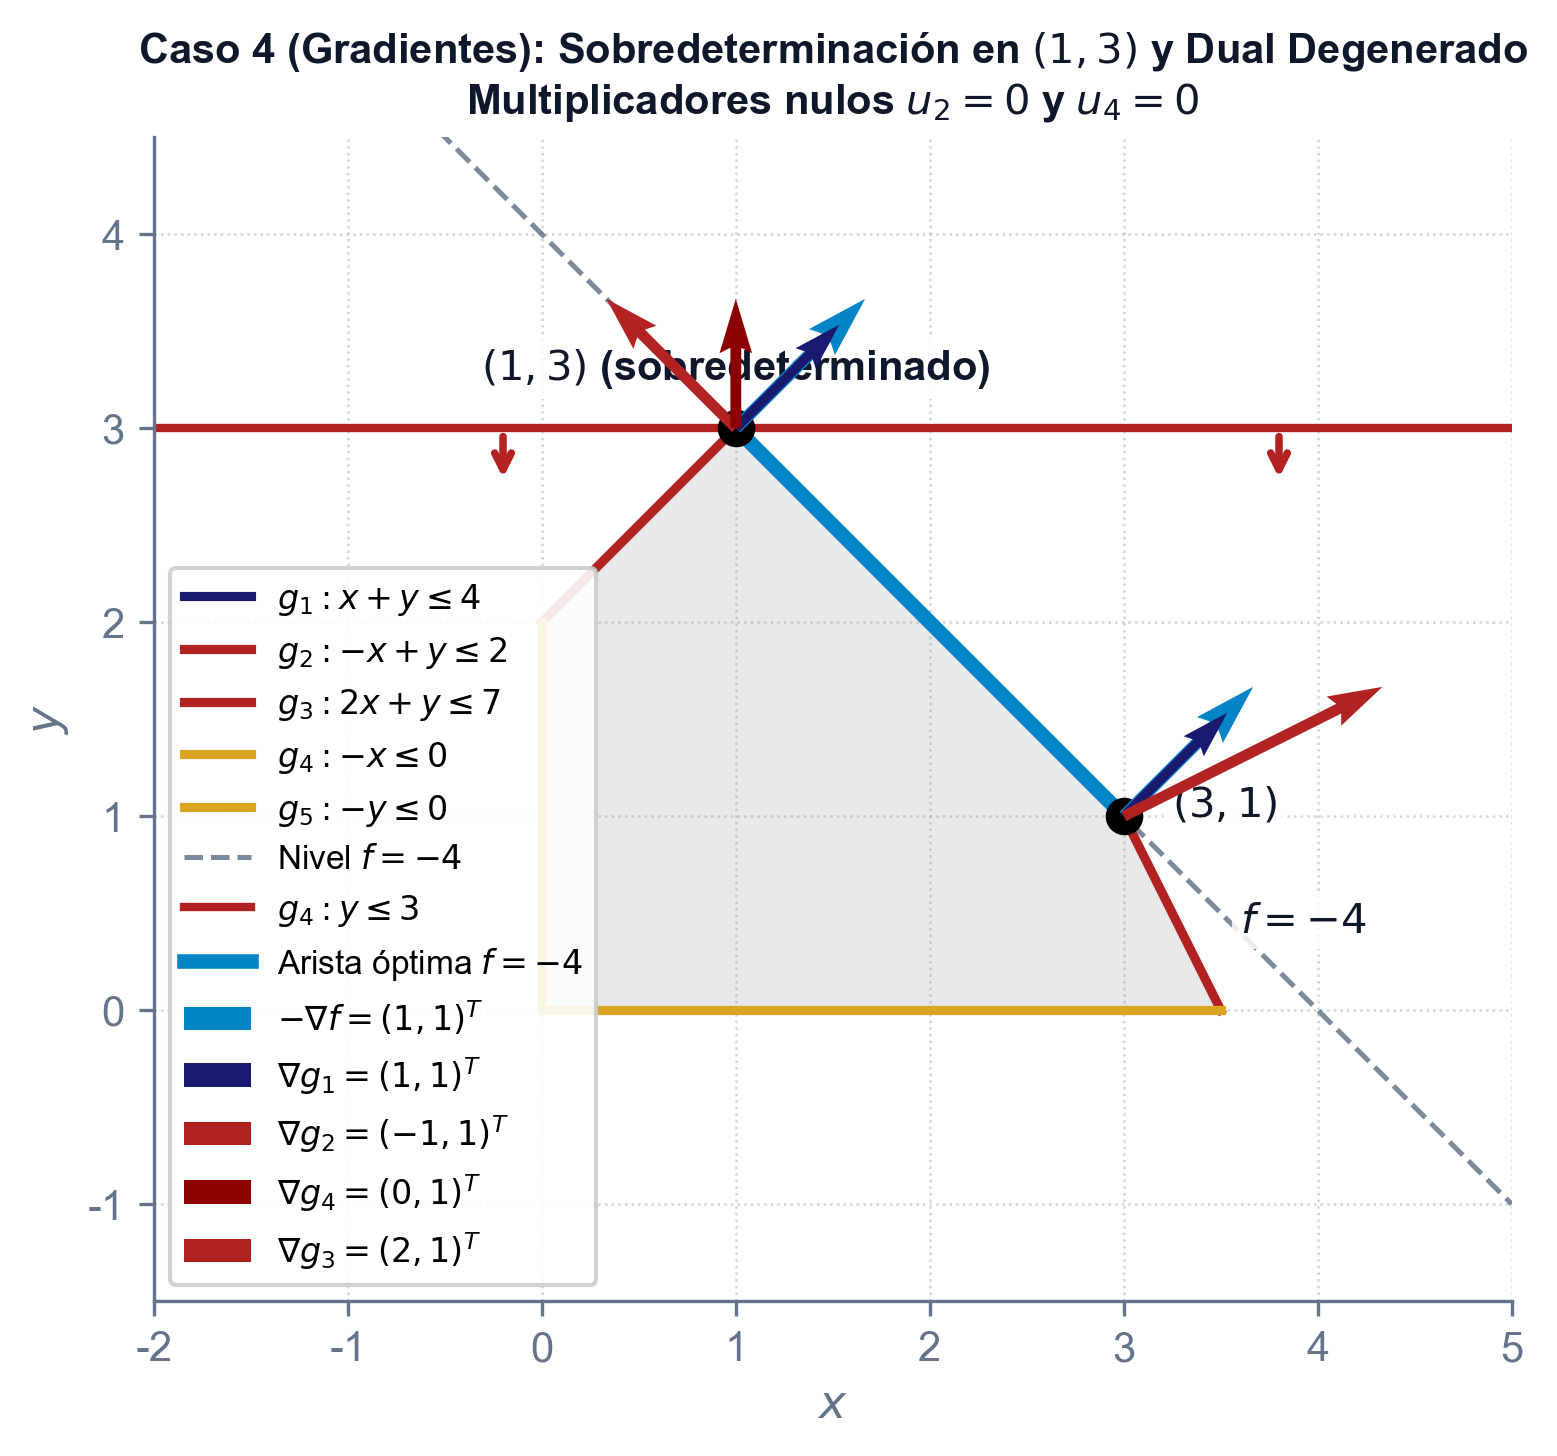
\includegraphics[width=0.75\linewidth,height=\textheight,keepaspectratio]{images/lp_caso4b_gradientes.png}

}

\caption{\label{fig-lp-caso4b}Caso 4 (Gradientes): Sobredeterminación en
(1,3) y multiplicadores nulos duales}

\end{figure}%

\textbf{Caso 5: El problema tiene solución no acotada}

Se elimina la restricción superior \(g_1\): \[
\begin{aligned}
\min_{x, y \in \mathbb{R}} \quad & -x - y \\
\text{sujeto a} \quad & -x + y - 2 \le 0 \quad (g_2) \\
& 2x + y - 7 \le 0 \quad (g_3) \\
& x, y \ge 0
\end{aligned}
\]

El valor objetivo decrece hacia \(-\infty\) sobre un rayo de recesión.
Ningún punto verifica las condiciones KKT. Por tanto, como muestra la
Figura~\ref{fig-lp-caso5}, \textbf{el problema dual no tiene solución
(es no factible)}.

\begin{figure}[H]

\centering{

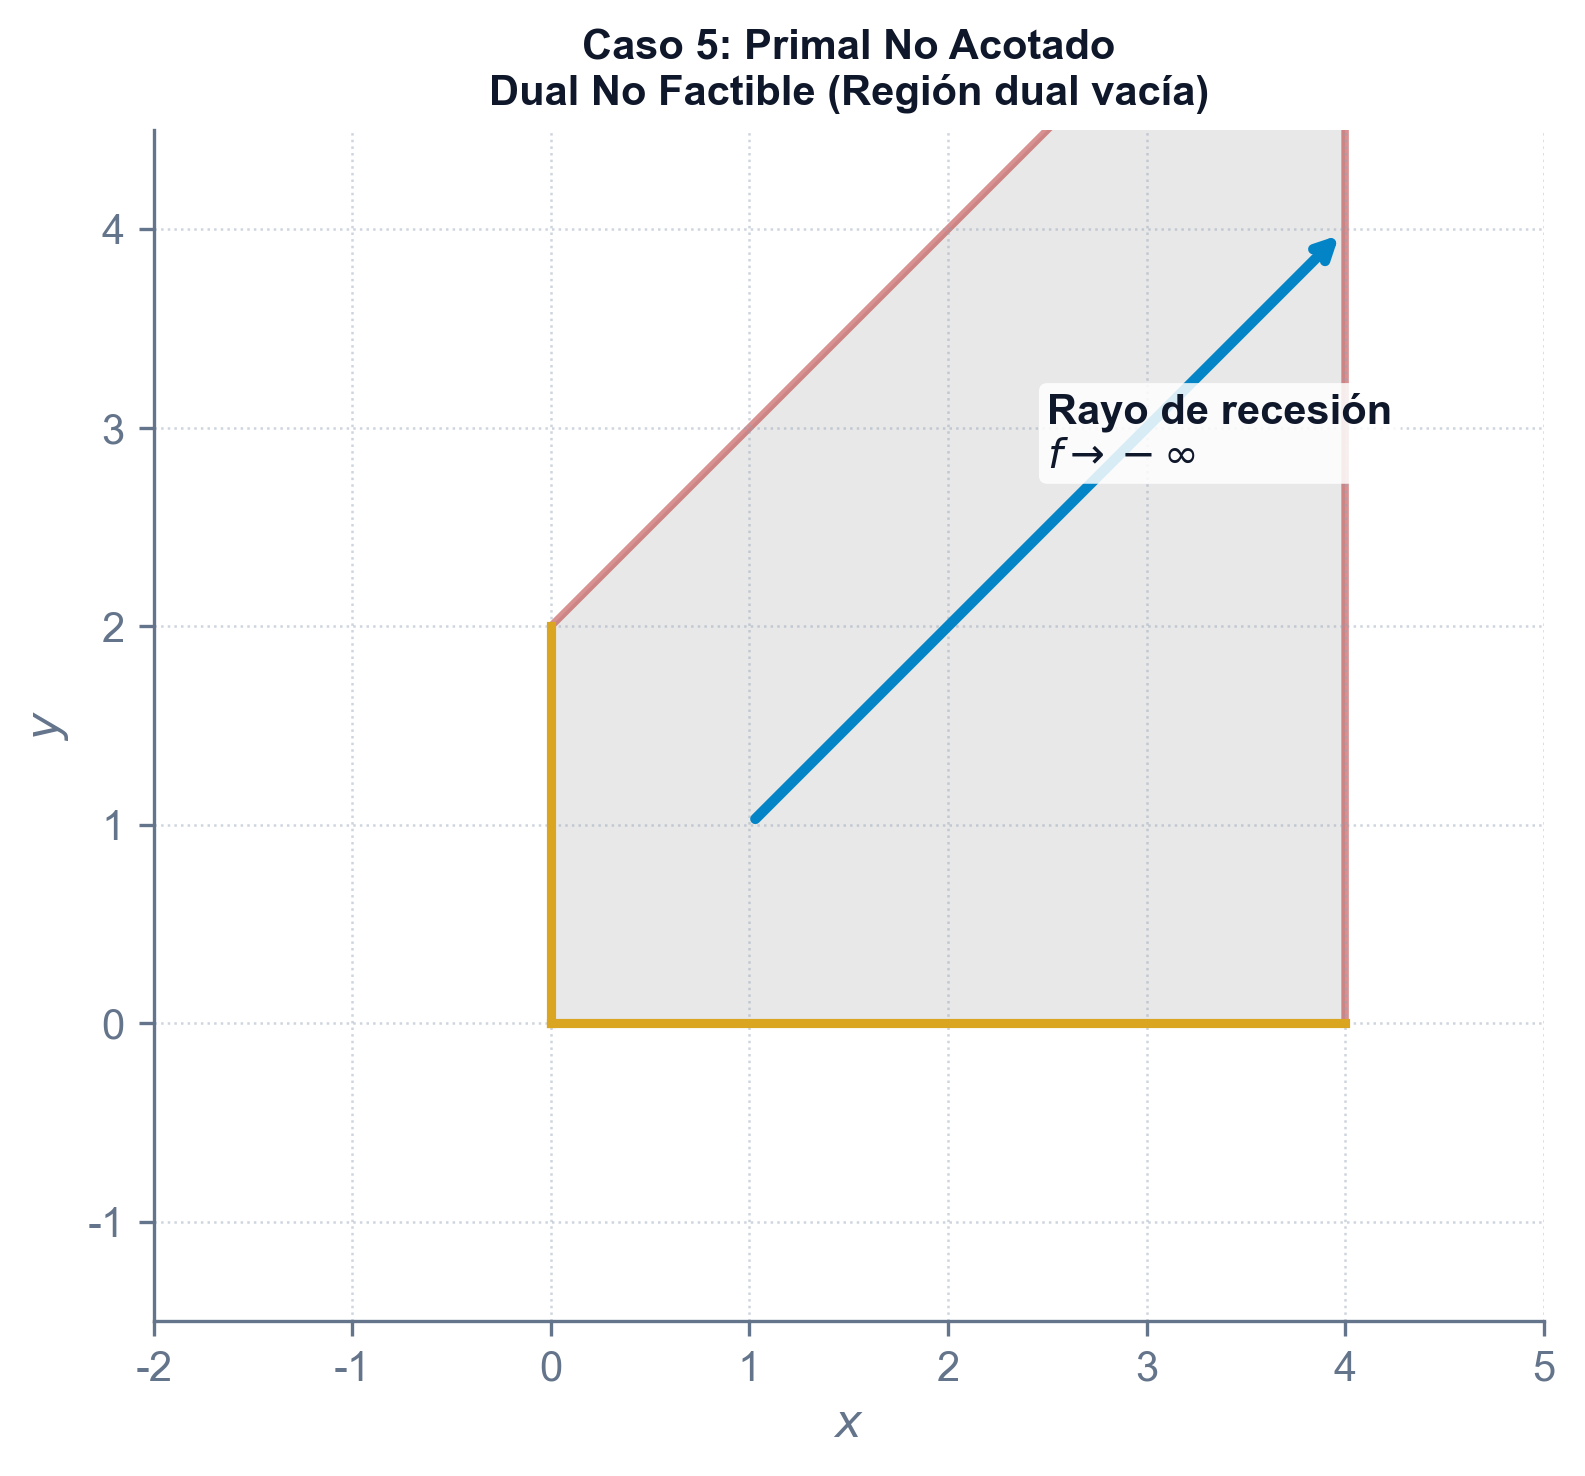
\includegraphics[width=0.75\linewidth,height=\textheight,keepaspectratio]{images/lp_caso5_no_acotado.png}

}

\caption{\label{fig-lp-caso5}Caso 5: Primal no acotado}

\end{figure}%

\textbf{Caso 6: El problema es no factible}

Se definen restricciones contradictorias que generan una región vacía:
\[
\begin{aligned}
\min_{x, y \in \mathbb{R}} \quad & -x - 2y \\
\text{sujeto a} \quad & x + y - 1 \le 0 \\
& -x - y + 3.5 \le 0 \\
& x, y \ge 0
\end{aligned}
\]

La región factible primal es vacía (Figura~\ref{fig-lp-caso6}).
Aplicando KKT al dual, este no puede poseer solución óptima finita,
concluyendo que \textbf{el problema dual es no factible o tiene solución
no acotada}.

\begin{figure}[H]

\centering{

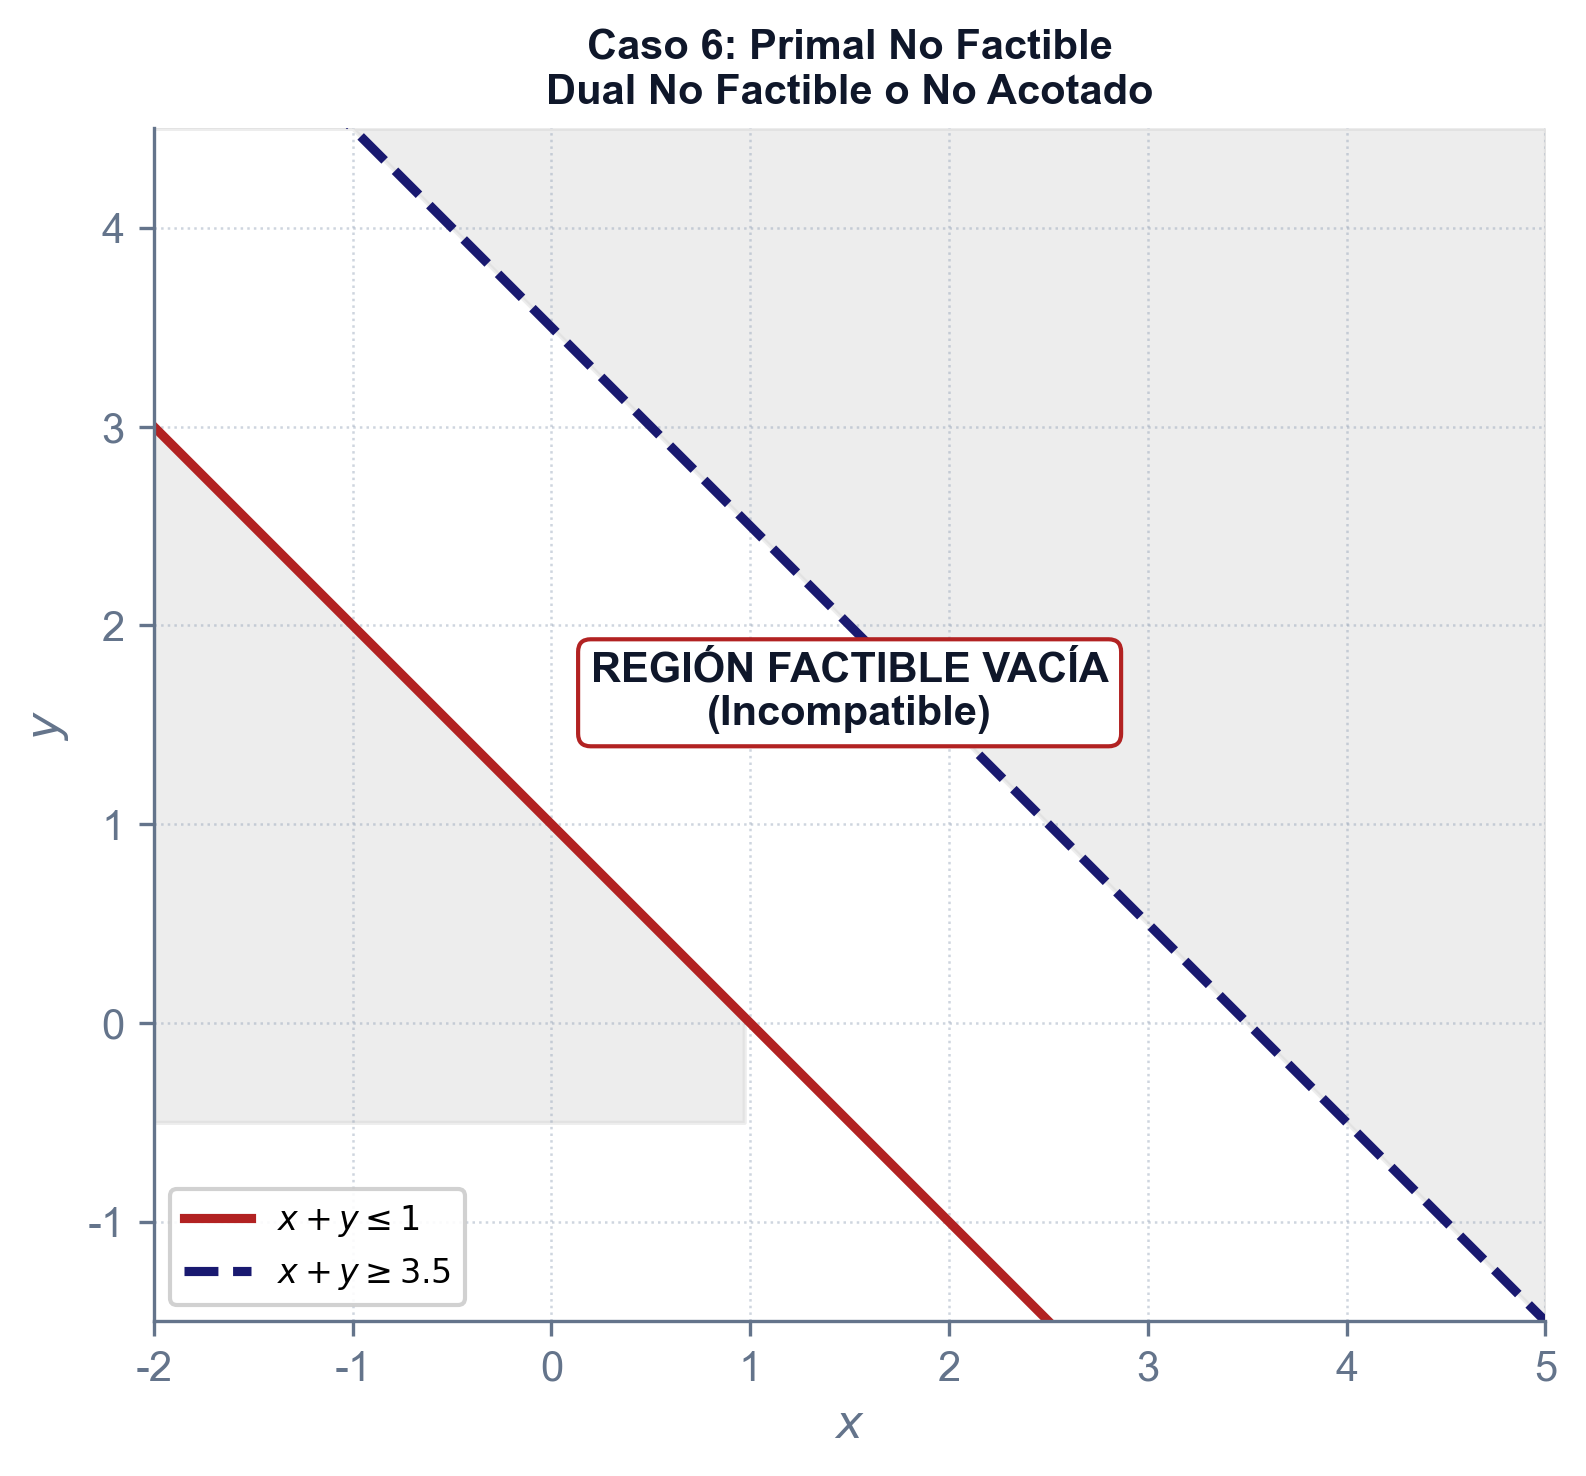
\includegraphics[width=0.75\linewidth,height=\textheight,keepaspectratio]{images/lp_caso6_no_factible.png}

}

\caption{\label{fig-lp-caso6}Caso 6: Primal no factible}

\end{figure}%

\end{tcolorbox}

En síntesis, el análisis geométrico y analítico por casos permite
establecer las siguientes relaciones de equivalencia fundamentales entre
las propiedades del problema primal y de su correspondiente problema
dual:

\begin{itemize}
\tightlist
\item
  Si el problema primal posee una solución óptima finita \textbf{única y
  degenerada}, entonces el problema dual posee \textbf{múltiples
  soluciones óptimas}.
\item
  Si el problema primal posee \textbf{múltiples soluciones óptimas},
  entonces el problema dual posee una solución óptima
  \textbf{degenerada}.
\end{itemize}

Dado que la dualidad en programación lineal constituye una propiedad
involutiva (el problema dual del dual coincide algebraicamente con el
primal original), se obtiene el resultado recíproco de caracterización
global:

\begin{tcolorbox}[enhanced jigsaw, toprule=.15mm, opacitybacktitle=0.6, coltitle=black, colbacktitle=quarto-callout-note-color!10!white, title=\textcolor{quarto-callout-note-color}{\faInfo}\hspace{0.5em}{Proposición: Equivalencia de dualidad entre degeneración y múltiples
óptimos}, arc=.35mm, rightrule=.15mm, toptitle=1mm, breakable, bottomtitle=1mm, titlerule=0mm, colback=white, opacityback=0, leftrule=.75mm, colframe=quarto-callout-note-color-frame, left=2mm, bottomrule=.15mm]

Dado un problema de optimización lineal y su correspondiente problema
dual asociado, uno de los dos problemas posee una solución óptima finita
\textbf{degenerada} si y solo si el otro problema posee
\textbf{múltiples puntos óptimos}.

\end{tcolorbox}

La siguiente tabla sintetiza la matriz de correspondencia completa entre
los escenarios de optimalidad y existencialidad del problema primal y
del problema dual:

\begin{longtable}[]{@{}ll@{}}
\toprule\noalign{}
Estado del Problema Primal & Estado del Problema Dual Asociado \\
\midrule\noalign{}
\endhead
\bottomrule\noalign{}
\endlastfoot
\textbf{Óptimo Único No Degenerado} & Óptimo Único No Degenerado \\
\textbf{Óptimo Único Degenerado} & Múltiples Soluciones Óptimas \\
\textbf{Múltiples Soluciones Óptimas} & Óptimo Único Degenerado \\
\textbf{No Acotado (\(f \to -\infty\))} & No Factible (Región Dual
Vacía) \\
\textbf{No Factible (Región Primal Vacía)} & No Factible o No Acotado \\
\end{longtable}

\section{Programación cuadrática
(QP)}\label{programaciuxf3n-cuadruxe1tica-qp}

La \textbf{Programación Cuadrática} (QP, por sus siglas en inglés,
\emph{Quadratic Programming}) constituye una clase fundamental de
optimización no lineal donde la función objetivo es una expresión de
segundo grado (cuadrática) y las restricciones que delimitan la región
factible son estrictamente afines o lineales de igualdad y desigualdad.

Consideremos el modelo estándar general de optimización cuadrática,
habitualmente denotado por (C):

\[
\begin{aligned}
\min_{x \in \mathbb{R}^n} \quad & f(x) = c^T x + \frac{1}{2} x^T Q x \\
\text{sujeto a} \quad & A x \ge b \\
& x \ge 0
\end{aligned}
\tag{C}
\]

donde \(x \in \mathbb{R}^n\) es el vector de variables de decisión,
\(c \in \mathbb{R}^n\) representa el vector de costes lineales,
\(Q \in \mathbb{R}^{n \times n}\) es una matriz cuadrada simétrica
(\(Q = Q^T\)) que recoge los coeficientes cuadráticos y las
interacciones cruzadas entre variables,
\(A \in \mathbb{R}^{m \times n}\) es la matriz de coeficientes de las
\(m\) restricciones, y \(b \in \mathbb{R}^m\) es el vector de términos
independientes o términos independientes. La región factible
\(S = \{x \in \mathbb{R}^n : A x \ge b, \ x \ge 0\}\) viene dada por la
intersección finita de semiespacios cerrados, constituyendo por tanto un
conjunto \textbf{convexo y poliédrico}.

\begin{tcolorbox}[enhanced jigsaw, toprule=.15mm, opacitybacktitle=0.6, coltitle=black, colbacktitle=quarto-callout-note-color!10!white, title=\textcolor{quarto-callout-note-color}{\faInfo}\hspace{0.5em}{Observación: Interpretación geométrica de la función objetivo cuadrática}, arc=.35mm, rightrule=.15mm, toptitle=1mm, breakable, bottomtitle=1mm, titlerule=0mm, colback=white, opacityback=0, leftrule=.75mm, colframe=quarto-callout-note-color-frame, left=2mm, bottomrule=.15mm]

Cuando la matriz \(Q\) es definida positiva (\(Q \succ 0\)), la función
cuadrática \(f(x)\) posee un único mínimo libre no restringido en
\(x^0 = -Q^{-1} c\). Sus curvas de nivel \(f(x) = k\) forman elipsoides
concéntricos centrados en \(x^0\). Desde una perspectiva geométrica,
resolver el problema (C) equivale a encontrar el punto del poliedro
factible \(S\) más cercano a \(x^0\) según la métrica inducida por la
matriz \(Q\).

\end{tcolorbox}

\subsection{Derivación formal del sistema
KKT}\label{derivaciuxf3n-formal-del-sistema-kkt}

Para obtener las condiciones KKT del modelo (C), reescribimos en primer
lugar las restricciones en la forma canónica \(\le 0\): \[
b - A x \le 0, \quad -x \le 0
\]

Asociamos a las \(m\) restricciones generales de desigualdad
\(A x \ge b\) un vector de multiplicadores duales
\(u = (u_1, \dots, u_m)^T \ge 0\), y a las \(n\) restricciones de no
negatividad de las variables \(x \ge 0\) un vector de multiplicadores de
holgura duales \(v = (v_1, \dots, v_n)^T \ge 0\). La función Lagrangiana
extendida del problema adopta la forma:

\[
L(x, u, v) = c^T x + \frac{1}{2} x^T Q x + u^T (b - A x) - v^T x
\]

Derivando parcialmente la Lagrangiana con respecto al vector primal
\(x\) e imponiendo el sistema completo de estacionariedad, factibilidad
y holgura complementaria, se obtiene el sistema KKT formal estructurado
en tres bloques fundamentales:

\begin{enumerate}
\def\labelenumi{\arabic{enumi}.}
\tightlist
\item
  \textbf{Condiciones de factibilidad primal}:

  \begin{itemize}
  \tightlist
  \item
    \textbf{Factibilidad de las restricciones afines generales
    (\(b - A x \le 0\))}: Exige que la solución \(x\) satisfaga
    simultáneamente la totalidad de las \(m\) restricciones generales de
    desigualdad \(A x \ge b\).
  \item
    \textbf{Factibilidad de no negatividad de las variables
    (\(x \ge 0\))}: Garantiza que el vector de variables de decisión
    \(x \in \mathbb{R}^n\) pertenezca al ortante no negativo.
  \end{itemize}
\item
  \textbf{Condiciones de factibilidad dual y estacionariedad}:

  \begin{itemize}
  \tightlist
  \item
    \textbf{Estacionariedad de la función Lagrangiana
    (\(\nabla_x L(x, u, v) = c + Q x - A^T u - v = 0\))}: Representa el
    equilibrio vectorial en el punto óptimo. Esta ecuación de
    factibilidad dual establece que el gradiente de la función objetivo
    cuadrática, \(\nabla f(x) = c + Q x\), debe poder expresarse como
    combinación lineal no negativa de los gradientes de las
    restricciones activas, \(A^T u + v\).
  \item
    \textbf{No negatividad de los multiplicadores duales
    (\(u \ge 0, v \ge 0\))}: Asegura que los multiplicadores duales
    \(u \in \mathbb{R}^m\) asociados a las restricciones generales de
    desigualdad y \(v \in \mathbb{R}^n\) asociados a las barreras de no
    negatividad orienten los vectores normales en sentido opuesto a las
    direcciones de descenso.
  \end{itemize}
\item
  \textbf{Condiciones de holgura complementaria}:

  \begin{itemize}
  \tightlist
  \item
    \textbf{Complementariedad de las restricciones generales
    (\(u_i (b_i - a^i x) = 0, \forall i = 1, \dots, m\))}: Establece que
    si una restricción general es inactiva (\(b_i - a^i x < 0\)), su
    multiplicador dual o precio sombra asociado debe ser nulo
    (\(u_i = 0\)). Recíprocamente, si el multiplicador es estrictamente
    positivo (\(u_i > 0\)), la restricción debe verificarse como
    igualdad estricta (\(a^i x = b_i\)).
  \item
    \textbf{Complementariedad de no negatividad
    (\(v_i x_i = 0, \forall i = 1, \dots, n\))}: Garantiza que si una
    variable de decisión es positiva (\(x_i > 0\)), su holgura dual
    asociada debe anularse (\(v_i = 0\)), mientras que si la variable se
    ubica en su límite inferior (\(x_i = 0\)), la holgura dual
    \(v_i \ge 0\) puede tomar valores positivos.
  \end{itemize}
\end{enumerate}

donde \(a^i\) denota la fila \(i\)-ésima de la matriz de coeficientes
\(A\).

Cuando la función objetivo \(f(x)\) es convexa (propiedad que se
verifica si y solo si la matriz \(Q\) es \textbf{semidefinida positiva},
\(Q \succeq 0\), es decir, \(x^T Q x \ge 0\) para todo
\(x \in \mathbb{R}^n\)), las condiciones necesarias de
Karush-Kuhn-Tucker resultan también \textbf{suficientes} para certificar
la optimalidad global.

\begin{tcolorbox}[enhanced jigsaw, toprule=.15mm, opacitybacktitle=0.6, coltitle=black, colbacktitle=quarto-callout-note-color!10!white, title=\textcolor{quarto-callout-note-color}{\faInfo}\hspace{0.5em}{Proposición: Suficiencia de las condiciones KKT en QP convexa}, arc=.35mm, rightrule=.15mm, toptitle=1mm, breakable, bottomtitle=1mm, titlerule=0mm, colback=white, opacityback=0, leftrule=.75mm, colframe=quarto-callout-note-color-frame, left=2mm, bottomrule=.15mm]

Si la matriz de términos cuadráticos \(Q\) es semidefinida positiva
(\(Q \succeq 0\)), el problema de programación cuadrática (C) es
convexo. En consecuencia, \textbf{cualquier solución que satisfaga el
sistema de condiciones KKT es una solución óptima global del problema
(C)}.

\end{tcolorbox}

Sin embargo, si la convexidad no se satisface, el panorama analítico
cambia sustancialmente:

\begin{tcolorbox}[enhanced jigsaw, toprule=.15mm, opacitybacktitle=0.6, coltitle=black, colbacktitle=quarto-callout-warning-color!10!white, title=\textcolor{quarto-callout-warning-color}{\faExclamationTriangle}\hspace{0.5em}{Advertencia: Importancia crítica de la convexidad (\(Q \succeq 0\))}, arc=.35mm, rightrule=.15mm, toptitle=1mm, breakable, bottomtitle=1mm, titlerule=0mm, colback=white, opacityback=0, leftrule=.75mm, colframe=quarto-callout-warning-color-frame, left=2mm, bottomrule=.15mm]

Si la matriz \(Q\) no es semidefinida positiva (posee autovalores
estrictamente negativos), el problema cuadrático deja de ser convexo. En
tal escenario, las condiciones KKT son únicamente necesarias pero no
suficientes, pudiendo caracterizar máximos locales o puntos de silla, y
los algoritmos basados en pivotes lineales como el de Wolfe no
garantizan la convergencia al óptimo global.

\end{tcolorbox}

\subsection{Transformación mediante variables de holgura y linealidad
del
sistema}\label{transformaciuxf3n-mediante-variables-de-holgura-y-linealidad-del-sistema}

Para transformar las desigualdades primales \(b - A x \le 0\) en
ecuaciones lineales manejables algebraicamente por algoritmos de pivote,
introducimos un vector de \textbf{variables primales de holgura} no
negativas \(y = (y_1, \dots, y_m)^T \ge 0\). De este modo:

\[
b - A x \le 0 \iff b - A x + y = 0, \quad \text{con } y \ge 0
\]

Analíticamente, se verifica la equivalencia directa entre el exceso de
la restricción y el valor de la variable de holgura:

\[
b_i - a^i x < 0 \iff y_i > 0, \quad \forall i = 1, \dots, m
\]

Sustituyendo esta relación en la primera condición de holgura
complementaria, el producto escalar \(u_i (b_i - a^i x) = 0\) equivale a
la condición de ortogonalidad escalar:

\[
u_i y_i = 0, \quad \forall i = 1, \dots, m
\]

Dado que todas las variables del sistema son estrictamente no negativas
(\(u, v, x, y \ge 0\)), la anulación de cada producto individual
\(u_i y_i = 0\) y \(v_i x_i = 0\) para todo \(i\) equivale a exigir que
la suma de sus productos escalares se anule globalmente:

\[
\begin{cases}
u_i y_i = 0, & \forall i = 1, \dots, m \\
v_i x_i = 0, & \forall i = 1, \dots, n
\end{cases}
\iff \sum_{i=1}^m u_i y_i + \sum_{i=1}^n v_i x_i = 0 \iff u^T y + v^T x = 0
\]

Agrupando el conjunto de relaciones obtenidas, el sistema KKT de la
programación cuadrática convexa (C) se expresa inicialmente en la
siguiente forma algebraica estandarizada:

\[
\begin{aligned}
b - A x + y &= 0 \\
c + Q x - A^T u - v &= 0 \\
x, y, u, v &\ge 0 \\
u^T y + v^T x &= 0
\end{aligned}
\]

Este planteamiento formal revela una propiedad matemática fundamental
para la resolución computacional: excepto por el último conjunto de
restricciones no lineal de holgura complementaria
(\(u^T y + v^T x = 0\)), todo el resto del sistema de ecuaciones
(factibilidad primal \(b - A x + y = 0\) y estacionariedad
\(c + Q x - A^T u - v = 0\)) es \textbf{estrictamente lineal}.

\subsection{Algoritmo del Símplex de Wolfe con regla de entrada
restringida}\label{algoritmo-del-suxedmplex-de-wolfe-con-regla-de-entrada-restringida}

Como consecuencia de esta estructura parcialmente lineal, es posible
resolver el sistema KKT (y, por tanto, hallar la solución óptima del
problema cuadrático convexo C) adaptando las operaciones matriciales de
pivote del algoritmo del Símplex lineal.

Para lograr este objetivo, se siguen los siguientes tres pasos:

\begin{enumerate}
\def\labelenumi{\arabic{enumi}.}
\tightlist
\item
  \textbf{Se relaja la restricción de holgura complementaria}
  \(u^T y + v^T x = 0\).
\item
  \textbf{Se añaden variables artificiales} no negativas
  \(z = (z_1, \dots, z_n)^T \ge 0\) al conjunto de ecuaciones de
  estacionariedad (Factibilidad dual 1), obteniendo
  \(c + Q x - A^T u - v + z = 0\) con \(z \ge 0\).
\item
  \textbf{Se intenta que estas variables artificiales tomen el valor
  cero} resolviendo el siguiente problema de programación lineal
  auxiliar:
\end{enumerate}

\[
\begin{aligned}
\min \quad & \sum_{i=1}^n z_i \\
\text{sujeto a} \quad & b - A x + y = 0 \\
& c + Q x - A^T u - v + z = 0 \\
& x, y, u, v, z \ge 0
\end{aligned}
\]

Para garantizar que la solución del problema de programación lineal
auxiliar sea una solución válida y exacta del problema cuadrático
original (C), hay que modificar el criterio de selección de la variable
candidata a entrar en la base del Símplex aplicando la \textbf{regla de
entrada restringida} (\emph{restricted entry rule}) de Wolfe:

\begin{itemize}
\tightlist
\item
  \textbf{Regla de complementariedad primal-dual (\(u_i, y_i\))}: La
  variable multiplicadora dual \(u_i\) \textbf{no es candidata} a entrar
  en la base Símplex si su correspondiente variable de holgura primal
  \(y_i\) es básica (\(y_i \in \text{Base}\)), y viceversa.
\item
  \textbf{Regla de complementariedad de no negatividad (\(v_j, x_j\))}:
  La variable de holgura dual \(v_j\) \textbf{no es candidata} a entrar
  en la base Símplex si la correspondiente variable primal \(x_j\) es
  básica (\(x_j \in \text{Base}\)), y viceversa.
\end{itemize}

Al resolver el problema de programación lineal auxiliar bajo la regla de
entrada restringida, se obtienen los siguientes dos criterios de
caracterización global:

\begin{itemize}
\tightlist
\item
  \textbf{Si el valor óptimo de este problema es 0}
  (\(\min \sum z_i = 0\)), todas las variables artificiales han
  abandonado la base (\(z^* = 0\)). Como la regla de pivote restringido
  impide que variables complementarias formen parte de la base
  simultáneamente, la solución básica resultante satisface la
  complementariedad \(u^{*T} y^* + v^{*T} x^* = 0\), por lo que el
  vector \(x^*\) \textbf{es la solución óptima para (C)}.
\item
  \textbf{Por el contrario, si es estrictamente positivo}
  (\(\min \sum z_i > 0\)), resulta imposible reducir las variables
  artificiales a cero respetando la regla de entrada restringida. En tal
  caso, la condición de complementariedad no puede satisfacerse de forma
  simultánea con la factibilidad, por lo que \textbf{el problema (C) NO
  tiene solución} (es no factible).
\end{itemize}

\begin{tcolorbox}[enhanced jigsaw, toprule=.15mm, opacitybacktitle=0.6, coltitle=black, colbacktitle=quarto-callout-note-color!10!white, title=\textcolor{quarto-callout-note-color}{\faInfo}\hspace{0.5em}{Nota: Garantía de convergencia finita del algoritmo de Wolfe}, arc=.35mm, rightrule=.15mm, toptitle=1mm, breakable, bottomtitle=1mm, titlerule=0mm, colback=white, opacityback=0, leftrule=.75mm, colframe=quarto-callout-note-color-frame, left=2mm, bottomrule=.15mm]

Puesto que el algoritmo del Símplex modificado por Wolfe opera sobre el
conjunto de soluciones básicas factibles del sistema de ecuaciones
lineales ampliado (el cual consta de un número finito de bases posibles)
y la función objetivo auxiliar \(\sum z_i\) decrece de manera monótona a
cada paso de pivote, se garantiza que el algoritmo finaliza en un número
finito de iteraciones.

\end{tcolorbox}

Para fijar los conceptos teóricos presentados y comprender de forma
intuitiva el funcionamiento algebraico y geométrico del algoritmo del
Símplex de Wolfe, a continuación se resuelve detalladamente un problema
completo de programación cuadrática convexa en dos dimensiones.

\begin{tcolorbox}[enhanced jigsaw, toprule=.15mm, opacitybacktitle=0.6, coltitle=black, colbacktitle=quarto-callout-tip-color!10!white, title=\textcolor{quarto-callout-tip-color}{\faLightbulb}\hspace{0.5em}{Ejemplo: Resolución completa mediante el algoritmo del símplex de Wolfe}, arc=.35mm, rightrule=.15mm, toptitle=1mm, breakable, bottomtitle=1mm, titlerule=0mm, colback=white, opacityback=0, leftrule=.75mm, colframe=quarto-callout-tip-color-frame, left=2mm, bottomrule=.15mm]

\textbf{Enunciado del problema}: Consideremos el problema de
optimización cuadrática en el que se busca minimizar la distancia
euclídea al cuadrado desde las variables \((x_1, x_2)\) al punto
objetivo \((4,4)\), sobre una región factible poliédrica
\(S \subset \mathbb{R}^2\):

\[
\begin{aligned}
\min_{x_1, x_2 \in \mathbb{R}} \quad & (x_1 - 4)^2 + (x_2 - 4)^2 \\
\text{sujeto a} \quad & x_1 + x_2 \le 4 \\
& -x_1 + x_2 \le 2 \\
& 2x_1 + x_2 \le 7 \\
& x_1, x_2 \ge 0
\end{aligned}
\qquad \equiv \qquad
\begin{aligned}
\min_{x_1, x_2 \in \mathbb{R}} \quad & (x_1 - 4)^2 + (x_2 - 4)^2 \\
\text{sujeto a} \quad & -4 + x_1 + x_2 \le 0 \\
& -2 - x_1 + x_2 \le 0 \\
& -7 + 2x_1 + x_2 \le 0 \\
& x_1, x_2 \ge 0
\end{aligned}
\]

\textbf{Formulación del problema auxiliar del Símplex de Wolfe}:
Identificamos la matriz cuadrática
\(Q = \begin{pmatrix} 2 & 0 \\ 0 & 2 \end{pmatrix}\) (estrictamente
definida positiva, garantizando la convexidad del problema), el vector
lineal \(c = (-8, -8)^T\), la matriz de coeficientes
\(A = \begin{pmatrix} -1 & -1 \\ 1 & -1 \\ -2 & -1 \end{pmatrix}\) y el
vector de términos independientes \(b = (-4, 2, -7)^T\).

Al introducir las variables primales de holgura \(y_1, y_2, y_3 \ge 0\),
los multiplicadores duales \(u_1, u_2, u_3 \ge 0\), las holguras duales
\(v_1, v_2 \ge 0\) y las variables artificiales \(z_1, z_2 \ge 0\), el
problema de programación lineal auxiliar a minimizar resulta:

\[
\begin{aligned}
\min \quad & z_1 + z_2 \\
\text{sujeto a} \quad & -4 + x_1 + x_2 + y_1 = 0 \\
& -2 - x_1 + x_2 + y_2 = 0 \\
& -7 + 2x_1 + x_2 + y_3 = 0 \\
& 2(x_1 - 4) + u_1 - u_2 + 2u_3 - v_1 + z_1 = 0 \\
& 2(x_2 - 4) + u_1 + u_2 + u_3 - v_2 + z_2 = 0 \\
& x_1, x_2, y_1, y_2, y_3, u_1, u_2, u_3, v_1, v_2, z_1, z_2 \ge 0
\end{aligned}
\]

reescribiendo las ecuaciones de estacionariedad como
\(2x_1 + u_1 - u_2 + 2u_3 - v_1 + z_1 = 8\) y
\(2x_2 + u_1 + u_2 + u_3 - v_2 + z_2 = 8\).

\textbf{Representación gráfica de la solución}: Como se ilustra
geométricamente en la Figura~\ref{fig-qp-ejemplo-geometria}, las curvas
de nivel de la función objetivo representan círculos concéntricos
centrados en el mínimo libre no restringido \((4,4)\). La solución
óptima del problema corresponde al punto de la región factible \(S\) más
próximo a \((4,4)\), alcanzándose la tangencia en el punto
\(\bar{x} = (2,2)\) con un valor objetivo de \(f(2,2) = 8\).

\begin{figure}[H]

\centering{

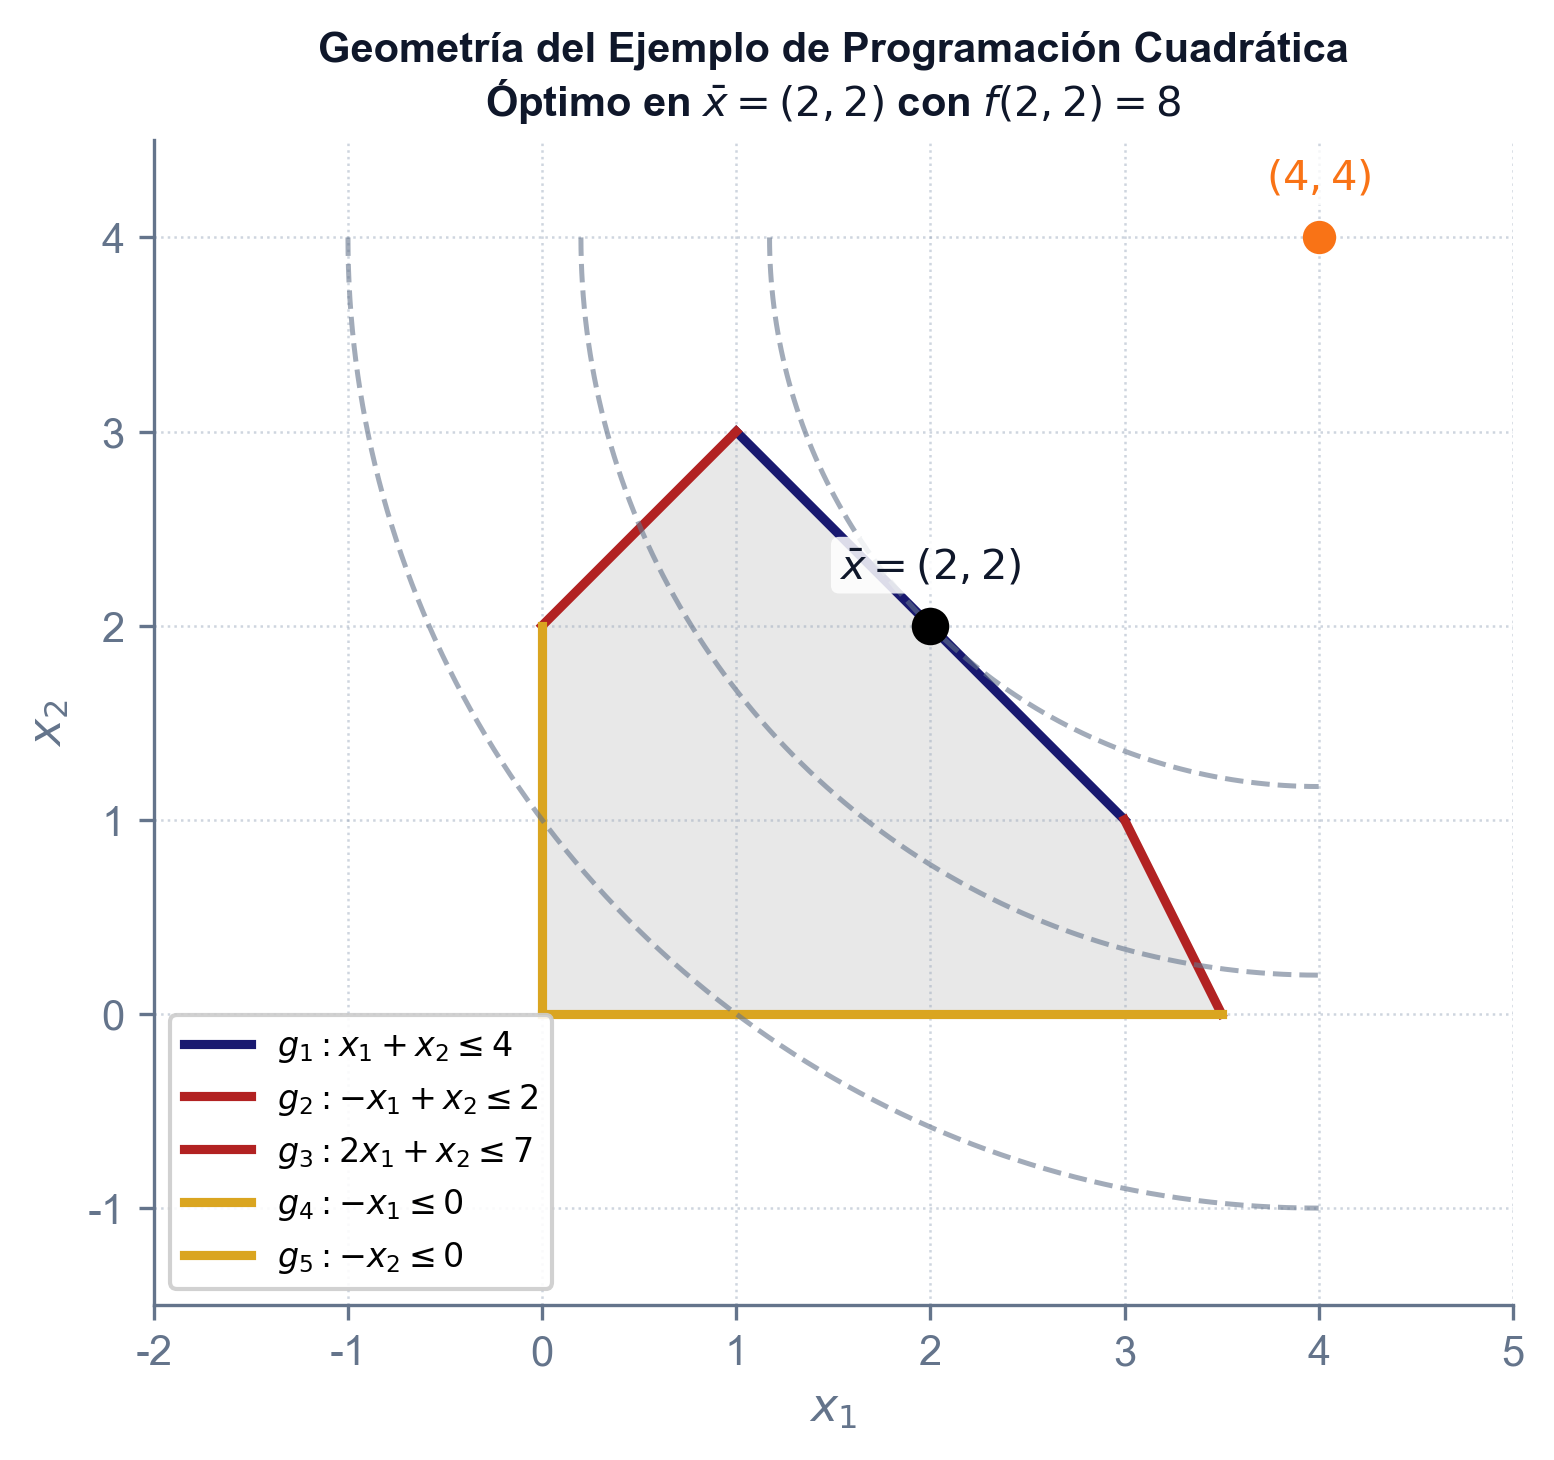
\includegraphics[width=0.75\linewidth,height=\textheight,keepaspectratio]{images/qp_ejemplo_geometria.png}

}

\caption{\label{fig-qp-ejemplo-geometria}Geometría de la región factible
y tangencia de la función objetivo cuadrática en el óptimo}

\end{figure}%

\textbf{Solución matemática del sistema KKT}: Al resolver el sistema
KKT, la solución exacta resultante para todas las variables primales,
duales, de holgura y artificiales es:

\[
\begin{aligned}
x_1^* &= 2, \quad x_2^* = 2 \\
u_1^* &= 4, \quad u_2^* = 0, \quad u_3^* = 0 \\
y_1^* &= 0, \quad y_2^* = 2, \quad y_3^* = 1 \\
v_1^* &= 0, \quad v_2^* = 0 \\
z_1^* &= 0, \quad z_2^* = 0
\end{aligned}
\]

\textbf{Resolución mediante el Algoritmo del Símplex de Wolfe (Tablas e
Interpretación Geométrica)}:

A continuación se detalla la progresión iterativa de las tablas del
Símplex y su correspondiente traslación geométrica sobre la región
factible a cada paso.

\textbf{Iteración 1 (Paso 1: Inicio en el Origen)}\\
En la primera iteración, la solución básica inicial parte con las
variables primales en el origen \(x_1=0, x_2=0\). Las variables primales
de holgura absorben los términos independientes
(\(y_1=4, y_2=2, y_3=7\)) y las variables artificiales toman el valor
\(z_1=8, z_2=8\), dando un coste artificial inicial de \(\sum z_i = 16\)
y un valor de la función objetivo de distancia \(f(0,0)=32\).

\begin{itemize}
\tightlist
\item
  \textbf{Base inicial}: \(\{y_1, y_2, y_3, z_1, z_2\}\),
  \textbf{Objetivo artificial}: \(z_1 + z_2 = 8 + 8 = 16\).
\item
  \textbf{Criterio de entrada}: Los costes reducidos negativos son
  \(x_1 (-2)\), \(x_2 (-2)\), \(u_1 (-2)\) y \(u_3 (-3)\).
\item
  \textbf{Regla de complementariedad dual}: Las variables \(u_1\) y
  \(u_3\) {están bloqueadas} porque sus variables primales asociadas
  \(y_1, y_3\) forman parte de la base actual.
\item
  \textbf{Pivote}: Seleccionamos la variable candidata
  {\(x_2 \downarrow\)}. Por el criterio del cociente mínimo, abandona la
  base {\(y_2 \uparrow\)} con elemento pivote \textbf{{1}}.
\end{itemize}

\begin{longtable}[]{@{}
  >{\raggedright\arraybackslash}p{(\linewidth - 26\tabcolsep) * \real{0.0714}}
  >{\raggedright\arraybackslash}p{(\linewidth - 26\tabcolsep) * \real{0.0714}}
  >{\raggedright\arraybackslash}p{(\linewidth - 26\tabcolsep) * \real{0.0714}}
  >{\raggedright\arraybackslash}p{(\linewidth - 26\tabcolsep) * \real{0.0714}}
  >{\raggedright\arraybackslash}p{(\linewidth - 26\tabcolsep) * \real{0.0714}}
  >{\raggedright\arraybackslash}p{(\linewidth - 26\tabcolsep) * \real{0.0714}}
  >{\raggedright\arraybackslash}p{(\linewidth - 26\tabcolsep) * \real{0.0714}}
  >{\raggedright\arraybackslash}p{(\linewidth - 26\tabcolsep) * \real{0.0714}}
  >{\raggedright\arraybackslash}p{(\linewidth - 26\tabcolsep) * \real{0.0714}}
  >{\raggedright\arraybackslash}p{(\linewidth - 26\tabcolsep) * \real{0.0714}}
  >{\raggedright\arraybackslash}p{(\linewidth - 26\tabcolsep) * \real{0.0714}}
  >{\raggedright\arraybackslash}p{(\linewidth - 26\tabcolsep) * \real{0.0714}}
  >{\raggedright\arraybackslash}p{(\linewidth - 26\tabcolsep) * \real{0.0714}}
  >{\raggedright\arraybackslash}p{(\linewidth - 26\tabcolsep) * \real{0.0714}}@{}}
\toprule\noalign{}
\begin{minipage}[b]{\linewidth}\raggedright
Base
\end{minipage} & \begin{minipage}[b]{\linewidth}\raggedright
Sol.
\end{minipage} & \begin{minipage}[b]{\linewidth}\raggedright
\(x_1\)
\end{minipage} & \begin{minipage}[b]{\linewidth}\raggedright
\(x_2\)
\end{minipage} & \begin{minipage}[b]{\linewidth}\raggedright
\(y_1\)
\end{minipage} & \begin{minipage}[b]{\linewidth}\raggedright
\(y_2\)
\end{minipage} & \begin{minipage}[b]{\linewidth}\raggedright
\(y_3\)
\end{minipage} & \begin{minipage}[b]{\linewidth}\raggedright
\(u_1\)
\end{minipage} & \begin{minipage}[b]{\linewidth}\raggedright
\(u_2\)
\end{minipage} & \begin{minipage}[b]{\linewidth}\raggedright
\(u_3\)
\end{minipage} & \begin{minipage}[b]{\linewidth}\raggedright
\(v_1\)
\end{minipage} & \begin{minipage}[b]{\linewidth}\raggedright
\(v_2\)
\end{minipage} & \begin{minipage}[b]{\linewidth}\raggedright
\(z_1\)
\end{minipage} & \begin{minipage}[b]{\linewidth}\raggedright
\(z_2\)
\end{minipage} \\
\midrule\noalign{}
\endhead
\bottomrule\noalign{}
\endlastfoot
\textbf{\(y_1\)} & \(4\) & \(1\) & \(1\) & \(1\) & \(0\) & \(0\) & \(0\)
& \(0\) & \(0\) & \(0\) & \(0\) & \(0\) & \(0\) \\
\textbf{{\(y_2\)}} & \(2\) & \(-1\) & \textbf{{1}} & \(0\) & \(1\) &
\(0\) & \(0\) & \(0\) & \(0\) & \(0\) & \(0\) & \(0\) & \(0\) \\
\textbf{\(y_3\)} & \(7\) & \(2\) & \(1\) & \(0\) & \(0\) & \(1\) & \(0\)
& \(0\) & \(0\) & \(0\) & \(0\) & \(0\) & \(0\) \\
\textbf{\(z_1\)} & \(8\) & \(2\) & \(0\) & \(0\) & \(0\) & \(0\) & \(1\)
& \(-1\) & \(2\) & \(-1\) & \(0\) & \(1\) & \(0\) \\
\textbf{\(z_2\)} & \(8\) & \(0\) & \(2\) & \(0\) & \(0\) & \(0\) & \(1\)
& \(1\) & \(1\) & \(0\) & \(-1\) & \(0\) & \(1\) \\
\textbf{Coste} & \(16\) & {\(-2\)} & {\(-2\)} & \(0\) & \(0\) & \(0\) &
{\(-2\)} & \(0\) & {\(-3\)} & \(1\) & \(1\) & \(0\) & \(0\) \\
\end{longtable}

Geométricamente, el algoritmo se encuentra en el origen
\(\bar{x} = (0,0)\) con un coste artificial de \(\sum z_i = 16\) y valor
\(f(0,0) = 32\).

\begin{figure}[H]

\centering{

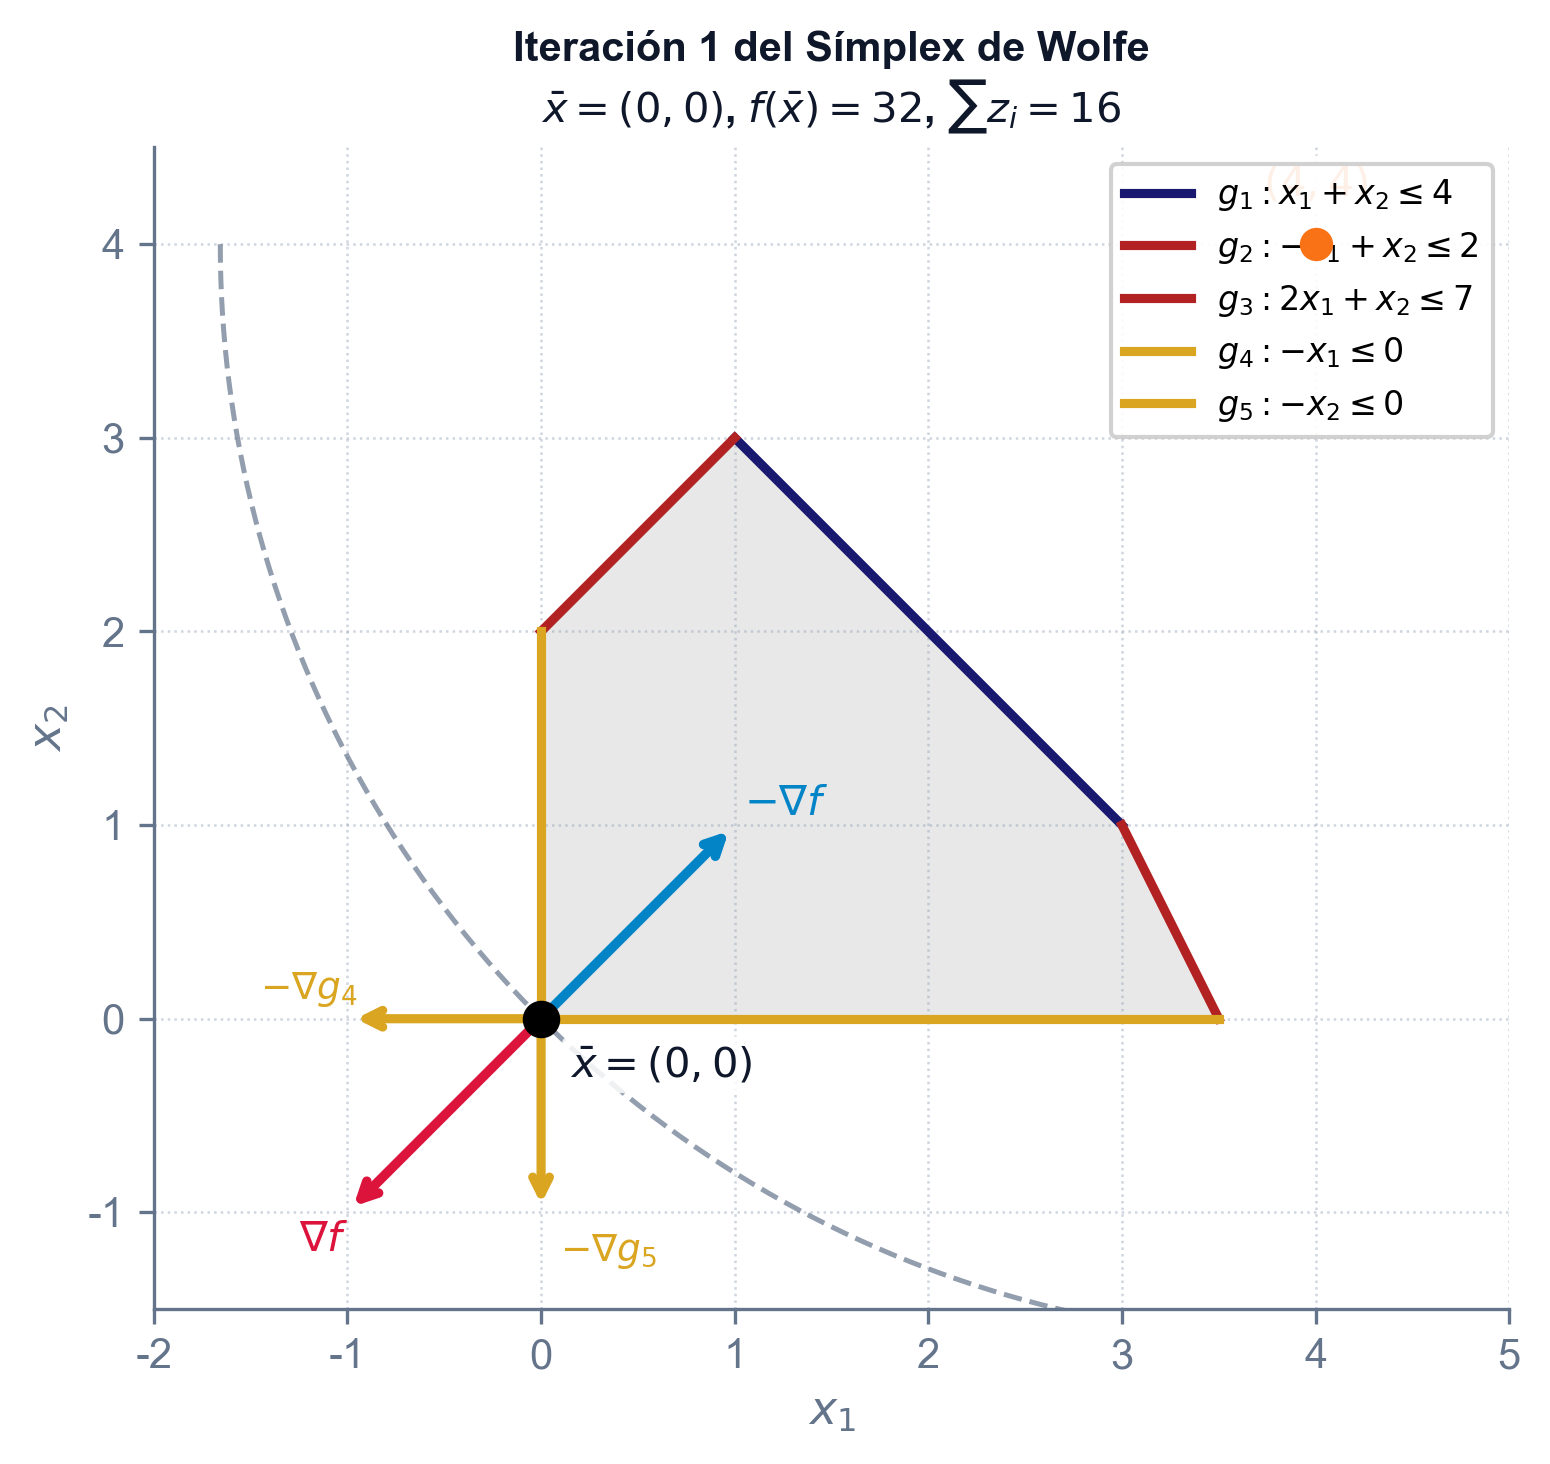
\includegraphics[width=0.7\linewidth,height=\textheight,keepaspectratio]{images/wolfe_iter1.png}

}

\caption{\label{fig-wolfe-iter1}Interpretación geométrica de la
Iteración 1 en el origen (0,0)}

\end{figure}%

\textbf{Iteración 2 (Paso 2: Avance sobre el eje \(X_2\))}\\
En la segunda iteración, la entrada de \(x_2\) en la base desplaza la
solución a lo largo del eje vertical hasta alcanzar el vértice
\(\bar{x} = (0,2)\). En esta posición, la segunda restricción
\(-x_1 + x_2 \le 2\) se vuelve activa (\(y_2 = 0\)), reduciendo el valor
de la función objetivo a \(f(0,2) = 20\) y la suma artificial a
\(\sum z_i = 12\).

\begin{itemize}
\tightlist
\item
  \textbf{Base}: \(\{y_1, x_2, y_3, z_1, z_2\}\), \textbf{Objetivo
  artificial}: \(12\).
\item
  \textbf{Criterio de entrada}: Entra la variable primal
  {\(x_1 \downarrow\)} (coste reducidos \(-4\)). Las variables duales
  \(u_1, u_3\) {continúan bloqueadas} por \(y_1, y_3 \in \text{Base}\).
\item
  \textbf{Pivote}: Abandona la base {\(y_1 \uparrow\)} en la fila 1 con
  pivote \textbf{{2}}.
\end{itemize}

\begin{longtable}[]{@{}
  >{\raggedright\arraybackslash}p{(\linewidth - 26\tabcolsep) * \real{0.0714}}
  >{\raggedright\arraybackslash}p{(\linewidth - 26\tabcolsep) * \real{0.0714}}
  >{\raggedright\arraybackslash}p{(\linewidth - 26\tabcolsep) * \real{0.0714}}
  >{\raggedright\arraybackslash}p{(\linewidth - 26\tabcolsep) * \real{0.0714}}
  >{\raggedright\arraybackslash}p{(\linewidth - 26\tabcolsep) * \real{0.0714}}
  >{\raggedright\arraybackslash}p{(\linewidth - 26\tabcolsep) * \real{0.0714}}
  >{\raggedright\arraybackslash}p{(\linewidth - 26\tabcolsep) * \real{0.0714}}
  >{\raggedright\arraybackslash}p{(\linewidth - 26\tabcolsep) * \real{0.0714}}
  >{\raggedright\arraybackslash}p{(\linewidth - 26\tabcolsep) * \real{0.0714}}
  >{\raggedright\arraybackslash}p{(\linewidth - 26\tabcolsep) * \real{0.0714}}
  >{\raggedright\arraybackslash}p{(\linewidth - 26\tabcolsep) * \real{0.0714}}
  >{\raggedright\arraybackslash}p{(\linewidth - 26\tabcolsep) * \real{0.0714}}
  >{\raggedright\arraybackslash}p{(\linewidth - 26\tabcolsep) * \real{0.0714}}
  >{\raggedright\arraybackslash}p{(\linewidth - 26\tabcolsep) * \real{0.0714}}@{}}
\toprule\noalign{}
\begin{minipage}[b]{\linewidth}\raggedright
Base
\end{minipage} & \begin{minipage}[b]{\linewidth}\raggedright
Sol.
\end{minipage} & \begin{minipage}[b]{\linewidth}\raggedright
\(x_1\)
\end{minipage} & \begin{minipage}[b]{\linewidth}\raggedright
\(x_2\)
\end{minipage} & \begin{minipage}[b]{\linewidth}\raggedright
\(y_1\)
\end{minipage} & \begin{minipage}[b]{\linewidth}\raggedright
\(y_2\)
\end{minipage} & \begin{minipage}[b]{\linewidth}\raggedright
\(y_3\)
\end{minipage} & \begin{minipage}[b]{\linewidth}\raggedright
\(u_1\)
\end{minipage} & \begin{minipage}[b]{\linewidth}\raggedright
\(u_2\)
\end{minipage} & \begin{minipage}[b]{\linewidth}\raggedright
\(u_3\)
\end{minipage} & \begin{minipage}[b]{\linewidth}\raggedright
\(v_1\)
\end{minipage} & \begin{minipage}[b]{\linewidth}\raggedright
\(v_2\)
\end{minipage} & \begin{minipage}[b]{\linewidth}\raggedright
\(z_1\)
\end{minipage} & \begin{minipage}[b]{\linewidth}\raggedright
\(z_2\)
\end{minipage} \\
\midrule\noalign{}
\endhead
\bottomrule\noalign{}
\endlastfoot
\textbf{{\(y_1\)}} & \(2\) & \textbf{{2}} & \(0\) & \(1\) & \(-1\) &
\(0\) & \(0\) & \(0\) & \(0\) & \(0\) & \(0\) & \(0\) & \(0\) \\
\textbf{\(x_2\)} & \(2\) & \(-1\) & \(1\) & \(0\) & \(1\) & \(0\) &
\(0\) & \(0\) & \(0\) & \(0\) & \(0\) & \(0\) & \(0\) \\
\textbf{\(y_3\)} & \(5\) & \(3\) & \(0\) & \(-1\) & \(-1\) & \(1\) &
\(0\) & \(0\) & \(0\) & \(0\) & \(0\) & \(0\) & \(0\) \\
\textbf{\(z_1\)} & \(8\) & \(2\) & \(0\) & \(0\) & \(0\) & \(0\) & \(1\)
& \(-1\) & \(2\) & \(-1\) & \(0\) & \(1\) & \(0\) \\
\textbf{\(z_2\)} & \(4\) & \(2\) & \(0\) & \(0\) & \(-2\) & \(0\) &
\(1\) & \(1\) & \(1\) & \(0\) & \(-1\) & \(0\) & \(1\) \\
\textbf{Coste} & \(12\) & {\(-4\)} & \(0\) & \(0\) & \(2\) & \(0\) &
{\(-2\)} & \(0\) & {\(-3\)} & \(1\) & \(1\) & \(0\) & \(0\) \\
\end{longtable}

Geométricamente, el punto se desplaza sobre el eje \(X_2\) hasta el
vértice \(\bar{x} = (0,2)\), donde se activa la restricción
\(-x_1 + x_2 \le 2\) (\(y_2 = 0\)).

\begin{figure}[H]

\centering{

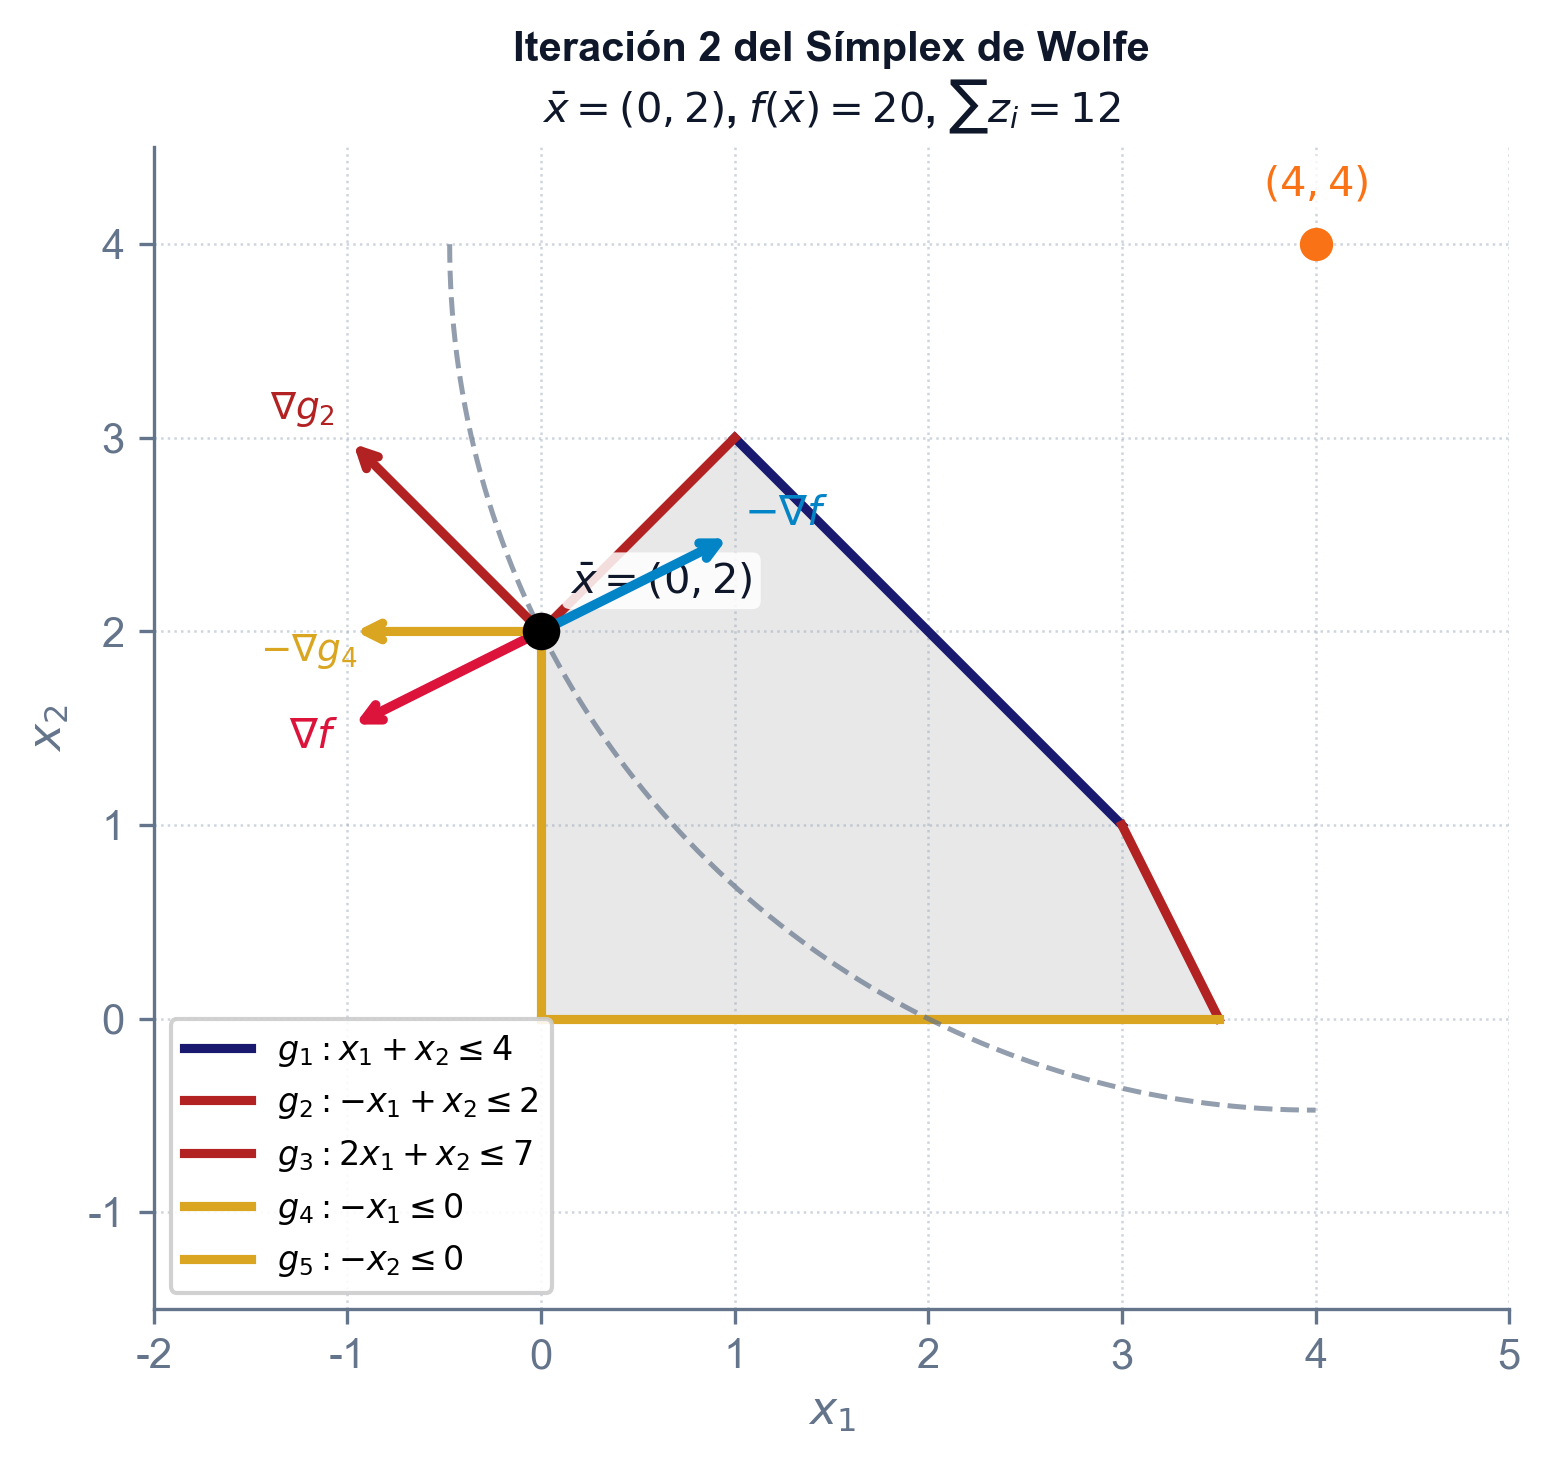
\includegraphics[width=0.7\linewidth,height=\textheight,keepaspectratio]{images/wolfe_iter2.png}

}

\caption{\label{fig-wolfe-iter2}Interpretación geométrica de la
Iteración 2 en el vértice (0,2)}

\end{figure}%

\textbf{Iteración 3 (Paso 3: Desplazamiento al vértice (1,3) y
desbloqueo dual)}\\
En la tercera iteración, al haber salido \(y_1\) de la base en la
iteración anterior, se desactiva el bloqueo de holgura complementaria
sobre la variable dual \(u_1\), permitiendo su entrada. El punto
candidato se desplaza sobre la arista del poliedro \(-x_1 + x_2 = 2\)
hasta situarse en el vértice \(\bar{x} = (1,3)\), activando
simultáneamente la restricción \(x_1 + x_2 \le 4\) (\(y_1 = 0\)), con
\(f(1,3) = 10\) y una suma artificial de \(\sum z_i = 8\).

\begin{itemize}
\tightlist
\item
  \textbf{Base}: \(\{x_1, x_2, y_3, z_1, z_2\}\), \textbf{Objetivo
  artificial}: \(8\).
\item
  \textbf{Criterio de entrada}: Al salir \(y_1\) de la base en la
  iteración anterior, la variable dual {\(u_1 \downarrow\)} {queda libre
  y entra} en la base (coste reducido \(-2\)). La variable \(u_3\) sigue
  bloqueada por \(y_3 \in \text{Base}\).
\item
  \textbf{Pivote}: Abandona la base la variable artificial
  {\(z_2 \uparrow\)} en la fila 5 con elemento pivote \textbf{{1}}.
\end{itemize}

\begin{longtable}[]{@{}
  >{\raggedright\arraybackslash}p{(\linewidth - 26\tabcolsep) * \real{0.0714}}
  >{\raggedright\arraybackslash}p{(\linewidth - 26\tabcolsep) * \real{0.0714}}
  >{\raggedright\arraybackslash}p{(\linewidth - 26\tabcolsep) * \real{0.0714}}
  >{\raggedright\arraybackslash}p{(\linewidth - 26\tabcolsep) * \real{0.0714}}
  >{\raggedright\arraybackslash}p{(\linewidth - 26\tabcolsep) * \real{0.0714}}
  >{\raggedright\arraybackslash}p{(\linewidth - 26\tabcolsep) * \real{0.0714}}
  >{\raggedright\arraybackslash}p{(\linewidth - 26\tabcolsep) * \real{0.0714}}
  >{\raggedright\arraybackslash}p{(\linewidth - 26\tabcolsep) * \real{0.0714}}
  >{\raggedright\arraybackslash}p{(\linewidth - 26\tabcolsep) * \real{0.0714}}
  >{\raggedright\arraybackslash}p{(\linewidth - 26\tabcolsep) * \real{0.0714}}
  >{\raggedright\arraybackslash}p{(\linewidth - 26\tabcolsep) * \real{0.0714}}
  >{\raggedright\arraybackslash}p{(\linewidth - 26\tabcolsep) * \real{0.0714}}
  >{\raggedright\arraybackslash}p{(\linewidth - 26\tabcolsep) * \real{0.0714}}
  >{\raggedright\arraybackslash}p{(\linewidth - 26\tabcolsep) * \real{0.0714}}@{}}
\toprule\noalign{}
\begin{minipage}[b]{\linewidth}\raggedright
Base
\end{minipage} & \begin{minipage}[b]{\linewidth}\raggedright
Sol.
\end{minipage} & \begin{minipage}[b]{\linewidth}\raggedright
\(x_1\)
\end{minipage} & \begin{minipage}[b]{\linewidth}\raggedright
\(x_2\)
\end{minipage} & \begin{minipage}[b]{\linewidth}\raggedright
\(y_1\)
\end{minipage} & \begin{minipage}[b]{\linewidth}\raggedright
\(y_2\)
\end{minipage} & \begin{minipage}[b]{\linewidth}\raggedright
\(y_3\)
\end{minipage} & \begin{minipage}[b]{\linewidth}\raggedright
\(u_1\)
\end{minipage} & \begin{minipage}[b]{\linewidth}\raggedright
\(u_2\)
\end{minipage} & \begin{minipage}[b]{\linewidth}\raggedright
\(u_3\)
\end{minipage} & \begin{minipage}[b]{\linewidth}\raggedright
\(v_1\)
\end{minipage} & \begin{minipage}[b]{\linewidth}\raggedright
\(v_2\)
\end{minipage} & \begin{minipage}[b]{\linewidth}\raggedright
\(z_1\)
\end{minipage} & \begin{minipage}[b]{\linewidth}\raggedright
\(z_2\)
\end{minipage} \\
\midrule\noalign{}
\endhead
\bottomrule\noalign{}
\endlastfoot
\textbf{\(x_1\)} & \(1\) & \(1\) & \(0\) & \(1/2\) & \(-1/2\) & \(0\) &
\(0\) & \(0\) & \(0\) & \(0\) & \(0\) & \(0\) & \(0\) \\
\textbf{\(x_2\)} & \(3\) & \(0\) & \(1\) & \(1/2\) & \(1/2\) & \(0\) &
\(0\) & \(0\) & \(0\) & \(0\) & \(0\) & \(0\) & \(0\) \\
\textbf{\(y_3\)} & \(2\) & \(0\) & \(0\) & \(-5/2\) & \(1/2\) & \(1\) &
\(0\) & \(0\) & \(0\) & \(0\) & \(0\) & \(0\) & \(0\) \\
\textbf{\(z_1\)} & \(6\) & \(0\) & \(0\) & \(-1\) & \(1\) & \(0\) &
\(1\) & \(-1\) & \(2\) & \(-1\) & \(0\) & \(1\) & \(0\) \\
\textbf{{\(z_2\)}} & \(2\) & \(0\) & \(0\) & \(-1\) & \(-1\) & \(0\) &
\textbf{{1}} & \(1\) & \(1\) & \(0\) & \(-1\) & \(0\) & \(1\) \\
\textbf{Coste} & \(8\) & \(0\) & \(0\) & \(2\) & \(0\) & \(0\) &
{\(-2\)} & \(0\) & {\(-3\)} & \(1\) & \(1\) & \(0\) & \(0\) \\
\end{longtable}

Geométricamente, el candidato avanza sobre el borde \(-x_1 + x_2 = 2\)
hasta alcanzar el vértice \(\bar{x} = (1,3)\), donde se activa
adicionalmente \(x_1 + x_2 \le 4\) (\(y_1 = 0\)).

\begin{figure}[H]

\centering{

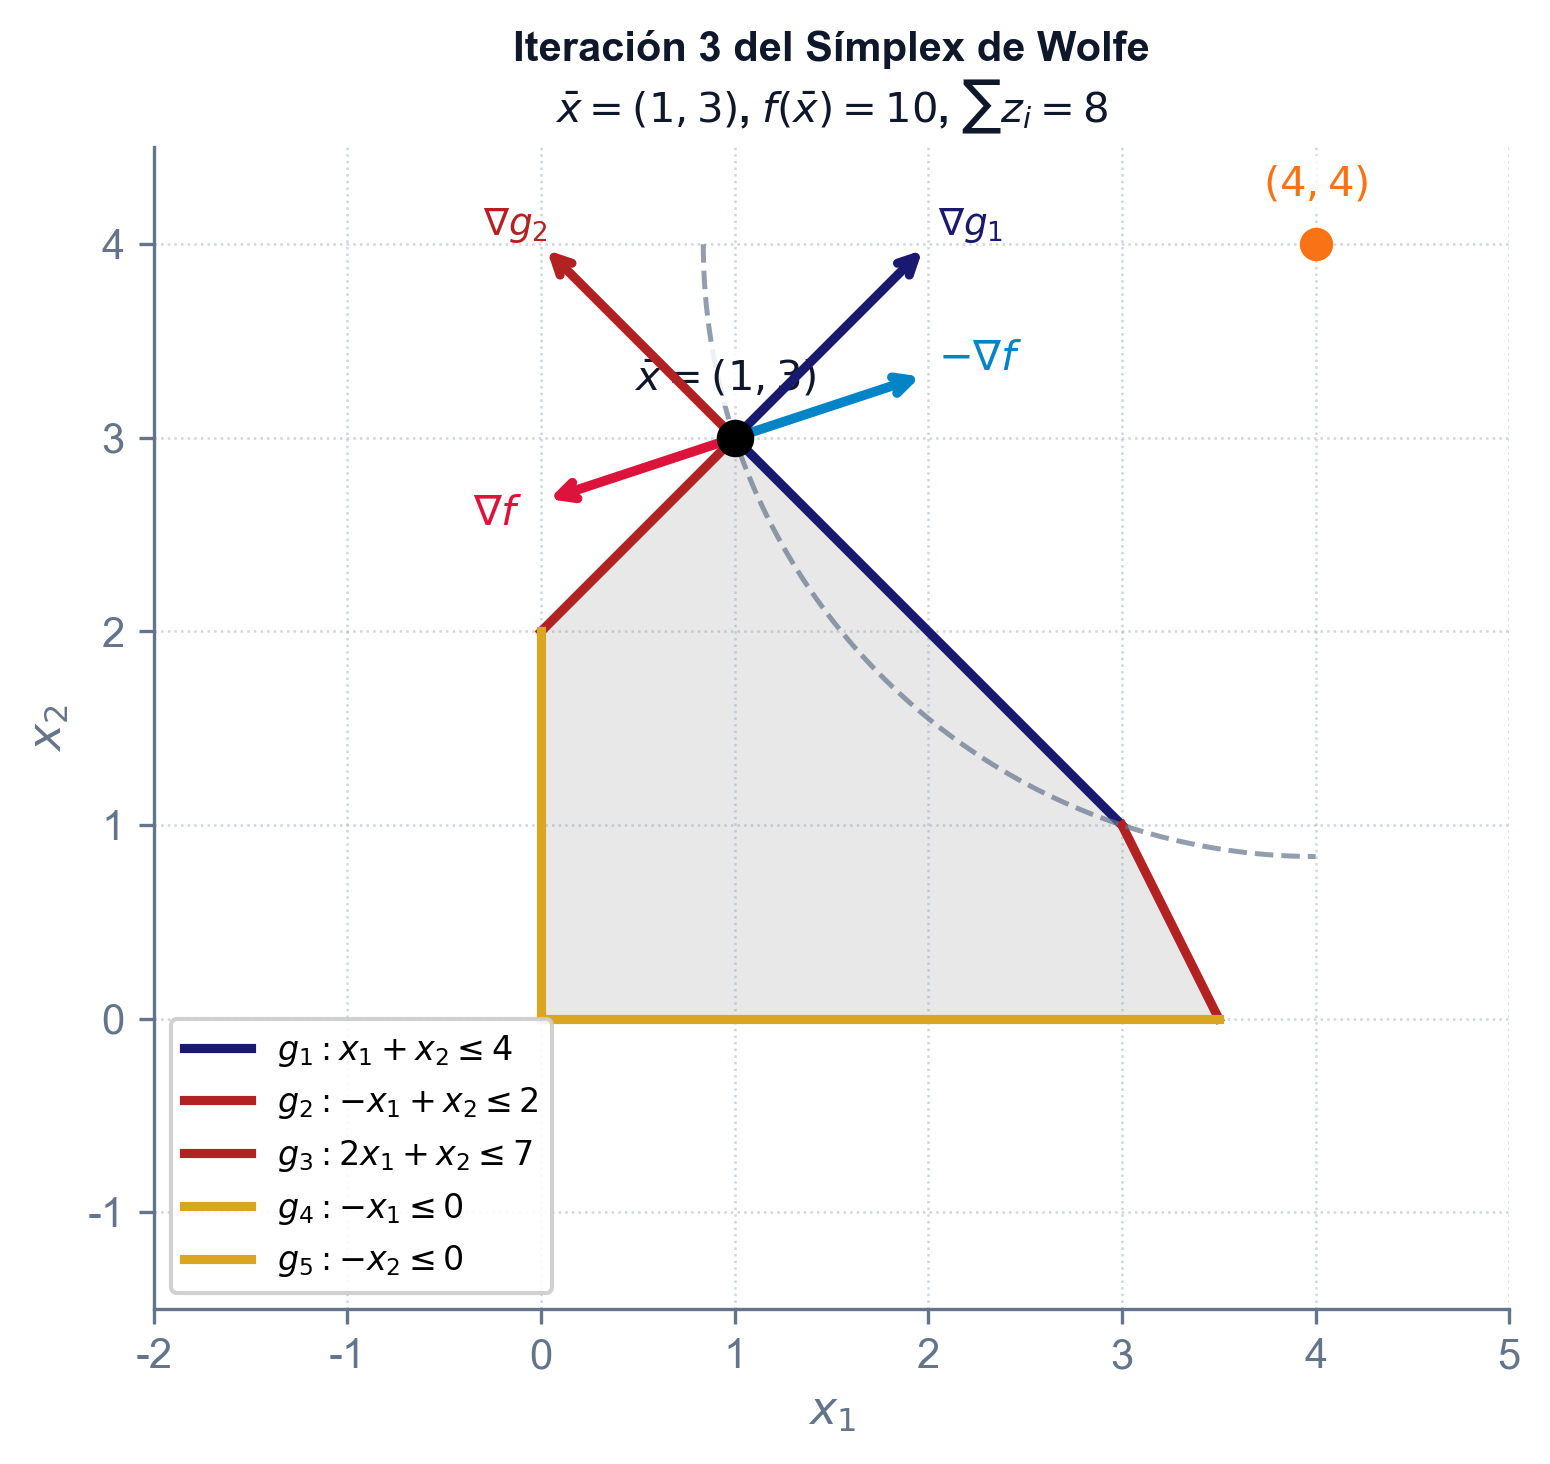
\includegraphics[width=0.7\linewidth,height=\textheight,keepaspectratio]{images/wolfe_iter3.png}

}

\caption{\label{fig-wolfe-iter3}Interpretación geométrica de la
Iteración 3 en el vértice (1,3)}

\end{figure}%

\textbf{Iteración 4 (Paso 4: Ajuste de tensión dual en (1,3))}\\
En la cuarta iteración, la solución primal se mantiene estática en el
vértice \(\bar{x} = (1,3)\), pero se produce un reajuste algebraico en
las variables duales. La variable \(u_1\) entra formalmente en la base
con valor \(u_1 = 2\), eliminando la primera variable artificial \(z_2\)
y reduciendo la función objetivo auxiliar a \(\sum z_i = 4\).

\begin{itemize}
\tightlist
\item
  \textbf{Base}: \(\{x_1, x_2, y_3, z_1, u_1\}\), \textbf{Objetivo
  artificial}: \(4\).
\item
  \textbf{Criterio de entrada}: Entra la variable de holgura
  {\(y_2 \downarrow\)} (coste reducido \(-2\)).
\item
  \textbf{Pivote}: Sale de la base la última variable artificial
  {\(z_1 \uparrow\)} en la fila 4 con pivote \textbf{{2}}.
\end{itemize}

\begin{longtable}[]{@{}
  >{\raggedright\arraybackslash}p{(\linewidth - 26\tabcolsep) * \real{0.0714}}
  >{\raggedright\arraybackslash}p{(\linewidth - 26\tabcolsep) * \real{0.0714}}
  >{\raggedright\arraybackslash}p{(\linewidth - 26\tabcolsep) * \real{0.0714}}
  >{\raggedright\arraybackslash}p{(\linewidth - 26\tabcolsep) * \real{0.0714}}
  >{\raggedright\arraybackslash}p{(\linewidth - 26\tabcolsep) * \real{0.0714}}
  >{\raggedright\arraybackslash}p{(\linewidth - 26\tabcolsep) * \real{0.0714}}
  >{\raggedright\arraybackslash}p{(\linewidth - 26\tabcolsep) * \real{0.0714}}
  >{\raggedright\arraybackslash}p{(\linewidth - 26\tabcolsep) * \real{0.0714}}
  >{\raggedright\arraybackslash}p{(\linewidth - 26\tabcolsep) * \real{0.0714}}
  >{\raggedright\arraybackslash}p{(\linewidth - 26\tabcolsep) * \real{0.0714}}
  >{\raggedright\arraybackslash}p{(\linewidth - 26\tabcolsep) * \real{0.0714}}
  >{\raggedright\arraybackslash}p{(\linewidth - 26\tabcolsep) * \real{0.0714}}
  >{\raggedright\arraybackslash}p{(\linewidth - 26\tabcolsep) * \real{0.0714}}
  >{\raggedright\arraybackslash}p{(\linewidth - 26\tabcolsep) * \real{0.0714}}@{}}
\toprule\noalign{}
\begin{minipage}[b]{\linewidth}\raggedright
Base
\end{minipage} & \begin{minipage}[b]{\linewidth}\raggedright
Sol.
\end{minipage} & \begin{minipage}[b]{\linewidth}\raggedright
\(x_1\)
\end{minipage} & \begin{minipage}[b]{\linewidth}\raggedright
\(x_2\)
\end{minipage} & \begin{minipage}[b]{\linewidth}\raggedright
\(y_1\)
\end{minipage} & \begin{minipage}[b]{\linewidth}\raggedright
\(y_2\)
\end{minipage} & \begin{minipage}[b]{\linewidth}\raggedright
\(y_3\)
\end{minipage} & \begin{minipage}[b]{\linewidth}\raggedright
\(u_1\)
\end{minipage} & \begin{minipage}[b]{\linewidth}\raggedright
\(u_2\)
\end{minipage} & \begin{minipage}[b]{\linewidth}\raggedright
\(u_3\)
\end{minipage} & \begin{minipage}[b]{\linewidth}\raggedright
\(v_1\)
\end{minipage} & \begin{minipage}[b]{\linewidth}\raggedright
\(v_2\)
\end{minipage} & \begin{minipage}[b]{\linewidth}\raggedright
\(z_1\)
\end{minipage} & \begin{minipage}[b]{\linewidth}\raggedright
\(z_2\)
\end{minipage} \\
\midrule\noalign{}
\endhead
\bottomrule\noalign{}
\endlastfoot
\textbf{\(x_1\)} & \(1\) & \(1\) & \(0\) & \(1/2\) & \(-1/2\) & \(0\) &
\(0\) & \(0\) & \(0\) & \(0\) & \(0\) & \(0\) & \(0\) \\
\textbf{\(x_2\)} & \(3\) & \(0\) & \(1\) & \(1/2\) & \(1/2\) & \(0\) &
\(0\) & \(0\) & \(0\) & \(0\) & \(0\) & \(0\) & \(0\) \\
\textbf{\(y_3\)} & \(2\) & \(0\) & \(0\) & \(-5/2\) & \(1/2\) & \(1\) &
\(0\) & \(0\) & \(0\) & \(0\) & \(0\) & \(0\) & \(0\) \\
\textbf{{\(z_1\)}} & \(4\) & \(0\) & \(0\) & \(0\) & \textbf{{2}} &
\(0\) & \(0\) & \(-2\) & \(1\) & \(-1\) & \(-1\) & \(1\) & \(-1\) \\
\textbf{\(u_1\)} & \(2\) & \(0\) & \(0\) & \(-1\) & \(-1\) & \(0\) &
\(1\) & \(1\) & \(1\) & \(0\) & \(-1\) & \(0\) & \(1\) \\
\textbf{Coste} & \(4\) & \(0\) & \(0\) & \(0\) & {\(-2\)} & \(0\) &
\(0\) & \(2\) & {\(-1\)} & \(1\) & {\(-1\)} & \(0\) & \(2\) \\
\end{longtable}

Geométricamente, el punto en el espacio primal permanece en el vértice
\(\bar{x} = (1,3)\) mientras se ajusta la tensión del multiplicador dual
(\(u_1 = 2\)).

\begin{figure}[H]

\centering{

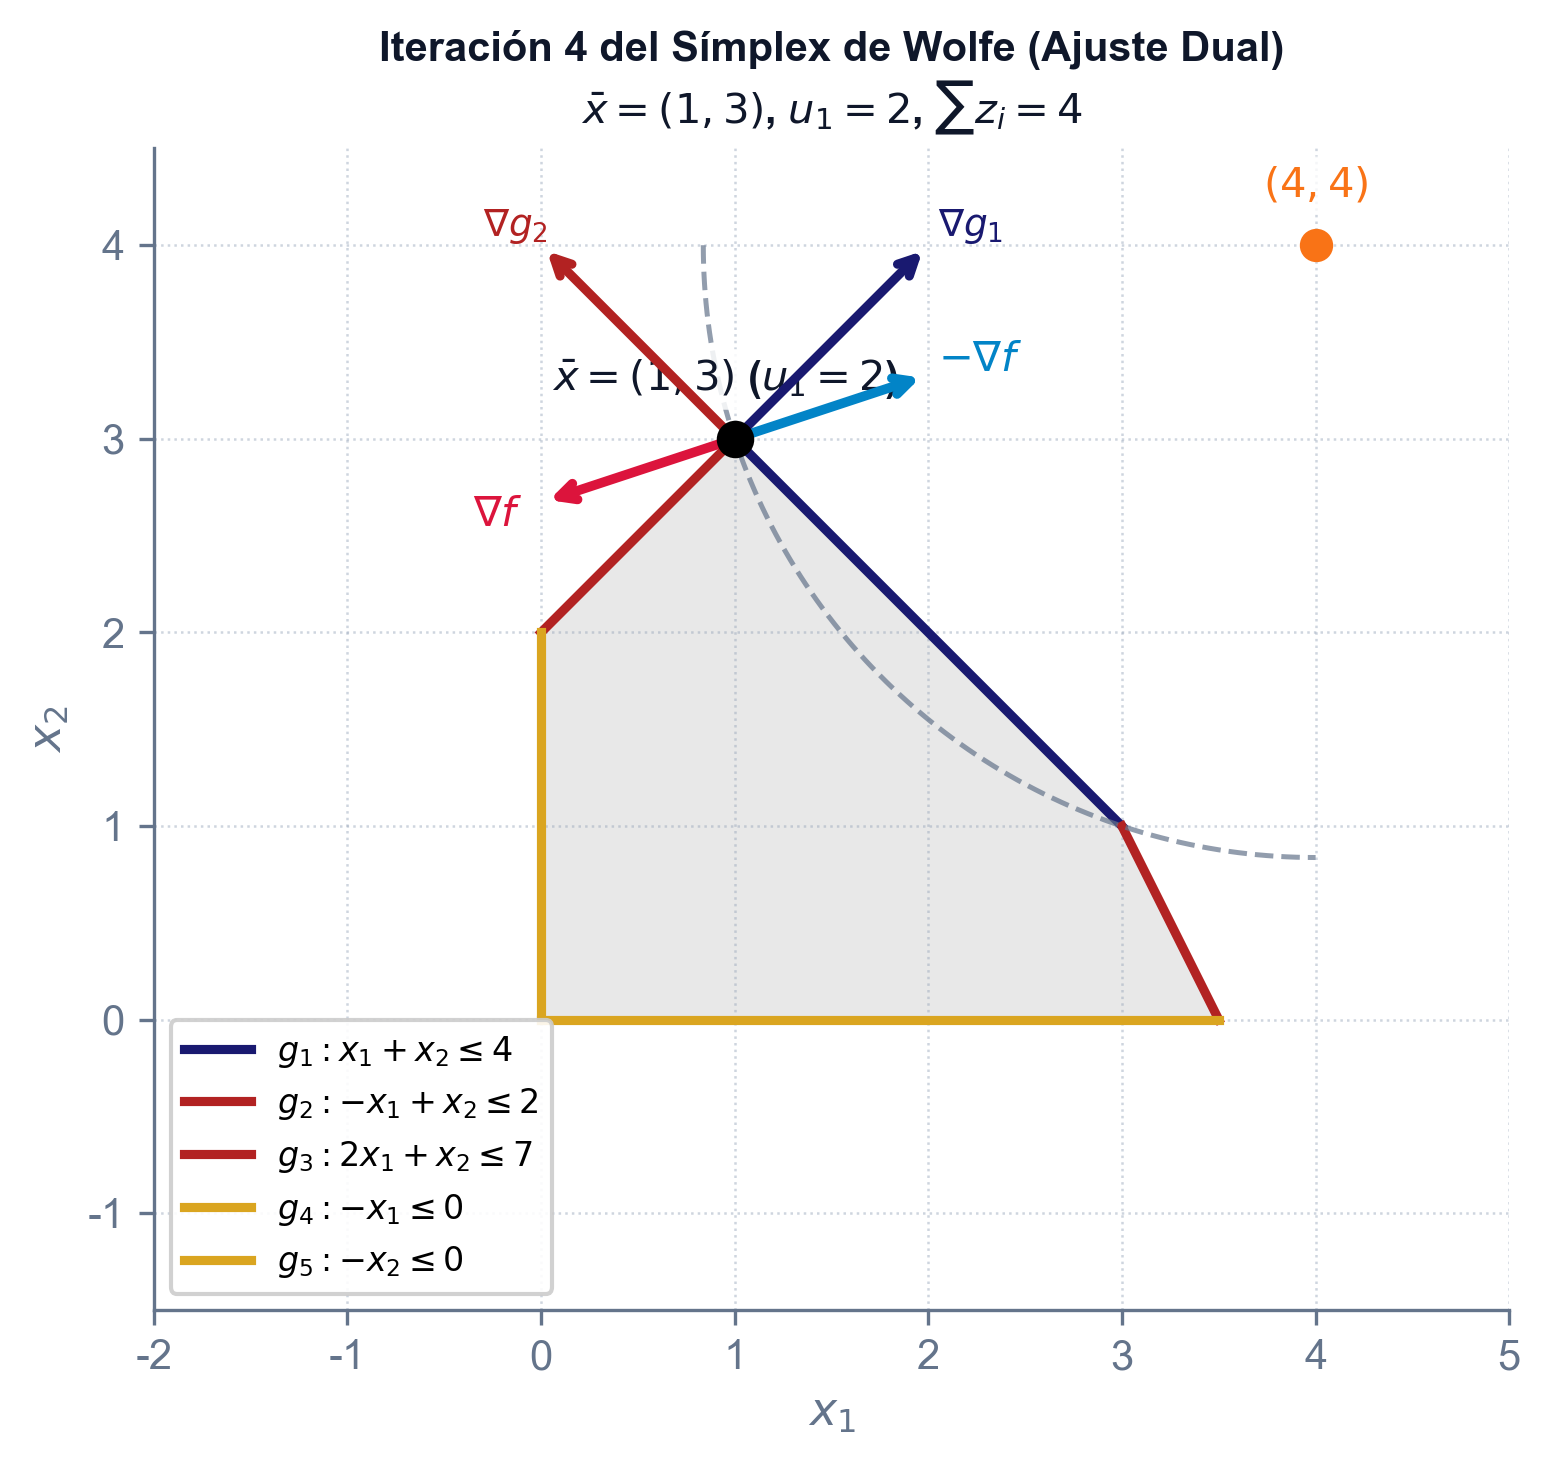
\includegraphics[width=0.7\linewidth,height=\textheight,keepaspectratio]{images/wolfe_iter4.png}

}

\caption{\label{fig-wolfe-iter4}Interpretación geométrica de la
Iteración 4 (Ajuste Dual en (1,3))}

\end{figure}%

\textbf{Iteración 5 (Paso 5: Consecución del Óptimo Global y Tangencia
en (2,2))}\\
En la quinta iteración, la entrada de la holgura \(y_2\) permite que el
punto abandone el vértice \((1,3)\) y se deslice a lo largo del segmento
de la restricción activa \(x_1 + x_2 = 4\) hasta el punto
\(\bar{x} = (2,2)\). En este punto se alcanza la tangencia con la
superficie cuadrática de nivel de la función objetivo, anulando por
completo las variables artificiales (\(\sum z_i = 0\)), fijando el
multiplicador dual activo \(u_1^* = 4\) y alcanzando el coste mínimo de
\(f(2,2) = 8\).

\begin{itemize}
\tightlist
\item
  \textbf{Base óptima}: \(\{x_1, x_2, y_3, y_2, u_1\}\),
  \textbf{Objetivo artificial}: \(0\).
\item
  \textbf{Criterio de parada}: Todas las variables artificiales han
  salido de la base (\(z_1^* = 0, z_2^* = 0\)) y no existen costes
  reducidos negativos viables bajo la regla de entrada restringida.
\end{itemize}

\begin{longtable}[]{@{}
  >{\raggedright\arraybackslash}p{(\linewidth - 26\tabcolsep) * \real{0.0714}}
  >{\raggedright\arraybackslash}p{(\linewidth - 26\tabcolsep) * \real{0.0714}}
  >{\raggedright\arraybackslash}p{(\linewidth - 26\tabcolsep) * \real{0.0714}}
  >{\raggedright\arraybackslash}p{(\linewidth - 26\tabcolsep) * \real{0.0714}}
  >{\raggedright\arraybackslash}p{(\linewidth - 26\tabcolsep) * \real{0.0714}}
  >{\raggedright\arraybackslash}p{(\linewidth - 26\tabcolsep) * \real{0.0714}}
  >{\raggedright\arraybackslash}p{(\linewidth - 26\tabcolsep) * \real{0.0714}}
  >{\raggedright\arraybackslash}p{(\linewidth - 26\tabcolsep) * \real{0.0714}}
  >{\raggedright\arraybackslash}p{(\linewidth - 26\tabcolsep) * \real{0.0714}}
  >{\raggedright\arraybackslash}p{(\linewidth - 26\tabcolsep) * \real{0.0714}}
  >{\raggedright\arraybackslash}p{(\linewidth - 26\tabcolsep) * \real{0.0714}}
  >{\raggedright\arraybackslash}p{(\linewidth - 26\tabcolsep) * \real{0.0714}}
  >{\raggedright\arraybackslash}p{(\linewidth - 26\tabcolsep) * \real{0.0714}}
  >{\raggedright\arraybackslash}p{(\linewidth - 26\tabcolsep) * \real{0.0714}}@{}}
\toprule\noalign{}
\begin{minipage}[b]{\linewidth}\raggedright
Base
\end{minipage} & \begin{minipage}[b]{\linewidth}\raggedright
Sol.
\end{minipage} & \begin{minipage}[b]{\linewidth}\raggedright
\(x_1\)
\end{minipage} & \begin{minipage}[b]{\linewidth}\raggedright
\(x_2\)
\end{minipage} & \begin{minipage}[b]{\linewidth}\raggedright
\(y_1\)
\end{minipage} & \begin{minipage}[b]{\linewidth}\raggedright
\(y_2\)
\end{minipage} & \begin{minipage}[b]{\linewidth}\raggedright
\(y_3\)
\end{minipage} & \begin{minipage}[b]{\linewidth}\raggedright
\(u_1\)
\end{minipage} & \begin{minipage}[b]{\linewidth}\raggedright
\(u_2\)
\end{minipage} & \begin{minipage}[b]{\linewidth}\raggedright
\(u_3\)
\end{minipage} & \begin{minipage}[b]{\linewidth}\raggedright
\(v_1\)
\end{minipage} & \begin{minipage}[b]{\linewidth}\raggedright
\(v_2\)
\end{minipage} & \begin{minipage}[b]{\linewidth}\raggedright
\(z_1\)
\end{minipage} & \begin{minipage}[b]{\linewidth}\raggedright
\(z_2\)
\end{minipage} \\
\midrule\noalign{}
\endhead
\bottomrule\noalign{}
\endlastfoot
\textbf{\(x_1\)} & \(2\) & \(1\) & \(0\) & \(1/2\) & \(0\) & \(0\) &
\(0\) & \(-1/2\) & \(1/4\) & \(-1/4\) & \(1/4\) & \(1/4\) & \(-1/4\) \\
\textbf{\(x_2\)} & \(2\) & \(0\) & \(1\) & \(1/2\) & \(0\) & \(0\) &
\(0\) & \(1/2\) & \(-1/4\) & \(1/4\) & \(-1/4\) & \(-1/4\) & \(1/4\) \\
\textbf{\(y_3\)} & \(1\) & \(0\) & \(0\) & \(-5/2\) & \(0\) & \(1\) &
\(0\) & \(1/2\) & \(-1/4\) & \(1/4\) & \(-1/4\) & \(-1/4\) & \(1/4\) \\
\textbf{\(y_2\)} & \(2\) & \(0\) & \(0\) & \(0\) & \(1\) & \(0\) & \(0\)
& \(-1\) & \(1/2\) & \(-1/2\) & \(1/2\) & \(1/2\) & \(-1/2\) \\
\textbf{\(u_1\)} & \(4\) & \(0\) & \(0\) & \(-1\) & \(0\) & \(0\) &
\(1\) & \(0\) & \(3/2\) & \(-1/2\) & \(-1/2\) & \(1/2\) & \(1/2\) \\
\textbf{Coste} & \(0\) & \(0\) & \(0\) & \(0\) & \(0\) & \(0\) & \(0\) &
\(0\) & \(0\) & \(0\) & \(0\) & \(1\) & \(1\) \\
\end{longtable}

\textbf{Resultado final}: El punto se desliza sobre la restricción
activa \(x_1 + x_2 = 4\) (\(y_1=0\)) hasta alcanzar el punto óptimo
global \(\bar{x} = (2,2)\) con \(u_1^* = 4\) y valor mínimo de la
función objetivo \(f(2,2) = 8\).

\begin{figure}[H]

\centering{

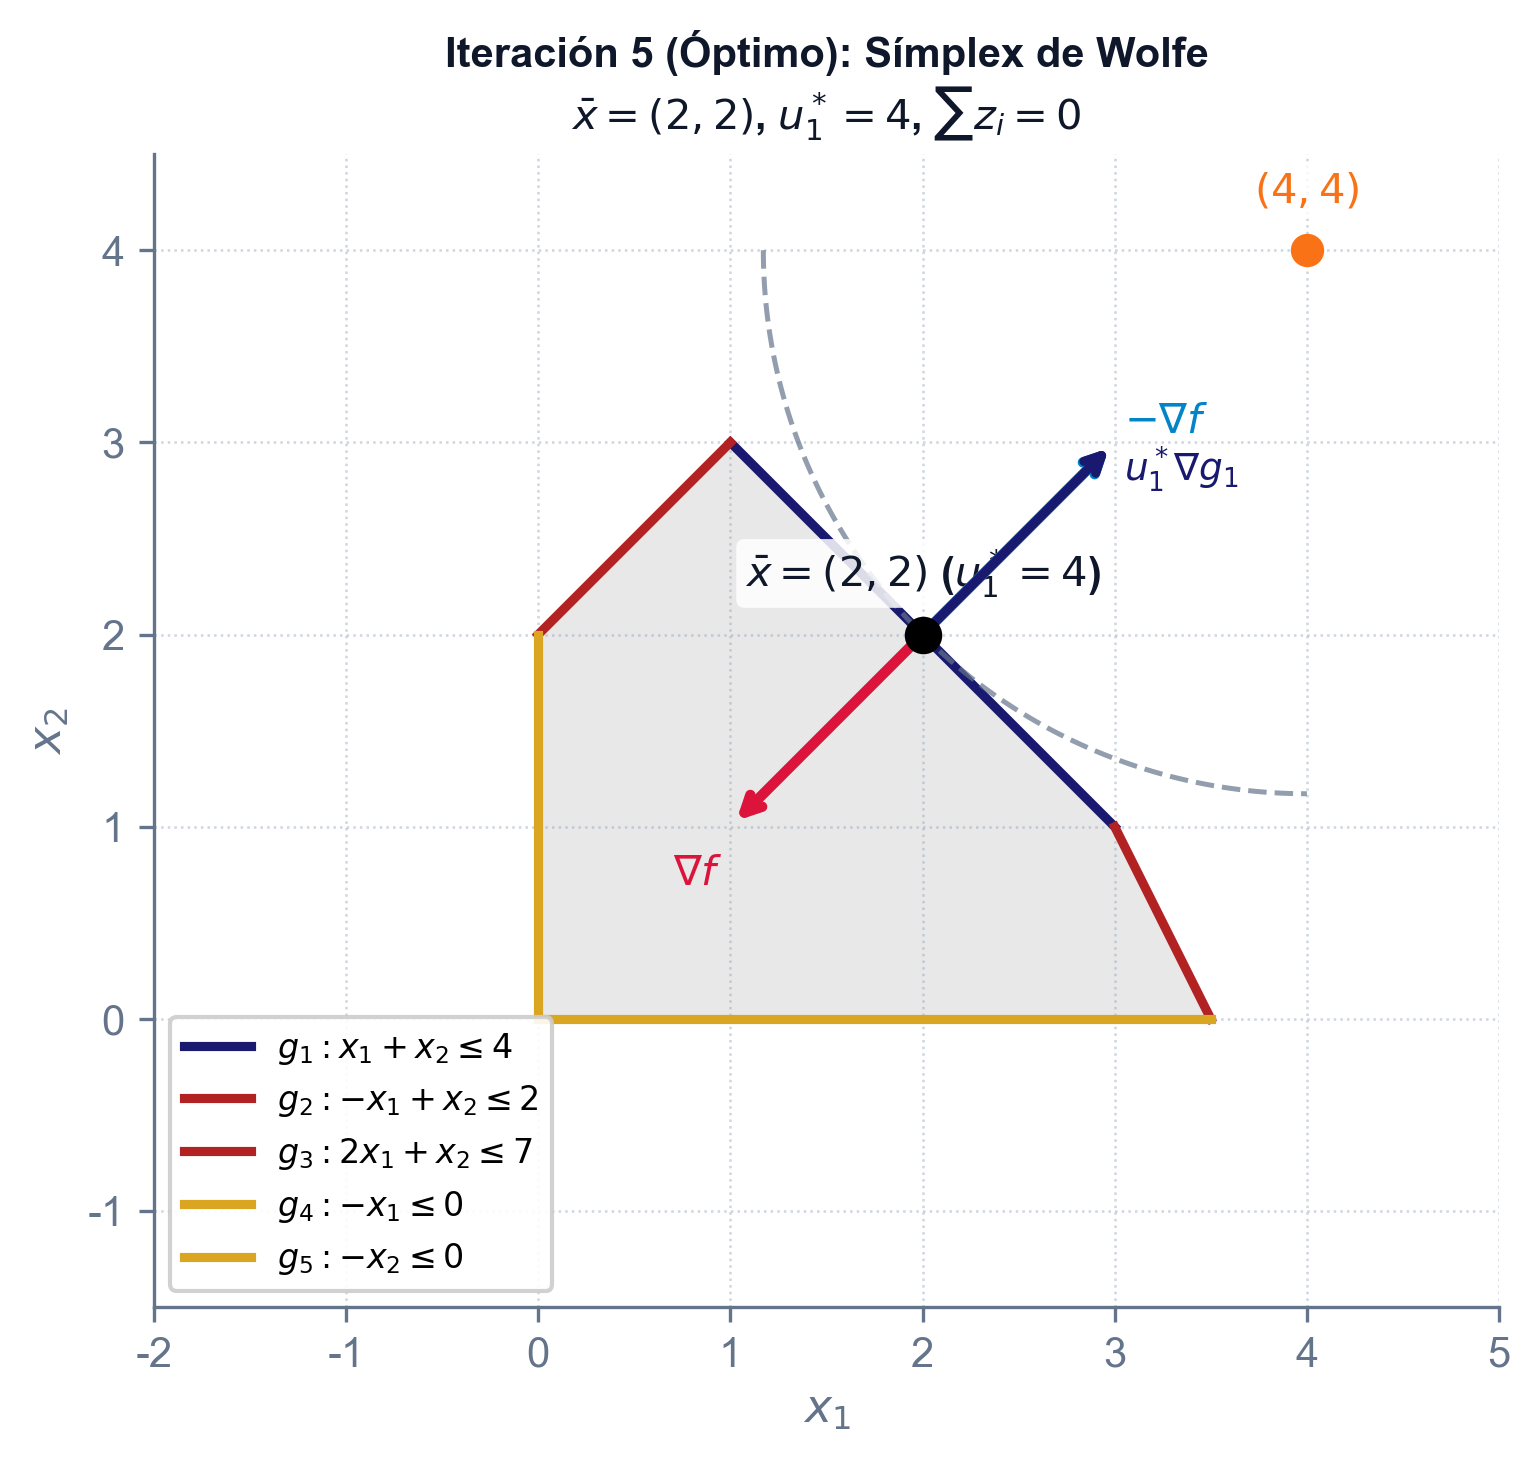
\includegraphics[width=0.7\linewidth,height=\textheight,keepaspectratio]{images/wolfe_iter5.png}

}

\caption{\label{fig-wolfe-iter5}Interpretación geométrica de la
Iteración 5 Óptima en (2,2)}

\end{figure}%

\textbf{Análisis Geométrico de la Trayectoria Completa del Símplex de
Wolfe}\\
La secuencia de pivotes del algoritmo del Símplex de Wolfe dibuja una
trayectoria geométrica precisa sobre el plano \(\mathbb{R}^2\):

\begin{enumerate}
\def\labelenumi{\arabic{enumi}.}
\tightlist
\item
  \textbf{Iteración 1}: Arranca en el origen \((0,0)\).
\item
  \textbf{Iteración 2}: La variable \(x_2\) entra en la base,
  desplazando el punto sobre el eje \(Y\) hasta el vértice \((0,2)\),
  donde se activa la restricción \(-x_1 + x_2 \le 2\) (\(y_2 = 0\)).
\item
  \textbf{Iteración 3}: La variable \(x_1\) entra en la base, avanzando
  por el borde de la restricción \(-x_1 + x_2 = 2\) hasta el vértice
  \((1,3)\), donde se activa además \(x_1 + x_2 \le 4\) (\(y_1 = 0\)).
\item
  \textbf{Iteración 4}: Al anularse \(y_1\), se desbloquea la entrada
  del multiplicador dual \(u_1\). El punto geométrico permanece en
  \((1,3)\) mientras se ajusta la tensión dual (\(u_1 = 2\)).
\item
  \textbf{Iteración 5}: Entra la holgura \(y_2\) (desactivando la
  restricción \(-x_1 + x_2 \le 2\)). El punto se desliza sobre el
  segmento activo \(x_1 + x_2 = 4\) hasta alcanzar el punto más próximo
  al objetivo \((4,4)\), situándose en \((2,2)\) con \(u_1^* = 4\).
\end{enumerate}

La trayectoria geométrica global completa sobre el politopo factible se
ilustra en la Figura~\ref{fig-wolfe-trayectoria}.

\begin{figure}[H]

\centering{

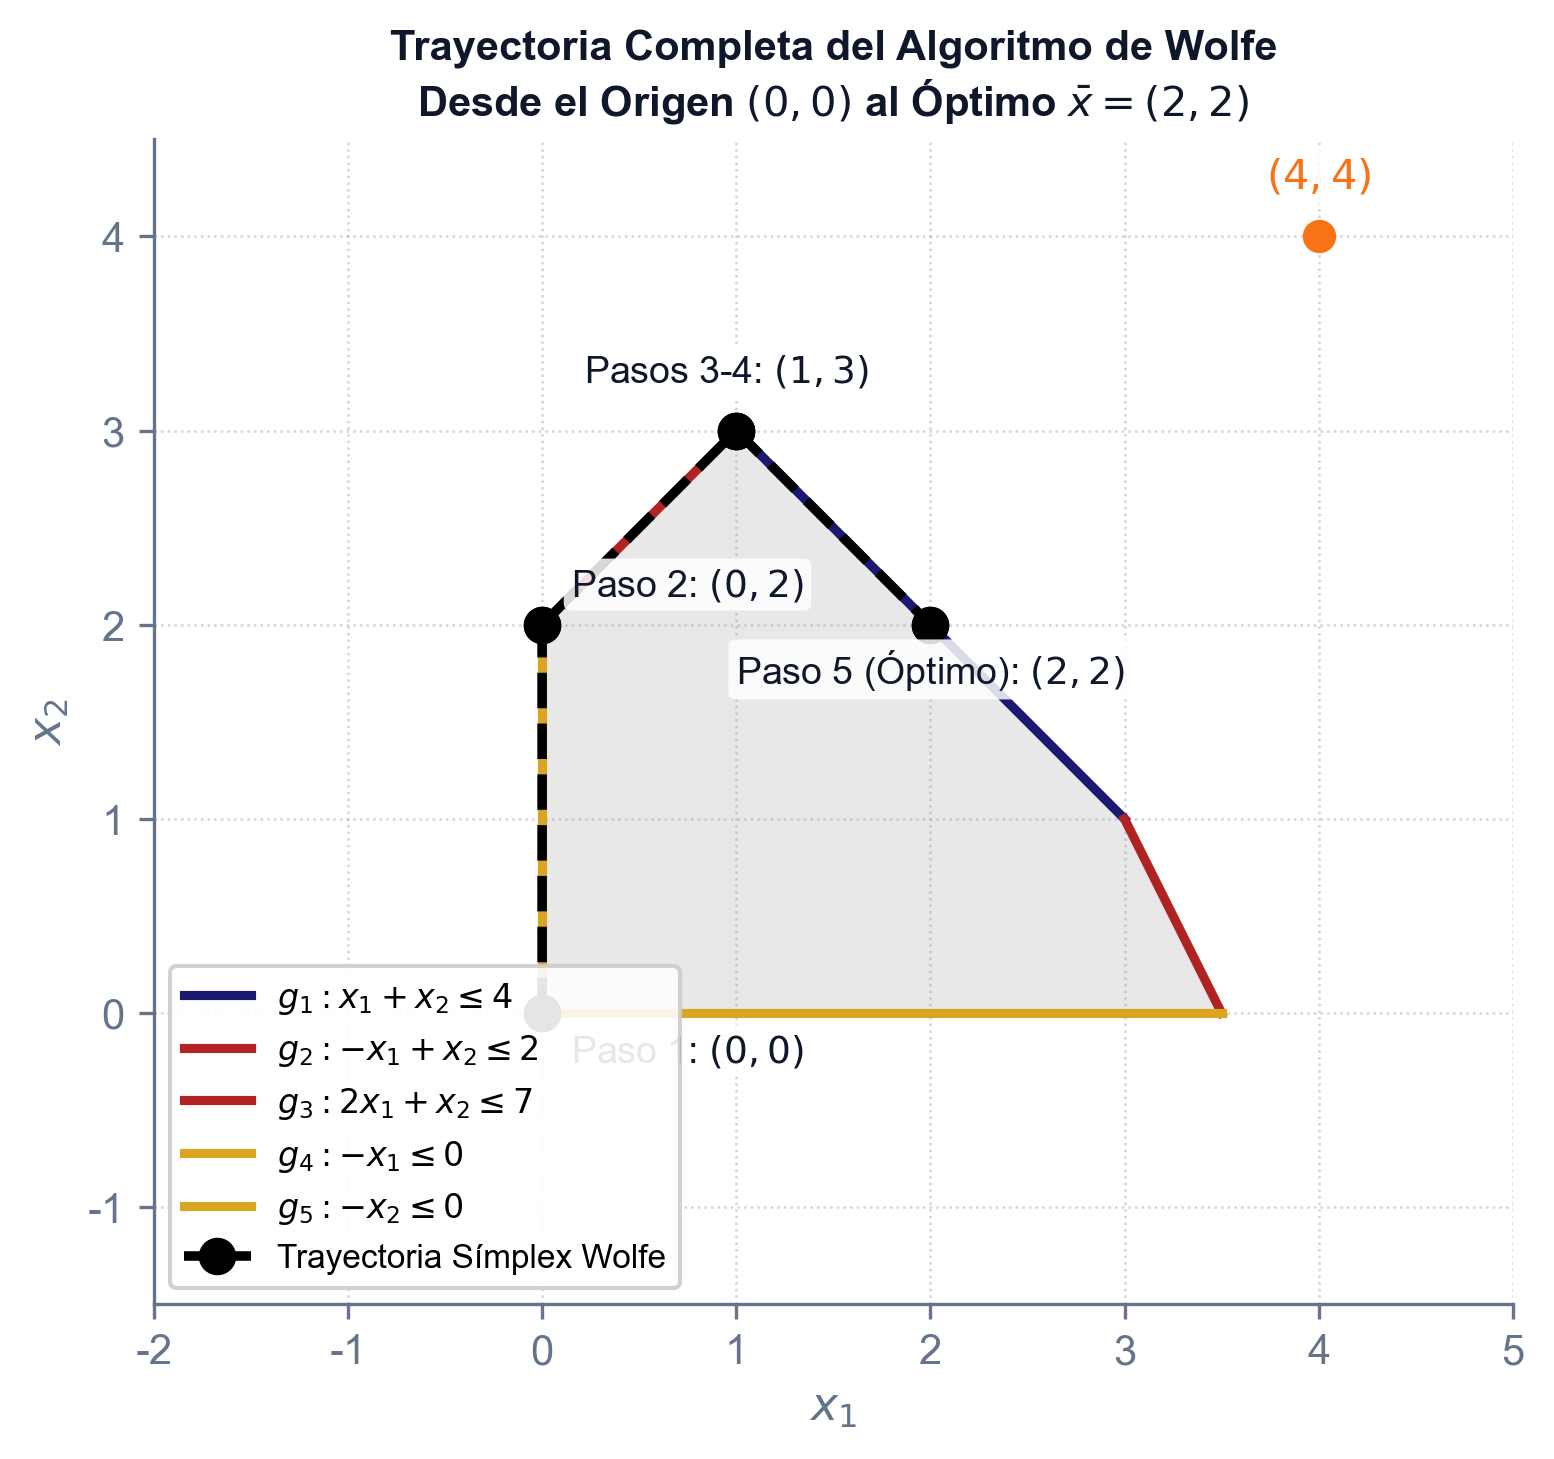
\includegraphics[width=0.75\linewidth,height=\textheight,keepaspectratio]{images/wolfe_trayectoria.png}

}

\caption{\label{fig-wolfe-trayectoria}Trayectoria del algoritmo del
Símplex de Wolfe sobre el politopo factible}

\end{figure}%

\end{tcolorbox}

\section{Consideraciones finales}\label{consideraciones-finales}

En este tema se ha analizado en profundidad la interconexión matemática
existente entre las condiciones de Karush-Kuhn-Tucker (KKT), la teoría
de la dualidad en programación lineal y la resolución computacional de
problemas de programación cuadrática (QP). Los pilares teóricos y
metodológicos fundamentales derivados de este estudio se estructuran a
continuación:

\begin{enumerate}
\def\labelenumi{\arabic{enumi}.}
\item
  \textbf{Equivalencia entre multiplicadores KKT y variables duales}: La
  caracterización de optimalidad KKT para problemas de optimización
  lineal demuestra formalmente que los multiplicadores de Lagrange
  \(u_i^*\) asociados a las restricciones de desigualdad no son meros
  constructos algebraicos, sino que equivalen exactamente a las
  variables óptimas del problema dual. Esta correspondencia biunívoca
  vincula directamente la geometría del politopo primal con el espacio
  de soluciones del dual.
\item
  \textbf{Interpretación económica y precios sombra}: Los
  multiplicadores KKT \(u_i^*\) representan los precios sombra o costes
  marginales de oportunidad asociados a las restricciones del sistema.
  Formalmente, \(u_i^*\) cuantifica la tasa de variación marginal en el
  beneficio o coste óptimo ante un incremento unitario en la término
  independiente \(b_i\). Las condiciones de holgura complementaria
  (\(u_i^* g_i(x^*) = 0\)) aseguran que solo aquellos restricciones
  activas (restricciones activas con \(g_i(x^*)=0\)) presentan un valor
  marginal positivo (\(u_i^* > 0\)), mientras que los restricciones
  inactivas (\(g_i(x^*) < 0\)) poseen un precio sombra nulo
  (\(u_i^* = 0\)).
\item
  \textbf{Estructura matricial y convexidad en programación cuadrática}:
  Al incorporar términos cuadráticos en la función objetivo mediante una
  matriz simétrica semidefinida positiva \(Q \succeq 0\), el problema
  mantiene la convexidad, lo que garantiza que cualquier punto que
  satisfaga las condiciones KKT sea un óptimo global absoluto. Las
  condiciones KKT de un problema QP adoptan la forma de un sistema de
  ecuaciones lineales sobre las variables primales \(x\), de holgura
  \(y\), duales \(u\) y de gradiente \(v\), sujeto únicamente a la
  restricción bilineal de complementariedad.
\item
  \textbf{Fundamento algorítmico del Símplex de Wolfe}: El algoritmo del
  Símplex de Wolfe adapta el mecanismo de pivotaje de la programación
  lineal para resolver el sistema KKT de un problema QP convexo
  imponiendo una regla de entrada restringida. Esta regla prohíbe
  explícitamente que una variable dual \(u_i\) (o \(v_j\)) entre en la
  base si su variable primal complementaria \(y_i\) (o \(x_j\))
  pertenece actualmente a la misma, garantizando el cumplimiento
  estricto de la holgura complementaria en cada iteración del algoritmo.
\item
  \textbf{Dinámica geométrica primal-dual}: A diferencia del Símplex
  lineal clásico ---que se desplaza de vértice en vértice sobre las
  esquinas del politopo---, el Símplex de Wolfe recorre la frontera y
  las caras del conjunto factible \(S\). A lo largo de esta trayectoria,
  el algoritmo combina desplazamientos en el dominio de las variables
  primales con ajustes de tensión en el espacio dual hasta situar la
  solución en el punto exacto de tangencia entre las superficies
  cuadráticas de nivel y el borde activo de las restricciones.
\end{enumerate}

\part{Bloque II: Optimización en redes}

\chapter{Grafos y árboles soporte}\label{grafos-y-uxe1rboles-soporte}

El análisis y la optimización en redes constituye una de las disciplinas
más fértiles y de mayor aplicación práctica en la investigación
operativa, la ingeniería de sistemas, la logística y la ciencia de datos
moderna. El lenguaje formal de la \textbf{teoría de grafos} permite
abstraer la estructura matemática subyacente de sistemas complejos
caracterizados por un conjunto de entidades interconectadas. Desde la
planificación de rutas de transporte aéreo, la gestión del flujo de
carga en redes eléctricas o la distribución de datos en internet, hasta
el agrupamiento no supervisado (\emph{clustering}) en aprendizaje
automático, los grafos proporcionan un marco analítico unificado para
modelar, optimizar y extraer conocimiento sobre la conectividad y la
topología de la información.

\begin{tcolorbox}[enhanced jigsaw, toprule=.15mm, opacitybacktitle=0.6, coltitle=black, colbacktitle=quarto-callout-important-color!10!white, title=\textcolor{quarto-callout-important-color}{\faExclamation}\hspace{0.5em}{Objetivos de aprendizaje}, arc=.35mm, rightrule=.15mm, toptitle=1mm, breakable, bottomtitle=1mm, titlerule=0mm, colback=white, opacityback=0, leftrule=.75mm, colframe=quarto-callout-important-color-frame, left=2mm, bottomrule=.15mm]

Al finalizar este capítulo, serás capaz de:

\begin{enumerate}
\def\labelenumi{\arabic{enumi}.}
\tightlist
\item
  \textbf{Definir} formalmente grafos dirigidos y no dirigidos,
  especificando vecindades, grados de nodos e incidencias de corte.
\item
  \textbf{Diferenciar} rigurosamente entre cadenas, caminos, ciclos y
  circuitos, así como clasificar la conectividad en redes no dirigidas y
  la conexidad fuerte/débil en digrafos.
\item
  \textbf{Demostrar} la Fórmula Planar de Euler y caracterizar la
  topología de grafos planares y bipartitos mediante las construcciones
  de Dudeney y Kuratowski.
\item
  \textbf{Formular} la representación en memoria mediante matrices de
  incidencia con la propiedad de Total Unimodularidad (TUM), matrices de
  adyacencia y la estructura compacta de estrella saliente
  (\emph{Forward Star}).
\item
  \textbf{Caracterizar} las seis propiedades matemáticas equivalentes
  que definen la estructura abstracta de los árboles y bosques.
\item
  \textbf{Aplicar} y comparar los algoritmos de Kruskal y Prim para la
  resolución del problema del Árbol Soporte de Mínimo Peso (MST), y
  \textbf{construir} modelos de agrupamiento jerárquico no supervisado
  (\emph{Single-Linkage Clustering}) en Python.
\end{enumerate}

\end{tcolorbox}

\section{El problema de los puentes de Königsberg (Euler,
1736)}\label{el-problema-de-los-puentes-de-kuxf6nigsberg-euler-1736}

La teoría de grafos nació históricamente en 1736 con la célebre
resolución del \textbf{Problema de los Puentes de Königsberg} formulado
y resuelto por el matemático suizo Leonhard Euler (Euler 1736). La
antigua ciudad de Königsberg (actual Kaliningrado) estaba dividida por
el río Pregel en cuatro masas de tierra diferenciadas: la Isla Kneiphof
(\(A\)), dos orillas principales (\(B\) y \(C\)) y la región oriental de
la bifurcación (\(D\)). Estas cuatro regiones estaban interconectadas
mediante siete puentes de madera, como se ilustra históricamente en las
figuras Figura~\ref{fig-koenigsberg-a}, Figura~\ref{fig-koenigsberg-aa}
y Figura~\ref{fig-koenigsberg-aaa}.

\begin{figure}

\centering{

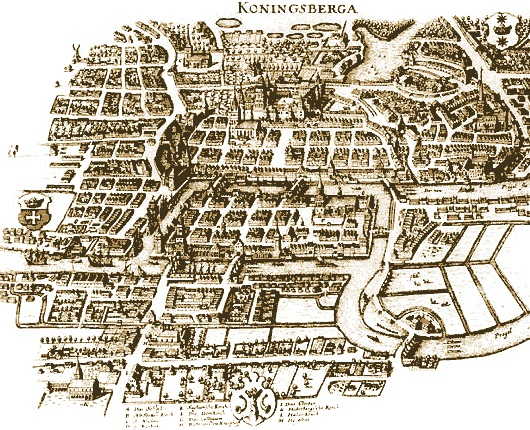
\includegraphics[width=0.7\linewidth,height=\textheight,keepaspectratio]{images/fig_koenigsberg_a.jpg}

}

\caption{\label{fig-koenigsberg-a}Grabado histórico original de la
ciudad de Königsberg}

\end{figure}%

\begin{figure}

\centering{

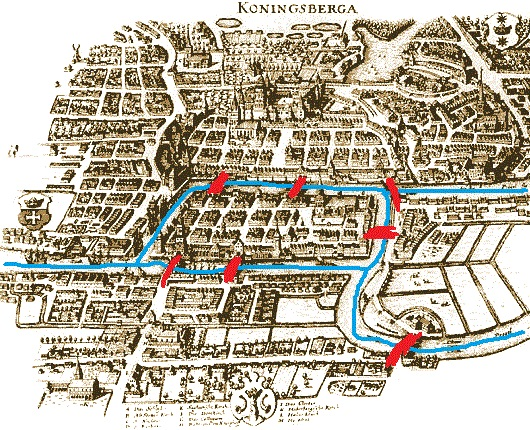
\includegraphics[width=0.7\linewidth,height=\textheight,keepaspectratio]{images/fig_koenigsberg_aa.jpg}

}

\caption{\label{fig-koenigsberg-aa}Mapa de Königsberg con los 7 puentes
y el río Pregel destacados}

\end{figure}%

\begin{figure}

\centering{

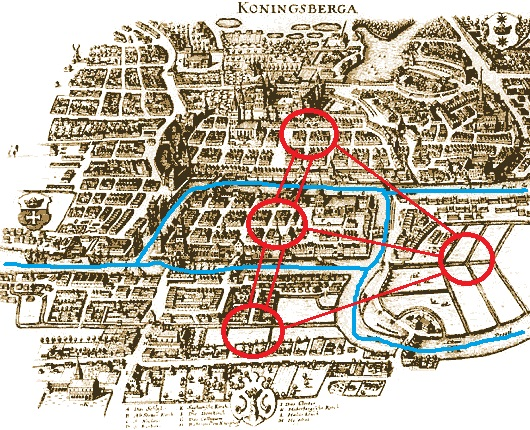
\includegraphics[width=0.7\linewidth,height=\textheight,keepaspectratio]{images/fig_koenigsberg_aaa.jpg}

}

\caption{\label{fig-koenigsberg-aaa}Esquema topológico superpuesto sobre
la mapa de Königsberg (4 regiones y 7 aristas)}

\end{figure}%

El desafío popular consistía en determinar si era posible trazar un
recorrido continuo a pie por la ciudad que cruzase \textbf{cada uno de
los siete puentes exactamente una sola vez} y regresase al punto de
origen. Euler demostró la imposibilidad lógica de dicho recorrido
abstrayendo la posición geográfica real y reduciendo la configuración
espacial a un diagrama puramente topológico formado por nodos (las 4
regiones) y aristas (los 7 puentes), como se observa en la
Figura~\ref{fig-puentes-konigsberg-grafo}.

\begin{figure}

\centering{

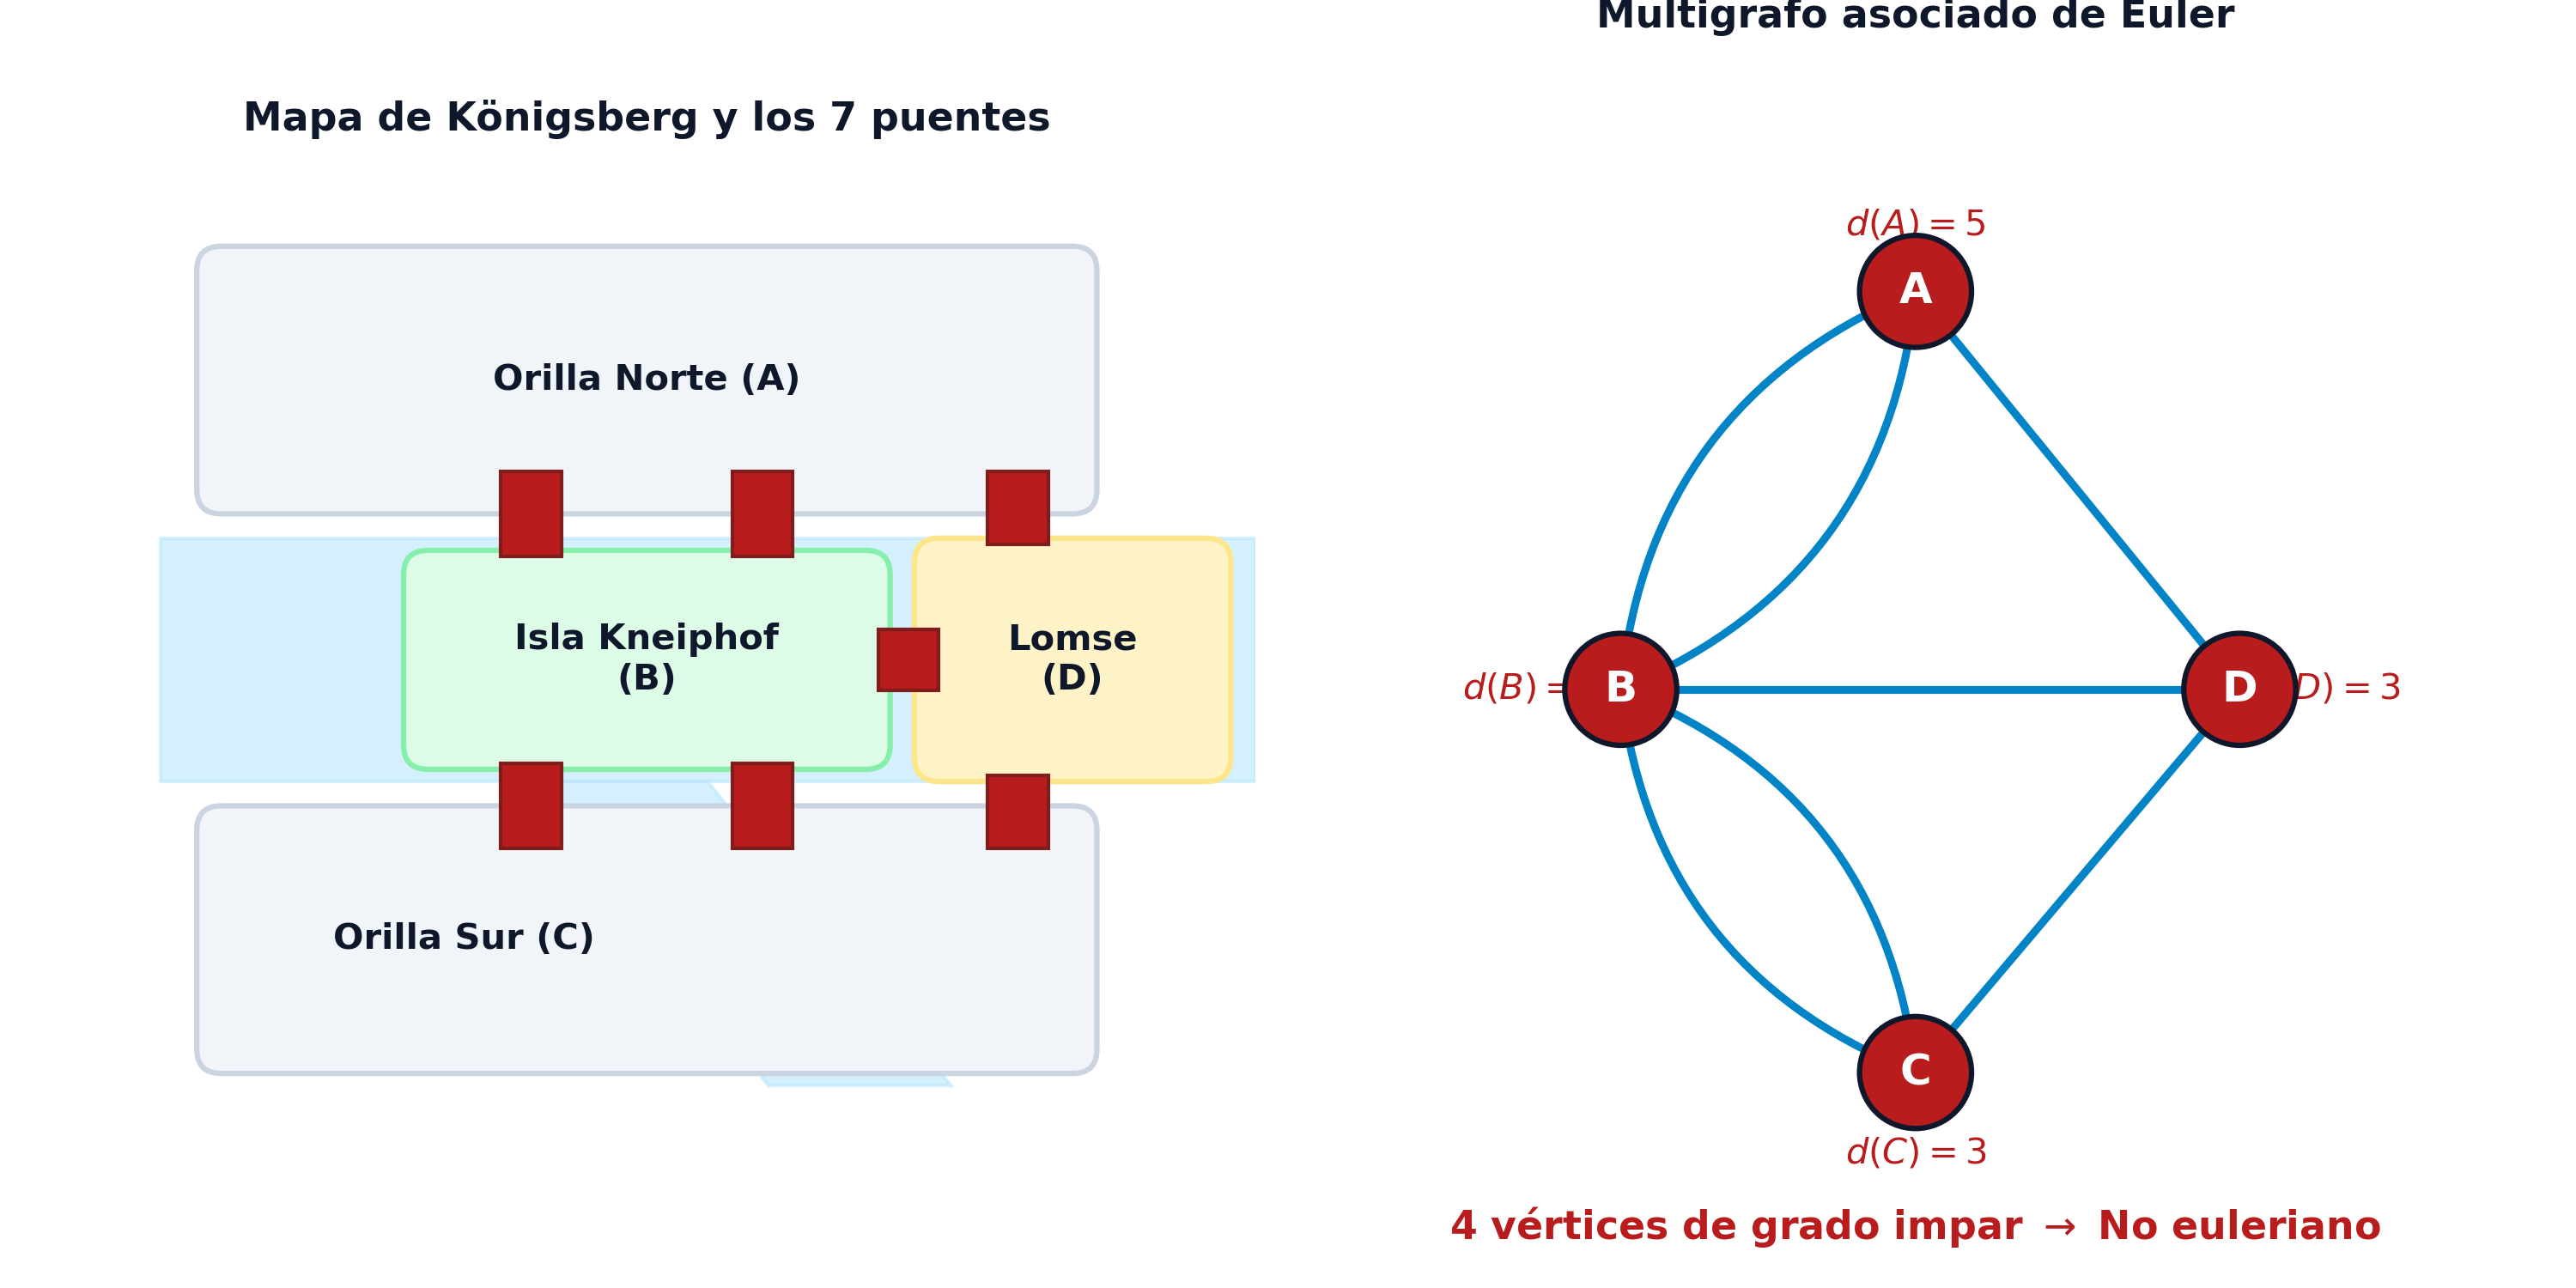
\includegraphics[width=0.5\linewidth,height=\textheight,keepaspectratio]{images/puentes_konigsberg_grafo.png}

}

\caption{\label{fig-puentes-konigsberg-grafo}Grafo multigrafo abstracto
del problema de Königsberg}

\end{figure}%

La genialidad del argumento de Euler radicó en observar que para que un
nodo intermedio admita un paso de entrada y salida sin repetir aristas,
el número de conexiones incidentes en dicho nodo debe ser necesariamente
\textbf{par}. Dado que las cuatro regiones de Königsberg poseen un grado
impar de conexiones (\(d(A)=5, d(B)=3, d(C)=3, d(D)=3\)), el circuito
euleriano deseado resulta matemáticamente imposible.

\begin{center}\rule{0.5\linewidth}{0.5pt}\end{center}

\section{Conceptos fundamentales}\label{conceptos-fundamentales}

El estudio formal de las redes requiere definir con precisión los
elementos constitutivos de un grafo, las relaciones de adyacencia e
incidencia entre sus componentes y las diferentes tipologías
estructurales que adopta la información según la densidad y naturaleza
de sus conexiones.

\subsection{Definición formal de grafos no dirigidos y
dirigidos}\label{definiciuxf3n-formal-de-grafos-no-dirigidos-y-dirigidos}

Desde un punto de vista algebraico y de teoría de conjuntos, un grafo es
un par ordenado formado por un conjunto finitos de elementos discretos
denominados vértices o nodos, y una colección de relaciones que conectan
dichos nodos.

\begin{tcolorbox}[enhanced jigsaw, toprule=.15mm, opacitybacktitle=0.6, coltitle=black, colbacktitle=quarto-callout-note-color!10!white, title=\textcolor{quarto-callout-note-color}{\faInfo}\hspace{0.5em}{Definición: Grafo no dirigido y digrafo}, arc=.35mm, rightrule=.15mm, toptitle=1mm, breakable, bottomtitle=1mm, titlerule=0mm, colback=white, opacityback=0, leftrule=.75mm, colframe=quarto-callout-note-color-frame, left=2mm, bottomrule=.15mm]

\textbf{Grafo No Dirigido} Un \textbf{grafo no dirigido} es un par
\(G = (V, E)\), donde \(V = \{1, 2, \dots, n\}\) representa el conjunto
finito de vértices o nodos (con \(|V| = n\)), y
\(E \subseteq \{\{i, j\} : i, j \in V, i \neq j\}\) denota el conjunto
de \textbf{aristas} no ordenadas (con \(|E| = m\)). Una arista
\(e = \{i, j\}\) representa una relación simétrica entre los nodos \(i\)
y \(j\).

\textbf{Grafo Dirigido o Digrafo} Un \textbf{digrafo} o \textbf{grafo
dirigido} es un par \(G = (V, U)\), donde \(V = \{1, 2, \dots, n\}\)
representa el conjunto de vértices, y \(U \subseteq V \times V\) denota
el conjunto de \textbf{arcos dirigidos} u ordenados. Un arco
\(u = (i, j) \in U\) parte del nodo de origen o cola \(i\) y se dirige
hacia el nodo de destino o cabeza \(j\).

\end{tcolorbox}

Para ilustrar de forma intuitiva estas definiciones, consideremos el
modelado de una red de transporte aéreo internacional representada en la
Figura~\ref{fig-red-vuelos-ejemplo}.

\begin{figure}

\centering{

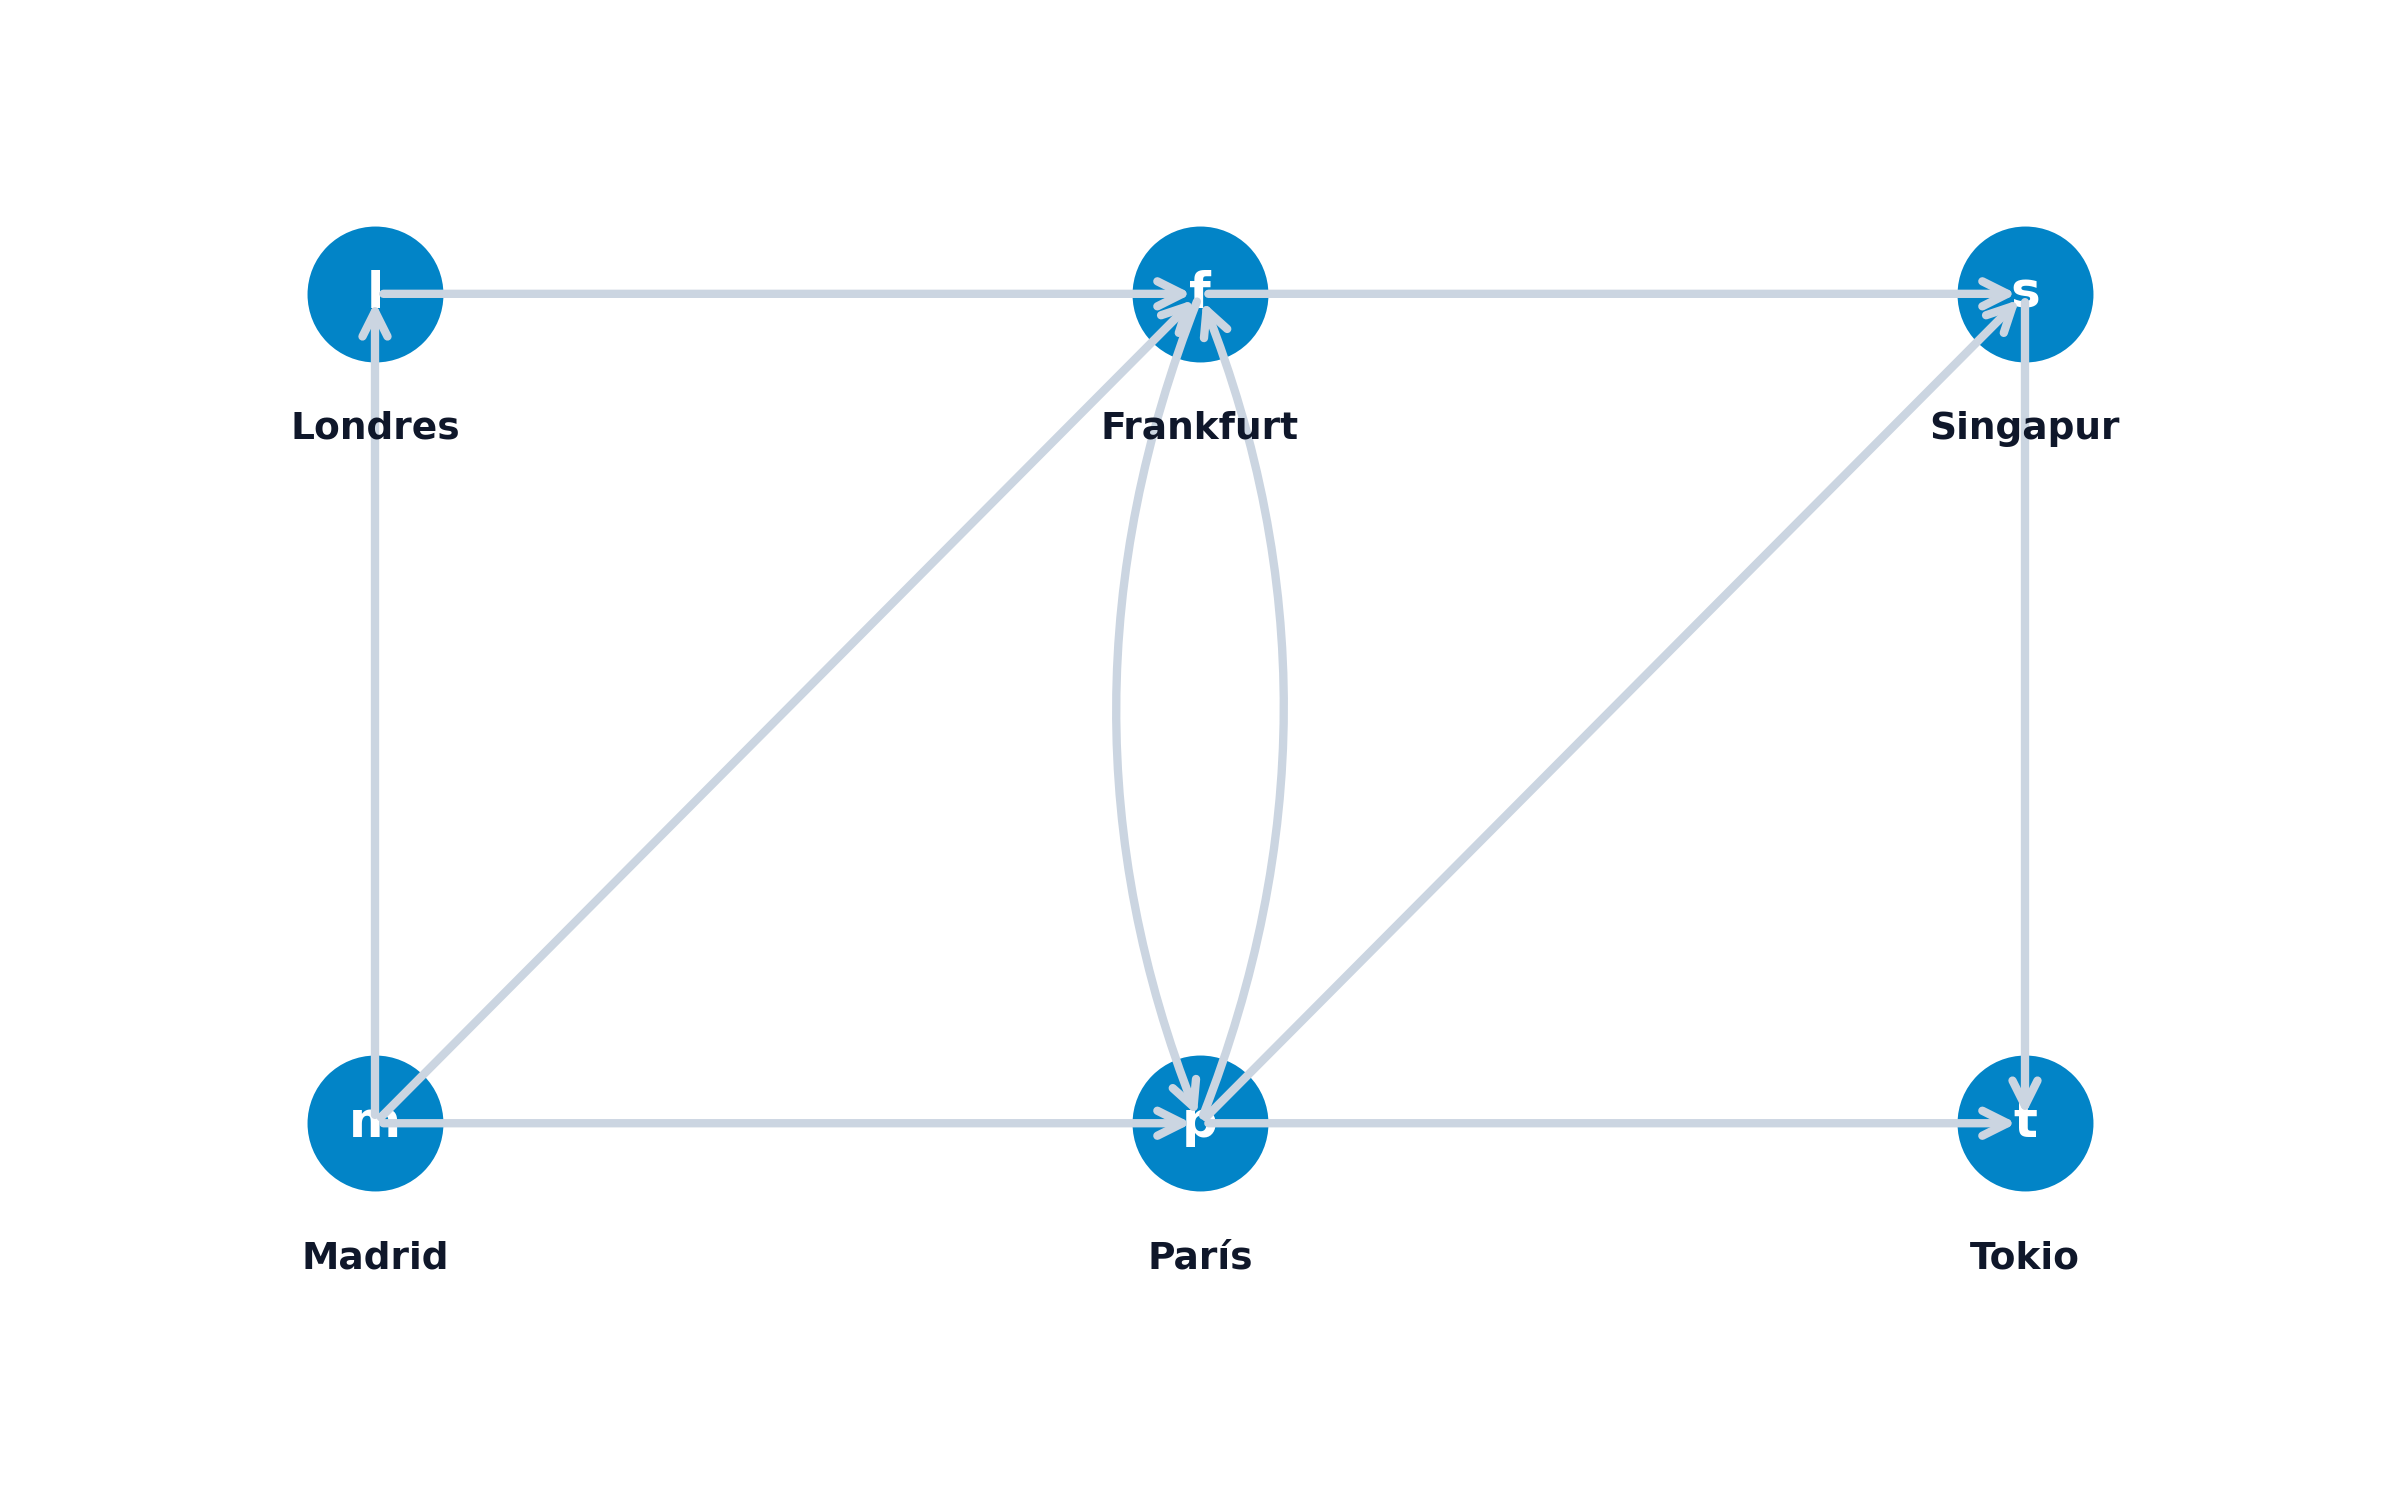
\includegraphics[width=0.75\linewidth,height=\textheight,keepaspectratio]{images/red_vuelos_ejemplo.png}

}

\caption{\label{fig-red-vuelos-ejemplo}Red de vuelos compatibles entre
aeropuertos internacionales representados como digrafo}

\end{figure}%

En la Figura~\ref{fig-red-vuelos-ejemplo}, los nodos representan los
aeropuertos \(V = \{m, l, p, f, s, t\}\) correspondientes a Madrid,
Londres, París, Frankfurt, Singapur y Tokio. Los arcos dirigidos
representan conexiones de vuelo directo de ida sin escala. Nótese que
entre París (\(p\)) y Frankfurt (\(f\)) existen arcos dirigidos
antiparalelos \((p, f)\) y \((f, p)\), lo que permite el tránsito
bidireccional entre ambas capitales.

Por otro lado, la estructura formal de un digrafo abstracto \(G=(V,U)\)
puede incorporar arcos dirigidos simples, arcos antiparalelos y bucles
(arcos que nacen y terminan en el mismo vértice, \((i, i) \in U\)), como
se detalla en la Figura~\ref{fig-digrafo-definicion}.

\begin{figure}

\centering{

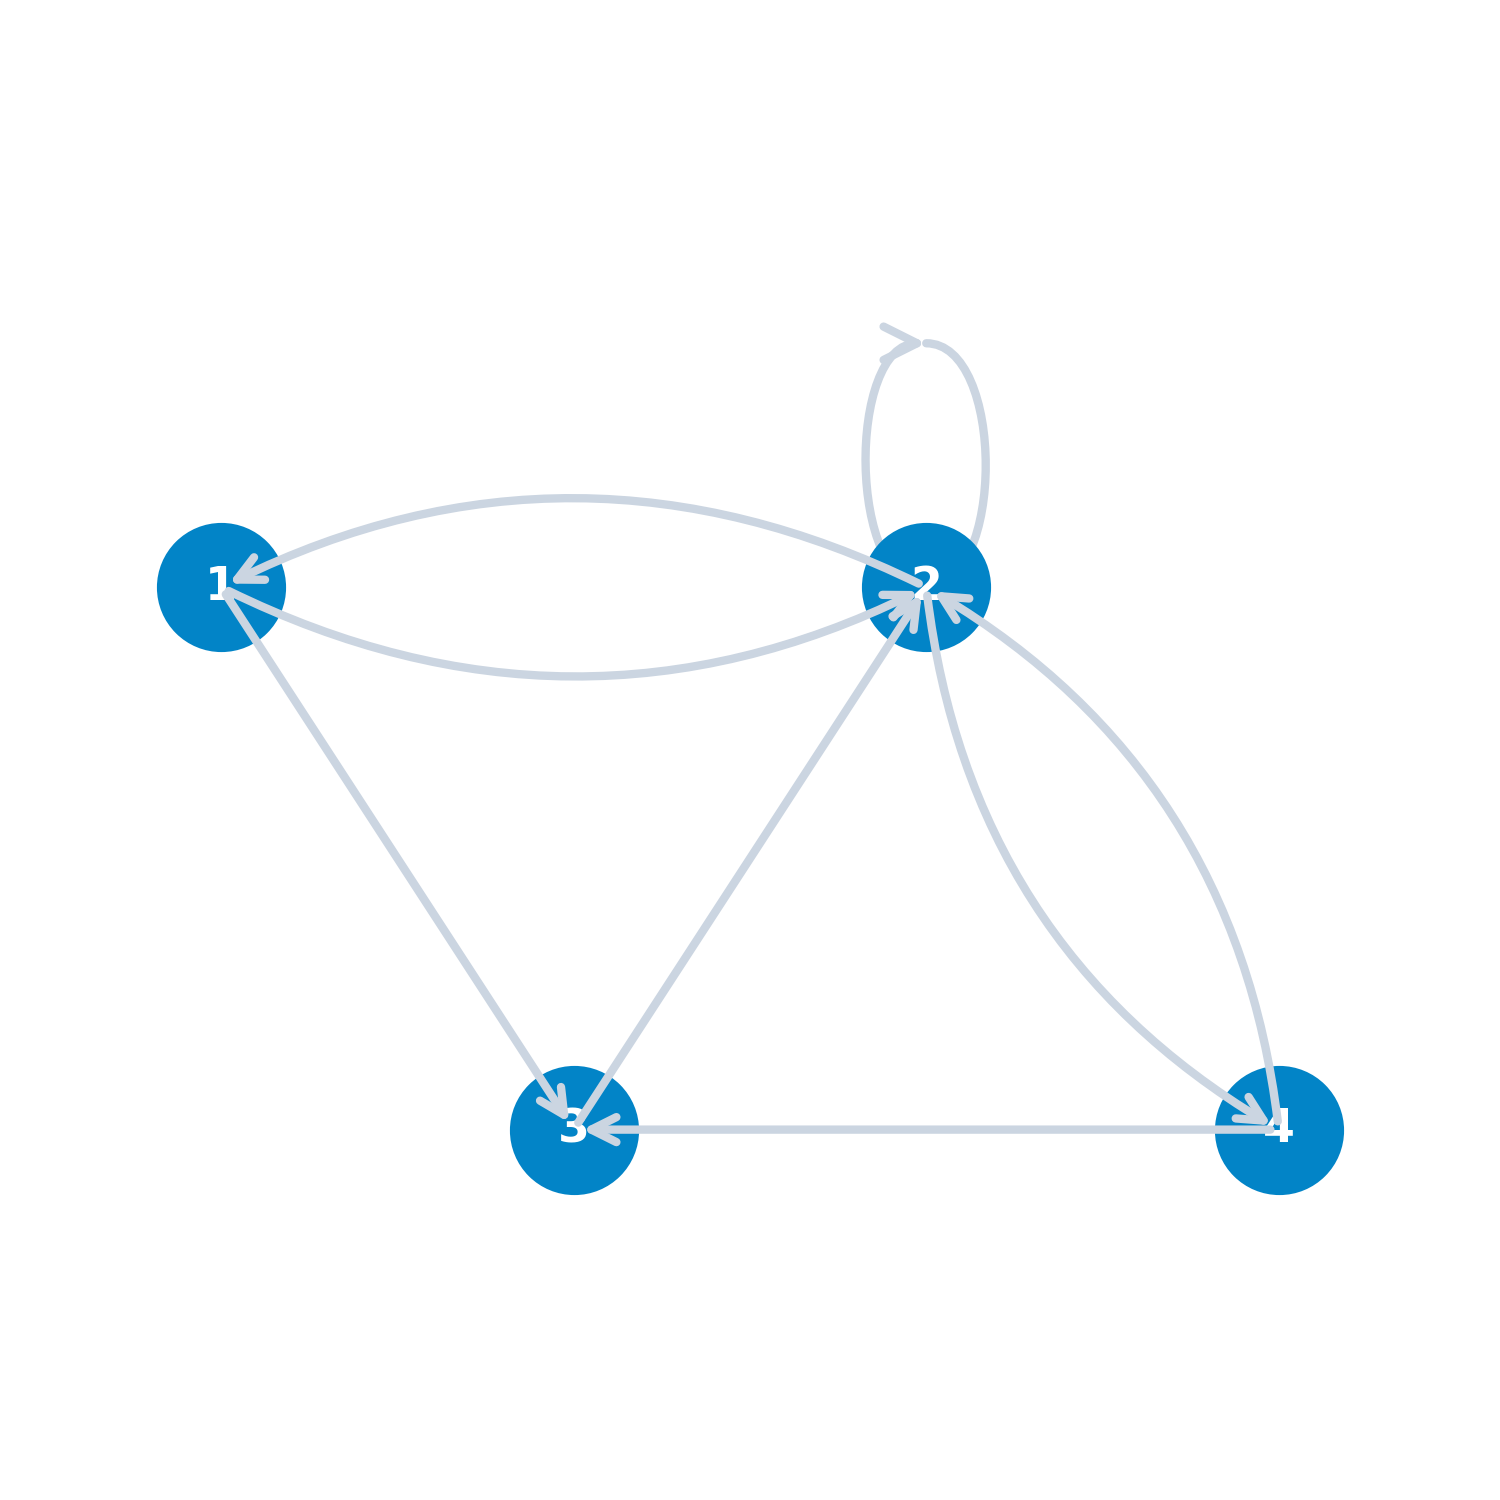
\includegraphics[width=0.5\linewidth,height=\textheight,keepaspectratio]{images/digrafo_definicion.png}

}

\caption{\label{fig-digrafo-definicion}Estructura formal de un digrafo
con arcos ordenados y un bucle autodirigido}

\end{figure}%

\subsection{Vecindades, adyacencia y grados de un
nodo}\label{vecindades-adyacencia-y-grados-de-un-nodo}

Las propiedades locales de un nodo en un grafo se caracterizan
analíticamente a través de sus relaciones de vecindad y su grado de
conexión.

\begin{tcolorbox}[enhanced jigsaw, toprule=.15mm, opacitybacktitle=0.6, coltitle=black, colbacktitle=quarto-callout-note-color!10!white, title=\textcolor{quarto-callout-note-color}{\faInfo}\hspace{0.5em}{Definición: Adyacencia, grados e incidencia}, arc=.35mm, rightrule=.15mm, toptitle=1mm, breakable, bottomtitle=1mm, titlerule=0mm, colback=white, opacityback=0, leftrule=.75mm, colframe=quarto-callout-note-color-frame, left=2mm, bottomrule=.15mm]

Dado un digrafo \(G = (V, U)\) y un nodo \(i \in V\):

\begin{itemize}
\item
  \textbf{Nodos Adyacentes}: Dos nodos \(i, j \in V\) son
  \textbf{adyacentes} si existe una conexión directa entre ellos, es
  decir, si \((i, j) \in U\) o \((j, i) \in U\). El conjunto de todos
  los nodos adyacentes a \(i\) conforma su \textbf{vecindad total}
  \(\Gamma(i) = \Gamma^+(i) \cup \Gamma^-(i)\).
\item
  \textbf{Arcos Adyacentes}: Dos arcos \(u_1, u_2 \in U\) son
  \textbf{adyacentes} cuando comparten al menos un nodo extremo común
  (por ejemplo, los arcos \((1, 2)\) y \((2, 4)\) son adyacentes al
  conectarse en el nodo \(2\)).
\item
  \textbf{Incidencia de un Arco}: Un arco \(u = (i, j) \in U\) es
  \textbf{incidente de salida} en su nodo origen \(i\), e
  \textbf{incidente de entrada} en su nodo destino \(j\).
\end{itemize}

\textbf{Conjunto de Sucesores y Predecesores}

\begin{itemize}
\tightlist
\item
  \textbf{Sucesores}: \(\Gamma^+(i) = \{j \in V : (i, j) \in U\}\),
  conjunto de nodos hacia los que parten arcos desde \(i\).
\item
  \textbf{Predecesores}: \(\Gamma^-(i) = \{j \in V : (j, i) \in U\}\),
  conjunto de nodos desde los que llegan arcos a \(i\).
\item
  \textbf{Vecindad Total}: \(\Gamma(i) = \Gamma^+(i) \cup \Gamma^-(i)\).
\end{itemize}

\textbf{Semigrados y Grado Total}

\begin{itemize}
\tightlist
\item
  \textbf{Semigrado Exterior}: \(d^+(i) = |\Gamma^+(i)|\), número de
  arcos que parten del nodo \(i\).
\item
  \textbf{Semigrado Interior}: \(d^-(i) = |\Gamma^-(i)|\), número de
  arcos que ingresan al nodo \(i\).
\item
  \textbf{Grado Total}: \(d(i) = d^+(i) + d^-(i)\), número total de
  arcos incidentes en el nodo \(i\).
\end{itemize}

Un nodo \(i\) con grado total \(d(i) = 1\) se denomina \textbf{nodo
pendiente} o \textbf{hoja}. Un nodo con \(d(i) = 0\) se denomina
\textbf{nodo aislado}.

\end{tcolorbox}

Como se observa geométricamente en la
Figura~\ref{fig-adyacencia-vecindades}, para el nodo 3 del digrafo, su
conjunto de sucesores es \(\Gamma^+(3)=\{2\}\), su conjunto de
predecesores es \(\Gamma^-(3)=\{1, 4\}\), y su vecindad total combinada
es \(\Gamma(3)=\{1, 2, 4\}\).

\begin{figure}

\centering{

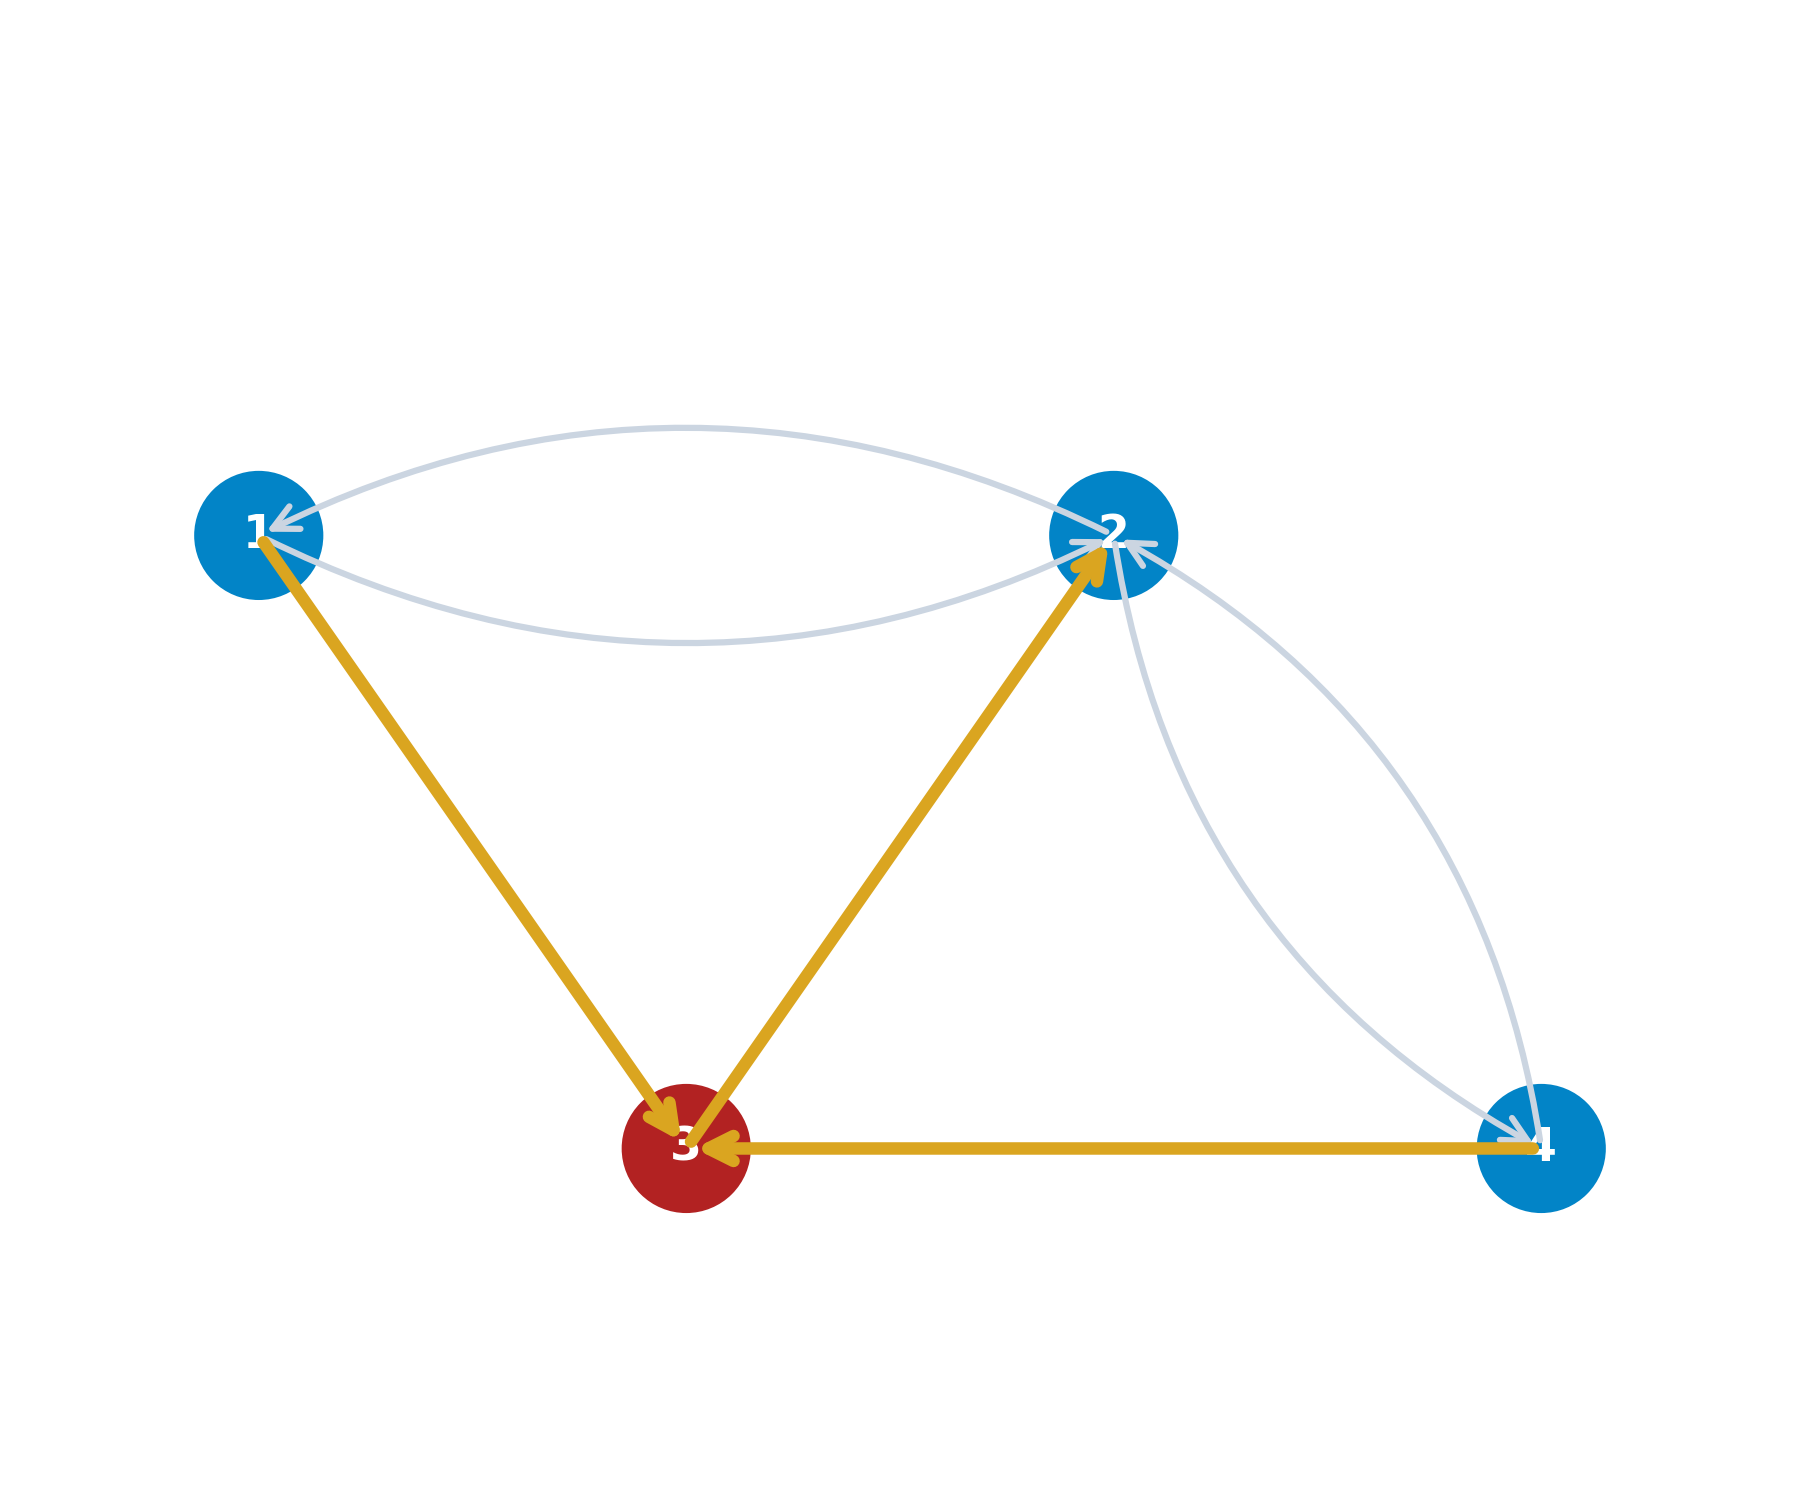
\includegraphics[width=0.6\linewidth,height=\textheight,keepaspectratio]{images/adyacencia_vecindades.png}

}

\caption{\label{fig-adyacencia-vecindades}Adyacencia y vecindades de
sucesores y predecesores para el nodo 3}

\end{figure}%

Asimismo, en la Figura~\ref{fig-grado-nodos} se representa la evaluación
de los semigrados de los nodos de la red, donde el nodo 5 se identifica
como un nodo pendiente al tener un grado total \(d(5)=1\)
(\(d^+(5)=0, d^-(5)=1\)).

\begin{figure}

\centering{

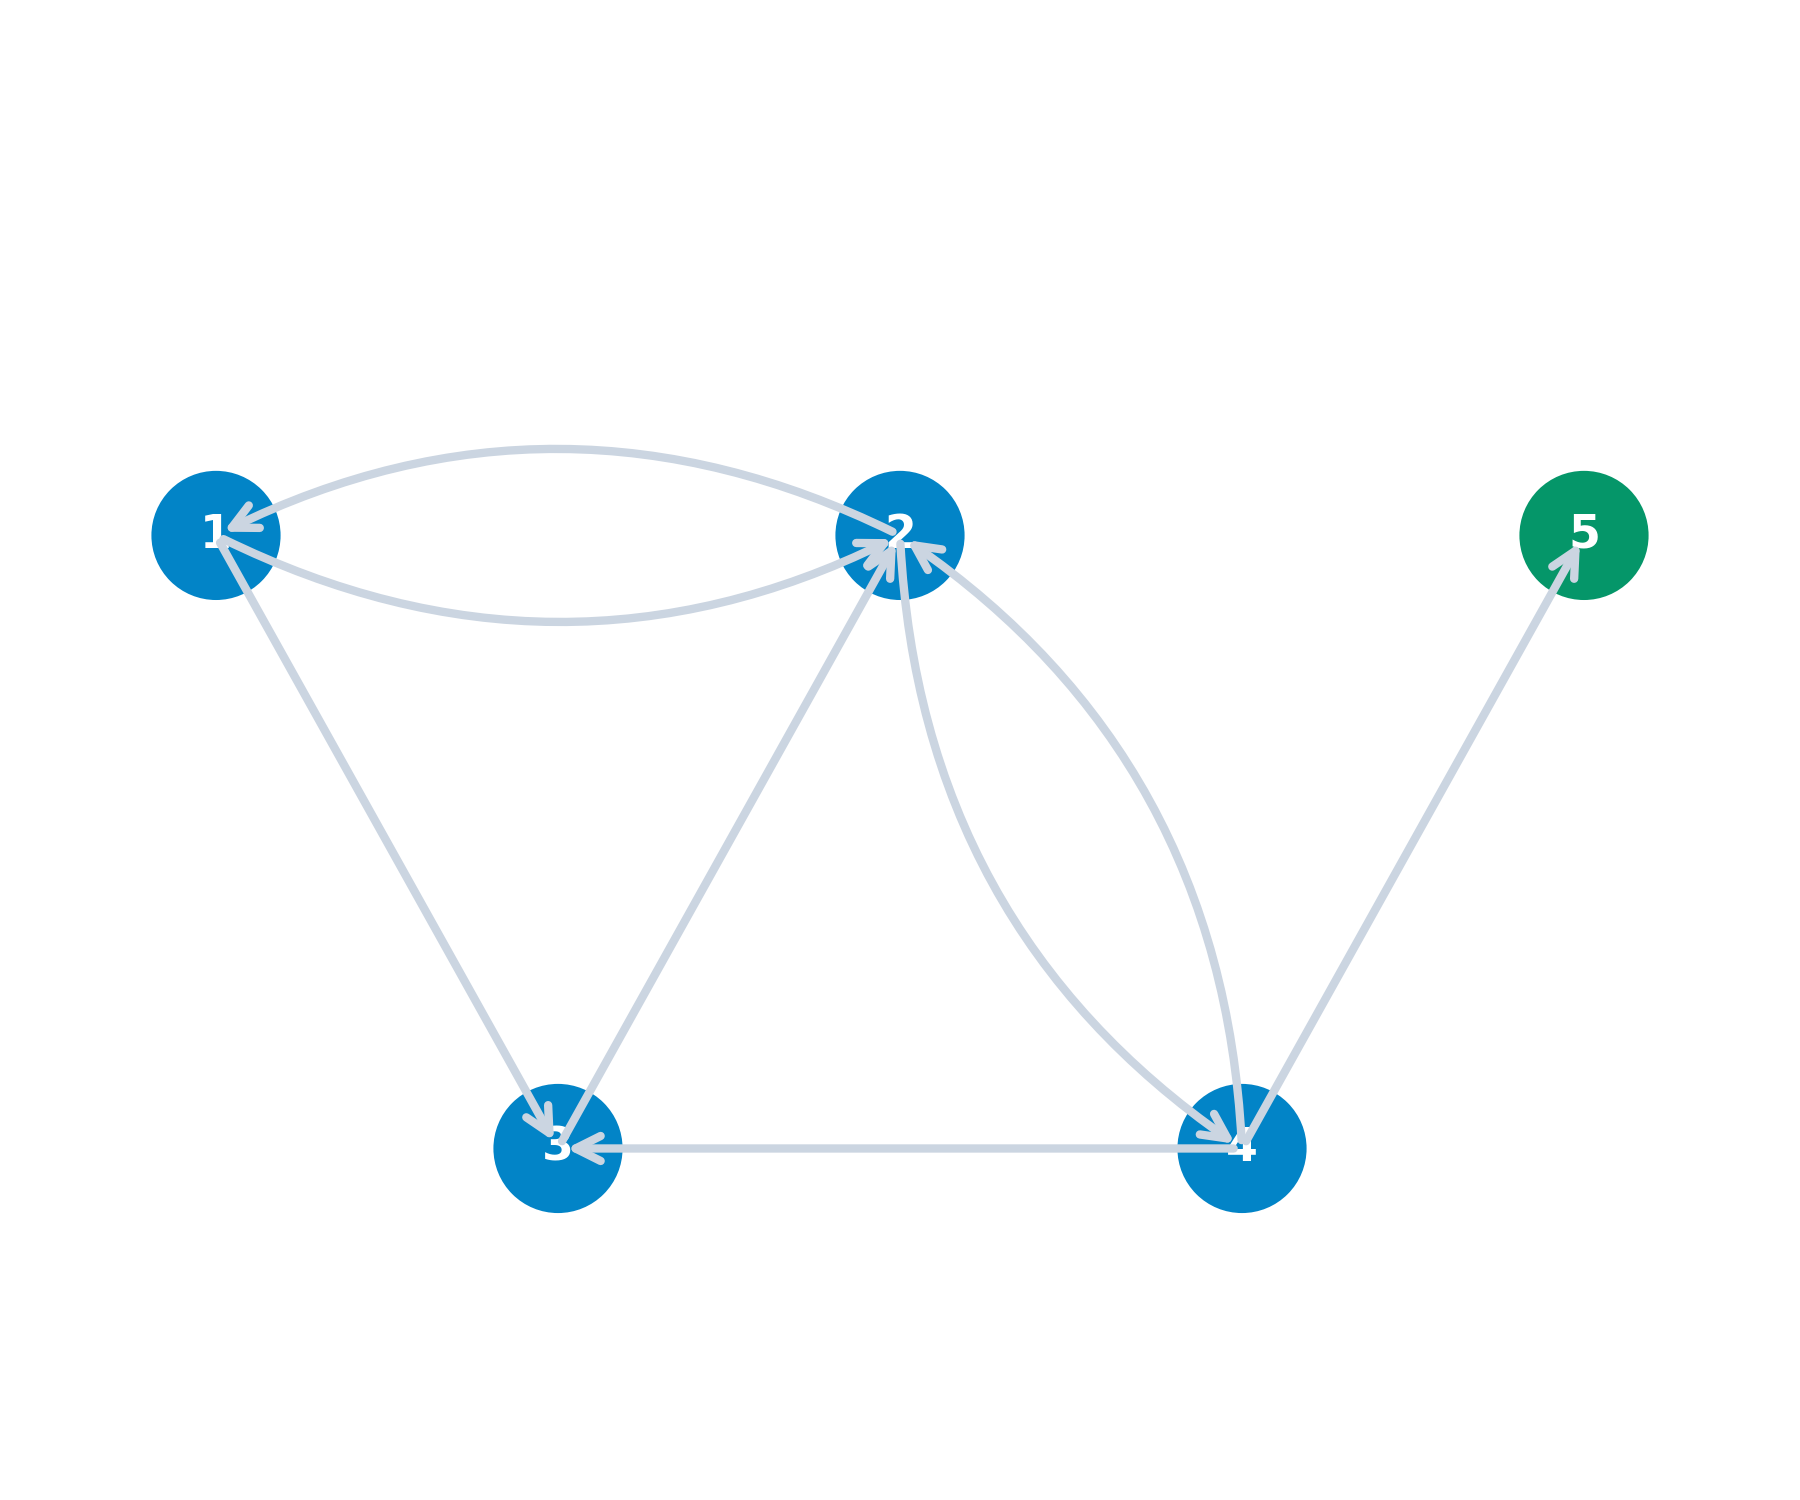
\includegraphics[width=0.6\linewidth,height=\textheight,keepaspectratio]{images/grado_nodos.png}

}

\caption{\label{fig-grado-nodos}Semigrados exterior e interior y
caracterización de nodo pendiente}

\end{figure}%

\begin{tcolorbox}[enhanced jigsaw, toprule=.15mm, opacitybacktitle=0.6, coltitle=black, colbacktitle=quarto-callout-important-color!10!white, title=\textcolor{quarto-callout-important-color}{\faExclamation}\hspace{0.5em}{Teorema de la suma de grados (Handshaking Lemma)}, arc=.35mm, rightrule=.15mm, toptitle=1mm, breakable, bottomtitle=1mm, titlerule=0mm, colback=white, opacityback=0, leftrule=.75mm, colframe=quarto-callout-important-color-frame, left=2mm, bottomrule=.15mm]

En todo grafo no dirigido \(G = (V, E)\) con \(|V| = n\) y \(|E| = m\),
la suma de los grados de todos los vértices es igual al doble del número
total de aristas: \[
\sum_{v \in V} d(v) = 2m
\]

\emph{Demostración}: Cada arista \(e = \{u, v\} \in E\) contribuye
exactamente en \(1\) unidad al grado del nodo \(u\) y en \(1\) unidad al
grado del nodo \(v\). Por consiguiente, al sumar los grados de todos los
nodos en \(V\), cada arista del conjunto \(E\) es contabilizada
exactamente dos veces. \(\blacksquare\)

\end{tcolorbox}

\subsection{Incidencia de conjuntos y
cortes}\label{incidencia-de-conjuntos-y-cortes}

En el estudio de los flujos en redes y la conectividad, resulta esencial
cuantificar los arcos que cruzan la frontera entre dos subconjuntos de
vértices.

\begin{tcolorbox}[enhanced jigsaw, toprule=.15mm, opacitybacktitle=0.6, coltitle=black, colbacktitle=quarto-callout-note-color!10!white, title=\textcolor{quarto-callout-note-color}{\faInfo}\hspace{0.5em}{Definición: Incidencia de un conjunto de nodos}, arc=.35mm, rightrule=.15mm, toptitle=1mm, breakable, bottomtitle=1mm, titlerule=0mm, colback=white, opacityback=0, leftrule=.75mm, colframe=quarto-callout-note-color-frame, left=2mm, bottomrule=.15mm]

Dado un digrafo \(G = (V, U)\) y un subconjunto propio de nodos
\(A \subset V\):

\begin{itemize}
\item
  \textbf{Incidencia Exterior} \(w^+(A)\): Conjunto de arcos que parten
  de \(A\) y finalizan fuera de \(A\): \[
  w^+(A) = \{(i, j) \in U : i \in A, j \in V \setminus A\}
  \]
\item
  \textbf{Incidencia Interior} \(w^-(A)\): Conjunto de arcos que parten
  de fuera de \(A\) e ingresan en \(A\): \[
  w^-(A) = \{(i, j) \in U : i \in V \setminus A, j \in A\}
  \]
\item
  \textbf{Corte} \(w(A)\): Unión de las incidencias exterior e interior:
  \(w(A) = w^+(A) \cup w^-(A)\).
\end{itemize}

\end{tcolorbox}

En la Figura~\ref{fig-incidencia-corte-conjuntos} se ilustra la
aplicación práctica de esta definición sobre una red de 5 nodos
seleccionando el subconjunto de nodos \(A = \{2, 3\}\) (resaltados en
color rojo ladrillo).

Para el subconjunto de nodos \(A = \{2, 3\}\), la evaluación analítica
de las incidencias y el corte resulta:

\[
\begin{aligned}
\textcolor{firebrick}{w^+(A) = w^+(\{2,3\})} &= \textcolor{firebrick}{\{(2,4), (3,1), (3,5)\}} \\
\textcolor{dodgerblue}{w^-(A) = w^-(\{2,3\})} &= \textcolor{dodgerblue}{\{(1,2), (4,3)\}} \\
w(A) = w(\{2,3\}) &= \{\textcolor{dodgerblue}{(1,2)}, \textcolor{firebrick}{(2,4)}, \textcolor{firebrick}{(3,1)}, \textcolor{firebrick}{(3,5)}, \textcolor{dodgerblue}{(4,3)}\}
\end{aligned}
\]

Como se refleja visualmente en el sistema de ecuaciones y en la figura:
El corte \(w(A)\) cuantifica la frontera que separa el subconjunto \(A\)
del resto de la red. La incidencia exterior
\(\textcolor{firebrick}{w^+(A)}\) agrupa los arcos salientes que nacen
en \(A\) y se dirigen hacia los nodos exteriores, mientras que la
incidencia interior \(\textcolor{dodgerblue}{w^-(A)}\) agrupa los arcos
entrantes desde el exterior hacia \(A\). El corte total combina ambas
incidencias, diferenciando los arcos que cruzan dicha frontera de
aquellos que permanecen internos a \(A\) o externos al mismo.

\begin{figure}

\centering{

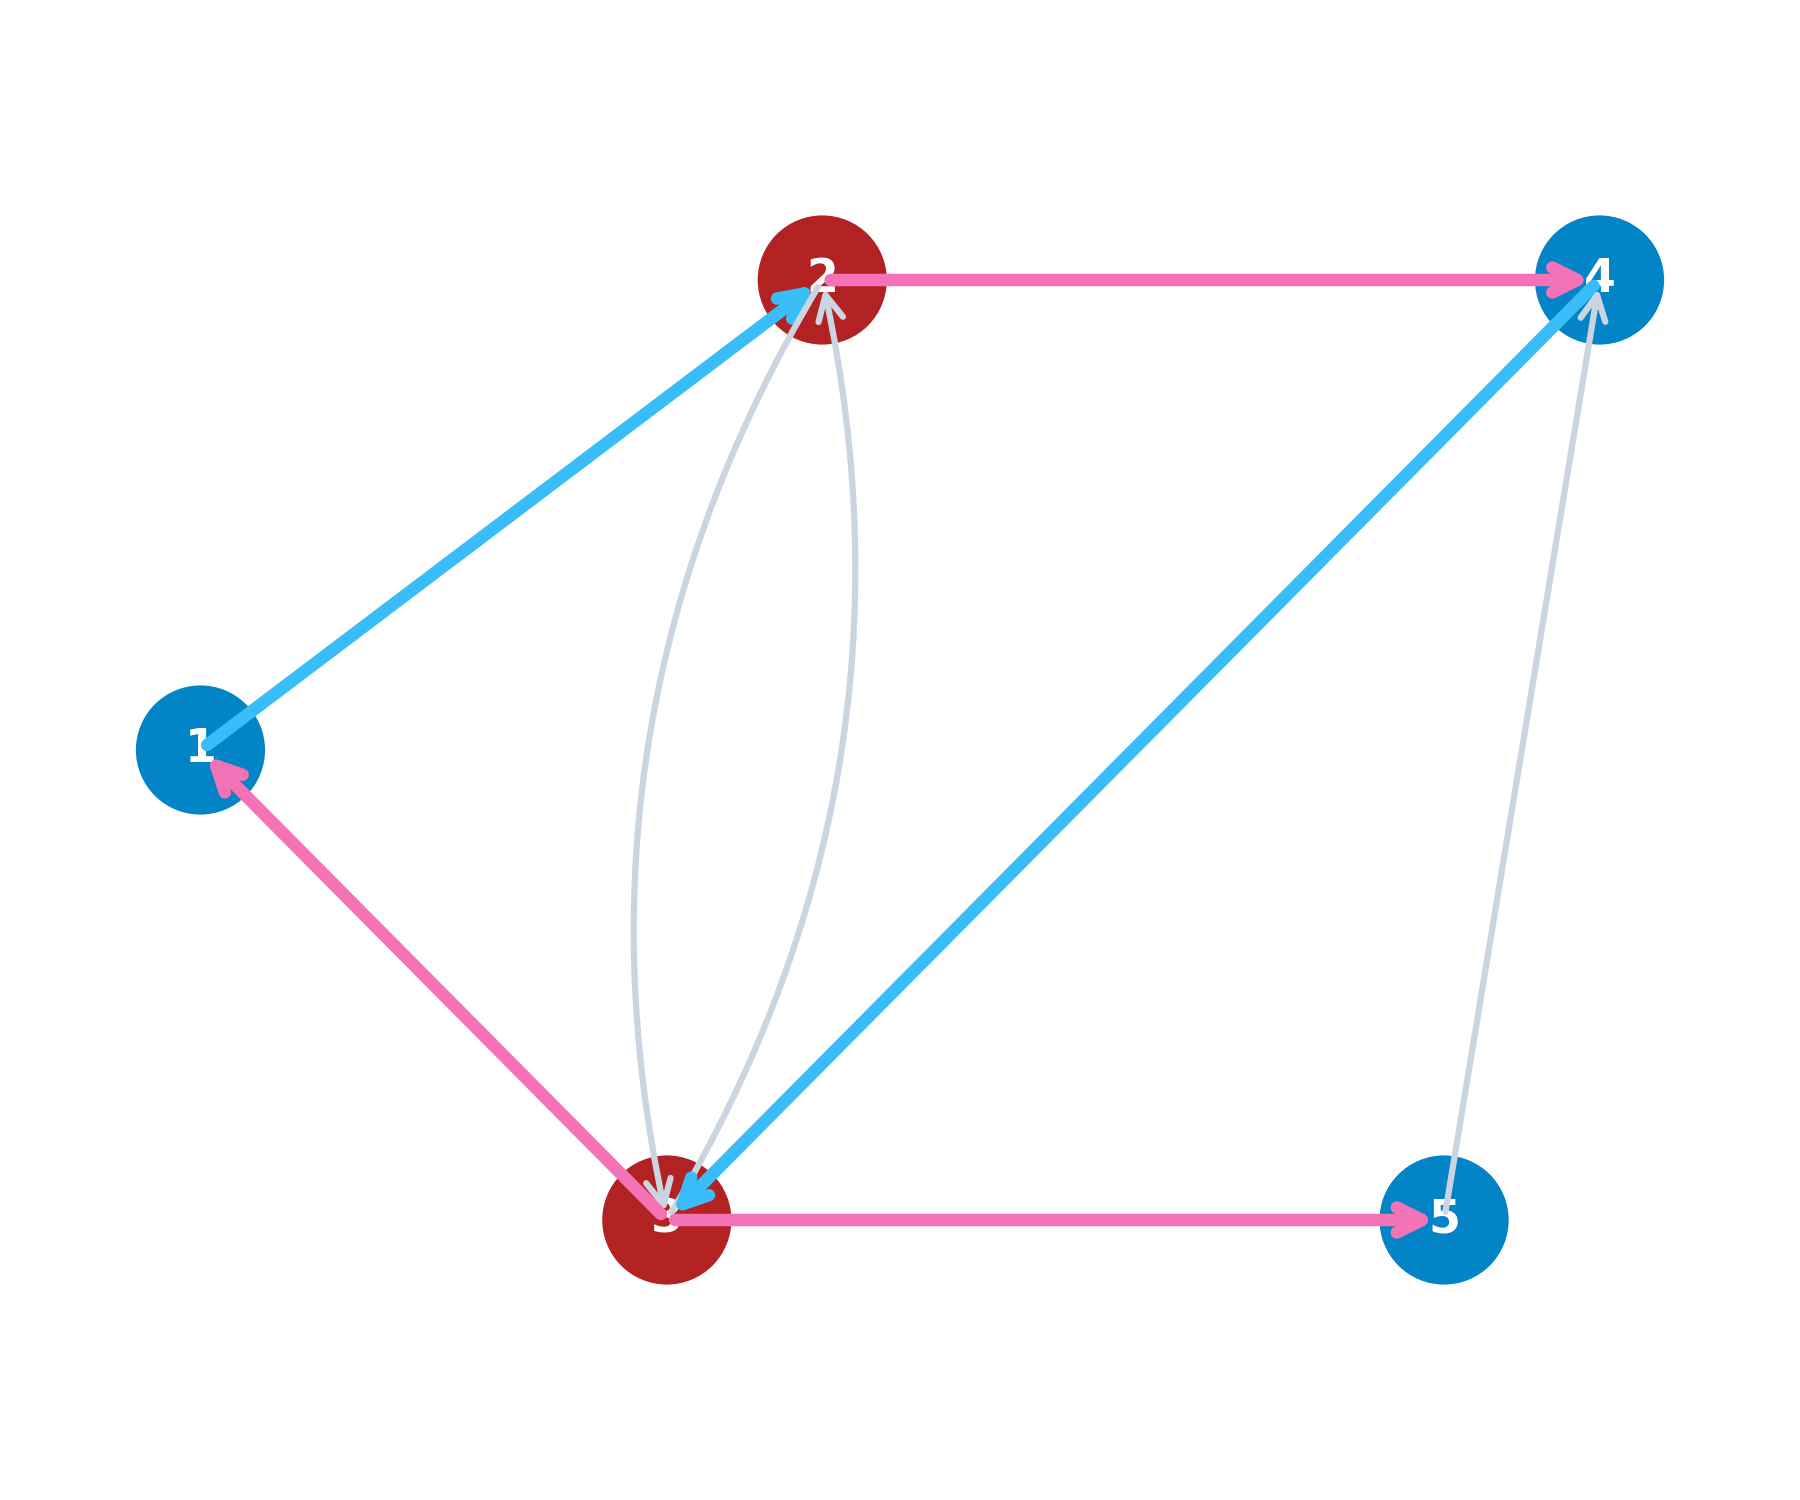
\includegraphics[width=0.6\linewidth,height=\textheight,keepaspectratio]{images/incidencia_corte_conjuntos.png}

}

\caption{\label{fig-incidencia-corte-conjuntos}Incidencia e incidencia
de corte para el subconjunto de nodos A=\{2,3\}}

\end{figure}%

\subsection{Tipología de grafos: multigrafos, grafos completos,
subgrafos y grafos
parciales}\label{tipologuxeda-de-grafos-multigrafos-grafos-completos-subgrafos-y-grafos-parciales}

El modelado formal de sistemas mediante teoría de grafos requiere
clasificar las redes según la multiplicidad de sus relaciones, la
densidad de sus conexiones y las propiedades de sus subestructuras
asociadas.

\begin{tcolorbox}[enhanced jigsaw, toprule=.15mm, opacitybacktitle=0.6, coltitle=black, colbacktitle=quarto-callout-note-color!10!white, title=\textcolor{quarto-callout-note-color}{\faInfo}\hspace{0.5em}{Definición: Multigrafos, multiplicidad y p-grafos}, arc=.35mm, rightrule=.15mm, toptitle=1mm, breakable, bottomtitle=1mm, titlerule=0mm, colback=white, opacityback=0, leftrule=.75mm, colframe=quarto-callout-note-color-frame, left=2mm, bottomrule=.15mm]

Dado un conjunto de vértices \(V\):

\begin{itemize}
\item
  \textbf{Multigrafo / Multidigrafo}: Un \textbf{multigrafo}
  \(G = (V, E)\) (o \textbf{multidigrafo} \(G = (V, U)\)) es una
  estructura matemática que admite la presencia de múltiples aristas o
  arcos en paralelo entre un mismo par de vértices.
\item
  \textbf{Multiplicidad}: Indica el número exacto de conexiones
  repetidas en paralelo entre dos vértices dados.
\item
  \textbf{\(p\)-Grafo}: Se define como un multigrafo en el que la máxima
  multiplicidad de cualquier arista es exactamente \(p\), no existiendo
  pares de nodos conectados por más de \(p\) aristas.
\end{itemize}

\end{tcolorbox}

En aplicaciones reales de transporte e infraestructuras, la presencia de
aristas múltiples permite representar canalizaciones paralelas o rutas
de autobús duplicadas entre dos mismas terminales. Como se ilustra en la
Figura~\ref{fig-multigrafos-pgrafos}, se presenta una red compuesta por
4 vértices \(\{a, b, c, d\}\) donde los pares \(\{a, b\}\) y
\(\{c, d\}\) disponen de 3 conexiones en paralelo cada uno,
constituyendo formalmente un \(3\)-grafo.

\begin{figure}

\centering{

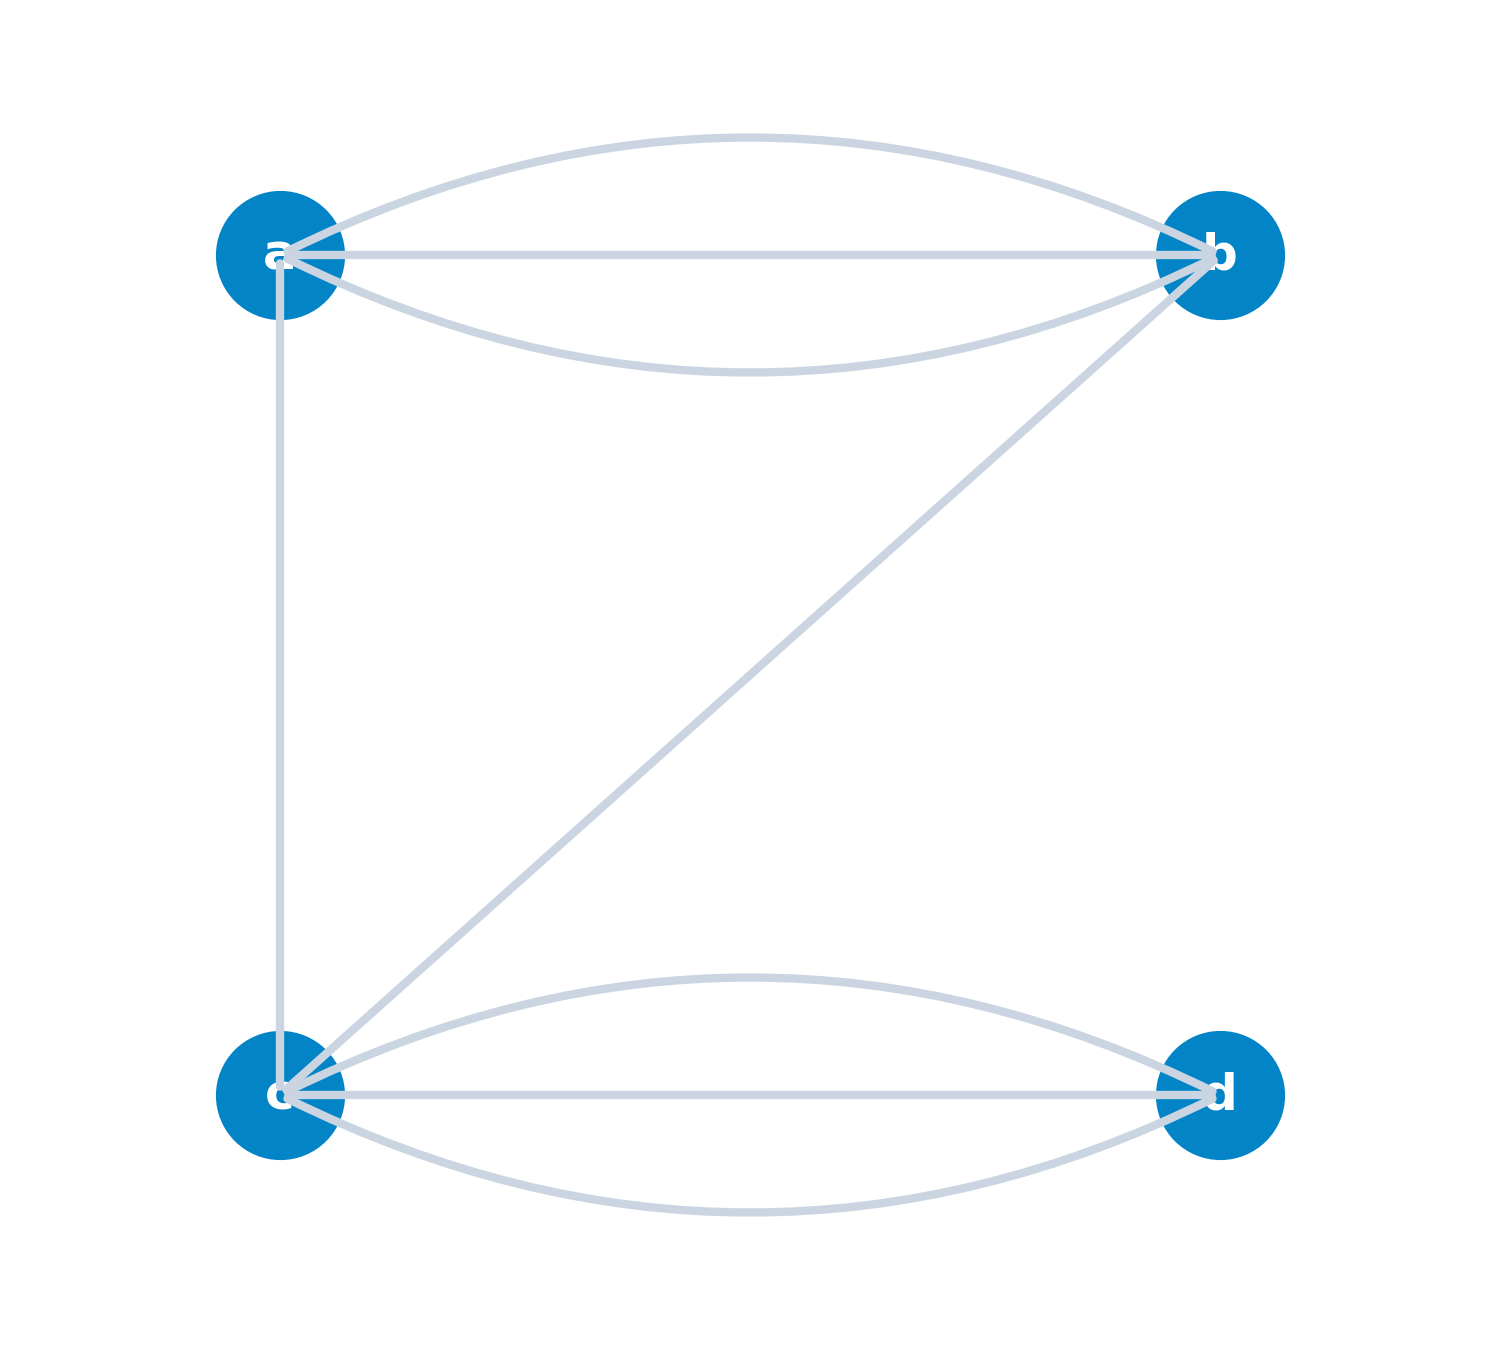
\includegraphics[width=0.55\linewidth,height=\textheight,keepaspectratio]{images/multigrafos_pgrafos.png}

}

\caption{\label{fig-multigrafos-pgrafos}Ejemplo de multigrafo y 3-grafo
con aristas múltiples de multiplicidad 3}

\end{figure}%

Cuando una red carece de bucles y no presenta aristas paralelas, se dice
que es un \textbf{grafo simple}. En el extremo opuesto de máxima
conectividad se sitúan las redes completas.

\begin{tcolorbox}[enhanced jigsaw, toprule=.15mm, opacitybacktitle=0.6, coltitle=black, colbacktitle=quarto-callout-note-color!10!white, title=\textcolor{quarto-callout-note-color}{\faInfo}\hspace{0.5em}{Definición: Grafos simples, completos y clanes}, arc=.35mm, rightrule=.15mm, toptitle=1mm, breakable, bottomtitle=1mm, titlerule=0mm, colback=white, opacityback=0, leftrule=.75mm, colframe=quarto-callout-note-color-frame, left=2mm, bottomrule=.15mm]

Sea \(G = (V, E)\) un grafo no dirigido de \(n = |V|\) vértices:

\begin{itemize}
\item
  \textbf{Grafo Simple}: Estructura de multiplicidad 1 desprovista de
  autodirecciones o bucles \((i, i)\). De forma análoga se define un
  \textbf{digrafo simple}.
\item
  \textbf{Grafo Completo}: Grafo en el que todo par de vértices
  distintos se encuentra conectado por una arista:
  \(\{i, j\} \in E, \forall i \neq j\).
\item
  \textbf{Digrafo Completo}: Digrafo \(G = (V, U)\) donde para todo par
  de nodos distintos \(i \neq j\), la ausencia de arco en un sentido
  implica la existencia obligatoria del arco inverso:
  \((i, j) \notin U \implies (j, i) \in U\).
\item
  \textbf{Clan \(K_n\) (Clique)}: Grafo simple y completo de \(n\)
  vértices. Contiene exactamente \(m = \binom{n}{2} = \frac{n(n-1)}{2}\)
  aristas.
\end{itemize}

\end{tcolorbox}

La distinción entre la completitud en digrafos y en grafos no dirigidos
resulta fundamental en el análisis de redes de transmisión. En un
digrafo completo, la conectividad está garantizada en al menos uno de
los dos sentidos para cada par de nodos. Como se observa en la
Figura~\ref{fig-digrafo-completo}, sobre 4 nodos \(\{a, b, c, d\}\), la
pareja \((a, c)\) está conectada únicamente mediante el arco dirigido
unidireccional \((a, c)\), cumpliendo estrictamente la condición de
completitud orientada.

\begin{figure}

\centering{

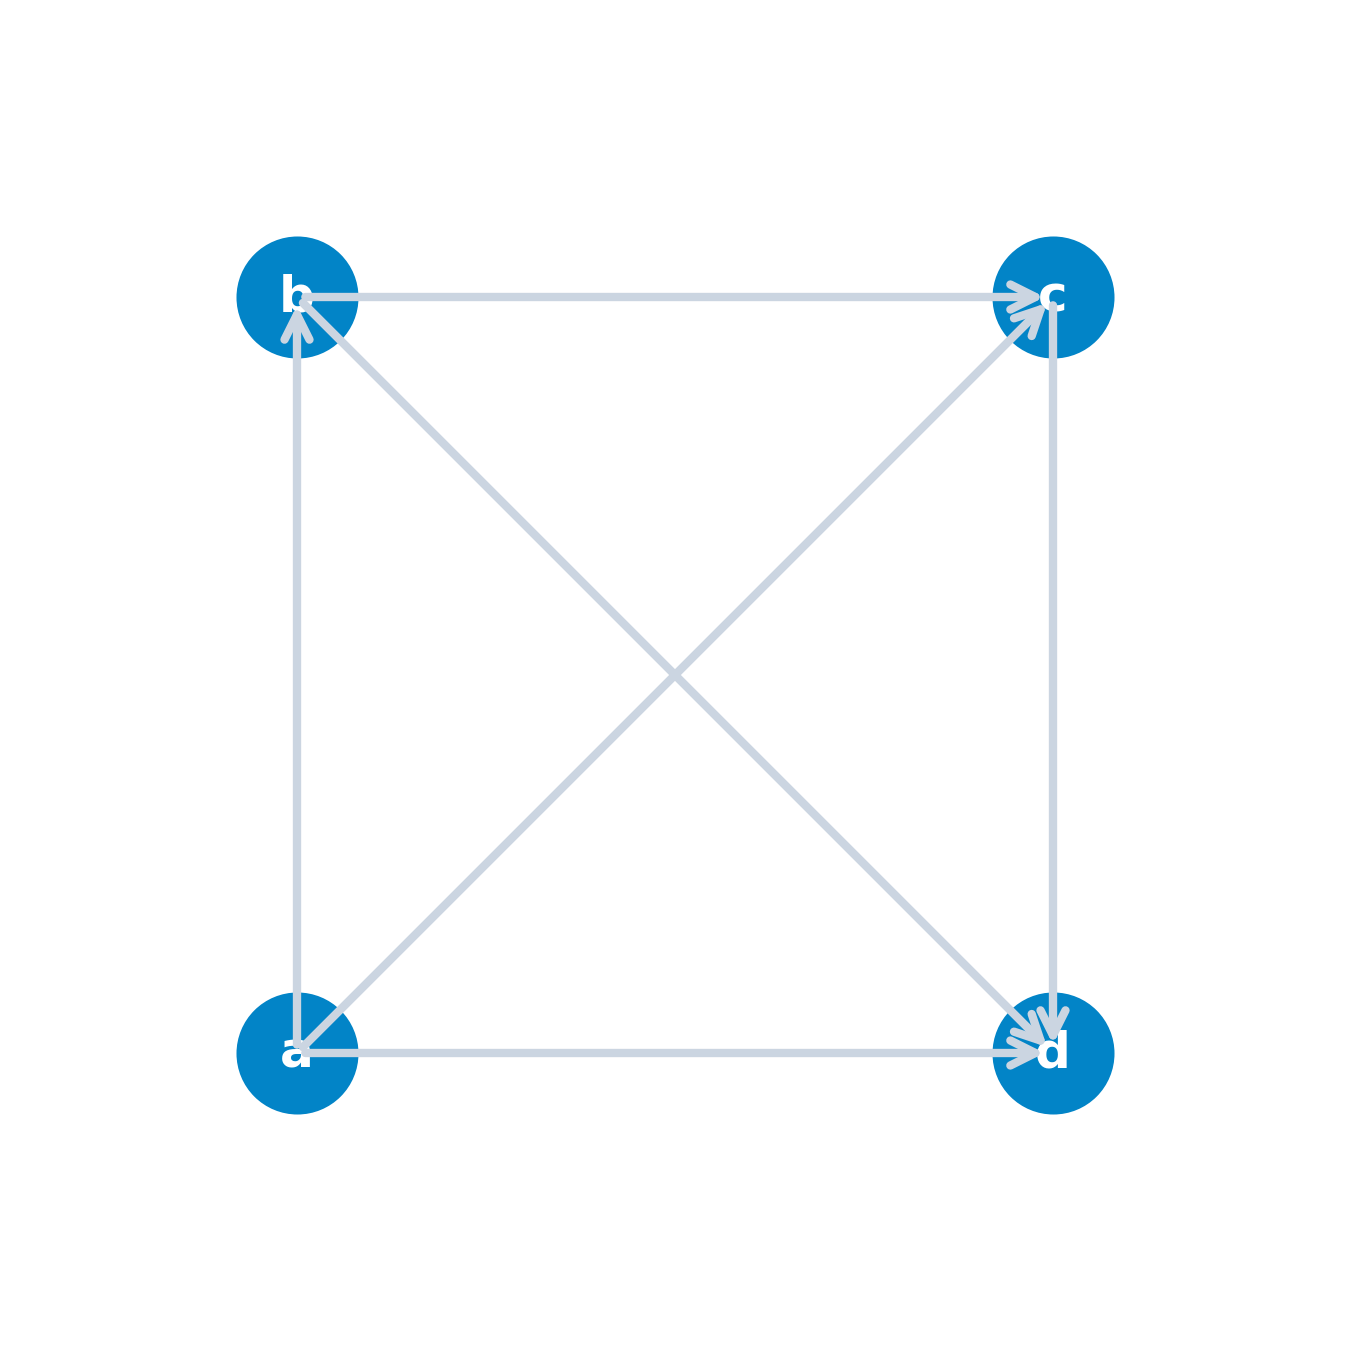
\includegraphics[width=0.45\linewidth,height=\textheight,keepaspectratio]{images/digrafo_completo_ejemplo.png}

}

\caption{\label{fig-digrafo-completo}Digrafo completo sobre 4 nodos con
6 arcos dirigidos}

\end{figure}%

Por su parte, cuando la simetría es total y cada vértice se comunica
bidireccionalmente con todos los demás, la estructura recibe el nombre
de \textbf{clan} o \emph{clique}, denotado por \(K_n\). En la
Figura~\ref{fig-clan-k4} se representa el clan \(K_4\), que integra 6
aristas conectando sus 4 vértices.

\begin{figure}

\centering{

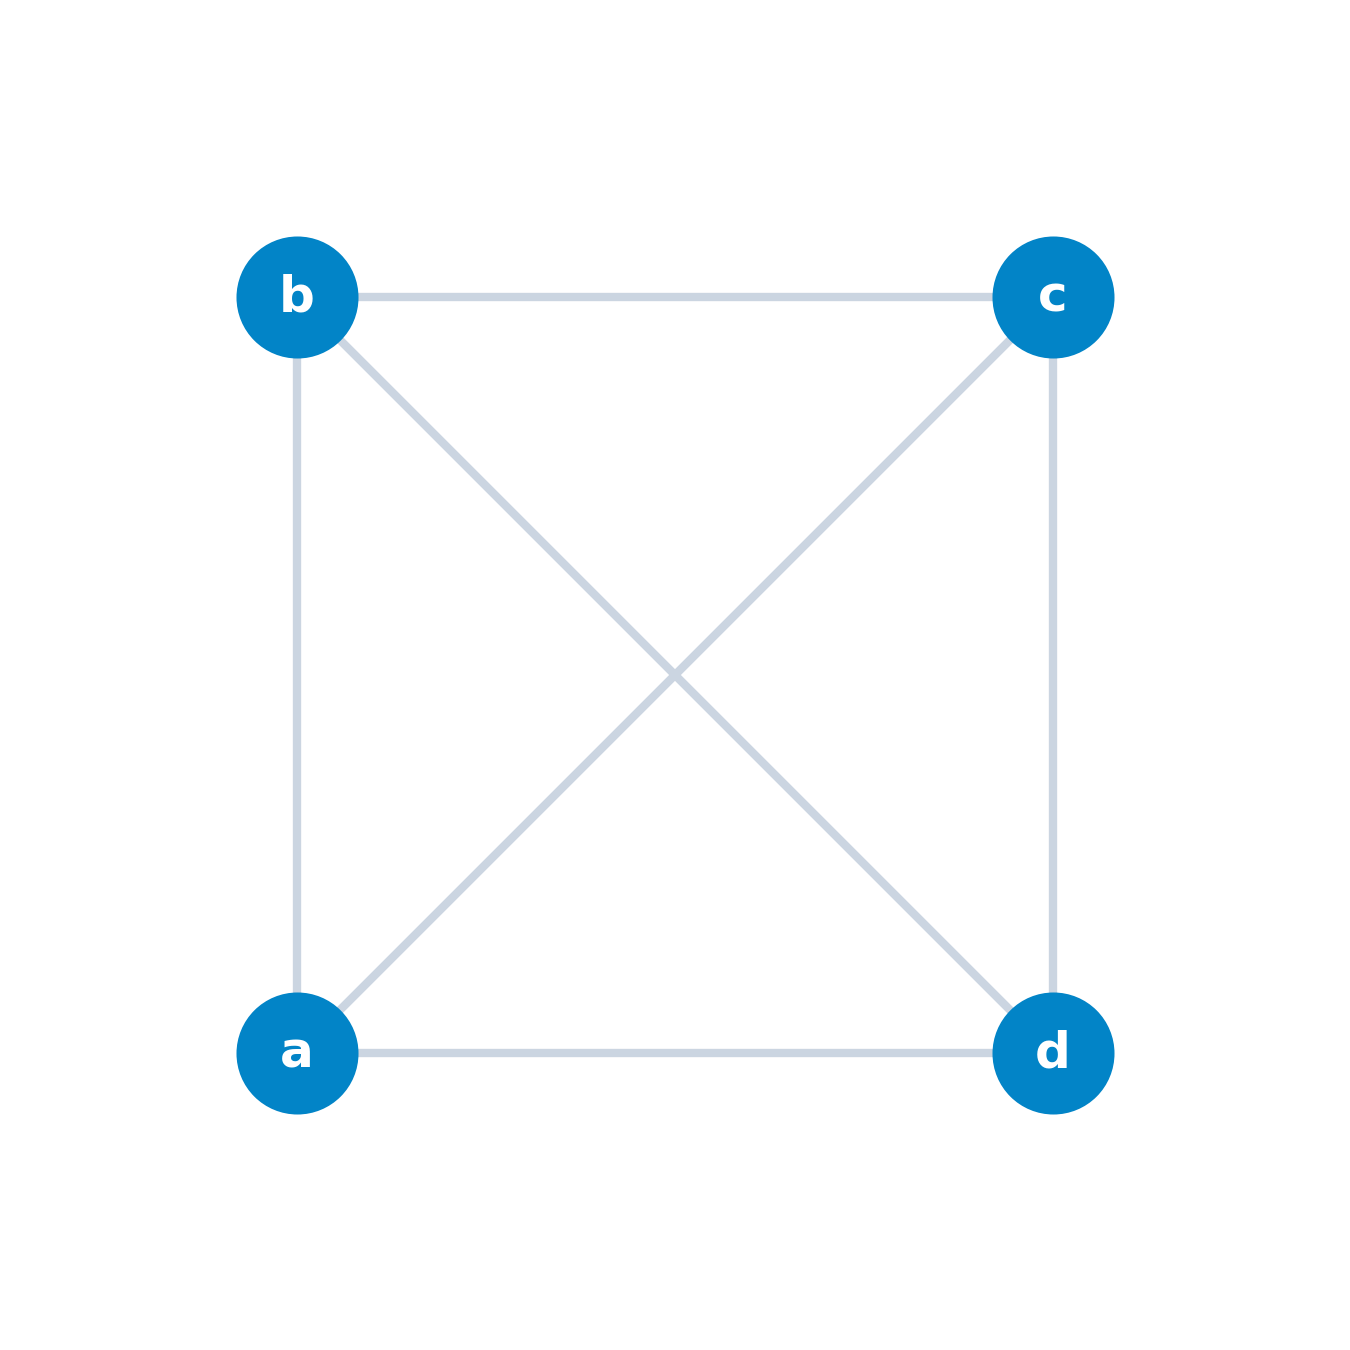
\includegraphics[width=0.4\linewidth,height=\textheight,keepaspectratio]{images/clan_k4_ejemplo.png}

}

\caption{\label{fig-clan-k4}Clan K4 simple completo sobre 4 vértices con
6 aristas}

\end{figure}%

Al incrementar la dimensión a \(n=5\) vértices, el número de conexiones
necesarias para mantener la completitud crece de forma cuadrática
alcanzando las \(m = \frac{5 \times 4}{2} = 10\) aristas, tal como se
muestra en la Figura~\ref{fig-clan-k5} para el clan \(K_5\).

\begin{figure}

\centering{

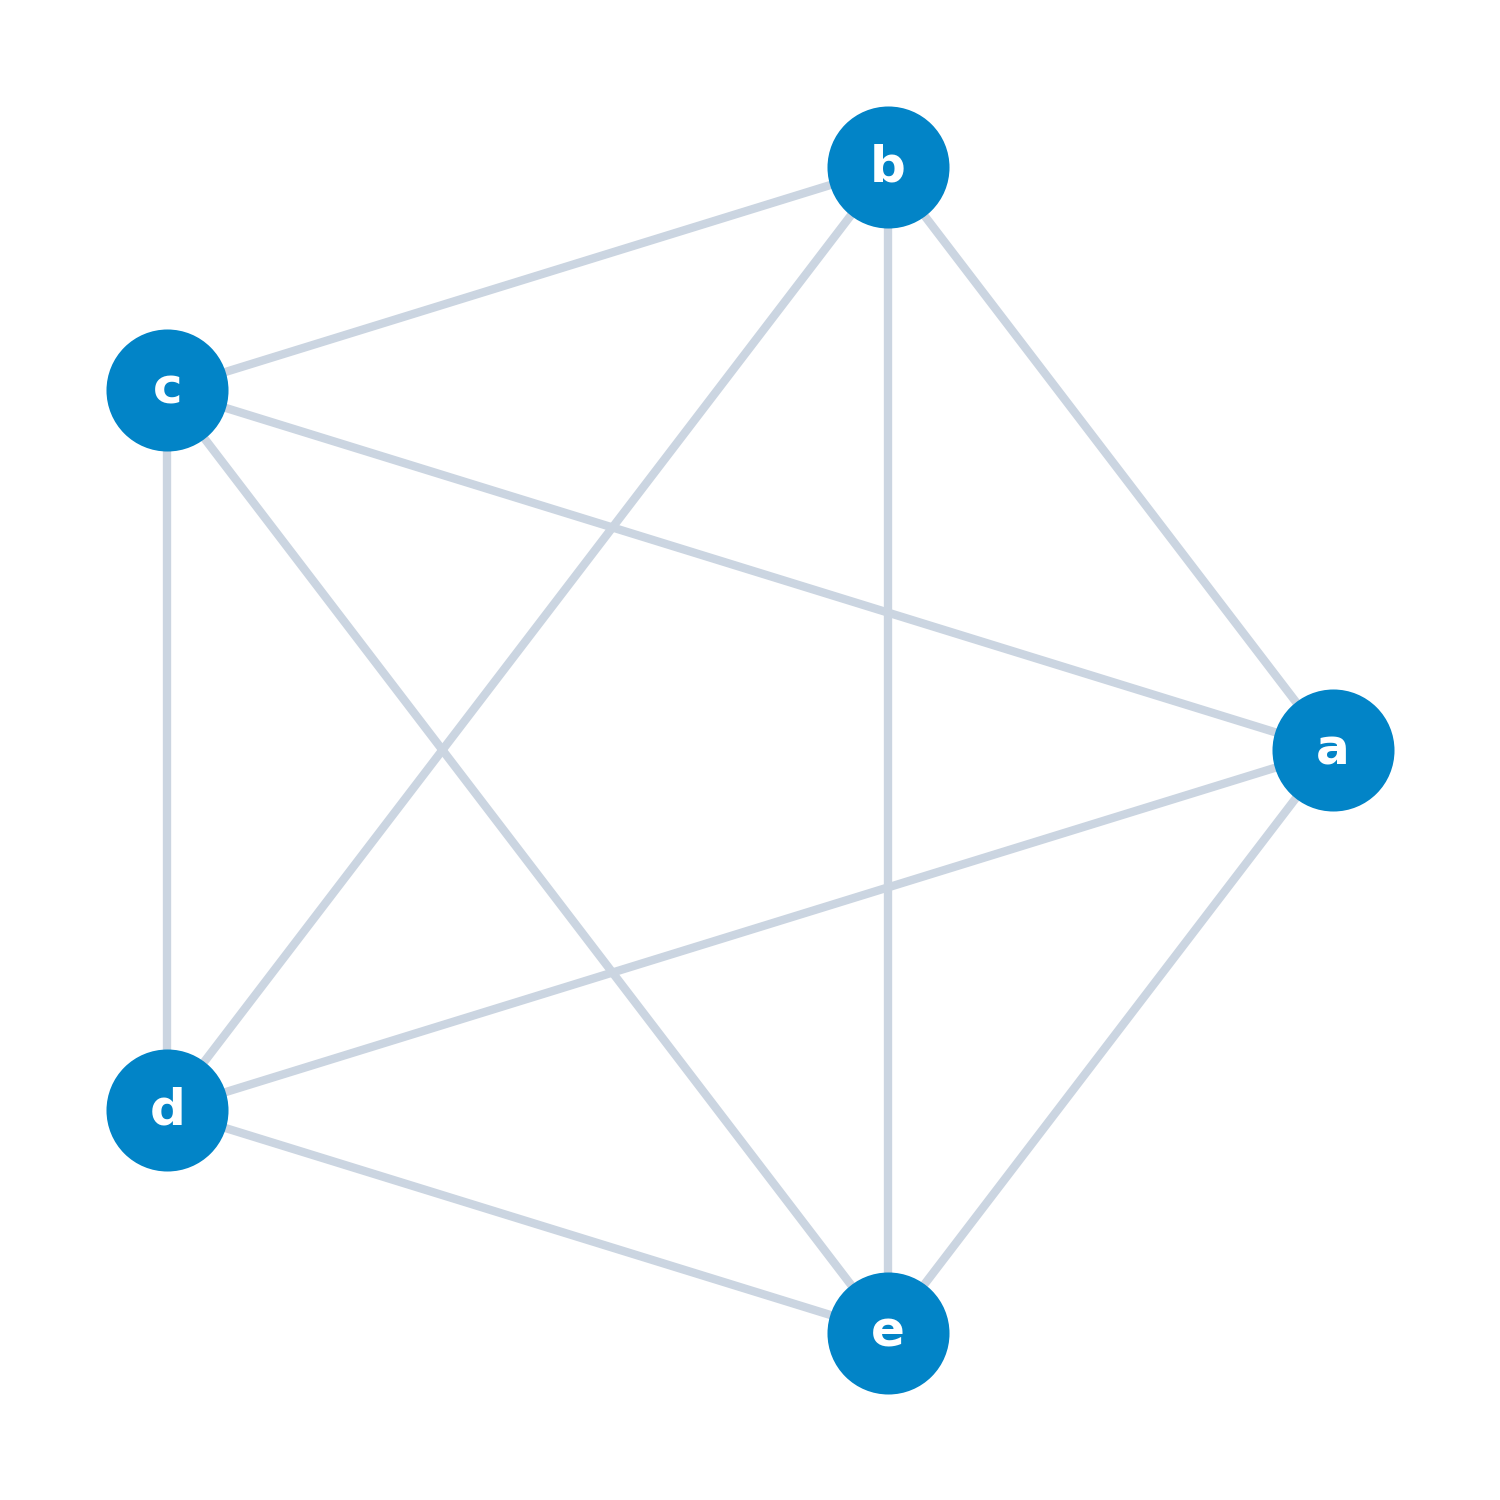
\includegraphics[width=0.4\linewidth,height=\textheight,keepaspectratio]{images/clan_k5_ejemplo.png}

}

\caption{\label{fig-clan-k5}Clan K5 simple completo sobre 5 vértices con
10 aristas}

\end{figure}%

En el estudio sintáctico de grandes redes, frecuentemente se requiere
extraer subestructuras más pequeñas limitando los elementos disponibles.
Para ello, se distingue rigurosamente entre la extracción guiada por
nodos (\textbf{subgrafo inducido}) y la extracción guiada por arcos
(\textbf{grafo parcial}).

\begin{tcolorbox}[enhanced jigsaw, toprule=.15mm, opacitybacktitle=0.6, coltitle=black, colbacktitle=quarto-callout-note-color!10!white, title=\textcolor{quarto-callout-note-color}{\faInfo}\hspace{0.5em}{Definición: Subgrafo generado (inducido) y grafo parcial}, arc=.35mm, rightrule=.15mm, toptitle=1mm, breakable, bottomtitle=1mm, titlerule=0mm, colback=white, opacityback=0, leftrule=.75mm, colframe=quarto-callout-note-color-frame, left=2mm, bottomrule=.15mm]

Dado un digrafo \(G = (V, U)\) (o grafo \(G = (V, E)\)):

\begin{itemize}
\item
  \textbf{Subgrafo Generado (Inducido)}: Dado un subconjunto de vértices
  \(A \subset V\), el subgrafo generado \(G_A = (A, U_A)\) conserva
  \textbf{únicamente} los nodos de \(A\) y las relaciones cuyos dos
  extremos pertenecen íntegramente a \(A\): \[
  U_A = \{u = (i, j) \in U : i, j \in A\}
  \]
\item
  \textbf{Grafo Parcial Generado}: Dado un subconjunto de arcos
  \(W \subset U\), el grafo parcial \(G(W) = (V, W)\) conserva el
  conjunto completo de \(n\) vértices originales de \(V\), pero
  restringe el conjunto de arcos a \(W\).
\end{itemize}

\end{tcolorbox}

Para comprender la diferencia intuitiva entre ambas operaciones,
considérese la red orientada original \(G = (V, U)\) de 5 nodos y 10
arcos representada en la Figura~\ref{fig-digrafo-base}.

\begin{figure}

\centering{

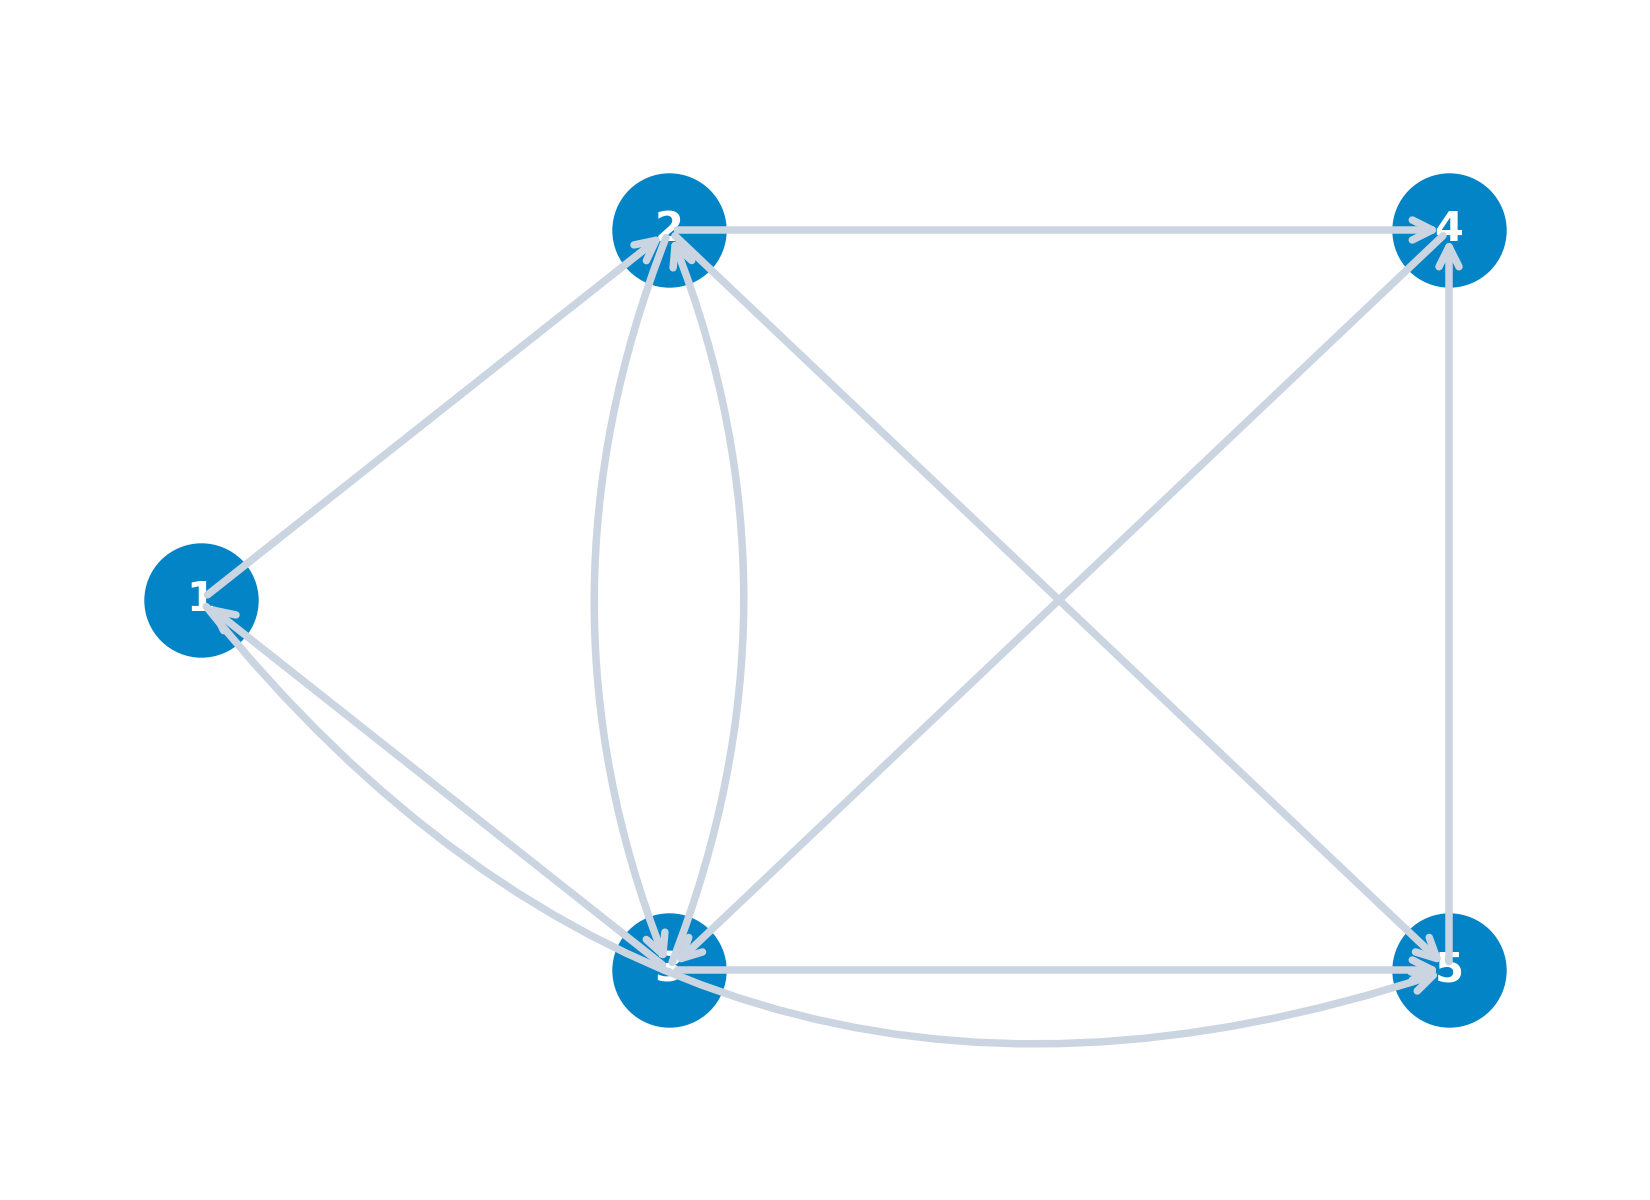
\includegraphics[width=0.5\linewidth,height=\textheight,keepaspectratio]{images/digrafo_base_original.png}

}

\caption{\label{fig-digrafo-base}Digrafo original de 5 nodos G=(V,U)}

\end{figure}%

Cuando se genera un subgrafo inducido seleccionando un subconjunto de
nodos \(A \subset V\), los vértices que no pertenecen a \(A\)
desaparecen por completo de la representación geométrica y algebraica.
Así, al elegir \(A = \{1, 2, 5\}\), la Figura~\ref{fig-subgrafo-a125}
muestra cómo la estructura resultante \(G_{\{1,2,5\}}\) conserva
únicamente los 3 nodos seleccionados y los 3 arcos que conectaban a
dichos nodos entre sí.

\begin{figure}

\centering{

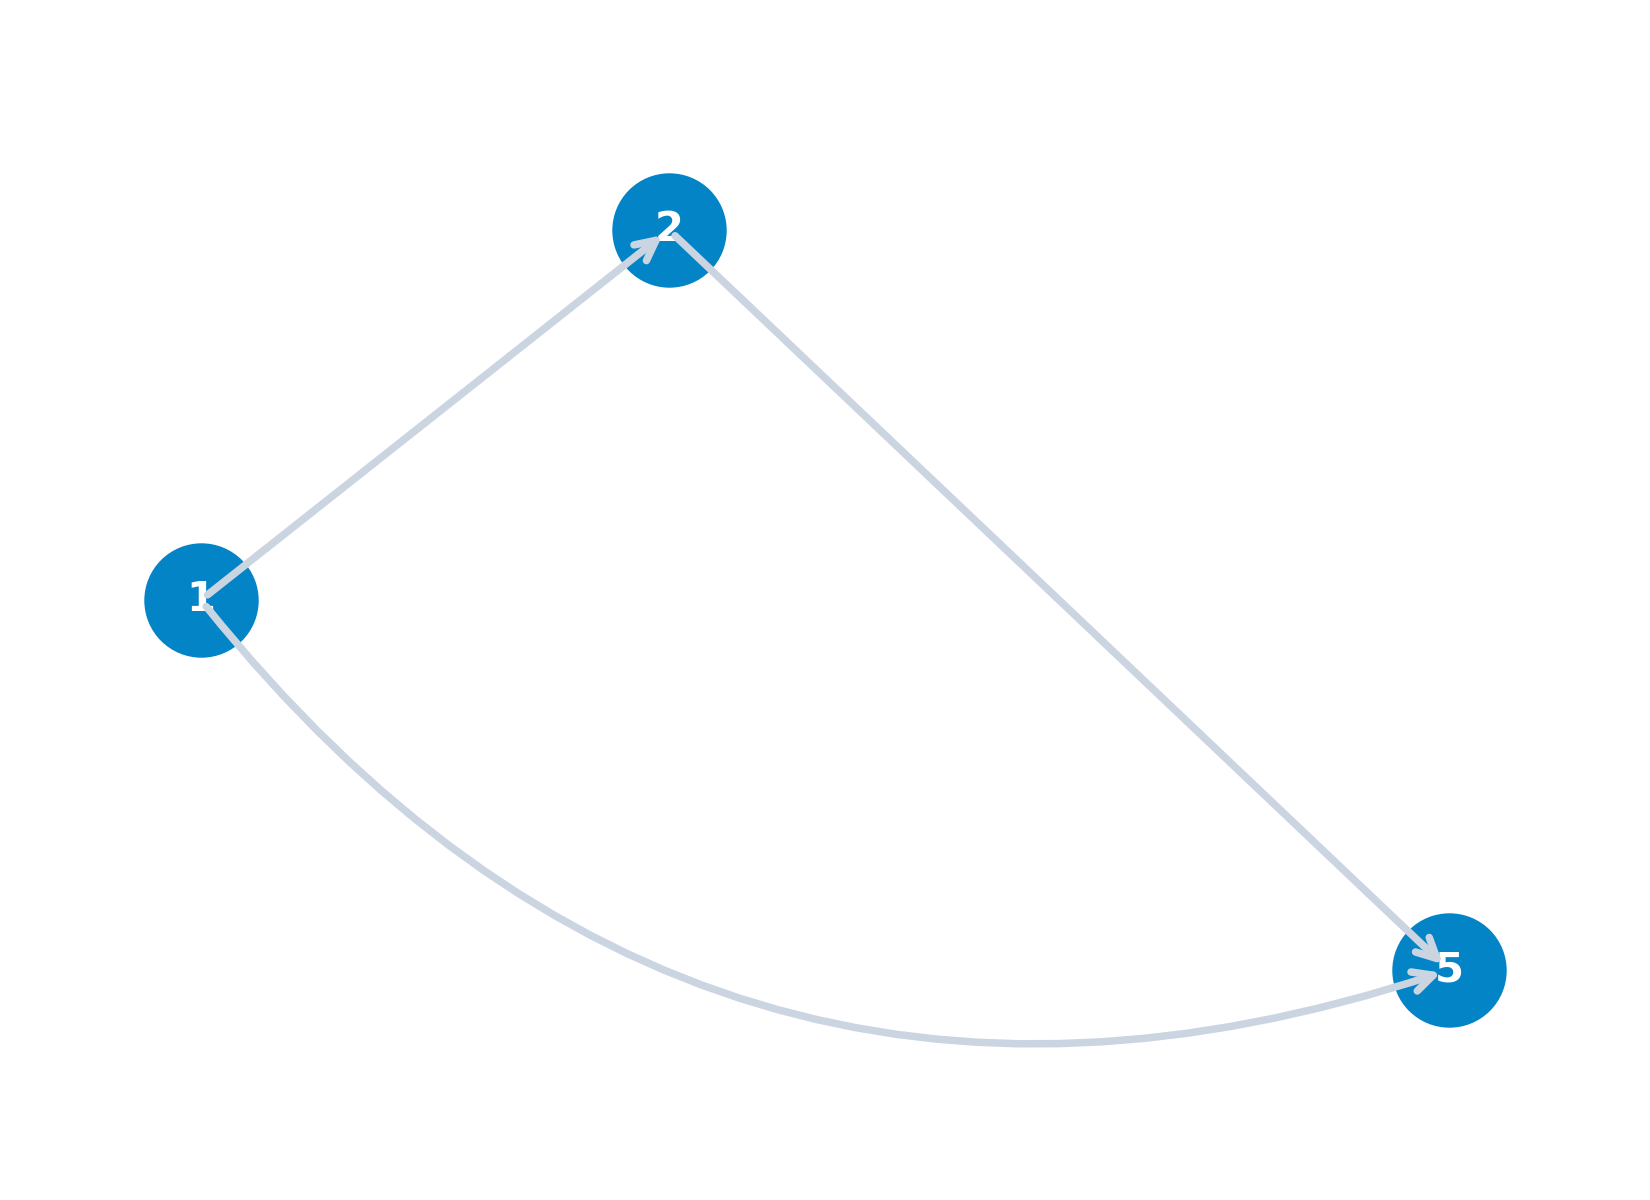
\includegraphics[width=0.5\linewidth,height=\textheight,keepaspectratio]{images/subgrafo_inducido_a125.png}

}

\caption{\label{fig-subgrafo-a125}Subgrafo inducido generado por el
subconjunto de nodos A=\{1,2,5\}}

\end{figure}%

Análogamente, al inducir la red sobre el subconjunto de nodos
\(A = \{1, 2, 3\}\), la Figura~\ref{fig-subgrafo-a123} refleja la
topología aislada \(G_{\{1,2,3\}}\), compuesta estrictamente por los 3
vértices de \(A\) y los 4 arcos internos que los unían en el grafo
original.

\begin{figure}

\centering{

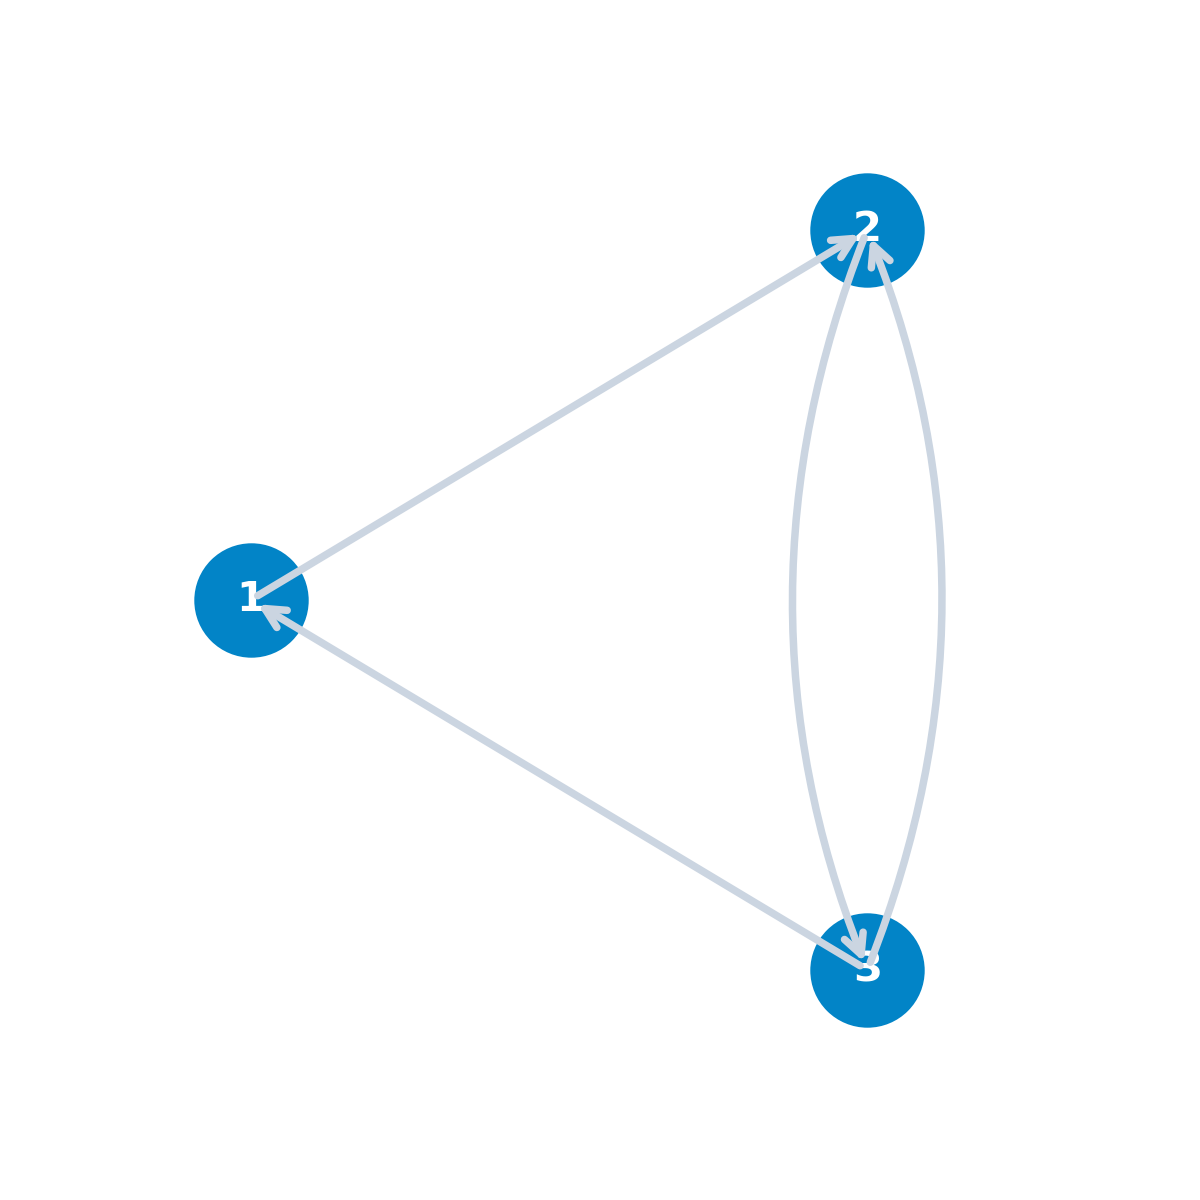
\includegraphics[width=0.4\linewidth,height=\textheight,keepaspectratio]{images/subgrafo_inducido_a123.png}

}

\caption{\label{fig-subgrafo-a123}Subgrafo inducido generado por el
subconjunto de nodos A=\{1,2,3\}}

\end{figure}%

Por el contrario, la extracción de un grafo parcial no altera el
conjunto de vértices de la red, manteniendo siempre presentes los
\(n=5\) nodos de \(V\). Si se selecciona el subconjunto de arcos
\(W = \{(1,2), (2,4), (5,4)\}\), la Figura~\ref{fig-grafo-parcial-w1}
muestra cómo el nodo 3 permanece en el grafo parcial \(G(W)\) en calidad
de nodo aislado sin grado de conexión (\(d(3)=0\)).

\begin{figure}

\centering{

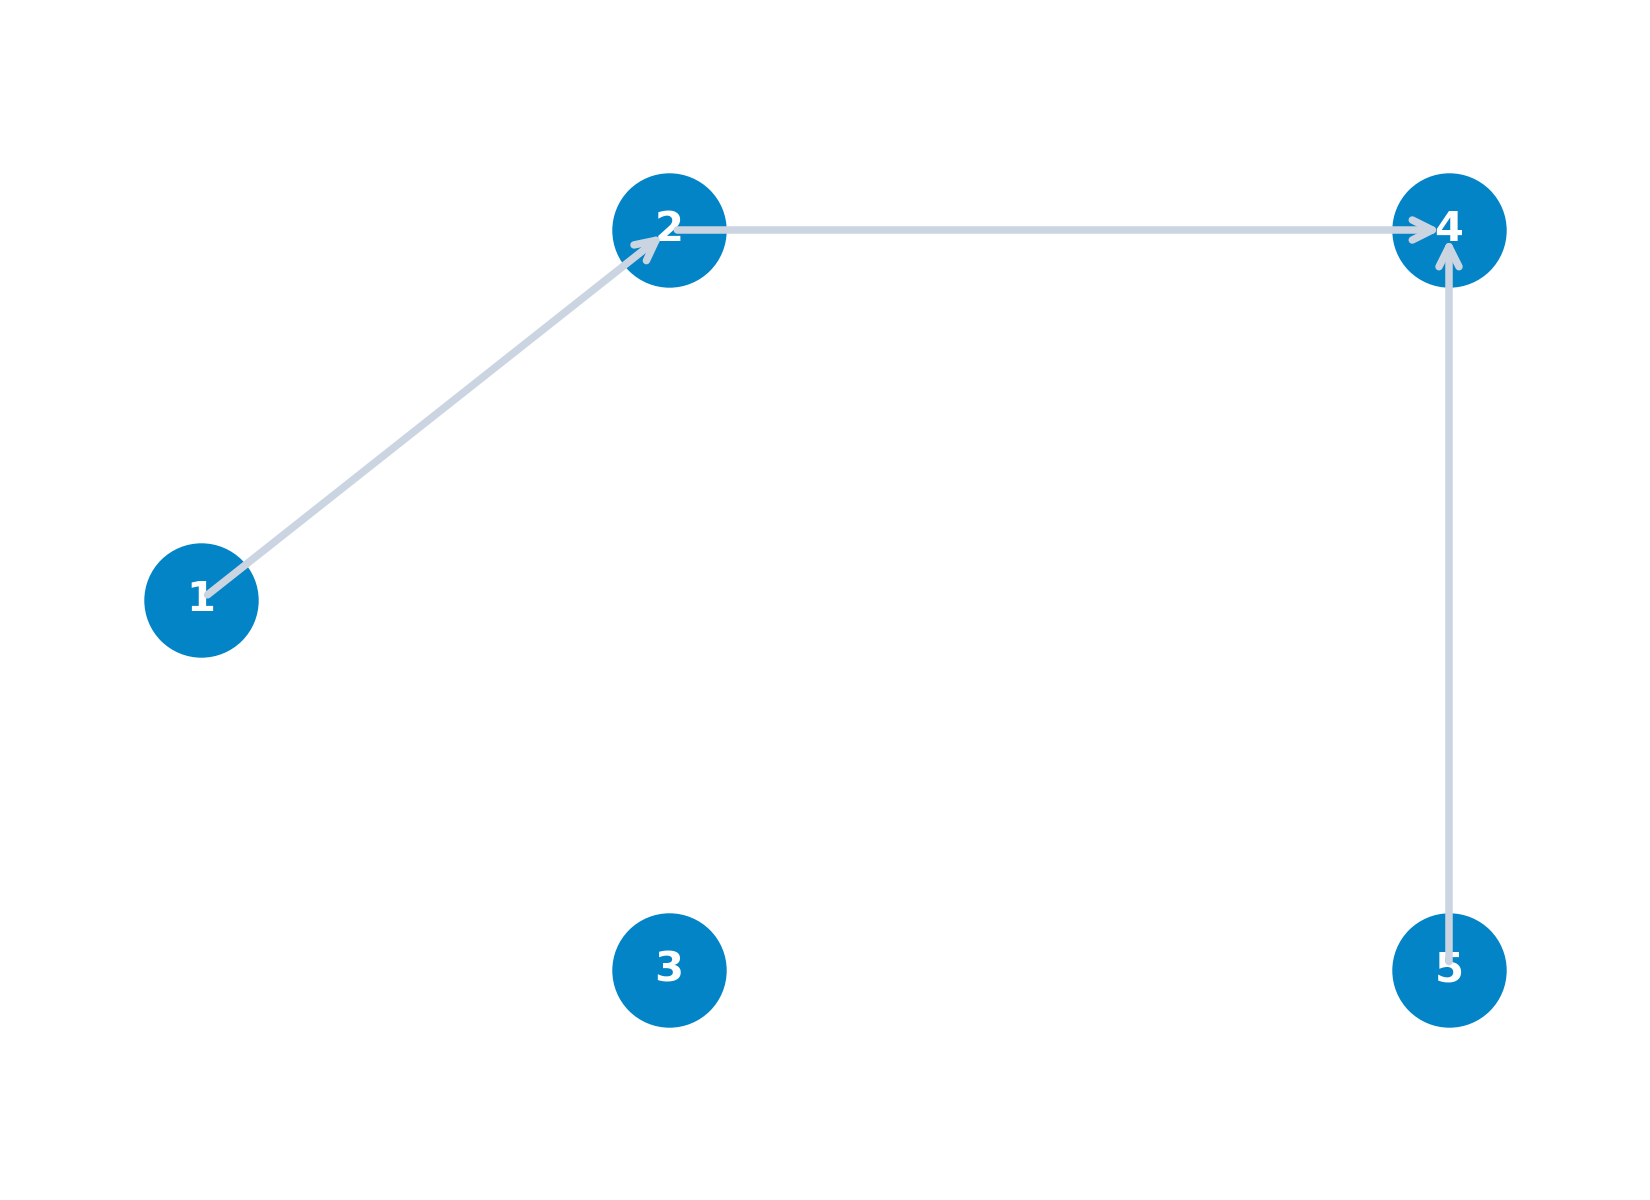
\includegraphics[width=0.5\linewidth,height=\textheight,keepaspectratio]{images/grafo_parcial_w1.png}

}

\caption{\label{fig-grafo-parcial-w1}Grafo parcial generado por el
subconjunto de arcos W = \{(1,2), (2,4), (5,4)\}}

\end{figure}%

Si en su lugar se elige el subconjunto de arcos
\(W = \{(1,2), (2,4), (2,5), (3,1)\}\), se obtiene el grafo parcial
representado en la Figura~\ref{fig-grafo-parcial-w2}, el cual preserva
los 5 vértices de \(V\) conectados mediante una topología arborescente
parcial.

\begin{figure}

\centering{

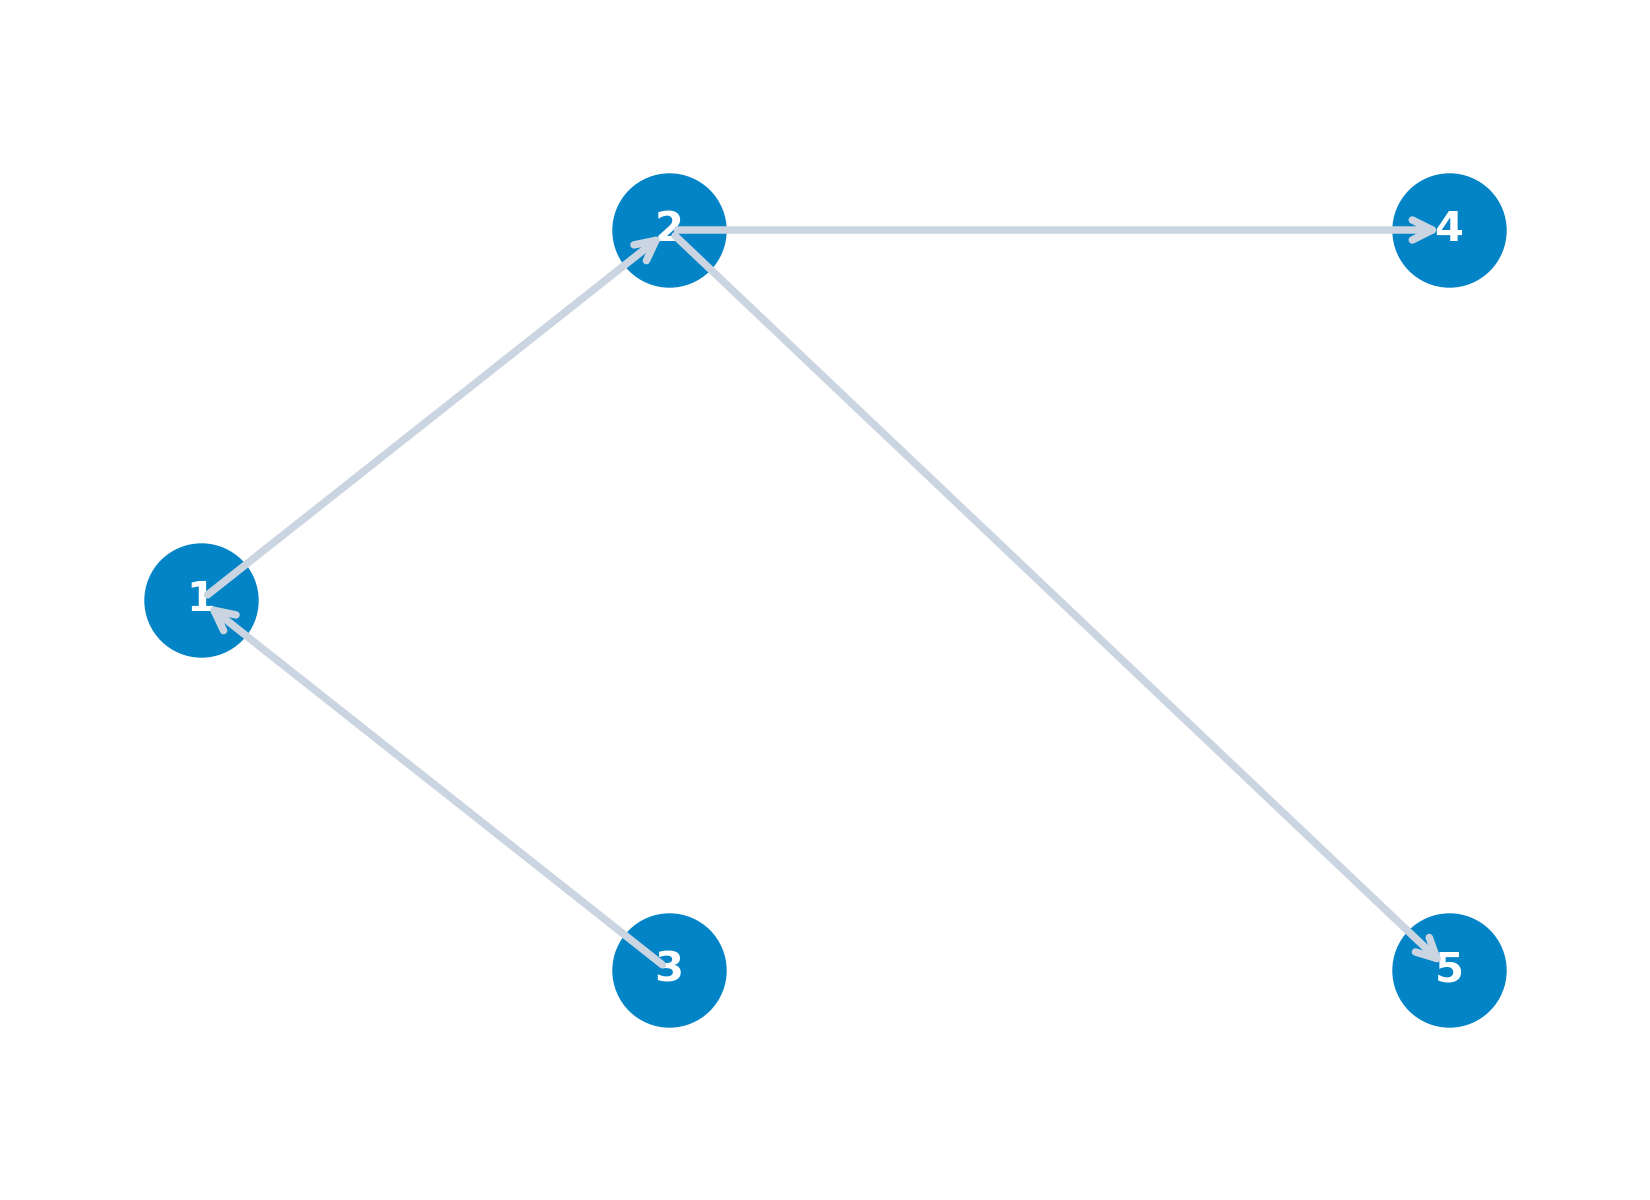
\includegraphics[width=0.5\linewidth,height=\textheight,keepaspectratio]{images/grafo_parcial_w2.png}

}

\caption{\label{fig-grafo-parcial-w2}Grafo parcial generado por el
subconjunto de arcos W = \{(1,2), (2,4), (2,5), (3,1)\}}

\end{figure}%

Finalmente, en la caracterización teórica de grafos simples resulta
relevante analizar las conexiones ``ausentes'' respecto a la red
completa mediante el concepto de grafo complementario.

\begin{tcolorbox}[enhanced jigsaw, toprule=.15mm, opacitybacktitle=0.6, coltitle=black, colbacktitle=quarto-callout-note-color!10!white, title=\textcolor{quarto-callout-note-color}{\faInfo}\hspace{0.5em}{Definición: Grafo complementario}, arc=.35mm, rightrule=.15mm, toptitle=1mm, breakable, bottomtitle=1mm, titlerule=0mm, colback=white, opacityback=0, leftrule=.75mm, colframe=quarto-callout-note-color-frame, left=2mm, bottomrule=.15mm]

Dado un grafo simple \(G = (V, E)\), el \textbf{grafo complementario}
\(\bar{G} = (V, \bar{E})\) mantiene el mismo conjunto de vértices \(V\)
y está formado exactamente por las aristas no presentes en \(E\): \[
\bar{G} = (V, \bar{E}) \quad \text{tal que} \quad \{i, j\} \in \bar{E} \iff \{i, j\} \notin E \quad (\forall i \neq j)
\]

\end{tcolorbox}

En la Figura~\ref{fig-grafo-complementario} se ilustra este proceso de
inversión topológica a partir de un grafo simple \(G\) de 5 vértices
\(V = \{a, b, c, d, e\}\) y 7 aristas. Puesto que en el grafo original
\(G\) el vértice \(b\) se encuentra conectado con todos los demás nodos,
en el grafo complementario \(\bar{G}\) las únicas 3 aristas resultantes
son \(\bar{E} = \{\{a,d\}, \{a,e\}, \{c,e\}\}\), pasando el vértice
\(b\) a convertirse en un nodo totalmente aislado.

\begin{figure}

\centering{

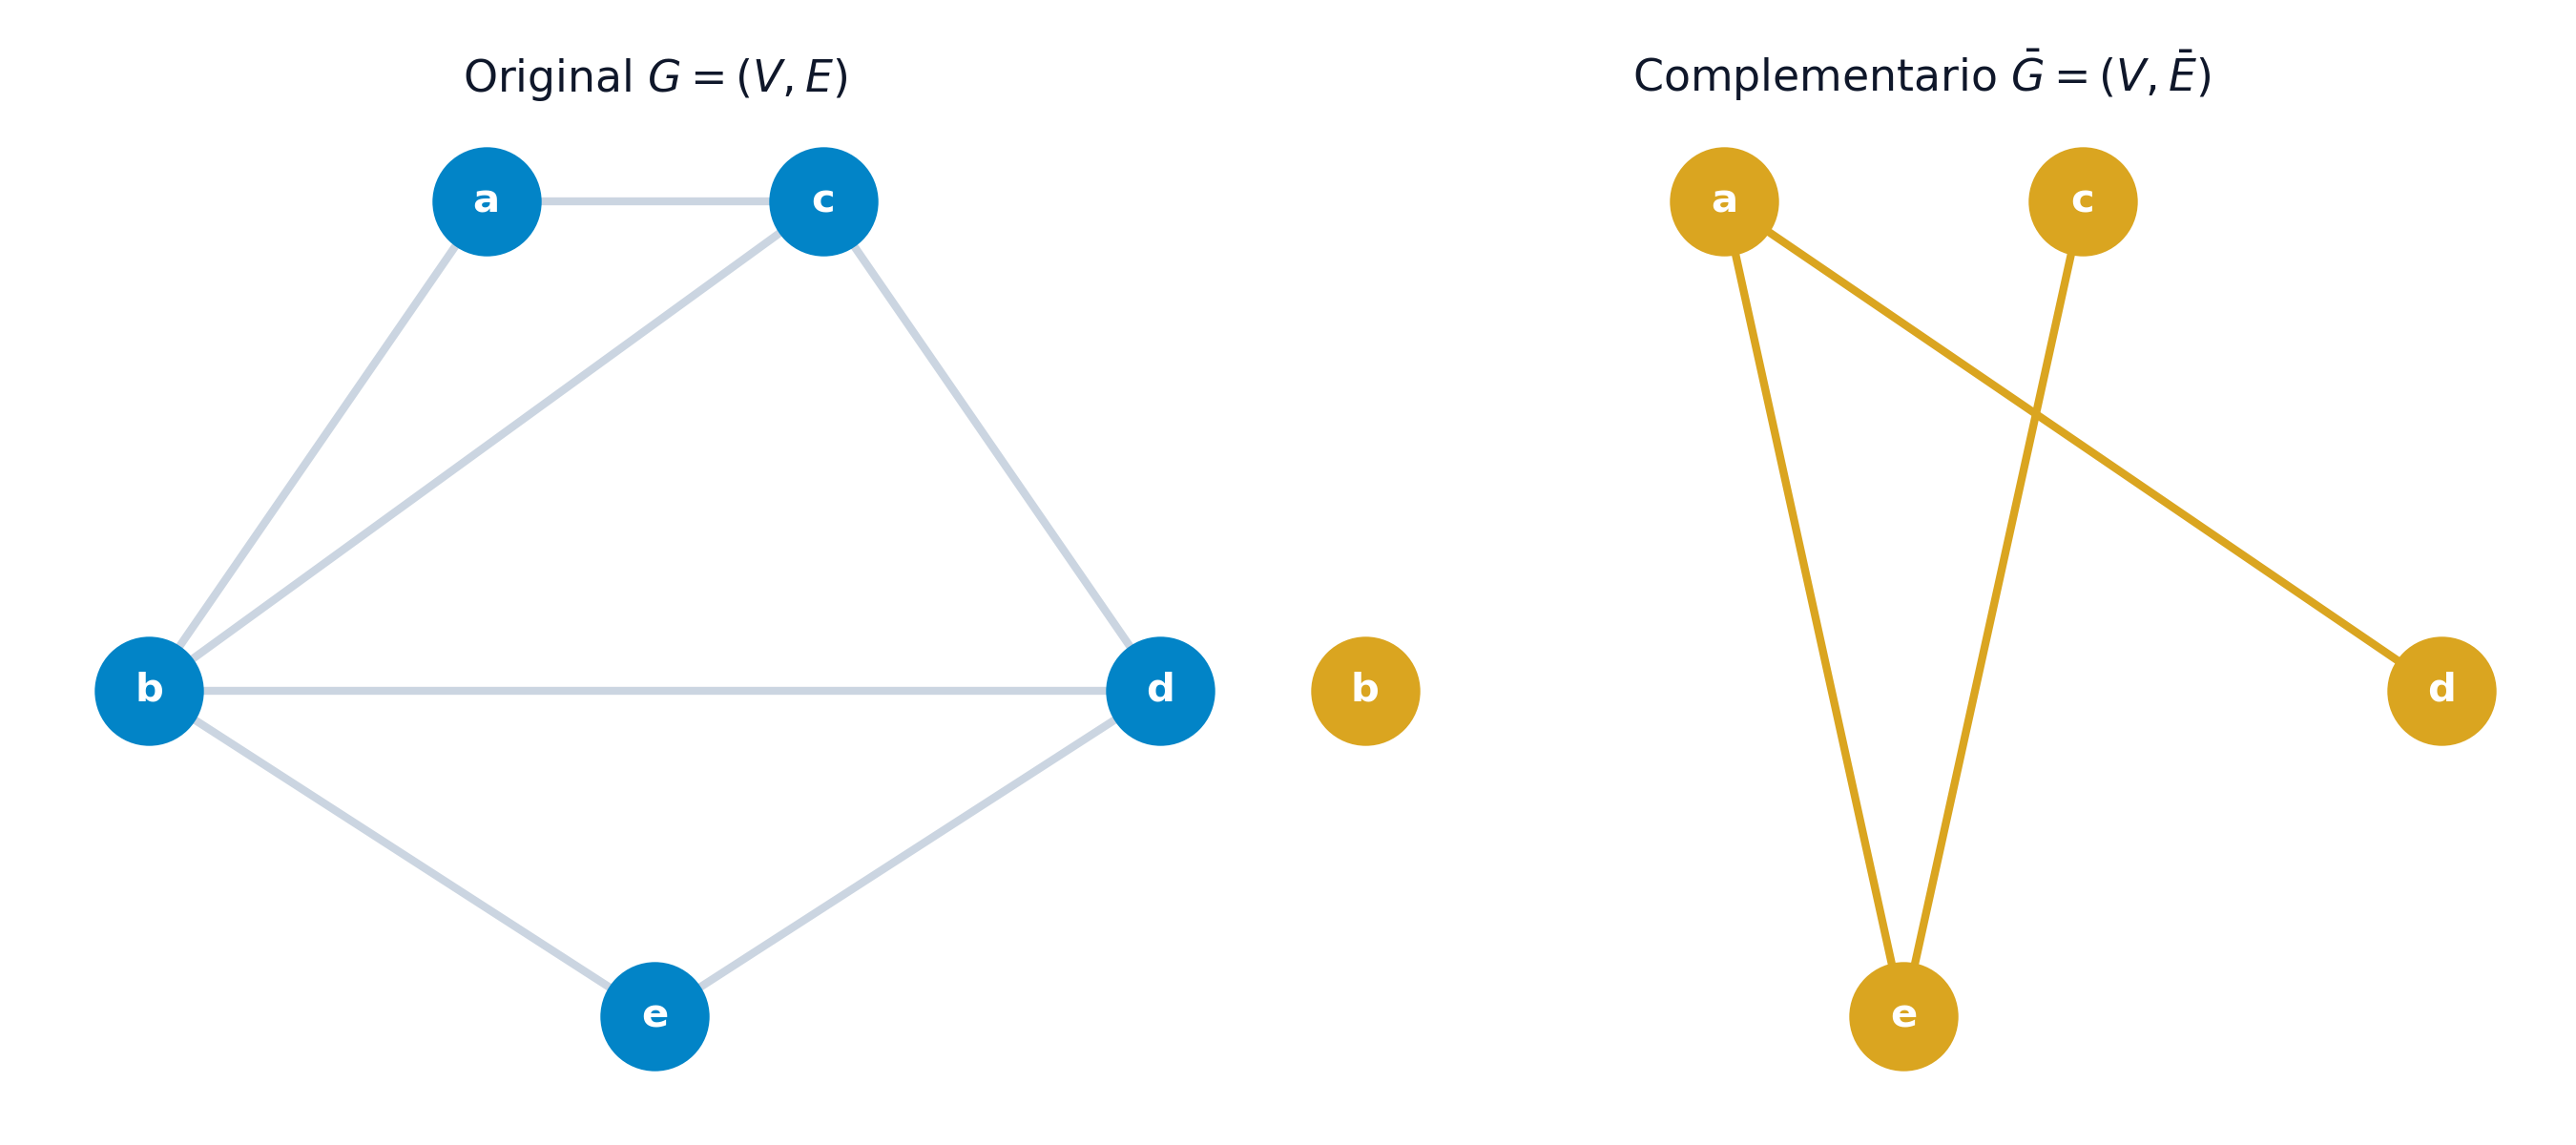
\includegraphics[width=0.75\linewidth,height=\textheight,keepaspectratio]{images/grafo_complementario.png}

}

\caption{\label{fig-grafo-complementario}Construcción del grafo
complementario para un grafo de 5 vértices}

\end{figure}%

\begin{center}\rule{0.5\linewidth}{0.5pt}\end{center}

\section{Recorridos y conectividad en
redes}\label{recorridos-y-conectividad-en-redes}

El análisis topológico de una red exige estudiar cómo la información, el
tráfico o los flujos se desplazan a través de sus vértices y conexiones.
Para ello, es preciso formalizar las secuencias de trayectorias (cadenas
y caminos), cuantificar sus métricas de alcance (distancia y diámetro) y
evaluar la capacidad global de comunicación e integridad del grafo
mediante el concepto de conectividad.

\subsection{Cadenas y caminos}\label{cadenas-y-caminos}

En la teoría de redes orientadas (Ahuja, Magnanti, y Orlin 1993), el
estudio del movimiento a través de los arcos requiere distinguir entre
recorridos que respetan la orientación de las flechas (caminos) y
recorridos que transitan los arcos sin importar su dirección (cadenas).

\begin{tcolorbox}[enhanced jigsaw, toprule=.15mm, opacitybacktitle=0.6, coltitle=black, colbacktitle=quarto-callout-note-color!10!white, title=\textcolor{quarto-callout-note-color}{\faInfo}\hspace{0.5em}{Definición: Cadena, camino, elementalidad y simplicidad}, arc=.35mm, rightrule=.15mm, toptitle=1mm, breakable, bottomtitle=1mm, titlerule=0mm, colback=white, opacityback=0, leftrule=.75mm, colframe=quarto-callout-note-color-frame, left=2mm, bottomrule=.15mm]

Dado un digrafo \(G = (V, U)\):

\begin{itemize}
\item
  \textbf{Cadena}: Secuencia de arcos adyacentes
  \(\mu = (u_1, u_2, \dots, u_q)\) de longitud \(q \ge 1\) entre los
  nodos extremos \(i\) y \(j\) (\(\mu[i, j]\)) en la que los arcos
  pueden recorrerse a favor o en contra de su orientación original.
\item
  \textbf{Camino}: Cadena orientada en la que todos los arcos se
  transitan estrictamente a favor de su sentido; es decir, el nodo final
  de \(u_k\) coincide con el nodo inicial de \(u_{k+1}\) para todo
  \(k = 1, \dots, q-1\).
\item
  \textbf{Elemental}: Una cadena o camino es \textbf{elemental} si no
  repite ningún vértice en su recorrido.
\item
  \textbf{Simple}: Una cadena o camino es \textbf{simple} si no repite
  ningún arco en su recorrido.
\end{itemize}

\end{tcolorbox}

Para analizar las propiedades de simplicidad y elementalidad sobre redes
orientadas, considérese la red de 6 aeropuertos internacionales
\(V = \{m, l, p, f, s, t\}\) (Madrid, Londres, París, Frankfurt,
Singapur y Tokio).

Un primer caso lo constituye la cadena
\(\mu^1[m, p] = \{(m, l); (l, f); (p, f)\}\), de longitud \(q=3\). Este
recorrido resulta ser \textbf{elemental y simple}, ya que transita por
los 4 vértices \(\{m, l, f, p\}\) sin repetir ninguno y recorre 3 arcos
distintos. Puesto que el arco \((p, f)\) se atraviesa en sentido inverso
(desde \(f\) hasta \(p\)), se trata de una cadena y no de un camino. La
Figura~\ref{fig-cadena-mu1} ilustra este trayecto en la red.

\begin{figure}

\centering{

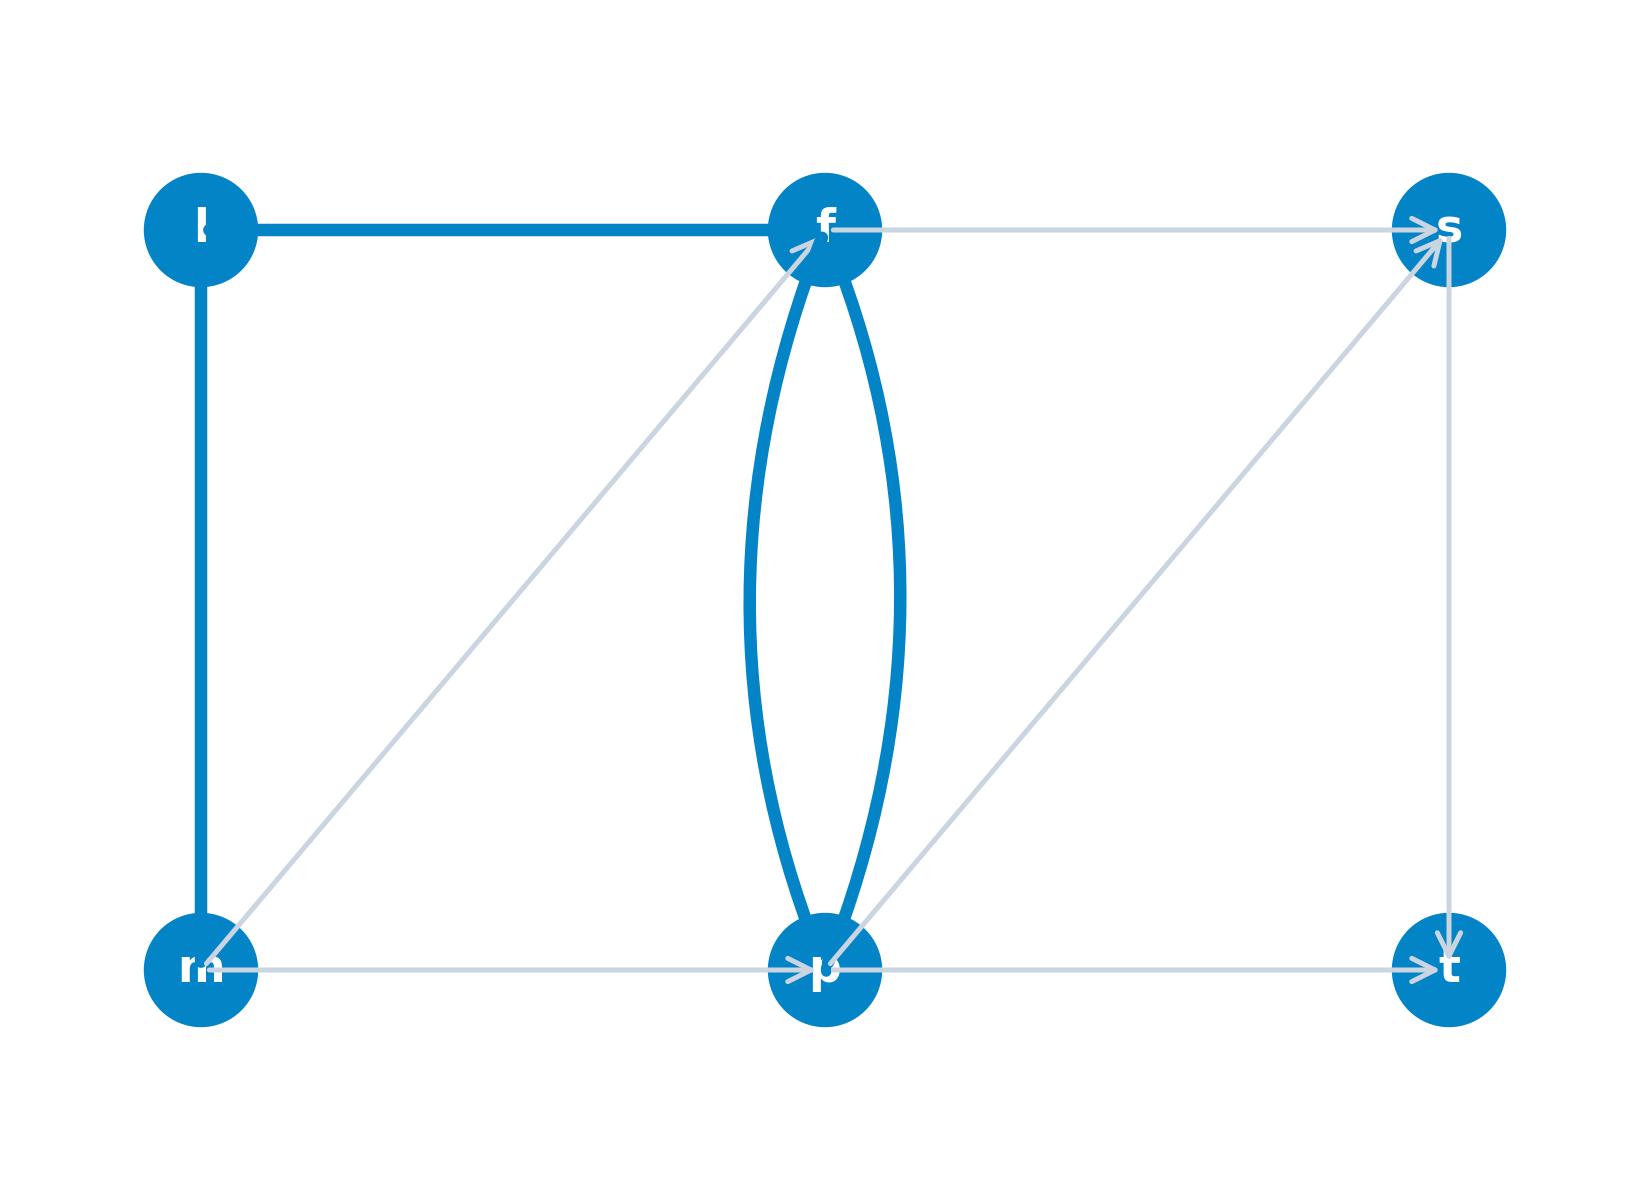
\includegraphics[width=0.55\linewidth,height=\textheight,keepaspectratio]{images/cadena_ejemplo_mu1.png}

}

\caption{\label{fig-cadena-mu1}Cadena mu1{[}m, p{]} elemental y simple
con el arco (p, f) recorrido en sentido inverso}

\end{figure}%

Cuando la trayectoria respeta la dirección de todas las flechas y no
repite elementos, se genera un camino perfecto. La secuencia
\(\mu^2[p, t] = \{(p, f); (f, s); (s, t)\}\) entre París (\(p\)) y Tokio
(\(t\)) constituye un \textbf{camino elemental y simple} de longitud
\(q=3\). Como se observa en la Figura~\ref{fig-cadena-mu2}, los tres
arcos avanzan fluidamente en el sentido marcado por la red.

\begin{figure}

\centering{

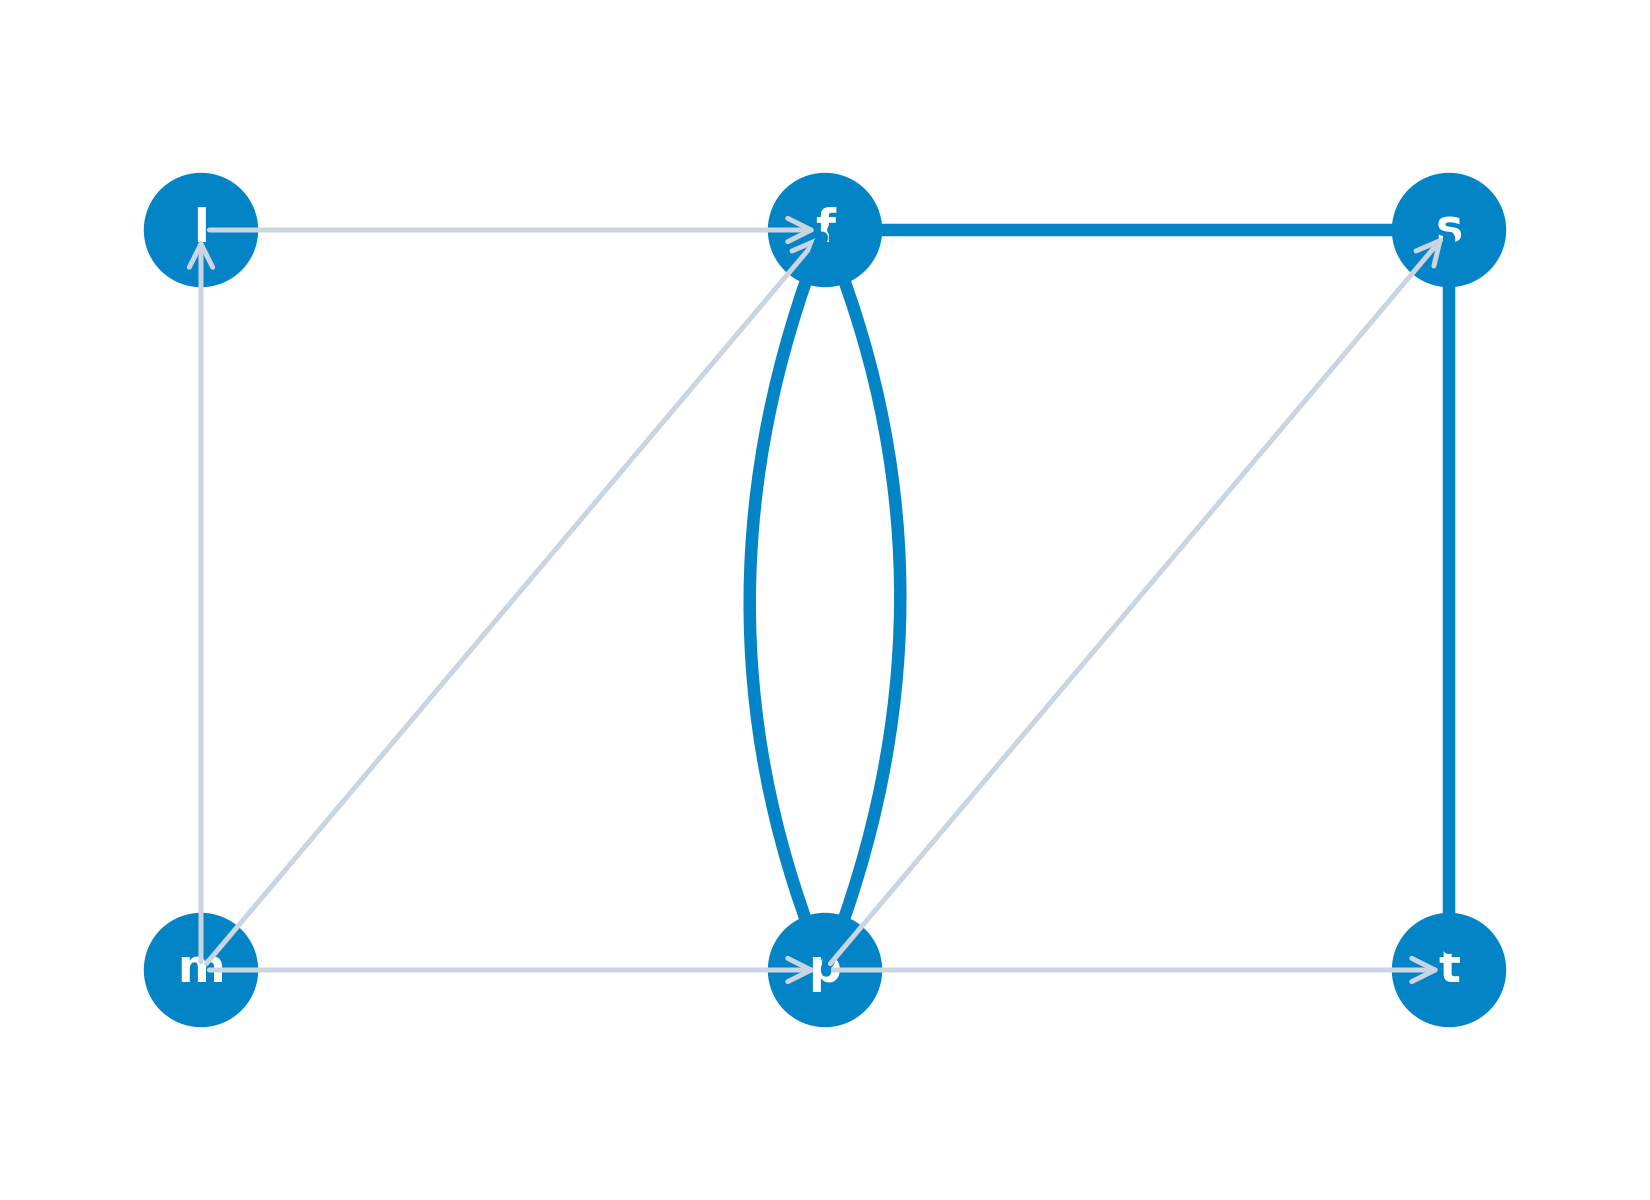
\includegraphics[width=0.55\linewidth,height=\textheight,keepaspectratio]{images/cadena_ejemplo_mu2.png}

}

\caption{\label{fig-cadena-mu2}Camino mu2{[}p, t{]} elemental y simple
con todos los arcos en sentido directo}

\end{figure}%

Es posible que un recorrido no repita ningún arco pero sí vuelva a pasar
por un vértice previamente visitado. La cadena
\(\mu^3[m, p] = \{(m, p); (p, f); (f, s); (p, s); (p, t)\}\), de
longitud \(q=5\), es \textbf{no elemental y sí simple}. Como refleja la
Figura~\ref{fig-cadena-mu3}, la trayectoria visita dos veces el nodo
\(p\) (\(m \to p \to f \to s \to p \to t\)), pero mantiene la
simplicidad al no duplicar ninguno de sus 5 arcos.

\begin{figure}

\centering{

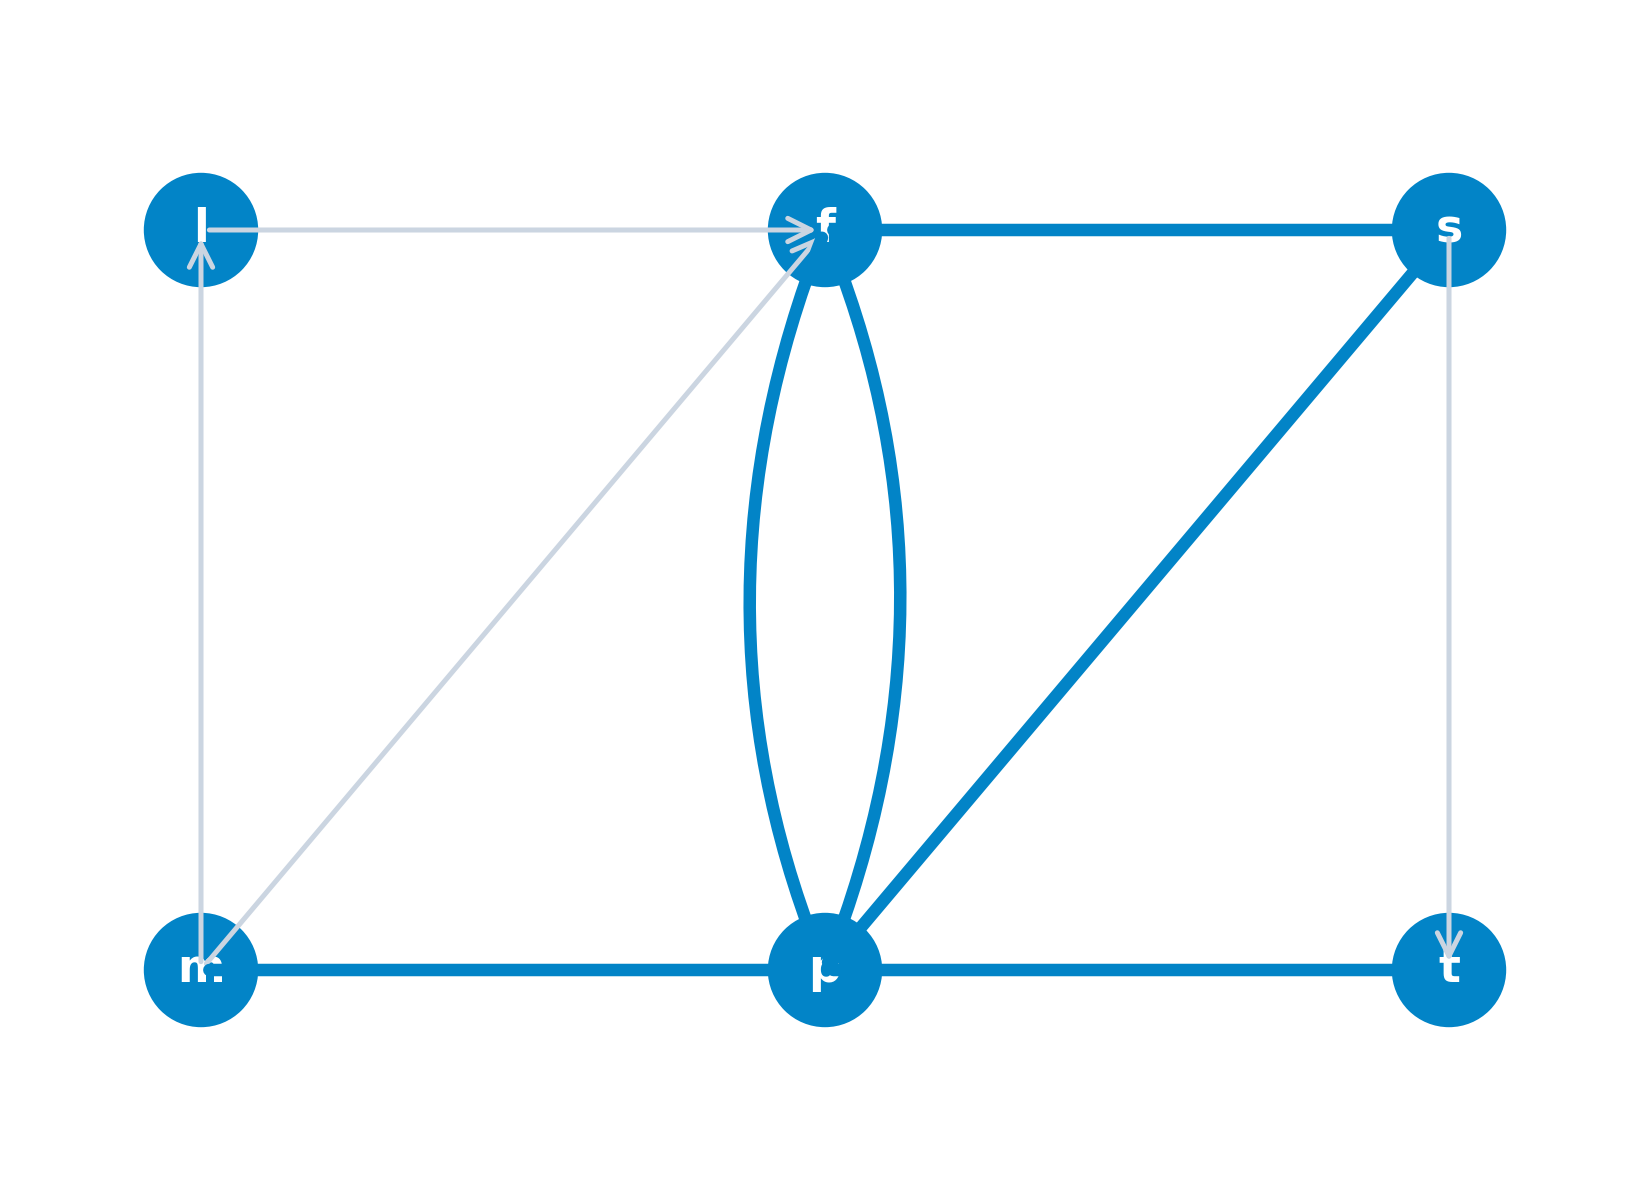
\includegraphics[width=0.55\linewidth,height=\textheight,keepaspectratio]{images/cadena_ejemplo_mu3.png}

}

\caption{\label{fig-cadena-mu3}Cadena mu3{[}m, p{]} no elemental y sí
simple con visita duplicada al nodo p}

\end{figure}%

Por último, cuando un recorrido duplica tanto nodos como conexiones,
pierde ambas propiedades. La cadena
\(\mu^4 = \{(l, f); (f, s); (p, s); (p, f); (f, s); (s, t)\}\), de
longitud \(q=6\), es \textbf{ni elemental ni simple}. Como muestra la
Figura~\ref{fig-cadena-mu4}, el arco \((f, s)\) se transita dos veces en
instantes distintos del recorrido.

\begin{figure}

\centering{

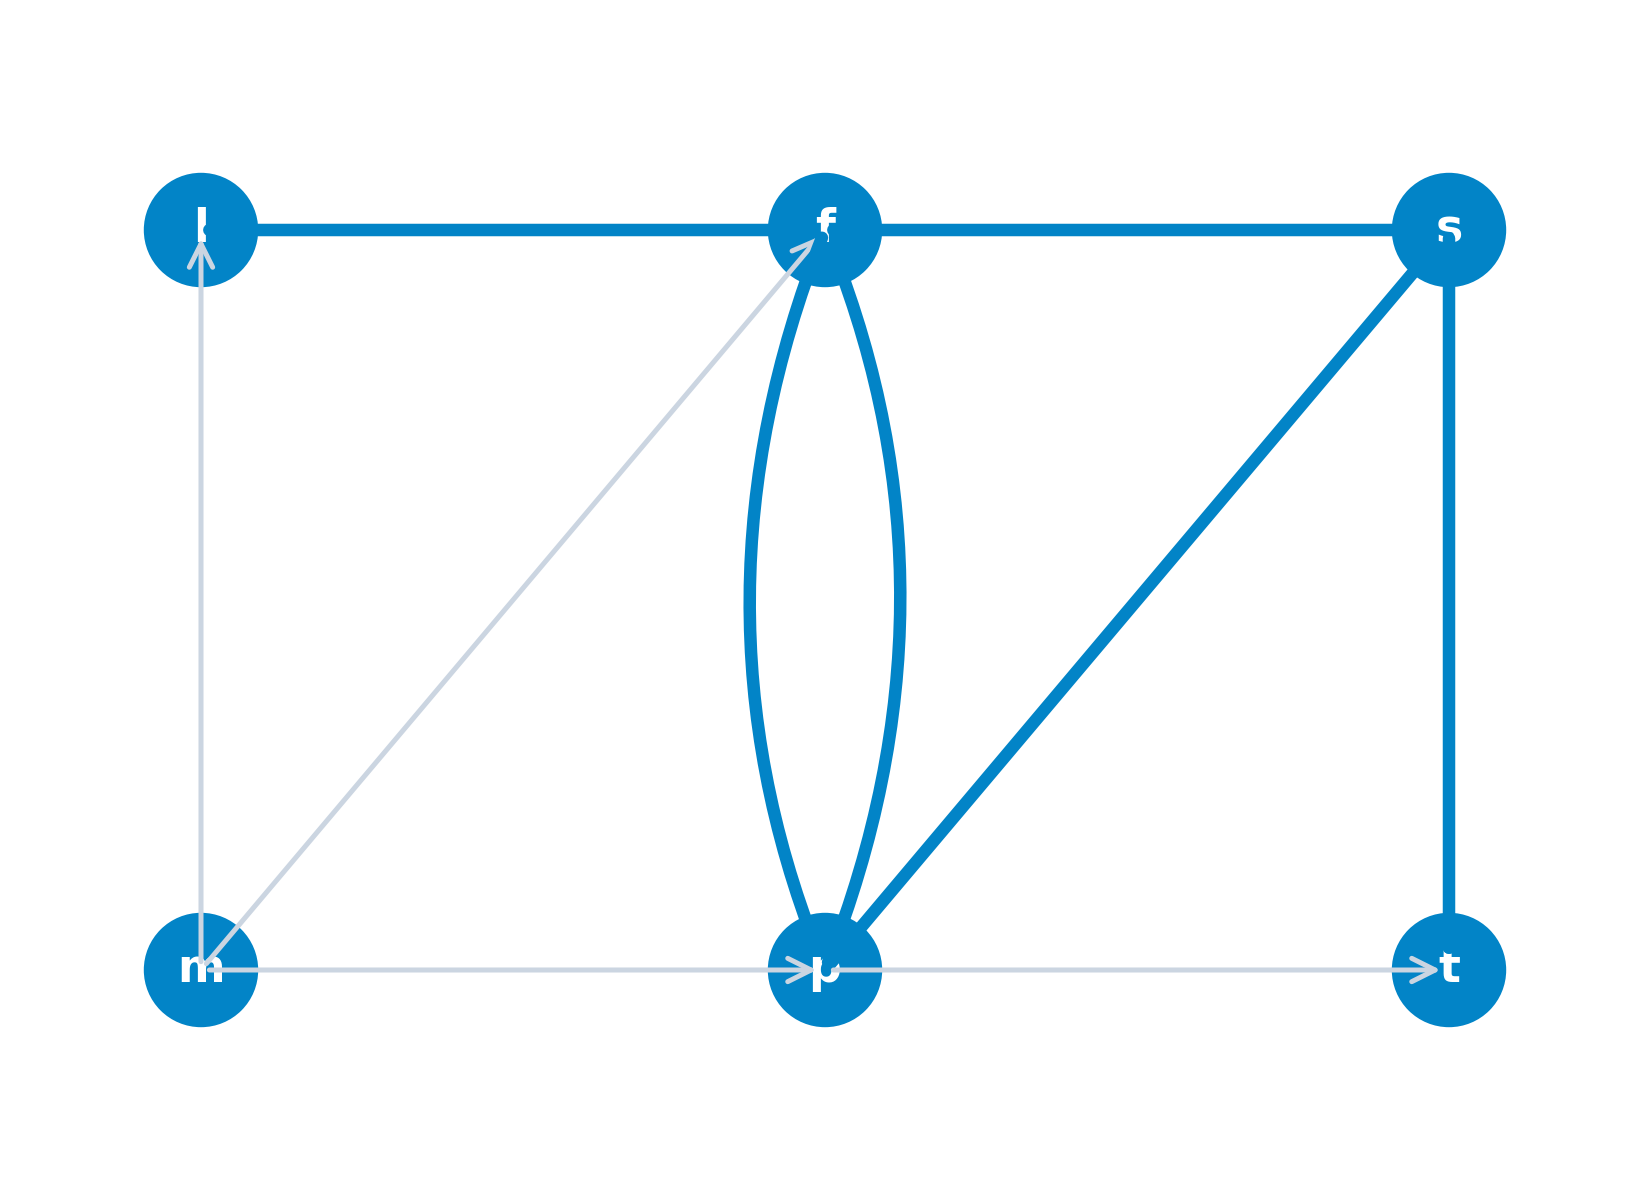
\includegraphics[width=0.55\linewidth,height=\textheight,keepaspectratio]{images/cadena_ejemplo_mu4.png}

}

\caption{\label{fig-cadena-mu4}Cadena mu4 ni elemental ni simple con
repetición del arco (f, s)}

\end{figure}%

\begin{tcolorbox}[enhanced jigsaw, toprule=.15mm, opacitybacktitle=0.6, coltitle=black, colbacktitle=quarto-callout-tip-color!10!white, title=\textcolor{quarto-callout-tip-color}{\faLightbulb}\hspace{0.5em}{Ejemplo: Clasificación de cadenas en grafos (elementalidad y
simplicidad)}, arc=.35mm, rightrule=.15mm, toptitle=1mm, breakable, bottomtitle=1mm, titlerule=0mm, colback=white, opacityback=0, leftrule=.75mm, colframe=quarto-callout-tip-color-frame, left=2mm, bottomrule=.15mm]

Considérese un grafo no dirigido sobre 5 vértices
\(V = \{1, 2, 3, 4, 5\}\) y el análisis de las propiedades de
elementalidad y simplicidad para tres cadenas distintas:

\begin{enumerate}
\def\labelenumi{\arabic{enumi}.}
\item
  \textbf{Cadena \(\mu_1 = \{\{1,2\}, \{2,3\}, \{3,4\}, \{4,5\}\}\)}:
  Visita 5 vértices distintos sin duplicar ninguno (\(\{1,2,3,4,5\}\)) y
  transita por 4 aristas distintas. Por consiguiente, resulta ser una
  cadena \textbf{elemental y simple}.
\item
  \textbf{Cadena
  \(\mu_2 = \{\{1,2\}, \{2,3\}, \{3,4\}, \{4,2\}, \{2,5\}\}\)}: Recorre
  5 aristas distintas sin repetir ninguna (conserva la simplicidad),
  pero el nodo 2 es visitado dos veces durante la secuencia
  (\(1 \to 2 \to 3 \to 4 \to 2 \to 5\)). Por tanto, es una cadena
  \textbf{simple pero no elemental}.
\item
  \textbf{Cadena
  \(\mu_3 = \{\{1,2\}, \{2,4\}, \{4,3\}, \{3,2\}, \{2,1\}\}\)}: Duplica
  vértices (visita 2 múltiples veces) y además transita por la arista
  \(\{1,2\}\) dos veces (en ida y vuelta). Por tanto, es una cadena
  \textbf{ni elemental ni simple}.
\end{enumerate}

\begin{figure}[H]

\centering{

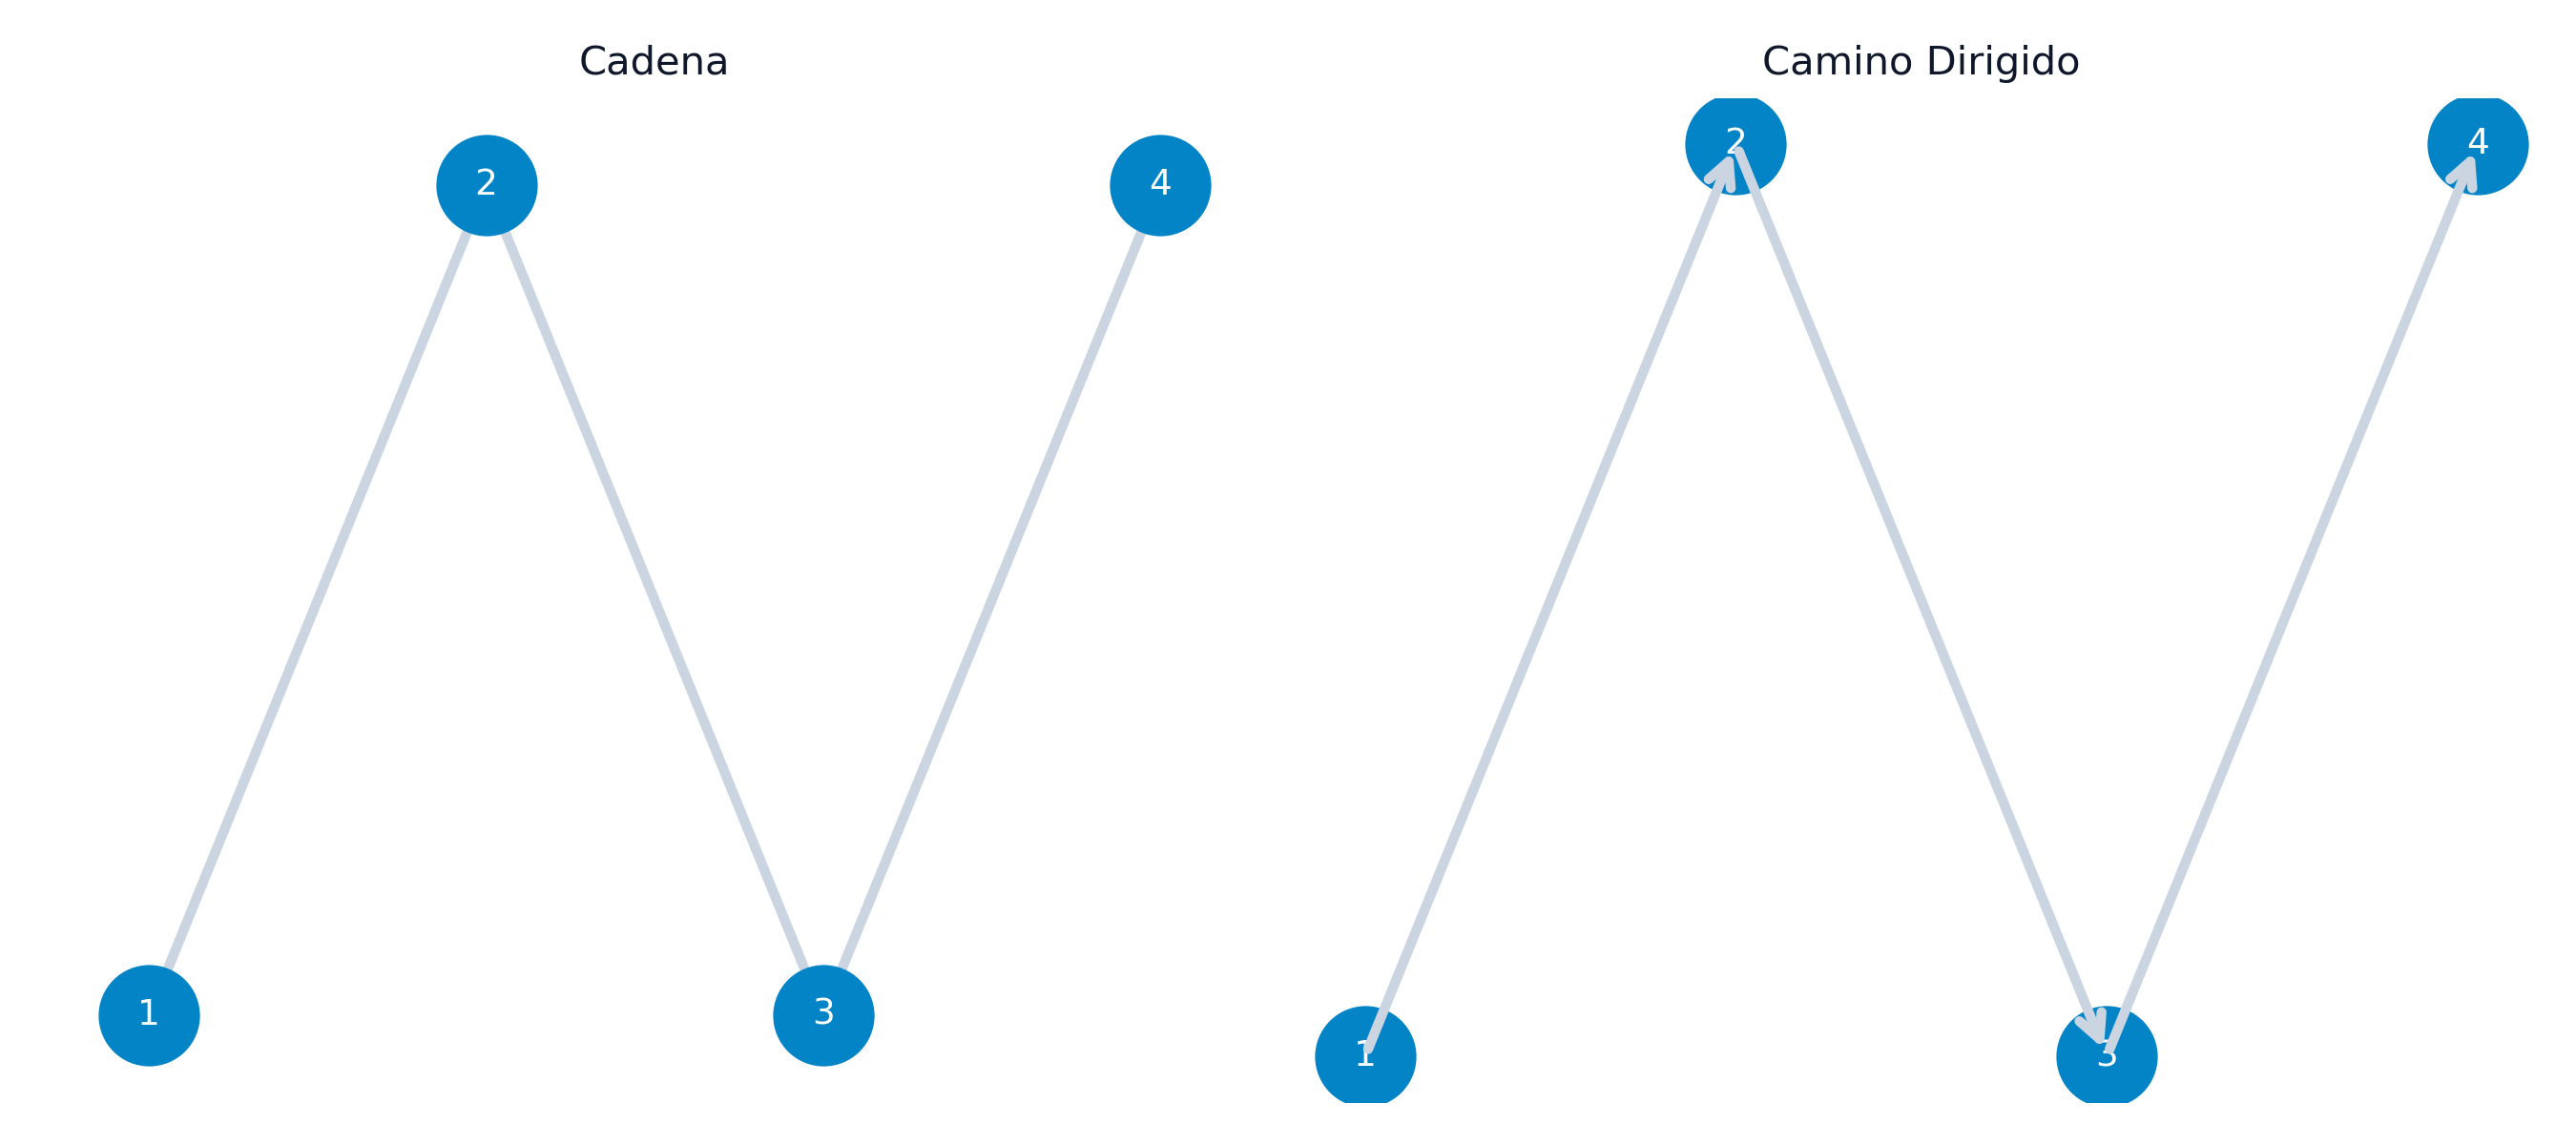
\includegraphics[width=0.75\linewidth,height=\textheight,keepaspectratio]{images/cadenas_caminos_diferencia.png}

}

\caption{\label{fig-cadenas-clasificacion-animado}Clasificación de
cadenas según su elementalidad y simplicidad}

\end{figure}%

\end{tcolorbox}

\begin{tcolorbox}[enhanced jigsaw, toprule=.15mm, opacitybacktitle=0.6, coltitle=black, colbacktitle=quarto-callout-tip-color!10!white, title=\textcolor{quarto-callout-tip-color}{\faLightbulb}\hspace{0.5em}{Ejemplo: Clasificación de caminos dirigidos (elementalidad y
simplicidad)}, arc=.35mm, rightrule=.15mm, toptitle=1mm, breakable, bottomtitle=1mm, titlerule=0mm, colback=white, opacityback=0, leftrule=.75mm, colframe=quarto-callout-tip-color-frame, left=2mm, bottomrule=.15mm]

Considérese una red dirigida sobre 7 vértices
\(V = \{a, b, c, d, e, f, g\}\) y el análisis de las propiedades de
elementalidad y simplicidad para tres caminos orientados:

\begin{enumerate}
\def\labelenumi{\arabic{enumi}.}
\item
  \textbf{Camino \(P_1 = ((a,b), (b,c), (c,e), (e,f))\)}: Transita en
  sentido directo por 5 vértices distintos
  (\(a \to b \to c \to e \to f\)) y 4 arcos distintos. Por tanto, es un
  \textbf{camino elemental y simple}.
\item
  \textbf{Camino \(P_2 = ((c,g), (g,f), (f,b), (b,c), (c,e))\)}: Recorre
  5 arcos distintos sin duplicar ninguno (conserva la simplicidad), pero
  el nodo \(c\) es visitado dos veces durante el recorrido
  (\(c \to g \to f \to b \to c \to e\)). Por tanto, es un \textbf{camino
  simple pero no elemental}.
\item
  \textbf{Camino \(P_3 = ((c,e), (e,f), (f,b), (b,c), (c,e), (e,g))\)}:
  Repite vértices (\(c\) y \(e\)) y además recorre el arco directed
  \((c,e)\) dos veces. Por tanto, es un \textbf{camino ni elemental ni
  simple}.
\end{enumerate}

\begin{figure}[H]

\centering{

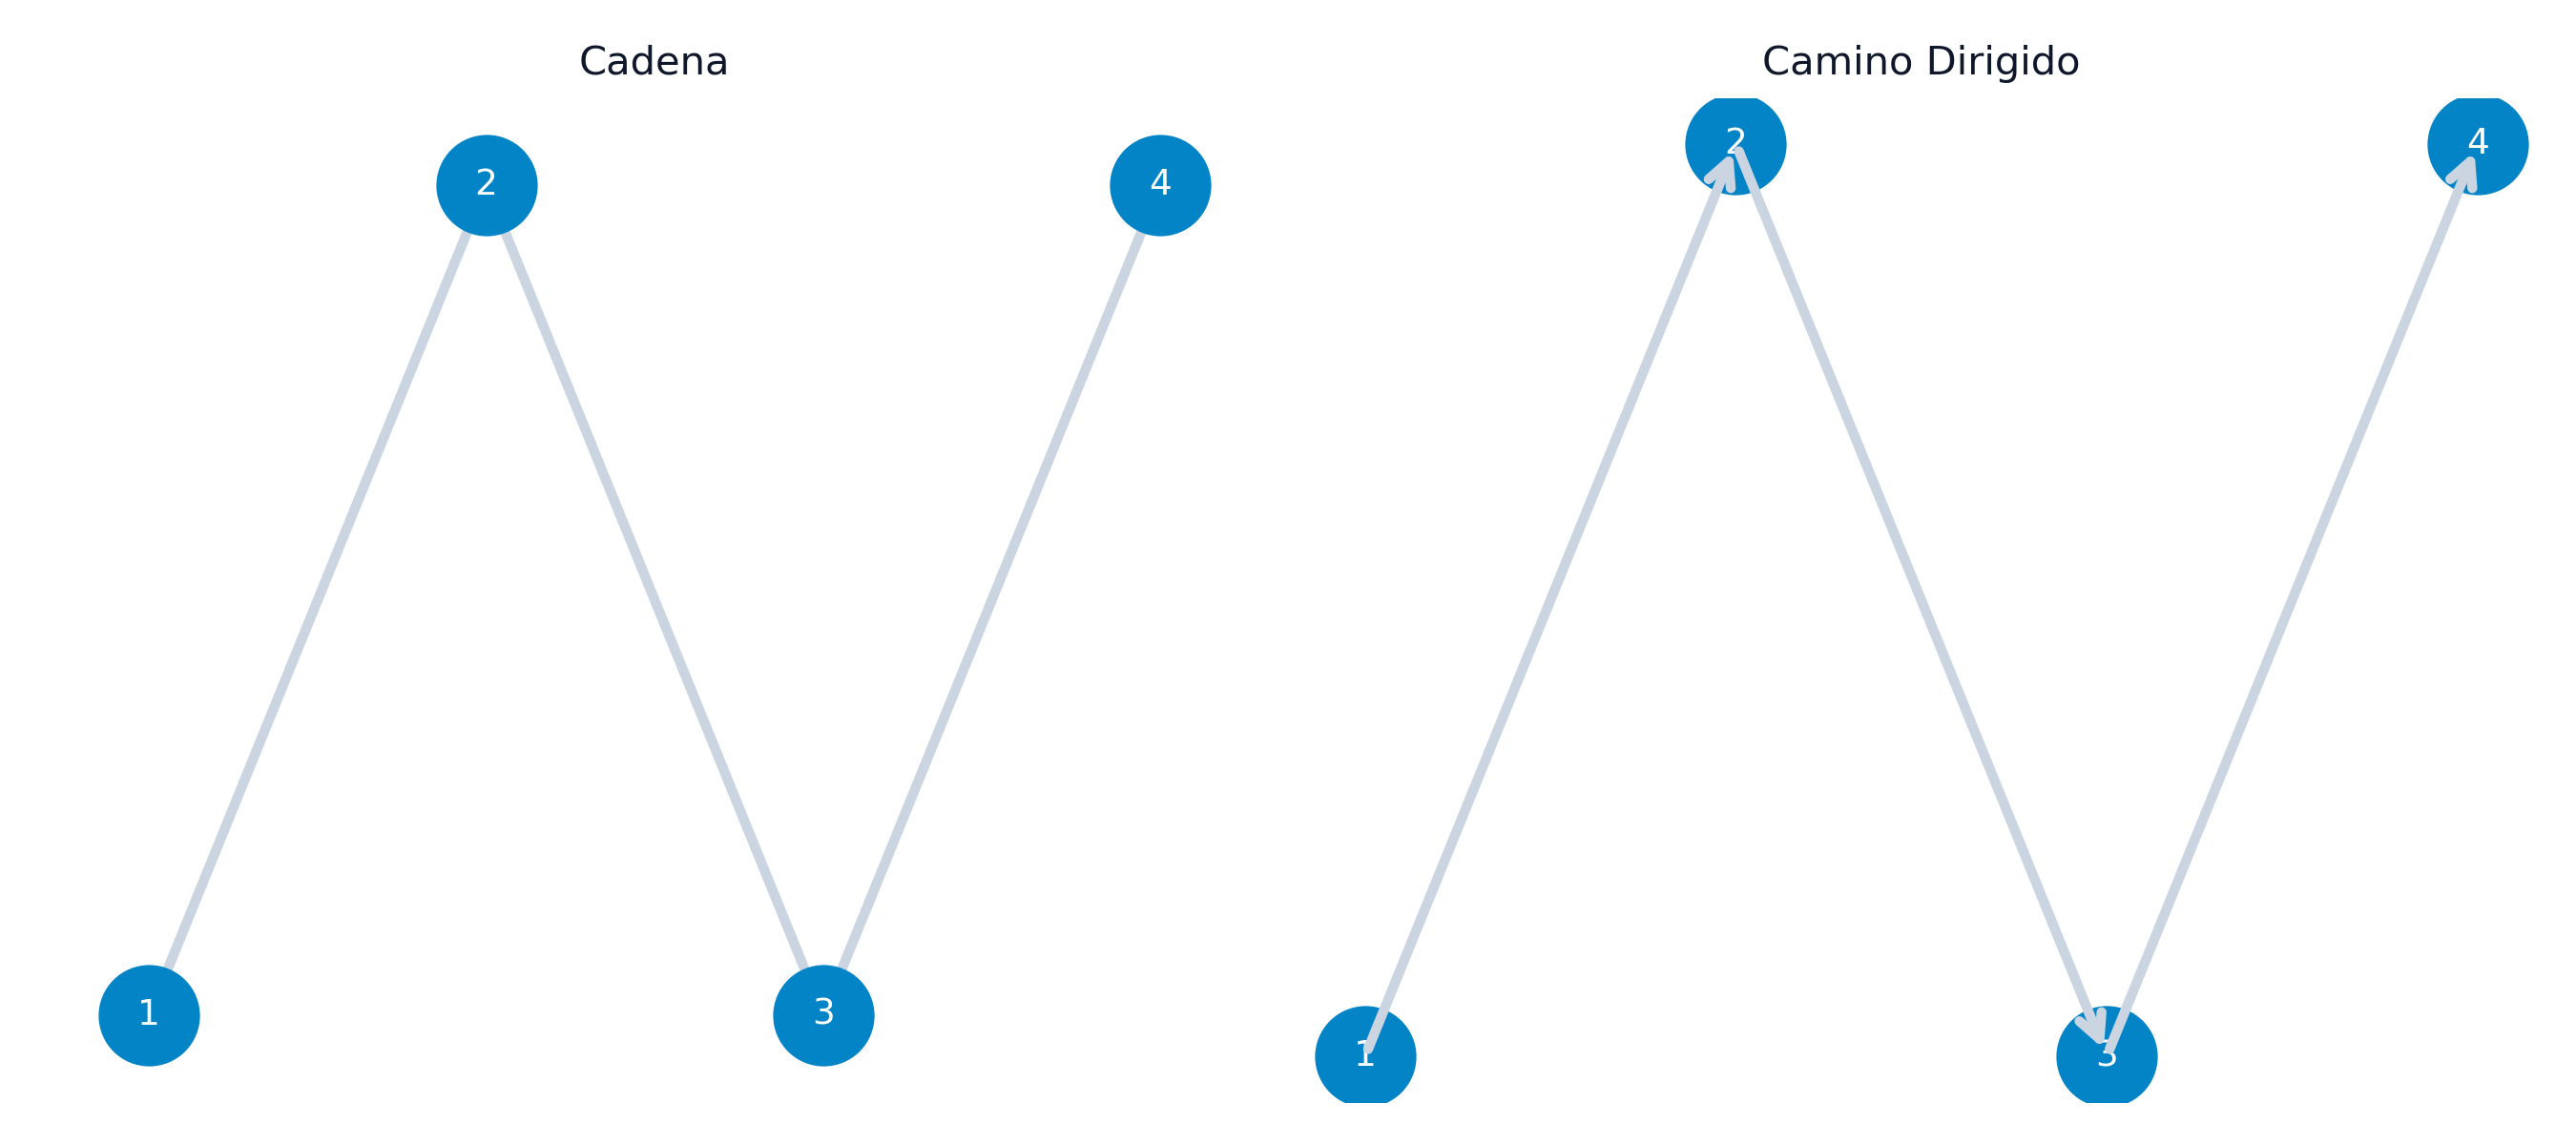
\includegraphics[width=0.75\linewidth,height=\textheight,keepaspectratio]{images/cadenas_caminos_diferencia.png}

}

\caption{\label{fig-caminos-clasificacion-animado}Clasificación de
caminos dirigidos según su elementalidad y simplicidad}

\end{figure}%

\end{tcolorbox}

Además del estudio de la elementalidad y la simplicidad de las cadenas,
la cuantificación de la métrica de los recorridos permite caracterizar
la extensión global y la compacidad de una red.

\begin{tcolorbox}[enhanced jigsaw, toprule=.15mm, opacitybacktitle=0.6, coltitle=black, colbacktitle=quarto-callout-note-color!10!white, title=\textcolor{quarto-callout-note-color}{\faInfo}\hspace{0.5em}{Definición: Longitud, distancia geodésica y diámetro}, arc=.35mm, rightrule=.15mm, toptitle=1mm, breakable, bottomtitle=1mm, titlerule=0mm, colback=white, opacityback=0, leftrule=.75mm, colframe=quarto-callout-note-color-frame, left=2mm, bottomrule=.15mm]

Dado un digrafo \(G = (V, U)\) (o grafo \(G = (V, E)\)):

\begin{itemize}
\item
  \textbf{Longitud de una Cadena}: Número exacto de arcos o aristas
  \(q\) que componen la secuencia \(\mu\).
\item
  \textbf{Distancia Geodésica \(d(i, j)\)}: Longitud de la cadena más
  corta existente entre el nodo \(i\) y el nodo \(j\).
\item
  \textbf{Diámetro de un Grafo \(D(G)\)}: Mayor distancia geodésica
  entre cualquier par de nodos de la red: \[
  D(G) = \max_{i, j \in V} d(i, j)
  \]
\end{itemize}

\end{tcolorbox}

En la Figura~\ref{fig-diametro-grafo} se ilustra la evaluación del
diámetro sobre la red orientada de 5 nodos \(V = \{1, 2, 3, 4, 5\}\). Al
analizar la distancia geodésica entre cada par de vértices (como la
conexión entre los nodos 1 y 4 a través de la cadena de 2 arcos
\(\{(1,2), (2,4)\}\), o entre los nodos 3 y 4 a través de
\(\{(3,2), (2,4)\}\)), se comprueba que la máxima distancia necesaria
para comunicar cualquier pareja de nodos en la red es de 2 arcos. Por
consiguiente, el diámetro global del grafo es \(D(G) = 2\).

\begin{figure}

\centering{

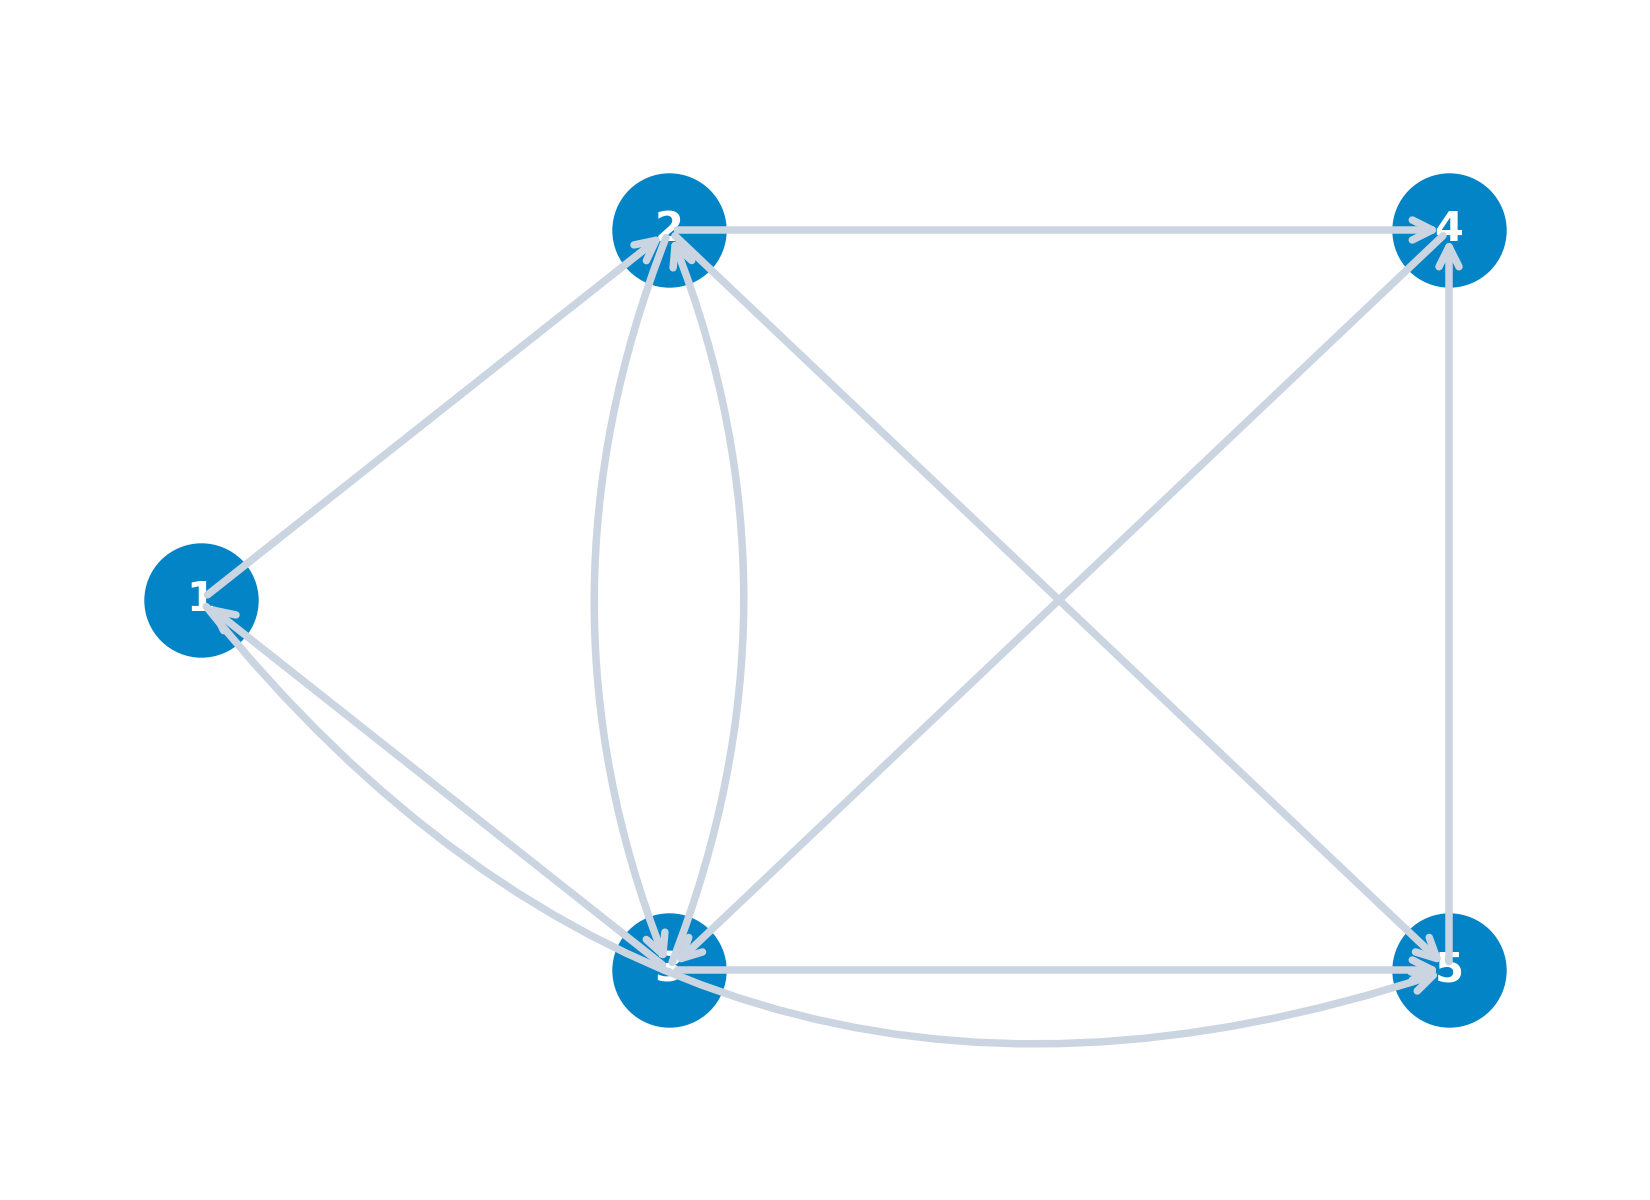
\includegraphics[width=0.55\linewidth,height=\textheight,keepaspectratio]{images/diametro_grafo_ejemplo.png}

}

\caption{\label{fig-diametro-grafo}Evaluación del diámetro D(G)=2 sobre
una red orientada de 5 vértices}

\end{figure}%

\begin{tcolorbox}[enhanced jigsaw, toprule=.15mm, opacitybacktitle=0.6, coltitle=black, colbacktitle=quarto-callout-warning-color!10!white, title=\textcolor{quarto-callout-warning-color}{\faExclamationTriangle}\hspace{0.5em}{Advertencia: Diferencia fundamental entre cadena y camino}, arc=.35mm, rightrule=.15mm, toptitle=1mm, breakable, bottomtitle=1mm, titlerule=0mm, colback=white, opacityback=0, leftrule=.75mm, colframe=quarto-callout-warning-color-frame, left=2mm, bottomrule=.15mm]

Para sintetizar las propiedades de recorrido en redes orientadas y no
dirigidas, conviene destacar la distinción conceptual entre cadena y
camino:

\begin{itemize}
\item
  \textbf{Cadena}: Secuencia de arcos o aristas adyacentes que
  \textbf{no exige respetar la orientación de las flechas}. Los arcos
  pueden recorrerse tanto en sentido directo como en sentido inverso.
  Caracteriza la \textbf{conectividad puramente sintáctica o topológica}
  entre dos nodos.
\item
  \textbf{Camino}: Secuencia de arcos orientados en la que \textbf{todos
  los arcos se transitan estrictamente en el sentido de su flecha} (el
  nodo destino del \(k\)-ésimo arco es el nodo origen del
  \((k+1)\)-ésimo). Describe la \textbf{posibilidad real de circulación
  de flujo o transporte} en la red.
\end{itemize}

En consecuencia, \textbf{todo camino dirigido es una cadena}, pero
\textbf{no toda cadena constituye un camino}. En redes no dirigidas
(donde las aristas carecen de orientación), las nociones de cadena y
camino resultan formalmente equivalentes.

\end{tcolorbox}

\subsection{Conectividad}\label{conectividad}

La accesibilidad entre los vértices determina la capacidad global de
comunicación e integridad estructural de una red. En grafos no
dirigidos, la existencia de recorridos entre sus nodos permite definir
la noción de conexidad global, mientras que en redes orientadas es
preciso distinguir entre la mera conectividad sintáctica (existencia de
cadenas) y la conectividad efectiva de transporte (existencia de caminos
dirigidos).

\begin{tcolorbox}[enhanced jigsaw, toprule=.15mm, opacitybacktitle=0.6, coltitle=black, colbacktitle=quarto-callout-note-color!10!white, title=\textcolor{quarto-callout-note-color}{\faInfo}\hspace{0.5em}{Definición: Grafo conexo y digrafo fuertemente conexo}, arc=.35mm, rightrule=.15mm, toptitle=1mm, breakable, bottomtitle=1mm, titlerule=0mm, colback=white, opacityback=0, leftrule=.75mm, colframe=quarto-callout-note-color-frame, left=2mm, bottomrule=.15mm]

Dado un grafo \(G = (V, E)\) o digrafo \(G = (V, U)\):

\begin{itemize}
\item
  \textbf{Grafo Conexo}: Un grafo no dirigido es \textbf{conexo} si
  entre cualquier par de vértices \(i, j \in V\) existe al menos una
  \textbf{cadena}.
\item
  \textbf{Digrafo Fuertemente Conexo}: Un digrafo es \textbf{fuertemente
  conexo} si entre cualquier par de vértices \(i, j \in V\) existe al
  menos un \textbf{camino dirigido} en ambas direcciones (de \(i\) a
  \(j\) y de \(j\) a \(i\)).
\end{itemize}

\end{tcolorbox}

En la Figura~\ref{fig-digrafo-conexidad} se ilustra un digrafo sobre 7
vértices \(V = \{a, b, c, d, e, f, g\}\). Este digrafo resulta ser
\textbf{conexo} en el sentido débil (al existir cadenas no orientadas
que comunican todos los nodos), pero \textbf{no es fuertemente conexo}.
El vértice \(d\) actúa como un nodo sumidero al que convergen únicamente
arcos entrantes desde \(a, c, g\), impidiendo la existencia de cualquier
camino saliente que conecte a \(d\) con los demás vértices de la red.

\begin{figure}

\centering{

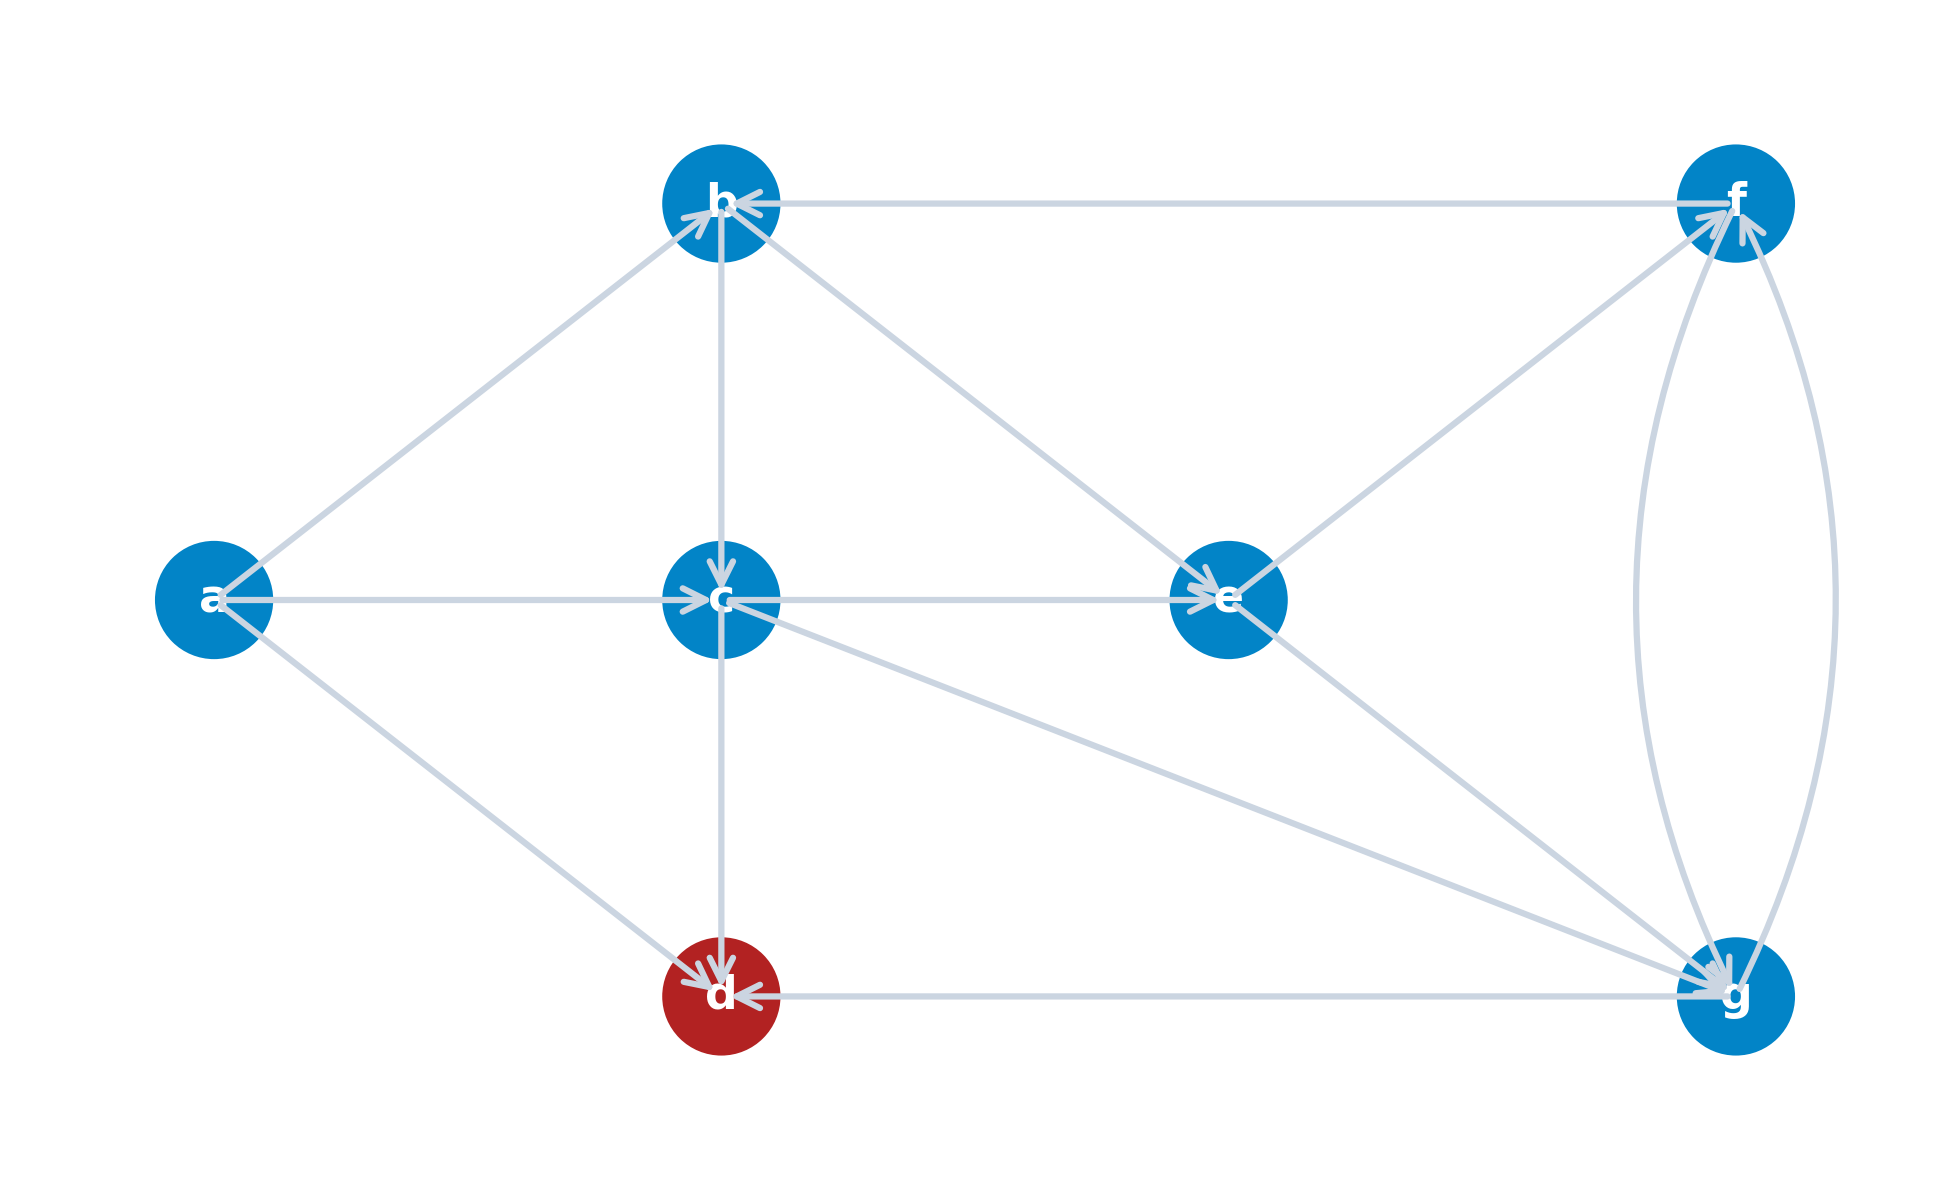
\includegraphics[width=0.6\linewidth,height=\textheight,keepaspectratio]{images/digrafo_conexidad_ejemplo.png}

}

\caption{\label{fig-digrafo-conexidad}Digrafo conexo pero no fuertemente
conexo con nodo sumidero en d}

\end{figure}%

Cuando una red carece de conexidad global, esta se disgrega de forma
natural en subgrafos independientes aislados denominados
\textbf{componentes conexas}. Esta descomposición se formaliza
rigurosamente mediante la definición de una relación de equivalencia
sobre el conjunto de vértices.

\begin{tcolorbox}[enhanced jigsaw, toprule=.15mm, opacitybacktitle=0.6, coltitle=black, colbacktitle=quarto-callout-note-color!10!white, title=\textcolor{quarto-callout-note-color}{\faInfo}\hspace{0.5em}{Definición: Relación de conexidad y componentes conexas}, arc=.35mm, rightrule=.15mm, toptitle=1mm, breakable, bottomtitle=1mm, titlerule=0mm, colback=white, opacityback=0, leftrule=.75mm, colframe=quarto-callout-note-color-frame, left=2mm, bottomrule=.15mm]

En un grafo \(G = (V, E)\) o digrafo \(G = (V, U)\), se define la
relación binaria \(R\) sobre el conjunto de vértices \(V\): \[
\forall i, j \in V, \quad i \, R \, j \iff \exists \text{ una cadena entre } i \text{ y } j
\]

La relación \(R\) constituye una \textbf{relación de equivalencia} al
satisfacer tres propiedades fundamentales:

\begin{itemize}
\item
  \textbf{Reflexiva}: Todo nodo está relacionado consigo mismo
  (\(i \, R \, i\)) mediante una cadena trivial de longitud 0.
\item
  \textbf{Simétrica}: Si existe una cadena de \(i\) a \(j\), invirtiendo
  el orden de recorrido se obtiene una cadena de \(j\) a \(i\)
  (\(i \, R \, j \implies j \, R \, i\)).
\item
  \textbf{Transitiva}: Si existe una cadena de \(i\) a \(j\) y otra de
  \(j\) a \(k\), la concatenación de ambas forma una cadena de \(i\) a
  \(k\) (\(i \, R \, j \land j \, R \, k \implies i \, R \, k\)).
\end{itemize}

Las clases de equivalencia inducidas por \(R\) sobre \(V\) determinan la
partición del grafo en sus \textbf{componentes conexas}.

\end{tcolorbox}

En la Figura~\ref{fig-componentes-conexas-dos} se presenta un grafo
descompuesto en dos componentes conexas disjuntas: la primera integrada
por los vértices \(\{a, b, c, d\}\) con las aristas
\(\{\{a,b\}, \{b,c\}, \{c,d\}, \{b,d\}\}\), y la segunda constituida por
los vértices \(\{e, f, g\}\) con las aristas \(\{\{e,f\}, \{f,g\}\}\).

\begin{figure}

\centering{

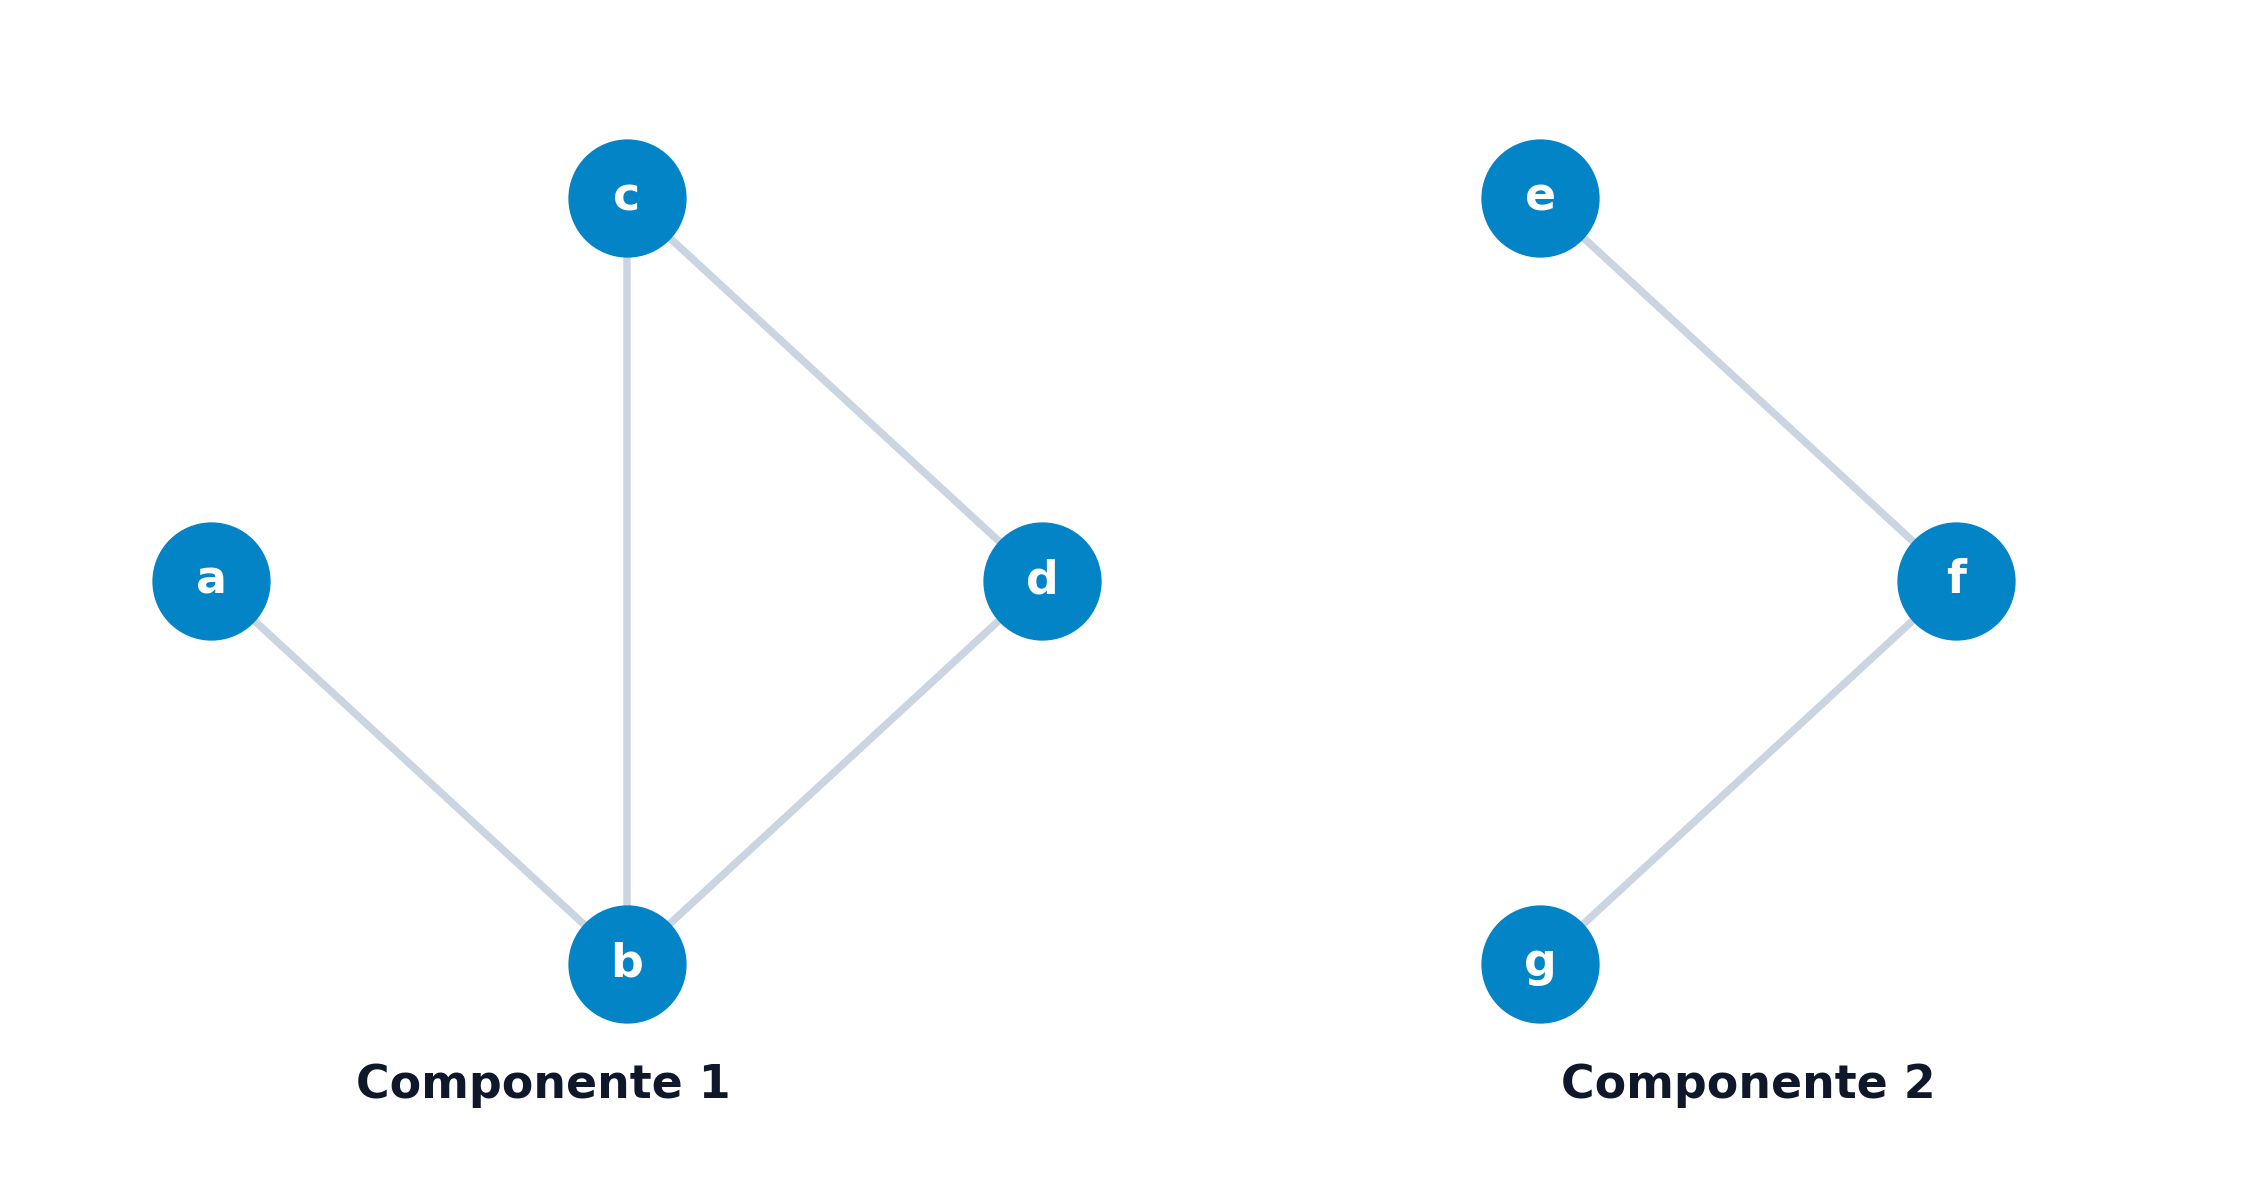
\includegraphics[width=0.65\linewidth,height=\textheight,keepaspectratio]{images/componentes_conexas_dos.png}

}

\caption{\label{fig-componentes-conexas-dos}Grafo no dirigido
descompuesto en dos componentes conexas disjuntas}

\end{figure}%

El análisis de los recorridos cerrados, aquellos cuyo vértice inicial y
final coinciden, permite caracterizar la presencia de redundancias en la
red y definir los grafos conexos acíclicos, denominados
\textbf{árboles}, que desempeñan un papel central en la optimización de
infraestructuras.

\begin{tcolorbox}[enhanced jigsaw, toprule=.15mm, opacitybacktitle=0.6, coltitle=black, colbacktitle=quarto-callout-note-color!10!white, title=\textcolor{quarto-callout-note-color}{\faInfo}\hspace{0.5em}{Definición: Ciclo, bucle, circuito y árbol}, arc=.35mm, rightrule=.15mm, toptitle=1mm, breakable, bottomtitle=1mm, titlerule=0mm, colback=white, opacityback=0, leftrule=.75mm, colframe=quarto-callout-note-color-frame, left=2mm, bottomrule=.15mm]

Dado un grafo \(G = (V, E)\) o digrafo \(G = (V, U)\):

\begin{itemize}
\item
  \textbf{Ciclo}: Una \textbf{cadena simple} cuyo nodo inicial y nodo
  final coinciden (\(v_0 = v_k\)).
\item
  \textbf{Bucle}: Un ciclo formado por una única arista o arco que
  conecta un vértice consigo mismo.
\item
  \textbf{Circuito}: Un \textbf{camino simple} en el que el nodo inicial
  y el nodo final coinciden (\(v_0 = v_k\)).
\item
  \textbf{Árbol}: Un \textbf{grafo conexo sin ciclos}.
\end{itemize}

\end{tcolorbox}

En la Figura~\ref{fig-arboles-ciclos-ejemplos} se comparan dos
estructuras topológicas básicas: a la izquierda, un grafo que contiene
el ciclo elemental en triángulo \(\{\{a,b\}, \{b,c\}, \{c,a\}\}\); a la
derecha, una red en estrella centrada en el nodo \(a\) conectada a 8
vértices periféricos \(\{b, c, d, e, f, g, h, i\}\) que constituye un
árbol conexo acíclico.

\begin{figure}

\centering{

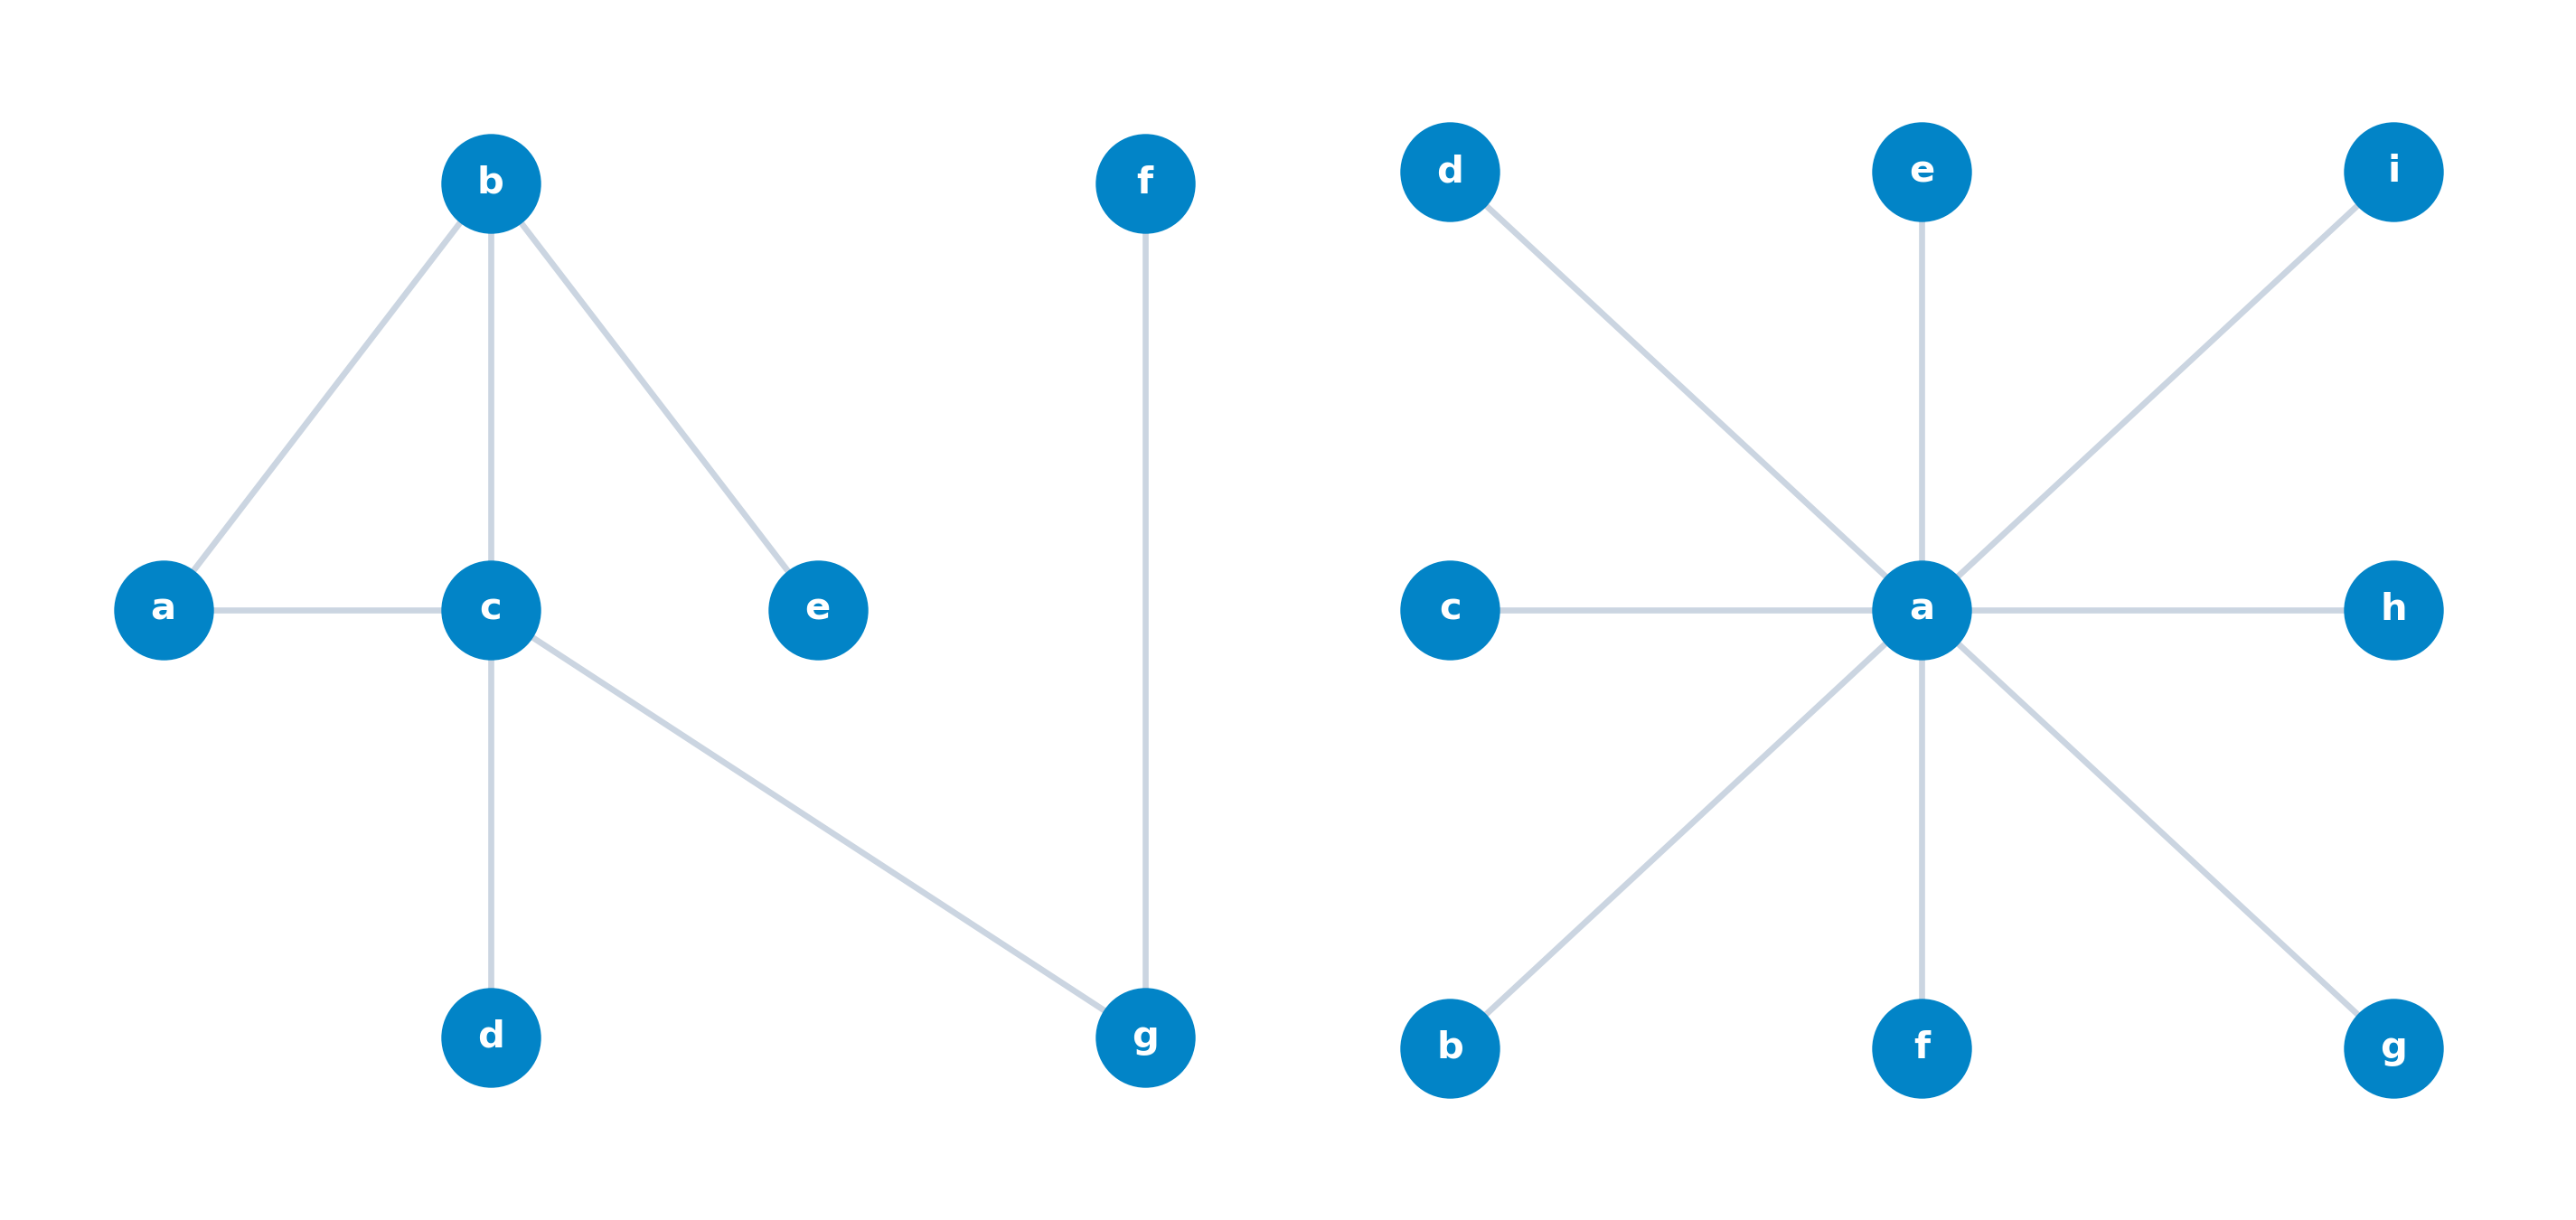
\includegraphics[width=0.85\linewidth,height=\textheight,keepaspectratio]{images/arboles_ciclos_ejemplos.png}

}

\caption{\label{fig-arboles-ciclos-ejemplos}Comparación entre un grafo
no dirigido con ciclo y un árbol en estrella acíclico}

\end{figure}%

La presencia de ciclos impone restricciones estructurales muy precisas
sobre los grados de los vértices y la conectividad del grafo, recogidas
en el siguiente teorema.

\begin{tcolorbox}[enhanced jigsaw, toprule=.15mm, opacitybacktitle=0.6, coltitle=black, colbacktitle=quarto-callout-important-color!10!white, title=\textcolor{quarto-callout-important-color}{\faExclamation}\hspace{0.5em}{Teorema: Propiedades estructurales de los ciclos y árboles}, arc=.35mm, rightrule=.15mm, toptitle=1mm, breakable, bottomtitle=1mm, titlerule=0mm, colback=white, opacityback=0, leftrule=.75mm, colframe=quarto-callout-important-color-frame, left=2mm, bottomrule=.15mm]

Para todo grafo conexo \(G = (V, E)\) con \(n = |V| > 1\) vértices, se
verifican las siguientes propiedades fundamentales:

\begin{enumerate}
\def\labelenumi{\arabic{enumi}.}
\item
  \textbf{Ausencia de vértices pendientes}: Si \(G\) no posee vértices
  pendientes (es decir, todos sus nodos tienen grado
  \(\delta(v) \ge 2\)), entonces \(G\) contiene \textbf{al menos un
  ciclo}.
\item
  \textbf{Existencia de hojas en árboles}: Si \(G\) es un árbol conexo
  sin ciclos, entonces \(G\) contiene \textbf{al menos un vértice
  pendiente} (hoja con \(\delta(v) = 1\)).
\item
  \textbf{Caracterización de aristas en ciclos}: Una arista \(e \in E\)
  pertenece a un ciclo \(\mu\) de \(G\) si y solo si su eliminación no
  desconecta el grafo; es decir, \(G \setminus \{e\}\) continúa siendo
  un grafo conexo.
\end{enumerate}

\end{tcolorbox}

Estas propiedades estructurales constituyen el fundamento sobre el que
se edifican los algoritmos de búsqueda y construcción de árboles de
expansión mínima (como los algoritmos de Kruskal y Prim) que se
estudiarán en las secciones posteriores.

\begin{center}\rule{0.5\linewidth}{0.5pt}\end{center}

\section{Grafos planares y grafos
bipartitos}\label{grafos-planares-y-grafos-bipartitos}

Una propiedad fundamental en el estudio topológico de redes es la
capacidad de representar un grafo geométricamente sobre el plano
bidimensional \(\mathbb{R}^2\) de manera que sus aristas no se
intersecten. La disposición geométrica sobre el plano resulta crítica en
aplicaciones reales como el diseño de circuitos impresos (PCB), el
trazado de mapas de carreteras o la canalización de infraestructuras
subterráneas de transporte de energía y fluidos.

\begin{tcolorbox}[enhanced jigsaw, toprule=.15mm, opacitybacktitle=0.6, coltitle=black, colbacktitle=quarto-callout-note-color!10!white, title=\textcolor{quarto-callout-note-color}{\faInfo}\hspace{0.5em}{Definición: Grafo planar e incrustación planar}, arc=.35mm, rightrule=.15mm, toptitle=1mm, breakable, bottomtitle=1mm, titlerule=0mm, colback=white, opacityback=0, leftrule=.75mm, colframe=quarto-callout-note-color-frame, left=2mm, bottomrule=.15mm]

Un grafo \(G = (V, E)\) se denomina \textbf{planar} si admite una
representación geométrica en el plano bidimensional de modo que sus
aristas no se crucen ni se corten entre sí en ningún punto distinto de
sus vértices extremos.

Se denomina \textbf{incrustación planar} a cualquier dibujo plano de
\(G\) exento de intersecciones entre aristas. Una incrustación planar
divide el plano en subconjuntos conexos acotados y no acotados
denominados \textbf{caras} o \textbf{regiones} \(r\). Todo grafo planar
posee exactamente \textbf{una región exterior no acotada}.

\end{tcolorbox}

Un mismo grafo abstracto admite múltiples diagramaciones geométricas
sobre el plano. En la Figura~\ref{fig-k4-planaridad} se ilustra esta
propiedad mediante el grafo completo sobre 4 vértices \(K_4\): la
representación convencional de la izquierda presenta dos aristas
diagonales cruzándose en un punto central; sin embargo, al recolocar el
vértice \(a\) en la región interior acotada por el triángulo
\(\{b, c, d\}\) (representación derecha), se obtiene un dibujo
equivalente exento de intersecciones. Por tanto, el grafo completo
\(K_4\) es \textbf{planar}.

\begin{figure}

\centering{

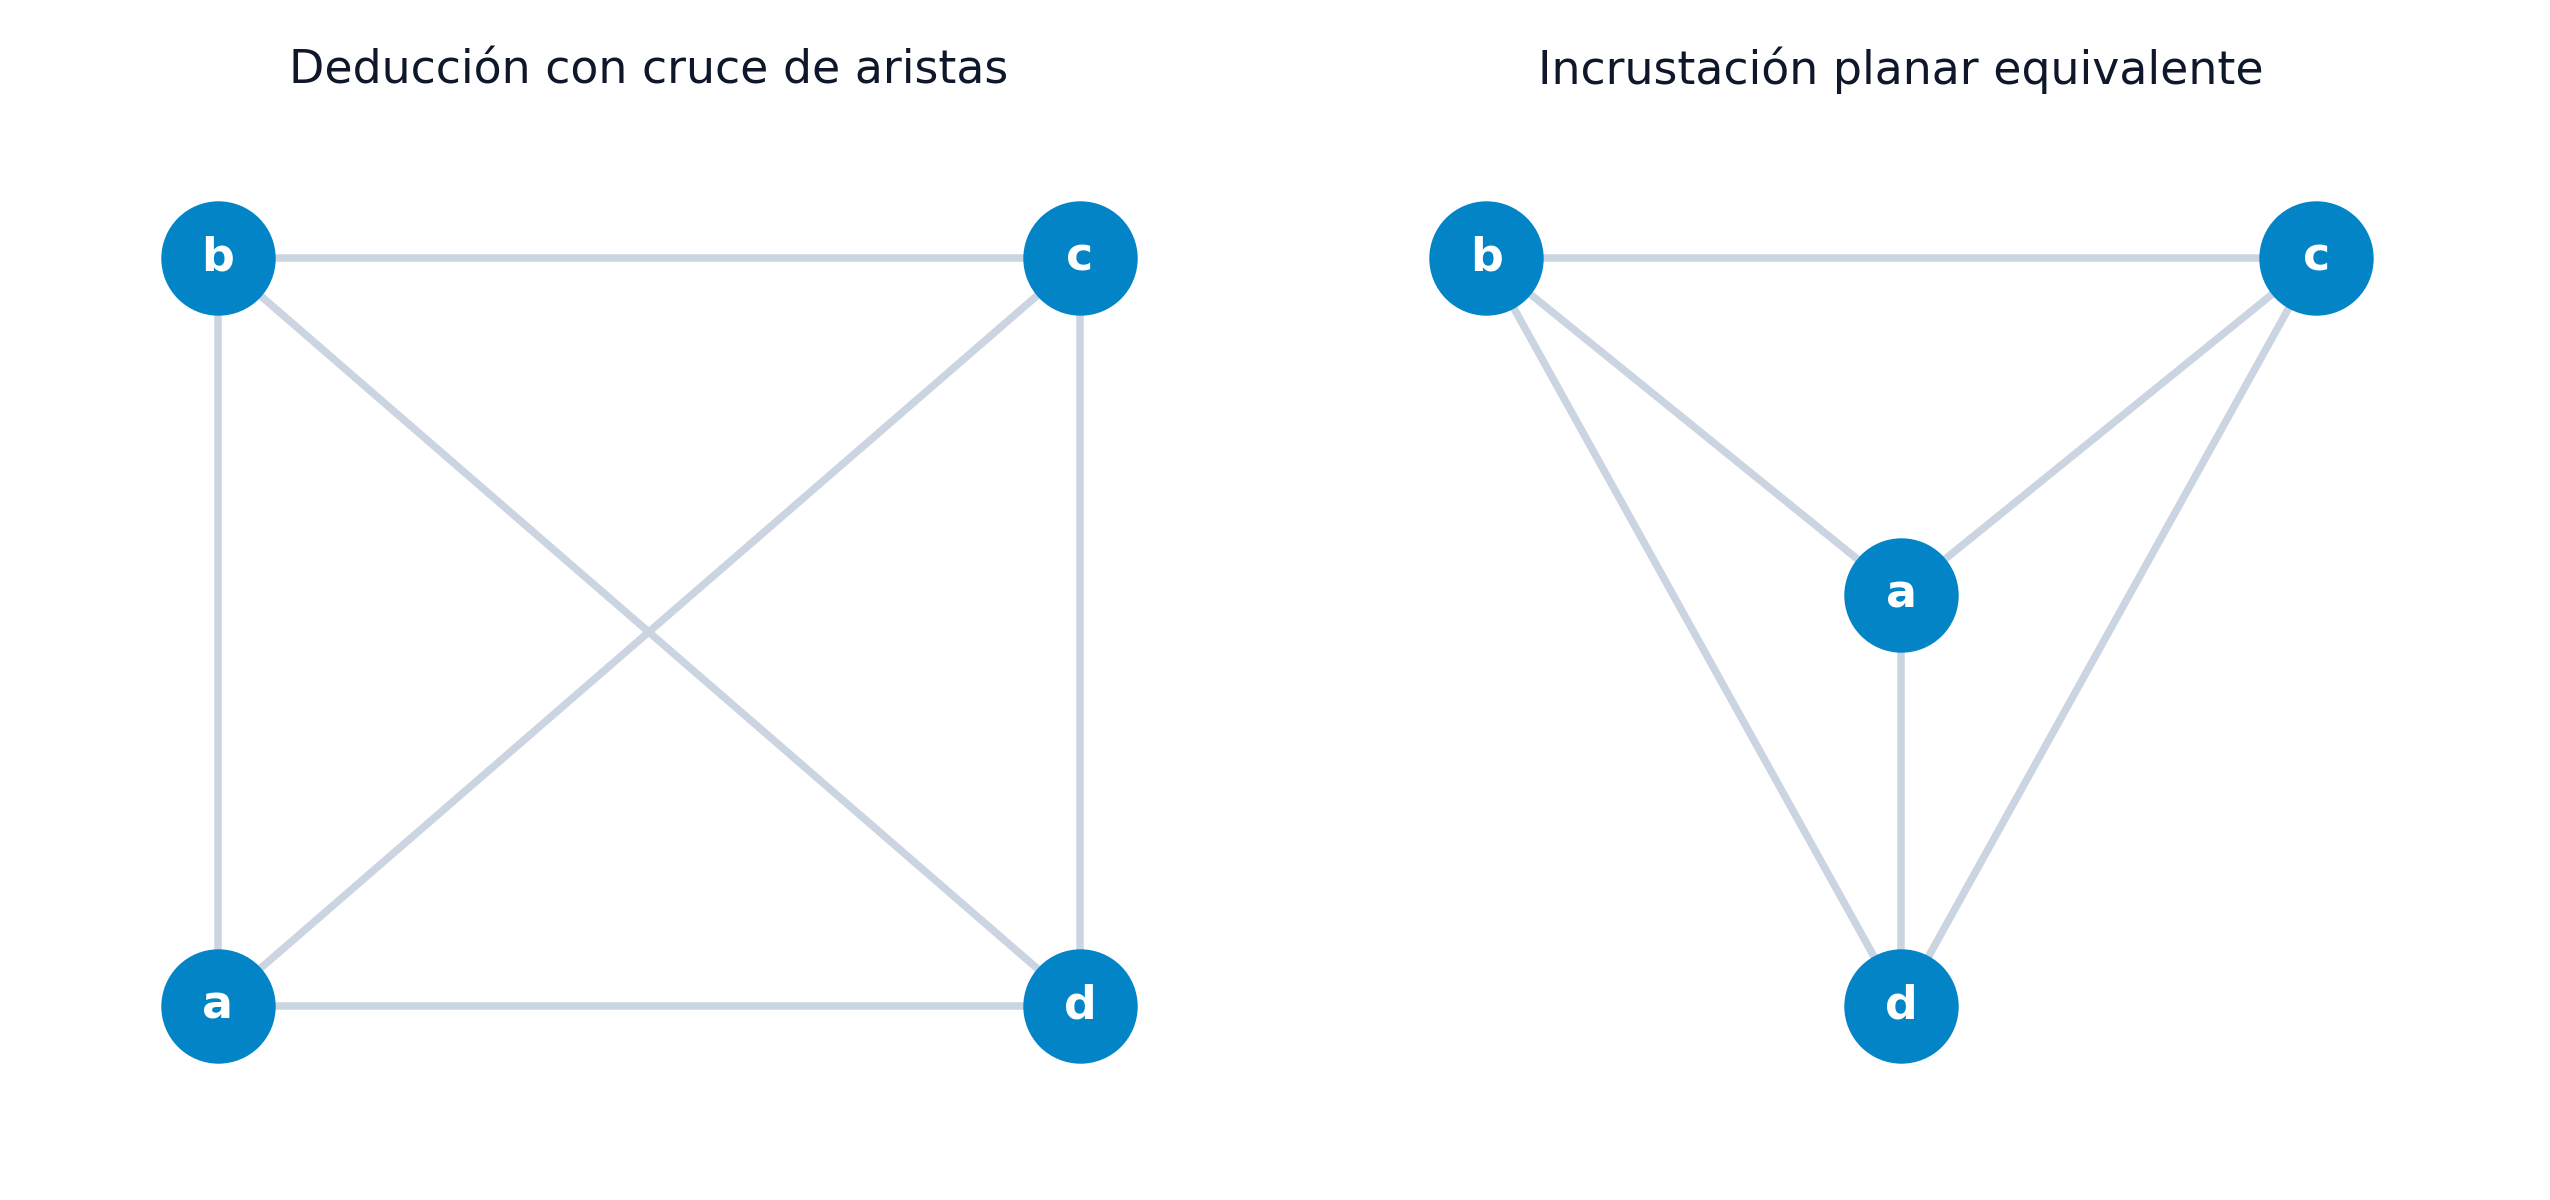
\includegraphics[width=0.75\linewidth,height=\textheight,keepaspectratio]{images/k4_planaridad_ejemplo.png}

}

\caption{\label{fig-k4-planaridad}Planaridad del grafo completo K4
mediante incrustación equivalente sin cruces}

\end{figure}%

Los grafos completos de menor orden (\(K_2, K_3, K_4\)) son todos
planares. Sin embargo, al incrementar el número de vértices, la
saturación de conexiones impide mantener la planaridad. En 1840, el
matemático August Möbius planteó esta limitación mediante un célebre
problema acertijo:

\begin{quote}
\emph{``Un rey ordenó en su testamento que, tras su muerte, su reino
fuera dividido entre sus 5 hijos en 5 regiones contiguas de forma que
cada región tuviera frontera común con todas las demás 4 regiones. ¿Es
posible cumplir la voluntad del rey?''}
\end{quote}

La respuesta matemática es \textbf{negativa}. El cumplimiento del
testamento requeriría la existencia de un mapa cuyo grafo dual de
fronteras fuera un grafo completo con 5 vértices, \(K_5\), en el que
cada par de vértices tuviera una arista de colindancia. Como se ilustra
en la Figura~\ref{fig-k5-mobius}, el grafo completo \(K_5\) (con 5
vértices y 10 aristas) resulta ser un \textbf{grafo no planar}, puesto
que cualquier intento de incrustar sus aristas en el plano genera al
menos un cruce inevitable.

\begin{figure}

\centering{

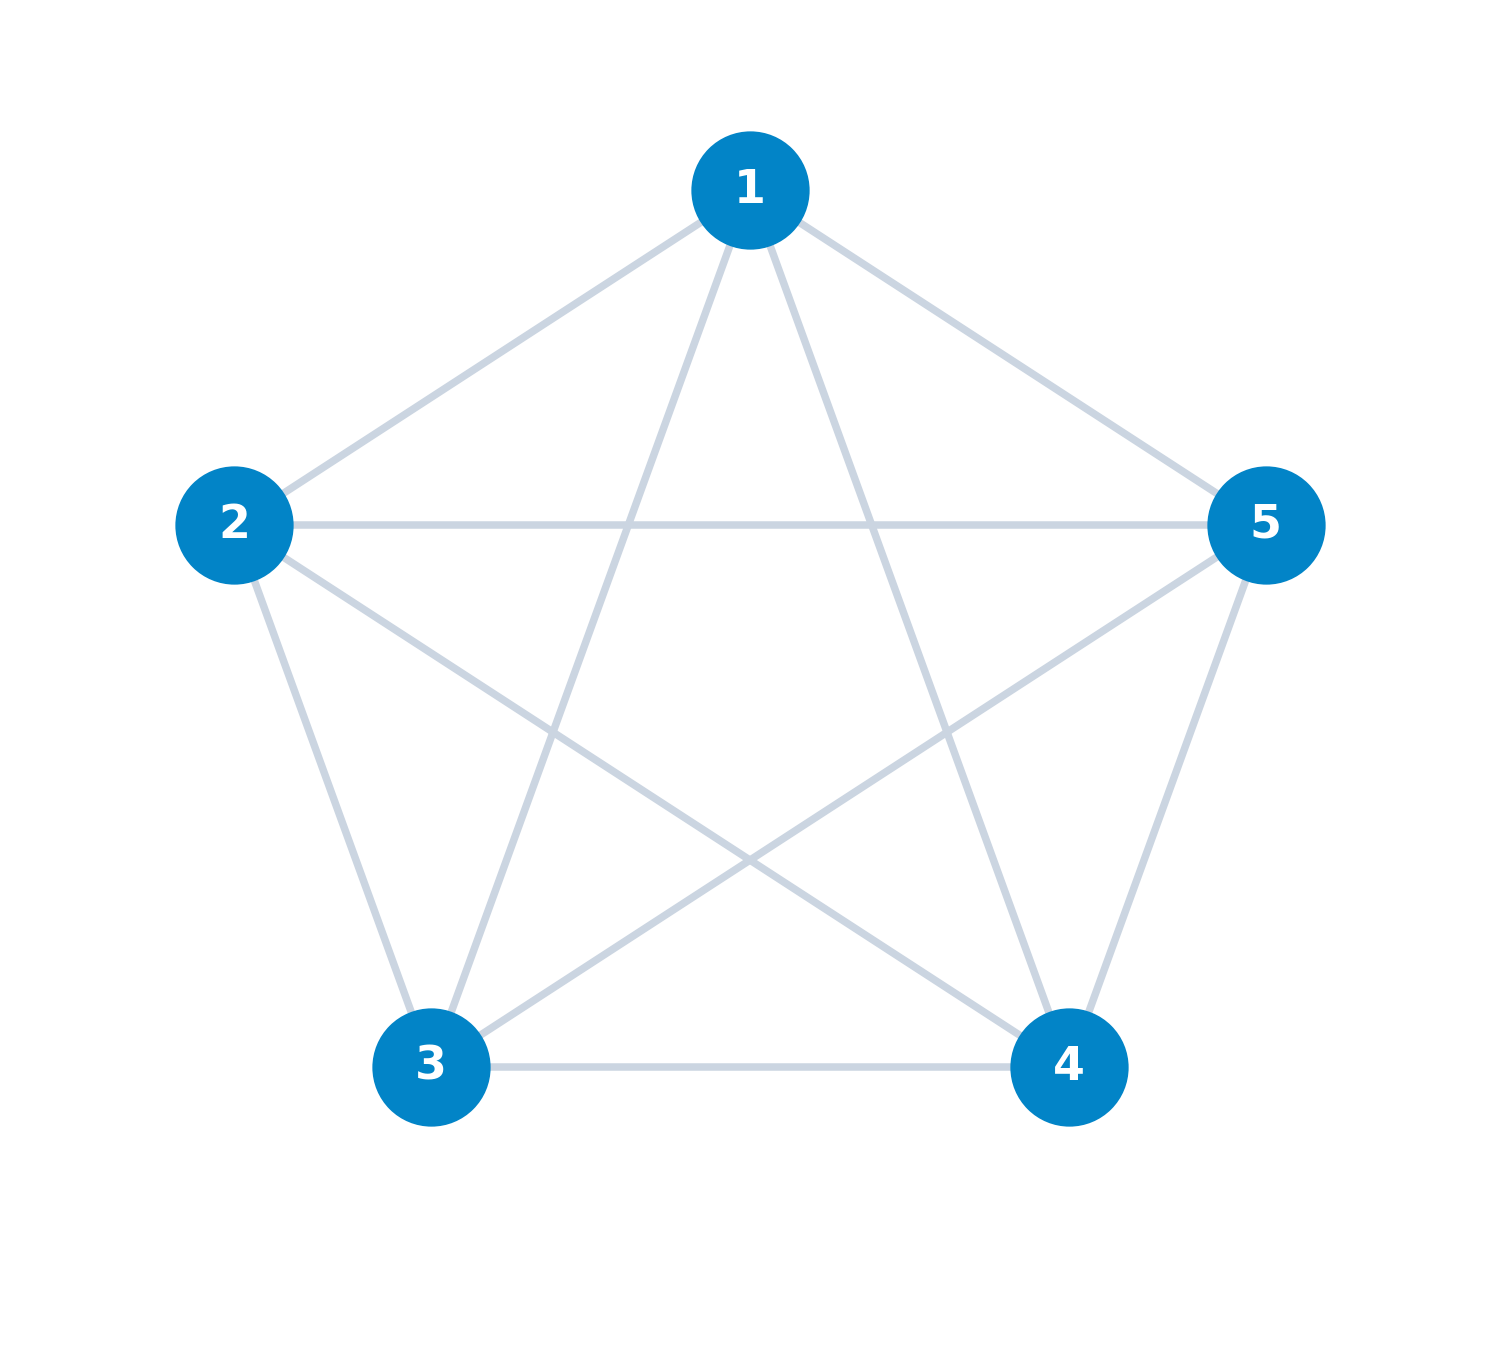
\includegraphics[width=0.45\linewidth,height=\textheight,keepaspectratio]{images/k5_mobius_problema.png}

}

\caption{\label{fig-k5-mobius}El grafo completo K5 y el problema de las
5 regiones de Möbius (no planar)}

\end{figure}%

Además de los grafos completos, existe otra importante familia de redes
asociadas a problemas de asignación e interconexión: los \textbf{grafos
bipartitos}.

\begin{tcolorbox}[enhanced jigsaw, toprule=.15mm, opacitybacktitle=0.6, coltitle=black, colbacktitle=quarto-callout-note-color!10!white, title=\textcolor{quarto-callout-note-color}{\faInfo}\hspace{0.5em}{Definición: Grafo bipartito y bipartito completo}, arc=.35mm, rightrule=.15mm, toptitle=1mm, breakable, bottomtitle=1mm, titlerule=0mm, colback=white, opacityback=0, leftrule=.75mm, colframe=quarto-callout-note-color-frame, left=2mm, bottomrule=.15mm]

Un grafo \(G = (V, E)\) es \textbf{bipartito} si su conjunto de vértices
admite una partición en dos subconjuntos disjuntos: \[
V = V_1 \cup V_2, \quad V_1 \cap V_2 = \emptyset
\] de modo que toda arista de \(E\) conecta un vértice de \(V_1\) con un
vértice de \(V_2\) (no existen aristas uniendo vértices dentro del mismo
subconjunto).

Un \textbf{grafo bipartito completo} \(K_{n_1, n_2}\) es un grafo
bipartito con \(|V_1| = n_1\) y \(|V_2| = n_2\) que contiene todas las
\(n_1 \cdot n_2\) aristas posibles entre ambos subconjuntos: \[
\{v_1, v_2\} \in E, \quad \forall v_1 \in V_1, \, \forall v_2 \in V_2
\]

\end{tcolorbox}

Una propiedad estructural fundamental que caracteriza analíticamente a
la familia de los grafos bipartitos se formaliza en el siguiente
teorema:

\begin{tcolorbox}[enhanced jigsaw, toprule=.15mm, opacitybacktitle=0.6, coltitle=black, colbacktitle=quarto-callout-important-color!10!white, title=\textcolor{quarto-callout-important-color}{\faExclamation}\hspace{0.5em}{Teorema: Caracterización de grafos bipartitos}, arc=.35mm, rightrule=.15mm, toptitle=1mm, breakable, bottomtitle=1mm, titlerule=0mm, colback=white, opacityback=0, leftrule=.75mm, colframe=quarto-callout-important-color-frame, left=2mm, bottomrule=.15mm]

Un grafo \(G = (V, E)\) es \textbf{bipartito} si y solo si \textbf{no
contiene ningún ciclo de longitud impar}.

\end{tcolorbox}

El análisis de la planaridad en grafos bipartitos se halla
históricamente ligado al célebre \emph{Problema de los tres servicios}
(suministro de agua \(A\), gas \(G\) y electricidad \(E\) a tres casas
\(C_1, C_2, C_3\)), popularizado por Henry Ernest Dudeney (Dudeney
1958):

\begin{quote}
\emph{``¿Es posible canalizar las conducciones subterráneas de tres
suministros esenciales (agua, gas y electricidad) hacia tres viviendas
independientes de modo que ninguna tubería o cable se cruce con otro en
el plano?''}
\end{quote}

Desde la perspectiva de la teoría de redes, este acertijo plantea
formalmente si el grafo bipartito completo \(K_{3,3}\) (formado por
\(n_1=3\) fuentes de suministro y \(n_2=3\) casas, sumando \(n=6\)
vértices y \(m=9\) aristas) admite o no una incrustación planar.

Como se ilustra en la Figura~\ref{fig-k33-bipartito}, la disposición
bipartita estándar en dos columnas paralelas (a la izquierda) exhibe de
forma explícita la saturación de conexiones (\(3 \times 3 = 9\) aristas)
con múltiples cruces inevitables. Incluso si se intenta reorganizar
libremente la posición de los vértices en el plano (a la derecha) para
trazar las conducciones mediante trayectorias curvas bordeando los
nodos, se comprueba que tras conectar exitosamente 8 de los trazados, la
novena arista queda confina dentro de una región delimitada por las
conducciones anteriores, resultando imposible completar el tendido sin
interceptar una arista preexistente. En consecuencia, la respuesta al
acertijo de Dudeney es \textbf{negativa} y se concluye que el grafo
bipartito completo \(K_{3,3}\) es un \textbf{grafo no planar}.

\begin{figure}

\centering{

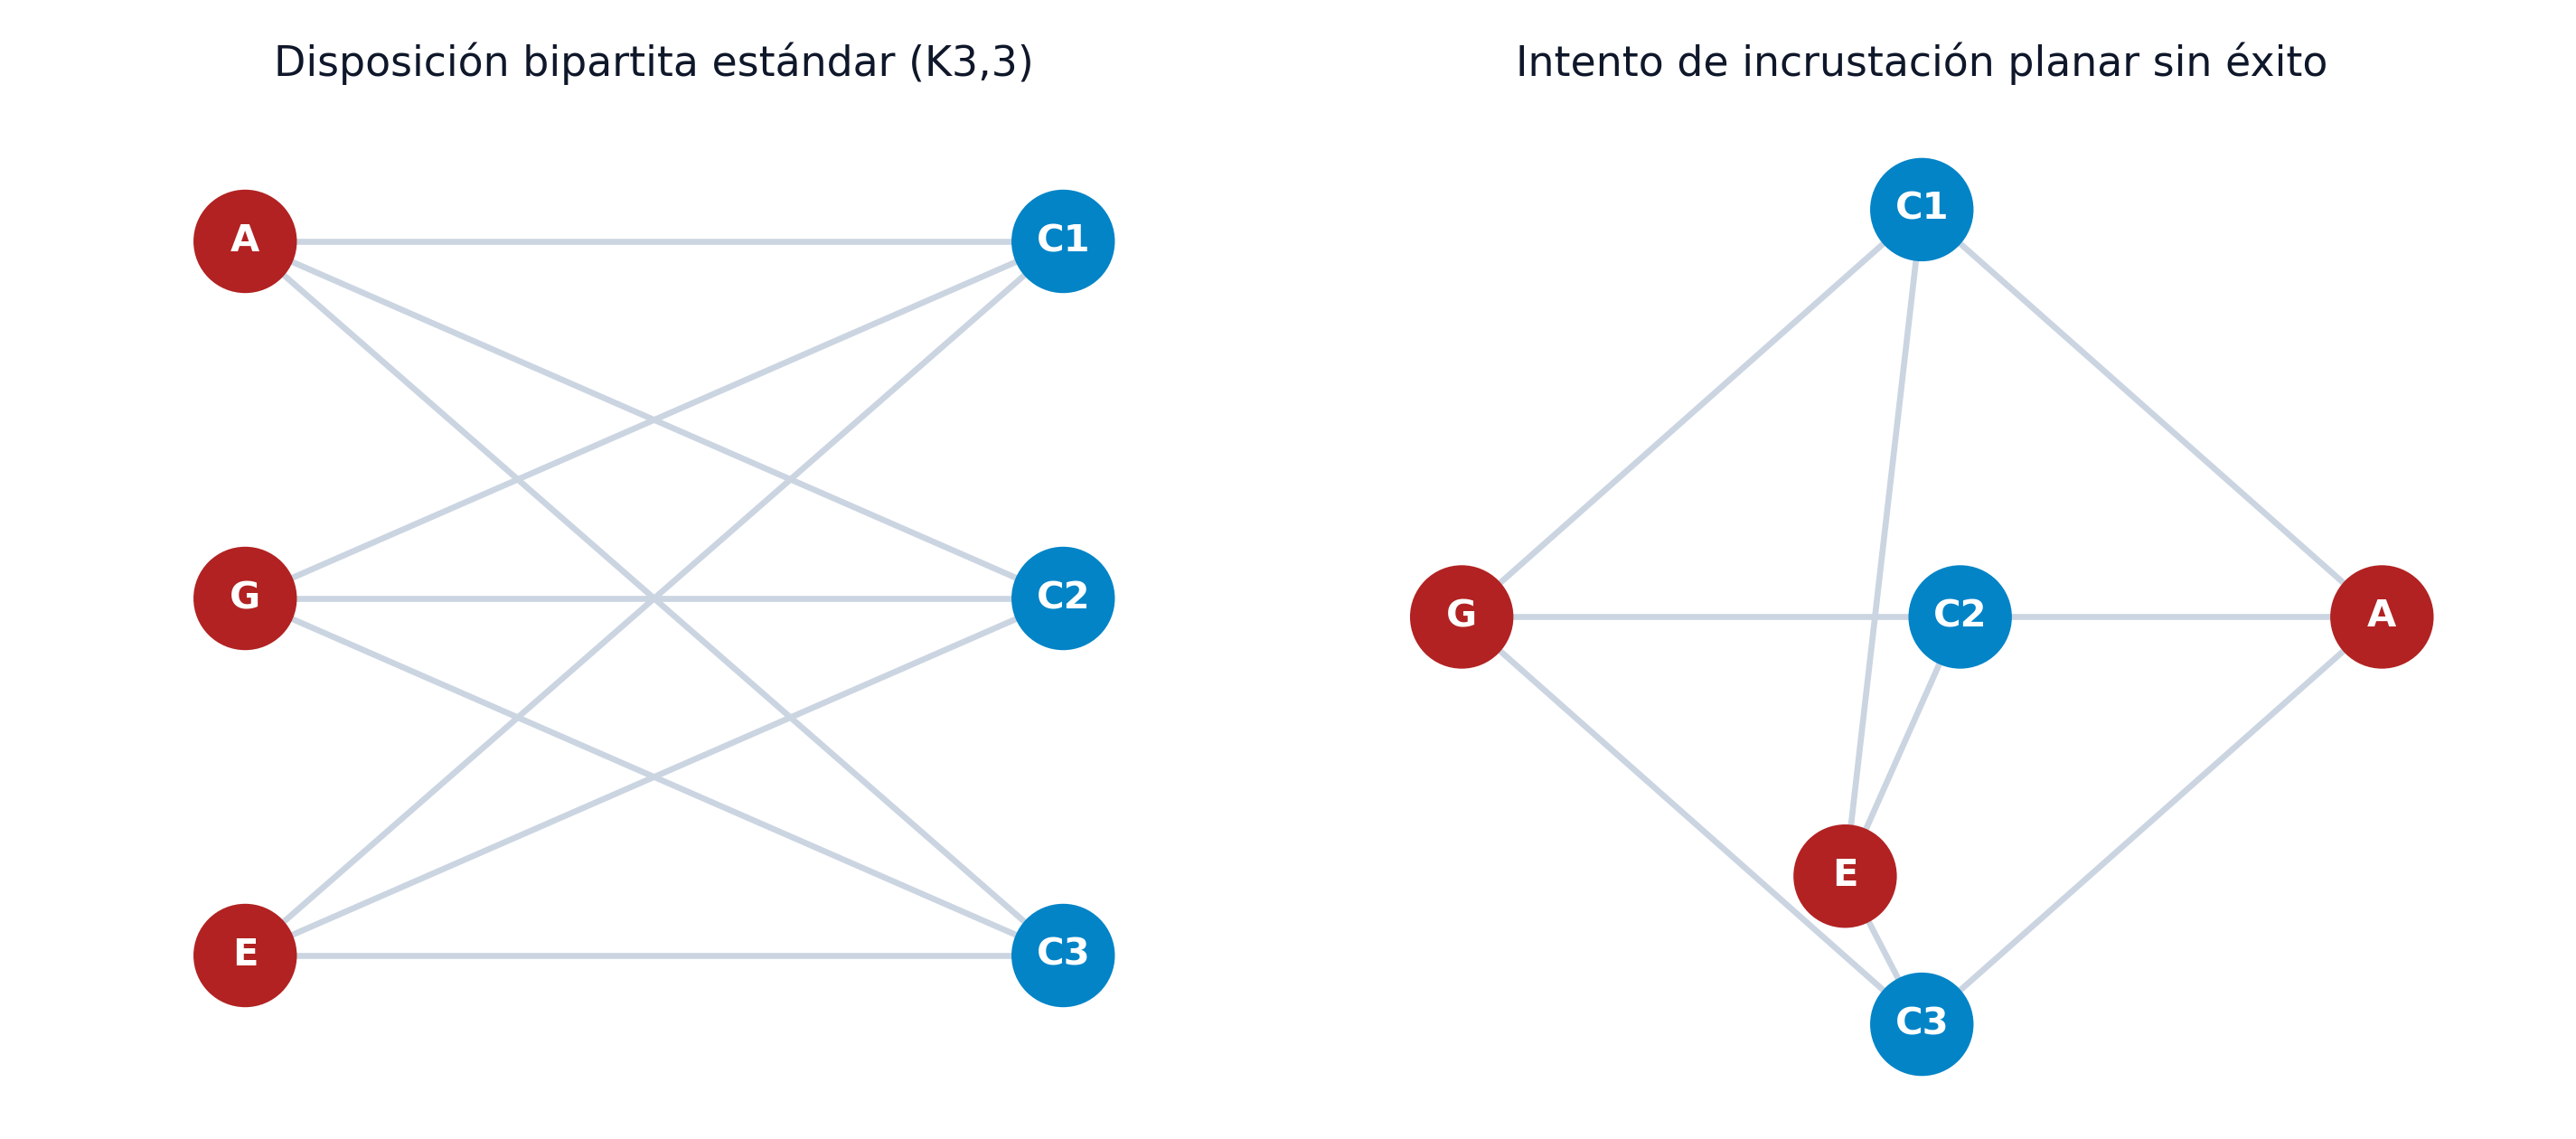
\includegraphics[width=0.85\linewidth,height=\textheight,keepaspectratio]{images/k33_bipartito_dudeney.png}

}

\caption{\label{fig-k33-bipartito}Problema de los tres servicios de
Dudeney e imposibilidad de incrustación planar de K3,3}

\end{figure}%

Los grafos \(K_5\) y \(K_{3,3}\) representan las dos estructuras
elementales ``obstructoras'' que impiden que una red pueda ser dibujada
en el plano. Para caracterizar la planaridad en grafos arbitrarios de
mayor escala, se introduce el concepto de \textbf{homeomorfismo}.

\begin{tcolorbox}[enhanced jigsaw, toprule=.15mm, opacitybacktitle=0.6, coltitle=black, colbacktitle=quarto-callout-note-color!10!white, title=\textcolor{quarto-callout-note-color}{\faInfo}\hspace{0.5em}{Definición: Grafos homeomórficos}, arc=.35mm, rightrule=.15mm, toptitle=1mm, breakable, bottomtitle=1mm, titlerule=0mm, colback=white, opacityback=0, leftrule=.75mm, colframe=quarto-callout-note-color-frame, left=2mm, bottomrule=.15mm]

Dos grafos \(G_1\) y \(G_2\) se dicen \textbf{homeomórficos} (o
homeomorfos) si uno de ellos puede obtenerse a partir del otro mediante
una secuencia finita de operaciones de \textbf{subdivisión elemental de
aristas} (insertar un nodo de grado 2 en medio de una arista) o de
suprimir vértices de grado 2.

\end{tcolorbox}

En 1930, el matemático polaco Kazimierz Kuratowski formuló la
caracterización definitiva que resuelve el problema de la planaridad en
la teoría de grafos.

\begin{tcolorbox}[enhanced jigsaw, toprule=.15mm, opacitybacktitle=0.6, coltitle=black, colbacktitle=quarto-callout-important-color!10!white, title=\textcolor{quarto-callout-important-color}{\faExclamation}\hspace{0.5em}{Teorema: Teorema de Kuratowski (1930)}, arc=.35mm, rightrule=.15mm, toptitle=1mm, breakable, bottomtitle=1mm, titlerule=0mm, colback=white, opacityback=0, leftrule=.75mm, colframe=quarto-callout-important-color-frame, left=2mm, bottomrule=.15mm]

Un grafo \(G = (V, E)\) es \textbf{planar} si y solo si no contiene
ningún subgrafo parcial que sea \textbf{homeomórfico} a \(K_5\) ó a
\(K_{3,3}\): \[
G \text{ es no planar} \iff \exists H \subseteq G \text{ tal que } H \text{ es homeomorfo a } K_5 \text{ ó } K_{3,3}
\]

\end{tcolorbox}

\begin{figure}

\centering{

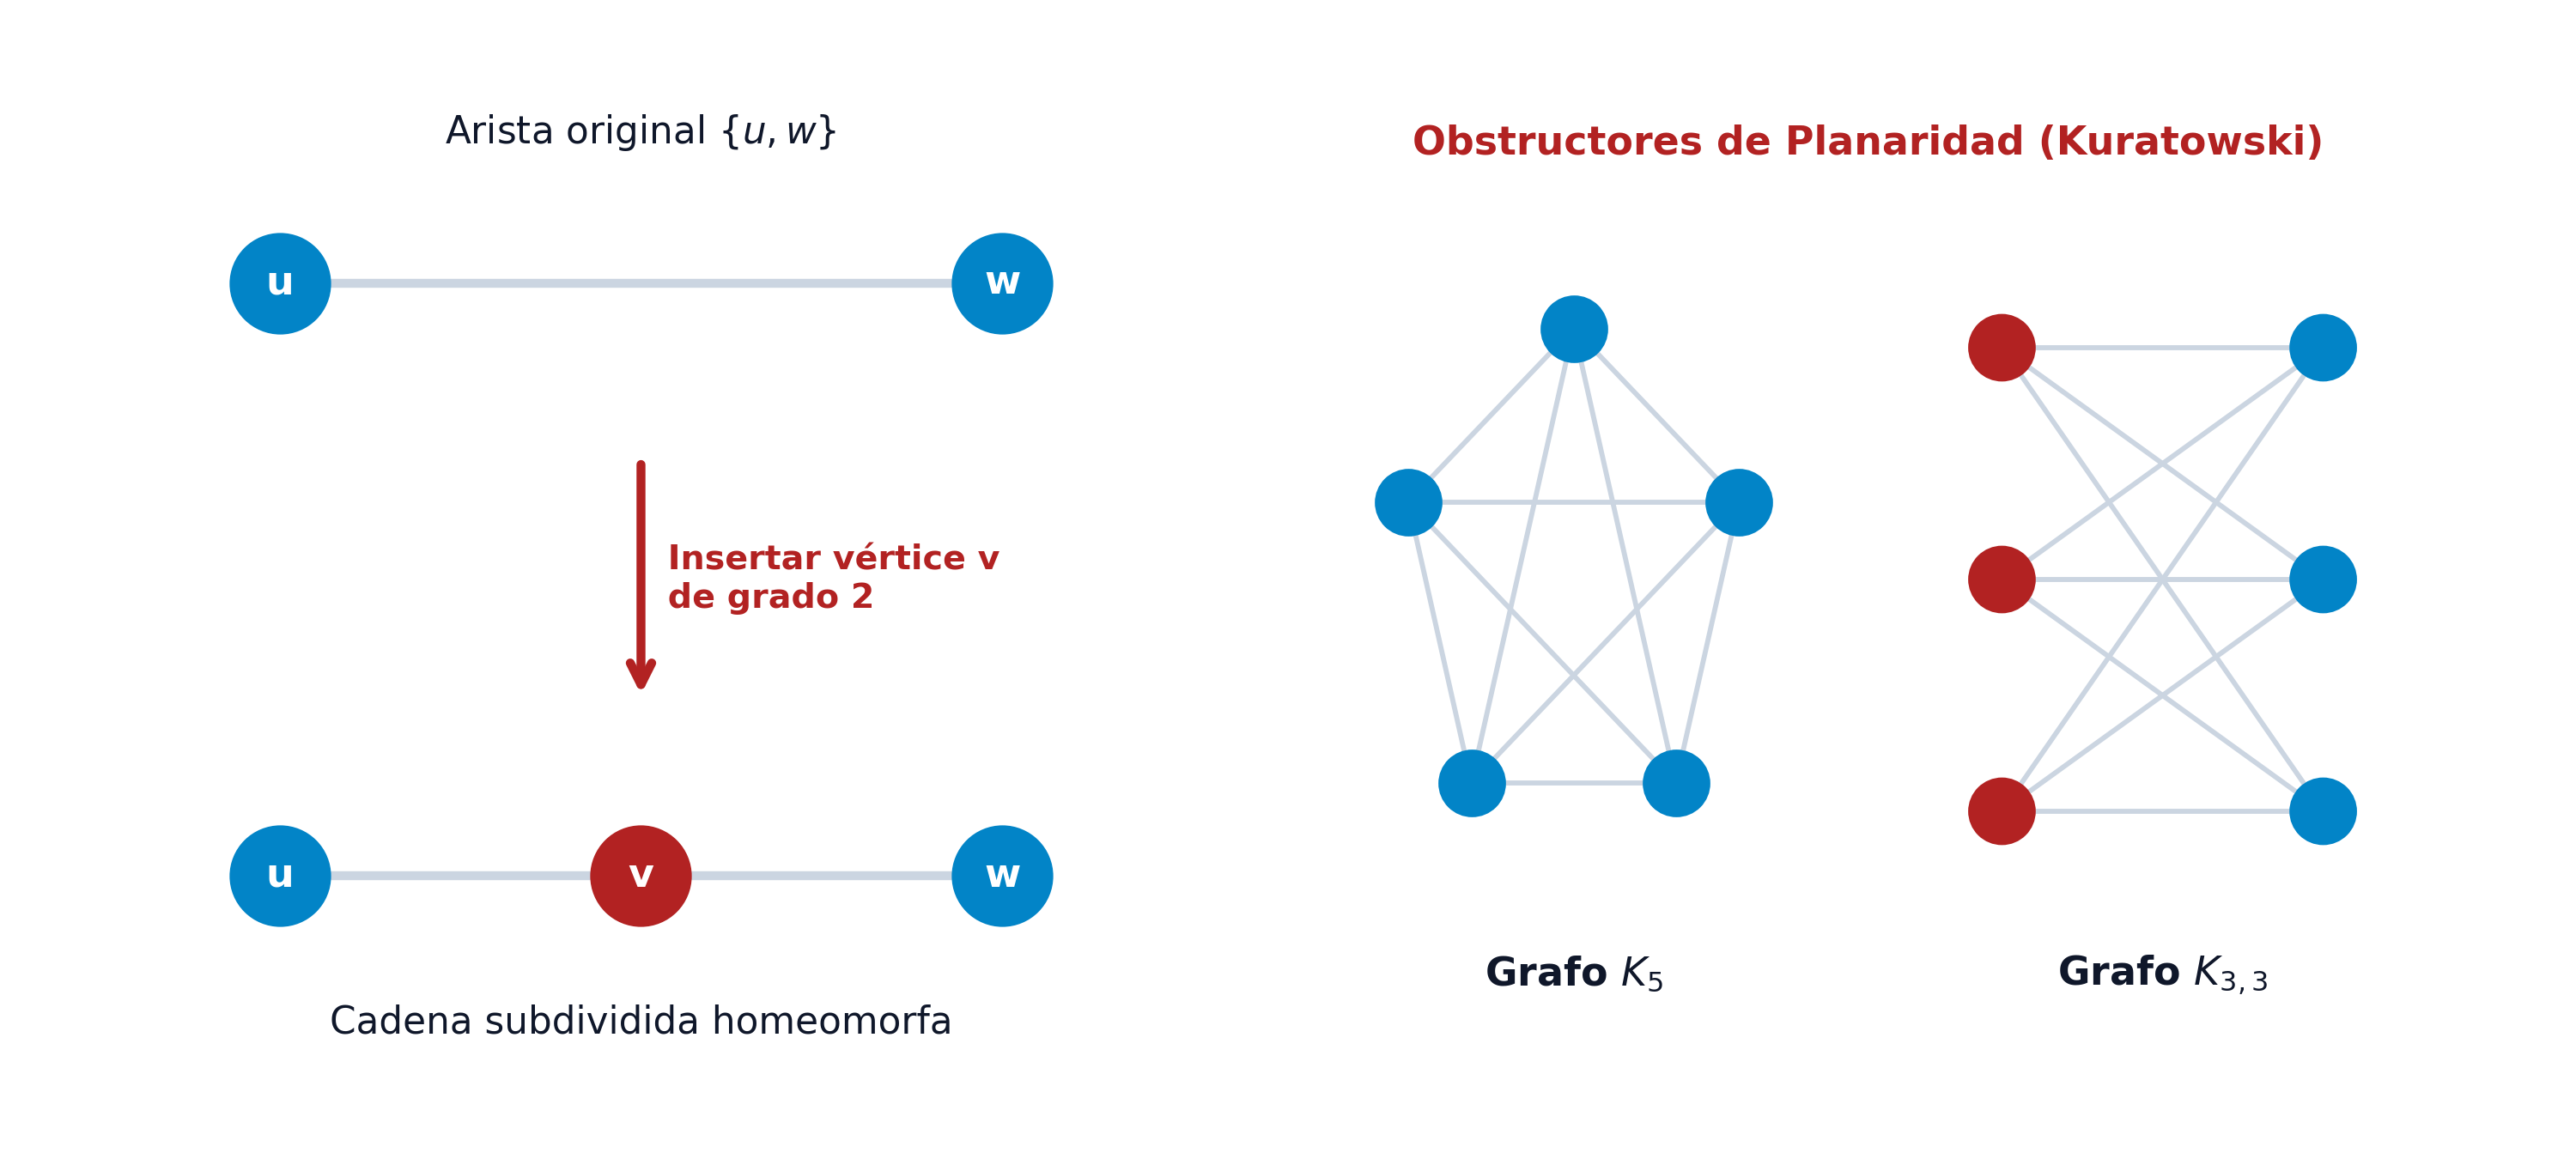
\includegraphics[width=0.85\linewidth,height=\textheight,keepaspectratio]{images/kuratowski_homeomorfismo.png}

}

\caption{\label{fig-kuratowski-homeomorfismo}Subdivisión elemental de
aristas y caracterización de Kuratowski mediante K5 y K3,3}

\end{figure}%

Un caso emblemático de aplicación del Teorema de Kuratowski lo
constituye el \textbf{Grafo de Petersen}, un grafo 3-regular formado por
10 vértices y 15 aristas (integrado por una estrella pentagonal interior
inscrita en un pentágono exterior).

\begin{tcolorbox}[enhanced jigsaw, toprule=.15mm, opacitybacktitle=0.6, coltitle=black, colbacktitle=quarto-callout-note-color!10!white, title=\textcolor{quarto-callout-note-color}{\faInfo}\hspace{0.5em}{Definición: Grafo de Petersen y sus propiedades}, arc=.35mm, rightrule=.15mm, toptitle=1mm, breakable, bottomtitle=1mm, titlerule=0mm, colback=white, opacityback=0, leftrule=.75mm, colframe=quarto-callout-note-color-frame, left=2mm, bottomrule=.15mm]

El \textbf{Grafo de Petersen} es un grafo 3-regular (todos sus vértices
poseen grado exactamente \(\delta(v) = 3\)) que satisface las siguientes
propiedades combinatorias únicas:

\begin{itemize}
\item
  Dos vértices adyacentes cualesquiera no comparten ningún vecino en
  común.
\item
  Dos vértices no adyacentes cualesquiera comparten exactamente un
  vecino en común.
\end{itemize}

\end{tcolorbox}

Como se ilustra en la Figura~\ref{fig-petersen-homeomorfismo}, a pesar
de su elevada simetría geométrica, el \textbf{Grafo de Petersen es no
planar}. La demostración formal se obtiene aplicando el Criterio de
Kuratowski mediante la identificación de un subgrafo parcial
homeomórfico al grafo bipartito completo \(K_{3,3}\):

\begin{figure}

\centering{

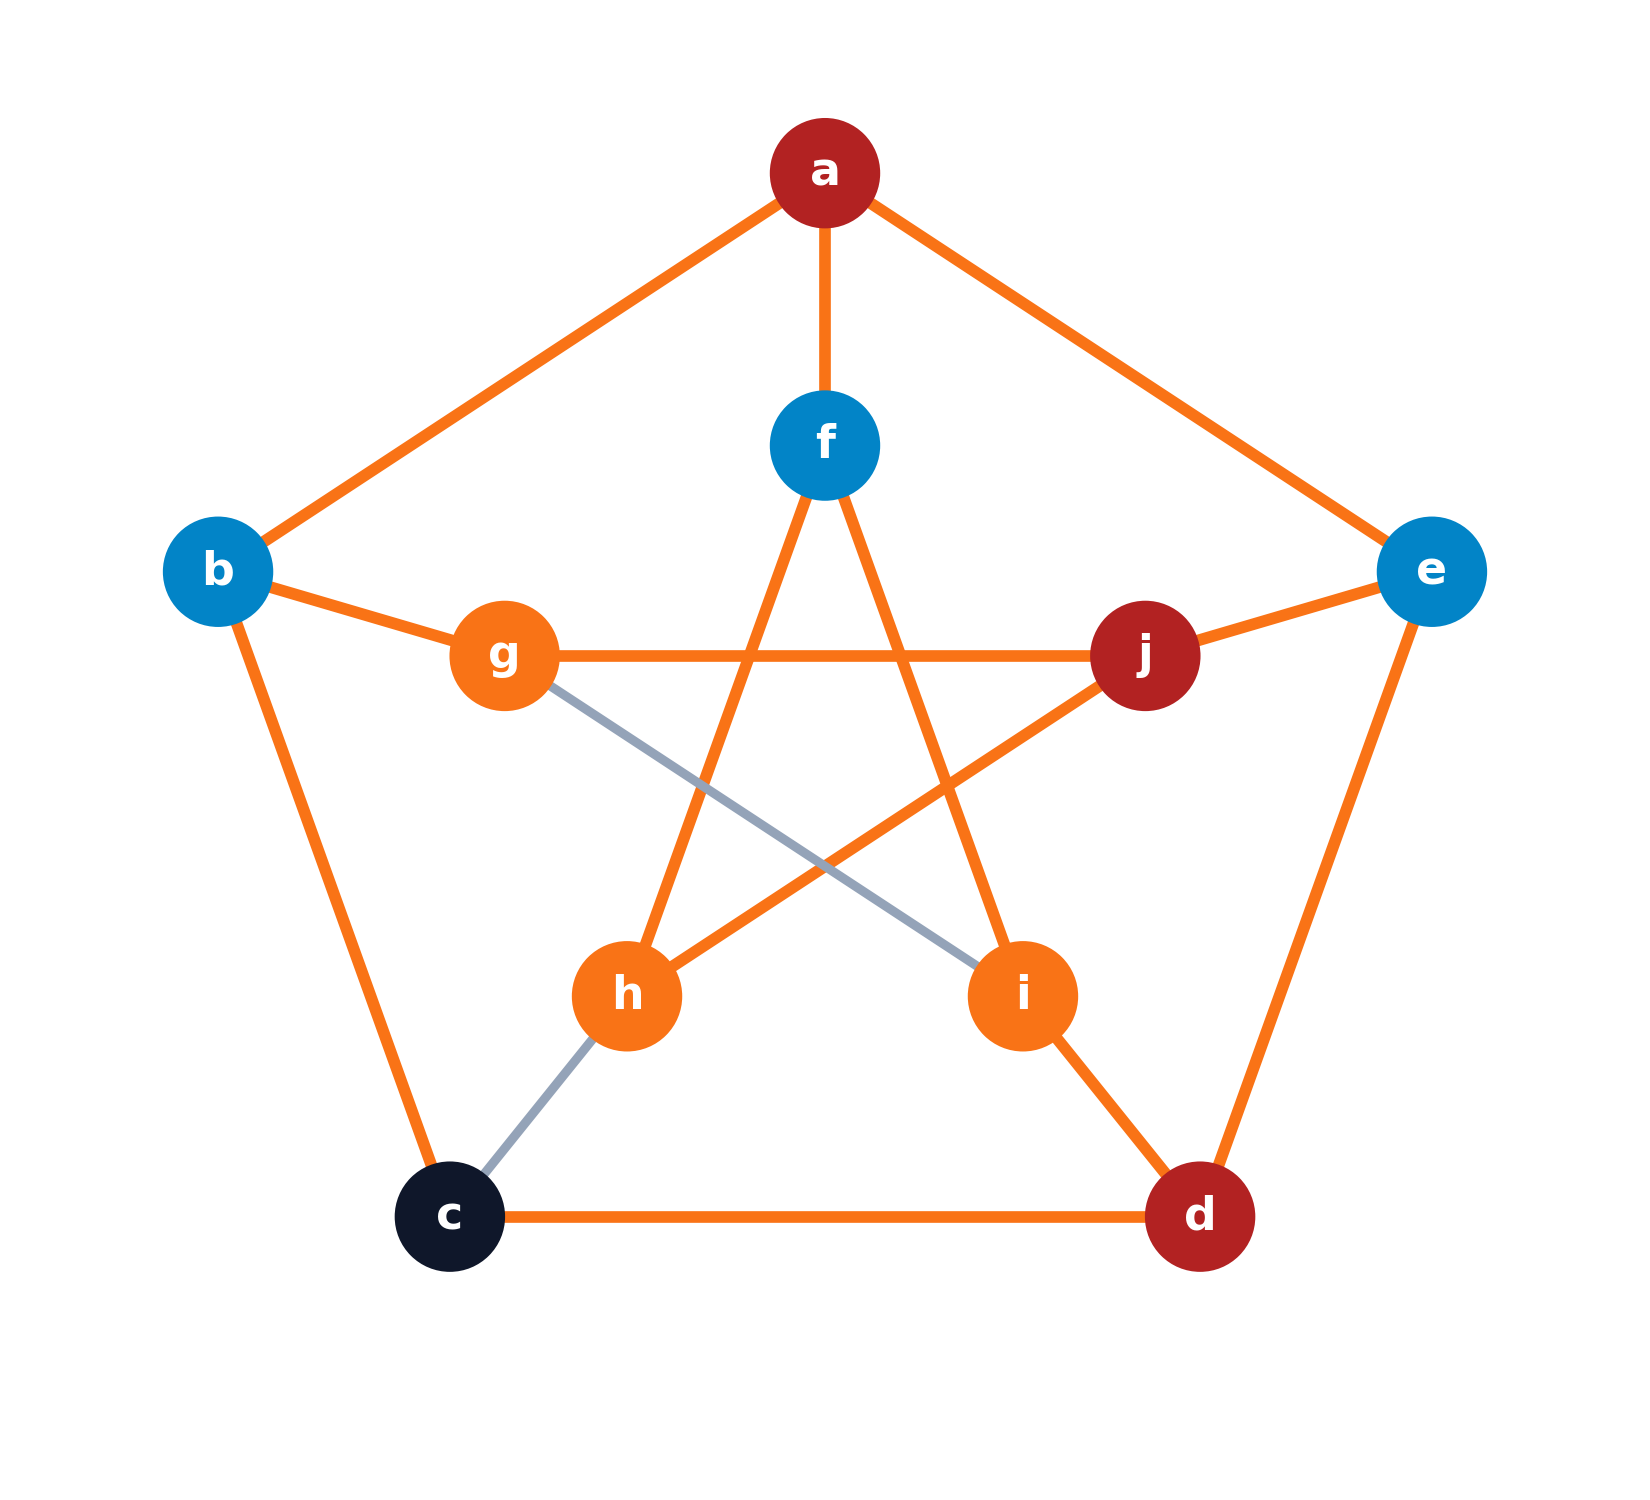
\includegraphics[width=0.55\linewidth,height=\textheight,keepaspectratio]{images/petersen_k33_homeomorfismo.png}

}

\caption{\label{fig-petersen-homeomorfismo}Demostración de no planaridad
del Grafo de Petersen mediante homeomorfismo a K3,3}

\end{figure}%

Para comprender cómo se manifiesta el obstructo de Kuratowski en esta
estructura, se analizan los roles que desempeñan sus nodos y aristas:

\begin{enumerate}
\def\labelenumi{\arabic{enumi}.}
\item
  \textbf{Partición de Vértices del Bipartito \(K_{3,3}\)}:
  Seleccionamos los subconjuntos disjuntos \(V_1 = \{j, a, d\}\) (nodos
  rojos) y \(V_2 = \{e, f, b\}\) (nodos azules).
\item
  \textbf{Construcción de las 9 Cadenas Independientes}: Para verificar
  la estructura de \(K_{3,3}\), cada uno de los 3 vértices de \(V_1\)
  debe estar comunicado con los 3 vértices de \(V_2\) mediante cadenas
  disjuntas en sus aristas interiores (resaltadas en color naranja):

  \begin{itemize}
  \tightlist
  \item
    \textbf{Conexiones desde \(a \in V_1\)}: El nodo \(a\) conecta
    directamente con \(b, e, f \in V_2\) mediante las 3 aristas
    adyacentes \(\{a,b\}\), \(\{a,e\}\) y \(\{a,f\}\).
  \item
    \textbf{Conexiones desde \(j \in V_1\)}: El nodo \(j\) conecta
    directamente con \(e \in V_2\) (\(\{j,e\}\)); se comunica con
    \(f \in V_2\) mediante la cadena \(j \to h \to f\) (usando el nodo
    intermedio \(h\) de grado 2); y se comunica con \(b \in V_2\)
    mediante la cadena \(j \to g \to b\) (usando el nodo intermedio
    \(g\)).
  \item
    \textbf{Conexiones desde \(d \in V_1\)}: El nodo \(d\) conecta
    directamente con \(e \in V_2\) (\(\{d,e\}\)); se comunica con
    \(b \in V_2\) mediante la cadena \(d \to c \to b\) (usando el nodo
    intermedio \(c\)); y se comunica con \(f \in V_2\) mediante la
    cadena \(d \to i \to f\) (usando el nodo intermedio \(i\)).
  \end{itemize}
\item
  \textbf{Aristas Excluidas (en gris)}: Las aristas \(\{g, i\}\) y
  \(\{c, h\}\) (representadas en gris en la
  Figura~\ref{fig-petersen-homeomorfismo}) no se utilizan para conformar
  el subgrafo y se suprimen.
\end{enumerate}

Dado que todos los vértices intermedios (\(g, h, i, c\)) actúan como
nodos de grado 2 que subdividen aristas, el subgrafo parcial resultante
es \textbf{homeomórfico a \(K_{3,3}\)}, lo que prueba de forma
concluyente que el Grafo de Petersen \textbf{no admite incrustación
planar}.

A partir de la caracterización de Kuratowski, se observa intuitivamente
que un grafo con una alta densidad de aristas resulta progresivamente
más difícil de incrustar en el plano sin provocar intersecciones. Esta
relación cuantitativa entre la densidad de aristas y la topología planar
fue formalizada originalmente por Leonhard Euler al vincular el número
de vértices (\(n\)), el número de aristas (\(m\)) y el número de caras o
regiones (\(r\)) que delimita el grafo sobre el plano bidimensional.

\begin{tcolorbox}[enhanced jigsaw, toprule=.15mm, opacitybacktitle=0.6, coltitle=black, colbacktitle=quarto-callout-important-color!10!white, title=\textcolor{quarto-callout-important-color}{\faExclamation}\hspace{0.5em}{Teorema: Fórmula planar de Euler}, arc=.35mm, rightrule=.15mm, toptitle=1mm, breakable, bottomtitle=1mm, titlerule=0mm, colback=white, opacityback=0, leftrule=.75mm, colframe=quarto-callout-important-color-frame, left=2mm, bottomrule=.15mm]

Sea \(G = (V, E)\) un grafo planar conexo con \(n = |V|\) vértices y
\(m = |E|\) aristas. Si \(r\) denota el número de regiones delimitadas
en cualquier incrustación planar de \(G\) (incluyendo la región exterior
no acotada), entonces se verifica exactamente la relación: \[
n + r = m + 2
\]

\emph{Demostración}: Realizaremos la demostración por inducción
matemática sobre el número de aristas \(m \ge 0\).

\begin{itemize}
\item
  \textbf{Base Inductiva (\(m = 0\))}: Si \(m = 0\), al ser \(G\)
  conexo, el grafo consta de un único vértice aislado (\(n = 1\)). El
  número de regiones en el plano es la única región exterior no acotada
  (\(r = 1\)). Sustituyendo: \[
  n + r = 1 + 1 = 2 = 0 + 2 = m + 2
  \] Se cumple la igualdad base.
\item
  \textbf{Paso Inductivo}: Asumimos como hipótesis de inducción que la
  relación \(n' + r' = m' + 2\) es válida para todo grafo planar conexo
  con \(m' = m - 1\) aristas. Consideremos ahora un grafo planar conexo
  \(G\) con \(m\) aristas:

  \begin{itemize}
  \item
    \textbf{Caso 1 (G es un árbol)}: Si \(G\) no contiene ningún ciclo,
    entonces es un árbol y posee exactamente \(m = n - 1\) aristas. Como
    no encierra ningún ciclo, la única cara existente es la región
    exterior (\(r = 1\)). Reemplazando: \[
    n + r = n + 1 = (m + 1) + 1 = m + 2
    \] Queda verificado.
  \item
    \textbf{Caso 2 (G contiene al menos un ciclo)}: Si \(G\) contiene al
    menos un ciclo, seleccionamos una arista \(e \in E\) que pertenezca
    a dicho ciclo. Al eliminar la arista \(e\), obtenemos un subgrafo
    parcial \(G' = (V, E \setminus \{e\})\) que sigue siendo conexo, con
    \(n' = n\) vértices y \(m' = m - 1\) aristas. Dado que la arista
    \(e\) actuaba como frontera común separando dos regiones contiguas
    de \(G\), su eliminación destruye dicha frontera y fusiona las dos
    regiones en una sola, por lo que \(r' = r - 1\). Por hipótesis
    inductiva aplicada a \(G'\): \[
    n' + r' = m' + 2 \implies n + (r - 1) = (m - 1) + 2 \implies n + r = m + 2
    \]
  \end{itemize}
\end{itemize}

Por el principio de inducción matemática, el teorema queda rigurosamente
demostrado para todo grafo planar conexo. \(\blacksquare\)

\end{tcolorbox}

La Fórmula de Euler permite establecer cotas superiores algebraicas
estrictas sobre el número máximo de aristas que puede contener un grafo
antes de perder la propiedad de ser planar.

\begin{tcolorbox}[enhanced jigsaw, toprule=.15mm, opacitybacktitle=0.6, coltitle=black, colbacktitle=quarto-callout-note-color!10!white, title=\textcolor{quarto-callout-note-color}{\faInfo}\hspace{0.5em}{Corolario: Desigualdades de planaridad y condición necesaria}, arc=.35mm, rightrule=.15mm, toptitle=1mm, breakable, bottomtitle=1mm, titlerule=0mm, colback=white, opacityback=0, leftrule=.75mm, colframe=quarto-callout-note-color-frame, left=2mm, bottomrule=.15mm]

\begin{enumerate}
\def\labelenumi{\arabic{enumi}.}
\item
  En todo grafo planar conexo simple \(G\) con \(n \ge 3\) vértices y
  \(m\) aristas:

  \[
  m \le 3n - 6
  \]
\item
  En todo grafo planar conexo simple \textbf{bipartito} (sin triángulos,
  donde la longitud de todo ciclo es \(\ge 4\)) con \(n \ge 3\): \[
  m \le 2n - 4
  \]
\end{enumerate}

\emph{Demostración}: En un grafo simple conexo, cada región \(i\) está
delimitada por al menos 3 aristas. Al sumar las aristas frontera de
todas las \(r\) regiones, cada arista es compartida como máximo por 2
regiones: \[
3r \le \sum_{i=1}^r \text{aristas}(r_i) = 2m \implies r \le \frac{2}{3}m
\] Sustituyendo \(r \le \frac{2}{3}m\) en la fórmula de Euler
\(n + r = m + 2\): \[
n + \frac{2}{3}m \ge m + 2 \implies n - 2 \ge \frac{1}{3}m \implies m \le 3n - 6 \quad \blacksquare
\]

\end{tcolorbox}

\begin{tcolorbox}[enhanced jigsaw, toprule=.15mm, opacitybacktitle=0.6, coltitle=black, colbacktitle=quarto-callout-tip-color!10!white, title=\textcolor{quarto-callout-tip-color}{\faLightbulb}\hspace{0.5em}{Ejemplo: Demostración analítica de no planaridad}, arc=.35mm, rightrule=.15mm, toptitle=1mm, breakable, bottomtitle=1mm, titlerule=0mm, colback=white, opacityback=0, leftrule=.75mm, colframe=quarto-callout-tip-color-frame, left=2mm, bottomrule=.15mm]

\textbf{Demostrar analíticamente que los grafos \(K_5\) (completo de 5
vértices) y \(K_{3,3}\) (bipartito completo de los 3 suministros) no son
planares.}

\textbf{Resolución para \(K_5\)} El grafo completo \(K_5\) posee
\(n = 5\) vértices y \(m = \binom{5}{2} = 10\) aristas. Si \(K_5\) fuera
planar, debería verificar la desigualdad \(m \le 3n - 6\): \[
10 \le 3(5) - 6 = 15 - 6 = 9 \quad \text{(FALSO)}
\] Dado que \(10 \le 9\) es falso, \(K_5\) es \textbf{no planar}.

\textbf{Resolución para \(K_{3,3}\) (Problema de Dudeney)} El grafo
bipartito de Dudeney \(K_{3,3}\) posee \(n = 6\) vértices y
\(m = 3 \times 3 = 9\) aristas, sin ningún triángulo interno. Si fuera
planar, debería cumplir \(m \le 2n - 4\): \[
9 \le 2(6) - 4 = 12 - 4 = 8 \quad \text{(FALSO)}
\] Dado que \(9 \le 8\) es falso, \(K_{3,3}\) es \textbf{no planar}.

\end{tcolorbox}

\begin{center}\rule{0.5\linewidth}{0.5pt}\end{center}

\section{Representación de grafos}\label{representaciuxf3n-de-grafos}

Para almacenar, manipular y ejecutar algoritmos de optimización sobre
redes mediante ordenadores, la topología de un grafo o digrafo debe
traducirse a estructuras de datos computacionales eficientes. Atendiendo
a la densidad de aristas, a la variabilidad temporal de la red y a las
operaciones algorítmicas requeridas, la teoría de grafos ofrece tres
modalidades fundamentales de representación: matricial, vectorial y por
listas de adyacencia.

\subsection{Representación matricial}\label{representaciuxf3n-matricial}

Para procesar, analizar y resolver problemas de optimización sobre redes
mediante ordenadores, la topología de un grafo o digrafo debe
codificarse de forma algebraica. Las dos formas matriciales clásicas
para representar las conexiones de una red son la \textbf{matriz de
incidencia} y la \textbf{matriz de adyacencia}.

\begin{tcolorbox}[enhanced jigsaw, toprule=.15mm, opacitybacktitle=0.6, coltitle=black, colbacktitle=quarto-callout-note-color!10!white, title=\textcolor{quarto-callout-note-color}{\faInfo}\hspace{0.5em}{Definición: Matriz de incidencia de un grafo no dirigido}, arc=.35mm, rightrule=.15mm, toptitle=1mm, breakable, bottomtitle=1mm, titlerule=0mm, colback=white, opacityback=0, leftrule=.75mm, colframe=quarto-callout-note-color-frame, left=2mm, bottomrule=.15mm]

Dado un grafo no dirigido \(G = (V, E)\) con \(n = |V|\) vértices
(\(V = \{1, \dots, n\}\)) y \(m = |E|\) aristas
(\(E = \{e_1, \dots, e_m\}\)), la \textbf{matriz de incidencia
nodo-arista} es una matriz rectangular
\(A = (a_{ik}) \in \mathbb{R}^{n \times m}\) definida por: \[
a_{ik} = \begin{cases}
1 & \text{si } e_k = \{i, *\} \in E \text{ (el nodo } i \text{ es uno de los dos extremos de la arista } e_k\text{)}, \\
0 & \text{en otro caso.}
\end{cases}
\]

\end{tcolorbox}

En un grafo no dirigido, cada columna de la matriz de incidencia \(A\)
contiene exactamente dos unos, correspondientes a los dos nodos que une
la arista respectiva. Asimismo, la suma de los elementos de la fila
\(i\)-ésima coincide exactamente con el grado del nodo, es decir,
\(\sum_{k=1}^m a_{ik} = d(i)\). En la
Figura~\ref{fig-matriz-incidencia-grafo} se ilustra la construcción
explícita de esta matriz para un grafo no dirigido sobre 4 vértices y 5
aristas.

\begin{figure}

\centering{

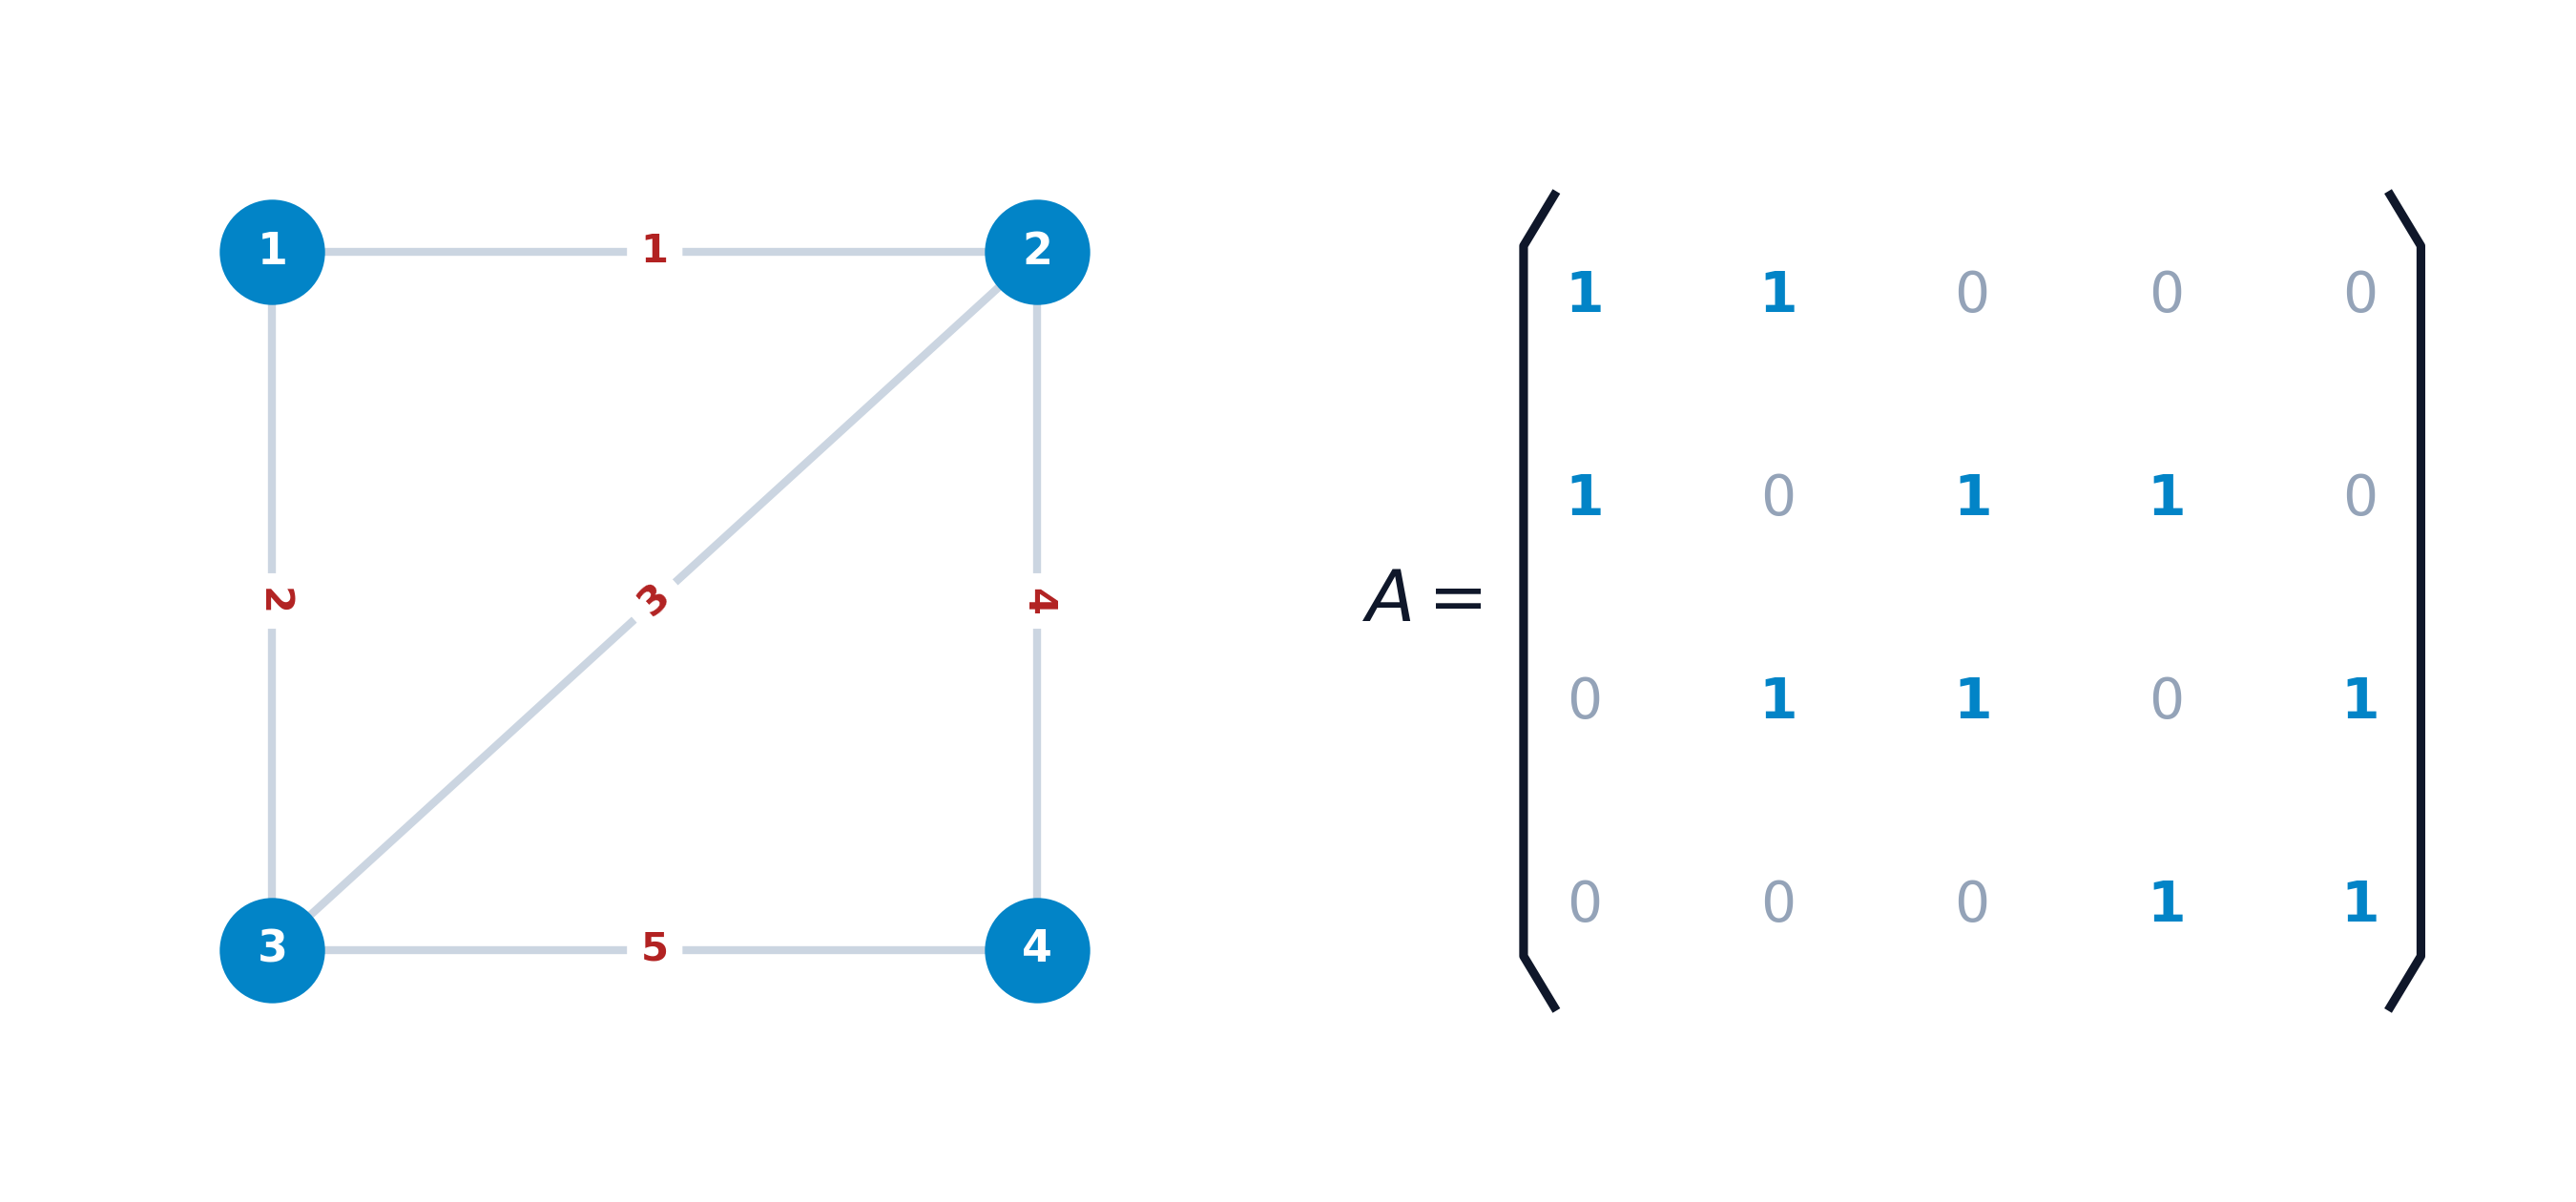
\includegraphics[width=0.8\linewidth,height=\textheight,keepaspectratio]{images/matriz_incidencia_grafo.png}

}

\caption{\label{fig-matriz-incidencia-grafo}Grafo no dirigido de muestra
y su correspondiente matriz de incidencia nodo-arista A}

\end{figure}%

Cuando la red posee orientación en sus conexiones, la matriz de
incidencia incorpora el signo de la dirección del flujo de cada arco.

\begin{tcolorbox}[enhanced jigsaw, toprule=.15mm, opacitybacktitle=0.6, coltitle=black, colbacktitle=quarto-callout-note-color!10!white, title=\textcolor{quarto-callout-note-color}{\faInfo}\hspace{0.5em}{Definición: Matriz de incidencia de un digrafo}, arc=.35mm, rightrule=.15mm, toptitle=1mm, breakable, bottomtitle=1mm, titlerule=0mm, colback=white, opacityback=0, leftrule=.75mm, colframe=quarto-callout-note-color-frame, left=2mm, bottomrule=.15mm]

Dado un digrafo \(G = (V, U)\) con \(n = |V|\) vértices y \(m = |U|\)
arcos dirigidos (\(U = \{u_1, \dots, u_m\}\)), la \textbf{matriz de
incidencia nodo-arco} es una matriz rectangular
\(A = (a_{ik}) \in \mathbb{R}^{n \times m}\) definida por: \[
a_{ik} = \begin{cases}
1 & \text{si } u_k = (i, *) \in U \text{ (el arco } u_k \text{ parte del nodo } i\text{)}, \\
-1 & \text{si } u_k = (*, i) \in U \text{ (el arco } u_k \text{ llega al nodo } i\text{)}, \\
0 & \text{en otro caso.}
\end{cases}
\]

\end{tcolorbox}

En esta formulación, cada columna \(k = (i, j)\) de la matriz de
incidencia de un digrafo contiene exactamente un \(+1\) en la fila del
nodo de origen \(i\) y un \(-1\) en la fila del nodo de destino \(j\) (o
viceversa según el convenio algebraico fijado). Como consecuencia, la
suma de todos los elementos de cada columna es nula
(\(\sum_{i=1}^n a_{ik} = 0\)), lo que implica que el rango de la matriz
para un digrafo conexo de \(n\) vértices es a lo sumo
\(\text{rango}(A) = n - 1\). Esta propiedad confiere a la matriz de
incidencia de digrafos la característica de \textbf{Total Unimodularidad
(TUM)}, fundamental en programación lineal entera para garantizar que
los problemas de flujo balanceado \(A x = b\) con datos enteros admitan
siempre soluciones óptimas enteras sin necesidad de algoritmos de
ramificación. En la Figura~\ref{fig-matriz-incidencia-digrafo} se
presenta la matriz de incidencia resultante para un digrafo dirigido
sobre 4 vértices.

\begin{figure}

\centering{

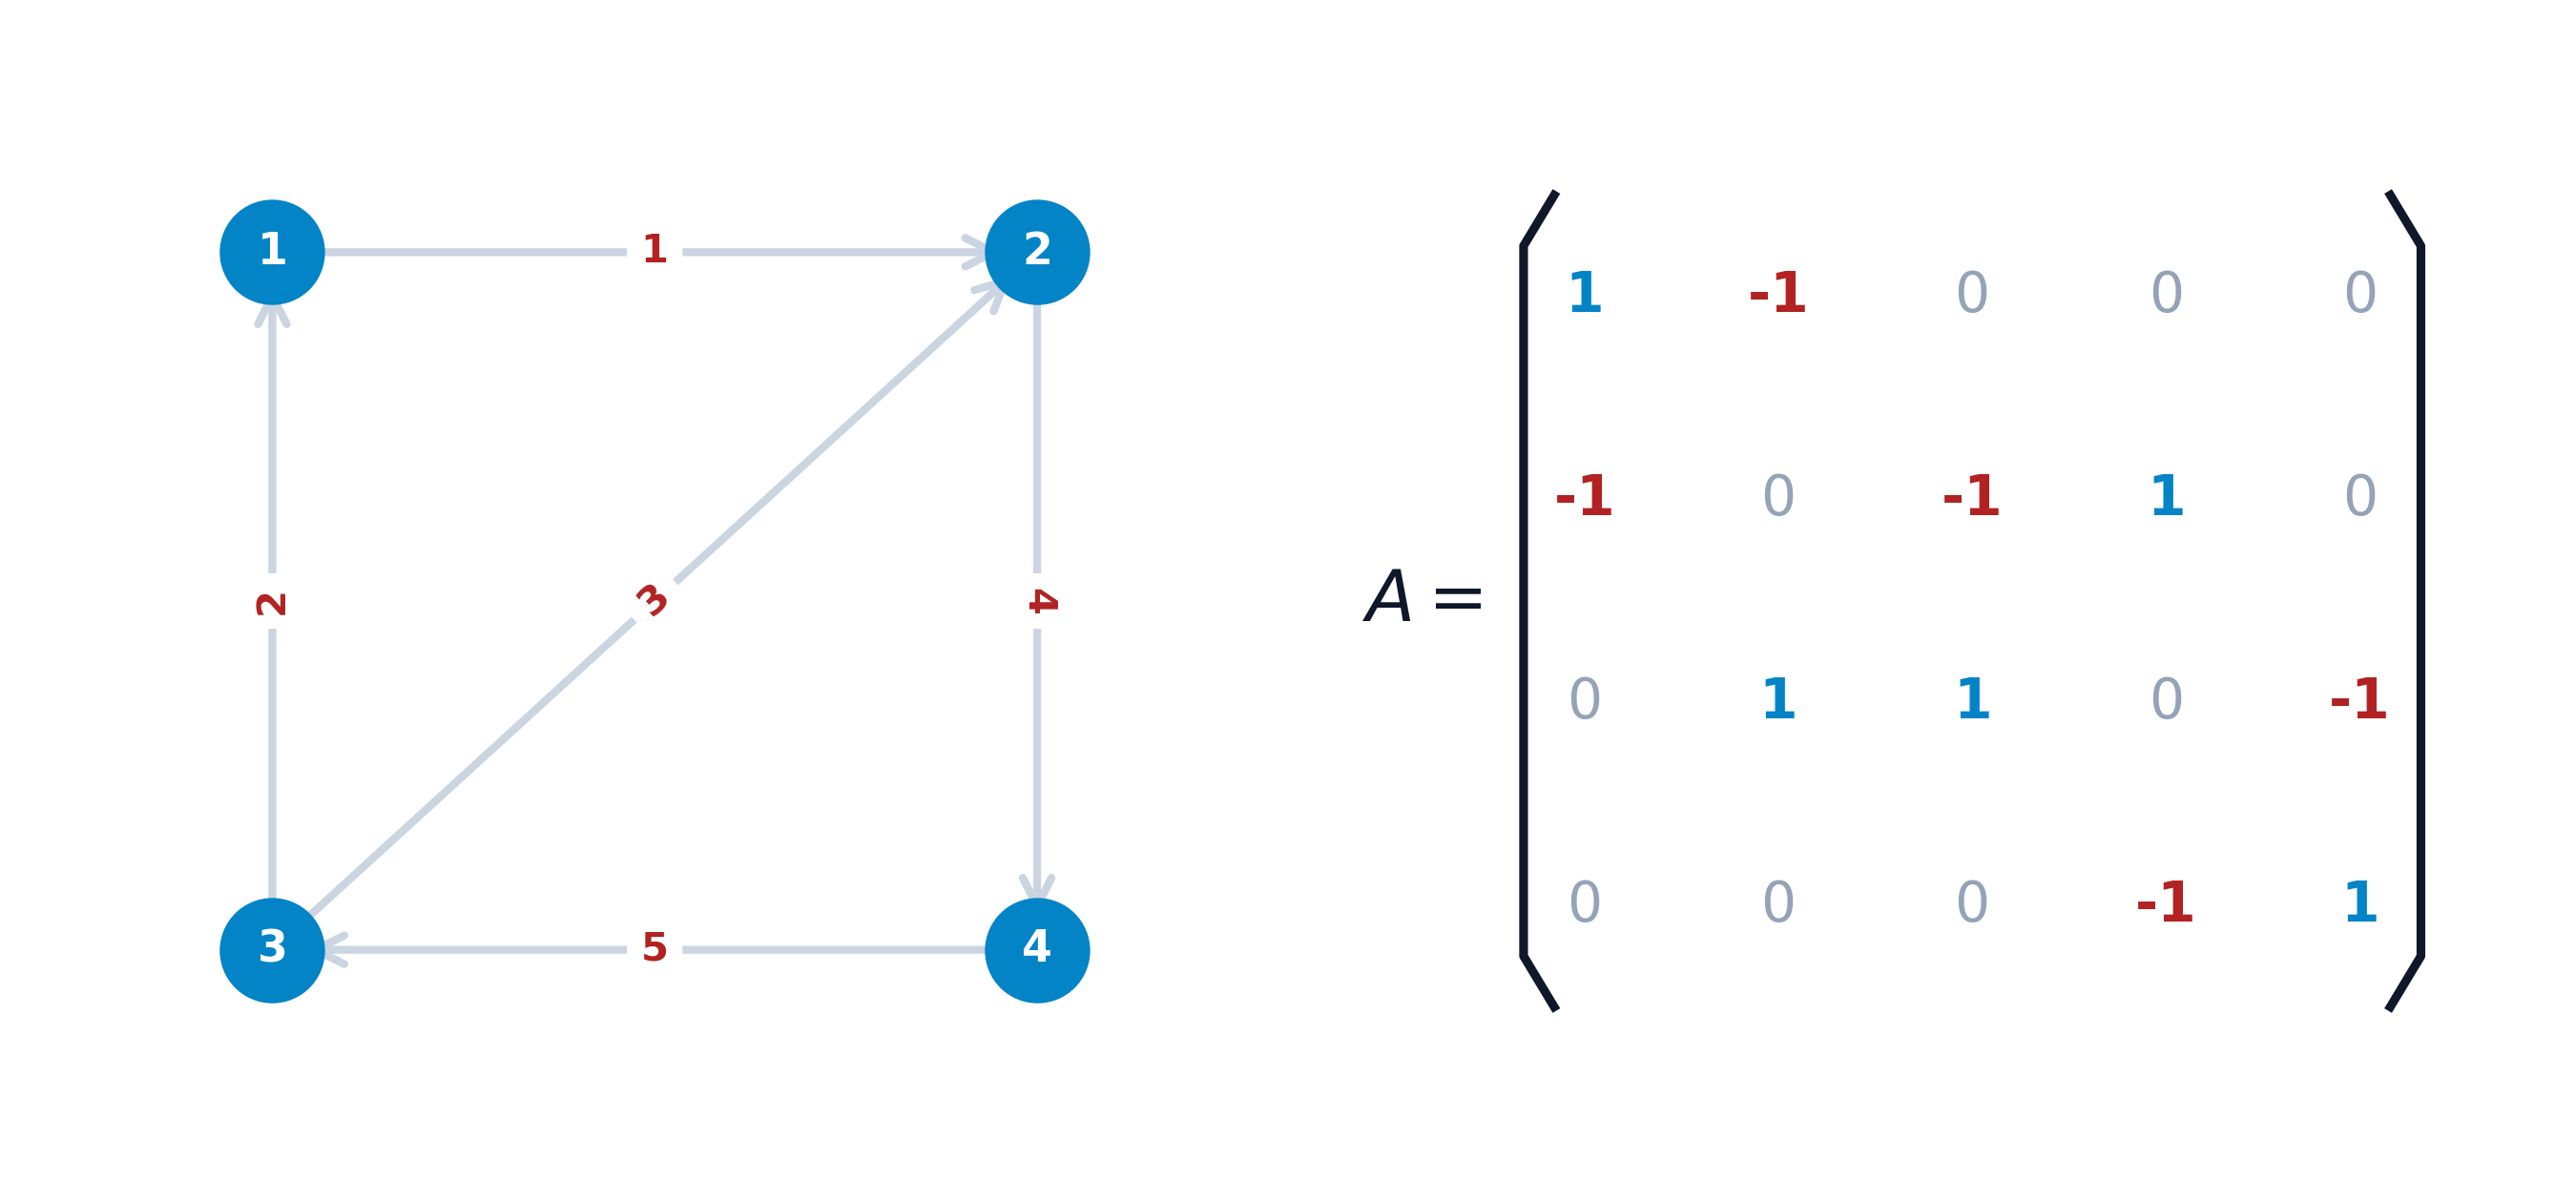
\includegraphics[width=0.8\linewidth,height=\textheight,keepaspectratio]{images/matriz_incidencia_digrafo.png}

}

\caption{\label{fig-matriz-incidencia-digrafo}Digrafo de muestra y su
correspondiente matriz de incidencia nodo-arco A}

\end{figure}%

Por otra parte, la relación directa entre pares de nodos se codifica
mediante la matriz de adyacencia, la cual opera directamente sobre el
espacio de vértices \(n \times n\).

\begin{tcolorbox}[enhanced jigsaw, toprule=.15mm, opacitybacktitle=0.6, coltitle=black, colbacktitle=quarto-callout-note-color!10!white, title=\textcolor{quarto-callout-note-color}{\faInfo}\hspace{0.5em}{Definición: Matriz de adyacencia de un grafo no dirigido}, arc=.35mm, rightrule=.15mm, toptitle=1mm, breakable, bottomtitle=1mm, titlerule=0mm, colback=white, opacityback=0, leftrule=.75mm, colframe=quarto-callout-note-color-frame, left=2mm, bottomrule=.15mm]

Dado un grafo no dirigido \(G = (V, E)\) con \(n\) vértices, la
\textbf{matriz de adyacencia} es una matriz cuadrada
\(B = (b_{ij}) \in \mathbb{R}^{n \times n}\) definida por: \[
b_{ij} = \begin{cases}
1 & \text{si } \{i, j\} \in E, \\
0 & \text{si } \{i, j\} \notin E.
\end{cases}
\]

\end{tcolorbox}

Dado que las aristas de un grafo no dirigido no poseen orientación
(\(\{i, j\} = \{j, i\}\)), la matriz de adyacencia \(B\) es
\textbf{simétrica} (\(B = B^T\)). Asimismo, si el grafo carece de bucles
o auto-conexiones, la diagonal principal contiene exclusivamente ceros
(\(b_{ii} = 0\)). La suma de los elementos de cualquier fila o columna
es igual al grado del nodo correspondiente,
\(d(i) = \sum_{j=1}^n b_{ij}\). En la
Figura~\ref{fig-matriz-adyacencia-grafo} se muestra la matriz de
adyacencia simétrica para la red no dirigida.

\begin{figure}

\centering{

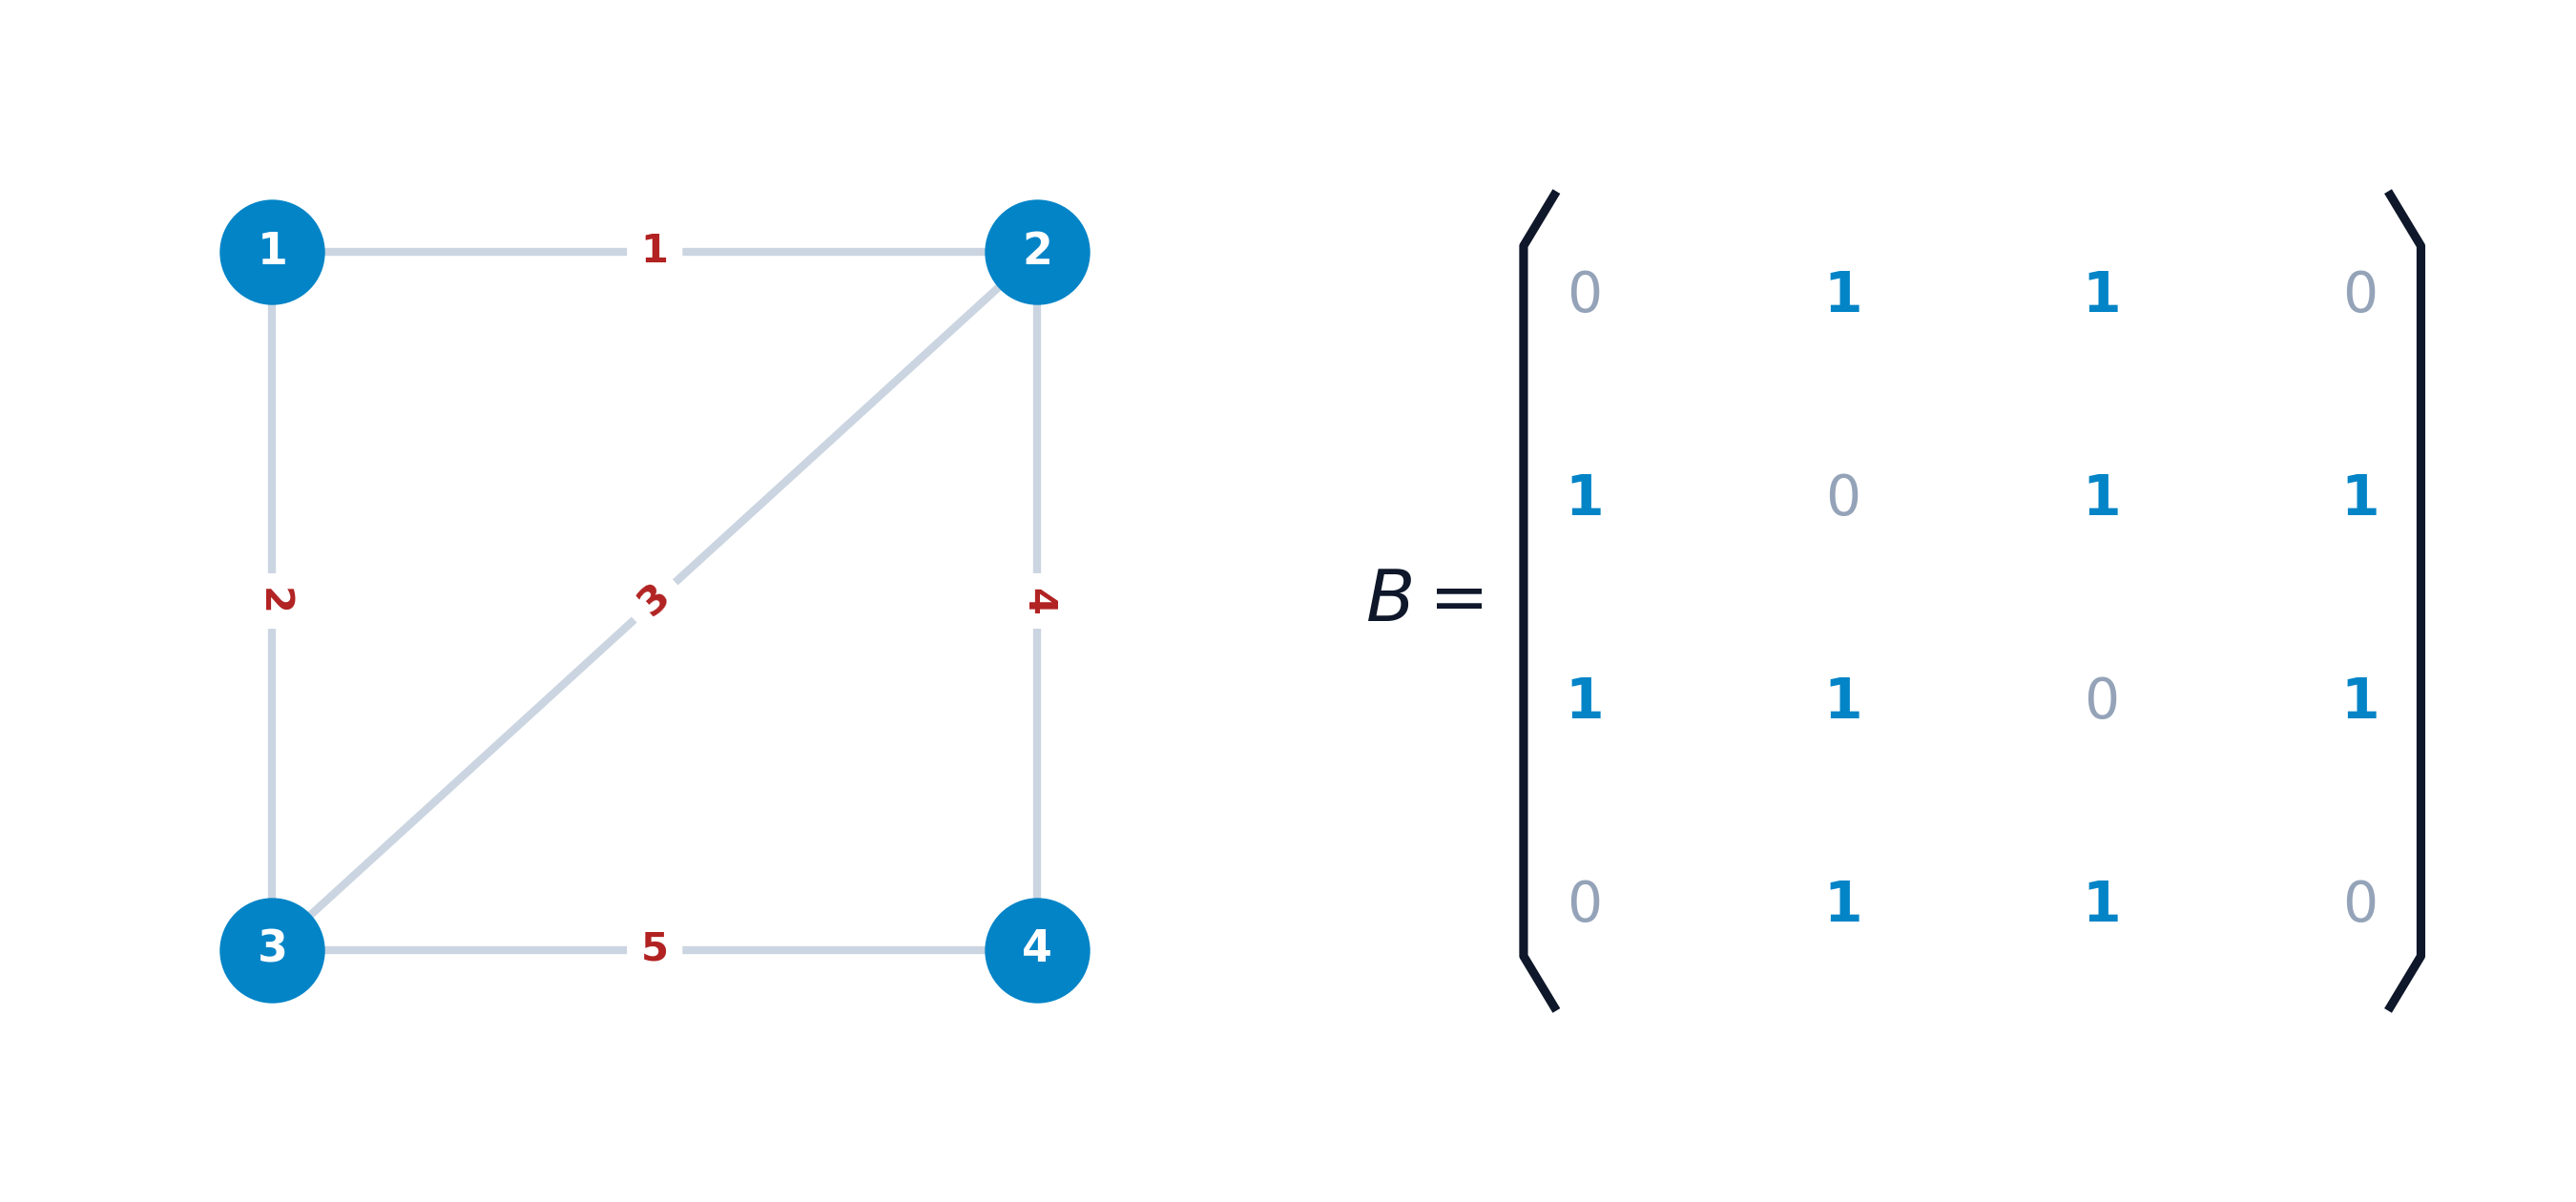
\includegraphics[width=0.8\linewidth,height=\textheight,keepaspectratio]{images/matriz_adyacencia_grafo.png}

}

\caption{\label{fig-matriz-adyacencia-grafo}Grafo no dirigido y su
correspondiente matriz de adyacencia simétrica B}

\end{figure}%

En el caso de redes dirigidas, la matriz de adyacencia registra la
dirección efectiva de los arcos entre vértices.

\begin{tcolorbox}[enhanced jigsaw, toprule=.15mm, opacitybacktitle=0.6, coltitle=black, colbacktitle=quarto-callout-note-color!10!white, title=\textcolor{quarto-callout-note-color}{\faInfo}\hspace{0.5em}{Definición: Matriz de adyacencia de un digrafo}, arc=.35mm, rightrule=.15mm, toptitle=1mm, breakable, bottomtitle=1mm, titlerule=0mm, colback=white, opacityback=0, leftrule=.75mm, colframe=quarto-callout-note-color-frame, left=2mm, bottomrule=.15mm]

Dado un digrafo \(G = (V, U)\) con \(n\) vértices y \(m\) arcos, la
\textbf{matriz de adyacencia} es una matriz cuadrada
\(B = (b_{ik}) \in \mathbb{R}^{n \times n}\) definida por: \[
b_{ik} = \begin{cases}
1 & \text{si } (i, k) \in U \text{ (existe un arco dirigido desde el nodo } i \text{ hacia el nodo } k\text{)}, \\
0 & \text{en otro caso.}
\end{cases}
\]

\end{tcolorbox}

Para un digrafo general, la matriz de adyacencia \(B\) es
\textbf{asimétrica} (\(B \neq B^T\)). La suma de los elementos de la
fila \(i\) indica el grado de salida del nodo
(\(d^+(i) = \sum_{k=1}^n b_{ik}\)), mientras que la suma de los
elementos de la columna \(k\) representa el grado de entrada
(\(d^-(k) = \sum_{i=1}^n b_{ik}\)). Como propiedad analítica adicional,
el elemento \((B^p)_{ik}\) de la \(p\)-ésima potencia de la matriz
\(B^p\) computa el número exacto de caminos orientados de longitud \(p\)
existentes entre el nodo \(i\) y el nodo \(k\). En la
Figura~\ref{fig-matriz-adyacencia-digrafo} se ilustra la matriz de
adyacencia asimétrica asociada a la red dirigida.

\begin{figure}

\centering{

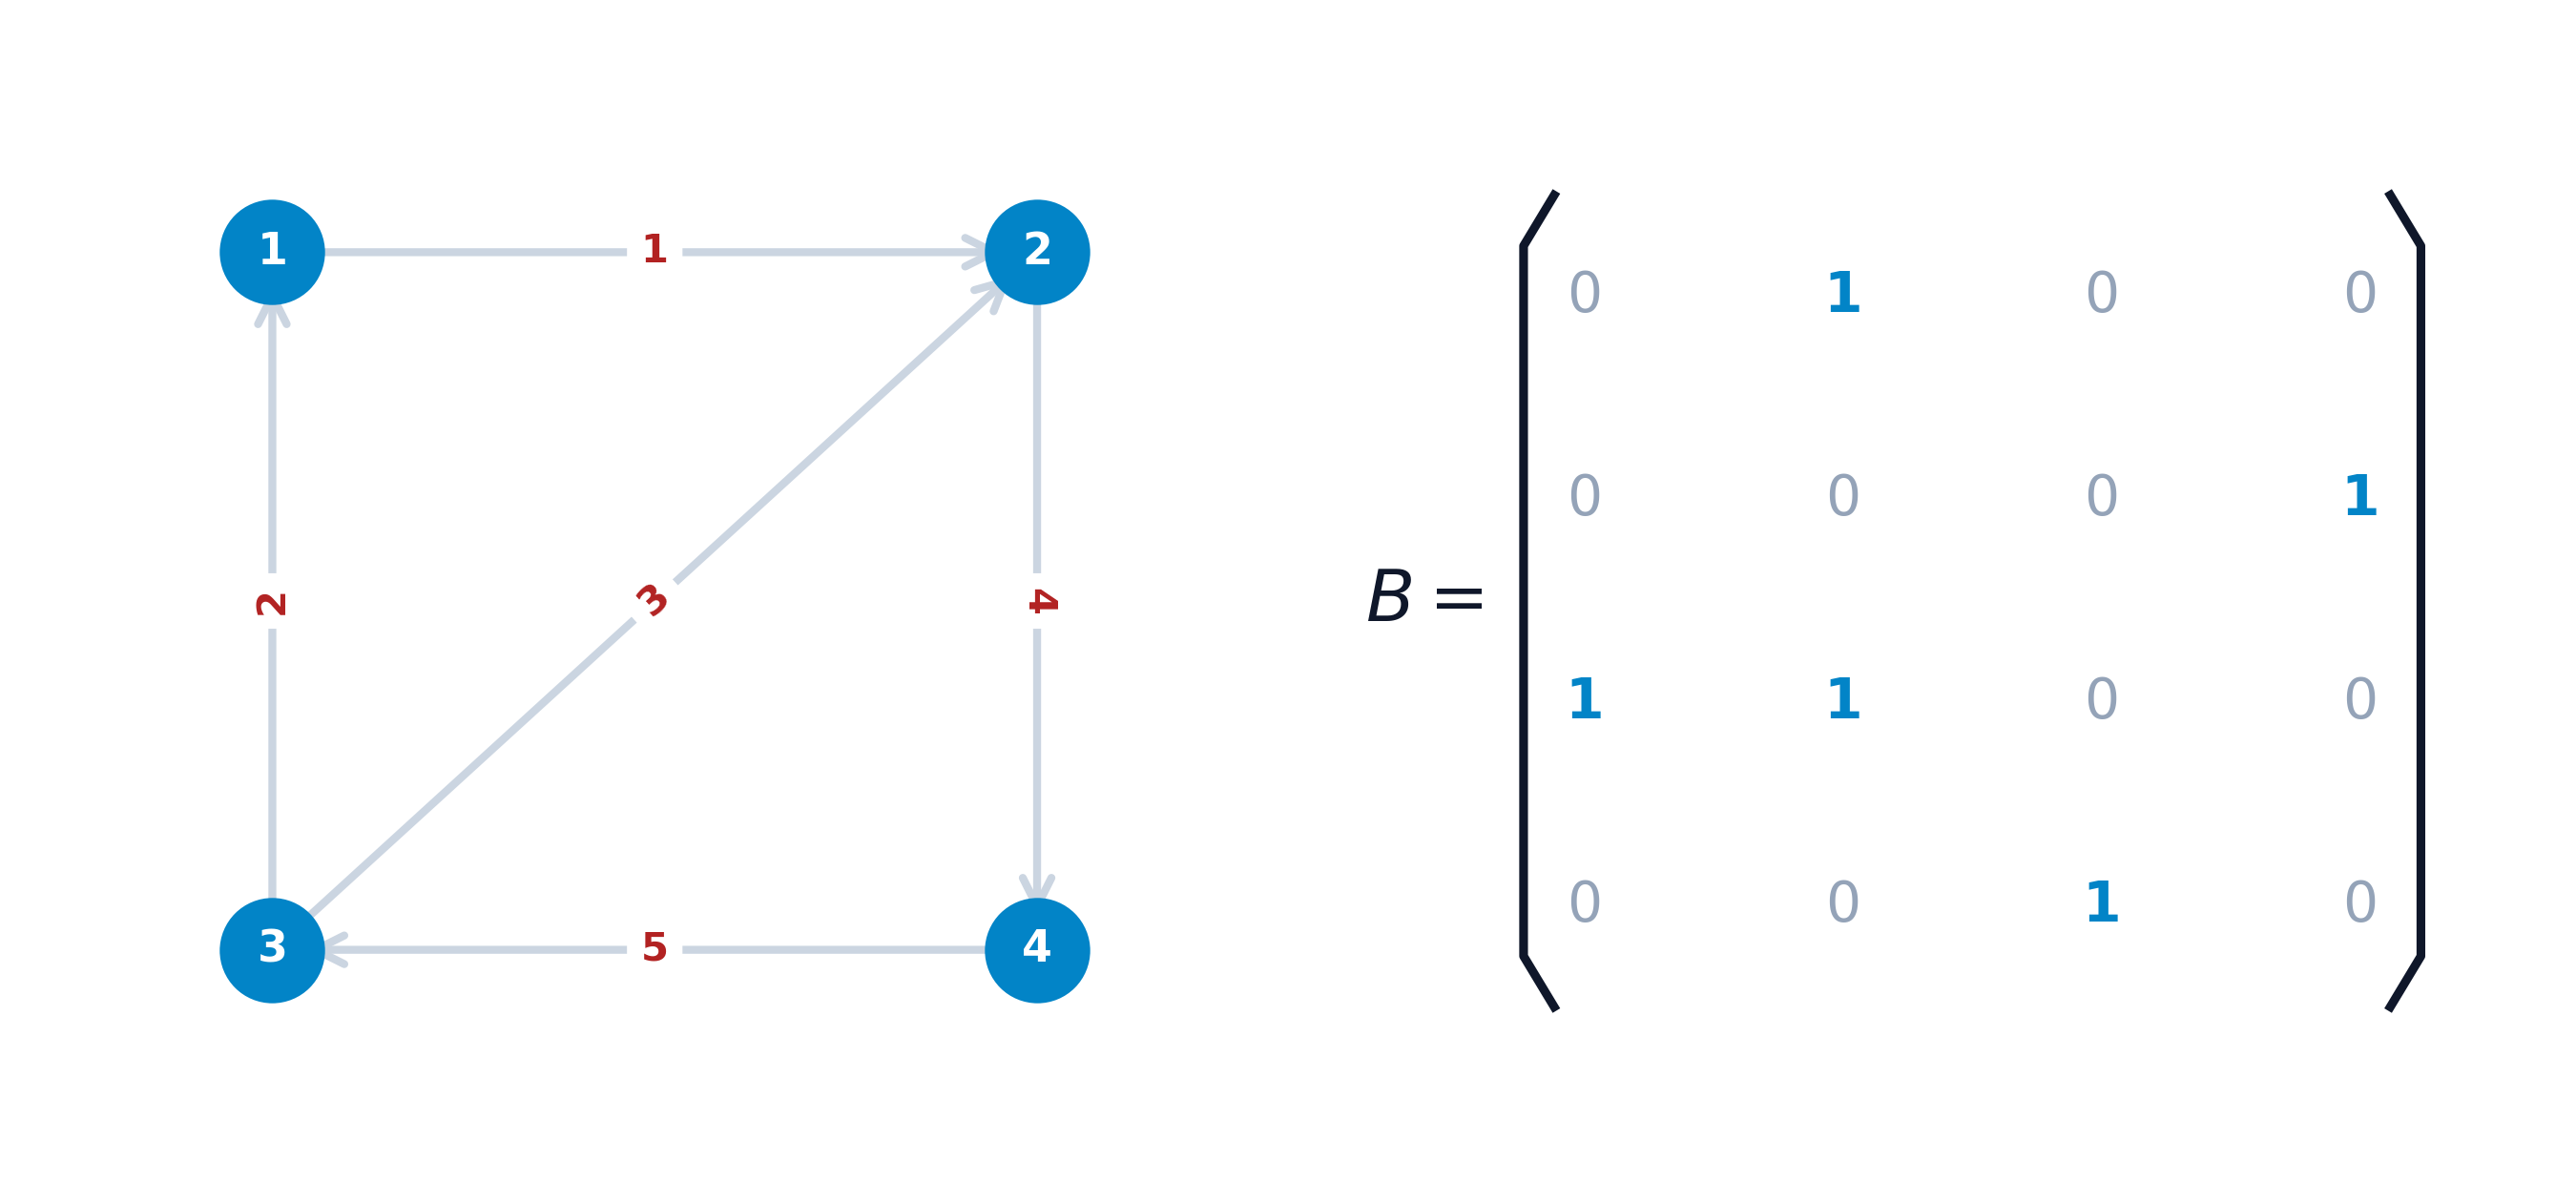
\includegraphics[width=0.8\linewidth,height=\textheight,keepaspectratio]{images/matriz_adyacencia_digrafo.png}

}

\caption{\label{fig-matriz-adyacencia-digrafo}Digrafo de muestra y su
correspondiente matriz de adyacencia asimétrica B}

\end{figure}%

A pesar de su claridad conceptual, la representación de redes mediante
matrices densas (de dimensiones \(n \times m\) para la incidencia o
\(n \times n\) para la adyacencia) presenta serias limitaciones de
eficiencia computacional cuando se trabaja con redes reales de gran
escala. Por ejemplo, en una red de infraestructuras o comunicaciones con
\(n = 10\,000\) vértices y \(m = 30\,000\) arcos, almacenar la matriz de
incidencia completa requeriría aproximadamente: \[
n \cdot m \cdot 1 \text{ byte} = 10\,000 \times 30\,000 \text{ bytes} = 3 \times 10^8 \text{ bytes} \approx 300\,000 \text{ KB} = 300 \text{ MB}
\] Sin embargo, dado que en la matriz de adyacencia solo \(30\,000\) de
las \(n^2 = 100\,000\,000\) entradas son distintas de cero (una densidad
de apenas el \(0.03\%\)), y en la matriz de incidencia solo
\(2m = 60\,000\) de los \(300\,000\,000\) elementos son no nulos
(densidad del \(0.02\%\)), la inmensa mayoría de la memoria almacenaría
ceros redundantes.

Por este motivo, los algoritmos de optimización de redes y los entornos
de computación científica emplean estructuras de datos dispersas
(\emph{sparse formats}) o \textbf{listas de adyacencia} para reducir el
coste de memoria linealmente a \(O(n + m)\).

\begin{center}\rule{0.5\linewidth}{0.5pt}\end{center}

\subsection{Representación vectorial}\label{representaciuxf3n-vectorial}

Para superar las limitaciones de memoria y la ineficiencia de las
matrices densas (de adyacencia o incidencia), la teoría computacional de
redes utiliza el esquema de \textbf{representación vectorial de dos
vectores}. Este método permite almacenar la topología completa de un
digrafo o grafo utilizando únicamente dos vectores unidimensionales: un
vector \(\alpha\) de punteros o índices de dimensión \(n + 1\), y un
vector \(\beta\) de nodos de destino de dimensión \(m\) (o de las
aristas consideradas para grafos no dirigidos).

El máximo ahorro de memoria se consigue ordenando previamente el
conjunto de arcos o aristas en \textbf{orden lexicográfico}.

\begin{tcolorbox}[enhanced jigsaw, toprule=.15mm, opacitybacktitle=0.6, coltitle=black, colbacktitle=quarto-callout-note-color!10!white, title=\textcolor{quarto-callout-note-color}{\faInfo}\hspace{0.5em}{Definición: Orden lexicográfico de arcos}, arc=.35mm, rightrule=.15mm, toptitle=1mm, breakable, bottomtitle=1mm, titlerule=0mm, colback=white, opacityback=0, leftrule=.75mm, colframe=quarto-callout-note-color-frame, left=2mm, bottomrule=.15mm]

\begin{enumerate}
\def\labelenumi{\arabic{enumi}.}
\item
  \(i_1 \le i_2 \le \dots \le i_m\) (los arcos se agrupan ordenados por
  su nodo de origen).
\item
  Si \(i_k = i_{k+1}\), entonces \(j_k \le j_{k+1}\) (en caso de empate
  en el origen, se ordenan por su nodo de destino).
\end{enumerate}

\end{tcolorbox}

Una vez establecidos los arcos en orden lexicográfico, se construyen los
dos vectores estructurales \(\beta\) y \(\alpha\):

\begin{tcolorbox}[enhanced jigsaw, toprule=.15mm, opacitybacktitle=0.6, coltitle=black, colbacktitle=quarto-callout-note-color!10!white, title=\textcolor{quarto-callout-note-color}{\faInfo}\hspace{0.5em}{Definición: Construcción de los vectores estructurales \(\beta\) y
\(\alpha\)}, arc=.35mm, rightrule=.15mm, toptitle=1mm, breakable, bottomtitle=1mm, titlerule=0mm, colback=white, opacityback=0, leftrule=.75mm, colframe=quarto-callout-note-color-frame, left=2mm, bottomrule=.15mm]

\begin{enumerate}
\def\labelenumi{\arabic{enumi}.}
\item
  \textbf{Vector de destinos \(\beta\)} (de dimensión \(m\)): Almacena
  secuencialmente en la posición \(k\)-ésima el vértice de llegada o
  destino del \(k\)-ésimo arco ordenado: \[
  \beta(k) = j_k, \quad \forall k \in \{1, \dots, m\}.
  \]
\item
  \textbf{Vector de punteros de inicio \(\alpha\)} (de dimensión
  \(n + 1\)): Determina la posición de memoria en \(\beta\) donde
  comienza la lista de arcos que parten de cada nodo \(i \in V\). Se
  define mediante el valor frontera \(\alpha(n + 1) = m + 1\) y la
  relación de recurrencia regresiva (para \(k = n, n-1, \dots, 1\)): \[
  \alpha(k) = \alpha(k + 1) - d^+(k),
  \] donde \(d^+(k)\) denota el grado de salida (número de arcos
  salientes) del nodo \(k\).
\end{enumerate}

\end{tcolorbox}

\begin{figure}

\centering{

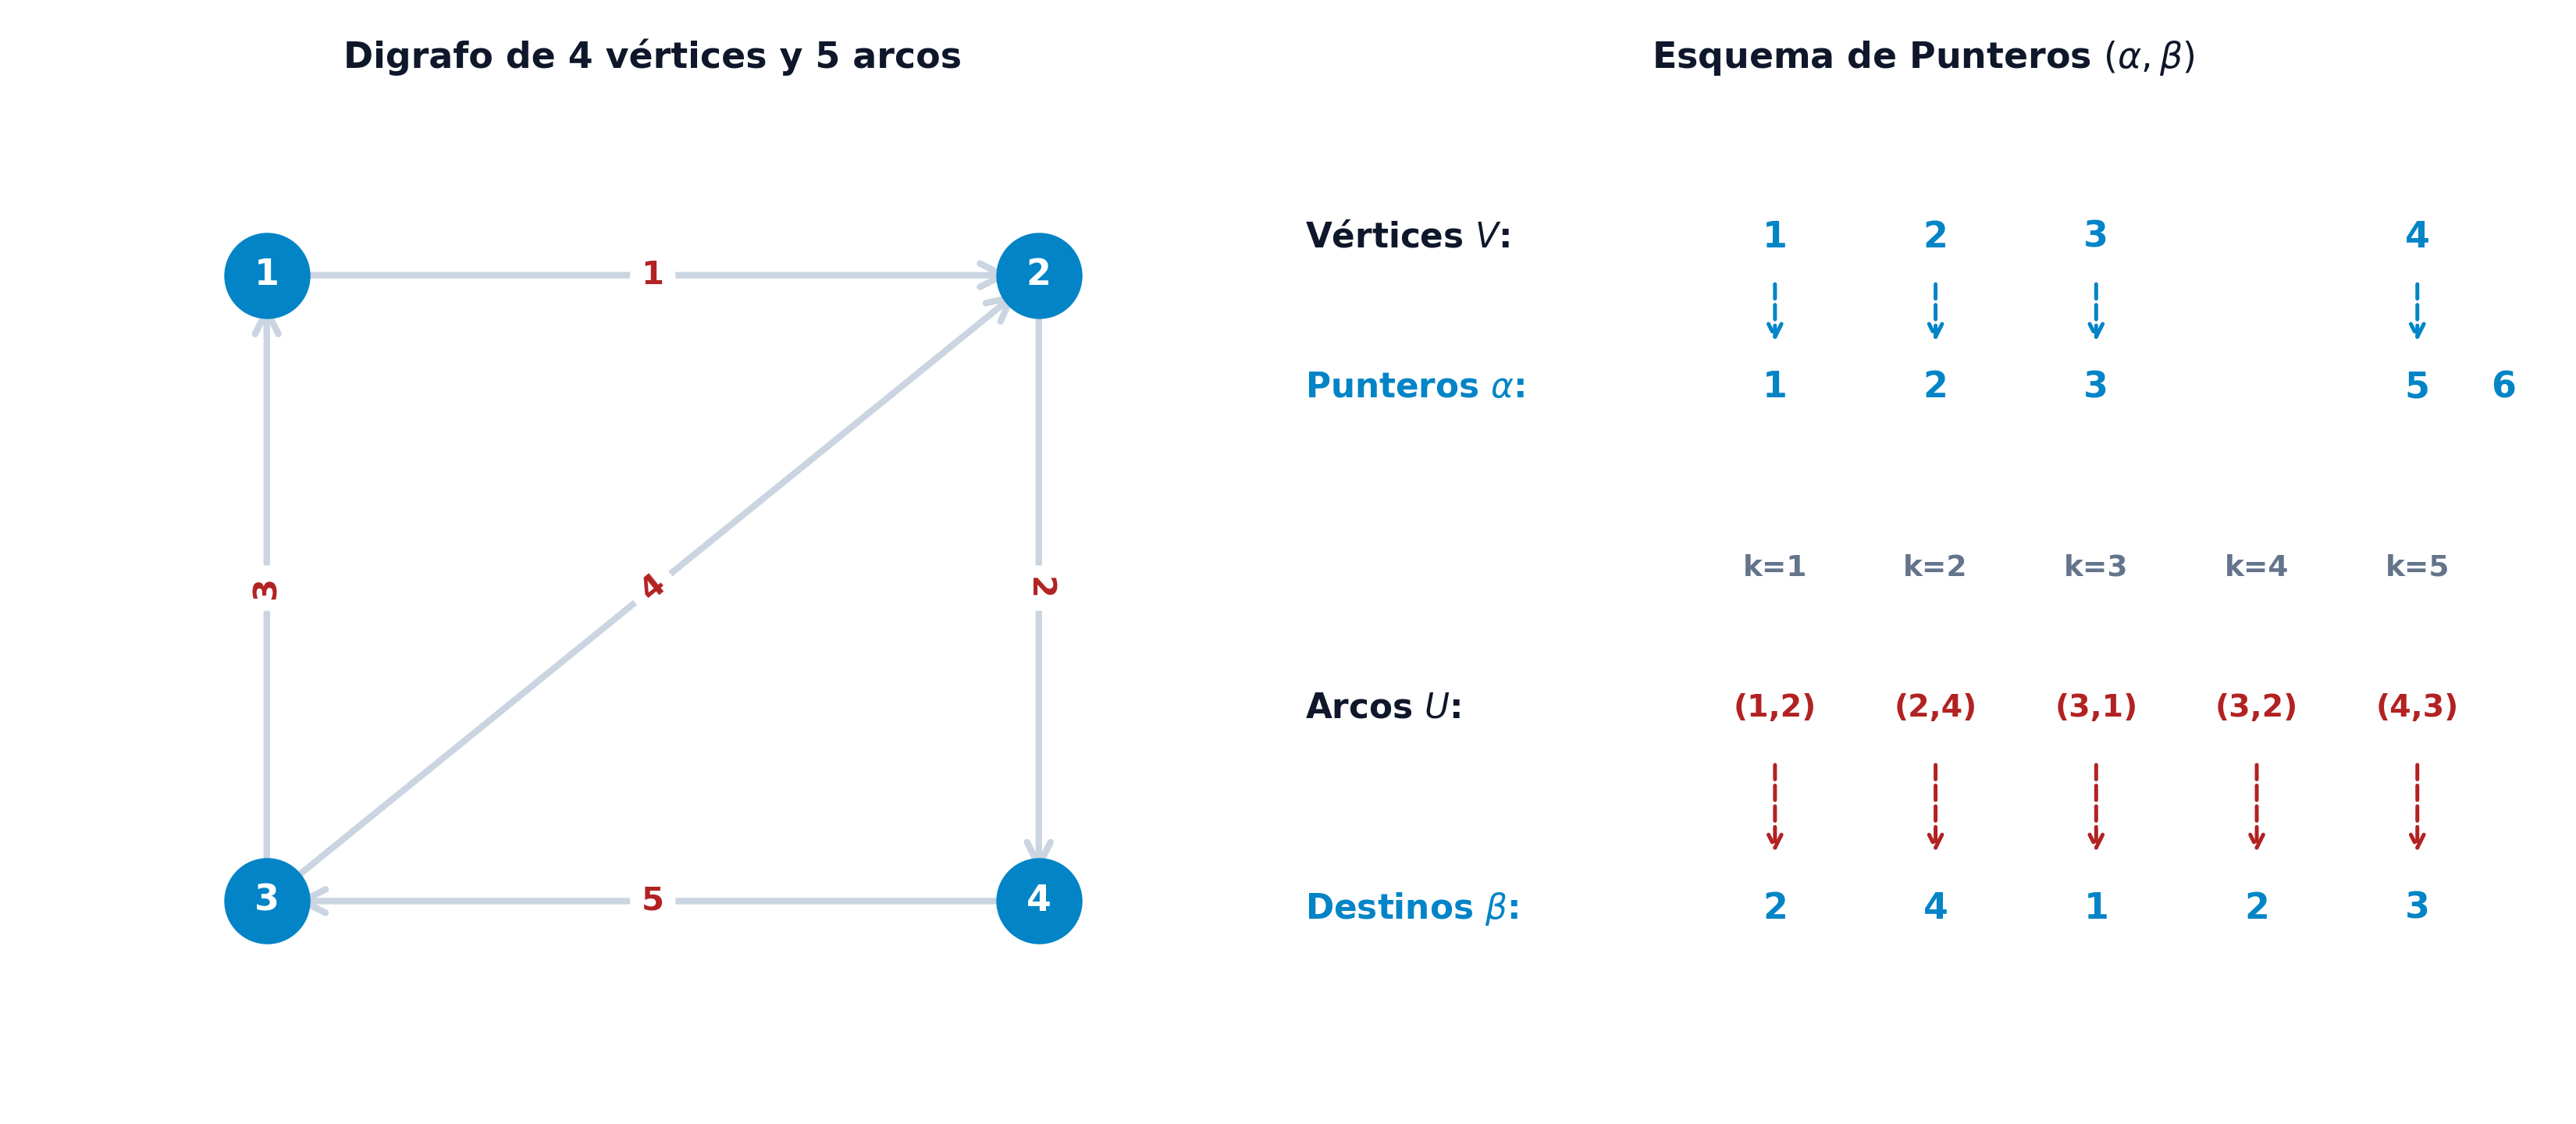
\includegraphics[width=0.85\linewidth,height=\textheight,keepaspectratio]{images/representacion_vectorial_digrafo.png}

}

\caption{\label{fig-representacion-vectorial-digrafo}Digrafo de 4
vértices y la construcción explícita de sus vectores alfa y beta}

\end{figure}%

Como se aprecia detalladamente en la
Figura~\ref{fig-representacion-vectorial-digrafo}, la correspondencia
entre la topología del digrafo y la memoria se articula a través de tres
niveles de lectura:

\begin{itemize}
\tightlist
\item
  \textbf{Ordenación lexicográfica del conjunto de arcos \(U\)}: Los 5
  arcos se ordenan según su nodo de origen y destino, generando la
  secuencia indexada \(k=1, \dots, 5\): el arco \(k=1\) es \((1,2)\), el
  arco \(k=2\) es \((2,4)\), los arcos \(k=3\) y \(k=4\) son \((3,1)\) y
  \((3,2)\), y el arco \(k=5\) es \((4,3)\).
\item
  \textbf{Construcción directa de \(\beta\)}: El vector
  \(\beta = (2, 4, 1, 2, 3)\) registra únicamente los nodos de llegada
  de cada uno de los arcos ordenados en la fila \(U\).
\item
  \textbf{Construcción regresiva de \(\alpha\)}: Se parte de la
  condición frontera \(\alpha(5) = m + 1 = 6\). A continuación, se
  descuenta el grado de salida de cada nodo de derecha a izquierda:

  \begin{itemize}
  \tightlist
  \item
    Para el nodo 4 (\(d^+(4) = 1\) arco saliente, \((4,3)\)), la
    posición inicial es \(\alpha(4) = 6 - 1 = 5\).
  \item
    Para el nodo 3 (\(d^+(3) = 2\) arcos salientes, \((3,1)\) y
    \((3,2)\)), la posición inicial es \(\alpha(3) = 5 - 2 = 3\).
  \item
    Para el nodo 2 (\(d^+(2) = 1\) arco saliente, \((2,4)\)), la
    posición inicial es \(\alpha(2) = 3 - 1 = 2\).
  \item
    Para el nodo 1 (\(d^+(1) = 1\) arco saliente, \((1,2)\)), la
    posición inicial es \(\alpha(1) = 2 - 1 = 1\).
  \end{itemize}
\end{itemize}

De este modo, para recuperar los sucesores de cualquier nodo \(i\) basta
consultar la sublista de \(\beta\) entre las posiciones \(\alpha(i)\) y
\(\alpha(i+1) - 1\). Por ejemplo, para el nodo 3, se examinan los
índices desde \(\alpha(3) = 3\) hasta \(\alpha(4) - 1 = 4\), obteniendo
inmediatamente los nodos de destino \(\beta(3) = 1\) y \(\beta(4) = 2\),
correspondientes a los arcos \((3,1)\) y \((3,2)\).

\begin{figure}

\centering{

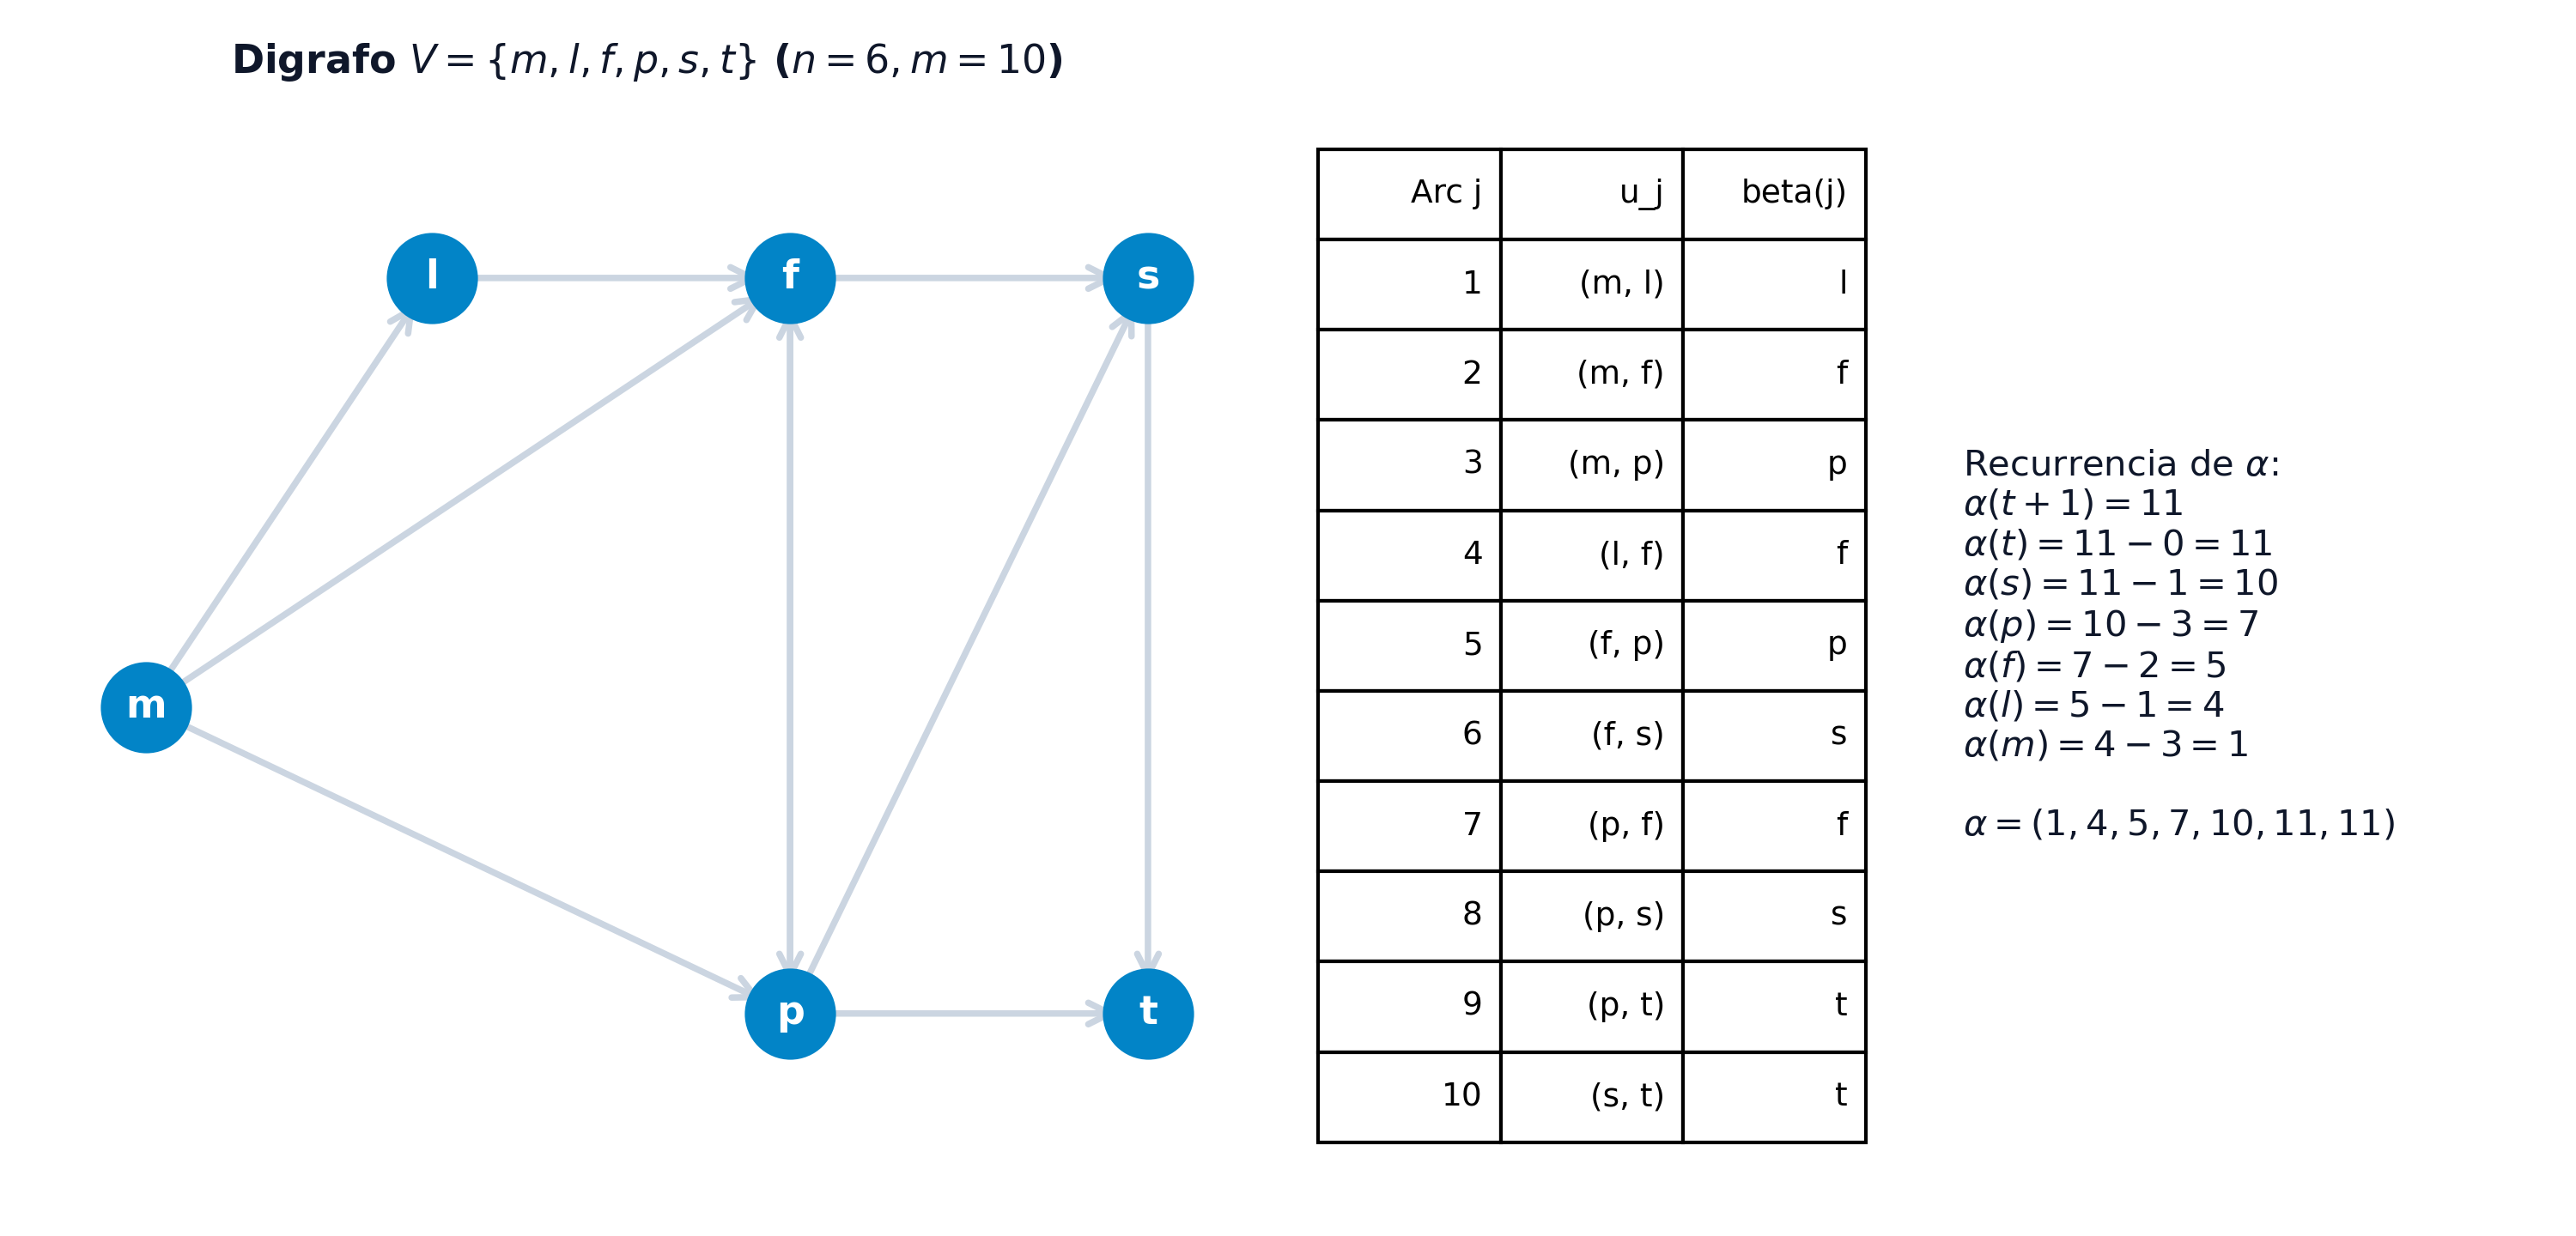
\includegraphics[width=0.9\linewidth,height=\textheight,keepaspectratio]{images/representacion_vectorial_ejemplo_complejo.png}

}

\caption{\label{fig-representacion-vectorial-ejemplo-complejo}Digrafo de
6 vértices, tabla de arcos ordenados y deducción regresiva del vector
alfa}

\end{figure}%

El esquema de representación mediante dos vectores se extiende de forma
totalmente natural a los \textbf{grafos no dirigidos}. Para ello, cada
arista no dirigida \(\{u, v\}\) se considera equivalente a un par de
conexiones salientes considerando ambas orientaciones posibles. Así, una
arista no dirigida contribuirá con una entrada en el vector \(\beta\)
por cada nodo extremo donde es incidente, y el vector \(\alpha\) se
construye utilizando la cantidad de aristas que parten de cada nodo
según el orden lexicográfico prefijado de las parejas. En la
Figura~\ref{fig-representacion-vectorial-grafo-nodirigido} se muestra la
extensión vectorial aplicada a un grafo no dirigido sobre 5 vértices y 7
aristas.

\begin{figure}

\centering{

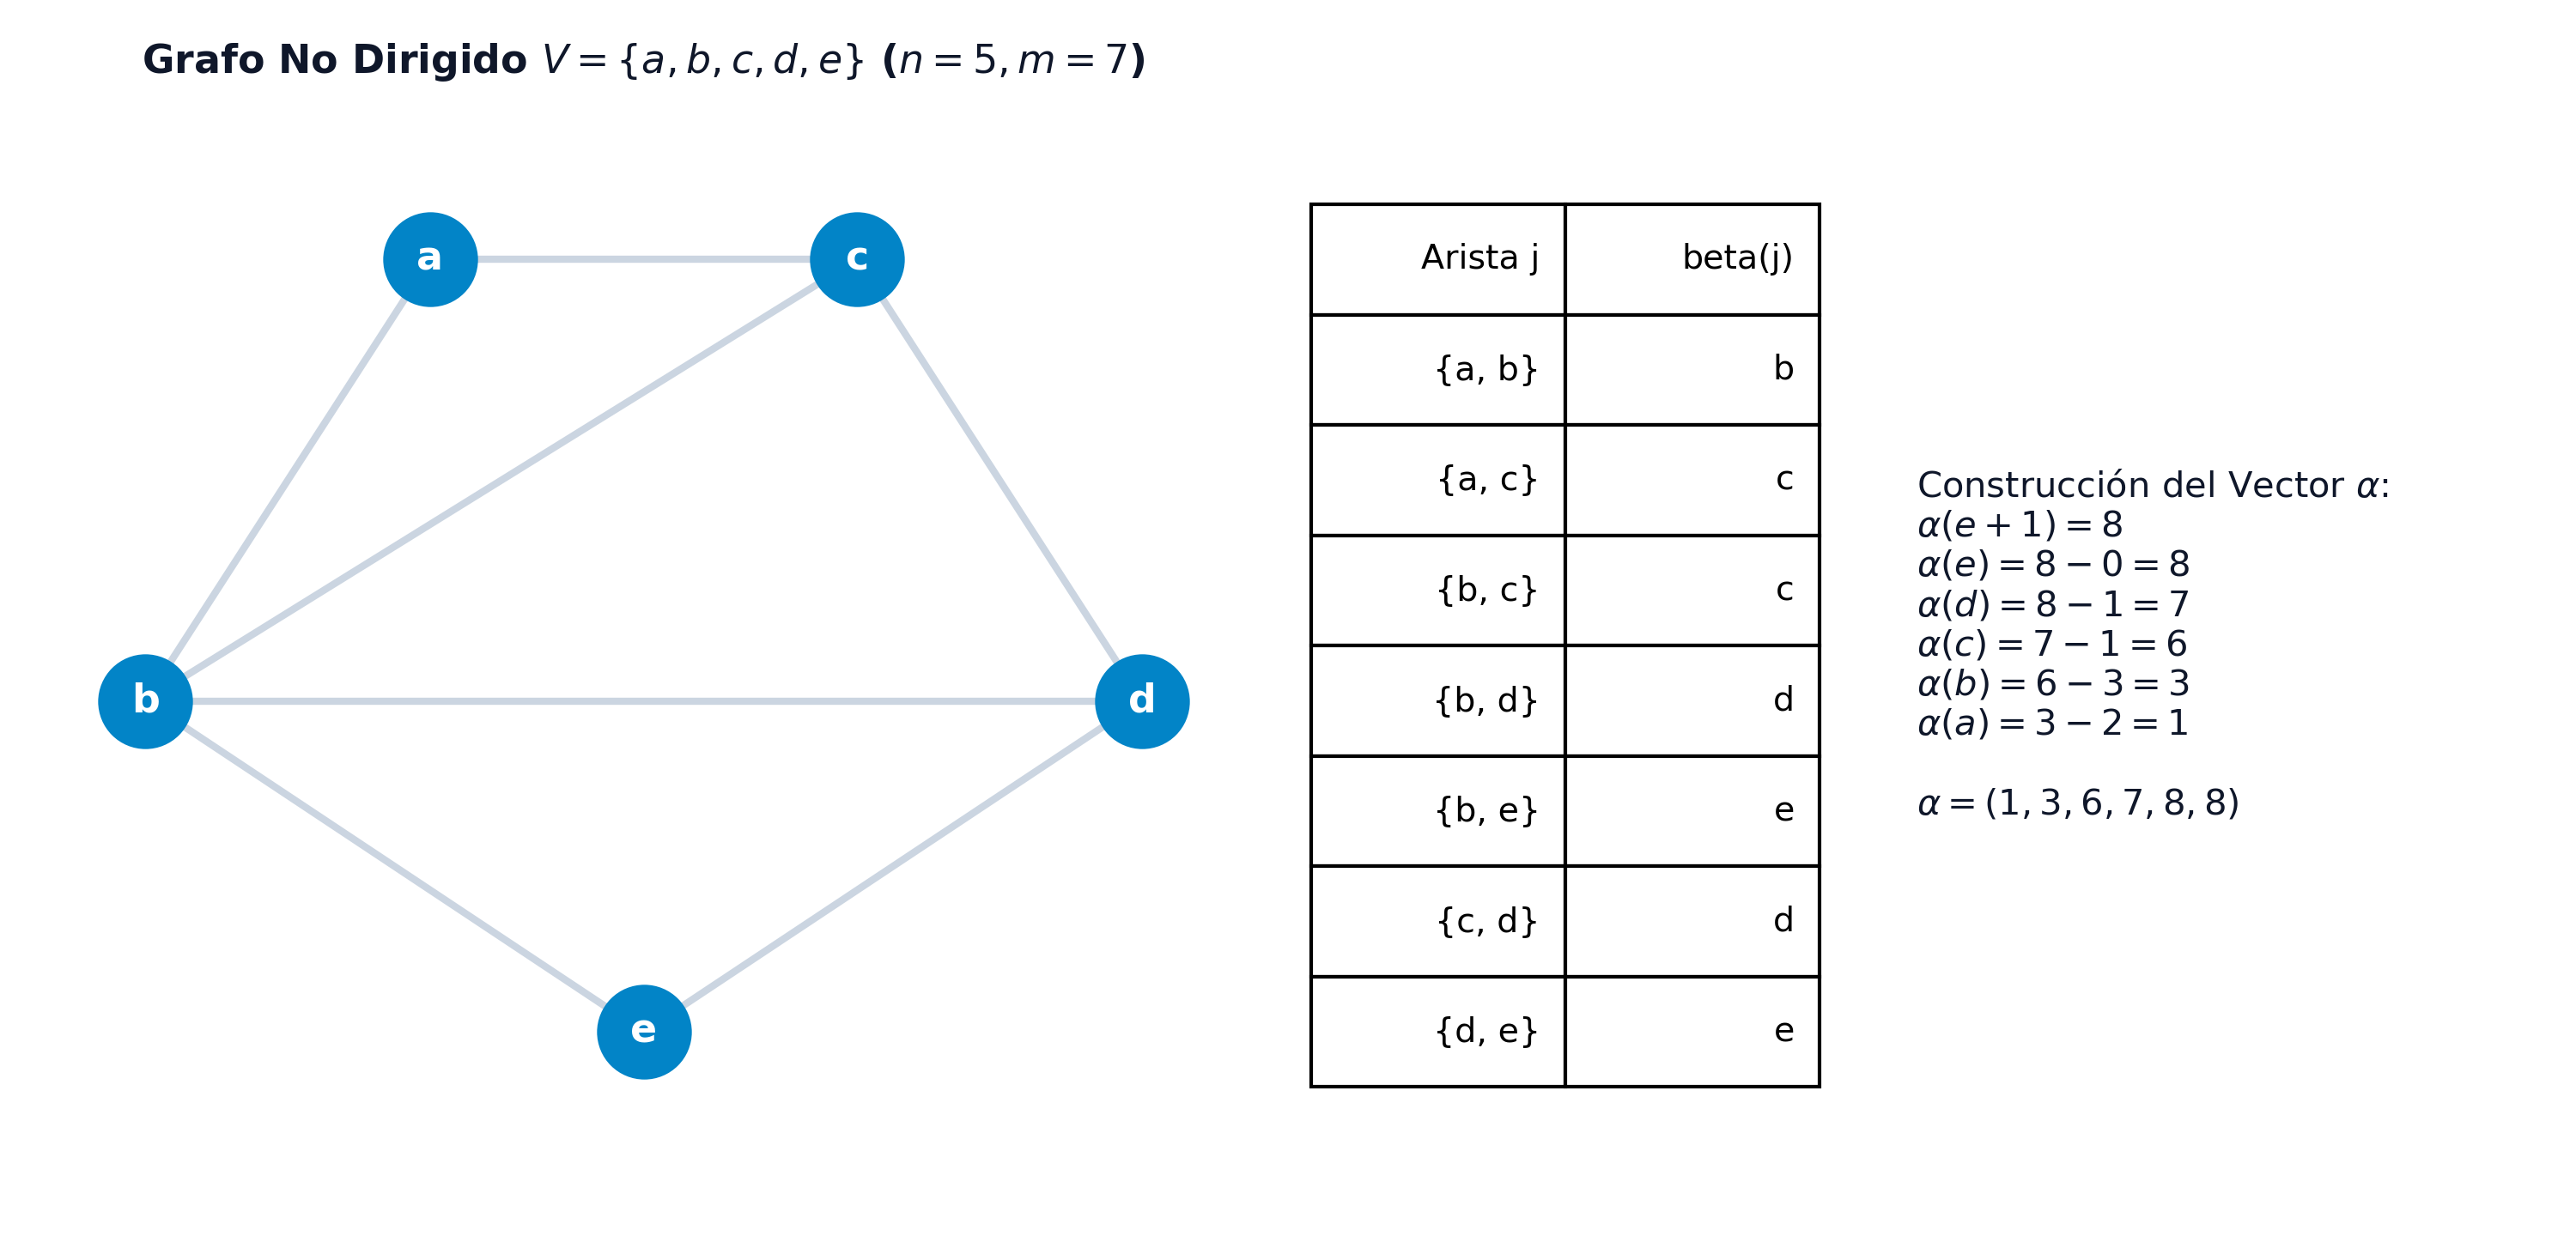
\includegraphics[width=0.9\linewidth,height=\textheight,keepaspectratio]{images/representacion_vectorial_grafo_nodirigido.png}

}

\caption{\label{fig-representacion-vectorial-grafo-nodirigido}Grafo no
dirigido sobre 5 vértices y su representación vectorial mediante
vectores alfa y beta}

\end{figure}%

\begin{center}\rule{0.5\linewidth}{0.5pt}\end{center}

\subsection{Representación por listas de
adyacencia}\label{representaciuxf3n-por-listas-de-adyacencia}

Frente al almacenamiento estático prefijado que exigen las matrices
densas (de adyacencia o incidencia) o las estructuras vectoriales
compactas como el vector \(\alpha\), la \textbf{representación por
listas de adyacencia} constituye la alternativa computacional más
flexible para gestionar redes dinámicas. Este método consiste en asociar
a cada vértice \(v \in V\) del grafo o digrafo una lista dinámicamente
enlazada que contiene la secuencia de todos sus vértices sucesores (o
nodos adyacentes a los que apunta directamente).

\begin{tcolorbox}[enhanced jigsaw, toprule=.15mm, opacitybacktitle=0.6, coltitle=black, colbacktitle=quarto-callout-note-color!10!white, title=\textcolor{quarto-callout-note-color}{\faInfo}\hspace{0.5em}{Definición: Representación por listas de adyacencia}, arc=.35mm, rightrule=.15mm, toptitle=1mm, breakable, bottomtitle=1mm, titlerule=0mm, colback=white, opacityback=0, leftrule=.75mm, colframe=quarto-callout-note-color-frame, left=2mm, bottomrule=.15mm]

Dada una red \(G = (V, E)\) o \(G = (V, U)\) con \(n = |V|\) vértices,
la \textbf{representación por listas de adyacencia} asigna a cada nodo
\(i \in V\) una lista de punteros dinámicos \(\text{Adj}[i]\) formada
por la colección ordenada de vértices adyacentes a los que se conecta:
\[
\text{Adj}[i] = \{ j \in V \mid (i, j) \in U \text{ o } \{i, j\} \in E \}.
\]

\end{tcolorbox}

La ventaja fundamental de este esquema reside en que las listas de
adyacencia no requieren dimensionarse ni reservarse de forma estática
antes de comenzar los cálculos, haciendo un uso eficiente de la
asignación dinámica de memoria mediante punteros o nodos enlazados. Esta
flexibilidad estructural permite modificar la red en tiempo real
(añadiendo o eliminando vértices y conexiones sin necesidad de
reestructurar o copiar bloques contiguos de memoria), lo que convierte a
esta representación en la opción óptima para modelar grafos en evolución
temporal o algoritmos de exploración probabilística.

En la Figura~\ref{fig-lista-adyacencia-digrafo} se ilustra la
arquitectura de datos dinámica para un digrafo dirigido compuesto por 6
vértices \(V = \{m, l, f, p, s, t\}\). La figura contrapone la topología
de la red a la izquierda con el vector cabecera de nodos y sus
correspondientes cadenas horizontales de punteros hacia los nodos de
destino.

\begin{figure}

\centering{

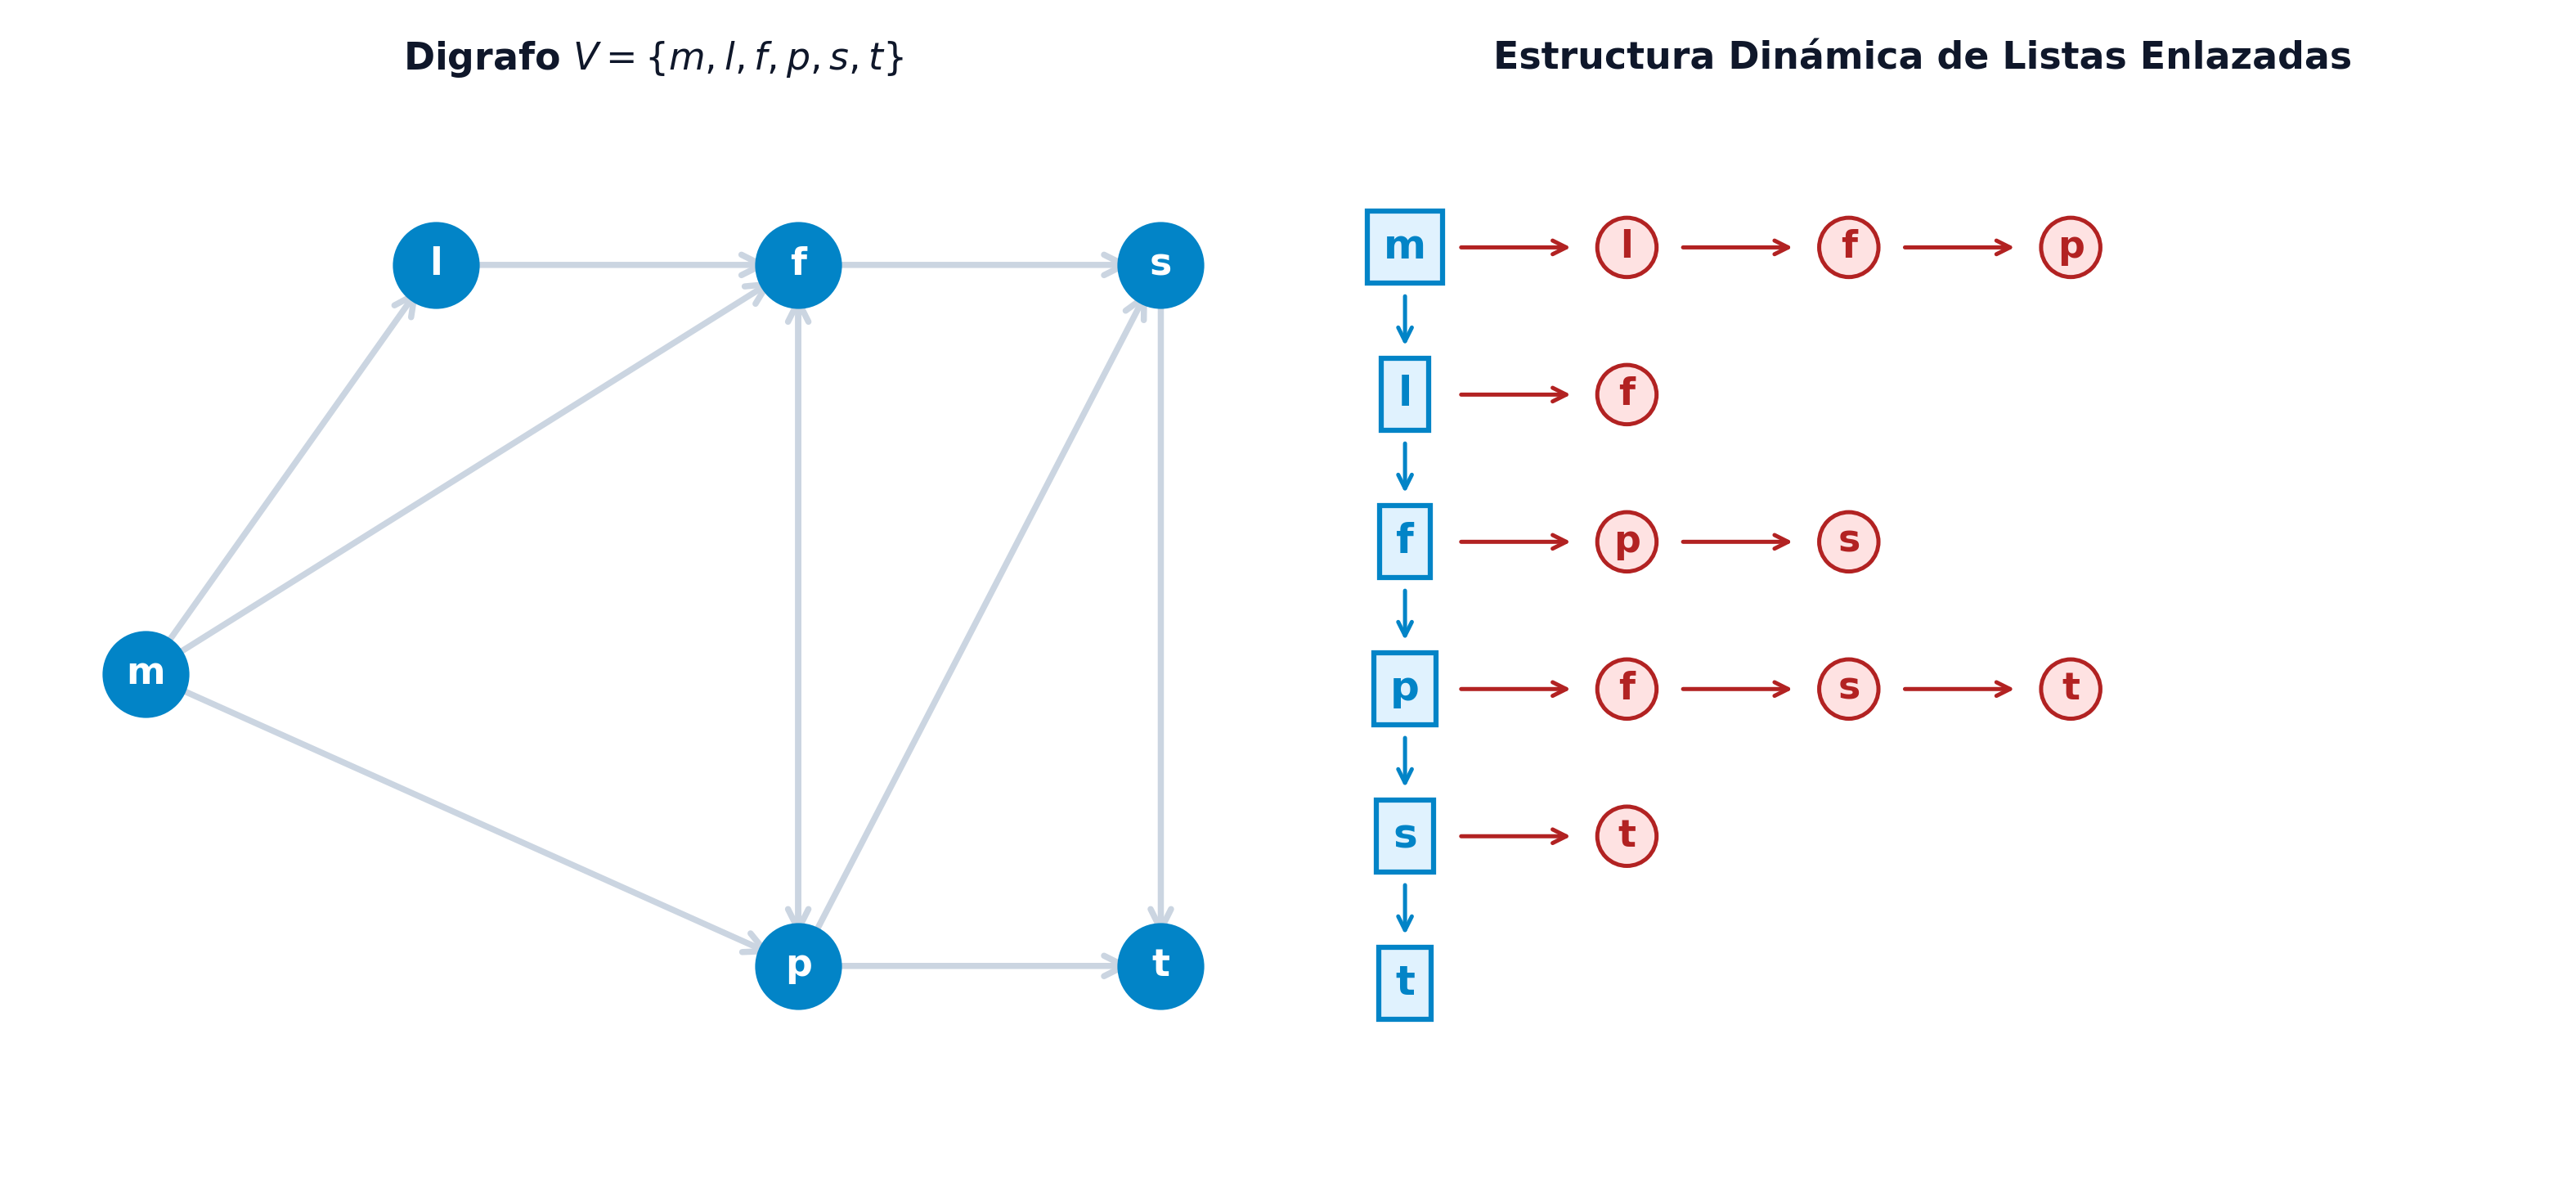
\includegraphics[width=0.9\linewidth,height=\textheight,keepaspectratio]{images/lista_adyacencia_digrafo.png}

}

\caption{\label{fig-lista-adyacencia-digrafo}Digrafo de 6 vértices y su
representación por listas de adyacencia dinámicamente enlazadas}

\end{figure}%

Como se observa en la Figura~\ref{fig-lista-adyacencia-digrafo}, la
cabecera vertical agrupa a los 6 vértices del digrafo, y cada fila
despliega horizontalmente la secuencia de sucesores enlazados:

\begin{itemize}
\tightlist
\item
  El nodo \(m\) encadena los vértices adyacentes salientes
  \(l \to f \to p\).
\item
  El nodo \(l\) encadena únicamente su único sucesor \(f\).
\item
  El nodo \(f\) encadena los vértices \(p \to s\).
\item
  El nodo \(p\) encadena tres destinos \(f \to s \to t\).
\item
  El nodo \(s\) se conecta con \(t\).
\item
  El nodo hundimiento \(t\) mantiene una lista vacía (\(\emptyset\)),
  reflejando que su grado de salida es \(d^+(t) = 0\).
\end{itemize}

El esquema de listas de adyacencia se extiende de manera inmediata a los
\textbf{grafos no dirigidos}. En este escenario, cada arista no dirigida
\(\{u, v\}\) genera dos entradas recíprocas en las estructuras
enlazadas: el nodo \(v\) se añade a la lista de adyacencia
\(\text{Adj}[u]\), y simétricamente el nodo \(u\) se incorpora a la
lista de adyacencia \(\text{Adj}[v]\). En la
Figura~\ref{fig-lista-adyacencia-grafo} se presenta la estructura de
listas enlazadas recíprocas para un grafo no dirigido sobre 5 vértices
\(V = \{a, b, c, d, e\}\).

\begin{figure}

\centering{

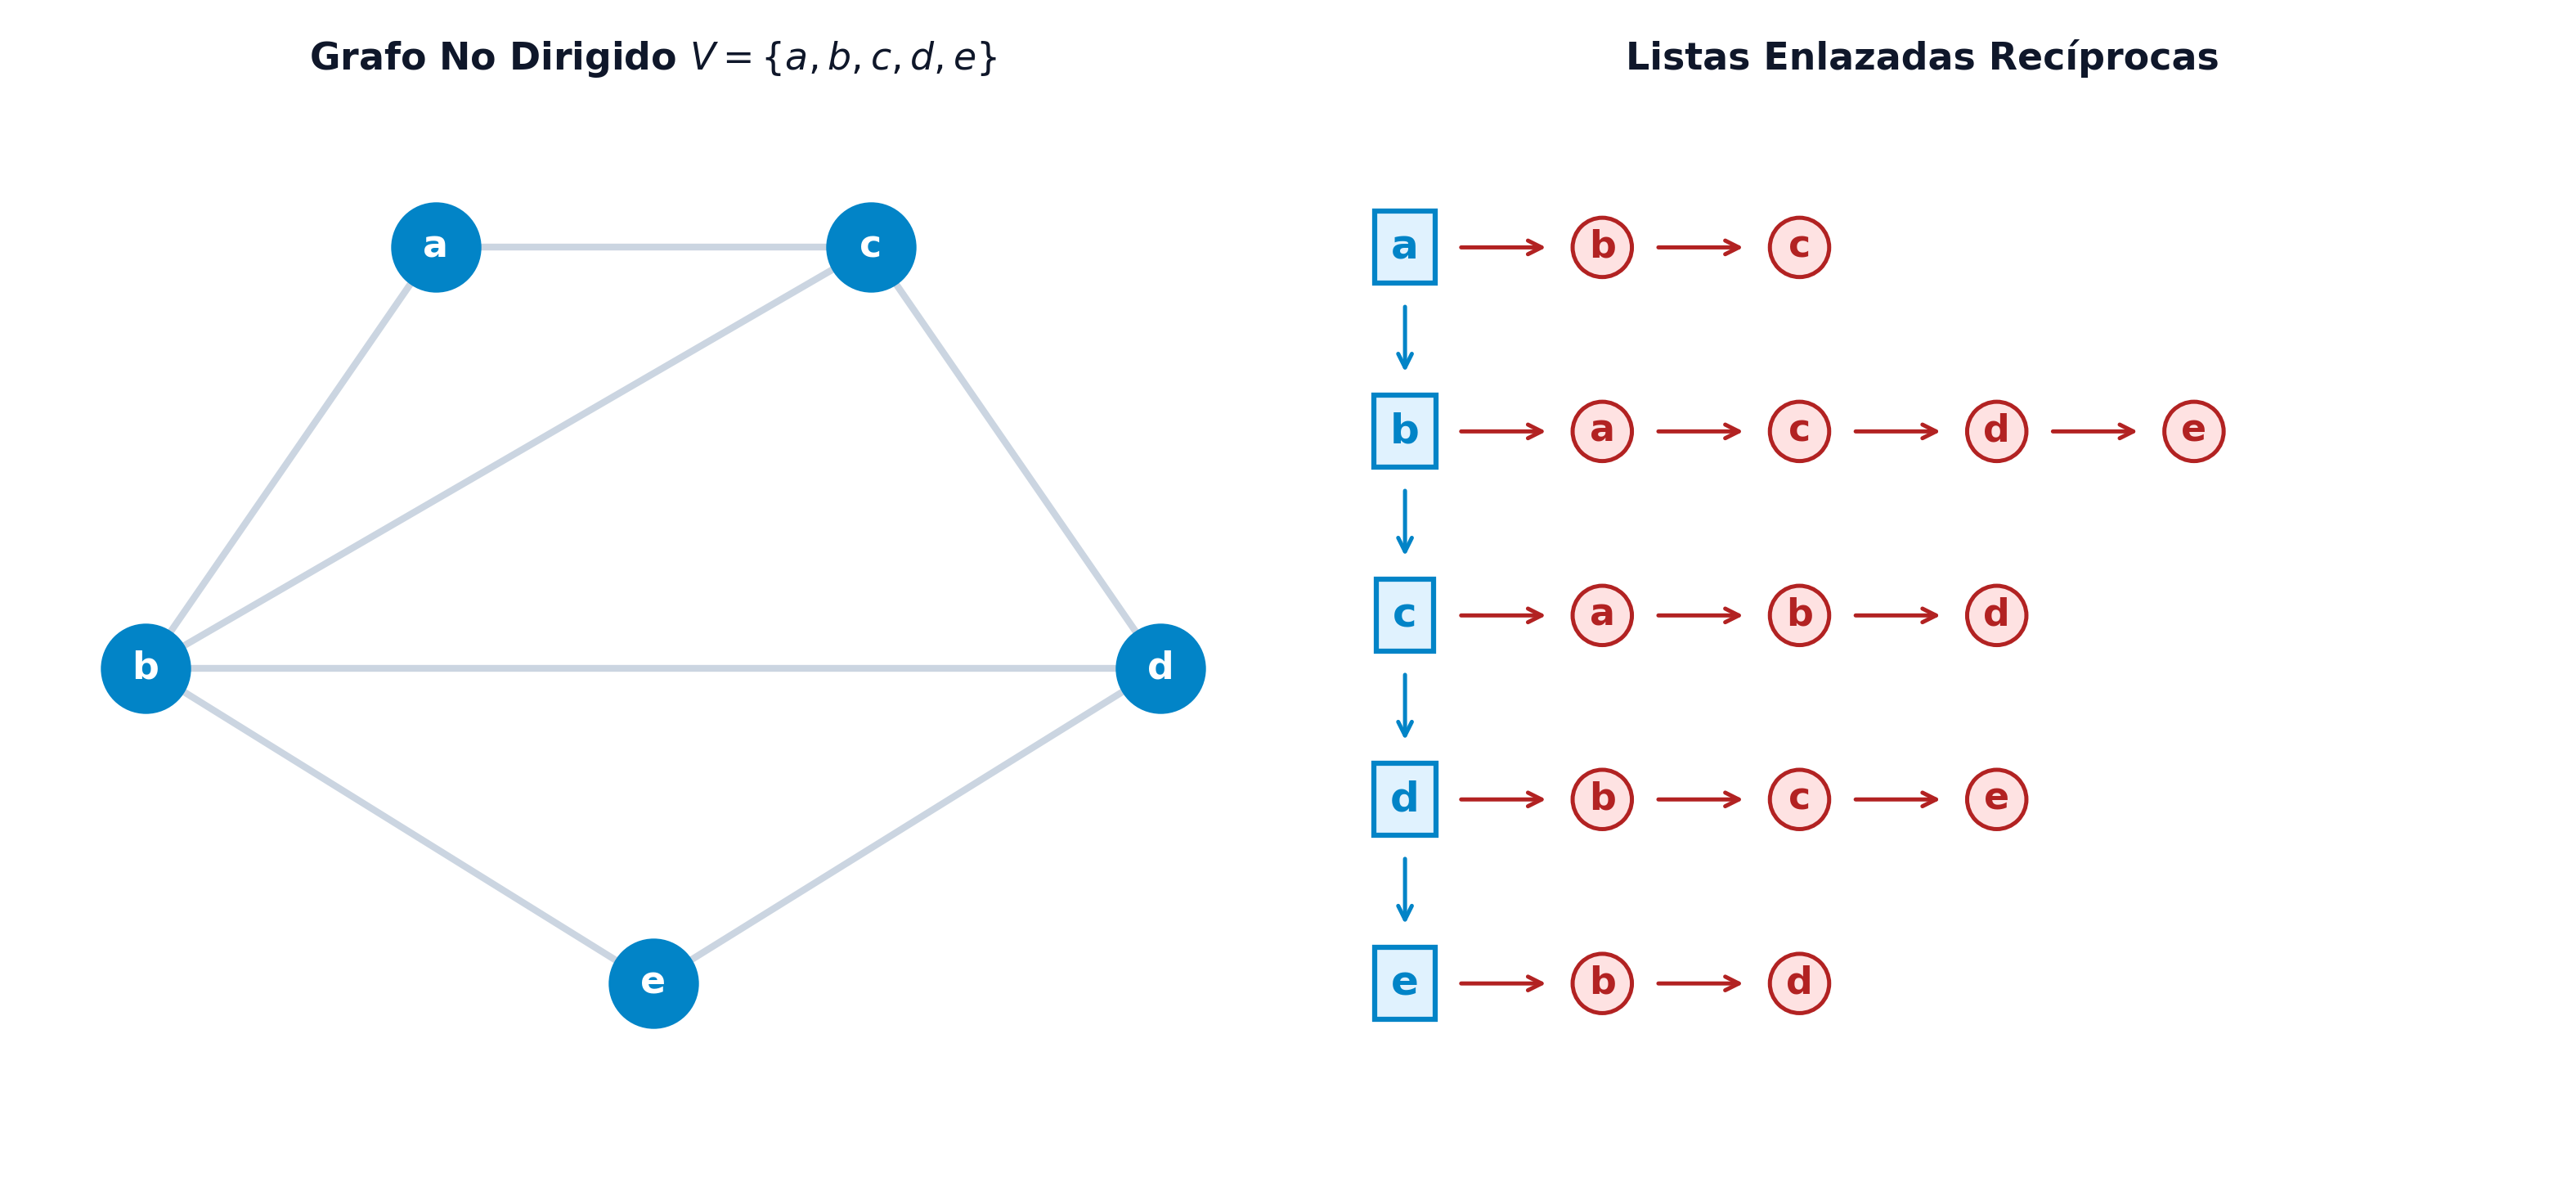
\includegraphics[width=0.9\linewidth,height=\textheight,keepaspectratio]{images/lista_adyacencia_grafo.png}

}

\caption{\label{fig-lista-adyacencia-grafo}Grafo no dirigido sobre 5
vértices y su representación por listas de adyacencia recíprocas}

\end{figure}%

Como ilustra la Figura~\ref{fig-lista-adyacencia-grafo}, la simetría de
las aristas no dirigidas se refleja en la presencia cruzada de los
vértices adyacentes: la arista \(\{a, b\}\) provoca que \(b\) figure en
\(\text{Adj}[a]\) (\(a \to b \to c\)) y que \(a\) figure en
\(\text{Adj}[b]\) (\(b \to a \to c \to d \to e\)). La suma total de los
elementos almacenados entre todas las listas enlazadas es exactamente
\(2m\), lo que garantiza un consumo espacial óptimo \(O(n + m)\) con
total versatilidad para la inserción y borrado dinámico de aristas.

\begin{center}\rule{0.5\linewidth}{0.5pt}\end{center}

\section{Estructura matemática de los
árboles}\label{estructura-matemuxe1tica-de-los-uxe1rboles}

Los árboles constituyen la clase más elemental y transversal de grafos
en la optimización combinatoria y el análisis de redes. Formalmente, un
árbol combina la propiedad de conexión global con la ausencia de
redundancia cíclica.

\begin{tcolorbox}[enhanced jigsaw, toprule=.15mm, opacitybacktitle=0.6, coltitle=black, colbacktitle=quarto-callout-note-color!10!white, title=\textcolor{quarto-callout-note-color}{\faInfo}\hspace{0.5em}{Definición: Árbol y bosque}, arc=.35mm, rightrule=.15mm, toptitle=1mm, breakable, bottomtitle=1mm, titlerule=0mm, colback=white, opacityback=0, leftrule=.75mm, colframe=quarto-callout-note-color-frame, left=2mm, bottomrule=.15mm]

\begin{itemize}
\tightlist
\item
  \textbf{Árbol}: Un \textbf{árbol} \(T = (V, E)\) es un grafo no
  dirigido \textbf{conexo y acíclico} (sin ciclos).
\item
  \textbf{Bosque (Forest)}: Un \textbf{bosque} es un grafo no dirigido
  acíclico cuyas componentes conexas son árboles.
\end{itemize}

\end{tcolorbox}

En la Figura~\ref{fig-arbol-ejemplo-matriz} se ilustra la topología de
un árbol compuesto por \(n = 5\) vértices y \(m = 4\) aristas, junto a
su correspondiente matriz de incidencia nodo-arista
\(A \in \mathbb{R}^{5 \times 4}\). Se observa que la ausencia de
circuitos cerrados implica que ninguna combinación de columnas de la
matriz resulta linealmente dependiente.

\begin{figure}

\centering{

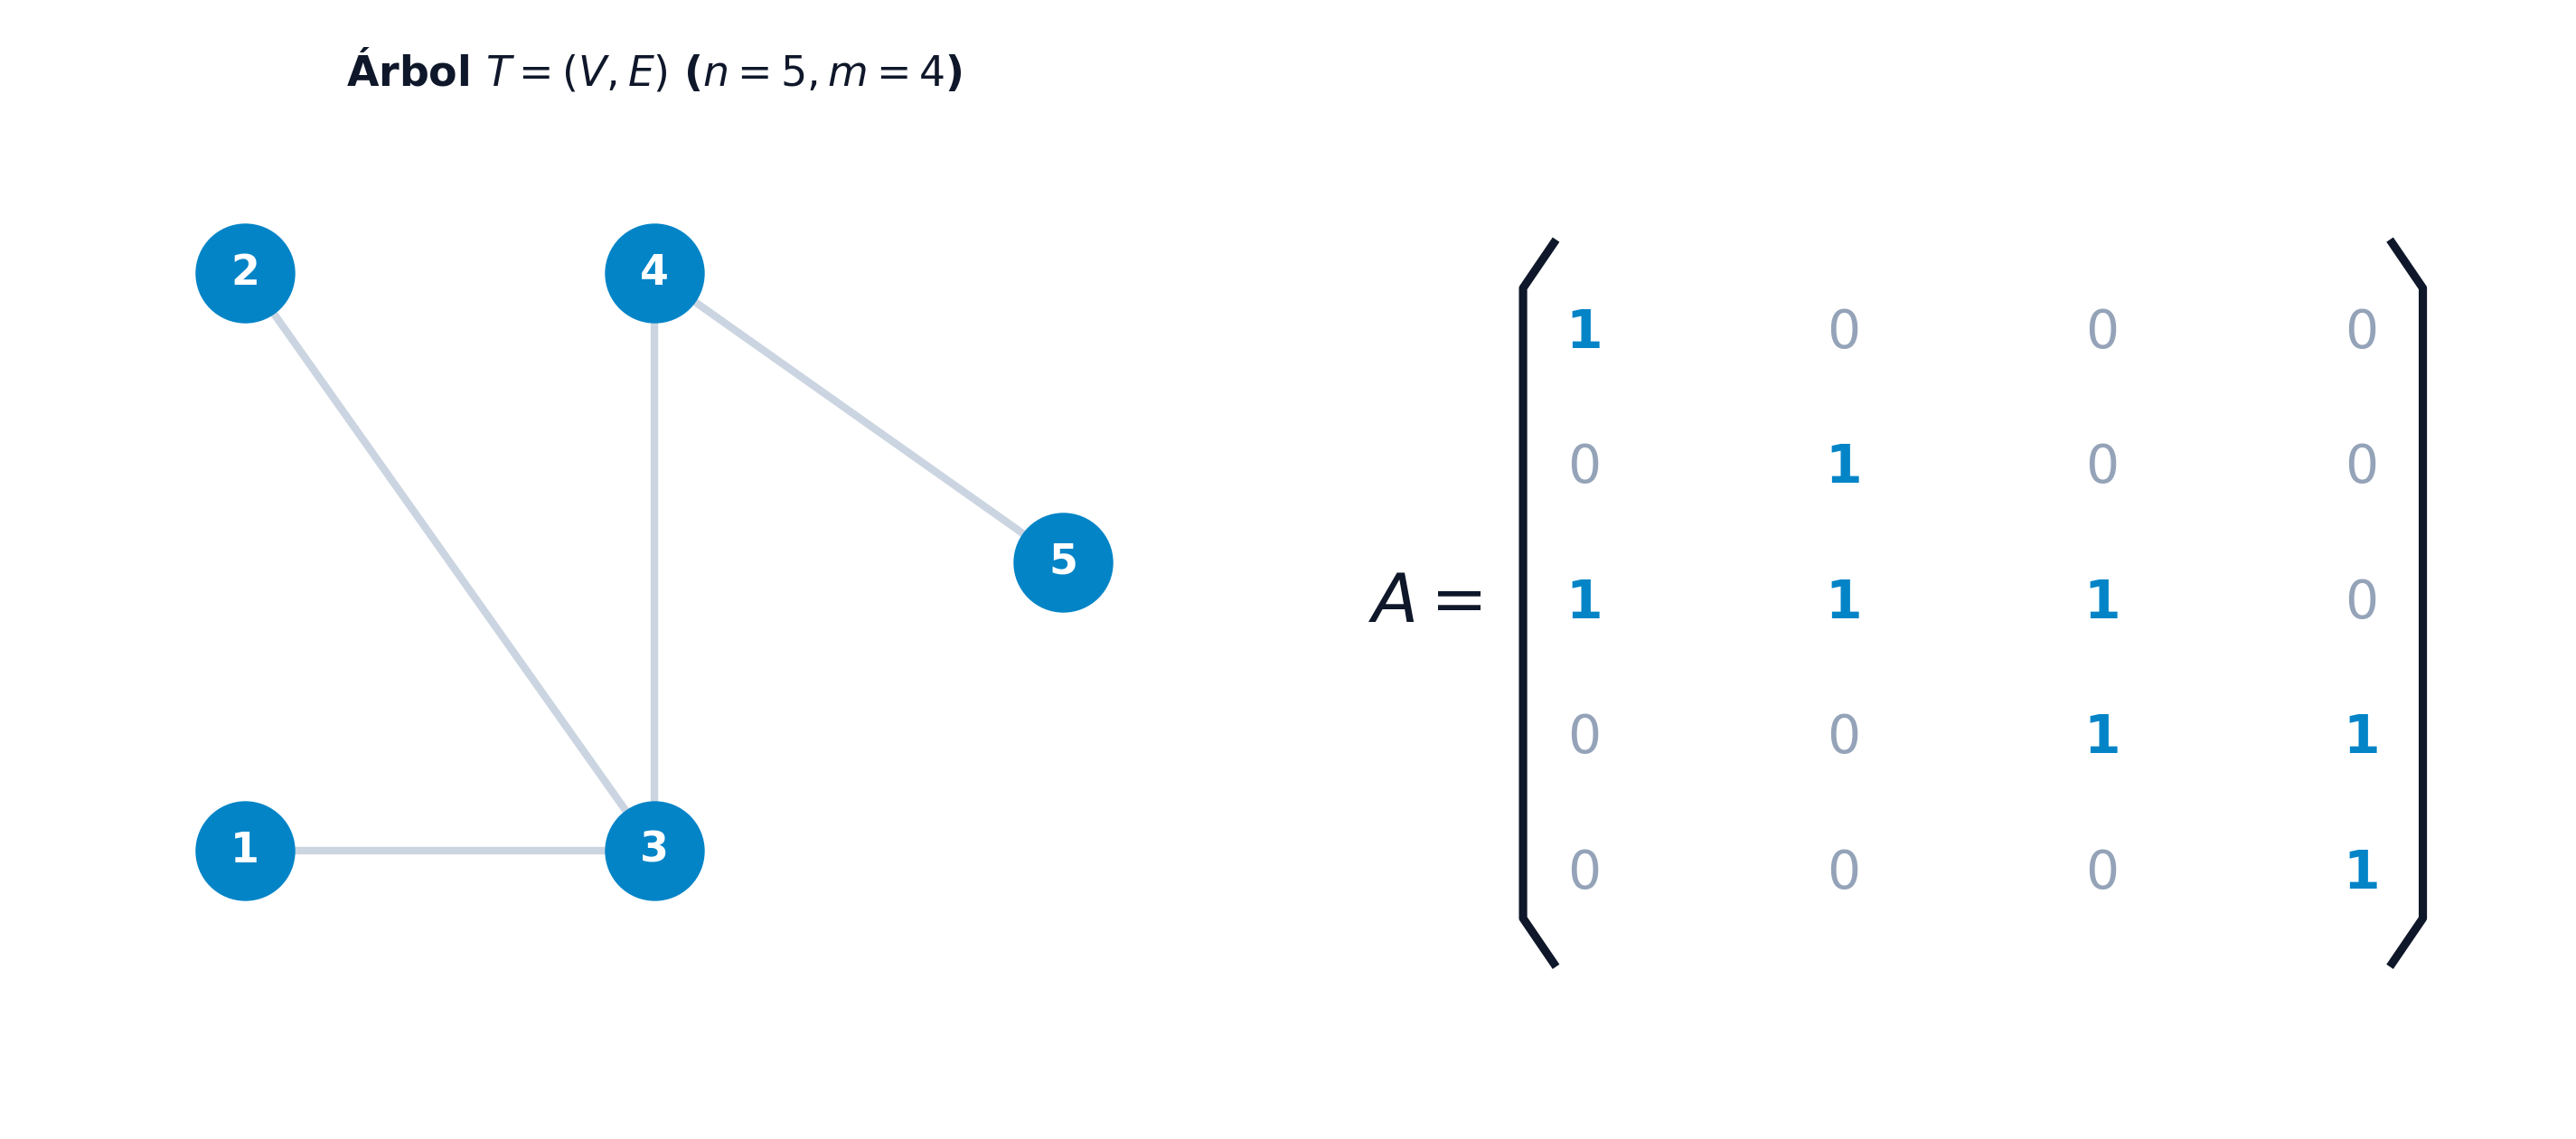
\includegraphics[width=0.85\linewidth,height=\textheight,keepaspectratio]{images/arbol_ejemplo_matriz.png}

}

\caption{\label{fig-arbol-ejemplo-matriz}Ejemplo de un árbol sobre 5
vértices y su correspondiente matriz de incidencia nodo-arista A}

\end{figure}%

La estructura de los árboles presenta múltiples caracterizaciones
algebraicas y geométricas completamente equivalentes entre sí, las
cuales permiten definir a un árbol desde distintos enfoques axiomáticos.

\begin{tcolorbox}[enhanced jigsaw, toprule=.15mm, opacitybacktitle=0.6, coltitle=black, colbacktitle=quarto-callout-important-color!10!white, title=\textcolor{quarto-callout-important-color}{\faExclamation}\hspace{0.5em}{Teorema: Caracterizaciones equivalentes de un árbol}, arc=.35mm, rightrule=.15mm, toptitle=1mm, breakable, bottomtitle=1mm, titlerule=0mm, colback=white, opacityback=0, leftrule=.75mm, colframe=quarto-callout-important-color-frame, left=2mm, bottomrule=.15mm]

\begin{enumerate}
\def\labelenumi{\arabic{enumi}.}
\tightlist
\item
  \(G\) es un \textbf{árbol} (es un grafo conexo y acíclico).
\item
  \(G\) \textbf{no posee ciclos} y si se añade una arista cualquiera
  entre dos vértices no adyacentes, se genera \textbf{un único ciclo}.
\item
  Para todo par de vértices distintos \(x, y \in V\), existe \textbf{una
  única cadena simple} \(\mu[x, y]\) que los conecta.
\item
  \(G\) es \textbf{conexo} y si se elimina una arista cualquiera de
  \(E\), el grafo resultante \textbf{deja de ser conexo} (toda arista de
  un árbol es un puente o arista de corte).
\item
  \(G\) no posee ciclos y tiene exactamente \textbf{\(m = n - 1\)
  aristas}.
\item
  \(G\) es conexo y tiene exactamente \textbf{\(m = n - 1\) aristas}.
\end{enumerate}

\end{tcolorbox}

Este teorema pone de manifiesto que un árbol es una estructura
estrictamente \textbf{crítica y minimal}:

\begin{itemize}
\tightlist
\item
  Es el grafo \textbf{mínimo en aristas que garantiza la conexidad}
  entre los \(n\) vértices (quitar una sola arista desconecta la red).
\item
  Es el grafo \textbf{máximo en aristas que evita la formación de
  ciclos} (añadir una sola arista crea automáticamente un circuito
  cerrado).
\end{itemize}

En el ejemplo de la Figura~\ref{fig-arbol-ejemplo-matriz} se comprueba
inmediatamente esta regla fundamental del recuento de aristas: con
\(n = 5\) vértices, el árbol cuenta con exactamente \(m = 4 = n - 1\)
aristas. Como consecuencia directa, de las tres propiedades básicas de
un grafo sobre \(n\) vértices: (a) ser conexo, (b) ser acíclico y (c)
poseer \(m = n - 1\) aristas, la presencia de \textbf{cualesquiera dos
de ellas implica automáticamente la tercera}, caracterizando de forma
unívoca a la familia de los árboles.

Por último, el número total de árboles soporte etiquetados distintos que
pueden construirse sobre un conjunto dado de \(n\) vértices
diferenciables viene determinado por la célebre \textbf{Fórmula de
Cayley (1889)} (Cayley 1889): \[
T(n) = n^{n-2}
\] Esta fórmula demuestra el crecimiento exponencial combinatorio del
espacio de búsqueda de árboles cuando se evalúan problemas de diseño
topológico en redes de gran escala.

Las propiedades estructurales exclusivas de un árbol, en particular la
existencia de una única cadena simple entre cualquier par de vértices,
permiten comprimir aún más su codificación en memoria, logrando una
\textbf{representación monovectorial} mediante un único vector \(p\) de
dimensión \(n\) (número de vértices).

\begin{tcolorbox}[enhanced jigsaw, toprule=.15mm, opacitybacktitle=0.6, coltitle=black, colbacktitle=quarto-callout-note-color!10!white, title=\textcolor{quarto-callout-note-color}{\faInfo}\hspace{0.5em}{Definición: Representación monovectorial de un árbol (vector de padres o
predecesores)}, arc=.35mm, rightrule=.15mm, toptitle=1mm, breakable, bottomtitle=1mm, titlerule=0mm, colback=white, opacityback=0, leftrule=.75mm, colframe=quarto-callout-note-color-frame, left=2mm, bottomrule=.15mm]

Dado un árbol \(T = (V, E)\) con \(n = |V|\) vértices, al seleccionar de
forma arbitraria un nodo raíz inicial \(x_0 \in V\), la topología de
\(T\) queda unívocamente determinada por el \textbf{vector de padres o
predecesores} \(p \in \mathbb{R}^n\), definido para cada vértice
\(v \in V\) como: \[
p(v) = \begin{cases}
x_0, & \text{si } v = x_0 \text{ (el nodo raíz es su propio padre)}, \\
u, & \text{si } u \in V \text{ es el único antecesor directo de } v \text{ en el camino desde } x_0 \text{ a } v.
\end{cases}
\]

\end{tcolorbox}

Dado que desde el nodo raíz \(x_0\) existe un camino único hacia
cualquier otro vértice \(v \neq x_0\), el antecesor inmediato
\(u = p(v)\) está definido sin ambigüedad. Esta representación
monovectorial resulta extremadamente eficiente en la práctica, pues
almacena la topología de un árbol empleando solo \(n\) enteros en
memoria, frente a los \(O(n + m)\) o matrices \(n \times n\) necesarios
en grafos generales.

La estructura del vector de padres \(p\) depende directamente de la
elección del nodo raíz \(x_0\), adaptando la orientación jerárquica del
árbol. En la Figura~\ref{fig-arbol-vector-padres} se analiza esta
variabilidad sobre el árbol de 5 vértices:

\begin{itemize}
\tightlist
\item
  \textbf{Enraizamiento en \(x_0 = 1\)} (panel izquierdo): La raíz es el
  nodo 1 (\(p(1) = 1\)). El camino desde 1 hasta 5 pasa por el nodo 3
  (\(p(3) = 1\)) y el nodo 4 (\(p(4) = 3\)), de modo que \(p(5) = 4\).
  Los nodos hojas 2 y 4 tienen como padre directo a 3
  (\(p(2) = 3, p(4) = 3\)). El vector de padres resultante es
  \(p = (1, 3, 1, 3, 4)\).
\item
  \textbf{Enraizamiento en \(x_0 = 5\)} (panel derecho): La raíz se
  traslada al nodo 5 (\(p(5) = 5\)). La jerarquía se invierte a lo largo
  del tronco principal: el padre de 4 es 5 (\(p(4) = 5\)), el padre de 3
  es 4 (\(p(3) = 4\)), y los hijos de 3 son 1 y 2
  (\(p(1) = 3, p(2) = 3\)). El vector de padres resultante es
  \(p = (3, 3, 4, 5, 5)\).
\end{itemize}

\begin{figure}

\centering{

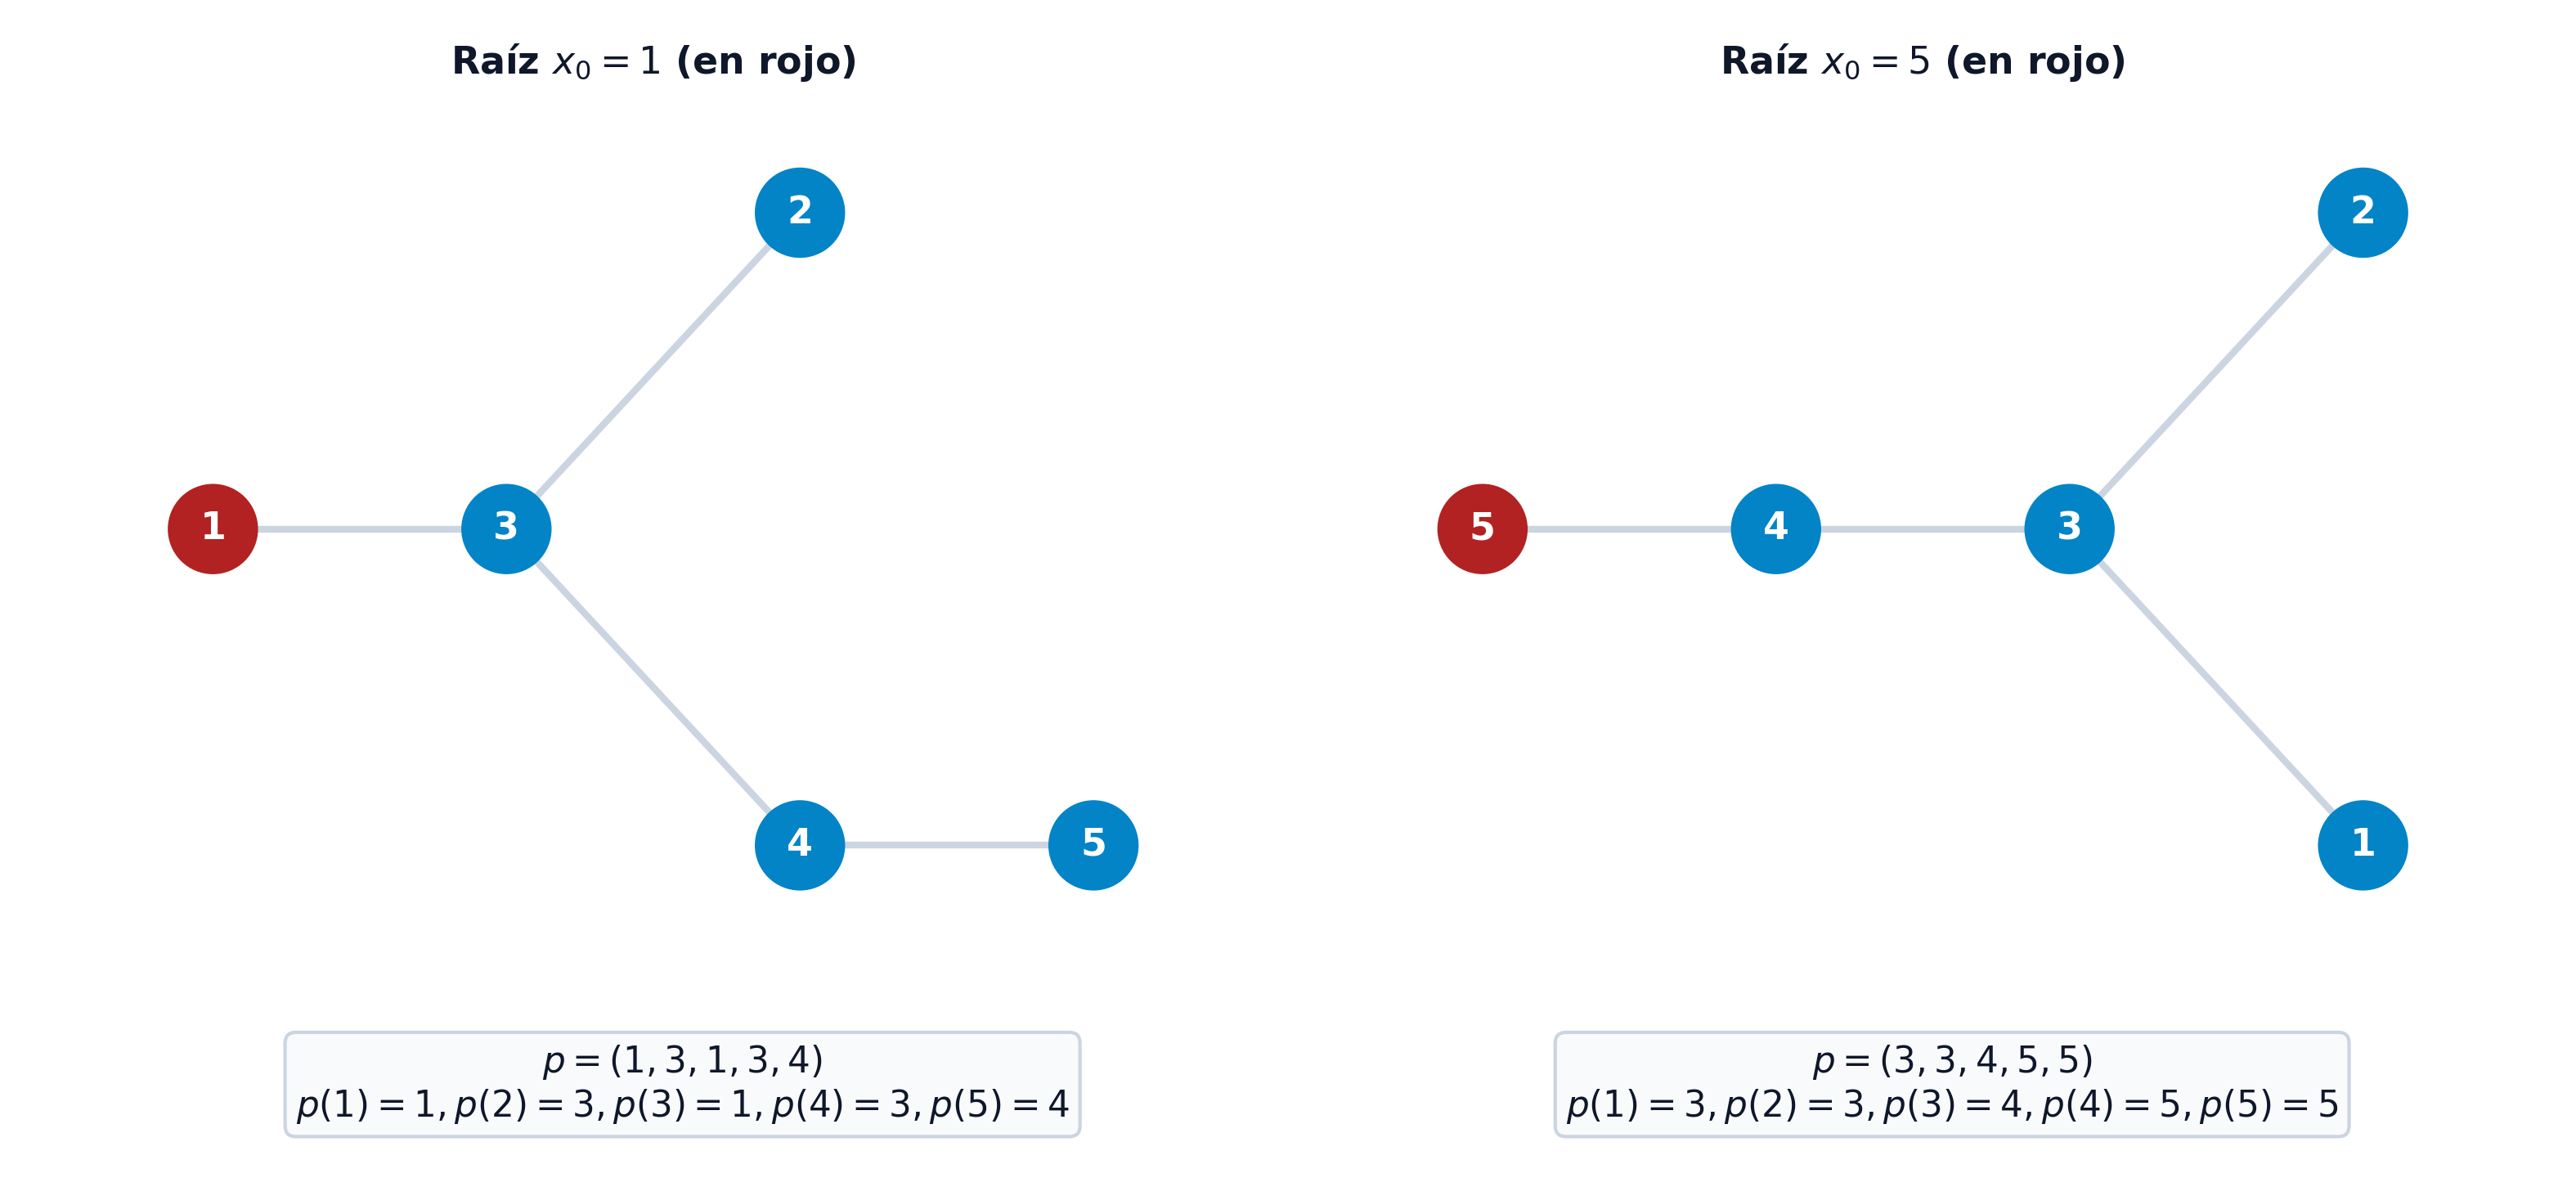
\includegraphics[width=0.9\linewidth,height=\textheight,keepaspectratio]{images/arbol_vector_padres.png}

}

\caption{\label{fig-arbol-vector-padres}Representación monovectorial
mediante el vector de padres p según la elección del nodo raíz x0}

\end{figure}%

\begin{center}\rule{0.5\linewidth}{0.5pt}\end{center}

\section{Árbol soporte de mínimo peso
(MST)}\label{uxe1rbol-soporte-de-muxednimo-peso-mst}

La incorporación de costes, pesos, tiempos o capacidades a las aristas
de un grafo da lugar a la estructura matemática de una \textbf{red
valorada}. En este contexto de optimización, el \textbf{Problema del
Árbol Soporte de Mínimo Peso} (\emph{Minimum Spanning Tree}, MST)
persigue encontrar la infraestructura de conexión de menor coste
acumulado que mantiene la conectividad global entre todos los nodos de
la red sin introducir circuitos cerrados redundantes. Este problema
constituye una de las aplicaciones más emblemáticas de la optimización
combinatoria en el diseño de redes de transporte, distribución
eléctrica, canalización de fluidos y algoritmos de agrupamiento
(\emph{clustering}).

\begin{tcolorbox}[enhanced jigsaw, toprule=.15mm, opacitybacktitle=0.6, coltitle=black, colbacktitle=quarto-callout-note-color!10!white, title=\textcolor{quarto-callout-note-color}{\faInfo}\hspace{0.5em}{Definición: Red valorada y peso total de una arista}, arc=.35mm, rightrule=.15mm, toptitle=1mm, breakable, bottomtitle=1mm, titlerule=0mm, colback=white, opacityback=0, leftrule=.75mm, colframe=quarto-callout-note-color-frame, left=2mm, bottomrule=.15mm]

Una \textbf{red valorada} es un par \((G, \mathbf{d})\), donde
\(G = (V, E)\) o \(G = (V, U)\) es un grafo o digrafo y
\(\mathbf{d} \in \mathbb{R}^m\) es un vector cuyas componentes
identifican el valor numérico, peso o coste \(d(e) = d_e\) asociado a
cada arista \(e \in E\) (o \(c_{ij}\) a cada arco \((i, j) \in U\)). Se
habla de \textbf{red no dirigida} o \textbf{red dirigida} según las
conexiones estén orientadas o no.

\end{tcolorbox}

\begin{tcolorbox}[enhanced jigsaw, toprule=.15mm, opacitybacktitle=0.6, coltitle=black, colbacktitle=quarto-callout-important-color!10!white, title=\textcolor{quarto-callout-important-color}{\faExclamation}\hspace{0.5em}{Formulación primal del problema del árbol soporte de mínimo peso}, arc=.35mm, rightrule=.15mm, toptitle=1mm, breakable, bottomtitle=1mm, titlerule=0mm, colback=white, opacityback=0, leftrule=.75mm, colframe=quarto-callout-important-color-frame, left=2mm, bottomrule=.15mm]

Dada una red no dirigida valorada \((G, \mathbf{d})\) con \(G = (V, E)\)
conexo y valores de peso \(\{d_e : e \in E\}\), el \textbf{Problema del
Árbol Soporte de Mínimo Peso} consiste en encontrar un árbol soporte
\(H = (V, T)\) con \(T \subset E\) que minimice la suma de los pesos de
sus aristas: \[
\begin{aligned}
\min_{T \subset E} \quad & d(T) = \sum_{e \in T} d_e \\
\text{sujeto a} \quad & H = (V, T) \text{ es un árbol soporte de } G
\end{aligned}
\]

\end{tcolorbox}

En la Figura~\ref{fig-mst-ejemplo-tres-arboles} se ilustra el espacio de
soluciones sobre una red no dirigida de 5 vértices
\(V = \{a, b, c, d, e\}\) comparando tres árboles soporte candidatos
alternativos:

\begin{itemize}
\tightlist
\item
  \textbf{Árbol candidato \(T_1\)} (aristas
  \(\{a,b\}, \{a,c\}, \{c,d\}, \{b,e\}\)): Acumula un peso total
  \(d(T_1) = 3 + 2 + 4 + 1 = 10\).
\item
  \textbf{Árbol candidato \(T_2\)} (aristas
  \(\{a,b\}, \{b,c\}, \{b,d\}, \{b,e\}\)): Acumula un peso total
  \(d(T_2) = 3 + 6 + 2 + 1 = 12\).
\item
  \textbf{Árbol mínimo \(T_3\) (Óptimo)} (aristas
  \(\{a,c\}, \{a,b\}, \{b,e\}, \{e,d\}\)): Acumula el peso mínimo
  posible \(d(T_3) = 2 + 3 + 1 + 1 = 7\).
\end{itemize}

\begin{figure}

\centering{

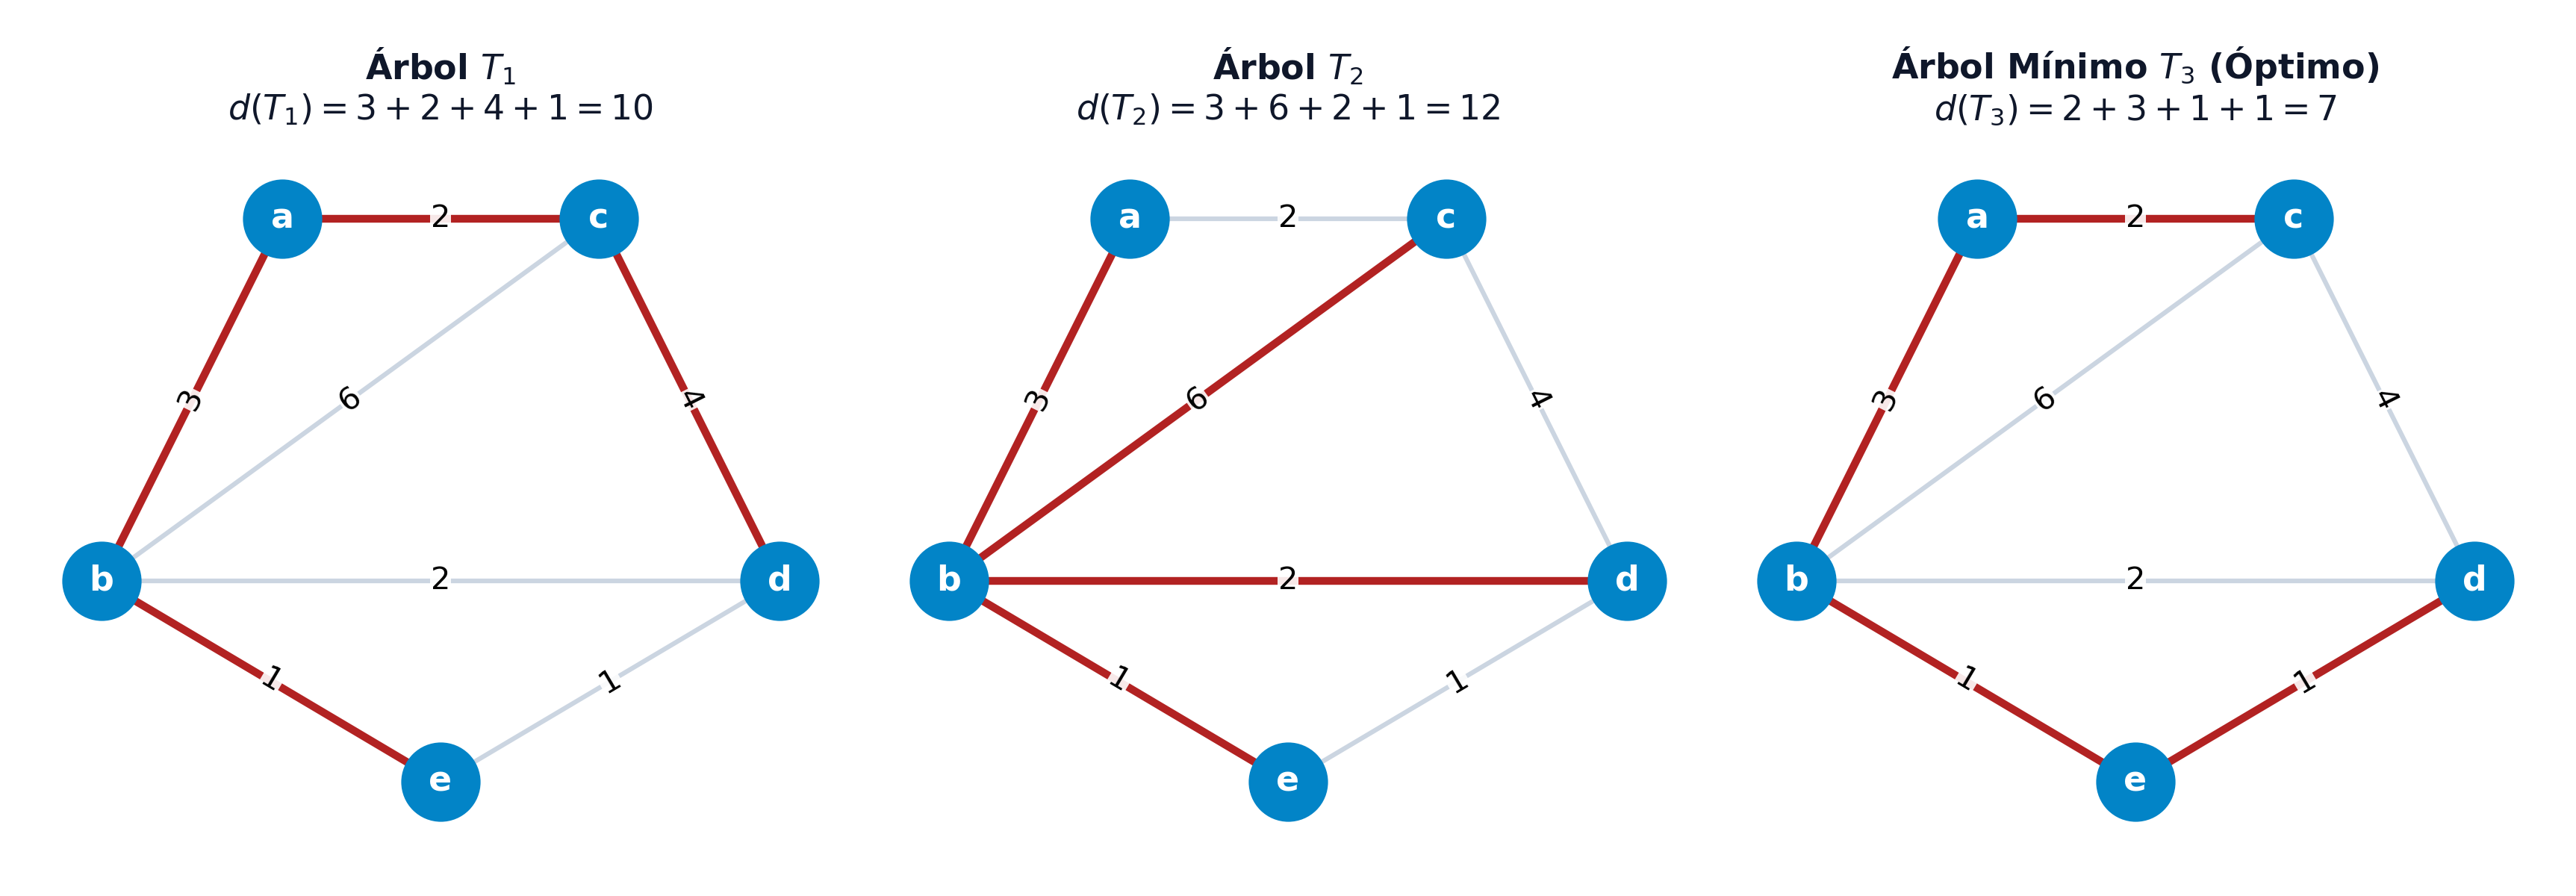
\includegraphics[width=0.9\linewidth,height=\textheight,keepaspectratio]{images/mst_ejemplo_tres_arboles.png}

}

\caption{\label{fig-mst-ejemplo-tres-arboles}Comparación del peso
acumulado en tres árboles soporte candidatos sobre una red no dirigida}

\end{figure}%

Para resolver el problema del árbol soporte de mínimo peso sin necesidad
de evaluar exhaustivamente la cantidad exponencial de árboles soporte
(\(T(n) = n^{n-2}\) por la Fórmula de Cayley), la teoría de grafos se
apoya en una propiedad fundamental de optimalidad local conocida como la
\textbf{Propiedad del Corte}.

\begin{tcolorbox}[enhanced jigsaw, toprule=.15mm, opacitybacktitle=0.6, coltitle=black, colbacktitle=quarto-callout-important-color!10!white, title=\textcolor{quarto-callout-important-color}{\faExclamation}\hspace{0.5em}{Teorema: Propiedad del corte (Cut Property)}, arc=.35mm, rightrule=.15mm, toptitle=1mm, breakable, bottomtitle=1mm, titlerule=0mm, colback=white, opacityback=0, leftrule=.75mm, colframe=quarto-callout-important-color-frame, left=2mm, bottomrule=.15mm]

Sea \((G, \mathbf{d})\) una red valorada conexa no dirigida. Dado
cualquier subconjunto propio de vértices \(S \subset V\), si la arista
\(e^* = \{u, v\}\) con \(u \in S, v \in V \setminus S\) es la arista de
\textbf{peso estrictamente mínimo} que cruza el corte \(w(S)\), entonces
la arista \(e^*\) \textbf{pertenece obligatoriamente a todo Árbol
Soporte de Mínimo Peso} de \(G\).

\end{tcolorbox}

Esta propiedad del corte constituye el fundamento teórico sobre el que
se edifican los dos célebres algoritmos golosos (\emph{greedy}) para la
construcción eficiente del MST: el \textbf{Algoritmo de Kruskal (1956)}
(Kruskal 1956) y el \textbf{Algoritmo de Prim (1957)} (Prim 1957).

\begin{center}\rule{0.5\linewidth}{0.5pt}\end{center}

\subsection{Algoritmo de Kruskal}\label{algoritmo-de-kruskal}

El \textbf{Algoritmo de Kruskal}, propuesto en 1956 por Joseph Kruskal
(Kruskal 1956), adopta un enfoque goloso (\emph{greedy}) centrado en el
ordenamiento global de las aristas. La estrategia fundamental consiste
en examinar secuencialmente las aristas de la red en orden creciente de
peso, e incorporar a la solución parcial la arista de menor coste
disponible, siempre que dicha arista \textbf{no cree un ciclo} con las
aristas ya seleccionadas.

En las fases intermedias del proceso, el conjunto de aristas
seleccionadas \(T\) no forma necesariamente una estructura conexa, sino
un \textbf{bosque parcial de árboles disjuntos} que se van fusionando
paulatinamente hasta formar un único árbol soporte cuando se alcanzan
exactamente \(|T| = n - 1\) aristas.

\begin{tcolorbox}[enhanced jigsaw, toprule=.15mm, opacitybacktitle=0.6, coltitle=black, colbacktitle=quarto-callout-note-color!10!white, title=\textcolor{quarto-callout-note-color}{\faInfo}\hspace{0.5em}{Esquema: Algoritmo de Kruskal}, arc=.35mm, rightrule=.15mm, toptitle=1mm, breakable, bottomtitle=1mm, titlerule=0mm, colback=white, opacityback=0, leftrule=.75mm, colframe=quarto-callout-note-color-frame, left=2mm, bottomrule=.15mm]

Dada una red no dirigida valorada \(G = (V, E, \mathbf{d})\) con
\(n = |V| > 1\) vértices, sin bucles y con pesos \(\{d_e : e \in E\}\):

\begin{itemize}
\item
  \textbf{Paso 0 (Inicialización)}: Definir el conjunto de aristas del
  árbol \(T = \emptyset\) y el conjunto de aristas candidatas
  disponibles \(A \leftarrow E\).
\item
  \textbf{Paso 1 (Bucle de Selección Golosa)}: Mientras \(|T| < n - 1\)
  y \(A \neq \emptyset\):

  \begin{enumerate}
  \def\labelenumi{\arabic{enumi}.}
  \tightlist
  \item
    Identificar la arista de menor peso \(e \in A\).
  \item
    Actualizar el conjunto de disponibles:
    \(A \leftarrow A \setminus \{e\}\).
  \item
    Si el subconjunto \(T \cup \{e\}\) \textbf{no contiene ningún
    ciclo}, aceptar la arista: \(T \leftarrow T \cup \{e\}\).
  \end{enumerate}
\item
  \textbf{Paso 2 (Criterio de Parada y Verificación)}:

  \begin{itemize}
  \tightlist
  \item
    Si \(|T| = n - 1\), el par \(H = (V, T)\) es el \textbf{Árbol
    Soporte de Mínimo Peso (MST)}.
  \item
    Si \(A = \emptyset\) y \(|T| < n - 1\), la red \(G\) no era conexa,
    obteniéndose el bosque soporte de mínimo peso de sus componentes.
  \end{itemize}
\end{itemize}

\end{tcolorbox}

Para implementar el algoritmo con la máxima eficiencia computacional, la
verificación de si una arista candidata \(e = \{i, j\}\) forma un ciclo
en \(T\) no requiere explorar la red completa, sino utilizar la
estructura de datos de \textbf{conjuntos disjuntos} (\emph{Union-Find}):

\begin{itemize}
\tightlist
\item
  Inicialmente, cada uno de los \(n\) vértices constituye su propia
  componente disjunta independiente: \(S_k = \{k\}\) para todo
  \(k \in V\).
\item
  Al evaluar una arista \(e = \{i, j\}\), se consulta el identificador
  de subconjunto al que pertenecen sus extremos mediante la operación
  \(\text{Find}(i)\) y \(\text{Find}(j)\).
\item
  Si \(\text{Find}(i) \neq \text{Find}(j)\), los vértices pertenecen a
  componentes distintas, garantizando que la incorporación de
  \(\{i, j\}\) \textbf{no genera ningún ciclo}. En tal caso, la arista
  se añade a \(T\) y se unen ambas componentes mediante la operación
  \(\text{Union}(S(i), S(j))\).
\item
  Si \(\text{Find}(i) = \text{Find}(j)\), ambos vértices ya estaban
  conectados previamente a través de otras aristas de \(T\), por lo que
  \(\{i, j\}\) se descarta por formar un ciclo cerrado redundante.
\end{itemize}

Adicionalmente, se pueden eliminar de forma anticipada de \(A\) todas
las aristas restantes que unan vértices que ya pertenezcan al mismo
subconjunto disjunto.

\begin{tcolorbox}[enhanced jigsaw, toprule=.15mm, opacitybacktitle=0.6, coltitle=black, colbacktitle=quarto-callout-tip-color!10!white, title=\textcolor{quarto-callout-tip-color}{\faLightbulb}\hspace{0.5em}{Ejemplo: Aplicación del algoritmo de Kruskal}, arc=.35mm, rightrule=.15mm, toptitle=1mm, breakable, bottomtitle=1mm, titlerule=0mm, colback=white, opacityback=0, leftrule=.75mm, colframe=quarto-callout-tip-color-frame, left=2mm, bottomrule=.15mm]

\textbf{Obtener el árbol de expansión de peso mínimo mediante el
Algoritmo de Kruskal para la red no dirigida sobre \(n = 6\) vértices
presentada en la Figura~\ref{fig-kruskal-ejemplo-matriz}.}

\textbf{Planteamiento e Inicialización}: La red no dirigida
\(G = (V, E)\) está compuesta por 6 vértices
\(V = \{1, 2, 3, 4, 5, 6\}\) y 11 aristas valoradas. Su topología y su
correspondiente matriz simétrica de pesos
\(B \in \mathbb{R}^{6 \times 6}\) se detallan en la
Figura~\ref{fig-kruskal-ejemplo-matriz}.

\begin{figure}[H]

\centering{

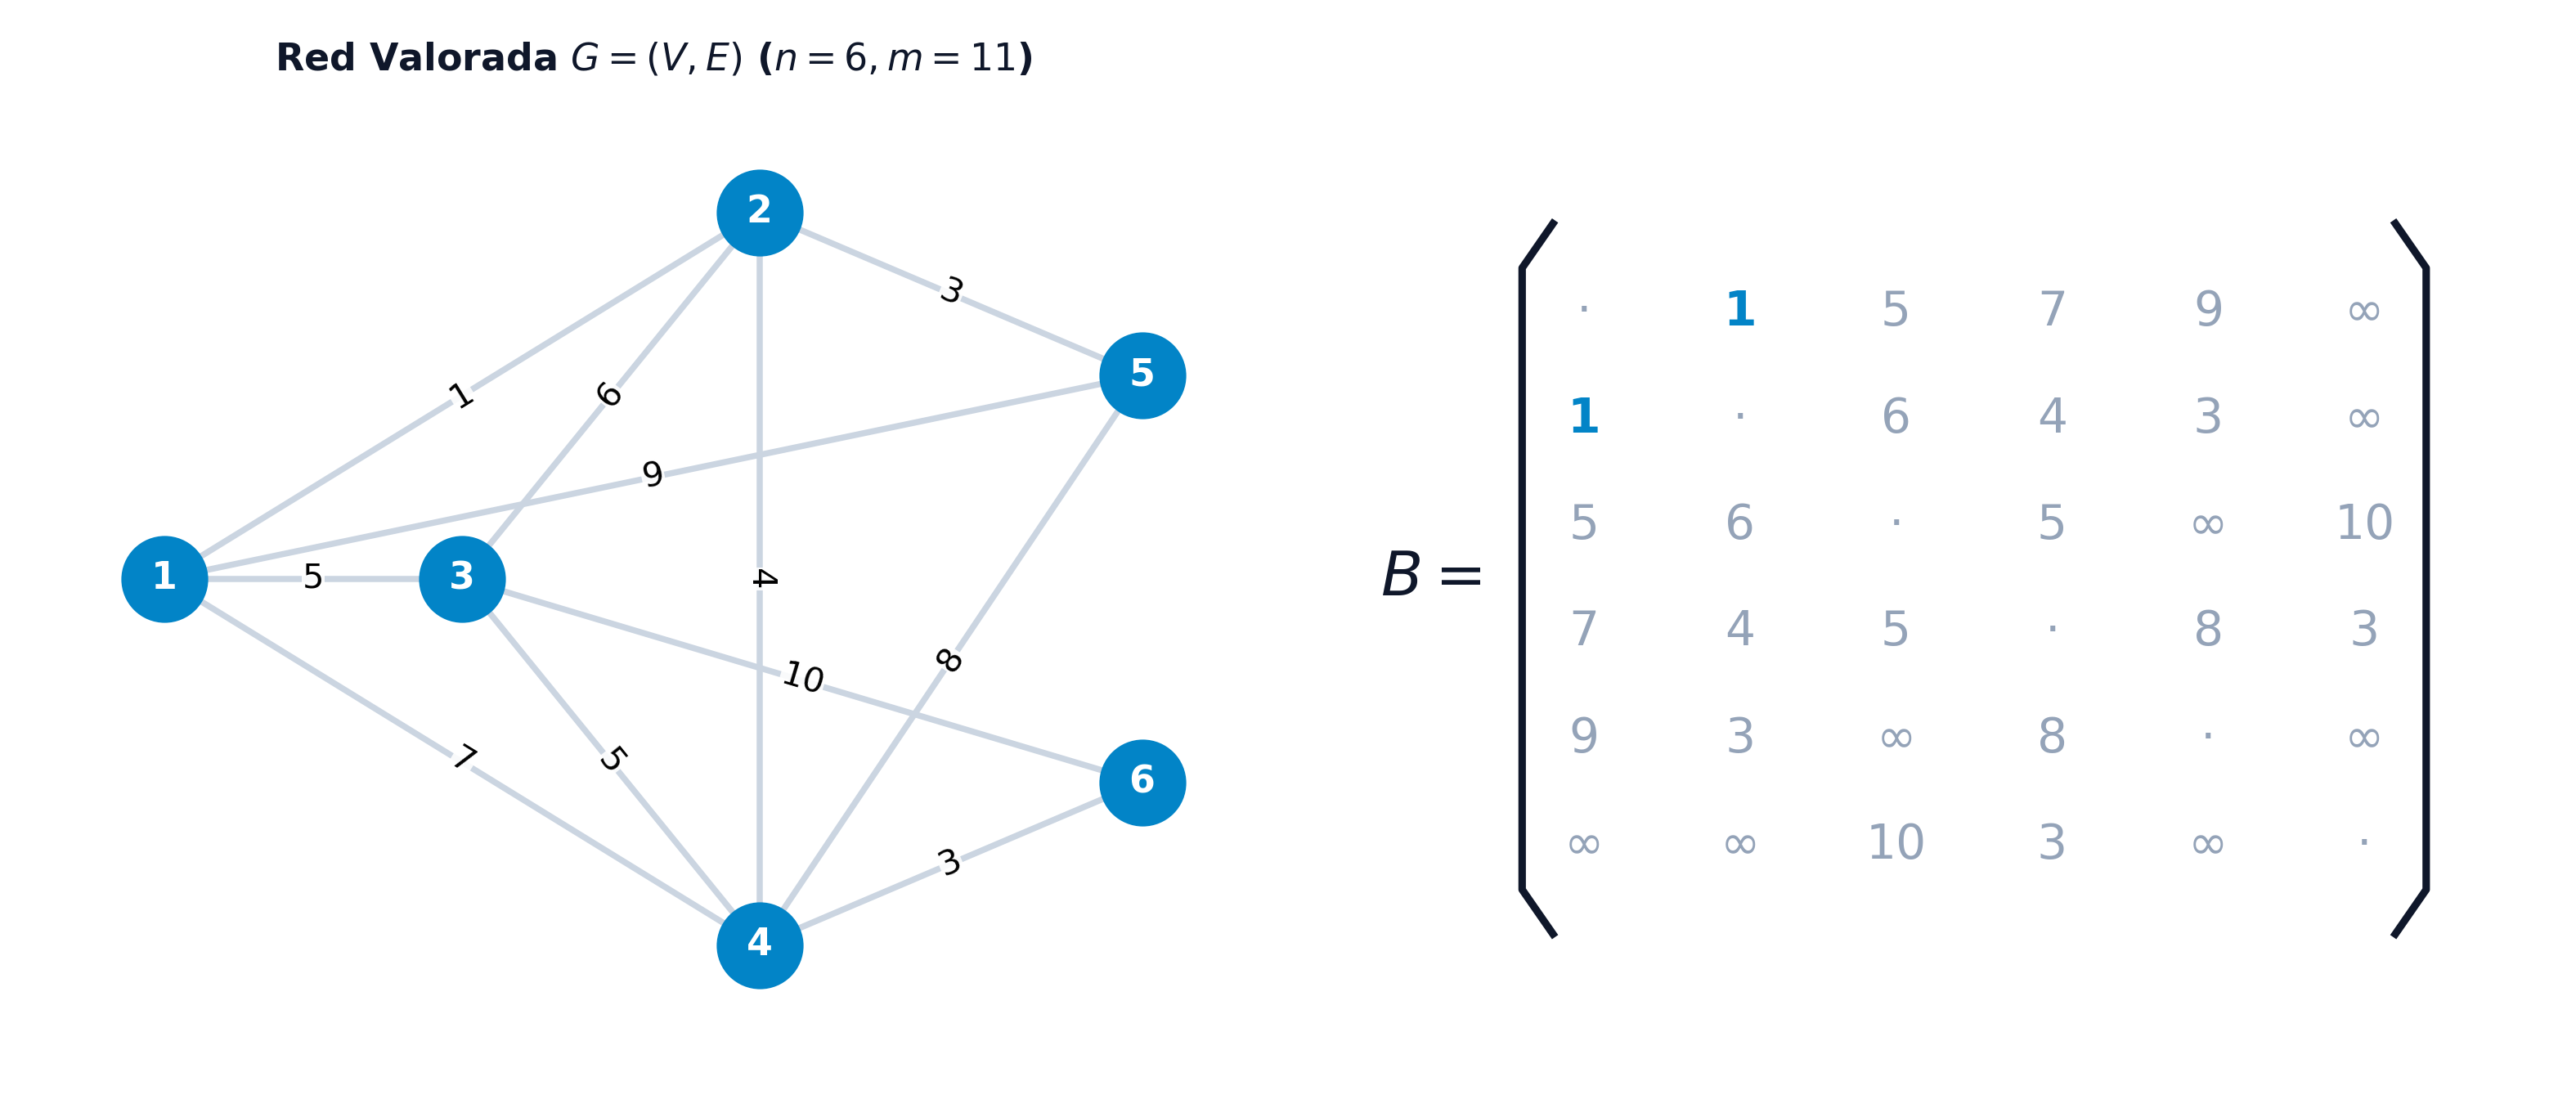
\includegraphics[width=0.9\linewidth,height=\textheight,keepaspectratio]{images/kruskal_ejemplo_matriz.png}

}

\caption{\label{fig-kruskal-ejemplo-matriz}Red no dirigida de 6 vértices
y su correspondiente matriz simétrica de pesos B}

\end{figure}%

En el estado inicial (\(k=0\)):

\begin{itemize}
\tightlist
\item
  El árbol parcial solución se encuentra vacío: \(T = \emptyset\).
\item
  Cada vértice pertenece a su propio subconjunto disjunto independiente:
  \[
  \{1\}, \, \{2\}, \, \{3\}, \, \{4\}, \, \{5\}, \, \{6\}
  \]
\end{itemize}

\textbf{Resolución Iterativa Paso a Paso}:

\begin{enumerate}
\def\labelenumi{\arabic{enumi}.}
\item
  \textbf{Iteración \(k=1\) (peso mínimo \(d = 1\))}: Se selecciona la
  arista de menor peso global \(e_1 = \{1, 2\}\) con
  \(d_{\{1,2\}} = 1\). Dado que los nodos 1 y 2 pertenecen a componentes
  distintas (\(\text{Find}(1) \neq \text{Find}(2)\)), se acepta la
  arista en \(T\) y se fusionan sus subconjuntos:

  \begin{itemize}
  \tightlist
  \item
    Árbol parcial: \(T = \{\{1, 2\}\}\).
  \item
    Componentes disjuntas:
    \(\{1, 2\}, \, \{3\}, \, \{4\}, \, \{5\}, \, \{6\}\).
  \end{itemize}
\item
  \textbf{Iteración \(k=2\) (peso mínimo \(d = 3\), resolución de
  empate)}: Las aristas no seleccionadas de menor peso son \(\{2, 5\}\)
  y \(\{4, 6\}\), ambas de peso 3. Se selecciona la arista \(\{2, 5\}\).
  Como 5 no pertenece a la componente de 2 (\(\{1, 2\} \neq \{5\}\)), se
  acepta la arista:

  \begin{itemize}
  \tightlist
  \item
    Árbol parcial: \(T = \{\{1, 2\}, \{2, 5\}\}\).
  \item
    Componentes disjuntas:
    \(\{1, 2, 5\}, \, \{3\}, \, \{4\}, \, \{6\}\).
  \end{itemize}
\item
  \textbf{Iteración \(k=3\) (peso mínimo \(d = 3\))}: Se selecciona la
  arista disponible \(\{4, 6\}\) de peso 3. Puesto que
  \(\text{Find}(4) \neq \text{Find}(6)\), la arista no forma ciclos y se
  incorpora a la solución:

  \begin{itemize}
  \tightlist
  \item
    Árbol parcial: \(T = \{\{1, 2\}, \{2, 5\}, \{4, 6\}\}\).
  \item
    Componentes disjuntas: \(\{1, 2, 5\}, \, \{3\}, \, \{4, 6\}\).
  \end{itemize}
\item
  \textbf{Iteración \(k=4\) (peso mínimo \(d = 4\))}: La arista
  candidata de menor peso es \(\{2, 4\}\) con peso 4. Dado que el nodo 2
  pertenece al bloque \(\{1, 2, 5\}\) y el nodo 4 pertenece al bloque
  \(\{4, 6\}\), ambas componentes son distintas y la arista no genera
  ciclos. Se acepta \(\{2, 4\}\) y se fusionan ambos bloques:

  \begin{itemize}
  \tightlist
  \item
    Árbol parcial: \(T = \{\{1, 2\}, \{2, 5\}, \{4, 6\}, \{2, 4\}\}\).
  \item
    Componentes disjuntas: \(\{1, 2, 4, 5, 6\}, \, \{3\}\).
  \end{itemize}
\item
  \textbf{Iteración \(k=5\) (peso mínimo \(d = 5\), resolución de empate
  final)}: Las aristas disponibles de menor peso son \(\{1, 3\}\) y
  \(\{3, 4\}\), ambas de peso 5. Se selecciona la arista \(\{1, 3\}\).
  Puesto que el nodo 3 se encuentra en la componente aislada \(\{3\}\) y
  el nodo 1 está en el bloque principal \(\{1, 2, 4, 5, 6\}\), la arista
  se acepta y se logra la conectividad total de la red:

  \begin{itemize}
  \tightlist
  \item
    Árbol parcial final:
    \(T = \{\{1, 2\}, \{2, 5\}, \{4, 6\}, \{2, 4\}, \{1, 3\}\}\).
  \item
    Componentes disjuntas final: \(\{1, 2, 3, 4, 5, 6\}\) (1 sola
    componente conexa).
  \end{itemize}
\end{enumerate}

En la Figura~\ref{fig-kruskal-ejemplo-pasos} se ilustra la evolución
gráfica de la construcción progresiva del árbol paso a paso a lo largo
de las 5 iteraciones.

\begin{figure}[H]

\centering{

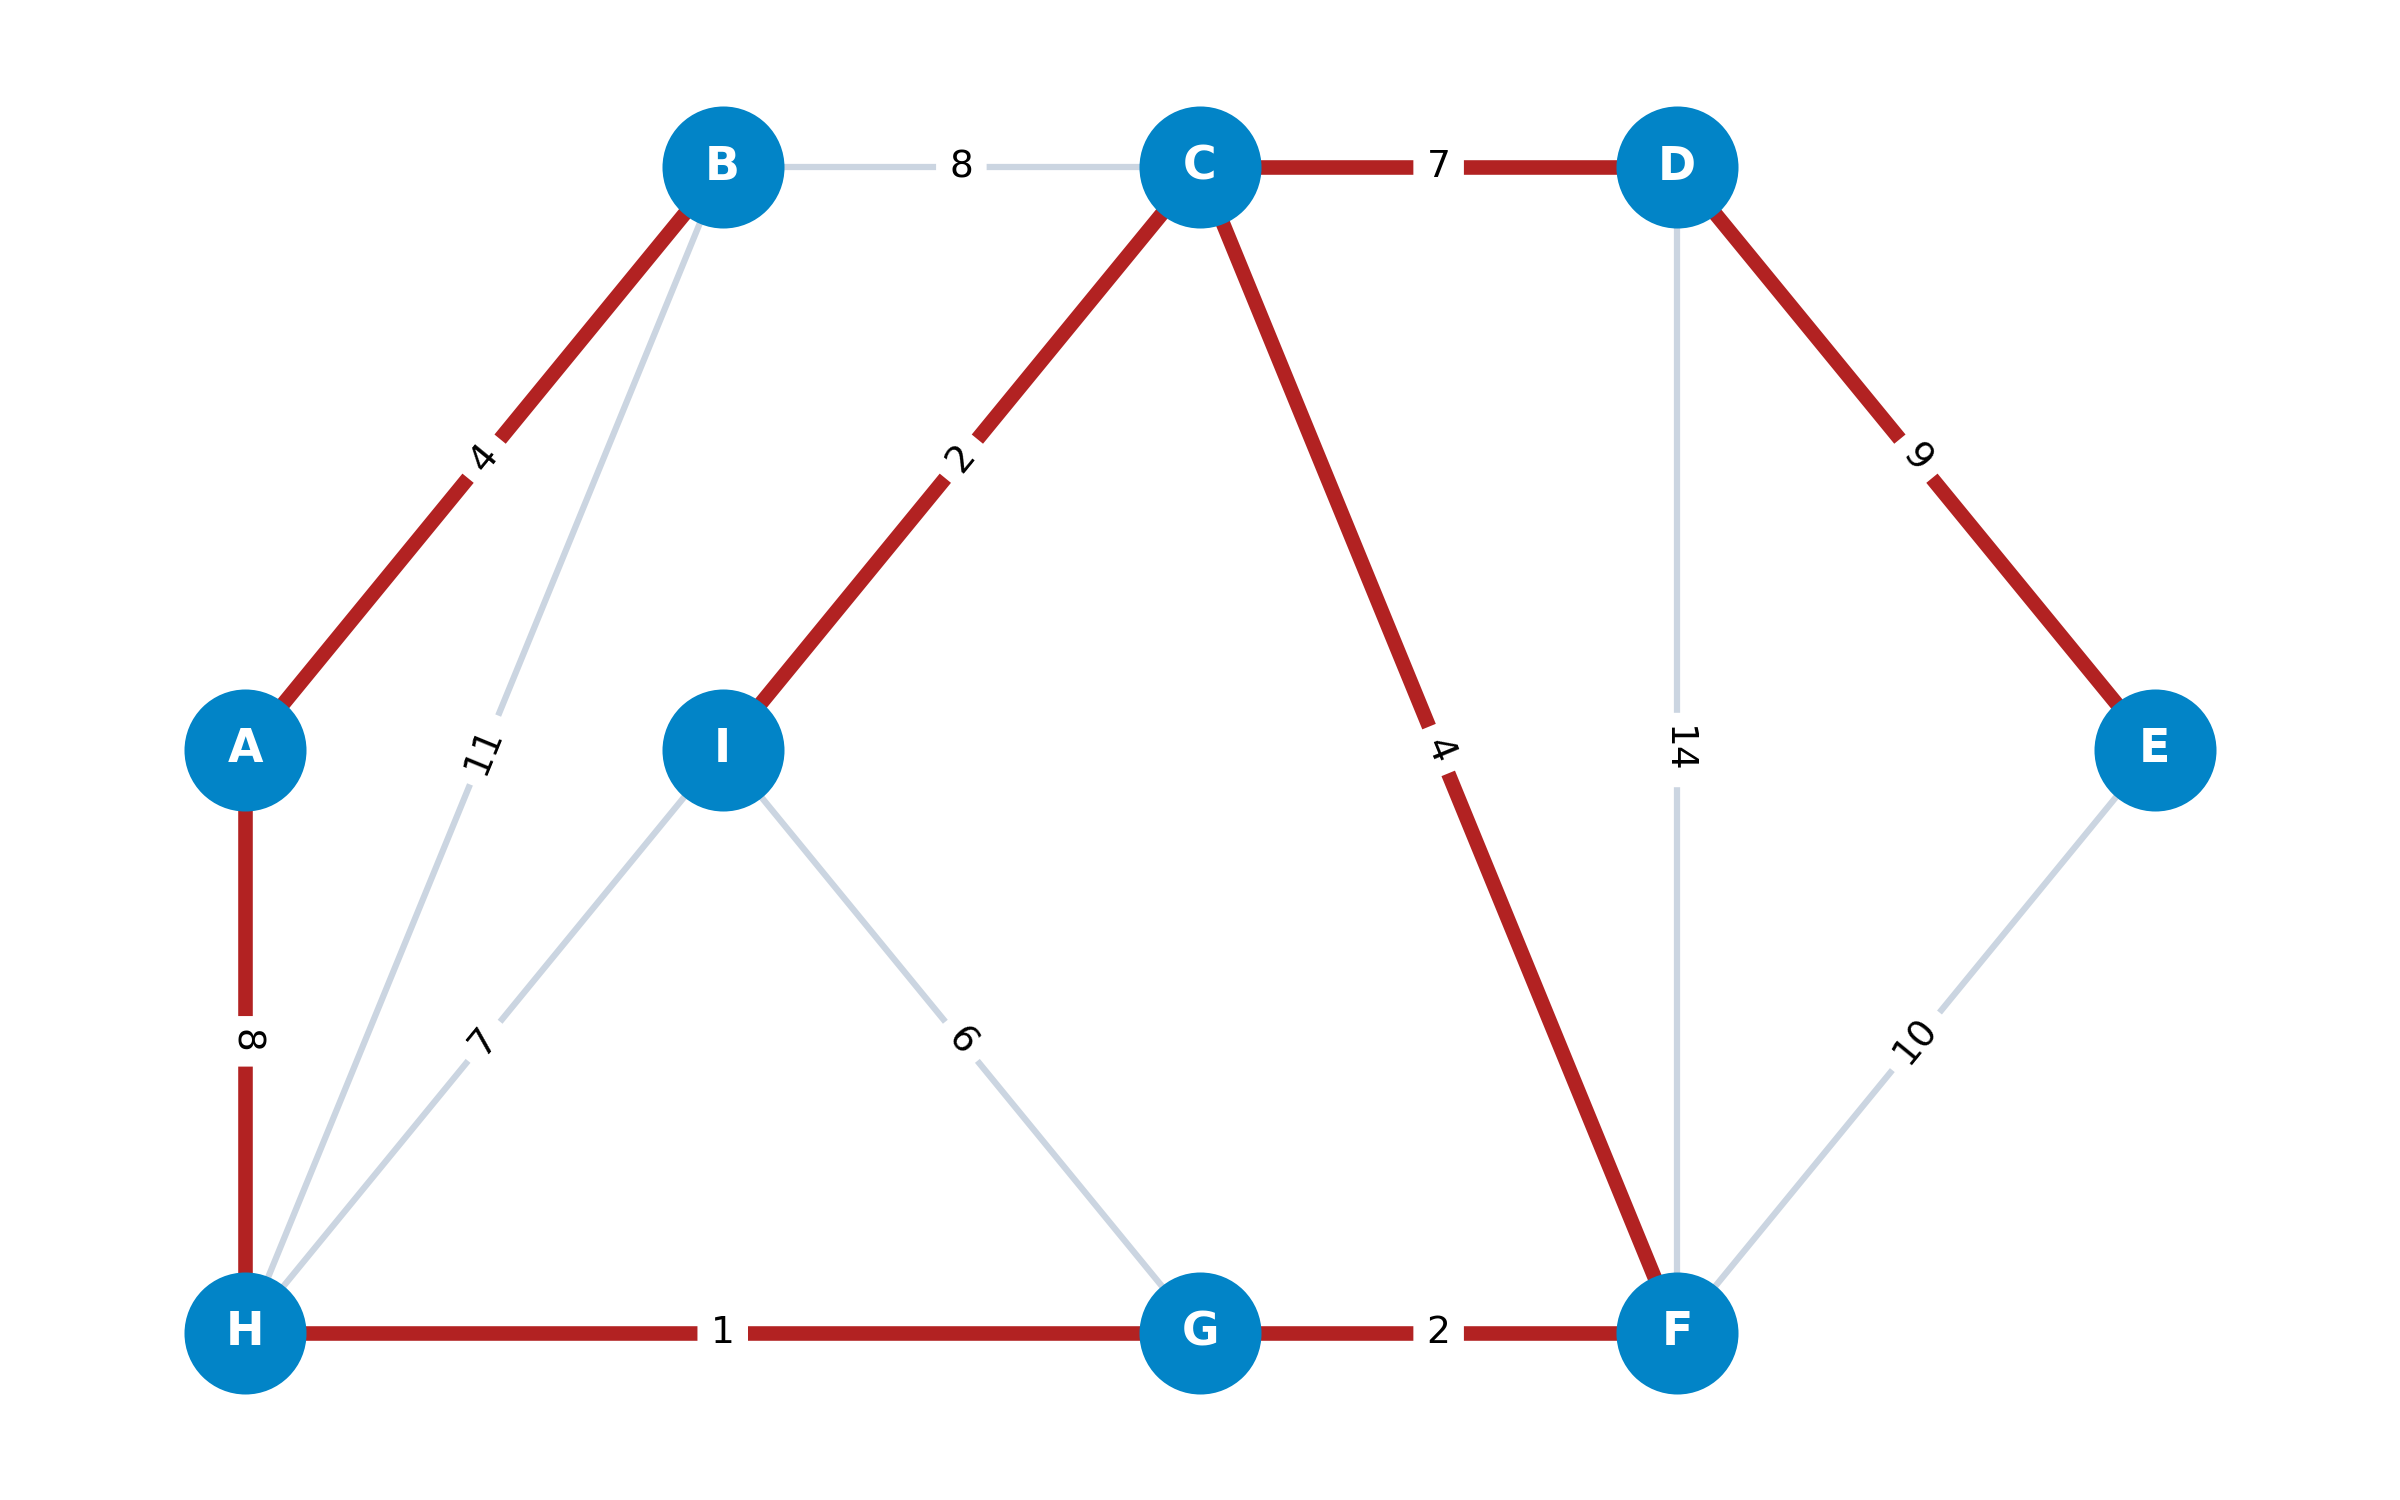
\includegraphics[width=0.75\linewidth,height=\textheight,keepaspectratio]{images/kruskal_traza_paso_a_paso.png}

}

\caption{\label{fig-kruskal-ejemplo-pasos}Traza gráfica de la evolución
iterativa del Algoritmo de Kruskal paso a paso}

\end{figure}%

\textbf{Conclusión y Peso del Árbol Soporte de Mínimo Peso}: Al
alcanzarse \(|T| = n - 1 = 5\) aristas, el algoritmo finaliza. El árbol
soporte de mínimo peso \(H = (V, T)\) acumula un peso total óptimo de:
\[
d(T) = d_{\{1,2\}} + d_{\{2,5\}} + d_{\{4,6\}} + d_{\{2,4\}} + d_{\{1,3\}} = 1 + 3 + 3 + 4 + 5 = 16
\]

\textbf{Observación sobre la No Unicidad de la Solución}: Puesto que en
la iteración \(k=5\) existía un empate de peso mínimo (\(d=5\)) entre
las aristas \(\{1, 3\}\) y \(\{3, 4\}\), si en lugar de seleccionar
\(\{1, 3\}\) se hubiera optado por incorporar \(\{3, 4\}\), se obtendría
un \textbf{árbol soporte de mínimo peso alternativo}: \[
T' = \{\{1, 2\}, \{2, 5\}, \{4, 6\}, \{2, 4\}, \{3, 4\}\}
\] El peso acumulado en esta solución alternativa es
\(d(T') = 1 + 3 + 3 + 4 + 5 = 16\), idéntico al del árbol \(T\). Esto
demuestra que cuando una red contiene aristas con pesos repetidos, el
árbol soporte de mínimo peso \textbf{no es necesariamente único}, aunque
el valor del peso óptimo \(d(T)\) permanezca siempre constante e
invariable.

\end{tcolorbox}

\begin{tcolorbox}[enhanced jigsaw, toprule=.15mm, opacitybacktitle=0.6, coltitle=black, colbacktitle=quarto-callout-important-color!10!white, title=\textcolor{quarto-callout-important-color}{\faExclamation}\hspace{0.5em}{Teorema: Correctitud del algoritmo de Kruskal}, arc=.35mm, rightrule=.15mm, toptitle=1mm, breakable, bottomtitle=1mm, titlerule=0mm, colback=white, opacityback=0, leftrule=.75mm, colframe=quarto-callout-important-color-frame, left=2mm, bottomrule=.15mm]

Dada una red conexa valorada \((G, \mathbf{d})\), el conjunto de aristas
\(T\) construido secuencialmente por el Algoritmo de Kruskal constituye
un \textbf{Árbol Soporte de Mínimo Peso} del grafo \(G\).

\emph{Demostración}: La correctitud del procedimiento se deriva
directamente de la Propiedad del Corte. En cada paso \(k\), la arista
seleccionada \(e = \{u, v\}\) es la de peso estrictamente mínimo entre
todas las aristas disponibles que unen la componente disjunta \(S(u)\)
con el resto de la red \(V \setminus S(u)\). Por consiguiente, por el
Teorema de la Propiedad del Corte, la arista \(e\) pertenece
obligatoriamente a un árbol soporte de mínimo peso, garantizando la
optimalidad global del árbol resultante al finalizar las \(n - 1\)
iteraciones.

\end{tcolorbox}

\textbf{Complejidad Computacional}: La eficiencia del Algoritmo de
Kruskal depende fundamentalmente de la etapa de ordenación previa de las
aristas y del rendimiento de la estructura de datos \emph{Union-Find}:

\begin{itemize}
\item
  \textbf{Aristas preordenadas}: Si la colección de \(m\) aristas ya se
  encuentra clasificada por orden de peso, el bucle principal realiza a
  lo sumo \(m\) operaciones \(\text{Find}\) y \(n - 1\) operaciones
  \(\text{Union}\). Empleando la estructura \emph{Union-Find} optimizada
  con compresión de caminos y unión por rango, la complejidad resultante
  es \(O(m \cdot \alpha(n))\), donde \(\alpha(n)\) es la inversa de la
  función de Ackermann (efectivamente \(O(m \cdot n)\) en cotas
  elementales o casi lineal en la práctica).
\item
  \textbf{Caso general sin ordenación previa}: Cuando las aristas no
  están clasificadas, el coste computacional dominante viene determinado
  por el algoritmo de ordenación (como \emph{Heapsort} o
  \emph{Quicksort}), que requiere un tiempo de \(O(m \log m)\). Puesto
  que en cualquier grafo simple \(m \le n^2\) y por tanto
  \(\log m \le 2 \log n\), la complejidad temporal total del Algoritmo
  de Kruskal se establece en \textbf{\(O(m \log m)\)} o equivalentemente
  \textbf{\(O(m \log n)\)}.
\end{itemize}

\begin{center}\rule{0.5\linewidth}{0.5pt}\end{center}

\subsection{Algoritmo de Prim}\label{algoritmo-de-prim}

El \textbf{Algoritmo de Prim} fue publicado en 1957 por Robert C. Prim
(Prim 1957). No obstante, este procedimiento fue descubierto
inicialmente por el matemático checo Vojtěch Jarník en 1930 (Jarnı́k
1930) y posteriormente redescubierto de forma independiente por Edsger
W. Dijkstra en 1959 (Dijkstra 1959). Por esta razón, en la literatura
científica especializada se le conoce formalmente como el
\textbf{Algoritmo de Jarník-Prim-Dijkstra}.

A diferencia del Algoritmo de Kruskal (que evalúa aristas globales
formando un bosque inconexo en sus fases intermedias), el Algoritmo de
Prim construye el árbol soporte de mínimo peso haciendo crecer
\textbf{una única componente conexa continua} (o arborescencia) a partir
de un nodo raíz inicial \(v_1 \in V\) elegido de forma arbitraria.

Sea \(P \subset V\) el conjunto de vértices ya integrados en la solución
parcial (inicialmente \(P = \{v_1\}\)) y \(N = V \setminus P\) el
conjunto de nodos pendientes de visitar. En cada iteración, el algoritmo
analiza las aristas del corte \(w(P)\) que conectan el conjunto \(P\)
con los nodos de \(N\). A continuación, aplica directamente la
\textbf{Propiedad del Corte}, seleccionando la arista
\(e^* = \{x^*, y^*\}\) (con \(x^* \in P\) y \(y^* \in N\)) de peso
estrictamente mínimo, incorporando el nuevo vértice \(y^*\) al
subconjunto \(P\).

\begin{tcolorbox}[enhanced jigsaw, toprule=.15mm, opacitybacktitle=0.6, coltitle=black, colbacktitle=quarto-callout-note-color!10!white, title=\textcolor{quarto-callout-note-color}{\faInfo}\hspace{0.5em}{Esquema: Algoritmo de Prim}, arc=.35mm, rightrule=.15mm, toptitle=1mm, breakable, bottomtitle=1mm, titlerule=0mm, colback=white, opacityback=0, leftrule=.75mm, colframe=quarto-callout-note-color-frame, left=2mm, bottomrule=.15mm]

Dada una red no dirigida valorada \(G = (V, E, \mathbf{d})\) conexa con
\(n = |V| > 1\) vértices, sin bucles y con pesos de arista
\(\{d_e : e \in E\}\):

\begin{itemize}
\item
  \textbf{Paso 0 (Inicialización)}:

  \begin{enumerate}
  \def\labelenumi{\arabic{enumi}.}
  \tightlist
  \item
    Seleccionar un nodo raíz inicial \(v_1 \in V\) de manera arbitraria.
  \item
    Inicializar el conjunto de nodos visitados \(P = \{v_1\}\) y el de
    no visitados \(N = V \setminus \{v_1\}\).
  \item
    Inicializar el conjunto de aristas del árbol \(T = \emptyset\) y el
    contador de iteraciones \(i = 1\).
  \end{enumerate}
\item
  \textbf{Paso 1 (Selección de la Arista Mínima del Corte)}:

  \begin{itemize}
  \item
    Identificar la arista \(e^* = \{x^*, y^*\} \in E\) tal que
    \(x^* \in P, y^* \in N\) que minimice el peso \(d(e^*)\): \[
    d(e^*) = \min \{d(e) : e = \{x, y\}, x \in P, y \in N\}
    \]
  \item
    \textbf{Criterio de Conexidad}:

    \begin{itemize}
    \tightlist
    \item
      Si \(d(e^*) = \infty\) (no existen aristas que crucen el corte
      \(w(P)\)), detener el proceso: la red \(G\) no es conexa.
    \item
      Si \(d(e^*) < \infty\), actualizar los conjuntos: \[
      P \leftarrow P \cup \{y^*\}, \quad N \leftarrow N \setminus \{y^*\}, \quad T \leftarrow T \cup \{e^*\}
      \]
    \end{itemize}
  \end{itemize}
\item
  \textbf{Paso 2 (Criterio de Parada e Incremento)}:

  \begin{itemize}
  \tightlist
  \item
    Si \(i = n - 1\), detener el procedimiento: el par \(H = (V, T)\) es
    un \textbf{Árbol Soporte de Mínimo Peso (MST)}.
  \item
    Si \(i < n - 1\), actualizar \(i \leftarrow i + 1\) y regresar al
    Paso 1.
  \end{itemize}
\end{itemize}

\end{tcolorbox}

\begin{tcolorbox}[enhanced jigsaw, toprule=.15mm, opacitybacktitle=0.6, coltitle=black, colbacktitle=quarto-callout-tip-color!10!white, title=\textcolor{quarto-callout-tip-color}{\faLightbulb}\hspace{0.5em}{Ejemplo: Aplicación del algoritmo de Prim}, arc=.35mm, rightrule=.15mm, toptitle=1mm, breakable, bottomtitle=1mm, titlerule=0mm, colback=white, opacityback=0, leftrule=.75mm, colframe=quarto-callout-tip-color-frame, left=2mm, bottomrule=.15mm]

\textbf{Obtener el árbol de expansión de peso mínimo mediante el
Algoritmo de Prim para la red no dirigida sobre \(n = 6\) vértices
presentada en la Figura~\ref{fig-kruskal-ejemplo-matriz}.}

\textbf{Planteamiento e Inicialización}: Se considera la red no dirigida
\(G = (V, E)\) de 6 vértices \(V = \{1, 2, 3, 4, 5, 6\}\) y 11 aristas
valoradas, cuya topología y matriz simétrica de pesos
\(B \in \mathbb{R}^{6 \times 6}\) se detallan en la
Figura~\ref{fig-kruskal-ejemplo-matriz}.

A diferencia del Algoritmo de Kruskal, el Algoritmo de Prim requiere
seleccionar un nodo raíz inicial de partida a partir del cual crecerá la
arborescencia. Se elige arbitrariamente el nodo raíz \(v_1 = 1\).

En el estado inicial (\(i=1\)):

\begin{itemize}
\tightlist
\item
  Vértices integrados en la arborescencia: \(P = \{1\}\).
\item
  Vértices pendientes de visitar: \(N = \{2, 3, 4, 5, 6\}\).
\item
  Conjunto de aristas del árbol: \(T = \emptyset\).
\end{itemize}

\textbf{Desarrollo Iterativo del Algoritmo}:

\begin{itemize}
\tightlist
\item
  \textbf{Iteración \(i=1\)}:

  \begin{itemize}
  \tightlist
  \item
    Estado de los conjuntos: \(P = \{1\}\), \(N = \{2, 3, 4, 5, 6\}\),
    \(T = \emptyset\).
  \item
    Aristas del corte \(w(P)\) que conectan \(P\) con \(N\):
    \(\{1, 2\}\) (\(d=1\)), \(\{1, 3\}\) (\(d=5\)), \(\{1, 4\}\)
    (\(d=7\)), \(\{1, 5\}\) (\(d=9\)).
  \item
    Arista de peso mínimo elegida: \(e^* = \{1, 2\}\) con
    \(d(e^*) = 1\).
  \item
    Actualización de conjuntos: \(P = \{1, 2\}\),
    \(N = \{3, 4, 5, 6\}\), \(T = \{\{1, 2\}\}\), incrementando a
    \(i = 2\).
  \end{itemize}
\item
  \textbf{Iteración \(i=2\)}:

  \begin{itemize}
  \tightlist
  \item
    Estado de los conjuntos: \(P = \{1, 2\}\), \(N = \{3, 4, 5, 6\}\),
    \(T = \{\{1, 2\}\}\).
  \item
    Aristas del corte \(w(P)\) que conectan \(P\) con \(N\):
    \(\{1, 3\}\) (\(d=5\)), \(\{1, 4\}\) (\(d=7\)), \(\{1, 5\}\)
    (\(d=9\)), \(\{2, 3\}\) (\(d=6\)), \(\{2, 4\}\) (\(d=4\)),
    \(\{2, 5\}\) (\(d=3\)).
  \item
    Arista de peso mínimo elegida: \(e^* = \{2, 5\}\) con
    \(d(e^*) = 3\).
  \item
    Actualización de conjuntos: \(P = \{1, 2, 5\}\),
    \(N = \{3, 4, 6\}\), \(T = \{\{1, 2\}, \{2, 5\}\}\), incrementando a
    \(i = 3\).
  \end{itemize}
\item
  \textbf{Iteración \(i=3\)}:

  \begin{itemize}
  \tightlist
  \item
    Estado de los conjuntos: \(P = \{1, 2, 5\}\), \(N = \{3, 4, 6\}\),
    \(T = \{\{1, 2\}, \{2, 5\}\}\).
  \item
    Aristas del corte \(w(P)\) que conectan \(P\) con \(N\):
    \(\{1, 3\}\) (\(d=5\)), \(\{1, 4\}\) (\(d=7\)), \(\{2, 3\}\)
    (\(d=6\)), \(\{2, 4\}\) (\(d=4\)), \(\{5, 4\}\) (\(d=8\)),
    \(\{5, 3\}\) (\(d=9\)).
  \item
    Arista de peso mínimo elegida: \(e^* = \{2, 4\}\) con
    \(d(e^*) = 4\).
  \item
    Actualización de conjuntos: \(P = \{1, 2, 4, 5\}\),
    \(N = \{3, 6\}\), \(T = \{\{1, 2\}, \{2, 5\}, \{2, 4\}\}\),
    incrementando a \(i = 4\).
  \end{itemize}
\item
  \textbf{Iteración \(i=4\)}:

  \begin{itemize}
  \tightlist
  \item
    Estado de los conjuntos: \(P = \{1, 2, 4, 5\}\), \(N = \{3, 6\}\),
    \(T = \{\{1, 2\}, \{2, 5\}, \{2, 4\}\}\).
  \item
    Aristas del corte \(w(P)\) que conectan \(P\) con \(N\):
    \(\{1, 3\}\) (\(d=5\)), \(\{2, 3\}\) (\(d=6\)), \(\{4, 3\}\)
    (\(d=5\)), \(\{5, 3\}\) (\(d=9\)), \(\{4, 6\}\) (\(d=3\)).
  \item
    Arista de peso mínimo elegida: \(e^* = \{4, 6\}\) con
    \(d(e^*) = 3\).
  \item
    Actualización de conjuntos: \(P = \{1, 2, 4, 5, 6\}\),
    \(N = \{3\}\), \(T = \{\{1, 2\}, \{2, 5\}, \{2, 4\}, \{4, 6\}\}\),
    incrementando a \(i = 5\).
  \end{itemize}
\item
  \textbf{Iteración \(i=5\)}:

  \begin{itemize}
  \tightlist
  \item
    Estado de los conjuntos: \(P = \{1, 2, 4, 5, 6\}\), \(N = \{3\}\),
    \(T = \{\{1, 2\}, \{2, 5\}, \{2, 4\}, \{4, 6\}\}\).
  \item
    Aristas del corte \(w(P)\) que conectan \(P\) con el único nodo
    restante \(N = \{3\}\): \(\{1, 3\}\) (\(d=5\)), \(\{4, 3\}\)
    (\(d=5\)), \(\{2, 3\}\) (\(d=6\)), \(\{5, 3\}\) (\(d=9\)),
    \(\{6, 3\}\) (\(d=10\)).
  \item
    \textbf{Resolución de empate}: Existen dos aristas de peso mínimo
    \(d=5\) (\(\{1, 3\}\) y \(\{3, 4\}\)). Se selecciona libremente
    \(e^* = \{1, 3\}\).
  \item
    Actualización final: \(P = \{1, 2, 3, 4, 5, 6\} = V\),
    \(N = \emptyset\),
    \(T = \{\{1, 2\}, \{2, 5\}, \{2, 4\}, \{4, 6\}, \{1, 3\}\}\),
    incrementando a \(i = 6\).
  \end{itemize}
\end{itemize}

En la Figura~\ref{fig-prim-ejemplo-pasos} se ilustra la evolución
iterativa continua de la arborescencia conexa a lo largo de las 5
iteraciones del Algoritmo de Prim.

\begin{figure}[H]

\centering{

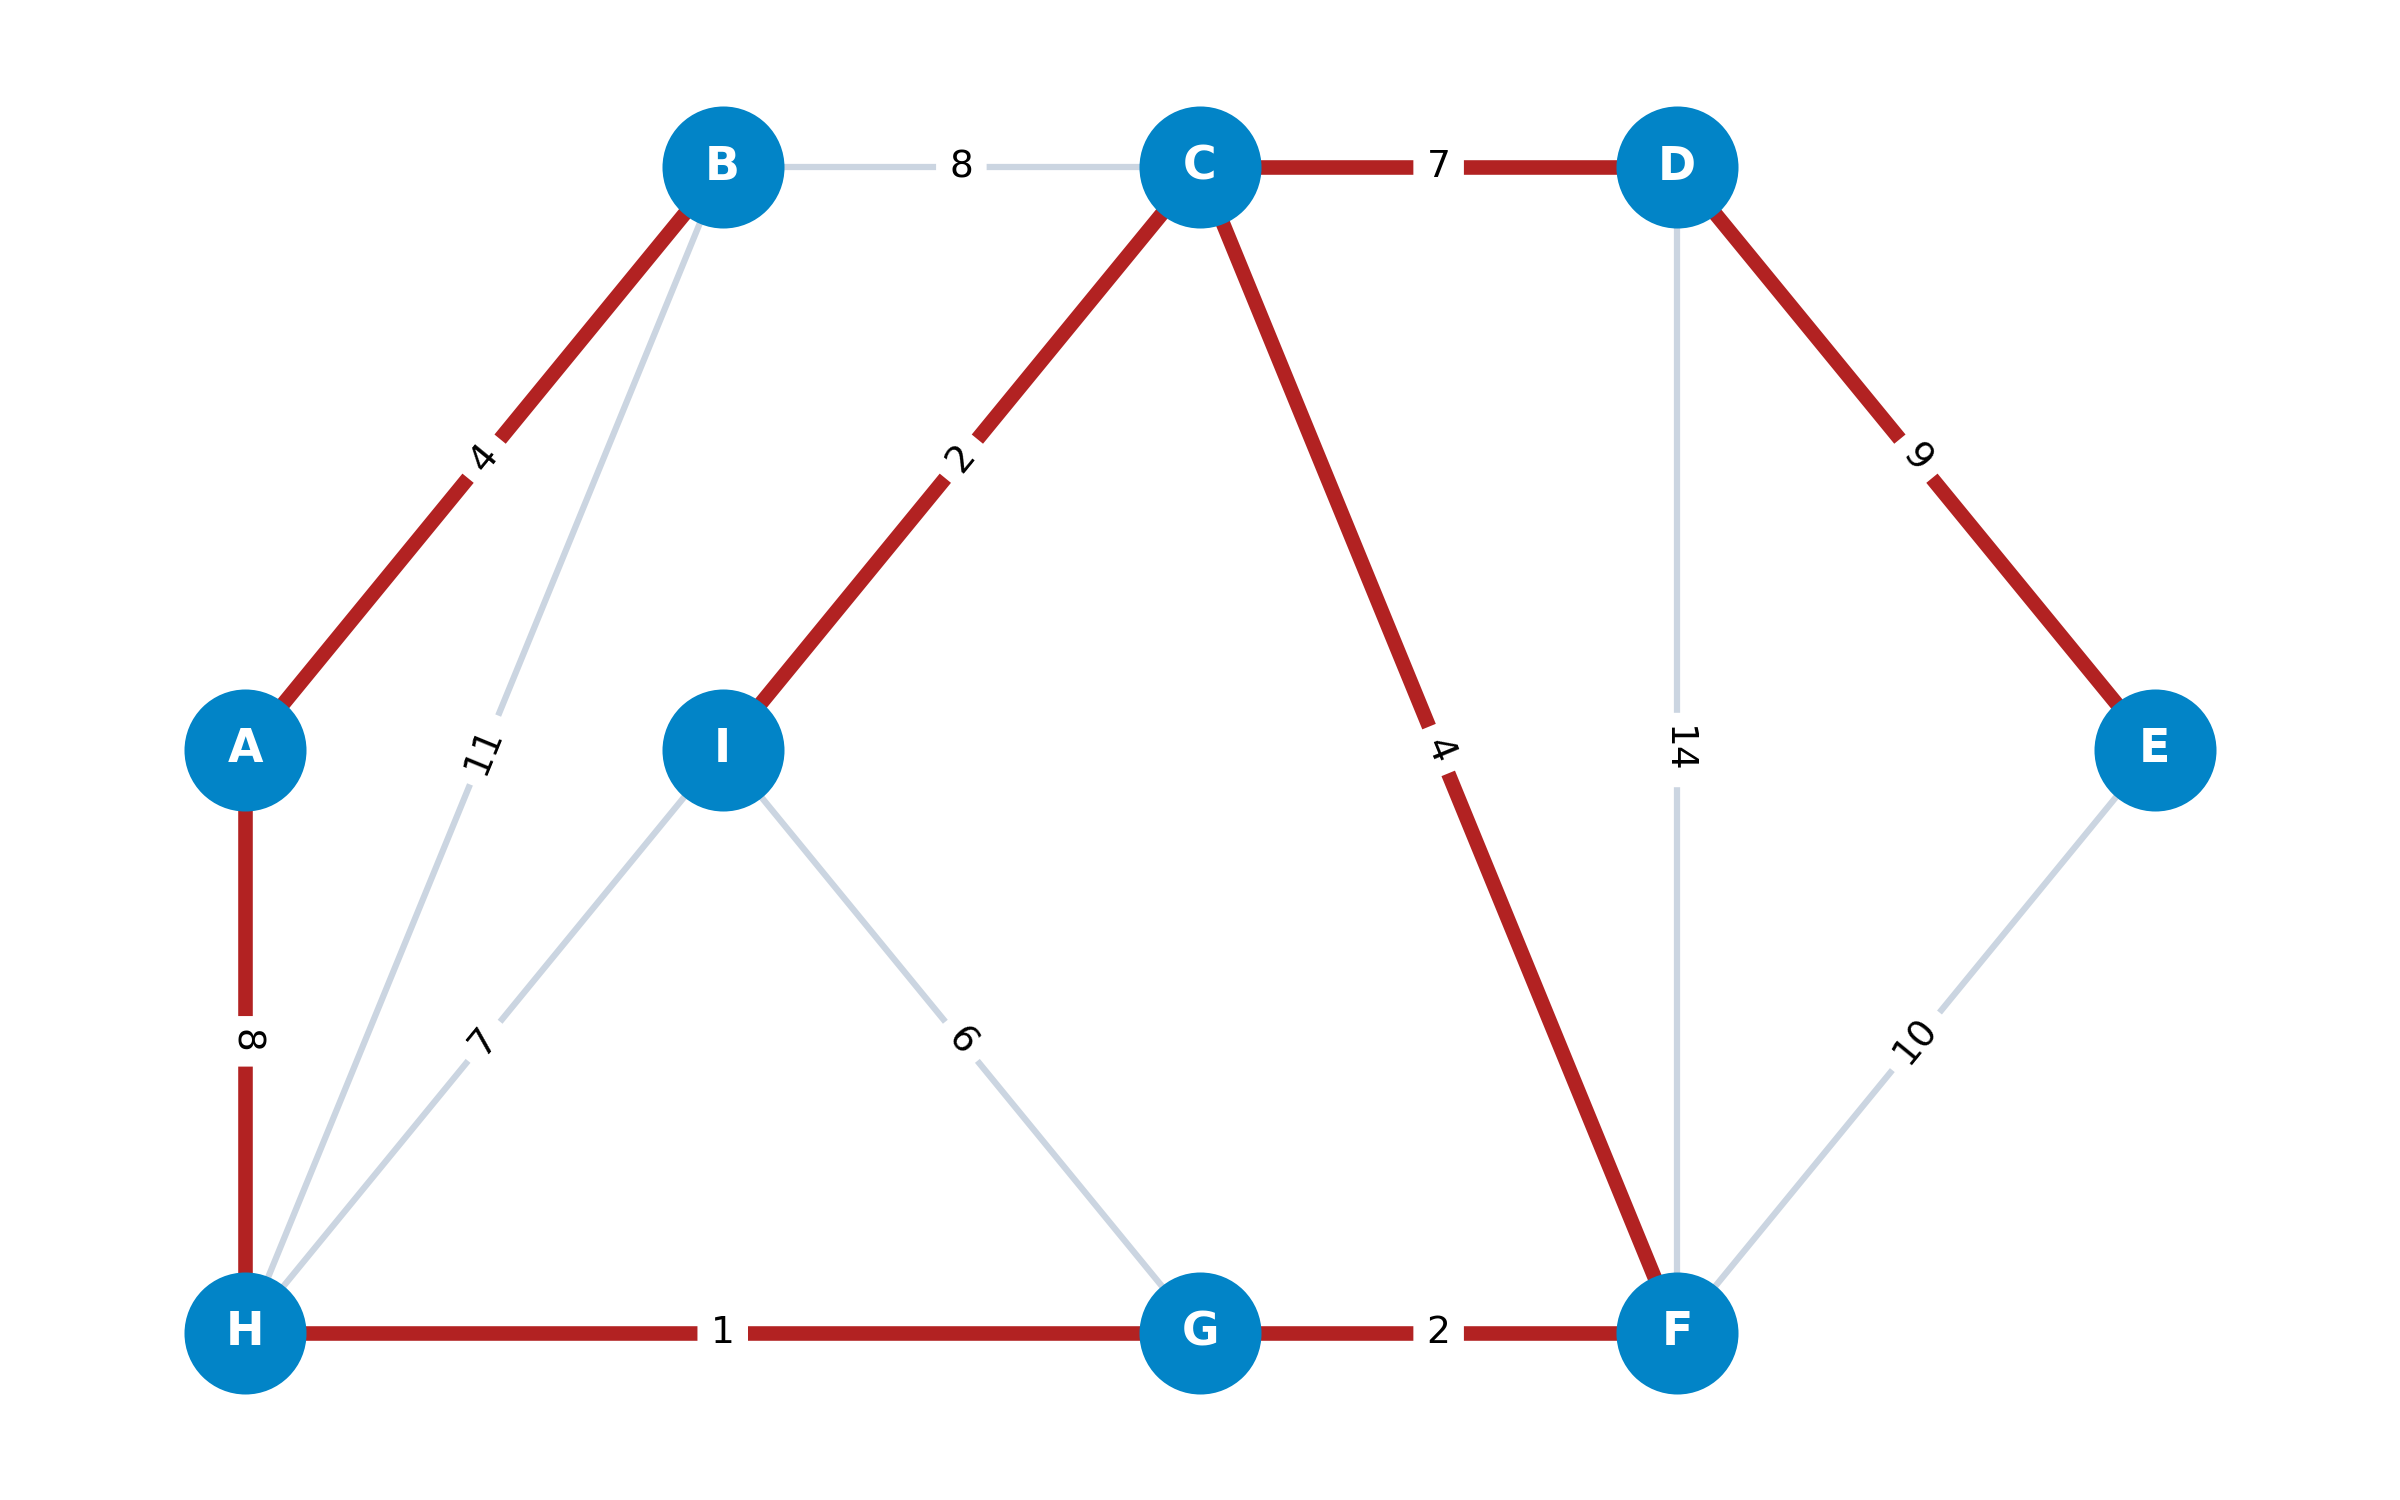
\includegraphics[width=0.75\linewidth,height=\textheight,keepaspectratio]{images/prim_traza_paso_a_paso.png}

}

\caption{\label{fig-prim-ejemplo-pasos}Traza gráfica de la evolución
iterativa del Algoritmo de Prim paso a paso}

\end{figure}%

\textbf{Conclusión y Peso del Árbol Soporte de Mínimo Peso}: Al
cumplirse \(P = V\) (o de forma equivalente \(|T| = n - 1 = 5\)), el
proceso finaliza. El árbol soporte de mínimo peso \(H = (V, T)\) acumula
un peso total idéntico al obtenido por Kruskal: \[
d(T) = d_{\{1,2\}} + d_{\{2,5\}} + d_{\{2,4\}} + d_{\{4,6\}} + d_{\{1,3\}} = 1 + 3 + 4 + 3 + 5 = 16
\]

\textbf{Observación sobre la Solución Alternativa}: Puesto que en la
iteración \(i=5\) existía un empate de peso mínimo (\(d=5\)) entre las
aristas del corte \(\{1, 3\}\) y \(\{3, 4\}\), si en lugar de
seleccionar \(\{1, 3\}\) se hubiera optado por incorporar \(\{3, 4\}\),
se obtendría una \textbf{solución alternativa}: \[
T' = \{\{1, 2\}, \{2, 5\}, \{2, 4\}, \{4, 6\}, \{3, 4\}\}
\] El peso acumulado en esta arborescencia alternativa es
\(d(T') = 1 + 3 + 4 + 3 + 5 = 16\), exactamente igual al peso del árbol
\(T\). Esto reafirma de forma consistente que el Algoritmo de Prim y el
Algoritmo de Kruskal llegan al mismo valor del peso del Árbol Soporte de
Mínimo Peso (\(d(T) = 16\)), produciendo la misma familia de soluciones
óptimas alternativas ante empates en los pesos de las aristas.

\end{tcolorbox}

\begin{center}\rule{0.5\linewidth}{0.5pt}\end{center}

\subsection{Aplicaciones en aprendizaje no supervisado: clustering
basado en
MST}\label{aplicaciones-en-aprendizaje-no-supervisado-clustering-basado-en-mst}

En la ciencia de datos moderna y el aprendizaje automático
(\emph{machine learning}), uno de los objetivos esenciales del
aprendizaje no supervisado (trabajo con datos no etiquetados) es
descubrir patrones latentes y estructurar el conjunto de observaciones
en grupos o clústeres homogéneos (\textbf{clustering}).

La agrupación de datos se realiza en función de la semejanza o
desemejanza entre las observaciones.

\begin{tcolorbox}[enhanced jigsaw, toprule=.15mm, opacitybacktitle=0.6, coltitle=black, colbacktitle=quarto-callout-note-color!10!white, title=\textcolor{quarto-callout-note-color}{\faInfo}\hspace{0.5em}{Definición: Medida de desemejanza y distancia}, arc=.35mm, rightrule=.15mm, toptitle=1mm, breakable, bottomtitle=1mm, titlerule=0mm, colback=white, opacityback=0, leftrule=.75mm, colframe=quarto-callout-note-color-frame, left=2mm, bottomrule=.15mm]

Dada una colección de observaciones o variables \(x, y\), una
\textbf{función de desemejanza} \(\delta(x, y)\) asigna un valor
numérico real que cuantifica la divergencia entre ambas observaciones,
satisfaciendo las siguientes propiedades fundamentales:

\begin{enumerate}
\def\labelenumi{\arabic{enumi}.}
\tightlist
\item
  \textbf{Coincidencia nula}: \(\delta(x, y) = 0 \iff x = y\).
\item
  \textbf{No negatividad}: \(\delta(x, y) \ge 0\) para todo \(x, y\).
\item
  \textbf{Simetría}: \(\delta(x, y) = \delta(y, x)\).
\end{enumerate}

Si además la función verifica la \textbf{desigualdad triangular}
\(\delta(x, y) \le \delta(x, z) + \delta(y, z)\), la medida constituye
una \textbf{distancia métrica} en sentido estricto (como la distancia
euclídea \(\|x - y\|_2\)).

\end{tcolorbox}

\begin{tcolorbox}[enhanced jigsaw, toprule=.15mm, opacitybacktitle=0.6, coltitle=black, colbacktitle=quarto-callout-note-color!10!white, title=\textcolor{quarto-callout-note-color}{\faInfo}\hspace{0.5em}{Comparativa: k-Medias frente a clustering basado en MST}, arc=.35mm, rightrule=.15mm, toptitle=1mm, breakable, bottomtitle=1mm, titlerule=0mm, colback=white, opacityback=0, leftrule=.75mm, colframe=quarto-callout-note-color-frame, left=2mm, bottomrule=.15mm]

\begin{itemize}
\item
  \textbf{Algoritmo de las \(k\)-Medias (\emph{\(k\)-means})}:

  Es la técnica no supervisada más popular para particionar un conjunto
  de datos en \(K\) clústeres disjuntos \(S = \{S_1, \dots, S_K\}\)
  tales que \(S_i \cap S_j = \emptyset\) para todo \(i \neq j\),
  minimizando la variabilidad dentro de cada grupo (\emph{within-cluster
  variation}): \[
  W(S, c) = \sum_{k=1}^K W(S_k) = \sum_{k=1}^K \sum_{x_i \in S_k} \|x_i - c_k\|^2
  \] donde \(c_k\) representa el centroide (media aritmética) del
  clúster \(S_k\). Al estar basado en regiones de Voronoi delimitadas
  por hiperplanos, exige implícitamente que los clústeres posean una
  geometría esférica o convexa.
\item
  \textbf{Clustering basado en el Árbol Soporte de Mínimo Peso (MST)}:
  Modela el conjunto de \(n\) observaciones como una red completa
  \(G = (V, E, \delta)\) y calcula su MST \(T = (V, E')\). Al eliminar
  las \(K - 1\) aristas de mayor peso (mayor desemejanza), particiona la
  red de forma determinista en \(K\) componentes conexas de geometría
  arbitraria y no lineal.
\end{itemize}

\end{tcolorbox}

Como se ilustra en la Figura~\ref{fig-mst-clustering-ejemplo}, en el
panel izquierdo se construye el Árbol Soporte de Mínimo Peso completo
sobre \(n = 9\) observaciones valoradas por su desemejanza. Al
identificar y cortar las \(K - 1 = 2\) aristas de mayor peso (la arista
\(\{2, 4\}\) de longitud \(8.5\) y \(\{3, 7\}\) de longitud \(7.0\),
resaltadas en línea discontinua), el grafo se particiona de forma
determinista en \(K = 3\) clústeres disjuntos bien delimitados (panel
derecho).

\begin{figure}

\centering{

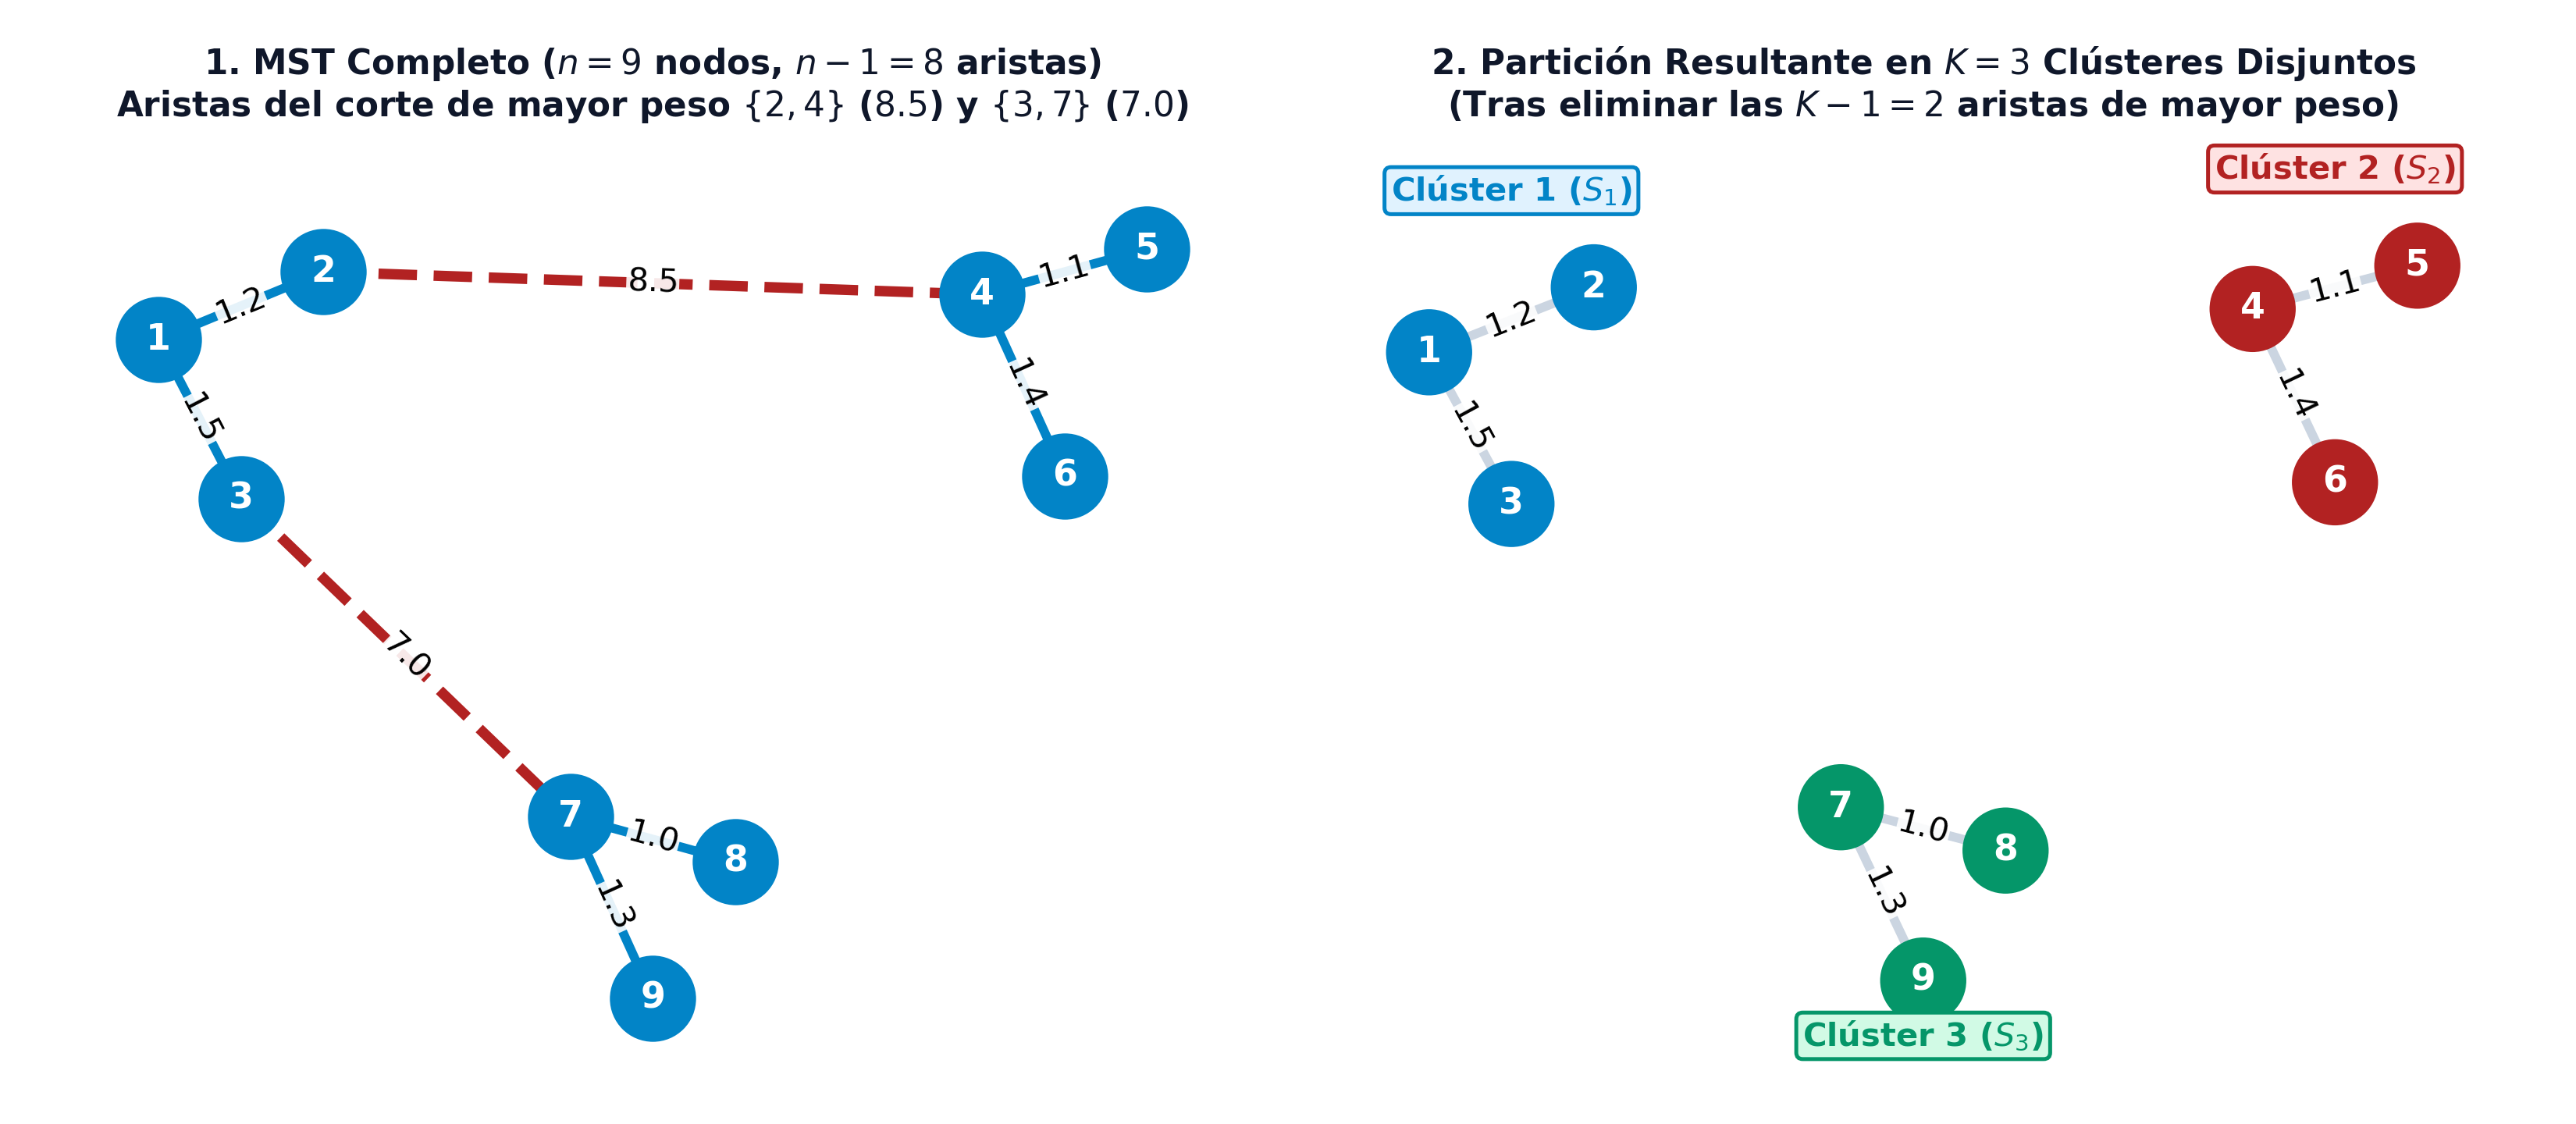
\includegraphics[width=0.95\linewidth,height=\textheight,keepaspectratio]{images/mst_clustering_ejemplo.png}

}

\caption{\label{fig-mst-clustering-ejemplo}Proceso de agrupamiento
(\emph{clustering}) mediante el MST: identificación y corte de las
\(K-1=2\) aristas de mayor peso (panel izquierdo) y partición resultante
en \(K=3\) clústeres disjuntos (panel derecho)}

\end{figure}%

En la Figura~\ref{fig-mst-clustering-complejo} se observa la capacidad
superior del agrupamiento basado en MST para resolver conjuntos de datos
con geometrías no convexas complejas (como anillos concéntricos o lunas
entrelazadas), situaciones en las que el algoritmo de \(k\)-medias
fracasa al imponer fronteras rígidas de Voronoi.

\begin{figure}

\centering{

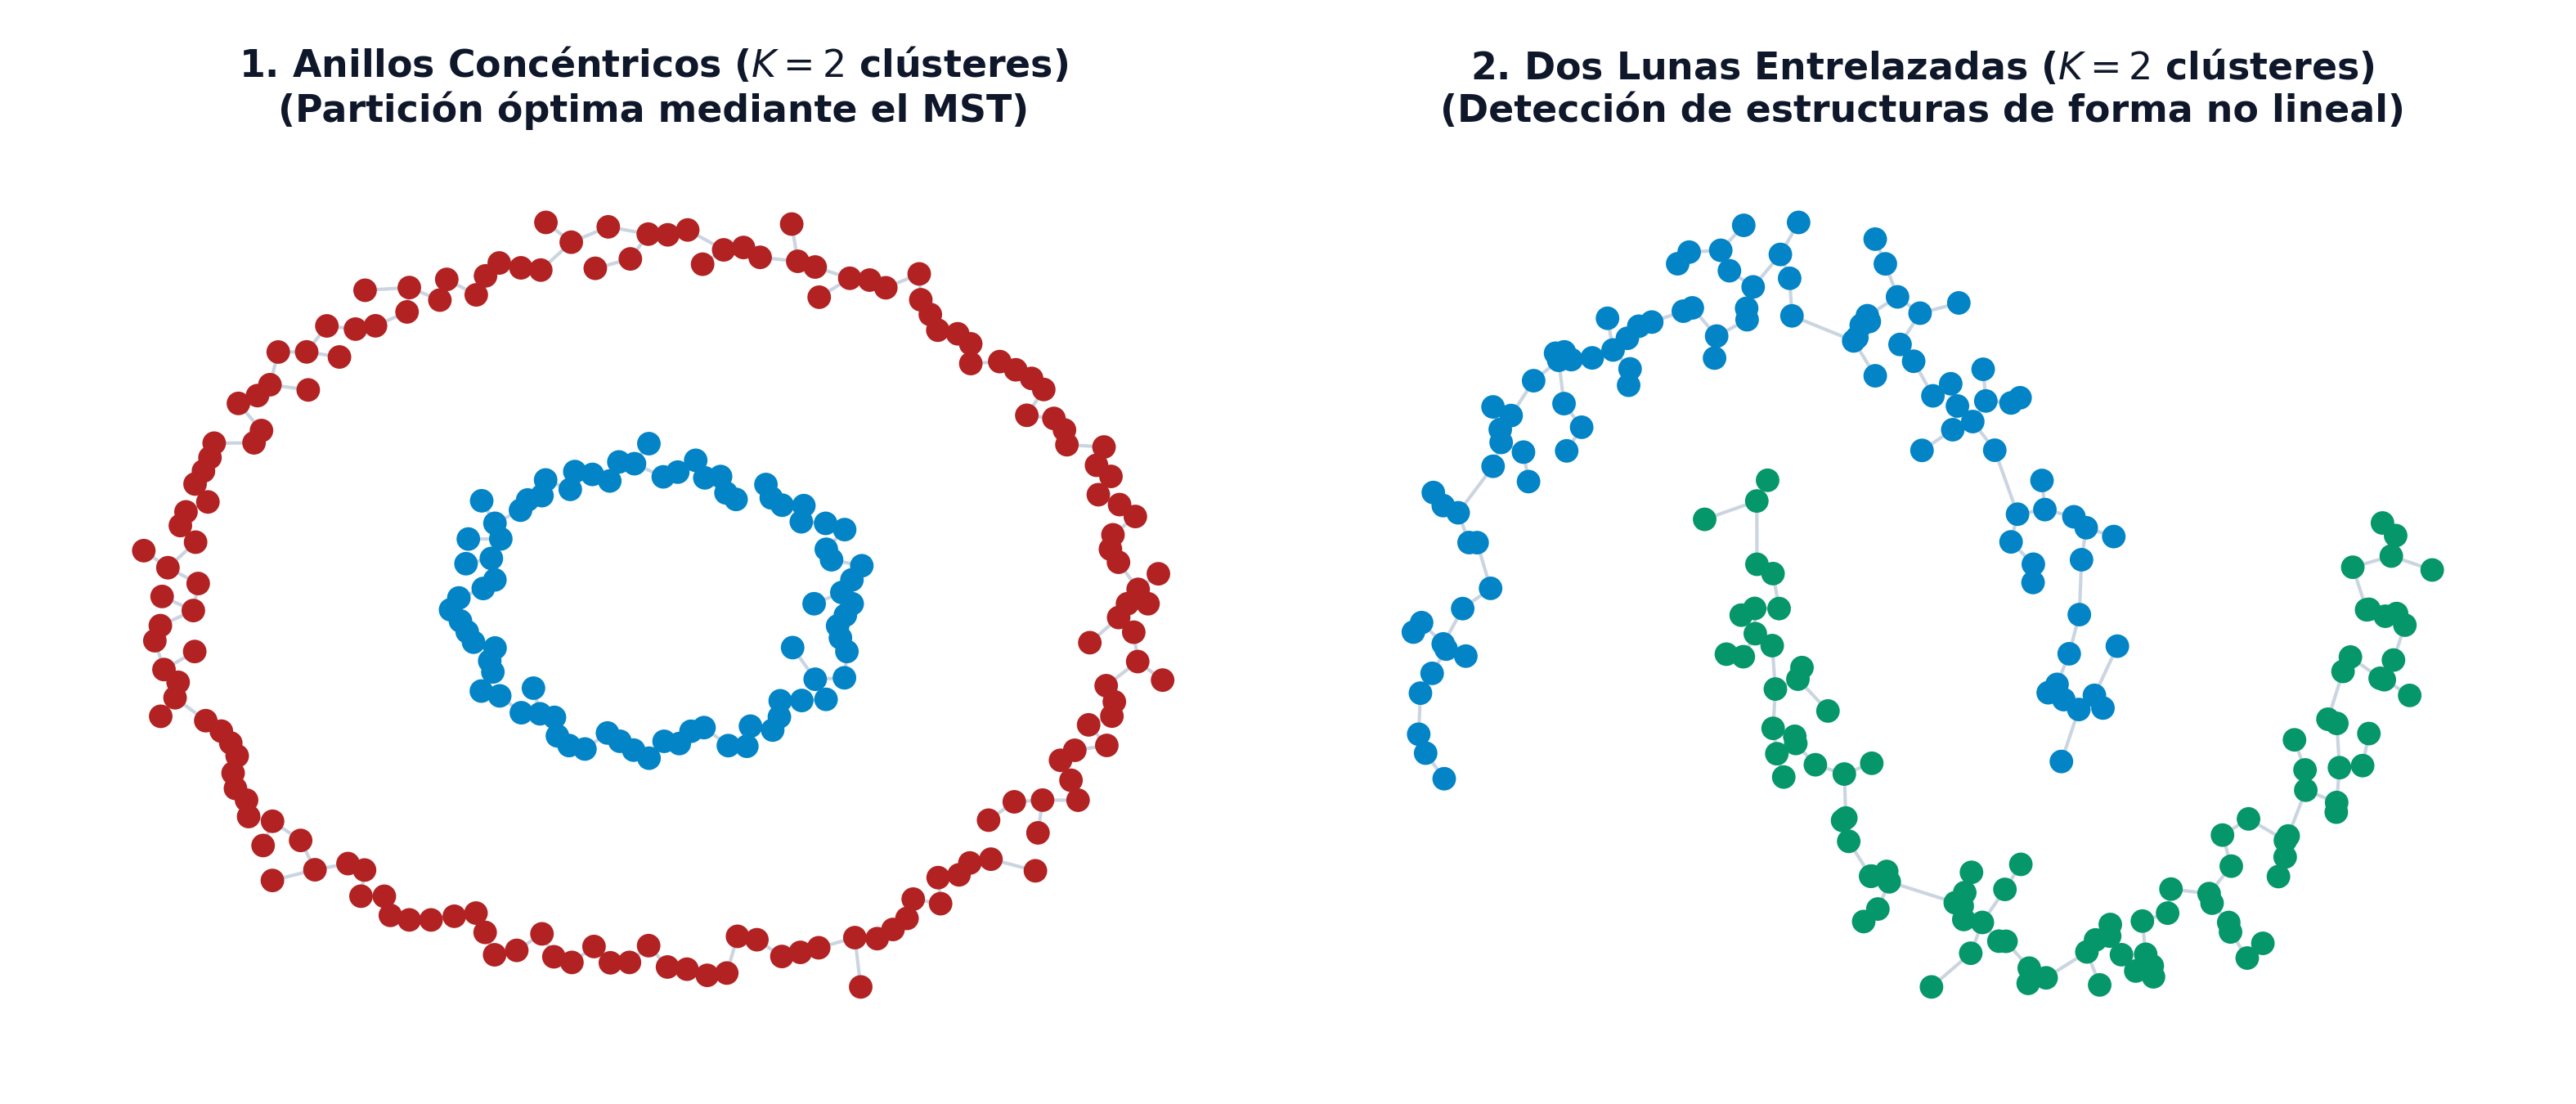
\includegraphics[width=0.95\linewidth,height=\textheight,keepaspectratio]{images/mst_clustering_complejo.png}

}

\caption{\label{fig-mst-clustering-complejo}Detección de estructuras de
forma no lineal mediante el MST: agrupamiento en anillos concéntricos
(panel izquierdo) y dos lunas entrelazadas (panel derecho)}

\end{figure}%

\textbf{Generalización mediante Funciones de Calidad de la Partición}:
Aunque la regla primaria consiste en quitar los \(K - 1\) enlaces de
mayor peso del MST, es posible encontrar criterios de decisión mucho más
elaborados y adaptados a la estructura de los datos mediante una función
de evaluación objetiva.

Sea \(\mathcal{X}_\ell\) el conjunto de posibles particiones del
conjunto de observaciones \(\mathbf{X}\) en \(\ell\) clústeres o
componentes conexas disjuntas. Dado un subgrafo \(G' = (V, E'')\) con
\(\ell\) componentes conexas, denotamos por
\(C(V, E'') = (X_1, X_2, \dots, X_\ell) \in \mathcal{X}_\ell\) a la
partición asociada a \(G'\). Se define una función de calidad o validez
\(F : \mathcal{X}_\ell \to \mathbb{R}\) que evalúa la bondad de la
partición. El objetivo consiste en encontrar la partición que maximiza
la función \(F\).

Para maximizar \(F\) sobre el MST se aplica un procedimiento voraz
(\emph{greedy}) divisivo:

\begin{tcolorbox}[enhanced jigsaw, toprule=.15mm, opacitybacktitle=0.6, coltitle=black, colbacktitle=quarto-callout-note-color!10!white, title=\textcolor{quarto-callout-note-color}{\faInfo}\hspace{0.5em}{Esquema: Maximización de la función de calidad F sobre el MST}, arc=.35mm, rightrule=.15mm, toptitle=1mm, breakable, bottomtitle=1mm, titlerule=0mm, colback=white, opacityback=0, leftrule=.75mm, colframe=quarto-callout-note-color-frame, left=2mm, bottomrule=.15mm]

Dada una red de datos \(G = (V, E, \delta)\) y una función de calidad
\(F\):

\begin{enumerate}
\def\labelenumi{\arabic{enumi}.}
\tightlist
\item
  \textbf{Paso 1}: Obtener el árbol soporte de mínimo peso
  \(T = \text{MST}(G) = (V, E', \delta)\).
\item
  \textbf{Paso 2}: Inicializar el conjunto de aristas activas
  \(E'' = E'\).
\item
  \textbf{Paso 3}: Para \(i = 1, \dots, K - 1\), hacer:

  \begin{itemize}
  \tightlist
  \item
    Identificar la arista \(\{u, v\} \in E''\) cuya eliminación maximice
    la calidad de la partición resultante: \[
    \{u, v\} = \arg\max_{e \in E''} F(C(V, E'' \setminus \{e\}))
    \]
  \item
    Eliminar la arista \(\{u, v\}\) de \(E''\):
    \(E'' \leftarrow E'' \setminus \{\{u, v\}\}\).
  \end{itemize}
\item
  \textbf{Paso 4}: Terminar y devolver la partición \(C(V, E'')\) como
  resultado.
\end{enumerate}

\end{tcolorbox}

\begin{tcolorbox}[enhanced jigsaw, toprule=.15mm, opacitybacktitle=0.6, coltitle=black, colbacktitle=quarto-callout-note-color!10!white, title=\textcolor{quarto-callout-note-color}{\faInfo}\hspace{0.5em}{Criterios y funciones de calidad F en la literatura}, arc=.35mm, rightrule=.15mm, toptitle=1mm, breakable, bottomtitle=1mm, titlerule=0mm, colback=white, opacityback=0, leftrule=.75mm, colframe=quarto-callout-note-color-frame, left=2mm, bottomrule=.15mm]

En la literatura científica se emplean diversas especificaciones para la
función de calidad \(F\):

\begin{itemize}
\item
  \textbf{Criterio de mayor longitud (Separación)}: \[
  F(X_1, \dots, X_\ell) = \sum_{i=1}^\ell \sum_{x_j \in X_i} x_j
  \] (Equivalente a eliminar de forma directa las \(K - 1\) aristas de
  mayor peso en el MST).
\item
  \textbf{Suma de cuadrados intra-grupo negativa (\(-WCSS\))}: \[
  -WCSS(X_1, \dots, X_\ell) = -\sum_{i=1}^\ell \sum_{x_j \in X_i} \|x_j - \mu_i\|^2
  \] donde \(\mu_i\) representa el centroide del \(i\)-ésimo clúster.
\item
  \textbf{Criterio de información / entropía (\(IC\))}: \[
  IC(X_1, \dots, X_\ell) = -d \sum_{i=1}^\ell \frac{n_i}{n} \log \frac{L_i}{n_i} - \sum_{i=1}^\ell \frac{n_i}{n} \log \frac{n_i}{n}
  \] donde \(L_i\) es la suma de los pesos de las aristas en el subárbol
  asociado al \(i\)-ésimo clúster y \(n_i\) es el número de
  observaciones en ese grupo.
\item
  \textbf{Desviación típica de los pesos de las aristas}: Minimización
  de la dispersión de las distancias entre aristas dentro de los
  clústeres.
\end{itemize}

\end{tcolorbox}

\begin{tcolorbox}[enhanced jigsaw, toprule=.15mm, opacitybacktitle=0.6, coltitle=black, colbacktitle=quarto-callout-warning-color!10!white, title=\textcolor{quarto-callout-warning-color}{\faExclamationTriangle}\hspace{0.5em}{Estrategia aglomerativa e inconvenientes prácticos}, arc=.35mm, rightrule=.15mm, toptitle=1mm, breakable, bottomtitle=1mm, titlerule=0mm, colback=white, opacityback=0, leftrule=.75mm, colframe=quarto-callout-warning-color-frame, left=2mm, bottomrule=.15mm]

Una alternativa al algoritmo divisivo anterior consiste en utilizar una
estrategia aglomerativa o acumulativa (de filosofía análoga al Algoritmo
de Kruskal): comenzar con \(E'' = \emptyset\) e ir añadiendo aristas una
a una del MST que maximicen la función \(F(C(V, E'' \cup \{\{u,v\}\}))\)
hasta alcanzar \(K\) componentes conexas.

Sin embargo, esta aproximación aglomerativa resulta computacionalmente
menos eficiente y puede presentar problemas cuando se forman grupos
aislados con muy pocas observaciones en las iteraciones iniciales. Para
resolver esta inestabilidad, diversos autores modifican el algoritmo
introduciendo penalizaciones o restricciones (utilizando el
\textbf{índice de Gini}) que dan prioridad a los grupos más pequeños
cuando existe una disparidad excesiva en la dimensión de los clústeres.

\end{tcolorbox}

\chapter{Caminos mínimos}\label{caminos-muxednimos}

El \textbf{problema del camino mínimo} (\emph{Shortest Path Problem})
constituye una de las piedras angulares de la optimización de redes y de
la investigación operativa contemporánea (Ahuja, Magnanti, y Orlin 1993;
Bertsekas 1998; Cormen et~al. 2009). Su propósito fundamental es
determinar la ruta de menor coste, distancia o tiempo acumulado entre un
nodo origen \(s\) y un nodo destino \(t\), o bien desde un origen único
hacia la totalidad de los vértices de una red.

Más allá de sus aplicaciones inmediatas en la planificación de
transporte, la navegación GPS, el enrutamiento de paquetes en redes de
telecomunicaciones y la logística de distribución, el problema del
camino mínimo actúa como subproblema crítico en algoritmos de mayor
envergadura, tales como los métodos de generación de columnas en
programación entera, el diseño de redes de flujo de coste mínimo y la
programación dinámica multietapa.

\begin{tcolorbox}[enhanced jigsaw, toprule=.15mm, opacitybacktitle=0.6, coltitle=black, colbacktitle=quarto-callout-important-color!10!white, title=\textcolor{quarto-callout-important-color}{\faExclamation}\hspace{0.5em}{Objetivos de aprendizaje}, arc=.35mm, rightrule=.15mm, toptitle=1mm, breakable, bottomtitle=1mm, titlerule=0mm, colback=white, opacityback=0, leftrule=.75mm, colframe=quarto-callout-important-color-frame, left=2mm, bottomrule=.15mm]

Al finalizar este capítulo, serás capaz de:

\begin{enumerate}
\def\labelenumi{\arabic{enumi}.}
\tightlist
\item
  \textbf{Formular y fundamentar} el problema del camino mínimo en
  digrafos valorados definiendo formalmente su matriz de distancias
  directas y analizando las condiciones de existencia de solución óptima
  finita.
\item
  \textbf{Deducir y resolver} las ecuaciones de optimalidad de Bellman a
  partir del Principio de Optimalidad de la programación dinámica,
  identificando las causas de insuficiencia ante circuitos de coste nulo
  o negativo.
\item
  \textbf{Aplicar la ordenación topológica} en redes acíclicas (DAGs)
  para calcular caminos mínimos en tiempo lineal \(O(|V| + |A|)\).
\item
  \textbf{Demostrar y ejecutar} el algoritmo de Dijkstra en redes con
  costes no negativos, comprendiendo su carácter goloso y su complejidad
  computacional.
\item
  \textbf{Programar y evaluar} el algoritmo de Bellman-Ford para redes
  con arcos de coste negativo, aplicando el criterio de detección de
  circuitos de coste negativo en tiempo \(O(|V| \cdot |A|)\).
\item
  \textbf{Formular y analizar} el problema mediante programación lineal
  primal-dual, justificando la integridad de las soluciones mediante la
  Total Unimodularidad (TUM) de la matriz de incidencia nodo-arco e
  interpretando los potenciales nodales duales.
\item
  \textbf{Calcular distancias entre todos los pares de nodos} aplicando
  el algoritmo de multiplicación de matrices en álgebra min-suma y la
  relación de recurrencia de programación dinámica del algoritmo de
  Floyd-Warshall.
\end{enumerate}

\end{tcolorbox}

\begin{center}\rule{0.5\linewidth}{0.5pt}\end{center}

\section{Definición formal y condiciones de
existencia}\label{definiciuxf3n-formal-y-condiciones-de-existencia}

Consideremos un digrafo conexo valorado \(G = (V, U, \mathbf{d})\),
donde \(V = \{1, 2, \dots, n\}\) representa el conjunto de vértices o
nodos, \(U \subseteq V \times V\) denota el conjunto de arcos dirigidos
con cardinalidad \(|U| = m\), y \(\mathbf{d} \in \mathbb{R}^m\) es un
vector cuyas componentes \(d(u) = d_{ij}\) asignan un coste, tiempo o
distancia a cada arco dirigido \(u = (i, j) \in U\).

\begin{tcolorbox}[enhanced jigsaw, toprule=.15mm, opacitybacktitle=0.6, coltitle=black, colbacktitle=quarto-callout-note-color!10!white, title=\textcolor{quarto-callout-note-color}{\faInfo}\hspace{0.5em}{Definición: Red valorada y longitud de un camino}, arc=.35mm, rightrule=.15mm, toptitle=1mm, breakable, bottomtitle=1mm, titlerule=0mm, colback=white, opacityback=0, leftrule=.75mm, colframe=quarto-callout-note-color-frame, left=2mm, bottomrule=.15mm]

Dado un camino dirigido \(\mu = (v_0, v_1, v_2, \dots, v_k)\) en \(G\),
compuesto por una secuencia de arcos \((v_{j-1}, v_j) \in U\) para todo
\(j = 1, \dots, k\), la \textbf{longitud o coste acumulado del camino}
\(d(\mu)\) se define como la suma de las longitudes de los arcos que lo
integran:

\[
d(\mu) = \sum_{u \in \mu} d_u = \sum_{j=1}^k d_{v_{j-1}, v_j}
\]

\end{tcolorbox}

Para formalizar algebraicamente las conexiones de la red, se introduce
la \textbf{matriz de distancias directas}
\(D \in \overline{\mathbb{R}}^{n \times n}\), cuyas componentes
\(d_{ij}\) se definen para todo par de vértices \(i, j \in V\) como:

\[
d_{ij} = \begin{cases} 
0 & \text{si } i = j \\ 
d_u & \text{si } u = (i, j) \in U \\ 
+\infty & \text{si } (i, j) \notin U \text{ y } i \neq j 
\end{cases}
\]

Esta representación matricial permite modelar problemas de transporte,
telecomunicaciones y logística de variada naturaleza, como se ilustra en
los dos ejemplos siguientes.

\begin{tcolorbox}[enhanced jigsaw, toprule=.15mm, opacitybacktitle=0.6, coltitle=black, colbacktitle=quarto-callout-tip-color!10!white, title=\textcolor{quarto-callout-tip-color}{\faLightbulb}\hspace{0.5em}{Ejemplo: Red de itinerarios de vuelos internacionales}, arc=.35mm, rightrule=.15mm, toptitle=1mm, breakable, bottomtitle=1mm, titlerule=0mm, colback=white, opacityback=0, leftrule=.75mm, colframe=quarto-callout-tip-color-frame, left=2mm, bottomrule=.15mm]

Un viajero desea planificar la ruta de coste mínimo para volar desde
Madrid (\(M\)) hasta Tokio (\(T\)). Al no existir un vuelo directo, debe
realizar al menos una escala en los aeropuertos intermedios de Londres
(\(L\)), París (\(P\)), Frankfurt (\(F\)) o Singapur (\(S\)).

El problema se modela sobre un digrafo \(G = (V, U)\) donde los vértices
representan los aeropuertos \(V = \{M, L, F, P, S, T\}\) y los arcos
corresponden a los vuelos directos disponibles con sus respectivas
tarifas en euros:

\begin{itemize}
\tightlist
\item
  Desde \(M\): arcos \((M, L)\) con coste 20, \((M, F)\) con coste 40,
  \((M, P)\) con coste 27.
\item
  Desde \(L\): arco \((L, F)\) con coste 10.
\item
  Entre \(F\) y \(P\): arcos bidireccionales \((F, P)\) con coste 11 y
  \((P, F)\) con coste 9.
\item
  Desde \(F\) y \(P\) hacia Asia: \((F, S)\) con coste 90, \((P, S)\)
  con coste 100, \((P, T)\) con coste 150.
\item
  Desde \(S\): arco \((S, T)\) con coste 35.
\end{itemize}

Como se ilustra en la Figura~\ref{fig-cminimo-ejemplo-vuelos}, la
resolución de este problema consiste en hallar la secuencia de arcos
dirigidos que conecte \(M\) con \(T\) minimizando el sumatorio de las
tarifas asociadas.

\begin{figure}[H]

\centering{

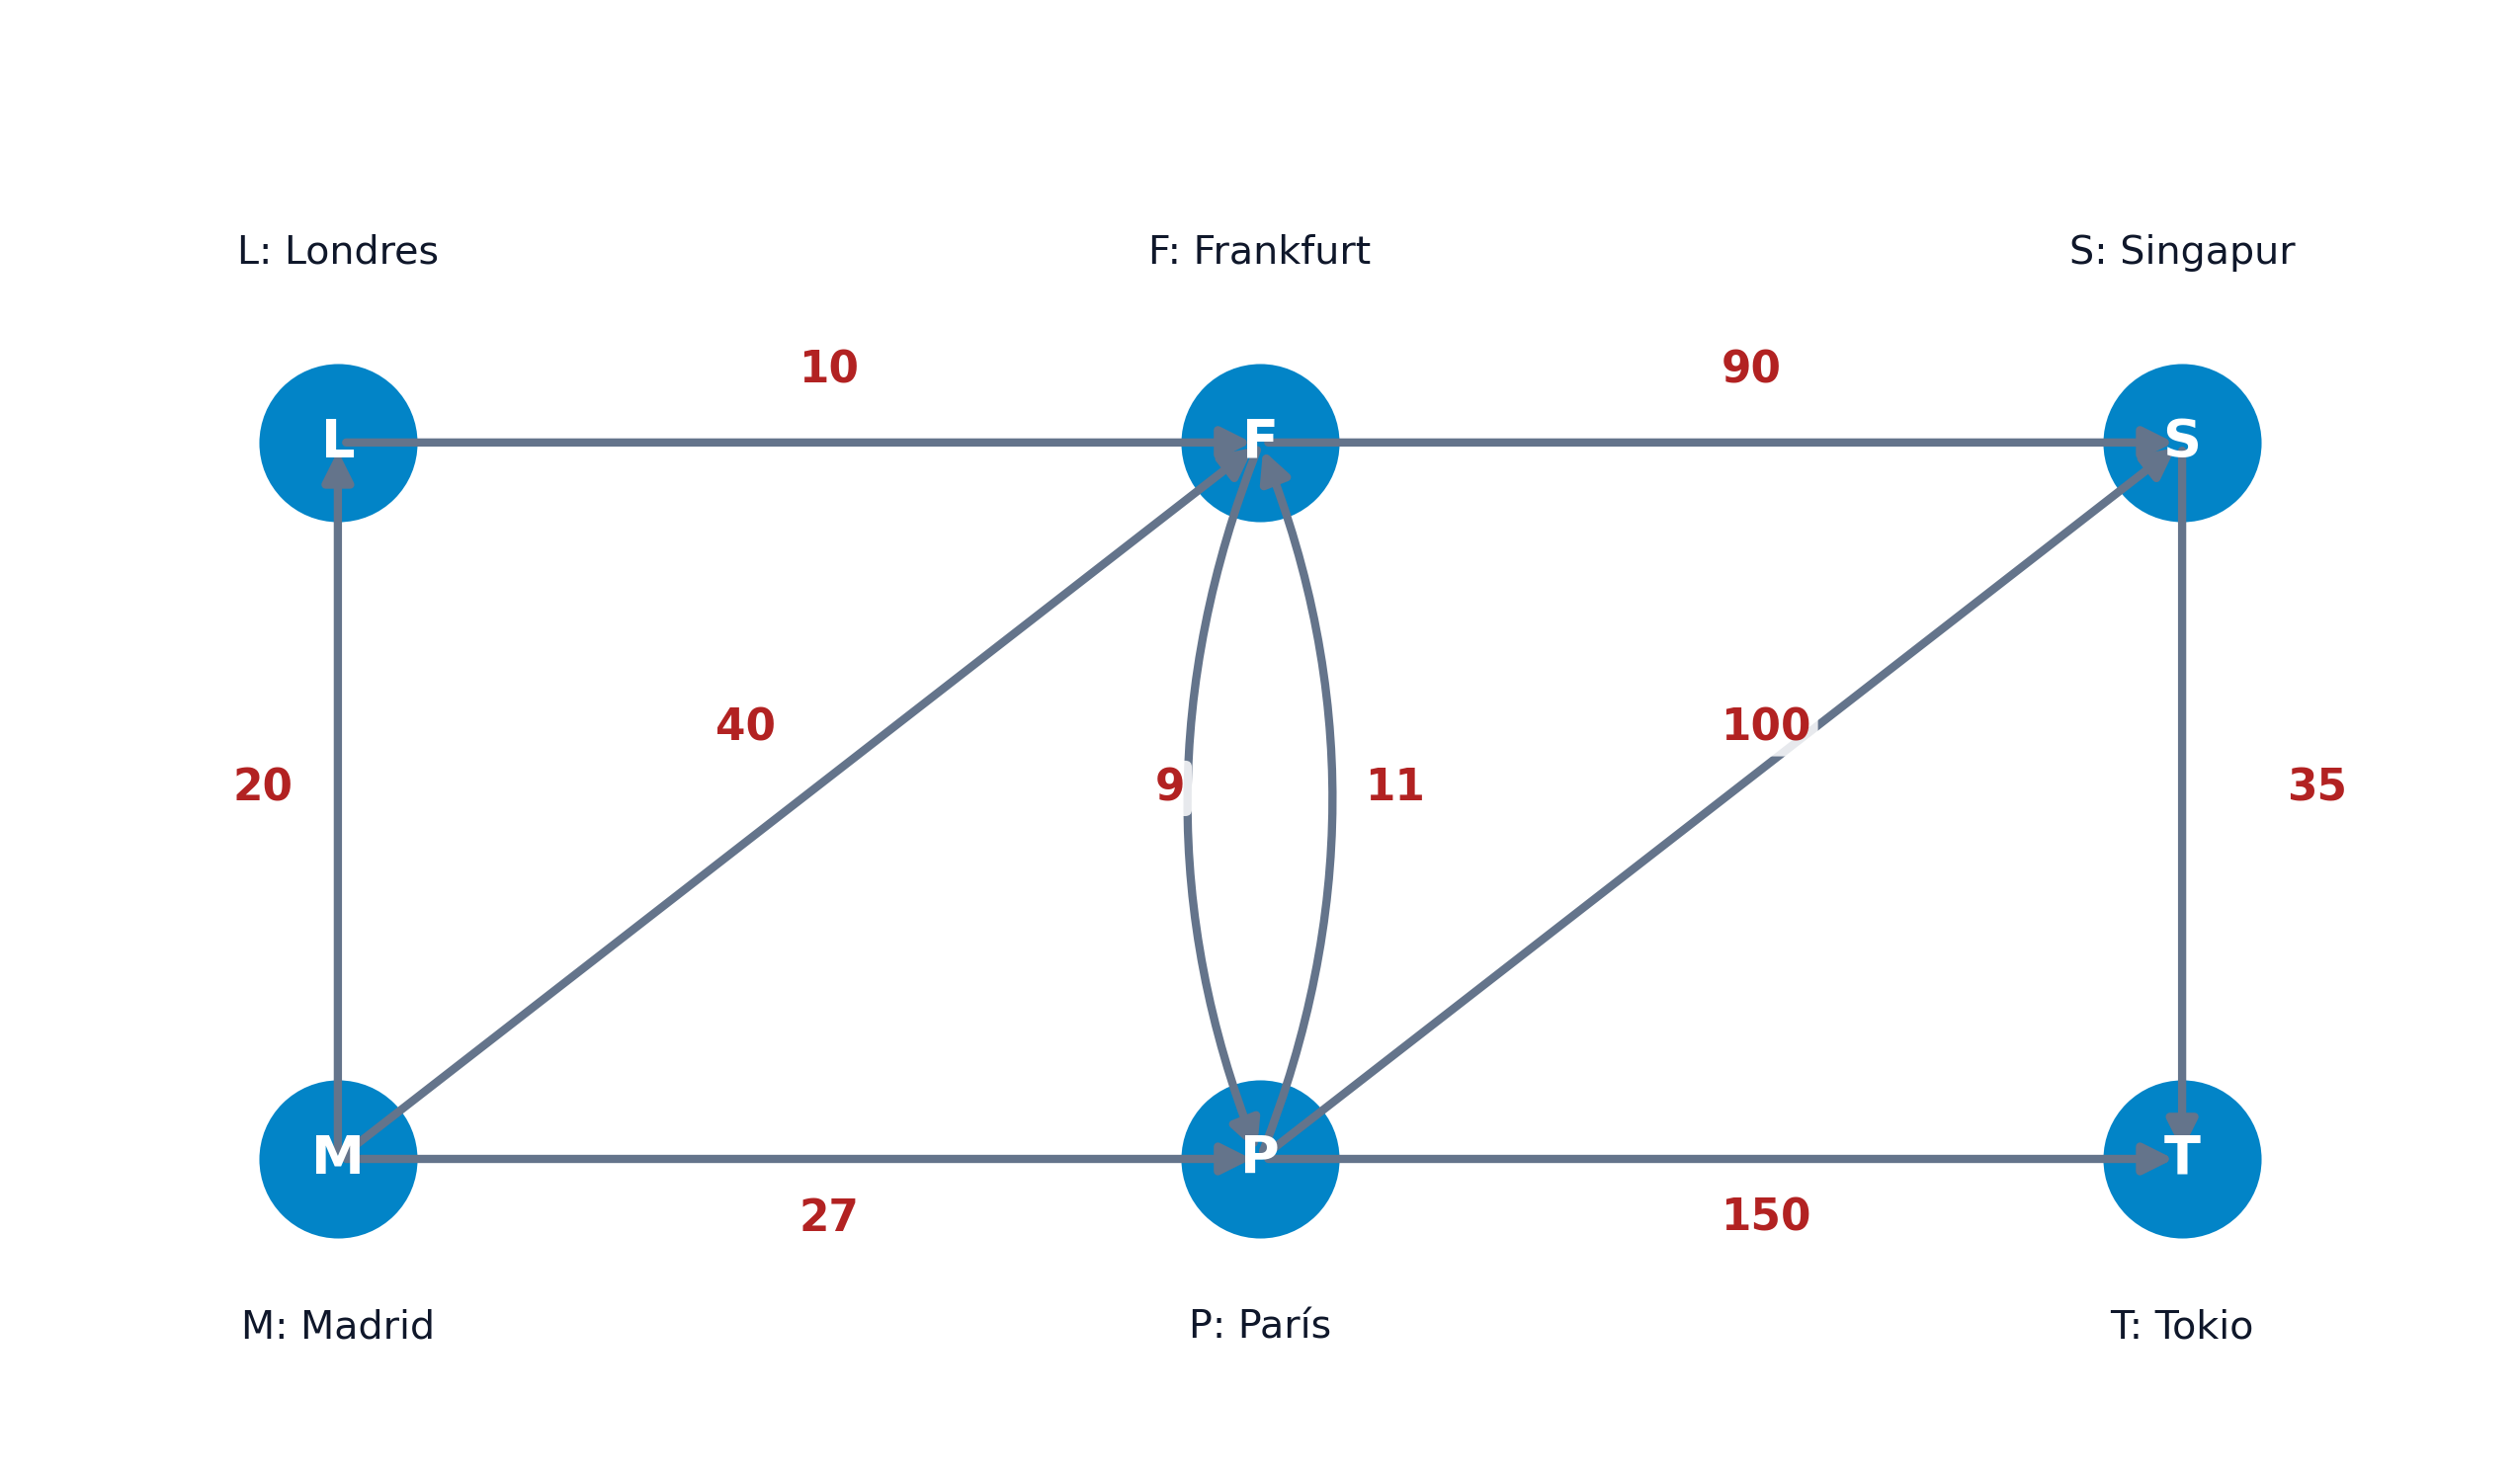
\includegraphics[width=0.75\linewidth,height=\textheight,keepaspectratio]{images/cminimo_ejemplo_vuelos.png}

}

\caption{\label{fig-cminimo-ejemplo-vuelos}Representación en digrafo
valorado del problema de itinerarios de vuelos internacionales entre
Madrid y Tokio}

\end{figure}%

\end{tcolorbox}

\begin{tcolorbox}[enhanced jigsaw, toprule=.15mm, opacitybacktitle=0.6, coltitle=black, colbacktitle=quarto-callout-tip-color!10!white, title=\textcolor{quarto-callout-tip-color}{\faLightbulb}\hspace{0.5em}{Ejemplo: Planificación de transporte marítimo con costes y beneficios}, arc=.35mm, rightrule=.15mm, toptitle=1mm, breakable, bottomtitle=1mm, titlerule=0mm, colback=white, opacityback=0, leftrule=.75mm, colframe=quarto-callout-tip-color-frame, left=2mm, bottomrule=.15mm]

Un buque de carga debe determinar la ruta óptima de transporte desde un
puerto de origen \(O\) hasta un puerto de destino \(D\). En los puertos
intermedios, el buque puede recoger carga para trasladarla a otro puerto
obteniendo un beneficio neto, o bien viajar de vacío con el consiguiente
coste operativo de combustible.

El problema se representa sobre un digrafo valorado en el que los
vértices representan los puertos y los arcos las rutas navegables. El
peso de cada arco cuantifica el beneficio o pérdida económica del
trayecto:

\begin{itemize}
\tightlist
\item
  Si las pérdidas y costes operativos se representan con valores
  positivos (\(d_{ij} > 0\)).
\item
  Si los beneficios netos se representan mediante valores negativos
  (\(d_{ij} < 0\), interpretados como ``pérdidas negativas'').
\end{itemize}

La solución óptima corresponderá al camino de coste mínimo (máximo
beneficio neto acumulado) que une el origen \(O\) con el destino \(D\).

\end{tcolorbox}

A diferencia de otras estructuras de optimización como el árbol soporte
de mínimo peso (MST), el cual siempre cuenta con una solución finita y
acotada para cualquier grafo conexo, el problema del camino mínimo entre
dos vértices \(s, t \in V\) presenta particularidades fundamentales
cuando la red contiene arcos con costes negativos. Antes de desarrollar
los algoritmos de resolución, resulta imprescindible analizar las
condiciones matemáticas de existencia de solución óptima.

\begin{tcolorbox}[enhanced jigsaw, toprule=.15mm, opacitybacktitle=0.6, coltitle=black, colbacktitle=quarto-callout-tip-color!10!white, title=\textcolor{quarto-callout-tip-color}{\faLightbulb}\hspace{0.5em}{Ejemplo: Paradoja del camino en grafos con circuitos de coste negativo}, arc=.35mm, rightrule=.15mm, toptitle=1mm, breakable, bottomtitle=1mm, titlerule=0mm, colback=white, opacityback=0, leftrule=.75mm, colframe=quarto-callout-tip-color-frame, left=2mm, bottomrule=.15mm]

Consideremos la red dirigida ilustrada en la
Figura~\ref{fig-cminimo-circuito-negativo}, compuesta por 7 vértices y
arcos con costes positivos y negativos. Se desea determinar el camino
mínimo desde el nodo \(a\) hasta el nodo \(f\).

Una primera aproximación evalúa el camino simple
\(\mu_1 = (a, b, e, f)\), cuyo coste acumulado es:

\[
d(\mu_1) = d_{ab} + d_{be} + d_{ef} = 3 + (-6) + 2 = -1
\]

Sin embargo, observemos que el subgrafo contiene el circuito cerrado
\(\mu_C = (b, e, f, b)\), cuyo coste total es:

\[
d(\mu_C) = d_{be} + d_{ef} + d_{fb} = -6 + 2 + 2 = -2 < 0
\]

Si trazamos un nuevo camino \(\mu_2 = (a, b, e, f, b, e, f)\) que
recorre el circuito \(\mu_C\) una vez adicional antes de finalizar en
\(f\), se obtiene un coste de:

\[
d(\mu_2) = 3 + (-6) + 2 + 2 + (-6) + 2 = -3 < -1
\]

Al iterar \(k\) veces sobre el circuito \(\mu_C\), el coste acumulado es
\(d(\mu_k) = -1 - 2k\). Conforme \(k \to \infty\), el coste tiende a
\(-\infty\). En consecuencia, \textbf{no existe ningún camino mínimo
finito} hacia el nodo \(f\).

\begin{figure}[H]

\centering{

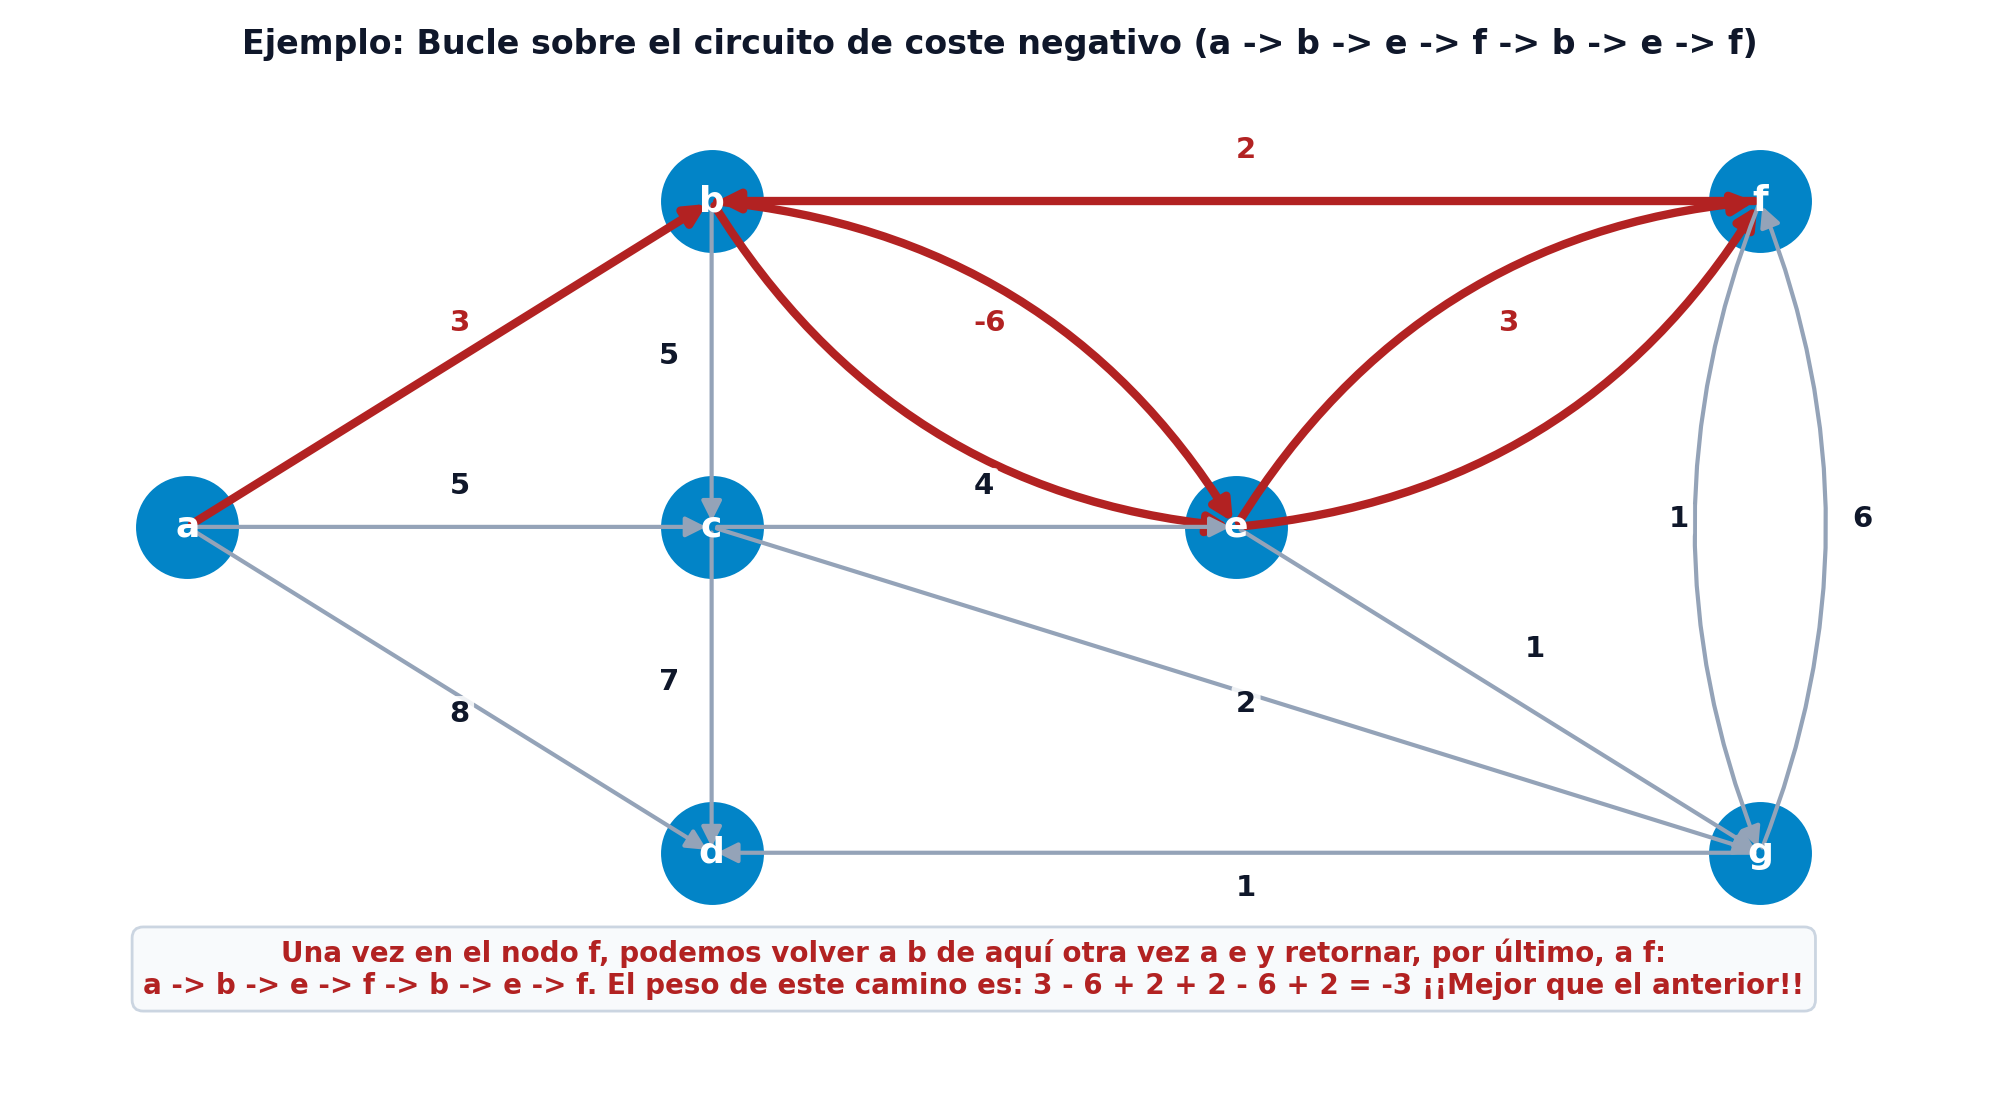
\includegraphics[width=0.75\linewidth,height=\textheight,keepaspectratio]{images/circuito_negativo_traza_paso_a_paso.png}

}

\caption{\label{fig-cminimo-circuito-negativo}Traza gráfica de la
paradoja del camino en grafos con circuitos de coste negativo}

\end{figure}%

\end{tcolorbox}

El comportamiento divergente mostrado en el ejemplo anterior evidencia
que la presencia de circuitos cerrados con coste total estrictamente
negativo impide la existencia de una solución finita. Esta propiedad
permite enunciar el teorema fundamental de existencia de solución
óptima.

\begin{tcolorbox}[enhanced jigsaw, toprule=.15mm, opacitybacktitle=0.6, coltitle=black, colbacktitle=quarto-callout-important-color!10!white, title=\textcolor{quarto-callout-important-color}{\faExclamation}\hspace{0.5em}{Teorema: Condición de existencia de solución óptima finita}, arc=.35mm, rightrule=.15mm, toptitle=1mm, breakable, bottomtitle=1mm, titlerule=0mm, colback=white, opacityback=0, leftrule=.75mm, colframe=quarto-callout-important-color-frame, left=2mm, bottomrule=.15mm]

Dada una red dirigida valorada \(G = (V, U, \mathbf{d})\) y dos vértices
fijados \(s, t \in V\), el problema de encontrar el camino mínimo entre
\(s\) y \(t\) tiene solución óptima finita si y sólo si se satisfacen
simultáneamente las siguientes dos hipótesis:

\begin{itemize}
\tightlist
\item
  \textbf{Hipótesis \(H_1\) (Accesibilidad)}: Existe al menos un camino
  dirigido en \(G\) que une el nodo origen \(s\) con el nodo destino
  \(t\).
\item
  \textbf{Hipótesis \(H_2\) (Ausencia de circuitos de coste negativo)}:
  Ningún camino dirigido de \(s\) a \(t\) contiene un circuito cuyo
  coste acumulado sea estrictamente negativo.
\end{itemize}

\emph{Demostración}: \((\implies)\) Si no se cumple \(H_1\), no existen
caminos de \(s\) a \(t\), por lo que la distancia es \(+\infty\). Si no
se cumple \(H_2\), existe un camino de \(s\) a \(t\) que atraviesa un
circuito \(\mu_C\) con \(d(\mu_C) < 0\). Recorriendo \(\mu_C\)
arbitrariamente \(k\) veces, el coste acumulado se reduce a \(-\infty\),
impidiendo la existencia de un mínimo finito.

\((\impliedby)\) Si se cumplen \(H_1\) y \(H_2\), el número de caminos
simples (elementales, sin repetición de vértices) entre \(s\) y \(t\) es
finito al ser \(|V| = n\) finito. Como todo circuito en los caminos
tiene coste \(d(\mu_C) \ge 0\), la eliminación de cualquier circuito no
incrementa la longitud del camino. Por tanto, el mínimo sobre el
conjunto finito de caminos simples es un valor real bien definido y
finito.

\end{tcolorbox}

\begin{center}\rule{0.5\linewidth}{0.5pt}\end{center}

\section{Ecuaciones de optimalidad de
Bellman}\label{ecuaciones-de-optimalidad-de-bellman}

El fundamento teórico dominante para la resolución de problemas de rutas
mínimas descansa en el \textbf{Principio de Optimalidad} formulado por
Richard E. Bellman en 1957 (Bellman 1957, 1958).

\begin{tcolorbox}[enhanced jigsaw, toprule=.15mm, opacitybacktitle=0.6, coltitle=black, colbacktitle=quarto-callout-note-color!10!white, title=\textcolor{quarto-callout-note-color}{\faInfo}\hspace{0.5em}{Principio de Optimalidad de Bellman (1957)}, arc=.35mm, rightrule=.15mm, toptitle=1mm, breakable, bottomtitle=1mm, titlerule=0mm, colback=white, opacityback=0, leftrule=.75mm, colframe=quarto-callout-note-color-frame, left=2mm, bottomrule=.15mm]

Una secuencia óptima de decisiones que resuelve un problema de
optimización multietapa debe cumplir la propiedad de que, cualquiera que
sea el estado inicial y la decisión inicial adoptada, las decisiones
restantes deben constituir una \textbf{política óptima} con respecto al
estado resultante de la primera decisión.

En el contexto de redes: \textbf{Toda subpolítica de una política óptima
es a su vez una subpolítica óptima}.

\end{tcolorbox}

La traslación de este principio a la teoría de caminos mínimos establece
que si un camino \(\mu^*[s, t]\) es de coste mínimo entre el origen
\(s\) y el destino \(t\), cualquier subcamino \(\mu^*[i, j]\) contenido
en él debe ser, de forma obligatoria, el camino de coste mínimo entre
los vértices intermedios \(i\) y \(j\).

Denotemos por \(u_{ij}\) la longitud del camino mínimo entre los
vértices \(i\) y \(j\). Para cualquier par \(s, t \in V\), la distancia
óptima satisface la relación de consistencia:

\[
u_{st} = \min_{i, j \in V} \{ u_{si} + u_{ij} + u_{jt} \}
\]

En particular, si fijamos un origen único \(s = 1\) y denotamos por
\(u_j \equiv u_{1j}\) a la distancia mínima desde el origen \(1\) al
nodo \(j \in V\), podemos descomponer la última etapa identificando el
predecesor directo \(i\) del nodo \(j\), obteniendo el sistema
fundamental de ecuaciones de optimalidad.

\begin{tcolorbox}[enhanced jigsaw, toprule=.15mm, opacitybacktitle=0.6, coltitle=black, colbacktitle=quarto-callout-important-color!10!white, title=\textcolor{quarto-callout-important-color}{\faExclamation}\hspace{0.5em}{Ecuaciones de optimalidad de Bellman}, arc=.35mm, rightrule=.15mm, toptitle=1mm, breakable, bottomtitle=1mm, titlerule=0mm, colback=white, opacityback=0, leftrule=.75mm, colframe=quarto-callout-important-color-frame, left=2mm, bottomrule=.15mm]

Dada una red dirigida valorada \(G = (V, U, \mathbf{d})\) sin circuitos
de coste negativo, las distancias mínimas \(u_j\) desde el nodo origen
\(1\) a cada uno de los demás nodos \(j \in V \setminus \{1\}\)
satisfacen el sistema de ecuaciones no lineales:

\[
\begin{aligned}
u_1 &= 0 \\
u_j &= \min_{k \neq j} \{ u_k + d_{kj} \}, \quad \forall j = 2, \dots, n
\end{aligned}
\]

Donde \(d_{kj}\) son las componentes de la matriz de distancias directas
\(D\).

\end{tcolorbox}

Las ecuaciones de optimalidad de Bellman identifican las condiciones
necesarias que deben verificar las distancias mínimas \(u_j\) desde un
vértice origen a todos los demás nodos de la red. Físicamente,
establecen que la longitud del camino mínimo hasta cualquier nodo \(j\)
equivale al mínimo entre las distancias acumuladas a sus predecesores
directos \(k\) más el coste del arco de entrada \((k, j)\). Sin embargo,
por sí solas, estas ecuaciones presentan dos limitaciones fundamentales:
no indican el orden secuencial en el que deben resolverse los nodos (lo
que en redes generales exigiría explorar \(O(n!)\) combinaciones) y no
garantizan la unicidad de solución en presencia de circuitos de coste
nulo o negativo.

Para observar el funcionamiento analítico de este sistema, examinemos un
primer ejemplo numérico sobre un digrafo de 5 nodos.

\begin{tcolorbox}[enhanced jigsaw, toprule=.15mm, opacitybacktitle=0.6, coltitle=black, colbacktitle=quarto-callout-tip-color!10!white, title=\textcolor{quarto-callout-tip-color}{\faLightbulb}\hspace{0.5em}{Ejemplo: Planteamiento y resolución de las ecuaciones de Bellman}, arc=.35mm, rightrule=.15mm, toptitle=1mm, breakable, bottomtitle=1mm, titlerule=0mm, colback=white, opacityback=0, leftrule=.75mm, colframe=quarto-callout-tip-color-frame, left=2mm, bottomrule=.15mm]

Consideremos el digrafo valorado de 5 nodos presentado en la
Figura~\ref{fig-bellman-ecuaciones-ejemplo}. Se desea formular las
ecuaciones de Bellman y determinar la distancia mínima desde el nodo 1
al resto de los vértices.

\begin{figure}[H]

\centering{

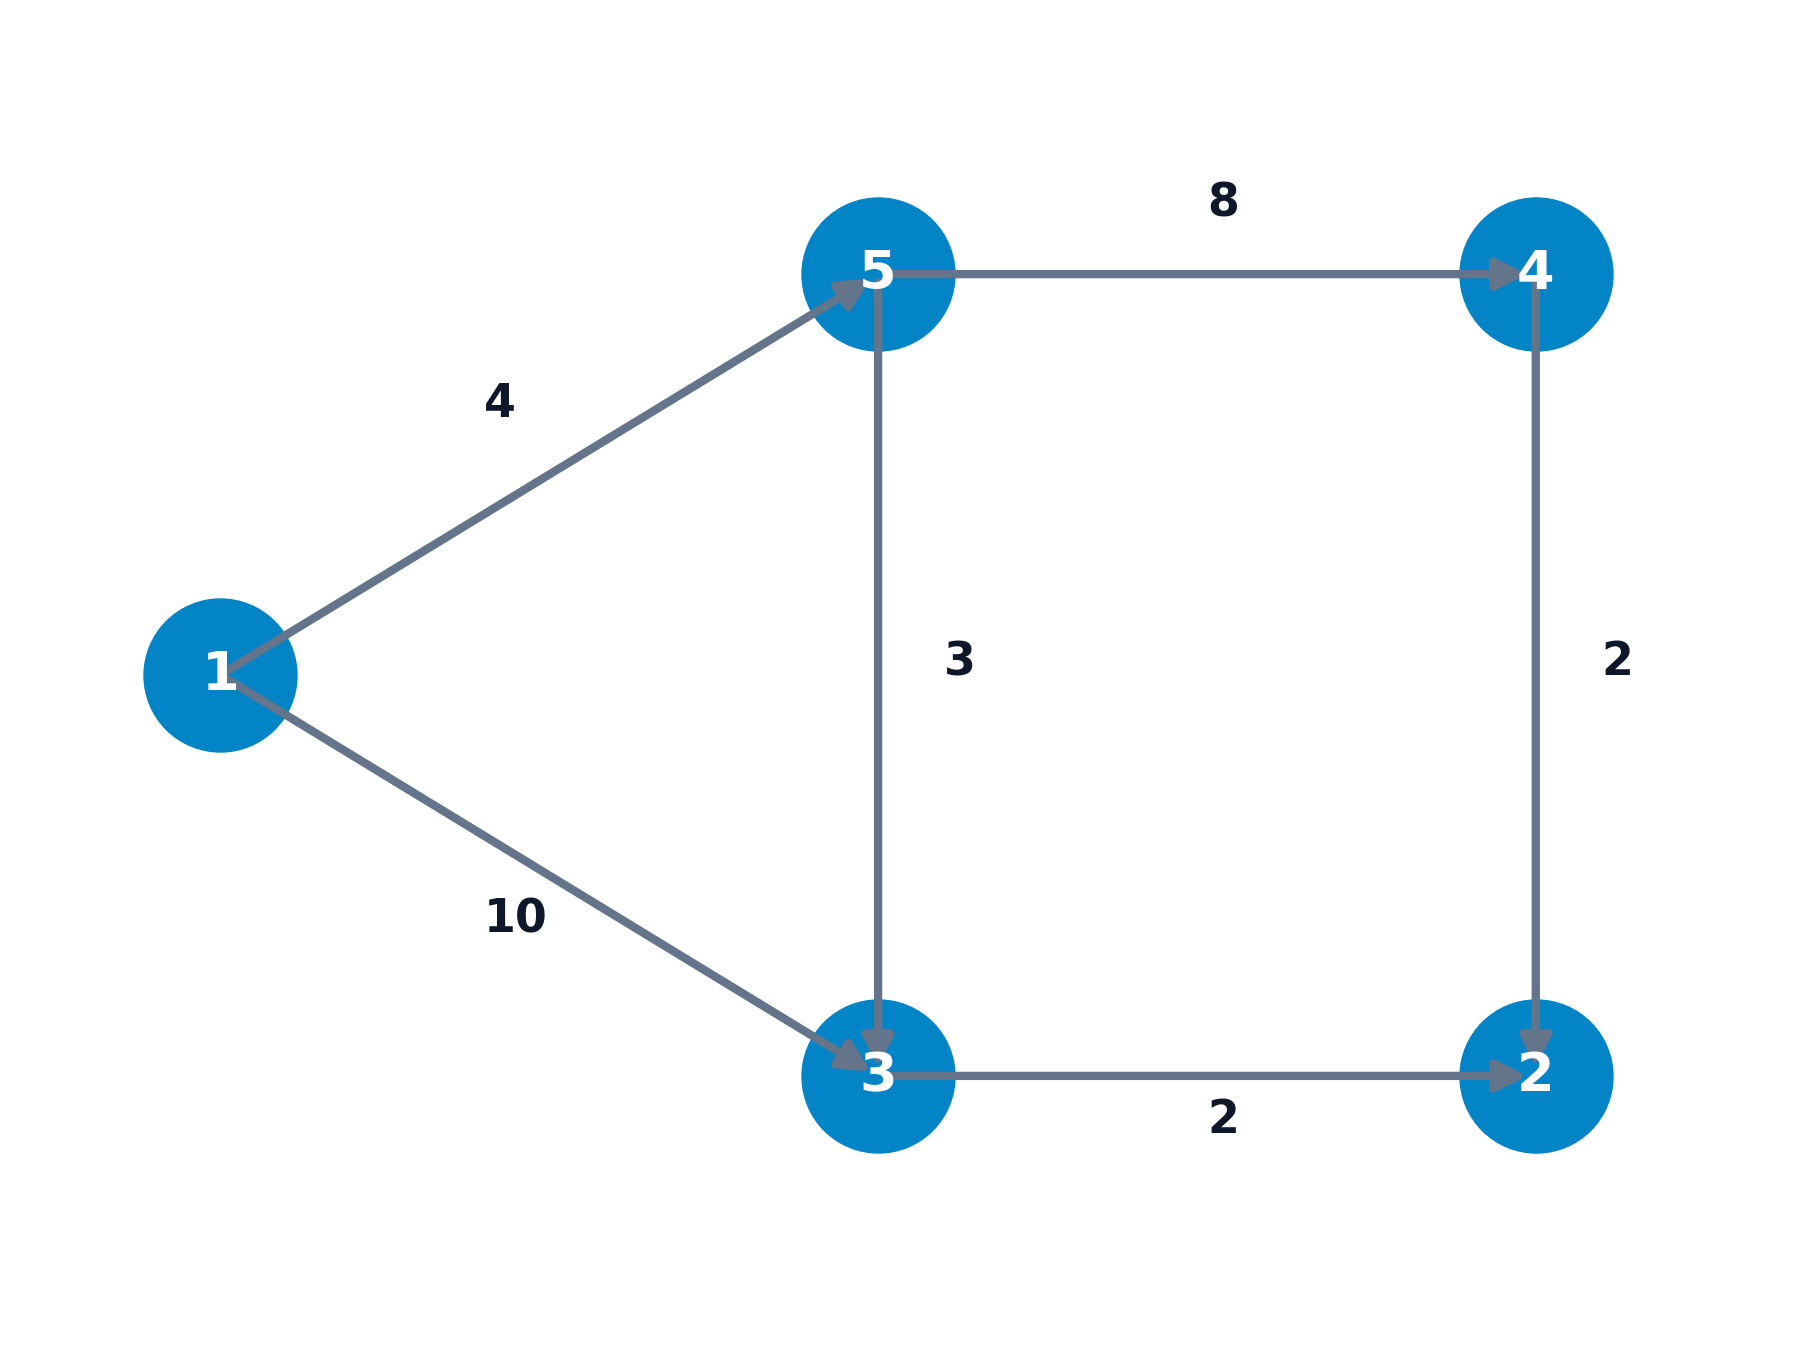
\includegraphics[width=0.65\linewidth,height=\textheight,keepaspectratio]{images/bellman_ecuaciones_ejemplo.png}

}

\caption{\label{fig-bellman-ecuaciones-ejemplo}Digrafo valorado de 5
nodos para la formulación de las ecuaciones de Bellman}

\end{figure}%

El sistema de ecuaciones de Bellman para el origen \(s = 1\) se plantea
expresando la etiqueta de cada nodo en función del mínimo de sus
predecesores directos:

\[
\begin{aligned}
u_1 &= 0 \\
u_5 &= \min \{ u_1 + d_{15} \} = \min \{ 0 + 4 \} = 4 \\
u_3 &= \min \{ u_1 + d_{13}, u_5 + d_{53} \} = \min \{ 0 + 10, 4 + 3 \} = \min \{ 10, 7 \} = 7 \\
u_4 &= \min \{ u_5 + d_{54} \} = \min \{ 4 + 8 \} = 12 \\
u_2 &= \min \{ u_3 + d_{32}, u_4 + d_{42} \} = \min \{ 7 + 2, 12 + 2 \} = \min \{ 9, 14 \} = 9
\end{aligned}
\]

Al resolver consecutivamente el sistema, se obtienen las distancias
geodésicas y la arborescencia óptima:

\begin{itemize}
\tightlist
\item
  \textbf{Vector de distancias mínimas}:
  \(\mathbf{u} = (u_1, u_2, u_3, u_4, u_5) = (0, 9, 7, 12, 4)\).
\item
  \textbf{Vector de predecesores}: \(\text{Pred} = (1, 3, 5, 5, 1)\).
\item
  \textbf{Arborescencia de caminos mínimos}:
  \(\{ (1,5), (5,3), (5,4), (3,2) \}\).
\end{itemize}

\end{tcolorbox}

A pesar de su claridad teórica, es crucial recalcar que las ecuaciones
de Bellman constituyen una \textbf{condición necesaria} de optimalidad,
pero no siempre suficiente. En particular, si la red contiene circuitos
cerrados con coste nulo (\(d(\mu_C) = 0\)), el sistema algebraico admite
múltiples soluciones, de las cuales solo una representa las verdaderas
distancias mínimas.

\begin{tcolorbox}[enhanced jigsaw, toprule=.15mm, opacitybacktitle=0.6, coltitle=black, colbacktitle=quarto-callout-tip-color!10!white, title=\textcolor{quarto-callout-tip-color}{\faLightbulb}\hspace{0.5em}{Ejemplo: No unicidad de solución por presencia de circuito de coste nulo}, arc=.35mm, rightrule=.15mm, toptitle=1mm, breakable, bottomtitle=1mm, titlerule=0mm, colback=white, opacityback=0, leftrule=.75mm, colframe=quarto-callout-tip-color-frame, left=2mm, bottomrule=.15mm]

Consideremos el digrafo de 3 nodos mostrado en la
Figura~\ref{fig-cminimo-circuito-nulo}, con arcos \((1, 2)\) de peso 10,
\((2, 3)\) de peso \(1\) y \((3, 2)\) de peso \(-1\). El circuito
formado por los nodos 2 y 3 posee un coste total
\(d_{23} + d_{32} = 1 + (-1) = 0\).

El sistema de ecuaciones de Bellman para el origen \(s = 1\) es:

\[
\begin{aligned}
u_1 &= 0 \\
u_2 &= \min \{ u_1 + d_{12}, u_3 + d_{32} \} = \min \{ 0 + 10, u_3 - 1 \} \\
u_3 &= \min \{ u_1 + d_{13}, u_2 + d_{23} \} = \min \{ 0 + \infty, u_2 + 1 \} = u_2 + 1
\end{aligned}
\]

Todo vector \((u_1, u_2, u_3)\) que satisfaga la relación \(u_1 = 0\),
\(u_2 \le 10\) y \(u_3 = u_2 + 1\) constituye una solución matemática
del sistema:

\begin{itemize}
\tightlist
\item
  Si fijamos \(u_2 = 10 \implies u_3 = 11\). Este vector \((0, 10, 11)\)
  identifica la distancia mínima real.
\item
  Sin embargo, el vector arbitrario \((0, 5, 6)\) también satisface el
  sistema algebraico (\(5 = \min\{10, 6-1\} = 5\) y \(6 = 5+1\)), pero
  \textbf{no representa las distancias mínimas}.
\end{itemize}

\begin{figure}[H]

\centering{

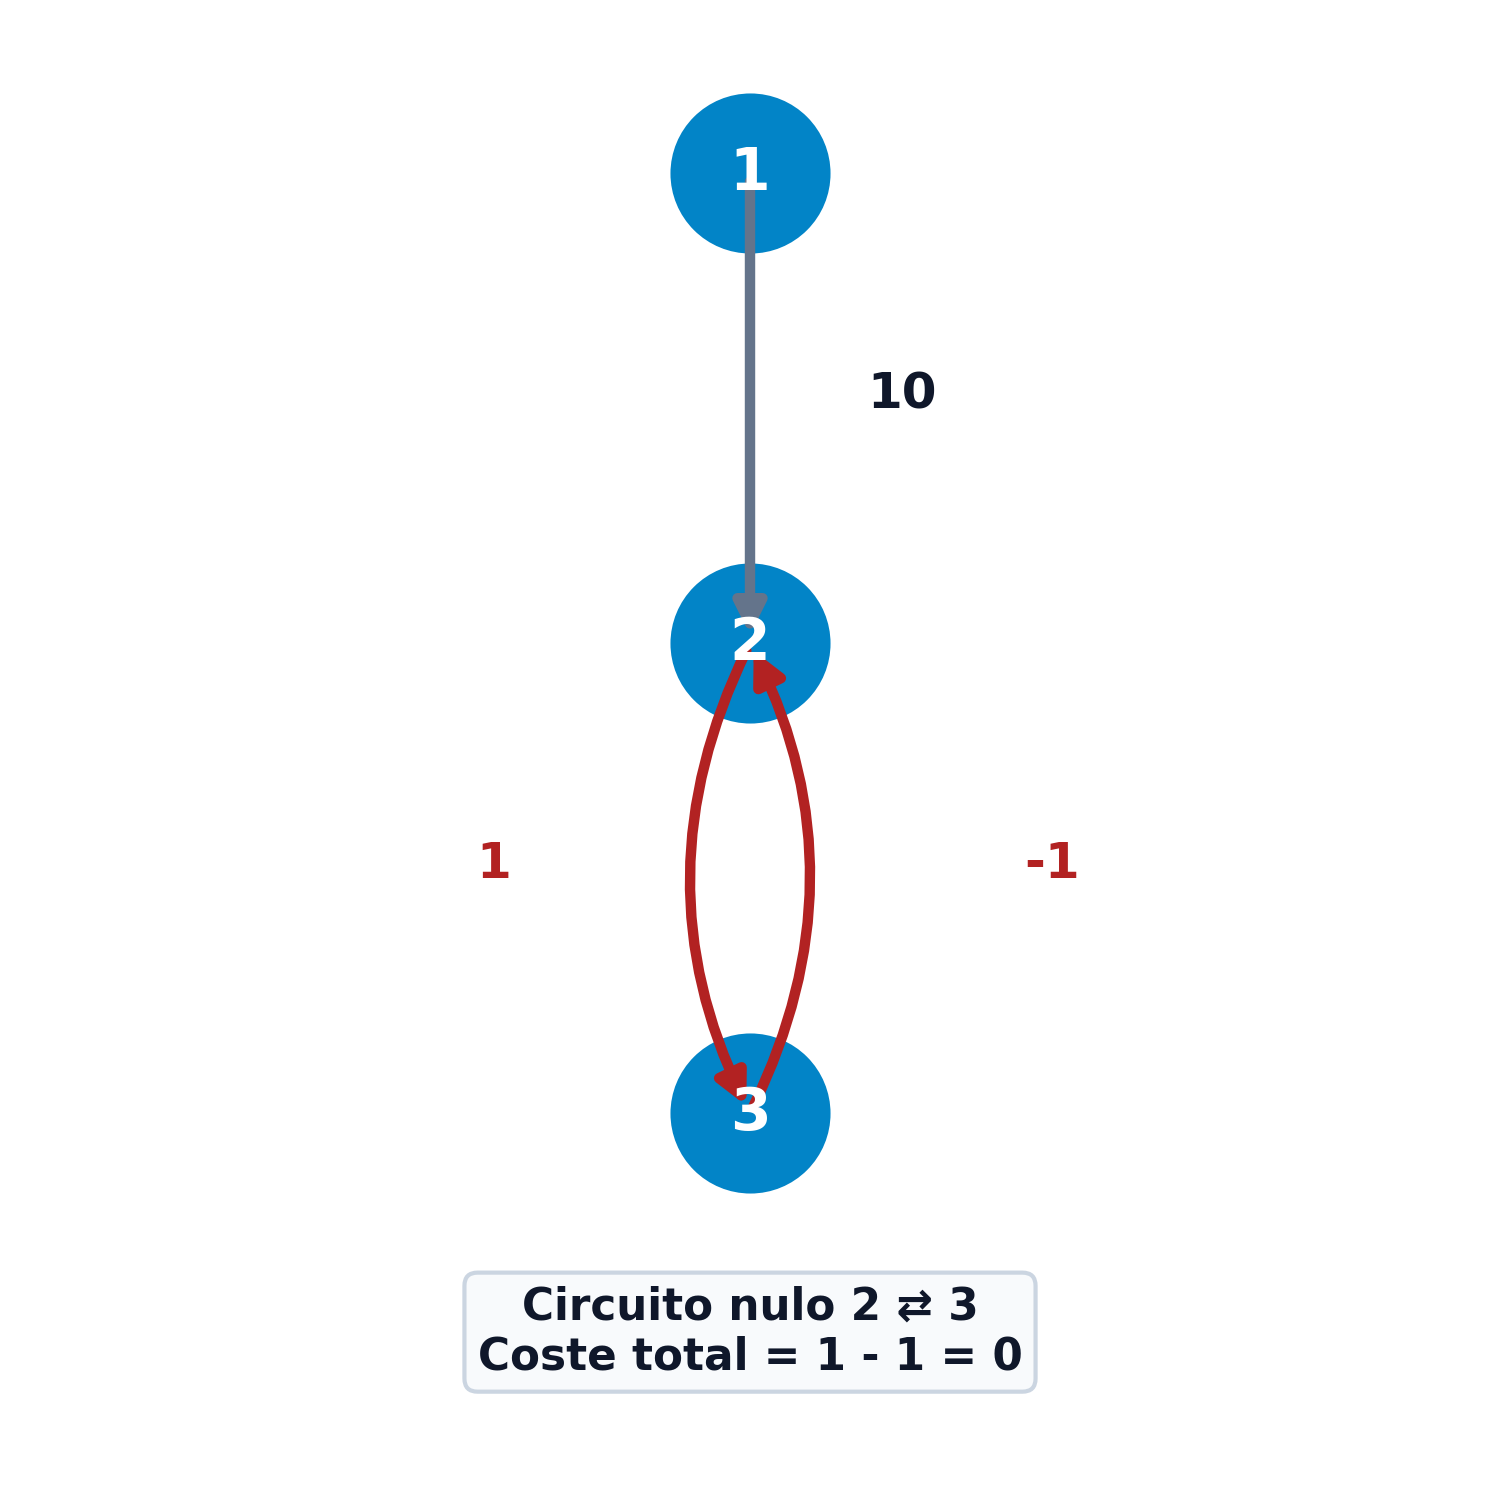
\includegraphics[width=0.55\linewidth,height=\textheight,keepaspectratio]{images/cminimo_circuito_nulo.png}

}

\caption{\label{fig-cminimo-circuito-nulo}Digrafo con un circuito de
coste nulo que provoca la existencia de soluciones algebraicas no únicas
en Bellman}

\end{figure}%

\end{tcolorbox}

Para garantizar que las ecuaciones de Bellman determinen de forma única
las distancias geodésicas y permitan construir la arborescencia soporte
de caminos mínimos, se exige la ausencia estricta de circuitos dirigidos
de coste nulo o negativo.

\begin{tcolorbox}[enhanced jigsaw, toprule=.15mm, opacitybacktitle=0.6, coltitle=black, colbacktitle=quarto-callout-note-color!10!white, title=\textcolor{quarto-callout-note-color}{\faInfo}\hspace{0.5em}{Proposición: Construcción de la arborescencia asociada a las ecuaciones
de Bellman}, arc=.35mm, rightrule=.15mm, toptitle=1mm, breakable, bottomtitle=1mm, titlerule=0mm, colback=white, opacityback=0, leftrule=.75mm, colframe=quarto-callout-note-color-frame, left=2mm, bottomrule=.15mm]

Las ecuaciones de optimalidad de Bellman:

\[
\begin{aligned}
u_1 &= 0 \\
u_j &= \min_{k \neq j} \{ u_k + d_{kj} \}, \quad \forall j \neq 1
\end{aligned}
\]

permiten construir de forma única la \textbf{arborescencia de caminos
mínimos} con raíz en el origen 1 si y sólo si en la red no existen
circuitos dirigidos de longitud o coste nulo ni negativo.

\end{tcolorbox}

Apliquemos nuevamente esta proposición al problema planteado en la red
de aeropuertos para verificar la construcción analítica de sus rutas
óptimas.

\begin{tcolorbox}[enhanced jigsaw, toprule=.15mm, opacitybacktitle=0.6, coltitle=black, colbacktitle=quarto-callout-tip-color!10!white, title=\textcolor{quarto-callout-tip-color}{\faLightbulb}\hspace{0.5em}{Ejemplo: Planteamiento de las ecuaciones de Bellman en el problema de la
red de aeropuertos}, arc=.35mm, rightrule=.15mm, toptitle=1mm, breakable, bottomtitle=1mm, titlerule=0mm, colback=white, opacityback=0, leftrule=.75mm, colframe=quarto-callout-tip-color-frame, left=2mm, bottomrule=.15mm]

Consideremos el problema de la red de aeropuertos presentado en la
Figura~\ref{fig-cminimo-ejemplo-vuelos}, con el origen fijado en el
aeropuerto de Madrid (\(M\)). Se desea formular las ecuaciones de
Bellman y obtener el camino mínimo desde el nodo \(M\) a todos los demás
destinos.

El sistema de ecuaciones de Bellman se plantea evaluando la etiqueta de
cada aeropuerto como el mínimo sobre todos sus vuelos de llegada
directos:

\[
\begin{aligned}
u_M &= 0 \\
u_L &= \min \{ u_M + d_{ML} \} = \min \{ 0 + 20 \} = 20 \\
u_P &= \min \{ u_M + d_{MP}, u_F + d_{FP} \} = \min \{ 0 + 27, 30 + 9 \} = 27 \\
u_F &= \min \{ u_M + d_{MF}, u_L + d_{LF}, u_P + d_{PF} \} \\
    &= \min \{ 0 + 40, 20 + 10, 27 + 11 \} = \min \{ 40, 30, 38 \} = 30 \\
u_S &= \min \{ u_F + d_{FS}, u_P + d_{PS} \} = \min \{ 30 + 90, 27 + 100 \} = \min \{ 120, 127 \} = 120 \\
u_T &= \min \{ u_P + d_{PT}, u_S + d_{ST} \} = \min \{ 27 + 150, 120 + 35 \} = \min \{ 177, 155 \} = 155
\end{aligned}
\]

La resolución directa del sistema proporciona las siguientes soluciones:

\begin{itemize}
\tightlist
\item
  \textbf{Vector de distancias mínimas}:
  \(\mathbf{u} = (u_M, u_L, u_F, u_P, u_S, u_T) = (0, 20, 30, 27, 120, 155)\).
\item
  \textbf{Arborescencia de rutas óptimas}: Integrada por las
  trayectorias \(M \to L\) (Londres: 20), \(M \to P\) (París: 27),
  \(M \to L \to F\) (Frankfurt: 30), \(M \to L \to F \to S\) (Singapur:
  120) y \(M \to L \to F \to S \to T\) (Tokio: 155).
\end{itemize}

\end{tcolorbox}

Finalmente, debemos reflexionar sobre la complejidad computacional
asociada a la resolución práctica de las ecuaciones de Bellman:

\begin{itemize}
\tightlist
\item
  \textbf{Complejidad factorial \(O(n!)\)}: Sin conocer de antemano el
  orden en el que deben resolverse los vértices, evaluar el sistema
  explorando todas las secuencias posibles de predecesores requiere un
  esfuerzo combinatorio de \(O(n!)\).
\item
  \textbf{Reducción de complejidad mediante ordenación topológica}: Si
  se logra establecer una ordenación adecuada de los nodos, la
  complejidad de resolución del sistema de Bellman se reduce
  drásticamente a \(O(n^2)\) (o tiempo estrictamente lineal
  \(O(|V| + |U|)\)) más el coste del algoritmo de ordenación.
\item
  \textbf{Restricción de aciclicidad}: Dicha ordenación topológica
  secuencial \textbf{únicamente es posible si el grafo no contiene
  circuitos dirigidos} (Grafos Dirigidos Acíclicos o DAGs).
\end{itemize}

\begin{center}\rule{0.5\linewidth}{0.5pt}\end{center}

\section{Redes sin circuitos (DAGs) y ordenación
topológica}\label{redes-sin-circuitos-dags-y-ordenaciuxf3n-topoluxf3gica}

Cuando una red dirigida no contiene circuitos cerrados (\emph{Directed
Acyclic Graph}, DAG), su estructura topológica permite ordenar los
vértices de manera secuencial. Esta propiedad resulta determinante, pues
transforma el complejo sistema no lineal de ecuaciones de Bellman en una
sucesión de cálculos directos en tiempo \textbf{estrictamente lineal}
\(O(|V| + |U|)\).

\begin{tcolorbox}[enhanced jigsaw, toprule=.15mm, opacitybacktitle=0.6, coltitle=black, colbacktitle=quarto-callout-note-color!10!white, title=\textcolor{quarto-callout-note-color}{\faInfo}\hspace{0.5em}{Proposición: Caracterización de digrafos acíclicos mediante ordenación
topológica}, arc=.35mm, rightrule=.15mm, toptitle=1mm, breakable, bottomtitle=1mm, titlerule=0mm, colback=white, opacityback=0, leftrule=.75mm, colframe=quarto-callout-note-color-frame, left=2mm, bottomrule=.15mm]

Un digrafo \(G = (V, U)\) no tiene circuitos dirigidos (es un DAG) si y
sólo si existe una \textbf{ordenación o numeración topológica} de sus
\(n\) vértices \(v_1, v_2, \dots, v_n\) tal que para todo arco dirigido
\((i, j) \in U\) se cumple la condición estricta de orden:

\[
i < j
\]

\end{tcolorbox}

\begin{tcolorbox}[enhanced jigsaw, toprule=.15mm, opacitybacktitle=0.6, coltitle=black, colbacktitle=quarto-callout-tip-color!10!white, title=\textcolor{quarto-callout-tip-color}{\faLightbulb}\hspace{0.5em}{Ejemplo: Verificación de la propiedad de ordenación topológica}, arc=.35mm, rightrule=.15mm, toptitle=1mm, breakable, bottomtitle=1mm, titlerule=0mm, colback=white, opacityback=0, leftrule=.75mm, colframe=quarto-callout-tip-color-frame, left=2mm, bottomrule=.15mm]

Consideremos nuevamente el digrafo de 5 nodos presentado en la
Figura~\ref{fig-bellman-ecuaciones-ejemplo}. En dicho grafo, los
vértices pueden disponerse en la secuencia de ordenación topológica
\((1, 5, 3, 4, 2)\).

Al examinar individualmente cada uno de los arcos dirigidos existentes
en la red:

\begin{itemize}
\tightlist
\item
  \((1, 5) \implies 1^\circ \text{ precede a } 2^\circ\) (cumple
  \(i < j\)).
\item
  \((1, 3) \implies 1^\circ \text{ precede a } 3^\circ\) (cumple
  \(i < j\)).
\item
  \((5, 4) \implies 2^\circ \text{ precede a } 4^\circ\) (cumple
  \(i < j\)).
\item
  \((5, 3) \implies 2^\circ \text{ precede a } 3^\circ\) (cumple
  \(i < j\)).
\item
  \((4, 2) \implies 4^\circ \text{ precede a } 5^\circ\) (cumple
  \(i < j\)).
\item
  \((3, 2) \implies 3^\circ \text{ precede a } 5^\circ\) (cumple
  \(i < j\)).
\end{itemize}

Puesto que todos los arcos avanzan estrictamente de izquierda a derecha
sin la presencia de arcos de retroceso, se confirma que la secuencia de
numeración satisface rigurosamente la propiedad de aciclicidad.

\end{tcolorbox}

Para determinar esta numeración de manera sistemática en cualquier red
acíclica, se ejecuta el siguiente algoritmo basado en la eliminación
sucesiva de nodos fuentes (nodos sin arcos de entrada).

\begin{tcolorbox}[enhanced jigsaw, toprule=.15mm, opacitybacktitle=0.6, coltitle=black, colbacktitle=quarto-callout-note-color!10!white, title=\textcolor{quarto-callout-note-color}{\faInfo}\hspace{0.5em}{Esquema: Algoritmo de numeración y ordenación topológica}, arc=.35mm, rightrule=.15mm, toptitle=1mm, breakable, bottomtitle=1mm, titlerule=0mm, colback=white, opacityback=0, leftrule=.75mm, colframe=quarto-callout-note-color-frame, left=2mm, bottomrule=.15mm]

Dada una red dirigida \(G = (V, U)\) con \(n = |V|\) vértices:

\begin{enumerate}
\def\labelenumi{\arabic{enumi}.}
\tightlist
\item
  \textbf{Paso 0 (Inicialización)}:

  \begin{itemize}
  \tightlist
  \item
    Hacer \(k \leftarrow 1\) y \(V' \leftarrow V, U' \leftarrow U\).
  \end{itemize}
\item
  \textbf{Paso 1 (Selección de nodo fuente)}:

  \begin{itemize}
  \tightlist
  \item
    Seleccionar un nodo \(i \in V'\) al que no llegue ningún arco en
    \(U'\) (grado de entrada \(d^-(i) = 0\)). En un digrafo acíclico
    siempre existe al menos un nodo fuente.
  \end{itemize}
\item
  \textbf{Paso 2 (Asignación y eliminación)}:

  \begin{itemize}
  \tightlist
  \item
    Asignar al nodo \(i\) el número de orden topológico \(k\).
  \item
    Eliminar el nodo \(i\) y todos los arcos que inciden en él:
    \(V' \leftarrow V' \setminus \{i\}\),
    \(U' \leftarrow U' \setminus \{ (i, j) \in U' \}\).
  \end{itemize}
\item
  \textbf{Paso 3 (Criterio de Parada)}:

  \begin{itemize}
  \tightlist
  \item
    Si \(k = n\), detener el procedimiento (se han numerado todos los
    nodos).
  \item
    En otro caso, hacer \(k \leftarrow k + 1\) y regresar al Paso 1.
  \end{itemize}
\end{enumerate}

\end{tcolorbox}

Una vez que la red ha sido ordenada topológicamente de modo que los
arcos cumplan \(i < j\), la resolución del sistema de ecuaciones de
Bellman se vuelve \textbf{completamente trivial y directa}. No es
necesario realizar iteraciones aproximadas ni resolver sistemas de
ecuaciones simultáneas: basta con calcular secuencialmente la etiqueta
de distancia mínima \(u_j\) de cada nodo \(j = 2, \dots, n\) evaluando a
sus predecesores directos \(i < j\) que ya han sido resueltos
previamente:

\[
\begin{aligned}
u_1 &= 0 \\
u_j &= \min_{i < j, \, (i, j) \in U} \{ u_i + d_{ij} \}, \quad \forall j = 2, \dots, n
\end{aligned}
\]

Puesto que cada arco de la red se examina exactamente una vez durante
este recorrido secuencial de izquierda a derecha, la complejidad
algorítmica total es \textbf{estrictamente lineal \(O(|V| + |U|)\)}.

\begin{tcolorbox}[enhanced jigsaw, toprule=.15mm, opacitybacktitle=0.6, coltitle=black, colbacktitle=quarto-callout-tip-color!10!white, title=\textcolor{quarto-callout-tip-color}{\faLightbulb}\hspace{0.5em}{Ejemplo: Resolución de las ecuaciones de Bellman en un DAG de 7 nodos}, arc=.35mm, rightrule=.15mm, toptitle=1mm, breakable, bottomtitle=1mm, titlerule=0mm, colback=white, opacityback=0, leftrule=.75mm, colframe=quarto-callout-tip-color-frame, left=2mm, bottomrule=.15mm]

Consideremos el digrafo acíclico de 7 nodos presentado en la
Figura~\ref{fig-dag-ejemplo-7nodos}, cuyos vértices ya están numerados
respetando el orden topológico \(i < j\). Se desea calcular las
distancias mínimas desde el origen \(s = 1\) a todos los vértices de la
red.

Evaluando las ecuaciones de Bellman en orden topológico creciente de
\(j = 1\) a \(7\):

\begin{itemize}
\tightlist
\item
  \textbf{Nodo 1 (Origen)}: \(u_1 = 0\).
\item
  \textbf{Nodo 2} (Predecesores \(\{1\}\)):
  \[u_2 = u_1 + d_{12} = 0 + 3 = 3 \implies \text{Pred}(2) = 1\]
\item
  \textbf{Nodo 3} (Predecesores \(\{1, 2\}\)):
  \[u_3 = \min \{ u_1 + d_{13}, u_2 + d_{23} \} = \min \{ 0 + 5, 3 + 5 \} = 5 \implies \text{Pred}(3) = 1\]
\item
  \textbf{Nodo 4} (Predecesores \(\{2, 3\}\)):
  \[u_4 = \min \{ u_2 + d_{24}, u_3 + d_{34} \} = \min \{ 3 - 6, 5 + 4 \} = -3 \implies \text{Pred}(4) = 2\]
\item
  \textbf{Nodo 5} (Predecesores \(\{2, 4\}\)):
  \[u_5 = \min \{ u_2 + d_{25}, u_4 + d_{45} \} = \min \{ 3 + 2, -3 + 2 \} = -1 \implies \text{Pred}(5) = 4\]
\item
  \textbf{Nodo 6} (Predecesores \(\{3, 4, 5\}\)):
  \[u_6 = \min \{ u_3 + d_{36}, u_4 + d_{46}, u_5 + d_{56} \} = \min \{ 5 + 2, -3 + 3, -1 + 6 \} = 0 \implies \text{Pred}(6) = 4\]
\item
  \textbf{Nodo 7} (Predecesores \(\{1, 3, 6\}\)):
  \[u_7 = \min \{ u_1 + d_{17}, u_3 + d_{37}, u_6 + d_{67} \} = \min \{ 0 + 8, 5 + 7, 0 + 1 \} = 1 \implies \text{Pred}(7) = 6\]
\end{itemize}

\begin{figure}[H]

\centering{

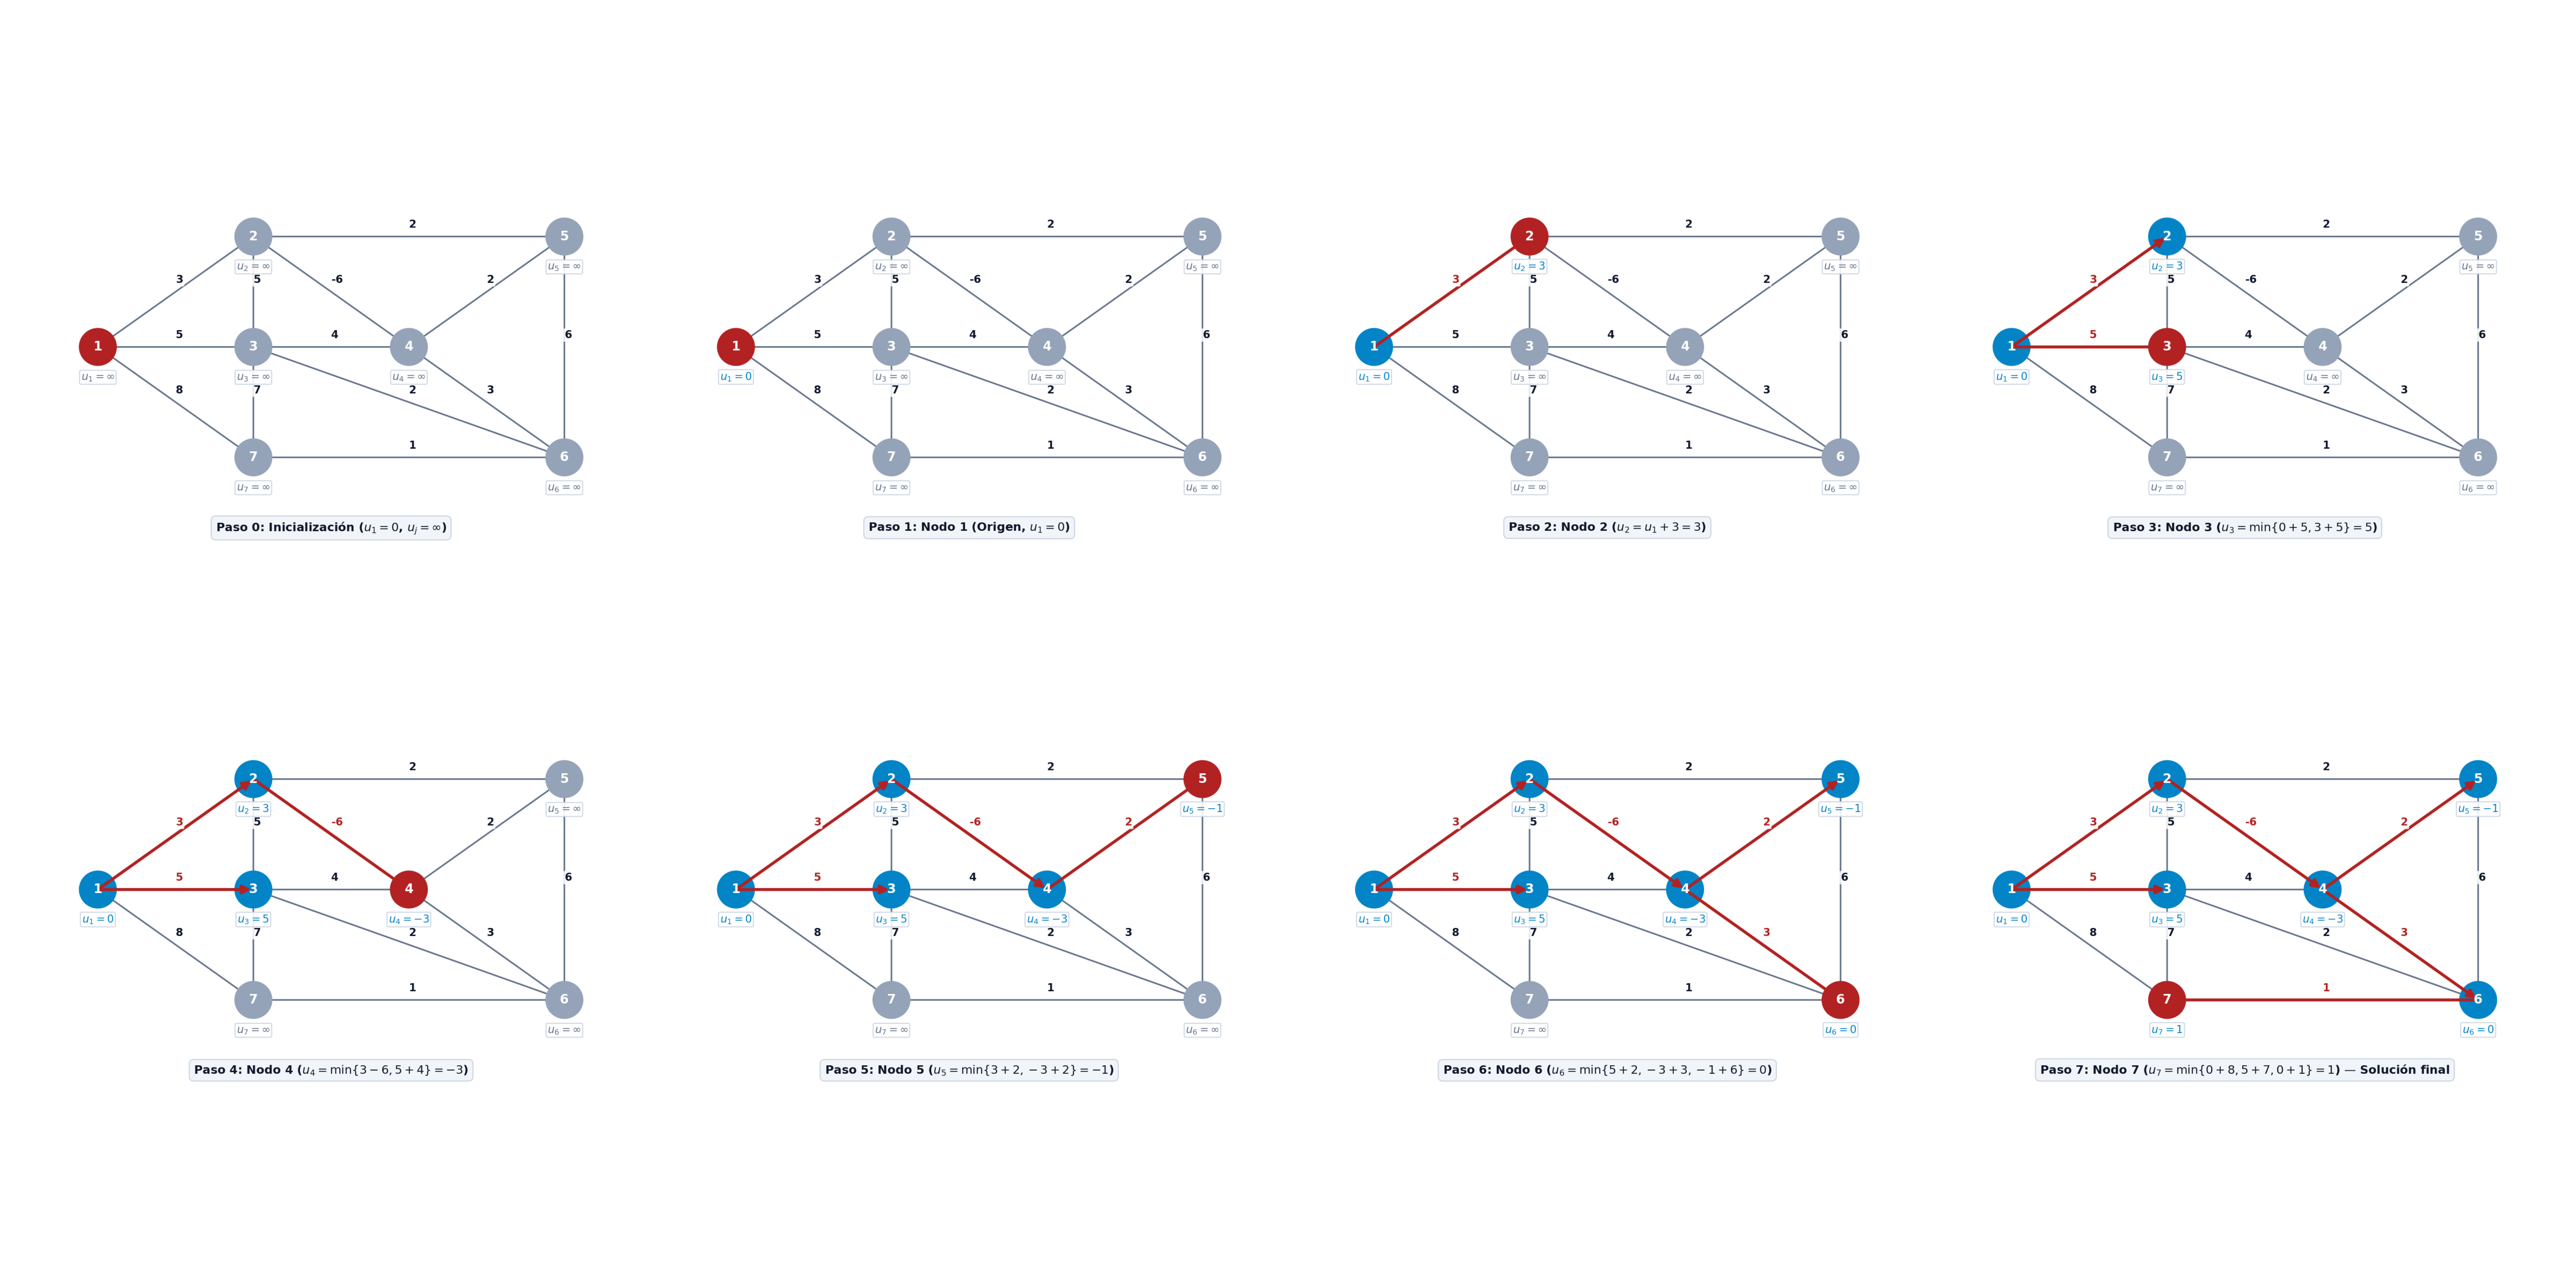
\includegraphics[width=0.8\linewidth,height=\textheight,keepaspectratio]{images/dag_ejemplo_7nodos_traza_paso_a_paso.png}

}

\caption{\label{fig-dag-ejemplo-7nodos}Traza completa paso a paso del
algoritmo de Bellman en un DAG de 7 nodos}

\end{figure}%

Al resolver consecutivamente el sistema, obtenemos los siguientes
resultados:

El vector de distancias mínimas es
\(\mathbf{u} = (u_1, u_2, u_3, u_4, u_5, u_6, u_7) = (0, 3, 5, -3, -1, 0, 1)\),
mientras que el vector de predecesores resulta ser
\(\text{Pred} = (1, 1, 1, 2, 4, 4, 6)\). Finalmente, la arborescencia de
caminos mínimos queda conformada por las aristas dirigidas
\(\{ (1,2), (1,3), (2,4), (4,5), (4,6), (6,7) \}\).

\end{tcolorbox}

\begin{center}\rule{0.5\linewidth}{0.5pt}\end{center}

\section{Redes con pesos no negativos: Algoritmo de
Dijkstra}\label{redes-con-pesos-no-negativos-algoritmo-de-dijkstra}

Para redes dirigidas generales en las que las longitudes de todos los
arcos son estrictamente no negativas (\(d_{ij} \ge 0\)), el
procedimiento de origen único más eficiente y célebre es el
\textbf{Algoritmo de Dijkstra}, introducido por Edsger W. Dijkstra en
1959 (Dijkstra 1959).

El fundamento conceptual de esta técnica reside en su naturaleza de
algoritmo \textbf{voraz} (\emph{greedy}) basado en un mecanismo de
etiquetado permanente. A diferencia de otros enfoques exploratorios que
requieren múltiples pasadas sobre el grafo, el algoritmo de Dijkstra
construye la solución óptima acumulativamente: en cada etapa, fija la
distancia geodésica definitiva desde el origen \(1\) hacia exactamente
un nuevo nodo de la red, garantizando que el problema quede resuelto por
completo tras un máximo de \(n - 1\) iteraciones.

\begin{tcolorbox}[enhanced jigsaw, toprule=.15mm, opacitybacktitle=0.6, coltitle=black, colbacktitle=quarto-callout-note-color!10!white, title=\textcolor{quarto-callout-note-color}{\faInfo}\hspace{0.5em}{Definición: Subconjuntos de etiquetado y cota de distancia \(u_j^P\)}, arc=.35mm, rightrule=.15mm, toptitle=1mm, breakable, bottomtitle=1mm, titlerule=0mm, colback=white, opacityback=0, leftrule=.75mm, colframe=quarto-callout-note-color-frame, left=2mm, bottomrule=.15mm]

En la etapa \(k\) de la ejecución del Algoritmo de Dijkstra, los
vértices del grafo \(V\) se dividen dinámicamente en dos subconjuntos
disjuntos:

\begin{enumerate}
\def\labelenumi{\arabic{enumi}.}
\tightlist
\item
  \textbf{Conjunto de nodos permanentes \(\mathcal{P} \subset V\)}:
  Agrupa a los \(k\) vértices (con \(1 \in \mathcal{P}\)) para los
  cuales ya se conoce de forma exacta su distancia mínima desde el
  origen. Para todo nodo \(j \in \mathcal{P}\), la etiqueta \(u_j\) es
  exactamente igual al valor óptimo \(d(1, j)\).
\item
  \textbf{Conjunto de nodos transitorios
  \(\mathcal{T} = V \setminus \mathcal{P}\)}: Agrupa a los vértices
  restantes para los cuales la etiqueta \(u_j\) representa únicamente
  una cota superior provisional del camino mínimo.
\end{enumerate}

Dado este subconjunto \(\mathcal{P}\), la cota provisional \(u_j^P\)
asociada a un nodo \(j \in V\) se define como la longitud del camino
mínimo desde el origen \(1\) al nodo \(j\) restringido a utilizar como
vértices intermedios \textbf{únicamente elementos pertenecientes a
\(\mathcal{P}\)}:

\[
u_j^P \equiv \text{longitud del camino mínimo de } 1 \text{ a } j \text{ con vértices intermedios en } \mathcal{P}
\]

\end{tcolorbox}

El procedimiento práctico comienza fijando el nodo origen en el conjunto
permanente (\(\mathcal{P} = \{1\}\) con \(u_1 = 0\)) y asignando a los
restantes vértices transitorios \(j \in \mathcal{T} = \{2, \dots, n\}\)
la distancia del arco directo de entrada \(u_j = d_{1j}\), asumiendo
\(d_{1j} = +\infty\) si el nodo \(j\) no posee conexión directa desde el
origen.

A partir de esta configuración inicial, cada iteración del algoritmo
desarrolla dos fases consecutivas de cálculo. En primer lugar, la
\textbf{fase de selección voraz} identifica el nodo transitorio
\(j^* \in \mathcal{T}\) que posee la etiqueta provisional estrictamente
mínima:

\[
j^* = \arg\min_{j \in \mathcal{T}} \{ u_j \}
\]

En ese instante, la cota \(u_{j^*}\) se consolida como óptima y el nodo
\(j^*\) pasa a integrar los permanentes, actualizando los conjuntos
según \(\mathcal{P} \leftarrow \mathcal{P} \cup \{j^*\}\) y
\(\mathcal{T} \leftarrow \mathcal{T} \setminus \{j^*\}\). A
continuación, la \textbf{fase de relajación de etiquetas} inspecciona
las conexiones salientes de \(j^*\) para actualizar únicamente las cotas
de los nodos que permanecen en \(\mathcal{T}\):

\[
u_k \leftarrow \min \{ u_k, \, u_{j^*} + d_{j^*k} \}, \quad \forall k \in \mathcal{T}
\]

Este procedimiento de selección y actualización se repite
secuencialmente hasta que no quedan nodos transitorios
(\(\mathcal{T} = \emptyset\)), momento en el cual el algoritmo finaliza
con las soluciones óptimas.

\begin{tcolorbox}[enhanced jigsaw, toprule=.15mm, opacitybacktitle=0.6, coltitle=black, colbacktitle=quarto-callout-note-color!10!white, title=\textcolor{quarto-callout-note-color}{\faInfo}\hspace{0.5em}{Esquema: Algoritmo de Dijkstra}, arc=.35mm, rightrule=.15mm, toptitle=1mm, breakable, bottomtitle=1mm, titlerule=0mm, colback=white, opacityback=0, leftrule=.75mm, colframe=quarto-callout-note-color-frame, left=2mm, bottomrule=.15mm]

Dada una red valorada \(G = (V, U, \mathbf{d})\) con costes no negativos
\(d_{ij} \ge 0\) para todo \((i, j) \in U\):

\begin{enumerate}
\def\labelenumi{\arabic{enumi}.}
\tightlist
\item
  \textbf{Paso 0 (Inicialización)}:

  \begin{itemize}
  \tightlist
  \item
    Asignar etiquetas iniciales: \(u_1 = 0\) y \(u_j = d_{1j}\) para
    todo \(j = 2, \dots, n\) (haciendo \(d_{1j} = \infty\) si
    \((1, j) \notin U\)).
  \item
    Inicializar el conjunto permanente \(\mathcal{P} = \{1\}\) y el
    transitorio \(\mathcal{T} = \{2, \dots, n\}\).
  \item
    Inicializar el vector de predecesores: \(\text{Pred}(j) = 1\) para
    todo \(j = 2, \dots, n\).
  \end{itemize}
\item
  \textbf{Paso 1 (Etiquetado permanente)}:

  \begin{itemize}
  \tightlist
  \item
    Seleccionar el nodo \(k \in \mathcal{T}\) con distancia provisional
    mínima: \[
    u_k = \min_{j \in \mathcal{T}} \{ u_j \}
    \]
  \item
    Transferir \(k\) a permanentes:
    \(\mathcal{P} \leftarrow \mathcal{P} \cup \{k\}\) y
    \(\mathcal{T} \leftarrow \mathcal{T} \setminus \{k\}\).
  \item
    Si \(\mathcal{T} = \emptyset\) o \(u_k = \infty\), detener el
    proceso (solución óptima alcanzada).
  \end{itemize}
\item
  \textbf{Paso 2 (Revisión y relajación de etiquetas transitorias)}:

  \begin{itemize}
  \tightlist
  \item
    Para cada vecino \(j \in \mathcal{T}\) adyacente a \(k\):

    \begin{itemize}
    \tightlist
    \item
      Si \(u_k + d_{kj} < u_j\), actualizar la cota y el predecesor: \[
      u_j \leftarrow u_k + d_{kj}, \quad \text{Pred}(j) \leftarrow k
      \]
    \end{itemize}
  \item
    Regresar al Paso 1.
  \end{itemize}
\end{enumerate}

\end{tcolorbox}

La validez teórica del algoritmo descansa en el hecho de que las
distancias de los arcos son no negativas, lo que impide que un nodo ya
marcado como permanente pueda mejorar su distancia a través de un nodo
transitorio posterior.

\begin{tcolorbox}[enhanced jigsaw, toprule=.15mm, opacitybacktitle=0.6, coltitle=black, colbacktitle=quarto-callout-important-color!10!white, title=\textcolor{quarto-callout-important-color}{\faExclamation}\hspace{0.5em}{Teorema: Correctitud del algoritmo de Dijkstra}, arc=.35mm, rightrule=.15mm, toptitle=1mm, breakable, bottomtitle=1mm, titlerule=0mm, colback=white, opacityback=0, leftrule=.75mm, colframe=quarto-callout-important-color-frame, left=2mm, bottomrule=.15mm]

Si \(d_{ij} \ge 0\) para todo \((i, j) \in U\), la etiqueta \(u_k\)
asignada por el Algoritmo de Dijkstra en el momento en que un nodo \(k\)
pasa a ser permanente
(\(\mathcal{P} \leftarrow \mathcal{P} \cup \{k\}\)) es la
\textbf{distancia mínima exacta} desde el origen \(1\) al nodo \(k\).

\emph{Demostración}: Procedemos por inducción sobre la secuencia de
nodos integrados en \(\mathcal{P}\). Para el caso base
\(\mathcal{P} = \{1\}\), \(u_1 = 0\) es trivialmente óptimo. Supongamos
por contradicción que en el paso donde se elige
\(k = \arg\min_{j \in \mathcal{T}} \{u_j\}\), la etiqueta \(u_k\) no es
óptima, existiendo un camino más corto \(\mu^*[1, k]\) de longitud
\(d(\mu^*) < u_k\). Puesto que \(1 \in \mathcal{P}\) y
\(k \in \mathcal{T}\), el camino \(\mu^*\) debe cruzar el corte saliendo
de \(\mathcal{P}\) por una primera arista \((x, y)\) con
\(x \in \mathcal{P}\) y \(y \in \mathcal{T}\). Dado que
\(x \in \mathcal{P}\), por hipótesis inductiva su etiqueta \(u_x\) es
exacta. Por el mecanismo de relajación del Paso 2, la etiqueta del nodo
\(y\) cumple \(u_y \le u_x + d_{xy}\). Como las distancias restantes a
lo largo de \(\mu^*\) son no negativas (\(d_{uv} \ge 0\)), se deduce
que:

\[
u_y \le u_x + d_{xy} \le d(\mu^*) < u_k
\]

Esto implica \(u_y < u_k\) con \(y \in \mathcal{T}\), lo cual contradice
la elección del algoritmo de \(k\) como el nodo transitorio con etiqueta
mínima (\(u_k = \min_{j \in \mathcal{T}} \{u_j\}\)). Por tanto, \(u_k\)
debe ser estrictamente óptimo.

\end{tcolorbox}

Respecto al rendimiento computacional del algoritmo, la estructura de
datos utilizada determina la eficiencia de la búsqueda del mínimo y la
actualización de etiquetas.

\begin{tcolorbox}[enhanced jigsaw, toprule=.15mm, opacitybacktitle=0.6, coltitle=black, colbacktitle=quarto-callout-note-color!10!white, title=\textcolor{quarto-callout-note-color}{\faInfo}\hspace{0.5em}{Resumen de Complejidad Computacional de Dijkstra}, arc=.35mm, rightrule=.15mm, toptitle=1mm, breakable, bottomtitle=1mm, titlerule=0mm, colback=white, opacityback=0, leftrule=.75mm, colframe=quarto-callout-note-color-frame, left=2mm, bottomrule=.15mm]

\begin{itemize}
\tightlist
\item
  \textbf{Implementación estándar con matriz de distancias}: \(O(n^2)\)
  u \(O(|V|^2)\).
\item
  \textbf{Implementación con Heap binario (Min-Heap)}:
  \(O(|U| \log |V|)\).
\item
  \textbf{Implementación con Montículo de Fibonacci (Fib-Heap)}:
  \textbf{\(O(|U| + |V| \log |V|)\)} (óptimo para redes densas).
\end{itemize}

\end{tcolorbox}

\begin{tcolorbox}[enhanced jigsaw, toprule=.15mm, opacitybacktitle=0.6, coltitle=black, colbacktitle=quarto-callout-tip-color!10!white, title=\textcolor{quarto-callout-tip-color}{\faLightbulb}\hspace{0.5em}{Ejemplo: Aplicación paso a paso del algoritmo de Dijkstra}, arc=.35mm, rightrule=.15mm, toptitle=1mm, breakable, bottomtitle=1mm, titlerule=0mm, colback=white, opacityback=0, leftrule=.75mm, colframe=quarto-callout-tip-color-frame, left=2mm, bottomrule=.15mm]

Consideremos la red dirigida de 5 nodos mostrada en la
Figura~\ref{fig-dijkstra-ejemplo-5nodos}, cuyos arcos poseen costes
estrictamente positivos.

\begin{figure}[H]

\centering{

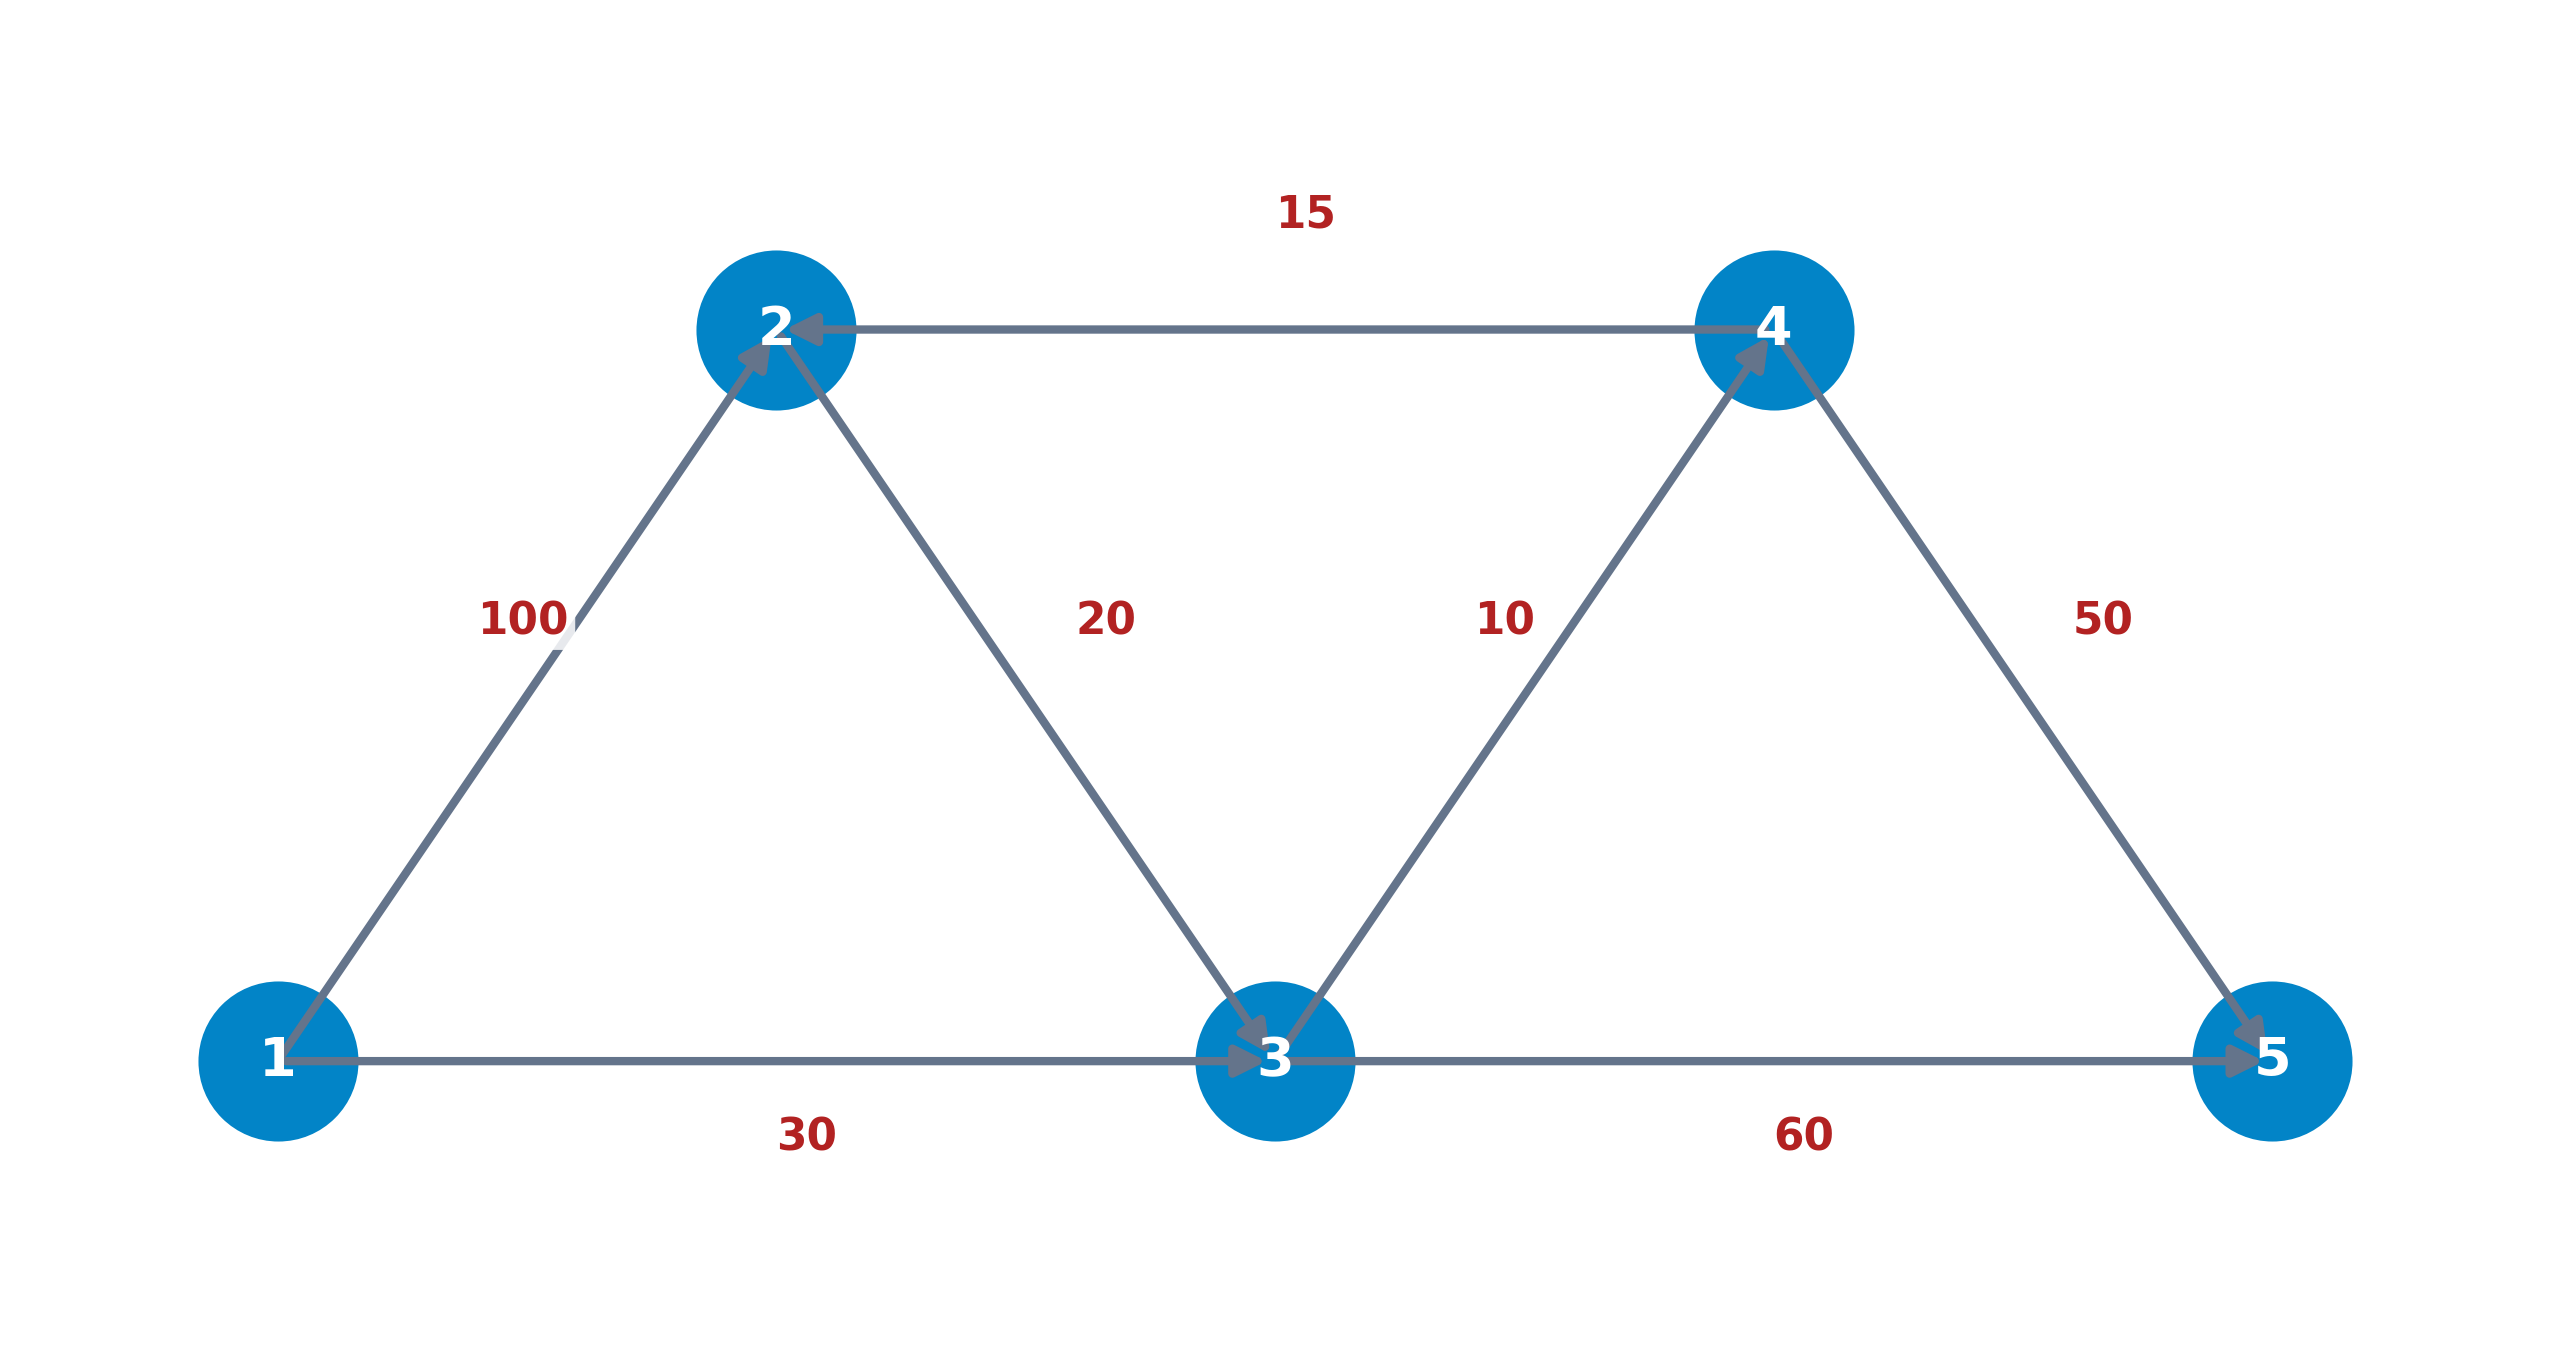
\includegraphics[width=0.7\linewidth,height=\textheight,keepaspectratio]{images/dijkstra_ejemplo_5nodos.png}

}

\caption{\label{fig-dijkstra-ejemplo-5nodos}Red dirigida valorada de 5
nodos para el ejemplo del Algoritmo de Dijkstra}

\end{figure}%

\textbf{Paso 0 (Inicialización)}:

Fijamos el nodo origen \(1\) en el conjunto de permanentes
\(\mathcal{P}\) y asignamos el vector de etiquetas iniciales \(u_j\):

\[
\begin{aligned}
u_1 &= 0 \\
u_2 &= 100 \\
u_3 &= 30 \\
u_4 &= \infty \\
u_5 &= \infty \\
\mathcal{P} &= \{1\}, \quad \mathcal{T} = \{2, 3, 4, 5\} \\
\text{Pred}(j) &= 1, \quad \forall j = 2, 3, 4, 5
\end{aligned}
\]

\textbf{Iteración 1}:

\begin{itemize}
\item
  \textbf{Selección voraz}: Identificamos el nodo transitorio con
  etiqueta provisional mínima: \[
  u_k = \min \{ u_j : j \in \mathcal{T} \} = u_3 = 30 \implies \mathcal{P} = \{1, 3\}, \quad \mathcal{T} = \{2, 4, 5\}
  \]
\item
  \textbf{Relajación de etiquetas transitorias}: Actualizamos la cota
  provisional de los nodos en \(\mathcal{T}\): \[
  \begin{aligned}
  u_2 &= \min \{ u_2, u_3 + d_{32} \} = \min \{ 100, 30 + \infty \} = 100, \quad \text{Pred}(2) = 1 \\
  u_4 &= \min \{ u_4, u_3 + d_{34} \} = \min \{ \infty, 30 + 10 \} = 40, \quad \text{Pred}(4) = 3 \\
  u_5 &= \min \{ u_5, u_3 + d_{35} \} = \min \{ \infty, 30 + 60 \} = 90, \quad \text{Pred}(5) = 3
  \end{aligned}
  \]
\end{itemize}

\textbf{Iteración 2}:

\begin{itemize}
\item
  \textbf{Selección voraz}: El nodo transitorio con etiqueta mínima en
  \(\mathcal{T} = \{2, 4, 5\}\) es: \[
  u_k = \min \{ u_j : j \in \mathcal{T} \} = u_4 = 40 \implies \mathcal{P} = \{1, 3, 4\}, \quad \mathcal{T} = \{2, 5\}
  \]
\item
  \textbf{Relajación de etiquetas transitorias}: Actualizamos la cota
  provisional para los nodos restantes en \(\mathcal{T}\): \[
  \begin{aligned}
  u_2 &= \min \{ u_2, u_4 + d_{42} \} = \min \{ 100, 40 + 15 \} = 55, \quad \text{Pred}(2) = 4 \\
  u_5 &= \min \{ u_5, u_4 + d_{45} \} = \min \{ 90, 40 + 50 \} = 90, \quad \text{Pred}(5) = 4
  \end{aligned}
  \]
\end{itemize}

\textbf{Iteración 3}:

\begin{itemize}
\item
  \textbf{Selección voraz}: El nodo transitorio con etiqueta mínima en
  \(\mathcal{T} = \{2, 5\}\) es: \[
  u_k = \min \{ u_j : j \in \mathcal{T} \} = u_2 = 55 \implies \mathcal{P} = \{1, 3, 4, 2\}, \quad \mathcal{T} = \{5\}
  \]
\item
  \textbf{Relajación de etiquetas transitorias}: \[
  u_5 = \min \{ u_5, u_2 + d_{25} \} = \min \{ 90, 55 + \infty \} = 90, \quad \text{Pred}(5) = 4
  \]
\end{itemize}

\textbf{Iteración 4}:

\begin{itemize}
\item
  \textbf{Selección voraz}: Se selecciona el último nodo transitorio: \[
  u_k = \min \{ u_j : j \in \mathcal{T} \} = u_5 = 90 \implies \mathcal{P} = \{1, 3, 4, 2, 5\}, \quad \mathcal{T} = \emptyset
  \]
\item
  \textbf{Criterio de Parada}: Al ser \(\mathcal{T} = \emptyset\), se
  detiene el procedimiento.
\end{itemize}

Al finalizar el procedimiento iterativo, se obtienen las distancias
geodésicas y los predecesores óptimos:

\begin{itemize}
\tightlist
\item
  \textbf{Vector de distancias mínimas}:
  \(\mathbf{u} = (u_1, u_2, u_3, u_4, u_5) = (0, 55, 30, 40, 90)\).
\item
  \textbf{Vector de predecesores}: \(\text{Pred} = (1, 4, 1, 3, 4)\).
\item
  \textbf{Arborescencia de caminos mínimos}: Comprendida por los arcos
  dirigidos \(\{ (1,3), (3,4), (4,2), (4,5) \}\).
\end{itemize}

\begin{figure}[H]

\centering{

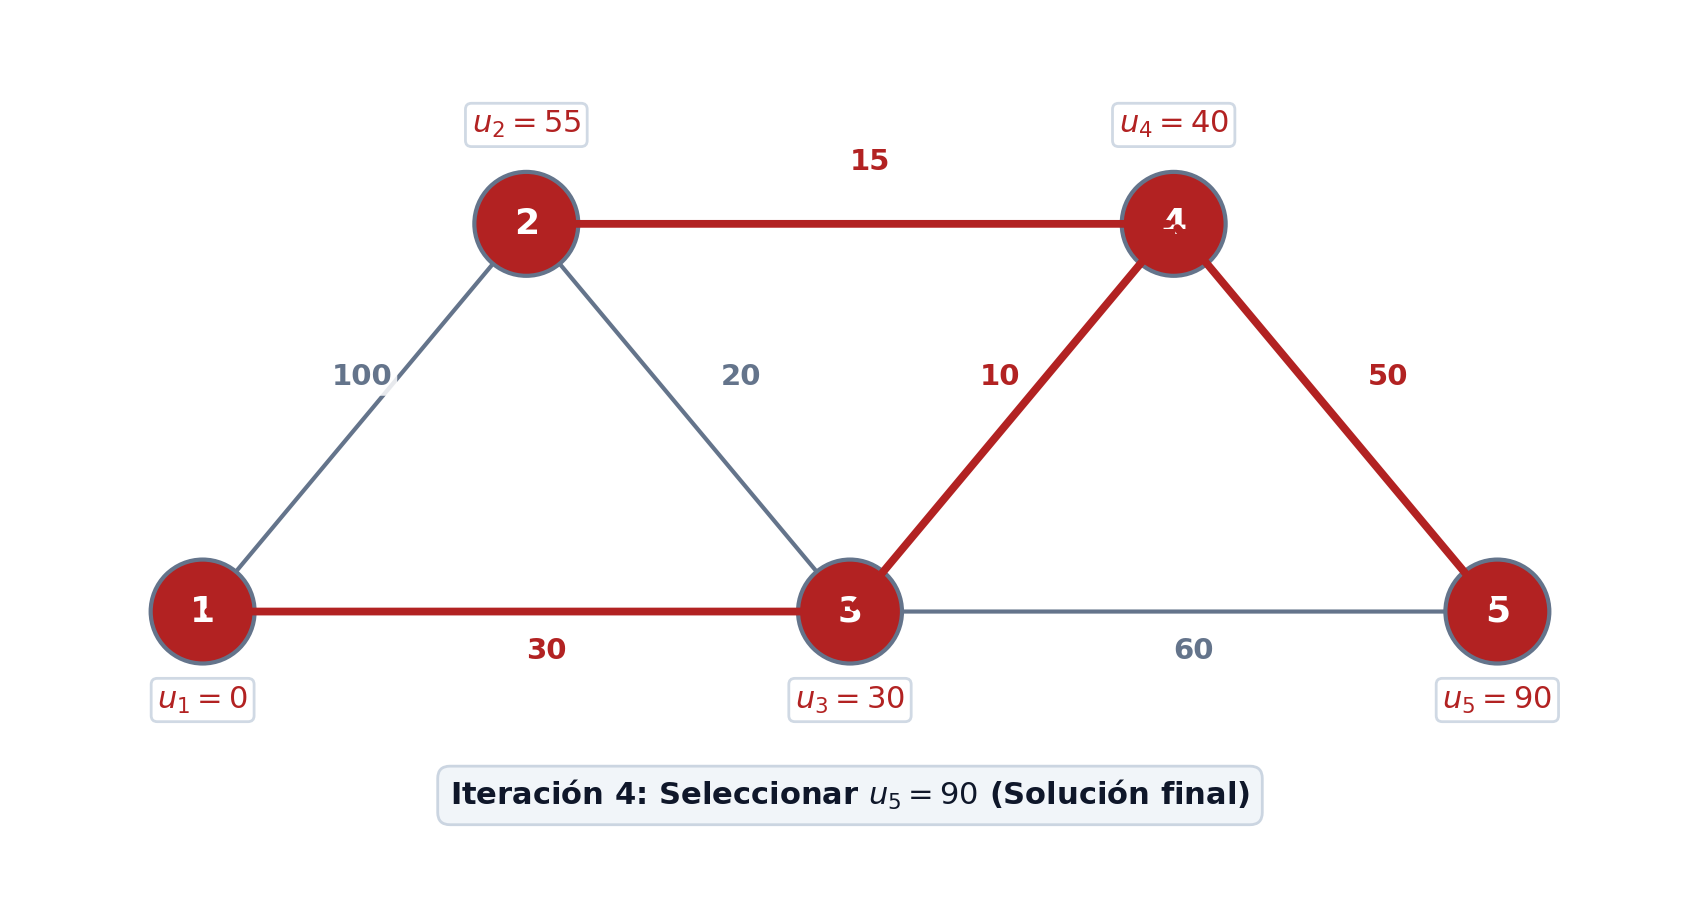
\includegraphics[width=0.75\linewidth,height=\textheight,keepaspectratio]{images/dijkstra_traza_paso_a_paso.png}

}

\caption{\label{fig-dijkstra-ejemplo-pasos}Traza gráfica de la evolución
iterativa del Algoritmo de Dijkstra paso a paso}

\end{figure}%

\end{tcolorbox}

\begin{center}\rule{0.5\linewidth}{0.5pt}\end{center}

\section{Redes con pesos negativos: Algoritmo de
Bellman-Ford}\label{redes-con-pesos-negativos-algoritmo-de-bellman-ford}

Cuando una red contiene arcos con costes negativos (\(d_{ij} < 0\)), el
algoritmo de Dijkstra pierde validez puesto que una cota provisional o
fija podría abaratarse posteriormente mediante un camino derivado de una
arista negativa. En el caso general, cuando existen arcos de longitud
negativa pero se garantiza la ausencia de circuitos de coste negativo,
una alternativa para obtener la solución de las ecuaciones de
optimalidad consiste en aproximar el camino mínimo a cualquier vértice
por la distancia del camino óptimo que utiliza \(1, 2, \dots, m\) arcos.

Esta es la idea fundamental del \textbf{Algoritmo de Bellman-Ford},
publicado por Lester R. Ford Jr.~en 1956 (Ford 1956), aunque fue
propuesto originalmente por Alfonso Shimbel en 1955 (Shimbel 1955) y
desarrollado posteriormente por Richard Bellman en 1958 (Bellman 1958) y
Edward F. Moore en 1959. Posee una complejidad algorítmica de \(O(n^3)\)
u \(O(|V| \cdot |U|)\), superior a la del algoritmo de Dijkstra.

\begin{tcolorbox}[enhanced jigsaw, toprule=.15mm, opacitybacktitle=0.6, coltitle=black, colbacktitle=quarto-callout-note-color!10!white, title=\textcolor{quarto-callout-note-color}{\faInfo}\hspace{0.5em}{Definición: Aproximación por número de arcos \(u_j^m\)}, arc=.35mm, rightrule=.15mm, toptitle=1mm, breakable, bottomtitle=1mm, titlerule=0mm, colback=white, opacityback=0, leftrule=.75mm, colframe=quarto-callout-note-color-frame, left=2mm, bottomrule=.15mm]

Sea \(u_j^m\) la longitud del camino mínimo desde el nodo origen \(1\)
al nodo \(j\) \textbf{utilizando \(m\) arcos dirigidos o menos}:

\[
u_j^m \equiv \text{longitud del camino mínimo de } 1 \text{ a } j \text{ utilizando } m \text{ arcos o menos}
\]

El procedimiento se inicia fijando \(m = 1\) e incrementa iterativamente
\(m\) hasta un máximo de \(m = n - 1\). Si la red no contiene circuitos
de longitud negativa, el algoritmo converge a la solución óptima global
en \(n - 1\) iteraciones a lo sumo, satisfaciendo la relación de
recurrencia:

\[
u_j^m = \min \left\{ u_j^{m-1}, \ \min_{k \neq j} \{ u_k^{m-1} + d_{kj} \} \right\}, \quad \forall j = 2, \dots, n
\]

\end{tcolorbox}

El desarrollo formal del procedimiento se sintetiza a través del
siguiente esquema algorítmico.

\begin{tcolorbox}[enhanced jigsaw, toprule=.15mm, opacitybacktitle=0.6, coltitle=black, colbacktitle=quarto-callout-note-color!10!white, title=\textcolor{quarto-callout-note-color}{\faInfo}\hspace{0.5em}{Esquema: Algoritmo de Bellman-Ford}, arc=.35mm, rightrule=.15mm, toptitle=1mm, breakable, bottomtitle=1mm, titlerule=0mm, colback=white, opacityback=0, leftrule=.75mm, colframe=quarto-callout-note-color-frame, left=2mm, bottomrule=.15mm]

Dada una red valorada \(G = (V, U, \mathbf{d})\) con \(n = |V|\)
vértices:

\begin{enumerate}
\def\labelenumi{\arabic{enumi}.}
\tightlist
\item
  \textbf{Paso 1 (Inicialización)}:

  \begin{itemize}
  \tightlist
  \item
    Para \(m = 1\), definir las etiquetas iniciales del camino directo:
    \[
    u_j^1 = \begin{cases} 
    0 & \text{si } j = 1 \\ 
    d_{1j} & \text{si } (1, j) \in U \\ 
    \infty & \text{si } (1, j) \notin U 
    \end{cases}
    \]
  \item
    Hacer \(m \leftarrow 1\).
  \end{itemize}
\item
  \textbf{Paso 2 (Iteración de relajación)}:

  \begin{itemize}
  \tightlist
  \item
    Hacer \(m \leftarrow m + 1\).
  \item
    Para cada nodo \(j = 2, \dots, n\), evaluar si es más ventajoso
    mantener la cota anterior o acceder a \(j\) pasando por un nodo
    intermedio \(k\): \[
    u_j^m = \min \left\{ u_j^{m-1}, \ \min_{k \neq j} \{ u_k^{m-1} + d_{kj} \} \right\}
    \]
  \end{itemize}
\item
  \textbf{Paso 3 (Criterio de Parada y Convergencia)}:

  \begin{itemize}
  \tightlist
  \item
    \textbf{Criterio de Parada Anticipada}: Si \(u_j^m = u_j^{m-1}\)
    para todo \(j = 2, \dots, n\), la solución con \(m\) arcos es óptima
    y se detiene el proceso.
  \item
    \textbf{Criterio Límite}: Si \(m = n - 1\), detener el
    procedimiento. En otro caso, regresar al Paso 2.
  \end{itemize}
\end{enumerate}

\end{tcolorbox}

\begin{tcolorbox}[enhanced jigsaw, toprule=.15mm, opacitybacktitle=0.6, coltitle=black, colbacktitle=quarto-callout-important-color!10!white, title=\textcolor{quarto-callout-important-color}{\faExclamation}\hspace{0.5em}{Teorema: Detección de circuitos de coste negativo}, arc=.35mm, rightrule=.15mm, toptitle=1mm, breakable, bottomtitle=1mm, titlerule=0mm, colback=white, opacityback=0, leftrule=.75mm, colframe=quarto-callout-important-color-frame, left=2mm, bottomrule=.15mm]

Un digrafo \(G = (V, U, \mathbf{d})\) contiene al menos un
\textbf{circuito de coste negativo} accesible desde el origen \(1\) si y
sólo si en la iteración \(m = n\) del Algoritmo de Bellman-Ford existe
al menos un nodo \(j \in V\) tal que:

\[
u_j^n \neq u_j^{n-1} \quad (\text{equivalentemente } u_j^n < u_j^{n-1})
\]

\emph{Demostración}: Cualquier camino simple en un grafo de \(n\)
vértices contiene a lo sumo \(n - 1\) arcos. Si la distancia mínima
desde el origen a un nodo \(j\) disminuye al permitir caminos de \(n\)
arcos (\(u_j^n < u_j^{n-1}\)), por el principio del palomar
(\emph{pigeonhole principle}) la ruta de \(n\) arcos debe contener
obligatoriamente un ciclo repetido. Como la distancia se ha reducido
estrictamente, dicho ciclo posee un coste total estrictamente negativo.

\end{tcolorbox}

\begin{tcolorbox}[enhanced jigsaw, toprule=.15mm, opacitybacktitle=0.6, coltitle=black, colbacktitle=quarto-callout-tip-color!10!white, title=\textcolor{quarto-callout-tip-color}{\faLightbulb}\hspace{0.5em}{Ejemplo: Aplicación del algoritmo de Bellman-Ford con costes negativos}, arc=.35mm, rightrule=.15mm, toptitle=1mm, breakable, bottomtitle=1mm, titlerule=0mm, colback=white, opacityback=0, leftrule=.75mm, colframe=quarto-callout-tip-color-frame, left=2mm, bottomrule=.15mm]

Consideremos el digrafo de 4 nodos mostrado en la
Figura~\ref{fig-bellman-ford-ejemplo-4nodos}, el cual contiene el arco
de coste negativo \((4, 2)\) con \(d_{42} = -3\). Deseamos encontrar el
camino mínimo desde el nodo \(1\) a todos los demás vértices.

\begin{figure}[H]

\centering{

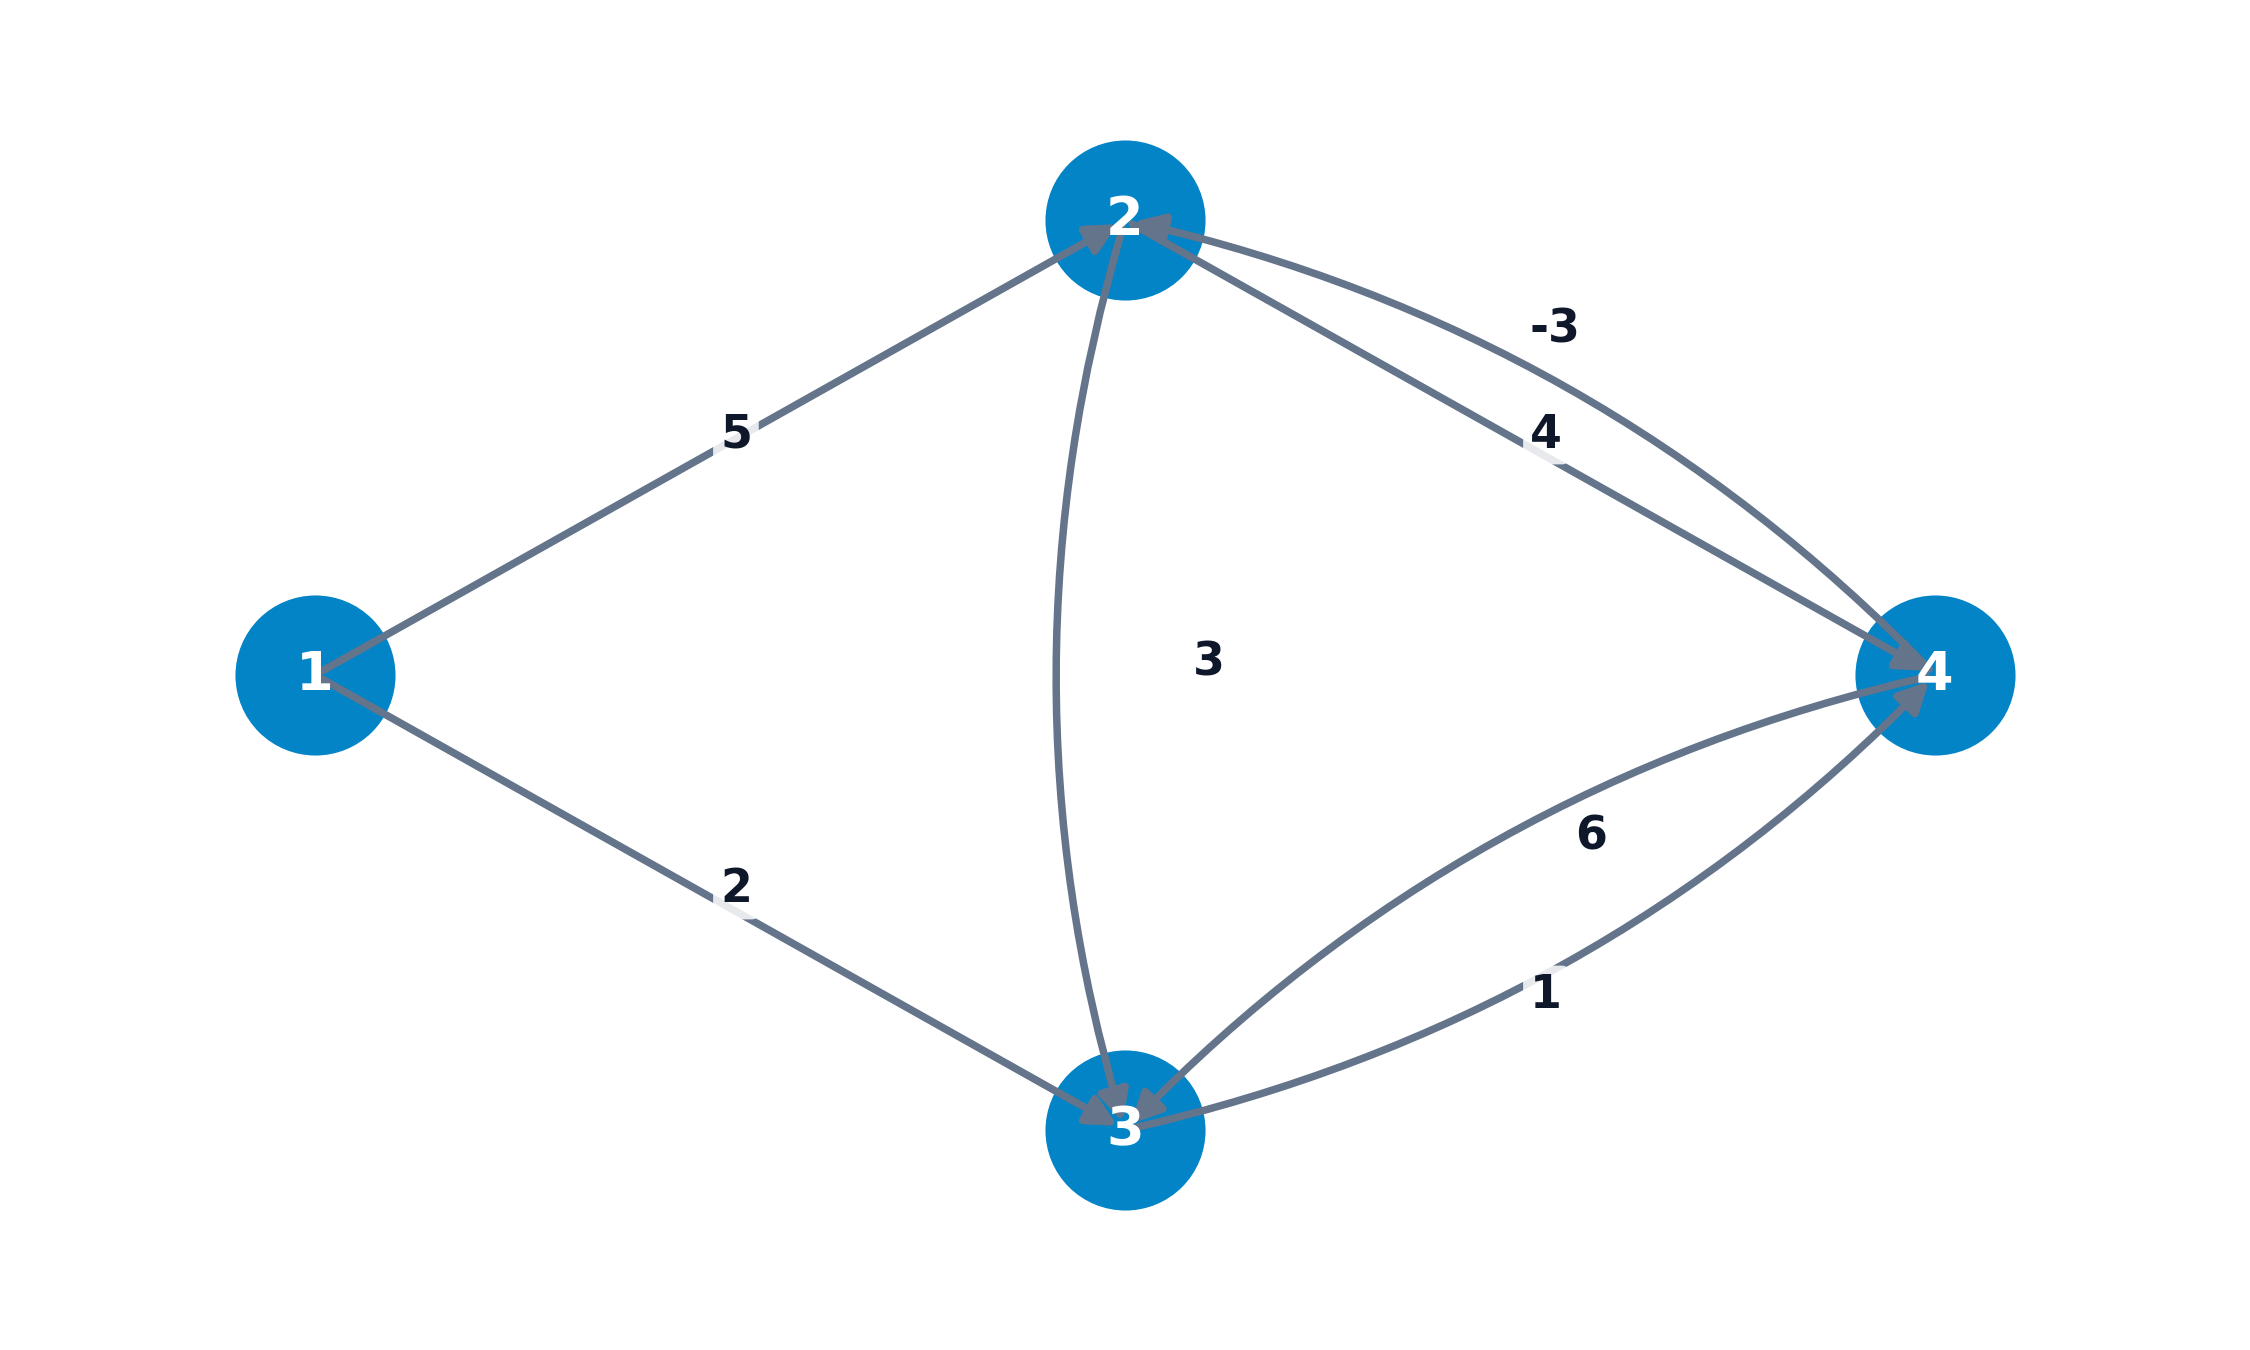
\includegraphics[width=0.65\linewidth,height=\textheight,keepaspectratio]{images/bellman_ford_ejemplo_4nodos.png}

}

\caption{\label{fig-bellman-ford-ejemplo-4nodos}Digrafo valorado de 4
nodos con costes negativos para el Algoritmo de Bellman-Ford}

\end{figure}%

\textbf{Resolución paso a paso}:

\begin{itemize}
\item
  \textbf{Paso 1 (Inicialización \(m=1\))}: \[
  \begin{aligned}
  u_1^1 &= 0 \\
  u_2^1 &= 5 \\
  u_3^1 &= 2 \\
  u_4^1 &= \infty \\
  m &= 1
  \end{aligned}
  \]
\item
  \textbf{Iteración \(m=2\)}: \[
  \begin{aligned}
  u_2^2 &= \min \{ u_2^1, \min \{ u_3^1 + d_{32}, u_4^1 + d_{42} \} \} = \min \{ 5, \min \{ 2 + \infty, \infty - 3 \} \} = 5 = u_2^1 \\
  u_3^2 &= \min \{ u_3^1, \min \{ u_2^1 + d_{23}, u_4^1 + d_{43} \} \} = \min \{ 2, \min \{ 5 + 3, \infty + 6 \} \} = 2 = u_3^1 \\
  u_4^2 &= \min \{ u_4^1, \min \{ u_2^1 + d_{24}, u_3^1 + d_{34} \} \} = \min \{ \infty, \min \{ 5 + 4, 2 + 1 \} \} = 3 \neq u_4^1 \\
  m &= 2
  \end{aligned}
  \]
\item
  \textbf{Iteración \(m=3\)}: \[
  \begin{aligned}
  u_2^3 &= \min \{ u_2^2, \min \{ u_3^2 + d_{32}, u_4^2 + d_{42} \} \} = \min \{ 5, \min \{ 2 + \infty, 3 - 3 \} \} = 0 \neq u_2^2 \\
  u_3^3 &= \min \{ u_3^2, \min \{ u_2^2 + d_{23}, u_4^2 + d_{43} \} \} = \min \{ 2, \min \{ 5 + 3, 3 + 6 \} \} = 2 = u_3^2 \\
  u_4^3 &= \min \{ u_4^2, \min \{ u_2^2 + d_{24}, u_3^2 + d_{34} \} \} = \min \{ 3, \min \{ 5 + 4, 2 + 1 \} \} = 3 = u_4^2 \\
  m &= 3
  \end{aligned}
  \]
\item
  \textbf{Iteración \(m=4\)}: \[
  \begin{aligned}
  u_2^4 &= \min \{ u_2^3, \min \{ u_3^3 + d_{32}, u_4^3 + d_{42} \} \} = \min \{ 0, \min \{ 2 + \infty, 3 - 3 \} \} = 0 = u_2^3 \\
  u_3^4 &= \min \{ u_3^3, \min \{ u_2^3 + d_{23}, u_4^3 + d_{43} \} \} = \min \{ 2, \min \{ 0 + 3, 3 + 6 \} \} = 2 = u_3^3 \\
  u_4^4 &= \min \{ u_4^3, \min \{ u_2^3 + d_{24}, u_3^3 + d_{34} \} \} = \min \{ 3, \min \{ 0 + 4, 2 + 1 \} \} = 3 = u_4^2 \\
  m &= 4
  \end{aligned}
  \]
\end{itemize}

Como \(u^4 = u^3 = (0, 0, 2, 3)\), se alcanza la \textbf{convergencia y
parada anticipada}.

Al finalizar el procedimiento iterativo, se obtienen las distancias
geodésicas y los predecesores óptimos:

\begin{itemize}
\tightlist
\item
  \textbf{Vector de distancias mínimas}:
  \(\mathbf{u} = (u_1, u_2, u_3, u_4) = (0, 0, 2, 3)\).
\item
  \textbf{Vector de predecesores}: \(\text{Pred} = (1, 4, 1, 3)\).
\item
  \textbf{Arborescencia de caminos mínimos}: Comprendida por los arcos
  dirigidos \(\{ (1,3), (3,4), (4,2) \}\).
\end{itemize}

\begin{figure}[H]

\centering{

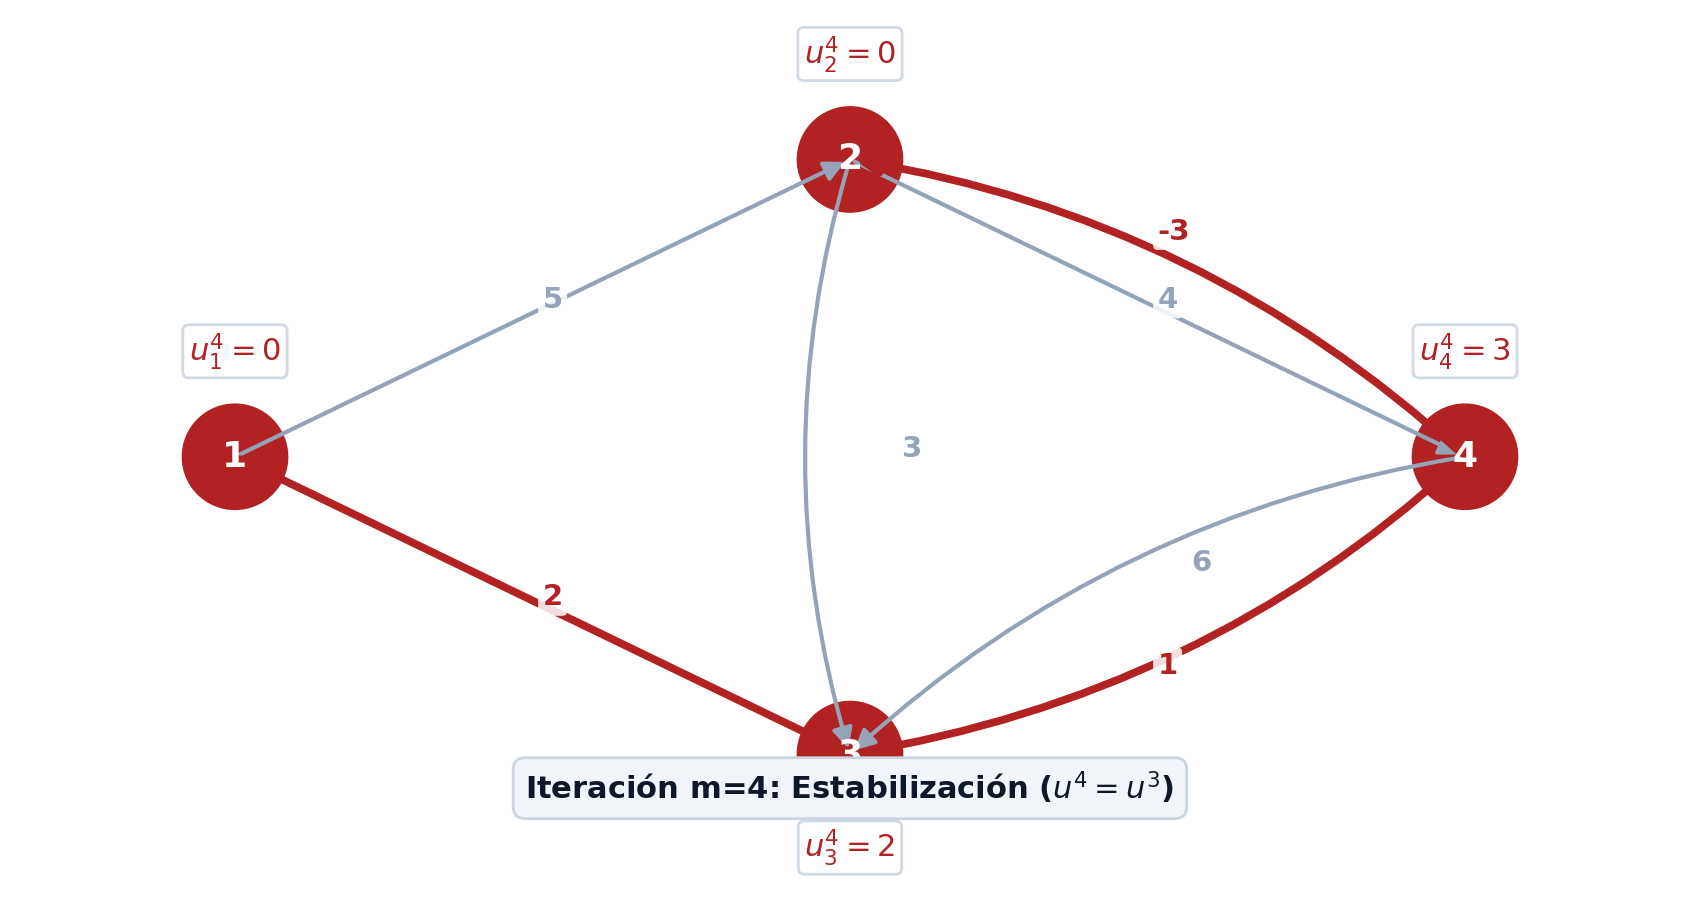
\includegraphics[width=0.75\linewidth,height=\textheight,keepaspectratio]{images/bellman_ford_traza_paso_a_paso.png}

}

\caption{\label{fig-bellman-ford-ejemplo-pasos}Traza gráfica de la
evolución iterativa del Algoritmo de Bellman-Ford paso a paso}

\end{figure}%

\end{tcolorbox}

En el análisis de redes valoradas, una de las mayores utilidades del
algoritmo de Bellman-Ford radica en su capacidad para detectar la
presencia de \textbf{circuitos de coste o longitud negativa}. Si un
digrafo contiene un circuito con suma de pesos estrictamente negativa,
la longitud del camino óptimo hacia los nodos que componen dicho
circuito o accesibles desde él tiende hacia \(-\infty\), requiriendo un
número infinito de arcos para su recorrido.

Por el contrario, cuando la red carece de circuitos negativos, la
distancia mínima hacia cualquier vértice accesible se alcanza utilizando
como máximo \(n - 1\) arcos. Esta propiedad permite adaptar el algoritmo
para realizar una iteración suplementaria hasta \(m = n\):

\begin{itemize}
\tightlist
\item
  Si el digrafo \textbf{no contiene circuitos de longitud negativa}, las
  etiquetas de la pasada \(n - 1\) y de la pasada \(n\) resultarán ser
  estrictamente idénticas (\(u^{n-1} = u^n\)).
\item
  Si alguna etiqueta \(u_j^m = \infty\), no existe ningún camino físico
  de conexión desde el origen \(1\) hacia el nodo \(j\).
\item
  Si en la iteración \(m = n\) se detecta que
  \textbf{\(u^{n-1} \neq u^n\)} (con \(u_j^n < u_j^{n-1}\) para algún
  nodo \(j\)), queda demostrada formalmente la existencia de un
  \textbf{circuito de longitud negativa} en la red.
\end{itemize}

\begin{tcolorbox}[enhanced jigsaw, toprule=.15mm, opacitybacktitle=0.6, coltitle=black, colbacktitle=quarto-callout-note-color!10!white, title=\textcolor{quarto-callout-note-color}{\faInfo}\hspace{0.5em}{Esquema: Algoritmo de Bellman-Ford adaptado para detección de circuitos
negativos}, arc=.35mm, rightrule=.15mm, toptitle=1mm, breakable, bottomtitle=1mm, titlerule=0mm, colback=white, opacityback=0, leftrule=.75mm, colframe=quarto-callout-note-color-frame, left=2mm, bottomrule=.15mm]

Dada una red valorada general \(G = (V, U, \mathbf{d})\) con \(n = |V|\)
vértices:

\begin{enumerate}
\def\labelenumi{\arabic{enumi}.}
\tightlist
\item
  \textbf{Paso 1 (Inicialización)}:

  \begin{itemize}
  \tightlist
  \item
    Asignar las etiquetas iniciales para \(m = 1\): \[
    u_j^1 = \begin{cases} 
    0 & \text{si } j = 1 \\ 
    d_{1j} & \text{si } (1, j) \in U \\ 
    \infty & \text{si } (1, j) \notin U 
    \end{cases}
    \]
  \item
    Hacer \(m \leftarrow 1\).
  \end{itemize}
\item
  \textbf{Paso 2 (Relajación iterativa)}:

  \begin{itemize}
  \tightlist
  \item
    Hacer \(m \leftarrow m + 1\).
  \item
    Para cada nodo \(j = 2, \dots, n\), evaluar: \[
    u_j^m = \min \left\{ u_j^{m-1}, \ \min_{k \neq j} \{ u_k^{m-1} + d_{kj} \} \right\}
    \]
  \end{itemize}
\item
  \textbf{Paso 3 (Evaluación de optimalidad o detección de circuito)}:

  \begin{itemize}
  \tightlist
  \item
    \textbf{Criterio de Convergencia Óptima}: Si \(u_j^m = u_j^{m-1}\)
    para todo \(j = 2, \dots, n\), detener el algoritmo: la solución
    actual \(u^m\) es óptima.
  \item
    \textbf{Criterio de Detección de Circuito Negativo}: En otro caso,
    si \(m = n\), detener el procedimiento concluyendo que
    \textbf{existen circuitos de longitud negativa} en la red.
  \item
    En otro caso (\(m < n\)), regresar al Paso 2.
  \end{itemize}
\end{enumerate}

\end{tcolorbox}

\begin{tcolorbox}[enhanced jigsaw, toprule=.15mm, opacitybacktitle=0.6, coltitle=black, colbacktitle=quarto-callout-tip-color!10!white, title=\textcolor{quarto-callout-tip-color}{\faLightbulb}\hspace{0.5em}{Ejemplo: Detección de un circuito de longitud negativa en un digrafo de
7 nodos}, arc=.35mm, rightrule=.15mm, toptitle=1mm, breakable, bottomtitle=1mm, titlerule=0mm, colback=white, opacityback=0, leftrule=.75mm, colframe=quarto-callout-tip-color-frame, left=2mm, bottomrule=.15mm]

Consideremos el digrafo de 7 nodos (\(V = \{a, b, c, d, e, f, g\}\) con
\(n = 7\)) representado en la
Figura~\ref{fig-bellman-ford-circuito-negativo-7nodos}, con origen en el
nodo \(a\).

\begin{figure}[H]

\centering{

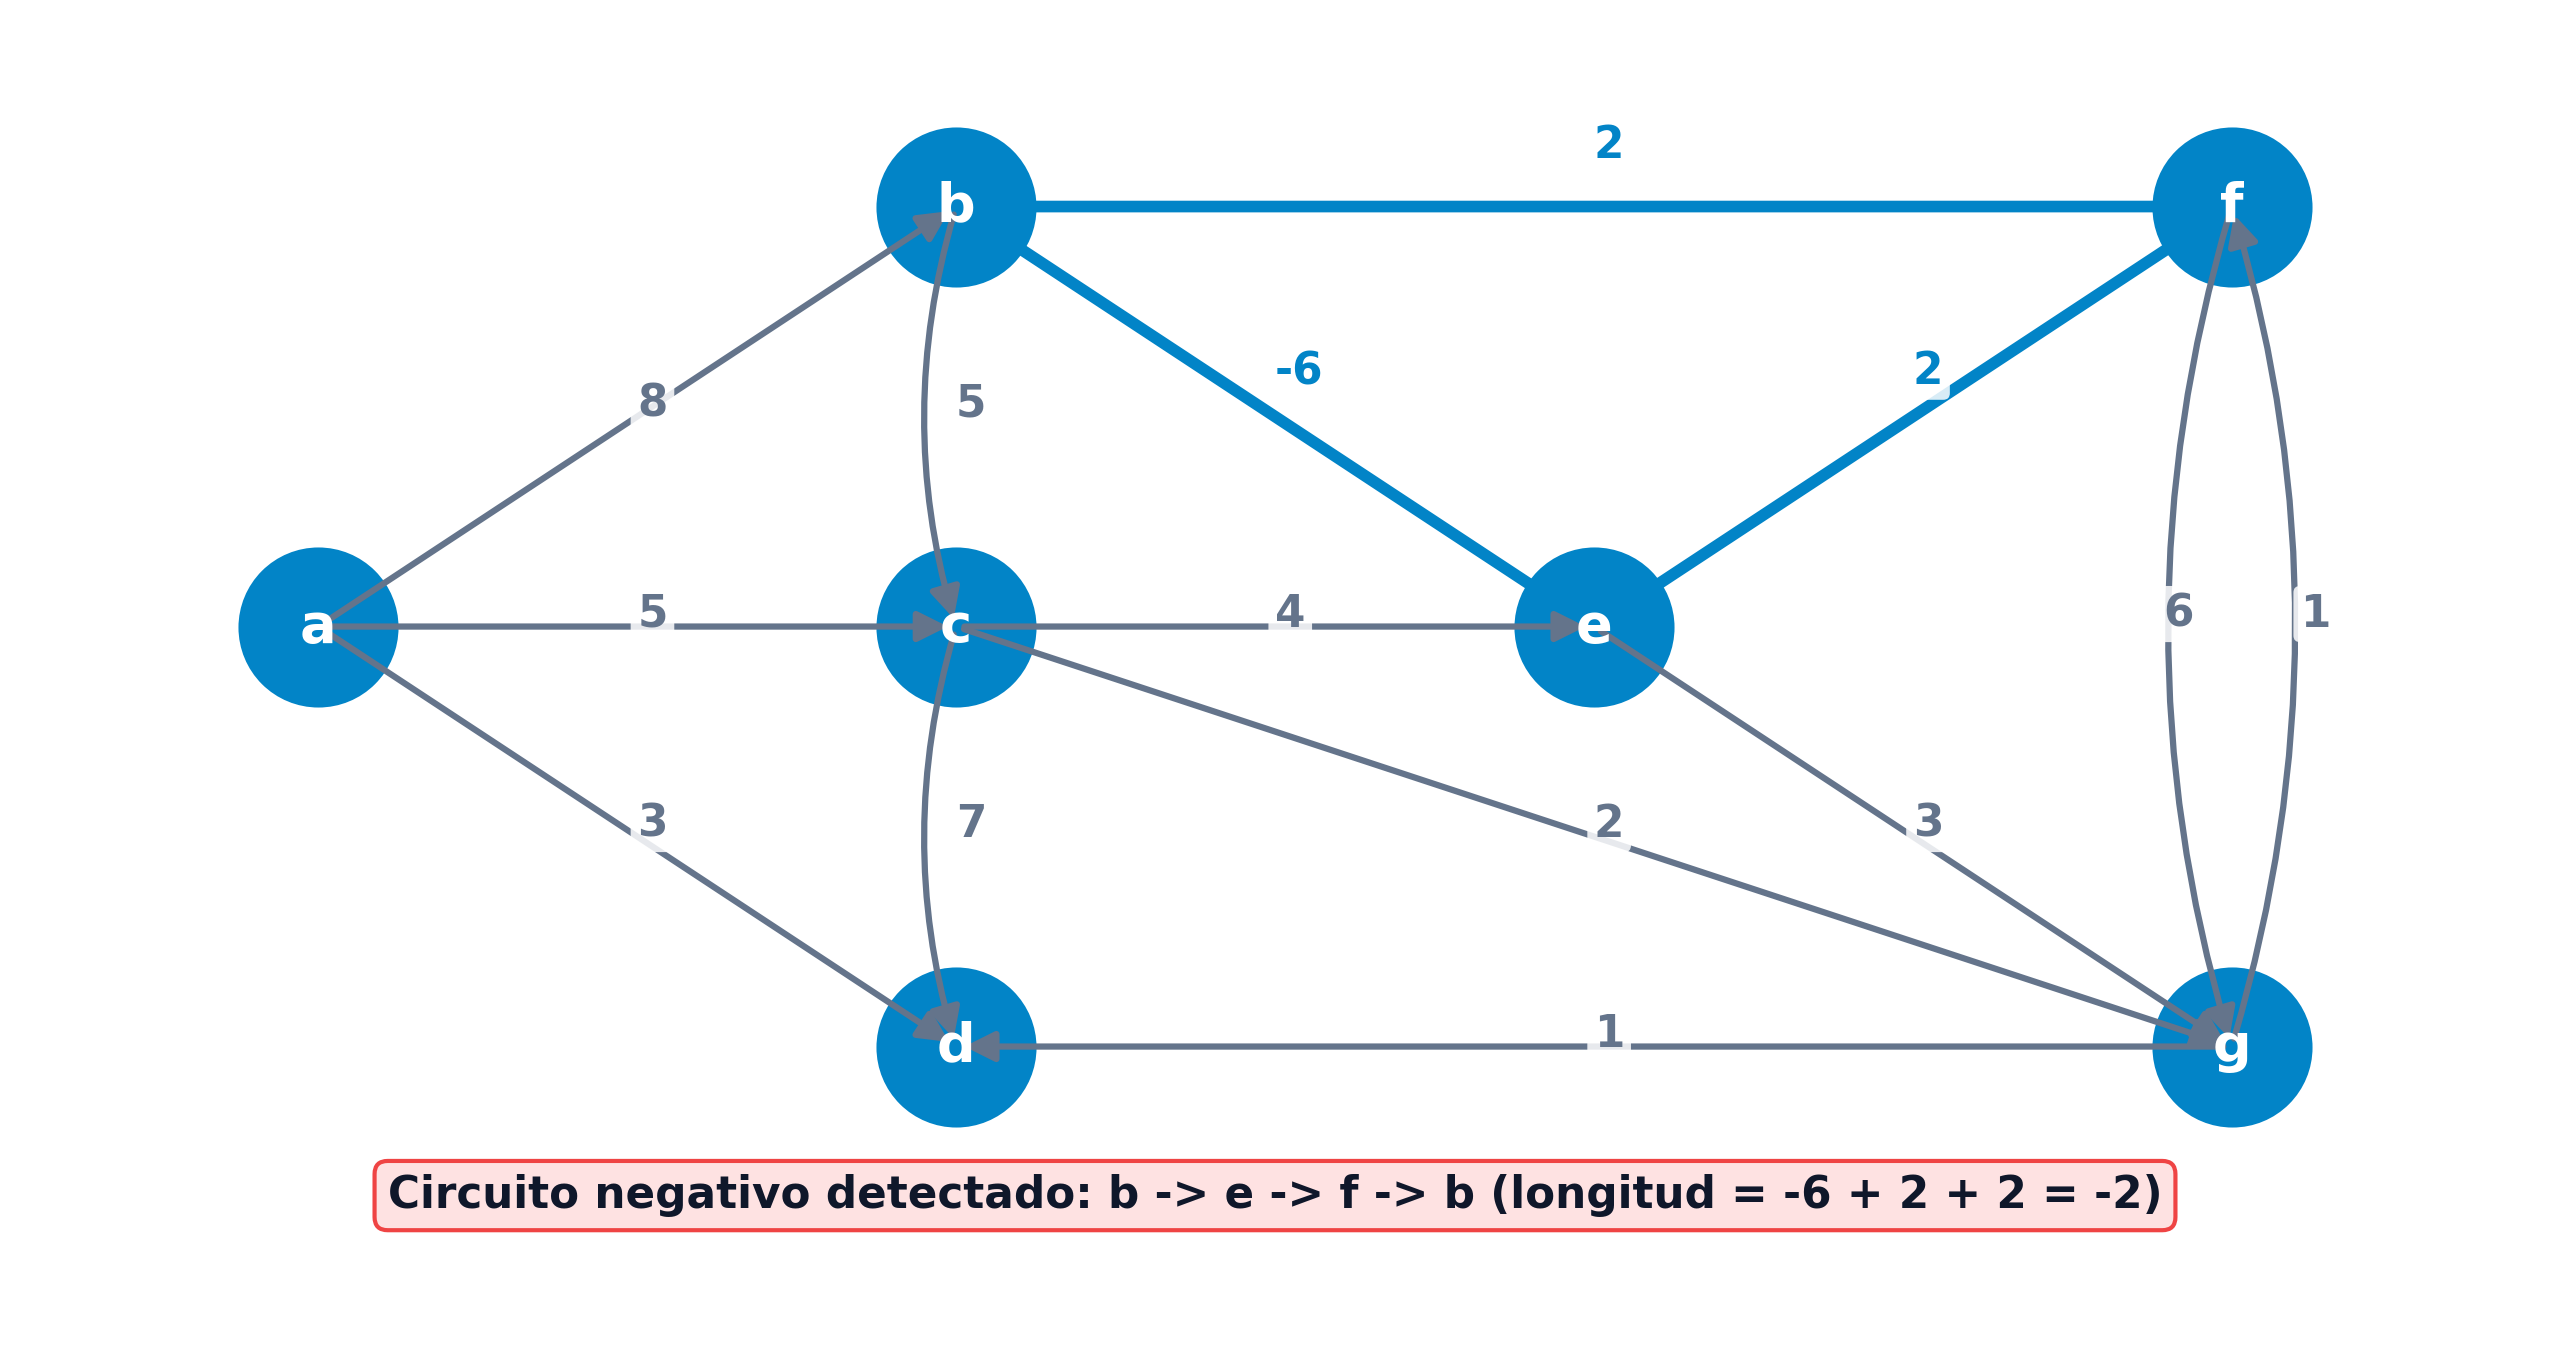
\includegraphics[width=0.75\linewidth,height=\textheight,keepaspectratio]{images/bellman_ford_circuito_negativo_7nodos.png}

}

\caption{\label{fig-bellman-ford-circuito-negativo-7nodos}Digrafo
valorado de 7 nodos con un circuito de longitud negativa}

\end{figure}%

Inspeccionando los ciclos de la red, observamos que la secuencia
\(b \to e \to f \to b\) conforma un circuito cerrado de longitud
acumulada negativa:

\[
d(b, e) + d(e, f) + d(f, b) = -6 + 2 + 2 = -2 < 0
\]

\textbf{Desarrollo del Algoritmo de Bellman-Ford}:

\begin{itemize}
\item
  \textbf{Paso 1 (Inicialización \(m=1\))}: \[
  u_a^1 = 0, \quad u_b^1 = 8, \quad u_c^1 = 5, \quad u_d^1 = 3, \quad u_e^1 = \infty, \quad u_f^1 = \infty, \quad u_g^1 = \infty
  \]
\item
  \textbf{Tras ejecutar el procedimiento hasta la iteración
  \(m = n - 1 = 6\)}, se obtiene el vector de etiquetas: \[
  u_a^6 = 0, \quad u_b^6 = 6, \quad u_c^6 = 5, \quad u_d^6 = 3, \quad u_e^6 = 0, \quad u_f^6 = 2, \quad u_g^6 = 3
  \]
\item
  \textbf{Iteración suplementaria \(m = n = 7\)}: Evaluamos la
  relajación de etiquetas para todos los nodos del digrafo: \[
  \begin{aligned}
  u_b^7 &= \min \{ u_b^6, u_a^6 + 8, u_f^6 + 2 \} = \min \{ 6, 0 + 8, 2 + 2 \} = 4 \\
  u_c^7 &= \min \{ u_c^6, u_a^6 + 5, u_b^6 + 5 \} = \min \{ 5, 0 + 5, 4 + 5 \} = 5 \\
  u_d^7 &= \min \{ u_d^6, u_a^6 + 3, u_c^6 + 7, u_g^6 + 1 \} = \min \{ 3, 0 + 3, 5 + 7, 3 + 1 \} = 3 \\
  u_e^7 &= \min \{ u_e^6, u_b^6 - 6, u_c^6 + 4 \} = \min \{ 0, 6 - 6, 5 + 4 \} = 0 \\
  u_f^7 &= \min \{ u_f^6, u_e^6 + 2, u_g^6 + 6 \} = \min \{ 2, 0 + 2, 3 + 6 \} = 2 \\
  u_g^7 &= \min \{ u_g^6, u_c^6 + 2, u_e^6 + 3, u_f^6 + 1 \} = \min \{ 3, 5 + 2, 0 + 3, 2 + 1 \} = 3
  \end{aligned}
  \]
\end{itemize}

Al comparar las etiquetas entre las iteraciones 6 y 7, detectamos que
para el nodo \(b\):

\[
u_b^6 = 6 \neq 4 = u_b^7 \implies u_b^7 < u_b^6
\]

Puesto que \(u^7 \neq u^6\), el algoritmo se detiene formalmente en
\(m = n = 7\) concluyendo que \textbf{existe un circuito de longitud
negativa} (\(b \to e \to f \to b\)).

\end{tcolorbox}

\begin{center}\rule{0.5\linewidth}{0.5pt}\end{center}

\section{Formulación matemática: Programación Lineal Primal y
Dual}\label{formulaciuxf3n-matemuxe1tica-programaciuxf3n-lineal-primal-y-dual}

El problema del camino mínimo entre un nodo origen \(s\) y un nodo
destino \(t\) en un digrafo valorado \(G = (V, U, \mathbf{d})\) admite
una representación equivalente mediante un \textbf{modelo de
programación lineal}. Desde la perspectiva de la teoría de redes de
flujo, el problema equivale a transportar una unidad de flujo unitario
desde el nodo fuente \(s\) hasta el nodo sumidero \(t\) con el menor
coste o distancia acumulada posible.

\begin{tcolorbox}[enhanced jigsaw, toprule=.15mm, opacitybacktitle=0.6, coltitle=black, colbacktitle=quarto-callout-note-color!10!white, title=\textcolor{quarto-callout-note-color}{\faInfo}\hspace{0.5em}{Definición: Modelo Primal de Programación Lineal para el Camino Mínimo}, arc=.35mm, rightrule=.15mm, toptitle=1mm, breakable, bottomtitle=1mm, titlerule=0mm, colback=white, opacityback=0, leftrule=.75mm, colframe=quarto-callout-note-color-frame, left=2mm, bottomrule=.15mm]

Dada una red dirigida \(G = (V, U, \mathbf{d})\) con \(n = |V|\)
vértices, etiquetados de forma que \(s \in V\) representa el origen y
\(t \in V\) el destino, asociamos a cada arco \((i, j) \in U\) un coste
unitario de transporte dado por su peso \(d_{ij}\).

Definimos las \textbf{variables de decisión} \(x_{ij}\) como variables
indicadoras de flujo que determinan la activación de cada arco en el
itinerario:

\[
x_{ij} = \begin{cases} 
1 & \text{si el arco } (i, j) \text{ forma parte del camino mínimo} \\ 
0 & \text{en otro caso} 
\end{cases} \quad \forall (i, j) \in U
\]

El modelo lineal minimiza la longitud total del trayecto sujeto a las
ecuaciones de balance y conservación de flujo en cada vértice de la red:

\[
\begin{aligned}
\min_{\mathbf{x}} \quad & \sum_{i=1}^n \sum_{j=1}^n d_{ij} x_{ij} \\
\text{sujeto a} \quad & \sum_{k=1}^n x_{sk} = 1 \quad (\text{Salida unitaria del nodo origen } s) \\
& \sum_{k=1}^n x_{kt} = 1 \quad (\text{Entrada unitaria al nodo destino } t) \\
& \sum_{j=1}^n x_{jk} = \sum_{i=1}^n x_{ki}, \quad \forall k \neq s, t \quad (\text{Conservación de flujo en nodos intermedios}) \\
& x_{ij} \in \{0, 1\}, \quad \forall (i, j) \in U
\end{aligned}
\]

\end{tcolorbox}

En notación matricial compacta, el modelo se expresa como
\(\min \{ \mathbf{d}^T \mathbf{x} : \mathbf{A} \mathbf{x} = \mathbf{b}, \, \mathbf{x} \ge \mathbf{0} \}\),
donde \(\mathbf{A} \in \{-1, 0, 1\}^{n \times m}\) representa la
\textbf{matriz de incidencia nodo-arco} del digrafo y
\(\mathbf{b} = (1, 0, \dots, 0, -1)^T\) es el vector de balances
nodales.

\begin{tcolorbox}[enhanced jigsaw, toprule=.15mm, opacitybacktitle=0.6, coltitle=black, colbacktitle=quarto-callout-important-color!10!white, title=\textcolor{quarto-callout-important-color}{\faExclamation}\hspace{0.5em}{Teorema: Total unimodularidad e integridad del modelo primal}, arc=.35mm, rightrule=.15mm, toptitle=1mm, breakable, bottomtitle=1mm, titlerule=0mm, colback=white, opacityback=0, leftrule=.75mm, colframe=quarto-callout-important-color-frame, left=2mm, bottomrule=.15mm]

La matriz de incidencia nodo-arco \(\mathbf{A}\) de cualquier grafo o
digrafo es \textbf{totalmente unimodular} (TUM). Por consiguiente, para
cualquier vector de balances entero \(\mathbf{b}\), todas las soluciones
básicas factibles del problema de programación lineal continuo son
\textbf{estrictamente enteras}.

En particular, la solución óptima del modelo continuo satisface
automáticamente \(x_{ij}^* \in \{0, 1\}\), seleccionando una ruta simple
óptima de \(s\) a \(t\) sin necesidad de imponer de forma explícita
restricciones de programación entera.

\end{tcolorbox}

A partir de la formulación primal, se puede derivar el \textbf{modelo
dual} asociando a la ecuación de balance de cada nodo \(i \in V\) una
variable dual no restringida en signo \(u_i \in \mathbb{R}\), denominada
\textbf{potencial nodal}:

\[
\begin{aligned}
\max_{\mathbf{u}} \quad & u_t - u_s \\
\text{sujeto a} \quad & u_j - u_i \le d_{ij}, \quad \forall (i, j) \in U \\
& u_i \text{ no restringidas}, \quad \forall i \in V
\end{aligned}
\]

\begin{tcolorbox}[enhanced jigsaw, toprule=.15mm, opacitybacktitle=0.6, coltitle=black, colbacktitle=quarto-callout-note-color!10!white, title=\textcolor{quarto-callout-note-color}{\faInfo}\hspace{0.5em}{Interpretación física y económica del modelo dual}, arc=.35mm, rightrule=.15mm, toptitle=1mm, breakable, bottomtitle=1mm, titlerule=0mm, colback=white, opacityback=0, leftrule=.75mm, colframe=quarto-callout-note-color-frame, left=2mm, bottomrule=.15mm]

\begin{itemize}
\tightlist
\item
  \textbf{Potenciales Nodales}: Las variables duales \(u_i\) representan
  \textbf{potenciales o tensiones nodales} en la red.
\item
  \textbf{Fijación de Referencia}: Dado que el sistema dual presenta un
  grado de libertad adicional (es invariante ante sumas constantes
  \(u_i + C\)), al fijar el origen \(u_s = 0\), la variable dual óptima
  \(u_j^*\) coincide exactamente con la \textbf{distancia mínima
  \(d(s, j)\)} desde \(s\) hasta \(j\).
\item
  \textbf{Restricción de Consistencia}: La condición
  \(u_j - u_i \le d_{ij}\) establece que la diferencia de potencial
  entre dos nodos adyacentes no puede superar la distancia directa del
  arco que los une.
\item
  \textbf{Holgura Complementaria}: Si el arco \((i, j)\) forma parte del
  camino mínimo óptimo (\(x_{ij}^* = 1\)), la restricción dual
  correspondiente se activa con igualdad estricta:
  \(u_j^* - u_i^* = d_{ij}\).
\end{itemize}

\end{tcolorbox}

\begin{tcolorbox}[enhanced jigsaw, toprule=.15mm, opacitybacktitle=0.6, coltitle=black, colbacktitle=quarto-callout-tip-color!10!white, title=\textcolor{quarto-callout-tip-color}{\faLightbulb}\hspace{0.5em}{Ejemplo: Formulación primal completa para una red de 7 nodos}, arc=.35mm, rightrule=.15mm, toptitle=1mm, breakable, bottomtitle=1mm, titlerule=0mm, colback=white, opacityback=0, leftrule=.75mm, colframe=quarto-callout-tip-color-frame, left=2mm, bottomrule=.15mm]

Consideremos el digrafo de 7 nodos \(V = \{s, 1, 2, 3, 4, 5, t\}\)
representado en la Figura~\ref{fig-linear-programming-ejemplo-7nodos}.
Se desea formular el modelo de programación lineal para resolver el
problema del camino mínimo entre el nodo origen \(s\) y el nodo destino
\(t\).

\begin{figure}[H]

\centering{

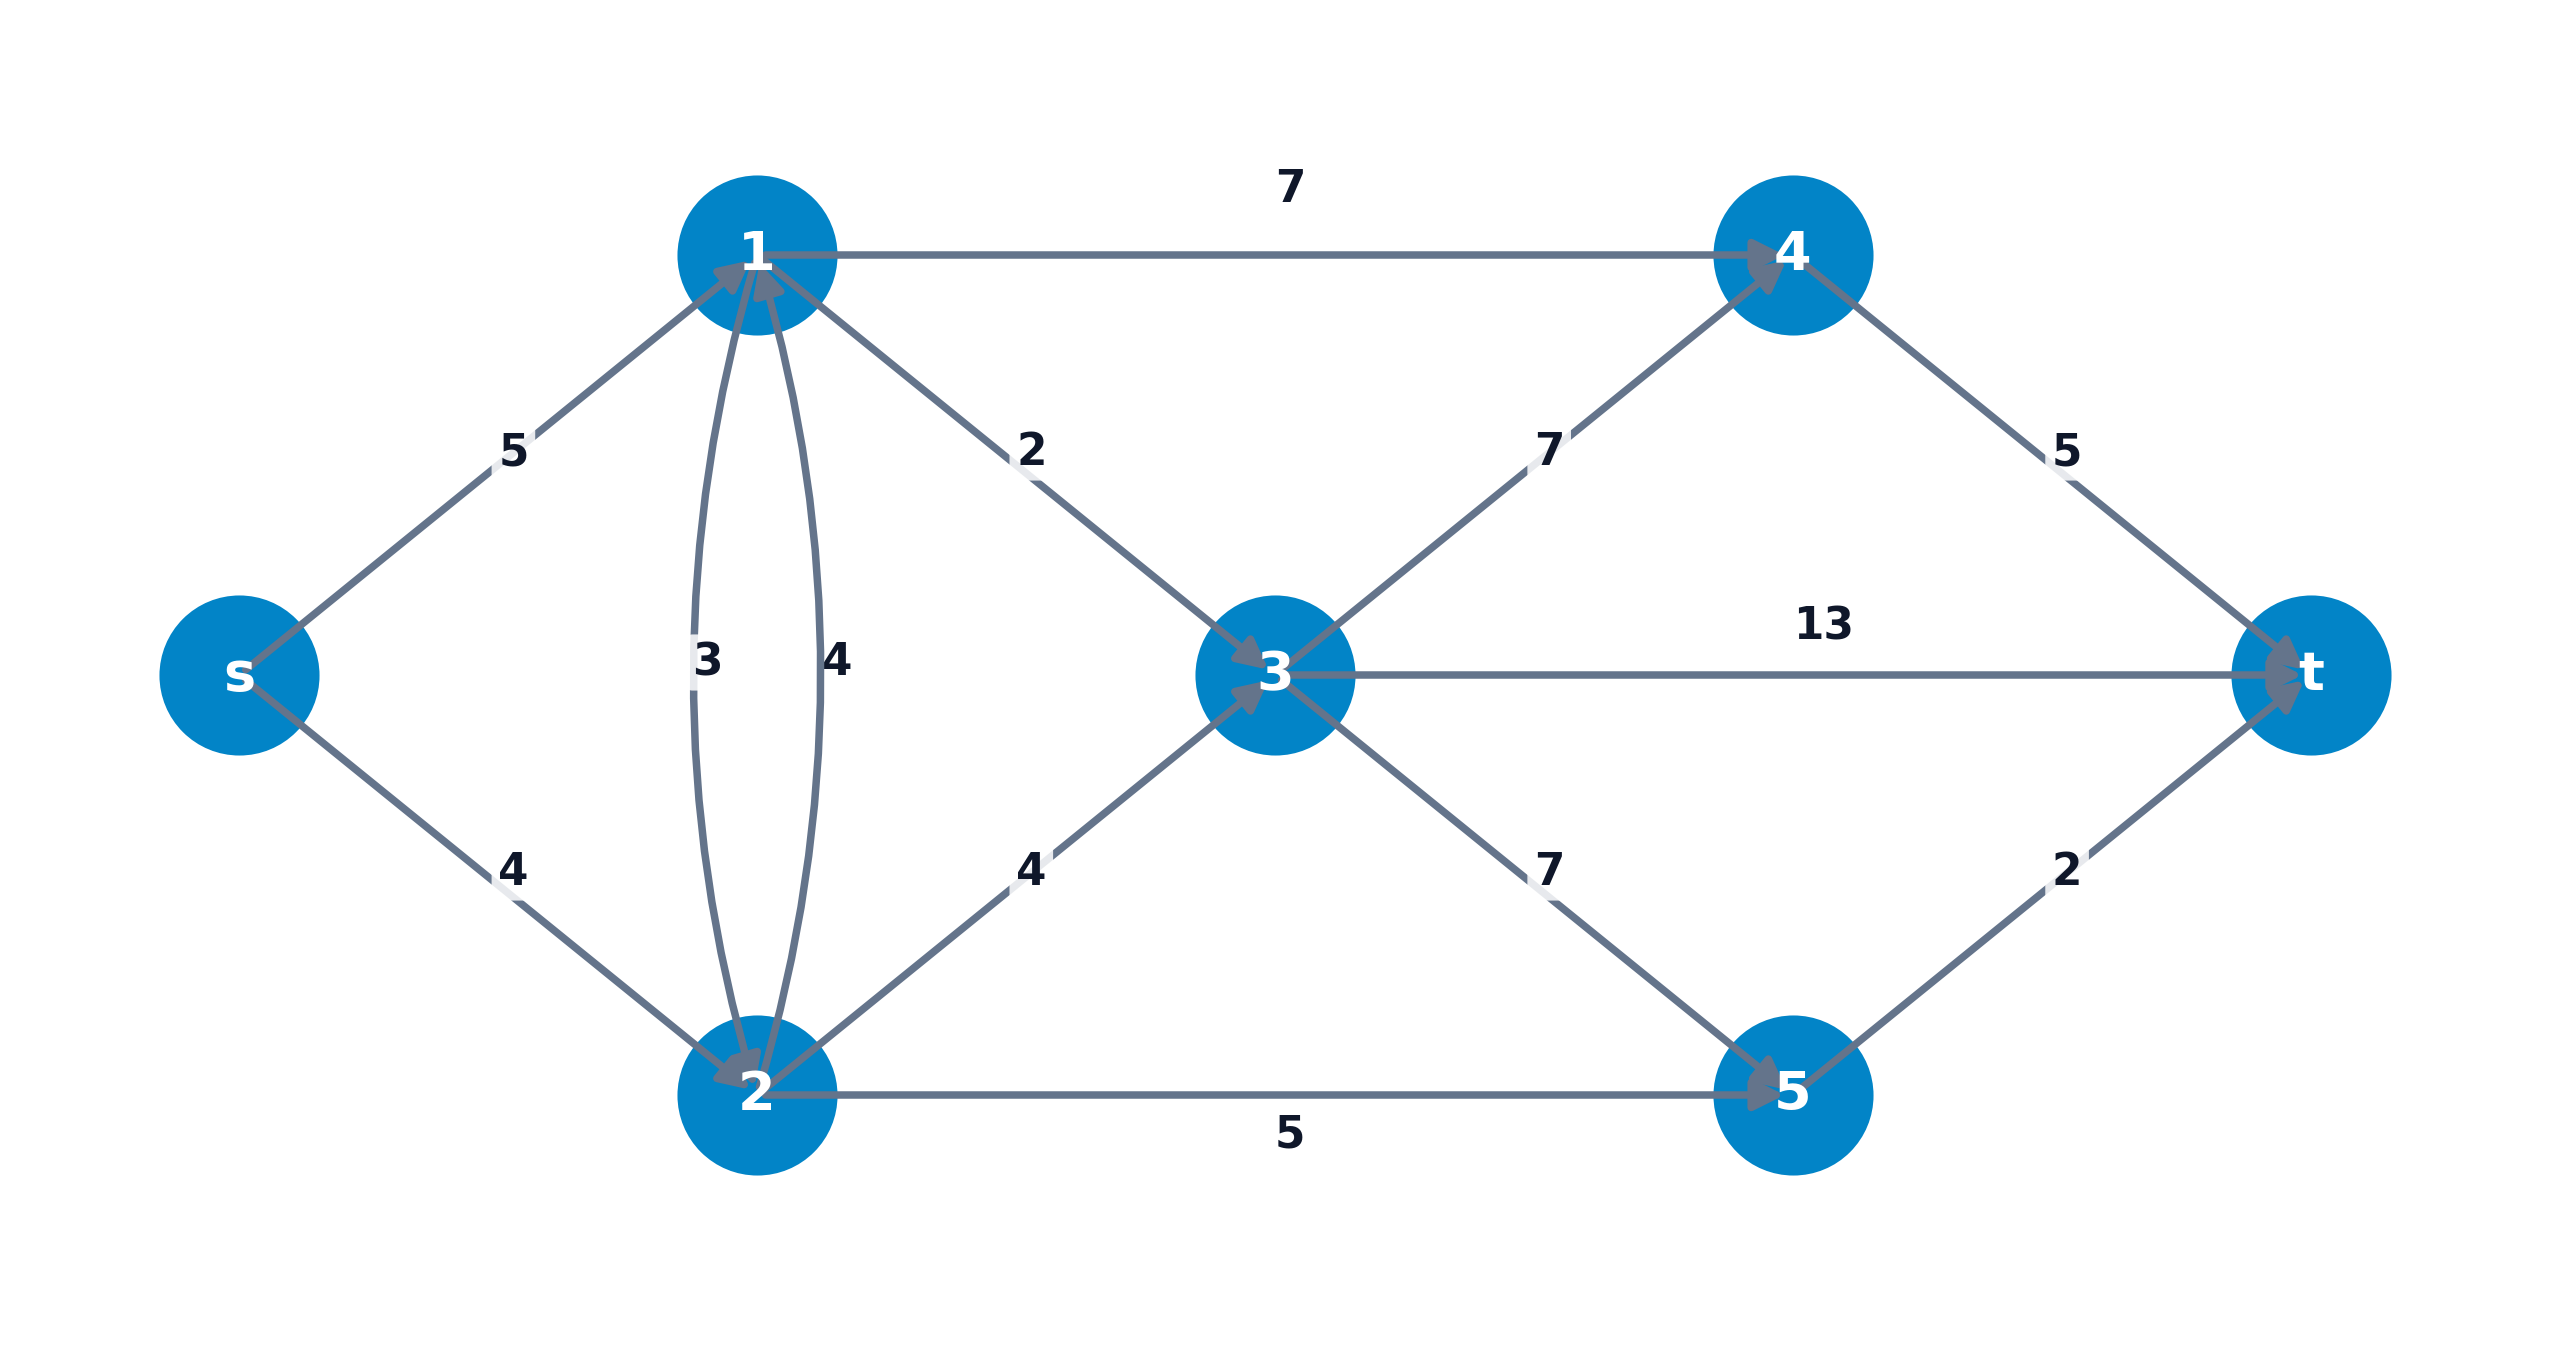
\includegraphics[width=0.75\linewidth,height=\textheight,keepaspectratio]{images/linear_programming_ejemplo_7nodos.png}

}

\caption{\label{fig-linear-programming-ejemplo-7nodos}Digrafo valorado
de 7 nodos para el modelo de programación lineal del camino mínimo}

\end{figure}%

\textbf{1. Variables de decisión}: \[
x_{ij} = \begin{cases} 
1 & \text{si el arco } (i, j) \text{ forma parte del camino} \\ 
0 & \text{en otro caso} 
\end{cases} \quad \forall (i, j) \in U
\]

\textbf{2. Función objetivo}: Minimizar la suma de costes de los arcos
seleccionados en el itinerario: \[
\begin{aligned}
\min z = \ & 5 x_{s1} + 4 x_{s2} + 4 x_{12} + 2 x_{13} + 7 x_{14} + 3 x_{21} + 4 x_{23} \\
& + 5 x_{25} + 7 x_{34} + 7 x_{35} + 13 x_{3t} + 5 x_{4t} + 2 x_{5t}
\end{aligned}
\]

\textbf{3. Restricciones del nodo origen (\(s\))}: Garantizar la salida
de una unidad de flujo desde el origen: \[
x_{s1} + x_{s2} = 1
\]

\textbf{4. Restricciones del nodo destino (\(t\))}: Garantizar la
llegada de una unidad de flujo al destino: \[
x_{3t} + x_{4t} + x_{5t} = 1
\]

\textbf{5. Restricciones de conservación de flujo en el resto de nodos
(\(k \neq s, t\))}: La suma de flujos entrantes a un nodo debe ser igual
a la suma de flujos salientes: \[
\begin{aligned}
\text{Nodo 1:} \quad & x_{s1} + x_{21} = x_{12} + x_{13} + x_{14} \\
\text{Nodo 2:} \quad & x_{s2} + x_{12} = x_{21} + x_{23} + x_{25} \\
\text{Nodo 3:} \quad & x_{13} + x_{23} = x_{34} + x_{35} + x_{3t} \\
\text{Nodo 4:} \quad & x_{14} + x_{34} = x_{4t} \\
\text{Nodo 5:} \quad & x_{25} + x_{35} = x_{5t}
\end{aligned}
\]

\textbf{6. Naturaleza de las variables}: \[
x_{ij} \in \{0, 1\}, \quad \forall (i, j) \in U
\]

\end{tcolorbox}

\begin{center}\rule{0.5\linewidth}{0.5pt}\end{center}

\section{Caminos mínimos entre todos los pares de
nodos}\label{caminos-muxednimos-entre-todos-los-pares-de-nodos}

En diversas aplicaciones prácticas de diseño de redes de comunicación,
logística e infraestructura, se requiere determinar las distancias
mínimas entre \textbf{todos los pares de vértices
\((i, j) \in V \times V\)}.

Una primera aproximación intuitiva consiste en ejecutar \(n\) veces un
algoritmo de origen único (como Dijkstra o Bellman-Ford), tomando
secuencialmente cada vértice \(i \in V\) como raíz del cálculo. Sin
embargo, en digrafos con pesos negativos, aplicar \(n\) veces el
algoritmo de Bellman-Ford multiplica la complejidad computacional por
\(n\), alcanzando una cota total de \(n \times O(n^3) = O(n^4)\). Este
enfoque resulta ineficiente al desaprovechar la estructura compartida de
los subcaminos óptimos en la red.

Para resolver de forma global este problema optimizando la reutilización
de información, exploraremos primeramente el \textbf{método basado en la
multiplicación de matrices} (álgebra Min-Suma) y, a continuación, el
\textbf{algoritmo de Floyd-Warshall} basado en programación dinámica.

\begin{center}\rule{0.5\linewidth}{0.5pt}\end{center}

\subsection{Método basado en la multiplicación de matrices (Álgebra
Min-Suma)}\label{muxe9todo-basado-en-la-multiplicaciuxf3n-de-matrices-uxe1lgebra-min-suma}

Sea \(G = (V, U, \mathbf{d})\) un digrafo valorado con \(n = |V|\)
vértices. Definimos la \textbf{matriz inicial de distancias}
\(D = (d_{kj}) \in \mathbb{R}^{n \times n}\) asociada a los arcos
directos de la red como:

\[
d_{kj} = \begin{cases} 
0 & \text{si } k = j \\ 
d_{kj} & \text{si } (k, j) \in U \\ 
\infty & \text{si } (k, j) \notin U 
\end{cases}
\]

Es posible definir un álgebra de matrices sobre la estructura de
semianillo \((\mathbb{R} \cup \{\infty\}, \min, +)\), conocida como
\textbf{álgebra Min-Suma} o \emph{álgebra tropical}, donde la operación
de suma matricial convencional se sustituye por la minimización
(\(\min\)) y la multiplicación por la adición (\(+\)).

\begin{tcolorbox}[enhanced jigsaw, toprule=.15mm, opacitybacktitle=0.6, coltitle=black, colbacktitle=quarto-callout-note-color!10!white, title=\textcolor{quarto-callout-note-color}{\faInfo}\hspace{0.5em}{Definición: Operador del producto matricial Min-Suma}, arc=.35mm, rightrule=.15mm, toptitle=1mm, breakable, bottomtitle=1mm, titlerule=0mm, colback=white, opacityback=0, leftrule=.75mm, colframe=quarto-callout-note-color-frame, left=2mm, bottomrule=.15mm]

Dadas dos matrices \(A, B \in \overline{\mathbb{R}}^{n \times n}\), el
\textbf{producto matricial Min-Suma} \(C = A \otimes B\) sustituye el
sumatorio \(\sum\) por el operador \(\min\) y el producto escalar por la
suma:

\[
\text{Álgebra Estándar: } c_{ij} = \sum_{k=1}^n a_{ik} \cdot b_{kj} \quad \implies \quad \text{Álgebra Min-Suma: } c_{ij} = \min_{1 \le k \le n} \left\{ a_{ik} + b_{kj} \right\}
\]

\begin{itemize}
\tightlist
\item
  \textbf{Paralelismo con el Algoritmo de Bellman-Ford}: La fila
  \(i\)-ésima de la matriz \(D^{(m)} = D^{(m-1)} \otimes D\) contiene
  las distancias mínimas alcanzables en a lo sumo \(m\) arcos
  considerando al nodo \(i\) como origen único.
\end{itemize}

\end{tcolorbox}

Bajo este operador, la potencia \(m\)-ésima de la matriz
\(D^m = (d_{ij})^m\) contiene la distancia mínima entre cada par de
nodos \(i\) y \(j\) utilizando \textbf{a lo sumo \(m\) arcos}. En
particular, la ordenación por filas de \(D^m\) equivale a resolver
simultáneamente una iteración del algoritmo de Bellman-Ford para los
\(n\) posibles orígenes de la red.

Para \(m = 2\), la cota de distancia de \(i\) a \(j\) utilizando 2 arcos
o menos se calcula como:

\[
(d_{ij})^2 = \min \left\{ d_{ij}, \ \min_{k \in V} \{ d_{ik} + d_{kj} \} \right\}
\]

En general, la relación de recurrencia para la potencia \((m+1)\)-ésima
adopta la forma:

\[
(d_{ij})^{m+1} = \min \left\{ (d_{ij})^m, \ \min_{k \in V} \{ (d_{ik})^m + d_{kj} \} \right\}
\]

Dado que cualquier camino simple en un grafo de \(n\) vértices contiene
a lo sumo \(n - 1\) arcos, el algoritmo alcanza la solución exacta al
calcular \(D^{n-1}\). La evaluación secuencial de
\(D, D^2, D^3, \dots, D^{n-1}\) requiere \(n - 1\) multiplicaciones de
matrices de dimensión \(n \times n\), con un coste computacional de
\(O(n^4)\).

\begin{tcolorbox}[enhanced jigsaw, toprule=.15mm, opacitybacktitle=0.6, coltitle=black, colbacktitle=quarto-callout-note-color!10!white, title=\textcolor{quarto-callout-note-color}{\faInfo}\hspace{0.5em}{Optimización por Exponenciación Binaria (Repeated Squaring)}, arc=.35mm, rightrule=.15mm, toptitle=1mm, breakable, bottomtitle=1mm, titlerule=0mm, colback=white, opacityback=0, leftrule=.75mm, colframe=quarto-callout-note-color-frame, left=2mm, bottomrule=.15mm]

Si únicamente se requiere calcular la matriz de distancias mínimas
absolutas (sin necesidad de reconstruir la secuencia explícita de
vértices del camino), es posible reducir significativamente la
complejidad algorítmica.

En lugar de evaluar secuencialmente \(D^2, D^3, \dots, D^n\), podemos
aplicar la técnica de \textbf{exponenciación binaria} calculando la
serie de potencias cuadráticas \(D^2, D^4, D^8, \dots, D^{2^k}\) hasta
superar \(n - 1\). Con esta estrategia, el número de multiplicaciones
matriciales se reduce de \(n - 1\) a \(\lceil \log_2(n - 1) \rceil\),
reduciendo la complejidad total de \(O(n^4)\) a
\textbf{\(O(n^3 \log n)\)}.

\end{tcolorbox}

\begin{tcolorbox}[enhanced jigsaw, toprule=.15mm, opacitybacktitle=0.6, coltitle=black, colbacktitle=quarto-callout-tip-color!10!white, title=\textcolor{quarto-callout-tip-color}{\faLightbulb}\hspace{0.5em}{Ejemplo: Aplicación del método de multiplicación de matrices en una red
de 4 nodos}, arc=.35mm, rightrule=.15mm, toptitle=1mm, breakable, bottomtitle=1mm, titlerule=0mm, colback=white, opacityback=0, leftrule=.75mm, colframe=quarto-callout-tip-color-frame, left=2mm, bottomrule=.15mm]

Consideremos el digrafo de 4 nodos mostrado en la
Figura~\ref{fig-matrix-multiplication-ejemplo-4nodos}, el cual contiene
arcos dirigidos con pesos positivos y negativos.

\begin{figure}[H]

\centering{

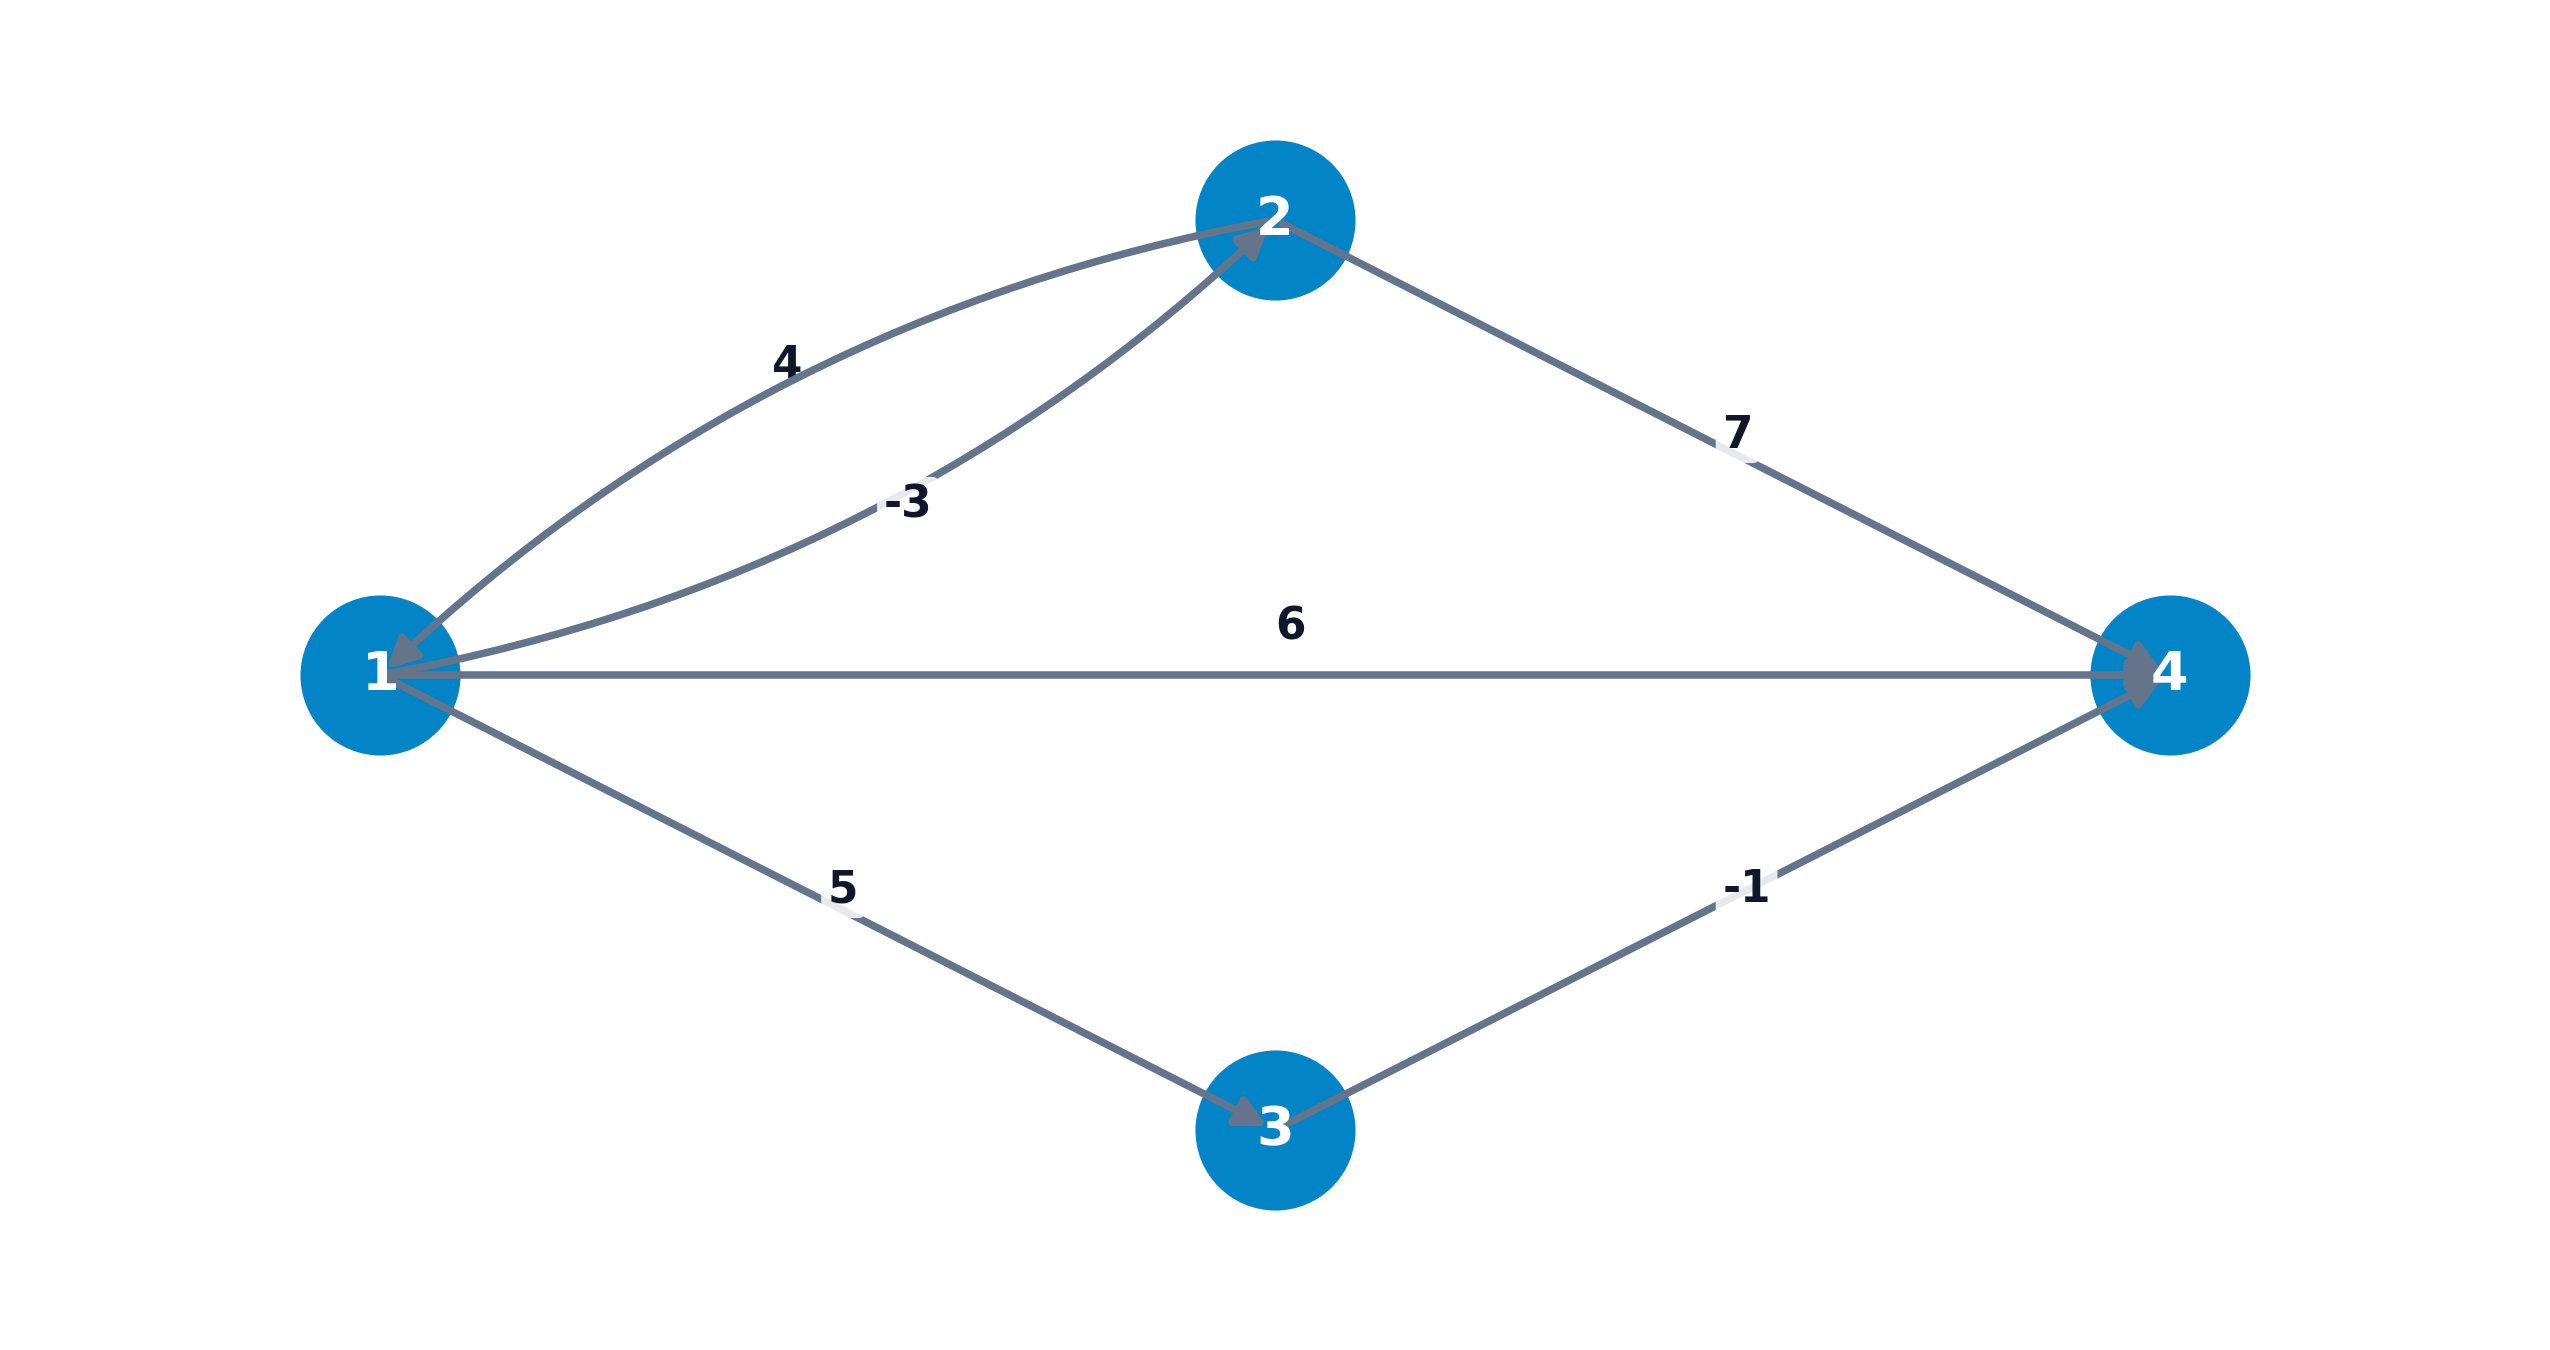
\includegraphics[width=0.65\linewidth,height=\textheight,keepaspectratio]{images/matrix_multiplication_ejemplo_4nodos.png}

}

\caption{\label{fig-matrix-multiplication-ejemplo-4nodos}Digrafo
valorado de 4 nodos para la multiplicación de matrices}

\end{figure}%

\textbf{1. Matriz inicial de distancias \(D = D^{(1)}\)}: \[
D = \begin{pmatrix}
0 & 4 & 5 & 6 \\
-3 & 0 & \infty & 7 \\
\infty & \infty & 0 & -1 \\
\infty & \infty & \infty & 0
\end{pmatrix}
\]

\textbf{2. Segunda iteración (\(D^{(2)} = D \otimes D\))}: Evaluando la
relajación con a lo sumo 2 arcos: \[
D^{(2)} = \begin{pmatrix}
0 & 4 & 5 & \textcolor{forestgreen}{\mathbf{4}} \\
-3 & 0 & \textcolor{forestgreen}{\mathbf{2}} & \textcolor{forestgreen}{\mathbf{3}} \\
\infty & \infty & 0 & -1 \\
\infty & \infty & \infty & 0
\end{pmatrix}
\] \emph{Observación}:
\((d_{14})^2 = \min \{ 6, \min \{ 0+6, 4+7, 5-1 \} \} = \min \{ 6, 5 \} = \textcolor{forestgreen}{\mathbf{4}}\)
vía el camino \(1 \to 3 \to 4\).

\textbf{3. Tercera iteración (\(D^{(3)} = D^{(2)} \otimes D\))}:
Evaluando la relajación con a lo sumo 3 arcos: \[
D^{(3)} = \begin{pmatrix}
0 & 4 & 5 & 4 \\
-3 & 0 & 2 & \textcolor{forestgreen}{\mathbf{1}} \\
\infty & \infty & 0 & -1 \\
\infty & \infty & \infty & 0
\end{pmatrix}
\] \emph{Observación}: La primera fila de \(D^{(3)}\) coincide
exactamente con el resultado obtenido al ejecutar el algoritmo de
Bellman-Ford con origen en el nodo 1.

Puesto que \(n = 4\), el algoritmo se detiene formalmente en
\(D^{(n-1)} = D^{(3)}\) o en la iteración donde la matriz de distancias
permanezca invariante (\(D^{(m)} = D^{(m-1)}\)).

\end{tcolorbox}

\begin{center}\rule{0.5\linewidth}{0.5pt}\end{center}

\subsection{Algoritmo de
Floyd-Warshall}\label{algoritmo-de-floyd-warshall}

El \textbf{Algoritmo de Floyd-Warshall} fue publicado formalmente por
Floyd en 1962 (Floyd 1962), aunque una versión equivalente del método
fue propuesta previamente por Roy en 1959 (Roy 1959) y desarrollada
posteriormente de forma independiente por Warshall en 1962 (Warshall
1962).

Se trata de un algoritmo de \textbf{programación dinámica} válido para
calcular las distancias mínimas entre cualquier par de nodos en redes
que pueden contener arcos de peso negativo (siempre que se garantice la
ausencia de circuitos de coste negativo). Su complejidad algorítmica es
\textbf{\(O(n^3)\)}, siendo significativamente más eficiente que
ejecutar \(n\) veces el algoritmo de Bellman-Ford (\(O(n^4)\)).

La idea fundamental del algoritmo consiste en iterar sobre cada nodo
intermedio candidato \(k \in \{1, \dots, n\}\), comparando para cada par
de nodos \((i, j)\) si el camino óptimo de \(i\) a \(j\) mejora al
incorporar el nodo \(k\) como vértice intermedio.

\begin{tcolorbox}[enhanced jigsaw, toprule=.15mm, opacitybacktitle=0.6, coltitle=black, colbacktitle=quarto-callout-note-color!10!white, title=\textcolor{quarto-callout-note-color}{\faInfo}\hspace{0.5em}{Definición: Recurrencia de programación dinámica de Floyd-Warshall}, arc=.35mm, rightrule=.15mm, toptitle=1mm, breakable, bottomtitle=1mm, titlerule=0mm, colback=white, opacityback=0, leftrule=.75mm, colframe=quarto-callout-note-color-frame, left=2mm, bottomrule=.15mm]

Sea \(d_{ij}^{(k)}\) la longitud del camino mínimo desde el nodo \(i\)
hasta el nodo \(j\) permitiendo utilizar como \textbf{nodos intermedios
únicamente un subconjunto de los primeros \(k\) nodos}
\(\{1, 2, \dots, k\}\).

\begin{itemize}
\tightlist
\item
  \textbf{Inicialización (\(k = 0\))}: \(d_{ij}^{(0)} = d_{ij}\)
  (distancias directas de los arcos en la matriz \(D\)).
\item
  \textbf{Paso iterativo \(k\)}: Para cada par de vértices \((i, j)\),
  se compara:

  \begin{enumerate}
  \def\labelenumi{\arabic{enumi}.}
  \tightlist
  \item
    La longitud del camino óptimo de \(i\) a \(j\) sin utilizar el nodo
    \(k\) como intermedio (\(d_{ij}^{(k-1)}\)).
  \item
    La suma de las distancias mínimas de \(i\) a \(k\) y de \(k\) a
    \(j\) utilizando únicamente los primeros \(k-1\) nodos
    (\(d_{ik}^{(k-1)} + d_{kj}^{(k-1)}\)).
  \end{enumerate}
\end{itemize}

Si la distancia total mejora al transitar por el nodo \(k\), se
actualiza el camino mínimo mediante la relación de recurrencia:

\[
d_{ij}^{(k)} = \min \left\{ d_{ij}^{(k-1)}, \ d_{ik}^{(k-1)} + d_{kj}^{(k-1)} \right\}, \quad \forall i, j \in V
\]

\end{tcolorbox}

Puesto que el algoritmo realiza \(n\) iteraciones principales (una por
cada nodo intermedio \(k\)) y en cada iteración ejecuta \(n^2\)
comparaciones escalares (una por cada par \((i, j)\)), la complejidad
temporal global queda acotada exactamente por:

\[
n \times n^2 = O(n^3)
\]

Adicionalmente, en cada iteración se puede ir registrando de forma
paralela la matriz de predecesores \(P^{(k)}\) para posibilitar la
reconstrucción explícita de los caminos mínimos.

\begin{tcolorbox}[enhanced jigsaw, toprule=.15mm, opacitybacktitle=0.6, coltitle=black, colbacktitle=quarto-callout-note-color!10!white, title=\textcolor{quarto-callout-note-color}{\faInfo}\hspace{0.5em}{Esquema: Algoritmo de Floyd-Warshall}, arc=.35mm, rightrule=.15mm, toptitle=1mm, breakable, bottomtitle=1mm, titlerule=0mm, colback=white, opacityback=0, leftrule=.75mm, colframe=quarto-callout-note-color-frame, left=2mm, bottomrule=.15mm]

Dada la matriz de distancias directas \(D^{(0)} = D\) y la matriz de
predecesores iniciales \(P^{(0)}\) con \(P_{ij} = j\) para todo
\((i, j) \in U\):

\begin{enumerate}
\def\labelenumi{\arabic{enumi}.}
\tightlist
\item
  \textbf{Bucle externo (Nodo pivote intermedio \(k\))}: Para
  \(k = 1, 2, \dots, n\):
\item
  \textbf{Bucles internos (Par origen-destino \(i, j\))}: Para
  \(i = 1, 2, \dots, n\): Para \(j = 1, 2, \dots, n\):

  \begin{itemize}
  \tightlist
  \item
    Evaluar el criterio de relajación: \[
    \text{Si } d_{ik}^{(k-1)} + d_{kj}^{(k-1)} < d_{ij}^{(k-1)} \text{ entonces}:
    \] \[
    d_{ij}^{(k)} \leftarrow d_{ik}^{(k-1)} + d_{kj}^{(k-1)}, \quad P_{ij}^{(k)} \leftarrow P_{ik}^{(k-1)}
    \]
  \end{itemize}
\end{enumerate}

\end{tcolorbox}

\begin{tcolorbox}[enhanced jigsaw, toprule=.15mm, opacitybacktitle=0.6, coltitle=black, colbacktitle=quarto-callout-tip-color!10!white, title=\textcolor{quarto-callout-tip-color}{\faLightbulb}\hspace{0.5em}{Ejemplo: Aplicación desglosada del algoritmo de Floyd-Warshall}, arc=.35mm, rightrule=.15mm, toptitle=1mm, breakable, bottomtitle=1mm, titlerule=0mm, colback=white, opacityback=0, leftrule=.75mm, colframe=quarto-callout-tip-color-frame, left=2mm, bottomrule=.15mm]

Consideremos el digrafo de 5 nodos representado en la
Figura~\ref{fig-floyd-warshall-ejemplo-5nodos}. Se desea calcular la
matriz de distancias mínimas entre todos los pares de nodos \(D^{(5)}\)
aplicando el Algoritmo de Floyd-Warshall.

\begin{figure}[H]

\centering{

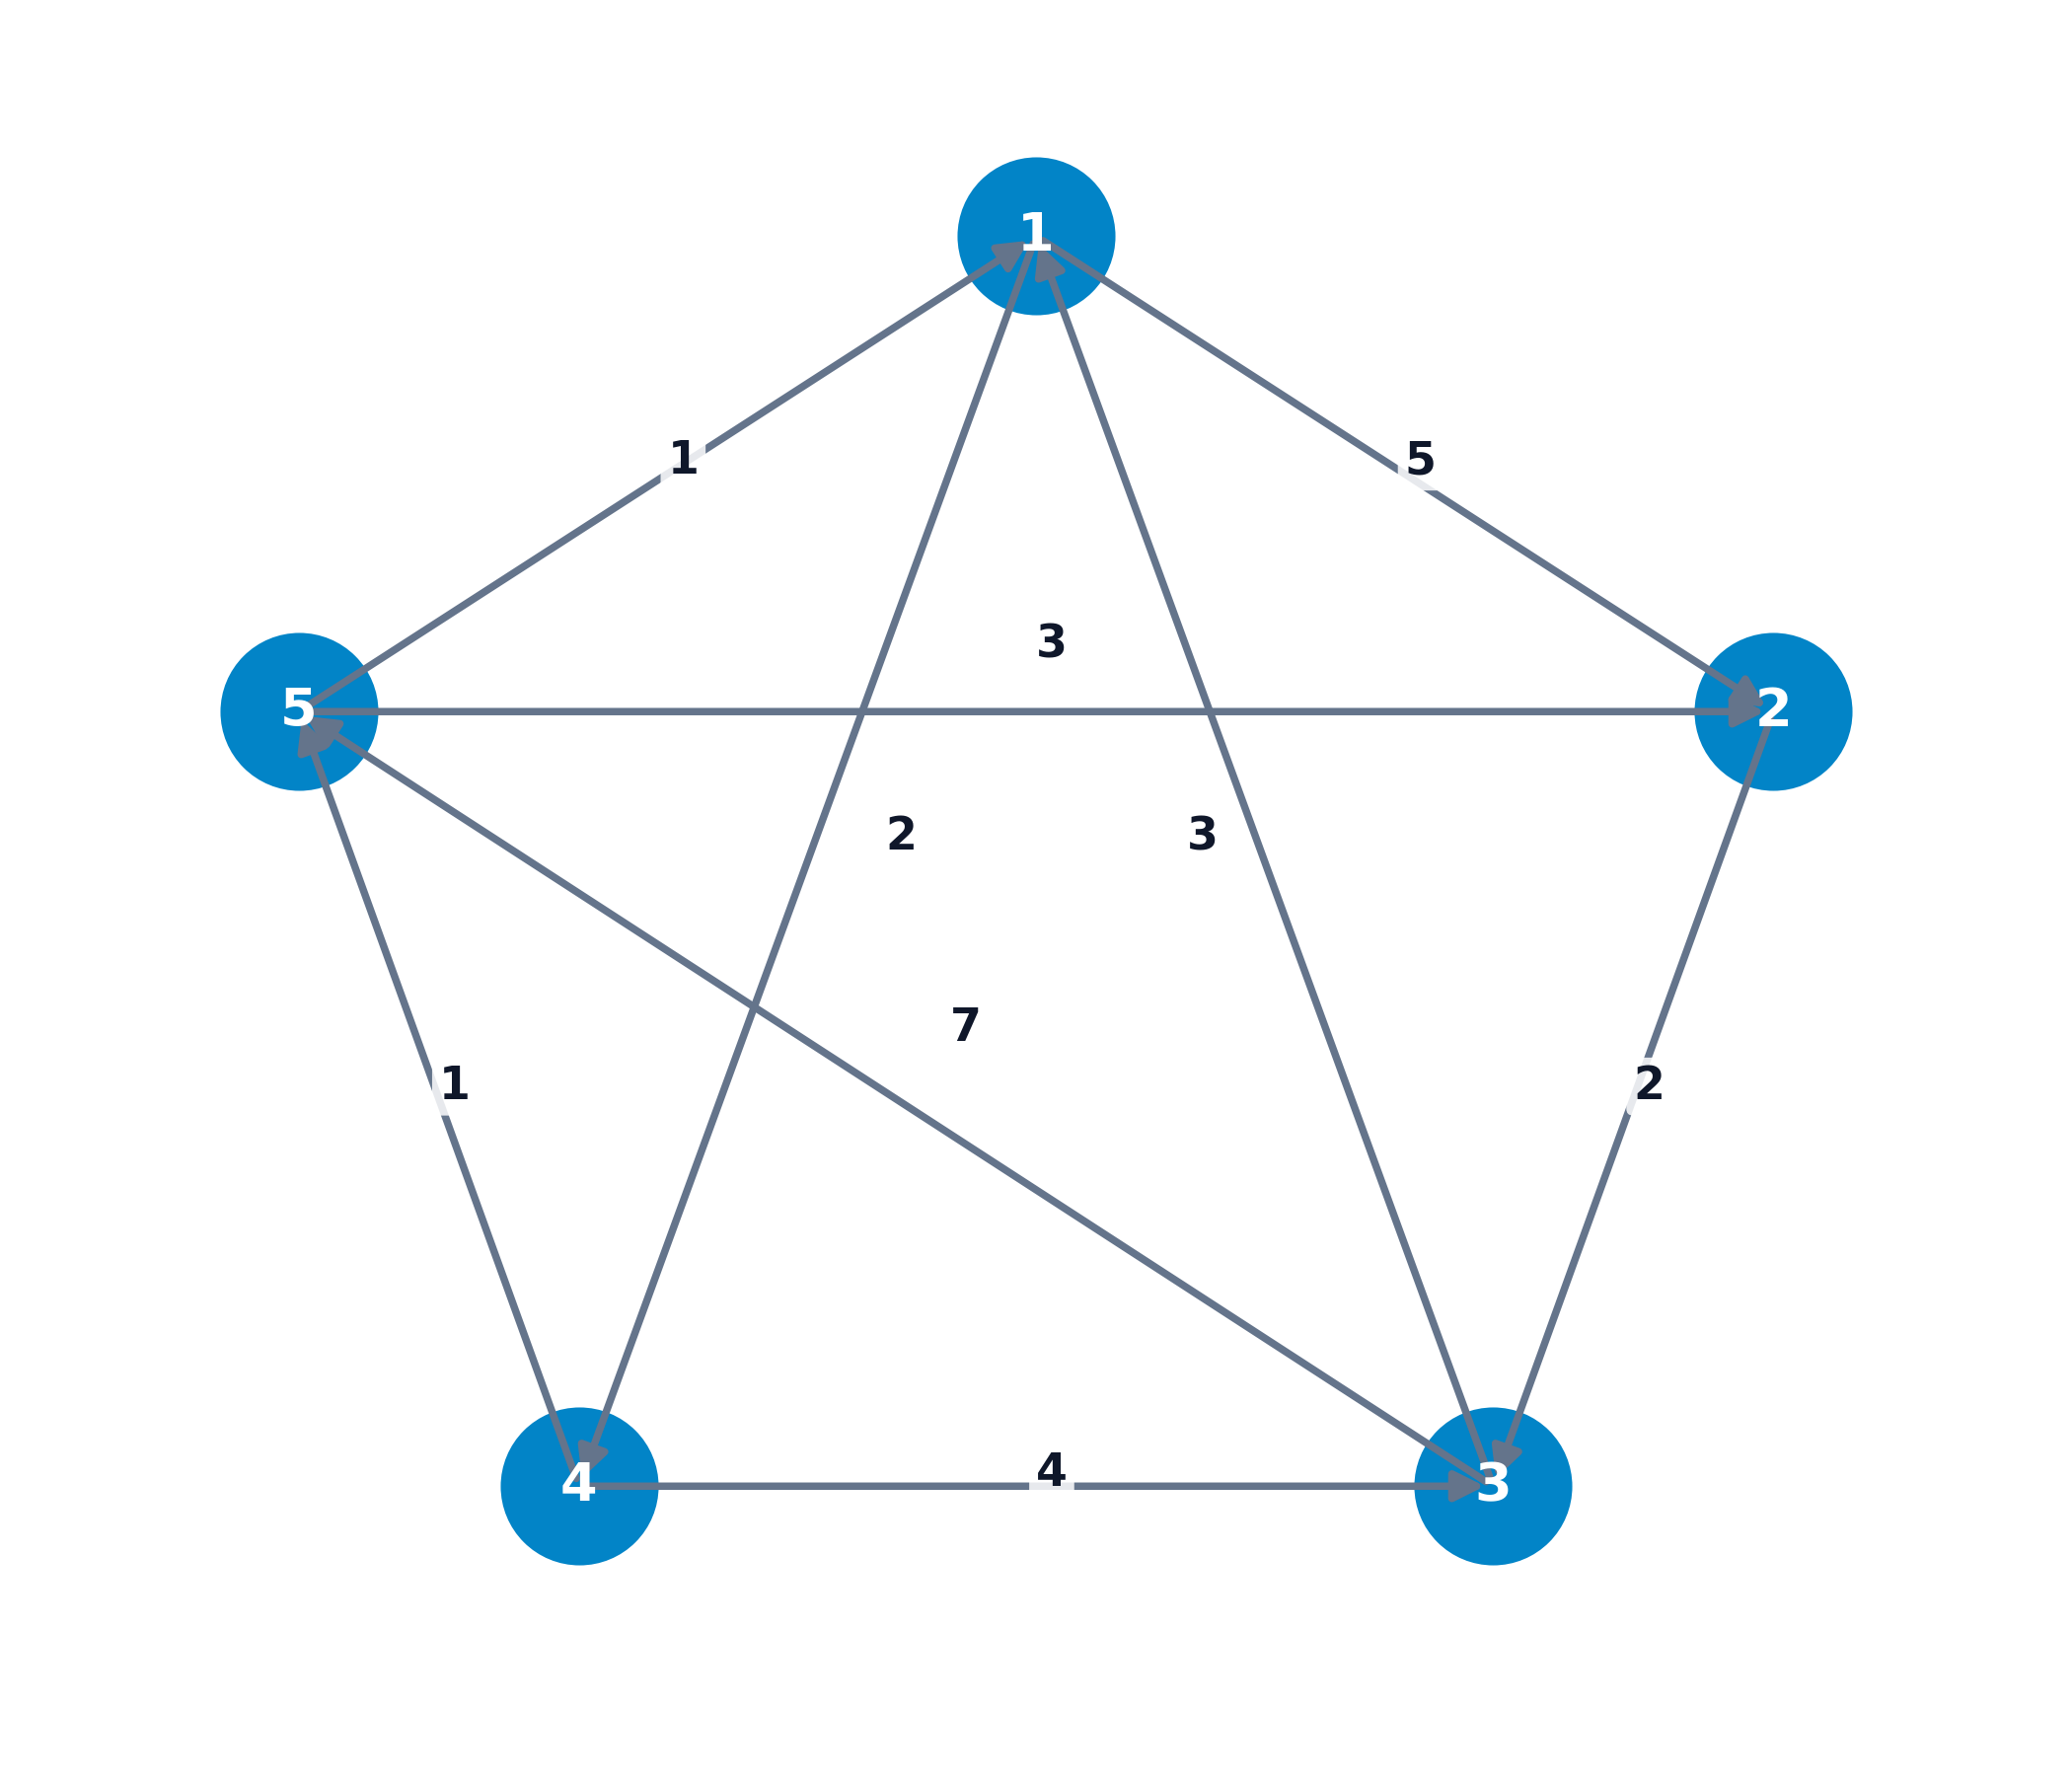
\includegraphics[width=0.65\linewidth,height=\textheight,keepaspectratio]{images/floyd_warshall_ejemplo_5nodos.png}

}

\caption{\label{fig-floyd-warshall-ejemplo-5nodos}Digrafo valorado de 5
nodos para el ejemplo del Algoritmo de Floyd-Warshall}

\end{figure}%

\textbf{1. Matriz Inicial \(D^{(0)}\) (Distancias directas de los
arcos)}: \[
D^{(0)} = \begin{pmatrix}
0 & 5 & \infty & 2 & \infty \\
\infty & 0 & 2 & \infty & \infty \\
3 & \infty & 0 & \infty & 7 \\
\infty & \infty & 4 & 0 & 1 \\
1 & 3 & \infty & \infty & 0
\end{pmatrix}
\]

\textbf{2. Iteración \(k=1\) (Permitir el nodo 1 como vértice
intermedio)}: Se evalúa
\(d_{ij}^{(1)} = \min \{ d_{ij}^{(0)}, d_{i1}^{(0)} + d_{1j}^{(0)} \}\).
La fila 1 \((0, 5, \infty, 2, \infty)\) y la columna 1
\((0, \infty, 3, \infty, 1)^T\) permiten actualizar los siguientes
elementos:

\begin{itemize}
\tightlist
\item
  \(d_{32}^{(1)} = \min \{ \infty, 3 + 5 \} = 8\).
\item
  \(d_{34}^{(1)} = \min \{ \infty, 3 + 2 \} = 5\).
\item
  \(d_{54}^{(1)} = \min \{ \infty, 1 + 2 \} = 3\).
\end{itemize}

\[
D^{(1)} = \begin{pmatrix}
0 & 5 & \infty & 2 & \infty \\
\infty & 0 & 2 & \infty & \infty \\
3 & \textcolor{forestgreen}{\mathbf{8}} & 0 & \textcolor{forestgreen}{\mathbf{5}} & 7 \\
\infty & \infty & 4 & 0 & 1 \\
1 & 3 & \infty & \textcolor{forestgreen}{\mathbf{3}} & 0
\end{pmatrix}
\]

\textbf{3. Iteración \(k=2\) (Permitir el nodo 2 como vértice
intermedio)}: Evaluando combinaciones a través de la fila 2
\((\infty, 0, 2, \infty, \infty)\) y la columna 2
\((5, 0, 8, \infty, 3)^T\):

\begin{itemize}
\tightlist
\item
  \(d_{13}^{(2)} = \min \{ \infty, 5 + 2 \} = 7\).
\item
  \(d_{53}^{(2)} = \min \{ \infty, 3 + 2 \} = 5\).
\end{itemize}

\[
D^{(2)} = \begin{pmatrix}
0 & 5 & \textcolor{forestgreen}{\mathbf{7}} & 2 & \infty \\
\infty & 0 & 2 & \infty & \infty \\
3 & 8 & 0 & 5 & 7 \\
\infty & \infty & 4 & 0 & 1 \\
1 & 3 & \textcolor{forestgreen}{\mathbf{5}} & 3 & 0
\end{pmatrix}
\]

\textbf{4. Iteración \(k=3\) (Permitir el nodo 3 como vértice
intermedio)}: Evaluando combinaciones a través de la fila 3
\((3, 8, 0, 5, 7)\) y la columna 3 \((7, 2, 0, 4, 5)^T\):

\begin{itemize}
\tightlist
\item
  \(d_{15}^{(3)} = \min \{ \infty, 7 + 7 \} = 14\).
\item
  \(d_{21}^{(3)} = \min \{ \infty, 2 + 3 \} = 5\),
  \(d_{24}^{(3)} = \min \{ \infty, 2 + 5 \} = 7\),
  \(d_{25}^{(3)} = \min \{ \infty, 2 + 7 \} = 9\).
\item
  \(d_{41}^{(3)} = \min \{ \infty, 4 + 3 \} = 7\),
  \(d_{42}^{(3)} = \min \{ \infty, 4 + 8 \} = 12\).
\end{itemize}

\[
D^{(3)} = \begin{pmatrix}
0 & 5 & 7 & 2 & \textcolor{forestgreen}{\mathbf{14}} \\
\textcolor{forestgreen}{\mathbf{5}} & 0 & 2 & \textcolor{forestgreen}{\mathbf{7}} & \textcolor{forestgreen}{\mathbf{9}} \\
3 & 8 & 0 & 5 & 7 \\
\textcolor{forestgreen}{\mathbf{7}} & \textcolor{forestgreen}{\mathbf{12}} & 4 & 0 & 1 \\
1 & 3 & 5 & 3 & 0
\end{pmatrix}
\]

\textbf{5. Iteración \(k=4\) (Permitir el nodo 4 como vértice
intermedio)}: Evaluando combinaciones a través de la fila 4
\((7, 12, 4, 0, 1)\) y la columna 4 \((2, 7, 5, 0, 3)^T\):

\begin{itemize}
\tightlist
\item
  \(d_{13}^{(4)} = \min \{ 7, 2 + 4 \} = 6\),
  \(d_{15}^{(4)} = \min \{ 14, 2 + 1 \} = 3\).
\item
  \(d_{25}^{(4)} = \min \{ 9, 7 + 1 \} = 8\).
\item
  \(d_{35}^{(4)} = \min \{ 7, 5 + 1 \} = 6\).
\end{itemize}

\[
D^{(4)} = \begin{pmatrix}
0 & 5 & \textcolor{forestgreen}{\mathbf{6}} & 2 & \textcolor{forestgreen}{\mathbf{3}} \\
5 & 0 & 2 & 7 & \textcolor{forestgreen}{\mathbf{8}} \\
3 & 8 & 0 & 5 & \textcolor{forestgreen}{\mathbf{6}} \\
7 & 12 & 4 & 0 & 1 \\
1 & 3 & 5 & 3 & 0
\end{pmatrix}
\]

\textbf{6. Iteración \(k=5\) (Permitir el nodo 5 como vértice
intermedio)}: Evaluando combinaciones a través de la fila 5
\((1, 3, 5, 3, 0)\) y la columna 5 \((3, 8, 6, 1, 0)^T\):

\begin{itemize}
\tightlist
\item
  \(d_{41}^{(5)} = \min \{ 7, 1 + 1 \} = 2\),
  \(d_{42}^{(5)} = \min \{ 12, 1 + 3 \} = 4\).
\end{itemize}

\[
D^{(5)} = \begin{pmatrix}
0 & 5 & 6 & 2 & 3 \\
5 & 0 & 2 & 7 & 8 \\
3 & 8 & 0 & 5 & 6 \\
\textcolor{forestgreen}{\mathbf{2}} & \textcolor{forestgreen}{\mathbf{4}} & 4 & 0 & 1 \\
1 & 3 & 5 & 3 & 0
\end{pmatrix}
\]

Parada en \(k = 5\). La matriz final \(D^{(5)}\) proporciona las
distancias mínimas absolutas entre todo par de nodos \(i, j \in V\). La
animación iterativa y las arborescencias resultantes se ilustran en la
Figura~\ref{fig-floyd-warshall-ejemplo-pasos}.

\begin{figure}[H]

\centering{

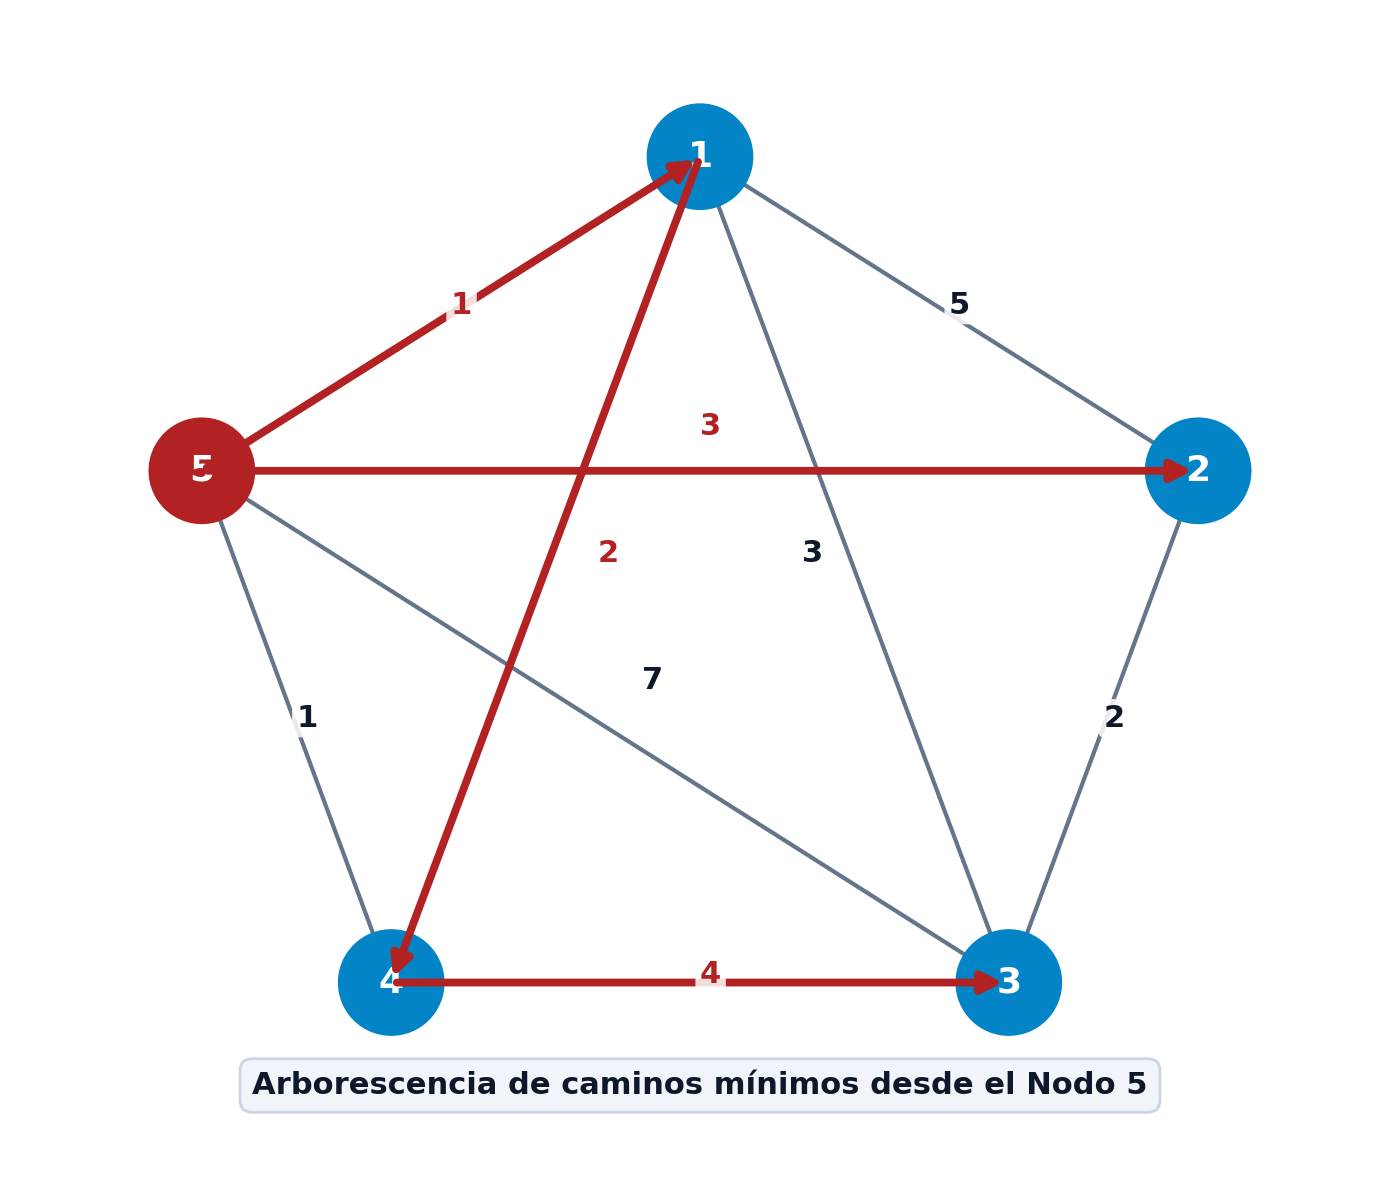
\includegraphics[width=0.75\linewidth,height=\textheight,keepaspectratio]{images/floyd_warshall_traza_paso_a_paso.png}

}

\caption{\label{fig-floyd-warshall-ejemplo-pasos}Traza gráfica de las
arborescencias de caminos mínimos en el Algoritmo de Floyd-Warshall}

\end{figure}%

\end{tcolorbox}

\chapter{Flujos en redes}\label{flujos-en-redes}

La optimización de \textbf{flujos en redes} constituye uno de los
pilares más avanzados y de mayor aplicabilidad en el análisis de redes y
la investigación operativa. Permite modelar, cuantificar y optimizar la
circulación de bienes físicos o abstractos (tales como tráfico
vehicular, fluidos en tuberías, corriente eléctrica, paquetes de
información o transferencias financieras) a través de infraestructuras
interconectadas sujetas a capacidades físicas límite (Ahuja, Magnanti, y
Orlin 1993; Bertsekas 1998).

En este capítulo desarrollaremos la fundamentación matemática rigurosa
de la teoría de flujos. Comenzaremos con el estudio algebraico del
espacio de flujos, ciclos y cociclos (cortes), introduciendo el célebre
Lema de Coloración de Arcos de Minty como piedra angular demostrativa. A
continuación, formularemos el problema del flujo máximo, demostrando
formalmente el Teorema Max-Flow Min-Cut de Ford-Fulkerson y analizando
sus algoritmos de resolución. Finalmente, ampliaremos la teoría a la
formulación mediante programación lineal dual y a la resolución del
problema de flujo a coste mínimo y el problema general del transbordo.

\begin{tcolorbox}[enhanced jigsaw, toprule=.15mm, opacitybacktitle=0.6, coltitle=black, colbacktitle=quarto-callout-important-color!10!white, title=\textcolor{quarto-callout-important-color}{\faExclamation}\hspace{0.5em}{Objetivos de aprendizaje}, arc=.35mm, rightrule=.15mm, toptitle=1mm, breakable, bottomtitle=1mm, titlerule=0mm, colback=white, opacityback=0, leftrule=.75mm, colframe=quarto-callout-important-color-frame, left=2mm, bottomrule=.15mm]

Al finalizar este capítulo, serás capaz de:

\begin{enumerate}
\def\labelenumi{\arabic{enumi}.}
\tightlist
\item
  \textbf{Formular} algebraicamente el concepto de flujo y circulación
  en digrafos mediante las ecuaciones de conservación y balance en los
  nodos.
\item
  \textbf{Caracterizar} la estructura vectorial de los flujos,
  calculando las bases fundamentales de ciclos y el número ciclomático
  \(\nu(G)\).
\item
  \textbf{Demostrar} y \textbf{aplicar} el Lema de Coloración de Arcos
  de Minty mediante su algoritmo constructivo de etiquetado de vértices.
\item
  \textbf{Demostrar} y \textbf{analizar} el Teorema de Flujo Máximo -
  Corte Mínimo de Ford-Fulkerson y la relación de dualidad en
  optimización lineal.
\item
  \textbf{Ejecutar} y \textbf{caracterizar} el algoritmo de
  Ford-Fulkerson en redes residuales mediante el método de etiquetado
  directo y la cota de Edmonds-Karp.
\item
  \textbf{Formular} y \textbf{resolver} los problemas de flujo a coste
  mínimo y el problema general del transbordo.
\end{enumerate}

\end{tcolorbox}

\section{Estructura algebraica de flujos, ciclos y
cociclos}\label{estructura-algebraica-de-flujos-ciclos-y-cociclos}

El análisis cualitativo y cuantitativo de las redes de flujo requiere
establecer una representación matemática rigurosa basada en el álgebra
lineal sobre la topología del digrafo. Los flujos en una red no son
simples colecciones arbitrarias de números asignados a las conexiones;
responden a leyes físicas y topológicas estrictas de conservación local
en los vértices (análogas a las leyes de Kirchhoff en circuitos
eléctricos o a la ecuación de continuidad en dinámica de fluidos).

Para formalizar este comportamiento, representamos la red como un
digrafo conexo \(G = (V, U)\) formado por un conjunto de \(n = |V|\)
vértices y \(m = |U|\) arcos dirigidos.

\begin{tcolorbox}[enhanced jigsaw, toprule=.15mm, opacitybacktitle=0.6, coltitle=black, colbacktitle=quarto-callout-note-color!10!white, title=\textcolor{quarto-callout-note-color}{\faInfo}\hspace{0.5em}{Definición: Flujo en un digrafo y conservación}, arc=.35mm, rightrule=.15mm, toptitle=1mm, breakable, bottomtitle=1mm, titlerule=0mm, colback=white, opacityback=0, leftrule=.75mm, colframe=quarto-callout-note-color-frame, left=2mm, bottomrule=.15mm]

Dado un digrafo conexo \(G = (V, U)\) con \(m\) arcos dirigidos, un
\textbf{flujo} es un vector
\(\mathbf{f} = (f_{u_1}, f_{u_2}, \dots, f_{u_m})^T \in \mathbb{R}^m\)
cuyas componentes representan la cantidad de caudal o flujo \(f_u\) que
transita por cada arco \(u \in U\), satisfaciendo la \textbf{ley de
conservación de flujo} en todos los vértices:

\[
\sum_{u \in w^+(i)} f_u = \sum_{u \in w^-(i)} f_u, \quad \forall i \in V
\]

donde \(w^+(i)\) representa el conjunto de arcos salientes del nodo
\(i\) y \(w^-(i)\) el conjunto de arcos entrantes al nodo \(i\).

\end{tcolorbox}

\begin{tcolorbox}[enhanced jigsaw, toprule=.15mm, opacitybacktitle=0.6, coltitle=black, colbacktitle=quarto-callout-note-color!10!white, title=\textcolor{quarto-callout-note-color}{\faInfo}\hspace{0.5em}{Nota de notación: Distinción entre arcos, vectores y componentes}, arc=.35mm, rightrule=.15mm, toptitle=1mm, breakable, bottomtitle=1mm, titlerule=0mm, colback=white, opacityback=0, leftrule=.75mm, colframe=quarto-callout-note-color-frame, left=2mm, bottomrule=.15mm]

Para evitar cualquier confusión entre los nombres de los arcos y los
valores numéricos del flujo:

\begin{enumerate}
\def\labelenumi{\arabic{enumi}.}
\tightlist
\item
  \textbf{Identificador del Arco}: Los \(m\) arcos del digrafo se
  etiquetan como \(u_1, u_2, \dots, u_m \in U\) (o bien por el par
  ordenado de sus vértices \(u = (i, j)\)).
\item
  \textbf{Identificador de Vectores (Superíndices)}: Los distintos
  vectores de flujo o de ciclo se denotan en negrita utilizando
  \textbf{superíndices} (por ejemplo,
  \(\mathbf{f}^1, \mathbf{f}^2, \mathbf{f}^3\) para vectores de flujo;
  \(\mathbf{\mu}^1, \mathbf{\mu}^2\) para vectores de ciclo).
\item
  \textbf{Componentes Escalares de Arco (Subíndices)}: El caudal que
  circula por el arco \(u_k\) se denota mediante el \textbf{subíndice}
  \(f_{u_k}\) (o \(f_{ij}\)), correspondiente a la \(k\)-ésima entrada
  del vector \(\mathbf{f}\). En los gráficos de la red, las etiquetas
  especifican explícitamente el arco y su valor (\(u_k: f_{u_k}\)).
\end{enumerate}

\end{tcolorbox}

En modelos generales de redes donde existen inyecciones o extracciones
externas de caudal (por ejemplo, plantas de generación o centros de
distribución), se asocia a cada nodo \(i \in V\) un escalar de balance
\(b_i \in \mathbb{R}\):

\begin{itemize}
\tightlist
\item
  \textbf{Nodo fuente (\(b_i > 0\))}: Inyecta \(b_i\) unidades netas de
  flujo a la red.
\item
  \textbf{Nodo sumidero (\(b_i < 0\))}: Extrae \(|b_i|\) unidades netas
  de flujo de la red.
\item
  \textbf{Nodo de transbordo (\(b_i = 0\))}: La suma de flujos entrantes
  iguala exactamente a la de salientes, actuando como mero nodo de paso.
\end{itemize}

La condición necesaria de factibilidad global exige el equilibrio
perfecto entre oferta y demanda: la suma total de balances debe ser nula
en toda la red, \(\sum_{i \in V} b_i = 0\). Cuando la red no posee
entradas ni salidas externas (\(b_i = 0\) para todo \(i \in V\)), el
vector \(\mathbf{f}\) se denomina estrictamente \textbf{circulación},
garantizando la conservación exacta en cada vértice del digrafo.

\begin{tcolorbox}[enhanced jigsaw, toprule=.15mm, opacitybacktitle=0.6, coltitle=black, colbacktitle=quarto-callout-tip-color!10!white, title=\textcolor{quarto-callout-tip-color}{\faLightbulb}\hspace{0.5em}{Ejemplo: Evaluación de vectores de flujo en un digrafo}, arc=.35mm, rightrule=.15mm, toptitle=1mm, breakable, bottomtitle=1mm, titlerule=0mm, colback=white, opacityback=0, leftrule=.75mm, colframe=quarto-callout-tip-color-frame, left=2mm, bottomrule=.15mm]

Considérese el digrafo de 5 nodos \(V = \{a, b, c, d, e\}\) y 7 arcos
dirigidos
\(U = \{u_1=(a,b), u_2=(b,c), u_3=(c,d), u_4=(d,e), u_5=(e,a), u_6=(e,b), u_7=(e,c)\}\).

Se evalúan los siguientes tres vectores de flujo
\(\mathbf{f} \in \mathbb{R}^7\), ilustrados en la
Figura~\ref{fig-flujos-tres-vectores}:

\begin{enumerate}
\def\labelenumi{\arabic{enumi}.}
\tightlist
\item
  \(\mathbf{f}^1 = (2.7;\, 2;\, 2;\, 2;\, 2.7;\, -0.7;\, 0)^T\):

  \begin{itemize}
  \tightlist
  \item
    Nodo \(a\): Salen \(f_1 = 2.7\), entran
    \(f_5 = 2.7 \implies 2.7 = 2.7\).
  \item
    Nodo \(b\): Salen \(f_2 = 2\), entran
    \(f_1 + f_6 = 2.7 + (-0.7) = 2 \implies 2 = 2\).
  \item
    Nodo \(e\): Salen \(f_5 + f_6 + f_7 = 2.7 - 0.7 + 0 = 2\), entra
    \(f_4 = 2 \implies 2 = 2\).
  \item
    \emph{Conclusión}: Cumple la ley de conservación en todos los nodos,
    luego \(\mathbf{f}^1\) es un flujo válido.
  \end{itemize}
\item
  \(\mathbf{f}^2 = (0;\, 1;\, 1;\, 1;\, 0;\, 1;\, 0)^T\): Corresponde al
  flujo que circula por el ciclo formado por los arcos
  \(u_2, u_3, u_4, u_6\).
\item
  \(\mathbf{f}^3 = (1;\, 0;\, -1;\, -1;\, 1;\, -1;\, -1)^T\): Satisface
  las ecuaciones de conservación en los 5 nodos.
\end{enumerate}

\begin{figure}[H]

\centering{

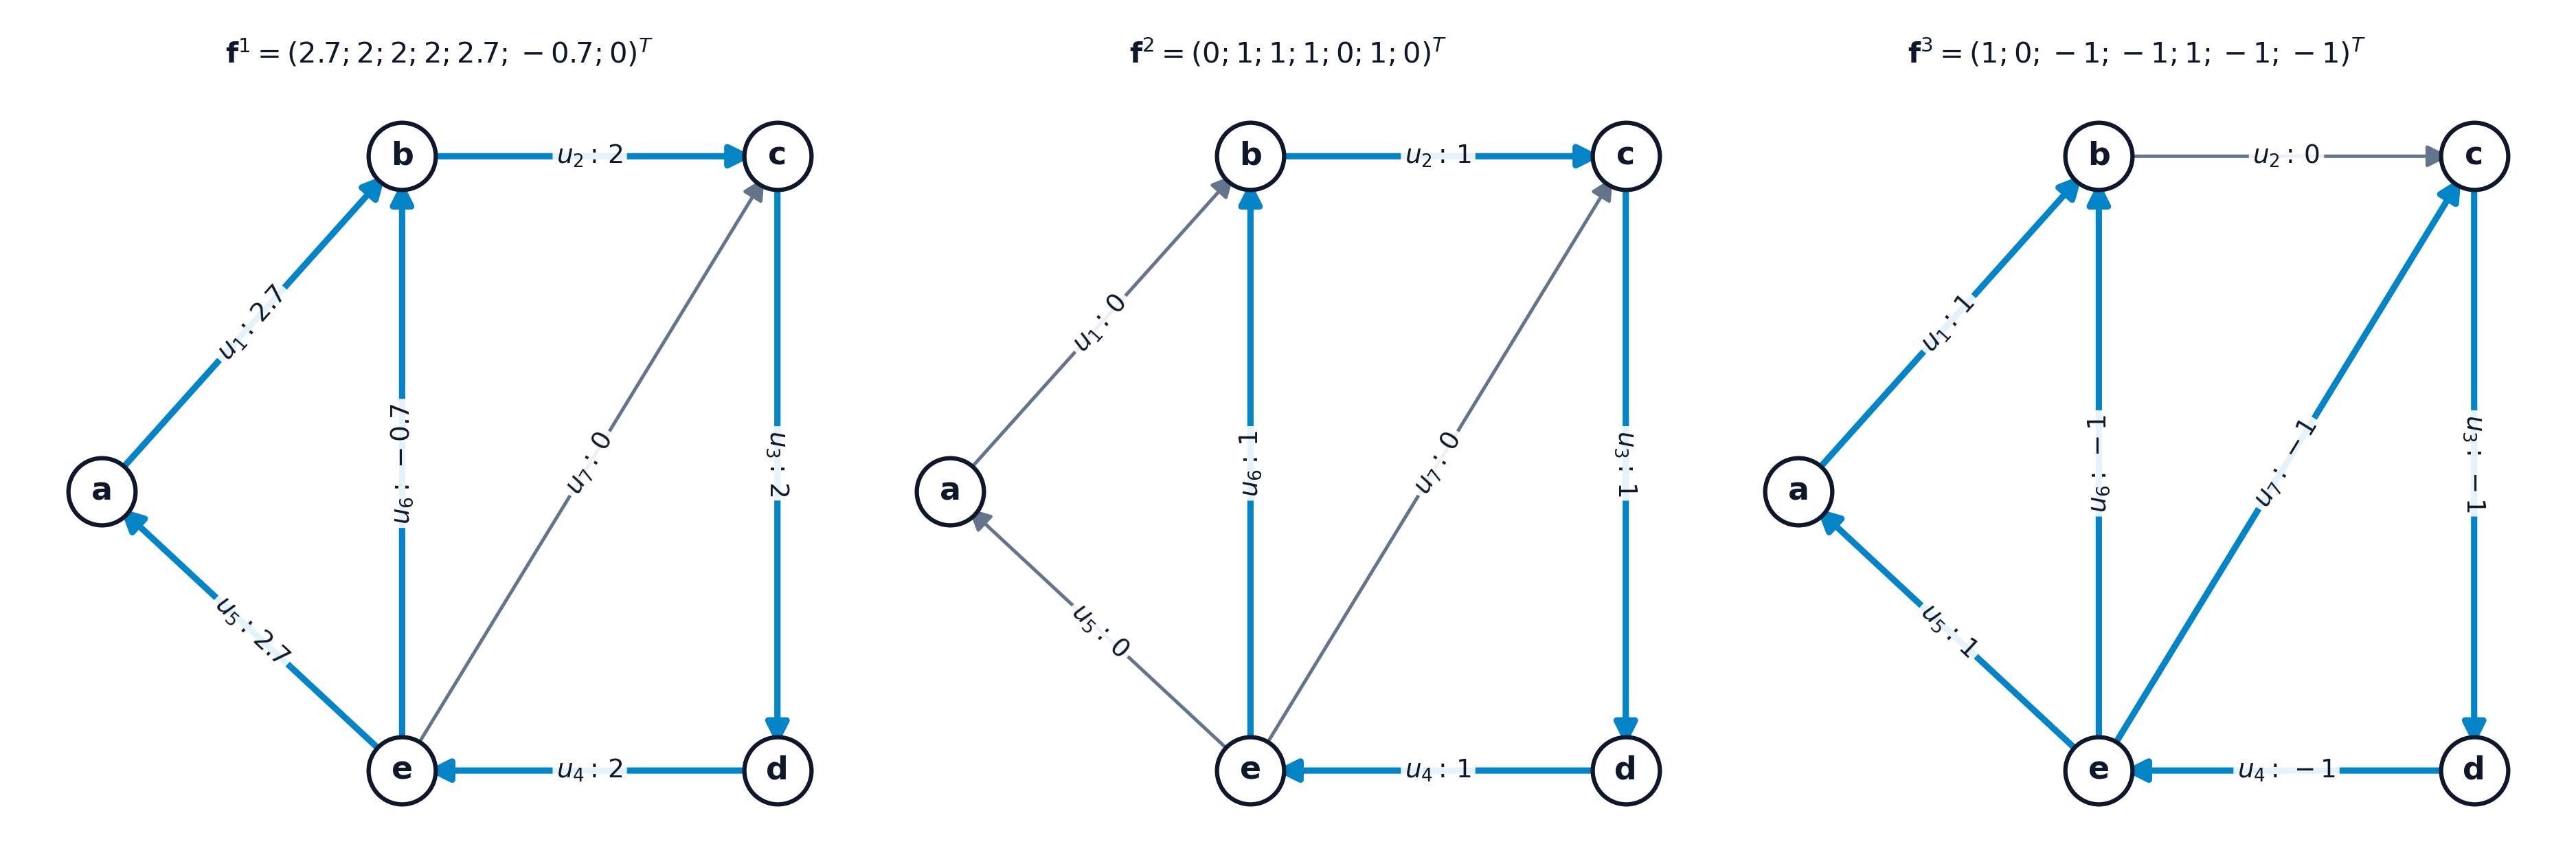
\includegraphics[width=0.85\linewidth,height=\textheight,keepaspectratio]{images/flujos_tres_vectores_ejemplo.png}

}

\caption{\label{fig-flujos-tres-vectores}Evaluación de tres vectores de
flujo sobre un digrafo de 5 nodos}

\end{figure}%

\end{tcolorbox}

La topología del digrafo impone restricciones fundamentales sobre los
vectores de flujo factibles. Por ejemplo, en una estructura sin
circuitos cerrados, la conservación obliga a que no pueda sostenerse
ningún caudal continuo.

\begin{tcolorbox}[enhanced jigsaw, toprule=.15mm, opacitybacktitle=0.6, coltitle=black, colbacktitle=quarto-callout-note-color!10!white, title=\textcolor{quarto-callout-note-color}{\faInfo}\hspace{0.5em}{Lema: Flujo nulo en árboles}, arc=.35mm, rightrule=.15mm, toptitle=1mm, breakable, bottomtitle=1mm, titlerule=0mm, colback=white, opacityback=0, leftrule=.75mm, colframe=quarto-callout-note-color-frame, left=2mm, bottomrule=.15mm]

Un flujo definido sobre un árbol (digrafo conexo acíclico) es
necesariamente el \textbf{flujo nulo} (\(\mathbf{f} = \mathbf{0}\)).

\emph{Demostración}: Todo árbol de \(n\) vértices posee \(n - 1\) arcos
y contiene al menos un vértice pendiente o hoja \(x_1\) de grado total
\(d(x_1) = 1\). Sea \(u \in U\) el único arco incidente en \(x_1\). Por
la ley de conservación de flujo en \(x_1\), la única componente entrante
o saliente debe ser cero, \(f_u = 0\).

Eliminando el nodo \(x_1\) y el arco \(u\), se obtiene un subgrafo
generado sobre \(V \setminus \{x_1\}\) que mantiene la estructura de
árbol. Repitiendo el razonamiento inductivo para los restantes \(n - 1\)
nodos, se deduce que todas las componentes del vector de flujo son cero:
\(f_u = 0, \forall u \in U\). \(\blacksquare\)

\end{tcolorbox}

El resultado anterior demuestra que la existencia de ciclos o circuitos
cerrados es una condición estrictamente necesaria para sostener una
circulación no nula en una red. Al añadir arcos a un árbol para formar
ciclos, las ecuaciones de conservación lineales permiten combinar
diferentes soluciones de flujo mediante operaciones de suma y
multiplicación por escalares. Esta propiedad algebraica fundamental se
formaliza en el siguiente resultado.

\begin{tcolorbox}[enhanced jigsaw, toprule=.15mm, opacitybacktitle=0.6, coltitle=black, colbacktitle=quarto-callout-note-color!10!white, title=\textcolor{quarto-callout-note-color}{\faInfo}\hspace{0.5em}{Lema: Estructura vectorial del espacio de flujos}, arc=.35mm, rightrule=.15mm, toptitle=1mm, breakable, bottomtitle=1mm, titlerule=0mm, colback=white, opacityback=0, leftrule=.75mm, colframe=quarto-callout-note-color-frame, left=2mm, bottomrule=.15mm]

Cualquier combinación lineal de flujos es un flujo. En consecuencia, el
conjunto de flujos definidos sobre un digrafo \(G = (V, U)\) forma un
espacio vectorial.

\end{tcolorbox}

La estructura de espacio vectorial garantiza que el conjunto de flujos
satisface la clausura algebraica: sumar dos circulaciones factibles o
escalar una circulación existente produce siempre un flujo válido que
preserva la conservación en todos los vértices. Para ilustrar
cuantitativamente este principio abstracto, consideremos una combinación
lineal concreta de los vectores de flujo evaluados previamente.

\begin{tcolorbox}[enhanced jigsaw, toprule=.15mm, opacitybacktitle=0.6, coltitle=black, colbacktitle=quarto-callout-tip-color!10!white, title=\textcolor{quarto-callout-tip-color}{\faLightbulb}\hspace{0.5em}{Ejemplo: Combinación lineal de vectores de flujo}, arc=.35mm, rightrule=.15mm, toptitle=1mm, breakable, bottomtitle=1mm, titlerule=0mm, colback=white, opacityback=0, leftrule=.75mm, colframe=quarto-callout-tip-color-frame, left=2mm, bottomrule=.15mm]

Consideremos los tres vectores de flujo
\(\mathbf{f}^1, \mathbf{f}^2, \mathbf{f}^3 \in \mathbb{R}^7\) analizados
anteriormente sobre el digrafo de 5 nodos. Construimos la combinación
lineal:

\[
\mathbf{f} = 2\mathbf{f}^1 + \mathbf{f}^2 - 3\mathbf{f}^3
\]

Evaluando componente a componente:

\[
\begin{aligned}
\mathbf{f} &= 2(2.7;\, 2;\, 2;\, 2;\, 2.7;\, -0.7;\, 0)^T + (0;\, 1;\, 1;\, 1;\, 0;\, 1;\, 0)^T - 3(1;\, 0;\, -1;\, -1;\, 1;\, -1;\, -1)^T \\
&= (2.4;\, 5;\, 8;\, 8;\, 2.4;\, 2.6;\, 3)^T
\end{aligned}
\]

Como se ilustra en la Figura~\ref{fig-flujos-combinacion-lineal}, se
puede verificar fácilmente la conservación de flujo en cada uno de los 5
vértices:

\begin{itemize}
\tightlist
\item
  \textbf{Nodo \(a\)}: Salen \(f_1 = 2.4\), entran
  \(f_5 = 2.4 \implies 2.4 = 2.4\).
\item
  \textbf{Nodo \(b\)}: Salen \(f_2 = 5\), entran
  \(f_1 + f_6 = 2.4 + 2.6 = 5 \implies 5 = 5\).
\item
  \textbf{Nodo \(c\)}: Salen \(f_3 = 8\), entran
  \(f_2 + f_7 = 5 + 3 = 8 \implies 8 = 8\).
\item
  \textbf{Nodo \(d\)}: Salen \(f_4 = 8\), entran
  \(f_3 = 8 \implies 8 = 8\).
\item
  \textbf{Nodo \(e\)}: Salen \(f_5 + f_6 + f_7 = 2.4 + 2.6 + 3 = 8\),
  entra \(f_4 = 8 \implies 8 = 8\).
\end{itemize}

Por consiguiente, la combinación lineal \(\mathbf{f}\) satisface la
conservación en todos los nodos y constituye un flujo factible bien
definido.

\begin{figure}[H]

\centering{

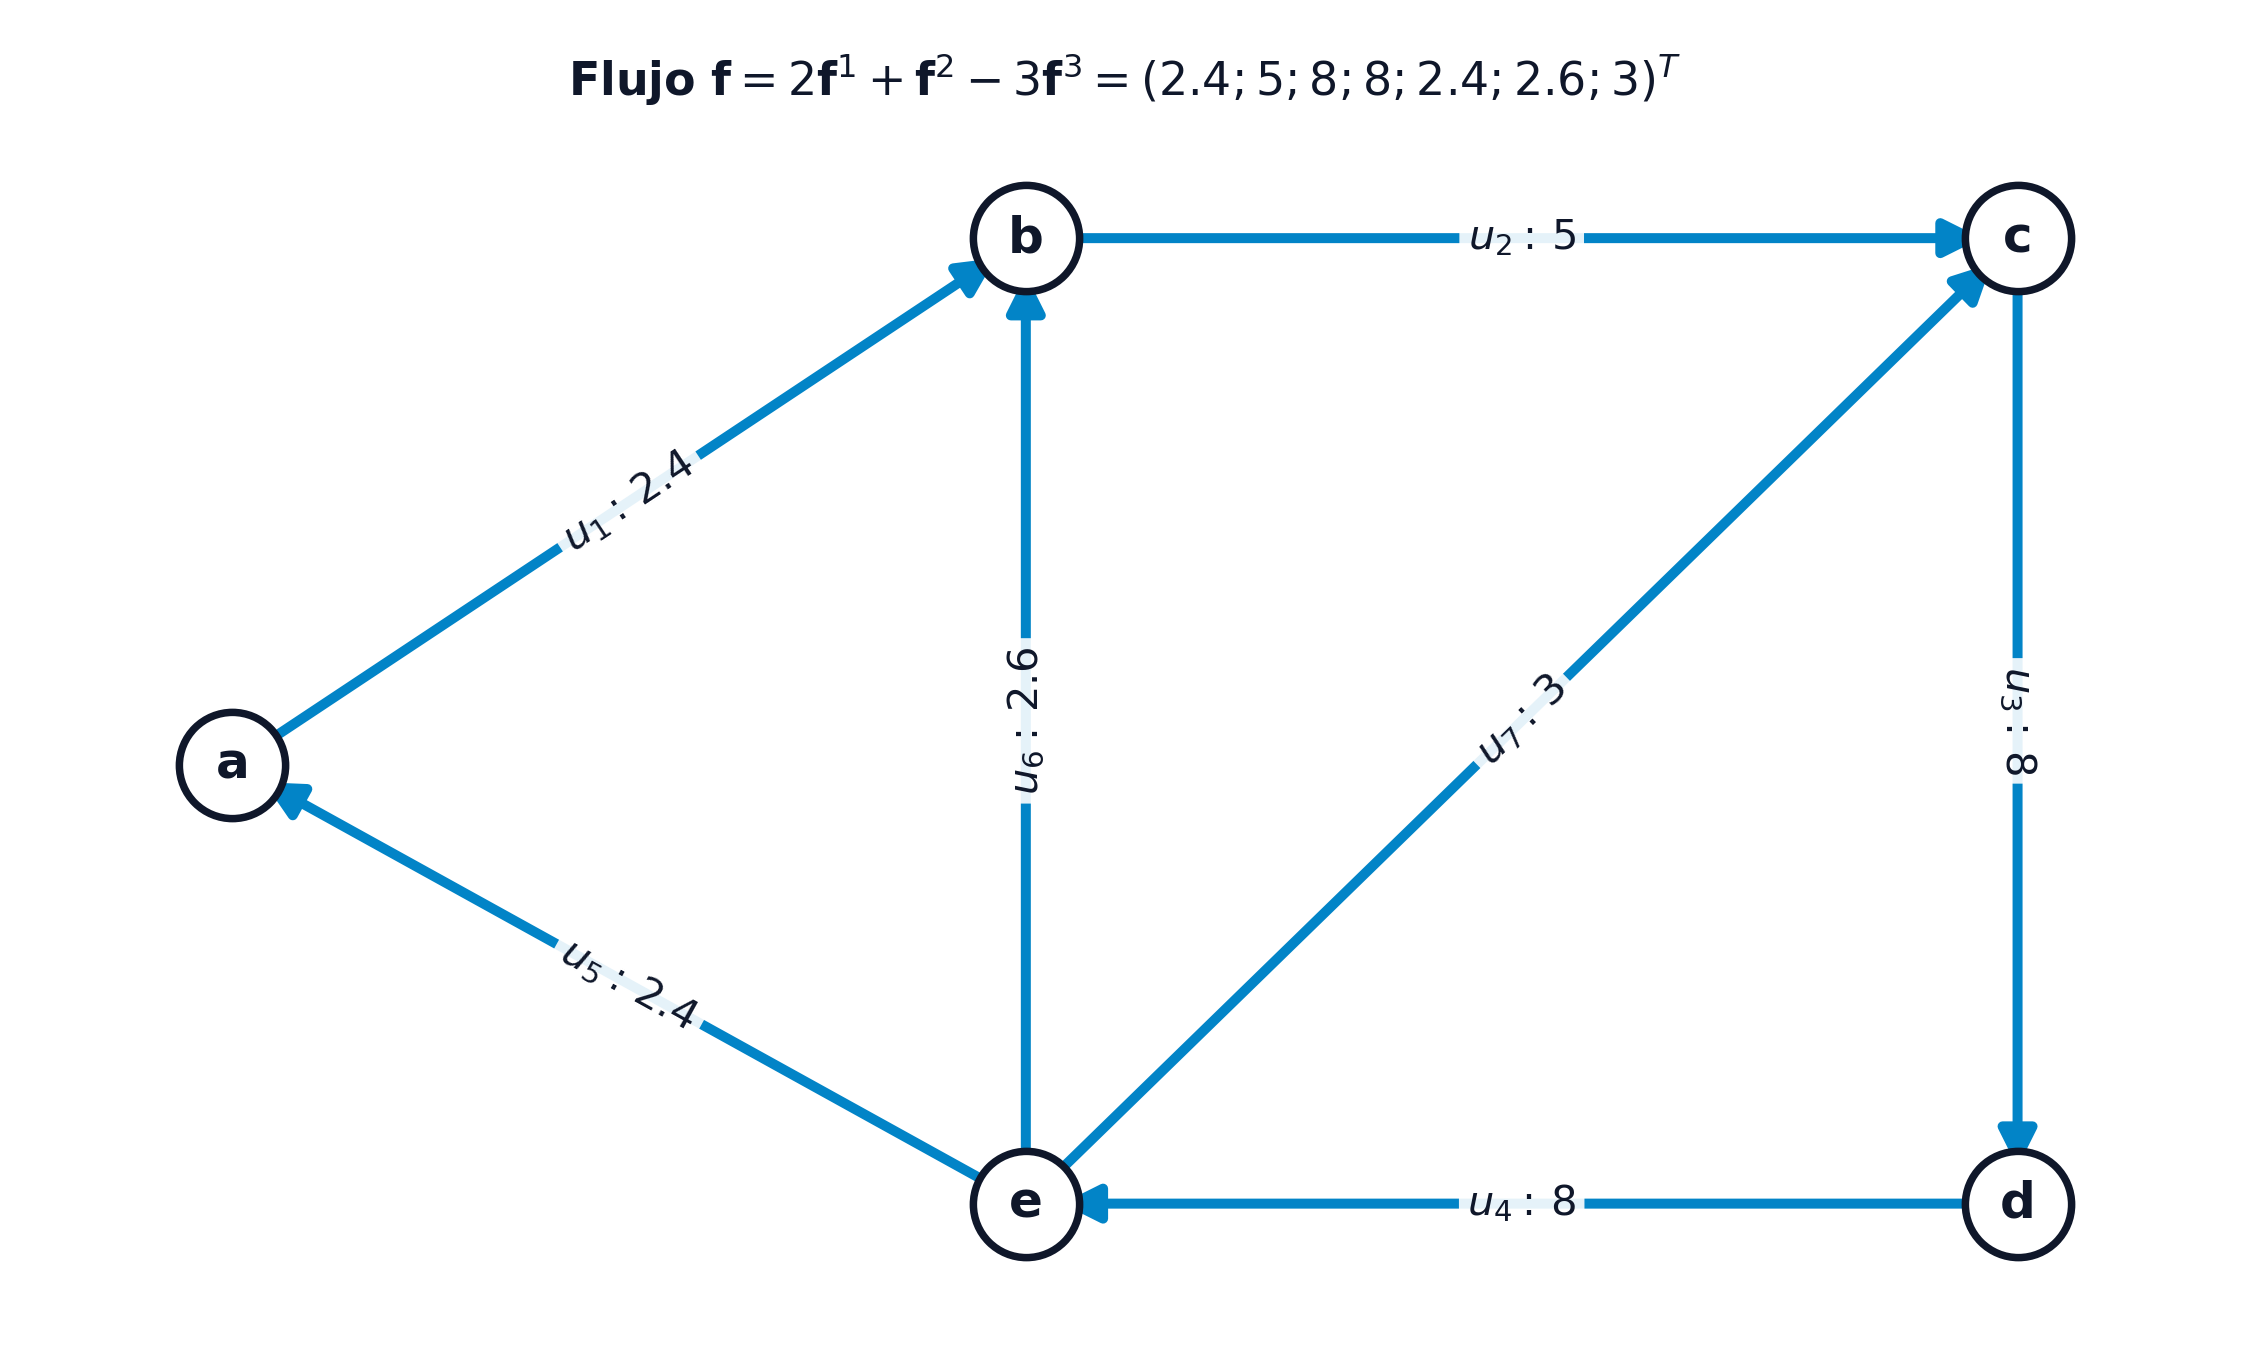
\includegraphics[width=0.6\linewidth,height=\textheight,keepaspectratio]{images/flujos_combinacion_lineal_ejemplo.png}

}

\caption{\label{fig-flujos-combinacion-lineal}Flujo resultante de la
combinación lineal
\(\mathbf{f} = 2\mathbf{f}^1 + \mathbf{f}^2 - 3\mathbf{f}^3\)}

\end{figure}%

\end{tcolorbox}

El resultado anterior prueba que el conjunto de flujos definidos sobre
un digrafo es un espacio vectorial. Para identificar su dimensión y una
base de flujos que permita caracterizarlos todos, es preciso estudiar la
relación que existe entre los ciclos y los flujos de un digrafo.

\subsection{Ciclos y su relación con los
flujos}\label{ciclos-y-su-relaciuxf3n-con-los-flujos}

Dado un digrafo conexo \(G = (V, U)\), un \textbf{ciclo} \(\mu\) es una
cadena simple (sin repetir arcos) cuyo nodo inicial y final coinciden.
Al dotar a \(\mu\) de un sentido de giro de referencia, los arcos
\(u \in \mu\) se clasifican en:

\begin{itemize}
\tightlist
\item
  \textbf{Arcos positivos (\(u \in \mu^+\))}: Su orientación en el
  digrafo coincide con el sentido del ciclo.
\item
  \textbf{Arcos negativos (\(u \in \mu^-\))}: Su orientación en el
  digrafo es opuesta al sentido del ciclo.
\item
  \textbf{Arcos fuera del ciclo (\(u \notin \mu\))}: No forman parte de
  la cadena simple.
\end{itemize}

A cada ciclo se le pueden asignar libremente dos orientaciones de giro
opuestas, lo que invierte los papeles de los arcos positivos y
negativos. Como se ilustra en la Figura~\ref{fig-ciclo-orientacion}, al
recorrer la red según un sentido de giro, los arcos \(1, 4, 3\) resultan
directos o positivos (\(\mu^+\)), mientras que los arcos \(6, 7\) son
opuestos o negativos (\(\mu^-\)).

\begin{figure}

\centering{

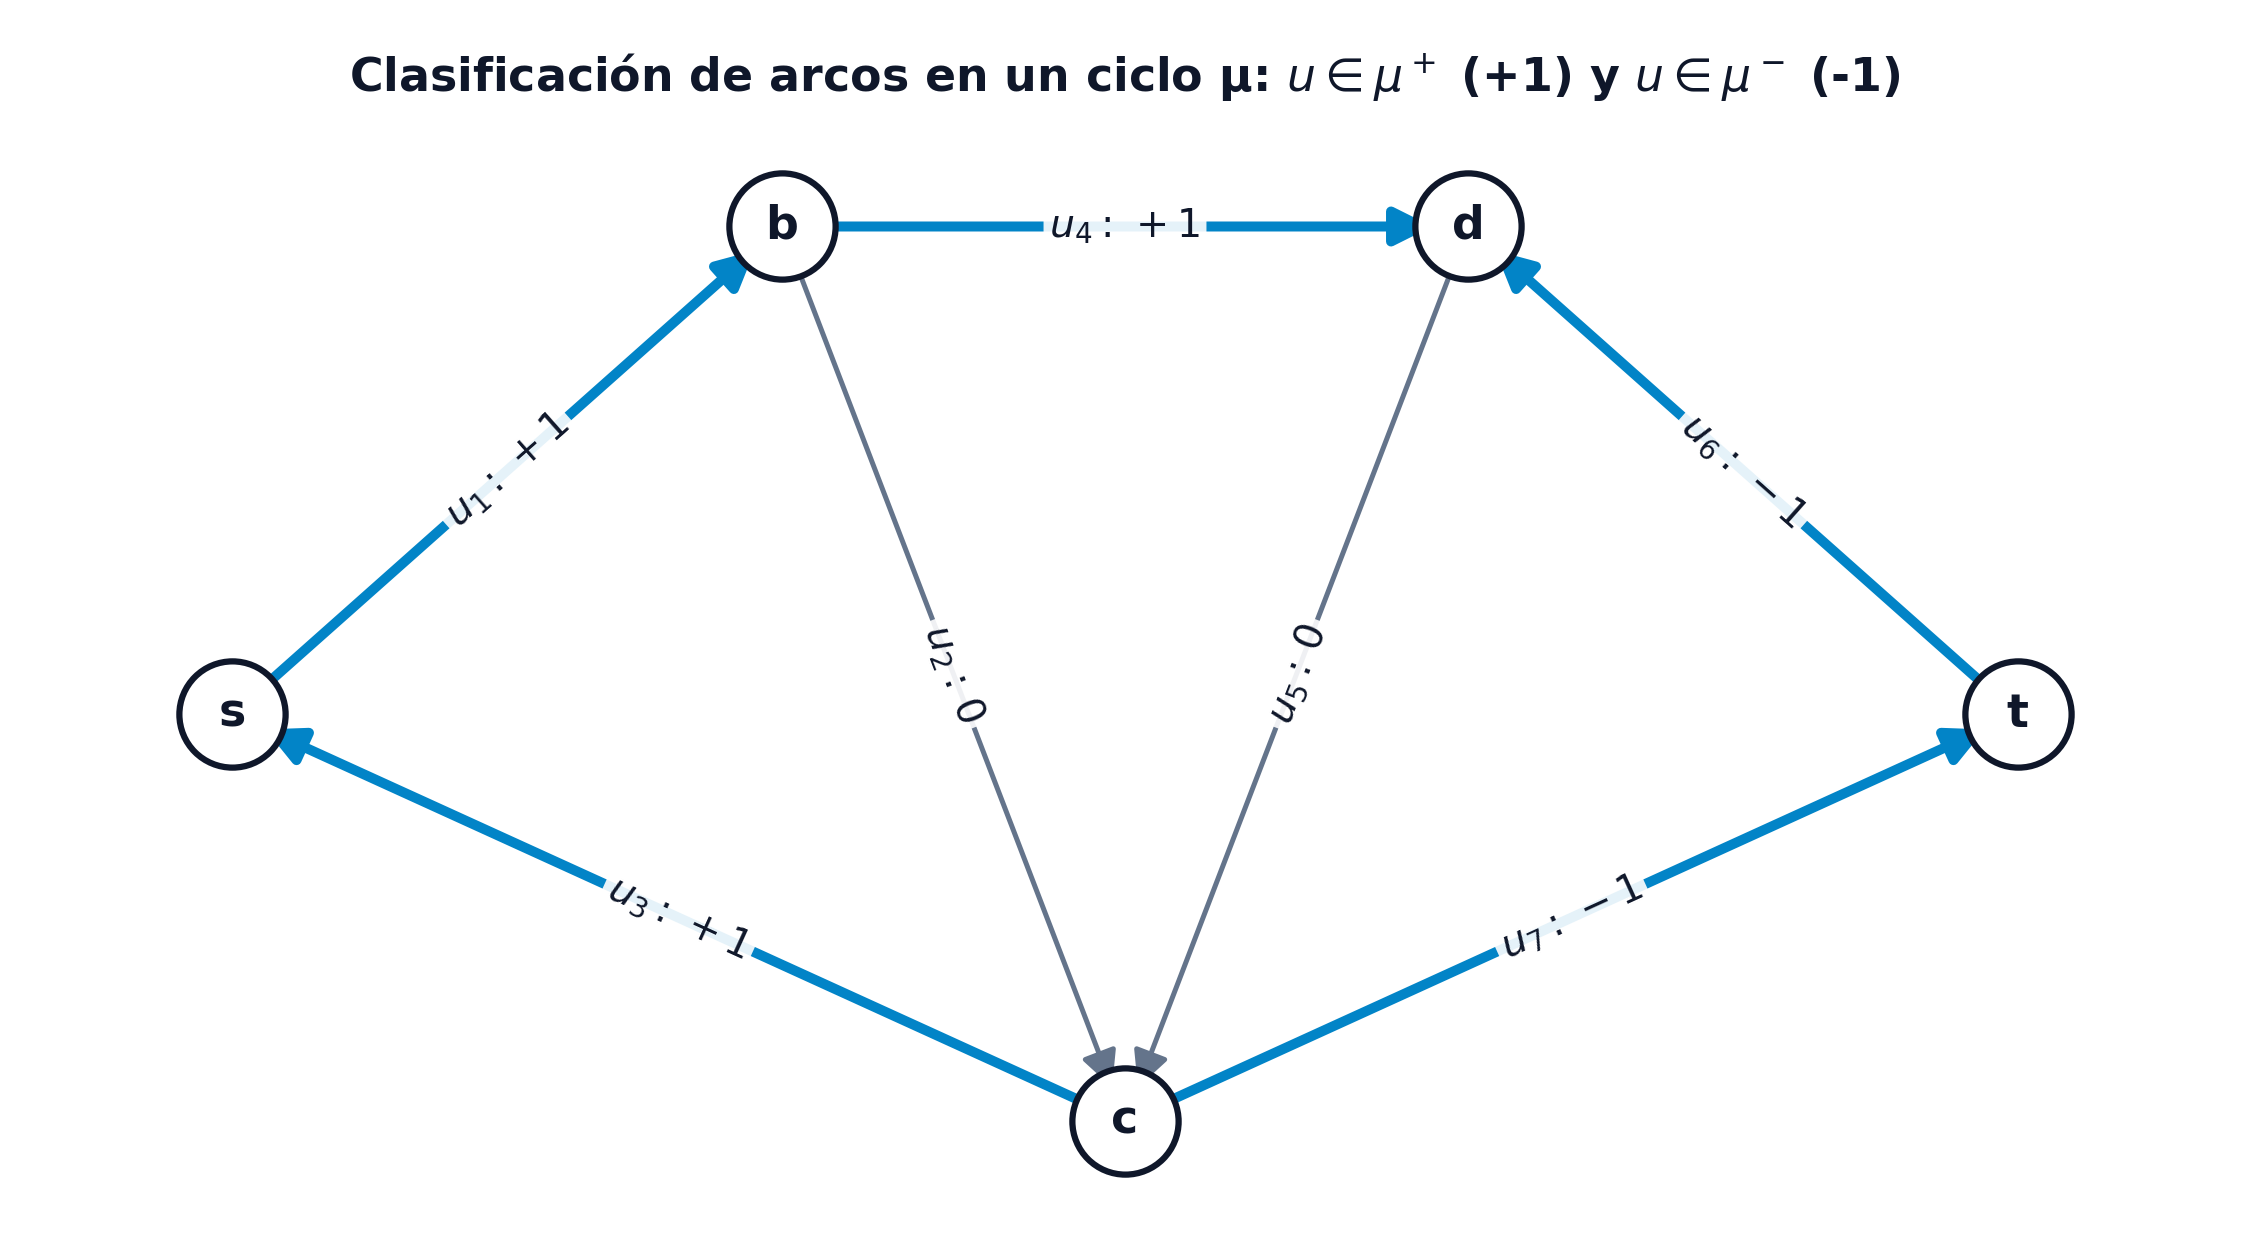
\includegraphics[width=0.65\linewidth,height=\textheight,keepaspectratio]{images/ciclo_orientacion_ejemplo.png}

}

\caption{\label{fig-ciclo-orientacion}Clasificación de arcos en un ciclo
\(\mu\) según el sentido de giro elegido}

\end{figure}%

\begin{tcolorbox}[enhanced jigsaw, toprule=.15mm, opacitybacktitle=0.6, coltitle=black, colbacktitle=quarto-callout-note-color!10!white, title=\textcolor{quarto-callout-note-color}{\faInfo}\hspace{0.5em}{Definición: Vector característico de un ciclo}, arc=.35mm, rightrule=.15mm, toptitle=1mm, breakable, bottomtitle=1mm, titlerule=0mm, colback=white, opacityback=0, leftrule=.75mm, colframe=quarto-callout-note-color-frame, left=2mm, bottomrule=.15mm]

Un ciclo \(\mu\) se representa algebraicamente mediante un vector
característico
\(\mathbf{\mu} = (\mu_1, \mu_2, \dots, \mu_m)^T \in \mathbb{R}^m\),
donde la componente asociada a cada arco \(u \in U\) se define como:

\[
\mu_u = \begin{cases}
+1 & \text{si } u \in \mu^+ \\
-1 & \text{si } u \in \mu^- \\
0 & \text{si } u \notin \mu
\end{cases}
\]

\end{tcolorbox}

\begin{tcolorbox}[enhanced jigsaw, toprule=.15mm, opacitybacktitle=0.6, coltitle=black, colbacktitle=quarto-callout-tip-color!10!white, title=\textcolor{quarto-callout-tip-color}{\faLightbulb}\hspace{0.5em}{Ejemplo: Vectores característicos de ciclos y relaciones lineales}, arc=.35mm, rightrule=.15mm, toptitle=1mm, breakable, bottomtitle=1mm, titlerule=0mm, colback=white, opacityback=0, leftrule=.75mm, colframe=quarto-callout-tip-color-frame, left=2mm, bottomrule=.15mm]

Considérese el digrafo de referencia de 5 nodos \(s, b, c, d, t\) y 7
arcos dirigidos de la Figura~\ref{fig-ciclos-vectores}. Se pueden
identificar diversos ciclos y sus correspondientes vectores
característicos \(\mathbf{\mu}_k \in \mathbb{R}^7\):

\begin{itemize}
\tightlist
\item
  \(\mathbf{\mu}_1 = (1, 1, 1, 0, 0, 0, 0)^T\): Ciclo orientado
  \(s \to b \to c \to s\) (formado por los arcos \(1, 2, 3\)).
\item
  \(\mathbf{\mu}_2 = (0, -1, 0, 1, 1, 0, 0)^T\): Ciclo
  \(b \to d \to c \to b\) (formado por los arcos \(4, 5\) y el opuesto
  de \(2\)).
\item
  \(\mathbf{\mu}_3 = (1, 0, 1, 1, 1, 0, 0)^T\): Ciclo exterior
  \(s \to b \to d \to c \to s\).
\item
  \(\mathbf{\mu}_4 = (-1, -1, -1, 0, -1, -1, -1)^T\): Ciclo global en
  sentido opuesto.
\item
  \(\mathbf{\mu}_5 = (-1, -1, -1, 0, 0, 0, 0)^T\): Ciclo inverso al
  ciclo \(\mathbf{\mu}_1\).
\end{itemize}

\begin{figure}[H]

\centering{

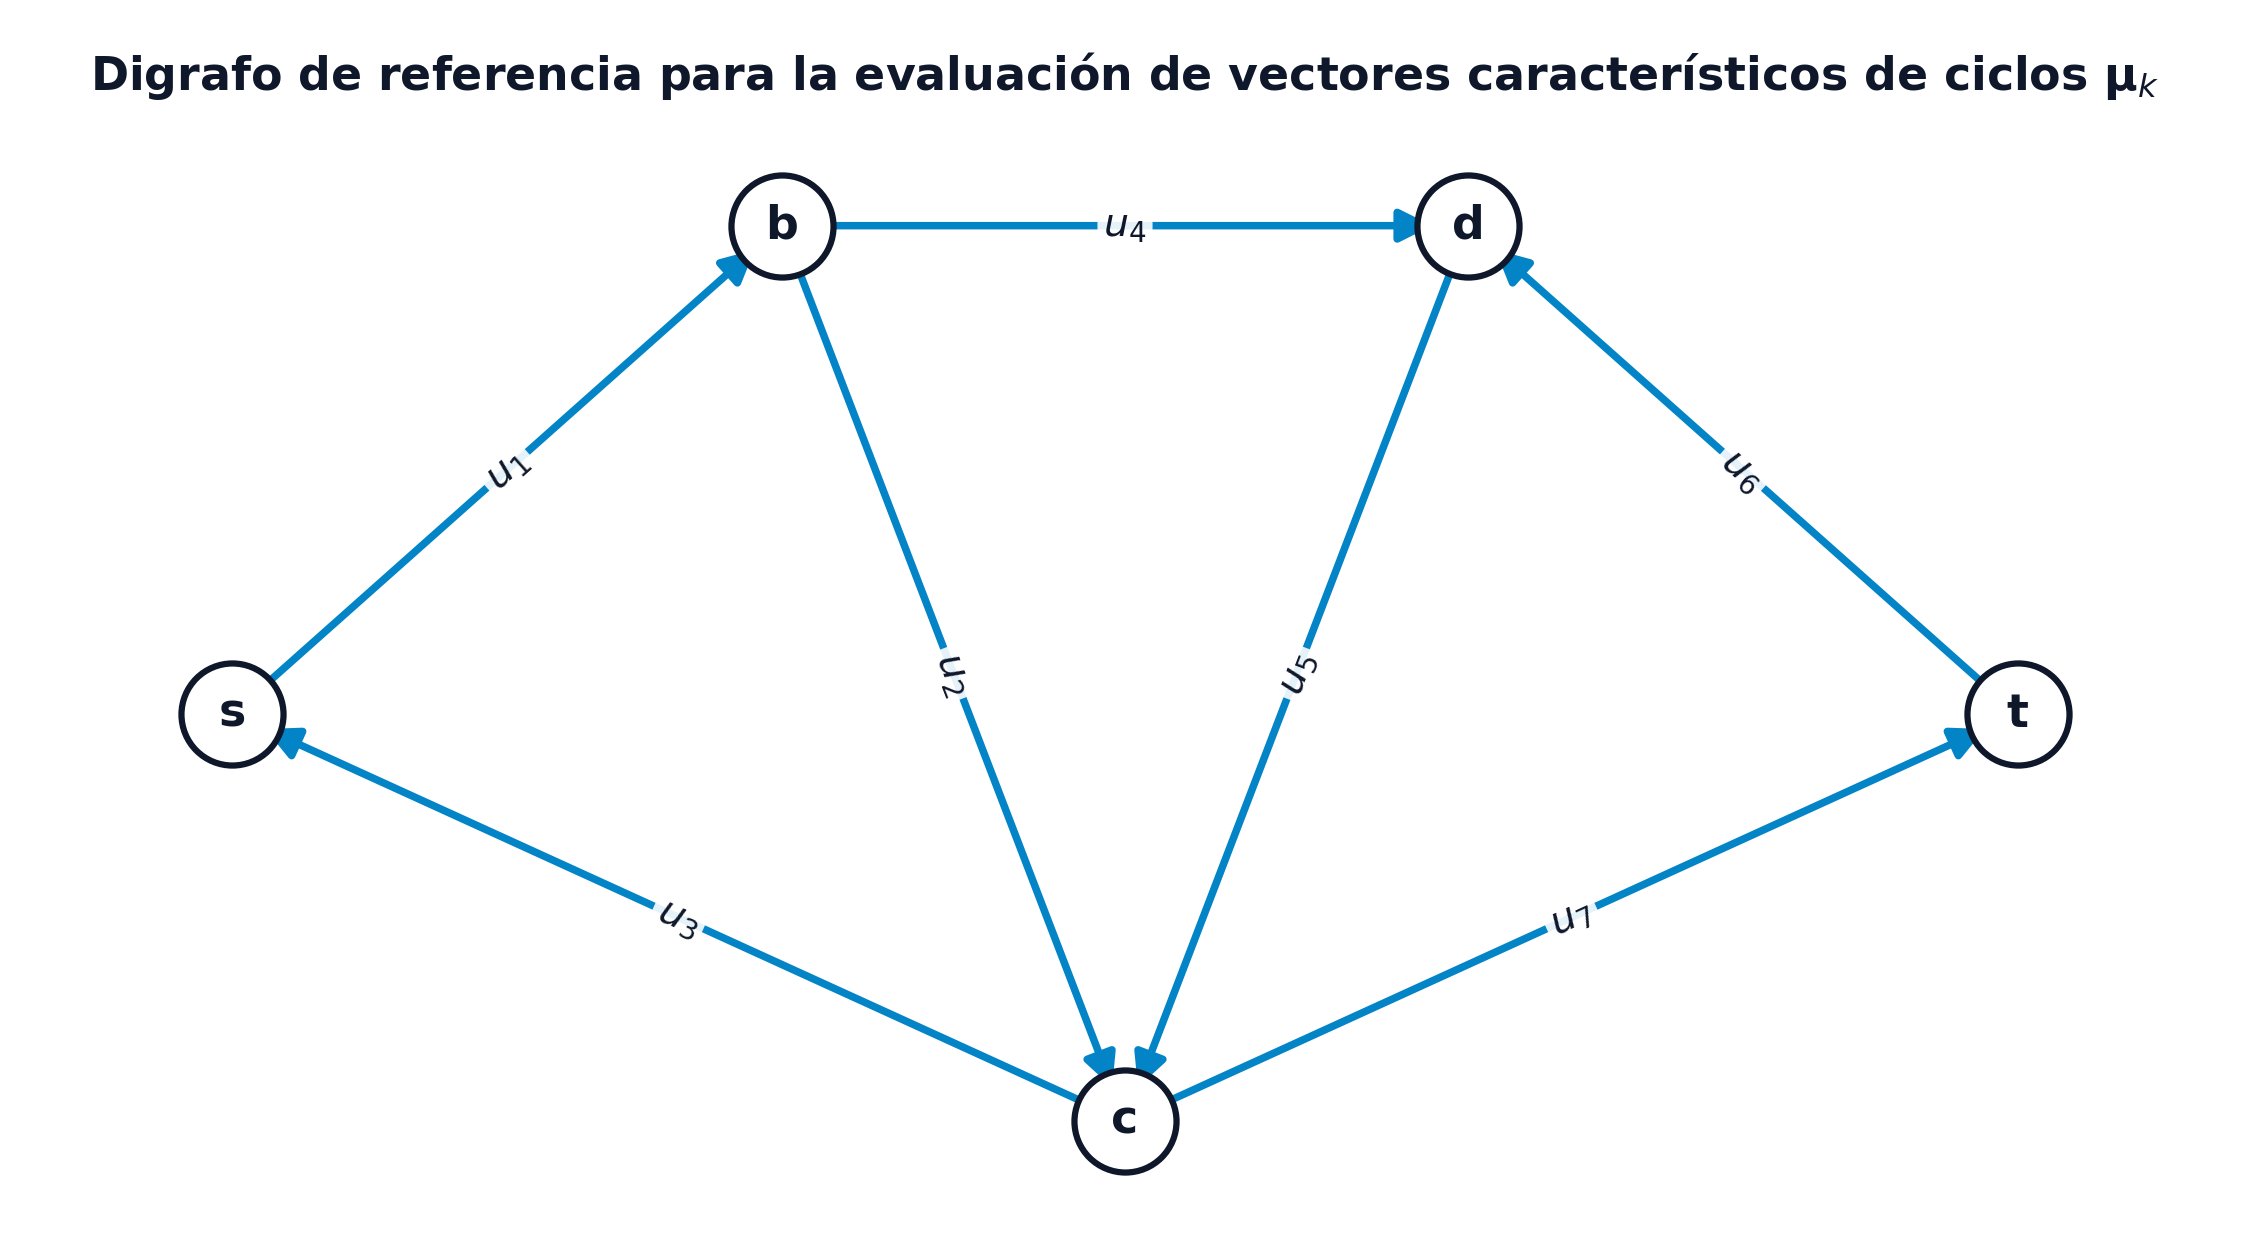
\includegraphics[width=0.65\linewidth,height=\textheight,keepaspectratio]{images/ciclos_vectores_ejemplo.png}

}

\caption{\label{fig-ciclos-vectores}Digrafo de referencia para la
evaluación de vectores característicos de ciclos}

\end{figure}%

Analizando las componentes de los vectores característicos, se
comprueban de forma inmediata las siguientes relaciones lineales entre
los ciclos:

\[
\mathbf{\mu}_1 = -\mathbf{\mu}_5, \qquad \mathbf{\mu}_3 = \mathbf{\mu}_1 + \mathbf{\mu}_2
\]

Esta propiedad demuestra que las combinaciones lineales de ciclos
generan nuevos vectores característicos de ciclos, lo que fundamenta la
estructura de espacio vectorial del conjunto de flujos.

\end{tcolorbox}

\begin{tcolorbox}[enhanced jigsaw, toprule=.15mm, opacitybacktitle=0.6, coltitle=black, colbacktitle=quarto-callout-note-color!10!white, title=\textcolor{quarto-callout-note-color}{\faInfo}\hspace{0.5em}{Proposición: Los ciclos son flujos}, arc=.35mm, rightrule=.15mm, toptitle=1mm, breakable, bottomtitle=1mm, titlerule=0mm, colback=white, opacityback=0, leftrule=.75mm, colframe=quarto-callout-note-color-frame, left=2mm, bottomrule=.15mm]

El vector característico \(\mathbf{\mu}\) asociado a cualquier ciclo en
un digrafo es un flujo.

\emph{Demostración}: Para cualquier nodo \(i \notin \mu\), ningún arco
incidente pertenece al ciclo, por lo que \(f_u = 0\) y la ley de
conservación se cumple de forma trivial (\(0 = 0\)). Para un nodo
\(i \in \mu\), el ciclo entra por un arco \(u_{in}\) y sale por otro
\(u_{out}\). Analizando la orientación de ambos arcos respecto al
sentido del giro (positivo o negativo), la contribución al balance
entrante \(\sum f_{in}\) y al balance saliente \(\sum f_{out}\) resulta
idéntica en ambos miembros, satisfaciéndose
\(\sum_{u \in w^+(i)} \mu_u = \sum_{u \in w^-(i)} \mu_u\).
\(\blacksquare\)

\end{tcolorbox}

Como se ilustra en la Figura~\ref{fig-ciclos-como-flujos}, los vectores
\(\mathbf{f}^2 = (0;\, 1;\, 1;\, 1;\, 0;\, 1;\, 0)^T\) y
\(\mathbf{f}^3 = (1;\, 0;\, -1;\, -1;\, 1;\, -1;\, -1)^T\) son flujos
válidos generados directamente por ciclos sobre la red de 5 nodos.

\begin{figure}

\centering{

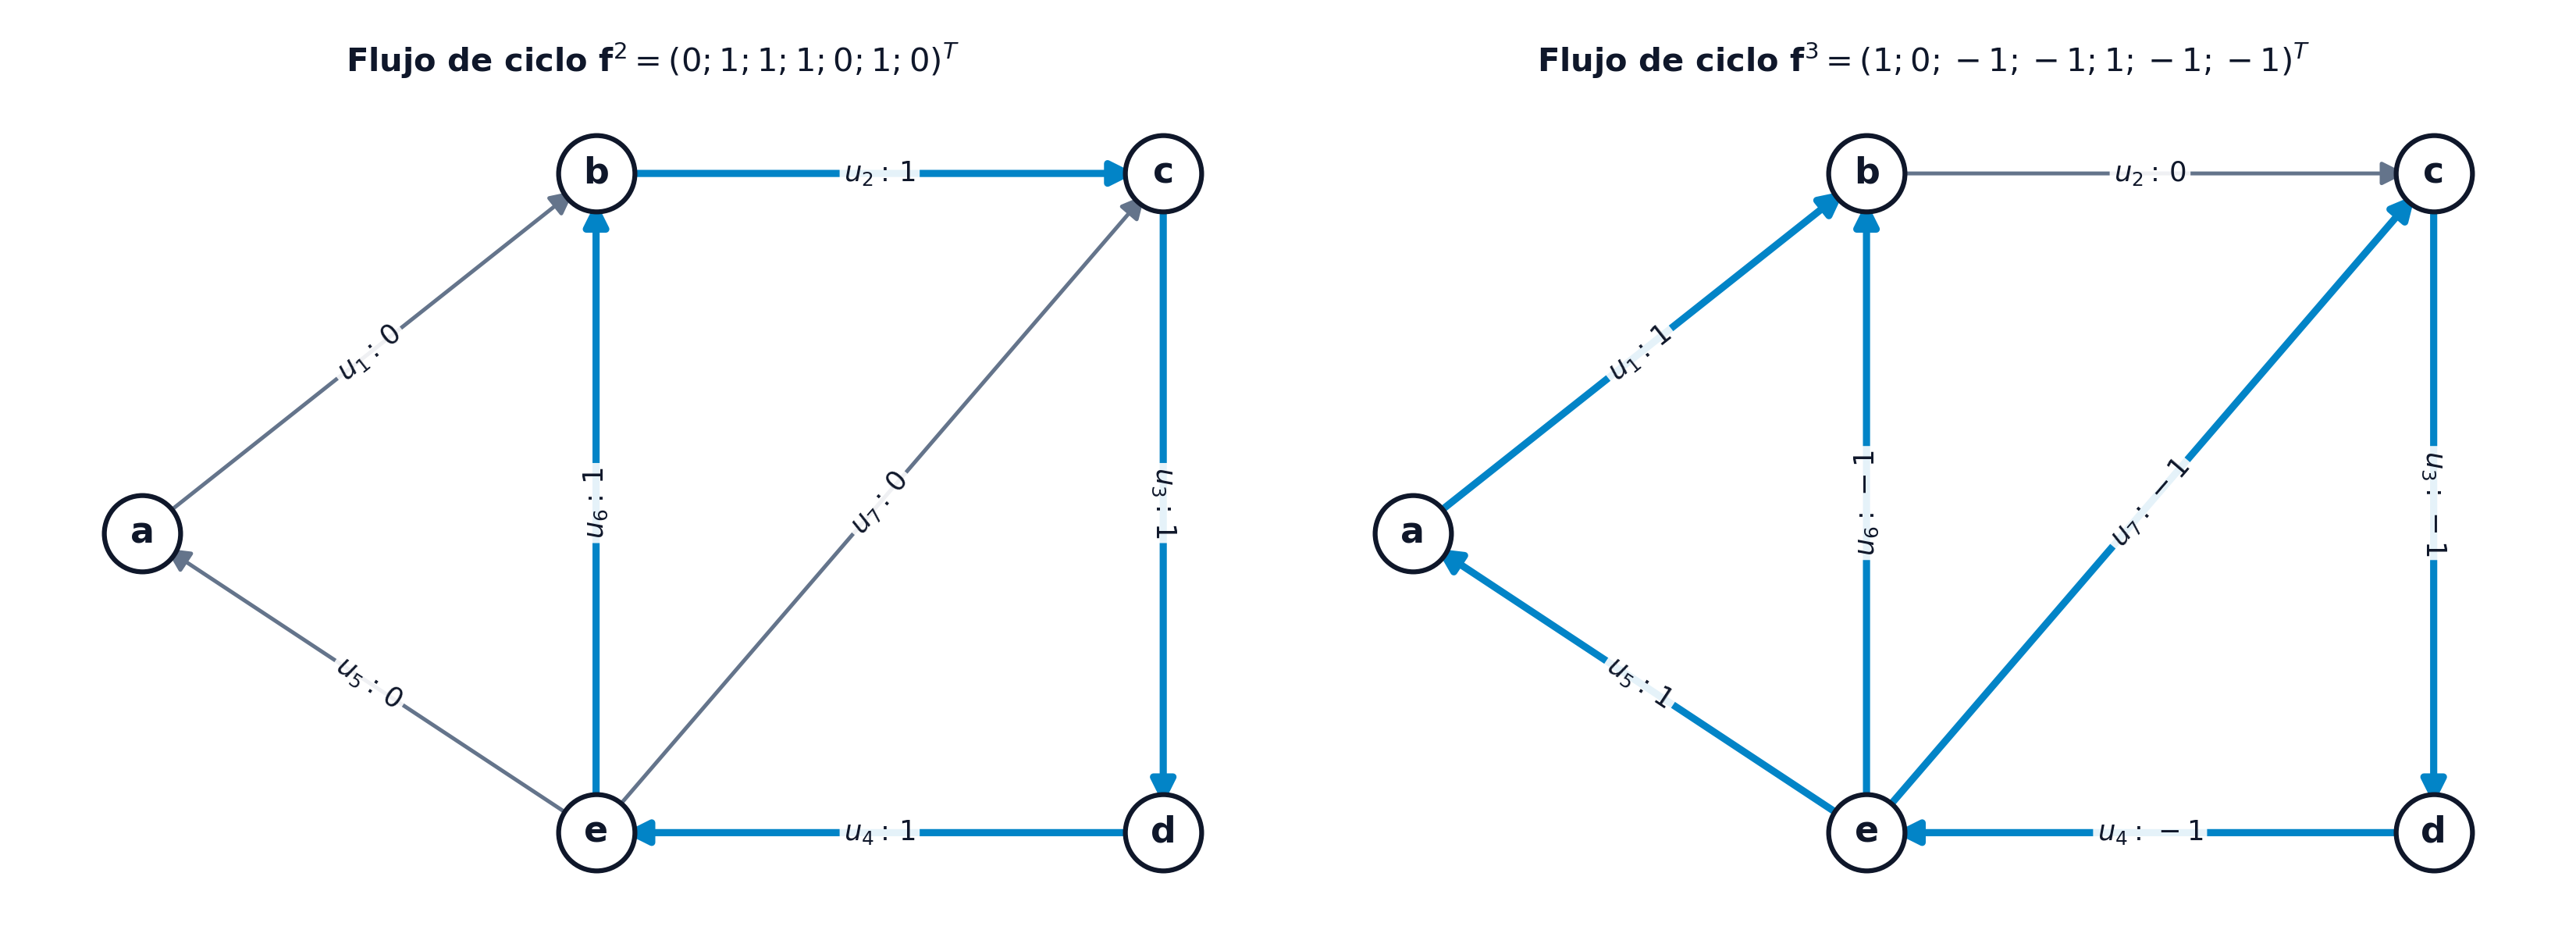
\includegraphics[width=0.85\linewidth,height=\textheight,keepaspectratio]{images/ciclos_como_flujos.png}

}

\caption{\label{fig-ciclos-como-flujos}Vectores de flujo
\(\mathbf{f}^2\) y \(\mathbf{f}^3\) generados por ciclos satisfaciendo
conservación en todos los nodos}

\end{figure}%

\begin{tcolorbox}[enhanced jigsaw, toprule=.15mm, opacitybacktitle=0.6, coltitle=black, colbacktitle=quarto-callout-note-color!10!white, title=\textcolor{quarto-callout-note-color}{\faInfo}\hspace{0.5em}{Corolario: Variación de flujo mediante ciclos}, arc=.35mm, rightrule=.15mm, toptitle=1mm, breakable, bottomtitle=1mm, titlerule=0mm, colback=white, opacityback=0, leftrule=.75mm, colframe=quarto-callout-note-color-frame, left=2mm, bottomrule=.15mm]

Dado un flujo \(\mathbf{f}\) en un digrafo \(G\) y un ciclo
\(\mathbf{\mu}\), el vector resultante de sumar a \(\mathbf{f}\) el
vector asociado al ciclo multiplicado por una constante
\(\alpha \in \mathbb{R}\)
(\(\mathbf{f}' = \mathbf{f} + \alpha \mathbf{\mu}\)) es también un flujo
en \(G\).

\end{tcolorbox}

\subsection{Bases de flujos y número
ciclomático}\label{bases-de-flujos-y-nuxfamero-ciclomuxe1tico}

Obviamente, no todos los flujos son ciclos. Sin embargo, cualquier flujo
se puede expresar como combinación lineal de ciclos. Además, es posible
identificar una base del espacio vectorial de los flujos de un digrafo.

Esta base está formada exclusivamente por ciclos y se obtiene a partir
de un árbol soporte del digrafo. Por tanto, cada árbol soporte da lugar
a una base distinta del espacio vectorial de flujos.

\begin{tcolorbox}[enhanced jigsaw, toprule=.15mm, opacitybacktitle=0.6, coltitle=black, colbacktitle=quarto-callout-note-color!10!white, title=\textcolor{quarto-callout-note-color}{\faInfo}\hspace{0.5em}{Definición: Independencia de flujos}, arc=.35mm, rightrule=.15mm, toptitle=1mm, breakable, bottomtitle=1mm, titlerule=0mm, colback=white, opacityback=0, leftrule=.75mm, colframe=quarto-callout-note-color-frame, left=2mm, bottomrule=.15mm]

Dado un digrafo \(G = (V, U)\), un conjunto de flujos
\(\{\mathbf{f}^1, \mathbf{f}^2, \dots, \mathbf{f}^k\}\) es linealmente
independiente si sus correspondientes vectores en \(\mathbb{R}^m\) son
linealmente independientes.

\end{tcolorbox}

La propiedad de independencia lineal garantiza que ninguno de los flujos
de la base pueda construirse combinando los restantes. Para seleccionar
una base de flujos de forma constructiva a partir de la topología del
digrafo, el procedimiento matemático estándar se apoya en la elección de
un \textbf{árbol soporte} de la red.

\begin{tcolorbox}[enhanced jigsaw, toprule=.15mm, opacitybacktitle=0.6, coltitle=black, colbacktitle=quarto-callout-important-color!10!white, title=\textcolor{quarto-callout-important-color}{\faExclamation}\hspace{0.5em}{Teorema: Base fundamental de ciclos}, arc=.35mm, rightrule=.15mm, toptitle=1mm, breakable, bottomtitle=1mm, titlerule=0mm, colback=white, opacityback=0, leftrule=.75mm, colframe=quarto-callout-important-color-frame, left=2mm, bottomrule=.15mm]

Sea \(G = (V, U)\) un digrafo conexo con \(n\) vértices y \(m\) arcos, y
sea \(H = (V, T)\) un árbol soporte de \(G\) (formado por \(n - 1\)
arcos).

Al añadir a \(T\) cualquier arco fuera del árbol
\(u \in U \setminus T\), se forma un único ciclo elemental \(\mu^u\) en
\(G\) tal que \(\mu^u_u = 1\). El conjunto de ciclos
\(H = \{\mu^u \mid u \in U \setminus T\}\) constituye una \textbf{base
del espacio vectorial de flujos} del digrafo \(G\).

\emph{Demostración}: Debemos probar que el conjunto de ciclos \(H\) es
linealmente independiente y generador:

\begin{enumerate}
\def\labelenumi{\arabic{enumi}.}
\tightlist
\item
  \textbf{Independencia lineal}: Cada arco fuera del árbol
  \(u \in U \setminus T\) pertenece a un único ciclo de la base (aquel
  generado por el propio arco \(u\)). Por tanto, la componente
  \(\mu^u_u = 1\) mientras que \(\mu^{u'}_u = 0\) para cualquier otro
  \(u' \in U \setminus T\). La matriz construida con los vectores de la
  base contiene una submatriz identidad de dimensión
  \(|U \setminus T| = m - n + 1\), lo que garantiza independencia
  lineal.
\item
  \textbf{Carácter generador}: Sea un flujo arbitrario
  \(\mathbf{f} = (f_1, \dots, f_m)^T\). Definimos el vector
  \(\mathbf{g} = \mathbf{f} - \sum_{u \in U \setminus T} f_u \mathbf{\mu}^u\).
  Como \(\mathbf{g}\) es combinación lineal de flujos, \(\mathbf{g}\) es
  un flujo. Para cualquier arco \(u \in U \setminus T\), la componente
  \(g_u = f_u - f_u (1) = 0\). Por tanto, el flujo \(\mathbf{g}\) tiene
  componentes nulas en todos los arcos de \(U \setminus T\). Esto
  implica que \(\mathbf{g}\) es un flujo definido únicamente sobre el
  árbol \(T\). Por el Lema de Flujo Nulo en Árboles, se deduce que
  \(\mathbf{g} = \mathbf{0}\), demostrando que
  \(\mathbf{f} = \sum_{u \in U \setminus T} f_u \mathbf{\mu}^u\).
  \(\blacksquare\)
\end{enumerate}

\end{tcolorbox}

El teorema anterior demuestra que el número de vectores necesarios para
generar cualquier circulación en el digrafo queda determinado
exclusivamente por la cantidad de arcos fuera del árbol soporte. Esta
dimensión algebraica se conoce como número ciclomático del grafo.

\begin{tcolorbox}[enhanced jigsaw, toprule=.15mm, opacitybacktitle=0.6, coltitle=black, colbacktitle=quarto-callout-note-color!10!white, title=\textcolor{quarto-callout-note-color}{\faInfo}\hspace{0.5em}{Definición: Número ciclomático}, arc=.35mm, rightrule=.15mm, toptitle=1mm, breakable, bottomtitle=1mm, titlerule=0mm, colback=white, opacityback=0, leftrule=.75mm, colframe=quarto-callout-note-color-frame, left=2mm, bottomrule=.15mm]

Se define el \textbf{número ciclomático} \(\nu(G)\) de un digrafo conexo
\(G = (V, U)\) como la dimensión del espacio vectorial de sus flujos:

\[
\nu(G) = m - n + 1
\]

\end{tcolorbox}

El número ciclomático \(\nu(G)\) nos indica que, independientemente de
cuán compleja sea la red, basta con identificar \(m - n + 1\) cuerdas no
básicas para caracterizar unívocamente todo el espacio de circulaciones.
A continuación, aplicamos este procedimiento constructivo sobre una red
concreta de 5 nodos y 7 arcos.

\begin{tcolorbox}[enhanced jigsaw, toprule=.15mm, opacitybacktitle=0.6, coltitle=black, colbacktitle=quarto-callout-tip-color!10!white, title=\textcolor{quarto-callout-tip-color}{\faLightbulb}\hspace{0.5em}{Ejemplo: Construcción de una base de ciclos y descomposición de un flujo}, arc=.35mm, rightrule=.15mm, toptitle=1mm, breakable, bottomtitle=1mm, titlerule=0mm, colback=white, opacityback=0, leftrule=.75mm, colframe=quarto-callout-tip-color-frame, left=2mm, bottomrule=.15mm]

Considérese el digrafo de \(n = 5\) nodos y \(m = 7\) arcos de la
\textbf{?@fig-base-ciclos-descomposicion-animado}. Su número ciclomático
es \(\nu(G) = m - n + 1 = 7 - 5 + 1 = 3\), lo que indica que el espacio
vectorial de flujos posee dimensión 3.

\textbf{Paso 1: Selección del Árbol Soporte y Cuerdas} Seleccionamos el
árbol soporte \(H = (V, T)\) formado por \(n - 1 = 4\) arcos:
\(T = \{u_1, u_4, u_5, u_7\}\) (representados en \textbf{azul}). Los 3
arcos fuera del árbol, denominados cuerdas o arcos no básicos, son
\(U \setminus T = \{u_2, u_3, u_6\}\) (representados en \textbf{gris}).

\textbf{Paso 2: Generación de la Base Fundamental de Ciclos} Al añadir
individualmente cada cuerda \(u \in U \setminus T\) al árbol soporte
\(T\), se forma exactamente un ciclo fundamental elemental
\(\mathbf{\mu}^u\) en el cual los arcos pertenecientes al ciclo se
destacan en \textbf{rojo}:

\begin{enumerate}
\def\labelenumi{\arabic{enumi}.}
\item
  \textbf{Añadir la cuerda \(u_2 = (b, c)\)}: Se cierra el ciclo
  \(b \to c \to e \to a \to b\). Fijando orientación positiva en \(u_2\)
  (\(\mu^2_{u_2} = 1\)), los arcos del árbol \(u_1, u_5\) avanzan en
  sentido directo y \(u_7\) en sentido opuesto, obteniéndose:
  \[ \mathbf{\mu}^2 = (1, 1, 0, 0, 1, 0, -1)^T \]
\item
  \textbf{Añadir la cuerda \(u_3 = (c, d)\)}: Se cierra el ciclo
  \(c \to d \to e \to c\). Con orientación positiva en \(u_3\)
  (\(\mu^3_{u_3} = 1\)), los arcos \(u_4, u_7\) avanzan en sentido
  directo, resultando: \[ \mathbf{\mu}^3 = (0, 0, 1, 1, 0, 0, 1)^T \]
\item
  \textbf{Añadir la cuerda \(u_6 = (e, b)\)}: Se cierra el ciclo
  \(e \to b \to a \to e\). Con orientación positiva en \(u_6\)
  (\(\mu^6_{u_6} = 1\)), los arcos \(u_1, u_5\) del árbol se recorren en
  sentido inverso, resultando:
  \[ \mathbf{\mu}^6 = (-1, 0, 0, 0, -1, 1, 0)^T \]
\end{enumerate}

El conjunto \(B = \{\mathbf{\mu}^2, \mathbf{\mu}^3, \mathbf{\mu}^6\}\)
es linealmente independiente y constituye una \textbf{base del espacio
vectorial de flujos}.

\textbf{Paso 3: Descomposición Unívoca de un Flujo en la Base} Dado el
flujo \(\mathbf{f} = (3, 4, 6, 6, 3, 1, 2)^T\), sus coordenadas de
descomposición en la base \(B\) vienen dadas de forma directa por los
valores del flujo en las cuerdas fuera del árbol: \(f_{u_2} = 4\),
\(f_{u_3} = 6\) y \(f_{u_6} = 1\). Se verifica la combinación lineal:

\[
\mathbf{f} = 4 \mathbf{\mu}^2 + 6 \mathbf{\mu}^3 + 1 \mathbf{\mu}^6 = 4 \begin{pmatrix} 1 \\ 1 \\ 0 \\ 0 \\ 1 \\ 0 \\ -1 \end{pmatrix} + 6 \begin{pmatrix} 0 \\ 0 \\ 1 \\ 1 \\ 0 \\ 0 \\ 1 \end{pmatrix} + 1 \begin{pmatrix} -1 \\ 0 \\ 0 \\ 0 \\ -1 \\ 1 \\ 0 \end{pmatrix} = \begin{pmatrix} 3 \\ 4 \\ 6 \\ 6 \\ 3 \\ 1 \\ 2 \end{pmatrix}
\]

\begin{figure}[H]

\centering{

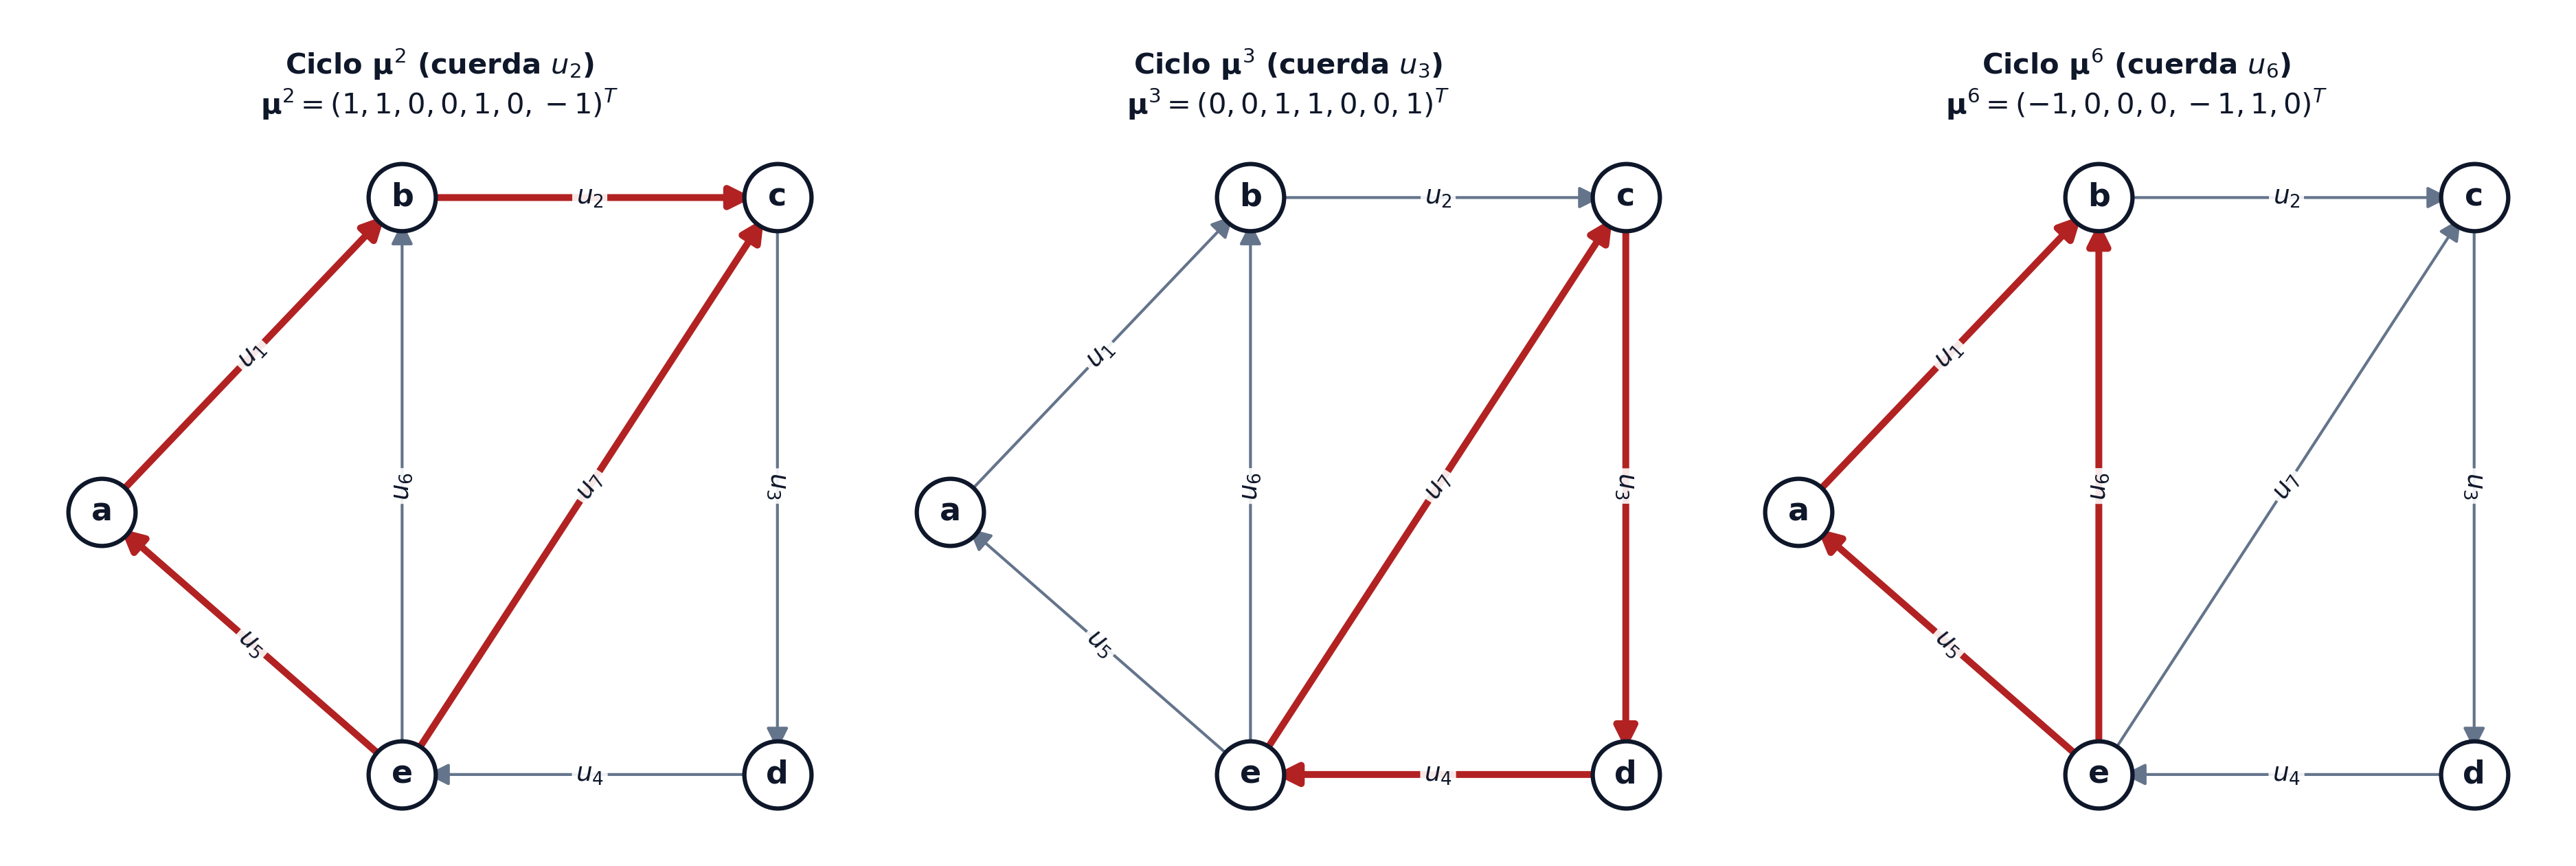
\includegraphics[width=0.85\linewidth,height=\textheight,keepaspectratio]{images/base_ciclos_tres_pasos.png}

}

\caption{\label{fig-base-ciclos-tres-pasos}Construcción paso a paso de
los tres ciclos fundamentales
\(\{\mathbf{\mu}^2, \mathbf{\mu}^3, \mathbf{\mu}^6\}\) de la base de
flujos}

\end{figure}%

\end{tcolorbox}

\subsection{Cociclos y Lema de Coloración de Arcos de
Minty}\label{cociclos-y-lema-de-coloraciuxf3n-de-arcos-de-minty}

Mientras que los ciclos representan circulaciones internas cerradas que
conservan el flujo localmente sin alterar los balances netos externos,
los \textbf{cociclos} (o cortes topológicos) representan la estructura
dual: barreras globales que separan el conjunto de vértices en dos
regiones disjuntas \(A\) y \(V \setminus A\). Los cociclos condicionan
la capacidad global de transporte de la red y determinan la existencia
de embotellamientos o cuellos de botella.

\begin{tcolorbox}[enhanced jigsaw, toprule=.15mm, opacitybacktitle=0.6, coltitle=black, colbacktitle=quarto-callout-note-color!10!white, title=\textcolor{quarto-callout-note-color}{\faInfo}\hspace{0.5em}{Definición: Cociclo (Corte)}, arc=.35mm, rightrule=.15mm, toptitle=1mm, breakable, bottomtitle=1mm, titlerule=0mm, colback=white, opacityback=0, leftrule=.75mm, colframe=quarto-callout-note-color-frame, left=2mm, bottomrule=.15mm]

Dado un digrafo conexo \(G = (V, U)\) y un subconjunto propio no vacío
de vértices \(A \subset V\), se define el \textbf{cociclo} \(w(A)\) como
el subconjunto de arcos que tienen un extremo en \(A\) y el otro en
\(V \setminus A\):

\[
w(A) = w^+(A) \cup w^-(A)
\]

donde:

\begin{itemize}
\tightlist
\item
  \textbf{Arcos salientes de \(A\)}:
  \(w^+(A) = \{ u = (i, j) \in U \mid i \in A, \, j \notin A \}\).
\item
  \textbf{Arcos entrantes a \(A\)}:
  \(w^-(A) = \{ u = (j, i) \in U \mid i \in A, \, j \notin A \}\).
\end{itemize}

\end{tcolorbox}

Para operar analíticamente con los cociclos e integrarlos en sistemas de
ecuaciones algebraicas, asignamos a cada cociclo un vector
característico que codifica la dirección del tránsito respecto a la
frontera de corte.

\begin{tcolorbox}[enhanced jigsaw, toprule=.15mm, opacitybacktitle=0.6, coltitle=black, colbacktitle=quarto-callout-note-color!10!white, title=\textcolor{quarto-callout-note-color}{\faInfo}\hspace{0.5em}{Definición: Vector característico de un cociclo}, arc=.35mm, rightrule=.15mm, toptitle=1mm, breakable, bottomtitle=1mm, titlerule=0mm, colback=white, opacityback=0, leftrule=.75mm, colframe=quarto-callout-note-color-frame, left=2mm, bottomrule=.15mm]

Un cociclo \(w(A)\) se representa algebraicamente mediante un vector
característico
\(\mathbf{\theta} = (\theta_1, \theta_2, \dots, \theta_m)^T \in \mathbb{R}^m\),
cuyas componentes se definen como:

\[
\theta_u = \begin{cases}
+1 & \text{si } u \in w^+(A) \\
-1 & \text{si } u \in w^-(A) \\
0 & \text{si } u \notin w(A)
\end{cases}
\]

\end{tcolorbox}

La distinción visual en los diagramas de corte resulta fundamental para
comprender la partición topológica: los vértices pertenecientes al
conjunto \(A\) se identifican mediante contorno y texto en \textbf{azul
cerúleo}, mientras que los vértices del complemento \(V \setminus A\)
permanecen en \textbf{slate oscuro}. Los arcos que cruzan la frontera
entre ambas particiones forman el cociclo \(w(A)\) y se destacan en
\textbf{rojo teja}, mientras que los arcos cuyos dos extremos pertenecen
a la misma partición (internos a \(A\) o internos a \(V \setminus A\))
permanecen en \textbf{gris slate}.

\begin{figure}

\centering{

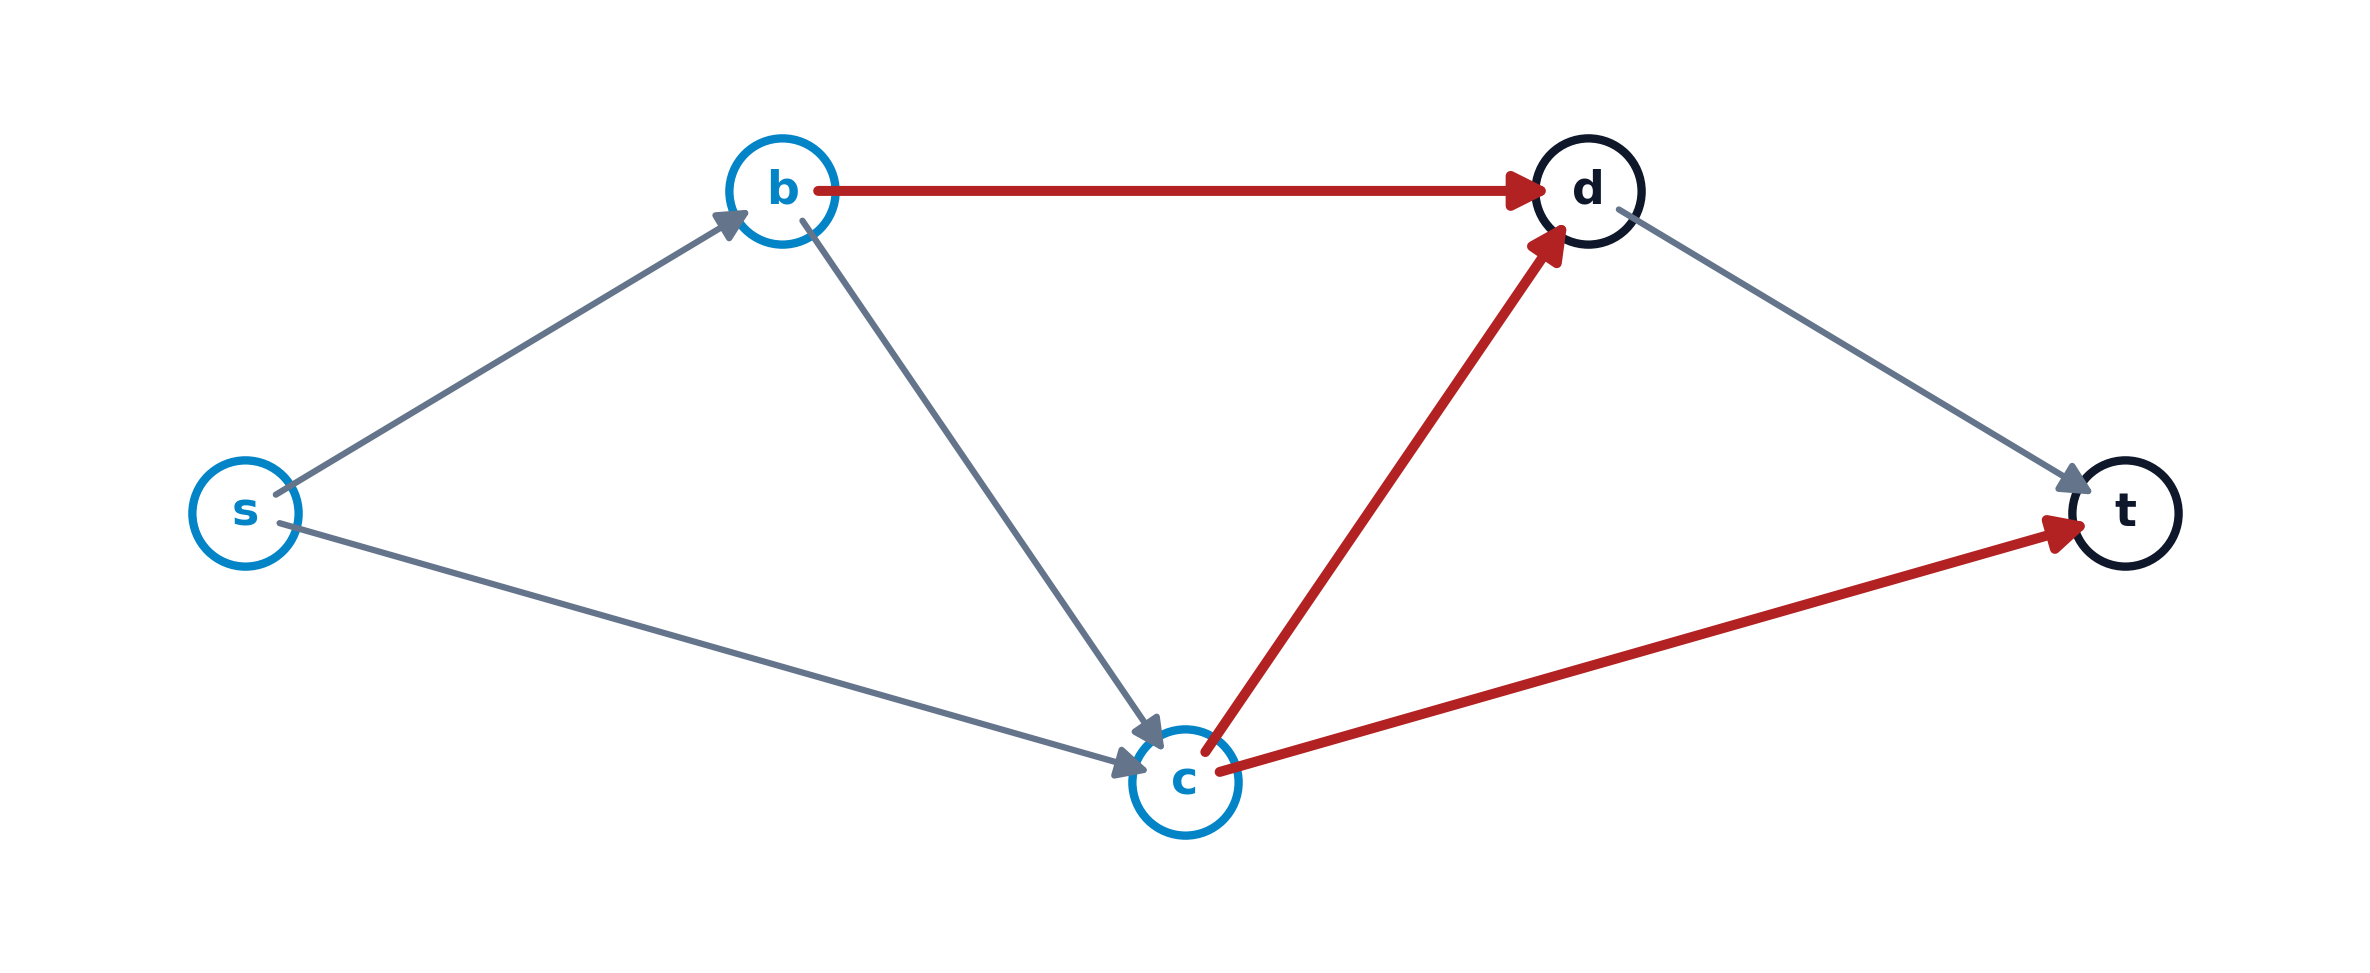
\includegraphics[width=0.65\linewidth,height=\textheight,keepaspectratio]{images/cociclo_corte_ejemplo.png}

}

\caption{\label{fig-cociclo-corte-ejemplo}Ilustración de un cociclo
\(w(A)\) separando el conjunto \(A=\{s, b, c\}\)}

\end{figure}%

Como se ilustra en la Figura~\ref{fig-cociclo-corte-ejemplo}, para el
subconjunto de nodos \(A = \{s, b, c\}\) (resaltados en azul), los arcos
que atraviesan la frontera hacia \(\{d, t\}\) son \(u_4 = (b, d)\),
\(u_5 = (d, c)\) y \(u_7 = (c, t)\), destacándose en \textbf{rojo teja}.
De ellos, \(u_4\) y \(u_7\) salen de \(A\) hacia el exterior
(\(w^+(A)\), asignándoles el valor \(+1\)), mientras que \(u_5\) entra
desde \(d \notin A\) hacia \(c \in A\) (\(w^-(A)\), asignándole el valor
\(-1\)). Los arcos \(u_1, u_2, u_3, u_6\) no cruzan la frontera y
reciben el valor \(0\), resultando el vector característico
\(\mathbf{\theta} = (0, 0, 0, 1, -1, 0, 1)^T\).

\begin{tcolorbox}[enhanced jigsaw, toprule=.15mm, opacitybacktitle=0.6, coltitle=black, colbacktitle=quarto-callout-tip-color!10!white, title=\textcolor{quarto-callout-tip-color}{\faLightbulb}\hspace{0.5em}{Ejemplo: Evaluación de vectores de cociclo en un digrafo}, arc=.35mm, rightrule=.15mm, toptitle=1mm, breakable, bottomtitle=1mm, titlerule=0mm, colback=white, opacityback=0, leftrule=.75mm, colframe=quarto-callout-tip-color-frame, left=2mm, bottomrule=.15mm]

Considérese el digrafo de \(n = 5\) nodos y \(m = 7\) arcos analizado
previamente. Para comprender cómo la elección del conjunto de vértices
\(A\) modifica radicalmente la frontera de corte y el vector
característico resultante, evaluamos dos particiones distintas \(A_1\) y
\(A_2\), ilustradas en la Figura~\ref{fig-cociclos-dos-ejemplos}:

\begin{enumerate}
\def\labelenumi{\arabic{enumi}.}
\item
  \textbf{Subconjunto \(A_1 = \{a, b, e\}\) (Subgráfico Izquierdo)}: En
  esta primera partición, los nodos \(a, b, e\) se encuentran en la
  región izquierda (destacados en \textbf{azul cerúleo}) y los nodos
  \(c, d\) en la región derecha (en \textbf{slate oscuro}). Analizamos
  los 7 arcos del digrafo uno a uno:

  \begin{itemize}
  \tightlist
  \item
    Arcos internos a \(A_1\): Los arcos \(u_1=(a,b)\), \(u_5=(e,a)\) y
    \(u_6=(e,b)\) conectan vértices que pertenecen ambos a \(A_1\). No
    cruzan la frontera y por tanto reciben el valor
    \(\theta_{u_1} = \theta_{u_5} = \theta_{u_6} = 0\).
  \item
    Arcos salientes de \(A_1\): El arco \(u_2=(b,c)\) parte de
    \(b \in A_1\) y llega a \(c \notin A_1\); de igual modo, el arco
    \(u_7=(e,c)\) parte de \(e \in A_1\) y llega a \(c \notin A_1\).
    Ambos son arcos directos o salientes: \(w^+(A_1) = \{u_2, u_7\}\),
    asignándoles el valor \(+1\)
    (\(\theta_{u_2} = 1, \theta_{u_7} = 1\)).
  \item
    Arcos entrantes a \(A_1\): El arco \(u_4=(d,e)\) parte de
    \(d \notin A_1\) e ingresa a \(e \in A_1\). Es un arco inverso o
    entrante: \(w^-(A_1) = \{u_4\}\), asignándole el valor \(-1\)
    (\(\theta_{u_4} = -1\)).
  \item
    Arcos externos a \(A_1\): El arco \(u_3=(c,d)\) conecta dos vértices
    fuera de \(A_1\), por lo que \(\theta_{u_3} = 0\).
  \item
    Vector característico de \(w(A_1)\):
    \(\mathbf{\theta}^1 = (0;\, 1;\, 0;\, -1;\, 0;\, 0;\, 1)^T\).
  \end{itemize}
\item
  \textbf{Subconjunto \(A_2 = \{b, d\}\) (Subgráfico Derecho)}: En esta
  segunda partición, los nodos \(b, d\) forman la región superior
  (destacados en \textbf{azul cerúleo}) y los nodos \(a, c, e\) forman
  la región inferior (en \textbf{slate oscuro}):

  \begin{itemize}
  \tightlist
  \item
    Arcos salientes de \(A_2\): Los arcos \(u_2=(b,c)\) (sale de
    \(b \in A_2\) hacia \(c\)) y \(u_4=(d,e)\) (sale de \(d \in A_2\)
    hacia \(e\)) cruzan la frontera hacia afuera:
    \(w^+(A_2) = \{u_2, u_4\}\), asignándoles el valor \(+1\)
    (\(\theta_{u_2} = 1, \theta_{u_4} = 1\)).
  \item
    Arcos entrantes a \(A_2\): Los arcos \(u_1=(a,b)\) (entra desde
    \(a\) a \(b \in A_2\)), \(u_3=(c,d)\) (entra desde \(c\) a
    \(d \in A_2\)) y \(u_6=(e,b)\) (entra desde \(e\) a \(b \in A_2\))
    cruzan la frontera hacia adentro: \(w^-(A_2) = \{u_1, u_3, u_6\}\),
    asignándoles el valor \(-1\)
    (\(\theta_{u_1} = -1, \theta_{u_3} = -1, \theta_{u_6} = -1\)).
  \item
    Arcos no incidentes en el corte: Los arcos \(u_5=(e,a)\) y
    \(u_7=(e,c)\) conectan nodos fuera de \(A_2\), por lo que
    \(\theta_{u_5} = \theta_{u_7} = 0\).
  \item
    Vector característico de \(w(A_2)\):
    \(\mathbf{\theta}^2 = (-1;\, 1;\, -1;\, 1;\, 0;\, -1;\, 0)^T\).
  \end{itemize}
\end{enumerate}

\begin{figure}[H]

\centering{

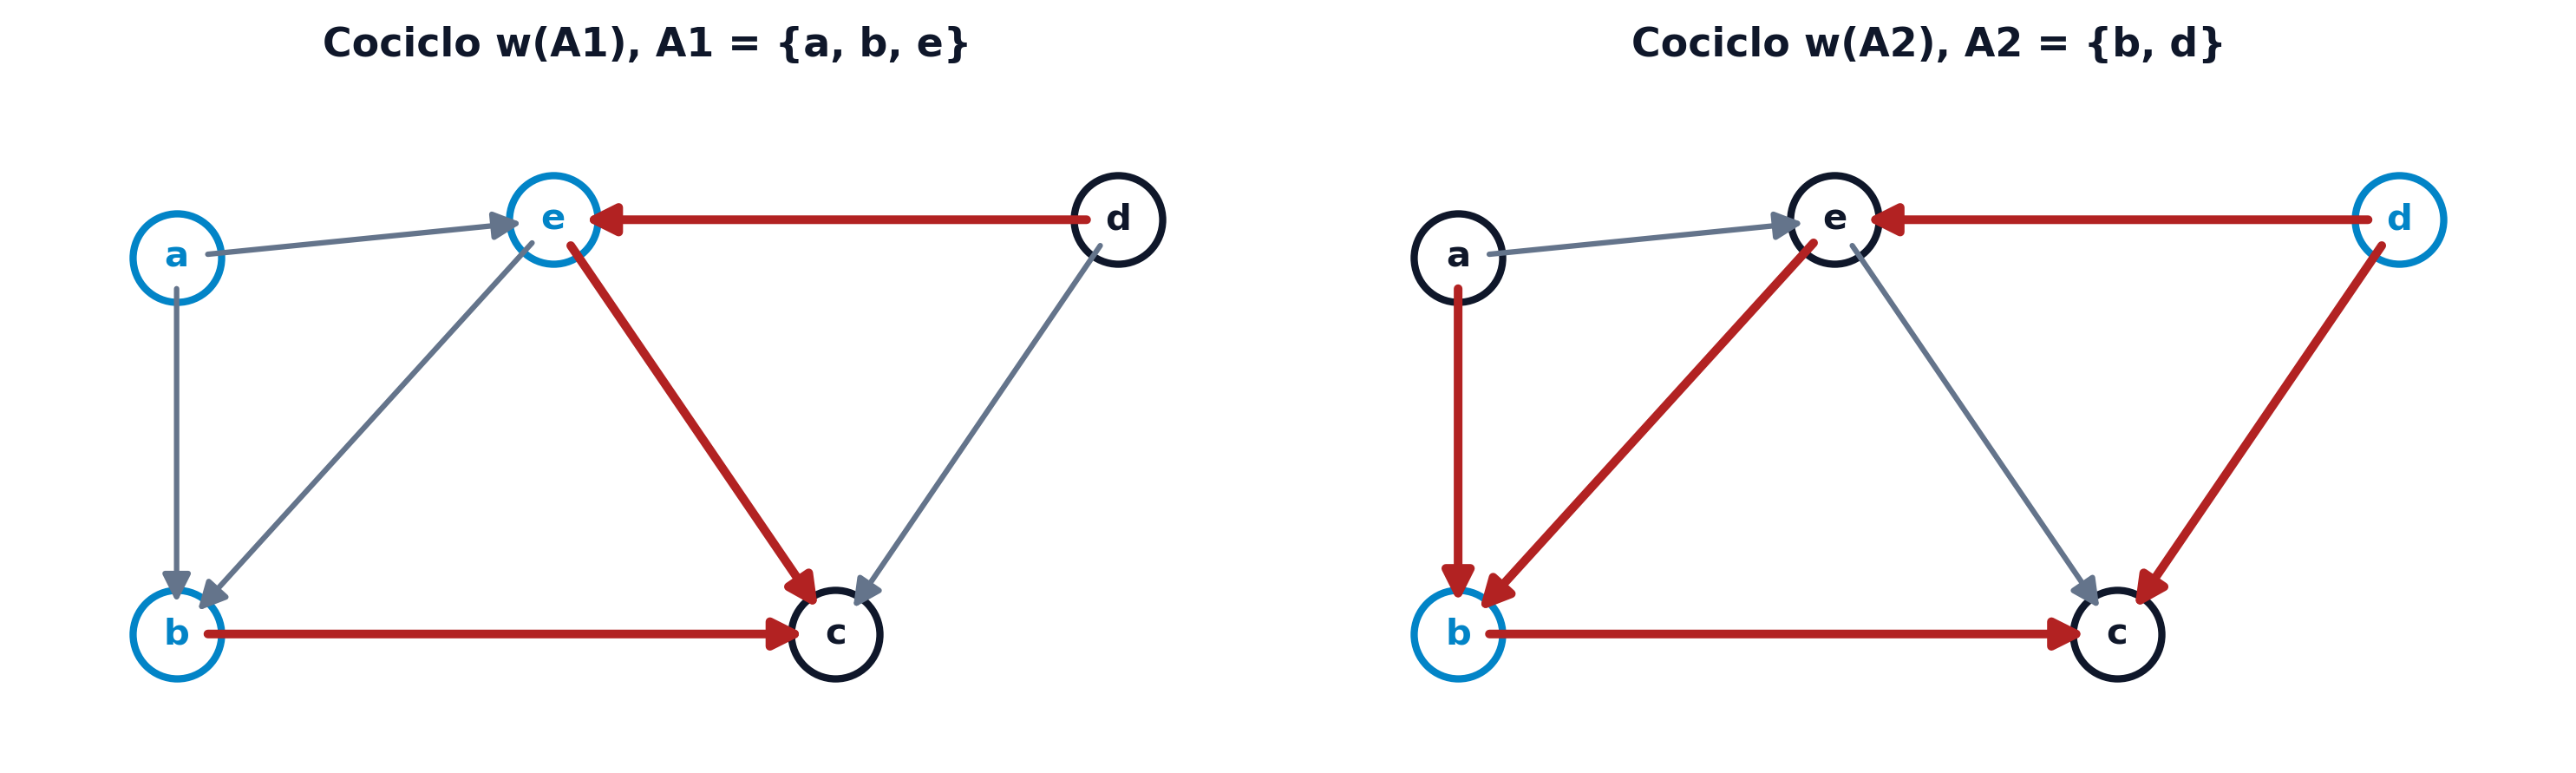
\includegraphics[width=0.95\linewidth,height=\textheight,keepaspectratio]{images/cociclos_dos_ejemplos.png}

}

\caption{\label{fig-cociclos-dos-ejemplos}Evaluación de los vectores de
cociclo \(\mathbf{\theta}^1\) y \(\mathbf{\theta}^2\) para los conjuntos
\(A_1 = \{a, b, e\}\) y \(A_2 = \{b, d\}\)}

\end{figure}%

\end{tcolorbox}

\subsection{Ortogonalidad fundamental entre ciclos y
cociclos}\label{ortogonalidad-fundamental-entre-ciclos-y-cociclos}

Existe una propiedad algebraica fundamental que vincula el espacio de
flujos (generado por los ciclos) con el espacio de cociclos (generado
por los cortes). Para cualquier ciclo \(\mathbf{\mu}\) y cualquier
cociclo \(\mathbf{\theta}\) definidos sobre el mismo digrafo
\(G = (V, U)\), su producto escalar es idénticamente nulo:

\[
\mathbf{\mu}^T \mathbf{\theta} = \sum_{u \in U} \mu_u \theta_u = 0
\]

Esta propiedad demuestra que el \textbf{espacio vectorial de flujos} (de
dimensión \(m - n + 1\)) y el \textbf{espacio vectorial de cociclos} (de
dimensión \(n - 1\)) son \textbf{subespacios ortogonales
complementarios} en \(\mathbb{R}^m\), satisfaciendo
\((m - n + 1) + (n - 1) = m\). Físicamente, esto significa que el caudal
neto transportado por cualquier circulación a través de un corte
topológico es exactamente igual a cero.

Una vez establecida la dualidad estricta entre el espacio de ciclos y el
espacio de cociclos, surge la pregunta de si es posible determinar cuál
de estas dos estructuras domina la conectividad de la red cuando los
arcos están sujetos a restricciones de orientación o estado.

Esta cuestión fue resuelta por George J. Minty en 1966 al formular el
\textbf{Lema de Coloración de Arcos}. El lema establece una dicotomía
matemática perfecta: al colorear arbitrariamente los arcos de un digrafo
conexo con tres colores (negro, verde y rojo) y fijar un arco negro de
referencia \(u_0\), \textbf{se verifica o bien la existencia de un ciclo
elemental coloreado que contiene a \(u_0\), o bien la existencia de un
cociclo elemental coloreado que contiene a \(u_0\), pero jamás ambos
simultáneamente}. Esta dicotomía constituye el motor lógico fundamental
para demostrar la convergencia del algoritmo de Ford-Fulkerson y el
Teorema Max-Flow Min-Cut.

\begin{tcolorbox}[enhanced jigsaw, toprule=.15mm, opacitybacktitle=0.6, coltitle=black, colbacktitle=quarto-callout-note-color!10!white, title=\textcolor{quarto-callout-note-color}{\faInfo}\hspace{0.5em}{Lema: Coloración de arcos de Minty}, arc=.35mm, rightrule=.15mm, toptitle=1mm, breakable, bottomtitle=1mm, titlerule=0mm, colback=white, opacityback=0, leftrule=.75mm, colframe=quarto-callout-note-color-frame, left=2mm, bottomrule=.15mm]

Sea \(G = (V, U)\) un digrafo conexo cuyos arcos se encuentran
coloreados (de forma arbitraria) utilizando tres colores: \textbf{negro}
(\(N\)), \textbf{verde} (\(V\)), \textbf{rojo} (\(R\)) o bien permanecen
\textbf{sin color} (\(0\)), existiendo al menos un arco de referencia
\(u_0 \in U\) coloreado de \textbf{negro}.

Entonces, se verifica \textbf{una, y solo una}, de las dos aseveraciones
siguientes:

\begin{enumerate}
\def\labelenumi{\arabic{enumi}.}
\tightlist
\item
  El arco negro \(u_0\) pertenece a un \textbf{ciclo elemental}
  coloreado (formado únicamente por arcos negros, verdes o rojos). En
  este ciclo, los arcos negros tienen orientación positiva, los arcos
  verdes tienen orientación negativa y los arcos rojos pueden tener
  cualquier orientación.
\item
  El arco negro \(u_0\) pertenece a un \textbf{cociclo elemental}
  coloreado (formado únicamente por arcos negros, verdes o sin color).
  En este cociclo, los arcos negros están en \(w^+(A)\) (mismo sentido
  que \(u_0\)), los verdes están en \(w^-(A)\) (sentido opuesto) y los
  arcos sin color pueden tener cualquier sentido.
\end{enumerate}

\emph{Demostración}: La demostración del lema es constructiva y se
fundamenta en un proceso sistemático de etiquetado de vértices.

Sea \(u_0 = (t, s)\) el arco de referencia coloreado de negro (origen en
\(t\) y destino en \(s\)).

\textbf{Paso 1: Etiquetado Inicial} Asignar una etiqueta al nodo destino
\(s\): \(p(s) = s\). El resto de vértices permanecen no etiquetados:
\(p(j) = 0, \forall j \neq s\).

\textbf{Paso 2: Propagación de Etiquetas} Repetir mientras sea posible
etiquetar nuevos vértices: dado un nodo \(i\) ya etiquetado
(\(p(i) \neq 0\)) y un nodo \(j\) no etiquetado (\(p(j) = 0\))
adyacentes en \(G\), asignar la etiqueta \(p(j) = i\) si se satisface
alguna de las siguientes reglas de color:

\begin{itemize}
\tightlist
\item
  Existe el arco dirigido \(u = (i, j) \in U\) (sale de \(i\) a \(j\)) y
  \(u\) está coloreado de \textbf{negro} o \textbf{rojo}.
\item
  Existe el arco dirigido \(u = (j, i) \in U\) (entra de \(j\) a \(i\))
  y \(u\) está coloreado de \textbf{verde} o \textbf{rojo}.
\end{itemize}

\textbf{Paso 3: Criterio de Parada y Análisis de Casos} Al finalizar el
proceso de etiquetado, se presenta una y solo una de las siguientes
situaciones:

\begin{itemize}
\item
  \textbf{Caso A (\(p(t) \neq 0\), el vértice \(t\) ha sido
  etiquetado)}: Reconstruyendo la cadena de antecedentes desde \(t\)
  hasta \(s\) (\(t - p(t) - p(p(t)) - \dots - s\)) y añadiendo el arco
  negro \(u_0 = (t, s)\), se obtiene un ciclo. Por la regla de
  etiquetado, todos sus arcos son negros, verdes o rojos. Los negros y
  rojos directos avanzan de \(i\) a \(j\) (orientación positiva),
  mientras que los verdes y rojos inversos van de \(j\) a \(i\)
  (orientación negativa). Esto satisface la \textbf{Afirmación 1}.
\item
  \textbf{Caso B (\(p(t) = 0\), el vértice \(t\) no pudo ser
  etiquetado)}: Definimos el conjunto de vértices etiquetados
  \(A = \{i \in V \mid p(i) \neq 0\}\). Como \(s \in A\) y
  \(t \notin A\), el arco negro \(u_0 = (t, s) \in w^-(A)\), o
  equivalentemente \(u_0 \in w^+(V \setminus A)\). Analizamos las
  propiedades del cociclo \(w(A)\):

  \begin{itemize}
  \tightlist
  \item
    No puede contener arcos \textbf{rojos}: si existiera un arco rojo
    \((i, j)\) con \(i \in A\) y \(j \notin A\), la regla del Paso 2
    habría etiquetado \(j\), contradiciendo que \(j \notin A\).
  \item
    Ningún arco \textbf{negro} puede pertenecer a \(w^-(A)\) (entrar a
    \(A\)): si existiera un arco negro \((j, i)\) con \(j \notin A\) e
    \(i \in A\), la segunda regla habría etiquetado \(j\).
  \item
    Ningún arco \textbf{verde} puede pertenecer a \(w^+(A)\) (salir de
    \(A\)): si existiera un arco verde \((i, j)\) con \(i \in A\) y
    \(j \notin A\), la segunda regla habría etiquetado \(j\).
  \end{itemize}

  En consecuencia, los arcos negros en \(w(A)\) son exclusivamente
  salientes (\(w^+(A)\)), los verdes son exclusivamente entrantes
  (\(w^-(A)\)) y los arcos sin color pueden tener cualquier sentido.
  Esto satisface la \textbf{Afirmación 2}. \(\blacksquare\)
\end{itemize}

\end{tcolorbox}

El procedimiento constructivo anterior demuestra que las tres reglas de
propagación de etiquetas garantizan siempre una dicotomía estricta. Para
visualizar de forma clara cómo el algoritmo busca la cadena de
antecedentes y cómo el color de cada arco determina la ruta de
etiquetado o la detención del proceso, consideremos la aplicación
completa del Lema sobre una red de 5 nodos en dos escenarios
alternativos de coloración.

\begin{tcolorbox}[enhanced jigsaw, toprule=.15mm, opacitybacktitle=0.6, coltitle=black, colbacktitle=quarto-callout-tip-color!10!white, title=\textcolor{quarto-callout-tip-color}{\faLightbulb}\hspace{0.5em}{Ejemplo: Aplicación del Lema de Coloración de Minty}, arc=.35mm, rightrule=.15mm, toptitle=1mm, breakable, bottomtitle=1mm, titlerule=0mm, colback=white, opacityback=0, leftrule=.75mm, colframe=quarto-callout-tip-color-frame, left=2mm, bottomrule=.15mm]

Considérese la red de 5 nodos \(V = \{a, b, c, d, e\}\) ilustrada en la
Figura~\ref{fig-minty-ejemplo-casos}, con arco negro de referencia
\(u_0 = (b, c)\). Se evalúan las dos coloraciones posibles para ilustrar
los dos casos alternativos del lema:

\begin{enumerate}
\def\labelenumi{\arabic{enumi}.}
\tightlist
\item
  \textbf{Caso A: Generación de un Ciclo (Gráfico Izquierdo)}

  \begin{itemize}
  \tightlist
  \item
    \textbf{Coloración asignada}: \(u_0 = (b,c)\) en \textbf{negro},
    \((e,b)\) en \textbf{rojo}, \((e,c), (d,c), (d,e), (a,e)\) en
    \textbf{verde}, y \((a,b)\) \textbf{sin color} (0).
  \item
    \textbf{Propagación del etiquetado}: Se inicia etiquetando el nodo
    destino del arco negro, \(p(c) = c\). A través del arco verde
    entrante \((e,c)\), se etiqueta \(p(e) = c\). A través del arco
    verde entrante \((d,c)\), se etiqueta \(p(d) = c\). Desde \(e\), a
    través del arco rojo saliente \((e,b)\), se etiqueta el nodo origen
    \(p(b) = e\).
  \item
    \textbf{Ciclo elemental resultante}: Al haber alcanzado el origen
    \(b\), se reconstruye la cadena \(b - e - c - b\), cerrando el ciclo
    \(\mu = \{(e,b), (e,c), (b,c)\}\) con arcos directos
    \(\mu^+ = \{(e,b), (b,c)\}\) y arco inverso \(\mu^- = \{(e,c)\}\).
  \end{itemize}
\item
  \textbf{Caso B: Generación de un Cociclo (Gráfico Derecho)}

  \begin{itemize}
  \tightlist
  \item
    \textbf{Coloración asignada}: \(u_0 = (b,c)\) en \textbf{negro},
    \((e,b), (e,c), (c,d)\) en \textbf{verde}, \((d,e), (a,b)\) en
    \textbf{negro}, y \((a,e)\) \textbf{sin color} (0).
  \item
    \textbf{Propagación del etiquetado}: Se inicia etiquetando
    \(p(c) = c\). A través del arco verde entrante \((e,c)\), se
    etiqueta \(p(e) = c\). Desde \(e\), el arco verde \((e,b)\) es
    saliente (no permite etiquetar \(b\)), el arco verde \((c,d)\) es
    saliente de \(c\) (no permite etiquetar \(d\)) y los arcos negros
    entrantes no están activos. El proceso se detiene sin etiquetar el
    origen \(b\) (\(p(b) = 0\)).
  \item
    \textbf{Cociclo elemental resultante}: El conjunto de nodos
    etiquetados es \(A = \{c, e\}\). El cociclo resultante \(w(A)\)
    presenta arcos salientes \(w^+(A) = \{(c,d), (e,b)\}\) y arcos
    entrantes \(w^-(A) = \{(b,c), (d,e), (a,e)\}\).
  \end{itemize}
\end{enumerate}

\begin{figure}[H]

\centering{

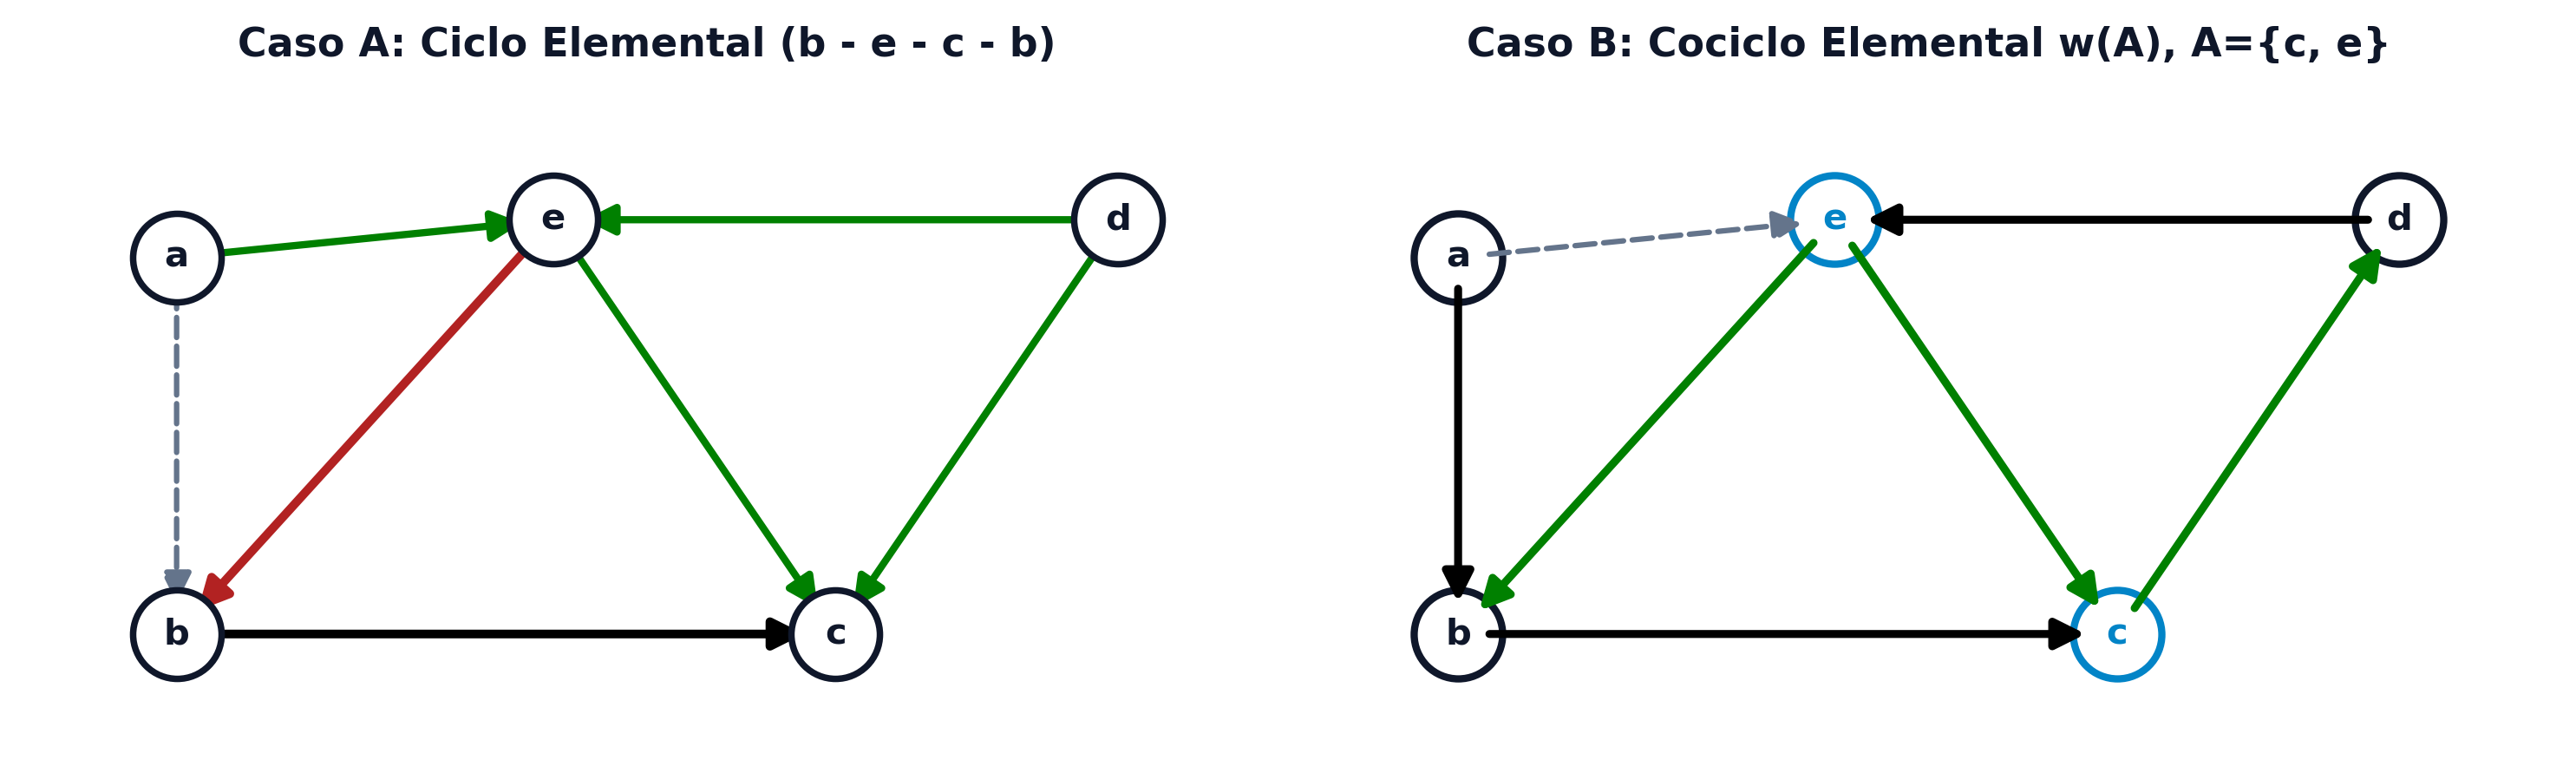
\includegraphics[width=0.95\linewidth,height=\textheight,keepaspectratio]{images/minty_ejemplo_casos.png}

}

\caption{\label{fig-minty-ejemplo-casos}Aplicación del algoritmo de
etiquetado del Lema de Minty: generación de un ciclo (izquierda) y
generación de un cociclo (derecha)}

\end{figure}%

\end{tcolorbox}

Una vez obtenido el ciclo o el cociclo mediante la ejecución del
algoritmo de etiquetado, resulta fundamental justificar formalmente por
qué la estructura geométrica resultante carece de redundancias o lazos
internos. El siguiente resultado complementario analiza la elementalidad
de las soluciones obtenidas por el método de Minty.

\begin{tcolorbox}[enhanced jigsaw, toprule=.15mm, opacitybacktitle=0.6, coltitle=black, colbacktitle=quarto-callout-note-color!10!white, title=\textcolor{quarto-callout-note-color}{\faInfo}\hspace{0.5em}{Observación: Elementalidad de los ciclos y cociclos de Minty}, arc=.35mm, rightrule=.15mm, toptitle=1mm, breakable, bottomtitle=1mm, titlerule=0mm, colback=white, opacityback=0, leftrule=.75mm, colframe=quarto-callout-note-color-frame, left=2mm, bottomrule=.15mm]

En la demostración constructiva del Lema de Minty se asume que las
estructuras algebraicas resultantes son elementales. Esta propiedad se
justifica formalmente mediante los siguientes argumentos:

\begin{enumerate}
\def\labelenumi{\arabic{enumi}.}
\item
  \textbf{Elementalidad del Ciclo}: Si la propagación de etiquetas
  alcanza el origen \(t\), el ciclo resultante es \textbf{necesariamente
  elemental}. La regla de asignación de antecesores \(p(j)\) asigna un
  único padre a cada nodo recién alcanzado, impidiendo que un mismo
  vértice sea etiquetado dos veces en la trayectoria de retorno de \(t\)
  a \(s\).
\item
  \textbf{Elementalidad del Cociclo}: Si la propagación se detiene sin
  alcanzar el origen \(t\), se obtiene la partición de vértices \(A\)
  (etiquetados) y \(V \setminus A\) (no etiquetados). Para que el
  cociclo \(w(A)\) sea \textbf{elemental}, los subgrafos inducidos
  \(G[A]\) y \(G[V \setminus A]\) deben ser conexos:

  \begin{itemize}
  \tightlist
  \item
    \textbf{Conexidad de \(G[A]\)}: Es conexo de forma trivial por la
    propia construcción del algoritmo, ya que cada vértice de \(A\) se
    añade siguiendo arcos adyacentes conectados con el nodo inicial
    \(s\).
  \item
    \textbf{Conexidad de \(G[V \setminus A]\)}: Supóngase por reducción
    al absurdo que el subgrafo \(G[V \setminus A]\) no fuera conexo y
    estuviera descompuesto en \(k \ge 2\) componentes conexas disjuntas:
    \[ V \setminus A = \bigcup_{h=1}^k B_h, \qquad B_h \cap B_{h'} = \emptyset, \; \forall h \neq h' \]
    Como el vértice \(t\) no pertenece a \(A\), debe estar contenido en
    una de dichas componentes (por ejemplo, \(t \in B_1\)). Consideremos
    la unión del conjunto \(A\) con el resto de componentes no
    conectadas con \(t\): \(A' = A \cup \bigcup_{h=2}^k B_h\). El
    cociclo \(w(A')\) generado por \(A'\) satisface las mismas
    propiedades de restricción de color que \(w(A)\) y además cumple que
    \((t, s) \in w^-(A') \subset w^-(A)\). Sin embargo, si
    \(G[V \setminus A]\) no fuera conexo, se contradiría la conexidad
    global del digrafo inicial \(G\), concluyendo que
    \(G[V \setminus A]\) es conexo y por tanto el cociclo \(w(A)\) es
    \textbf{elemental}.
  \end{itemize}
\end{enumerate}

\end{tcolorbox}

\section{El problema del flujo
máximo}\label{el-problema-del-flujo-muxe1ximo}

Un problema de flujo que surge de forma natural en la práctica es
obtener la máxima cantidad de flujo que se puede mover entre dos
vértices específicos de un digrafo. Es el denominado \textbf{problema
del flujo máximo}.

En este problema, cada arco del digrafo posee una capacidad limitada (la
cantidad máxima de caudal o flujo que puede transitar físicamente por él
por unidad de tiempo). Esto nos lleva a introducir el concepto de
\textbf{red de transporte}, que valora cada arco por la capacidad de
flujo que puede soportar.

\subsection{Redes de transporte y flujos
compatibles}\label{redes-de-transporte-y-flujos-compatibles}

Para estudiar formalmente el problema del flujo máximo, es preciso dotar
al digrafo de una estructura cuantitativa que limite el volumen de
tráfico que cada conexión puede albergar.

\begin{tcolorbox}[enhanced jigsaw, toprule=.15mm, opacitybacktitle=0.6, coltitle=black, colbacktitle=quarto-callout-note-color!10!white, title=\textcolor{quarto-callout-note-color}{\faInfo}\hspace{0.5em}{Definición: Red de transporte}, arc=.35mm, rightrule=.15mm, toptitle=1mm, breakable, bottomtitle=1mm, titlerule=0mm, colback=white, opacityback=0, leftrule=.75mm, colframe=quarto-callout-note-color-frame, left=2mm, bottomrule=.15mm]

Una \textbf{red de transporte} es un par \((G = (V, U), \mathbf{c})\),
donde \(G = (V, U)\) es un digrafo conexo sin bucles y
\(\mathbf{c} = \{c_u \mid u \in U\}\) representa el conjunto de
\textbf{capacidades} superiores no negativas asociadas a cada arco
\(u \in U\) (\(c_u \ge 0\)).

\end{tcolorbox}

Sobre una red de transporte, un vector de flujo es aceptable solo si no
excede los límites físicos de las infraestructuras de la red y satisface
la conservación local.

\begin{tcolorbox}[enhanced jigsaw, toprule=.15mm, opacitybacktitle=0.6, coltitle=black, colbacktitle=quarto-callout-note-color!10!white, title=\textcolor{quarto-callout-note-color}{\faInfo}\hspace{0.5em}{Definición: Flujo compatible (versión preliminar)}, arc=.35mm, rightrule=.15mm, toptitle=1mm, breakable, bottomtitle=1mm, titlerule=0mm, colback=white, opacityback=0, leftrule=.75mm, colframe=quarto-callout-note-color-frame, left=2mm, bottomrule=.15mm]

Dada una red de transporte \((G, \mathbf{c})\), se define un
\textbf{flujo compatible} como un vector
\(\mathbf{f} = (f_1, f_2, \dots, f_m)^T \in \mathbb{R}^m\) que
satisface:

\begin{enumerate}
\def\labelenumi{\arabic{enumi}.}
\item
  \textbf{Ley de conservación pura de flujo}:
  \[ \sum_{u \in w^+(i)} f_u - \sum_{u \in w^-(i)} f_u = 0, \quad \forall i \in V \]
\item
  \textbf{Compatibilidad con las capacidades}:
  \[ 0 \le f_u \le c_u, \quad \forall u \in U \]
\end{enumerate}

\end{tcolorbox}

Existe una paradoja sutil al aplicar la definición de conservación pura
a la transmisión de flujo entre un par de vértices fijados \(s\)
(fuente) y \(t\) (sumidero). En la inmensa mayoría de redes de
transporte práctico, de la fuente \(s\) solo salen arcos
(\(w^-(s) = \emptyset\)) y al sumidero \(t\) solo llegan arcos
(\(w^+(t) = \emptyset\)).

Si exigimos la conservación pura
\(\sum_{u \in w^+(i)} f_u = \sum_{u \in w^-(i)} f_u\) de forma estricta
en \textbf{todos} los nodos sin excepción:

\begin{itemize}
\tightlist
\item
  En el nodo fuente \(s\): como no entra ningún arco
  (\(\sum f_{ent} = 0\)), la suma de salientes debe ser cero
  (\(\sum f_{sal} = 0\)). Como \(f_u \ge 0\), se fuerza a que
  \(f_u = 0\) en todos los arcos salientes de \(s\).
\item
  En el nodo sumidero \(t\): como no sale ningún arco
  (\(\sum f_{sal} = 0\)), la suma de entrantes debe ser cero
  (\(\sum f_{ent} = 0\)).
\end{itemize}

Como se ilustra en la Figura~\ref{fig-red-conservacion-nula}, la
conservación estricta en \(s\) y \(t\) fuerza a que el \textbf{único
flujo compatible posible sea el flujo trivial nulo}
(\(\mathbf{f} = \mathbf{0}\)), impidiendo enviar cualquier caudal útil
desde la fuente hasta el destino.

\begin{figure}

\centering{

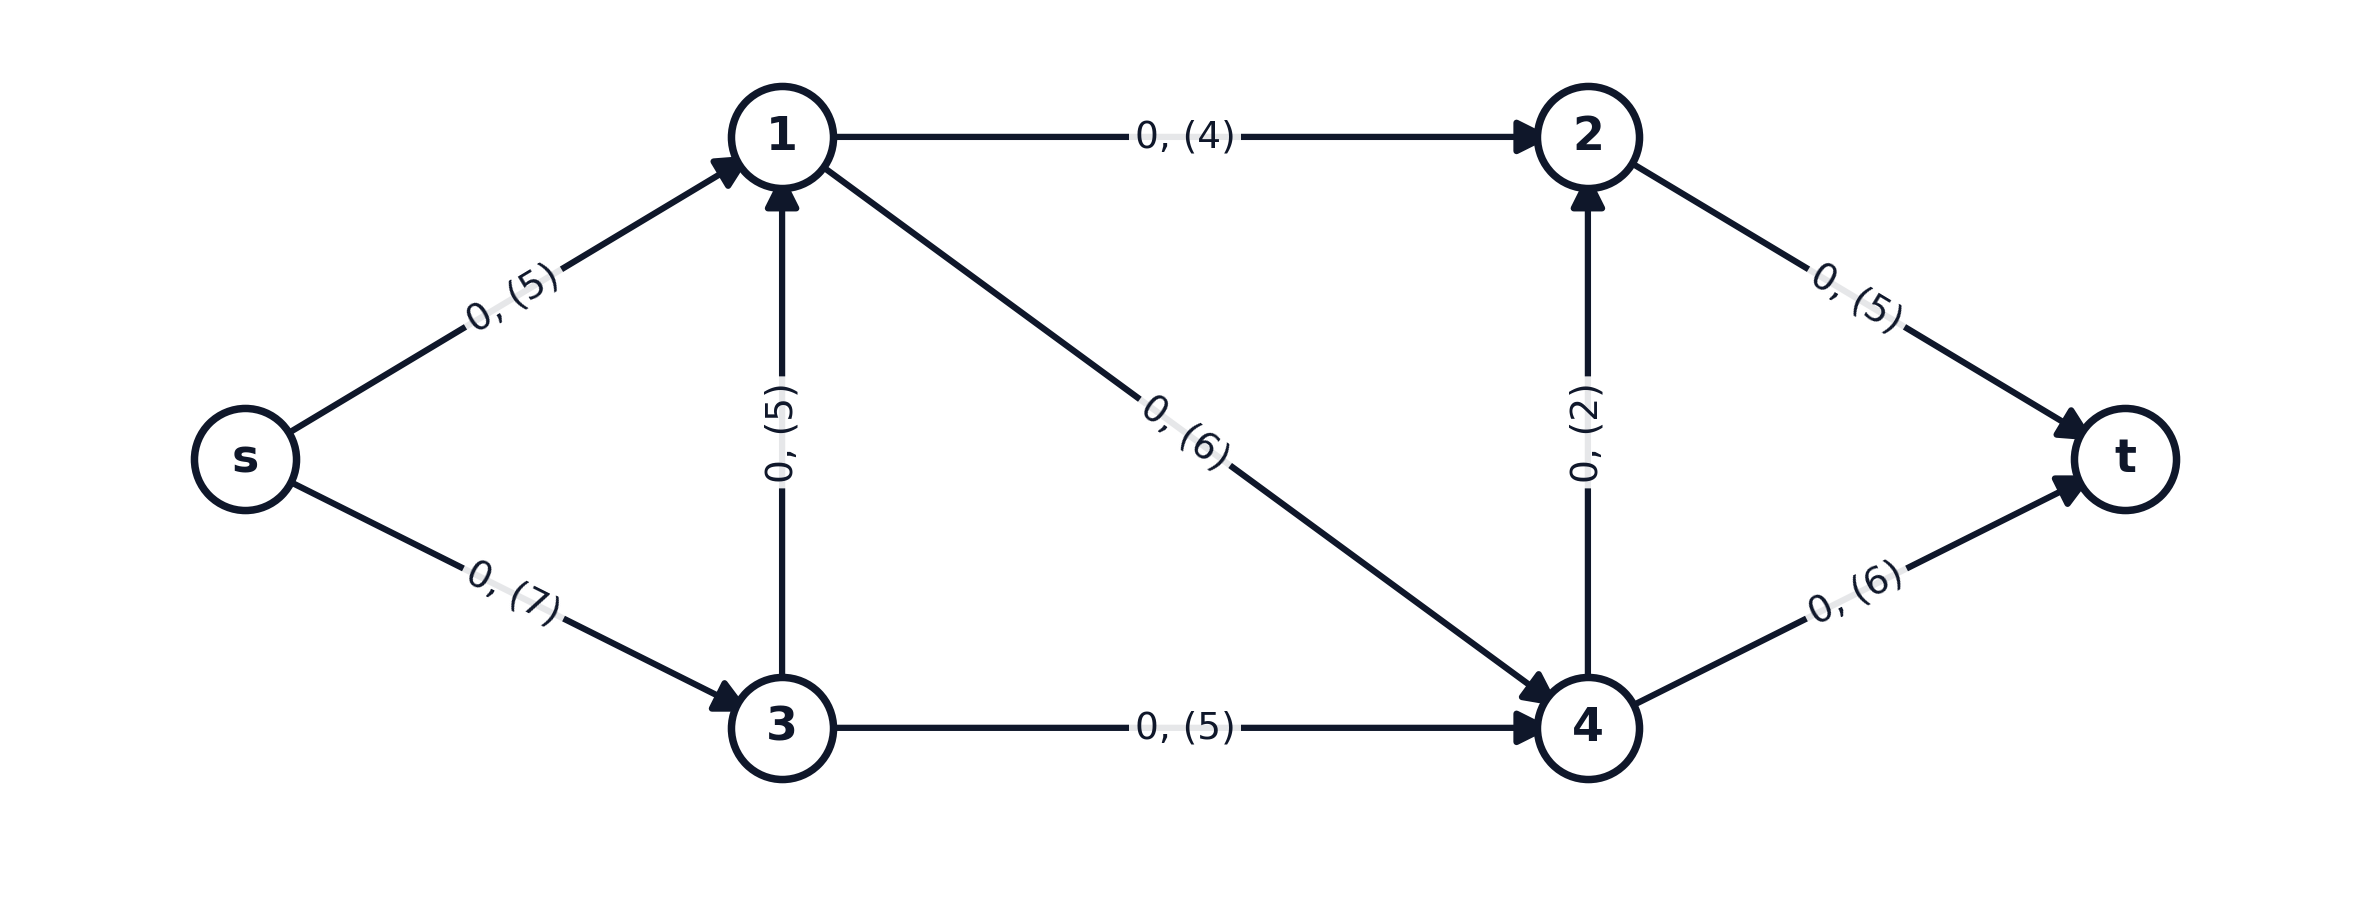
\includegraphics[width=0.75\linewidth,height=\textheight,keepaspectratio]{images/red_conservacion_nula.png}

}

\caption{\label{fig-red-conservacion-nula}Red de transporte donde la
exigencia de conservación pura en \(s\) y \(t\) fuerza el flujo nulo
trivial \(\mathbf{f} = \mathbf{0}\)}

\end{figure}%

Para solventar este dilema matemático sin romper la estructura de
espacio vectorial de las circulaciones ni tener que tratar a \(s\) y
\(t\) como excepciones algorítmicas, se introduce una construcción muy
elegante: el \textbf{arco ficticio de retorno \(u_0 = (t, s)\)}.

Conectamos el sumidero \(t\) de regreso a la fuente \(s\) mediante un
arco ficticio \(u_0 = (t, s)\) dotado de \textbf{capacidad ilimitada}
(\(c_0 = \infty\)). De este modo, todo el flujo que llega a \(t\)
``recircula'' de vuelta a \(s\) a través de \(u_0\), cerrando la red en
una verdadera \textbf{circulación}.

\begin{figure}

\centering{

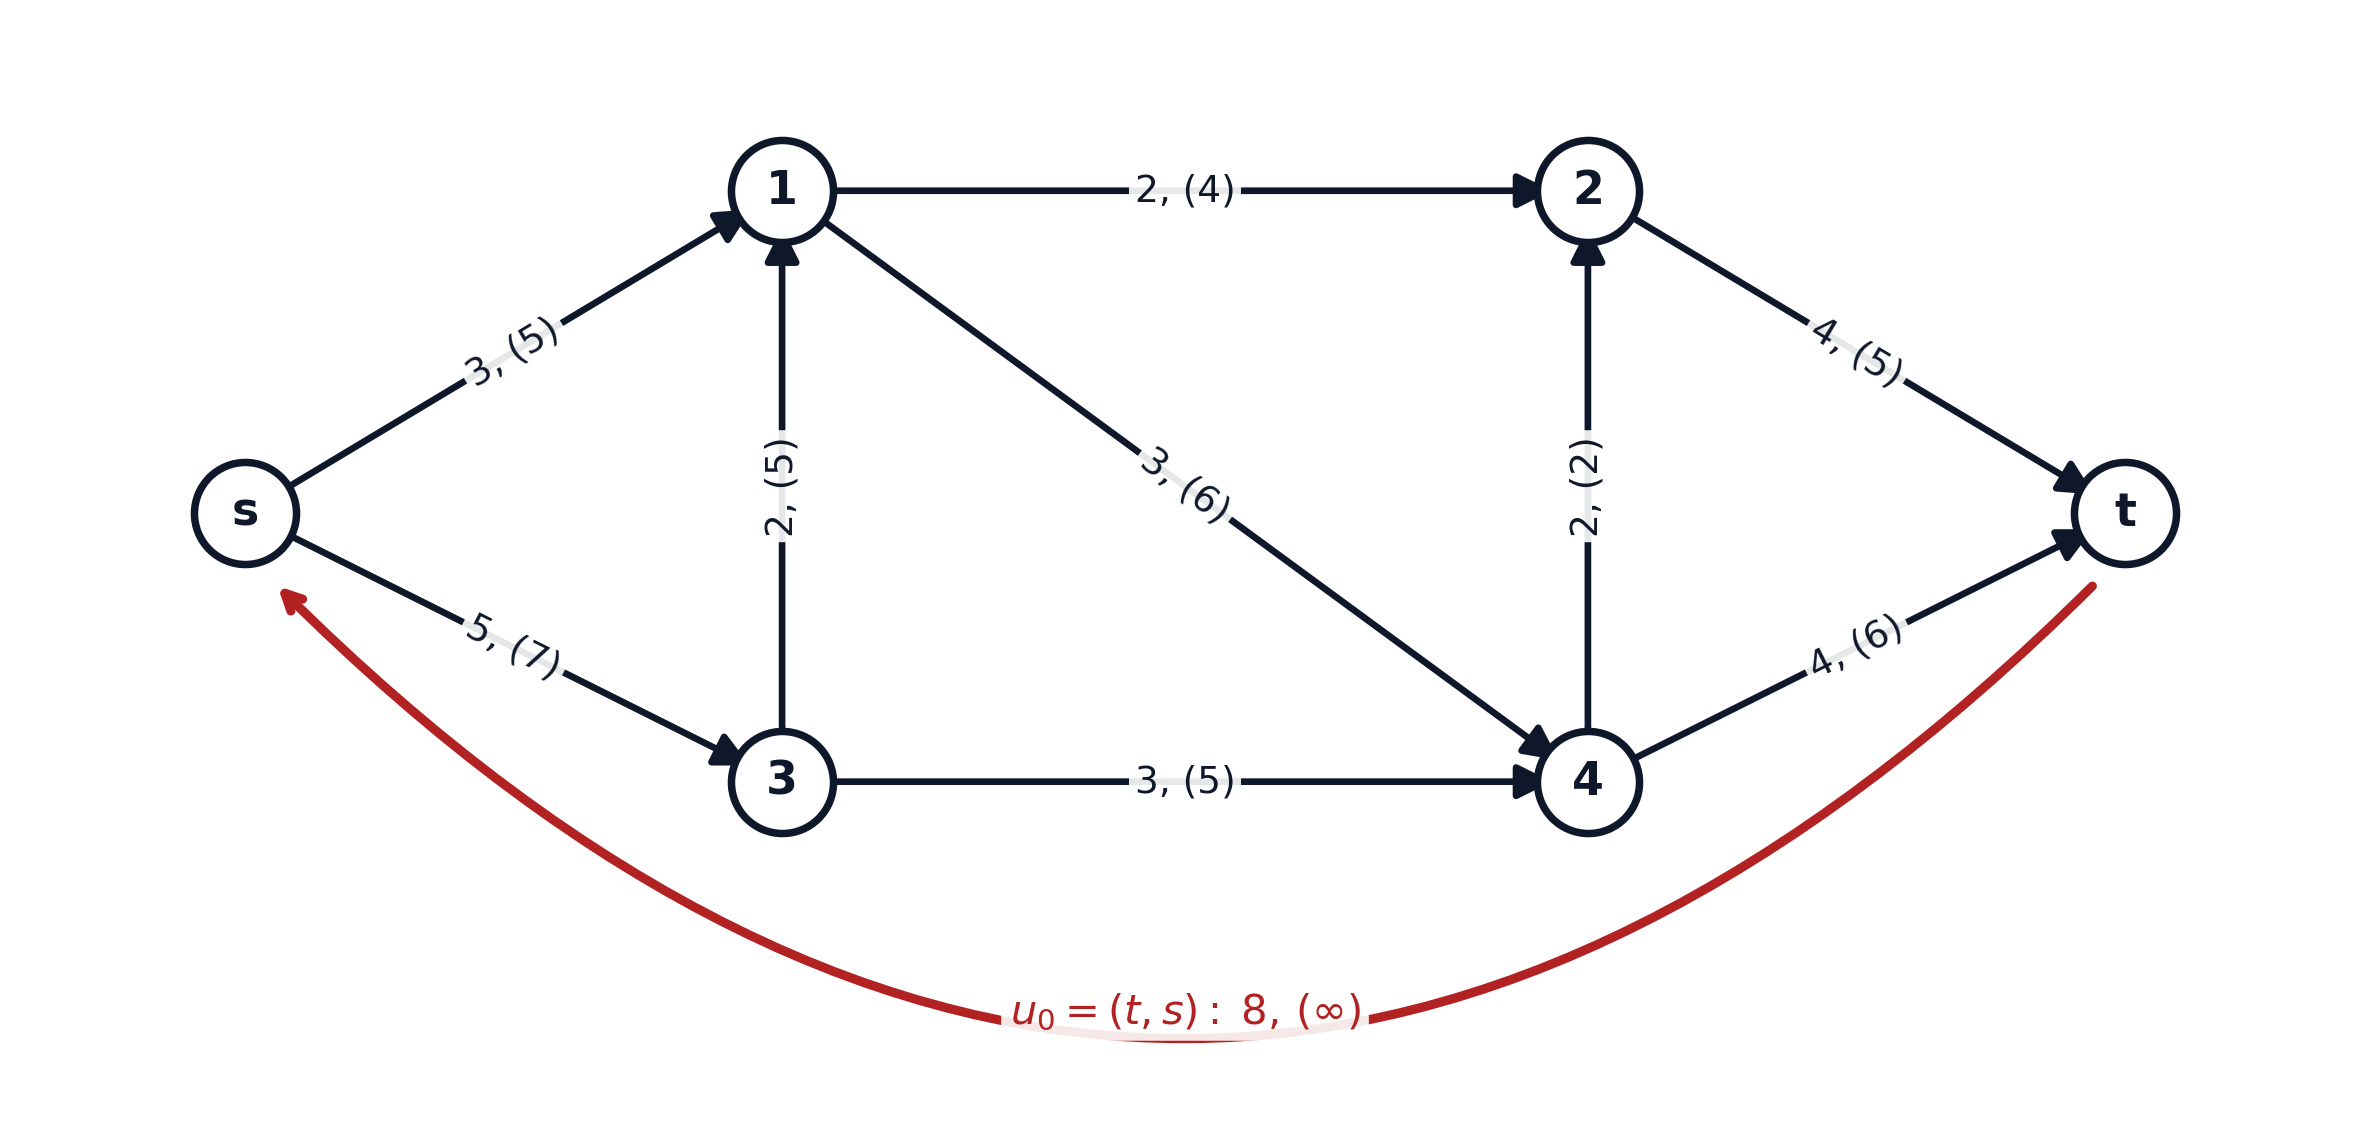
\includegraphics[width=0.8\linewidth,height=\textheight,keepaspectratio]{images/red_flujo_compatible_retorno.png}

}

\caption{\label{fig-red-flujo-compatible-retorno}Red de transporte
ampliada con el arco ficticio de retorno \(u_0 = (t, s)\) llevando un
valor de flujo \(f_0 = 8\)}

\end{figure}%

Como se ilustra en la Figura~\ref{fig-red-flujo-compatible-retorno}, el
flujo \(f_0 = f_{(t, s)}\) que circula por el arco ficticio de retorno
representa de forma directa el \textbf{valor del flujo total}
\(v(\mathbf{f})\) transmitido por la red desde \(s\) hasta \(t\):

\[
f_0 = v(\mathbf{f}) = \sum_{j \in \Gamma^+(s)} f_{sj} = \sum_{j \in \Gamma^-(t)} f_{jt}
\]

\begin{tcolorbox}[enhanced jigsaw, toprule=.15mm, opacitybacktitle=0.6, coltitle=black, colbacktitle=quarto-callout-note-color!10!white, title=\textcolor{quarto-callout-note-color}{\faInfo}\hspace{0.5em}{Definición formal: \((s, t)\)-Flujo compatible}, arc=.35mm, rightrule=.15mm, toptitle=1mm, breakable, bottomtitle=1mm, titlerule=0mm, colback=white, opacityback=0, leftrule=.75mm, colframe=quarto-callout-note-color-frame, left=2mm, bottomrule=.15mm]

Dada una red de transporte \((G = (V, U), \mathbf{c})\) y dos vértices
fijados \(s, t \in V\), se define un \textbf{\((s, t)\)-flujo
compatible} como una circulación factible sobre la red ampliada
\(G' = (V, U \cup \{u_0=(t,s)\})\) con \(c_0 = \infty\), satisfaciendo
\(0 \le f_u \le c_u, \, \forall u \in U\).

\end{tcolorbox}

Una vez caracterizadas las redes de transporte y los \((s, t)\)-flujos
compatibles con el arco ficticio de retorno \(u_0 = (t, s)\), podemos
formular de manera rigurosa el problema del flujo máximo.

\begin{tcolorbox}[enhanced jigsaw, toprule=.15mm, opacitybacktitle=0.6, coltitle=black, colbacktitle=quarto-callout-note-color!10!white, title=\textcolor{quarto-callout-note-color}{\faInfo}\hspace{0.5em}{Definición: Problema del flujo máximo}, arc=.35mm, rightrule=.15mm, toptitle=1mm, breakable, bottomtitle=1mm, titlerule=0mm, colback=white, opacityback=0, leftrule=.75mm, colframe=quarto-callout-note-color-frame, left=2mm, bottomrule=.15mm]

Dada una red de transporte \((G = (V, U), \mathbf{c})\) y fijados dos
vértices \(s, t \in V\) (fuente y sumidero), el \textbf{problema del
flujo máximo} consiste en determinar un \((s, t)\)-flujo compatible
\(\mathbf{f}^* \in \mathbb{R}^m\) tal que el valor del flujo \(f_0\) que
circula por el arco ficticio de retorno \(u_0 = (t, s)\) sea máximo.

Algebraicamente, el problema se formula como:

\[
\begin{aligned}
\max_{\mathbf{f} \in \mathbb{R}^m} \quad & f_0 = \sum_{j \in \Gamma^+(s)} f_{sj} = \sum_{j \in \Gamma^-(t)} f_{jt} \\
\text{s.a.} \quad & \sum_{u \in w^+(i)} f_u - \sum_{u \in w^-(i)} f_u = 0, \quad \forall i \in V \\
& 0 \le f_u \le c_u, \quad \forall u \in U
\end{aligned}
\]

\end{tcolorbox}

El \textbf{valor del flujo} \(f_0\) representa cuantitativamente la
cantidad total de caudal que sale de la fuente \(s\) y llega
efectivamente al sumidero \(t\).

\begin{tcolorbox}[enhanced jigsaw, toprule=.15mm, opacitybacktitle=0.6, coltitle=black, colbacktitle=quarto-callout-tip-color!10!white, title=\textcolor{quarto-callout-tip-color}{\faLightbulb}\hspace{0.5em}{Ejemplo: Evaluación de compatibilidad y saturación por capacidad}, arc=.35mm, rightrule=.15mm, toptitle=1mm, breakable, bottomtitle=1mm, titlerule=0mm, colback=white, opacityback=0, leftrule=.75mm, colframe=quarto-callout-tip-color-frame, left=2mm, bottomrule=.15mm]

Considérese la red de transporte de 6 nodos \(V = \{s, b, c, d, e, t\}\)
ilustrada en la Figura~\ref{fig-red-flujo-saturacion-ejemplo}, equipada
con el arco de retorno ficticio \(u_0 = (t, s)\) llevando un flujo
circulante de \(f_0 = 8\) unidades (\(v(\mathbf{f}) = 8\)).

Evaluamos las condiciones de compatibilidad en los arcos de la red:

\begin{enumerate}
\def\labelenumi{\arabic{enumi}.}
\tightlist
\item
  \textbf{Flujo compatible base}: En el estado ilustrado, todos los
  arcos satisfacen \(0 \le f_u \le c_u\). Por ejemplo, el arco
  \((s, b)\) transita con \(f_{sb} = 5 \le c_{sb} = 5\) (arco saturado),
  mientras que \((b, c)\) transita con \(f_{bc} = 2 \le c_{bc} = 3\) (no
  saturado).
\item
  \textbf{Evaluación de una modificación por ciclo}: Supóngase que
  intentamos incrementar el flujo enviando 2 unidades adicionales a lo
  largo del circuito cerrado \(c \to d \to e \to c\) (destacado en
  \textbf{rojo teja} en la figura).

  \begin{itemize}
  \tightlist
  \item
    En el arco \((c, d)\), el flujo aumentaría de \(f_{cd} = 1\) a
    \(1 + 2 = 3\). Sin embargo, su capacidad es \(c_{cd} = 1\), por lo
    que \(3 > 1\) violando la restricción de capacidad.
  \item
    De igual modo, en \((d, e)\) el flujo pasaría a
    \(4 + 2 = 6 > c_{de} = 3\), e \((e, c)\) pasaría a
    \(2 + 2 = 4 > c_{ec} = 1\).
  \end{itemize}
\end{enumerate}

\emph{Conclusión}: La adición de dicho ciclo destruye la compatibilidad
del flujo al exceder las capacidades límite de los arcos.

\begin{figure}[H]

\centering{

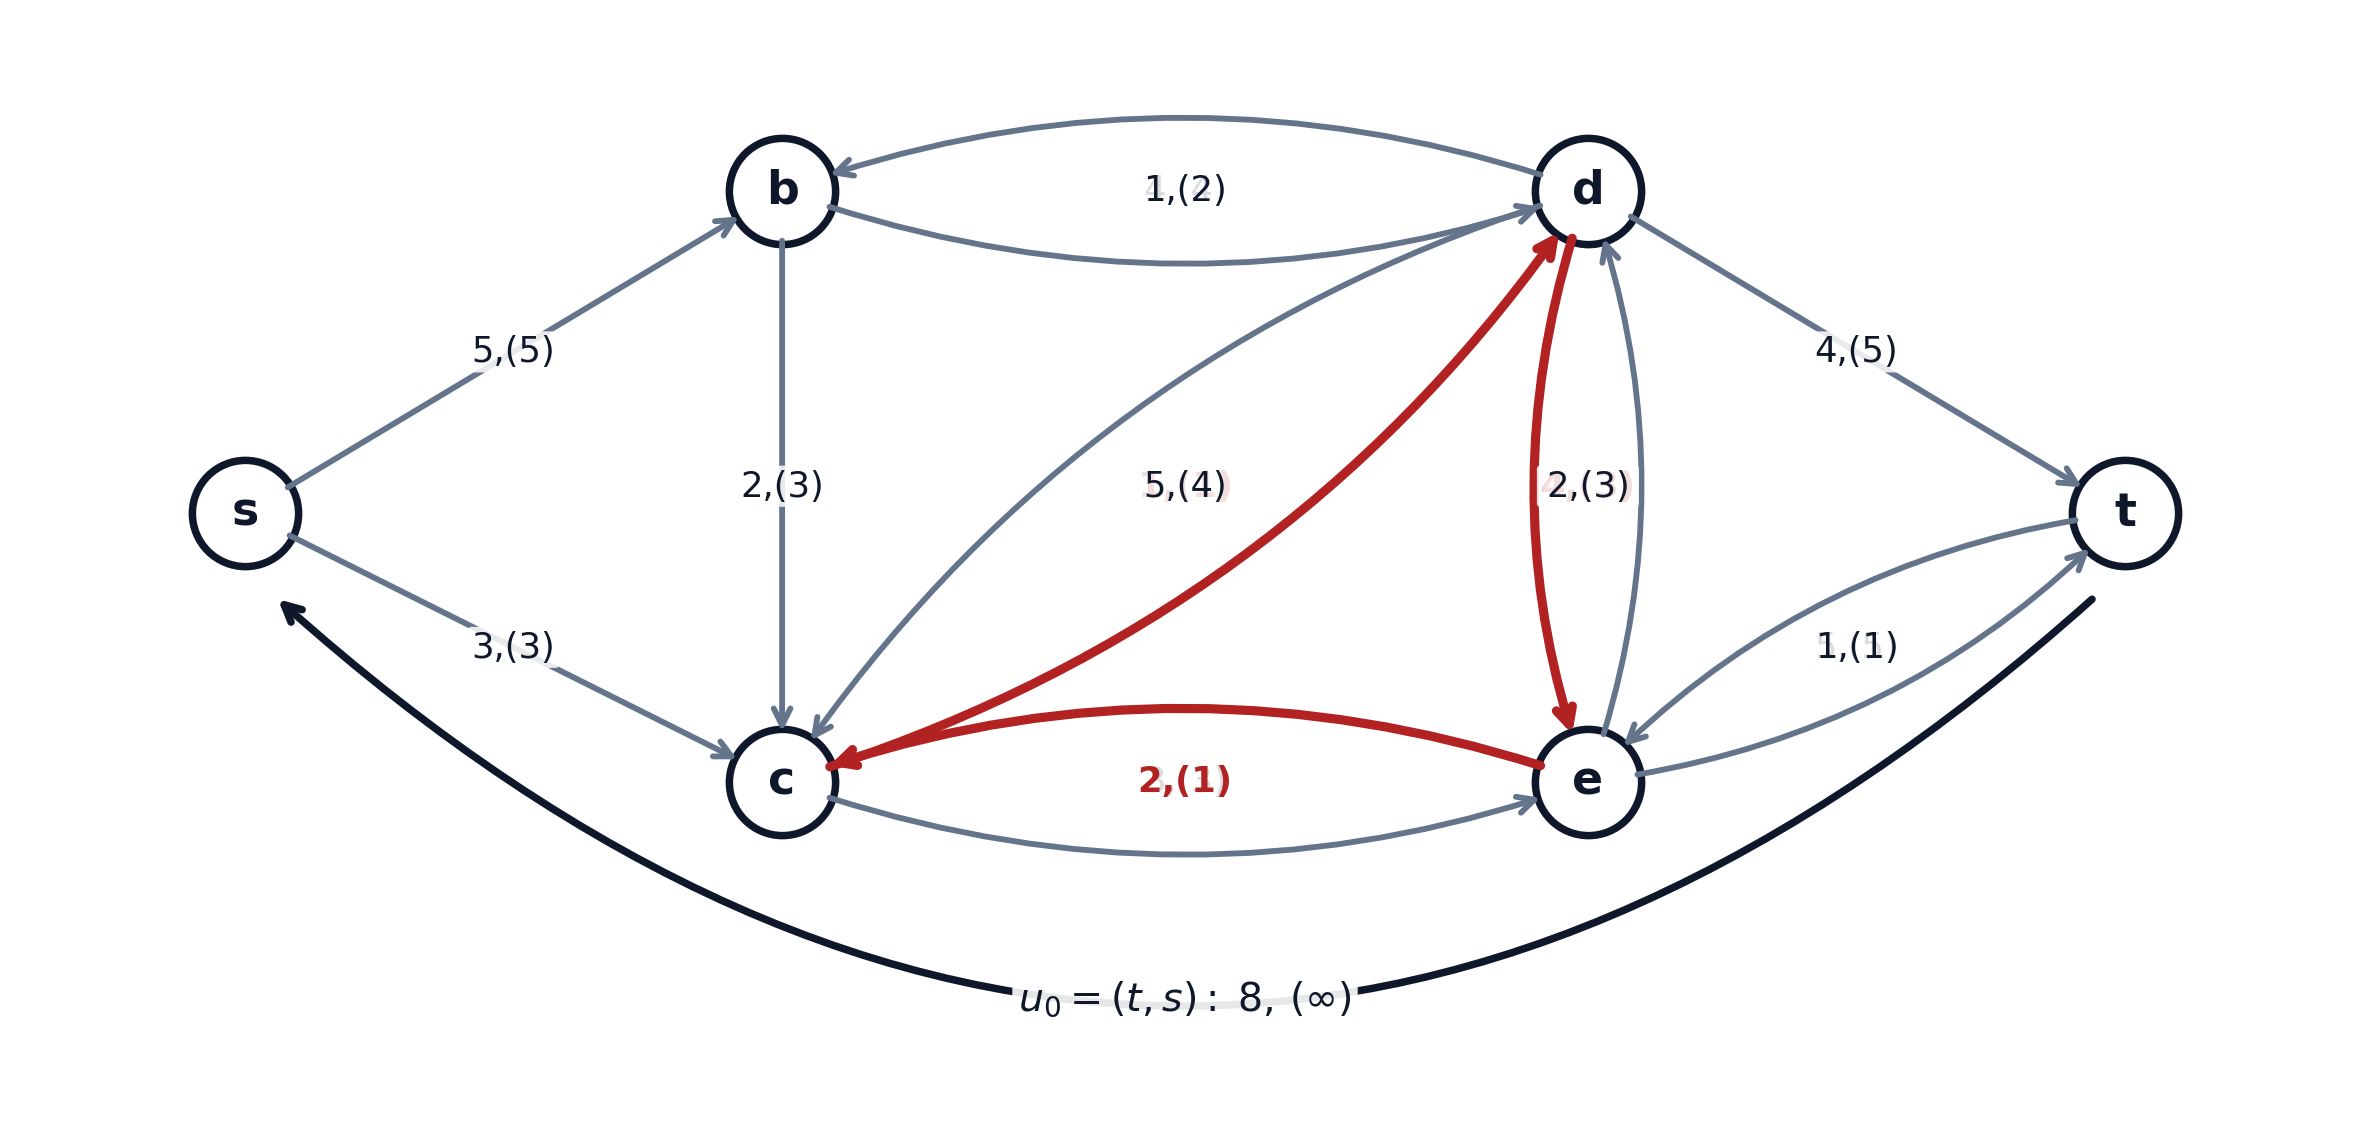
\includegraphics[width=0.85\linewidth,height=\textheight,keepaspectratio]{images/red_flujo_saturacion_ejemplo.png}

}

\caption{\label{fig-red-flujo-saturacion-ejemplo}Evaluación de
compatibilidad y detección de sobrecapacidad sobre la red de 6 nodos}

\end{figure}%

\end{tcolorbox}

Para comprender la gran versatilidad didáctica de las redes de
transporte, analicemos dos problemas prácticos de modelización: uno
proveniente de la ingeniería de tráfico urbano y otro de la optimización
combinatoria de tareas.

\begin{tcolorbox}[enhanced jigsaw, toprule=.15mm, opacitybacktitle=0.6, coltitle=black, colbacktitle=quarto-callout-tip-color!10!white, title=\textcolor{quarto-callout-tip-color}{\faLightbulb}\hspace{0.5em}{Ejemplo: Modelización de la capacidad de tráfico urbano}, arc=.35mm, rightrule=.15mm, toptitle=1mm, breakable, bottomtitle=1mm, titlerule=0mm, colback=white, opacityback=0, leftrule=.75mm, colframe=quarto-callout-tip-color-frame, left=2mm, bottomrule=.15mm]

La capacidad de tráfico de las calles de una ciudad se mide
habitualmente por el número máximo de automóviles que pueden circular
por ellas por minuto. En la red vial ilustrada en la
Figura~\ref{fig-red-trafico-ejemplo}, las intersecciones se representan
mediante vértices \(V = \{s, a, b, t\}\) y las calles dirigidas mediante
arcos con capacidades entre paréntesis \(c_u\):

\begin{itemize}
\tightlist
\item
  \(c_{sa} = 100\), \(c_{sb} = 100\), \(c_{ab} = 50\), \(c_{at} = 75\),
  \(c_{bt} = 100\).
\end{itemize}

Se desea determinar la cantidad máxima de automóviles por minuto que
pueden transitar desde la zona de entrada \(s\) hasta la zona de salida
\(t\).

\begin{figure}[H]

\centering{

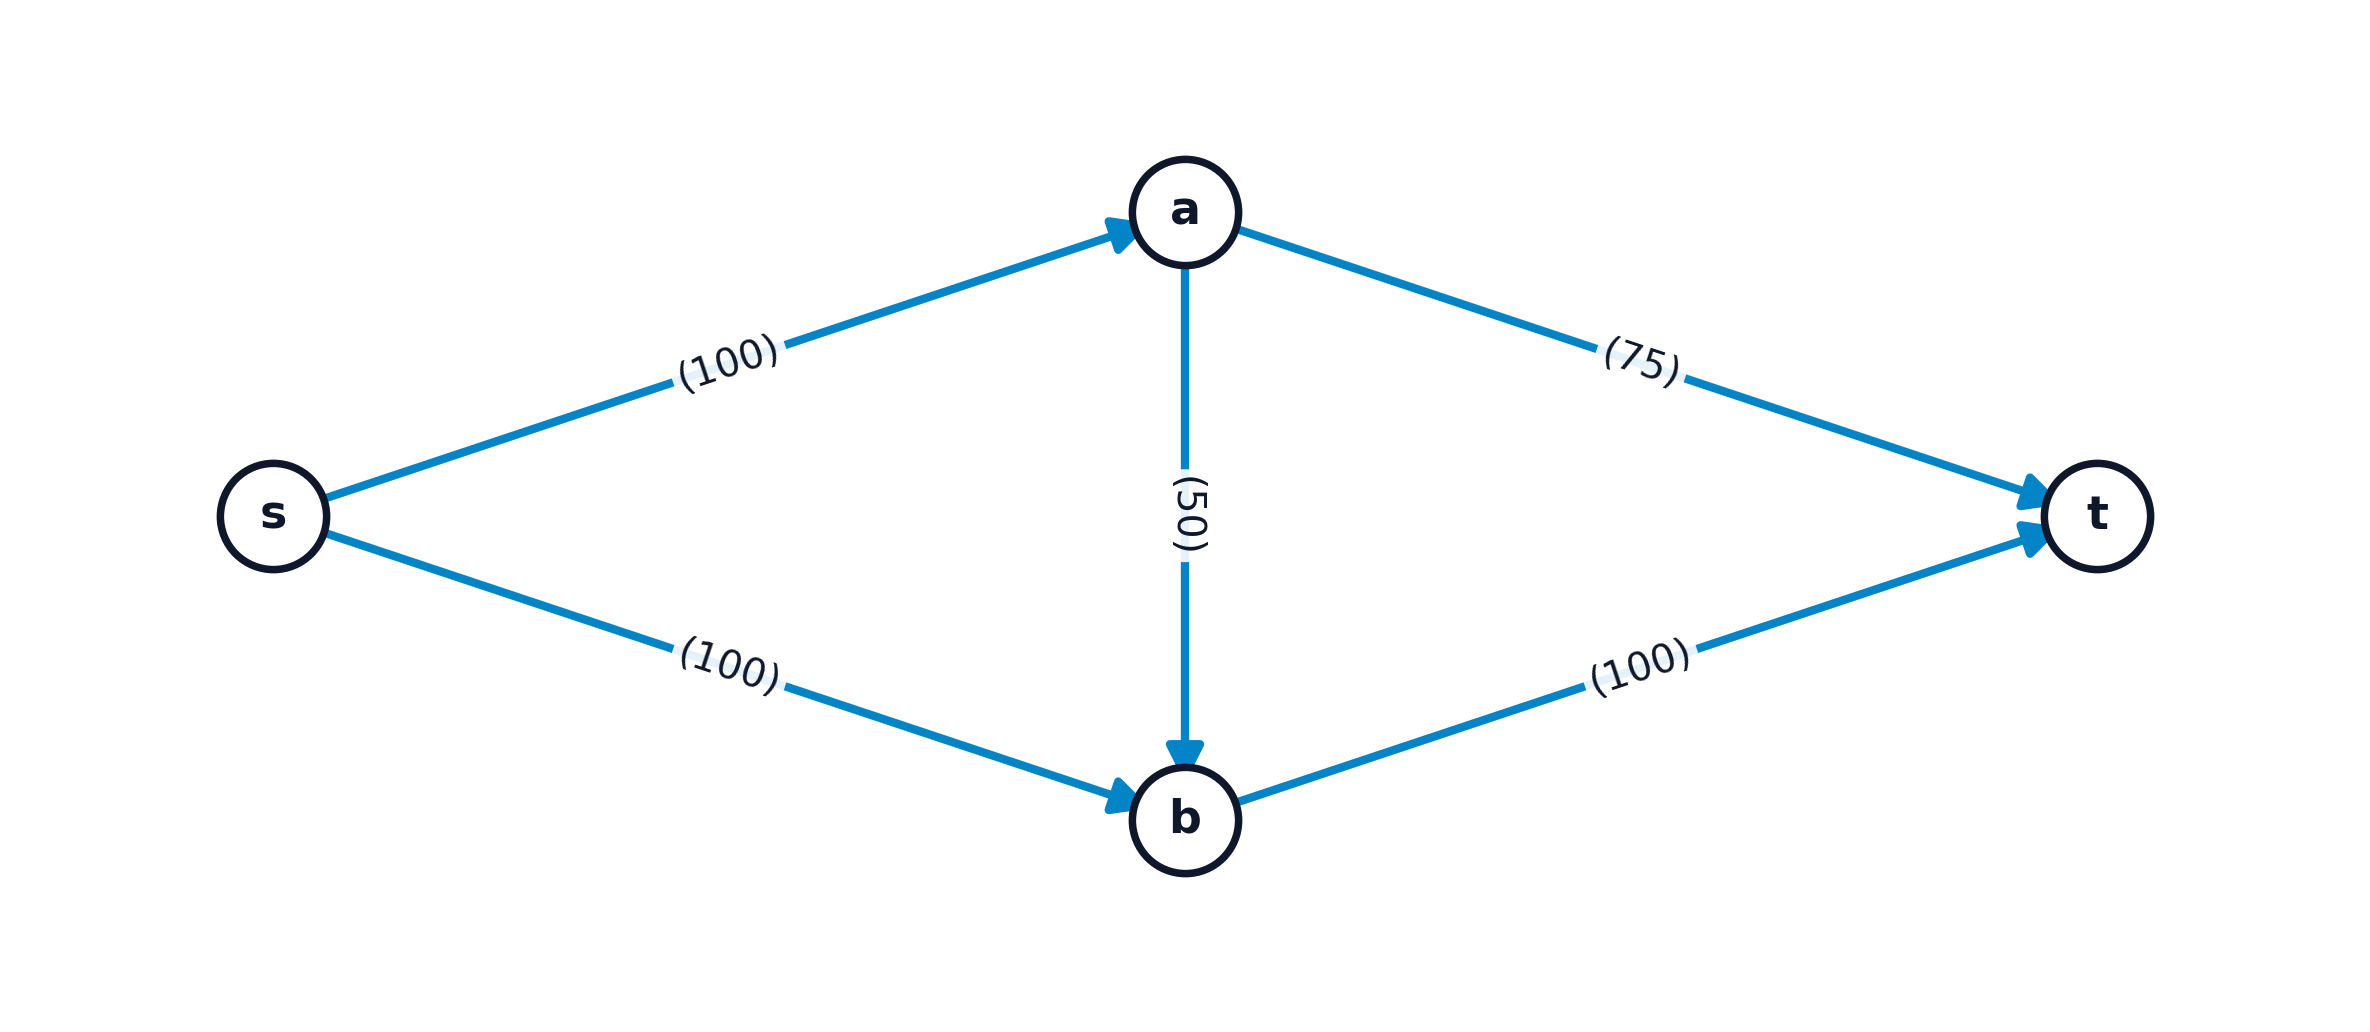
\includegraphics[width=0.65\linewidth,height=\textheight,keepaspectratio]{images/red_trafico_ejemplo.png}

}

\caption{\label{fig-red-trafico-ejemplo}Red de tráfico urbano con
capacidades de vehículos por minuto en los arcos}

\end{figure}%

Analizando la red, aunque la fuente \(s\) puede inyectar hasta
\(100 + 100 = 200\) vehículos/minuto hacia \(a\) y \(b\), las calles que
llegan al sumidero \(t\) restringen el cuello de botella: desde \(a\)
solo pueden llegar a \(t\) como máximo \(75\) vehículos/min, y desde
\(b\) hasta \(100\) vehículos/min. El valor del flujo máximo resulta ser
\(v(\mathbf{f}^*) = 175\) vehículos/min.

\end{tcolorbox}

Además de sistemas de transporte físico, el problema del flujo máximo
permite resolver de forma elegante problemas de optimización
combinatoria y asignación de personal.

\begin{tcolorbox}[enhanced jigsaw, toprule=.15mm, opacitybacktitle=0.6, coltitle=black, colbacktitle=quarto-callout-tip-color!10!white, title=\textcolor{quarto-callout-tip-color}{\faLightbulb}\hspace{0.5em}{Ejemplo: Asignación óptima de tareas a empleados (Emparejamiento
Bipartito)}, arc=.35mm, rightrule=.15mm, toptitle=1mm, breakable, bottomtitle=1mm, titlerule=0mm, colback=white, opacityback=0, leftrule=.75mm, colframe=quarto-callout-tip-color-frame, left=2mm, bottomrule=.15mm]

En una oficina hay tres empleados (\(E_1, E_2, E_3\)) y tres tareas
(\(T_1, T_2, T_3\)). Cada tarea requiere unos conocimientos específicos
que no todos los empleados poseen. Las compatibilidades se representan
en el digrafo bipartito de la Figura~\ref{fig-asignacion-tareas-ejemplo}
(izquierda):

\begin{itemize}
\tightlist
\item
  \(E_1\) es compatible con \(T_1, T_2\).
\item
  \(E_2\) es compatible con \(T_1, T_3\).
\item
  \(E_3\) es compatible con \(T_1, T_3\).
\end{itemize}

Se desea determinar cómo asignar las tareas a los empleados para tratar
de realizarlas todas (asignación uno a uno).

\begin{figure}[H]

\centering{

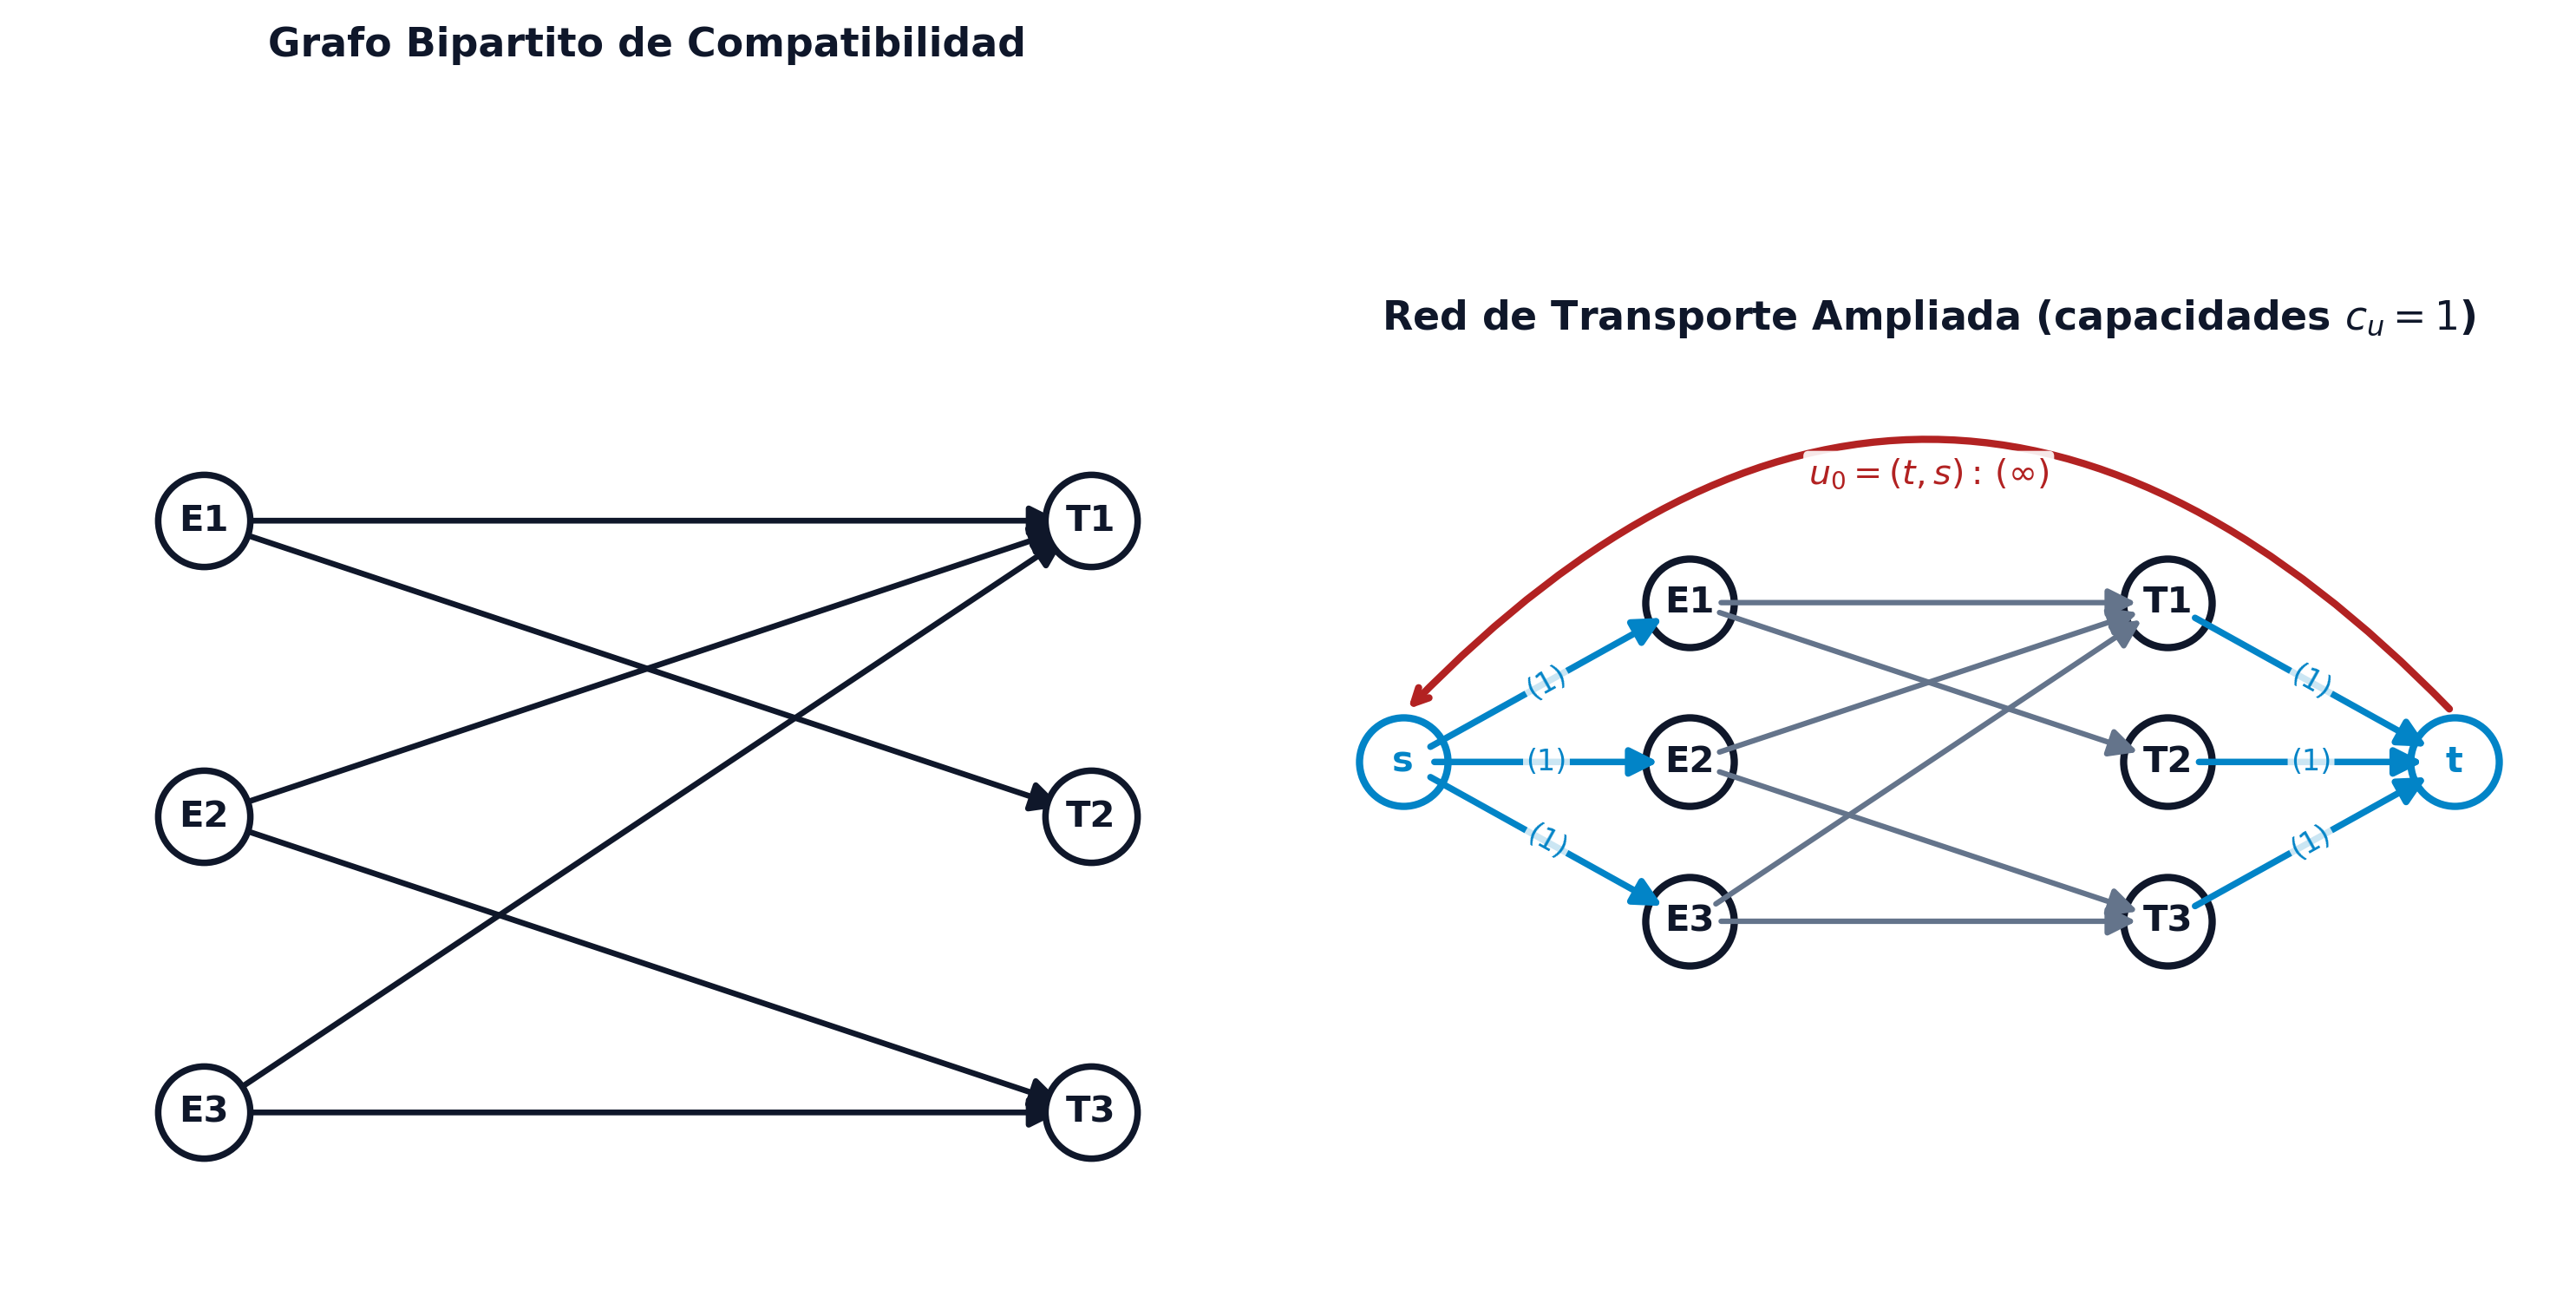
\includegraphics[width=0.95\linewidth,height=\textheight,keepaspectratio]{images/asignacion_tareas_ejemplo.png}

}

\caption{\label{fig-asignacion-tareas-ejemplo}Transformación de un
problema de asignación bipartita de tareas (izquierda) a una red de
transporte de flujo máximo con arco ficticio de retorno \(u_0=(t,s)\)
(derecha)}

\end{figure}%

\textbf{Modelización como problema de flujo máximo}: Para reducir este
problema a una red de transporte (derecha):

\begin{enumerate}
\def\labelenumi{\arabic{enumi}.}
\tightlist
\item
  Añadimos un nodo fuente ficticio \(s\) conectado a cada empleado
  \(E_i\) mediante un arco \((s, E_i)\) con capacidad \(c_{s E_i} = 1\)
  (cada empleado puede realizar como máximo 1 tarea).
\item
  Asignamos capacidad unitaria \(c_{E_i T_j} = 1\) a todos los arcos de
  compatibilidad entre empleados y tareas.
\item
  Añadimos un nodo sumidero ficticio \(t\) conectado desde cada tarea
  \(T_j\) mediante un arco \((T_j, t)\) con capacidad \(c_{T_j t} = 1\)
  (cada tarea requiere exactamente 1 empleado).
\item
  Añadimos el arco ficticio de retorno \(u_0 = (t, s)\) con capacidad
  ilimitada (\(c_0 = \infty\)).
\end{enumerate}

Resolver el flujo máximo de \(s\) a \(t\) sobre esta red equivale a
hallar el número máximo de tareas realizables simultáneamente.

\end{tcolorbox}

Una vez formalizada la red de transporte e ilustrada su versatilidad, el
esquema general para resolver cualquier problema de flujo máximo se
fundamenta en un procedimiento iterativo de aumento progresivo:

\begin{enumerate}
\def\labelenumi{\arabic{enumi}.}
\tightlist
\item
  \textbf{Flujo Inicial}: Comenzar con un flujo compatible válido
  \(\mathbf{f}^0\) sobre la red (típicamente el flujo trivial nulo
  \(\mathbf{f}^0 = \mathbf{0}\)).
\item
  \textbf{Búsqueda de Aumento}: Buscar un nuevo flujo compatible
  \(\mathbf{f}^{k+1}\) que incremente el valor circulante por el arco de
  retorno \(f_0\).
\item
  \textbf{Iteración y Criterio de Parada}: Repetir el procedimiento a
  partir del nuevo flujo hasta que no sea posible realizar ningún
  incremento adicional.
\end{enumerate}

La justificación matemática de este esquema radica en la estructura
algebraica del espacio de flujos: dado que todo flujo se puede expresar
como combinación lineal de ciclos, la diferencia entre dos soluciones
cualesquiera \(\mathbf{f}^2 - \mathbf{f}^1\) es siempre una
\textbf{combinación lineal de ciclos}. Por tanto, para elevar el caudal
de la fuente \(s\) al sumidero \(t\), el algoritmo analiza si existe en
la red un ciclo que incluya al arco ficticio de retorno \(u_0 = (t, s)\)
y admita un incremento de al menos una unidad de flujo. Esta búsqueda
equivale a encontrar una trayectoria no saturada en sentido directo
desde \(s\) hasta \(t\), denominada \textbf{cadena incremental}.

\begin{tcolorbox}[enhanced jigsaw, toprule=.15mm, opacitybacktitle=0.6, coltitle=black, colbacktitle=quarto-callout-note-color!10!white, title=\textcolor{quarto-callout-note-color}{\faInfo}\hspace{0.5em}{Definición: Cadena incremental y ciclo incremental}, arc=.35mm, rightrule=.15mm, toptitle=1mm, breakable, bottomtitle=1mm, titlerule=0mm, colback=white, opacityback=0, leftrule=.75mm, colframe=quarto-callout-note-color-frame, left=2mm, bottomrule=.15mm]

Dado un flujo compatible \(\mathbf{f}\) en la red de transporte
\((G = (V, U), \mathbf{c})\), una cadena \(\mu[a, b]\) entre dos
vértices \(a\) y \(b\) es una \textbf{cadena incremental} (o camino
aumentante) si satisface:

\[
f_u < c_u, \quad \forall u \in \mu^+ \qquad \text{y} \qquad f_u > 0, \quad \forall u \in \mu^-
\]

donde \(\mu^+\) representa el conjunto de arcos de la cadena recorridos
en sentido directo (de \(a\) hacia \(b\)) y \(\mu^-\) representa los
arcos recorridos en sentido inverso.

Un \textbf{ciclo incremental} es una cadena incremental cerrada. En el
problema del flujo máximo, el objetivo es incrementar el flujo
transportado por el arco de retorno \(u_0 = (t, s)\), por lo que se
busca sistemáticamente una cadena incremental entre la fuente \(s\) y el
sumidero \(t\).

\end{tcolorbox}

\begin{tcolorbox}[enhanced jigsaw, toprule=.15mm, opacitybacktitle=0.6, coltitle=black, colbacktitle=quarto-callout-note-color!10!white, title=\textcolor{quarto-callout-note-color}{\faInfo}\hspace{0.5em}{Definición: Capacidad residual de una cadena}, arc=.35mm, rightrule=.15mm, toptitle=1mm, breakable, bottomtitle=1mm, titlerule=0mm, colback=white, opacityback=0, leftrule=.75mm, colframe=quarto-callout-note-color-frame, left=2mm, bottomrule=.15mm]

La \textbf{capacidad residual} \(c(\mu)\) (o cuello de botella) de una
cadena incremental \(\mu[s, t]\) es la máxima cantidad de flujo
adicional que se puede enviar desde \(s\) hasta \(t\) a través de
\(\mu\):

\[
c(\mu) = \min \left\{ \min_{u \in \mu^+} (c_u - f_u), \, \min_{u \in \mu^-} f_u \right\}
\]

\end{tcolorbox}

Si se incrementa el flujo en \(c(\mu)\) unidades en los arcos directos
\(u \in \mu^+\) y se reduce en \(c(\mu)\) unidades en los arcos inversos
\(u \in \mu^-\), el valor total del flujo \(f_0\) aumenta exactamente en
\(c(\mu)\) unidades manteniendo la compatibilidad estricta.

\subsection{Flujo máximo en grafos no
dirigidos}\label{flujo-muxe1ximo-en-grafos-no-dirigidos}

En el caso de redes construidas sobre un grafo no dirigido
\(G = (V, E)\), el problema de flujo no queda bien definido de forma
directa sobre las aristas. La capacidad \(c_e\) de una arista no
dirigida \(e = \{a, b\} \in E\) puede ser saturada en el sentido de
tránsito \((a, b)\) o en el sentido contrario \((b, a)\).

Para evitar enviar flujo en los dos sentidos simultáneamente de modo que
se verifique \(f_{(a,b)} + f_{(b,a)} \le c_e\) siendo ambos flujos
positivos, es necesario transformar el grafo original en un digrafo
equivalente de forma que se impida el flujo en sentido inverso sobre una
misma arista.

\begin{tcolorbox}[enhanced jigsaw, toprule=.15mm, opacitybacktitle=0.6, coltitle=black, colbacktitle=quarto-callout-note-color!10!white, title=\textcolor{quarto-callout-note-color}{\faInfo}\hspace{0.5em}{Definición: Transformación de aristas no dirigidas (Gadget de 5 arcos)}, arc=.35mm, rightrule=.15mm, toptitle=1mm, breakable, bottomtitle=1mm, titlerule=0mm, colback=white, opacityback=0, leftrule=.75mm, colframe=quarto-callout-note-color-frame, left=2mm, bottomrule=.15mm]

Cada arista no dirigida \(e = \{a, b\} \in E\) con capacidad \(c_e = c\)
se sustituye por un conjunto de \textbf{cinco arcos dirigidos} que
conectan los vértices originales \(a\) y \(b\) con dos nuevos vértices
auxiliares \(a'\) y \(b'\), asignando capacidad \(c\) a todos ellos:

\[
U_e = \{ (a, a'), \, (b, a'), \, (a', b'), \, (b', a), \, (b', b) \}
\]

\end{tcolorbox}

\begin{figure}

\centering{

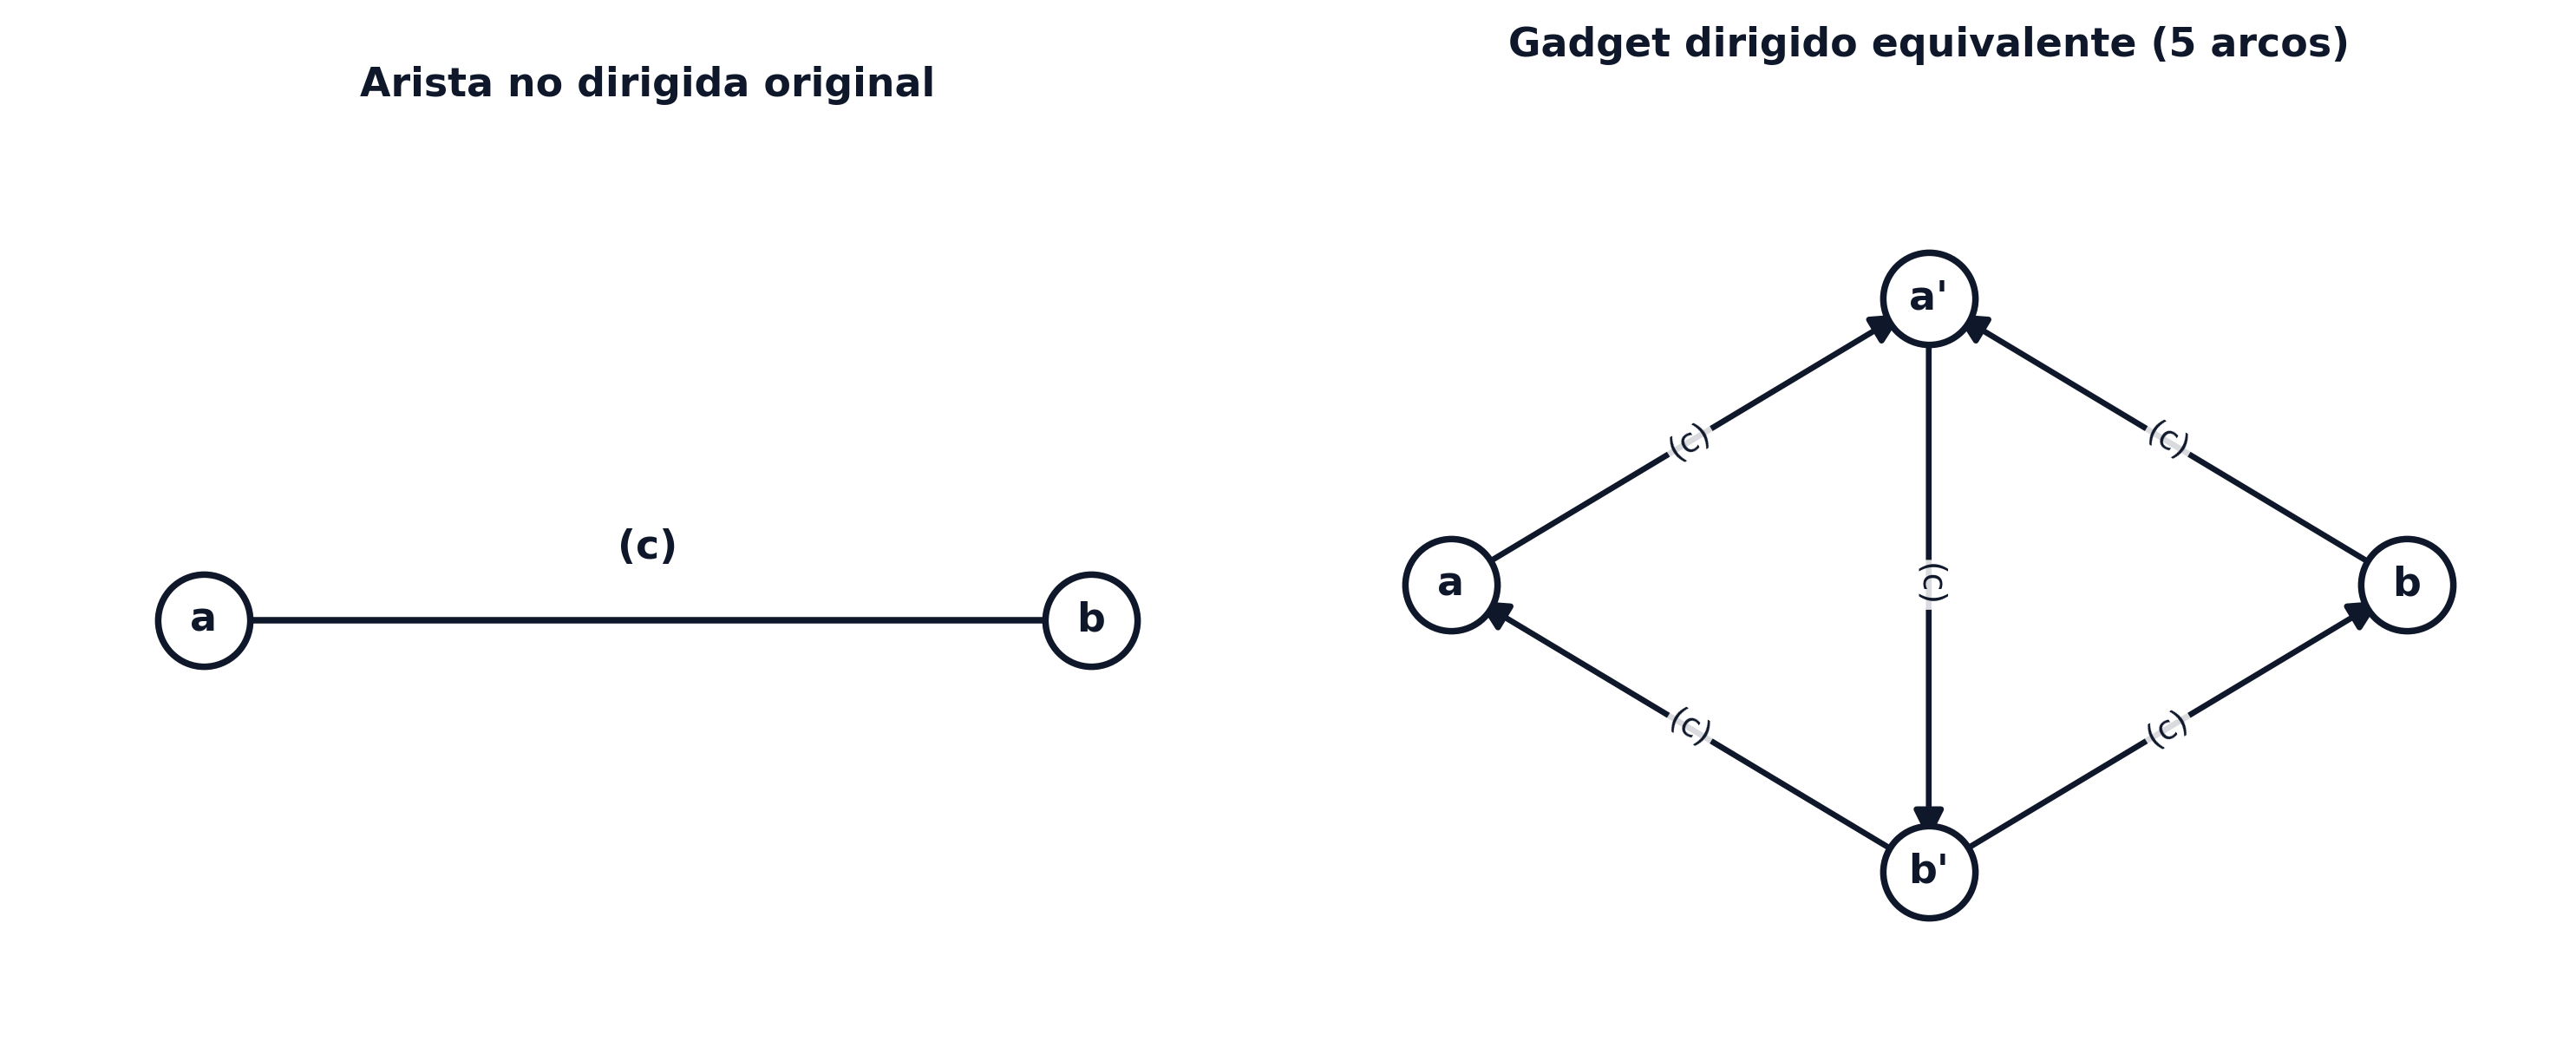
\includegraphics[width=0.75\linewidth,height=\textheight,keepaspectratio]{images/transformacion_arista_nodirigida.png}

}

\caption{\label{fig-transformacion-arista-nodirigida}Transformación de
una arista no dirigida \(\{a, b\}\) de capacidad \(c\) (izquierda) en un
gadget dirigido equivalente de 5 arcos y 2 nodos auxiliares \(a', b'\)
(derecha)}

\end{figure}%

Como se ilustra en la Figura~\ref{fig-transformacion-arista-nodirigida},
esta construcción garantiza la equivalencia física y matemática:

\begin{itemize}
\tightlist
\item
  \textbf{Tránsito de \(a\) hacia \(b\)}: El flujo sigue el camino
  \(a \to a' \to b' \to b\), quedando limitado por la capacidad \(c\)
  del arco central \((a', b')\).
\item
  \textbf{Tránsito de \(b\) hacia \(a\)}: El flujo sigue el camino
  \(b \to a' \to b' \to a\), atravesando exactamente el mismo arco
  central \((a', b')\).
\end{itemize}

Dado que ambas direcciones deben atravesar de forma obligatoria el arco
central dirigido \((a', b')\), se satisface de forma automática la
restricción global \(f_{(a,b)} + f_{(b,a)} \le c\), impidiendo la
circulación simultánea en ambos sentidos y manteniendo la compatibilidad
estricta.

\subsection{Flujo máximo y corte
mínimo}\label{flujo-muxe1ximo-y-corte-muxednimo}

La búsqueda de la cantidad máxima de caudal que puede transitar desde la
fuente \(s\) hasta el sumidero \(t\) conduce de forma natural al estudio
de los cuellos de botella topológicos que restringen la red. La
capacidad global de transmisión no está determinada únicamente por las
conexiones individuales, sino por barreras o particiones completas que
separan físicamente el origen del destino.

\begin{tcolorbox}[enhanced jigsaw, toprule=.15mm, opacitybacktitle=0.6, coltitle=black, colbacktitle=quarto-callout-note-color!10!white, title=\textcolor{quarto-callout-note-color}{\faInfo}\hspace{0.5em}{Definición: \((s, t)\)-Corte}, arc=.35mm, rightrule=.15mm, toptitle=1mm, breakable, bottomtitle=1mm, titlerule=0mm, colback=white, opacityback=0, leftrule=.75mm, colframe=quarto-callout-note-color-frame, left=2mm, bottomrule=.15mm]

Dada la red de transporte \((G = (V, U), \mathbf{c})\), un \textbf{corte
que separa \(s\) y \(t\)} o \textbf{\((s, t)\)-corte} es un conjunto de
arcos salientes \(w^+(N)\) asociado a un subconjunto de vértices
\(N \subset V\) tal que \(s \in N\) y \(t \notin N\).

\end{tcolorbox}

Para evaluar cuantitativamente el cuello de botella que representa una
partición \(N\), es preciso sumar la capacidad máxima de todas las
conducciones que abandonan el conjunto \(N\) hacia su complemento
\(V \setminus N\).

\begin{tcolorbox}[enhanced jigsaw, toprule=.15mm, opacitybacktitle=0.6, coltitle=black, colbacktitle=quarto-callout-note-color!10!white, title=\textcolor{quarto-callout-note-color}{\faInfo}\hspace{0.5em}{Definición: Capacidad de un corte}, arc=.35mm, rightrule=.15mm, toptitle=1mm, breakable, bottomtitle=1mm, titlerule=0mm, colback=white, opacityback=0, leftrule=.75mm, colframe=quarto-callout-note-color-frame, left=2mm, bottomrule=.15mm]

Dada la red de transporte \((G = (V, U), \mathbf{c})\), se define la
\textbf{capacidad de un \((s, t)\)-corte} como la suma de las
capacidades de los arcos que lo componen:

\[
c(w^+(N)) = \sum_{u \in w^+(N)} c_u
\]

\end{tcolorbox}

De todas las posibles particiones que separan la fuente del sumidero,
aquellas que imponen la restricción más severa constituyen los cuellos
de botella verdaderamente críticos de la infraestructura.

\begin{tcolorbox}[enhanced jigsaw, toprule=.15mm, opacitybacktitle=0.6, coltitle=black, colbacktitle=quarto-callout-note-color!10!white, title=\textcolor{quarto-callout-note-color}{\faInfo}\hspace{0.5em}{Definición: Problema de corte de mínima capacidad}, arc=.35mm, rightrule=.15mm, toptitle=1mm, breakable, bottomtitle=1mm, titlerule=0mm, colback=white, opacityback=0, leftrule=.75mm, colframe=quarto-callout-note-color-frame, left=2mm, bottomrule=.15mm]

El \textbf{problema de corte de mínima capacidad} trata de determinar en
una red de transporte el \((s, t)\)-corte cuya capacidad sea mínima:

\[
\min_{\substack{N \subset V \\ s \in N, \, t \notin N}} c(w^+(N)) = \sum_{u \in w^+(N)} c_u
\]

\end{tcolorbox}

Existe una relación dual fundamental entre el flujo \(f_0\) que circula
por la red y la capacidad de cualquier \((s, t)\)-corte. El siguiente
resultado establece que ningún flujo puede superar la capacidad de la
barrera más estrecha que deba atravesar.

\begin{tcolorbox}[enhanced jigsaw, toprule=.15mm, opacitybacktitle=0.6, coltitle=black, colbacktitle=quarto-callout-note-color!10!white, title=\textcolor{quarto-callout-note-color}{\faInfo}\hspace{0.5em}{Proposición: Acotación del flujo por la capacidad del corte}, arc=.35mm, rightrule=.15mm, toptitle=1mm, breakable, bottomtitle=1mm, titlerule=0mm, colback=white, opacityback=0, leftrule=.75mm, colframe=quarto-callout-note-color-frame, left=2mm, bottomrule=.15mm]

Dada una red de transporte \((G = (V, U), \mathbf{c})\) y fijados los
vértices \(s, t \in V\), para cualquier \((s, t)\)-flujo compatible
\(\mathbf{f}\) se verifica que su valor de flujo \(f_0\) está acotado
por la capacidad de cualquier \((s, t)\)-corte. Es decir:

\[
f_0 \le \sum_{u \in w^+(N)} c_u, \qquad \forall N \subset V \text{ tal que } s \in N, \, t \notin N
\]

\emph{Demostración}: Sea \(N \subset V\) tal que \(s \in N\) y
\(t \notin N\). Sea \(\mathbf{f} = (f_0, f_1, \dots, f_m)\) un flujo
compatible en la red ampliada con el arco ficticio de retorno
\(u_0 = (t, s)\).

Por la ley de conservación de flujo en los nodos del conjunto \(N\), la
suma de los flujos que entran en \(N\) es igual a la suma de los flujos
que salen de \(N\):

\[
f_0 + \sum_{\substack{(i,j) \in w^-(N) \\ (i,j) \neq (t,s)}} f_{ij} = \sum_{(i,j) \in w^+(N)} f_{ij}
\]

Reordenando términos para aislar el valor del flujo circulante \(f_0\):

\[
f_0 = \sum_{(i,j) \in w^+(N)} f_{ij} - \sum_{\substack{(i,j) \in w^-(N) \\ (i,j) \neq (t,s)}} f_{ij}
\]

Como \(0 \le f_{ij} \le c_{ij}, \, \forall (i, j) \in U\), acotamos los
dos sumandos: la suma de flujos entrantes es no negativa
(\(\sum f_{ij} \ge 0\)) y la suma de flujos salientes no puede superar
sus capacidades limitadas (\(\sum f_{ij} \le \sum c_{ij}\)). Por
consiguiente:

\[
f_0 \le \sum_{(i,j) \in w^+(N)} c_{ij} = c(w^+(N))
\]

Esta cota es válida para cualquier partición \(N \subset V\) con
\(s \in N, t \notin N\) y para cada flujo \(\mathbf{f}\) compatible con
las capacidades. En particular, se verifica también para el flujo que
maximiza \(f_0\), estableciendo que el flujo máximo está acotado por el
corte de capacidad mínima:

\[
\max f_0 \le \min_{\substack{N \subset V \\ s \in N, \, t \notin N}} \left\{ \sum_{(i,j) \in w^+(N)} c_{ij} \right\} \quad \blacksquare
\]

\end{tcolorbox}

\begin{tcolorbox}[enhanced jigsaw, toprule=.15mm, opacitybacktitle=0.6, coltitle=black, colbacktitle=quarto-callout-tip-color!10!white, title=\textcolor{quarto-callout-tip-color}{\faLightbulb}\hspace{0.5em}{Ejemplo: Evaluación de cortes, capacidades y criterio de optimalidad}, arc=.35mm, rightrule=.15mm, toptitle=1mm, breakable, bottomtitle=1mm, titlerule=0mm, colback=white, opacityback=0, leftrule=.75mm, colframe=quarto-callout-tip-color-frame, left=2mm, bottomrule=.15mm]

Considérese la red de transporte de 6 nodos \(V = \{s, b, c, d, e, t\}\)
ilustrada en la Figura~\ref{fig-red-cortes-ejemplo}, equipada con las
capacidades entre paréntesis \(c_u\) y transitando con un
\((s, t)\)-flujo compatible de valor \(f_0 = 8\).

Evaluamos tres cortes representativos \(w^+(N)\) que separan la fuente
\(s\) del sumidero \(t\):

\begin{enumerate}
\def\labelenumi{\arabic{enumi}.}
\tightlist
\item
  \textbf{Corte 1 (\(N_1 = \{s\}\))} (línea discontinua \textbf{roja
  teja}):

  \begin{itemize}
  \tightlist
  \item
    Arcos salientes: \(w^+(N_1) = \{(s, b), (s, c)\}\).
  \item
    Capacidad del corte: \(c(w^+(N_1)) = c_{sb} + c_{sc} = 5 + 3 = 8\).
  \end{itemize}
\item
  \textbf{Corte 2 (\(N_2 = \{s, b, c\}\))} (línea discontinua
  \textbf{azul cerúleo}):

  \begin{itemize}
  \tightlist
  \item
    Arcos salientes: \(w^+(N_2) = \{(b, d), (c, d), (c, e)\}\).
  \item
    Capacidad del corte:
    \(c(w^+(N_2)) = c_{bd} + c_{cd} + c_{ce} = 4 + 4 + 3 = 11\).
  \end{itemize}
\item
  \textbf{Corte 3 (\(N_3 = \{s, b, c, d, e\}\))} (línea discontinua
  \textbf{magenta}):

  \begin{itemize}
  \tightlist
  \item
    Arcos salientes: \(w^+(N_3) = \{(d, t), (e, t)\}\).
  \item
    Capacidad del corte: \(c(w^+(N_3)) = c_{dt} + c_{et} = 5 + 5 = 10\).
  \end{itemize}
\end{enumerate}

\begin{figure}[H]

\centering{

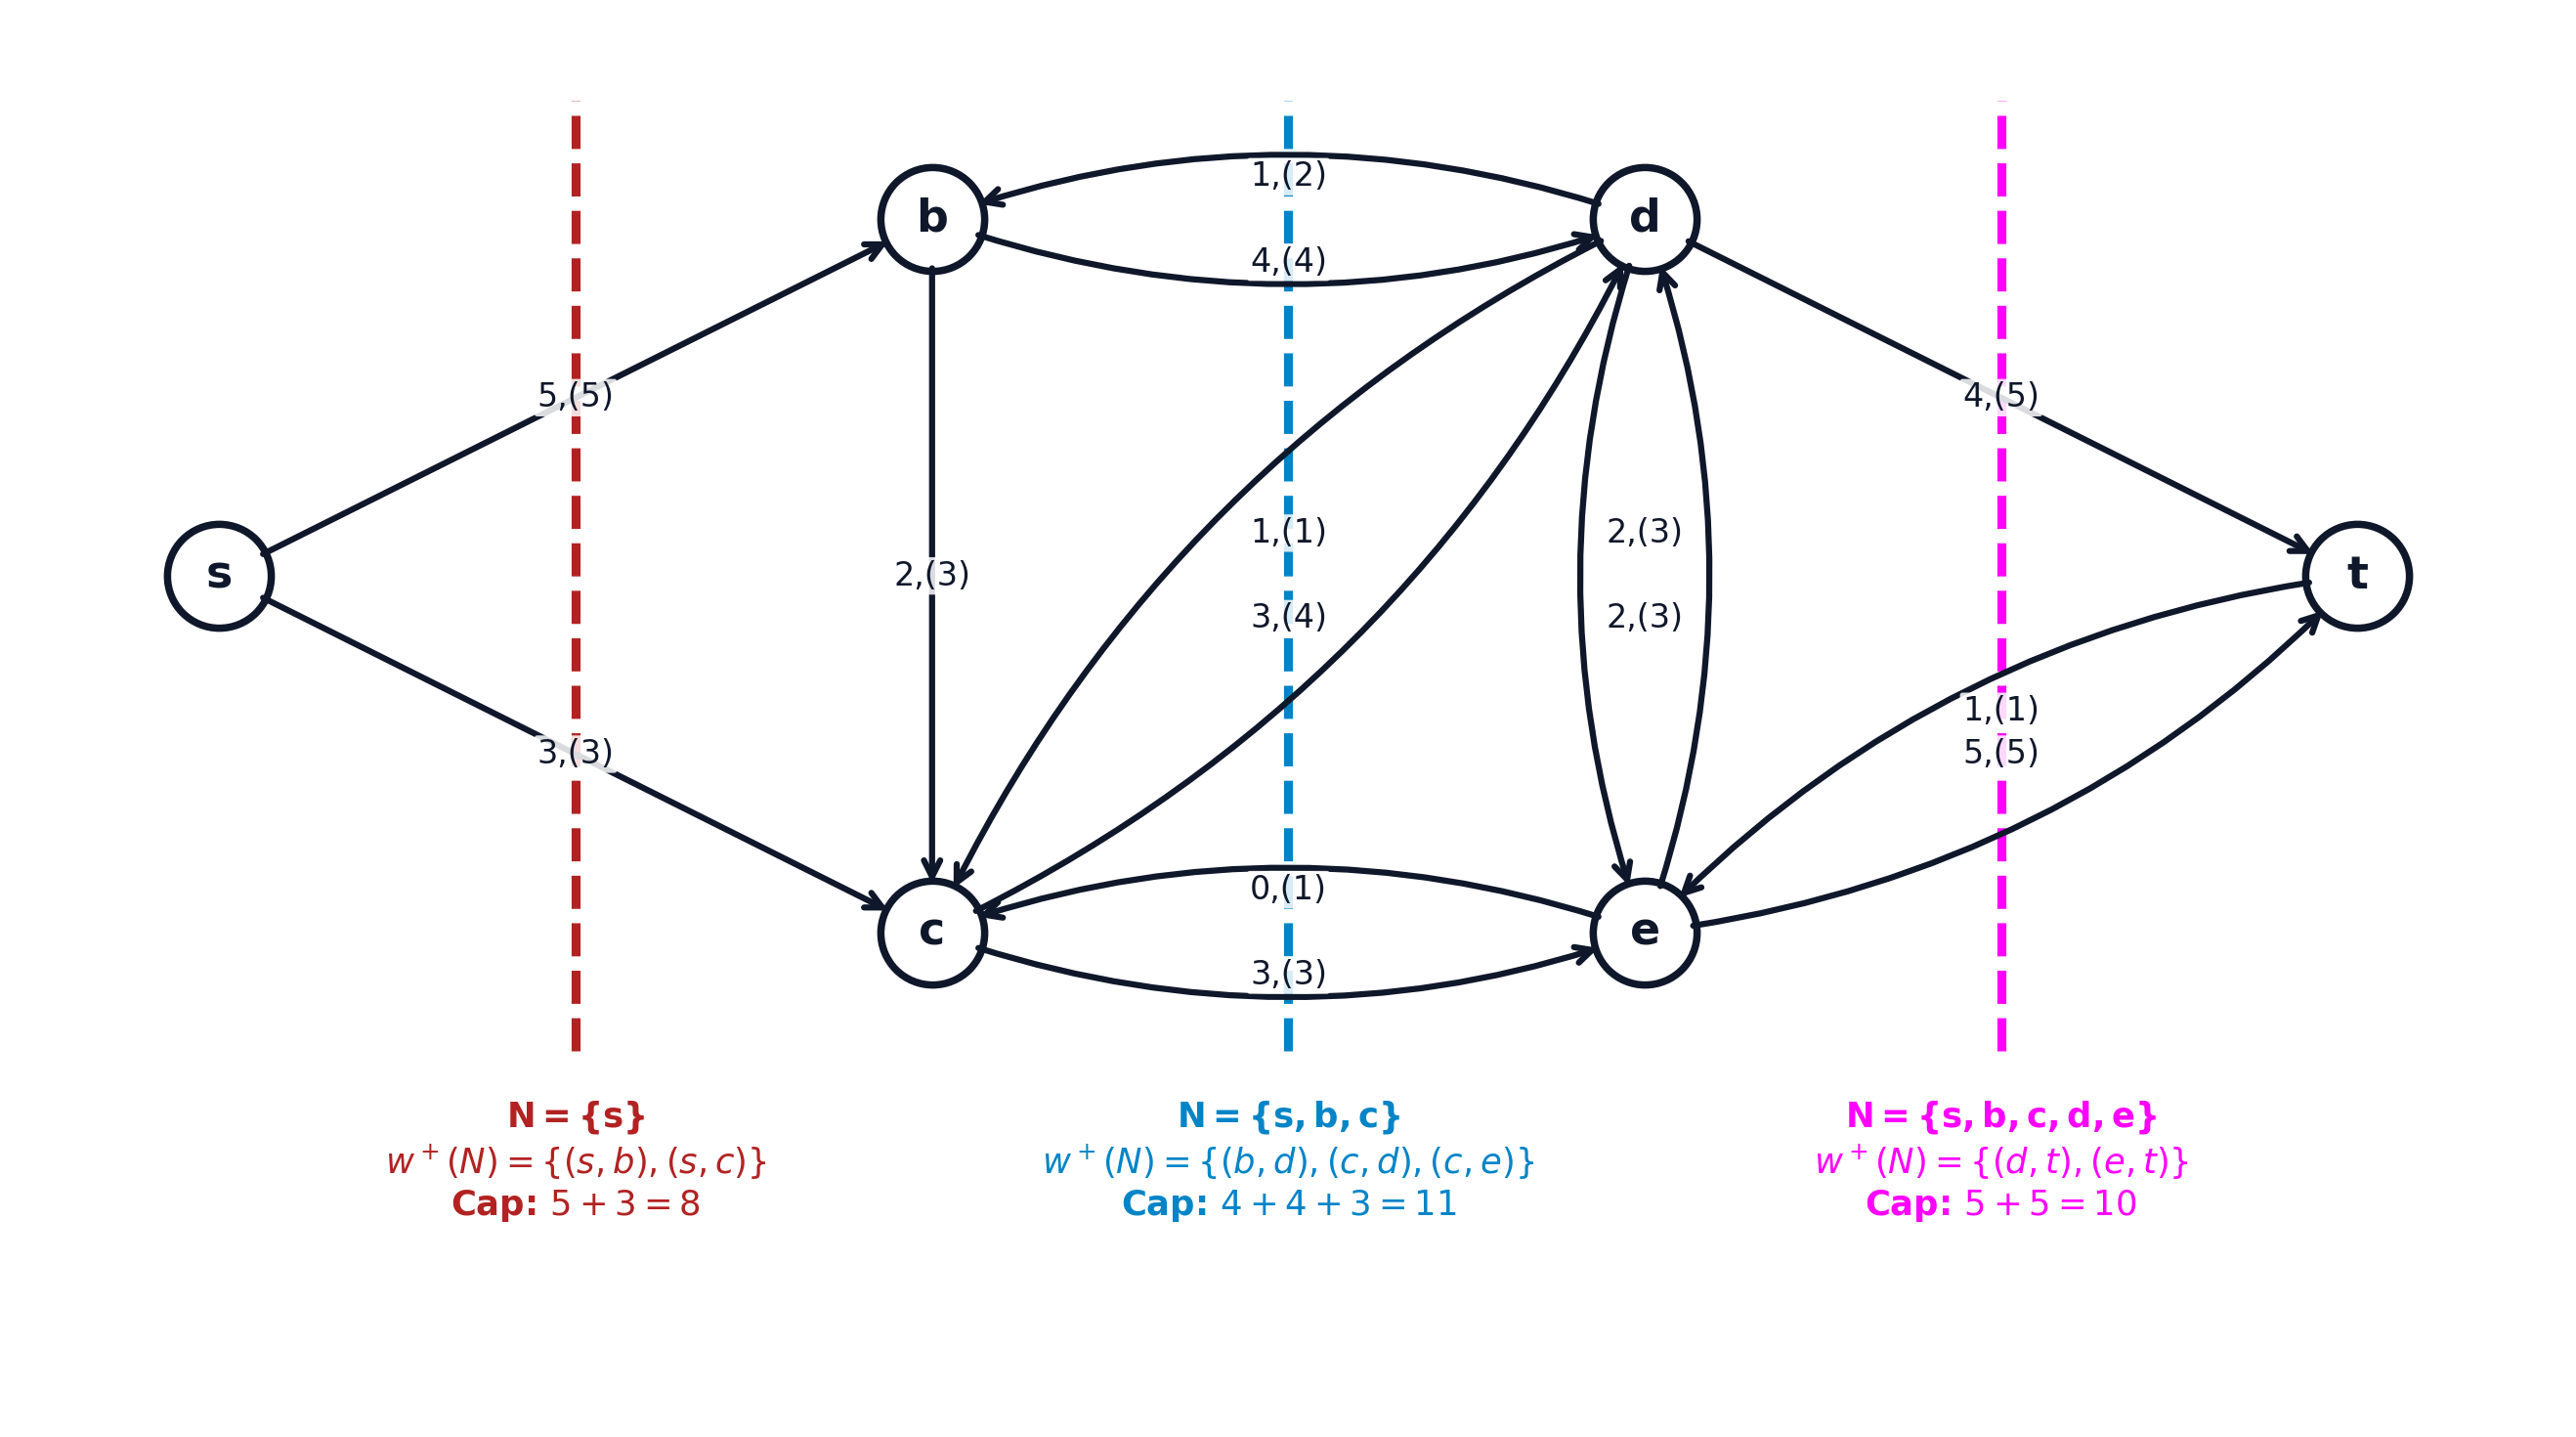
\includegraphics[width=0.85\linewidth,height=\textheight,keepaspectratio]{images/red_cortes_ejemplo.png}

}

\caption{\label{fig-red-cortes-ejemplo}Evaluación de cortes y
capacidades en una red de 6 nodos}

\end{figure}%

\textbf{Criterio de Optimalidad}: La capacidad del corte rojo
\(w^+(N_1)\) es \(c(w^+(N_1)) = 8\) y el valor del flujo que transita de
\(s\) a \(t\) es \(f_0 = 8\).

Dado que el valor del flujo alcanza exactamente la capacidad del corte
(\(f_0 = c(w^+(N_1)) = 8\)), por la Proposición de Acotación, este flujo
\(\mathbf{f}\) es una \textbf{solución óptima al problema del flujo
máximo} y el corte \(w^+(N_1)\) es un \textbf{corte de capacidad
mínima}.

\end{tcolorbox}

Como consecuencia inmediata de esta cota superior, si se encuentra una
pareja formada por un flujo compatible y un \((s, t)\)-corte cuyas
magnitudes numéricas coincidan, queda garantizada de forma simultánea la
optimalidad global de ambos elementos.

\begin{tcolorbox}[enhanced jigsaw, toprule=.15mm, opacitybacktitle=0.6, coltitle=black, colbacktitle=quarto-callout-note-color!10!white, title=\textcolor{quarto-callout-note-color}{\faInfo}\hspace{0.5em}{Corolario: Criterio de optimalidad de flujo máximo y corte mínimo}, arc=.35mm, rightrule=.15mm, toptitle=1mm, breakable, bottomtitle=1mm, titlerule=0mm, colback=white, opacityback=0, leftrule=.75mm, colframe=quarto-callout-note-color-frame, left=2mm, bottomrule=.15mm]

Si un flujo compatible \(\mathbf{f}\) y un \((s, t)\)-corte \(w^+(N)\)
que separe \(s\) de \(t\) son tales que el valor del flujo es igual a la
capacidad del corte (\(f_0 = c(w^+(N))\)), entonces \(\mathbf{f}\) es el
\textbf{flujo máximo} de \(s\) a \(t\) y \(w^+(N)\) es el \textbf{corte
de mínima capacidad} que separa \(s\) de \(t\).

\emph{Demostración}: La demostración es trivial. Dado que por la
proposición previa se verifica \(f'_0 \le c(w^+(N'))\) para cualquier
flujo compatible \(\mathbf{f}'\) y cualquier corte \(N'\), si
\(f_0 = c(w^+(N))\), ningún otro flujo compatible \(\mathbf{f}'\) puede
tener un valor superior a \(c(w^+(N)) = f_0\), de lo que se deduce que
\(\mathbf{f}\) es óptimo. De forma análoga, ningún otro corte \(N'\)
puede tener una capacidad inferior a \(f_0 = c(w^+(N))\), por lo que
\(w^+(N)\) es un corte de capacidad mínima. \(\blacksquare\)

\end{tcolorbox}

Además de caracterizar la optimalidad mediante la coincidencia entre el
flujo y el corte, resulta fundamental determinar las condiciones
estructurales bajo las cuales el problema del flujo máximo admite una
solución finita o, por el contrario, su valor óptimo diverge a infinito.

\begin{tcolorbox}[enhanced jigsaw, toprule=.15mm, opacitybacktitle=0.6, coltitle=black, colbacktitle=quarto-callout-note-color!10!white, title=\textcolor{quarto-callout-note-color}{\faInfo}\hspace{0.5em}{Corolario: Existencia y acotación de solución del problema de flujo
máximo}, arc=.35mm, rightrule=.15mm, toptitle=1mm, breakable, bottomtitle=1mm, titlerule=0mm, colback=white, opacityback=0, leftrule=.75mm, colframe=quarto-callout-note-color-frame, left=2mm, bottomrule=.15mm]

El problema del flujo máximo de \(s\) a \(t\) tiene solución finita si y
sólo si no existe un camino orientado de \(s\) a \(t\), denotado por
\(\mu[s, t]\), con capacidad infinita en todos sus arcos
(\(c_u = \infty, \, \forall u \in \mu\)).

\emph{Demostración}:

\begin{itemize}
\item
  Implicación directa (\(\implies\)): La demostración es trivial. Si
  existiera un camino \(\mu[s, t]\) formado íntegramente por arcos de
  capacidad infinita, se podría enviar una cantidad arbitrariamente
  grande de caudal a través de él sin violar ninguna restricción de
  capacidad, haciendo que el valor del flujo \(f_0 \to \infty\) y el
  problema no posea solución finita.
\item
  Implicación contraria (\(\impliedby\)): Supóngase que no existe ningún
  camino orientado desde \(s\) hasta \(t\) compuesto únicamente por
  arcos de capacidad infinita. Consideremos el grafo parcial
  \(G' = (V, U_{\infty})\) formado por todos los vértices \(V\) y el
  subconjunto de arcos de capacidad infinita
  \(U_{\infty} = \{u \in U \mid c_u = \infty\}\). Por hipótesis, en
  \(G'\) no existe ningún camino desde \(s\) hasta \(t\). Definimos
  \(N \subset V\) como el conjunto de vértices alcanzables desde la
  fuente \(s\) mediante caminos orientados en el grafo parcial \(G'\).
  Por construcción de \(N\):

  \begin{enumerate}
  \def\labelenumi{\arabic{enumi}.}
  \tightlist
  \item
    La fuente pertenece al conjunto (\(s \in N\)).
  \item
    El sumidero no pertenece al conjunto (\(t \notin N\)), pues si
    \(t \in N\) existiría un camino de capacidad infinita de \(s\) a
    \(t\) en \(G'\).
  \end{enumerate}

  Consecuentemente, el conjunto de arcos salientes \(w^+(N)\) constituye
  un \((s, t)\)-corte válido. Dado que ningún arco de \(w^+(N)\) puede
  pertenecer a \(U_{\infty}\) (de lo contrario, sus nodos de destino
  habrían sido alcanzados en \(G'\) e incluidos en \(N\)), todos los
  arcos que integran el corte \(w^+(N)\) poseen \textbf{capacidad
  finita} (\(c_u < \infty\)). Por tanto, la capacidad del corte
  \(c(w^+(N)) = \sum_{u \in w^+(N)} c_u\) es finita, lo que garantiza
  por la Proposición de Acotación (\(f_0 \le c(w^+(N)) < \infty\)) que
  el problema del flujo máximo posee solución finita. \(\blacksquare\)
\end{itemize}

\end{tcolorbox}

Los resultados anteriores relacionan fuertemente el flujo máximo y la
capacidad de un corte. El siguiente teorema fortalece estas relaciones
estableciendo la coincidencia exacta entre el \((s, t)\)-flujo máximo y
el \((s, t)\)-corte de capacidad mínima.

\begin{tcolorbox}[enhanced jigsaw, toprule=.15mm, opacitybacktitle=0.6, coltitle=black, colbacktitle=quarto-callout-important-color!10!white, title=\textcolor{quarto-callout-important-color}{\faExclamation}\hspace{0.5em}{Teorema: Flujo máximo - corte mínimo (Ford-Fulkerson, 1956)}, arc=.35mm, rightrule=.15mm, toptitle=1mm, breakable, bottomtitle=1mm, titlerule=0mm, colback=white, opacityback=0, leftrule=.75mm, colframe=quarto-callout-important-color-frame, left=2mm, bottomrule=.15mm]

Dada una red de transporte \((G = (V, U), \mathbf{c})\) y fijados dos
vértices \(s, t \in V\), el \((s, t)\)-flujo máximo coincide exactamente
con la mínima capacidad de los \((s, t)\)-cortes:

\[
\max_{\mathbf{f}} f_0 = \min_{\substack{N \subset V \\ s \in N, \, t \notin N}} c(w^+(N))
\]

\emph{Demostración}: Sea \(\mathbf{f} = (f_0, f_1, \dots, f_m)\) una
solución óptima del problema del flujo máximo de \(s\) a \(t\). Se
considera la red ampliada equipada con el arco de retorno ficticio
\(u_0 = (t, s)\).

Para aplicar la dicotomía de Minty, se utiliza la siguiente regla para
colorear los arcos de la red:

\begin{itemize}
\tightlist
\item
  \textbf{Arco de retorno \(u_0 = (t, s)\)}: \textbf{Negro} (\(N\)).
\item
  Arco \(u \in U\) con \(f_u = 0, c_u = 0\): \textbf{Sin colorear}
  (\(0\)) (no admite incremento ni reducción).
\item
  Arco \(u \in U\) con \(f_u = 0 < c_u\): \textbf{Negro} (\(N\)) (solo
  se puede incrementar el flujo).
\item
  Arco \(u \in U\) con \(0 < f_u = c_u\): \textbf{Verde} (\(V\)) (solo
  se puede reducir el flujo).
\item
  Arco \(u \in U\) con \(0 < f_u < c_u\): \textbf{Rojo} (\(R\)) (se
  puede aumentar y reducir el flujo).
\end{itemize}

Es decir, en los arcos negros solo se puede incrementar el flujo, en los
verdes reducir, y en los rojos aumentar y reducir. En los no coloreados
no se puede incrementar ni reducir.

A continuación, se inicia un proceso de marcado (o etiquetado) de
vértices:

\begin{enumerate}
\def\labelenumi{\arabic{enumi}.}
\tightlist
\item
  Sea \(S \subset V\) el conjunto de vértices marcados. Inicialmente
  \(S = \{s\}\).
\item
  El resto de vértices se marcan en función de los arcos que inciden en
  ellos. Para cada arco \((i, j) \in U\):

  \begin{itemize}
  \tightlist
  \item
    Si \(i\) está marcado (\(i \in S\)), \(j\) no está marcado
    (\(j \notin S\)) y el arco \((i, j)\) es \textbf{negro} o
    \textbf{rojo}: marcar \(j\).
  \item
    Si \(j\) está marcado (\(j \in S\)), \(i\) no está marcado
    (\(i \notin S\)) y el arco \((i, j)\) es \textbf{verde} o
    \textbf{rojo}: marcar \(i\).
  \end{itemize}
\item
  Repetir el proceso iterativamente hasta marcar el máximo número
  posible de vértices.
\end{enumerate}

Al finalizar la propagación de marcas, se analizan los dos casos
posibles:

\begin{itemize}
\item
  \textbf{Si al final el vértice sumidero \(t\) resultara marcado
  (\(t \in S\))}: El arco de retorno \((t, s)\) pertenecería a un ciclo
  elemental coloreado \(N/V/R\). Reconstruyendo la trayectoria de
  antecedentes, este ciclo definiría una cadena incremental
  \(\mu[s, t]\) a lo largo de la cual se podrían añadir \(\epsilon > 0\)
  unidades de flujo, incrementando el valor del flujo de retorno a
  \(f_0 + \epsilon\). Pero dado que \(\mathbf{f}\) es una solución
  óptima y \(f_0\) es máximo, este ciclo \textbf{no puede existir}.
\item
  \textbf{Por tanto, el vértice sumidero \(t\) no resulta marcado
  (\(t \notin S\))}: Por el Lema de Coloración de Minty, el arco negro
  de retorno \((t, s)\) pertenece necesariamente al \textbf{cociclo
  elemental} \(w(S)\) asociado a los vértices marcados \(S = N\). Como
  \(s \in N\) y \(t \notin N\), este cociclo define un \((s, t)\)-corte
  válido.
\end{itemize}

La capacidad de este corte viene determinada exclusivamente por los
arcos que lo componen. Por las reglas de marcado:

\begin{itemize}
\tightlist
\item
  Los arcos salientes del corte \(w^+(N)\) son exclusivamente verdes
  (están a \textbf{capacidad máxima}, \(f_u = c_u\)), pues si alguno
  fuera negro o rojo habría permitido marcar su nodo de destino en el
  paso anterior.
\item
  Los arcos entrantes del corte \(w^-(N)\) (distintos de \(u_0\)) son
  exclusivamente negros (tienen \textbf{flujo nulo}, \(f_u = 0\)), pues
  si alguno fuera verde o rojo habría permitido marcar su nodo de
  origen.
\end{itemize}

Aplicando la ley de conservación de flujo sobre el subconjunto de nodos
marcados \(N\):

\[
\sum_{u \in w^+(N)} f_u - \sum_{\substack{u \in w^-(N) \\ u \neq (t,s)}} f_u = f_0
\]

Dado que los arcos salientes se encuentran a máxima capacidad
(\(f_u = c_u\)) y los entrantes a flujo nulo (\(f_u = 0\)), se concluye:

\[
c(w^+(N)) = \sum_{u \in w^+(N)} c_u = \sum_{u \in w^+(N)} f_u = f_0 \quad \blacksquare
\]

\end{tcolorbox}

La relación entre el valor del flujo máximo y el corte de capacidad
mínima no queda limitada a una coincidencia numérica puntual. Los
problemas de encontrar el flujo máximo que puede circular por una red y
el corte de mínima capacidad son \textbf{problemas duales} entre sí
dentro del marco de la Programación Lineal.

\begin{tcolorbox}[enhanced jigsaw, toprule=.15mm, opacitybacktitle=0.6, coltitle=black, colbacktitle=quarto-callout-tip-color!10!white, title=\textcolor{quarto-callout-tip-color}{\faLightbulb}\hspace{0.5em}{Ejemplo: Aplicación de las reglas de coloración de Minty en el flujo
óptimo}, arc=.35mm, rightrule=.15mm, toptitle=1mm, breakable, bottomtitle=1mm, titlerule=0mm, colback=white, opacityback=0, leftrule=.75mm, colframe=quarto-callout-tip-color-frame, left=2mm, bottomrule=.15mm]

Considérese la red de 6 nodos \(V = \{s, 1, 2, 3, 4, t\}\) equipada con
el arco de retorno \(u_0 = (t, s)\) y un flujo circulante de valor
\(f_0 = 10\), ilustrada en la Figura~\ref{fig-minty-demostracion-red59}.

\begin{enumerate}
\def\labelenumi{\arabic{enumi}.}
\tightlist
\item
  \textbf{Coloración de arcos según el flujo actual}:

  \begin{itemize}
  \tightlist
  \item
    Arco de retorno \(u_0 = (t, s)\) con \(f_0 = 10, c_0 = \infty\):
    \textbf{Negro} (admite aumento).
  \item
    Arco \((3, 1)\) con \(f_{31} = 0, c_{31} = 5\): \textbf{Negro}
    (\(0 = f_{31} < c_{31}\)).
  \item
    Arcos a capacidad máxima: \((1,2)\) con \(4,(4)\), \((1,4)\) con
    \(1,(1)\), \((3,4)\) con \(5,(5)\), y \((4,2)\) con \(2,(2)\):
    \textbf{Verdes} (\(0 < f_u = c_u\)).
  \item
    Arcos a capacidad intermedia: \((s,1)\) con \(5,(6)\), \((s,3)\)
    with \(5,(7)\), \((2,t)\) con \(6,(7)\), y \((4,t)\) con \(4,(6)\):
    \textbf{Rojos} (\(0 < f_u < c_u\)).
  \end{itemize}
\end{enumerate}

\begin{figure}[H]

\centering{

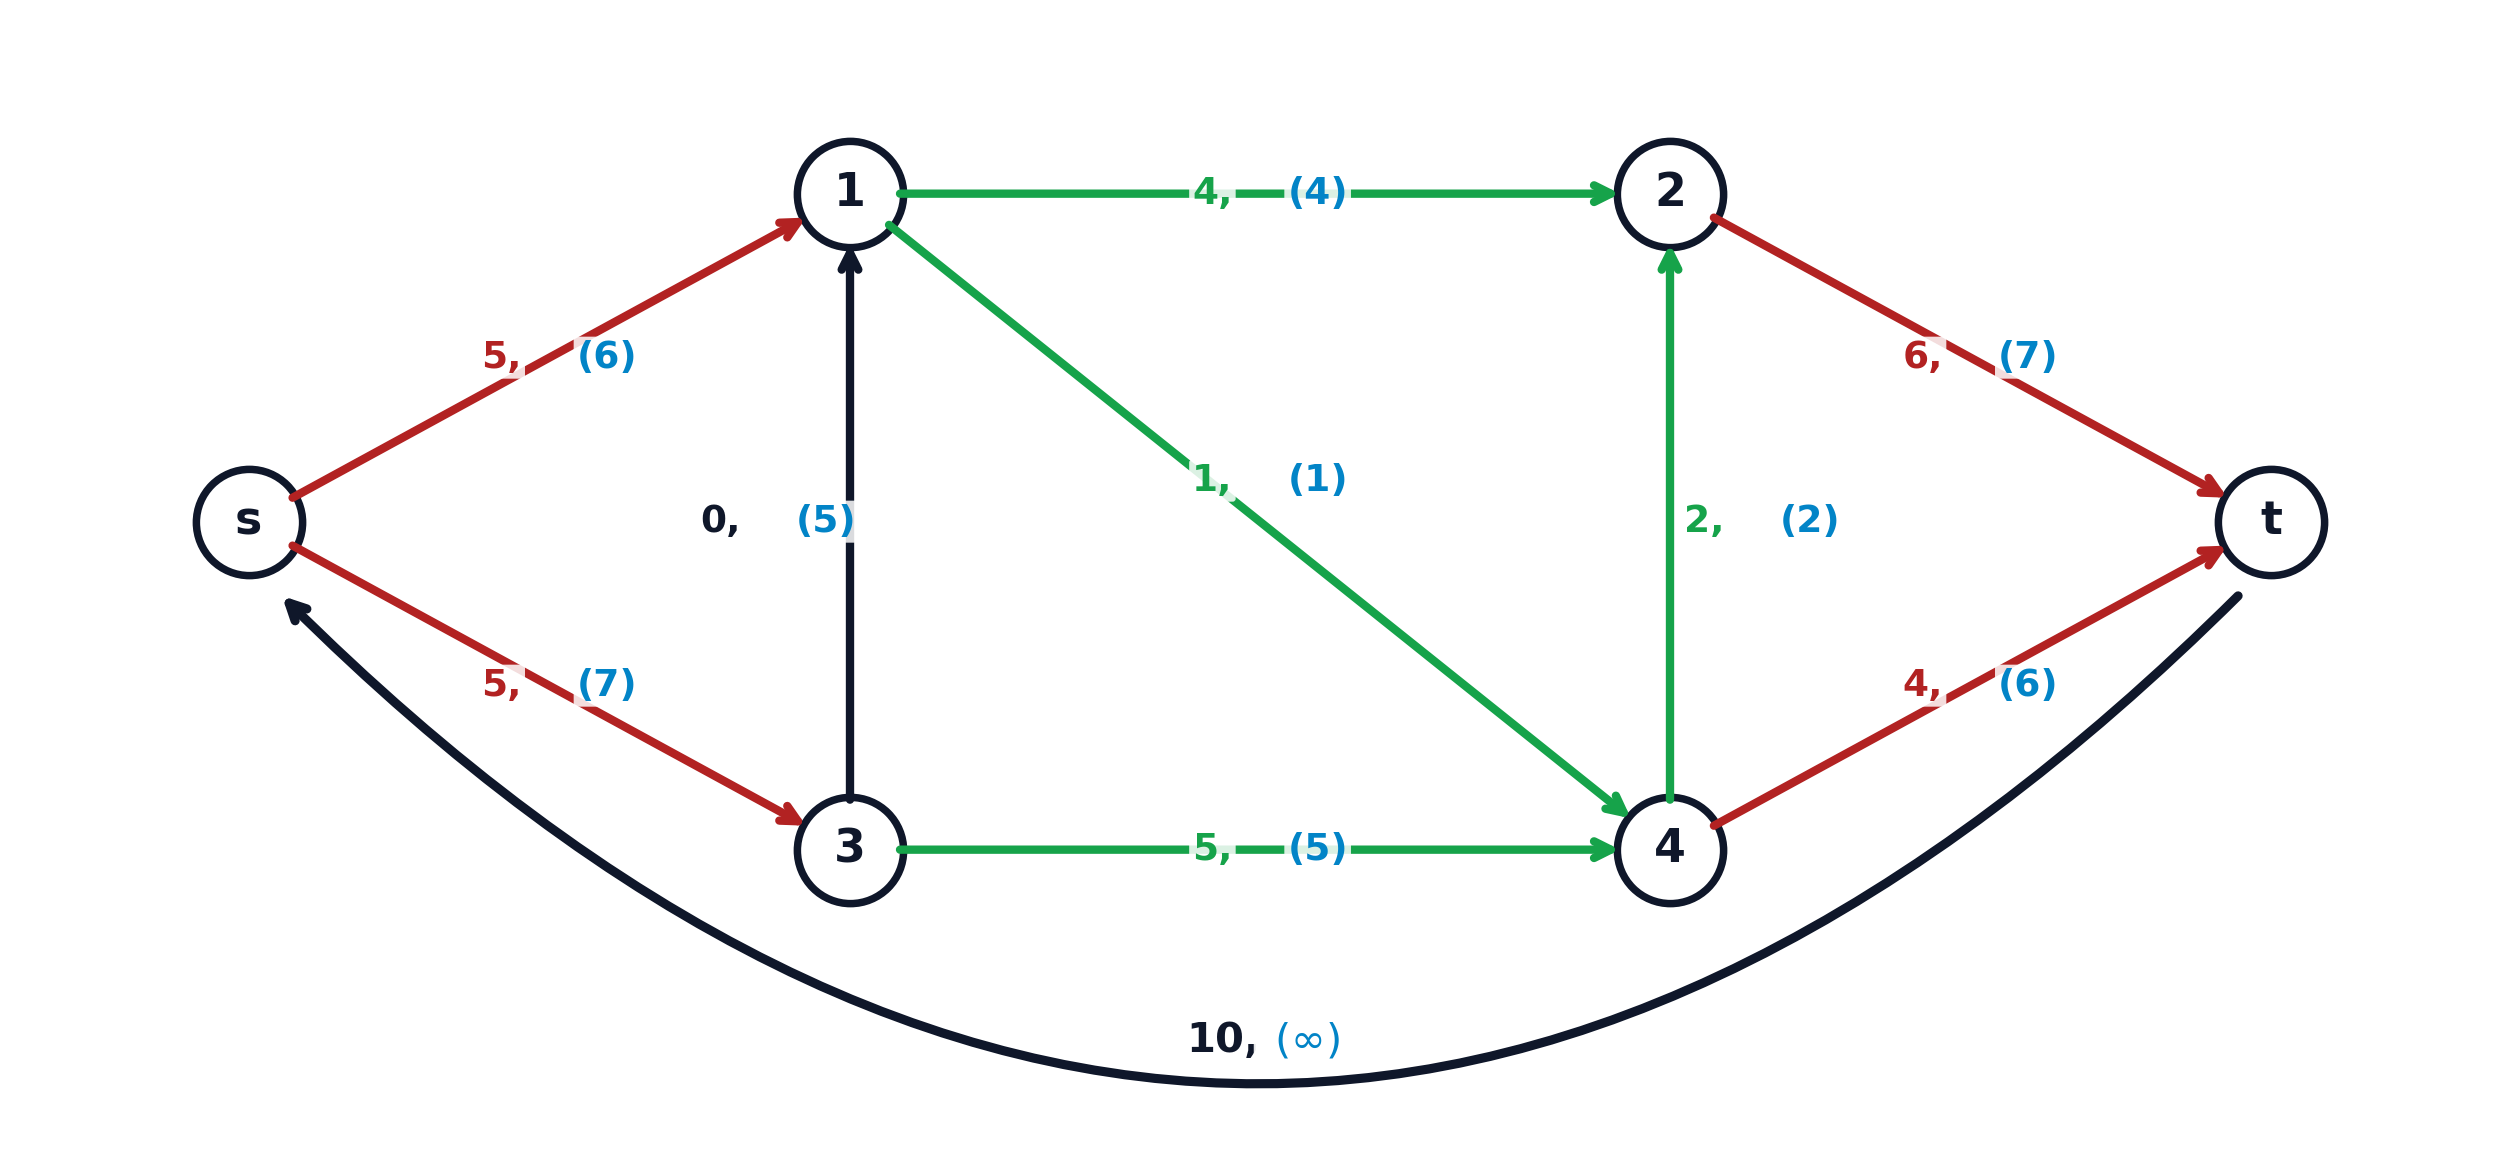
\includegraphics[width=0.75\linewidth,height=\textheight,keepaspectratio]{images/minty_demostracion_red59.png}

}

\caption{\label{fig-minty-demostracion-red59}Aplicación de la regla de
coloración de Minty sobre una red de transporte en flujo óptimo de valor
\(f_0 = 10\)}

\end{figure}%

\begin{enumerate}
\def\labelenumi{\arabic{enumi}.}
\setcounter{enumi}{1}
\tightlist
\item
  \textbf{Evaluación de la propagación del marcado de vértices}:

  \begin{itemize}
  \tightlist
  \item
    Iniciamos marcando el origen: \(S = \{s\}\).
  \item
    Desde \(s\), a través de los arcos rojos \((s,1)\) y \((s,3)\),
    marcamos los nodos \(1\) y \(3\): \(S = \{s, 1, 3\}\).
  \item
    Desde los nodos marcados \(1\) y \(3\), los arcos salientes
    \((1,2)\), \((1,4)\) y \((3,4)\) son verdes (no permiten marcar
    \(2\) ni \(4\)), y los arcos entrantes a \(1\) y \(3\) son negros
    (no permiten marcar nodos adicionales). El marcado finaliza con
    \(S = \{s, 1, 3\}\).
  \item
    Dado que el sumidero \(t \notin S\), el proceso no encuentra ningún
    camino incremental a \(t\). El conjunto de nodos marcados
    \(N = \{s, 1, 3\}\) define un \((s, t)\)-corte cuyos arcos salientes
    \(w^+(N) = \{(1,2), (1,4), (3,4)\}\) son todos verdes y suman
    capacidad \(C(w^+(N)) = 4 + 1 + 5 = 10 = f_0\), verificando la
    optimalidad.
  \end{itemize}
\item
  \textbf{Análisis de sensibilidad ante modificaciones de capacidad}: Si
  la capacidad del arco \((1,4)\) se eleva a \(c_{14} = 6\) mientras el
  flujo se mantiene en \(f_{14} = 1\) (como se ilustra en la
  Figura~\ref{fig-minty-demostracion-red62}), el arco \((1,4)\) pasa de
  verde a \textbf{rojo} (\(0 < 1 < 6\)). Al ser rojo, la propagación
  desde el nodo marcado \(1\) permite marcar el nodo \(4\), y desde
  \(4\), el arco rojo \((4,t)\) permite marcar finalmente el sumidero
  \(t\). Alcanzar el nodo \(t\) indica que el flujo \(f_0 = 10\) ya no
  es óptimo y permite enviar flujo adicional a través de la cadena
  incremental \(s \to 1 \to 4 \to t\).
\end{enumerate}

\begin{figure}[H]

\centering{

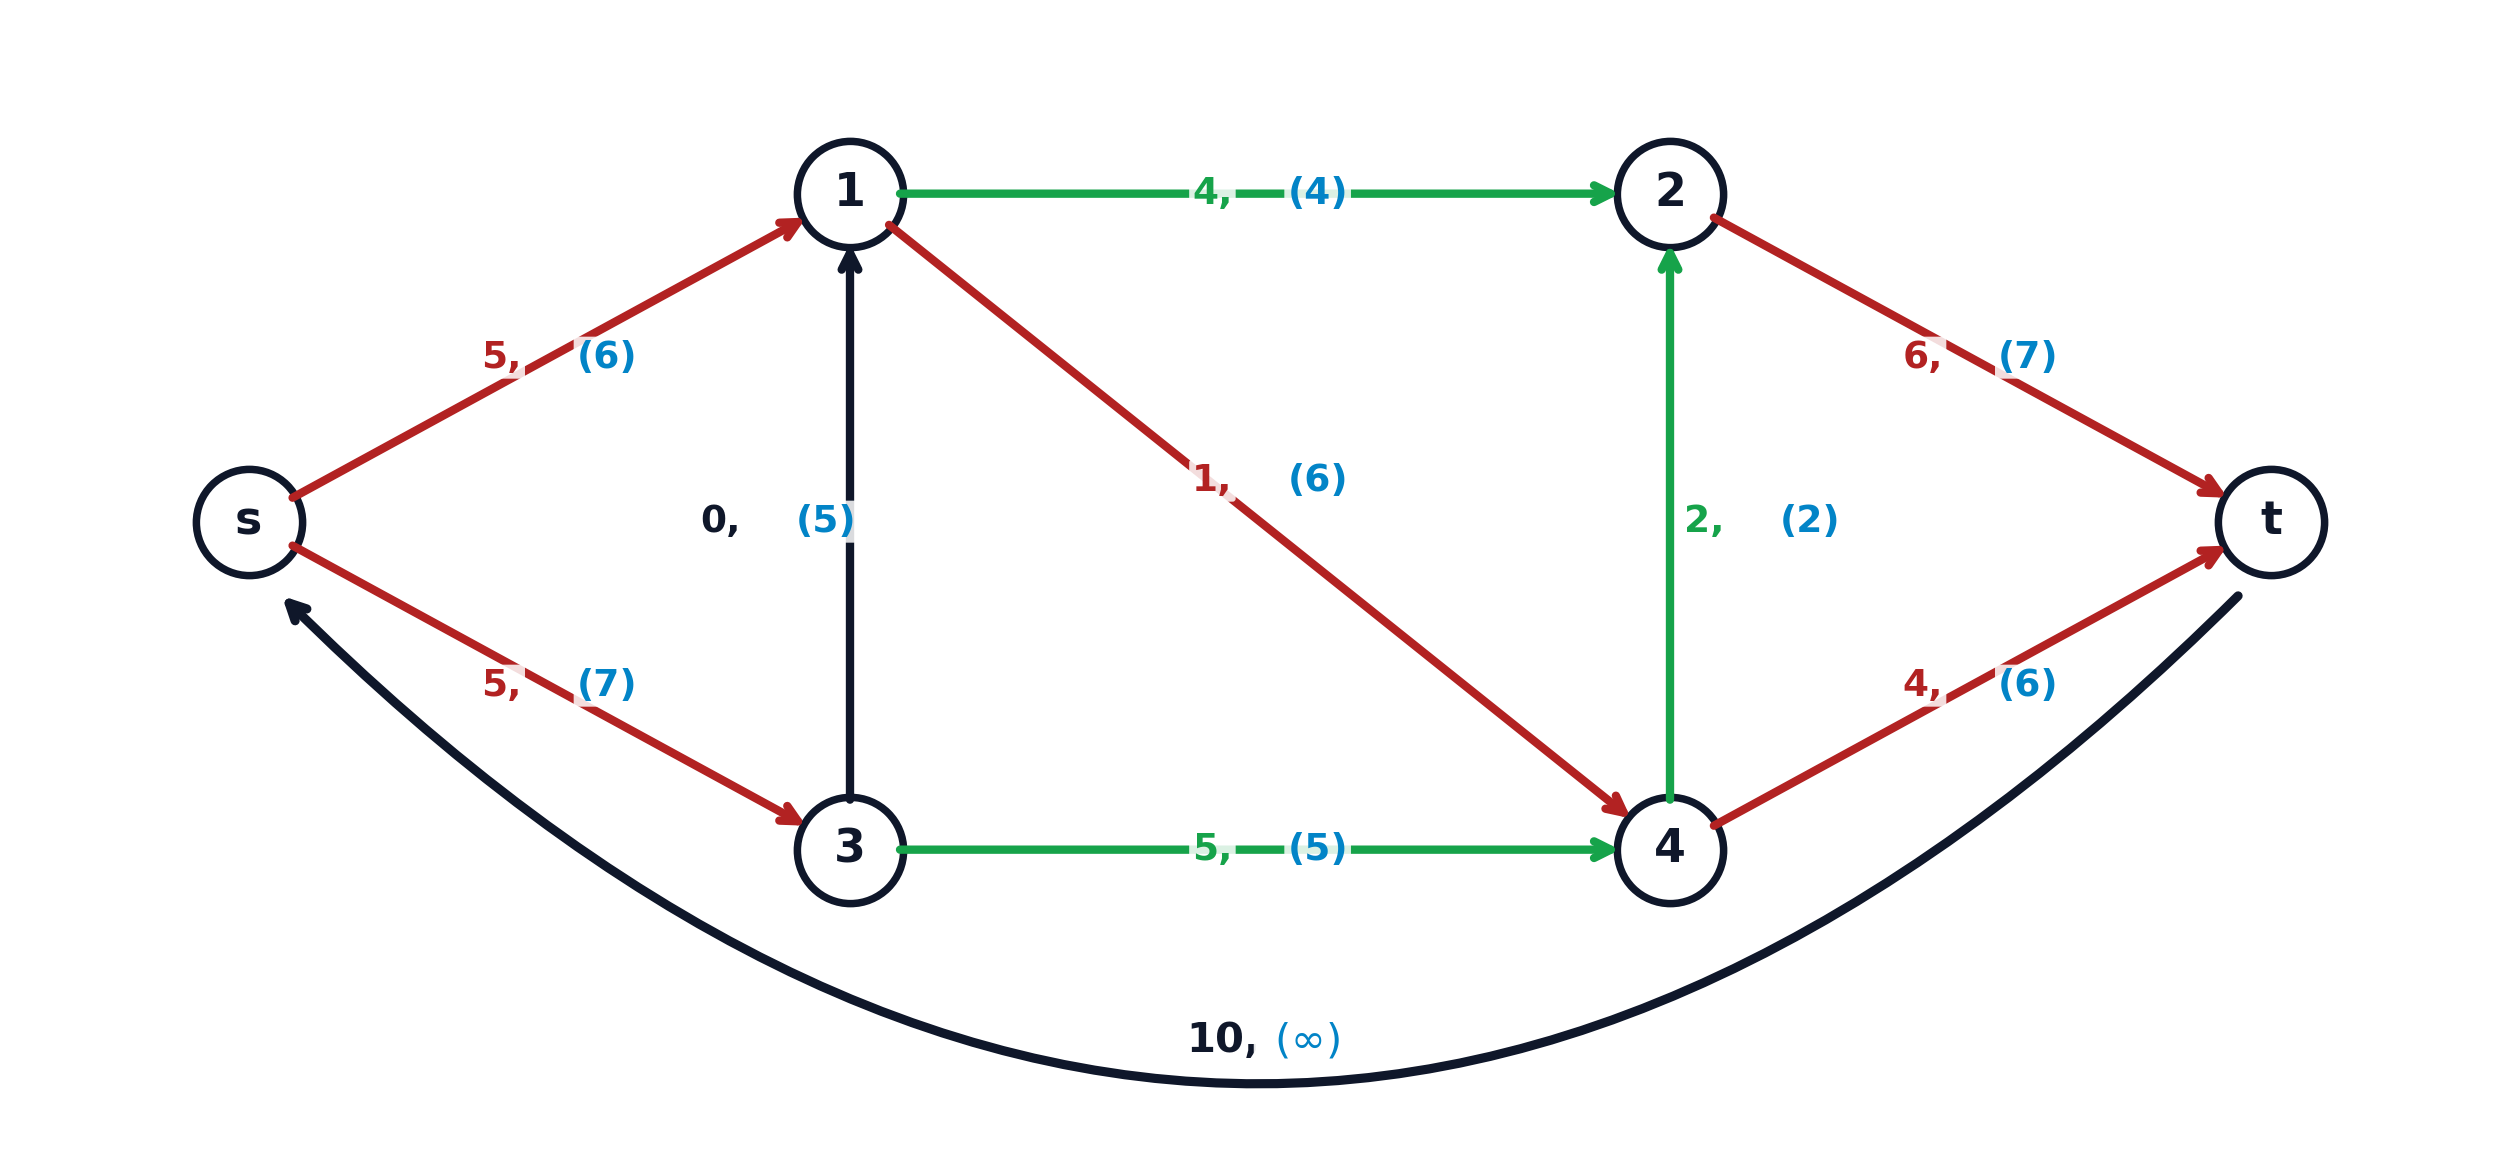
\includegraphics[width=0.75\linewidth,height=\textheight,keepaspectratio]{images/minty_demostracion_red62.png}

}

\caption{\label{fig-minty-demostracion-red62}Evaluación del marcado de
vértices cuando una modificación de capacidad convierte un arco en rojo
y habilita el marcado del sumidero \(t\)}

\end{figure}%

\end{tcolorbox}

\subsection{Algoritmo de
Ford-Fulkerson}\label{algoritmo-de-ford-fulkerson}

El \textbf{algoritmo de Ford-Fulkerson}, publicado en 1956 por L. R.
Ford (1927-2017) y D. R. Fulkerson (1924-1976), es el método clásico
fundamental de la teoría de flujos. Se conoce también como
\textbf{algoritmo del camino de aumento}, ya que su idea principal
consiste en aumentar progresivamente el caudal de los flujos a lo largo
de caminos orientados desde la fuente \(s\) hasta el sumidero \(t\).

Aplicando la regla de coloración de arcos vista en la demostración del
Teorema de Ford-Fulkerson y etiquetando/marcando arcos según el Lema de
Minty, es posible determinar de forma directa si un flujo es óptimo o
no. Además, en caso de que no sea óptimo, este procedimiento identifica
explícitamente un ciclo o camino por el que es posible incrementar el
flujo circulante.

\begin{tcolorbox}[enhanced jigsaw, toprule=.15mm, opacitybacktitle=0.6, coltitle=black, colbacktitle=quarto-callout-note-color!10!white, title=\textcolor{quarto-callout-note-color}{\faInfo}\hspace{0.5em}{Definición: Grafo incremental (Red residual)}, arc=.35mm, rightrule=.15mm, toptitle=1mm, breakable, bottomtitle=1mm, titlerule=0mm, colback=white, opacityback=0, leftrule=.75mm, colframe=quarto-callout-note-color-frame, left=2mm, bottomrule=.15mm]

Planteado un problema de flujo máximo de \(s\) a \(t\) en la red de
transporte \((G = (V, U), \mathbf{c})\) y dado un flujo compatible
\(\mathbf{f}\), se define el \textbf{grafo incremental} (o \textbf{red
residual}) \(G(\mathbf{f}) = (V, U(\mathbf{f}))\) como el digrafo en el
que el conjunto de arcos \(U(\mathbf{f})\) se construye para todo
\(u = (i, j) \in U\) según:

\[
\begin{cases}
u^+ = (i, j) \in U(\mathbf{f}) \text{ con peso } \ell_{u^+} = c_u - f_u, & \text{si } f_u < c_u \\
u^- = (j, i) \in U(\mathbf{f}) \text{ con peso } \ell_{u^-} = f_u, & \text{si } f_u > 0
\end{cases}
\]

\begin{itemize}
\tightlist
\item
  \textbf{Arcos directos \(u^+\)}: Se añade un arco al grafo incremental
  en el mismo sentido que el arco de la red cuando el flujo del arco en
  la red se puede incrementar (\(f_u < c_u\)). Se le asocia un peso
  \(\ell_{u^+} = c_u - f_u\).
\item
  \textbf{Arcos inversos \(u^-\)}: Se añade un arco al grafo incremental
  en sentido contrario al del arco de la red cuando el flujo del arco en
  la red se puede reducir (\(f_u > 0\)). Se le asocia un peso
  \(\ell_{u^-} = f_u\).
\end{itemize}

\emph{Propiedades}:

\begin{enumerate}
\def\labelenumi{\arabic{enumi}.}
\tightlist
\item
  Estas operaciones no son excluyentes: si un arco satisface
  \(0 < f_u < c_u\), genera tanto un arco directo \(u^+\) como un arco
  inverso \(u^-\) en \(G(\mathbf{f})\).
\item
  El arco ficticio de retorno \(u_0 = (t, s)\) \textbf{no se incluye} en
  el grafo incremental.
\item
  A cada arco de \(U(\mathbf{f})\) se le asocia una cantidad \(\ell_u\)
  que representa el flujo máximo que admite el arco en cuestión.
\end{enumerate}

\end{tcolorbox}

\begin{tcolorbox}[enhanced jigsaw, toprule=.15mm, opacitybacktitle=0.6, coltitle=black, colbacktitle=quarto-callout-tip-color!10!white, title=\textcolor{quarto-callout-tip-color}{\faLightbulb}\hspace{0.5em}{Ejemplo: Construcción del grafo incremental asociado a una red de
transporte}, arc=.35mm, rightrule=.15mm, toptitle=1mm, breakable, bottomtitle=1mm, titlerule=0mm, colback=white, opacityback=0, leftrule=.75mm, colframe=quarto-callout-tip-color-frame, left=2mm, bottomrule=.15mm]

Considérese la red de transporte de 6 nodos \(V = \{s, 2, 3, 4, 5, t\}\)
ilustrada en la Figura~\ref{fig-red-incremental-ejemplo} (izquierda),
equipada con un flujo compatible \(\mathbf{f}\) de valor \(f_0 = 3\).

Para construir su correspondiente grafo incremental \(G(\mathbf{f})\)
(derecha):

\begin{itemize}
\tightlist
\item
  Por cada arco con \(f_u < c_u\) (por ejemplo, \((s, 2)\) con
  \(f=1, c=3\)), añadimos el arco directo \((s, 2)\) con peso
  \(\ell = 3 - 1 = 2\).
\item
  Por cada arco con \(f_u > 0\) (por ejemplo, \((s, 2)\) con \(f=1\)),
  añadimos el arco inverso \((2, s)\) con peso \(\ell = 1\).
\item
  Los arcos a capacidad máxima (\(f_u = c_u\), como \((s, 3)\) con
  \(2,(2)\)) solo generan arco inverso \((3, s)\) con peso \(\ell = 2\).
\item
  Los arcos con flujo nulo (\(f_u = 0\), como \((3, 2)\) con \(0,(1)\))
  solo generan arco directo \((3, 2)\) con peso \(\ell = 1\).
\end{itemize}

\begin{figure}[H]

\centering{

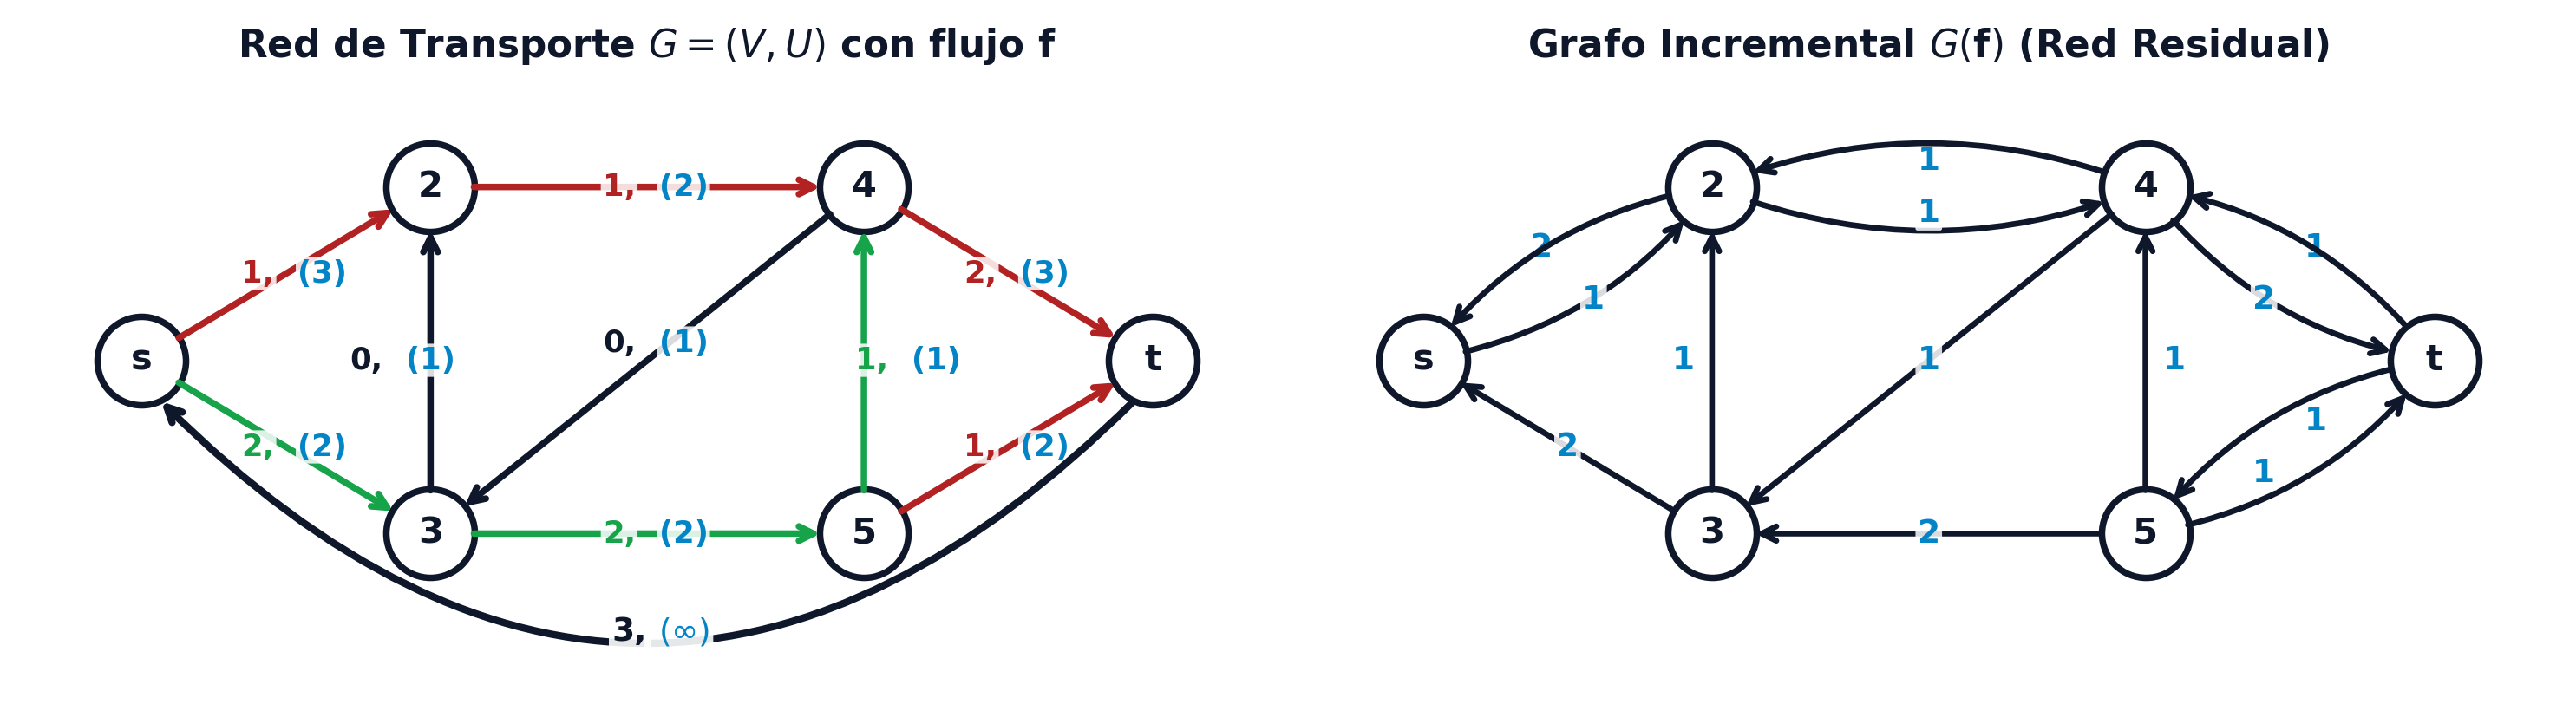
\includegraphics[width=0.95\linewidth,height=\textheight,keepaspectratio]{images/red_incremental_ejemplo.png}

}

\caption{\label{fig-red-incremental-ejemplo}Transformación de una red de
transporte con flujo \(\mathbf{f}\) (izquierda) a su correspondiente
grafo incremental \(G(\mathbf{f})\) con pesos residuales \(\ell_u\)
(derecha)}

\end{figure}%

\end{tcolorbox}

La clave del algoritmo radica en que un flujo compatible \(\mathbf{f}\)
admite un incremento en su valor \(f_0\) \textbf{si y sólo si existe un
camino orientado \(\mu[s, t]\) desde la fuente \(s\) hasta el sumidero
\(t\) en el grafo incremental \(G(\mathbf{f})\)}.

El procedimiento sistemático para resolver cualquier problema de flujo
máximo mediante la red residual se resume en la siguiente especificación
paso a paso:

\begin{tcolorbox}[enhanced jigsaw, toprule=.15mm, opacitybacktitle=0.6, coltitle=black, colbacktitle=quarto-callout-note-color!10!white, title=\textcolor{quarto-callout-note-color}{\faInfo}\hspace{0.5em}{Esquema: Algoritmo de Ford-Fulkerson por Red Incremental}, arc=.35mm, rightrule=.15mm, toptitle=1mm, breakable, bottomtitle=1mm, titlerule=0mm, colback=white, opacityback=0, leftrule=.75mm, colframe=quarto-callout-note-color-frame, left=2mm, bottomrule=.15mm]

\begin{itemize}
\item
  \textbf{Paso 1 (Inicialización)}: Hacer \(k = 0\). Determinar un flujo
  inicial compatible \(\mathbf{f}^0 = (f_0^0, f_1^0, \dots, f_m^0)^T\)
  (típicamente el flujo trivial nulo \(\mathbf{f}^0 = \mathbf{0}\)).
\item
  \textbf{Paso 2 (Construcción y Búsqueda)}: Definir la red incremental
  \(G(\mathbf{f}^k) = (V, U(\mathbf{f}^k))\). Buscar un camino orientado
  \(\mu^k\) desde \(s\) hasta \(t\) en \(G(\mathbf{f}^k)\).

  \begin{itemize}
  \tightlist
  \item
    \textbf{Si no existe el camino}: \textbf{PARAR}. El flujo actual
    \(\mathbf{f}^k\) es \textbf{óptimo} (y el conjunto de nodos
    alcanzables desde \(s\) en \(G(\mathbf{f}^k)\) define el
    \textbf{corte de capacidad mínima}).
  \item
    \textbf{En caso contrario}: Ir al Paso 3.
  \end{itemize}
\item
  \textbf{Paso 3 (Aumento de Flujo y Actualización)}: Calcular la
  capacidad del cuello de botella en la cadena incremental:
  \[ \epsilon^k = \min \{\ell_u \mid u \in \mu^k, \, u \in U(\mathbf{f}^k)\} \]
  Para cada arco \(u \in U\) de la red de transporte original: \[
  f_u^{k+1} = \begin{cases}
  f_u^k + \epsilon^k, & \text{si } u \in \mu^k(+) \text{ (arco directo en la red)} \\
  f_u^k - \epsilon^k, & \text{si } u \in \mu^k(-) \text{ (arco inverso en la red)} \\
  f_u^k, & \text{si } u \notin \mu^k(+) \cup \mu^k(-) \text{ y } u \neq (t, s)
  \end{cases}
  \] E incrementar el valor del flujo circulante por el arco ficticio de
  retorno \(u_0 = (t, s)\): \[ f_0^{k+1} = f_0^k + \epsilon^k \] Hacer
  \(k \leftarrow k + 1\) y regresar al Paso 2.
\end{itemize}

\end{tcolorbox}

\begin{tcolorbox}[enhanced jigsaw, toprule=.15mm, opacitybacktitle=0.6, coltitle=black, colbacktitle=quarto-callout-tip-color!10!white, title=\textcolor{quarto-callout-tip-color}{\faLightbulb}\hspace{0.5em}{Ejemplo: Resolución completa paso a paso del Algoritmo de Ford-Fulkerson
desde flujo nulo}, arc=.35mm, rightrule=.15mm, toptitle=1mm, breakable, bottomtitle=1mm, titlerule=0mm, colback=white, opacityback=0, leftrule=.75mm, colframe=quarto-callout-tip-color-frame, left=2mm, bottomrule=.15mm]

Considérese la red de 6 nodos \(V = \{s, 2, 3, 4, 5, t\}\) con fuente
\(s\), sumidero \(t\) y capacidades de arcos asociadas:

\[
c_{s2}=3, \quad c_{s3}=2, \quad c_{32}=1, \quad c_{24}=2, \quad c_{43}=1, \quad c_{35}=2, \quad c_{54}=1, \quad c_{4t}=3, \quad c_{5t}=2
\]

Se aplica el algoritmo de Ford-Fulkerson por red incremental partiendo
del flujo trivial nulo \(\mathbf{f}^0 = \mathbf{0}\). La traza completa
de la resolución mediante la red residual y el flujo resultante se
ilustra paso a paso en la
\textbf{?@fig-ford-fulkerson-completo-animado}:

\textbf{Iteración 1 (\(k=0\))}:

\begin{itemize}
\item
  \textbf{Paso 1 (Inicialización)}: Flujos iniciales \(f_u^0 = 0\) para
  todo arco \(u \in U\), con caudal de retorno \(f_0^0 = 0\).
\item
  \textbf{Paso 2 (Red Incremental \(G(\mathbf{f}^0)\))}: Como todos los
  flujos son nulos, la red residual contiene únicamente los arcos
  directos \(u^+\) con capacidades residuales \(\ell_{u^+} = c_u\).
\item
  \textbf{Búsqueda de Camino Aumentante}: Se detecta la trayectoria
  orientada \(\mu_1 = (s \to 2 \to 4 \to t)\).
\item
  \textbf{Cálculo del Cuello de Botella}:
  \[ \epsilon_1 = \min \{\ell_{s2}, \ell_{24}, \ell_{4t}\} = \min \{3, 2, 3\} = 2 \]
\item
  \textbf{Paso 3 (Actualización de Flujos \(\mathbf{f}^1\))}:

  \begin{itemize}
  \tightlist
  \item
    \(f_{s2}^1 = 0 + 2 = 2\)
  \item
    \(f_{24}^1 = 0 + 2 = 2\) (el arco \((2,4)\) queda \textbf{saturado},
    pasando a verde)
  \item
    \(f_{4t}^1 = 0 + 2 = 2\)
  \item
    Caudal circulante de retorno: \(f_0^1 = 0 + 2 = 2\).
  \end{itemize}
\end{itemize}

\textbf{Iteración 2 (\(k=1\))}:

\begin{itemize}
\item
  \textbf{Paso 2 (Red Incremental \(G(\mathbf{f}^1)\))}:

  \begin{itemize}
  \tightlist
  \item
    Al estar saturado el arco \((2,4)\), en \(G(\mathbf{f}^1)\) solo
    existe el arco inverso \((4,2)\) con peso \(\ell = 2\).
  \item
    El arco \((s,2)\) admite incremento \(\ell = 3 - 2 = 1\) e inverso
    \((2,s)\) con peso \(\ell = 2\).
  \end{itemize}
\item
  \textbf{Búsqueda de Camino Aumentante}: Se detecta la trayectoria
  orientada \(\mu_2 = (s \to 3 \to 5 \to t)\).
\item
  \textbf{Cálculo del Cuello de Botella}:
  \[ \epsilon_2 = \min \{\ell_{s3}, \ell_{35}, \ell_{5t}\} = \min \{2, 2, 2\} = 2 \]
\item
  \textbf{Paso 3 (Actualización de Flujos \(\mathbf{f}^2\))}:

  \begin{itemize}
  \tightlist
  \item
    \(f_{s3}^2 = 0 + 2 = 2\) (arco \textbf{saturado}, verde)
  \item
    \(f_{35}^2 = 0 + 2 = 2\) (arco \textbf{saturado}, verde)
  \item
    \(f_{5t}^2 = 0 + 2 = 2\) (arco \textbf{saturado}, verde)
  \item
    Caudal circulante de retorno: \(f_0^2 = 2 + 2 = 4\).
  \end{itemize}
\end{itemize}

\textbf{Iteración 3 (\(k=2\)) y Criterio de Parada}:

\begin{itemize}
\tightlist
\item
  \textbf{Paso 2 (Red Incremental \(G(\mathbf{f}^2)\))}:

  \begin{itemize}
  \tightlist
  \item
    Al construir \(G(\mathbf{f}^2)\), todos los arcos salientes desde la
    fuente \(s\) a través de \(3\) están saturados. El único nodo
    alcanzable desde \(s\) mediante caminos orientados en
    \(G(\mathbf{f}^2)\) es el nodo \(2\).
  \item
    \textbf{Conclusión de Parada}: No existe ningún camino orientado
    desde \(s\) hasta \(t\) en la red residual \(G(\mathbf{f}^2)\). Por
    tanto, el flujo \(\mathbf{f}^2\) es el \textbf{flujo máximo} con
    valor \(f_0^* = 4\).
  \end{itemize}
\end{itemize}

\textbf{Corte de Capacidad Mínima Resultante}:

\begin{itemize}
\tightlist
\item
  El subconjunto de nodos alcanzables desde la fuente \(s\) en la red
  residual final es \(N = \{s, 2\}\).
\item
  El corte de capacidad mínima asociado es
  \(w^+(N) = \{(s,3), (2,4)\}\).
\item
  Capacidad del corte:
  \[ C(w^+(N)) = c_{s3} + c_{24} = 2 + 2 = 4 = f_0^* \]
\end{itemize}

\textbf{Código de colores de los arcos y nodos en la representación
gráfica}:

\begin{itemize}
\tightlist
\item
  \textbf{Arcos en naranja (\(\textcolor{orange}{\rightarrow}\))}:
  Indican los arcos que integran el \textbf{camino aumentante}
  seleccionado en la iteración actual.
\item
  \textbf{Arcos en verde (\(\textcolor{forestgreen}{\rightarrow}\))}:
  Indican arcos que han quedado \textbf{saturados} a su capacidad máxima
  (\(f_u = c_u\)).
\item
  \textbf{Arcos en rojo (\(\textcolor{firebrick}{\rightarrow}\))}:
  Indican arcos por los que circula un \textbf{flujo parcial no nulo}
  (\(0 < f_u < c_u\)).
\item
  \textbf{Arcos en negro (\(\rightarrow\))}: Indican arcos con
  \textbf{flujo nulo} (\(f_u = 0\)) o no transitados.
\item
  \textbf{Arcos/Nodos en azul (\(\textcolor{blue}{\rightarrow}\))}: En
  la iteración de parada, destacan los nodos alcanzables
  \(N = \{s, 2\}\) y los arcos que componen el \textbf{corte de
  capacidad mínima} \(w^+(N)\).
\end{itemize}

\end{tcolorbox}

Una vez analizada la fundamentación teórica y la traza explícita
mediante la red residual \(G(\mathbf{f})\), en la práctica manual o
computacional directa resulta ineficiente reconstruir e ilustrar la
estructura del grafo incremental en cada iteración. Por esta razón, Ford
y Fulkerson diseñaron un procedimiento simplificado de implementación
directa denominado \textbf{algoritmo por etiquetado de vértices}, que
opera sobre los nodos de la red original mediante marcas dinámicas.

\subsection{Algoritmo de Ford-Fulkerson por etiquetado de
vértices}\label{algoritmo-de-ford-fulkerson-por-etiquetado-de-vuxe9rtices}

El algoritmo de Ford-Fulkerson se puede plantear de forma más sencilla e
intuitiva sin necesidad de construir explícitamente el grafo incremental
\(G(\mathbf{f})\) en cada iteración. Para ello, se emplea una
\textbf{regla de etiquetado dinámico de vértices} que opera directamente
sobre la red de transporte original.

Inicialmente se asigna una etiqueta a la fuente \(s\),
\(\text{Etiqueta}(s) = (\text{–}, \, \textcolor{dodgerblue}{\delta_s = +\infty})\),
y paso a paso se propagan marcas y etiquetas al resto de vértices no
explorados.

\begin{tcolorbox}[enhanced jigsaw, toprule=.15mm, opacitybacktitle=0.6, coltitle=black, colbacktitle=quarto-callout-note-color!10!white, title=\textcolor{quarto-callout-note-color}{\faInfo}\hspace{0.5em}{Definición: Estructura de las etiquetas de vértices}, arc=.35mm, rightrule=.15mm, toptitle=1mm, breakable, bottomtitle=1mm, titlerule=0mm, colback=white, opacityback=0, leftrule=.75mm, colframe=quarto-callout-note-color-frame, left=2mm, bottomrule=.15mm]

La etiqueta asignada a un nodo \(j\) presenta dos componentes
diferenciadas:

\[
\text{Etiqueta}(j) = (\textcolor{darkgray}{\pm i}, \, \textcolor{dodgerblue}{\delta_j})
\]

\begin{enumerate}
\def\labelenumi{\arabic{enumi}.}
\tightlist
\item
  \textbf{Procedencia (\(\textcolor{darkgray}{\pm i}\))}: Indica el nodo
  antecedente \(i\) (ya etiquetado) que se utiliza para etiquetar al
  nodo \(j\). El signo del antecedente determina la orientación del
  tránsito:

  \begin{itemize}
  \tightlist
  \item
    \textbf{\(\textcolor{forestgreen}{+i}\) (Arco directo \((i, j)\))}:
    El arco está dirigido de \(i\) hacia \(j\) y su flujo actual es
    inferior a su capacidad (\(f_{ij} < c_{ij}\)). Permite incrementar
    flujo.
  \item
    \textbf{\(\textcolor{firebrick}{-i}\) (Arco inverso \((j, i)\))}: El
    arco está dirigido de \(j\) hacia \(i\) y su flujo actual es
    positivo (\(f_{ji} > 0\)). Permite reducir flujo.
  \end{itemize}
\item
  \textbf{Capacidad disponible (\(\textcolor{dodgerblue}{\delta_j}\))}:
  Indica el valor máximo de flujo incremental que es posible hacer
  llegar desde la fuente \(s\) hasta el nodo \(j\) a través de la cadena
  de antecedentes iniciada en \(i\).
\end{enumerate}

\end{tcolorbox}

\begin{tcolorbox}[enhanced jigsaw, toprule=.15mm, opacitybacktitle=0.6, coltitle=black, colbacktitle=quarto-callout-note-color!10!white, title=\textcolor{quarto-callout-note-color}{\faInfo}\hspace{0.5em}{Definición: Reglas formales de etiquetado}, arc=.35mm, rightrule=.15mm, toptitle=1mm, breakable, bottomtitle=1mm, titlerule=0mm, colback=white, opacityback=0, leftrule=.75mm, colframe=quarto-callout-note-color-frame, left=2mm, bottomrule=.15mm]

Sea \(i \in V\) un nodo previamente etiquetado con etiqueta
\((\cdot, \, \textcolor{dodgerblue}{\delta_i})\) y sea \(j \in V\) un
nodo adyacente aún \textbf{no etiquetado}:

\begin{enumerate}
\def\labelenumi{\arabic{enumi}.}
\item
  \textbf{Regla 1 (Arco Directo \((i, j) \in U\))}: Si
  \(f_{ij} < c_{ij}\), se etiqueta el nodo \(j\) como
  \((\textcolor{forestgreen}{+i}, \, \textcolor{dodgerblue}{\delta_j})\),
  donde el cuello de botella se actualiza como:
  \[ \textcolor{dodgerblue}{\delta_j} = \min \left\{ \textcolor{dodgerblue}{\delta_i}, \, c_{ij} - f_{ij} \right\} \]
\item
  \textbf{Regla 2 (Arco Inverso \((j, i) \in U\))}: Si \(f_{ji} > 0\),
  se etiqueta el nodo \(j\) como
  \((\textcolor{firebrick}{-i}, \, \textcolor{dodgerblue}{\delta_j})\),
  donde la capacidad de reducción se calcula como:
  \[ \textcolor{dodgerblue}{\delta_j} = \min \left\{ \textcolor{dodgerblue}{\delta_i}, \, f_{ji} \right\} \]
\end{enumerate}

Un vértice se considera \textbf{explorado} cuando está etiquetado o bien
no es posible etiquetar a ninguno de sus nodos adyacentes no
etiquetados.

\end{tcolorbox}

\begin{figure}

\centering{

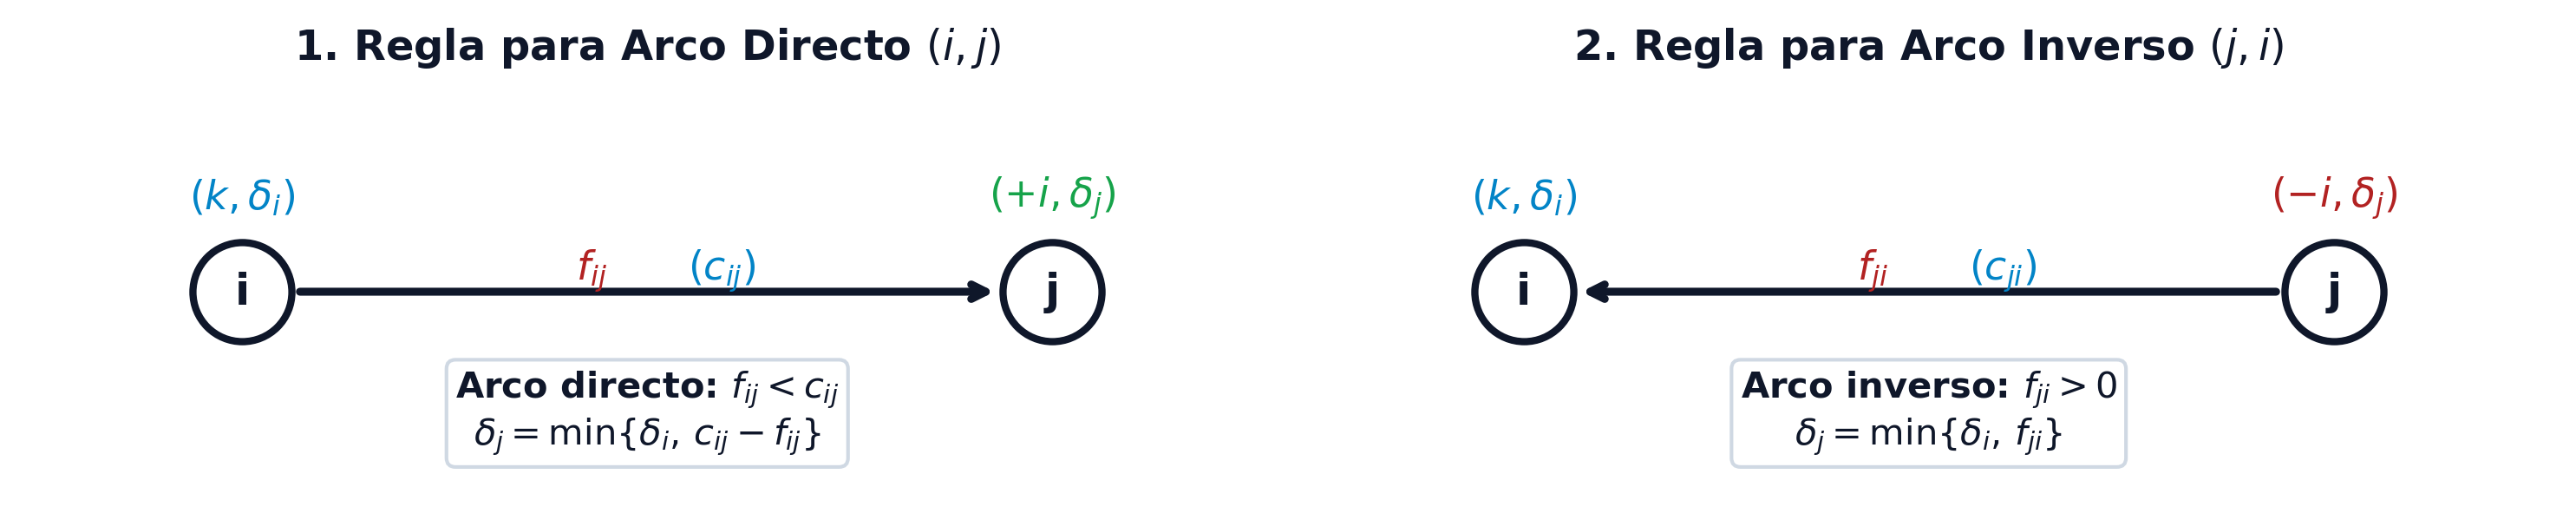
\includegraphics[width=0.85\linewidth,height=\textheight,keepaspectratio]{images/reglas_etiquetado_ford_fulkerson.png}

}

\caption{\label{fig-reglas-etiquetado-ford-fulkerson}Reglas de
etiquetado de vértices en el algoritmo de Ford-Fulkerson: asignación de
marcas directas \((+i, \delta_j)\) en arcos salientes (izquierda) y
marcas inversas \((-i, \delta_j)\) en arcos entrantes (derecha)}

\end{figure}%

Como se ilustra en la Figura~\ref{fig-reglas-etiquetado-ford-fulkerson},
la propagación de marcas desde la fuente \(s\) explora secuencialmente
la red:

\begin{itemize}
\tightlist
\item
  \textbf{Si al final del proceso el sumidero \(t\) resulta etiquetado}:
  Se ha alcanzado con éxito el destino a través de una cadena de aumento
  \(\mu[s, t]\). El valor de la etiqueta del sumidero
  \(\Delta = \textcolor{dodgerblue}{\delta_t}\) determina la cantidad
  exacta en la que se debe incrementar el flujo circulante \(f_0\).
\item
  \textbf{Si no es posible etiquetar el sumidero \(t\)
  (\(t \notin S\))}: \textbf{PARAR}. Se ha alcanzado el \textbf{flujo
  máximo} \(f_0^*\). El conjunto de nodos etiquetados \(N = S\) define
  de forma inmediata el \textbf{corte de capacidad mínima} \(w^+(N)\).
\end{itemize}

\begin{tcolorbox}[enhanced jigsaw, toprule=.15mm, opacitybacktitle=0.6, coltitle=black, colbacktitle=quarto-callout-note-color!10!white, title=\textcolor{quarto-callout-note-color}{\faInfo}\hspace{0.5em}{Esquema: Algoritmo de Ford-Fulkerson por Etiquetado de Vértices}, arc=.35mm, rightrule=.15mm, toptitle=1mm, breakable, bottomtitle=1mm, titlerule=0mm, colback=white, opacityback=0, leftrule=.75mm, colframe=quarto-callout-note-color-frame, left=2mm, bottomrule=.15mm]

\begin{enumerate}
\def\labelenumi{\arabic{enumi}.}
\item
  \textbf{Paso 1 (Inicialización)}: Asignar un flujo inicial compatible
  \(\mathbf{f} = \mathbf{0}\) (o un flujo compatible conocido).
  Etiquetar la fuente \(s\) con la marca inicial
  \((\text{–}, \, \textcolor{dodgerblue}{\delta_s = +\infty})\).
\item
  \textbf{Paso 2 (Evaluación de Exploración)}: ¿Todos los vértices
  etiquetados han sido totalmente explorados?

  \begin{itemize}
  \tightlist
  \item
    \textbf{SÍ}: Ir al \textbf{Paso 6}.
  \item
    \textbf{NO}: Ir al \textbf{Paso 3}.
  \end{itemize}
\item
  \textbf{Paso 3 (Propagación de Etiquetas)}: Etiquetar todos los
  vértices adyacentes posibles mediante la \textbf{Regla 1} (arcos
  directos) y la \textbf{Regla 2} (arcos inversos).
\item
  \textbf{Paso 4 (Verificación del Sumidero)}: ¿Ha sido etiquetado el
  sumidero \(t\)?

  \begin{itemize}
  \tightlist
  \item
    \textbf{SÍ}: Fijar la cantidad de aumento
    \(\Delta = \textcolor{dodgerblue}{\delta_t}\) e ir al \textbf{Paso
    5}.
  \item
    \textbf{NO}: Regresar al \textbf{Paso 2}.
  \end{itemize}
\item
  \textbf{Paso 5 (Modificación del Flujo Actual)}:

  \begin{enumerate}
  \def\labelenumii{\arabic{enumii}.}
  \item
    Inicializar el puntero de rastreo en el sumidero:
    \(k \leftarrow t\).
  \item
    Si la etiqueta del vértice \(k\) es
    \((\textcolor{forestgreen}{+i}, \, \delta_k)\), incrementar el flujo
    del arco directo: \[ f_{ik} \leftarrow f_{ik} + \Delta \]
  \item
    Si la etiqueta del vértice \(k\) es
    \((\textcolor{firebrick}{-i}, \, \delta_k)\), reducir el flujo del
    arco inverso: \[ f_{ki} \leftarrow f_{ki} - \Delta \]
  \item
    Retroceder al nodo antecedente: \(k \leftarrow i\). ¿Es \(i = s\)?

    \begin{itemize}
    \tightlist
    \item
      \textbf{SÍ}: Incrementar el flujo de retorno
      \(f_0 \leftarrow f_0 + \Delta\), borrar todas las etiquetas de los
      nodos excepto la de la fuente \(s\)
      \((\text{–}, \, \textcolor{dodgerblue}{+\infty})\) e ir al
      \textbf{Paso 2}.
    \item
      \textbf{NO}: Regresar al \textbf{Subpaso 5.2}.
    \end{itemize}
  \end{enumerate}
\item
  \textbf{Paso 6 (Optimalidad y Parada)}: El flujo actual
  \(\mathbf{f}^*\) es el \textbf{flujo máximo}. El subconjunto de
  vértices que han quedado etiquetados \(N = S\) define el \textbf{corte
  de capacidad mínima} \(w^+(N)\).
\end{enumerate}

\end{tcolorbox}

\begin{tcolorbox}[enhanced jigsaw, toprule=.15mm, opacitybacktitle=0.6, coltitle=black, colbacktitle=quarto-callout-tip-color!10!white, title=\textcolor{quarto-callout-tip-color}{\faLightbulb}\hspace{0.5em}{Ejemplo: Traza paso a paso del Algoritmo de Ford-Fulkerson por
etiquetado de vértices}, arc=.35mm, rightrule=.15mm, toptitle=1mm, breakable, bottomtitle=1mm, titlerule=0mm, colback=white, opacityback=0, leftrule=.75mm, colframe=quarto-callout-tip-color-frame, left=2mm, bottomrule=.15mm]

Considérese la red de transporte de 8 nodos
\(V = \{s, 1, 2, 3, 4, 5, 6, t\}\) equipada con las capacidades entre
paréntesis \(c_u\):

\begin{itemize}
\tightlist
\item
  \(c_{s1} = 7\), \(c_{s2} = 2\), \(c_{12} = 1\), \(c_{13} = 5\),
  \(c_{32} = 3\), \(c_{34} = 2\), \(c_{35} = 4\), \(c_{24} = 4\),
  \(c_{46} = 5\), \(c_{56} = 3\), \(c_{5t} = 3\), \(c_{6t} = 6\).
\end{itemize}

Se aplica el algoritmo de Ford-Fulkerson por etiquetado partiendo del
flujo nulo inicial \(\mathbf{f}^0 = \mathbf{0}\) (\(f_0^0 = 0\)). La
propagación dinámica de marcas, la actualización de flujos y la
delimitación del corte mínimo se ilustran paso a paso en la
\textbf{?@fig-ford-fulkerson-etiquetado-animado}:

\textbf{Iteración 1}:

\begin{itemize}
\tightlist
\item
  \textbf{Propagación de etiquetas}:

  \begin{itemize}
  \tightlist
  \item
    Etiqueta inicial en el origen:
    \(\text{Etiqueta}(s) = (\text{–}, \, \textcolor{dodgerblue}{\delta_s = +\infty})\).
  \item
    Desde \(s\): etiquetar \(1\) con
    \((\textcolor{forestgreen}{+s}, \, \textcolor{dodgerblue}{7})\) y
    \(2\) con
    \((\textcolor{forestgreen}{+s}, \, \textcolor{dodgerblue}{2})\).
  \item
    Desde \(2\): etiquetar \(4\) con
    \((\textcolor{forestgreen}{+2}, \, \textcolor{dodgerblue}{\min\{2, 4\} = 2})\).
  \item
    Desde \(4\): etiquetar \(6\) con
    \((\textcolor{forestgreen}{+4}, \, \textcolor{dodgerblue}{\min\{2, 5\} = 2})\).
  \item
    Desde \(6\): etiquetar el sumidero \(t\) con
    \((\textcolor{forestgreen}{+6}, \, \textcolor{dodgerblue}{\min\{2, 6\} = 2})\).
  \end{itemize}
\item
  \textbf{Camino aumentante}: \(\mu_1 = (s \to 2 \to 4 \to 6 \to t)\)
  con incremento de flujo
  \(\Delta_1 = \textcolor{dodgerblue}{\delta_t = 2}\).
\item
  \textbf{Actualización de flujos (\(\mathbf{f}^1\))}:

  \begin{itemize}
  \tightlist
  \item
    \(f_{s2} \leftarrow 0 + 2 = 2\) (el arco \((s,2)\) queda
    \textbf{saturado}, pasando a verde).
  \item
    \(f_{24} \leftarrow 0 + 2 = 2\), \(f_{46} \leftarrow 0 + 2 = 2\),
    \(f_{6t} \leftarrow 0 + 2 = 2\).
  \item
    Flujo total circulante de retorno: \(f_0^1 = 2\).
  \end{itemize}
\end{itemize}

\textbf{Iteración 2}:

\begin{itemize}
\tightlist
\item
  \textbf{Propagación de etiquetas}:

  \begin{itemize}
  \tightlist
  \item
    Etiqueta inicial en \(s\):
    \((\text{–}, \, \textcolor{dodgerblue}{+\infty})\). (El arco
    \((s,2)\) está saturado, no permite etiquetar \(2\)).
  \item
    Desde \(s\): etiquetar \(1\) con
    \((\textcolor{forestgreen}{+s}, \, \textcolor{dodgerblue}{7})\).
  \item
    Desde \(1\): etiquetar \(3\) con
    \((\textcolor{forestgreen}{+1}, \, \textcolor{dodgerblue}{\min\{7, 5\} = 5})\)
    y \(2\) con
    \((\textcolor{forestgreen}{+1}, \, \textcolor{dodgerblue}{\min\{7, 1\} = 1})\).
  \item
    Desde \(3\): etiquetar \(5\) con
    \((\textcolor{forestgreen}{+3}, \, \textcolor{dodgerblue}{\min\{5, 4\} = 4})\)
    y \(4\) con
    \((\textcolor{forestgreen}{+3}, \, \textcolor{dodgerblue}{\min\{5, 2\} = 2})\).
  \item
    Desde \(5\): etiquetar el sumidero \(t\) con
    \((\textcolor{forestgreen}{+5}, \, \textcolor{dodgerblue}{\min\{4, 3\} = 3})\).
  \end{itemize}
\item
  \textbf{Camino aumentante}: \(\mu_2 = (s \to 1 \to 3 \to 5 \to t)\)
  con incremento de flujo
  \(\Delta_2 = \textcolor{dodgerblue}{\delta_t = 3}\).
\item
  \textbf{Actualización de flujos (\(\mathbf{f}^2\))}:

  \begin{itemize}
  \tightlist
  \item
    \(f_{s1} \leftarrow 0 + 3 = 3\), \(f_{13} \leftarrow 0 + 3 = 3\),
    \(f_{35} \leftarrow 0 + 3 = 3\).
  \item
    \(f_{5t} \leftarrow 0 + 3 = 3\) (el arco \((5,t)\) queda
    \textbf{saturado}, pasando a verde).
  \item
    Flujo total circulante de retorno: \(f_0^2 = 2 + 3 = 5\).
  \end{itemize}
\end{itemize}

\textbf{Iteración 5}:

\begin{itemize}
\tightlist
\item
  \textbf{Propagación de etiquetas}:

  \begin{itemize}
  \tightlist
  \item
    Etiqueta inicial en \(s\):
    \((\text{–}, \, \textcolor{dodgerblue}{+\infty})\).
  \item
    Desde \(s\): el arco \((s,2)\) está saturado
    (\(f_{s2} = 2 = c_{s2}\)). Etiquetar \(1\) con
    \((\textcolor{forestgreen}{+s}, \, \textcolor{dodgerblue}{7 - 5 = 2})\).
  \item
    Desde \(1\): el arco \((1,3)\) está saturado
    (\(f_{13} = 5 = c_{13}\)). Mediante \((1,2)\) etiquetamos \(2\) con
    \((\textcolor{forestgreen}{+1}, \, \textcolor{dodgerblue}{\min\{2, 1\} = 1})\).
  \item
    Desde \(2\): mediante \((2,4)\) etiquetamos \(4\) con
    \((\textcolor{forestgreen}{+2}, \, \textcolor{dodgerblue}{\min\{1, 4 - 2\} = 1})\).
  \item
    Desde \(4\): etiquetar \(6\) con
    \((\textcolor{forestgreen}{+4}, \, \textcolor{dodgerblue}{\min\{1, 5 - 3\} = 1})\).
  \item
    Desde \(6\): etiquetar el sumidero \(t\) con
    \((\textcolor{forestgreen}{+6}, \, \textcolor{dodgerblue}{\min\{1, 6 - 4\} = 1})\).
  \end{itemize}
\item
  \textbf{Camino aumentante}:
  \(\mu_5 = (s \to 1 \to 2 \to 4 \to 6 \to t)\) con incremento de flujo
  \(\Delta_5 = \textcolor{dodgerblue}{\delta_t = 1}\).
\item
  \textbf{Actualización de flujos (\(\mathbf{f}^5\))}:

  \begin{itemize}
  \tightlist
  \item
    \(f_{s1} \leftarrow 5 + 1 = 6\).
  \item
    \(f_{12} \leftarrow 0 + 1 = 1\) (el arco \((1,2)\) queda
    \textbf{saturado}, pasando a verde).
  \item
    \(f_{24} \leftarrow 2 + 1 = 3\), \(f_{46} \leftarrow 3 + 1 = 4\),
    \(f_{6t} \leftarrow 4 + 1 = 5\).
  \item
    Flujo total circulante de retorno: \(f_0^5 = 7 + 1 = 8\).
  \end{itemize}
\end{itemize}

\textbf{Iteración 6 (Criterio de Parada)}:

\begin{itemize}
\tightlist
\item
  \textbf{Propagación de etiquetas}:

  \begin{itemize}
  \tightlist
  \item
    Etiqueta inicial en \(s\):
    \((\text{–}, \, \textcolor{dodgerblue}{+\infty})\).
  \item
    Desde \(s\): el arco \((s,2)\) está saturado. Etiquetar \(1\) con
    \((\textcolor{forestgreen}{+s}, \, \textcolor{dodgerblue}{7 - 6 = 1})\).
  \item
    Desde \(1\): el arco \((1,3)\) está saturado
    (\(f_{13} = 5 = c_{13}\)) y el arco \((1,2)\) está saturado
    (\(f_{12} = 1 = c_{12}\)). No es posible etiquetar ningún nodo
    adicional desde \(1\).
  \item
    \textbf{Fin del algoritmo}: El sumidero \(t\) \textbf{no resulta
    etiquetado} (\(t \notin S\)).
  \end{itemize}
\end{itemize}

\textbf{Solución Óptima y Corte de Capacidad Mínima}:

\begin{itemize}
\tightlist
\item
  \textbf{Valor del flujo máximo}: \(f_0^* = 8\).
\item
  \textbf{Subconjunto de vértices etiquetados}: \(N = \{s, 1\}\).
\item
  \textbf{Corte de capacidad mínima}:
  \(w^+(N) = \{(s, 2), (1, 3), (1, 2)\}\).
\item
  \textbf{Capacidad del corte}:
  \[ C(w^+(N)) = c_{s2} + c_{13} + c_{12} = 2 + 5 + 1 = 8 = f_0^* \]
\end{itemize}

\textbf{Código de colores de los arcos y nodos en la representación
gráfica}:

\begin{itemize}
\tightlist
\item
  \textbf{Arcos en naranja (\(\textcolor{orange}{\rightarrow}\))}:
  Indican los arcos que integran el \textbf{camino aumentante}
  seleccionado en la iteración actual.
\item
  \textbf{Arcos en verde (\(\textcolor{forestgreen}{\rightarrow}\))}:
  Indican arcos que han quedado \textbf{saturados} a su capacidad máxima
  (\(f_u = c_u\)).
\item
  \textbf{Arcos en rojo (\(\textcolor{firebrick}{\rightarrow}\))}:
  Indican arcos por los que circula un \textbf{flujo parcial no nulo}
  (\(0 < f_u < c_u\)).
\item
  \textbf{Arcos en negro (\(\rightarrow\))}: Indican arcos con
  \textbf{flujo nulo} (\(f_u = 0\)) o no transitados.
\item
  \textbf{Nodos en naranja (\(\textcolor{orange}{\bigcirc}\))}: En la
  iteración de parada, representan el subconjunto de nodos etiquetados
  \(N = S\) que contienen a la fuente \(s\).
\item
  \textbf{Nodos en verde (\(\textcolor{forestgreen}{\bigcirc}\))}: En la
  iteración de parada, representan el subconjunto de nodos no
  alcanzables \(V \setminus N\) que contienen al sumidero \(t\).
\item
  \textbf{Arcos en azul (\(\textcolor{blue}{\rightarrow}\))}: En la
  iteración de parada, destacan los arcos salientes que componen el
  \textbf{corte de capacidad mínima} \(w^+(N)\).
\end{itemize}

\end{tcolorbox}

La caracterización de la complejidad computacional del algoritmo de
Ford-Fulkerson exige analizar cómo influye el método de selección de
caminos de aumento en la eficiencia global. La regla de etiquetado
dinámico de vértices no solo simplifica la resolución gráfica sobre la
red original, sino que computacionalmente equivale a realizar una
\textbf{búsqueda en anchura (BFS)} por niveles desde la fuente \(s\).
Esta estrategia de nivelación garantiza seleccionar en cada iteración la
cadena de aumento que contiene el menor número de arcos en la red
residual.

En redes de transporte equipadas con capacidades enteras
(\(\mathbf{c} \in \mathbb{Z}_+^m\)), el algoritmo genérico de
Ford-Fulkerson incrementa el valor del flujo \(f_0\) en al menos una
unidad entera en cada paso (\(\Delta \ge 1\)), alcanzando la
convergencia en un número de aumentos acotado superiormente por
\(O(m \cdot f_0^*)\). Sin embargo, en redes arbitrarias con capacidades
reales irracionales (\(\mathbf{c} \in \mathbb{R}_+^m\)), una elección
arbitraria de los caminos de aumento (por ejemplo, mediante búsqueda en
profundidad, DFS) puede provocar que el algoritmo realice infinitas
iteraciones sin converger a la solución óptima. Para evitar este
comportamiento anómalo, la selección del camino de menor longitud en
arcos mediante BFS proporciona una cota polinomial estricta, como se
formaliza en el siguiente teorema.

\begin{tcolorbox}[enhanced jigsaw, toprule=.15mm, opacitybacktitle=0.6, coltitle=black, colbacktitle=quarto-callout-important-color!10!white, title=\textcolor{quarto-callout-important-color}{\faExclamation}\hspace{0.5em}{Teorema: Cota y complejidad de Edmonds-Karp y Dinitz (1972 / 1970)}, arc=.35mm, rightrule=.15mm, toptitle=1mm, breakable, bottomtitle=1mm, titlerule=0mm, colback=white, opacityback=0, leftrule=.75mm, colframe=quarto-callout-important-color-frame, left=2mm, bottomrule=.15mm]

Si en el algoritmo de Ford-Fulkerson cada incremento de flujo se realiza
seleccionando sistemáticamente la cadena de aumento que posea el
\textbf{menor número de arcos} en el grafo residual \(G(\mathbf{f})\)
(propiedad garantizada de forma natural por el algoritmo de etiquetado
por niveles BFS), el flujo máximo se alcanza en no más de:

\[
\frac{1}{2} m n
\]

incrementos de flujo.

\emph{Demostración}:

\begin{itemize}
\tightlist
\item
  Demostrado independientemente por Y. A. Dinitz en 1970 y J. Edmonds y
  R. M. Karp en 1972. La clave de la cota reside en que la distancia en
  número de arcos \(d_{G(\mathbf{f})}(s, v)\) desde la fuente \(s\) a
  cualquier vértice \(v\) en la red residual es monótonamente no
  decreciente a lo largo de las iteraciones del algoritmo. Dado que cada
  arco crítico que se satura incrementa la distancia entre sus extremos
  en al menos 2 unidades, un mismo arco solo puede saturarse a lo sumo
  \(n/2\) veces. Sumando sobre los \(m\) arcos del grafo, el número
  total de incrementos de flujo queda estrictamente acotado por
  \(O(m n)\). \(\blacksquare\)
\end{itemize}

\end{tcolorbox}

Dado que la propagación de marcas BFS en cada iteración requiere
\(O(m)\) operaciones, la variante de \textbf{Edmonds-Karp} basada en el
etiquetado por niveles garantiza una complejidad temporal estrictamente
polinomial de \(O(m^2 n)\), totalmente independiente de la magnitud de
las capacidades y válida incluso para redes con capacidades
irracionales.

\subsection{Formulación de optimización lineal y
dualidad}\label{formulaciuxf3n-de-optimizaciuxf3n-lineal-y-dualidad}

El problema del flujo máximo en una red de transporte
\((G = (V, U), \mathbf{c})\) entre la fuente \(s\) y el sumidero \(t\)
admite una caracterización matemática exacta como un \textbf{programa
lineal continuo}. Esta formulación en optimización continua no solo
permite resolver el problema mediante algoritmos generales como el del
Símplex, sino que proporciona una sólida fundamentación algebraica de la
equivalencia entre el flujo máximo y el corte de capacidad mínima
mediante la \textbf{teoría de dualidad}.

Para construir el modelo primal, se definen como variables de decisión
los flujos \(f_{ij}\) que transitan por cada arco \((i, j) \in U\),
junto con el caudal total circulante de retorno \(f_0\). La función
objetivo busca maximizar este caudal neto \(f_0\), sujeto a la ley de
conservación del flujo en cada vértice y a las restricciones de
capacidad física en los arcos:

\[
\begin{aligned}
\max_{f, f_0} \quad & f_0 \\
\text{sujeto a} \quad & \sum_{j \mid (j, i) \in U} f_{ji} - \sum_{j \mid (i, j) \in U} f_{ij} = \begin{cases} -f_0 & \text{si } i = s \\ 0 & \text{si } i \neq s, t \\ f_0 & \text{si } i = t \end{cases} \quad \forall i \in V \\
& 0 \le f_{ij} \le c_{ij}, \quad \forall (i, j) \in U
\end{aligned}
\]

A partir de este programa primal, la dualidad lineal permite construir
un problema dual cuya interpretación física es extraordinariamente
reveladora. Asociando una variable dual no restringida en signo
\(u_i \in \mathbb{R}\) a cada restricción de conservación en el nodo
\(i \in V\), y una variable dual no negativa \(w_{ij} \ge 0\) a cada
cota superior de capacidad \(f_{ij} \le c_{ij}\) en el arco
\((i, j) \in U\), el problema dual busca minimizar el coste ponderado de
las capacidades.

\begin{tcolorbox}[enhanced jigsaw, toprule=.15mm, opacitybacktitle=0.6, coltitle=black, colbacktitle=quarto-callout-note-color!10!white, title=\textcolor{quarto-callout-note-color}{\faInfo}\hspace{0.5em}{Nota: Eliminación de ecuaciones redundantes y fijación de potencial}, arc=.35mm, rightrule=.15mm, toptitle=1mm, breakable, bottomtitle=1mm, titlerule=0mm, colback=white, opacityback=0, leftrule=.75mm, colframe=quarto-callout-note-color-frame, left=2mm, bottomrule=.15mm]

Dado que la suma global de las restricciones de conservación sobre todos
los vértices es idénticamente nula (\(\sum_{i \in V} b_i = 0\)), el
sistema contiene exactamente una ecuación linealmente dependiente. Al
eliminar la restricción del nodo sumidero \(t\) y fijar su potencial de
referencia en \(u_t = 0\), la condición de dualidad asociada a la
variable \(f_0\) impone de forma natural
\(u_s - u_t = 1 \implies u_s = 1\).

\end{tcolorbox}

Teniendo en cuenta esta normalización de potenciales, el problema dual
de programación lineal se formula como:

\[
\begin{aligned}
\min_{u, w} \quad & \sum_{(i,j) \in U} c_{ij} w_{ij} \\
\text{sujeto a} \quad & u_j - u_i + w_{ij} \ge 0, \quad \forall (i, j) \in U \\
& u_s = 1, \quad u_t = 0 \\
& w_{ij} \ge 0, \quad \forall (i, j) \in U \\
& u_i \text{ no restringida}, \quad \forall i \in V
\end{aligned}
\]

\begin{tcolorbox}[enhanced jigsaw, toprule=.15mm, opacitybacktitle=0.6, coltitle=black, colbacktitle=quarto-callout-note-color!10!white, title=\textcolor{quarto-callout-note-color}{\faInfo}\hspace{0.5em}{Interpretación combinatoria y dualidad fuerte}, arc=.35mm, rightrule=.15mm, toptitle=1mm, breakable, bottomtitle=1mm, titlerule=0mm, colback=white, opacityback=0, leftrule=.75mm, colframe=quarto-callout-note-color-frame, left=2mm, bottomrule=.15mm]

En cualquier solución básica óptima del problema dual, las variables
duales adoptan valores discretos binarios \(u_i \in \{0, 1\}\) y
\(w_{ij} \in \{0, 1\}\).

\begin{enumerate}
\def\labelenumi{\arabic{enumi}.}
\item
  \textbf{Partición de los vértices}: La variable \(u_i\) actúa como
  función indicadora del subconjunto \(N = \{i \in V \mid u_i = 1\}\).
  Como \(u_s = 1\) y \(u_t = 0\), la partición \((N, V \setminus N)\)
  constituye un \textbf{corte válido} que separa la fuente del sumidero
  (\(s \in N, t \notin N\)).
\item
  \textbf{Identificación de los arcos del corte}: La restricción dual
  \(w_{ij} \ge u_i - u_j\) obliga a que \(w_{ij} = 1\) si y solo si
  \(u_i = 1\) y \(u_j = 0\), es decir, si el arco \((i, j)\) parte de
  \(N\) y entra en \(V \setminus N\). Para el resto de arcos, la
  minimización de la función objetivo fija \(w_{ij} = 0\).
\item
  \textbf{Equivalencia algebraica por dualidad fuerte}: Por el
  \textbf{Teorema de Dualidad Fuerte de la Programación Lineal}, el
  valor óptimo del modelo primal \(\max f_0^*\) coincide exactamente con
  el valor óptimo del modelo dual
  \(\min \sum c_{ij} w_{ij} = C(w^+(N))\). Esto demuestra
  algebraicamente que \textbf{el Teorema de Flujo Máximo - Corte Mínimo
  es la manifestación directa de la dualidad fuerte en optimización
  lineal}. \(\blacksquare\)
\end{enumerate}

\end{tcolorbox}

\begin{tcolorbox}[enhanced jigsaw, toprule=.15mm, opacitybacktitle=0.6, coltitle=black, colbacktitle=quarto-callout-tip-color!10!white, title=\textcolor{quarto-callout-tip-color}{\faLightbulb}\hspace{0.5em}{Ejemplo: Formulación primal y dual en una red de 3 nodos}, arc=.35mm, rightrule=.15mm, toptitle=1mm, breakable, bottomtitle=1mm, titlerule=0mm, colback=white, opacityback=0, leftrule=.75mm, colframe=quarto-callout-tip-color-frame, left=2mm, bottomrule=.15mm]

Considérese la red de 3 nodos \(V = \{s, 1, t\}\) ilustrada en la
Figura~\ref{fig-red-flujo-maximo-dualidad-ejemplo}, equipada con arcos y
capacidades \(c_{s1} = 3, c_{st} = 2, c_{1t} = 4\):

\begin{figure}[H]

\centering{

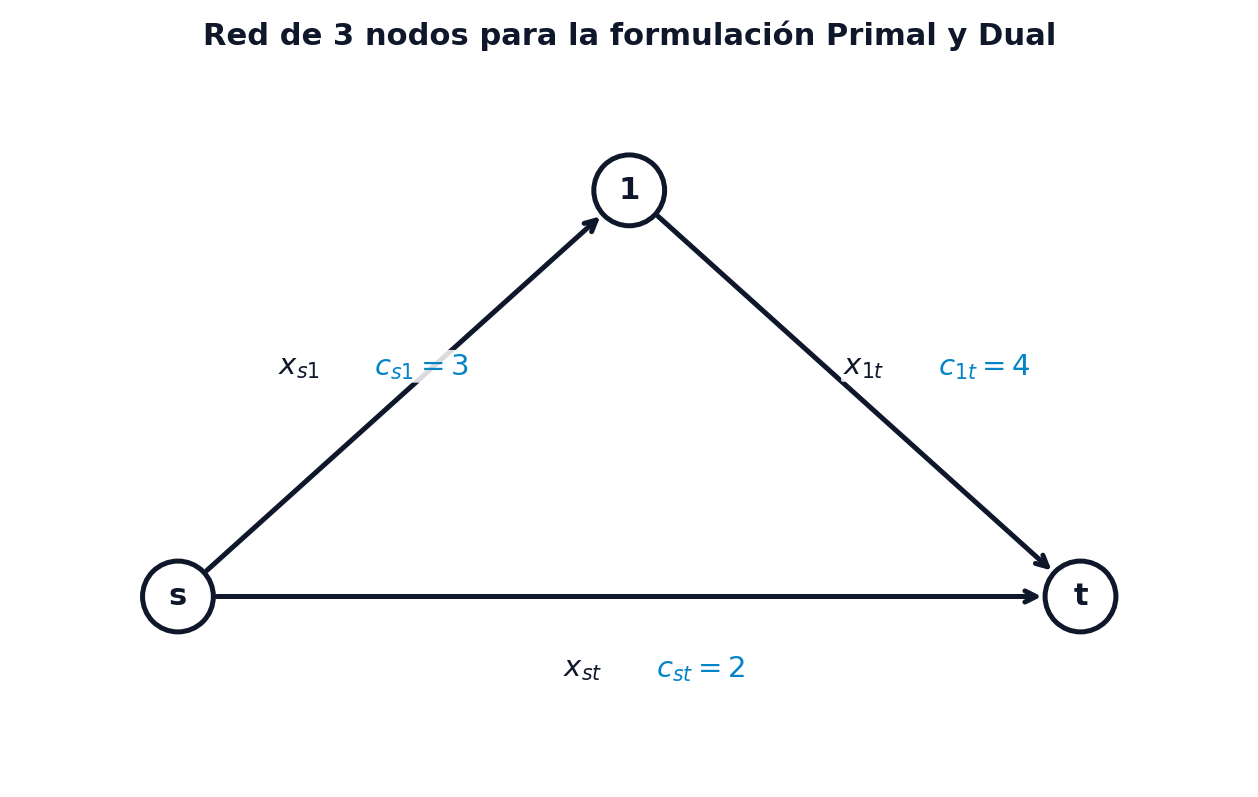
\includegraphics[width=0.6\linewidth,height=\textheight,keepaspectratio]{images/red_flujo_maximo_dualidad_ejemplo.png}

}

\caption{\label{fig-red-flujo-maximo-dualidad-ejemplo}Red de transporte
de 3 nodos para el planteamiento del problema de flujo máximo}

\end{figure}%

Planteando explícitamente el sistema de conservación de flujo para cada
vértice, el modelo primal resulta:

\[
\begin{aligned}
\max_{x, f_0} \quad & f_0 \\
\text{sujeto a} \quad & -x_{s1} - x_{st} = -f_0 \quad &(i = s) \\
& x_{s1} - x_{1t} = 0 \quad &(i = 1) \\
& x_{st} + x_{1t} = f_0 \quad &(i = t) \\
& x_{s1} \le 3, \quad x_{st} \le 2, \quad x_{1t} \le 4 \\
& x_{s1}, x_{st}, x_{1t} \ge 0
\end{aligned}
\]

Al eliminar la ecuación del sumidero \(t\) y fijar
\(u_t = 0 \implies u_s = 1\), las restricciones duales asociadas a cada
arco \(u_j - u_i + w_{ij} \ge 0\) se transforman en:

\[
\begin{aligned}
\min_{u, w} \quad & 3 w_{s1} + 2 w_{st} + 4 w_{1t} \\
\text{sujeto a} \quad & u_1 - u_s + w_{s1} \ge 0 \implies u_1 + w_{s1} \ge 1 \quad &(\text{arco } (s,1)) \\
& u_t - u_s + w_{st} \ge 0 \implies w_{st} \ge 1 \quad &(\text{arco } (s,t)) \\
& u_t - u_1 + w_{1t} \ge 0 \implies -u_1 + w_{1t} \ge 0 \quad &(\text{arco } (1,t)) \\
& w_{s1}, w_{st}, w_{1t} \ge 0
\end{aligned}
\]

La resolución de ambos modelos proporciona la solución primal óptima de
flujo máximo \(f_0^* = 5\) con \(x_{s1}^* = 3\), \(x_{st}^* = 2\) y
\(x_{1t}^* = 3\). Por su parte, la solución dual óptima asigna los
potenciales \(u_s = 1, u_1 = 0, u_t = 0\) y los multiplicadores de
capacidad \(w_{s1} = 1, w_{st} = 1, w_{1t} = 0\). El valor objetivo dual
es \(3(1) + 2(1) + 4(0) = 5 = f_0^*\), identificando de forma unívoca el
corte de capacidad mínima \(N = \{s\}\) con arcos salientes
\(w^+(N) = \{(s,1), (s,t)\}\) de capacidad \(3 + 2 = 5\), tal y como se
representa visualmente en la
Figura~\ref{fig-red-flujo-maximo-dualidad-solucion}:

\begin{figure}[H]

\centering{

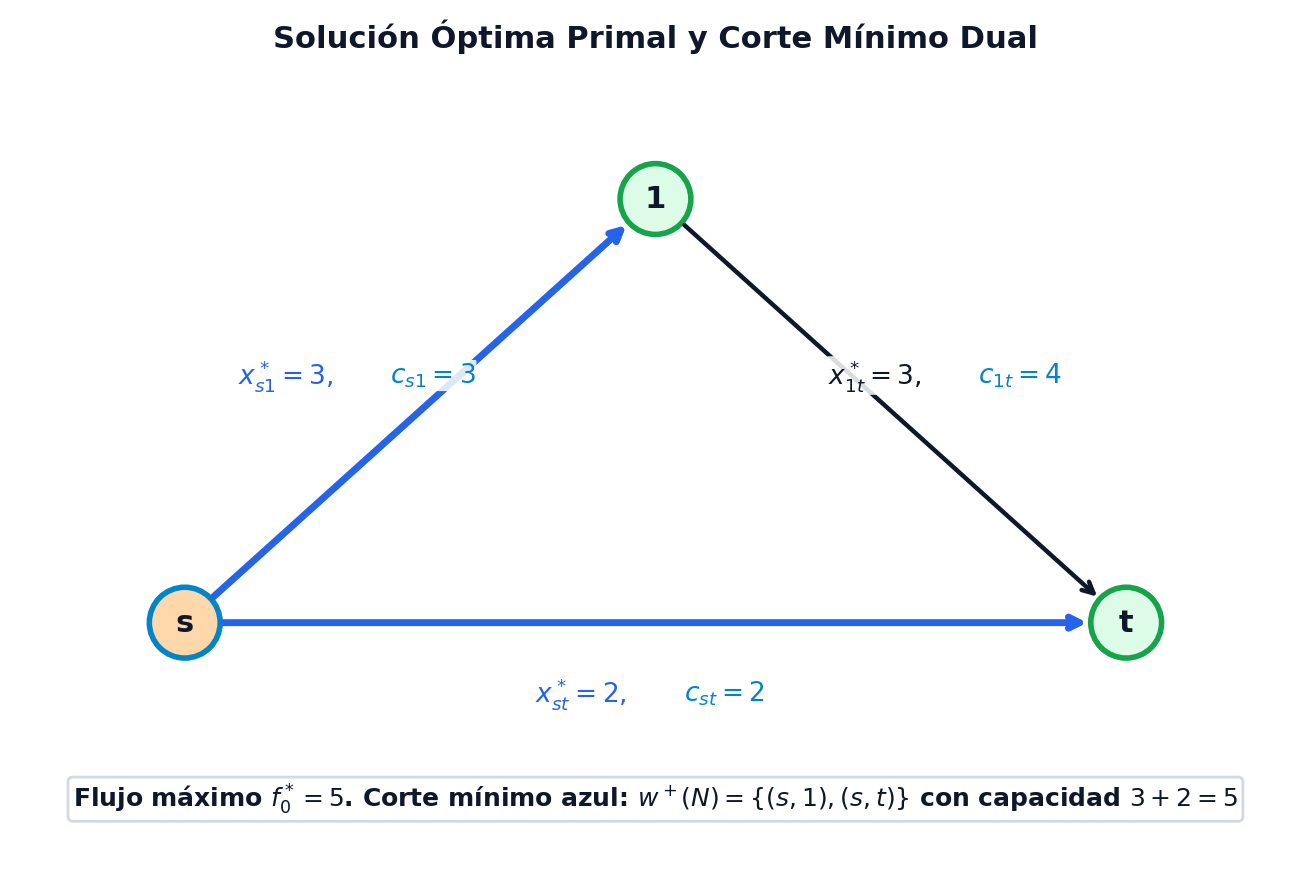
\includegraphics[width=0.6\linewidth,height=\textheight,keepaspectratio]{images/red_flujo_maximo_dualidad_solucion.png}

}

\caption{\label{fig-red-flujo-maximo-dualidad-solucion}Solución óptima
primal de flujo máximo y caracterización del corte de capacidad mínima
en el dual}

\end{figure}%

\end{tcolorbox}

\section{Problema de flujo a coste
mínimo}\label{problema-de-flujo-a-coste-muxednimo}

En los problemas de flujo máximo estudiados previamente, el único
objetivo estratégico consistía en determinar la máxima cantidad de
volumen que podía enviarse desde la fuente \(s\) al sumidero \(t\)
aprovechando las capacidades acotadas de los arcos. Sin embargo, en la
práctica logística, económica y de transporte (distribución de bienes,
encaminamiento de tráfico en redes de comunicación o asignación de
tareas), enviar flujo a través de diferentes caminos conlleva un
\textbf{coste unitario de transporte} \(p_{ij} \in \mathbb{R}\) por cada
unidad circulante.

\subsection{Planteamiento y formulación del flujo compatible a coste
mínimo}\label{planteamiento-y-formulaciuxf3n-del-flujo-compatible-a-coste-muxednimo}

Para comprender la necesidad de esta formulación, considérese el
\textbf{problema de asignación de tareas a máquinas}. Supóngase que se
dispone de un conjunto de \(n\) máquinas \(m_1, \dots, m_n\) y un
conjunto de \(n\) tareas \(t_1, \dots, t_n\). Tal y como se ilustra en
la Figura~\ref{fig-red-problema-asignacion-bipartita}, construyendo una
red de transporte bipartita donde la fuente \(s\) se conecta con
capacidad 1 a cada máquina, las máquinas con capacidad 1 a las tareas
que pueden ejecutar, y las tareas con capacidad 1 al sumidero \(t\), la
resolución del problema del flujo máximo determina el número máximo de
tareas realizables simultáneamente.

\begin{figure}

\centering{

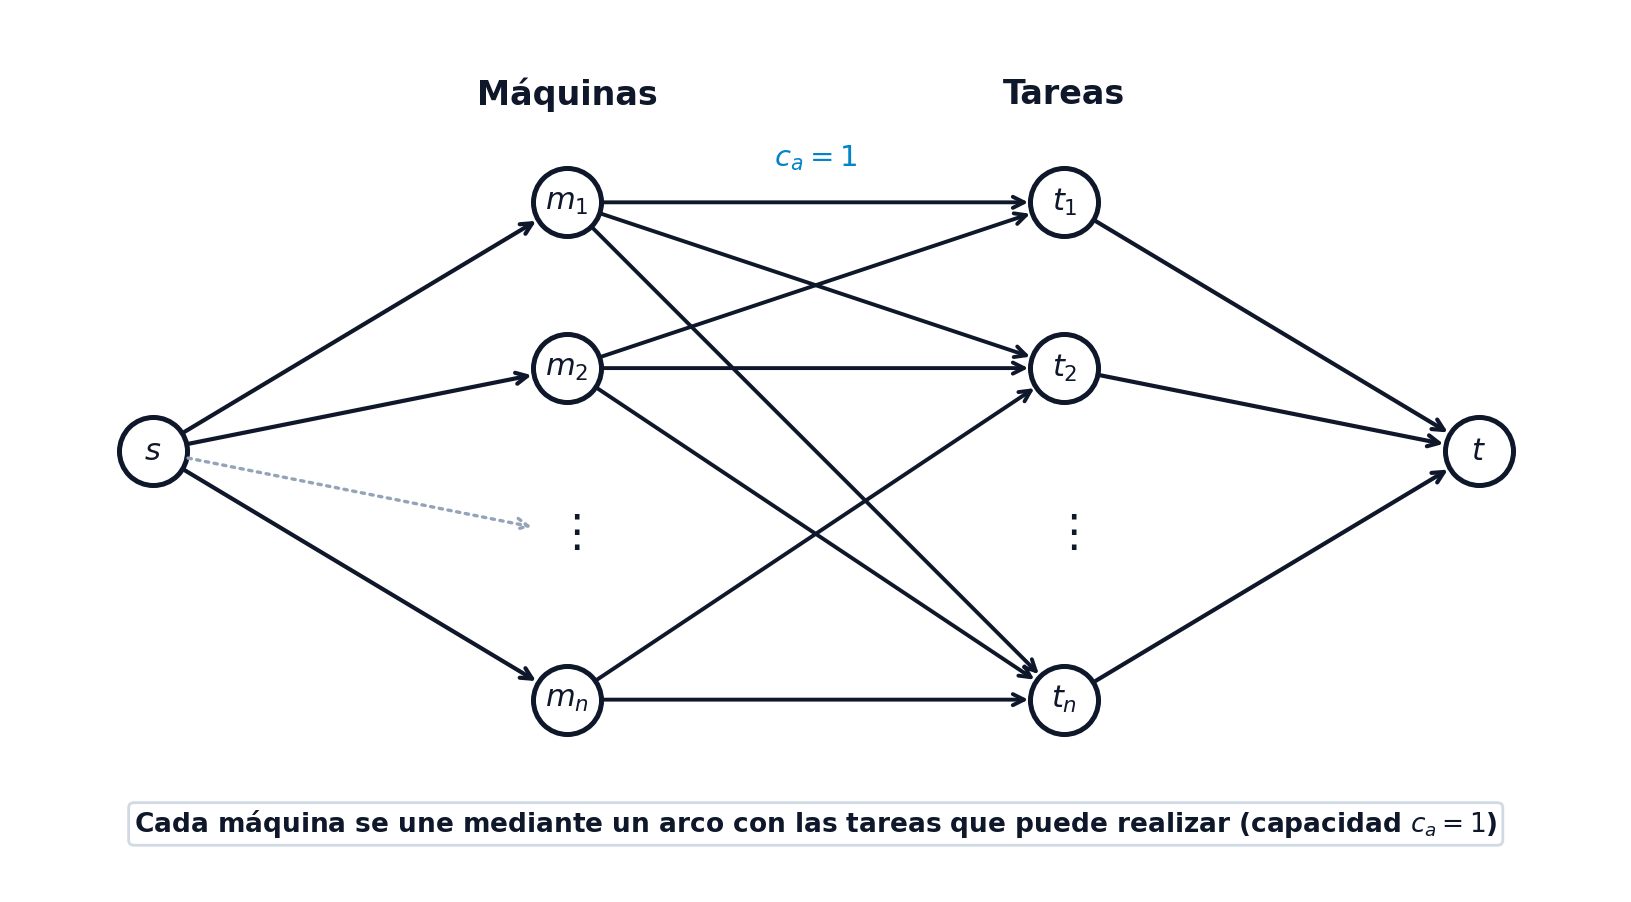
\includegraphics[width=0.75\linewidth,height=\textheight,keepaspectratio]{images/red_problema_asignacion_bipartita.png}

}

\caption{\label{fig-red-problema-asignacion-bipartita}Representación en
red de flujo del problema de asignación de tareas a máquinas}

\end{figure}%

No obstante, en la realidad industrial cada máquina \(m_i\) incurre en
un coste de procesamiento o ejecución distinto \(p_{ij}\) al realizar la
tarea \(t_j\). El objetivo óptimo ya no es únicamente ejecutar el máximo
número de tareas, sino hallar la asignación completa que minimice el
coste total invertido.

Generalizando este escenario, dada una red de transporte
\((G = (V, U), \mathbf{c})\) equipada con capacidades \(c_{ij} \ge 0\),
costes unitarios \(p_{ij} \in \mathbb{R}\) y un valor prefijado de flujo
a enviar \(f_0 = \nu\) entre la fuente \(s\) y el sumidero \(t\), el
\textbf{problema del flujo compatible a coste mínimo} se formula
analíticamente como el siguiente programa lineal:

\[
\begin{aligned}
\min_{f} \quad & \sum_{(i,j) \in U} p_{ij} f_{ij} \\
\text{sujeto a} \quad & \sum_{j \mid (j, i) \in U} f_{ji} - \sum_{j \mid (i, j) \in U} f_{ij} = \begin{cases} -\nu & \text{si } i = s \\ 0 & \text{si } i \neq s, t \\ \nu & \text{si } i = t \end{cases} \quad \forall i \in V \\
& 0 \le f_{ij} \le c_{ij}, \quad \forall (i, j) \in U
\end{aligned}
\]

\begin{tcolorbox}[enhanced jigsaw, toprule=.15mm, opacitybacktitle=0.6, coltitle=black, colbacktitle=quarto-callout-tip-color!10!white, title=\textcolor{quarto-callout-tip-color}{\faLightbulb}\hspace{0.5em}{Ejemplo: Comparación de flujos compatibles y circulación por ciclos}, arc=.35mm, rightrule=.15mm, toptitle=1mm, breakable, bottomtitle=1mm, titlerule=0mm, colback=white, opacityback=0, leftrule=.75mm, colframe=quarto-callout-tip-color-frame, left=2mm, bottomrule=.15mm]

Considérese la red de transporte de 5 nodos \(V = \{s, a, b, c, t\}\)
representada en la Figura~\ref{fig-red-flujo-coste-minimo-ejemplo},
donde cada arco contiene el identificador de arista (1 a 6) y la
etiqueta \((c_{ij})[p_{ij}]\) especificando su capacidad \(c_{ij}\) en
azul entre paréntesis y su coste unitario \(p_{ij}\) en rojo entre
corchetes:

\begin{figure}[H]

\centering{

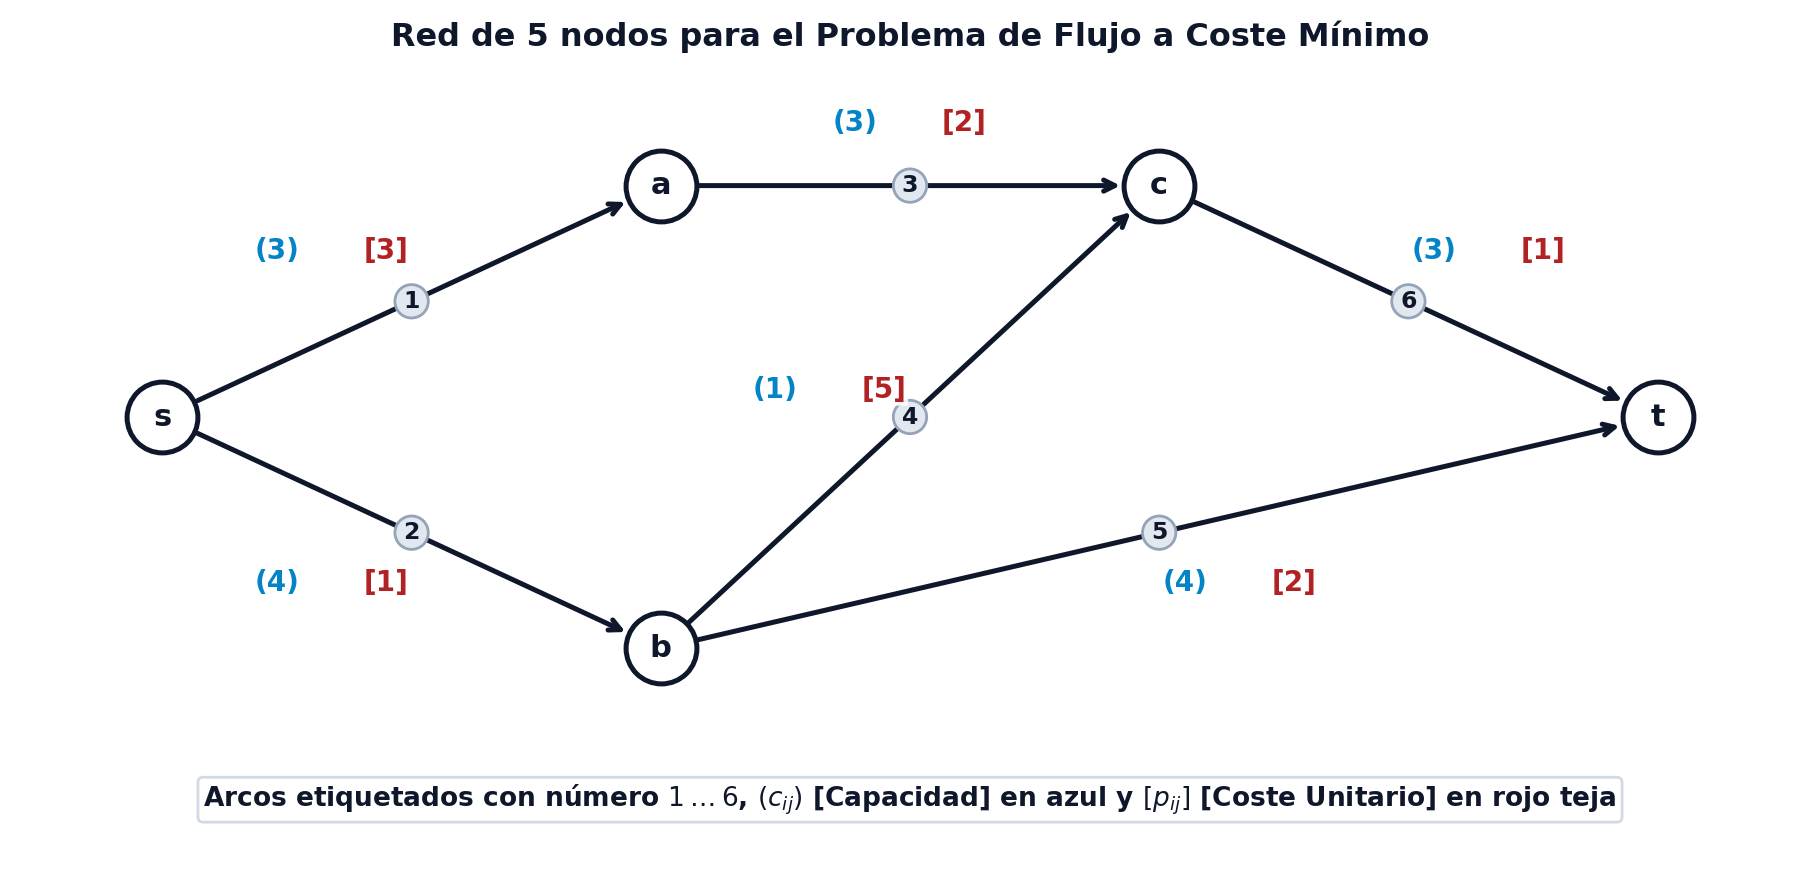
\includegraphics[width=0.7\linewidth,height=\textheight,keepaspectratio]{images/red_flujo_coste_minimo_ejemplo.png}

}

\caption{\label{fig-red-flujo-coste-minimo-ejemplo}Red de transporte de
5 nodos para el problema de flujo a coste mínimo}

\end{figure}%

Supóngase que se desea enviar un flujo total prefijado de \(\nu = 4\)
unidades desde la fuente \(s\) al sumidero \(t\). Como se ilustra en la
Figura~\ref{fig-comparacion-flujos-coste-minimo}, existen múltiples
asignaciones compatibles de flujo. Analicemos dos soluciones factibles
particulares, \(\mathbf{f}^A\) (destacada en rojo) y \(\mathbf{f}^B\)
(destacada en azul), cuyos costes totales \(c_A = 19\) y \(c_B = 18\) se
desglosan en la recuadros superiores derechos de la figura:

\begin{figure}[H]

\centering{

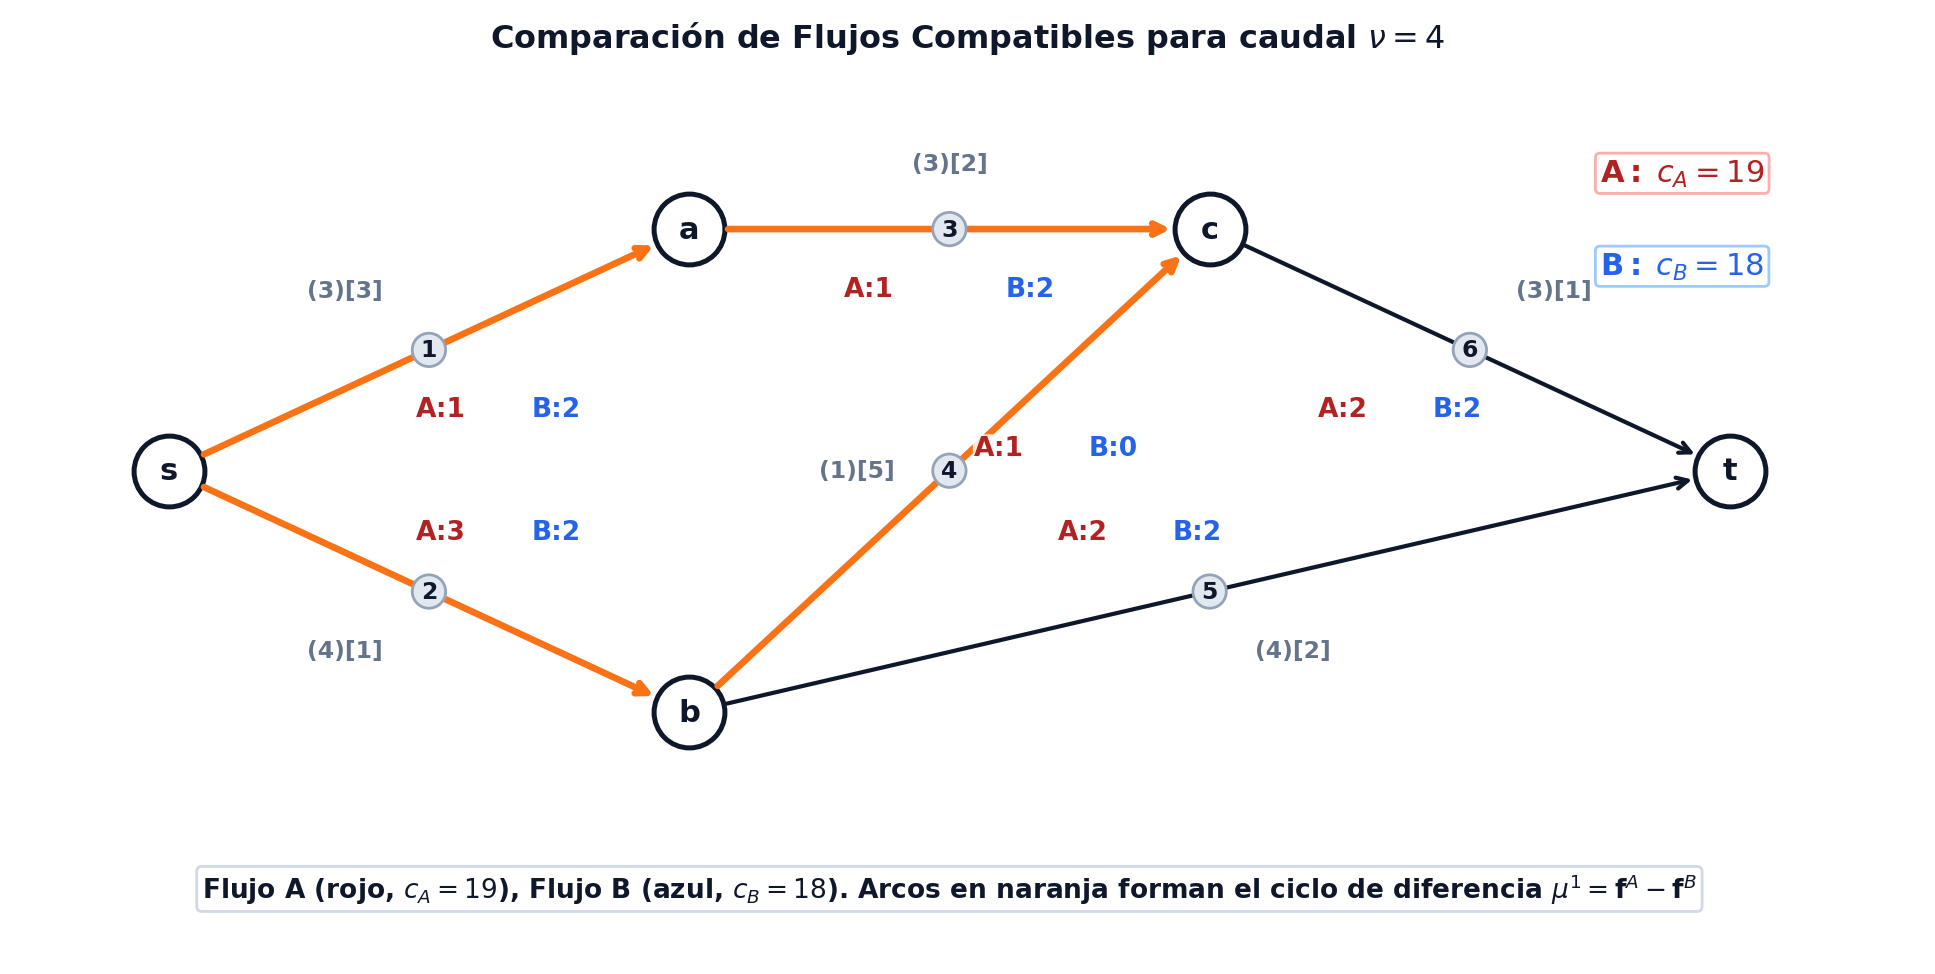
\includegraphics[width=0.75\linewidth,height=\textheight,keepaspectratio]{images/comparacion_flujos_coste_minimo.png}

}

\caption{\label{fig-comparacion-flujos-coste-minimo}Comparación de dos
flujos compatibles A y B de valor caudal 4 con sus costes totales y
caracterización del ciclo de diferencia}

\end{figure}%

\begin{enumerate}
\def\labelenumi{\arabic{enumi}.}
\tightlist
\item
  \textbf{Flujo Compatible \(\mathbf{f}^A\)} (en rojo):

  \begin{itemize}
  \tightlist
  \item
    Asignación:
    \(f_{sa}^A=1, f_{sb}^A=3, f_{ac}^A=1, f_{bc}^A=1, f_{bt}^A=2, f_{ct}^A=2\).
  \item
    Coste Total:
    \(c_A = 1(3) + 3(1) + 1(2) + 1(5) + 2(2) + 2(1) = 3 + 3 + 2 + 5 + 4 + 2 = 19\).
  \end{itemize}
\item
  \textbf{Flujo Compatible \(\mathbf{f}^B\)} (en azul):

  \begin{itemize}
  \tightlist
  \item
    Asignación:
    \(f_{sa}^B=2, f_{sb}^B=2, f_{ac}^B=2, f_{bc}^B=0, f_{bt}^B=2, f_{ct}^B=2\).
  \item
    Coste Total:
    \(c_B = 2(3) + 2(1) + 2(2) + 0(5) + 2(2) + 2(1) = 6 + 2 + 4 + 0 + 4 + 2 = 18\).
  \end{itemize}
\end{enumerate}

\textbf{Análisis de la Diferencia entre Soluciones (Circulación
Cíclica)}:

Calculando la diferencia vectorial componente a componente
\(\mathbf{\mu}^1 = \mathbf{f}^A - \mathbf{f}^B\), se obtiene la tupla de
variaciones \(\mathbf{\mu}^1 = (-1, 1, -1, 1, 0, 0)\). Gráficamente,
estos cuatro arcos modificados forman un \textbf{circuito cerrado}
\(s \to b \to c \to a \to s\).

Por lo tanto, es posible pasar del flujo no óptimo \(\mathbf{f}^A\) al
flujo de menor coste \(\mathbf{f}^B\) simplemente \textbf{sumando un
ciclo incremental orientado en sentido inverso \(-\mathbf{\mu}^1\)}. La
diferencia de coste total entre ambas soluciones es exactamente el coste
neto de recorrer dicho ciclo: \(c_A - c_B = 19 - 18 = 1\). Este
resultado demuestra de manera intuitiva que \textbf{la diferencia entre
dos flujos cualesquiera de igual valor \(\nu\) es siempre una
combinación lineal de circuitos residuales}.

\textbf{Análisis Inicial de Cadenas desde el Flujo Nulo
(\(\nu_0 = 0\))}:

Para construir directamente la solución de coste mínimo sin tanteos
arbitrarios, observamos que para un caudal inicial \(\nu_0 = 0\) el
flujo nulo \(\mathbf{f}^0 = \mathbf{0}\) es trivialmente óptimo (coste
0). En la red inicial existen tres cadenas orientadas simples desde la
fuente \(s\) al sumidero \(t\):

\begin{itemize}
\tightlist
\item
  \textbf{Cadena 1} (\(s \to a \to c \to t\)): Coste total residual
  \(p(\mu_1) = 3 + 2 + 1 = 6\).
\item
  \textbf{Cadena 2} (\(s \to b \to t\)): Coste total residual
  \(p(\mu_2) = 1 + 2 = 3\).
\item
  \textbf{Cadena 3} (\(s \to b \to c \to t\)): Coste total residual
  \(p(\mu_3) = 1 + 5 + 1 = 7\).
\end{itemize}

La cadena de coste mínimo es \(s \to b \to t\) con coste unitario 3 y
capacidad residual \(\min(4, 4) = 4\). Por tanto, para enviar un caudal
\(\nu = 4\), la solución óptima absoluta consiste en canalizar las 4
unidades íntegramente por \(s \to b \to t\), alcanzando un coste óptimo
mínimo de \(4 \times 3 = 12\) (estrictamente menor que los costes 19 y
18 de las soluciones de prueba \(\mathbf{f}^A\) y \(\mathbf{f}^B\)).

\end{tcolorbox}

\subsection{Teoremas de optimalidad y caracterización de
circuitos}\label{teoremas-de-optimalidad-y-caracterizaciuxf3n-de-circuitos}

Para formalizar algebraicamente el criterio de parada y las condiciones
necesarias y suficientes de coste mínimo, se introducen las siguientes
definiciones sobre cadenas e incrementos en redes con costes.

\begin{tcolorbox}[enhanced jigsaw, toprule=.15mm, opacitybacktitle=0.6, coltitle=black, colbacktitle=quarto-callout-note-color!10!white, title=\textcolor{quarto-callout-note-color}{\faInfo}\hspace{0.5em}{Definición: Coste de una cadena y cadenas incrementales}, arc=.35mm, rightrule=.15mm, toptitle=1mm, breakable, bottomtitle=1mm, titlerule=0mm, colback=white, opacityback=0, leftrule=.75mm, colframe=quarto-callout-note-color-frame, left=2mm, bottomrule=.15mm]

\begin{enumerate}
\def\labelenumi{\arabic{enumi}.}
\item
  \textbf{Coste de una Cadena}: Dada una cadena orientada \(\mu\)
  formada por arcos directos \(\mu^+\) e inversos \(\mu^-\), el coste
  total residual de la cadena se define sumando los costes unitarios
  según la orientación de paso: \[
  p(\mu) = \sum_{u \in \mu^+} p_u - \sum_{u \in \mu^-} p_u
  \]
\item
  \textbf{Cadena Incremental}: Una cadena \(\mu\) es incremental
  respecto a un flujo \(\mathbf{f}\) si admite un incremento positivo de
  flujo \(\delta > 0\) sin violar la no negatividad ni superar la
  capacidad física de ningún arco (\(f_u < c_u, \forall u \in \mu^+\) y
  \(f_u > 0, \forall u \in \mu^-\)).
\end{enumerate}

\end{tcolorbox}

A partir de estas nociones se establecen los dos teoremas fundamentales
que rigen la optimización de flujos con coste.

\begin{tcolorbox}[enhanced jigsaw, toprule=.15mm, opacitybacktitle=0.6, coltitle=black, colbacktitle=quarto-callout-important-color!10!white, title=\textcolor{quarto-callout-important-color}{\faExclamation}\hspace{0.5em}{Teorema 1: Optimalidad por ausencia de circuitos incrementales de coste
negativo}, arc=.35mm, rightrule=.15mm, toptitle=1mm, breakable, bottomtitle=1mm, titlerule=0mm, colback=white, opacityback=0, leftrule=.75mm, colframe=quarto-callout-important-color-frame, left=2mm, bottomrule=.15mm]

Un flujo compatible \(\mathbf{f}\) de valor \(f_0 = \nu\) es de
\textbf{coste mínimo} si y solo si la red residual \(G(\mathbf{f})\)
\textbf{no contiene ningún circuito incremental de coste total negativo}
(sin incluir el arco ficticio de retorno \((t, s)\)).

\emph{Demostración}: Cualquier otro flujo factible \(\mathbf{f}'\) de
valor \(\nu\) puede expresarse algebraicamente como la suma del flujo
\(\mathbf{f}\) y una combinación lineal de circulaciones cíclicas
simples \(\mathbf{f}' - \mathbf{f} = \sum \alpha_k \mathbf{\mu}^k\). Si
existiera en la red residual un circuito incremental \(\mathbf{\mu}^k\)
con coste estrictamente negativo (\(p(\mu^k) < 0\)), aumentar el flujo a
lo largo de \(\mathbf{\mu}^k\) mantendría inalterado el caudal \(\nu\)
(ya que las circulaciones de ciclo no tienen fuente ni sumidero) pero
reduciría estrictamente el coste total, lo que contradice la minimidad
de \(\mathbf{f}'\). Recíprocamente, si no existen circuitos
incrementales de coste negativo, ninguna modificación cíclica puede
reducir el coste, garantizando la optimalidad global. \(\blacksquare\)

\end{tcolorbox}

La verificación de la optimalidad mediante el \textbf{Teorema 1}
constituye la base teórica para validar si un flujo determinado es el
más económico posible para un caudal fijo \(\nu\). Dado que cualquier
flujo factible puede visualizarse como el flujo actual corregido por una
serie de circulaciones cíclicas, la ausencia de ciclos de mejora
(aquellos que reducen el coste) garantiza que nos encontramos en un
óptimo local y global. Para extender este resultado a un procedimiento
de construcción progresiva, necesitamos el siguiente teorema de
crecimiento incremental.

\begin{tcolorbox}[enhanced jigsaw, toprule=.15mm, opacitybacktitle=0.6, coltitle=black, colbacktitle=quarto-callout-important-color!10!white, title=\textcolor{quarto-callout-important-color}{\faExclamation}\hspace{0.5em}{Teorema 2: Incrementos por caminos de coste mínimo}, arc=.35mm, rightrule=.15mm, toptitle=1mm, breakable, bottomtitle=1mm, titlerule=0mm, colback=white, opacityback=0, leftrule=.75mm, colframe=quarto-callout-important-color-frame, left=2mm, bottomrule=.15mm]

Dado un flujo \(\mathbf{f}\) de valor \(\nu\) que es de coste mínimo, si
se incrementa el flujo en \(\delta\) unidades a lo largo de la cadena
incremental de \(s\) a \(t\) que posea el \textbf{coste total residual
mínimo} en \(G(\mathbf{f})\), el flujo resultante es de coste mínimo
para el nuevo caudal \(\nu + \delta\).

\emph{Demostración}: Partiendo de la solución a coste mínimo para un
valor de flujo \(\nu\), se encuentra una cadena incremental de \(s\) a
\(t\) de coste mínimo \(p(\mu)\). Se debe demostrar que al incrementar
el flujo en \(\delta\) unidades a lo largo de dicha cadena, la solución
resultante es de coste mínimo para el nuevo valor \(\nu + \delta\).

Por reducción al absurdo y aplicando el \textbf{Teorema 1}, supóngase
que la nueva solución no fuera óptima para \(\nu + \delta\). En tal
caso, debería existir en la red residual un ciclo incremental de coste
estrictamente negativo:

\begin{enumerate}
\def\labelenumi{\arabic{enumi}.}
\tightlist
\item
  \textbf{Si el ciclo NO comparte arcos con la cadena}: El ciclo ya
  pertenecía a la red residual de la solución inicial, lo que implicaría
  que la solución inicial no habría sido de coste mínimo para \(\nu\),
  contradiciendo la hipótesis.
\item
  \textbf{Si el ciclo y la cadena comparten arcos}: Uniendo
  vectorialmente ambos se puede construir una nueva cadena incremental
  de \(s\) a \(t\) con un coste estrictamente menor que \(p(\mu)\), lo
  cual contradice que la cadena original fuera de coste mínimo.
\end{enumerate}

Al ser ambos casos imposibles, se concluye que el flujo incrementado en
\(\delta\) unidades es de coste mínimo para \(\nu + \delta\).
\(\blacksquare\)

\end{tcolorbox}

El \textbf{Teorema 2} valida la estrategia de construcción iterativa: no
necesitamos realizar un cálculo de optimización global completo para
cada valor de flujo, sino que basta con encadenar aumentos de caudal a
lo largo de los caminos más eficientes disponibles en la red residual.
Esta propiedad garantiza que cada paso algorítmico preserva la
optimalidad, permitiendo avanzar de forma eficiente desde \(f_0=0\)
hasta la meta \(\nu\).

\begin{tcolorbox}[enhanced jigsaw, toprule=.15mm, opacitybacktitle=0.6, coltitle=black, colbacktitle=quarto-callout-note-color!10!white, title=\textcolor{quarto-callout-note-color}{\faInfo}\hspace{0.5em}{Nota: Estrategia algorítmica de resolución iterativa}, arc=.35mm, rightrule=.15mm, toptitle=1mm, breakable, bottomtitle=1mm, titlerule=0mm, colback=white, opacityback=0, leftrule=.75mm, colframe=quarto-callout-note-color-frame, left=2mm, bottomrule=.15mm]

La combinación didáctica de ambos teoremas proporciona el esquema
general de resolución:

\begin{enumerate}
\def\labelenumi{\arabic{enumi}.}
\item
  \textbf{Determinación de la Solución Inicial (Teorema 1)}: Se puede
  iniciar el proceso desde el flujo nulo \(\mathbf{f}^0 = \mathbf{0}\)
  para \(\nu = 0\). Si todos los costes unitarios son no negativos
  (\(p_{ij} \ge 0\)), no existe ningún circuito inicial de coste
  negativo y \(\mathbf{f}^0\) es trivialmente óptimo. Si existen costes
  negativos, se aplican algoritmos de detección de ciclos negativos
  (como Bellman-Ford) para eliminar circulaciones iniciales negativas
  aplicando el Teorema 1.
\item
  \textbf{Crecimiento Iterativo por Caminos Mínimos (Teorema 2)}: A
  partir del flujo óptimo inicial, se calcula iterativamente la cadena
  de coste residual mínimo desde \(s\) hasta \(t\) y se incrementa el
  flujo en \(\delta\) unidades. Por el Teorema 2, cada paso garantiza la
  optimalidad del nuevo caudal \(\nu + \delta\), repitiendo la búsqueda
  hasta alcanzar el volumen objetivo \(\nu\) prefijado en el problema.
\end{enumerate}

\end{tcolorbox}

\subsection{Algoritmo de Flujo a Coste Mínimo (Grafo de
distancias)}\label{algoritmo-de-flujo-a-coste-muxednimo-grafo-de-distancias}

El problema de hallar cadenas incrementales de coste mínimo en la red
inicial se traduce operacionalmente en encontrar \textbf{caminos de
longitud mínima} entre la fuente \(s\) y el sumidero \(t\) en el grafo
de distancias residual \(G(\mathbf{f})\). Una vez obtenido el camino más
corto, el siguiente paso consiste en determinar el incremento máximo de
flujo compatible a lo largo de sus arcos. La detección temprana de
circuitos negativos en este grafo permite asegurar que el estado inicial
del sistema es coherente con los principios de optimalidad descritos
anteriormente.

\begin{tcolorbox}[enhanced jigsaw, toprule=.15mm, opacitybacktitle=0.6, coltitle=black, colbacktitle=quarto-callout-note-color!10!white, title=\textcolor{quarto-callout-note-color}{\faInfo}\hspace{0.5em}{Nota: Correspondencia de circuitos negativos}, arc=.35mm, rightrule=.15mm, toptitle=1mm, breakable, bottomtitle=1mm, titlerule=0mm, colback=white, opacityback=0, leftrule=.75mm, colframe=quarto-callout-note-color-frame, left=2mm, bottomrule=.15mm]

Cualquier circuito de longitud total estrictamente negativa en el grafo
residual \(G(\mathbf{f})\) se corresponde de forma unívoca con un
\textbf{ciclo incremental de coste negativo} en la red de transporte
original.

\end{tcolorbox}

\begin{tcolorbox}[enhanced jigsaw, toprule=.15mm, opacitybacktitle=0.6, coltitle=black, colbacktitle=quarto-callout-note-color!10!white, title=\textcolor{quarto-callout-note-color}{\faInfo}\hspace{0.5em}{Esquema: Algoritmo de Flujo a Coste Mínimo}, arc=.35mm, rightrule=.15mm, toptitle=1mm, breakable, bottomtitle=1mm, titlerule=0mm, colback=white, opacityback=0, leftrule=.75mm, colframe=quarto-callout-note-color-frame, left=2mm, bottomrule=.15mm]

\begin{itemize}
\item
  \textbf{Paso 1: Inicialización}: Obtener un flujo compatible inicial
  \(\mathbf{f}\) (habitualmente el flujo nulo
  \(\mathbf{f}^0 = \mathbf{0}\) para \(\nu = 0\)).
\item
  \textbf{Paso 2: Eliminación de ciclos con coste negativo}:

  \begin{enumerate}
  \def\labelenumi{\arabic{enumi}.}
  \tightlist
  \item
    Construir el grafo de distancias residual \(G(\mathbf{f})\).
  \item
    Si \(G(\mathbf{f})\) contiene circuitos de longitud negativa,
    modificar el flujo incrementándolo a lo largo del circuito en su
    capacidad residual y volver al Paso 2.1.
  \item
    En caso contrario (sin circuitos negativos), ir al \textbf{Paso 3}.
  \end{enumerate}
\item
  \textbf{Paso 3: Aumento del valor del flujo}:

  \begin{itemize}
  \tightlist
  \item
    Si el valor del flujo ha alcanzado la meta \(f_0 = \nu\),
    \textbf{PARAR}: Solución óptima alcanzada.
  \item
    En caso contrario (\(f_0 < \nu\)), buscar en \(G(\mathbf{f})\) el
    camino de longitud mínima de \(s\) a \(t\):

    \begin{enumerate}
    \def\labelenumi{\arabic{enumi}.}
    \tightlist
    \item
      Si no existe ningún camino de \(s\) a \(t\) en \(G(\mathbf{f})\),
      \textbf{PARAR}: El problema no admite solución factible para el
      valor de flujo \(\nu\).
    \item
      En caso contrario, calcular la capacidad residual mínima de la
      cadena asociada al camino \(c(s, t)\).
    \item
      Variar el flujo en los arcos del camino en la cantidad
      \(\Delta = \min\{c(s, t), \nu - f_0\}\).
    \item
      Actualizar el flujo \(f_0 \leftarrow f_0 + \Delta\), construir el
      grafo residual asociado al nuevo flujo e ir al \textbf{Paso 3}.
    \end{enumerate}
  \end{itemize}
\end{itemize}

\end{tcolorbox}

\begin{tcolorbox}[enhanced jigsaw, toprule=.15mm, opacitybacktitle=0.6, coltitle=black, colbacktitle=quarto-callout-tip-color!10!white, title=\textcolor{quarto-callout-tip-color}{\faLightbulb}\hspace{0.5em}{Ejemplo: Traza del algoritmo de flujo a coste mínimo}, arc=.35mm, rightrule=.15mm, toptitle=1mm, breakable, bottomtitle=1mm, titlerule=0mm, colback=white, opacityback=0, leftrule=.75mm, colframe=quarto-callout-tip-color-frame, left=2mm, bottomrule=.15mm]

Considérese la red de transporte de 5 nodos \(V = \{s, a, b, c, t\}\)
con 7 arcos dirigidos \(U = \{1, 2, 3, 4, 5, 6, 7\}\), cuyas capacidades
\(c_{ij}\) y costes unitarios \(p_{ij}\) se expresan en el formato
\((c_{ij})[p_{ij}]\):

\begin{itemize}
\tightlist
\item
  Arco 1: \((s, a)\) con capacidad \(c_{sa} = 3\) y coste
  \(p_{sa} = 3\).
\item
  Arco 2: \((s, b)\) con capacidad \(c_{sb} = 2\) y coste
  \(p_{sb} = 3\).
\item
  Arco 3: \((a, c)\) con capacidad \(c_{ac} = 2\) y coste
  \(p_{ac} = -1\).
\item
  Arco 4: \((a, t)\) con capacidad \(c_{at} = 4\) y coste
  \(p_{at} = -1\).
\item
  Arco 5: \((b, a)\) con capacidad \(c_{ba} = 2\) y coste
  \(p_{ba} = -2\).
\item
  Arco 6: \((c, b)\) con capacidad \(c_{cb} = 2\) y coste
  \(p_{cb} = 1\).
\item
  Arco 7: \((c, t)\) con capacidad \(c_{ct} = 5\) y coste
  \(p_{ct} = 2\).
\end{itemize}

Se desea transmitir un caudal total objetivo de \(\nu = 5\) unidades
desde la fuente \(s\) al sumidero \(t\) al menor coste total posible.

\textbf{Paso a paso de los cálculos e iteraciones}

\textbf{Paso 1: Inicialización}

Se inicia el procedimiento fijando la solución de flujo nulo
\(\mathbf{f}^0 = \mathbf{0}\) para un valor de caudal circulante de
\(f_0 = 0\). El coste acumulado inicial es
\(C(\mathbf{f}^0) = \sum_{(i,j) \in U} p_{ij} f_{ij}^0 = 0\).

\textbf{Paso 2: Eliminación de circuitos con coste negativo}

\begin{itemize}
\item
  \textbf{Paso 2.1: Construcción de \(G(\mathbf{f}^0)\)}: Puesto que el
  flujo es nulo en todos los arcos (\(f_{ij}^0 = 0\)), todos los arcos
  directos admiten capacidad residual
  \(c_{ij} - f_{ij}^0 = c_{ij} > 0\). Se construye \(G(\mathbf{f}^0)\)
  asignando a cada arco su peso unitario \(p_{ij}\):
  \[p_{sa} = 3, \quad p_{sb} = 3, \quad p_{ba} = -2, \quad p_{ac} = -1, \quad p_{cb} = 1, \quad p_{at} = -1, \quad p_{ct} = 2\]
\item
  \textbf{Paso 2.2: Detección del circuito residual de longitud
  negativa}: Evaluando los circuitos cerrados en \(G(\mathbf{f}^0)\), se
  identifica el circuito orientado \(C_1 = a \to c \to b \to a\).
  Calculamos su coste total:
  \[p(C_1) = p_{ac} + p_{cb} + p_{ba} = (-1) + 1 + (-2) = -2 < 0\]

  Al ser \(p(C_1) = -2 < 0\), por el \textbf{Teorema 1} el flujo nulo
  \(\mathbf{f}^0\) no es óptimo porque es posible reducir el coste
  circulando flujo en ciclo. Determinamos la \textbf{Capacidad Residual
  Máxima} \(\delta_1\) de \(C_1\):
  \[\delta_1 = \min \{ c_{ac} - f_{ac}^0, \, c_{cb} - f_{cb}^0, \, c_{ba} - f_{ba}^0 \} = \min \{ 2 - 0, \, 2 - 0, \, 2 - 0 \} = 2 \text{ unidades}\]
\item
  \textbf{Paso 2.3: Incremento de flujo en el circuito y recálculo del
  coste}: Incrementamos el flujo en \(\delta_1 = 2\) unidades a lo largo
  de \(C_1\): \[f_{ac}^1 = 2, \quad f_{cb}^1 = 2, \quad f_{ba}^1 = 2\]

  El resto de arcos mantienen su flujo nulo. Recalculamos el coste total
  acumulado del nuevo flujo \(\mathbf{f}^1\):
  \[C(\mathbf{f}^1) = 2(p_{ac}) + 2(p_{cb}) + 2(p_{ba}) = 2(-1) + 2(1) + 2(-2) = -4\]

  El coste total disminuye de \(0\) a \(-4\) manteniendo el caudal
  entrante en la fuente igual a \(f_0 = 0\).
\item
  \textbf{Paso 2.4: Nuevo grafo residual \(G(\mathbf{f}^1)\) y
  verificación}: Al estar los arcos \((a, c)\), \((c, b)\) y \((b, a)\)
  saturados (\(f = c = 2\)), los arcos directos desaparecen de
  \(G(\mathbf{f}^1)\) y se activan sus arcos inversos:

  \begin{itemize}
  \tightlist
  \item
    Arco inverso \((c, a)\) con peso \(-p_{ac} = -(-1) = 1\).
  \item
    Arco inverso \((b, c)\) con peso \(-p_{cb} = -1\).
  \item
    Arco inverso \((a, b)\) con peso \(-p_{ba} = -(-2) = 2\).
  \end{itemize}

  Se comprueba en \(G(\mathbf{f}^1)\) que \textbf{ya no existe ningún
  circuito de longitud negativa}. Por el \textbf{Teorema 1}, el flujo
  \(\mathbf{f}^1\) es el punto de partida óptimo para caudal
  \(f_0 = 0\).
\end{itemize}

\textbf{Paso 3: Aumento del valor del flujo}

Como el caudal actual \(f_0 = 0\) es estrictamente menor que la meta
\(\nu = 5\), aplicamos iterativamente el Paso 3 buscando caminos de
longitud mínima entre \(s\) y \(t\) en el grafo residual:

\begin{itemize}
\tightlist
\item
  \textbf{Primera iteración del Paso 3 (Caudal \(f_0 = 0 \to 3\))}:

  \begin{enumerate}
  \def\labelenumi{\arabic{enumi}.}
  \tightlist
  \item
    \textbf{Paso 3.1 (Camino Mínimo en \(G(\mathbf{f}^1)\))}: Buscamos
    en \(G(\mathbf{f}^1)\) el camino de longitud residual mínima entre
    \(s\) y \(t\). Se encuentra el camino mínimo
    \(\mu_1 = s \to a \to t\) con coste residual
    \(p(\mu_1) = p_{sa} + p_{at} = 3 + (-1) = 2\).
  \item
    \textbf{Paso 3.2 (Capacidad residual e incremento)}: Capacidad
    residual de la cadena \(c(\mu_1) = \min \{ 3 - 0, \, 4 - 0 \} = 3\)
    unidades. Incremento de flujo:
    \(\Delta_1 = \min \{ 3, \, 5 - 0 \} = 3\) unidades.
  \item
    \textbf{Paso 3.3 (Actualización de flujos)}: Asignamos
    \(\Delta_1 = 3\) unidades a lo largo de \(\mu_1\):
    \(f_{sa}^2 = 3, f_{at}^2 = 3\). El caudal circulante alcanza
    \(f_0 = 3\). Coste acumulado: \(C(\mathbf{f}^2) = -4 + 3(2) = 2\).
  \item
    \textbf{Paso 3.4 (Nuevo Grafo Residual \(G(\mathbf{f}^2)\))}: El
    arco \((s, a)\) queda saturado (\(f_{sa} = 3 = c_{sa}\)), generando
    el arco inverso \((a, s)\) con peso \(-3\). El arco \((a, t)\) está
    parcialmente cargado (\(f_{at} = 3 < 4\)), manteniendo el arco
    directo \((a, t)\) con peso \(-1\) en el grafo azul (y \(+1\) al
    recorrerlo en la figura del camino) y el arco inverso \((t, a)\) con
    peso \(+1\).
  \end{enumerate}
\item
  \textbf{Segunda iteración del Paso 3 (Caudal \(f_0 = 3 \to 4\))}:

  \begin{enumerate}
  \def\labelenumi{\arabic{enumi}.}
  \item
    \textbf{Paso 3.5 (Camino Mínimo en \(G(\mathbf{f}^2)\))}: Como
    \(f_0 = 3 < 5 = \nu\), buscamos el siguiente camino residual mínimo
    entre \(s\) y \(t\). Se encuentra el camino mínimo
    \(\mu_2 = s \to b \to c \to a \to t\) con coste residual
    \(p(\mu_2) = p_{sb} + p(b,c) + p(c,a) + p(a,t) = 3 + (-1) + 1 + 1 = 4\)
    (o 2 neto por cancelación de flujo en arcos inversos).
  \item
    \textbf{Paso 3.6 (Capacidad residual e incremento)}: Capacidad
    residual disponible:
    \[c(\mu_2) = \min \{ c_{sb} - f_{sb}^2, \, f_{cb}^2, \, f_{ac}^2, \, c_{at} - f_{at}^2 \} = \min \{ 2 - 0, \, 2, \, 2, \, 4 - 3 \} = 1 \text{ unidad}\]

    Incremento de flujo compatible:
    \(\Delta_2 = \min \{ 1, \, 5 - 3 \} = 1\) unidad.
  \item
    \textbf{Paso 3.7 (Actualización de flujos)}: Aumenta el flujo
    directo en \((s, b)\) y \((a, t)\): \(f_{sb}^3 = 1\) y
    \(f_{at}^3 = 4\) (saturado). Al recorrer en sentido inverso
    \((c, b)\) y \((a, c)\), el flujo se reduce en 1 unidad:
    \(f_{cb}^3 = 1, f_{ac}^3 = 1\). El caudal circulante alcanza
    \(f_0 = 4\). Coste acumulado: \(C(\mathbf{f}^3) = 2 + 1(2) = 4\).
  \item
    \textbf{Paso 3.8 (Nuevo Grafo Residual \(G(\mathbf{f}^3)\))}: Al
    estar \((a, t)\) saturado (\(f_{at} = 4\)), desaparece su arco
    directo y únicamente permanece el inverso \((t, a)\) con peso
    \(+1\). Los arcos \((s, b)\), \((a, c)\) y \((b, c)\) están
    parcialmente cargados (\(f=1 < c=2\)), generando dobles arcos.
  \end{enumerate}
\item
  \textbf{Tercera iteración del Paso 3 (Caudal \(f_0 = 4 \to 5\))}:

  \begin{enumerate}
  \def\labelenumi{\arabic{enumi}.}
  \item
    \textbf{Paso 3.9 (Camino Mínimo en \(G(\mathbf{f}^3)\))}: Como
    \(f_0 = 4 < 5 = \nu\), buscamos el camino residual mínimo entre
    \(s\) y \(t\). Se encuentra el camino mínimo
    \(\mu_3 = s \to b \to c \to t\) con coste residual
    \(p(\mu_3) = p_{sb} + p(b,c) + p_{ct} = 3 + (-1) + 2 = 4\).
  \item
    \textbf{Paso 3.10 (Capacidad residual e incremento final)}:
    Capacidad residual disponible:
    \[c(\mu_3) = \min \{ c_{sb} - f_{sb}^3, \, c_{cb} - f_{cb}^3, \, c_{ct} - f_{ct}^3 \} = \min \{ 2 - 1, \, 2 - 1, \, 5 - 0 \} = 1 \text{ unidad}\]

    Incremento final: \(\Delta_3 = \min \{ 1, \, 5 - 4 \} = 1\) unidad.
  \item
    \textbf{Paso 3.11 (Actualización de flujos y condición de parada)}:
    Se incrementa el flujo en 1 unidad a lo largo de \(\mu_3\):

    \begin{itemize}
    \tightlist
    \item
      \(f_{sb}^* = 1 + 1 = 2\) (saturando el arco \((s, b)\)).
    \item
      \(f_{cb}^* = 1 - 1 = 0\) (deshaciendo completamente el flujo en
      \((c, b)\)).
    \item
      \(f_{ct}^* = 0 + 1 = 1\). El caudal circulante alcanza la meta
      objetivo \(f_0 = 5 = \nu\). \textbf{PARAR}: Solución óptima
      alcanzada.
    \end{itemize}
  \end{enumerate}
\end{itemize}

\textbf{Solución Óptima del Problema de Flujo a Coste Mínimo}

La distribución óptima de flujo para transmitir \(\nu = 5\) unidades al
menor coste total es:

\[f_{sa}^* = 3, \quad f_{sb}^* = 2, \quad f_{ba}^* = 2, \quad f_{ac}^* = 1, \quad f_{cb}^* = 0, \quad f_{at}^* = 4, \quad f_{ct}^* = 1\]

El \textbf{Coste Mínimo Óptimo Total} resultante es:

\[C^* = 3(3) + 2(3) + 2(-2) + 1(-1) + 0(1) + 4(-1) + 1(2) = 9 + 6 - 4 - 1 + 0 - 4 + 2 = 8\]

\textbf{Reproductor interactivo de la traza algorítmica}

\end{tcolorbox}

\section{El problema del transbordo}\label{el-problema-del-transbordo}

Habiendo estudiado el problema de flujo de coste mínimo para un único
par origen-destino \((s, t)\), resulta natural extender esta metodología
a redes complejas con múltiples nodos de oferta y demanda. El
\textbf{problema del transbordo} constituye la formulación lineal más
general e integradora dentro de la optimización en redes. Su propósito
es determinar el esquema óptimo para transportar una mercancía a través
de una red de capacidad limitada (con cotas inferior \(\ell_{ij}\) y
superior \(c_{ij}\) en cada arco), donde determinados nodos actúan como
emisores u orígenes de mercancía, otros como receptores o destinos, y un
tercer grupo actúa únicamente como puntos intermedios de paso o
\textbf{transbordo}, de manera que se satisfagan todas las demandas a
coste mínimo total.

\begin{tcolorbox}[enhanced jigsaw, toprule=.15mm, opacitybacktitle=0.6, coltitle=black, colbacktitle=quarto-callout-note-color!10!white, title=\textcolor{quarto-callout-note-color}{\faInfo}\hspace{0.5em}{Definición: Modelo matemático del problema del transbordo}, arc=.35mm, rightrule=.15mm, toptitle=1mm, breakable, bottomtitle=1mm, titlerule=0mm, colback=white, opacityback=0, leftrule=.75mm, colframe=quarto-callout-note-color-frame, left=2mm, bottomrule=.15mm]

Dada una red dirigida \(G = (V, U)\) con \(|V| = n\) nodos y \(|U| = m\)
arcos, definimos los siguientes elementos del modelo:

\begin{itemize}
\tightlist
\item
  \textbf{Variables de decisión}: \(f_{ij}\) representa el número de
  unidades de mercancía enviadas del nodo \(i\) al nodo \(j\), para todo
  \((i, j) \in U\).
\item
  \textbf{Costes unitarios}: \(p_{ij}\) es el coste unitario de
  transporte asociado al arco \((i, j) \in U\).
\item
  \textbf{Disponibilidad o recurso en los nodos}: \(b_i\) representa el
  balance neto de mercancía en el nodo \(i \in V\):

  \begin{itemize}
  \tightlist
  \item
    \textbf{Nodo de Oferta (\(b_i > 0\))}: El nodo genera o dispone de
    \(b_i\) unidades de mercancía.
  \item
    \textbf{Nodo de Demanda (\(b_i < 0\))}: El nodo requiere o consume
    \(|b_i|\) unidades de mercancía.
  \item
    \textbf{Nodo de Transbordo (\(b_i = 0\))}: El nodo no produce ni
    consume mercancía; todo el flujo que entra debe salir.
  \end{itemize}
\end{itemize}

\textbf{Hipótesis de Equilibrio}: Se asume que la red está en
equilibrio, de forma que la oferta total generada es exactamente igual a
la demanda total requerida:

\[\sum_{i=1}^n b_i = 0\]

El modelo de Programación Lineal del problema del transbordo se formula
como:

\[
\begin{aligned}
\min_{f \ge 0} \quad & \sum_{i=1}^n \sum_{j=1}^n p_{ij} f_{ij} \\
\text{sujeto a} \quad & \sum_{j=1}^n f_{ij} - \sum_{k=1}^n f_{ki} = b_i, \quad \forall i \in V \\
& \ell_{ij} \le f_{ij} \le c_{ij}, \quad \forall (i, j) \in U
\end{aligned}
\]

\end{tcolorbox}

El modelo del transbordo actúa como un marco unificador de la
optimización en redes, conteniendo como casos particulares a las
siguientes clases de problemas:

\begin{enumerate}
\def\labelenumi{\arabic{enumi}.}
\tightlist
\item
  \textbf{Problema de Transporte}: Nodos divididos estrictamente en
  orígenes (\(b_i > 0\)) y destinos (\(b_i < 0\)), sin nodos intermedios
  de transbordo.
\item
  \textbf{Problema de Asignación}: Caso de transporte bipartito con
  \(b_i = +1\) y \(b_j = -1\) con capacidades unitarias.
\item
  \textbf{Problema del Camino Mínimo}: Red con un único nodo fuente
  \(b_s = +1\), un único nodo sumidero \(b_t = -1\) y transbordos
  \(b_i = 0\).
\item
  \textbf{Problema del Flujo Máximo}: Red con arco de retorno ficticio
  \((t, s)\) e igualación de balances a cero.
\item
  \textbf{Problema de Flujo de Coste Mínimo}: Formulación del transbordo
  con fuente \(b_s = \nu\), sumidero \(b_t = -\nu\) y transbordos
  \(b_i = 0\).
\end{enumerate}

\chapter{Emparejamientos en redes}\label{emparejamientos-en-redes}

La teoría de \textbf{emparejamientos en grafos} (\emph{matchings})
constituye uno de los capítulos más elegantes, profundos y de mayor
impacto práctico dentro de la optimización combinatoria y el análisis de
redes (Ahuja, Magnanti, y Orlin 1993; Papadimitriou y Steiglitz 1998).
Su propósito fundamental es seleccionar un subconjunto de aristas de
forma que ningún par de ellas comparta un vértice común, modelando la
asignación óptima de recursos discretos e indivisibles: asignación de
tripulaciones a vuelos, emparejamiento de donantes y receptores de
órganos, emparejamiento de estudiantes a universidades, y partición de
tareas en entornos computacionales y logísticos (Edmonds 1965; Lovász y
Plummer 2009).

En este capítulo desarrollaremos la fundamentación teórica y algorítmica
completa de los emparejamientos. Comenzaremos formalizando los conceptos
de saturación, vértices expuestos y emparejamientos máximos y perfectos.
A continuación, estudiaremos las cadenas alternantes y la operación de
transferencia, demostrando rigurosamente el célebre Teorema de
Caracterización de Berge y el lema estructural de componentes conexas en
la diferencia simétrica. Posteriormente, abordaremos el desafío de los
ciclos impares (\emph{flores}) en grafos generales mediante la operación
de contracción y el Algoritmo del Árbol Alternante de Edmonds.
Finalmente, analizaremos la estrecha relación de dualidad entre
emparejamientos y recubrimientos formulada por Gallai, culminando con la
resolución del problema de emparejamiento de peso máximo mediante
análisis de costes reducidos.

\begin{tcolorbox}[enhanced jigsaw, toprule=.15mm, opacitybacktitle=0.6, coltitle=black, colbacktitle=quarto-callout-important-color!10!white, title=\textcolor{quarto-callout-important-color}{\faExclamation}\hspace{0.5em}{Objetivos de aprendizaje}, arc=.35mm, rightrule=.15mm, toptitle=1mm, breakable, bottomtitle=1mm, titlerule=0mm, colback=white, opacityback=0, leftrule=.75mm, colframe=quarto-callout-important-color-frame, left=2mm, bottomrule=.15mm]

Al finalizar este capítulo, serás capaz de:

\begin{enumerate}
\def\labelenumi{\arabic{enumi}.}
\tightlist
\item
  \textbf{Definir} y \textbf{clasificar} emparejamientos maximales, de
  máximo cardinal y perfectos, caracterizando el estado de saturación de
  los vértices.
\item
  \textbf{Demostrar} y \textbf{aplicar} el Teorema de Berge para
  certificar la optimalidad de un emparejamiento mediante la ausencia de
  cadenas incrementales.
\item
  \textbf{Analizar} la descomposición estructural en componentes conexas
  del grafo diferencia simétrica \(G' = (V, K_1 \bigtriangleup K_2)\).
\item
  \textbf{Construir} árboles y bosques alternantes, caracterizando los
  conjuntos de niveles pares \(Y^0\) e impares \(Y^1\) para guiar la
  búsqueda de caminos de aumento.
\item
  \textbf{Ejecutar} el algoritmo de contracción y descompresión de
  flores de Edmonds para resolver emparejamientos en grafos no
  bipartitos.
\item
  \textbf{Demostrar} y \textbf{aplicar} el Teorema de Dualidad de Gallai
  que vincula los emparejamientos máximos con los recubrimientos de
  aristas mínimos.
\item
  \textbf{Formular} y \textbf{resolver} el problema de emparejamiento de
  máximo peso mediante transferencias de cadenas de coste reducido
  máximo.
\end{enumerate}

\end{tcolorbox}

\section{Fundamentos y conceptos de
emparejamiento}\label{fundamentos-y-conceptos-de-emparejamiento}

Para comprender la naturaleza combinatoria del emparejamiento, resulta
ilustrativo comenzar analizando un problema clásico de asignación de
recursos indivisibles en el que se busca coordinar pares de elementos
compatibles. Consideremos el problema de coordinación de tripulaciones
aéreas.

\begin{tcolorbox}[enhanced jigsaw, toprule=.15mm, opacitybacktitle=0.6, coltitle=black, colbacktitle=quarto-callout-tip-color!10!white, title=\textcolor{quarto-callout-tip-color}{\faLightbulb}\hspace{0.5em}{Ejemplo: Asignación de tripulaciones de la Royal Air Force (RAF)}, arc=.35mm, rightrule=.15mm, toptitle=1mm, breakable, bottomtitle=1mm, titlerule=0mm, colback=white, opacityback=0, leftrule=.75mm, colframe=quarto-callout-tip-color-frame, left=2mm, bottomrule=.15mm]

Durante la Segunda Guerra Mundial, la Real Fuerza Aérea británica (RAF)
necesitaba organizar tripulaciones formadas por parejas de dos pilotos
para sus aviones biplaza de combate. Por motivos operativos y de
seguridad en vuelo, ambos pilotos debían dominar al menos un idioma
común para garantizar la comunicación fluida en cabina.

Supongamos que en una base aérea se dispone de \(7\) pilotos con las
siguientes competencias lingüísticas:

\begin{itemize}
\tightlist
\item
  \textbf{Piloto 1 (\(P\))}: Habla únicamente \(\{ \text{polaco} \}\).
\item
  \textbf{Piloto 2 (\(PI\))}: Habla \(\{ \text{polaco, inglés} \}\).
\item
  \textbf{Piloto 3 (\(P'\))}: Habla \(\{ \text{polaco} \}\).
\item
  \textbf{Piloto 4 (\(I\))}: Habla únicamente \(\{ \text{inglés} \}\).
\item
  \textbf{Piloto 5 (\(A\))}: Habla únicamente \(\{ \text{alemán} \}\).
\item
  \textbf{Piloto 6 (\(AI\))}: Habla \(\{ \text{alemán, inglés} \}\).
\item
  \textbf{Piloto 7 (\(FI\))}: Habla \(\{ \text{francés, inglés} \}\).
\end{itemize}

Se desea determinar el \textbf{número máximo de tripulaciones completas}
(parejas de pilotos) que pueden formarse simultáneamente.

Para resolver el problema, modelamos el sistema mediante un grafo simple
no dirigido \(G = (V, E)\), donde cada vértice representa a un piloto
(\(V = \{P, PI, P', I, A, AI, FI\}\)) y existe una arista no dirigida
\(\{u, v\} \in E\) si y sólo si los pilotos asociados \(u\) y \(v\)
comparten al menos un idioma. Las aristas del grafo resultan ser: \[
\begin{aligned}
E = \bigl\{ & \{P, PI\}, \, \{P, P'\}, \, \{PI, P'\}, \, \{PI, I\}, \, \{PI, AI\}, \\
& \{PI, FI\}, \, \{I, FI\}, \, \{I, AI\}, \, \{FI, AI\}, \, \{A, AI\} \bigr\}
\end{aligned}
\]

Como se ilustra en la Figura~\ref{fig-emparejamiento-tripulaciones-raf},
una asignación miope o codiciosa podría emparejar inicialmente a los
pilotos \(\{P, PI\}\) (por hablar polaco) y \(\{A, AI\}\) (por hablar
alemán), obteniendo el emparejamiento
\(K_1 = \bigl\{ \{P, PI\}, \, \{A, AI\} \bigr\}\) de tamaño \(2\). Sin
embargo, esta selección bloquea a los pilotos restantes (\(P', FI, I\)),
impidiendo formar una tercera pareja a pesar de que el número total de
pilotos (\(7\)) permitiría teóricamente hasta
\(\lfloor 7/2 \rfloor = 3\) parejas.

\begin{figure}[H]

\centering{

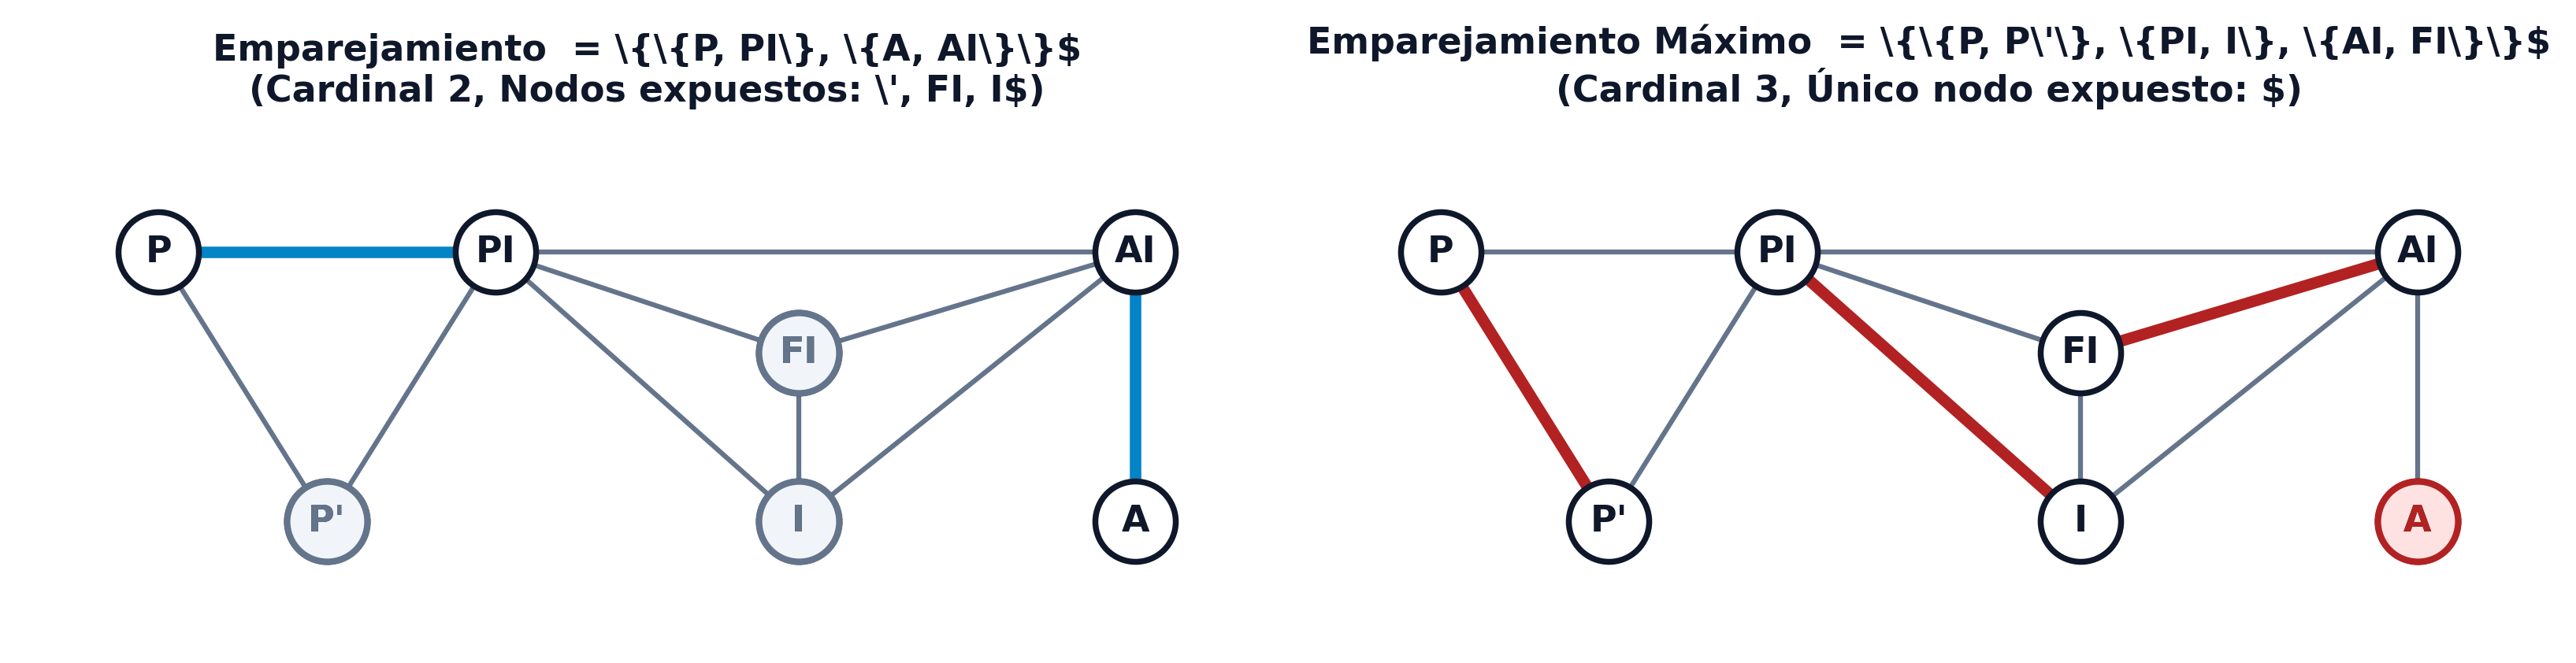
\includegraphics[width=0.9\linewidth,height=\textheight,keepaspectratio]{images/emparejamiento_tripulaciones_raf.png}

}

\caption{\label{fig-emparejamiento-tripulaciones-raf}Problema de
tripulaciones de la RAF: comparación entre un emparejamiento subóptimo
de 2 aristas (izquierda) y un emparejamiento máximo de 3 aristas
(derecha)}

\end{figure}%

Reorganizando las asignaciones hacia el emparejamiento
\(K_2 = \bigl\{ \{P, P'\}, \, \{PI, I\}, \, \{AI, FI\} \bigr\}\), se
logran formar \textbf{3 tripulaciones completas}, dejando únicamente al
piloto \(A\) sin pareja asignada. Dado que con \(7\) pilotos no es
posible formar más de \(3\) parejas independientes, \(K_2\) constituye
una solución de máxima cardinalidad.

\end{tcolorbox}

La formalización matemática de este problema requiere definir con
precisión los conceptos de aristas disjuntas, vértices saturados y
clases de optimalidad sobre grafos no dirigidos.

\begin{tcolorbox}[enhanced jigsaw, toprule=.15mm, opacitybacktitle=0.6, coltitle=black, colbacktitle=quarto-callout-note-color!10!white, title=\textcolor{quarto-callout-note-color}{\faInfo}\hspace{0.5em}{Definición: Emparejamiento en un grafo}, arc=.35mm, rightrule=.15mm, toptitle=1mm, breakable, bottomtitle=1mm, titlerule=0mm, colback=white, opacityback=0, leftrule=.75mm, colframe=quarto-callout-note-color-frame, left=2mm, bottomrule=.15mm]

Dado un grafo no dirigido simple \(G = (V, E)\), un
\textbf{emparejamiento} (o \emph{matching}) es un subconjunto de aristas
\(K \subseteq E\) tal que ninguna pareja de aristas en \(K\) comparte un
vértice en común, es decir:

\[
e_1 \cap e_2 = \emptyset, \quad \forall e_1, e_2 \in K, \; e_1 \neq e_2
\]

\end{tcolorbox}

Desde una perspectiva algebraica y de programación matemática, un
emparejamiento puede representarse mediante un vector binario de
decisión \(\mathbf{x} \in \{0, 1\}^{|E|}\), donde cada componente
\(x_e = 1\) si la arista \(e \in E\) se incluye en el emparejamiento y
\(x_e = 0\) en caso contrario. La condición de no adyacencia equivale a
imponer que, para cada vértice \(v \in V\), la suma de variables
incidentes no supere la unidad:

\[
\sum_{e \in \delta(v)} x_e \le 1, \quad \forall v \in V
\]

donde \(\delta(v)\) denota el conjunto de aristas incidentes en el
vértice \(v\). Esta estructura muestra que el conjunto de
emparejamientos es hereditario, propiedad clave que permite analizar
subconjuntos de soluciones válidas.

\begin{tcolorbox}[enhanced jigsaw, toprule=.15mm, opacitybacktitle=0.6, coltitle=black, colbacktitle=quarto-callout-note-color!10!white, title=\textcolor{quarto-callout-note-color}{\faInfo}\hspace{0.5em}{Proposición: Hereditariedad de los emparejamientos}, arc=.35mm, rightrule=.15mm, toptitle=1mm, breakable, bottomtitle=1mm, titlerule=0mm, colback=white, opacityback=0, leftrule=.75mm, colframe=quarto-callout-note-color-frame, left=2mm, bottomrule=.15mm]

Dado un grafo \(G = (V, E)\) y un emparejamiento \(K \subseteq E\),
cualquier subconjunto \(K' \subseteq K\) es también un emparejamiento de
\(G\).

\emph{Demostración}: Si \(K\) no contiene aristas con extremos
compartidos, la eliminación de una o más aristas para formar \(K'\)
preserva trivialmente la ausencia de aristas adyacentes.
\(\blacksquare\)

\end{tcolorbox}

La propiedad de hereditariedad implica que los emparejamientos forman
una familia de conjuntos independientes (un complejo simplicial o
sistema de independencia). Sobre esta familia, el objetivo primordial
consiste en encontrar la solución de mayor tamaño.

\begin{tcolorbox}[enhanced jigsaw, toprule=.15mm, opacitybacktitle=0.6, coltitle=black, colbacktitle=quarto-callout-note-color!10!white, title=\textcolor{quarto-callout-note-color}{\faInfo}\hspace{0.5em}{Definición: Problema de emparejamiento de máximo cardinal}, arc=.35mm, rightrule=.15mm, toptitle=1mm, breakable, bottomtitle=1mm, titlerule=0mm, colback=white, opacityback=0, leftrule=.75mm, colframe=quarto-callout-note-color-frame, left=2mm, bottomrule=.15mm]

Dado un grafo no dirigido \(G = (V, E)\), el \textbf{problema de
emparejamiento de máximo cardinal} consiste en determinar un
emparejamiento \(K \subseteq E\) que contenga el mayor número posible de
aristas, es decir, que maximice \(|K|\).

\end{tcolorbox}

Para caracterizar la calidad de una solución y guiar los algoritmos de
búsqueda, resulta esencial clasificar los vértices del grafo según su
pertenencia a las aristas del emparejamiento.

\begin{tcolorbox}[enhanced jigsaw, toprule=.15mm, opacitybacktitle=0.6, coltitle=black, colbacktitle=quarto-callout-note-color!10!white, title=\textcolor{quarto-callout-note-color}{\faInfo}\hspace{0.5em}{Definición: Vértices saturados y vértices expuestos}, arc=.35mm, rightrule=.15mm, toptitle=1mm, breakable, bottomtitle=1mm, titlerule=0mm, colback=white, opacityback=0, leftrule=.75mm, colframe=quarto-callout-note-color-frame, left=2mm, bottomrule=.15mm]

Dado un grafo \(G = (V, E)\) y un emparejamiento \(K \subseteq E\):

\begin{itemize}
\tightlist
\item
  Un vértice \(x \in V\) está \textbf{saturado} (o emparejado) por \(K\)
  si existe alguna arista \(\{x, y\} \in K\) incidente en \(x\).
\item
  Un vértice \(x \in V\) está \textbf{expuesto} (o no saturado, o libre)
  si ninguna arista de \(K\) incide en \(x\).
\end{itemize}

\end{tcolorbox}

Puesto que cada arista de \(K\) satura exactamente a \(2\) vértices
distintos y ningún vértice puede estar saturado por dos aristas a la
vez, el número total de vértices saturados por un emparejamiento \(K\)
es exactamente \(2|K|\), y el número de vértices expuestos es
\(|V| - 2|K|\).

Esta relación de conservación entre aristas y vértices conduce a una
cota superior natural: en cualquier grafo con \(n = |V|\) vértices, el
tamaño de cualquier emparejamiento está acotado por
\(|K| \le \lfloor n/2 \rfloor\). En consecuencia, cuando el número de
vértices libres se reduce al mínimo posible, la búsqueda algorítmica
concluye de forma inmediata.

\begin{tcolorbox}[enhanced jigsaw, toprule=.15mm, opacitybacktitle=0.6, coltitle=black, colbacktitle=quarto-callout-note-color!10!white, title=\textcolor{quarto-callout-note-color}{\faInfo}\hspace{0.5em}{Proposición: Condición de parada por cardinalidad de expuestos}, arc=.35mm, rightrule=.15mm, toptitle=1mm, breakable, bottomtitle=1mm, titlerule=0mm, colback=white, opacityback=0, leftrule=.75mm, colframe=quarto-callout-note-color-frame, left=2mm, bottomrule=.15mm]

Dado un grafo \(G = (V, E)\) con \(n = |V|\) vértices y un
emparejamiento \(K \subseteq E\), si el número de vértices no saturados
(expuestos) es \(0\) o \(1\), entonces \(K\) es un
\textbf{emparejamiento de máximo cardinal}.

\emph{Demostración}: Cualquier emparejamiento adicional requeriría
seleccionar al menos una arista no adyacente a las existentes, lo que
exige disponer de al menos \(2\) vértices no saturados disponibles. Al
haber como máximo \(1\) vértice libre, no es posible añadir ninguna
arista disjunta ni aumentar el cardinal. \(\blacksquare\)

\end{tcolorbox}

Es fundamental distinguir conceptualmente entre un
\textbf{emparejamiento maximal} (por inclusión) y un
\textbf{emparejamiento de máximo cardinal} (óptimo global):

\begin{itemize}
\tightlist
\item
  \textbf{Emparejamiento Maximal}: Es un emparejamiento al que no se le
  puede añadir ninguna arista adicional de \(E\) sin violar la condición
  de disyunción de vértices. Cualquier algoritmo codicioso
  (\emph{greedy}) encuentra un emparejamiento maximal rápidamente, pero
  este puede quedar atrapado en un óptimo local de cardinal
  estrictamente inferior al óptimo global (como ocurría en el
  emparejamiento \(K_1\) del problema de la RAF).
\item
  \textbf{Emparejamiento de Máximo Cardinal}: Es un emparejamiento que
  alcanza el máximo valor absoluto de \(|K|\) entre todos los
  emparejamientos posibles del grafo. Para transformar un emparejamiento
  maximal subóptimo en uno de máximo cardinal, es indispensable
  reorganizar y reasignar parejas a lo largo del grafo.
\end{itemize}

\begin{tcolorbox}[enhanced jigsaw, toprule=.15mm, opacitybacktitle=0.6, coltitle=black, colbacktitle=quarto-callout-note-color!10!white, title=\textcolor{quarto-callout-note-color}{\faInfo}\hspace{0.5em}{Definición: Emparejamiento perfecto}, arc=.35mm, rightrule=.15mm, toptitle=1mm, breakable, bottomtitle=1mm, titlerule=0mm, colback=white, opacityback=0, leftrule=.75mm, colframe=quarto-callout-note-color-frame, left=2mm, bottomrule=.15mm]

Dado un grafo \(G = (V, E)\) con \(n = |V|\) vértices, un emparejamiento
\(K \subseteq E\) se dice \textbf{perfecto} (o 1-factor) si satura a
todos los vértices del grafo (\(|V| - 2|K| = 0\)). En tal caso, el
tamaño del emparejamiento es exactamente:

\[
|K| = \frac{n}{2}
\]

lo que requiere necesariamente que el orden del grafo \(n\) sea un
número par.

\end{tcolorbox}

\section{Resolución mediante cadenas alternantes e
incrementales}\label{resoluciuxf3n-mediante-cadenas-alternantes-e-incrementales}

Para resolver de forma constructiva el problema de emparejamiento de
máximo cardinal cuando existen dos o más vértices expuestos, es
necesario analizar cómo modificar un emparejamiento existente para
incrementar su tamaño. En lugar de reconstruir el emparejamiento desde
cero, los métodos combinatorios emplean un principio de mejora local
iterativa basado en \textbf{cadenas alternantes de aristas}, que actúan
como cascadas de reasignación de parejas.

\subsection{Cadenas alternantes, cadenas incrementales y
transferencias}\label{cadenas-alternantes-cadenas-incrementales-y-transferencias}

La intuición física tras una cadena alternante reside en la posibilidad
de intercambiar las asignaciones actuales por nuevas parejas
compatibles. Al alternar aristas no emparejadas con aristas ya
emparejadas, cualquier cambio en una arista desencadena una reacción en
cadena que exige reajustar las aristas adyacentes.

\begin{tcolorbox}[enhanced jigsaw, toprule=.15mm, opacitybacktitle=0.6, coltitle=black, colbacktitle=quarto-callout-note-color!10!white, title=\textcolor{quarto-callout-note-color}{\faInfo}\hspace{0.5em}{Definición: Cadena alternante e incremental}, arc=.35mm, rightrule=.15mm, toptitle=1mm, breakable, bottomtitle=1mm, titlerule=0mm, colback=white, opacityback=0, leftrule=.75mm, colframe=quarto-callout-note-color-frame, left=2mm, bottomrule=.15mm]

Dado un grafo \(G = (V, E)\) y un emparejamiento \(K \subseteq E\):

\begin{itemize}
\tightlist
\item
  Una \textbf{cadena alternante} es una cadena simple
  \(\mu = (v_1, v_2, \dots, v_k)\) cuyas aristas pertenecen y no
  pertenecen alternativamente al emparejamiento \(K\) (es decir, las
  aristas alternan entre \(K\) y \(E \setminus K\)).
\item
  Una \textbf{cadena incremental} (o cadena de aumento) \(\mu[x, y]\)
  con \(x \neq y\) es una cadena alternante cuyos dos vértices extremos
  \(x\) e \(y\) son \textbf{vértices expuestos} (no saturados) respecto
  de \(K\).
\end{itemize}

\end{tcolorbox}

Las cadenas incrementales poseen propiedades algebraicas y combinatorias
muy definidas:

\begin{enumerate}
\def\labelenumi{\arabic{enumi}.}
\tightlist
\item
  \textbf{Longitud Impar de Aristas}: Toda cadena incremental contiene
  un \textbf{número impar de aristas}. Al comenzar y terminar en
  vértices no saturados, sus aristas primera y última deben pertenecer
  obligatoriamente a \(E \setminus K\).
\item
  \textbf{Balance de Aristas}: En una cadena incremental con \(2k + 1\)
  aristas, exactamente \(k + 1\) aristas pertenecen a \(E \setminus K\)
  y \(k\) aristas pertenecen a \(K\). El número de aristas fuera del
  emparejamiento supera siempre en una unidad al número de aristas
  dentro de \(K\).
\end{enumerate}

Esta asimetría en el número de aristas es la que permite incrementar el
tamaño global del emparejamiento mediante la operación de transferencia.

\begin{tcolorbox}[enhanced jigsaw, toprule=.15mm, opacitybacktitle=0.6, coltitle=black, colbacktitle=quarto-callout-note-color!10!white, title=\textcolor{quarto-callout-note-color}{\faInfo}\hspace{0.5em}{Definición: Operación de transferencia}, arc=.35mm, rightrule=.15mm, toptitle=1mm, breakable, bottomtitle=1mm, titlerule=0mm, colback=white, opacityback=0, leftrule=.75mm, colframe=quarto-callout-note-color-frame, left=2mm, bottomrule=.15mm]

Dado un emparejamiento \(K \subseteq E\) y una cadena incremental
\(\mu[x, y]\) respecto de \(K\), la \textbf{transferencia} consiste en
permutar la pertenencia de las aristas a lo largo de la cadena,
sustituyendo las aristas de \(\mu \cap K\) por las aristas de
\(\mu \setminus K\).

Algebraicamente, el nuevo emparejamiento \(K'\) se obtiene mediante la
\textbf{diferencia simétrica} (\(\bigtriangleup\)):

\[
K' = K \bigtriangleup \mu[x, y] = (K \setminus \mu) \cup (\mu \setminus K)
\]

El emparejamiento resultante satisface estrictamente:

\[
|K'| = |K| + 1
\]

\end{tcolorbox}

La operación de transferencia preserva de manera rigurosa la validez del
emparejamiento: en los vértices interiores de la cadena \(\mu\), la
arista eliminada de \(K\) es reemplazada exactamente por una nueva
arista incidente en dicho vértice, manteniendo su grado saturado en
\(1\). En los dos vértices extremos \(x\) e \(y\), que antes estaban
expuestos, la incorporación de las aristas extremas pasa su estado a
saturado (\(sat = 1\)), incrementando el cardinal total en una unidad
sin alterar el estado del resto del grafo.

\begin{tcolorbox}[enhanced jigsaw, toprule=.15mm, opacitybacktitle=0.6, coltitle=black, colbacktitle=quarto-callout-tip-color!10!white, title=\textcolor{quarto-callout-tip-color}{\faLightbulb}\hspace{0.5em}{Ejemplo: Aplicación de una transferencia en un grafo de 6 nodos}, arc=.35mm, rightrule=.15mm, toptitle=1mm, breakable, bottomtitle=1mm, titlerule=0mm, colback=white, opacityback=0, leftrule=.75mm, colframe=quarto-callout-tip-color-frame, left=2mm, bottomrule=.15mm]

Considérese el grafo de 6 vértices \(V = \{1, 2, 3, 4, 5, 6\}\) y 9
aristas
\(E = \bigl\{ \{1,2\}, \{1,3\}, \{2,3\}, \{2,5\}, \{3,4\}, \{3,6\}, \{4,5\}, \{4,6\}, \{5,6\} \bigr\}\)
presentado en la Figura~\ref{fig-cadenas-alternantes-transferencia}.

Partimos del emparejamiento inicial
\(K = \bigl\{ \{2,3\}, \, \{5,6\} \bigr\}\) con \(|K| = 2\). Evaluamos
la red:

\begin{enumerate}
\def\labelenumi{\arabic{enumi}.}
\tightlist
\item
  \textbf{Identificación de Vértices Expuestos}: Los vértices
  \(2, 3, 5, 6\) están saturados por \(K\). Los vértices \(1\) y \(4\)
  son vértices expuestos (\(1, 4 \notin V(K)\)).
\item
  \textbf{Detección de la Cadena Incremental}: La trayectoria
  \(\mu = (1, 2, 3, 4)\) une los vértices expuestos \(1\) y \(4\). Sus
  aristas son:

  \begin{itemize}
  \tightlist
  \item
    \(\{1, 2\} \notin K\) (fuera de \(K\))
  \item
    \(\{2, 3\} \in K\) (dentro de \(K\))
  \item
    \(\{3, 4\} \notin K\) (fuera de \(K\)) La cadena alterna aristas de
    \(E \setminus K\) y \(K\), y tiene longitud \(3\) (impar).
  \end{itemize}
\item
  \textbf{Ejecución de la Transferencia}: Calculamos la diferencia
  simétrica \(K' = K \bigtriangleup \mu\):

  \begin{itemize}
  \tightlist
  \item
    Eliminamos la arista \(\{2, 3\} \in K\).
  \item
    Incorporamos las aristas \(\{1, 2\}\) y \(\{3, 4\}\).
  \item
    Mantenemos la arista ajena a la cadena \(\{5, 6\}\).
  \end{itemize}

  Obtenemos el nuevo emparejamiento: \[
  K' = \bigl\{ \{1,2\}, \, \{3,4\}, \, \{5,6\} \bigr\}
  \] El cardinal aumenta de \(|K| = 2\) a \(|K'| = 3\). Dado que
  \(|K'| = 6/2 = 3\), \(K'\) satura a todos los vértices del grafo y
  constituye un \textbf{emparejamiento perfecto}.
\end{enumerate}

\begin{figure}[H]

\centering{

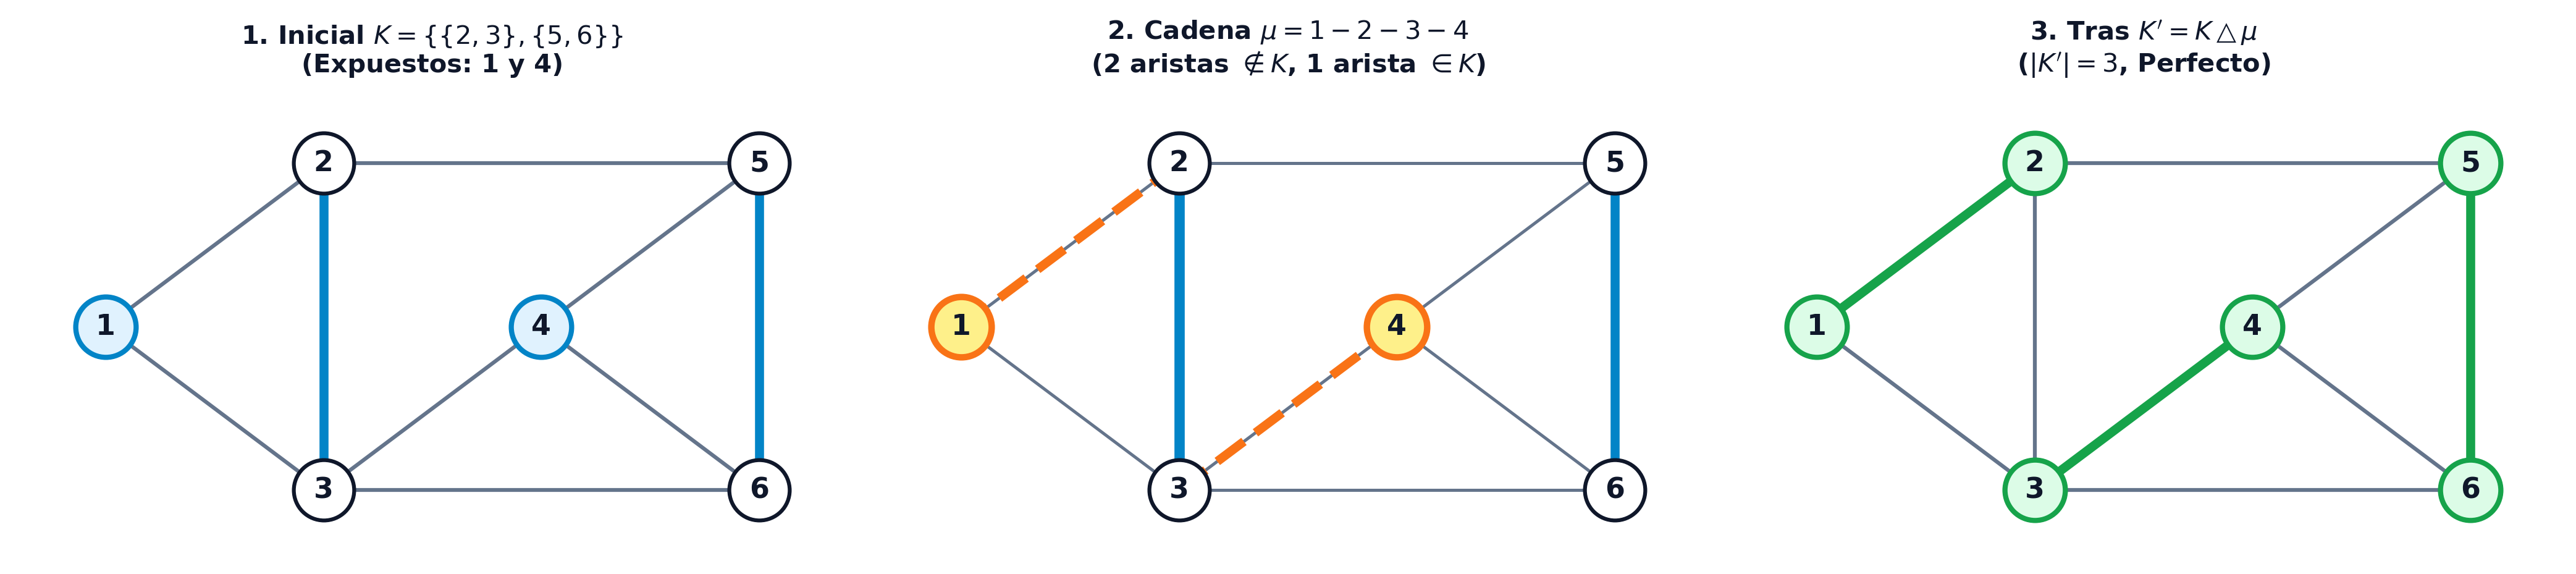
\includegraphics[width=0.95\linewidth,height=\textheight,keepaspectratio]{images/cadenas_alternantes_transferencia.png}

}

\caption{\label{fig-cadenas-alternantes-transferencia}Proceso de
transferencia: estado inicial \(K\) (izquierda), identificación de la
cadena incremental (centro) y nuevo emparejamiento \(K'\) (derecha)}

\end{figure}%

\end{tcolorbox}

\subsection{Teorema de caracterización de Berge y descomposición de
componentes}\label{teorema-de-caracterizaciuxf3n-de-berge-y-descomposiciuxf3n-de-componentes}

La relación directa entre las cadenas incrementales y el aumento del
cardinal conduce a la caracterización fundamental de optimalidad
descubierta por Claude Berge en 1957 (Berge 1957). Para demostrar este
teorema formalmente, es necesario caracterizar previamente la estructura
topológica que surge al superponer dos emparejamientos distintos sobre
un mismo grafo.

Al calcular la diferencia simétrica \(K_1 \bigtriangleup K_2\) entre dos
emparejamientos \(K_1\) y \(K_2\), estamos aislando el \textbf{grafo de
discrepancias} entre ambas soluciones.

\begin{tcolorbox}[enhanced jigsaw, toprule=.15mm, opacitybacktitle=0.6, coltitle=black, colbacktitle=quarto-callout-note-color!10!white, title=\textcolor{quarto-callout-note-color}{\faInfo}\hspace{0.5em}{Lema: Estructura del grafo diferencia simétrica}, arc=.35mm, rightrule=.15mm, toptitle=1mm, breakable, bottomtitle=1mm, titlerule=0mm, colback=white, opacityback=0, leftrule=.75mm, colframe=quarto-callout-note-color-frame, left=2mm, bottomrule=.15mm]

Dados dos emparejamientos cualesquiera \(K_1\) y \(K_2\) en un grafo
simple \(G = (V, E)\), el subgrafo parcial generado por la diferencia
simétrica \(G' = (V, K_1 \bigtriangleup K_2)\) está compuesto
exclusivamente por componentes conexas disjuntas que pertenecen a alguno
de los siguientes tres tipos:

\begin{enumerate}
\def\labelenumi{\arabic{enumi}.}
\tightlist
\item
  \textbf{Vértices aislados} (grado \(0\)).
\item
  \textbf{Ciclos elementales alternantes} de longitud estrictamente par
  (cuyas aristas alternan entre \(K_1\) y \(K_2\)).
\item
  \textbf{Cadenas elementales alternantes} de longitud par o impar
  (cuyas aristas alternan entre \(K_1\) y \(K_2\)).
\end{enumerate}

\emph{Demostración}: Analicemos el grado máximo que puede tener
cualquier vértice \(v \in V\) en el grafo diferencia
\(G' = (V, K_1 \bigtriangleup K_2)\):

\begin{itemize}
\tightlist
\item
  \textbf{Caso 1 (Vértice no saturado por \(K_1\) ni por \(K_2\))}:
  Ninguna arista de \(K_1 \cup K_2\) incide en \(v\). Por tanto, el
  grado de \(v\) en \(G'\) es \(d_{G'}(v) = 0\) (vértice aislado).
\item
  \textbf{Caso 2 (Vértice saturado por \(K_1\) y por \(K_2\) con la
  misma arista)}: Sea \(e \in K_1 \cap K_2\) la arista incidente. Por
  definición de diferencia simétrica,
  \(e \notin K_1 \bigtriangleup K_2\). Ninguna otra arista de \(K_1\) ni
  de \(K_2\) incide en \(v\), luego \(d_{G'}(v) = 0\) (vértice aislado).
\item
  \textbf{Caso 3 (Vértice saturado sólo por uno de los dos
  emparejamientos)}: Si \(v\) está saturado por \(e_1 \in K_1\) y
  ninguna arista de \(K_2\) incide en \(v\) (o viceversa), entonces
  exactamente una arista incidente pertenece a
  \(K_1 \bigtriangleup K_2\), por lo que \(d_{G'}(v) = 1\). Estos
  vértices corresponden exclusivamente a los extremos de cadenas
  alternantes.
\item
  \textbf{Caso 4 (Vértice saturado por ambos emparejamientos con aristas
  distintas)}: Si \(e_1 \in K_1\) y \(e_2 \in K_2\) con \(e_1 \neq e_2\)
  inciden en \(v\), ambas aristas pertenecen a
  \(K_1 \bigtriangleup K_2\). Al no poder incidir más de una arista de
  cada emparejamiento en \(v\), el grado es exactamente
  \(d_{G'}(v) = 2\).
\end{itemize}

Puesto que ningún vértice en \(G'\) tiene grado superior a \(2\)
(\(d_{G'}(v) \le 2, \forall v \in V\)), todo grafo de grado máximo 2 se
descompone de forma unívoca en vértices aislados, cadenas simples y
ciclos cerrados. Además, como las aristas deben alternar estrictamente
entre \(K_1\) y \(K_2\), los ciclos cerrados deben cerrarse alternando
aristas de ambos conjuntos, lo que exige obligatoriamente un número par
de aristas. \(\blacksquare\)

\end{tcolorbox}

Como se ilustra en la Figura~\ref{fig-lema-diferencia-componentes} y en
la Figura~\ref{fig-lema-diferencia-bipartito}, el lema anterior permite
descomponer cualquier par de soluciones en piezas estructurales
elementales independientes sin ramificaciones complejas.

\begin{figure}

\centering{

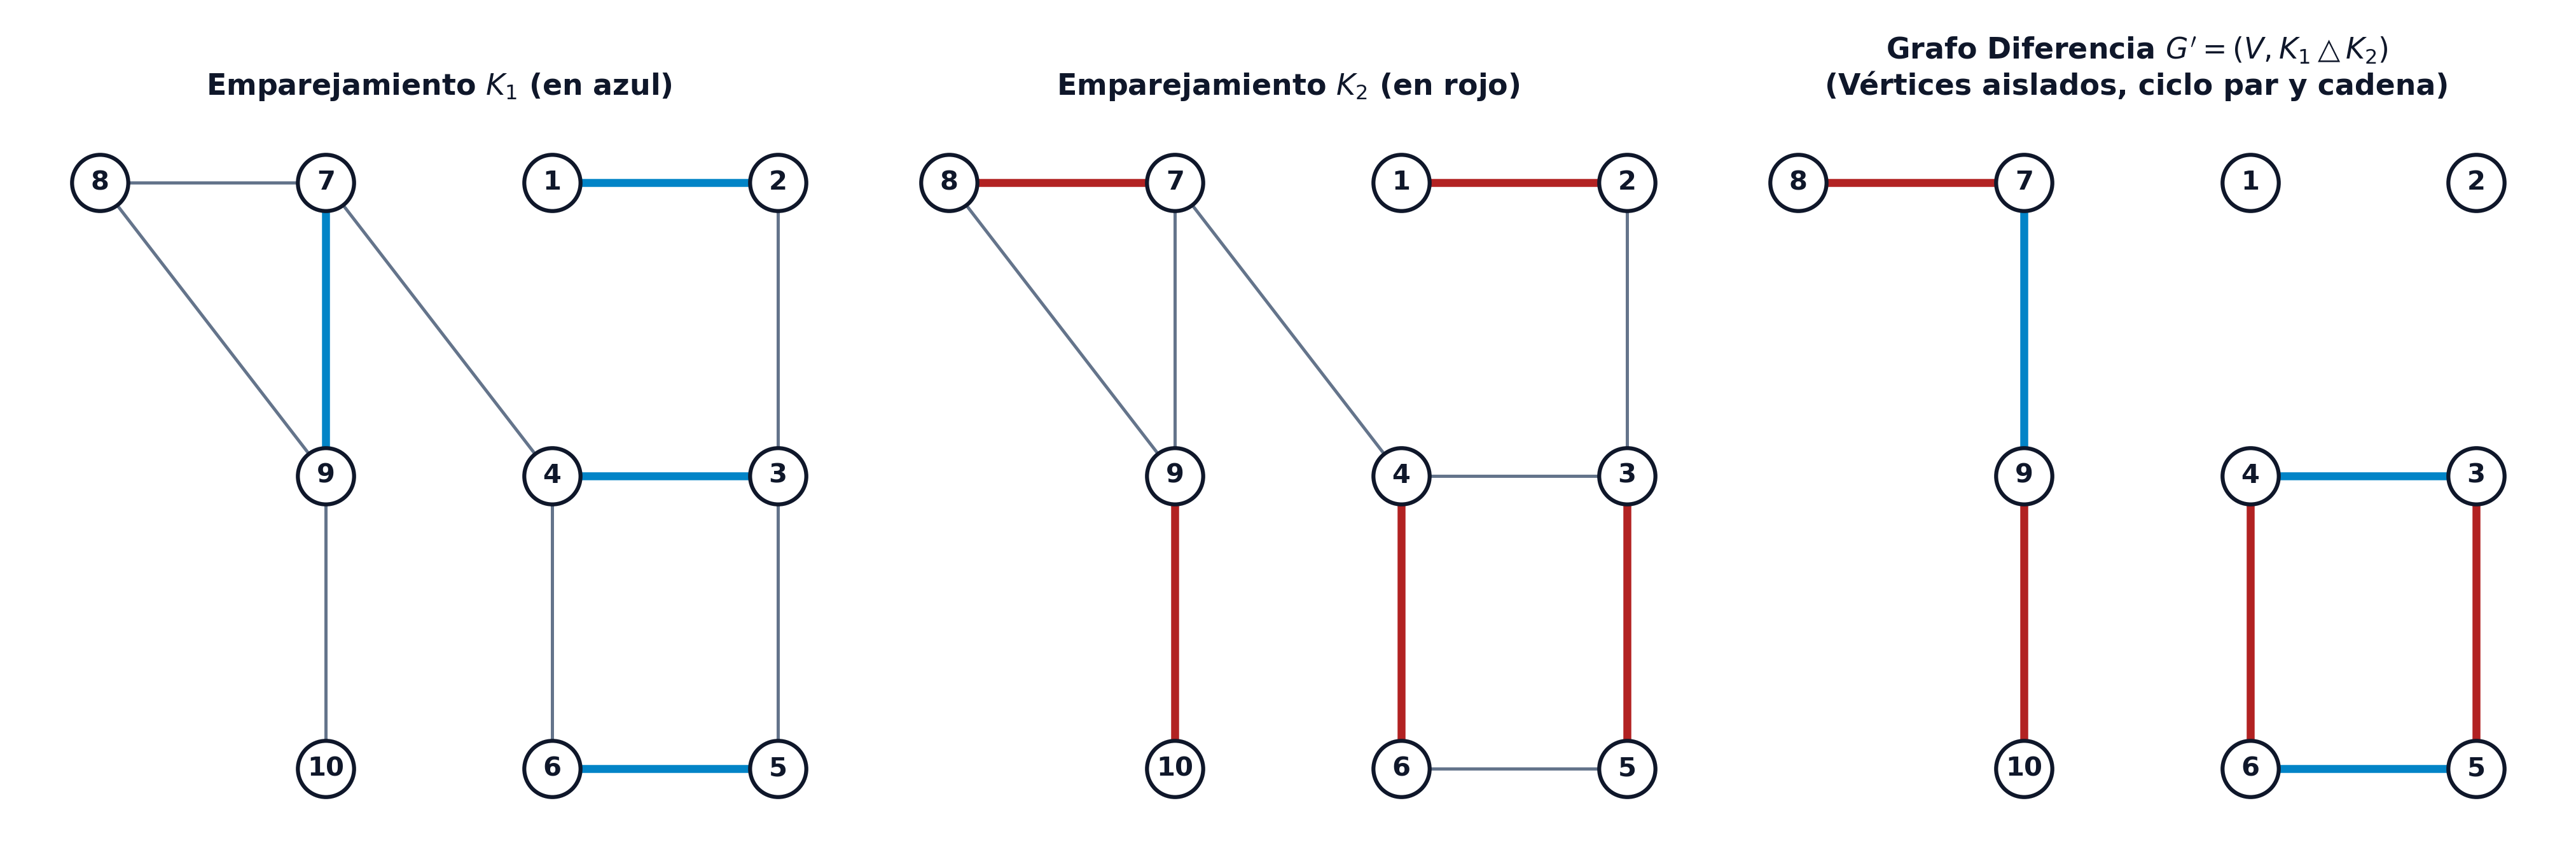
\includegraphics[width=0.95\linewidth,height=\textheight,keepaspectratio]{images/lema_diferencia_simetrica_componentes.png}

}

\caption{\label{fig-lema-diferencia-componentes}Descomposición del grafo
diferencia simétrica \(G' = (V, K_1 \bigtriangleup K_2)\) en vértices
aislados, ciclos pares y cadenas alternantes}

\end{figure}%

\begin{figure}

\centering{

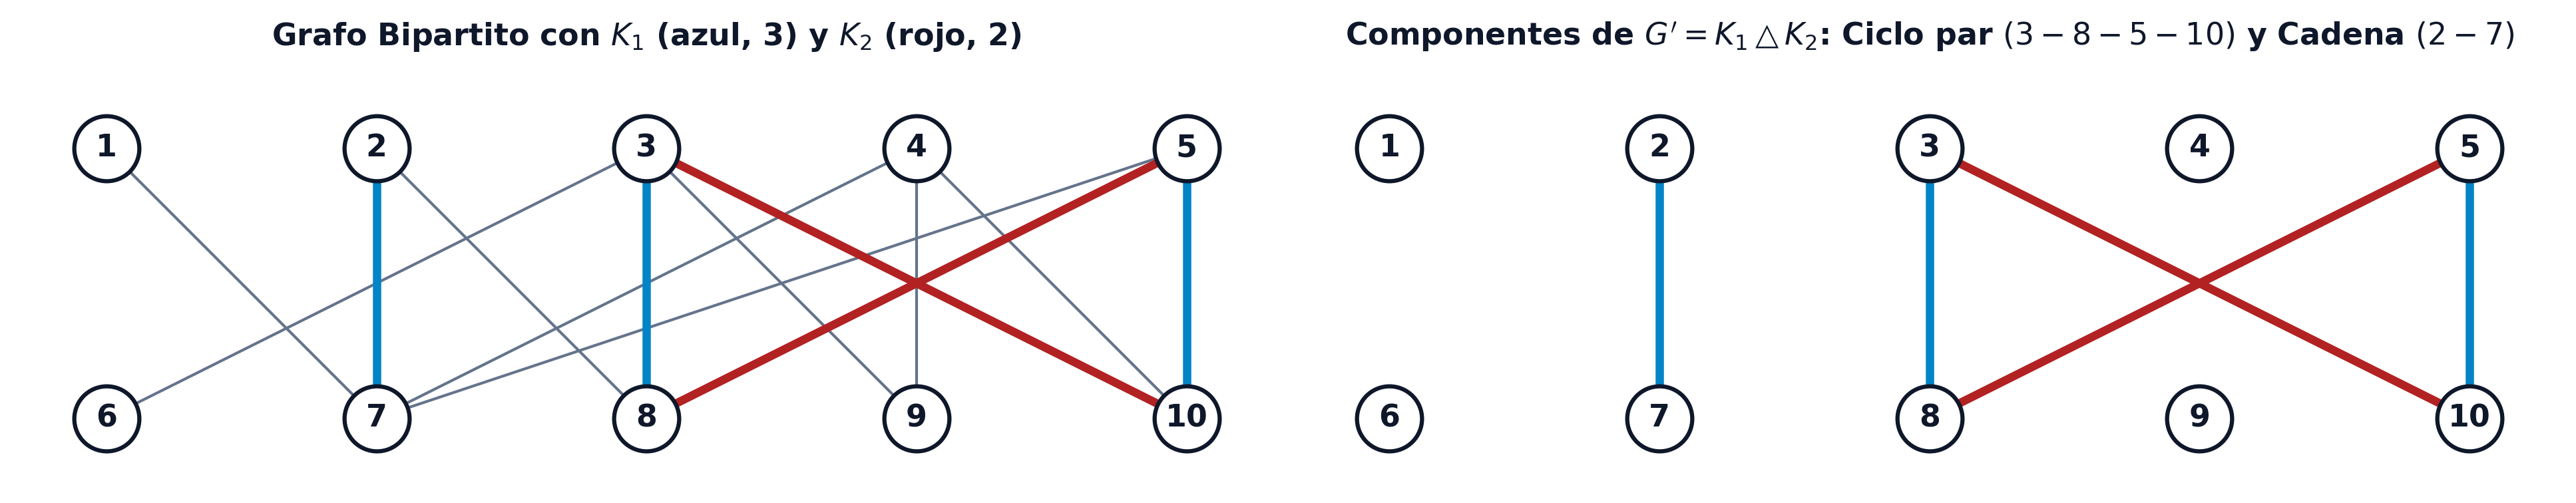
\includegraphics[width=0.9\linewidth,height=\textheight,keepaspectratio]{images/lema_diferencia_bipartito_ejemplo.png}

}

\caption{\label{fig-lema-diferencia-bipartito}Evaluación de la
diferencia simétrica \(K_1 \bigtriangleup K_2\) sobre un grafo bipartito
de 10 vértices}

\end{figure}%

A partir del lema de descomposición de la diferencia simétrica, podemos
demostrar de forma rigurosa el Teorema de Berge.

\begin{tcolorbox}[enhanced jigsaw, toprule=.15mm, opacitybacktitle=0.6, coltitle=black, colbacktitle=quarto-callout-important-color!10!white, title=\textcolor{quarto-callout-important-color}{\faExclamation}\hspace{0.5em}{Teorema de caracterización de Berge (1957)}, arc=.35mm, rightrule=.15mm, toptitle=1mm, breakable, bottomtitle=1mm, titlerule=0mm, colback=white, opacityback=0, leftrule=.75mm, colframe=quarto-callout-important-color-frame, left=2mm, bottomrule=.15mm]

Dado un grafo \(G = (V, E)\), un emparejamiento \(K \subseteq E\) es de
\textbf{máximo cardinal} si y solo si el grafo \(G\) \textbf{no contiene
ninguna cadena incremental} con respecto a \(K\).

\emph{Demostración}: Demostramos la doble implicación:

\begin{itemize}
\tightlist
\item
  \textbf{Necesidad (\(\implies\))}: Razonamos por reducción al absurdo.
  Supongamos que \(K\) es de máximo cardinal y que existe una cadena
  incremental \(\mu[x, y]\) respecto de \(K\). Aplicando la operación de
  transferencia, el nuevo conjunto \(K' = K \bigtriangleup \mu[x, y]\)
  es un emparejamiento válido de \(G\) con cardinal
  \(|K'| = |K| + 1 > |K|\), lo que contradice la hipótesis de que \(K\)
  era de cardinal máximo.
\item
  \textbf{Suficiencia (\(\impliedby\))}: Supongamos que \(K\) no
  contiene ninguna cadena incremental respecto de sí mismo. Sea \(K^*\)
  un emparejamiento de máximo cardinal en \(G\) (cuya existencia está
  garantizada al ser el conjunto de aristas finito). Consideramos el
  subgrafo diferencia simétrica \(G' = (V, K \bigtriangleup K^*)\).
\end{itemize}

Por el Lema de Descomposición, \(G'\) se compone únicamente de vértices
aislados, ciclos pares alternantes y cadenas alternantes:

\begin{enumerate}
\def\labelenumi{\arabic{enumi}.}
\tightlist
\item
  Los vértices aislados contienen \(0\) aristas de \(K\) y \(0\) de
  \(K^*\).
\item
  Cada ciclo alternante contiene exactamente el mismo número de aristas
  de \(K\) que de \(K^*\) (al tener longitud par).
\item
  En cada cadena alternante de longitud par, el número de aristas de
  \(K\) iguala al de \(K^*\).
\item
  En cada cadena alternante de longitud impar, las aristas alternan
  comenzando y terminando con el mismo emparejamiento. Si alguna cadena
  impar tuviera más aristas de \(K^*\) que de \(K\), sus extremos serían
  vértices no saturados por \(K\), lo que convertiría a dicha cadena en
  una \textbf{cadena incremental respecto de \(K\)}. Pero por hipótesis,
  \(K\) no admite cadenas incrementales. Por tanto, ninguna cadena impar
  puede tener más aristas de \(K^*\) que de \(K\).
\end{enumerate}

Sumando el número de aristas en todas las componentes conexas de \(G'\),
se deduce que \(|K^*| \le |K|\). Dado que por definición de máximo
\(|K| \le |K^*|\), concluimos que \(|K| = |K^*|\), lo que certifica que
\(K\) es de máximo cardinal. \(\blacksquare\)

\end{tcolorbox}

El Teorema de Berge constituye la piedra angular de la teoría de
emparejamientos y juega un papel análogo al \textbf{Teorema de Flujo
Máximo - Corte Mínimo de Ford-Fulkerson} en redes de transporte (donde
la ausencia de caminos de aumento en la red residual certifica el flujo
máximo, como se vio en el Capítulo 8) y al criterio de parada del
\textbf{método del Símplex} en Programación Lineal (donde la no
negatividad de los costes reducidos certifica la optimalidad global,
como se demostró en el Capítulo 3). En todos estos casos, una condición
de optimalidad local determinista certifica la optimalidad global
absoluta.

\section{Algoritmo del árbol alternante y contracción de flores
(Edmonds)}\label{algoritmo-del-uxe1rbol-alternante-y-contracciuxf3n-de-flores-edmonds}

El Teorema de Berge reduce el problema de optimización a una tarea
constructiva: buscar de forma sistemática cadenas incrementales en el
grafo o certificar formalmente que no existen. Para realizar esta
búsqueda de manera determinista y eficiente, se utiliza la estructura
jerárquica del \textbf{árbol alternante}.

\subsection{Estructura del bosque y árbol
alternante}\label{estructura-del-bosque-y-uxe1rbol-alternante}

Dado un emparejamiento \(K\) y un vértice expuesto, el objetivo
algorítmico consiste en explorar caminos alternantes en busca de una
cadena incremental de longitud impar que termine en otro vértice
expuesto. Para formular este proceso, identificamos el estado de cada
vértice \(x \in V\) mediante una \textbf{variable indicadora de
saturación}:

\[
sat(x) = \begin{cases} 1, & \text{si } x \text{ está saturado por } K \text{ (existe } e \in K \text{ incidente en } x) \\ 0, & \text{si } x \text{ es un vértice expuesto o no saturado} \end{cases}
\]

\begin{tcolorbox}[enhanced jigsaw, toprule=.15mm, opacitybacktitle=0.6, coltitle=black, colbacktitle=quarto-callout-note-color!10!white, title=\textcolor{quarto-callout-note-color}{\faInfo}\hspace{0.5em}{Nota: Bipartición del subgrafo de aristas del emparejamiento}, arc=.35mm, rightrule=.15mm, toptitle=1mm, breakable, bottomtitle=1mm, titlerule=0mm, colback=white, opacityback=0, leftrule=.75mm, colframe=quarto-callout-note-color-frame, left=2mm, bottomrule=.15mm]

A partir de cualquier emparejamiento \(K\) sobre un grafo general
\(G = (V, E)\) (sea este originalmente bipartito o no), el subgrafo
parcial \(G_K = (V, K)\) formado exclusivamente por las aristas de \(K\)
es siempre un \textbf{grafo bipartito}. En efecto, al ser las aristas de
\(K\) disjuntas en vértices, cada arista forma una componente conexa
\(K_2\) independiente, cuyos dos extremos pueden asignarse a conjuntos
disjuntos de una bipartición.

\end{tcolorbox}

\begin{tcolorbox}[enhanced jigsaw, toprule=.15mm, opacitybacktitle=0.6, coltitle=black, colbacktitle=quarto-callout-note-color!10!white, title=\textcolor{quarto-callout-note-color}{\faInfo}\hspace{0.5em}{Definición: Árbol alternante y bosque alternante}, arc=.35mm, rightrule=.15mm, toptitle=1mm, breakable, bottomtitle=1mm, titlerule=0mm, colback=white, opacityback=0, leftrule=.75mm, colframe=quarto-callout-note-color-frame, left=2mm, bottomrule=.15mm]

Dados un grafo \(G = (V, E)\) y un emparejamiento \(K \subseteq E\), un
\textbf{árbol alternante} es un subgrafo parcial \(H = (W, T)\) con
\(W \subseteq V\) y \(T \subseteq E\) que satisface las siguientes tres
propiedades fundamentales:

\begin{enumerate}
\def\labelenumi{\arabic{enumi}.}
\tightlist
\item
  \(H\) es un árbol (subgrafo conexo y sin ciclos).
\item
  Existe un único vértice distinguido \(r \in W\), denominado
  \textbf{raíz del árbol alternante}, que es un vértice expuesto
  respecto del emparejamiento \(K\) (\(sat(r) = 0\)).
\item
  Cualquier cadena elemental en \(H\) que une un vértice cualquiera
  \(w \in W\) con la raíz \(r\) es una \textbf{cadena alternante}.
\end{enumerate}

Un conjunto de árboles alternantes disjuntos cuyas raíces son vértices
expuestos de \(G\) constituye un \textbf{bosque alternante}. Cada árbol
se denota unívocamente a partir de su raíz mediante
\(H(r) = (W(r), T(r))\).

\end{tcolorbox}

Para la gestión y navegación computacional del bosque alternante, se
emplea el \textbf{vector de antecesores o vector de padres}
\(\mathbf{p} = (p(1), p(2), \dots, p(n))^T \in V^n\). Cada raíz
\(r \in R\) de un árbol alternante se identifica de forma unívoca por la
autorreferencia \(p(r) = r\). La única cadena alternante que conecta
cualquier vértice \(w \in W(r)\) con su raíz \(r\) se recupera de manera
determinista encadenando las referencias del vector \(\mathbf{p}\):

\[
w \longleftrightarrow p(w) \longleftrightarrow p(p(w)) \longleftrightarrow \cdots \longleftrightarrow p(\cdots(p(w))\cdots) \longleftrightarrow r
\]

\begin{tcolorbox}[enhanced jigsaw, toprule=.15mm, opacitybacktitle=0.6, coltitle=black, colbacktitle=quarto-callout-tip-color!10!white, title=\textcolor{quarto-callout-tip-color}{\faLightbulb}\hspace{0.5em}{Ejemplo: Bosque alternante y verificación de maximalidad en grafo de 6
nodos}, arc=.35mm, rightrule=.15mm, toptitle=1mm, breakable, bottomtitle=1mm, titlerule=0mm, colback=white, opacityback=0, leftrule=.75mm, colframe=quarto-callout-tip-color-frame, left=2mm, bottomrule=.15mm]

Considérese el grafo de 6 vértices \(V = \{1, 2, 3, 4, 5, 6\}\) y
aristas
\(E = \bigl\{ \{1,4\}, \{1,5\}, \{1,6\}, \{2,5\}, \{3,5\} \bigr\}\)
representado en la Figura~\ref{fig-arbol-ejemplo-6nodos}, con el
emparejamiento inicial \(K = \bigl\{ \{1,4\}, \, \{2,5\} \bigr\}\).

\begin{enumerate}
\def\labelenumi{\arabic{enumi}.}
\item
  \textbf{Identificación de Raíces}: Los vértices saturados son
  \(\{1, 2, 4, 5\}\) (\(sat = 1\)), mientras que los vértices expuestos
  son \(\{3, 6\}\) (\(sat = 0\)). Por tanto, el conjunto de raíces del
  bosque alternante es \(R = \{3, 6\}\).
\item
  \textbf{Construcción de los Árboles Alternantes}:

  \begin{itemize}
  \item
    Árbol \(H(3) = (W(3), T(3))\) con raíz \(r = 3\):
    \[W(3) = \{2, 3, 5\}, \quad T(3) = \bigl\{ \{3,5\}, \, \{2,5\} \bigr\}\]
  \item
    Árbol \(H(6) = (W(6), T(6))\) con raíz \(r = 6\):
    \[W(6) = \{1, 4, 6\}, \quad T(6) = \bigl\{ \{6,1\}, \, \{1,4\} \bigr\}\]
  \end{itemize}
\item
  \textbf{Vector de Padres}: El vector de antecesores queda determinado
  por: \[
  \mathbf{p}^T = (6, 5, 3, 1, 3, 6)
  \]
\item
  \textbf{Conclusión de Optimalidad}: Desde los árboles alternantes no
  es posible alcanzar ningún otro vértice expuesto mediante aristas
  alternantes. Al no existir cadenas incrementales, el Teorema de Berge
  certifica que \(K\) es un \textbf{emparejamiento de máximo cardinal}
  (\(|K| = 2\)).
\end{enumerate}

\begin{figure}[H]

\centering{

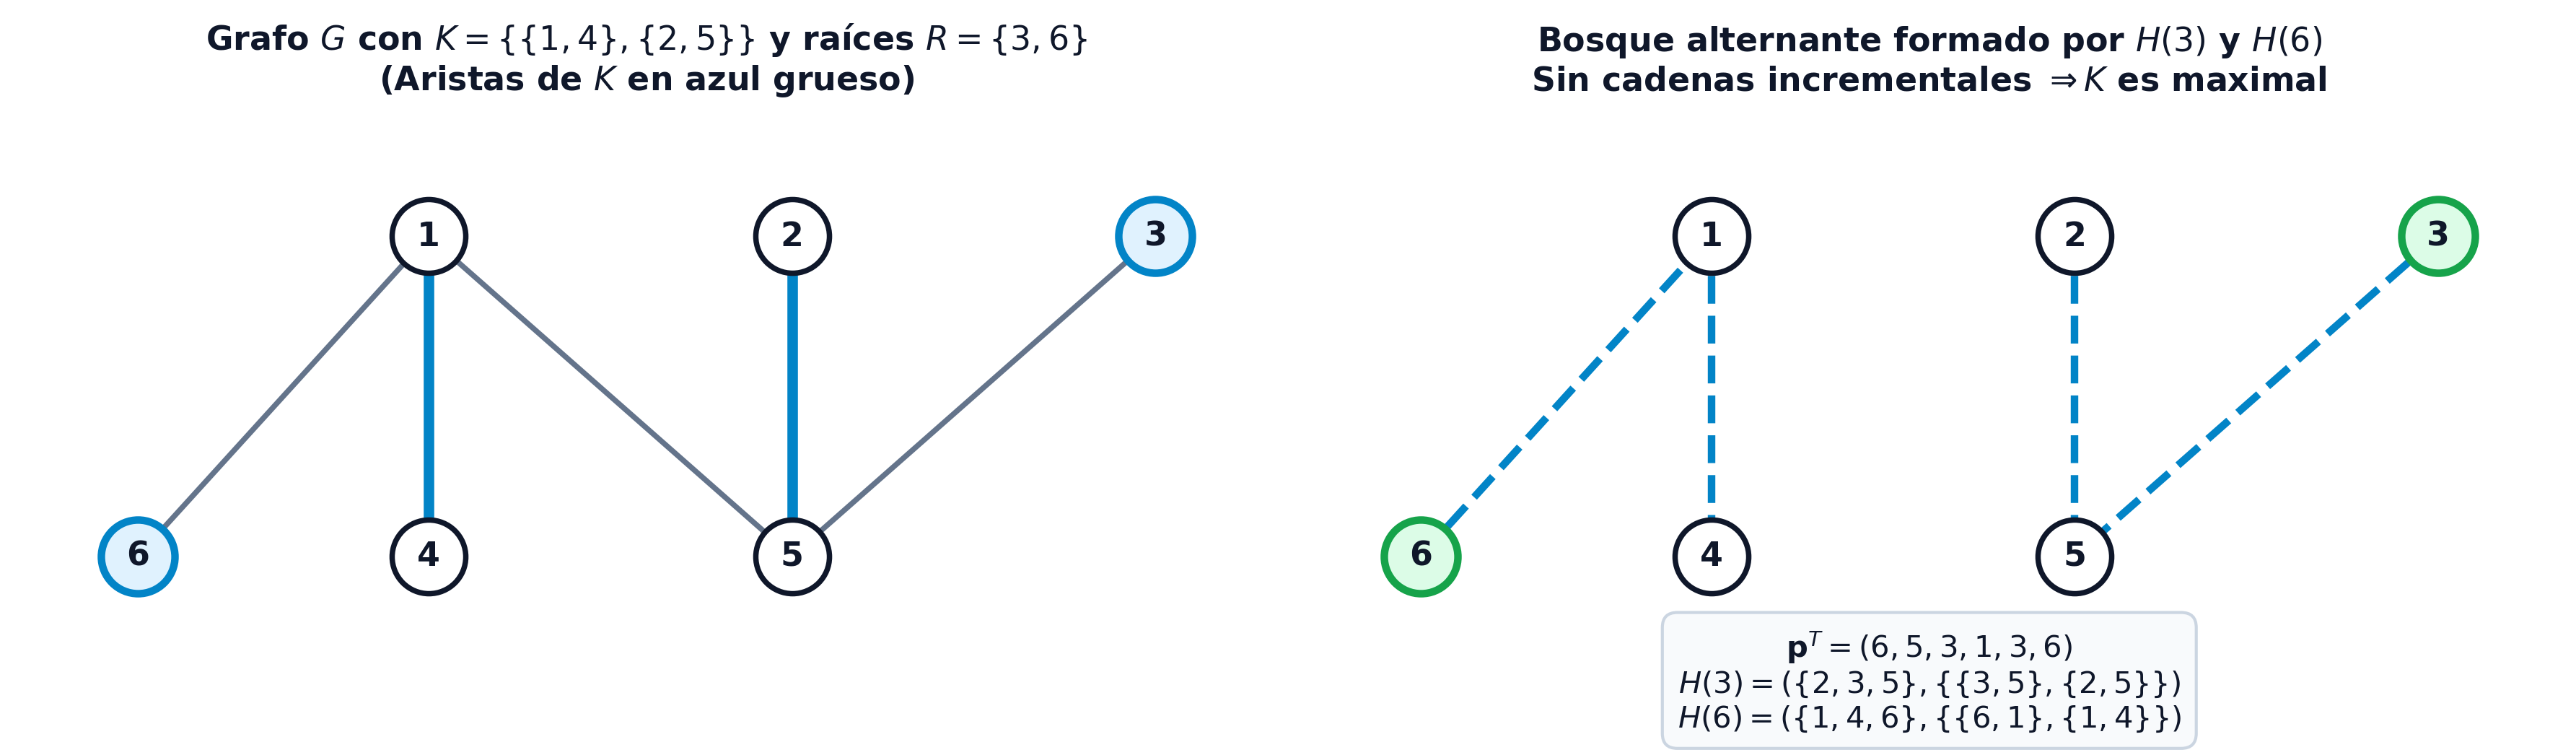
\includegraphics[width=0.9\linewidth,height=\textheight,keepaspectratio]{images/arbol_alternante_ejemplo_6nodos.png}

}

\caption{\label{fig-arbol-ejemplo-6nodos}Bosque alternante en grafo de 6
nodos: configuración inicial de \(K\) (izq.) y descomposición en árboles
\(H(3)\) y \(H(6)\) caracterizados por el vector \(\mathbf{p}\) (der.)}

\end{figure}%

\end{tcolorbox}

Cuando la exploración del árbol alternante sí alcanza otros vértices
expuestos antes de agotarse, se descubre al menos una cadena incremental
que permite aplicar la transferencia y aumentar el cardinal del
emparejamiento, como se detalla en el siguiente ejemplo:

\begin{tcolorbox}[enhanced jigsaw, toprule=.15mm, opacitybacktitle=0.6, coltitle=black, colbacktitle=quarto-callout-tip-color!10!white, title=\textcolor{quarto-callout-tip-color}{\faLightbulb}\hspace{0.5em}{Ejemplo: Detección de cadenas incrementales y transferencia en grafo
bipartito de 10 nodos}, arc=.35mm, rightrule=.15mm, toptitle=1mm, breakable, bottomtitle=1mm, titlerule=0mm, colback=white, opacityback=0, leftrule=.75mm, colframe=quarto-callout-tip-color-frame, left=2mm, bottomrule=.15mm]

Considérese el grafo bipartito de 10 vértices \(V = \{1, \dots, 10\}\)
ilustrado en la Figura~\ref{fig-arbol-ejemplo-10nodos}, con el
emparejamiento inicial
\(K_1 = \bigl\{ \{2,7\}, \, \{3,8\}, \, \{5,10\} \bigr\}\) de cardinal
\(3\).

\begin{enumerate}
\def\labelenumi{\arabic{enumi}.}
\item
  \textbf{Inicialización del Árbol con Raíz Expuesta}: El nodo \(1\) es
  un vértice expuesto (\(sat(1) = 0\)). Tomamos \(R = \{1\}\) como raíz
  del árbol alternante.
\item
  \textbf{Vector de Padres}: Tras explorar las aristas del grafo
  bipartito desde la raíz \(1\) (alcanzando el camino alternante
  \(1 \to 7 \to 2 \to 8 \to 3\) y, desde el vértice \(3\), ramificando
  hacia los nodos \(6\), \(9\) y la rama \(10 \to 5\)), el vector de
  antecesores obtenido es: \[
  \mathbf{p}^T = (1, 7, 8, 0, 10, 3, 1, 2, 3, 3)
  \] donde \(p(4) = 0\) indica que el nodo \(4\) no es alcanzado por el
  árbol, mientras que \(p(10) = 3\) y \(p(5) = 10\) caracterizan la
  exploración de la rama saturada \(\{5, 10\}\).
\item
  \textbf{Identificación de Cadenas Incrementales}: Los vértices \(6\) y
  \(9\) son vértices expuestos que han sido alcanzados por el árbol.
  Desenrollando sus antecesores mediante \(\mathbf{p}\), obtenemos dos
  cadenas incrementales que conectan con la raíz \(1\): \[
  6 \longleftrightarrow p(6)=3 \longleftrightarrow p(3)=8 \longleftrightarrow p(8)=2 \longleftrightarrow p(2)=7 \longleftrightarrow p(7)=1
  \] \[
  9 \longleftrightarrow p(9)=3 \longleftrightarrow p(3)=8 \longleftrightarrow p(8)=2 \longleftrightarrow p(2)=7 \longleftrightarrow p(7)=1
  \]
\item
  \textbf{Ejecución de la Transferencia}: Aplicando la transferencia por
  la cadena incremental que parte del nodo expuesto \(6\): \[
  \mu = (6, 3, 8, 2, 7, 1)
  \] Calculamos la diferencia simétrica
  \(K'_1 = K_1 \bigtriangleup \mu\): \[
  K'_1 = \bigl\{ \{6,3\}, \, \{8,2\}, \, \{7,1\}, \, \{5,10\} \bigr\}
  \] El cardinal resultante aumenta a \(|K'_1| = 4\), logrando un nuevo
  emparejamiento con una arista adicional.
\end{enumerate}

\begin{figure}[H]

\centering{

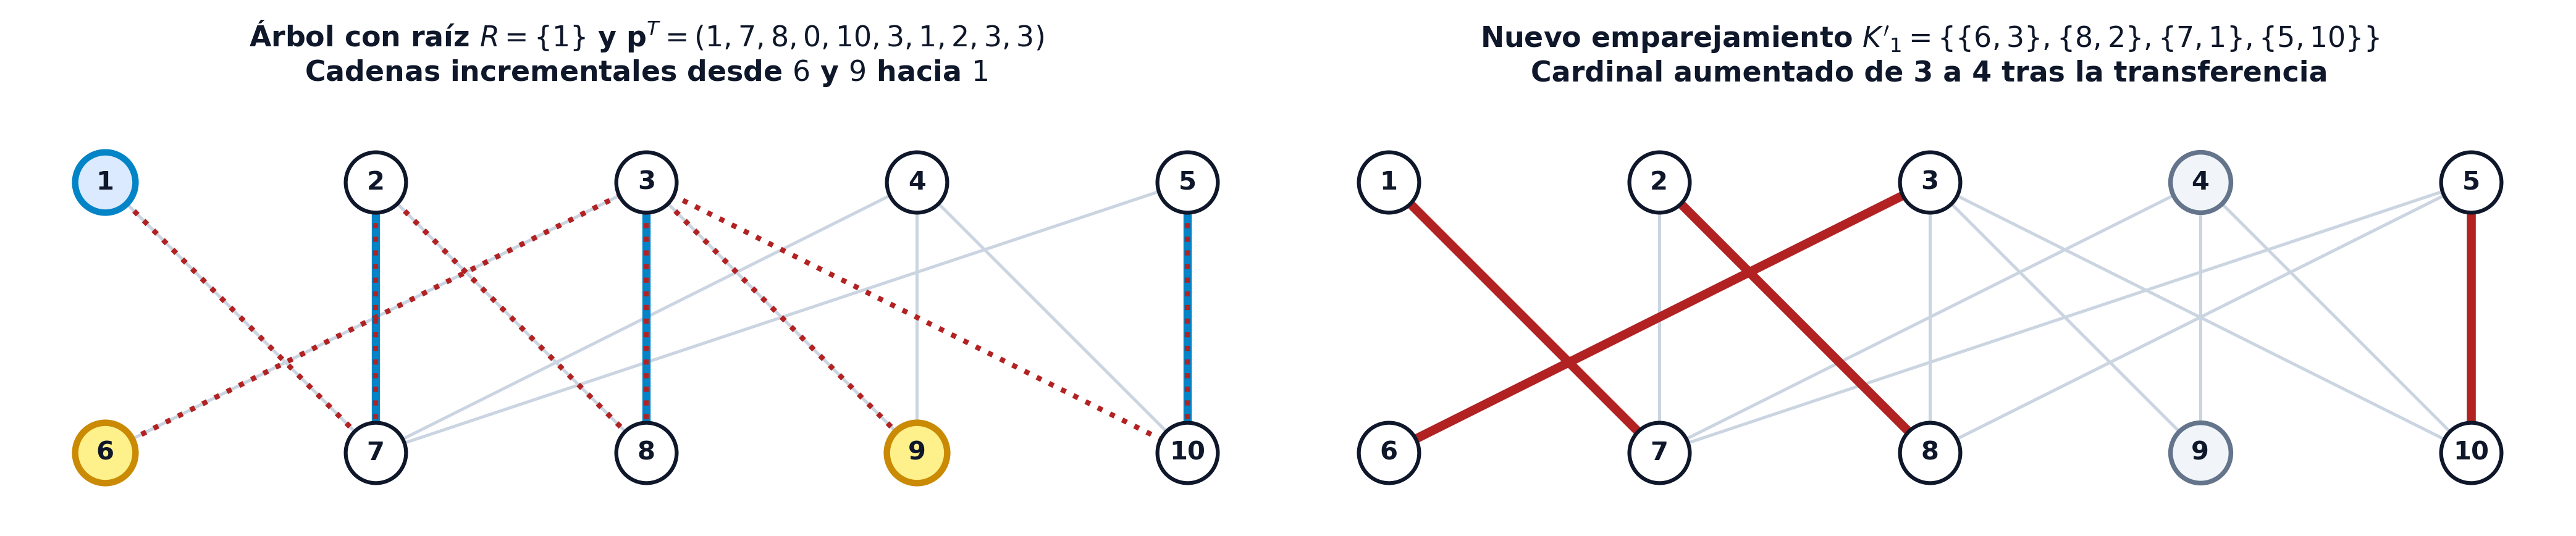
\includegraphics[width=0.95\linewidth,height=\textheight,keepaspectratio]{images/arbol_alternante_ejemplo_10nodos.png}

}

\caption{\label{fig-arbol-ejemplo-10nodos}Búsqueda mediante árbol
alternante en grafo de 10 nodos: identificación de cadenas incrementales
desde los nodos expuestos \(6\) y \(9\) (izq.) y nuevo emparejamiento
aumentado \(K'_1\) tras la transferencia (der.)}

\end{figure}%

\end{tcolorbox}

\subsection{El desafío de los ciclos impares y la contracción de flores
de
Edmonds}\label{el-desafuxedo-de-los-ciclos-impares-y-la-contracciuxf3n-de-flores-de-edmonds}

En grafos bipartitos, todos los ciclos tienen longitud par, lo que
garantiza que la búsqueda mediante árboles alternantes siempre progresa
de forma directa hacia nuevos vértices o detecta cadenas incrementales.
Sin embargo, en grafos generales no bipartitos, la presencia de
\textbf{ciclos de longitud impar} (denominados \emph{flores} o
\emph{blossoms}) introduce una dificultad estructural profunda.

Como se ilustra en la Figura~\ref{fig-contraccion-ciclo-flor}, en un
ciclo impar de \(2k + 1\) vértices (por ejemplo, el ciclo de 5 vértices
\(C_5\)), el emparejamiento maximal dentro del ciclo puede saturar como
máximo a \(2k\) vértices mediante \(k\) aristas, dejando exactamente
\textbf{un vértice expuesto}. La propiedad algebraica y combinatoria
clave de la flor es que \textbf{cualquiera de los \(2k+1\) vértices del
ciclo puede elegirse libremente como el vértice expuesto}, mientras los
restantes \(2k\) vértices quedan completamente saturados por parejas
disjuntas.

\begin{figure}

\centering{

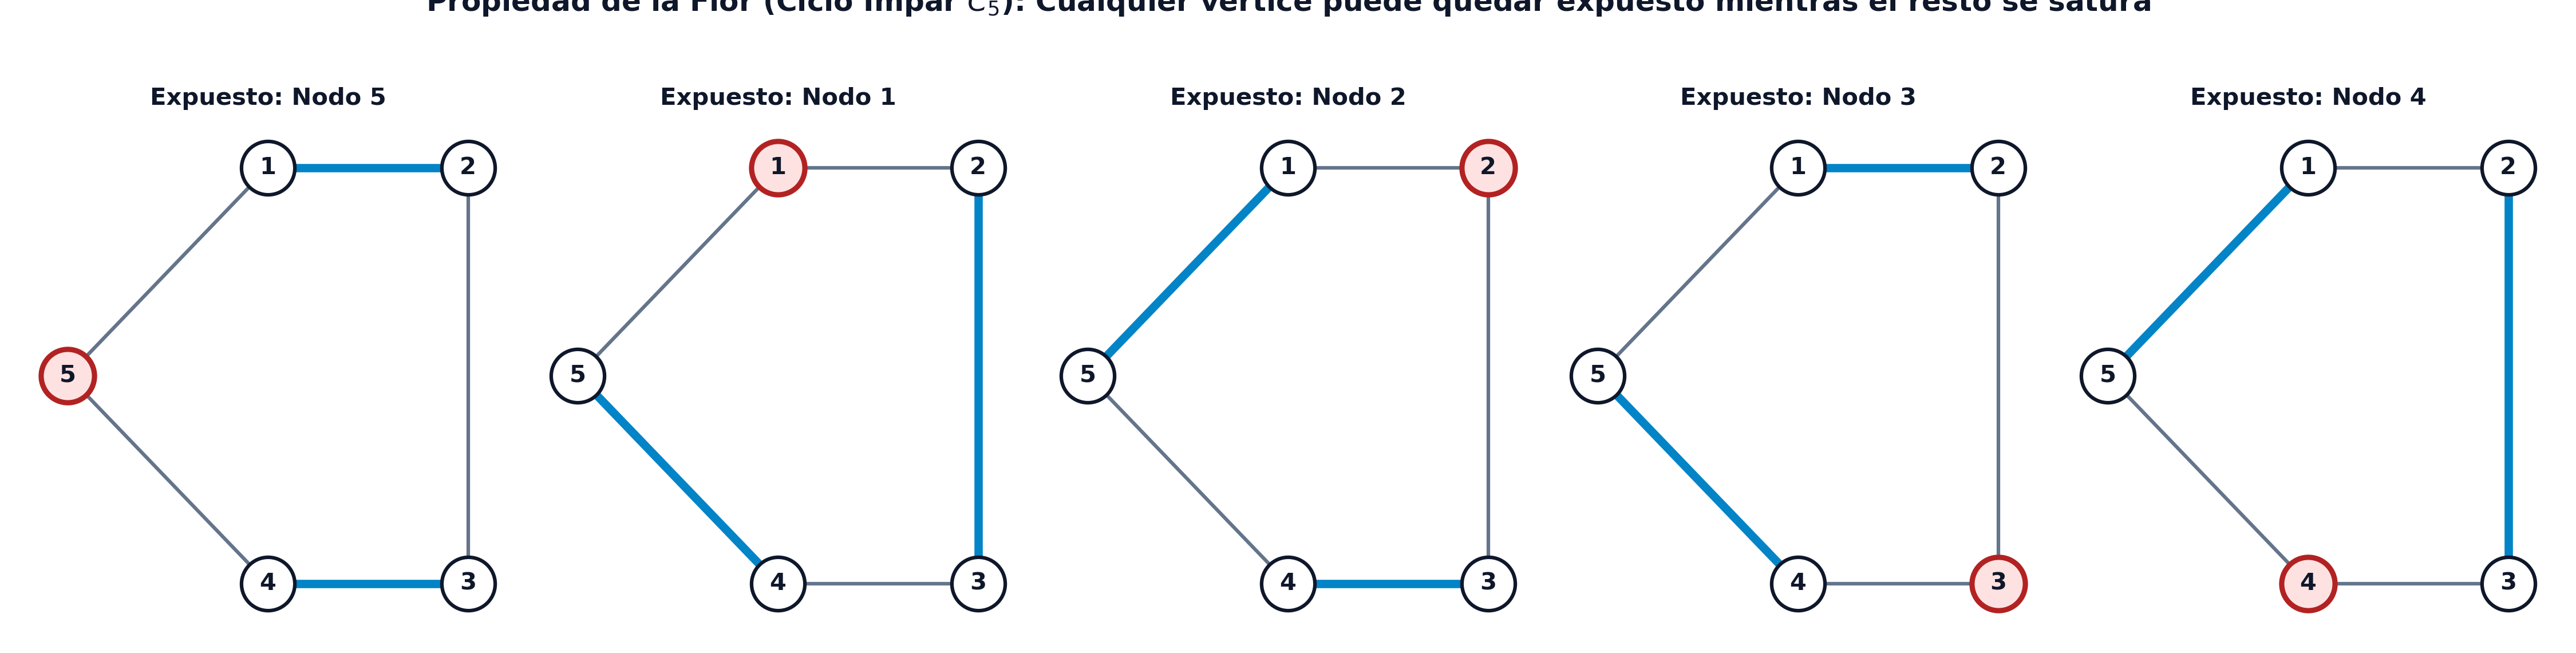
\includegraphics[width=0.95\linewidth,height=\textheight,keepaspectratio]{images/contraccion_ciclo_impar_flor.png}

}

\caption{\label{fig-contraccion-ciclo-flor}Propiedad de la flor en un
ciclo impar \(C_5\): cualquiera de sus 5 vértices puede quedar expuesto
mientras los 4 restantes quedan saturados}

\end{figure}%

Para sortear este obstáculo sin explorar factorialmente todas las
posibles asignaciones internas del ciclo, Jack Edmonds introdujo en 1965
la técnica de \textbf{contracción de flores}: comprimir todo el ciclo
impar en un único pseudovértice (\emph{supernodo}) \(w\), resolver el
emparejamiento en el grafo comprimido, y descontraer (\emph{expandir})
posteriormente el ciclo ajustando internamente las aristas (Edmonds
1965).

\begin{tcolorbox}[enhanced jigsaw, toprule=.15mm, opacitybacktitle=0.6, coltitle=black, colbacktitle=quarto-callout-note-color!10!white, title=\textcolor{quarto-callout-note-color}{\faInfo}\hspace{0.5em}{Definición: Contracción de un grafo (Grafo comprimido)}, arc=.35mm, rightrule=.15mm, toptitle=1mm, breakable, bottomtitle=1mm, titlerule=0mm, colback=white, opacityback=0, leftrule=.75mm, colframe=quarto-callout-note-color-frame, left=2mm, bottomrule=.15mm]

Dado un grafo no dirigido \(G = (V, E)\) y un subconjunto de vértices
\(W \subset V\) correspondiente a un ciclo impar, se define el
\textbf{grafo comprimido} \(G/W\) como:

\[
G/W = \bigl( (V \setminus W) \cup \{w\}, \, E/W \bigr)
\]

donde \(w\) es un nuevo pseudovértice representativo y el conjunto de
aristas \(E/W\) se define como:

\[
E/W = \bigl\{ \{i, j\} \in E \mid i, j \notin W \bigr\} \cup \bigl\{ \{w, j\} \mid \exists i \in W \text{ tal que } \{i, j\} \in E, \, j \notin W \bigr\}
\]

\end{tcolorbox}

El siguiente resultado teórico, formulado por Jack Edmonds, garantiza
que la contracción de un ciclo impar preserva la capacidad de
reconstruir un emparejamiento válido sobre el grafo original mediante
una descompresión determinista.

\begin{tcolorbox}[enhanced jigsaw, toprule=.15mm, opacitybacktitle=0.6, coltitle=black, colbacktitle=quarto-callout-important-color!10!white, title=\textcolor{quarto-callout-important-color}{\faExclamation}\hspace{0.5em}{Teorema: Contracción de ciclos impares de Edmonds (1965)}, arc=.35mm, rightrule=.15mm, toptitle=1mm, breakable, bottomtitle=1mm, titlerule=0mm, colback=white, opacityback=0, leftrule=.75mm, colframe=quarto-callout-important-color-frame, left=2mm, bottomrule=.15mm]

Sea \(G = (V, E)\) un grafo, \(W \subset V\) un subconjunto de vértices
asociado a un ciclo de longitud impar, y sea \(K_1\) un emparejamiento
en el grafo comprimido \(G/W\).

Entonces, existe un emparejamiento \(K_W\) en el subgrafo generado por
\(W\) tal que:

\[
K = K_1 \cup K_W
\]

es un emparejamiento válido de \(G\).

\emph{Demostración}: Al ser \(W\) un ciclo de longitud impar
\(|W| = 2k + 1\), el emparejamiento maximal \(K_W\) dentro de \(W\)
contiene \(k\) aristas y deja exactamente un vértice \(v \in W\) sin
saturar. Distinguimos dos situaciones posibles sobre el pseudovértice
\(w\) en el emparejamiento \(K_1\):

\begin{enumerate}
\def\labelenumi{\arabic{enumi}.}
\tightlist
\item
  Si \(w\) está expuesto en \(K_1\), se selecciona cualquier
  emparejamiento \(K_W\) de \(k\) aristas en \(W\). El único nodo de
  \(W\) que queda sin saturar actúa como vértice expuesto en \(G\), y
  ningún arco de \(K_1\) interfiere con \(W\), por lo que
  \(K = K_1 \cup K_W\) es un emparejamiento válido.
\item
  Si \(w\) está saturado en \(K_1\) por una arista \(\{w, j\} \in K_1\),
  dicha arista proviene originalmente de una arista \(\{i, j\} \in E\)
  con \(i \in W\) y \(j \notin W\). En tal caso, seleccionamos en \(W\)
  el emparejamiento \(K_W\) de \(k\) aristas que deja precisamente al
  vértice \(i\) como el único nodo no saturado de \(W\). De este modo,
  la arista \(\{i, j\}\) satura a \(i\) desde el exterior, y las \(k\)
  aristas de \(K_W\) saturan a los restantes \(2k\) vértices de \(W\).
  Como ninguna otra arista de \(K_1\) incide en \(W\),
  \(K = (K_1 \setminus \{\{w, j\}\}) \cup \{\{i, j\}\} \cup K_W\) es un
  emparejamiento válido en \(G\). \(\blacksquare\)
\end{enumerate}

\end{tcolorbox}

\begin{tcolorbox}[enhanced jigsaw, toprule=.15mm, opacitybacktitle=0.6, coltitle=black, colbacktitle=quarto-callout-note-color!10!white, title=\textcolor{quarto-callout-note-color}{\faInfo}\hspace{0.5em}{Nota: Reglas pedagógicas de descompresión de flores}, arc=.35mm, rightrule=.15mm, toptitle=1mm, breakable, bottomtitle=1mm, titlerule=0mm, colback=white, opacityback=0, leftrule=.75mm, colframe=quarto-callout-note-color-frame, left=2mm, bottomrule=.15mm]

Las claves operativas de la contracción de flores se resumen en tres
principios:

\begin{itemize}
\tightlist
\item
  \textbf{Existencia de vértice expuesto}: Al ser \(W\) un ciclo impar,
  siempre queda exactamente un vértice no saturado en \(W\) respecto de
  \(K_W\).
\item
  \textbf{Libertad de selección del vértice expuesto}: Siempre es
  posible elegir de forma determinista qué vértice del ciclo queda no
  saturado.
\item
  \textbf{Alineación con la arista exterior}: Si el pseudovértice \(w\)
  está saturado en \(K_1\), se deja como no saturado en el ciclo
  precisamente el vértice \(i \in W\) incidente en la arista exterior
  que satura a \(w\), asegurando que ningún vértice del ciclo quede
  saturado dos veces.
\end{itemize}

\end{tcolorbox}

A pesar de la elegancia del Teorema de Edmonds, la contracción de flores
debe gestionarse con extrema cautela dentro de un esquema algorítmico
formal, ya que operar directamente con maximalidades en el grafo
comprimido puede conducir a soluciones subóptimas:

\begin{tcolorbox}[enhanced jigsaw, toprule=.15mm, opacitybacktitle=0.6, coltitle=black, colbacktitle=quarto-callout-warning-color!10!white, title=\textcolor{quarto-callout-warning-color}{\faExclamationTriangle}\hspace{0.5em}{Advertencia: Maximalidad en grafos comprimidos}, arc=.35mm, rightrule=.15mm, toptitle=1mm, breakable, bottomtitle=1mm, titlerule=0mm, colback=white, opacityback=0, leftrule=.75mm, colframe=quarto-callout-warning-color-frame, left=2mm, bottomrule=.15mm]

Que un emparejamiento \(K_1\) sea \textbf{maximal} en el grafo
comprimido \(G/W\) no implica necesariamente que el emparejamiento
extendido \(K\) sea de \textbf{máximo cardinal} en el grafo original
\(G\).

Como se ilustra en la Figura~\ref{fig-contraejemplo-maximalidad},
considérese un grafo con un ciclo impar \(\{1, 2, 3\}\) y tres aristas
exteriores \(\{ \{1,6\}, \{2,4\}, \{3,5\} \}\). Al comprimir el ciclo
\(\{1, 2, 3\}\) en el pseudonodo \(w\), el grafo comprimido \(G/W\)
contiene las aristas \(\{ \{w,6\}, \{w,4\}, \{w,5\} \}\). El
emparejamiento \(K_1 = \bigl\{ \{w, 6\} \bigr\}\) es maximal en \(G/W\)
(no puede añadirse ninguna otra arista disjunta), pero produce en \(G\)
un emparejamiento de cardinal \(2\)
(\(K = \bigl\{ \{1,6\}, \{2,3\} \bigr\}\)), cuando el grafo original
admite el emparejamiento de cardinal \(3\):
\(K^* = \bigl\{ \{1,6\}, \{2,4\}, \{3,5\} \bigr\}\). Por esta razón, la
contracción debe ejecutarse guiada estrictamente por la jerarquía de
niveles del árbol alternante de Edmonds.

\begin{figure}[H]

\centering{

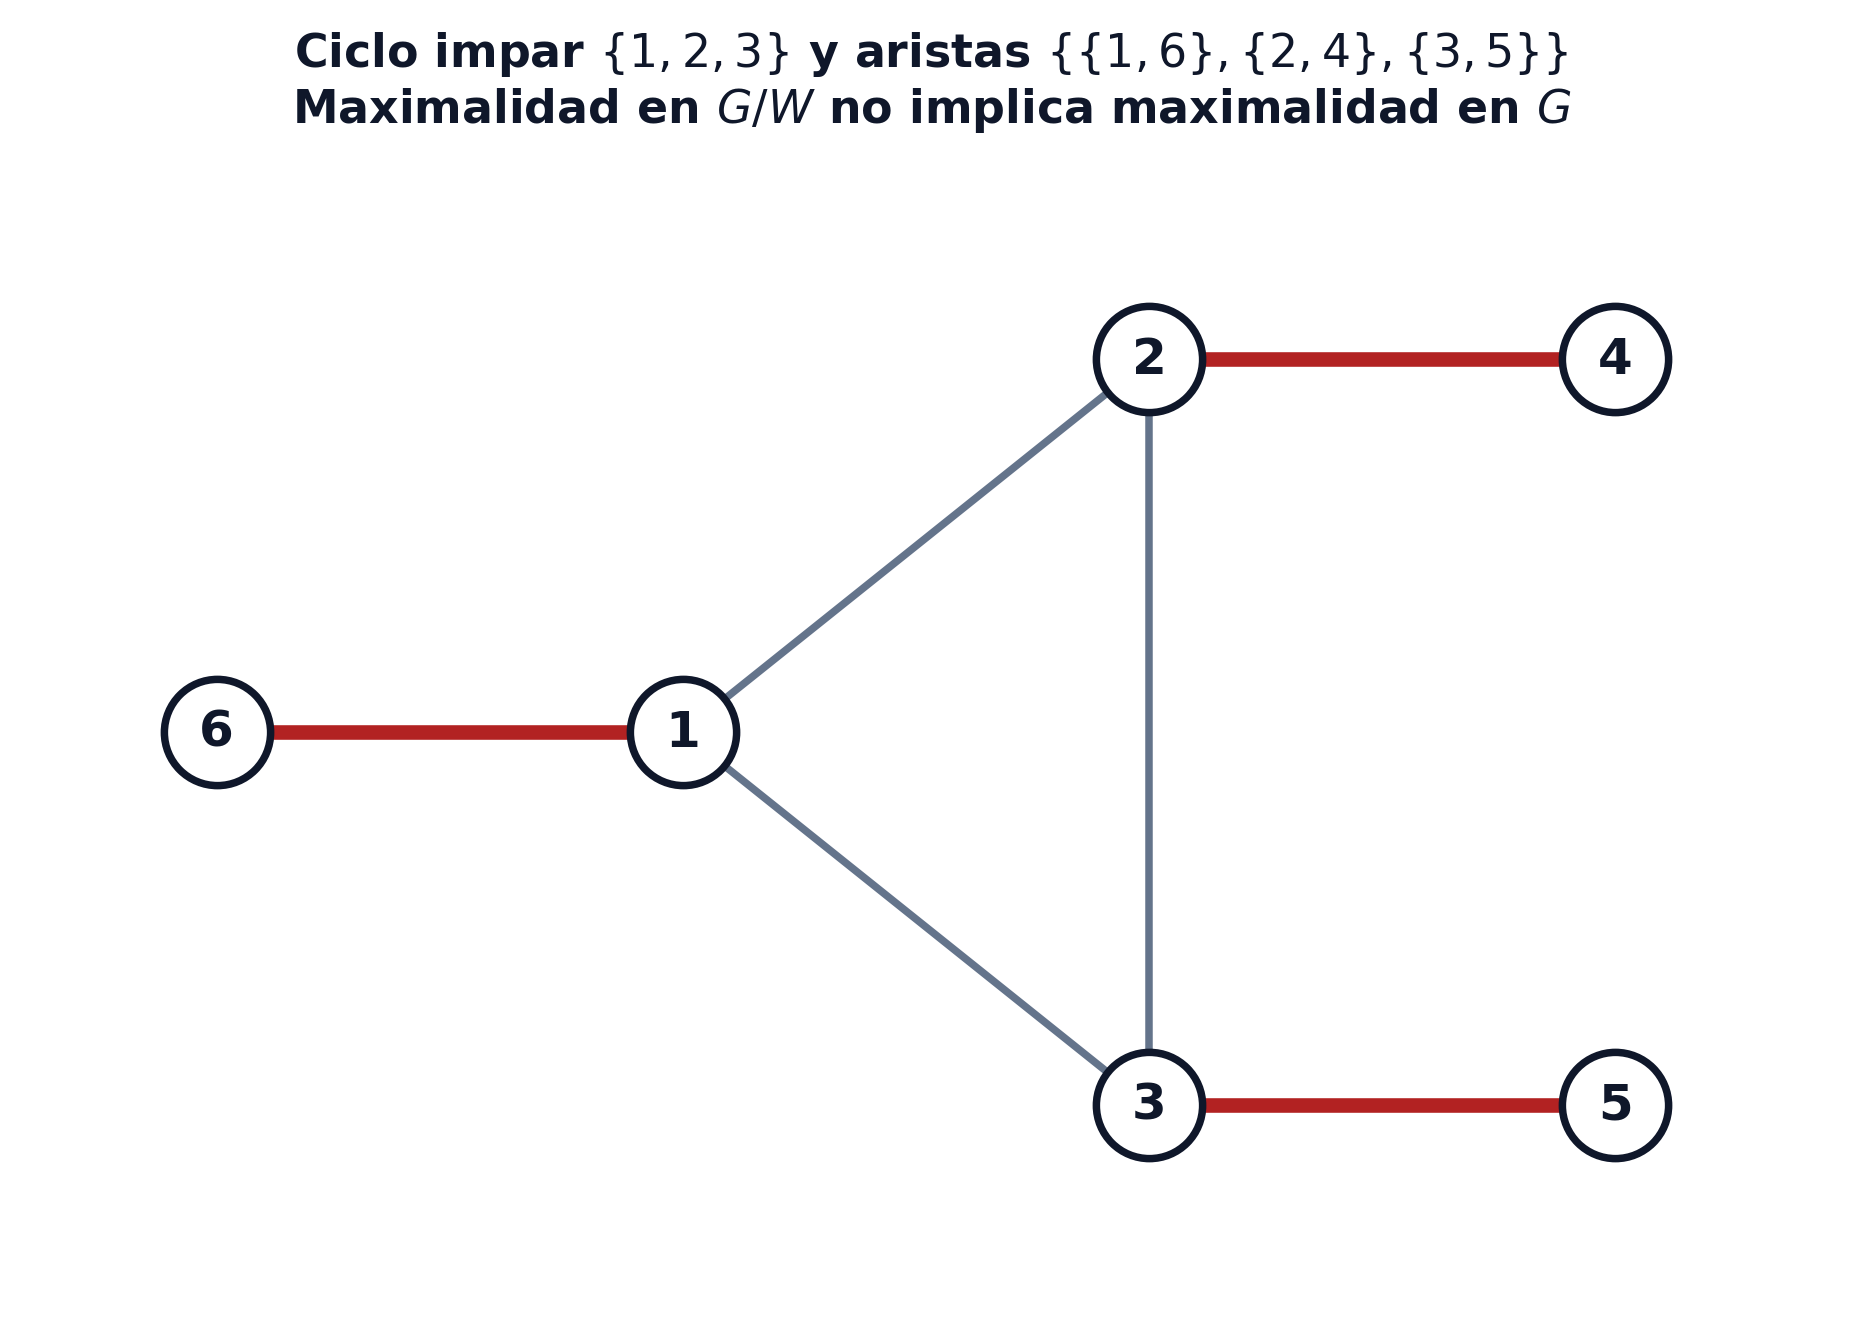
\includegraphics[width=0.65\linewidth,height=\textheight,keepaspectratio]{images/contraejemplo_maximalidad_contraccion.png}

}

\caption{\label{fig-contraejemplo-maximalidad}Contraejemplo de
maximalidad: grafo con ciclo impar \(\{1,2,3\}\) y emparejamiento óptimo
de cardinal 3}

\end{figure}%

\end{tcolorbox}

\subsection{Algoritmo de Flor de Edmonds: Esquema y resolución paso a
paso}\label{algoritmo-de-flor-de-edmonds-esquema-y-resoluciuxf3n-paso-a-paso}

Para aplicar y estructurar sistemáticamente el procedimiento de
exploración del árbol alternante en el \textbf{Paso C} del algoritmo de
Edmonds, se definen los siguientes elementos clave:

\begin{itemize}
\tightlist
\item
  \textbf{Árbol alternante \((Y, T)\)}: Subgrafo donde \(Y \subseteq V\)
  representa el conjunto de vértices explorados por el árbol y
  \(T \subseteq E\) el conjunto de aristas que forman la estructura del
  árbol.
\item
  \textbf{Conjunto de vértices pares (\(Y^0 \subset Y\))}: Vértices de
  \(Y\) conectados con la raíz del árbol (incluyendo a la propia raíz a
  distancia \(0\)) mediante una cadena alternante de longitud par.
\item
  \textbf{Propiedad estructural de las hojas}: Todas las hojas (extremos
  terminales) del árbol alternante deben ser obligatoriamente vértices
  pares (\(Y^0\)).
\end{itemize}

Como se ilustra en la Figura~\ref{fig-arbol-alternante-estructura},
considérese el árbol alternante con vértices
\(Y = \{0, 1, 2, 3, 4, 5, 6, 7, 8\}\), cuya raíz es el vértice expuesto
\(r = 0\). Los niveles se organizan alternadamente:

\begin{itemize}
\tightlist
\item
  \textbf{Nivel 0 (Raíz)}: Vértice \(0 \in Y^0\) (par, en rojo).
\item
  \textbf{Nivel 1 (Impar)}: Vértices \(\{1, 3\}\) (conectados por
  aristas fuera de \(K\)).
\item
  \textbf{Nivel 2 (Par)}: Vértices \(\{2, 4\} \subset Y^0\) (conectados
  por aristas dentro de \(K\), en rojo).
\item
  \textbf{Nivel 3 (Impar)}: Vértices \(\{5, 7\}\) (conectados por
  aristas fuera de \(K\)).
\item
  \textbf{Nivel 4 (Par)}: Vértices \(\{6, 8\} \subset Y^0\) (conectados
  por aristas dentro de \(K\), en rojo).
\end{itemize}

En este árbol, el conjunto de vértices pares es exactamente: \[
Y^0 = \{0, 2, 4, 6, 8\}
\]

\begin{figure}

\centering{

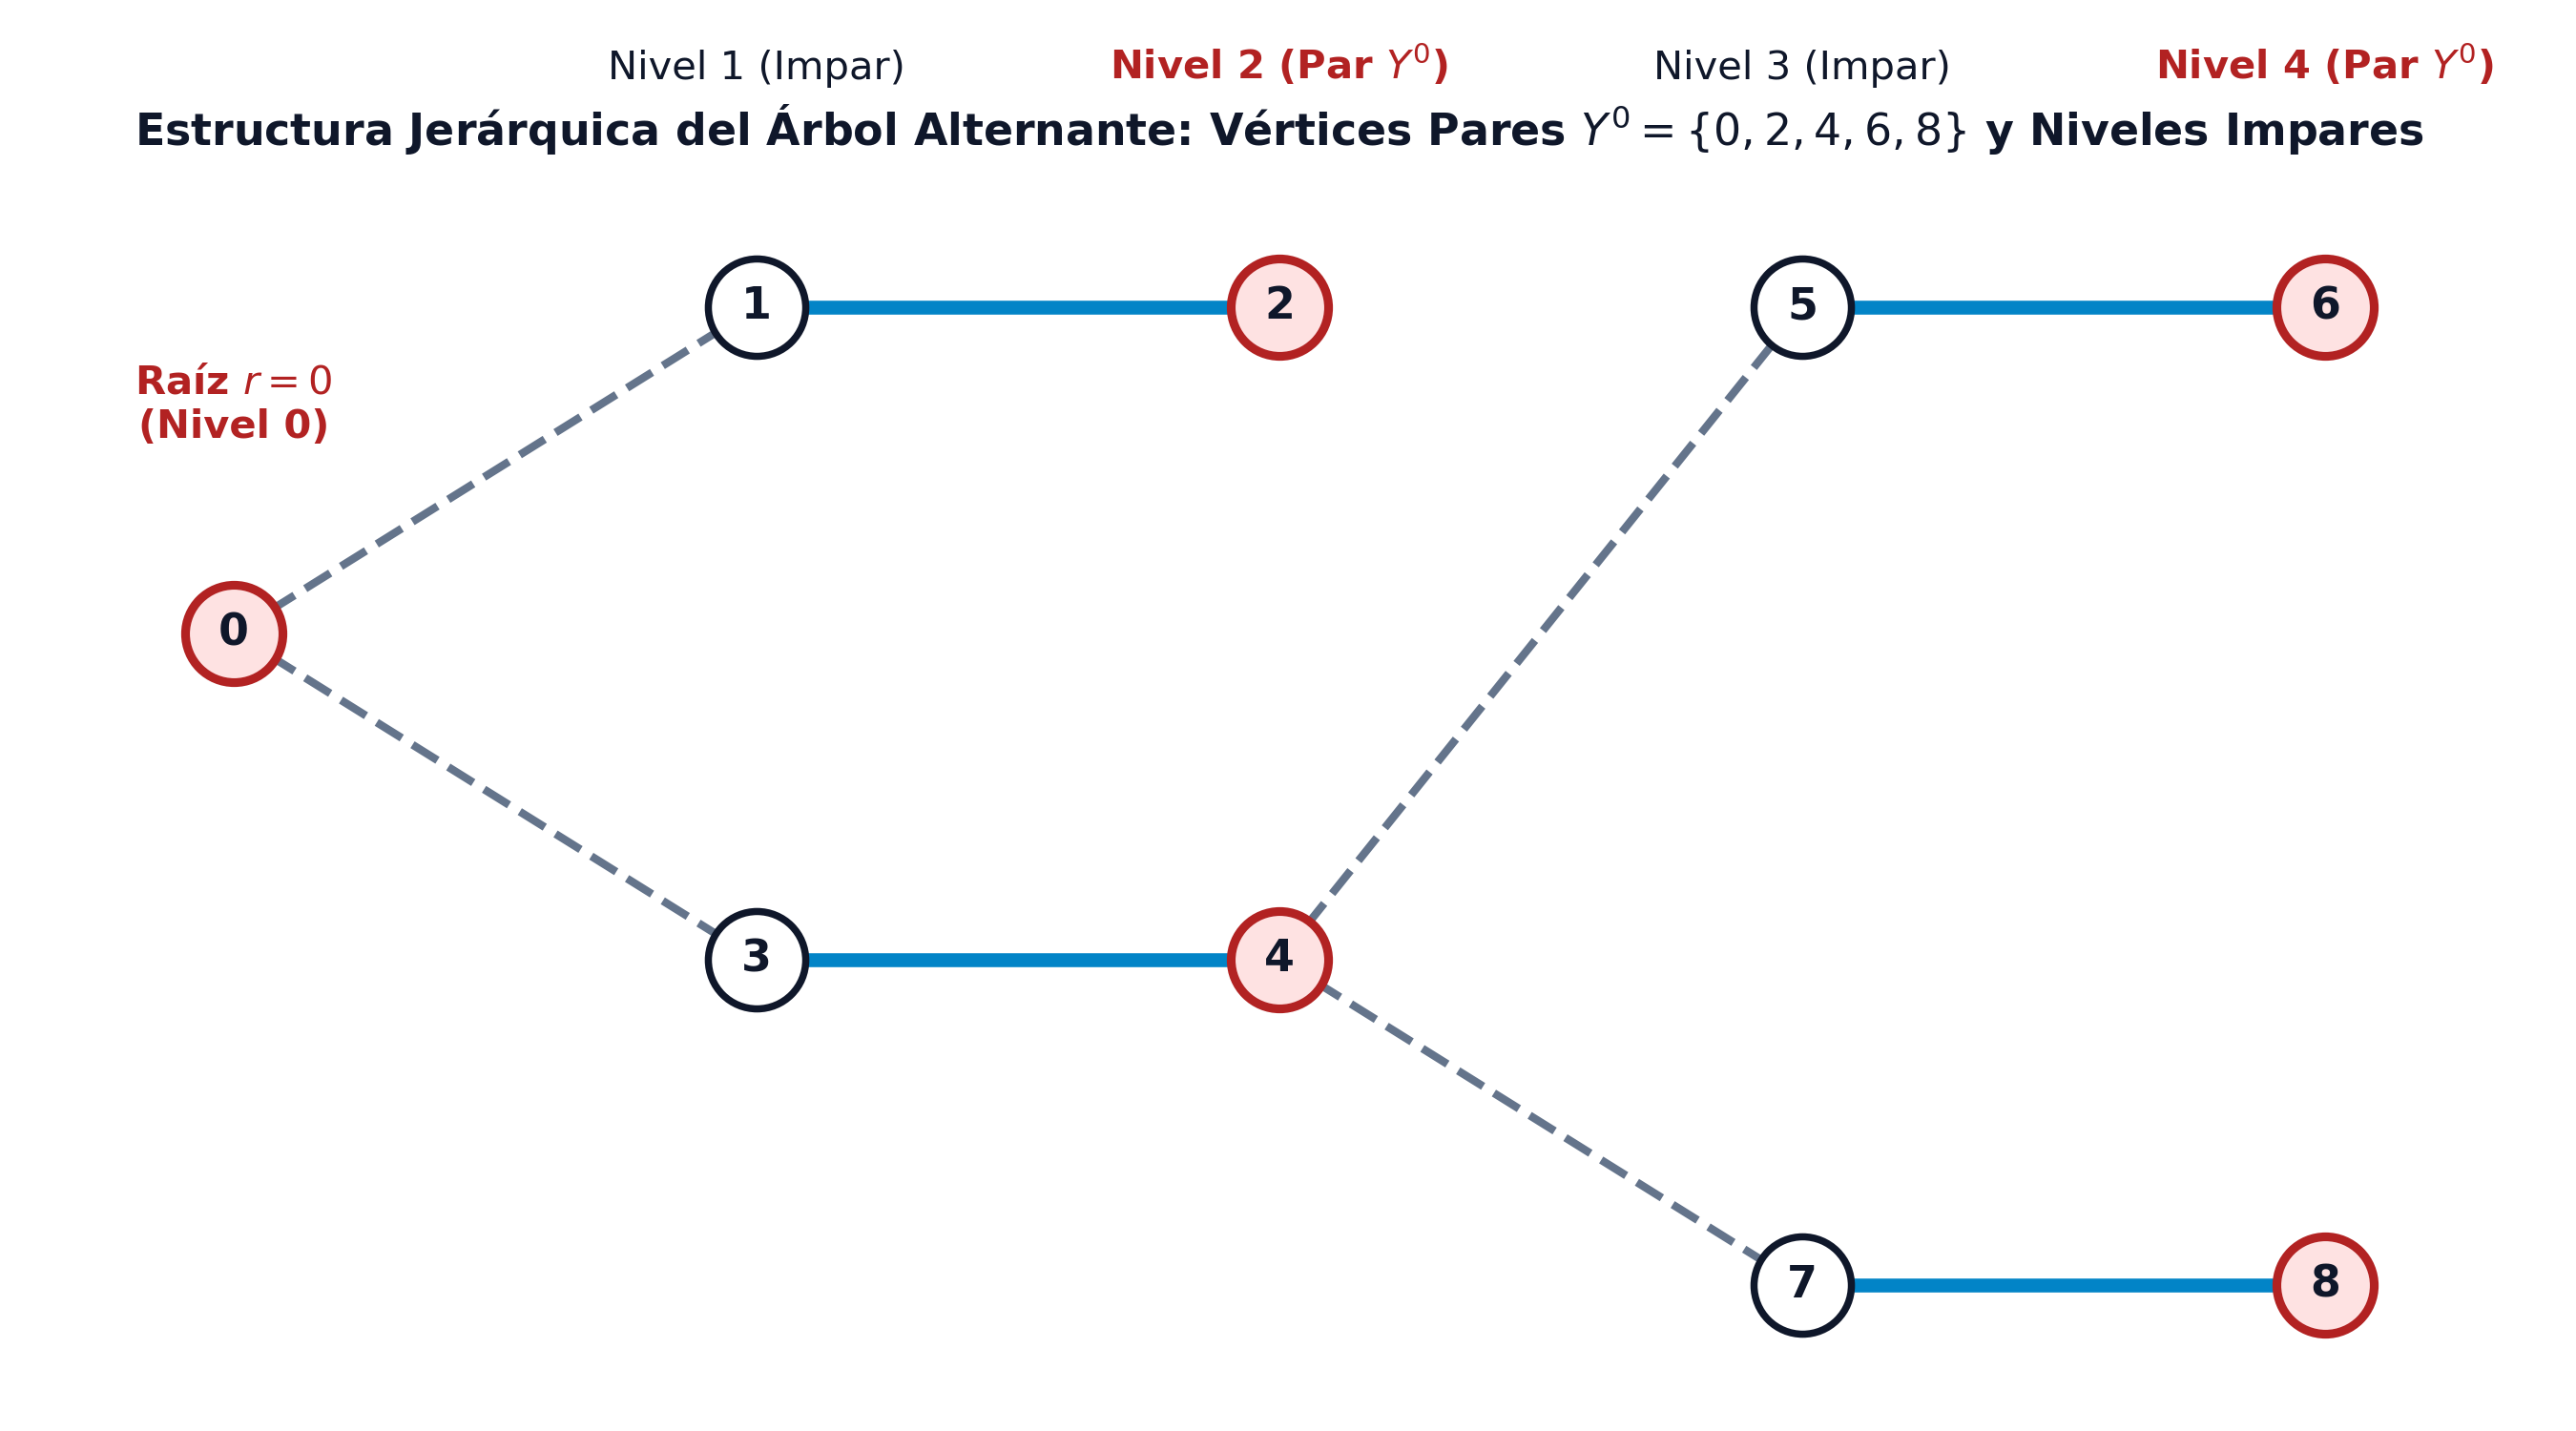
\includegraphics[width=0.85\linewidth,height=\textheight,keepaspectratio]{images/arbol_alternante_estructura.png}

}

\caption{\label{fig-arbol-alternante-estructura}Estructura jerárquica
del árbol alternante con \(Y=\{0,\dots,8\}\) destacando los vértices
pares \(Y^0 = \{0, 2, 4, 6, 8\}\) (en rojo) y los niveles impares}

\end{figure}%

A partir de los vértices pares \(Y^0\), la exploración del árbol
alternante se rige por las siguientes reglas operativas:

\begin{enumerate}
\def\labelenumi{\arabic{enumi}.}
\tightlist
\item
  \textbf{Detección de Ciclos Impares (Flores)}: Si en el grafo original
  existen dos vértices de \(Y^0\) conectados directamente por una arista
  \(\{i, j\} \in E\), se ha formado un \textbf{ciclo de longitud impar}
  (flor). Dicho ciclo debe contraerse en un supernodo \(w\) para
  continuar la búsqueda.
\item
  \textbf{Expansión del Árbol desde \(Y^0\)}: Si no se detectan ciclos
  impares entre nodos pares, se examinan las aristas incidentes en
  vértices de \(Y^0\) hacia nodos exteriores al árbol (\(j \notin Y\)):

  \begin{itemize}
  \tightlist
  \item
    \textbf{Hacia vértices adyacentes no saturados (\(sat(j) = 0\))}: Se
    detecta una \textbf{cadena alternante incremental} que une la raíz
    con \(j\), permitiendo aumentar de inmediato el cardinal del
    emparejamiento.
  \item
    \textbf{Hacia vértices adyacentes saturados (\(sat(j) = 1\))}: Si
    \(j\) está saturado por una arista \(\{j, k\} \in K\), se añade el
    par de aristas al árbol, incorporando el vértice \(k\) al conjunto
    de vértices pares \(Y^0\).
  \end{itemize}
\end{enumerate}

El algoritmo completo de Edmonds se sintetiza en el siguiente esquema
formal:

\begin{tcolorbox}[enhanced jigsaw, toprule=.15mm, opacitybacktitle=0.6, coltitle=black, colbacktitle=quarto-callout-note-color!10!white, title=\textcolor{quarto-callout-note-color}{\faInfo}\hspace{0.5em}{Esquema: Algoritmo de Flor de Edmonds para Emparejamiento Máximo}, arc=.35mm, rightrule=.15mm, toptitle=1mm, breakable, bottomtitle=1mm, titlerule=0mm, colback=white, opacityback=0, leftrule=.75mm, colframe=quarto-callout-note-color-frame, left=2mm, bottomrule=.15mm]

\begin{itemize}
\tightlist
\item
  \textbf{Paso A (Inicialización)}: Encontrar un emparejamiento inicial
  factible \(K\) en \(G\) (por ejemplo, el emparejamiento trivial
  \(K = \emptyset\)).
\item
  \textbf{Paso B (Condición de parada elemental)}: Si el número de
  vértices no saturados por \(K\) es \(0\) o \(1\), \textbf{PARAR}:
  \(K\) es de máximo cardinal. En caso contrario, ir al \textbf{Paso C}.
\item
  \textbf{Paso C (Construcción del Árbol Alternante)}:

  \begin{itemize}
  \tightlist
  \item
    \textbf{Paso C.1}: Seleccionar un vértice expuesto \(i_0 \in V\)
    (\(sat(i_0) = 0\)). Inicializar el árbol con \(Y = Y^0 = \{i_0\}\) y
    \(T = \emptyset\).
  \item
    \textbf{Paso C.2 (Exploración desde vértices pares \(Y^0\))}:

    \begin{itemize}
    \tightlist
    \item
      \textbf{Caso 1 (Detección de Flor / Ciclo Impar)}: Si existen dos
      vértices \(i, j \in Y^0\) tales que \(\{i, j\} \in E\), se detecta
      un ciclo impar. Contraer el ciclo definiendo el grafo comprimido
      \(G \leftarrow G/W\), actualizar el árbol
      (\(Y \leftarrow (Y \setminus W) \cup \{w\}\),
      \(Y^0 \leftarrow (Y^0 \setminus W) \cup \{w\}\)) y volver al
      \textbf{Paso C.2}.
    \item
      \textbf{Caso 2 (Extensión del Árbol)}: Si existe \(i \in Y^0\) y
      un vértice adyacente saturado \(j \notin Y\) con
      \(\{i, j\} \in E\) y \(\{j, k\} \in K\), añadir las aristas
      \(\{i, j\}\) y \(\{j, k\}\) al árbol:
      \(Y \leftarrow Y \cup \{j, k\}\),
      \(Y^0 \leftarrow Y^0 \cup \{k\}\),
      \(T \leftarrow T \cup \{\{i, j\}, \{j, k\}\}\) y volver al
      \textbf{Paso C.2}.
    \item
      \textbf{Caso 3 (Detección de Cadena Incremental)}: Si existe
      \(i \in Y^0\) y un vértice adyacente expuesto \(j \notin Y\)
      (\(sat(j) = 0\)) con \(\{i, j\} \in E\), se ha detectado una
      \textbf{cadena incremental} entre la raíz \(i_0\) y \(j\).
      Realizar la transferencia \(K \leftarrow K \bigtriangleup \mu\),
      descontraer todas las flores activas reconstruyendo el
      emparejamiento en el grafo original, y volver al \textbf{Paso B}.
    \item
      \textbf{Caso 4 (Árbol Bloqueado / Húngaro)}: Si no es posible
      aplicar ninguno de los casos anteriores desde los vértices de
      \(Y^0\), no existe ninguna cadena incremental conectada a \(i_0\).
      Fijar \(i_0\) como no aumentable. Si quedan otros vértices
      expuestos sin explorar, inicializar un nuevo árbol (Paso C.1); en
      caso contrario, \textbf{PARAR}: \(K\) es de \textbf{máximo
      cardinal}.
    \end{itemize}
  \end{itemize}
\end{itemize}

\end{tcolorbox}

\begin{tcolorbox}[enhanced jigsaw, toprule=.15mm, opacitybacktitle=0.6, coltitle=black, colbacktitle=quarto-callout-tip-color!10!white, title=\textcolor{quarto-callout-tip-color}{\faLightbulb}\hspace{0.5em}{Ejemplo: Traza completa del Algoritmo de Edmonds con contracciones
sucesivas}, arc=.35mm, rightrule=.15mm, toptitle=1mm, breakable, bottomtitle=1mm, titlerule=0mm, colback=white, opacityback=0, leftrule=.75mm, colframe=quarto-callout-tip-color-frame, left=2mm, bottomrule=.15mm]

Considérese el grafo de 8 vértices \(V = \{1, 2, 3, 4, 5, 6, 7, 8\}\)
ilustrado en la \textbf{?@fig-edmonds-animado}, cuyas aristas son: \[
\begin{aligned}
E = \bigl\{ & \{6,7\}, \, \{7,8\}, \, \{1,2\}, \, \{2,3\}, \, \{3,4\}, \\
& \{4,5\}, \, \{4,6\}, \, \{1,5\}, \, \{1,7\}, \, \{2,8\} \bigr\}
\end{aligned}
\]

A continuación se detalla la ejecución paso a paso del algoritmo desde
el emparejamiento nulo:

\begin{enumerate}
\def\labelenumi{\arabic{enumi}.}
\tightlist
\item
  \textbf{Fase Inicial}:

  \begin{itemize}
  \tightlist
  \item
    \textbf{Paso A (Inicialización)}: Comenzamos con el emparejamiento
    nulo \(K = \emptyset\). Conjunto de vértices expuestos (no
    saturados): \(\{1, 2, 3, 4, 5, 6, 7, 8\}\).
  \item
    \textbf{Paso B (Comprobación)}: Hay 8 vértices no saturados
    (\(> 1\)). No se cumple la condición de parada elemental
    \(\implies\) Ir al \textbf{Paso C}.
  \end{itemize}
\item
  \textbf{Iteración 1}:

  \begin{itemize}
  \tightlist
  \item
    \textbf{Paso C.1}: Seleccionamos la raíz expuesta \(i_0 = 1\). Se
    inicializa el árbol alternante: \(Y = Y^0 = \{1\}\),
    \(T = \emptyset\).
  \item
    \textbf{Paso C.2}:

    \begin{itemize}
    \tightlist
    \item
      \emph{Caso 1 (Ciclo impar)}: No hay ciclos impares en \(Y^0\).
    \item
      \emph{Caso 2 (Adyacente saturado)}: No existen vecinos saturados
      por \(K = \emptyset\).
    \item
      \emph{Caso 3 (Adyacente no saturado)}: Para \(i = 1 \in Y^0\),
      existe el vértice adyacente expuesto \(j = 2 \notin Y\) con
      \(\{1,2\} \in E\). Se detecta la cadena incremental elemental
      \(\mu = (1, 2)\).
    \item
      \emph{Transferencia}: Realizamos
      \(K \leftarrow K \bigtriangleup \{\{1,2\}\} = \bigl\{ \{1,2\} \bigr\}\).
    \item
      \textbf{Volver al Paso B}.
    \end{itemize}
  \end{itemize}
\item
  \textbf{Iteración 2}:

  \begin{itemize}
  \item
    \textbf{Paso B (Comprobación)}: Con \(K = \bigl\{ \{1,2\} \bigr\}\),
    quedan 6 vértices no saturados \(\{3, 4, 5, 6, 7, 8\} > 1 \implies\)
    Ir al \textbf{Paso C}.
  \item
    \textbf{Paso C.1}: Seleccionamos la raíz expuesta \(i_0 = 3\). Se
    inicializa el árbol alternante: \(Y = Y^0 = \{3\}\),
    \(T = \emptyset\).
  \item
    \textbf{Paso C.2 (Extensión)}: Para \(3 \in Y^0\), existe el vecino
    saturado \(2 \notin Y\) (saturado por \(\{1,2\} \in K\)) con
    \(\{2,3\} \in E\). Aplicando el Caso 2, incorporamos las aristas
    \(\{2,3\}\) y \(\{1,2\}\) al árbol:
    \[Y = \{1, 2, 3\}, \quad Y^0 = \{1, 3\}, \quad T = \bigl\{ \{2,3\}, \, \{1,2\} \bigr\}\]
    Volvemos a evaluar el \textbf{Paso C.2}.
  \item
    \textbf{Paso C.2 (Detección de Cadena Incremental)}: Evaluando desde
    los vértices pares \(Y^0 = \{1, 3\}\), para \(3 \in Y^0\) existe el
    vecino expuesto \(4 \notin Y\) con \(\{3,4\} \in E\) (Caso 3). Se
    detecta la cadena incremental \(\mu = (3, 4)\).
  \item
    \textbf{Transferencia}: Realizamos
    \(K \leftarrow K \bigtriangleup \{\{3,4\}\} = \bigl\{ \{1,2\}, \, \{3,4\} \bigr\}\).
  \item
    \textbf{Volver al Paso B}.
  \end{itemize}
\item
  \textbf{Iteración 3 (Detección y Contracción de la Primera Flor
  \(W\))}:

  \begin{itemize}
  \item
    \textbf{Paso B (Comprobación)}: Con
    \(K = \bigl\{ \{1,2\}, \{3,4\} \bigr\}\), quedan 4 vértices
    expuestos \(\{5, 6, 7, 8\} > 1 \implies\) Ir al \textbf{Paso C}.
  \item
    \textbf{Paso C.1}: Seleccionamos la raíz expuesta \(i_0 = 5\).
    Inicializamos el árbol alternante: \(Y = Y^0 = \{5\}\),
    \(T = \emptyset\).
  \item
    \textbf{Paso C.2 (Extensión 1)}: Para \(5 \in Y^0\), existe el
    vecino saturado \(1 \notin Y\) (saturado por \(\{1,2\} \in K\)).
    Aplicando el Caso 2, incorporamos las aristas \(\{5,1\}\) y
    \(\{1,2\}\) al árbol:
    \[Y = \{1, 2, 5\}, \quad Y^0 = \{2, 5\}, \quad T = \bigl\{ \{5,1\}, \, \{1,2\} \bigr\}\]
    Volvemos al \textbf{Paso C.2}.
  \item
    \textbf{Paso C.2 (Extensión 2)}: Para \(5 \in Y^0\), existe el
    vecino saturado \(4 \notin Y\) (saturado por \(\{3,4\} \in K\)).
    Aplicando el Caso 2, incorporamos las aristas \(\{5,4\}\) y
    \(\{4,3\}\) al árbol:
    \[Y = \{1, 2, 3, 4, 5\}, \quad Y^0 = \{2, 3, 5\}, \quad T = \bigl\{ \{5,1\}, \, \{1,2\}, \, \{5,4\}, \, \{4,3\} \bigr\}\]
    Volvemos al \textbf{Paso C.2}.
  \item
    \textbf{Paso C.2 (Caso 1: Detección de Flor)}: Entre los nodos pares
    del árbol \(Y^0 = \{2, 3, 5\}\), existe la arista
    \(\{2, 3\} \in E\). Al conectar dos vértices de la misma paridad
    respecto a la raíz, se identifica el ciclo impar (flor) de 5
    vértices: \[W = \{1, 2, 3, 4, 5\}\]
  \item
    \textbf{Contracción de la Flor \(W\)}: Comprimimos todo el
    subconjunto \(W\) en el pseudonodo (supernodo) \(w\). Se define el
    grafo comprimido \(G/W\) con vértices \(\{w, 6, 7, 8\}\) y aristas
    \(\{ \{w,6\}, \{w,7\}, \{w,8\}, \{6,7\}, \{7,8\} \}\). En \(G/W\),
    el árbol se actualiza a \(Y = Y^0 = \{w\}\), \(T = \emptyset\) y
    \(K = \emptyset\).
  \item
    \textbf{Paso C.2 en \(G/W\) (Transferencia)}: Desde \(w \in Y^0\),
    se explora la arista \(\{w,6\}\) hacia el vértice expuesto
    \(6 \notin Y\) (Caso 3). Se realiza la transferencia en \(G/W\):
    \[K = \bigl\{ \{w, 6\} \bigr\}\] \textbf{Volver al Paso B}.
  \end{itemize}
\item
  \textbf{Iteración 4 (Búsqueda en \(G/W\) y Contracción de la Segunda
  Flor \(W'\))}:

  \begin{itemize}
  \item
    \textbf{Paso B (Comprobación en \(G/W\))}: Con
    \(K = \bigl\{ \{w, 6\} \bigr\}\), los vértices no saturados en
    \(G/W\) son \(\{7, 8\}\) (\(2 > 1\)) \(\implies\) Ir al \textbf{Paso
    C}.
  \item
    \textbf{Paso C.1}: Seleccionamos la raíz expuesta \(i_0 = 7\).
    Inicializamos el árbol: \(Y = Y^0 = \{7\}\), \(T = \emptyset\).
  \item
    \textbf{Paso C.2 (Extensión)}: Para \(7 \in Y^0\), el vecino
    \(w \notin Y\) está saturado por \(\{w, 6\} \in K\). Por Caso 2,
    añadimos \(\{7,w\}\) y \(\{w,6\}\) al árbol:
    \[Y = \{w, 6, 7\}, \quad Y^0 = \{6, 7\}, \quad T = \bigl\{ \{7,w\}, \, \{w,6\} \bigr\}\]
    Volvemos al \textbf{Paso C.2}.
  \item
    \textbf{Paso C.2 (Caso 1: Detección de Segunda Flor)}: Entre los
    nodos pares \(Y^0 = \{6, 7\}\), existe la arista \(\{6, 7\} \in E\).
    Se detecta el segundo ciclo impar: \[W' = \{w, 6, 7\}\]
  \item
    \textbf{Segunda Contracción}: Comprimimos \(W'\) en el pseudonodo
    \(w'\). Obtenemos el grafo comprimido \(G/W'\) con vértices
    \(\{w', 8\}\) y la arista \(\{w', 8\}\).
  \item
    \textbf{Paso C.2 en \(G/W'\) (Transferencia)}: La arista
    \(\{w', 8\}\) une los dos únicos vértices (ambos expuestos) en
    \(G/W'\) (Caso 3). Transferencia: \(K = \bigl\{ \{w', 8\} \bigr\}\).
  \item
    \textbf{Paso B (Parada)}: En \(G/W'\), todos los vértices están
    saturados (quedan \(0\) vértices expuestos \(\le 1\)).
    \textbf{PARAR}: Se alcanza la optimalidad global.
  \end{itemize}
\item
  \textbf{Fase de Descompresión y Reconstrucción Óptima}:

  \begin{itemize}
  \item
    \textbf{Descompresión de \(W'\)}: Al descontraer el supernodo
    \(w'\), la arista \(\{w', 8\}\) proviene originalmente de
    \(\{7, 8\} \in E\). En el ciclo impar \(W' = \{w, 6, 7\}\), el nodo
    \(7\) queda saturado hacia el exterior por \(\{7, 8\}\), lo que deja
    en \(W'\) la arista \(\{w, 6\}\) para saturar a los nodos restantes.
    Obtenemos en \(G/W\): \[K = \bigl\{ \{w, 6\}, \, \{7, 8\} \bigr\}\]
  \item
    \textbf{Descompresión de \(W\)}: La arista \(\{w, 6\}\) proviene
    originalmente de la arista exterior \(\{4, 6\} \in E\). En la flor
    \(W = \{1, 2, 3, 4, 5\}\), el vértice \(4\) queda saturado hacia el
    exterior por \(\{4, 6\}\). Seleccionamos en \(W\) el emparejamiento
    que satura a los 4 vértices restantes \(\{1, 2, 3, 5\}\),
    correspondiente a \(\{1, 5\}\) y \(\{2, 3\}\).
  \item
    \textbf{Emparejamiento Óptimo Final}: Reconstruyendo todas las
    aristas en el grafo original \(G\), obtenemos: \[
    K^* = \bigl\{ \{1, 5\}, \, \{2, 3\}, \, \{4, 6\}, \, \{7, 8\} \bigr\}
    \] El cardinal resultante es \(|K^*| = 4 = 8/2\), alcanzando un
    \textbf{emparejamiento perfecto} en el grafo de 8 nodos.
  \end{itemize}
\end{enumerate}

\end{tcolorbox}

\section{Problemas de recubrimiento en grafos y relaciones de
dualidad}\label{problemas-de-recubrimiento-en-grafos-y-relaciones-de-dualidad}

Existe una estrecha relación de complementariedad y dualidad entre
seleccionar conjuntos de aristas independientes (emparejamientos) y
seleccionar conjuntos de aristas que cubran todos los vértices de una
red. Para introducir este concepto, consideremos el problema de diseño
de patrullas de vigilancia en recintos fortificados.

\begin{tcolorbox}[enhanced jigsaw, toprule=.15mm, opacitybacktitle=0.6, coltitle=black, colbacktitle=quarto-callout-tip-color!10!white, title=\textcolor{quarto-callout-tip-color}{\faLightbulb}\hspace{0.5em}{Ejemplo: Vigilancia de murallas en la fortaleza}, arc=.35mm, rightrule=.15mm, toptitle=1mm, breakable, bottomtitle=1mm, titlerule=0mm, colback=white, opacityback=0, leftrule=.75mm, colframe=quarto-callout-tip-color-frame, left=2mm, bottomrule=.15mm]

Considérese el recinto fortificado de \(12\) torres de vigilancia
conectadas mediante \(12\) tramos de muralla, representado en la
Figura~\ref{fig-recubrimiento-aristas-fortaleza}.

Se desea posicionar patrullas de centinelas sobre las murallas. Cada
guardia asignado a una muralla \(\{u, v\}\) vigila simultáneamente las
dos torres situadas en sus extremos (\(u\) y \(v\)). El objetivo
consiste en \textbf{determinar el número mínimo de guardias (murallas)}
necesarios para que \textbf{todas las torres de la fortaleza queden
vigiladas}.

\begin{figure}[H]

\centering{

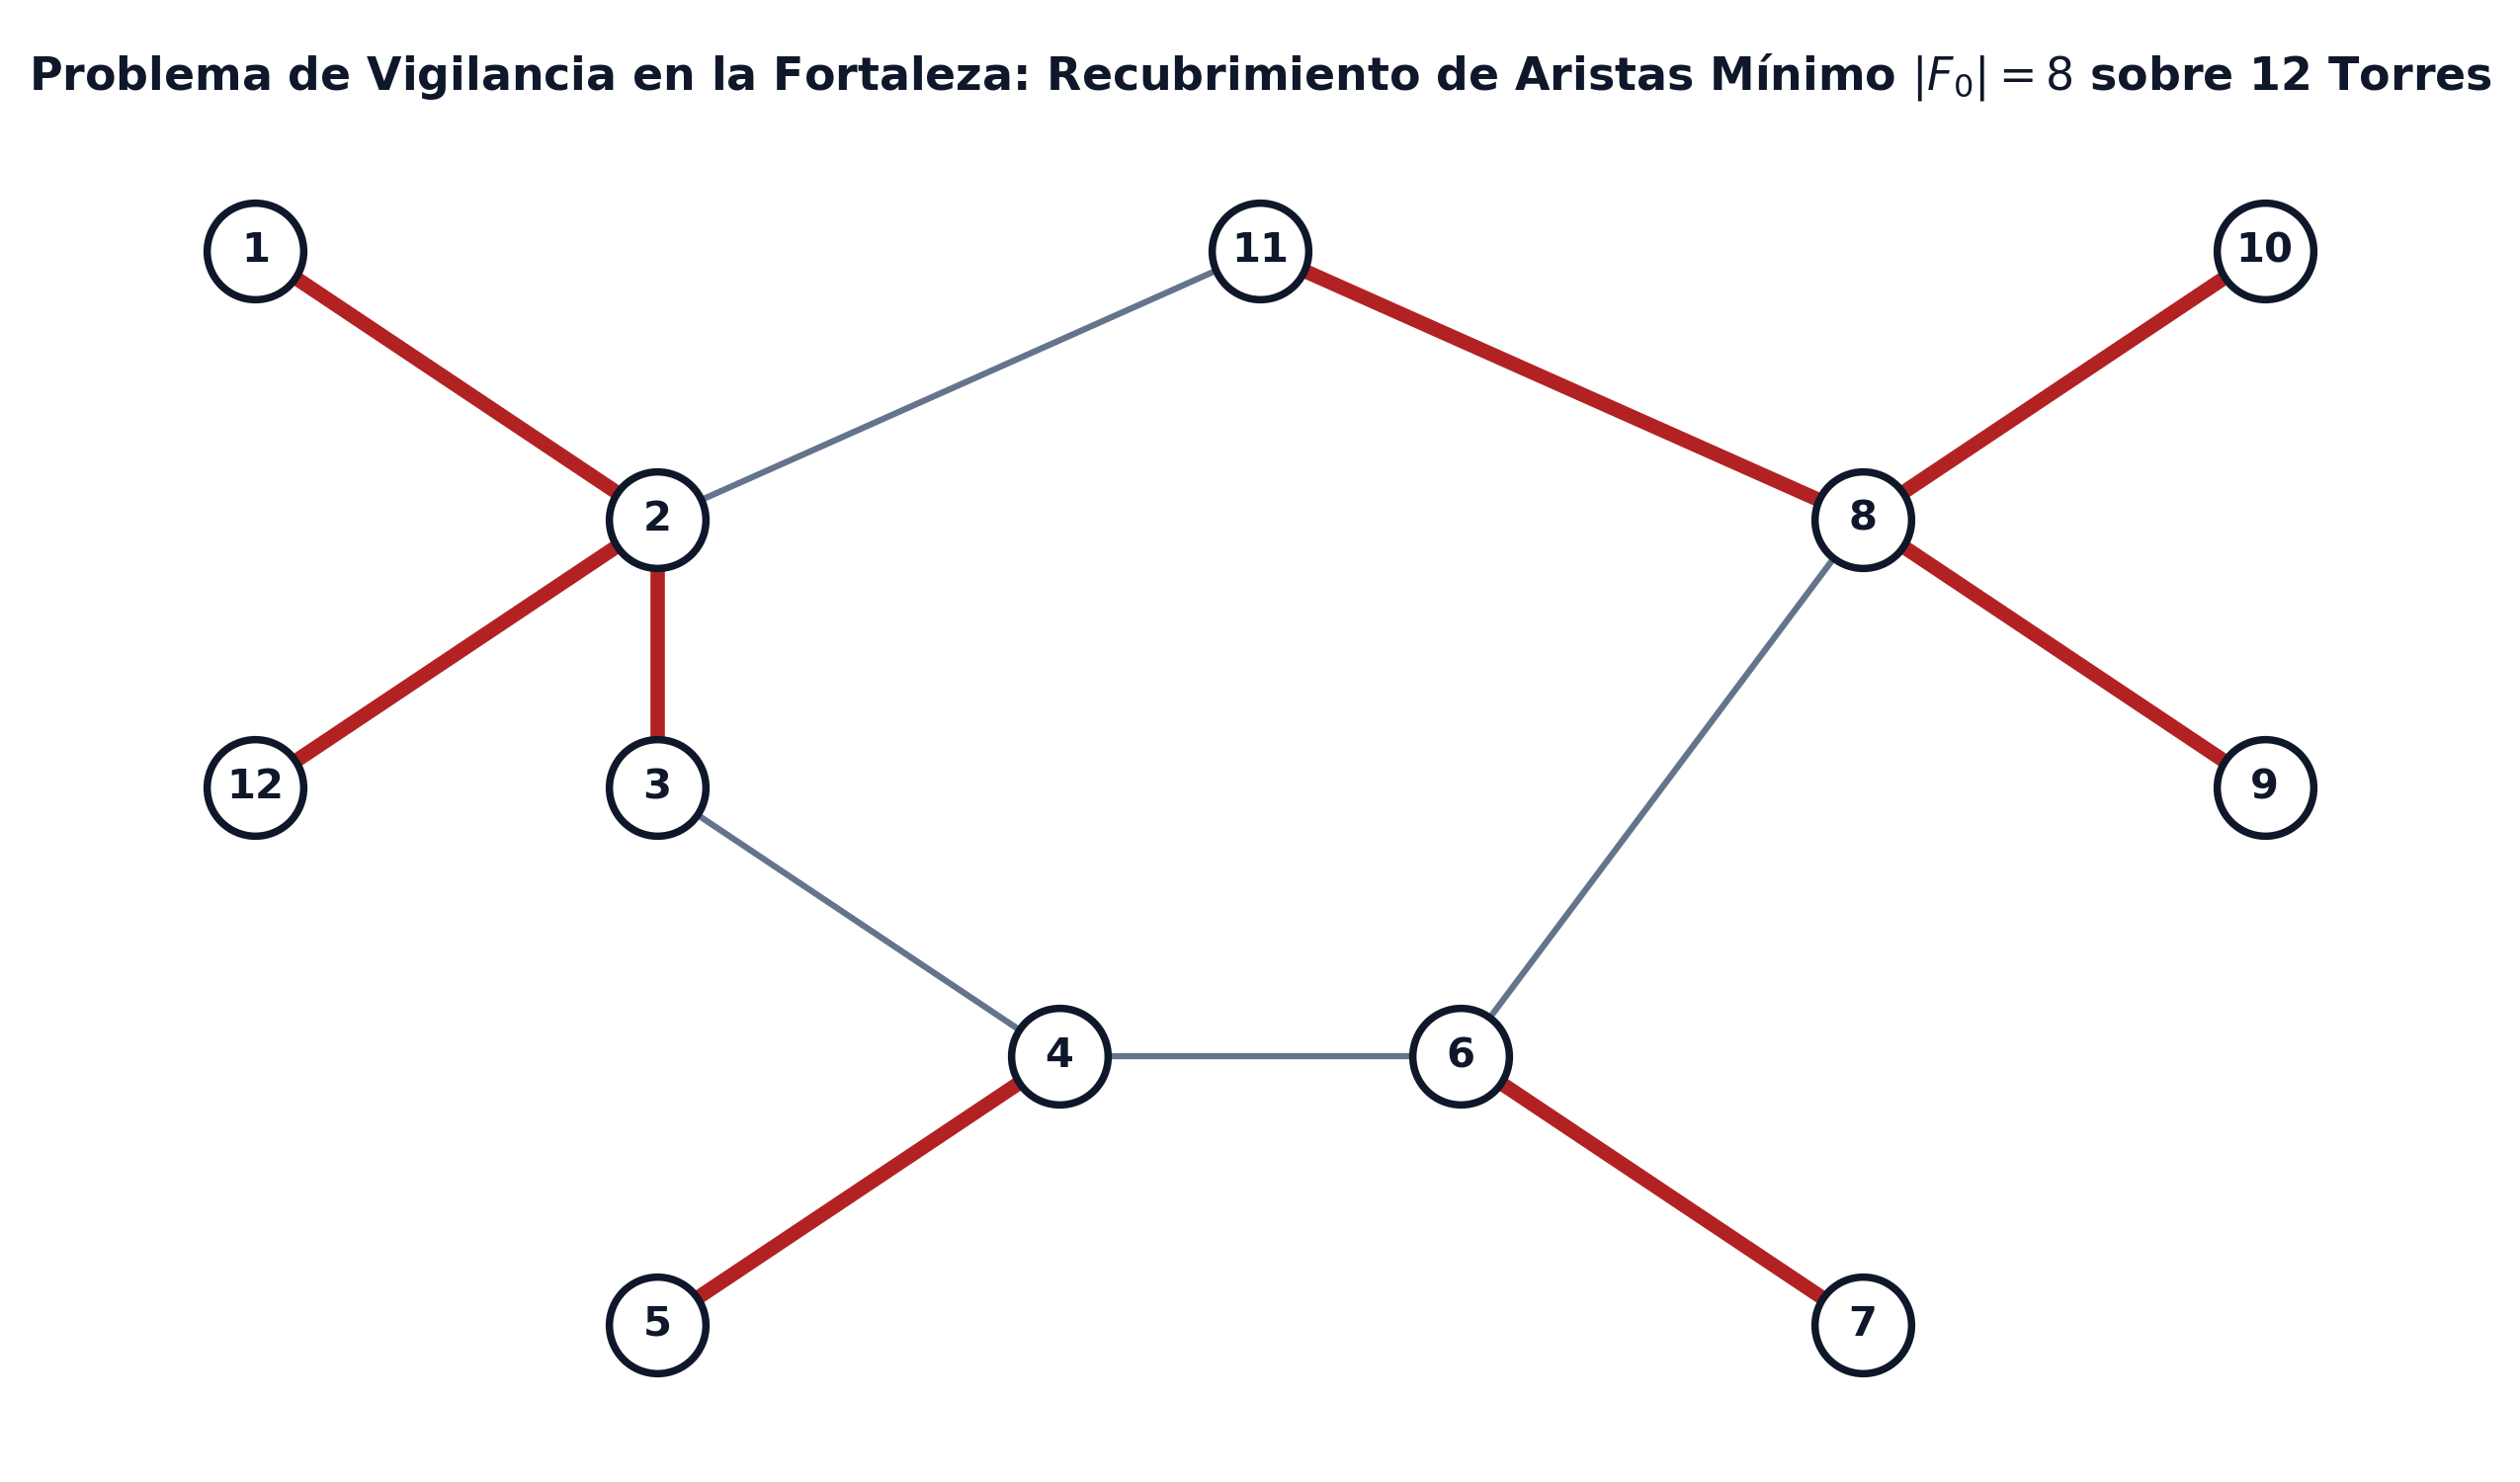
\includegraphics[width=0.75\linewidth,height=\textheight,keepaspectratio]{images/recubrimiento_aristas_fortaleza.png}

}

\caption{\label{fig-recubrimiento-aristas-fortaleza}Problema de
vigilancia en la fortaleza: recubrimiento de aristas mínimo
\(|F_0| = 8\) sobre 12 torres}

\end{figure}%

Modelando la fortaleza como un grafo \(G = (V, E)\), el problema
consiste en hallar un subconjunto de aristas \(F \subseteq E\) de mínimo
cardinal tal que todo vértice \(v \in V\) sea incidente en al menos una
arista de \(F\). Como se observa en la figura, seleccionando las 8
aristas en rojo: \[
F_0 = \bigl\{ \{1,2\}, \, \{2,12\}, \, \{2,3\}, \, \{4,5\}, \, \{6,7\}, \, \{8,9\}, \, \{8,10\}, \, \{8,11\} \bigr\}
\] se cubren las 12 torres con \(|F_0| = 8\) guardias, garantizando la
seguridad completa a coste mínimo.

\end{tcolorbox}

A partir del problema de la fortaleza, se formaliza la noción de
subconjunto de aristas que cubre la totalidad de los vértices del grafo.
A diferencia del problema de emparejamiento (donde se busca que cada
nodo esté saturado a lo sumo una vez por las aristas seleccionadas,
\(\sum x_e \le 1\)), en el problema de recubrimiento se exige que todo
nodo esté cubierto al menos una vez (\(\sum x_e \ge 1\)).

\begin{tcolorbox}[enhanced jigsaw, toprule=.15mm, opacitybacktitle=0.6, coltitle=black, colbacktitle=quarto-callout-note-color!10!white, title=\textcolor{quarto-callout-note-color}{\faInfo}\hspace{0.5em}{Definición: Recubrimiento de aristas (Edge Cover)}, arc=.35mm, rightrule=.15mm, toptitle=1mm, breakable, bottomtitle=1mm, titlerule=0mm, colback=white, opacityback=0, leftrule=.75mm, colframe=quarto-callout-note-color-frame, left=2mm, bottomrule=.15mm]

Dado un grafo no dirigido \(G = (V, E)\) sin vértices aislados, un
\textbf{recubrimiento de aristas} (o \emph{edge cover}) es un
subconjunto de aristas \(F \subseteq E\) tal que todo vértice
\(v \in V\) es incidente en al menos una arista de \(F\), es decir:

\[
\bigcup_{e \in F} e = V
\]

\end{tcolorbox}

\begin{tcolorbox}[enhanced jigsaw, toprule=.15mm, opacitybacktitle=0.6, coltitle=black, colbacktitle=quarto-callout-note-color!10!white, title=\textcolor{quarto-callout-note-color}{\faInfo}\hspace{0.5em}{Proposición: Monotonía del recubrimiento}, arc=.35mm, rightrule=.15mm, toptitle=1mm, breakable, bottomtitle=1mm, titlerule=0mm, colback=white, opacityback=0, leftrule=.75mm, colframe=quarto-callout-note-color-frame, left=2mm, bottomrule=.15mm]

Dado un grafo \(G = (V, E)\) y un recubrimiento de aristas
\(F \subseteq E\), si \(F' \subseteq E\) satisface \(F \subseteq F'\),
entonces \(F'\) es también un recubrimiento de aristas de \(G\).

\emph{Demostración}: Si cada vértice \(v \in V\) es incidente en alguna
arista de \(F\), la adición de aristas adicionales en \(F'\) preserva de
forma trivial la cobertura de todos los vértices. \(\blacksquare\)

\end{tcolorbox}

\subsection{Teorema fundamental de dualidad de
Gallai}\label{teorema-fundamental-de-dualidad-de-gallai}

La conexión cuantitativa exacta entre el emparejamiento de máximo
cardinal y el recubrimiento de mínimo cardinal fue establecida por Tibor
Gallai en 1959 (Gallai 1959).

\begin{tcolorbox}[enhanced jigsaw, toprule=.15mm, opacitybacktitle=0.6, coltitle=black, colbacktitle=quarto-callout-important-color!10!white, title=\textcolor{quarto-callout-important-color}{\faExclamation}\hspace{0.5em}{Teorema: Dualidad de Gallai para emparejamientos y recubrimientos}, arc=.35mm, rightrule=.15mm, toptitle=1mm, breakable, bottomtitle=1mm, titlerule=0mm, colback=white, opacityback=0, leftrule=.75mm, colframe=quarto-callout-important-color-frame, left=2mm, bottomrule=.15mm]

Sea \(G = (V, E)\) un grafo simple conexo con \(n = |V|\) vértices y sin
nodos aislados. Sean \(K_0 \subseteq E\) un emparejamiento de
\textbf{máximo cardinal} y \(F_0 \subseteq E\) un recubrimiento de
aristas de \textbf{mínimo cardinal}. Entonces se verifican las
siguientes propiedades:

\begin{enumerate}
\def\labelenumi{\arabic{enumi}.}
\item
  \textbf{Conservación de la Cardinalidad}: \[
  |K_0| + |F_0| = n
  \]
\item
  \textbf{Construcción del Recubrimiento Mínimo a partir de \(K_0\)}: El
  conjunto \(F_1\) obtenido añadiendo a \(K_0\) exactamente una arista
  incidente en cada uno de los \(n - 2|K_0|\) vértices expuestos por
  \(K_0\): \[
  F_1 = K_0 \cup \bigl\{ e_v \in E \mid v \in V \setminus V(K_0) \bigr\}
  \] es un \textbf{recubrimiento de aristas de mínimo cardinal}
  (\(|F_1| = |F_0|\)).
\item
  \textbf{Construcción del Emparejamiento Máximo a partir de \(F_0\)}:
  El conjunto \(K_1\) obtenido eliminando de \(F_0\) todas las aristas
  redundantes salvo una en cada vértice cubierto más de una vez
  (\(d_{F_0}(v) > 1\)): \[
  K_1 = F_0 \setminus \bigl\{ \text{aristas sobrantes en vértices de grado } > 1 \text{ en } F_0 \bigr\}
  \] es un \textbf{emparejamiento de máximo cardinal}
  (\(|K_1| = |K_0|\)).
\end{enumerate}

\emph{Demostración}: Demostramos constructivamente las tres afirmaciones
del teorema:

\begin{itemize}
\item
  \textbf{Parte 2 (Construcción de \(F_1\) y acotación superior)}: Sea
  \(K_0\) un emparejamiento de máximo cardinal. \(K_0\) satura
  exactamente a \(2|K_0|\) vértices, dejando \(n - 2|K_0|\) vértices
  expuestos. Como \(G\) no tiene vértices aislados, para cada vértice
  expuesto \(v \in V \setminus V(K_0)\) existe al menos una arista
  \(e_v \in E\) incidente en \(v\). Añadiendo una arista por cada
  vértice libre, el conjunto \(F_1\) cubre a todos los vértices de
  \(G\), constituyendo un recubrimiento válido. El número de aristas de
  \(F_1\) es exactamente: \[
  |F_1| = |K_0| + (n - 2|K_0|) = n - |K_0| \implies |F_1| + |K_0| = n
  \] Dado que \(F_0\) es el recubrimiento de mínimo cardinal, por
  definición \(|F_0| \le |F_1|\), luego: \[
  |F_0| + |K_0| \le n
  \]
\item
  \textbf{Parte 3 (Construcción de \(K_1\) y acotación inferior)}: Sea
  \(F_0\) un recubrimiento de aristas de mínimo cardinal. En \(F_0\), no
  pueden existir ciclos cerrados (eliminar una arista de un ciclo
  preservaría la cobertura de todos sus nodos, contradiciendo la
  minimalidad de \(F_0\)), ni cadenas de longitud mayor o igual a \(3\)
  (eliminar una arista interior mantendría cubiertos los extremos). Por
  tanto, el subgrafo \((V, F_0)\) está formado exclusivamente por
  estrellas conexas (árboles de profundidad 1) de aristas incidentes en
  centros comunes.

  Para cada componente estrella con \(k \ge 2\) aristas incidentes en un
  centro, eliminamos \(k - 1\) aristas, conservando una única arista por
  componente. El conjunto resultante \(K_1 \subset F_0\) no tiene
  aristas adyacentes, luego \(K_1\) es un emparejamiento válido de
  \(G\). Cada arista eliminada de \(F_0\) deja de saturar a exactamente
  un vértice hoja, por lo que el número de vértices no saturados por
  \(K_1\) es igual al número de aristas eliminadas:
  \(|F_0| - |K_1| = n - 2|K_1|\). Despejando: \[
  |K_1| = |F_0| - (n - 2|K_1|) \implies |F_0| + |K_1| = n
  \] Como \(K_0\) es el emparejamiento de máximo cardinal,
  \(|K_1| \le |K_0|\), por lo que: \[
  n = |F_0| + |K_1| \le |F_0| + |K_0|
  \]
\item
  \textbf{Conclusión de igualdad}: Combinando ambas desigualdades: \[
  n = |F_1| + |K_0| \ge |F_0| + |K_0| \ge |F_0| + |K_1| = n
  \] Todas las desigualdades intermedias deben cumplirse como igualdades
  estrictas: \[
  |F_1| = |F_0|, \quad |K_1| = |K_0|, \quad \text{y} \quad |K_0| + |F_0| = n
  \] Esto demuestra simultáneamente que \(|K_0| + |F_0| = n\), que
  \(F_1\) es un recubrimiento mínimo y que \(K_1\) es un emparejamiento
  máximo. \(\blacksquare\)
\end{itemize}

\end{tcolorbox}

El Teorema de Gallai establece una de las relaciones de conservación
combinatoria más profundas entre problemas de \textbf{empaquetamiento}
(\emph{packing}) y problemas de \textbf{recubrimiento}
(\emph{covering}). En cualquier grafo sin vértices aislados, cada arista
de un emparejamiento satura exactamente \(2\) vértices distintos,
mientras que cada arista adicional necesaria para completar un
recubrimiento cubre exactamente a \(1\) vértice libre. La identidad
\(|K_0| + |F_0| = n\) actúa como una ecuación de conservación
estructural: el déficit de aristas en el emparejamiento respecto del
total de nodos se traduce exactamente en el superávit de aristas
requeridas para el recubrimiento mínimo.

Como ilustra la Figura~\ref{fig-gallai-teorema-demostracion}, este
teorema proporciona un algoritmo inmediato de complejidad lineal
\(\mathcal{O}(n)\) para resolver el problema del recubrimiento de
aristas mínimo una vez obtenido el emparejamiento máximo mediante el
algoritmo de Edmonds.

\begin{figure}

\centering{

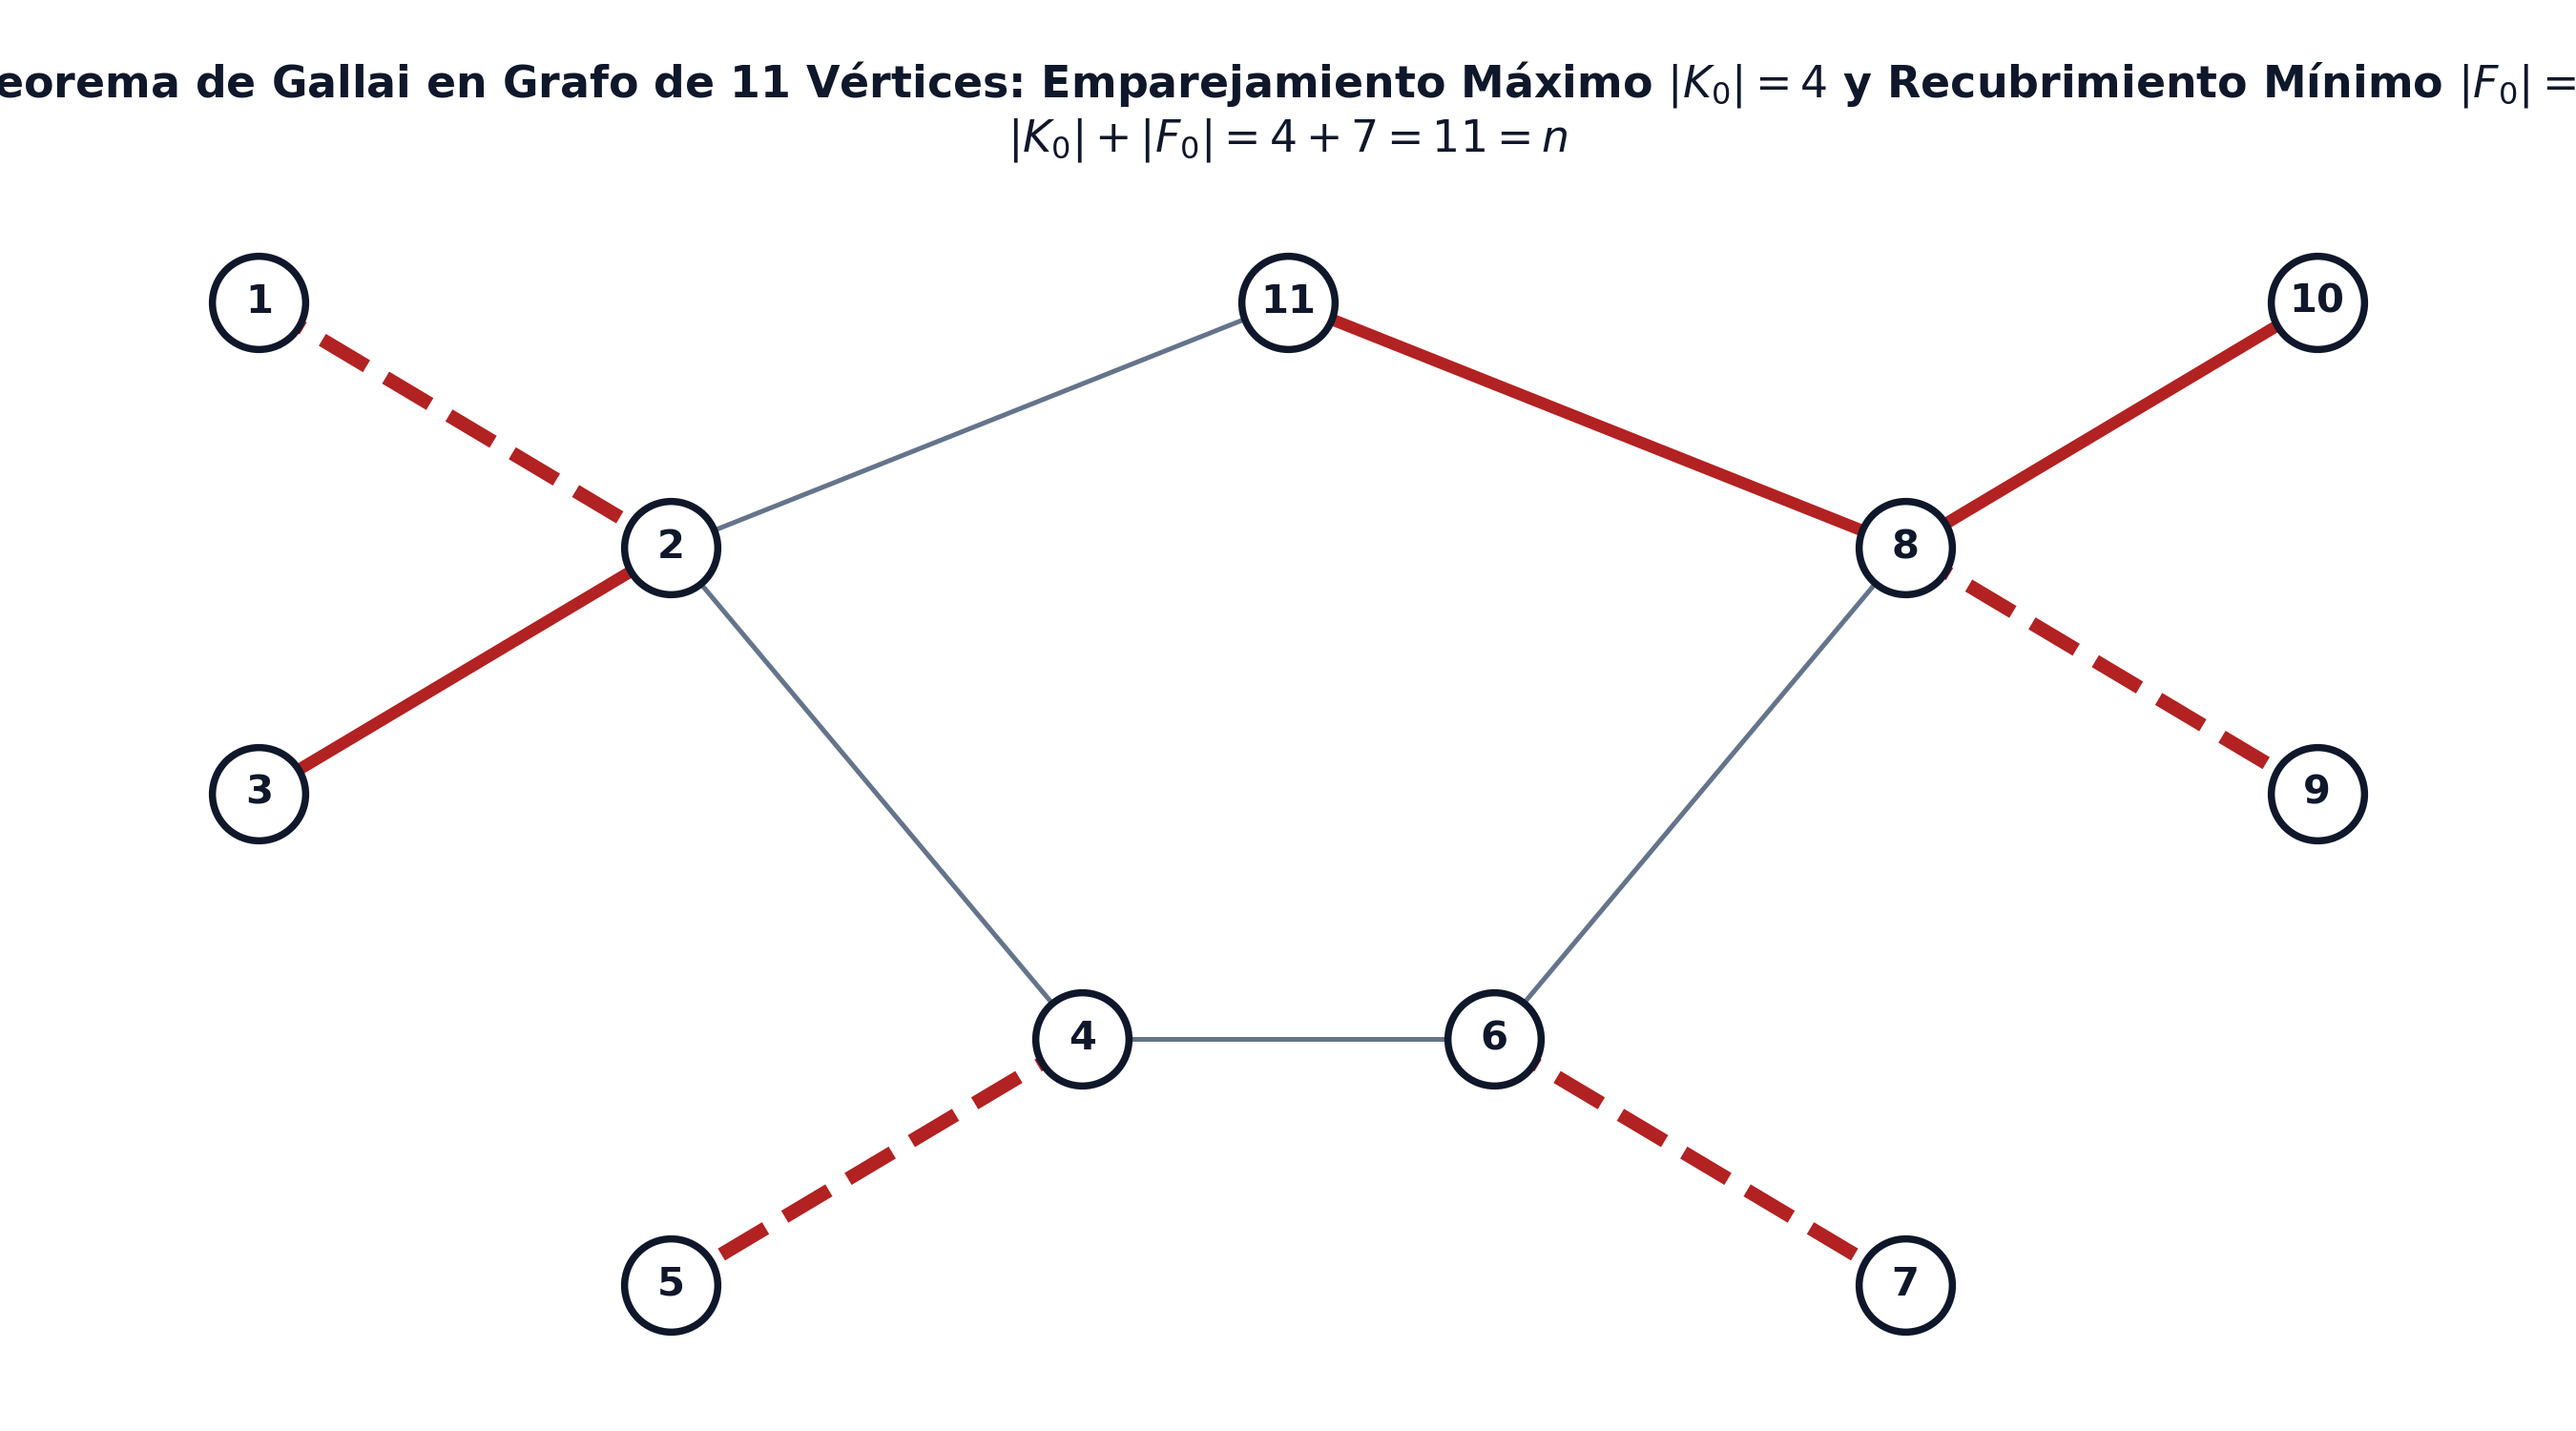
\includegraphics[width=0.85\linewidth,height=\textheight,keepaspectratio]{images/gallai_teorema_demostracion.png}

}

\caption{\label{fig-gallai-teorema-demostracion}Ilustración del Teorema
de Gallai en un grafo de 11 vértices: emparejamiento máximo \(|K_0|=4\)
(discontinuo) y recubrimiento mínimo \(|F_0|=7\) (rojo), verificando
\(|K_0| + |F_0| = 4 + 7 = 11\)}

\end{figure}%

\section{Emparejamiento de máximo peso y algoritmo
primal-dual}\label{emparejamiento-de-muxe1ximo-peso-y-algoritmo-primal-dual}

En múltiples aplicaciones logísticas, económicas y de
telecomunicaciones, las conexiones no tienen la misma importancia ni el
mismo rendimiento económico. En tales escenarios, cada arista
\(e \in E\) lleva asignado un peso o beneficio \(p(e) \in \mathbb{R}\),
y el objetivo no es maximizar el número de parejas, sino el \textbf{peso
total acumulado}.

\begin{tcolorbox}[enhanced jigsaw, toprule=.15mm, opacitybacktitle=0.6, coltitle=black, colbacktitle=quarto-callout-note-color!10!white, title=\textcolor{quarto-callout-note-color}{\faInfo}\hspace{0.5em}{Definición: Problema de emparejamiento de máximo peso}, arc=.35mm, rightrule=.15mm, toptitle=1mm, breakable, bottomtitle=1mm, titlerule=0mm, colback=white, opacityback=0, leftrule=.75mm, colframe=quarto-callout-note-color-frame, left=2mm, bottomrule=.15mm]

Dado un grafo simple no dirigido \(G = (V, E)\) y un vector de pesos
\(\mathbf{p} = \{p(e) \mid e \in E\}\), el \textbf{problema de
emparejamiento de máximo peso} consiste en determinar un subconjunto de
aristas \(K \subseteq E\) tal que:

\begin{enumerate}
\def\labelenumi{\arabic{enumi}.}
\tightlist
\item
  \(K\) es un emparejamiento válido de \(G\).
\item
  Para cualquier otro emparejamiento \(K' \subseteq E\), se satisface:
  \[
  p(K') \le p(K), \quad \text{donde } p(K) = \sum_{e \in K} p(e)
  \]
\end{enumerate}

\end{tcolorbox}

En el emparejamiento de máximo peso, un emparejamiento óptimo no tiene
por qué tener el máximo número de aristas posible: en ocasiones, el
beneficio máximo se obtiene con menos aristas si estas concentran pesos
individuales muy superiores.

\subsection{Coste reducido de cadenas y caracterización de
optimalidad}\label{coste-reducido-de-cadenas-y-caracterizaciuxf3n-de-optimalidad}

Para cuantificar el impacto económico de alterar un emparejamiento a lo
largo de una cadena alternante, definimos el concepto de coste reducido.

\begin{tcolorbox}[enhanced jigsaw, toprule=.15mm, opacitybacktitle=0.6, coltitle=black, colbacktitle=quarto-callout-note-color!10!white, title=\textcolor{quarto-callout-note-color}{\faInfo}\hspace{0.5em}{Definición: Coste reducido de una cadena alternante}, arc=.35mm, rightrule=.15mm, toptitle=1mm, breakable, bottomtitle=1mm, titlerule=0mm, colback=white, opacityback=0, leftrule=.75mm, colframe=quarto-callout-note-color-frame, left=2mm, bottomrule=.15mm]

Dado un grafo \(G = (V, E)\) con pesos \(p(e)\), un emparejamiento
\(K \subseteq E\) y una cadena alternante \(L\), se define el
\textbf{coste reducido} de \(L\) respecto de \(K\), denotado por
\(\delta_L\), como:

\[
\delta_L = p(L \cap \overline{K}) - p(L \cap K) = \sum_{e \in L \setminus K} p(e) - \sum_{e \in L \cap K} p(e)
\]

donde \(\overline{K} = E \setminus K\) representa el conjunto de aristas
fuera del emparejamiento.

\end{tcolorbox}

\begin{tcolorbox}[enhanced jigsaw, toprule=.15mm, opacitybacktitle=0.6, coltitle=black, colbacktitle=quarto-callout-note-color!10!white, title=\textcolor{quarto-callout-note-color}{\faInfo}\hspace{0.5em}{Definición: Ciclo alternante}, arc=.35mm, rightrule=.15mm, toptitle=1mm, breakable, bottomtitle=1mm, titlerule=0mm, colback=white, opacityback=0, leftrule=.75mm, colframe=quarto-callout-note-color-frame, left=2mm, bottomrule=.15mm]

Dado un grafo \(G = (V, E)\) y un emparejamiento \(K \subseteq E\), un
\textbf{ciclo alternante} es una cadena alternante cerrada y simple de
longitud estrictamente par, cuyas aristas pertenecen y no pertenecen
alternativamente al emparejamiento \(K\).

\end{tcolorbox}

El signo del coste reducido \(\delta_L\) posee una interpretación
económica directa: representa el beneficio marginal neto obtenido al
intercambiar las parejas existentes a lo largo de \(L\):

\begin{itemize}
\tightlist
\item
  Si \(\delta_L > 0\), la transferencia \textbf{incrementa
  estrictamente} el peso de la solución (\(p(K') = p(K) + \delta_L\)).
\item
  Si \(\delta_L = 0\), la transferencia mantiene invariable el peso
  acumulado.
\item
  Si \(\delta_L < 0\), la transferencia empeora el peso total.
\end{itemize}

\begin{tcolorbox}[enhanced jigsaw, toprule=.15mm, opacitybacktitle=0.6, coltitle=black, colbacktitle=quarto-callout-important-color!10!white, title=\textcolor{quarto-callout-important-color}{\faExclamation}\hspace{0.5em}{Teorema: Optimalidad por costes reducidos}, arc=.35mm, rightrule=.15mm, toptitle=1mm, breakable, bottomtitle=1mm, titlerule=0mm, colback=white, opacityback=0, leftrule=.75mm, colframe=quarto-callout-important-color-frame, left=2mm, bottomrule=.15mm]

Dado un grafo \(G = (V, E)\) con pesos \(p(e)\) sobre las aristas, un
emparejamiento \(K \subseteq E\) es de \textbf{máximo peso} si y solo si
\textbf{no existe ninguna cadena alternante} (abierta o cerrada) con
coste reducido estrictamente positivo (\(\delta_L \le 0\) para toda
cadena alternante \(L\)).

\emph{Demostración}:

\begin{itemize}
\tightlist
\item
  \textbf{Necesidad (\(\implies\))}: Si existiera una cadena alternante
  \(L\) con \(\delta_L > 0\), la transferencia
  \(K' = K \bigtriangleup L\) produciría un emparejamiento de peso
  \(p(K') = p(K) + \delta_L > p(K)\), lo que contradice la optimalidad
  de \(K\).
\item
  \textbf{Suficiencia (\(\impliedby\))}: Sea \(K_1\) un emparejamiento
  de máximo peso global, de modo que \(p(K_1) \ge p(K)\). Consideramos
  el grafo diferencia simétrica \(H = (V, K \bigtriangleup K_1)\). Por
  el Lema de Descomposición, \(H\) se descompone en vértices aislados,
  ciclos alternantes y cadenas alternantes respecto de \(K\). Al no
  existir en \(G\) ninguna cadena ni ciclo alternante con coste reducido
  positivo respecto de \(K\), la suma de las diferencias de peso sobre
  todas las componentes de \(H\) satisface
  \(p(K_1) - p(K) \le 0 \implies p(K_1) \le p(K)\). Por consiguiente,
  \(p(K) = p(K_1)\), lo que certifica que \(K\) es de máximo peso.
  \(\blacksquare\)
\end{itemize}

\end{tcolorbox}

Este teorema generaliza el criterio de Berge: mientras que para
emparejamientos de máximo cardinal se busca cualquier cadena incremental
(que siempre aporta \(+1\) arista neta), en el caso ponderado se buscan
cadenas que aporten un balance de peso neto positivo (\(\delta_L > 0\)).

\subsection{Algoritmo de aumento por cardinalidad
fija}\label{algoritmo-de-aumento-por-cardinalidad-fija}

La resolución algorítmica del emparejamiento de máximo peso se
estructura determinando inductivamente los emparejamientos \(K^m\) de
máximo peso para cada cardinalidad fija
\(m = 1, 2, \dots, \lfloor n/2 \rfloor\):

\begin{itemize}
\tightlist
\item
  \(K^1\): Es la arista individual de mayor peso en \(E\).
\item
  \(K^2\): Es el par de aristas disjuntas de mayor suma de pesos en
  \(E\).
\item
  \(K^{m+1}\): Se obtiene a partir de \(K^m\) mediante el siguiente
  resultado teórico fundamental.
\end{itemize}

\begin{tcolorbox}[enhanced jigsaw, toprule=.15mm, opacitybacktitle=0.6, coltitle=black, colbacktitle=quarto-callout-important-color!10!white, title=\textcolor{quarto-callout-important-color}{\faExclamation}\hspace{0.5em}{Teorema: Progresión de emparejamientos de peso máximo}, arc=.35mm, rightrule=.15mm, toptitle=1mm, breakable, bottomtitle=1mm, titlerule=0mm, colback=white, opacityback=0, leftrule=.75mm, colframe=quarto-callout-important-color-frame, left=2mm, bottomrule=.15mm]

Sea \(G = (V, E)\) un grafo, sea \(K^m\) el emparejamiento de máximo
peso entre todos los de cardinal \(m\), y sea \(L\) una \textbf{cadena
alternante incremental} respecto de \(K^m\) que posea el \textbf{coste
reducido máximo} (\(\delta(L) = \max \delta\)).

Entonces, el emparejamiento \(K^{m+1} = K^m \bigtriangleup L\) obtenido
por la transferencia de \(L\) es el \textbf{emparejamiento de máximo
peso entre todos los de cardinal \(m + 1\)}.

\emph{Demostración}: Sea \(K^*\) un emparejamiento óptimo de peso máximo
con exactamente \(m + 1\) aristas. Analizamos el subgrafo diferencia
simétrica: \[
H = (V, E_H), \quad \text{donde } E_H = (K^* \setminus K^m) \cup (K^m \setminus K^*)
\]

El grafo \(H\) se compone exclusivamente de vértices aislados, ciclos
alternantes y cadenas alternantes:

\begin{enumerate}
\def\labelenumi{\arabic{enumi}.}
\tightlist
\item
  Los ciclos alternantes y las cadenas alternantes de longitud par
  poseen igual número de aristas de \(K^*\) que de \(K^m\). Al ser
  \(K^*\) y \(K^m\) óptimos en sus respectivas cardinalidades, el coste
  reducido de todas estas componentes cerradas o pares es exactamente
  \(0\).
\item
  Para las cadenas alternantes de longitud impar, decimos que una cadena
  está \textbf{dominada por \(K^*\)} si contiene más aristas de \(K^*\)
  que de \(K^m\) (es decir, \(k+1\) aristas de \(K^*\) y \(k\) aristas
  de \(K^m\)), y \textbf{dominada por \(K^m\)} en caso contrario.
\end{enumerate}

Dado que \(|K^*| = |K^m| + 1\), el número de aristas de \(K^*\) en \(H\)
supera en exactamente \(1\) al número de aristas de \(K^m\). En
consecuencia, si existen \(s\) cadenas impares dominadas por \(K^m\),
debe haber exactamente \(s + 1\) cadenas impares dominadas por \(K^*\).
Las \(s\) cadenas dominadas por \(K^m\) se pueden emparejar y compensar
con \(s\) cadenas dominadas por \(K^*\). Por la optimalidad de ambas
soluciones, estas \(2s\) cadenas compensadas tienen coste reducido total
nulo.

Queda exactamente \textbf{una única cadena impar no compensada},
denotada por \(L^*\), que está dominada por \(K^*\). Al tener sus
extremos libres en \(K^m\), \(L^*\) es una \textbf{cadena alternante
incremental} respecto de \(K^m\). Dicha cadena concentra toda la
diferencia neta de peso entre \(K^*\) y \(K^m\): \[
p(K^*) = p(K^m) + \delta(L^*)
\]

Por otro lado, por definición de \(K^{m+1} = K^m \bigtriangleup L\), su
peso es: \[
p(K^{m+1}) = p(K^m) + \delta(L)
\]

Como \(K^*\) es el emparejamiento de peso máximo con \(m + 1\) aristas,
se tiene \(p(K^{m+1}) \le p(K^*) \implies \delta(L) \le \delta(L^*)\).
Pero habiendo seleccionado \(L\) como la cadena de coste reducido máximo
en \(G\), se cumple \(\delta(L) \ge \delta(L^*)\). Por tanto,
\(\delta(L) = \delta(L^*)\) y \(p(K^{m+1}) = p(K^*)\), lo que demuestra
que \(K^{m+1}\) es un emparejamiento de máximo peso de cardinal
\(m + 1\). \(\blacksquare\)

\end{tcolorbox}

\begin{tcolorbox}[enhanced jigsaw, toprule=.15mm, opacitybacktitle=0.6, coltitle=black, colbacktitle=quarto-callout-tip-color!10!white, title=\textcolor{quarto-callout-tip-color}{\faLightbulb}\hspace{0.5em}{Ejemplo: Resolución de emparejamiento de peso máximo en grafo de 6 nodos}, arc=.35mm, rightrule=.15mm, toptitle=1mm, breakable, bottomtitle=1mm, titlerule=0mm, colback=white, opacityback=0, leftrule=.75mm, colframe=quarto-callout-tip-color-frame, left=2mm, bottomrule=.15mm]

Considérese el grafo de 6 vértices \(V = \{1, 2, 3, 4, 5, 6\}\) y 9
aristas ponderadas representado en la \textbf{?@fig-peso-animado}, cuyos
pesos se dividen en dos conjuntos de aristas: \[
\begin{aligned}
& p(1,2)=2, \quad p(1,6)=1, \quad p(6,2)=2, \quad p(6,3)=3, \quad p(2,3)=3, \\
& p(2,4)=1, \quad p(3,4)=4, \quad p(4,5)=5, \quad p(6,5)=2
\end{aligned}
\]

Aplicamos el algoritmo de aumento inductivo por cardinalidad:

\begin{enumerate}
\def\labelenumi{\arabic{enumi}.}
\tightlist
\item
  \textbf{Cardinal \(m = 1\)}:

  \begin{itemize}
  \item
    Buscamos la arista de peso máximo en \(E\):
    \[e^* = \{4, 5\} \quad \text{con } p(4, 5) = 5\]
  \item
    Obtenemos el emparejamiento óptimo de 1 arista:
    \[K^1 = \bigl\{ \{4, 5\} \bigr\}, \quad p(K^1) = 5\]
  \end{itemize}
\item
  \textbf{Cardinal \(m = 2\)}:

  \begin{itemize}
  \tightlist
  \item
    Los vértices expuestos respecto de \(K^1\) son \(\{1, 2, 3, 6\}\).
  \item
    Buscamos entre los vértices expuestos la cadena incremental \(L_1\)
    que maximice el coste reducido \(\delta(L_1)\). Evaluamos aristas
    disjuntas a \(\{4,5\}\):

    \begin{itemize}
    \tightlist
    \item
      Arista \(\{2, 3\}\): \(\delta = p(2, 3) = 3\).
    \item
      Arista \(\{6, 3\}\): \(\delta = p(6, 3) = 3\).
    \item
      Arista \(\{1, 2\}\): \(\delta = p(1, 2) = 2\).
    \end{itemize}
  \item
    Seleccionamos la arista de mayor incremento \(L_1 = \{2, 3\}\) con
    \(\delta(L_1) = 3\).
  \item
    Obtenemos el emparejamiento óptimo de 2 aristas:
    \[K^2 = K^1 \cup \bigl\{ \{2, 3\} \bigr\} = \bigl\{ \{4, 5\}, \, \{2, 3\} \bigr\}, \quad p(K^2) = 5 + 3 = 8\]
  \end{itemize}
\item
  \textbf{Cardinal \(m = 3\)}:

  \begin{itemize}
  \tightlist
  \item
    Los vértices expuestos respecto de \(K^2\) son \(\{1, 6\}\).
  \item
    Evaluamos todas las cadenas incrementales alternantes que conectan
    los vértices expuestos \(1\) y \(6\):

    \begin{itemize}
    \item
      \textbf{Cadena de longitud 1} (\(L_A = 1 - 6\)):
      \[\delta(L_A) = p(1, 6) = 1\]
    \item
      \textbf{Cadena de longitud 3} (\(L_B = 1 - 2 - 3 - 6\)): Entran
      las aristas \(\{1,2\}\) y \(\{3,6\}\); sale la arista
      \(\{2,3\} \in K^2\): \[
      \begin{aligned}
      \delta(L_B) &= [p(1,2) + p(3,6)] - p(2,3) \\
      &= [2 + 3] - 3 = 2
      \end{aligned}
      \]
    \item
      \textbf{Cadena de longitud 5} (\(L_C = 1 - 2 - 3 - 4 - 5 - 6\)):
      Entran las aristas \(\{1,2\}\), \(\{3,4\}\) y \(\{6,5\}\); salen
      las aristas \(\{2,3\}\) y \(\{4,5\} \in K^2\): \[
      \begin{aligned}
      \delta(L_C) &= [p(1,2) + p(3,4) + p(6,5)] - [p(2,3) + p(4,5)] \\
      &= [2 + 4 + 2] - [3 + 5] = 8 - 8 = 0
      \end{aligned}
      \]
    \end{itemize}
  \item
    El coste reducido máximo es \(\delta(L_B) = 2\), correspondiente a
    la cadena alternante \(L_B = 1 - 2 - 3 - 6\).
  \item
    Realizamos la transferencia
    \(K^3 = K^2 \bigtriangleup (1-2-3-6) = \bigl( K^2 \setminus \{\{2,3\}\} \bigr) \cup \bigl\{ \{1,2\}, \{3,6\} \bigr\}\):
    \[
    K^3 = \bigl\{ \{1, 2\}, \, \{3, 6\}, \, \{4, 5\} \bigr\}, \quad p(K^3) = p(K^2) + \delta(L_B) = 8 + 2 = 10
    \]
  \end{itemize}
\item
  \textbf{Conclusión de Optimalidad Global}: Dado que \(K^3\) es un
  emparejamiento perfecto (satura los 6 vértices del grafo), no es
  posible construir emparejamientos con un número mayor de aristas. El
  \textbf{emparejamiento de peso máximo global} es: \[
  K^* = K^3 = \bigl\{ \{1, 2\}, \, \{3, 6\}, \, \{4, 5\} \bigr\} \quad \text{con peso óptimo total } p(K^*) = 10
  \]
\end{enumerate}

\end{tcolorbox}

\chapter{Rutas eulerianas, hamiltonianas y problemas de
rutas}\label{rutas-eulerianas-hamiltonianas-y-problemas-de-rutas}

El diseño y optimización de rutas sobre redes valoradas constituye uno
de los pilares más fascinantes y de mayor repercusión industrial de la
investigación operativa, la ciencia de la computación y la logística
moderna (Papadimitriou y Steiglitz 1998; Wolsey 1998). Desde una
perspectiva teórica y algorítmica, los problemas de recorridos permiten
estudiar la profunda frontera que separa los problemas resolubles en
tiempo polinomial (clase \(\mathcal{P}\)), como la determinación de
trayectorias que inspeccionan la totalidad de las aristas o calles de
una red (el \textbf{Problema del Cartero Chino}), frente a los problemas
computacionalmente intratables de naturaleza \(\mathcal{NP}\)-completa y
\(\mathcal{NP}\)-dura, como la secuenciación óptima de visitas a un
conjunto de clientes o nodos sin repetición (el \textbf{Problema del
Viajante de Comercio} o TSP, y sus extensiones multi-vehículo VRP).

En este capítulo, desarrollaremos de forma rigurosa la teoría matemática
y las técnicas algorítmicas que sustentan el análisis de recorridos en
grafos. Comenzaremos explorando los orígenes históricos de la teoría de
grafos en los puentes de Königsberg y la caracterización exacta de los
\textbf{grafos eulerianos}, formalizando un algoritmo constructivo de
cadenas eulerianas basado en estructuras de punteros. A continuación,
estudiaremos el \textbf{Problema del Cartero Chino (CPP)} en redes no
eulerianas, demostrando la descomposición de aristas duplicadas y
resolviendo el modelo mediante emparejamientos perfectos de peso mínimo.
Posteriormente, abordaremos los \textbf{ciclos hamiltonianos},
analizando la condición necesaria de 2-conexidad, la proposición
fundamental de adyacencia y el Teorema de la \textbf{Clausura de Bondy y
Chvátal}. Seguidamente, formularemos el \textbf{Problema del Viajante
(TSP)} mediante tres modelos lineales enteros fundamentales (el modelo
tridimensional por tramos, la formulación con eliminación exponencial de
subciclos de Dantzig-Fulkerson-Johnson y el modelo polinomial compacto
de Miller-Tucker-Zemlin), analizando además heurísticas locales (2-opt)
y el algoritmo de aproximación métrica de \textbf{Christofides} con la
demostración de su garantía de factor \(1.5\). Finalmente,
estableceremos la taxonomía global de los \textbf{Problemas de Rutas de
Vehículos (VRP)} y sus múltiples variantes operativas.

\begin{tcolorbox}[enhanced jigsaw, toprule=.15mm, opacitybacktitle=0.6, coltitle=black, colbacktitle=quarto-callout-important-color!10!white, title=\textcolor{quarto-callout-important-color}{\faExclamation}\hspace{0.5em}{Objetivos de aprendizaje}, arc=.35mm, rightrule=.15mm, toptitle=1mm, breakable, bottomtitle=1mm, titlerule=0mm, colback=white, opacityback=0, leftrule=.75mm, colframe=quarto-callout-important-color-frame, left=2mm, bottomrule=.15mm]

Al finalizar este capítulo, serás capaz de:

\begin{enumerate}
\def\labelenumi{\arabic{enumi}.}
\tightlist
\item
  \textbf{Diferenciar} formalmente entre grafos eulerianos (recorridos
  por aristas en tiempo polinomial) y grafos hamiltonianos (recorridos
  por vértices de complejidad \(\mathcal{NP}\)-completa).
\item
  \textbf{Aplicar} el teorema fundamental de caracterización de Euler y
  ejecutar el algoritmo constructivo de punteros para determinar cadenas
  y ciclos eulerianos.
\item
  \textbf{Formular y resolver} el Problema del Cartero Chino (CPP) sobre
  grafos generales, modelando la eulerización óptima mediante
  emparejamientos perfectos de peso mínimo sobre el grafo auxiliar de
  nodos impares.
\item
  \textbf{Demostrar} la proposición fundamental de adyacencia
  hamiltoniana y evaluar la existencia de ciclos hamiltonianos mediante
  el operador de clausura de Bondy-Chvátal y los teoremas clásicos de
  Dirac y Ore.
\item
  \textbf{Formular} el Problema del Viajante (TSP) comparando las
  formulaciones de eliminación exponencial de subtours (DFJ) y la
  formulación polinomial compacta (MTZ), justificando el compromiso
  entre fortaleza poliédrica y dimensión.
\item
  \textbf{Clasificar} los problemas generales de rutas de vehículos
  (VRP/VSP, rutas por nodos frente a rutas por arcos) identificando sus
  dimensiones operativas (flotas, depósitos, demandas, ventanas de
  tiempo y funciones objetivo).
\end{enumerate}

\end{tcolorbox}

\begin{center}\rule{0.5\linewidth}{0.5pt}\end{center}

\section{Grafos eulerianos y el problema de los puentes de
Königsberg}\label{grafos-eulerianos-y-el-problema-de-los-puentes-de-kuxf6nigsberg}

El nacimiento formal de la teoría de grafos y de la topología matemática
se sitúa en 1736, cuando el célebre matemático suizo \textbf{Leonhard
Euler} presentó en la Academia de San Petersburgo su memoria titulada
\emph{Solutio Problematis ad Geometriam Situs Pertinentis} (Euler 1741).
En dicho trabajo, Euler abordó el célebre enigma planteado por los
ciudadanos de la ciudad prusiana de \textbf{Königsberg} (actual
Kaliningrado), atravesada por el río Pregel, el cual dividía la urbe en
cuatro masas terrestres conectadas entre sí mediante siete puentes. El
problema consistía en determinar si era posible diseñar un paseo urbano
que recorriera la ciudad cruzando \textbf{cada uno de los siete puentes
exactamente una vez y regresando al punto de partida}.

Euler demostró de forma analítica que tal recorrido cerrado era
físicamente imposible. Su genialidad radicó en abstraer por completo los
detalles geométricos (longitudes de calles, formas de las orillas o
distancias reales) y modelar la topología del sistema mediante un
\textbf{multigrafo}, donde las cuatro regiones terrestres se
representaban como vértices (\(A, B, C, D\)) y los siete puentes como
aristas que conectaban dichas regiones, tal como se ilustra en la
Figura~\ref{fig-puentes-konigsberg-grafo}.

\begin{figure}

\centering{

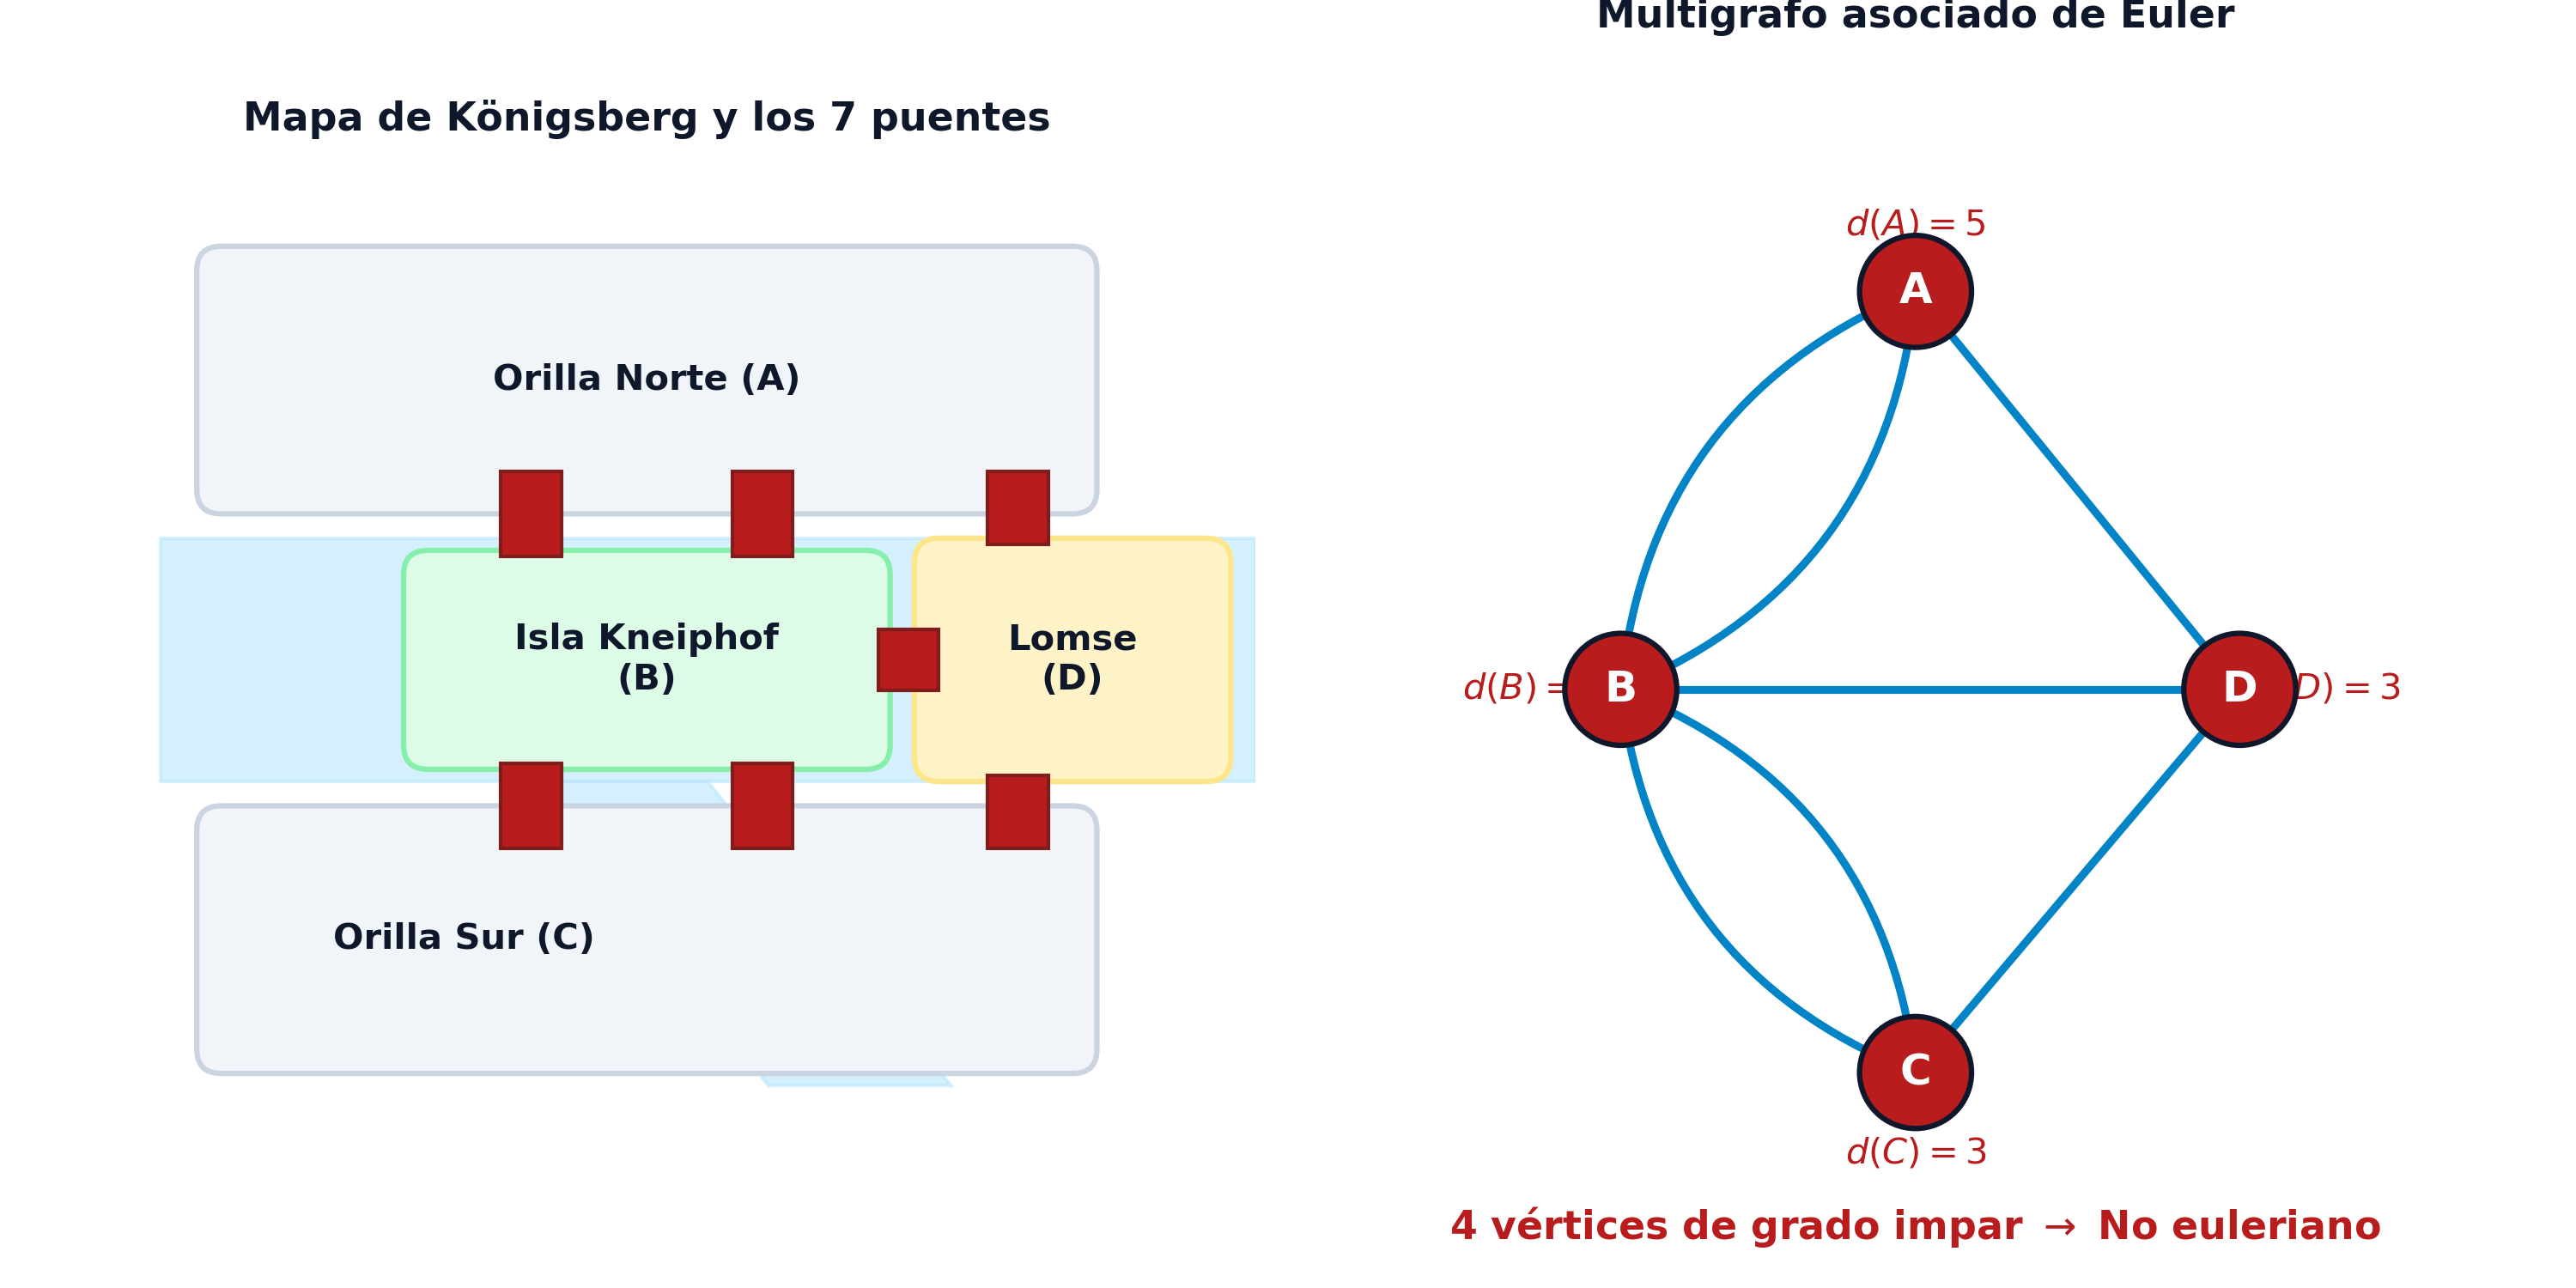
\includegraphics[width=0.95\linewidth,height=\textheight,keepaspectratio]{images/puentes_konigsberg_grafo.png}

}

\caption{\label{fig-puentes-konigsberg-grafo}El problema de los siete
puentes de Königsberg: mapa fluvial sobre el río Pregel (izquierda) y
multigrafo abstracto de Euler con los grados nodales asociados
(derecha)}

\end{figure}%

El análisis de Euler demostró que, para que un vértice cualquiera actúe
como punto de paso intermedio de un recorrido continuo sin repetir
puentes, cada vez que el caminante entra en dicho vértice por un puente
debe existir necesariamente otro puente disponible sin cruzar para salir
de él. En consecuencia, cada visita intermedia consume exactamente dos
conexiones, lo que exige que el número de aristas incidentes en cada
nodo intermedio (\textbf{grado del vértice}) sea obligatoriamente un
\textbf{número par}.

\begin{tcolorbox}[enhanced jigsaw, toprule=.15mm, opacitybacktitle=0.6, coltitle=black, colbacktitle=quarto-callout-note-color!10!white, title=\textcolor{quarto-callout-note-color}{\faInfo}\hspace{0.5em}{Definición: Cadenas y ciclos eulerianos}, arc=.35mm, rightrule=.15mm, toptitle=1mm, breakable, bottomtitle=1mm, titlerule=0mm, colback=white, opacityback=0, leftrule=.75mm, colframe=quarto-callout-note-color-frame, left=2mm, bottomrule=.15mm]

Dado un multigrafo finito conexo no dirigido \(G = (V, E)\):

\begin{itemize}
\tightlist
\item
  \textbf{Cadena euleriana}: Es una secuencia ordenada de vértices y
  aristas que recorre \textbf{todas las aristas} del conjunto \(E\)
  pasando por cada una de ellas \textbf{exactamente una vez} (sin
  repetir ninguna arista).
\item
  \textbf{Ciclo euleriano}: Es una cadena euleriana \textbf{cerrada}, es
  decir, una cadena euleriana cuyo vértice inicial coincide con su
  vértice final.
\item
  \textbf{Grafo euleriano}: Un multigrafo \(G = (V, E)\) se denomina
  \textbf{euleriano} si admite al menos un ciclo euleriano.
\end{itemize}

\end{tcolorbox}

La caracterización matemática completa de la existencia de tales
trayectorias sobre redes conexas se formaliza en el teorema fundamental
de Euler, extendido posteriormente por Carl Hierholzer en 1873.

\begin{tcolorbox}[enhanced jigsaw, toprule=.15mm, opacitybacktitle=0.6, coltitle=black, colbacktitle=quarto-callout-important-color!10!white, title=\textcolor{quarto-callout-important-color}{\faExclamation}\hspace{0.5em}{Teorema: Teorema de Euler de caracterización euleriana}, arc=.35mm, rightrule=.15mm, toptitle=1mm, breakable, bottomtitle=1mm, titlerule=0mm, colback=white, opacityback=0, leftrule=.75mm, colframe=quarto-callout-important-color-frame, left=2mm, bottomrule=.15mm]

Sea \(G = (V, E)\) un multigrafo finito y conexo. Entonces:

\begin{enumerate}
\def\labelenumi{\arabic{enumi}.}
\item
  \(G\) contiene un \textbf{ciclo euleriano} si y solo si \textbf{todos
  los vértices de \(V\) tienen grado par}: \[
  d(i) \equiv 0 \pmod 2, \quad \forall i \in V
  \]
\item
  \(G\) contiene una \textbf{cadena euleriana abierta} (no cerrada) si y
  solo si el número de vértices de grado impar es \textbf{exactamente
  dos}. En tal caso, los dos vértices de grado impar constituyen
  necesariamente los extremos inicial y final de la cadena.
\end{enumerate}

\emph{Demostración}: Demostremos en primer lugar la condición necesaria
para la existencia de un ciclo euleriano. Supongamos que \(G\) admite un
ciclo euleriano \(C\). Al recorrer el ciclo arista por arista desde el
origen hasta el retorno final, cada paso a través de un vértice
intermedio \(i \in V\) utiliza una arista entrante y otra arista
saliente no explorada previamente. Por tanto, cada tránsito a través de
\(i\) incrementa su grado local en dos unidades. Como todas las aristas
de \(E\) son visitadas exactamente una vez, el grado total \(d(i)\) de
cada vértice es el doble del número de veces que el ciclo pasa por él,
resultando un número estrictamente par. Si la cadena es abierta y une
dos vértices distintos \(u\) y \(v\), el vértice inicial \(u\) tiene una
arista saliente neta adicional (grado impar), el vértice final \(v\)
tiene una arista entrante neta adicional (grado impar), y todos los
demás vértices intermedios conservan balance par de entrada y salida.

Para demostrar la suficiencia en el caso de que todos los vértices
tengan grado par, seleccionamos un vértice cualquiera \(v_0\) y
construimos un camino simple avanzando por aristas no utilizadas. Dado
que cada vértice tiene grado par, al entrar en cualquier vértice siempre
existirá al menos una arista libre para salir, a menos que regresemos al
vértice de partida \(v_0\). Así, se forma un ciclo inicial \(C_1\). Si
\(C_1\) contiene todas las aristas de \(E\), hemos terminado. Si no es
así, al ser \(G\) conexo, existe algún vértice \(v_k \in C_1\) que
incide en aristas no pertenecientes a \(C_1\). El subgrafo residual
\(G \setminus E(C_1)\) sigue teniendo todos sus vértices de grado par.
Repitiendo el proceso desde \(v_k\), obtenemos un nuevo ciclo \(C_2\)
que puede empalmarse en \(v_k\) dentro de \(C_1\). Reiterando esta
descomposición sobre el número finito de aristas, se obtiene un ciclo
euleriano que integra la totalidad de \(E\). \(\blacksquare\)

\end{tcolorbox}

En el multigrafo de los puentes de Königsberg mostrado en la
Figura~\ref{fig-puentes-konigsberg-grafo}, los grados de los cuatro
vértices son \(d(A)=5\), \(d(B)=3\), \(d(C)=3\) y \(d(D)=3\). Al existir
cuatro vértices de grado impar (ninguno con grado par), el teorema de
Euler certifica formalmente la imposibilidad de trazar ni un ciclo ni
una cadena euleriana abierta.

\begin{tcolorbox}[enhanced jigsaw, toprule=.15mm, opacitybacktitle=0.6, coltitle=black, colbacktitle=quarto-callout-note-color!10!white, title=\textcolor{quarto-callout-note-color}{\faInfo}\hspace{0.5em}{Nota: Distinción entre cadenas y ciclos eulerianos según la paridad}, arc=.35mm, rightrule=.15mm, toptitle=1mm, breakable, bottomtitle=1mm, titlerule=0mm, colback=white, opacityback=0, leftrule=.75mm, colframe=quarto-callout-note-color-frame, left=2mm, bottomrule=.15mm]

Es conveniente clarificar con precisión la relación entre la noción
general de \textbf{cadena euleriana} y la de \textbf{ciclo euleriano}:

\begin{itemize}
\tightlist
\item
  \textbf{Existencia de cadena euleriana en general}: Un grafo conexo
  admite una cadena euleriana (cerrada o abierta) si y solo si el número
  de vértices de grado impar pertenece al conjunto \(\{0, 2\}\).
\item
  \textbf{Caso \(|V_{\text{impar}}| = 0\) (Ciclo euleriano)}: Si todos
  los vértices tienen grado par, la cadena es \textbf{cerrada} (un ciclo
  euleriano) y puede iniciarse y concluirse en cualquier vértice
  arbitrario de la red.
\item
  \textbf{Caso \(|V_{\text{impar}}| = 2\) (Cadena euleriana abierta)}:
  La cadena es \textbf{abierta} (no puede cerrarse sobre sí misma sin
  duplicar aristas) y sus extremos inicial y final son obligatoriamente
  los dos únicos vértices con grado impar.
\item
  \textbf{Caso \(|V_{\text{impar}}| \ge 4\)}: No existe ninguna cadena
  euleriana, ni abierta ni cerrada (el caso de
  \(|V_{\text{impar}}| = 1\) o cualquier número impar de vértices
  impares es topológicamente imposible en cualquier grafo por el Lema
  del apretón de manos).
\end{itemize}

\end{tcolorbox}

\subsection{Algoritmo constructivo para la determinación de cadenas
eulerianas}\label{algoritmo-constructivo-para-la-determinaciuxf3n-de-cadenas-eulerianas}

Para determinar de forma computacional una cadena o ciclo euleriano en
un multigrafo que cumple las condiciones de Euler, se requiere una
estructura de datos algorítmica eficiente que permita extender un
recorrido inicial e insertar recursivamente los ciclos secundarios que
surjan en los vértices intermedios.

Presentamos a continuación el algoritmo formal de construcción de
cadenas eulerianas mediante un vector de punteros de aristas sucesoras
\(\mathbf{\sigma} = (\sigma(1), \dots, \sigma(m), \sigma(m+1))\), donde
\(m = |E|\) denota el número total de aristas del grafo. En esta
estructura, cada componente \(\sigma(e)\) almacena el identificador de
la arista que sigue a la arista \(e\) en la secuencia del recorrido, y
la posición auxiliar \(\sigma(m+1)\) almacena el índice de la primera
arista de la cadena.

\begin{tcolorbox}[enhanced jigsaw, toprule=.15mm, opacitybacktitle=0.6, coltitle=black, colbacktitle=quarto-callout-note-color!10!white, title=\textcolor{quarto-callout-note-color}{\faInfo}\hspace{0.5em}{Esquema: Algoritmo de construcción de cadenas y ciclos eulerianos}, arc=.35mm, rightrule=.15mm, toptitle=1mm, breakable, bottomtitle=1mm, titlerule=0mm, colback=white, opacityback=0, leftrule=.75mm, colframe=quarto-callout-note-color-frame, left=2mm, bottomrule=.15mm]

Dado un grafo conexo \(G = (V, E)\) con \(m = |E|\) aristas numeradas
\(\{1, 2, \dots, m\}\), sean las siguientes estructuras de datos y
parámetros auxiliares:

\begin{itemize}
\tightlist
\item
  \(d(i)\): Grado del vértice \(i \in V\).
\item
  \(w(i)\): Conjunto ordenado de aristas incidentes en el vértice \(i\).
\item
  \(\delta_i(e) = j\): Función de incidencia que devuelve el vértice
  opuesto al que conecta la arista \(e = \{i, j\}\) desde el nodo \(i\).
\item
  \(\alpha(i)\): Contador dinámico del número de aristas incidentes en
  \(i\) que aún \textbf{no han sido exploradas} (inicialmente
  \(\alpha(i) = d(i)\)).
\item
  \(v\): Longitud acumulada del recorrido actual (número de aristas
  incorporadas).
\item
  \(\phi(i)\): Identificador de la arista utilizada para alcanzar por
  primera vez el vértice \(i\) dentro de la cadena (para el vértice
  inicial \(a\), se define \(\phi(a) = m+1\)).
\end{itemize}

El procedimiento algorítmico se articula en cuatro pasos:

\begin{enumerate}
\def\labelenumi{\arabic{enumi}.}
\tightlist
\item
  \textbf{Paso 1 (Inicialización)}:

  \begin{itemize}
  \tightlist
  \item
    Si el grafo posee dos vértices de grado impar, se selecciona uno de
    ellos como vértice inicial \(a\) y el otro como vértice terminal
    \(b\) (fijando \(i = a\) y \(t = b\)). Si todos los vértices son
    pares, se escoge un vértice arbitrario fijando \(a = b\)
    (\(i = a, t = a\)).
  \item
    Inicializar \(\sigma(e) = 0\) para todo
    \(e \in \{1, \dots, m, m+1\}\), \(\alpha(i) = d(i)\) y
    \(\phi(j) = 0\) para todo \(j \in V \setminus \{a\}\), fijando
    \(\phi(a) = m+1\), \(v = 0\), \(e_1 = m+1\) y \(e_2 = -1\).
  \end{itemize}
\item
  \textbf{Paso 2 (Extensión secuencial del recorrido)}:

  \begin{itemize}
  \item
    Si \(\alpha(i) = 0\), ir al \textbf{Paso 4}.
  \item
    En caso contrario, sea \(e\) la arista que ocupa la posición actual
    \(\alpha(i)\) en la lista de incidencias \(w(i)\). Decrementar el
    contador: \(\alpha(i) \leftarrow \alpha(i) - 1\).
  \item
    Si \(e = e_1\) o \(\sigma(e) \neq 0\) (arista ya explorada en
    sentido inverso), repetir el \textbf{Paso 2}.
  \item
    En otro caso (arista nueva disponible): \[
    \begin{aligned}
    j &= \delta_i(e), \quad \phi(j) = e, \quad \sigma(e_1) = e, \\
    v &\leftarrow v + 1, \quad \alpha(j) \leftarrow \alpha(j) - 1, \quad i \leftarrow j
    \end{aligned}
    \]
  \item
    Si el nuevo nodo alcanzado es el nodo objetivo (\(i = t\)), ir al
    \textbf{Paso 3}. En caso contrario, actualizar la última arista
    incorporada \(e_1 \leftarrow e\) y continuar en el \textbf{Paso 2}.
  \end{itemize}
\item
  \textbf{Paso 3 (Cierre de subcadena y verificación de parada)}:

  \begin{itemize}
  \tightlist
  \item
    Enlazar la última arista con la continuación del ciclo:
    \(\sigma(e) = e_2\).
  \item
    Si la longitud total alcanza el número total de aristas (\(v = m\)),
    el algoritmo \textbf{FINALIZA con éxito}: el vector
    \(\mathbf{\sigma}\) describe la cadena euleriana completa.
  \item
    Si \(v < m\), quedan aristas no exploradas, por lo que se avanza al
    \textbf{Paso 4}.
  \end{itemize}
\item
  \textbf{Paso 4 (Búsqueda y empalme de ciclos adyacentes)}:

  \begin{itemize}
  \item
    Buscar un vértice \(k \in V\) que satisfaga simultáneamente:

    \begin{enumerate}
    \def\labelenumii{\arabic{enumii}.}
    \tightlist
    \item
      \(\alpha(k) \neq 0\) (le restan aristas incidentes sin explorar).
    \item
      \(\phi(k) \neq 0\) (es un vértice perteneciente a la cadena ya
      construida).
    \end{enumerate}
  \item
    Configurar los punteros de inserción para abrir un ciclo secundario
    en dicho nodo: \[
    i \leftarrow k, \quad t \leftarrow k, \quad e_1 \leftarrow \phi(k), \quad e_2 \leftarrow \sigma(e_1)
    \]
  \item
    Regresar al \textbf{Paso 2} para construir el ciclo euleriano
    adyacente que se intercalará en la posición de \(k\).
  \end{itemize}
\end{enumerate}

\end{tcolorbox}

En el siguiente ejemplo, analizamos la ejecución detallada de este
algoritmo sobre un grafo de 4 nodos.

\begin{tcolorbox}[enhanced jigsaw, toprule=.15mm, opacitybacktitle=0.6, coltitle=black, colbacktitle=quarto-callout-tip-color!10!white, title=\textcolor{quarto-callout-tip-color}{\faLightbulb}\hspace{0.5em}{Ejemplo: Construcción paso a paso de una cadena euleriana}, arc=.35mm, rightrule=.15mm, toptitle=1mm, breakable, bottomtitle=1mm, titlerule=0mm, colback=white, opacityback=0, leftrule=.75mm, colframe=quarto-callout-tip-color-frame, left=2mm, bottomrule=.15mm]

Consideremos el grafo conexo \(G = (V, E)\) de \(4\) vértices
\(V = \{a, b, c, d\}\) y \(4\) aristas \(E = \{1, 2, 3, 4\}\) ilustrado
en la Figura~\ref{fig-euler-algoritmo-traza} (panel izquierdo), cuyas
aristas e incidencias son:

\begin{itemize}
\tightlist
\item
  Arista 1: \(\{a, b\} \implies \delta_a(1) = b, \delta_b(1) = a\).
\item
  Arista 2: \(\{b, c\} \implies \delta_b(2) = c, \delta_c(2) = b\).
\item
  Arista 3: \(\{c, d\} \implies \delta_c(3) = d, \delta_d(3) = c\).
\item
  Arista 4: \(\{b, d\} \implies \delta_b(4) = d, \delta_d(4) = b\).
\end{itemize}

Evaluando los grados nodales: \[
d(a) = 1, \quad d(b) = 3, \quad d(c) = 2, \quad d(d) = 2
\] Al existir exactamente dos vértices de grado impar (\(a\) y \(b\)),
el teorema de Euler garantiza la existencia de una cadena euleriana
abierta que comenzará en \(a\) y finalizará en \(b\).

\begin{enumerate}
\def\labelenumi{\arabic{enumi}.}
\tightlist
\item
  \textbf{Inicialización (Paso 1)}:

  \begin{itemize}
  \tightlist
  \item
    Vértice inicial: \(i = a\), vértice final: \(t = b\).
  \item
    Arista ficticia de cabecera: \(m+1 = 5\). Punteros iniciales:
    \(e_1 = 5, e_2 = -1, v = 0\).
  \item
    Contadores: \(\alpha(a)=1, \alpha(b)=3, \alpha(c)=2, \alpha(d)=2\).
  \item
    Punteros de llegada:
    \(\phi(a) = 5, \phi(b)=0, \phi(c)=0, \phi(d)=0\).
  \end{itemize}
\item
  \textbf{Primera extensión (Paso 2)}:

  \begin{itemize}
  \item
    En \(i = a\), \(\alpha(a)=1\). Arista disponible \(e = 1\). Se
    actualiza \(\alpha(a) = 0\).
  \item
    Como \(e=1 \neq e_1=5\), se conecta la arista: \[
    \begin{aligned}
    j &= \delta_a(1) = b, \quad \phi(b) = 1, \quad \sigma(5) = 1, \\
    v &= 1, \quad \alpha(b) = 3 - 1 = 2, \quad i = b
    \end{aligned}
    \]
  \item
    Como el nodo actual \(b\) coincide con el destino \(t=b\), se deriva
    al \textbf{Paso 3}.
  \end{itemize}
\item
  \textbf{Cierre de tramo inicial (Paso 3)}:

  \begin{itemize}
  \tightlist
  \item
    Se fija \(\sigma(1) = e_2 = -1\).
  \item
    Como la longitud acumulada \(v = 1 < 4\), la cadena no está
    completa. Se pasa al \textbf{Paso 4}.
  \end{itemize}
\item
  \textbf{Búsqueda de vértice de bifurcación (Paso 4)}:

  \begin{itemize}
  \item
    Se evalúa el nodo \(k = b\): cumple \(\alpha(b) = 2 \neq 0\) y
    \(\phi(b) = 1 \neq 0\).
  \item
    Se reconfiguran los punteros para intercalar un ciclo cerrado en
    \(b\): \[
    i = b, \quad t = b, \quad e_1 = \phi(b) = 1, \quad e_2 = \sigma(1) = -1
    \]
  \item
    Se regresa al \textbf{Paso 2}.
  \end{itemize}
\item
  \textbf{Construcción del ciclo secundario (Pasos 2 y 3)}:

  \begin{itemize}
  \item
    \emph{Iteración desde \(b\)}: \(\alpha(b)=2\), arista
    \(e = w_2(b) = 4\). Se actualiza \(\alpha(b)=1\). \[
    \begin{aligned}
    j &= \delta_b(4) = d, \quad \phi(d) = 4, \quad \sigma(1) = 4, \\
    v &= 2, \quad \alpha(d) = 2 - 1 = 1, \quad i = d, \quad e_1 = 4
    \end{aligned}
    \]
  \item
    \emph{Iteración desde \(d\)}: \(\alpha(d)=1\), arista
    \(e = w_1(d) = 3\). Se actualiza \(\alpha(d)=0\). \[
    \begin{aligned}
    j &= \delta_d(3) = c, \quad \phi(c) = 3, \quad \sigma(4) = 3, \\
    v &= 3, \quad \alpha(c) = 2 - 1 = 1, \quad i = c, \quad e_1 = 3
    \end{aligned}
    \]
  \item
    \emph{Iteración desde \(c\)}: \(\alpha(c)=1\), arista
    \(e = w_1(c) = 2\). Se actualiza \(\alpha(c)=0\). \[
    \begin{aligned}
    j &= \delta_c(2) = b, \quad \phi(b) = 2, \quad \sigma(3) = 2, \\
    v &= 4, \quad \alpha(b) = 1 - 1 = 0, \quad i = b
    \end{aligned}
    \]
  \item
    Al alcanzar de nuevo el destino intermedio \(i = t = b\), se pasa al
    \textbf{Paso 3}: \[
    \sigma(2) = e_2 = -1
    \]
  \item
    Como la longitud acumulada \(v = 4 = m\), el algoritmo
    \textbf{termina con éxito}.
  \end{itemize}
\end{enumerate}

El vector resultante de punteros \(\mathbf{\sigma}\) es: \[
\mathbf{\sigma} = (\sigma(1), \sigma(2), \sigma(3), \sigma(4), \sigma(5)) = (4, -1, 2, 3, 1)
\] Siguiendo la cadena desde el puntero inicial
\(\sigma(5)=1 \to \sigma(1)=4 \to \sigma(4)=3 \to \sigma(3)=2 \to \sigma(2)=-1\),
la secuencia ordenada de aristas es \((1, 4, 3, 2)\), correspondiente a
la cadena euleriana de vértices: \[
a \xrightarrow{e=1} b \xrightarrow{e=4} d \xrightarrow{e=3} c \xrightarrow{e=2} b
\]

\begin{figure}[H]

\centering{

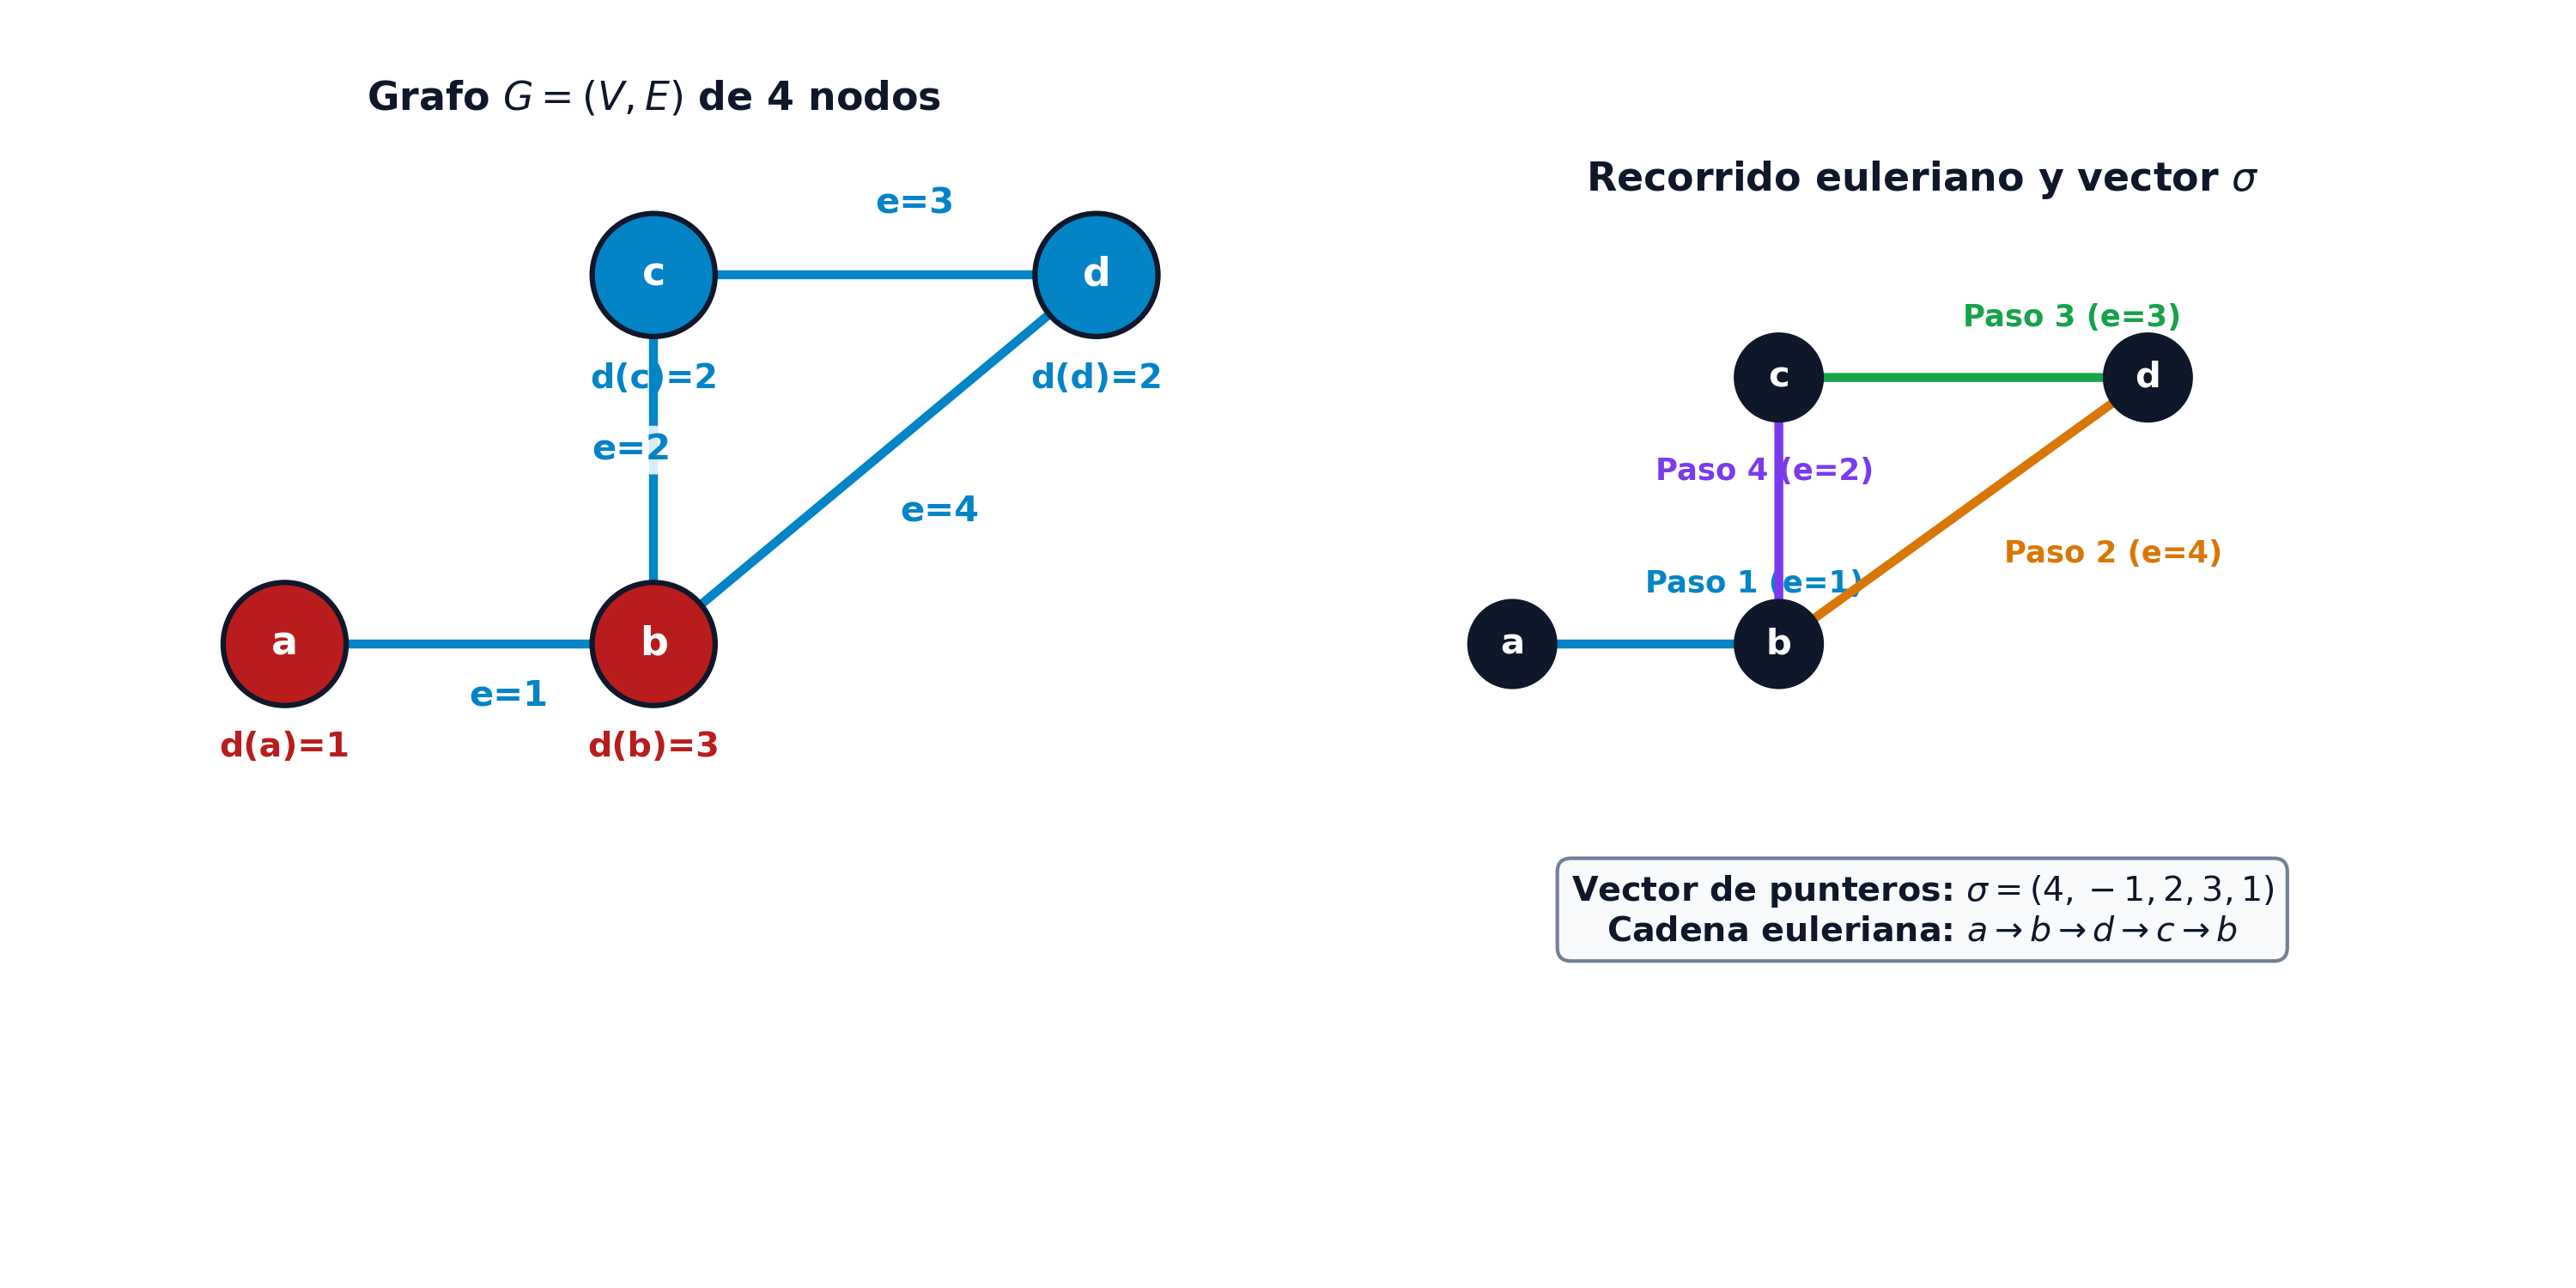
\includegraphics[width=0.85\linewidth,height=\textheight,keepaspectratio]{images/euler_algoritmo_traza.png}

}

\caption{\label{fig-euler-algoritmo-traza}Grafo de 4 nodos y traza
algorítmica de la cadena euleriana mediante el vector de punteros sigma}

\end{figure}%

\end{tcolorbox}

\begin{center}\rule{0.5\linewidth}{0.5pt}\end{center}

\section{El Problema del Cartero Chino
(CPP)}\label{el-problema-del-cartero-chino-cpp}

En la inmensa mayoría de las aplicaciones prácticas de transporte y
servicios urbanos (tales como el reparto postal a domicilio, la recogida
selectiva de residuos sólidos urbanos, la limpieza y barrido mecanizado
de calles, el esparcimiento de sal en vías nevadas o la inspección de
redes de tendido eléctrico y canalizaciones de agua), las redes viales
reales no son eulerianas, ya que suelen contener múltiples
intersecciones con un número impar de calles convergentes.

El \textbf{Problema del Cartero Chino} (conocido en la literatura
internacional como \emph{Chinese Postman Problem}, CPP, o problema del
circuito de inspección de aristas) plantea determinar el recorrido
cerrado de \textbf{longitud o coste total mínimo} que visite
\textbf{cada arista de la red al menos una vez}, regresando al punto de
partida (Kwan 1962). El problema fue formulado originalmente en 1960 por
el matemático chino \textbf{Mei-Ko Kwan}, y su denominación en lengua
inglesa fue propuesta en 1962 por el investigador operativo Alan J.
Goldman.

\begin{tcolorbox}[enhanced jigsaw, toprule=.15mm, opacitybacktitle=0.6, coltitle=black, colbacktitle=quarto-callout-note-color!10!white, title=\textcolor{quarto-callout-note-color}{\faInfo}\hspace{0.5em}{Definición: Problema del Cartero Chino (CPP)}, arc=.35mm, rightrule=.15mm, toptitle=1mm, breakable, bottomtitle=1mm, titlerule=0mm, colback=white, opacityback=0, leftrule=.75mm, colframe=quarto-callout-note-color-frame, left=2mm, bottomrule=.15mm]

Dada una red valorada no dirigida \(G = (V, E, p)\), donde \(V\) es el
conjunto de vértices, \(E\) es el conjunto de aristas y
\(p: E \to \mathbb{R}^+\) asigna un peso o longitud no negativa \(p(e)\)
a cada arista \(e \in E\):

El \textbf{Problema del Cartero Chino} consiste en encontrar un circuito
cerrado \(C\) que recorra todas las aristas de \(E\) al menos una vez de
tal manera que la longitud total del circuito sea mínima: \[
\min_{C} \sum_{e \in C} p(e) \quad \text{sujeto a} \quad E \subseteq C
\]

\end{tcolorbox}

Si la red original \(G\) es euleriana (todos sus vértices tienen grado
par), cualquier ciclo euleriano constituye una solución óptima exacta
del problema, y la longitud de la ruta óptima coincide exactamente con
la suma de las longitudes de todas las aristas de la red:
\(\sum_{e \in E} p(e)\).

Sin embargo, si \(G\) contiene vértices de grado impar, resulta
imposible recorrer la red pasando exactamente una sola vez por cada
arista. Por tanto, el cartero se ve obligado a \textbf{repetir
(duplicar) ciertas aristas} de la red. La resolución del CPP radica
precisamente en determinar qué colección de aristas debe duplicarse para
que el coste añadido sea el menor posible.

Para ilustrar este principio de forma intuitiva, consideremos la red
valorada de 9 nodos mostrada en la
Figura~\ref{fig-cartero-chino-grafo-original}. Al evaluar los grados de
sus vértices, se comprueba que cuatro de ellos (\(a, b, c, d\)) tienen
grado impar (\(d=3\)), el nodo central \(e\) tiene grado par (\(d=4\)) y
las cuatro esquinas (\(i, f, h, g\)) tienen grado \(2\). Al contener 4
nodos impares, la red no es euleriana.

Una solución directa para habilitar un ciclo cerrado consiste en añadir
aristas duplicadas \(E'\) (copias exactas de aristas originales de
\(E\)) hasta lograr que en el multigrafo resultante
\(G' = (V, E \cup E')\) todos los vértices tengan grado par. Por
ejemplo, si duplicamos tentativamente las cuatro aristas que conectan
los nodos impares con el nodo central \(e\)
(\(\{a, e\}, \{b, e\}, \{e, c\}, \{e, d\}\)), como se ilustra en la
Figura~\ref{fig-cartero-chino-eulerizacion-conceptual}, los grados en
\(G'\) pasan a ser: \[
\begin{aligned}
& d_{G'}(a)=4, \quad d_{G'}(b)=4, \quad d_{G'}(c)=4, \quad d_{G'}(d)=4, \quad d_{G'}(e)=8, \\
& d_{G'}(i)=d_{G'}(f)=d_{G'}(h)=d_{G'}(g)=2
\end{aligned}
\]

\begin{figure}

\centering{

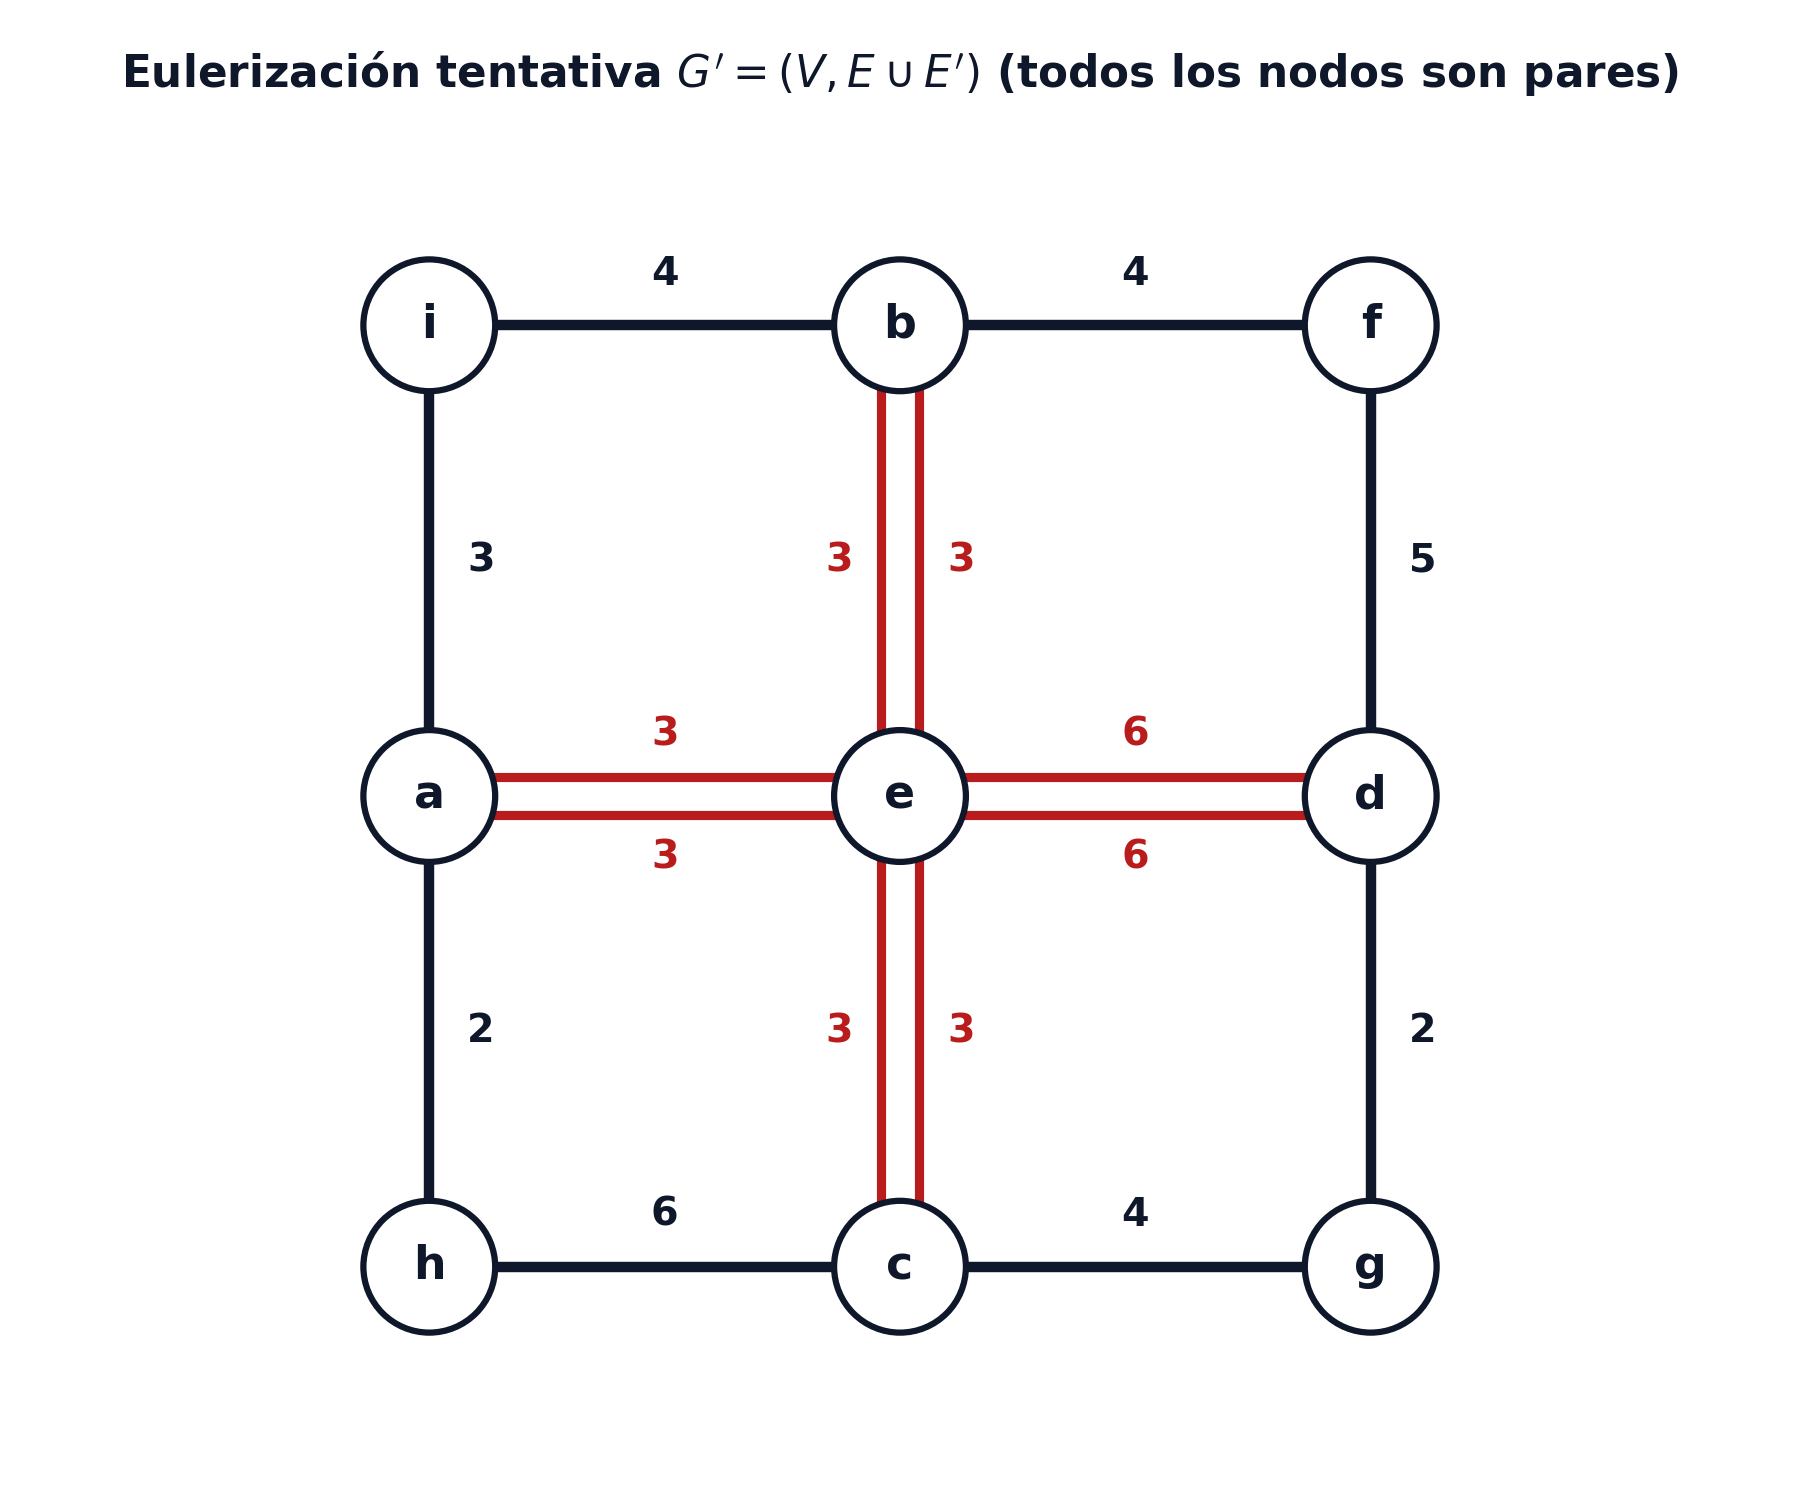
\includegraphics[width=0.6\linewidth,height=\textheight,keepaspectratio]{images/cartero_chino_eulerizacion_conceptual.png}

}

\caption{\label{fig-cartero-chino-eulerizacion-conceptual}Eulerización
conceptual tentativa de la red de 9 nodos mediante la duplicación de
aristas hacia el nodo central \(e\)}

\end{figure}%

En este multigrafo \(G'\), \textbf{todos los vértices son pares}, por lo
que ya admite un ciclo euleriano continuo. El coste añadido por esta
eulerización tentativa es: \[
\text{Coste}(E') = p(a, e) + p(b, e) + p(e, c) + p(e, d) = 3 + 3 + 3 + 6 = 15
\] Ahora bien, surge la cuestión central: \emph{¿Es este conjunto \(E'\)
el de menor coste posible, o existe otra combinación de aristas que
eulerice la red con un incremento de distancia inferior?} Para responder
a esta pregunta de forma óptima, formalizaremos a continuación la
estructura analítica del problema.

\subsection{Caracterización analítica y eulerización
óptima}\label{caracterizaciuxf3n-analuxedtica-y-eulerizaciuxf3n-uxf3ptima}

Para duplicar aristas de manera óptima, debemos formalizar la estructura
combinatoria de los vértices impares y de las aristas repetidas.

\begin{tcolorbox}[enhanced jigsaw, toprule=.15mm, opacitybacktitle=0.6, coltitle=black, colbacktitle=quarto-callout-note-color!10!white, title=\textcolor{quarto-callout-note-color}{\faInfo}\hspace{0.5em}{Proposición: Paridad del número de vértices de grado impar}, arc=.35mm, rightrule=.15mm, toptitle=1mm, breakable, bottomtitle=1mm, titlerule=0mm, colback=white, opacityback=0, leftrule=.75mm, colframe=quarto-callout-note-color-frame, left=2mm, bottomrule=.15mm]

En cualquier multigrafo finito \(G = (V, E)\), el número de vértices con
grado impar es estrictamente un \textbf{número par}.

\emph{Demostración}: Por el lema del apretón de manos (\emph{Handshaking
Lemma}), la suma de los grados de todos los vértices es igual al doble
del número de aristas: \[
\sum_{i \in V} d(i) = 2 |E|
\] Dado que \(2|E|\) es un número par, podemos descomponer la suma entre
el conjunto de vértices de grado par \(V_{\text{par}}\) y el conjunto de
vértices de grado impar \(V_{\text{impar}}\): \[
\sum_{i \in V_{\text{impar}}} d(i) + \sum_{i \in V_{\text{par}}} d(i) = 2 |E|
\] Como la suma de términos pares \(\sum_{i \in V_{\text{par}}} d(i)\)
es par, la suma \(\sum_{i \in V_{\text{impar}}} d(i)\) debe ser
obligatoriamente un número par. Puesto que la suma de una colección de
números impares es par si y solo si la cantidad de sumandos es par, se
concluye que el cardinal \(|V_{\text{impar}}|\) es necesariamente par.
\(\blacksquare\)

\end{tcolorbox}

Sea \(V' = \{v \in V \mid d(v) \equiv 1 \pmod 2\}\) el subconjunto de
vértices de grado impar en \(G\), con \(|V'| = 2k\). Para transformar
\(G\) en un multigrafo euleriano \(G' = (V, E \cup E')\), debemos añadir
un conjunto de aristas copia \(E'\) (donde cada arista de \(E'\) es un
duplicado de una arista original de \(E\)) de forma que en \(G'\) todos
los vértices tengan grado par.

\begin{tcolorbox}[enhanced jigsaw, toprule=.15mm, opacitybacktitle=0.6, coltitle=black, colbacktitle=quarto-callout-note-color!10!white, title=\textcolor{quarto-callout-note-color}{\faInfo}\hspace{0.5em}{Proposición: Estructura de caminos de las aristas duplicadas}, arc=.35mm, rightrule=.15mm, toptitle=1mm, breakable, bottomtitle=1mm, titlerule=0mm, colback=white, opacityback=0, leftrule=.75mm, colframe=quarto-callout-note-color-frame, left=2mm, bottomrule=.15mm]

Sea \(G = (V, E)\) un grafo no euleriano y sea \(E'\) un conjunto
minimal de aristas duplicadas que convierte a \(G' = (V, E \cup E')\) en
un grafo euleriano. Entonces, para todo vértice \(i_1 \in V'\), el
conjunto \(E'\) contiene una cadena que une \(i_1\) con otro vértice
\(i_2 \in V'\).

\emph{Demostración}: Por construcción, en el multigrafo eulerizado
\(G'\) se cumple que \(d_{G'}(i) \ge d_G(i)\) para todo \(i \in V\), y
todos los vértices en \(G'\) tienen grado par. Dado que \(i_1 \in V'\)
tenía grado impar en \(G\), en el grafo de aristas añadidas
\(G_{E'} = (V, E')\) el grado de \(i_1\) debe ser impar (para que la
suma \(d_G(i_1) + d_{E'}(i_1) = d_{G'}(i_1)\) sea par). Por tanto,
existe al menos una arista añadida en \(E'\) que incide en \(i_1\),
denotada por \(\{i_1, j\}\). Si el nodo \(j \in V'\), hemos encontrado
una cadena directa que une dos nodos de \(V'\) y el resultado queda
demostrado. Si \(j \notin V'\), el nodo \(j\) tenía grado par en \(G\).
Al añadir la arista \(\{i_1, j\}\), su grado en \(G'\) se volvería impar
a menos que exista otra arista \(\{j, k\} \in E'\) incidente en \(j\).
Repitiendo este razonamiento de forma secuencial sobre los nodos
intermedios, como el conjunto de vértices de la red es finito y no se
pueden generar ramas infinitas, la cadena de aristas de \(E'\) debe
terminar obligatoriamente en otro vértice \(i_2 \in V'\).
\(\blacksquare\)

\end{tcolorbox}

Esta proposición demuestra algebraicamente que \textbf{la eulerización
óptima de una red equivale a encontrar un conjunto de caminos de
longitud mínima en \(G\) que emparejen los \(2k\) vértices de grado
impar de dos en dos}. Para formalizar esta optimización combinatoria
sobre el grafo auxiliar de distancias, recordamos las definiciones
canónicas de la teoría de emparejamientos:

\begin{tcolorbox}[enhanced jigsaw, toprule=.15mm, opacitybacktitle=0.6, coltitle=black, colbacktitle=quarto-callout-note-color!10!white, title=\textcolor{quarto-callout-note-color}{\faInfo}\hspace{0.5em}{Definición: Emparejamientos y emparejamiento perfecto de peso mínimo}, arc=.35mm, rightrule=.15mm, toptitle=1mm, breakable, bottomtitle=1mm, titlerule=0mm, colback=white, opacityback=0, leftrule=.75mm, colframe=quarto-callout-note-color-frame, left=2mm, bottomrule=.15mm]

Dado un grafo no dirigido \(G = (V, E)\):

\begin{itemize}
\tightlist
\item
  \textbf{Emparejamiento (\emph{matching})}: Es un subconjunto de
  aristas \(M \subseteq E\) tales que ningún par de aristas de \(M\)
  comparte vértices en común (es decir, no existen aristas adyacentes en
  \(M\)).
\item
  \textbf{Vértice saturado}: Un vértice \(v \in V\) se dice saturado por
  \(M\) si incide en alguna arista de \(M\).
\item
  \textbf{Emparejamiento perfecto}: Un emparejamiento \(M\) es perfecto
  si \textbf{satura a todos los vértices de \(V\)} (cada nodo de \(V\)
  es extremo de exactamente una arista de \(M\)). Para que un grafo
  admita un emparejamiento perfecto, es condición necesaria que \(|V|\)
  sea par.
\item
  \textbf{Problema del emparejamiento perfecto de peso mínimo}: En una
  red valorada \(G = (V, E, p)\), consiste en determinar un
  emparejamiento perfecto \(M^*\) que minimice la suma de los pesos de
  sus aristas: \[
  \begin{aligned}
  \min_{M \subseteq E} \quad & \sum_{e \in M} p(e) \\
  \text{sujeto a} \quad & M \text{ es emparejamiento perfecto}
  \end{aligned}
  \]
\end{itemize}

\end{tcolorbox}

Dado que el grafo auxiliar \(G'' = (V', E'')\) construido sobre el
conjunto de vértices impares es completo y posee un número estrictamente
par de nodos (\(|V'| = 2k\)), siempre admite al menos un emparejamiento
perfecto. Por tanto, el procedimiento sistemático de resolución se
articula en las siguientes etapas:

\begin{tcolorbox}[enhanced jigsaw, toprule=.15mm, opacitybacktitle=0.6, coltitle=black, colbacktitle=quarto-callout-note-color!10!white, title=\textcolor{quarto-callout-note-color}{\faInfo}\hspace{0.5em}{Esquema: Procedimiento general de resolución del Problema del Cartero
Chino}, arc=.35mm, rightrule=.15mm, toptitle=1mm, breakable, bottomtitle=1mm, titlerule=0mm, colback=white, opacityback=0, leftrule=.75mm, colframe=quarto-callout-note-color-frame, left=2mm, bottomrule=.15mm]

Dado un grafo conexo valorado \(G = (V, E, p)\):

\begin{enumerate}
\def\labelenumi{\arabic{enumi}.}
\tightlist
\item
  \textbf{Identificación de vértices impares}: Determinar el grado
  \(d(i)\) de cada vértice en \(G\) e identificar el subconjunto de
  nodos impares \(V' = \{v \in V \mid d(v) \text{ es impar}\}\). Si
  \(V' = \emptyset\), el grafo es euleriano y se pasa directamente al
  paso 5.
\item
  \textbf{Cálculo de distancias mínimas}: Calcular las distancias del
  camino mínimo \(d_G(u, v)\) entre todo par de vértices \(u, v \in V'\)
  utilizando el algoritmo de Dijkstra o Floyd-Warshall.
\item
  \textbf{Construcción del grafo auxiliar de emparejamiento}: Construir
  un \textbf{grafo auxiliar completo} \(G'' = (V', E'')\), cuyos
  vértices son exclusivamente los elementos de \(V'\) y donde cada
  arista \(\{u, v\} \in E''\) tiene un peso igual a la distancia mínima
  \(d_G(u, v)\) calculada en el paso anterior.
\item
  \textbf{Resolución del emparejamiento perfecto de peso mínimo}:
  Determinar en \(G''\) un \textbf{emparejamiento perfecto de peso
  mínimo} (utilizando el algoritmo de la Flor de Edmonds o enumeración
  de combinaciones si \(|V'|\) es pequeño).
\item
  \textbf{Construcción del multigrafo euleriano y circuito final}: Para
  cada pareja de nodos \(\{u, v\}\) seleccionada en el emparejamiento
  óptimo, duplicar en \(G\) las aristas que integran el camino mínimo
  entre \(u\) y \(v\). El multigrafo resultante \(G'\) es euleriano.
  Aplicar el algoritmo de construcción euleriana para obtener la ruta
  final del cartero.
\end{enumerate}

\end{tcolorbox}

A continuación, aplicamos este procedimiento a un caso práctico de 9
nodos.

\begin{tcolorbox}[enhanced jigsaw, toprule=.15mm, opacitybacktitle=0.6, coltitle=black, colbacktitle=quarto-callout-tip-color!10!white, title=\textcolor{quarto-callout-tip-color}{\faLightbulb}\hspace{0.5em}{Ejemplo: Resolución completa del Problema del Cartero Chino en una red
de 9 nodos}, arc=.35mm, rightrule=.15mm, toptitle=1mm, breakable, bottomtitle=1mm, titlerule=0mm, colback=white, opacityback=0, leftrule=.75mm, colframe=quarto-callout-tip-color-frame, left=2mm, bottomrule=.15mm]

Consideremos la red valorada de 9 nodos
\(V = \{a, b, c, d, e, f, g, h, i\}\) y 12 aristas mostrada en la
Figura~\ref{fig-cartero-chino-grafo-original}, con los siguientes pesos
de arista: \[
\begin{aligned}
& p(i, b) = 4, \quad p(b, f) = 4, \quad p(i, a) = 3, \quad p(b, e) = 3, \quad p(f, d) = 5, \\
& p(a, e) = 3, \quad p(e, d) = 6, \quad p(a, h) = 2, \quad p(e, c) = 3, \quad p(d, g) = 2, \\
& p(h, c) = 6, \quad p(c, g) = 4
\end{aligned}
\] La suma del coste de todas las aristas originales del grafo es: \[
\sum_{e \in E} p(e) = 4 + 4 + 3 + 3 + 5 + 3 + 6 + 2 + 3 + 2 + 6 + 4 = 38
\]

\begin{figure}[H]

\centering{

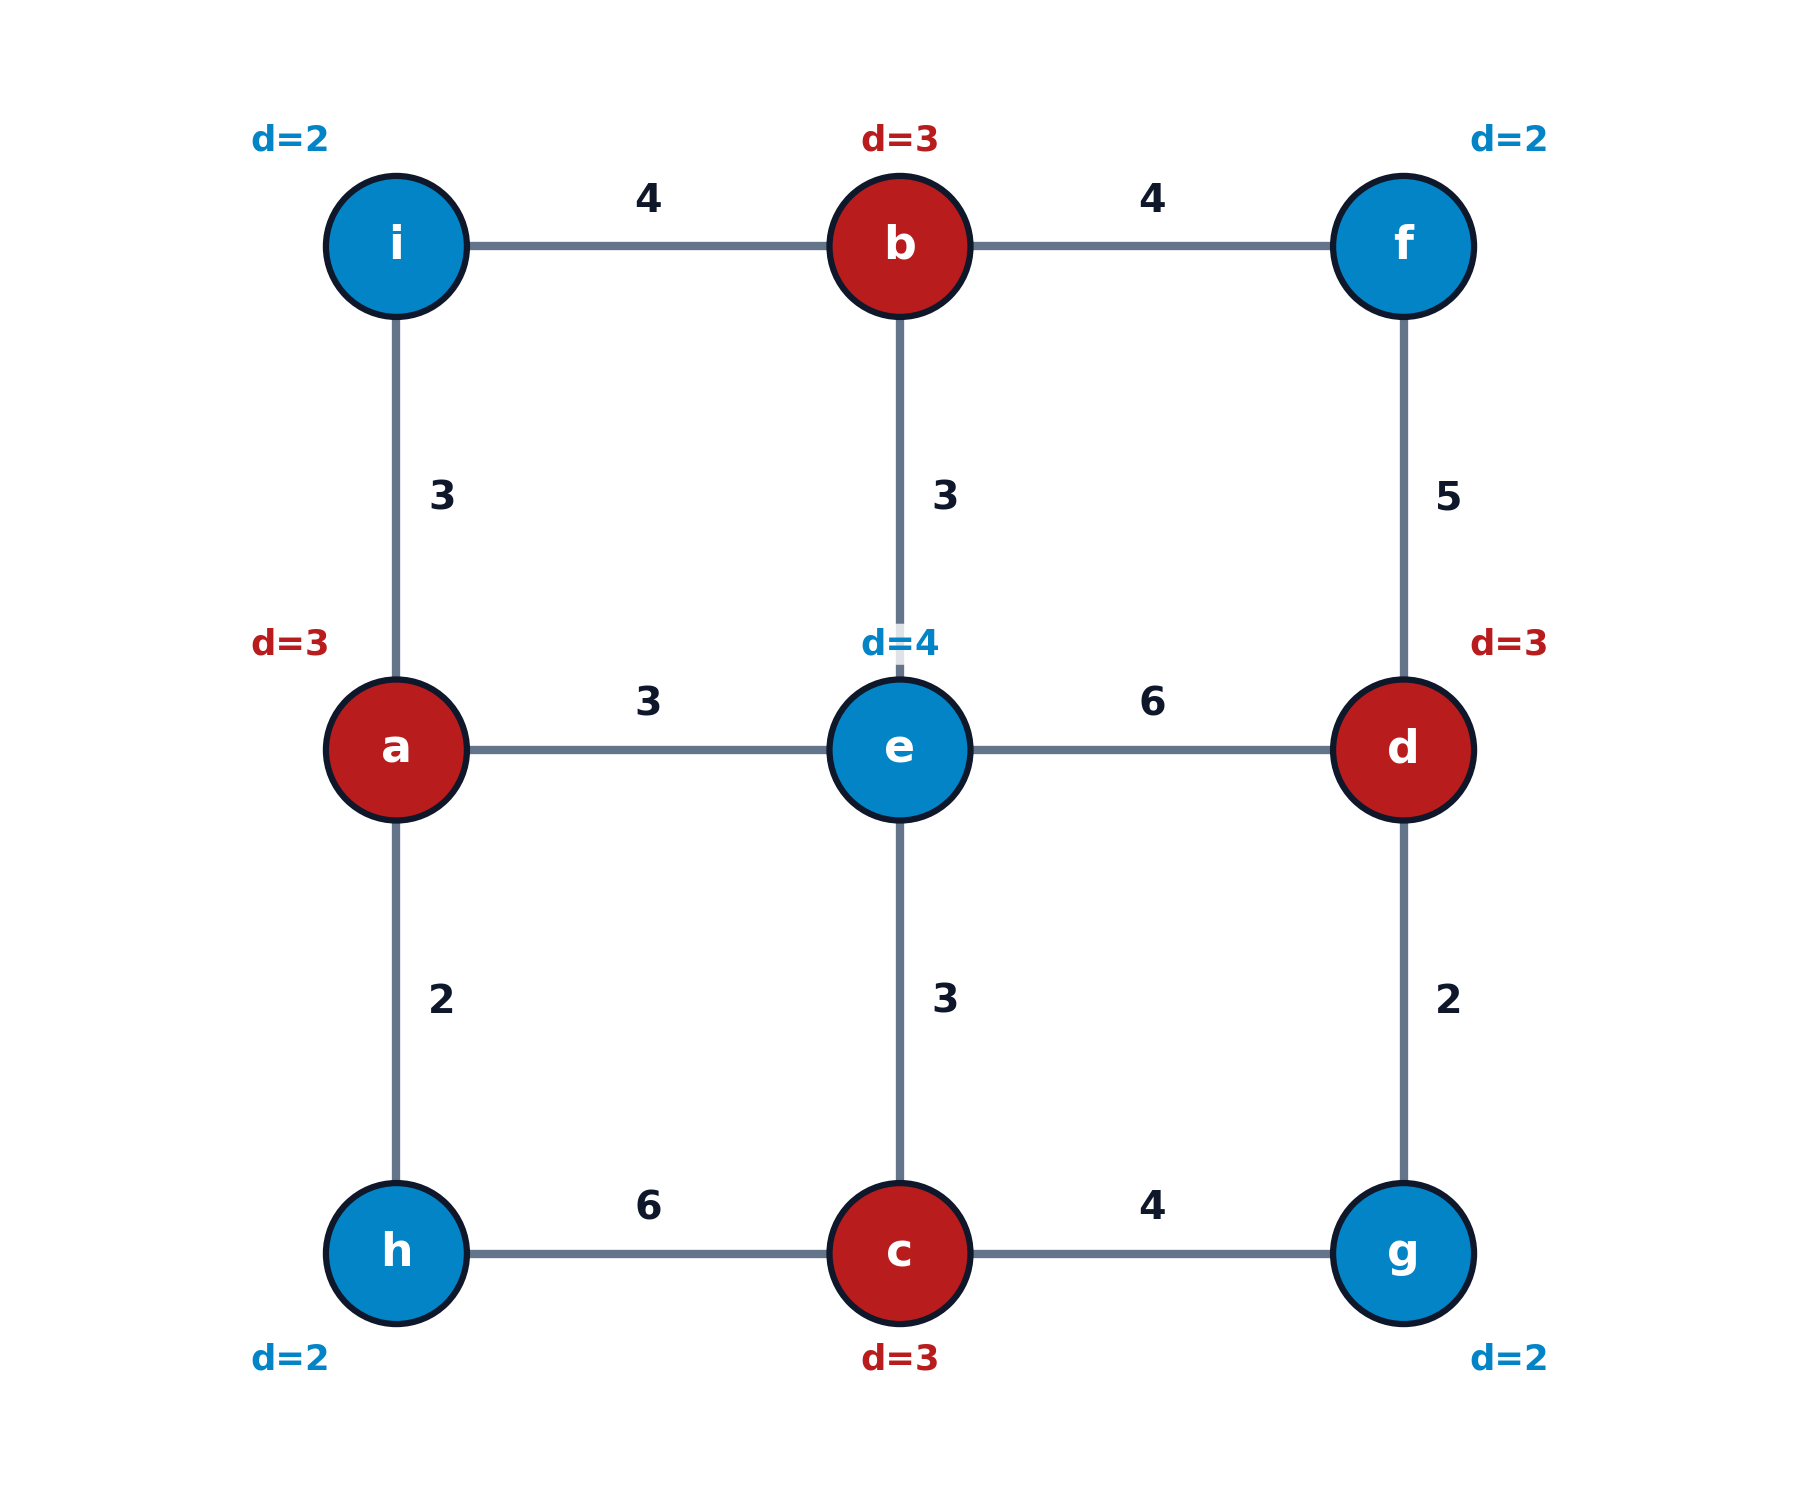
\includegraphics[width=0.6\linewidth,height=\textheight,keepaspectratio]{images/cartero_chino_grafo_original.png}

}

\caption{\label{fig-cartero-chino-grafo-original}Red valorada original
de 9 nodos para el Problema del Cartero Chino con los grados nodales y
vértices impares destacados}

\end{figure}%

\begin{enumerate}
\def\labelenumi{\arabic{enumi}.}
\item
  \textbf{Identificación de nodos impares (\(V'\))}: Calculando los
  grados de los 9 vértices: \[
  d(i)=2, \ d(b)=3, \ d(f)=2, \ d(a)=3, \ d(e)=4, \ d(d)=3, \ d(h)=2, \ d(c)=3, \ d(g)=2
  \] El subconjunto de vértices con grado impar contiene 4 nodos:
  \(V' = \{a, b, c, d\}\).
\item
  \textbf{Cálculo de caminos mínimos entre vértices de \(V'\)}:

  \begin{itemize}
  \tightlist
  \item
    Camino \(a \leftrightarrow b\): Vía \(a - e - b\), coste
    \(d(a, b) = 3 + 3 = 6\).
  \item
    Camino \(a \leftrightarrow c\): Vía \(a - e - c\), coste
    \(d(a, c) = 3 + 3 = 6\).
  \item
    Camino \(a \leftrightarrow d\): Vía \(a - e - d\), coste
    \(d(a, d) = 3 + 6 = 9\).
  \item
    Camino \(b \leftrightarrow c\): Vía \(b - e - c\), coste
    \(d(b, c) = 3 + 3 = 6\).
  \item
    Camino \(b \leftrightarrow d\): Vía \(b - f - d\), coste
    \(d(b, d) = 4 + 5 = 9\) (o vía \(b-e-d\): \(3+6=9\)).
  \item
    Camino \(c \leftrightarrow d\): Vía \(c - g - d\), coste
    \(d(c, d) = 4 + 2 = 6\).
  \end{itemize}
\item
  \textbf{Construcción de \(G''\) y evaluación de emparejamientos
  perfectos}: El grafo auxiliar completo \(G'' = (V', E'')\) sobre los 4
  nodos \(\{a, b, c, d\}\) admite exactamente tres emparejamientos
  perfectos posibles, ilustrados en la
  Figura~\ref{fig-cartero-chino-grafo-auxiliar-matching}:

  \begin{itemize}
  \item
    \textbf{Emparejamiento \(M_1 = \{ \{a, b\}, \{c, d\} \}\)}: \[
    \text{Coste}(M_1) = d(a, b) + d(c, d) = 6 + 6 = \mathbf{12} \quad \text{[ÓPTIMO]}
    \]
  \item
    \textbf{Emparejamiento \(M_2 = \{ \{a, c\}, \{b, d\} \}\)}: \[
    \text{Coste}(M_2) = d(a, c) + d(b, d) = 6 + 9 = 15
    \]
  \item
    \textbf{Emparejamiento \(M_3 = \{ \{a, d\}, \{b, c\} \}\)}: \[
    \text{Coste}(M_3) = d(a, d) + d(b, c) = 9 + 6 = 15
    \]
  \end{itemize}
\end{enumerate}

\begin{figure}[H]

\centering{

\includegraphics[width=0.9\linewidth,height=\textheight,keepaspectratio]{images/cartero_chino_grafo_auxiliar_matching.png}

}

\caption{\label{fig-cartero-chino-grafo-auxiliar-matching}Grafo auxiliar
completo \(G''\) (izquierda) y comparación de costes de los tres
emparejamientos perfectos (derecha)}

\end{figure}%

\begin{enumerate}
\def\labelenumi{\arabic{enumi}.}
\setcounter{enumi}{3}
\item
  \textbf{Eulerización y longitud óptima del circuito}: El
  emparejamiento óptimo \(M_1\) prescribe duplicar las aristas que
  componen el camino entre \(a\) y \(b\) (aristas \(\{a, e\}\) y
  \(\{e, b\}\)) y las que componen el camino entre \(c\) y \(d\)
  (aristas \(\{c, g\}\) y \(\{g, d\}\)), como se ilustra en la
  Figura~\ref{fig-cartero-chino-solucion-optima}.

  La longitud mínima de la ruta del cartero chino resulta: \[
  \text{Longitud Óptima} = \sum_{e \in E} p(e) + \text{Coste}(M_1) = 38 + 12 = \mathbf{50}
  \]
\end{enumerate}

\begin{figure}[H]

\centering{

\includegraphics[width=0.6\linewidth,height=\textheight,keepaspectratio]{images/cartero_chino_solucion_optima.png}

}

\caption{\label{fig-cartero-chino-solucion-optima}Multigrafo eulerizado
con las aristas duplicadas destacadas en rojo y la solución óptima del
cartero chino}

\end{figure}%

\end{tcolorbox}

Veamos ahora un segundo ejemplo clásico de aplicación en ingeniería
civil y delimitación de parcelas.

\begin{tcolorbox}[enhanced jigsaw, toprule=.15mm, opacitybacktitle=0.6, coltitle=black, colbacktitle=quarto-callout-tip-color!10!white, title=\textcolor{quarto-callout-tip-color}{\faLightbulb}\hspace{0.5em}{Ejemplo: Problema de examen: Vallado perimetral continuo de parcelas}, arc=.35mm, rightrule=.15mm, toptitle=1mm, breakable, bottomtitle=1mm, titlerule=0mm, colback=white, opacityback=0, leftrule=.75mm, colframe=quarto-callout-tip-color-frame, left=2mm, bottomrule=.15mm]

Se desea cercar un terreno dividiéndolo en cuatro parcelas \(A, B, C\) y
\(D\), según se indica en la Figura~\ref{fig-examen-parcelas-terreno}
(cada tramo de los bordes indica la longitud del mismo). Por motivos de
seguridad, el cerramiento se hace mediante una cerca prefabricada que se
extiende a lo largo de todos los bordes, que no se puede partir y debe
terminar exactamente donde empieza.

\begin{figure}[H]

\centering{

\includegraphics[width=0.85\linewidth,height=\textheight,keepaspectratio]{images/examen_parcelas_terreno.png}

}

\caption{\label{fig-examen-parcelas-terreno}Plano geométrico del terreno
con las cuatro parcelas A, B, C y D con sus cotas de longitud y los 6
vértices impares destacados}

\end{figure}%

\begin{enumerate}
\def\labelenumi{\arabic{enumi}.}
\item
  \textbf{(0.5 puntos) ¿Qué problema de grafos se está planteando?}: Se
  trata formalmente del \textbf{Problema del Cartero Chino (CPP)} (o
  problema de inspección de rutas). El objetivo es encontrar el circuito
  cerrado de longitud mínima que recorra todas las aristas de un grafo
  al menos una vez y regrese al punto de partida. Dado que se exige
  instalar una cerca continua que cubra todos los bordes, es necesario
  trazar un ciclo euleriano. Al contar el mapa con intersecciones donde
  confluyen tres bordes (\textbf{vértices de grado impar}), el grafo no
  es euleriano de origen. El problema consiste, por tanto, en determinar
  qué tramos deben duplicarse (para tender la cerca dos veces por el
  mismo borde) garantizando que la longitud extra sea la mínima posible.
\item
  \textbf{(1.0 punto) Describir el procedimiento de solución}: El
  procedimiento general de resolución se articula en las siguientes
  cinco etapas sistemáticas:

  \begin{itemize}
  \tightlist
  \item
    \textbf{Paso 1 (Identificación de vértices impares)}: Modelar la red
    topológica \(G = (V, E, p)\), determinar el grado \(d(v)\) de cada
    vértice e identificar el subconjunto de nodos con grado impar
    \(V' = \{v \in V \mid d(v) \equiv 1 \pmod 2\}\).
  \item
    \textbf{Paso 2 (Cálculo de distancias mínimas)}: Calcular las
    distancias del camino mínimo \(d_G(u, v)\) entre todo par de
    vértices \(u, v \in V'\) utilizando el algoritmo de Dijkstra.
  \item
    \textbf{Paso 3 (Construcción del grafo auxiliar de emparejamiento)}:
    Construir el grafo auxiliar completo \(G'' = (V', E'')\) sobre el
    conjunto de nodos impares \(V'\), asignando a cada arista
    \(\{u, v\} \in E''\) un peso igual a la distancia mínima
    \(d_G(u, v)\) calculada en el paso anterior.
  \item
    \textbf{Paso 4 (Resolución del emparejamiento perfecto de peso
    mínimo)}: Determinar en \(G''\) un \textbf{emparejamiento perfecto
    de peso mínimo} \(M^*\).
  \item
    \textbf{Paso 5 (Construcción del multigrafo euleriano y cálculo de
    la longitud final)}: Duplicar en \(G\) las aristas que integran los
    caminos mínimos asociados a cada pareja de \(M^*\). La longitud
    total de la valla continua será la suma de las longitudes de todos
    los tramos originales más el coste del emparejamiento óptimo: \[
    L_{\text{total}} = \sum_{e \in E} p(e) + \text{Coste}(M^*)
    \]
  \end{itemize}
\item
  \textbf{(1.0 punto) ¿Cuál es la solución para el caso planteado?}:
  Aplicamos de forma secuencial las 5 etapas del procedimiento descrito:

  \begin{itemize}
  \item
    \textbf{Paso 1 (Identificación de vértices impares \(V'\))}: Se
    calculan las longitudes de los tramos que delimitan el terreno:

    \begin{itemize}
    \tightlist
    \item
      \emph{Aristas internas (fronteras entre parcelas)}: Entre \(A\) y
      \(B\) (\(3\)), entre \(A\) y \(C\) (\(4\)), entre \(B\) y \(C\)
      (\(12\)), entre \(A\) y \(D\) (\(6\)), entre \(C\) y \(D\)
      (\(2 + 6 = 8\)). Suma interna = \(33\text{ m}\).
    \item
      \emph{Aristas externas (perímetro exterior)}: Borde exterior de
      \(A\) (\(2 + 9 + 1 + 2 + 4 + 2 + 4 + 5 = 29\)), borde de \(B\)
      (\(8 + 4 + 8 + 3 + 4 + 4 + 5 = 36\)), borde de \(C\)
      (\(6 + 2 + 4 + 12 = 24\)), borde de \(D\) (\(8 + 8 + 2 = 18\)).
      Suma externa = \(107\text{ m}\).
    \item
      \emph{Longitud base de la red}:
      \(L_{\text{base}} = 33 + 107 = \mathbf{140} \text{ m}\).
    \end{itemize}

    Analizando la topología, las esquinas exteriores tienen grado 2
    (par), mientras que en los 6 puntos de intersección donde confluyen
    tres lindes (puntos rojos en la
    Figura~\ref{fig-examen-parcelas-terreno}), el grado es estrictamente
    \(3\) (impar). Por tanto, el conjunto de vértices impares contiene
    \(6\) nodos: \(|V'| = 6\).
  \item
    \textbf{Paso 2 (Cálculo de distancias mínimas entre vértices de
    \(V'\))}:

    \begin{itemize}
    \tightlist
    \item
      Camino entre el punto superior (\(A\)-\(B\)) y el central
      (\(A\)-\(B\)-\(C\)): Arista interior directa con distancia
      \(d = \mathbf{3}\).
    \item
      Camino entre el punto inferior (\(A\)-\(D\)) y el central inferior
      (\(A\)-\(C\)-\(D\)): Arista interior directa con distancia
      \(d = \mathbf{6}\).
    \item
      Camino entre los dos extremos de la derecha (extremo de
      \(B\)-\(C\) y extremo de \(C\)-\(D\)): Distancia mínima
      \(d = \mathbf{24}\), alcanzable tanto por el contorno exterior de
      \(C\) (\(6 + 2 + 4 + 12 = 24\)) como por el interior
      \((B\text{-}C) + (A\text{-}C) + (C\text{-}D) = 12 + 4 + 8 = 24\).
    \end{itemize}
  \item
    \textbf{Paso 3 (Construcción del grafo auxiliar \(G''\))}: Se
    construye el grafo auxiliar completo \(G'' = (V', E'')\) sobre los 6
    vértices impares ponderado con la matriz de distancias mínimas.
  \item
    \textbf{Paso 4 (Resolución del emparejamiento perfecto de peso
    mínimo \(M^*\))}: Evaluando las combinaciones de emparejamientos
    perfectos posibles sobre los 6 vértices, el emparejamiento óptimo es
    aquel que selecciona las tres parejas mínimas identificadas: \[
    \text{Coste}(M^*) = 3 + 6 + 24 = \mathbf{33} \text{ m}
    \]
  \item
    \textbf{Paso 5 (Construcción del multigrafo euleriano y longitud
    total óptima)}: Duplicando las aristas de los caminos mínimos
    asociados a \(M^*\), todos los vértices pasan a tener grado par en
    el multigrafo resultante. La longitud mínima de la cerca
    prefabricada continua es: \[
    \begin{aligned}
    L_{\text{total}} &= L_{\text{base}} + \text{Coste}(M^*) \\
    &= 140 \text{ (base)} + 33 \text{ (duplicados)} = \mathbf{173} \text{ m}
    \end{aligned}
    \]
  \end{itemize}
\end{enumerate}

\end{tcolorbox}

\subsection{Variantes del Problema del Cartero
Chino}\label{variantes-del-problema-del-cartero-chino}

El modelo clásico no dirigido del cartero chino admite diversas
extensiones operativas de gran relevancia:

\begin{itemize}
\item
  \textbf{Cartero chino dirigido / motorizado (Directed CPP)}: En cascos
  urbanos con calles de sentido único, la red se modela como un digrafo
  \(G = (V, U)\). El digrafo es euleriano si y solo si para todo vértice
  \(i \in V\) el grado de entrada coincide con el de salida
  (\(d^-(i) = d^+(i)\)). Si la red no es euleriana, la eulerización no
  se resuelve por emparejamiento, sino mediante un \textbf{modelo de
  transbordo y flujo a coste mínimo}, donde los nodos con exceso de
  salida (\(d^+(i) > d^-(i)\)) actúan como fuentes de oferta
  \(b_i = d^+(i) - d^-(i)\) y los nodos con exceso de entrada
  (\(d^-(i) > d^+(i)\)) actúan como sumideros de demanda
  \(b_j = -(d^-(j) - d^+(j))\).
\item
  \textbf{Cartero chino con costes asimétricos / viento (Windy Postman
  Problem)}: El coste o tiempo de transitar por una calle depende de la
  dirección de avance debido a pendientes pronunciadas o corrientes de
  viento predominantes (\(c(i, j) \neq c(j, i)\)). Este problema es
  \(\mathcal{NP}\)-duro en el caso general.
\item
  \textbf{Cartero rural y problemas con beneficios y pérdidas (Rural
  Postman Problem - RPP)}: En muchas aplicaciones (como la lectura de
  contadores rurales o el mantenimiento de autopistas), solo un
  subconjunto de aristas prioritarias \(E_R \subseteq E\) debe ser
  recorrido de forma obligatoria, mientras que las restantes aristas
  \(E \setminus E_R\) pueden utilizarse libremente como vías de tránsito
  si abaratan el recorrido global. El RPP es un problema
  \(\mathcal{NP}\)-completo.
\end{itemize}

\begin{center}\rule{0.5\linewidth}{0.5pt}\end{center}

\section{Ciclos hamiltonianos y condiciones de
hamiltonianidad}\label{ciclos-hamiltonianos-y-condiciones-de-hamiltonianidad}

A diferencia de los ciclos eulerianos, cuyo objetivo es recorrer todas
las aristas de una red sin repetición, existen numerosos problemas donde
el objetivo consiste en visitar \textbf{todos los vértices} de la red
exactamente una vez.

El concepto de \textbf{ciclo hamiltoniano} debe su nombre al matemático
y astrónomo irlandés \textbf{Sir William Rowan Hamilton}, quien en 1857
patentó un juego didáctico denominado el \emph{Juego Icosiano}
(\emph{Icosian Game}) (Hamilton 1857). El pasatiempo consistía en un
tablero de madera que representaba la estructura de un dodecaedro
regular de 20 vértices (identificados con nombres de ciudades del
mundo), y el reto planteaba encontrar un recorrido a lo largo de las
aristas del poliedro que visitara las 20 ciudades exactamente una vez
sin repetir ninguna, regresando a la ciudad de origen.

\begin{tcolorbox}[enhanced jigsaw, toprule=.15mm, opacitybacktitle=0.6, coltitle=black, colbacktitle=quarto-callout-note-color!10!white, title=\textcolor{quarto-callout-note-color}{\faInfo}\hspace{0.5em}{Definición: Ciclos y caminos hamiltonianos}, arc=.35mm, rightrule=.15mm, toptitle=1mm, breakable, bottomtitle=1mm, titlerule=0mm, colback=white, opacityback=0, leftrule=.75mm, colframe=quarto-callout-note-color-frame, left=2mm, bottomrule=.15mm]

Dado un grafo \(G = (V, E)\) con \(n = |V|\) vértices:

\begin{itemize}
\tightlist
\item
  \textbf{Ciclo hamiltoniano}: Es un ciclo simple en \(G\) que contiene
  \textbf{todos los vértices de \(V\)} exactamente una vez (excepto el
  vértice de partida, al que regresa para cerrar el ciclo).
\item
  \textbf{Camino hamiltoniano}: Es una trayectoria o camino simple en
  \(G\) que visita todos los vértices de \(V\) exactamente una vez (sin
  regresar al origen).
\item
  \textbf{Grafo hamiltoniano}: Un grafo que admite al menos un ciclo
  hamiltoniano.
\end{itemize}

\end{tcolorbox}

A pesar de la aparente similitud conceptual entre el problema euleriano
(visitar todas las aristas) y el problema hamiltoniano (visitar todos
los vértices), existe un abismo infranqueable en su \textbf{complejidad
computacional}:

\begin{itemize}
\tightlist
\item
  El problema de determinar si un grafo es euleriano se resuelve de
  forma instantánea en tiempo lineal \(\mathcal{O}(|V| + |E|)\)
  comprobando la paridad de los grados. Pertenece a la clase
  \(\mathcal{P}\).
\item
  El problema de determinar si un grafo general contiene un ciclo
  hamiltoniano (\textbf{HAMILTONIAN-CYCLE}) es uno de los 21 problemas
  clásicos demostrados como \textbf{\(\mathcal{NP}\)-completos} por
  Richard Karp en 1972 (Karp 1972).
\end{itemize}

No se conocen condiciones necesarias y suficientes simultáneamente que
puedan verificarse en tiempo polinomial. Por ello, el análisis formal se
apoya en condiciones necesarias de corte y condiciones suficientes
basadas en la densidad de grados.

\subsection{Condiciones necesarias: 2-conexidad y cortes
nodales}\label{condiciones-necesarias-2-conexidad-y-cortes-nodales}

Para que un grafo admita un ciclo hamiltoniano, debe poseer una
estructura de conectividad robusta que garantice la existencia de rutas
alternativas.

\begin{tcolorbox}[enhanced jigsaw, toprule=.15mm, opacitybacktitle=0.6, coltitle=black, colbacktitle=quarto-callout-note-color!10!white, title=\textcolor{quarto-callout-note-color}{\faInfo}\hspace{0.5em}{Definición: Conjuntos de corte y k-conexidad}, arc=.35mm, rightrule=.15mm, toptitle=1mm, breakable, bottomtitle=1mm, titlerule=0mm, colback=white, opacityback=0, leftrule=.75mm, colframe=quarto-callout-note-color-frame, left=2mm, bottomrule=.15mm]

Dado un grafo conexo \(G = (V, E)\):

\begin{itemize}
\tightlist
\item
  \textbf{Conjunto de corte de vértices}: Un subconjunto de vértices
  \(A \subset V\) es un conjunto de corte si el subgrafo inducido por
  los restantes vértices \(V \setminus A\) es disconexo.
\item
  \textbf{Grafo \(k\)-conexo}: Un grafo \(G\) es \(k\)-conexo si
  \(|V| \ge k+1\) y no contiene ningún conjunto de corte de cardinal
  menor que \(k\) (es decir, se requiere eliminar al menos \(k\)
  vértices para desconectar el grafo). En particular, todo grafo
  \(k\)-conexo satisface \(d_G(i) \ge k\) para todo \(i \in V\).
\end{itemize}

\end{tcolorbox}

\begin{tcolorbox}[enhanced jigsaw, toprule=.15mm, opacitybacktitle=0.6, coltitle=black, colbacktitle=quarto-callout-note-color!10!white, title=\textcolor{quarto-callout-note-color}{\faInfo}\hspace{0.5em}{Proposición: Condición necesaria de 2-conexidad}, arc=.35mm, rightrule=.15mm, toptitle=1mm, breakable, bottomtitle=1mm, titlerule=0mm, colback=white, opacityback=0, leftrule=.75mm, colframe=quarto-callout-note-color-frame, left=2mm, bottomrule=.15mm]

Si un grafo \(G = (V, E)\) es hamiltoniano, entonces \(G\) es
obligatoriamente \textbf{2-conexo} (no posee vértices de corte o puntos
de articulación).

\emph{Demostración}: Demostremos el resultado por reducción al absurdo.
Supongamos que \(G\) es hamiltoniano pero no es 2-conexo. Entonces,
existe un conjunto de corte \(A = \{v\}\) formado por un único vértice
(punto de articulación), cuya eliminación divide al grafo en al menos
dos componentes conexas disyuntas \(G_1\) y \(G_2\). Cualquier ciclo
hamiltoniano \(C\) debe visitar la totalidad de los vértices de \(G_1\)
y de \(G_2\). Para transitar desde los vértices de \(G_1\) hacia los de
\(G_2\), el ciclo debe pasar obligatoriamente por el único vértice
conector \(v\). Asimismo, para regresar de \(G_2\) a \(G_1\) y poder
cerrar el ciclo, el recorrido debe transitar una segunda vez por \(v\).
Por tanto, el ciclo pasaría al menos dos veces por \(v\), contradiciendo
la definición de ciclo simple hamiltoniano. \(\blacksquare\)

\end{tcolorbox}

La 2-conexidad es una condición estrictamente \textbf{necesaria pero no
suficiente}. En la Figura~\ref{fig-hamilton-2conexo-contraejemplo} se
muestra un contraejemplo clásico: un grafo de 5 nodos formado por tres
caminos paralelos entre los nodos \(a\) y \(e\). El grafo es 2-conexo
(no se desconecta eliminando un solo nodo y todos sus vértices cumplen
\(d(v) \ge 2\)), pero no es hamiltoniano porque cualquier ciclo que
visite \(b, c\) y \(d\) (que tienen grado 2) requeriría pasar tres veces
por \(a\) y por \(e\).

\begin{figure}

\centering{

\includegraphics[width=0.5\linewidth,height=\textheight,keepaspectratio]{images/hamilton_2conexo_contraejemplo.png}

}

\caption{\label{fig-hamilton-2conexo-contraejemplo}Contraejemplo: grafo
2-conexo que no es hamiltoniano debido al estrangulamiento en los nodos
conectores}

\end{figure}%

\subsection{Condiciones suficientes: Proposición de adyacencia y Teorema
de Bondy y
Chvátal}\label{condiciones-suficientes-proposiciuxf3n-de-adyacencia-y-teorema-de-bondy-y-chvuxe1tal}

Para establecer condiciones suficientes de hamiltonianidad, se estudian
los grafos completos y el efecto de añadir aristas entre vértices de
grado elevado.

\begin{tcolorbox}[enhanced jigsaw, toprule=.15mm, opacitybacktitle=0.6, coltitle=black, colbacktitle=quarto-callout-note-color!10!white, title=\textcolor{quarto-callout-note-color}{\faInfo}\hspace{0.5em}{Proposición: Hamiltonianidad del grafo completo}, arc=.35mm, rightrule=.15mm, toptitle=1mm, breakable, bottomtitle=1mm, titlerule=0mm, colback=white, opacityback=0, leftrule=.75mm, colframe=quarto-callout-note-color-frame, left=2mm, bottomrule=.15mm]

Todo grafo simple completo \(K_n\) con \(n \ge 3\) vértices es
hamiltoniano y contiene exactamente: \[
\frac{(n-1)!}{2}
\] ciclos hamiltonianos distintos no orientados (\(n!\) si se considera
el orden y sentido de recorrido).

\end{tcolorbox}

El resultado teórico fundamental que sustenta las condiciones modernas
de suficiencia establece que añadir una arista entre dos nodos cuya suma
de grados supera el número total de vértices no altera la condición de
hamiltonianidad del grafo.

\begin{tcolorbox}[enhanced jigsaw, toprule=.15mm, opacitybacktitle=0.6, coltitle=black, colbacktitle=quarto-callout-important-color!10!white, title=\textcolor{quarto-callout-important-color}{\faExclamation}\hspace{0.5em}{Teorema: Proposición fundamental de adyacencia de Bondy y Chvátal}, arc=.35mm, rightrule=.15mm, toptitle=1mm, breakable, bottomtitle=1mm, titlerule=0mm, colback=white, opacityback=0, leftrule=.75mm, colframe=quarto-callout-important-color-frame, left=2mm, bottomrule=.15mm]

Sea \(G = (V, E)\) un grafo simple con \(n = |V| \ge 3\) vértices y sean
\(s, t \in V\) dos vértices \textbf{no adyacentes} tales que la suma de
sus grados cumple: \[
d_G(s) + d_G(t) \ge n
\] Se define el grafo ampliado
\(G + \{s, t\} = (V, E \cup \{\{s, t\}\})\). Entonces: \[
G \text{ es hamiltoniano} \iff G + \{s, t\} \text{ es hamiltoniano}
\]

\emph{Demostración}: La implicación directa (\(\implies\)) es trivial:
si \(G\) ya contiene un ciclo hamiltoniano, dicho ciclo existe
igualmente en el supergrafo \(G + \{s, t\}\).

Demostremos la implicación recíproca (\(\impliedby\)). Supongamos que
\(G + \{s, t\}\) contiene un ciclo hamiltoniano \(C\). Si la arista
añadida \(\{s, t\}\) no forma parte de \(C\), entonces \(C\) está
contenido íntegramente en \(G\) y el resultado queda demostrado.
Supongamos ahora que \(\{s, t\} \in C\). Numeramos los vértices a lo
largo del ciclo \(C\) comenzando en \(s = x_1\) y terminando en
\(t = x_n\), de modo que el ciclo en \(G + \{s, t\}\) es: \[
s = x_1 \to x_2 \to x_3 \to \dots \to x_{n-1} \to x_n = t \xrightarrow{\{s, t\}} s
\] Para reconstruir un ciclo hamiltoniano en el grafo original \(G\) sin
utilizar la arista \(\{s, t\}\), buscamos un índice intermedio
\(i \in \{2, 3, \dots, n-2\}\) tal que en \(G\) existan simultáneamente
la arista \(\{s, x_{i+1}\}\) y la arista \(\{t, x_i\}\), como se ilustra
en la Figura~\ref{fig-hamilton-adyacencia-demostracion}.

Definimos los siguientes dos subconjuntos de vértices: \[
\begin{aligned}
A &= \{ x_i \in V \mid \{s, x_{i+1}\} \in E, \ i \in \{2, \dots, n-2\} \} \\
B &= \{ x_i \in V \mid \{t, x_i\} \in E, \ i \in \{2, \dots, n-2\} \}
\end{aligned}
\] Evaluemos los cardinales de estos conjuntos:

\begin{itemize}
\tightlist
\item
  El vértice \(s\) puede ser adyacente a lo sumo a los nodos
  \(\{x_2, \dots, x_{n-1}\}\). Dado que \(\{s, t\} \notin E\) y
  descontando la arista \(\{s, x_2\}\) (cuyo predecesor es \(x_1\)), el
  número de vecinos de \(s\) entre los nodos \(\{x_3, \dots, x_{n-1}\}\)
  es \(|A| = d_G(s) - 1\).
\item
  De igual forma, el vértice \(t\) no está conectado a \(s\), y
  descontando su conexión con \(x_{n-1}\), se tiene
  \(|B| = d_G(t) - 1\).
\end{itemize}

Sumando ambos cardinales: \[
|A| + |B| = (d_G(s) - 1) + (d_G(t) - 1) = d_G(s) + d_G(t) - 2 \ge n - 2
\] Por otra parte, ambos conjuntos están contenidos en el universo
\(U = \{x_2, x_3, \dots, x_{n-2}\}\), cuyo cardinal es \(|U| = n - 3\).
Por tanto, la unión satisface \(|A \cup B| \le n - 3\). Aplicando el
principio de inclusión-exclusión: \[
|A \cap B| = |A| + |B| - |A \cup B| \ge (n - 2) - (n - 3) = 1
\] Como \(|A \cap B| \ge 1\), la intersección es \textbf{no vacía}
(\(A \cap B \neq \emptyset\)). Existe al menos un vértice \(x_i\) tal
que \(\{s, x_{i+1}\} \in E\) y \(\{t, x_i\} \in E\).

Eliminando del ciclo \(C\) las aristas \(\{s, t\}\) y
\(\{x_i, x_{i+1}\}\) e insertando las aristas \(\{s, x_{i+1}\}\) y
\(\{t, x_i\}\), se obtiene el ciclo: \[
s \to x_2 \to \dots \to x_i \to t \to x_{n-1} \to x_{n-2} \to \dots \to x_{i+1} \to s
\] Este ciclo recorre todos los vértices de \(V\) una sola vez y está
compuesto exclusivamente por aristas de \(E\). Por tanto, \(G\) es
hamiltoniano. \(\blacksquare\)

\begin{figure}[H]

\centering{

\includegraphics[width=0.75\linewidth,height=\textheight,keepaspectratio]{images/hamilton_adyacencia_demostracion.png}

}

\caption{\label{fig-hamilton-adyacencia-demostracion}Esquema
demostrativo de la proposición de adyacencia: sustitución de aristas
para reconstruir el ciclo hamiltoniano}

\end{figure}%

\end{tcolorbox}

La aplicación iterativa de esta proposición conduce de forma natural al
concepto de \textbf{clausura}.

\begin{tcolorbox}[enhanced jigsaw, toprule=.15mm, opacitybacktitle=0.6, coltitle=black, colbacktitle=quarto-callout-note-color!10!white, title=\textcolor{quarto-callout-note-color}{\faInfo}\hspace{0.5em}{Definición: Clausura de Bondy y Chvátal}, arc=.35mm, rightrule=.15mm, toptitle=1mm, breakable, bottomtitle=1mm, titlerule=0mm, colback=white, opacityback=0, leftrule=.75mm, colframe=quarto-callout-note-color-frame, left=2mm, bottomrule=.15mm]

Dado un grafo simple \(G = (V, E)\) con \(n\) vértices, la
\textbf{clausura de \(G\)}, denotada por \([G]\), es el grafo obtenido
añadiendo recursivamente aristas entre parejas de vértices no adyacentes
\(u, v\) que satisfacen \(d(u) + d(v) \ge n\), hasta que no sea posible
añadir ninguna arista adicional. La clausura \([G]\) es única e
independiente del orden en que se añadan las aristas.

\end{tcolorbox}

\begin{tcolorbox}[enhanced jigsaw, toprule=.15mm, opacitybacktitle=0.6, coltitle=black, colbacktitle=quarto-callout-important-color!10!white, title=\textcolor{quarto-callout-important-color}{\faExclamation}\hspace{0.5em}{Teorema: Teorema de Bondy y Chvátal (1976)}, arc=.35mm, rightrule=.15mm, toptitle=1mm, breakable, bottomtitle=1mm, titlerule=0mm, colback=white, opacityback=0, leftrule=.75mm, colframe=quarto-callout-important-color-frame, left=2mm, bottomrule=.15mm]

Un grafo simple \(G\) es \textbf{hamiltoniano si y solo si su clausura
\([G]\) es hamiltoniana}. En particular, si la clausura de \(G\) es el
grafo completo (\([G] = K_n\)), entonces \(G\) es \textbf{hamiltoniano}
(Bondy y Chvátal 1976).

\end{tcolorbox}

La caracterización de Bondy y Chvátal establece una equivalencia lógica
exacta (\(G\) hamiltoniano \(\iff [G]\) hamiltoniano). No obstante,
cuando se utiliza la condición simplificada de clausura completa
\([G] = K_n\) como criterio práctico de verificación, debe tenerse en
cuenta su naturaleza asimétrica:

\begin{tcolorbox}[enhanced jigsaw, toprule=.15mm, opacitybacktitle=0.6, coltitle=black, colbacktitle=quarto-callout-warning-color!10!white, title=\textcolor{quarto-callout-warning-color}{\faExclamationTriangle}\hspace{0.5em}{Advertencia: El criterio \([G] = K_n\) es condición suficiente, pero no
necesaria}, arc=.35mm, rightrule=.15mm, toptitle=1mm, breakable, bottomtitle=1mm, titlerule=0mm, colback=white, opacityback=0, leftrule=.75mm, colframe=quarto-callout-warning-color-frame, left=2mm, bottomrule=.15mm]

Es crucial resaltar que la condición de que la clausura alcance el grafo
completo (\([G] = K_n\)) es una \textbf{condición suficiente pero no
necesaria} para la existencia de ciclos hamiltonianos.

Como contraejemplo fundamental, consideremos el \textbf{grafo ciclo}
\(C_5 = (a, b, d, e, c, a)\) de \(n=5\) vértices ilustrado en la
Figura~\ref{fig-hamilton-clausura-contraejemplo-c5}. Este grafo es
\textbf{evidentemente hamiltoniano} (el propio ciclo recorre todos sus
vértices una sola vez). Sin embargo, al ser un ciclo simple regular de
grado 2, todos sus vértices satisfacen \(d(v) = 2\). Por tanto, para
cualquier par de vértices no adyacentes \(u, v\), la suma de grados
resulta: \[
d(u) + d(v) = 2 + 2 = 4 < n = 5
\] Al no cumplirse la condición en ningún par, no es posible añadir
ninguna arista, por lo que la clausura coincide con el grafo original:
\([C_5] = C_5 \neq K_5\). Por consiguiente, si la clausura de un grafo
no es completa (\([G] \neq K_n\)), \textbf{no se puede deducir que el
grafo no sea hamiltoniano} (el criterio de clausura completa resulta no
concluyente).

\begin{figure}[H]

\centering{

\includegraphics[width=0.6\linewidth,height=\textheight,keepaspectratio]{images/hamilton_clausura_contraejemplo_c5.png}

}

\caption{\label{fig-hamilton-clausura-contraejemplo-c5}Contraejemplo de
suficiencia: el grafo ciclo \(C_5\) es hamiltoniano pero su clausura no
es el grafo completo}

\end{figure}%

\end{tcolorbox}

Como corolarios directos del teorema de Bondy y Chvátal se deducen de
forma inmediata los teoremas clásicos de suficiencia más célebres de la
literatura:

\begin{tcolorbox}[enhanced jigsaw, toprule=.15mm, opacitybacktitle=0.6, coltitle=black, colbacktitle=quarto-callout-note-color!10!white, title=\textcolor{quarto-callout-note-color}{\faInfo}\hspace{0.5em}{Corolario: Teoremas clásicos de Dirac (1952) y Ore (1960)}, arc=.35mm, rightrule=.15mm, toptitle=1mm, breakable, bottomtitle=1mm, titlerule=0mm, colback=white, opacityback=0, leftrule=.75mm, colframe=quarto-callout-note-color-frame, left=2mm, bottomrule=.15mm]

Sea \(G = (V, E)\) un grafo simple con \(n \ge 3\) vértices:

\begin{itemize}
\tightlist
\item
  \textbf{Teorema de Ore (1960)}: Si para todo par de vértices no
  adyacentes \(u, v \in V\) se cumple \(d(u) + d(v) \ge n\), entonces
  \(G\) es hamiltoniano (su clausura es directamente el grafo completo
  \(K_n\)).
\item
  \textbf{Teorema de Dirac (1952)}: Si el grado mínimo de todo vértice
  cumple \(d(v) \ge \frac{n}{2}\) para todo \(v \in V\), entonces para
  cualquier par no adyacente
  \(d(u) + d(v) \ge \frac{n}{2} + \frac{n}{2} = n\), y por tanto \(G\)
  es hamiltoniano (Dirac 1952; Ore 1960).
\end{itemize}

\end{tcolorbox}

En el siguiente ejemplo, ilustramos el cálculo de la clausura en dos
grafos distintos.

\begin{tcolorbox}[enhanced jigsaw, toprule=.15mm, opacitybacktitle=0.6, coltitle=black, colbacktitle=quarto-callout-tip-color!10!white, title=\textcolor{quarto-callout-tip-color}{\faLightbulb}\hspace{0.5em}{Ejemplo: Cálculo y evaluación de la clausura de Bondy y Chvátal}, arc=.35mm, rightrule=.15mm, toptitle=1mm, breakable, bottomtitle=1mm, titlerule=0mm, colback=white, opacityback=0, leftrule=.75mm, colframe=quarto-callout-tip-color-frame, left=2mm, bottomrule=.15mm]

Analicemos los dos grafos representados en la
Figura~\ref{fig-bondy-chvatal-ejemplos}:

\begin{enumerate}
\def\labelenumi{\arabic{enumi}.}
\tightlist
\item
  \textbf{Ejemplo 1 (Grafo de 4 nodos, panel izquierdo)}:

  \begin{itemize}
  \tightlist
  \item
    Vértices: \(V = \{a, b, c, d\}\), con \(n = 4\).
  \item
    Aristas originales:
    \(\{a, b\}, \{a, c\}, \{a, d\}, \{b, c\}, \{b, d\}\).
  \item
    Grados iniciales: \(d(a)=3, d(b)=3, d(c)=2, d(d)=2\).
  \item
    El único par de vértices no adyacentes es \(\{c, d\}\).
  \item
    Evaluando la condición: \(d(c) + d(d) = 2 + 2 = 4 \ge n = 4\).
  \item
    Se añade la arista \(\{c, d\}\). El grafo resultante es el grafo
    completo \(K_4\).
  \item
    Por el Teorema de Bondy y Chvátal, \([G] = K_4 \implies G\)
    \textbf{es hamiltoniano}.
  \end{itemize}
\item
  \textbf{Ejemplo 2 (Grafo de 5 nodos, panel derecho)}:

  \begin{itemize}
  \tightlist
  \item
    Vértices: \(V = \{a, b, c, d, e\}\), con \(n = 5\).
  \item
    Aristas iniciales:
    \(\{a, b\}, \{b, e\}, \{a, c\}, \{c, e\}, \{a, d\}, \{d, e\}\).
  \item
    Grados iniciales: \(d(a)=3, d(e)=3, d(b)=2, d(c)=2, d(d)=2\).
  \item
    Evaluando pares no adyacentes:

    \begin{itemize}
    \tightlist
    \item
      Para \(\{a, e\}\): \(d(a) + d(e) = 3 + 3 = 6 \ge 5\). Se añade la
      arista \(\{a, e\}\).
    \item
      Los grados se actualizan a \(d(a)=4, d(e)=4\).
    \item
      Evaluando los restantes pares no adyacentes
      \(\{b, c\}, \{c, d\}, \{b, d\}\): \(d(b) + d(c) = 2 + 2 = 4 < 5\),
      \(d(c) + d(d) = 4 < 5\), \(d(b) + d(d) = 4 < 5\).
    \end{itemize}
  \item
    No es posible añadir más aristas. La clausura \([G]\) no es completa
    (\([G] \neq K_5\)). La condición de suficiencia no permite
    certificar la hamiltonianidad (el grafo no es hamiltoniano).
  \end{itemize}
\end{enumerate}

\begin{figure}[H]

\centering{

\includegraphics[width=0.9\linewidth,height=\textheight,keepaspectratio]{images/bondy_chvatal_ejemplos.png}

}

\caption{\label{fig-bondy-chvatal-ejemplos}Cálculo de la clausura de
Bondy y Chvátal: clausura completa \([G]=K_4\) (izquierda) y clausura
incompleta (derecha)}

\end{figure}%

\end{tcolorbox}

\begin{center}\rule{0.5\linewidth}{0.5pt}\end{center}

\section{El Problema del Viajante de Comercio
(TSP)}\label{el-problema-del-viajante-de-comercio-tsp}

El \textbf{Problema del Viajante de Comercio} (conocido mundialmente
como \emph{Traveling Salesperson Problem}, TSP) es, sin lugar a dudas,
el problema más emblemático, estudiado y emblemático de la optimización
combinatoria y la programación entera (G. Dantzig, Fulkerson, y Johnson
1954; Applegate et~al. 2006).

El problema modela la situación de un agente comercial que debe partir
de una ciudad base, visitar un conjunto de \(n\) ciudades exactamente
una vez y regresar al punto de partida, de modo que la
\textbf{distancia, tiempo o coste económico total acumulado sea mínimo}.

Las aplicaciones reales del TSP trascienden con creces el ruteo físico
de personas y vehículos. Entre sus aplicaciones industriales más
destacadas figuran:

\begin{itemize}
\tightlist
\item
  \textbf{Fabricación de circuitos impresos (PCB drilling)}:
  Optimización del orden de perforación de decenas de miles de orificios
  en placas electrónicas mediante brazos robóticos láser para minimizar
  el tiempo de desplazamiento del cabezal.
\item
  \textbf{Secuenciación de tareas en máquinas (Sequence-dependent
  scheduling)}: Programación de lotes de producción en una máquina
  industrial donde el tiempo de limpieza y ajuste entre tareas depende
  de la tarea inmediatamente precedente (tiempos de cambio de matriz en
  prensas o purga de color en pintura).
\item
  \textbf{Astronomía y observación espacial}: Secuenciación óptima de
  apuntado de telescopios orbitales (como el Hubble o James Webb) entre
  constelaciones celestes para minimizar el consumo de combustible en
  maniobras giroscópicas.
\item
  \textbf{Biología computacional y genómica}: Reconstrucción y
  alineamiento de secuencias de fragmentos de ADN en el ensamblaje de
  genomas.
\end{itemize}

\begin{tcolorbox}[enhanced jigsaw, toprule=.15mm, opacitybacktitle=0.6, coltitle=black, colbacktitle=quarto-callout-note-color!10!white, title=\textcolor{quarto-callout-note-color}{\faInfo}\hspace{0.5em}{Definición: Problema del Viajante de Comercio (TSP)}, arc=.35mm, rightrule=.15mm, toptitle=1mm, breakable, bottomtitle=1mm, titlerule=0mm, colback=white, opacityback=0, leftrule=.75mm, colframe=quarto-callout-note-color-frame, left=2mm, bottomrule=.15mm]

Dado un conjunto de \(n\) ciudades \(V = \{1, 2, \dots, n\}\) y una
matriz de costes o distancias \(D = (d_{ij})_{n \times n}\), donde
\(d_{ij} \ge 0\) representa el coste de desplazarse directamente desde
la ciudad \(i\) hasta la ciudad \(j\):

El \textbf{TSP} consiste en encontrar una permutación
\(\pi = (\pi(1), \pi(2), \dots, \pi(n))\) de las \(n\) ciudades que
minimice el coste total del ciclo hamiltoniano: \[
\min_{\pi} \left( \sum_{k=1}^{n-1} d_{\pi(k), \pi(k+1)} + d_{\pi(n), \pi(1)} \right)
\]

\end{tcolorbox}

Para abordar el TSP mediante optimizadores matemáticos (\emph{solvers}
de programación lineal entera), se han desarrollado diversas
formulaciones con propiedades teóricas y computacionales muy dispares.
Analizaremos las tres formulaciones fundamentales: el modelo por etapas
o tramos (\(x_{ijk}\)), el modelo clásico de eliminación exponencial de
subciclos de Dantzig, Fulkerson y Johnson (DFJ), y la formulación
compacta polinomial de Miller, Tucker y Zemlin (MTZ).

\subsection{\texorpdfstring{Modelo 1 del TSP: Variables de posición de
tramo
(\(x_{ijk}\))}{Modelo 1 del TSP: Variables de posición de tramo (x\_\{ijk\})}}\label{modelo-1-del-tsp-variables-de-posiciuxf3n-de-tramo-x_ijk}

Una primera aproximación intuitiva para modelar el TSP mediante
Programación Lineal Entera consiste en concebir el itinerario del agente
como una secuencia ordenada de \(n\) etapas o tramos temporales
sucesivos.

\textbf{Variables de decisión}: Para formular este modelo, se introducen
las variables binarias con triple subíndice \(x_{ijk} \in \{0, 1\}\),
definidas como: \[
x_{ijk} = \begin{cases} 
1 & \text{si el agente se desplaza directamente de } i \text{ a } j \text{ en la etapa } k \\ 
0 & \text{en otro caso} 
\end{cases}
\] para todo \(i, j, k \in \{1, \dots, n\}\).

\textbf{Construcción pedagógica de las restricciones}: A partir de estas
variables, la exigencia de que la solución forme un ciclo hamiltoniano
válido y continuo se traduce en cinco condiciones estructurales
fundamentales:

\begin{enumerate}
\def\labelenumi{\arabic{enumi}.}
\item
  \textbf{Minimización de la distancia total (Función objetivo)}: Cada
  desplazamiento entre \(i\) y \(j\) devenga un coste \(d_{ij}\)
  independientemente de la etapa \(k\) en la que se realice. La
  distancia total acumulada a lo largo de las \(n\) etapas del viaje es:
  \[
  \min_{x} \sum_{i=1}^n \sum_{j=1}^n \sum_{k=1}^n d_{ij} x_{ijk}
  \]
\item
  \textbf{Salida única de cada ciudad}: El agente debe abandonar cada
  ciudad \(i\) exactamente una vez a lo largo del viaje completo,
  dirigiéndose hacia alguna ciudad \(j\) en alguna de las \(n\) etapas
  \(k\): \[
  \sum_{j=1}^n \sum_{k=1}^n x_{ijk} = 1, \quad \forall i = 1, \dots, n
  \]
\item
  \textbf{Llegada única a cada ciudad}: El agente debe acceder a cada
  ciudad \(j\) exactamente una vez a lo largo del viaje completo,
  proviniendo de alguna ciudad \(i\) en alguna etapa \(k\): \[
  \sum_{i=1}^n \sum_{k=1}^n x_{ijk} = 1, \quad \forall j = 1, \dots, n
  \]
\item
  \textbf{Ocupación exclusiva de cada etapa temporal}: En cada etapa
  \(k \in \{1, \dots, n\}\) del itinerario solo puede llevarse a cabo
  exactamente un trayecto entre un par de ciudades: \[
  \sum_{i=1}^n \sum_{j=1}^n x_{ijk} = 1, \quad \forall k = 1, \dots, n
  \]
\item
  \textbf{Continuidad espacial del recorrido entre etapas consecutivas}:
  Si en la etapa \(k\) el agente llega a la ciudad \(j\) (sumando sobre
  todos los posibles orígenes \(i \neq j\)), en la siguiente etapa
  \(k+1\) debe partir obligatoriamente desde esa misma ciudad \(j\)
  (sumando sobre todos los posibles destinos \(l \neq j\)): \[
  \sum_{i \neq j} x_{ijk} = \sum_{l \neq j} x_{j,l,k+1}, \quad \forall j = 1, \dots, n, \quad \forall k = 1, \dots, n
  \] Para la última etapa \(k = n\), la etapa subsiguiente \(k+1\) se
  identifica circularmente con la etapa inicial \(1\).
\end{enumerate}

\textbf{Formulación matemática consolidada del Modelo 1}: Reuniendo
todas las condiciones analizadas, el modelo completo de programación
lineal entera queda formulado de la siguiente manera: \[
\begin{aligned}
\min_{x} \quad & \sum_{i=1}^n \sum_{j=1}^n \sum_{k=1}^n d_{ij} x_{ijk} \\
\text{sujeto a} \quad & \sum_{j=1}^n \sum_{k=1}^n x_{ijk} = 1, \quad \forall i = 1, \dots, n \\
& \sum_{i=1}^n \sum_{k=1}^n x_{ijk} = 1, \quad \forall j = 1, \dots, n \\
& \sum_{i=1}^n \sum_{j=1}^n x_{ijk} = 1, \quad \forall k = 1, \dots, n \\
& \sum_{i \neq j} x_{ijk} = \sum_{l \neq j} x_{j,l,k+1}, \quad \forall j = 1, \dots, n, \ k = 1, \dots, n \\
& x_{ijk} \in \{0, 1\}, \quad \forall i, j, k = 1, \dots, n
\end{aligned}
\]

Desde el punto de vista computacional, este modelo requiere \(n^3\)
variables binarias y \(3n + n^2\) restricciones para una red de \(n\)
ciudades. Aunque su planteamiento resulta transparente e intuitivo, el
crecimiento cúbico de las variables limita su aplicación práctica a
problemas de escala reducida.

\subsection{Modelo 2 del TSP: Eliminación exponencial de subciclos
(DFJ)}\label{modelo-2-del-tsp-eliminaciuxf3n-exponencial-de-subciclos-dfj}

Para reducir drásticamente el número de variables de decisión, George
Dantzig, Delbert Fulkerson y Selmer Johnson propusieron en 1954
prescindir del subíndice temporal \(k\) y trabajar exclusivamente con
variables de arco (G. Dantzig, Fulkerson, y Johnson 1954).

\textbf{Variables de decisión y grado de asignación}: En este enfoque,
la elección de las rutas se describe mediante variables binarias con
doble subíndice: \[
x_{ij} = \begin{cases} 
1 & \text{si el arco dirigido } (i, j) \text{ forma parte de la ruta} \\ 
0 & \text{en otro caso} 
\end{cases}
\] para todo \(i, j \in \{1, \dots, n\}\) con \(i \neq j\).

Si imponemos únicamente las restricciones clásicas del problema de
asignación:

\begin{itemize}
\tightlist
\item
  \textbf{Conservación de salida (Grado exterior 1)}:
  \(\sum_{j=1, j \neq i}^n x_{ij} = 1, \quad \forall i = 1, \dots, n\)
\item
  \textbf{Conservación de entrada (Grado interior 1)}:
  \(\sum_{i=1, i \neq j}^n x_{ij} = 1, \quad \forall j = 1, \dots, n\)
\end{itemize}

cada ciudad tiene garantizado un único predecesor y un único sucesor.
Sin embargo, estas dos condiciones no garantizan la conectividad global,
permitiendo que la solución óptima se fracture en múltiples subciclos
desconectados (\emph{subtours}), como se ilustra en la
Figura~\ref{fig-tsp-subtours-asignacion}.

\begin{figure}

\centering{

\includegraphics[width=0.75\linewidth,height=\textheight,keepaspectratio]{images/tsp_subtours_asignacion.png}

}

\caption{\label{fig-tsp-subtours-asignacion}Fenómeno de subciclos
desconectados generado por la relajación de asignación pura en una red
de 7 nodos}

\end{figure}%

\textbf{Restricciones de eliminación de subciclos (SEC)}: Para erradicar
cualquier subciclo aislado, Dantzig, Fulkerson y Johnson establecieron
que para todo subconjunto propio no vacío de ciudades \(S \subset V\)
con cardinal \(2 \le |S| \le n-1\), el número de arcos dirigidos cuyos
dos extremos pertenezcan a \(S\) no puede alcanzar el valor \(|S|\), ya
que ello formaría un ciclo cerrado aislado dentro de \(S\). Esta
condición da lugar a las \textbf{restricciones de eliminación de
subciclos} (SEC): \[
\sum_{i \in S} \sum_{j \in S} x_{ij} \le |S| - 1, \quad \forall S \subset V, \ 2 \le |S| \le n-1
\]

\textbf{Formulación matemática consolidada del Modelo DFJ}: Integrando
la función objetivo, las restricciones de grado y las restricciones SEC,
la formulación clásica DFJ se consolida como: \[
\begin{aligned}
\min_{x} \quad & \sum_{i=1}^n \sum_{j=1}^n d_{ij} x_{ij} \\
\text{sujeto a} \quad & \sum_{j=1, j \neq i}^n x_{ij} = 1, \quad \forall i = 1, \dots, n \\
& \sum_{i=1, i \neq j}^n x_{ij} = 1, \quad \forall j = 1, \dots, n \\
& \sum_{i \in S} \sum_{j \in S} x_{ij} \le |S| - 1, \quad \forall S \subset V, \ 2 \le |S| \le n-1 \\
& x_{ij} \in \{0, 1\}, \quad \forall i, j = 1, \dots, n, \ i \neq j
\end{aligned}
\]

Aunque el modelo DFJ requiere únicamente \(n(n-1)\) variables binarias,
el número de restricciones SEC es de orden exponencial (\(2^n - 2\)). No
obstante, este modelo posee la relajación lineal continua más ajustada y
fuerte conocida en optimización combinatoria. En la práctica, los
algoritmos modernos de ramificación y corte (\emph{Branch-and-Cut})
resuelven instancias de decenas de miles de ciudades incorporando las
restricciones SEC de forma perezosa y dinámica (\emph{lazy constraints})
únicamente cuando se detecta un subciclo violado.

\subsection{Modelo 3 del TSP: Formulación compacta MTZ
(Miller-Tucker-Zemlin)}\label{modelo-3-del-tsp-formulaciuxf3n-compacta-mtz-miller-tucker-zemlin}

En 1960, Clair Miller, Albert Tucker y Richard Zemlin desarrollaron una
formulación alternativa que elimina los subciclos utilizando un número
estrictamente polinomial de restricciones (\(\mathcal{O}(n^2)\)),
permitiendo introducir el modelo completo directamente en cualquier
optimizador lineal estándar sin necesidad de generadores de cortes
dinámicos (Miller, Tucker, y Zemlin 1960).

\textbf{Variables continuas de orden secuencial}: El modelo MTZ toma una
ciudad de referencia como depósito base (fijando habitualmente
\(u_1 = 1\)) y define variables continuas auxiliares \(u_i \ge 0\) para
\(i = 2, \dots, n\), las cuales representan la posición o número de
orden en el que la ciudad \(i\) es visitada a lo largo del recorrido
(satisfaciendo \(2 \le u_i \le n\)).

\textbf{Mecánica algebraica de las restricciones MTZ}: La eliminación de
subciclos se consigue imponiendo la siguiente familia de inecuaciones
cuadráticas en el número de nodos: \[
u_i - u_j + n x_{ij} \le n - 1, \quad \forall i, j \in \{2, \dots, n\}, \ i \neq j
\]

Para comprender el fundamento algebraico de esta inecuación, analizamos
los dos valores posibles de la variable binaria \(x_{ij}\):

\begin{enumerate}
\def\labelenumi{\arabic{enumi}.}
\item
  \textbf{Si el arco \((i, j)\) forma parte de la ruta
  (\(x_{ij} = 1\))}: Sustituyendo \(x_{ij} = 1\) en la inecuación se
  obtiene \(u_i - u_j + n(1) \le n - 1 \iff u_j \ge u_i + 1\). La
  restricción fuerza de manera estricta a que el orden de visita de la
  ciudad \(j\) sea al menos una unidad mayor que el orden de la ciudad
  \(i\). Como los índices deben crecer estrictamente a lo largo de
  cualquier subrecorrido, es imposible formar un subciclo cerrado que no
  contenga al depósito 1 (pues un subciclo
  \(i_1 \to i_2 \to \dots \to i_m \to i_1\) exigiría
  \(u_{i_1} < u_{i_2} < \dots < u_{i_m} < u_{i_1}\), lo cual constituye
  una imposibilidad matemática).
\item
  \textbf{Si el arco \((i, j)\) no se utiliza (\(x_{ij} = 0\))}:
  Sustituyendo \(x_{ij} = 0\), la inecuación queda
  \(u_i - u_j + 0 \le n - 1 \iff u_i - u_j \le n - 1\). Dado que las
  variables de orden satisfacen \(2 \le u_i \le n\), la máxima
  diferencia posible entre dos índices cualesquiera es
  \((n) - (2) = n - 2 \le n - 1\). Por consiguiente, la restricción
  queda completamente desactivada y resulta redundante, no imponiendo
  ninguna limitación artificial sobre nodos no conectados.
\end{enumerate}

\textbf{Formulación matemática consolidada del Modelo MTZ}: El modelo
compacto MTZ se consolida formalmente como: \[
\begin{aligned}
\min_{x, u} \quad & \sum_{i=1}^n \sum_{j=1}^n d_{ij} x_{ij} \\
\text{sujeto a} \quad & \sum_{j=1, j \neq i}^n x_{ij} = 1, \quad \forall i = 1, \dots, n \\
& \sum_{i=1, i \neq j}^n x_{ij} = 1, \quad \forall j = 1, \dots, n \\
& u_i - u_j + n x_{ij} \le n - 1, \quad \forall i, j \in \{2, \dots, n\}, \ i \neq j \\
& u_i \ge 0, \quad \forall i = 2, \dots, n \\
& x_{ij} \in \{0, 1\}, \quad \forall i, j = 1, \dots, n, \ i \neq j
\end{aligned}
\]

En la comparativa entre MTZ y DFJ destacan dos factores determinantes:

\begin{itemize}
\tightlist
\item
  \textbf{Ventaja de MTZ}: Es un modelo compacto con \(n^2 + n - 1\)
  variables y \(n^2 - n + 2\) restricciones, resoluble directamente por
  cualquier \emph{solver} estándar sin rutinas auxiliares de separación
  de cortes.
\item
  \textbf{Desventaja de MTZ}: Su relajación lineal continua es
  significativamente más débil que la de DFJ, lo que provoca que los
  algoritmos de ramificación y acotación (\emph{Branch-and-Bound})
  requieran explorar un árbol de búsqueda mucho mayor para instancias
  medianas o grandes.
\end{itemize}

\subsection{Heurísticas y el Algoritmo de Aproximación de
Christofides}\label{heuruxedsticas-y-el-algoritmo-de-aproximaciuxf3n-de-christofides}

Dada la complejidad \(\mathcal{NP}\)-dura del TSP, en problemas de gran
tamaño se recurre a heurísticas y algoritmos de aproximación con
garantías teóricas:

\begin{itemize}
\tightlist
\item
  \textbf{Heurística constructiva del Vecino más Cercano (Nearest
  Neighbor)}: Parte de un nodo inicial y en cada paso salta al nodo no
  visitado más cercano en tiempo \(\mathcal{O}(n^2)\). Aunque es muy
  rápida, suele dejar nodos aislados lejanos para el final, generando un
  retorno final de coste elevado.
\item
  \textbf{Heurística de mejora local 2-Opt}: Parte de una ruta inicial
  válida y evalúa parejas de aristas \(\{ (u, v), (x, y) \}\). Si
  sustituirlas por \(\{ (u, x), (v, y) \}\) reduce la distancia total
  (lo que equivale a invertir el sentido de recorrido del subsegmento
  intermedio), se aplica el intercambio. Se itera hasta alcanzar un
  óptimo local 2-óptimo.
\end{itemize}

Para el \textbf{TSP métrico} (donde las distancias satisfacen la
desigualdad triangular \(d_{ij} \le d_{ik} + d_{kj}\)), el matemático
greco-británico \textbf{Nicos Christofides} desarrolló en 1976 un
célebre algoritmo de aproximación polinomial (Christofides 1976).

\begin{tcolorbox}[enhanced jigsaw, toprule=.15mm, opacitybacktitle=0.6, coltitle=black, colbacktitle=quarto-callout-note-color!10!white, title=\textcolor{quarto-callout-note-color}{\faInfo}\hspace{0.5em}{Esquema: Algoritmo de aproximación de Christofides (1976)}, arc=.35mm, rightrule=.15mm, toptitle=1mm, breakable, bottomtitle=1mm, titlerule=0mm, colback=white, opacityback=0, leftrule=.75mm, colframe=quarto-callout-note-color-frame, left=2mm, bottomrule=.15mm]

Dado un grafo completo con distancias no negativas que satisfacen la
desigualdad triangular:

\begin{enumerate}
\def\labelenumi{\arabic{enumi}.}
\tightlist
\item
  \textbf{Árbol Soporte de Mínimo Peso (MST)}: Calcular un árbol
  generador de mínimo peso \(T\) sobre el conjunto de nodos \(V\)
  mediante el algoritmo de Kruskal o Prim.
\item
  \textbf{Identificación de vértices impares}: Identificar el
  subconjunto \(O \subset V\) de vértices que tienen grado impar en el
  árbol \(T\) (el número \(|O|\) es necesariamente par).
\item
  \textbf{Emparejamiento perfecto de peso mínimo}: Calcular el
  emparejamiento perfecto de peso mínimo \(M\) sobre el subgrafo
  inducido por los vértices de \(O\) en el grafo original.
\item
  \textbf{Construcción del multigrafo euleriano}: Unir las aristas del
  árbol \(T\) y las del emparejamiento \(M\) para formar el multigrafo
  \(H = T \cup M\). En \(H\), todos los vértices tienen grado par.
\item
  \textbf{Ciclo euleriano y atajos hamiltonianos}: Hallar un ciclo
  euleriano en \(H\) y transformarlo en un ciclo hamiltoniano
  recorriendo sus vértices y aplicando \textbf{atajos}
  (\emph{shortcuts}), es decir, saltando directamente a nodos no
  visitados omitiendo nodos repetidos.
\end{enumerate}

\end{tcolorbox}

\begin{figure}

\centering{

\includegraphics[width=0.95\linewidth,height=\textheight,keepaspectratio]{images/christofides_pasos_esquema.png}

}

\caption{\label{fig-christofides-pasos-esquema}Las cuatro fases del
Algoritmo de Christofides: (1) MST, (2) Emparejamiento en impares, (3)
Multigrafo euleriano y (4) Atajos hamiltonianos}

\end{figure}%

\begin{tcolorbox}[enhanced jigsaw, toprule=.15mm, opacitybacktitle=0.6, coltitle=black, colbacktitle=quarto-callout-important-color!10!white, title=\textcolor{quarto-callout-important-color}{\faExclamation}\hspace{0.5em}{Teorema: Garantía de aproximación de factor 1.5 de Christofides}, arc=.35mm, rightrule=.15mm, toptitle=1mm, breakable, bottomtitle=1mm, titlerule=0mm, colback=white, opacityback=0, leftrule=.75mm, colframe=quarto-callout-important-color-frame, left=2mm, bottomrule=.15mm]

En cualquier grafo métrico, el algoritmo de Christofides garantiza una
solución cuyo coste no supera \textbf{1.5 veces el coste de la solución
óptima global}: \[
\text{Coste}(C_{\text{Christofides}}) \le \frac{3}{2} \text{Coste}(C^*)
\]

\emph{Demostración}: Sea \(C^*\) el ciclo hamiltoniano óptimo global del
TSP.

\begin{enumerate}
\def\labelenumi{\arabic{enumi}.}
\item
  \textbf{Cota del MST}: Si eliminamos una arista arbitraria del ciclo
  óptimo \(C^*\), obtenemos un camino simple que conecta todos los
  vértices. Dado que cualquier camino generador es un árbol soporte, y
  el MST \(T\) es por definición el árbol generador de menor peso: \[
  \text{Coste}(T) \le \text{Coste}(\text{camino}) < \text{Coste}(C^*)
  \]
\item
  \textbf{Cota del Emparejamiento}: Consideremos el ciclo óptimo \(C^*\)
  proyectado únicamente sobre el subconjunto de nodos impares \(O\),
  omitiendo mediante atajos los nodos que no pertenecen a \(O\). Por la
  desigualdad triangular, el coste de este ciclo inducido \(C^*_O\)
  cumple \(\text{Coste}(C^*_O) \le \text{Coste}(C^*)\). Al tener \(|O|\)
  un número par de vértices, el ciclo \(C^*_O\) puede descomponerse en
  dos emparejamientos perfectos disjuntos y alternos \(M_1\) y \(M_2\).
  La suma de sus costes satisface: \[
  \text{Coste}(M_1) + \text{Coste}(M_2) = \text{Coste}(C^*_O) \le \text{Coste}(C^*)
  \] Como \(M\) es el emparejamiento perfecto de peso mínimo sobre
  \(O\): \[
  \text{Coste}(M) \le \min \{ \text{Coste}(M_1), \text{Coste}(M_2) \} \le \frac{1}{2} \text{Coste}(C^*)
  \]
\item
  \textbf{Combinación y atajos}: Sumando las aristas del multigrafo
  euleriano \(H = T \cup M\): \[
  \begin{aligned}
  \text{Coste}(H) &= \text{Coste}(T) + \text{Coste}(M) \\
  &< \text{Coste}(C^*) + \frac{1}{2} \text{Coste}(C^*) = \frac{3}{2} \text{Coste}(C^*)
  \end{aligned}
  \] Al aplicar atajos para convertir el recorrido euleriano en el ciclo
  hamiltoniano \(C\), la desigualdad triangular garantiza que el coste
  no aumenta:
  \(\text{Coste}(C) \le \text{Coste}(H) \le 1.5 \text{Coste}(C^*)\).
  \(\blacksquare\)
\end{enumerate}

\end{tcolorbox}

\begin{center}\rule{0.5\linewidth}{0.5pt}\end{center}

\section{Taxonomía y características de los Problemas de Rutas de
Vehículos
(VRP)}\label{taxonomuxeda-y-caracteruxedsticas-de-los-problemas-de-rutas-de-vehuxedculos-vrp}

Tanto el Problema del Viajante de Comercio (TSP) como el Problema del
Cartero Chino (CPP) constituyen los bloques fundacionales de una
disciplina de extraordinaria amplitud en la ingeniería de sistemas, la
investigación operativa y la logística de distribución: la familia de
los \textbf{Problemas de Rutas de Vehículos} (\emph{Vehicle Routing
Problems}, VRP), introducidos formalmente por George Dantzig y John
Ramser en 1959 (G. B. Dantzig y Ramser 1959).

Mientras que el TSP tradicional asume un único agente con capacidad
infinita que visita un conjunto cerrado de ciudades, los problemas de
distribución industrial involucran flotas heterogéneas, restricciones de
capacidad volumétrica o de tonelaje, ventanas temporales estrictas de
entrega y múltiples centros logísticos de origen y destino.

Desde la perspectiva topológica, la primera distinción conceptual básica
radica en la localización espacial de las demandas que deben ser
atendidas dentro de la infraestructura de transporte, dando lugar a dos
grandes familias complementarias esquematizadas en la
Figura~\ref{fig-vrp-taxonomia-topologica}:

\begin{itemize}
\tightlist
\item
  \textbf{Problemas de rutas por nodos (Node Routing)}: Los puntos de
  demanda o clientes se sitúan exclusivamente en los \textbf{vértices}
  de la red, mientras que las aristas actúan únicamente como vías
  transitables de desplazamiento. Esta categoría engloba desde el TSP
  elemental hasta el \textbf{Problema de Rutas de Vehículos con
  Capacidad} (\emph{Capacitated VRP}, CVRP) (donde una flota de
  vehículos con capacidad limitada \(Q\) abastece a múltiples clientes
  partiendo de un depósito), el \textbf{VRP con Ventanas de Tiempo}
  (VRPTW) y los problemas de \textbf{recogida y entrega simultánea}
  (\emph{Pickup and Delivery Problem}, PDP).
\item
  \textbf{Problemas de rutas por arcos (Arc Routing)}: Las demandas o
  servicios se encuentran distribuidos de manera continua a lo largo de
  las \textbf{aristas o arcos} de la red viaria. Mientras que el
  \textbf{Problema del Cartero Chino (CPP)} exige transitar por todas
  las aristas de la red (inspección de tuberías, líneas eléctricas o
  pavimentos), el \textbf{Problema del Cartero Rural (RPP)} atiende
  únicamente a un subconjunto prioritario de tramos. Cuando se
  consideran flotas con capacidad de carga finita, se formula el
  \textbf{Problema de Rutas por Arcos con Capacidad} (CARP), estándar en
  la recogida municipal de residuos sólidos urbanos y el esparcimiento
  de sal en vialidad invernal.
\item
  \textbf{Problemas de rutas mixtos (General Routing Problems - GRP)}:
  Combinan servicios puntuales concentrados en ciertos vértices con
  demandas continuas distribuidas a lo largo de aristas específicas de
  la red.
\end{itemize}

\begin{figure}

\centering{

\includegraphics[width=0.85\linewidth,height=\textheight,keepaspectratio]{images/vrp_taxonomia_topologica.png}

}

\caption{\label{fig-vrp-taxonomia-topologica}Taxonomía topológica de
problemas de rutas: bifurcación entre rutas por arcos (Arc Routing) y
rutas por nodos (Node Routing)}

\end{figure}%

Por otra parte, la traslación de estos problemas a modelos matemáticos
computables y aplicables a la logística real requiere caracterizar con
precisión seis dimensiones operativas fundamentales, ilustradas en la
Figura~\ref{fig-vrp-dimensiones-operativas}:

\begin{itemize}
\tightlist
\item
  \textbf{Composición y capacidad de la flota}: Se distingue entre
  \emph{flotas homogéneas}, donde todos los vehículos son idénticos en
  capacidad de carga, autonomía y costes operativos, y \emph{flotas
  heterogéneas}, donde coexisten vehículos de diversas tipologías con
  posibles restricciones de gálibo o acceso físico a cascos urbanos
  históricos.
\item
  \textbf{Topología de las instalaciones y depósitos}: En los esquemas
  \emph{monodepósito}, todos los vehículos inician y concluyen su
  recorrido en una base central única. En los esquemas
  \emph{multidepósito} (\emph{Multi-Depot VRP}), la distribución se
  coordina desde múltiples centros territoriales, pudiendo los vehículos
  pernoctar en su base de origen o admitir reubicación libre entre
  depósitos.
\item
  \textbf{Certidumbre y dinamismo de la demanda}: Frente a los modelos
  \emph{deterministas}, donde las cantidades requeridas por cada cliente
  se conocen con exactitud antes de iniciar las expediciones, los
  entornos \emph{estocásticos o dinámicos} modelan la demanda como
  variables aleatorias o procesan solicitudes de última hora recibidas
  telemáticamente durante la ejecución en curso de la ruta.
\item
  \textbf{Modalidad de las operaciones de transporte}: Comprende desde
  la \emph{entrega pura} (el vehículo parte cargado y se vacía
  progresivamente) y la \emph{recogida pura} (el vehículo parte vacío y
  va acumulando mercancía o residuos) hasta las \emph{operaciones
  combinadas de recogida y entrega simultánea}, que exigen monitorizar
  la capacidad residual disponible en cada tramo intermedio de la ruta.
\item
  \textbf{Restricciones temporales y ventanas de servicio}: Varían desde
  horizontes abiertos sin limitaciones horarias hasta \emph{ventanas de
  tiempo rígidas} (\emph{Hard Time Windows}), donde el servicio fuera
  del intervalo \([a_i, b_i]\) está estrictamente prohibido, o
  \emph{ventanas flexibles} (\emph{Soft Time Windows}), donde los
  adelantos o retrasos se penalizan económicamente en la función
  objetivo.
\item
  \textbf{Estructura de costes y objetivos de optimización}: Aunque el
  objetivo clásico consiste en minimizar la distancia total recorrida,
  el tiempo de conducción o el consumo de combustible, los modelos
  avanzados integran la minimización del número total de vehículos
  activos, la reducción de emisiones de \(\text{CO}_2\) y el
  \emph{equilibrio de las cargas de trabajo} (\emph{fair workload
  balancing}) entre los conductores.
\end{itemize}

\begin{figure}

\centering{

\includegraphics[width=0.9\linewidth,height=\textheight,keepaspectratio]{images/vrp_dimensiones_operativas.png}

}

\caption{\label{fig-vrp-dimensiones-operativas}Ejes y dimensiones
fundamentales de clasificación operativa en la logística de rutas de
vehículos}

\end{figure}%

\bookmarksetup{startatroot}

\chapter*{Conclusiones}\label{sec-conclusiones}
\addcontentsline{toc}{chapter}{Conclusiones}

\markboth{Conclusiones}{Conclusiones}

A lo largo de diez capítulos estructurados en dos grandes bloques
temáticos, hemos presentado el material de la asignatura de
\textbf{Optimización y Análisis de Redes} del Grado en
\textbf{Matemáticas}.

En este capítulo de cierre, te invitamos a reflexionar sobre las
principales lecciones aprendidas durante el curso, destacando cómo el
rigor matemático y el pensamiento analítico se convierten en
herramientas indispensables para dominar la modelización matemática.
Además, animamos a los estudiantes a continuar explorando y ampliando
sus conocimientos en cursos posteriores, consolidando una base sólida
para afrontar los desafíos de la optimización y la ciencia de datos
moderna desde una perspectiva analítica, rigurosa y fundamentada.

Al finalizar este recorrido, queda patente que la optimización es mucho
más que una colección de algoritmos aislados, constituyendo un marco de
pensamiento estructurado para tomar decisiones óptimas bajo condiciones
de recursos limitados. Hemos transitado desde los fundamentos continuos
del análisis convexo y las condiciones de optimalidad hasta la
estructura discreta y combinatorial de las redes y grafos, equipando a
los futuros matemáticos con herramientas capaces de modelar, resolver e
interpretar problemas complejos del mundo real.

\section*{Resumen del aprendizaje}\label{resumen-del-aprendizaje}
\addcontentsline{toc}{section}{Resumen del aprendizaje}

\markright{Resumen del aprendizaje}

A lo largo de este manual, hemos construido un conocimiento progresivo y
bidireccional sobre la optimización matemática, cubriendo los siguientes
pilares:

\begin{enumerate}
\def\labelenumi{\arabic{enumi}.}
\item
  \textbf{Fundamentos y ciclo de la Investigación Operativa (Tema 1)}:
  Partimos de las raíces históricas y metodológicas de la disciplina,
  analizando las fases del ciclo de vida de un modelo matemático y
  formalizando la estructura canónica de los problemas de optimización
  con variables, función objetivo y restricciones.
\item
  \textbf{Optimización no lineal continua y métodos numéricos (Tema 2)}:
  Analizamos algoritmos univariantes sin derivadas (búsqueda dicotómica,
  sección áurea, Fibonacci) y con derivadas (bisección, Newton), así
  como métodos multivariantes directos (coordenadas cíclicas,
  Hooke-Jeeves), de primer orden (máximo descenso de Cauchy) y de
  segundo orden (Newton multivariante y Cuasi-Newton BFGS).
\item
  \textbf{Análisis convexo y subgradientes (Tema 3)}: Establecimos el
  marco teórico que garantiza la globalidad de los óptimos mediante
  conjuntos convexos, hiperplanos de separación y de soporte, y
  funciones convexas caracterizadas por gradientes y matrices hessianas,
  introduciendo el subgradiente y el subdiferencial para el tratamiento
  de funciones no diferenciables.
\item
  \textbf{Condiciones de optimalidad KKT, dualidad y Programación
  Cuadrática (Temas 4 y 5)}: Dedujimos las condiciones necesarias de
  Fritz-John y las condiciones necesarias y suficientes de
  Karush-Kuhn-Tucker (KKT) bajo cualificación de restricciones (LICQ y
  Slater). Aplicamos este formalismo a la Programación Lineal
  (demostrando la equivalencia con las variables duales del Símplex) y a
  la Programación Cuadrática mediante el método del Símplex de Wolfe con
  regla de entrada restringida.
\item
  \textbf{Estructuras de redes, Total Unimodularidad, árboles y caminos
  mínimos (Temas 6 y 7)}: Pasamos al dominio discreto de los grafos.
  Analizamos la propiedad de Total Unimodularidad (TUM) de la matriz de
  incidencia nodo-arco como puente que preserva la integridad en
  relajaciones continuas. Estudiamos árboles soporte de mínimo peso
  (Prim y Kruskal) y algoritmos de camino óptimo (Dijkstra,
  Bellman-Ford, Floyd-Warshall) junto con su formulación dual mediante
  potenciales nodales y tensiones.
\item
  \textbf{Flujos en redes, emparejamientos y problemas de rutas
  eulerianas, hamiltonianas y VRP (Temas 8, 9 y 10)}: Abordamos
  problemas combinatorios avanzados: el teorema de Flujo Máximo - Corte
  Mínimo de Ford-Fulkerson y Edmonds-Karp, el flujo de coste mínimo,
  emparejamientos y asignación óptima (Teoremas de Hall y Kőnig,
  Algoritmo Húngaro y Blossom de Edmonds), circuitos eulerianos (Cartero
  Chino), ciclos hamiltonianos, formulaciones de Programación Lineal
  Entera del TSP (modelos por etapas, DFJ con cortes de subciclo y MTZ
  compacto), aproximación de Christofides y la taxonomía del VRP.
\end{enumerate}

\section*{Reflexiones finales}\label{reflexiones-finales}
\addcontentsline{toc}{section}{Reflexiones finales}

\markright{Reflexiones finales}

El estudio de la \textbf{Optimización y el Análisis de Redes} dota al
matemático de un puente directo entre la abstracción algebraica y
analítica y la resolución de problemas tangibles de toma de decisiones.
Hemos visto cómo conceptos teóricos profundos (como la geometría
convexa, la dualidad lineal y la estructura combinatorial de grafos) se
traducen en algoritmos computacionales de alta eficiencia que gestionan
la logística, las finanzas o las telecomunicaciones modernas.

Hemos aprendido que modelar no es un proceso mecánico ni una mera
aplicación de recetas informáticas. Construir un modelo útil requiere un
proceso iterativo de \textbf{abstracción, resolución, validación y
análisis de sensibilidad}. Entender las hipótesis que garantizan la
convergencia de un algoritmo o la integridad de una solución es lo que
distingue a un matemático de un aplicador de software a ciegas.

\section*{Proyección futura: El valor del rigor
matemático}\label{proyecciuxf3n-futura-el-valor-del-rigor-matemuxe1tico}
\addcontentsline{toc}{section}{Proyección futura: El valor del rigor
matemático}

\markright{Proyección futura: El valor del rigor matemático}

Las competencias adquiridas en esta asignatura son esenciales en el
perfil del matemático moderno. Vuestra formación os proporciona una
ventaja competitiva fundamental: la capacidad de ir más allá del código,
comprendiendo la geometría del espacio factible, la estabilidad de las
restricciones y la justificación teórica de los óptimos obtenidos.

Este conocimiento es el lenguaje compartido con la \textbf{Investigación
Operativa} avanzada, el \textbf{Aprendizaje Automático} y la
\textbf{Ciencia de Datos Cuantitativa}. Mientras que otros perfiles
aplican modelos como ``cajas negras'', vuestro rigor os capacita para
diseñar nuevas formulaciones, diagnosticar fallos de convergencia y
optimizar recursos con plenas garantías matemáticas.

Esta sólida base analítica os posiciona de manera idónea para
trayectorias profesionales avanzadas en sectores estratégicos como
\textbf{Ingeniería de Optimización y Logística}, \textbf{Científico de
Datos Cuantitativo}, \textbf{Analista de Riesgos o Quants} en el sector
financiero, o para continuar vuestra formación en \textbf{estudios de
postgrado (Máster y Doctorado)} en optimización, estadística aplicada e
investigación operativa.

¡Os deseamos el mayor de los éxitos en vuestra andadura profesional y
académica!

\bookmarksetup{startatroot}

\chapter*{Bibliografía}\label{bibliografuxeda}
\addcontentsline{toc}{chapter}{Bibliografía}

\markboth{Bibliografía}{Bibliografía}

\phantomsection\label{refs}
\begin{CSLReferences}{1}{0}
\bibitem[\citeproctext]{ref-ahuja1993network}
Ahuja, Ravindra K, Thomas L Magnanti, y James B Orlin. 1993.
\emph{Network Flows: Theory, Algorithms, and Applications}. Prentice
Hall.

\bibitem[\citeproctext]{ref-applegate2006traveling}
Applegate, David L, Robert E Bixby, Vasek Chvatal, y William J Cook.
2006. \emph{The Traveling Salesman Problem: A Computational Study}.
Princeton University Press.

\bibitem[\citeproctext]{ref-bazaraa2011linear}
Bazaraa, Mokhtar S, John J Jarvis, y Hanif D Sherali. 2011. \emph{Linear
Programming and Network Flows}. John Wiley \& Sons.

\bibitem[\citeproctext]{ref-bazaraa2013nonlinear}
Bazaraa, Mokhtar S, Hanif D Sherali, y Chitharanjan M Shetty. 2013.
\emph{Nonlinear Programming: Theory and Algorithms}. John Wiley \& Sons.

\bibitem[\citeproctext]{ref-bellman1957dynamic}
Bellman, Richard E. 1957. \emph{Dynamic Programming}. Princeton, NJ:
Princeton University Press.

\bibitem[\citeproctext]{ref-bellman1958routing}
---------. 1958. {«On a routing problem»}. \emph{Quarterly of Applied
Mathematics} 16 (1): 87-90.

\bibitem[\citeproctext]{ref-berge1957two}
Berge, Claude. 1957. {«Two theorems in graph theory»}. \emph{Proceedings
of the National Academy of Sciences} 43 (9): 842-44.

\bibitem[\citeproctext]{ref-bertsekas1998network}
Bertsekas, Dimitri P. 1998. \emph{Network Optimization: Continuous and
Discrete Models}. Athena Scientific.

\bibitem[\citeproctext]{ref-bondy1976graph}
Bondy, John Adrian, y Václav Chvátal. 1976. {«A method in graph
theory»}. \emph{Discrete Mathematics} 15 (2): 111-35.

\bibitem[\citeproctext]{ref-boyd2004convex}
Boyd, Stephen, y Lieven Vandenberghe. 2004. \emph{Convex Optimization}.
Cambridge University Press.

\bibitem[\citeproctext]{ref-cayley1889trees}
Cayley, Arthur. 1889. {«A theorem on trees»}. \emph{Quarterly Journal of
Pure and Applied Mathematics} 23: 376-78.

\bibitem[\citeproctext]{ref-christofides1976worst}
Christofides, Nicos. 1976. {«Worst-case analysis of a new heuristic for
the travelling salesman problem»}. 388. Graduate School of Industrial
Administration, Carnegie-Mellon University.

\bibitem[\citeproctext]{ref-cormen2009introduction}
Cormen, Thomas H, Charles E Leiserson, Ronald L Rivest, y Clifford
Stein. 2009. \emph{Introduction to Algorithms}. 3rd ed. MIT Press.

\bibitem[\citeproctext]{ref-cournot1838recherches}
Cournot, Augustin. 1838. \emph{Recherches sur les principes
math{é}matiques de la th{é}orie des richesses}. Paris: L. Hachette.

\bibitem[\citeproctext]{ref-dantzig1959truck}
Dantzig, George B, y John H Ramser. 1959. {«The truck dispatching
problem»}. \emph{Management Science} 6 (1): 80-91.

\bibitem[\citeproctext]{ref-dantzig1954solution}
Dantzig, George, Ray Fulkerson, y Selmer Johnson. 1954. {«Solution of a
large-scale traveling-salesman problem»}. \emph{Journal of the
Operations Research Society of America} 2 (4): 393-410.

\bibitem[\citeproctext]{ref-dijkstra1959note}
Dijkstra, Edsger W. 1959. {«A note on two problems in connexion with
graphs»}. \emph{Numerische Mathematik} 1 (1): 269-71.

\bibitem[\citeproctext]{ref-dirac1952some}
Dirac, Gabriel Andrew. 1952. {«Some theorems on abstract graphs»}.
\emph{Proceedings of the London Mathematical Society} 3 (1): 69-81.

\bibitem[\citeproctext]{ref-dudeney1958amusements}
Dudeney, Henry Ernest. 1958. \emph{Amusements in Mathematics}. Dover
Publications.

\bibitem[\citeproctext]{ref-edmonds1965paths}
Edmonds, Jack. 1965. {«Paths, trees, and flowers»}. \emph{Canadian
Journal of Mathematics} 17: 449-67.

\bibitem[\citeproctext]{ref-euler1736solutio}
Euler, Leonhard. 1736. {«Solutio problematis ad geometriam situs
pertinentis»}. \emph{Commentarii Academiae Scientiarum Imperialis
Petropolitanae} 8: 128-40.

\bibitem[\citeproctext]{ref-euler1741solutio}
---------. 1741. {«Solutio problematis ad geometriam situs
pertinentis»}. \emph{Commentarii Academiae Scientiarum Petropolitanae}
8: 128-40.

\bibitem[\citeproctext]{ref-floyd1962algorithm}
Floyd, Robert W. 1962. {«Algorithm 97: Shortest path»}.
\emph{Communications of the ACM} 5 (6): 345.

\bibitem[\citeproctext]{ref-ford1956network}
Ford, Lester R. 1956. {«Network flow theory»}. P-923. RAND Corporation.

\bibitem[\citeproctext]{ref-gallai1959uber}
Gallai, Tibor. 1959. {«{Ü}ber extreme Punkt-und Kantenmengen»}.
\emph{Ann. Univ. Sci. Budapest, E{ö}tv{ö}s Sect. Math.} 2: 133-38.

\bibitem[\citeproctext]{ref-hamilton1857icosian}
Hamilton, William Rowan. 1857. {«Memorandum respecting a new system of
roots of unity (Icosian Game)»}. \emph{Philosophical Magazine} 14 (96):
496.

\bibitem[\citeproctext]{ref-hillier2010investigacion}
Hillier, Frederick S, y Gerald J Lieberman. 2010. \emph{Introducción a
la Investigación de Operaciones}. 9na ed. McGraw-Hill.

\bibitem[\citeproctext]{ref-jarnik1930jiste}
Jarnı́k, Vojtěch. 1930. {«O jist{é}m probl{é}mu minim{á}ln{ı́}m»}.
\emph{Pr{á}ce Moravsk{é} P{ř}{ı́}rodov{ě}deck{é} Spole{č}nosti} 6: 57-63.

\bibitem[\citeproctext]{ref-john1948extremum}
John, Fritz. 1948. {«Extremum Problems with Inequalities as Side
Conditions»}. En \emph{Studies and Essays Presented to R. Courant on His
60th Birthday}, 187-204. New York: Interscience Publishers.

\bibitem[\citeproctext]{ref-karp1972reducibility}
Karp, Richard M. 1972. {«Reducibility among combinatorial problems»}. En
\emph{Complexity of Computer Computations}, 85-103. Springer.

\bibitem[\citeproctext]{ref-karush1939minima}
Karush, William. 1939. {«Minima of Functions of Several Variables with
Inequalities as Side Conditions»}. Master\textquotesingle s thesis,
Department of Mathematics, University of Chicago.

\bibitem[\citeproctext]{ref-kruskal1956shortest}
Kruskal, Joseph B. 1956. {«On the shortest spanning subtree of a graph
and the traveling salesman problem»}. \emph{Proceedings of the American
Mathematical Society} 7 (1): 48-50.

\bibitem[\citeproctext]{ref-kuhntucker1951nonlinear}
Kuhn, Harold W, y Albert W Tucker. 1951. {«Nonlinear Programming»}. En
\emph{Proceedings of the Second Berkeley Symposium on Mathematical
Statistics and Probability}, 481-92. Berkeley, CA: University of
California Press.

\bibitem[\citeproctext]{ref-kwan1962programming}
Kwan, Mei-Ko. 1962. {«Graphic programming using odd or even points»}.
\emph{Chinese Mathematics} 1: 273-77.

\bibitem[\citeproctext]{ref-lovasz2009matching}
Lovász, László, y Michael D Plummer. 2009. \emph{Matching Theory}. Vol.
367. American Mathematical Society.

\bibitem[\citeproctext]{ref-luenberger2015linear}
Luenberger, David G, y Yinyu Ye. 2015. \emph{Linear and Nonlinear
Programming}. 4th ed. Springer.

\bibitem[\citeproctext]{ref-markowitz1952portfolio}
Markowitz, Harry. 1952. {«Portfolio Selection»}. \emph{The Journal of
Finance} 7 (1): 77-91.

\bibitem[\citeproctext]{ref-miller1960integer}
Miller, Clair E, Albert W Tucker, y Richard A Zemlin. 1960. {«Integer
programming formulation of traveling salesman problems»}. \emph{Journal
of the ACM (JACM)} 7 (4): 326-29.

\bibitem[\citeproctext]{ref-nocedal2006numerical}
Nocedal, Jorge, y Stephen Wright. 2006. \emph{Numerical Optimization}.
Springer Science \& Business Media.

\bibitem[\citeproctext]{ref-ore1960note}
Ore, Øystein. 1960. {«Note on Hamilton circuits»}. \emph{The American
Mathematical Monthly} 67 (1): 55-55.

\bibitem[\citeproctext]{ref-papadimitriou1998combinatorial}
Papadimitriou, Christos H, y Kenneth Steiglitz. 1998.
\emph{Combinatorial Optimization: Algorithms and Complexity}. Courier
Corporation.

\bibitem[\citeproctext]{ref-prim1957shortest}
Prim, Robert Clay. 1957. {«Shortest connection networks and some
generalizations»}. \emph{Bell System Technical Journal} 36 (6):
1389-1401.

\bibitem[\citeproctext]{ref-rockafellar1970convex}
Rockafellar, R Tyrrell. 1970. \emph{Convex Analysis}. Princeton
University Press.

\bibitem[\citeproctext]{ref-roy1959transitivite}
Roy, Bernard. 1959. {«Transitivit{é} et connexiti{é}»}. \emph{Comptes
rendus de l'Acad{é}mie des Sciences} 249: 216-18.

\bibitem[\citeproctext]{ref-shimbel1955structure}
Shimbel, Alfonso. 1955. {«Structure in communication nets»}. En
\emph{Proceedings of the Symposium on Information Networks}, 199-203.

\bibitem[\citeproctext]{ref-warshall1962theorem}
Warshall, Stephen. 1962. {«A theorem on Boolean matrices»}.
\emph{Journal of the ACM} 9 (1): 11-12.

\bibitem[\citeproctext]{ref-wolsey1998integer}
Wolsey, Laurence A. 1998. \emph{Integer Programming}. John Wiley \&
Sons.

\end{CSLReferences}




\end{document}
